\documentclass[a4paper,12pt,twoside]{book}
\usepackage[english,thai]{babel}
\usepackage[utf8x]{inputenc}
\usepackage{fonts-tlwg}
\usepackage{calc}
%\usepackage{times}
\usepackage{textcomp}
\usepackage{framed}
\usepackage{fancyheadings,alltt}
%\usepackage{makeidx}
\usepackage{fancybox}
\usepackage[dvips]{graphicx}
\usepackage{url}
\usepackage{wrapfig}
\usepackage{alltt}
\usepackage[dvips]{color}
\usepackage{endnotes}
\usepackage[marginal]{footmisc}
%\usepackage{a4wide}
\usepackage{indentfirst}
\usepackage{fancyvrb}
\usepackage{pifont}
\usepackage{yfonts}
\usepackage[psamsfonts]{amssymb}
\usepackage{longtable}
\usepackage{shadow}
\sboxsep=1pt
\sdim=0.5pt
\usepackage[
        pdfauthor={Poonlap Veerathanabutr},
        pdftitle={Linux for everyone},
        pdfkeywords={Linux,Thai}
        ]{hyperref}
\usepackage{ifthen}
\usepackage{supertabular}
\usepackage{multicol}
\usepackage{multind}
\usepackage{type1cm}
%\usepackage{index}
%\makeindex
% \nexindex{tag}{raw-ext}{proc-ext}{indexname}
%\newindex{com}{cdx}{cnd}{ดรรชนีคำสั่ง, โปรแกรม}
\usepackage{nomencl}
\usepackage{framed}
\usepackage{pstricks}
\usepackage[framed,hyperref]{ntheorem}
\usepackage{booktabs}
\usepackage{boxedminipage}
\usepackage{psboxit}% for shaded box (line)

\PrerenderUnicode{ก}

\def\nomname{รวมคำศัพท์คอมพิวเตอร์}

\marginparwidth=100pt
\textwidth=325pt
%\evensidemargin=108pt
\evensidemargin=90pt
\addtolength{\marginparsep}{8pt}
%\setlength\headrulewidth\paperwidth
\addtolength{\headwidth}{\marginparsep}
\addtolength{\headwidth}{\marginparwidth}
%\voffset=36pt

\newlength\moveback
\setlength\moveback{(-\marginparsep-\marginparwidth)}

%\usepackage[left=3cm,right=2.5cm,bottom=3cm,top=3cm,includemp]{geometry}
\usepackage[left=2.5cm,right=2.0cm,bottom=3cm,top=3cm,includemp]{geometry}


\def\thairmdefault{kinnari}
\def\thaisfdefault{garuda}
\def\ttdefault{cmtt}

\newcommand{\cmd}[1]{{\latintext\texttt {#1}}}
\newcommand{\mymarginpar}[1]{\marginpar{\raggedright \scriptsize #1}}
%\newcommand{\myvocab}[2]{\nomenclature{#1}{\mbox{}\\ #2\label{vocab:#1}}\mymarginpar{#1 $\blacktriangleright$ หน้า \pageref{vocab:#1}}}
%\newcommand{\myvocab}[3]{\nomenclature[#1]{{\latintext #2}}{\mbox{}\\ #3\label{vocab:#2}}\mymarginpar{#2 $\blacktriangleright$ คำศัพท์หน้า \pageref{vocab:#2}}}
\newcommand{\myvocab}[3]{\nomenclature[#1]{{\latintext #2}}{\mbox{}\\ #3\label{vocab:#2}}\mymarginpar{#2 $\blacktriangleright$\\
#3}}
%\newcommand{\mymemo}[1]{\mymarginpar{\includegraphics[scale=0.4]{icon_memo.eps}\par#1}}
\newcommand{\mymemo}[1]{\mymarginpar{{\large\ding{45}} \hrulefill\par #1}}
%\newcommand{\myexplanation}[2]{\mymarginpar{
\includegraphics[scale=0.4]{gnome-terminal.eps} \cmd{#1}\par#2}}
%\newcommand{\myexplanation}[2]{\mymarginpar{\ding{111} \cmd{#1} \ding{111}\par#2}}
\newcommand{\myexplanation}[2]{\mymarginpar{\raisebox{1pt}{\scalebox{.5}{\Ovalbox{\cmd{\myenter}}}} \cmd{#1}\par#2}}
\newcommand{\myxapp}[2]{\mymarginpar{
\includegraphics[scale=0.4]{metacity-properties.eps} \cmd{#1}\par#2}}

% practice
\newcommand{\mypractice}[1]{\addtocounter{myprac}{1}\mymarginpar{\textleaf{} \emph{แบบฝึกหัด} \themyprac\ \hrulefill\par #1}}
\newcommand{\myprac}{\item[\addtocounter{myprac}{1}คำถามที่ \themyprac{}.] }

% remember chapter title
\renewcommand{\chaptermark}[1]%
        {\markboth{#1}{}}
% section number and title
\renewcommand{\sectionmark}[1]%
        {\markright{\thesection\ #1}}
\lhead[\fancyplain{}{\bfseries\thepage}]%
        {\fancyplain{}{\bfseries\rightmark}}
\rhead[\fancyplain{}{\bfseries\leftmark}]%
        {\fancyplain{}{\bfseries\thepage}}
\cfoot{}
\rfoot[]{}
\lfoot[]{}


\newcommand{\glossmargin}[2]{\index{#1}\mymarginpar{{\fontencoding{OT1}\fontfamily{cmss}\fontseries{bx}\selectfont #1}:\\ #2 }}

%\makeatletter
%\def\@makechapterhead#1{%
%  \vspace*{50\p@}%
%  {\parindent \z@ \raggedright \normalfont
%    \ifnum \c@secnumdepth >\m@ne
%      \if@mainmatter
%        \hspace*{\stretch{1}} \huge\sffamily\bfseries \@chapapp\space \Huge \thechapter
%        \par\nobreak
%        \vskip 20\p@
%      \fi
%    \fi
%    \interlinepenalty\@M
%    \hspace*{\stretch{1}} \bfseries{\fontfamily{garuda}\fontsize{36pt}{48pt}\selectfont #1}\par\nobreak
%    \vskip 40\p@
%  }}
%\makeatother




\newcommand{\commandline}[1]{{\latintext\tt #1}}
\newcommand{\commandinput}[1]{{\textcolor{blue}{#1}}}

\newcommand{\myleftarrow}{\Pisymbol{psy}{172}}
\newcommand{\myenter}{\Pisymbol{psy}{191}}
\newcommand{\cin}[1]{{\latintext\tt \textcolor{blue}{#1}}\myenter}


\DefineVerbatimEnvironment%
 {MyVerbatim}{Verbatim}
 {formatcom=\latintext\tt,
  frame=single,
  fontsize=\scriptsize,
  framesep=3mm,
%  samepage=true,
%  showspaces=true,
%  showtabs=true,
  commandchars=\\\{\}}



\DefineVerbatimEnvironment%
 {MyMan}{Verbatim}
 {formatcom=\latintext\tt,
  frame=none,
  fontsize=\scriptsize,
  framesep=10mm,
  samepage=true,
%  showspaces=true,
%  showtabs=true,
  commandchars=\\\{\}}

\DefineVerbatimEnvironment%
 {MyEx}{Verbatim}
 {formatcom=\latintext\tt,
%  frame=single,
  fontsize=\scriptsize,
%  framesep=3mm,
%  samepage=true,
%  showspaces=true,
%  showtabs=true,
  commandchars=\\\{\}}

\DefineVerbatimEnvironment%
 {MyCode}{Verbatim}
 {formatcom=\latintext\tt,
  frame=leftline,
  fontsize=\scriptsize,
  framesep=10mm,
%  samepage=true,
%  showspaces=true,
%  showtabs=true,
  commandchars=\\\{\}}

\newcounter{myprac}[chapter]
\renewcommand{\themyprac}{\arabic{chapter}.\arabic{myprac}}
\newcounter{myexample}[chapter]
\renewcommand{\themyexample}{\arabic{chapter}.\arabic{myexample}}


%\newenvironment{myexample}{\begin{MyVerbatim}}
%{\end{MyVerbatim}}

%\def\cursorprompt{\ding{110}}
\def\cursorprompt{\rule{4pt}{6pt}}


\def\mypicture#1#2#3#4{% scale, figure, caption, name
%
\ifthenelse{\isodd{\pageref{fig:#4}}}%
{\parbox{\headwidth}{\center\scalebox{#1}{#2}\caption{#3}\label{fig:#4}}}%
{\leftskip=\moveback\parbox{\headwidth}{\center\scalebox{#1}{#2}\caption{#3}\label{fig:#4}}}}

%%%% rotate
\def\plfigurelongodd#1#2#3#4{% scale, figure, caption, name
%
\ifthenelse{\isodd{\pageref{fig:#4}}}%
{\parbox{\headwidth}{\center\scalebox{#1}{\rotatebox{90}{\includegraphics{#2}}}\caption{#3}\label{fig:#4}}}%
{\leftskip=\moveback\parbox{\headwidth}{\center\scalebox{#1}{\rotatebox{90}{\includegraphics{#2}}}\caption{#3}\label{fig:#4}}}}
\def\plfigurelongeven#1#2#3#4{% scale, figure, caption, name
%
\ifthenelse{\isodd{\pageref{fig:#4}}}%
{\parbox{\headwidth}{\center\scalebox{#1}{\rotatebox{-90}{\includegraphics{#2}}}\caption{#3}\label{fig:#4}}}%
{\leftskip=\moveback\parbox{\headwidth}{\center\scalebox{#1}{\rotatebox{-90}{\includegraphics{#2}}}\caption{#3}\label{fig:#4}}}}
%%%% rotate
\def\plfigure#1#2#3#4{% scale, figure, caption, name
%
\ifthenelse{\isodd{\pageref{fig:#4}}}%
{\parbox{\headwidth}{\center\scalebox{#1}{\includegraphics{#2}}\caption{#3}\label{fig:#4}}}%
{\leftskip=\moveback\parbox{\headwidth}{\center\scalebox{#1}{\includegraphics{#2}}\caption{#3}\label{fig:#4}}}}
\def\plboxfigure#1#2#3#4{% scale, figure, caption, name
\label{fig:#4}\ifthenelse{\isodd{\pageref{fig:#4}}}{\fbox{\parbox{\headwidth}{\center\scalebox{#1}{\includegraphics{#2}}\caption{#3}}}}{\leftskip=\moveback\label{fig:#4}\fbox{\parbox{\headwidth}{\center\scalebox{#1}{\includegraphics{#2}}\caption{#3}}}}}
\def\plfiguretwo#1#2#3#4#5{% scale, figure, caption, name
%
\ifthenelse{\isodd{\pageref{fig:#5}}}%
{\parbox{\headwidth}{\center\scalebox{#1}{\includegraphics{#2}~~~\includegraphics{#3}}\caption{#4}\label{fig:#5}}}%
{\leftskip=\moveback\parbox{\headwidth}{\center\scalebox{#1}{\includegraphics{#2}~~~\includegraphics{#3}}\caption{#4}\label{fig:#5}}}}
\def\plfigurethree#1#2#3#4#5#6{% scale, figure, caption, name
%
\ifthenelse{\isodd{\pageref{fig:#6}}}%
{\parbox{\headwidth}{\center\scalebox{#1}{\includegraphics{#2}~~~\includegraphics{#3}~~~\includegraphics{#4}}\caption{#5}\label{fig:#6}}}%
{\leftskip=\moveback\parbox{\headwidth}{\center\scalebox{#1}{\includegraphics{#2}~~~\includegraphics{#3}~~~\includegraphics{#4}}\caption{#5}\label{fig:#6}}}}
\def\arrowdown{\Pisymbol{psy}{175}}
\def\arrowleft{\Pisymbol{psy}{172}}
\def\arrowup{\Pisymbol{psy}{173}}
\def\arrowright{\Pisymbol{psy}{174}}
\def\kk#1{\Ovalbox{\cmd{#1}}}
%\def\mycomment#1{\hspace*{\stretch{1}}\shabox{\myleftarrow{} \thtt{#1}}}
\def\mycomment#1{\hspace*{\stretch{1}}\myleftarrow{} \thtt{#1}}


\usepackage{sverb}

\newcounter{filenum}
\makeatletter
\newenvironment{thwbr}%
  {\verbwrite{\jobname.\thefilenum.th}}
  {\endverbwrite}
\def\wbrin{\@input@{\jobname.\thefilenum.wbr}\stepcounter{filenum}}

\def\thraw#1{%
\newwrite\outputfile
\immediate\openout\outputfile=\jobname.\thefilenum.th\relax% th: Thai Text
\write\outputfile{\protect{}{\thaitext{}#1}}
\closeout\outputfile
}


\setlength{\columnsep}{3em}
\def\printindex#1#2{

\begin{multicols}{2}[\chapter*{\makebox[\headwidth][r]{\sffamily\bfseries #2}}]

\markboth{#2}{#2}
  \@input{#1.ind}\end{multicols}}

%%\def\@@@nomenclature[#1]#2#3{% 
%%\def\@tempa{#2}\def\@tempb{#3}% 
%%\protected@write\@glossaryfile{}% 
%%{\string\glossaryentry{#1\nom@verb\@tempa @{\nom@verb\@tempa}&% 
%%\begingroup\nom@verb\@tempb\protect\nomeqref{\theequation}% 
%%|nompageref}{\thepage}}% 
%%\endgroup \@esphack}

%\def\@@@nomenclature[#1]#2#3{% 
%\def\@tempa{#2}\def\@tempb{#3}% 
%\protected@write\@glossaryfile{}% 
%{\string\glossaryentry{\item[#1]\mbox{}\\
%#2}}
%\endgroup}


%%\def\theglossary{% 
%%\@ifundefined{chapter}{\section*}{\chapter*}{\nomname}% 
%%%\nompreamble \begin{longtable}[l]{@{}ll@{}}} \def\endtheglossary{% 
%%\nompreamble \begin{longtable}[l]{l|p{.8\textwidth}}} \def\endtheglossary{% 
%%\end{longtable}% 
%%\nompostamble}

\def\theglossary{% 
\@ifundefined{chapter}{\section*}{\chapter*}{\nomname}% 
%\nompreamble \begin{longtable}[l]{@{}ll@{}}} \def\endtheglossary{% 
\markboth{รวมคำศัพท์คอมพิวเตอร์}{พูลลาภ วีระธนาบุตร \thtt{http://linux.thai.net/Members/poonlap}}\nompreamble \begin{description}} \def\endtheglossary{% 
\end{description}% 
\nompostamble}

%%
%% Modified \chapter
%%
\def\mhrulefill{\leavevmode\leaders\hrule height 2pt \hfill\kern\z@}
\long\def\@makechapterhead#1{%
  \vspace*{50\p@}%
  {\parindent \z@ \raggedright \normalfont
    \ifnum \c@secnumdepth >\m@ne
      \if@mainmatter
        \makebox[\headwidth][r]{\mhrulefill\hspace{15pt}\fontsize{29.85}{32}%
	\usefont{LTH}{garuda}{b}{n} \@chapapp\space %
	\fontsize{61.9}{65}\usefont{OT1}{cmss}{bx}{n}\thechapter}
%	\huge\bfseries \@chapapp\space \thechapter
        \par\nobreak
        \vskip 20\p@
      \fi
    \fi
    \interlinepenalty\@M
    \makebox[\headwidth][r]{\fontsize{35.83}{40}%
	\usefont{LTH}{garuda}{b}{n} #1\par\nobreak}
%    \Huge \bfseries #1\par\nobreak
    \vskip 40\p@
  }}
\renewcommand\chapter{\if@openright\cleardoublepage\else\clearpage\fi
                    \thispagestyle{empty}%
                    \global\@topnum\z@
                    \@afterindentfalse
                    \secdef\@chapter\@schapter}
\def\@chapter[#1]#2{\ifnum \c@secnumdepth >\m@ne
                       \if@mainmatter
                         \refstepcounter{chapter}%
                         \typeout{\@chapapp\space\thechapter.}%
                         \addcontentsline{toc}{chapter}%
                                   {\protect\numberline{\thechapter}#1}%
                       \else
                         \addcontentsline{toc}{chapter}{#1}%
                       \fi
                    \else
                      \addcontentsline{toc}{chapter}{#1}%
                    \fi
                    \chaptermark{#1}%
                    \addtocontents{lof}{\protect\addvspace{10\p@}}%
                    \addtocontents{lot}{\protect\addvspace{10\p@}}%
                    \if@twocolumn
                      \@topnewpage[\@makechapterhead{#2}]%
                    \else
                      \@makechapterhead{#2}%
                      \@afterheading
                    \fi}
%%
%% Modified \chapter* 
%%
\def\@makeschapterhead#1{%
  \vspace*{50\p@}%
  {\parindent \z@ \raggedright
    \normalfont
    \interlinepenalty\@M
    \makebox[\headwidth][r]{\fontsize{35.83}{40}%
	\usefont{LTH}{garuda}{b}{n} #1\par\nobreak}
%    \Huge \bfseries  #1\par\nobreak
    \vskip 40\p@
  }}
%%
%% Leave blank page
%%
\def\cleardoublepage{\clearpage\if@twoside \ifodd\c@page\else
  \hbox{}
  \vspace*{\fill}
  \thispagestyle{empty}
  \newpage
  \if@twocolumn\hbox{}\newpage\fi\fi\fi}
\makeatother


\makeatletter
%\def\nomgroup#1{\ifodd\c@page\marginpar{\break\break\hfill\textinit{#1}\par}\else\marginpar{\textinit{#1}\par}\fi}
%\def\nomgroup#1{\ifodd\c@page\marginpar{\mbox{}\par\mbox{}\par\mhrulefill\ {\fontsize{24}{26}\usefont{OT1}{cmss}{bx}{n} #1}\par}\else\marginpar{\mbox{}\par\mbox{}\par{\fontsize{24}{26}\usefont{OT1}{cmss}{bx}{n} #1 \mhrulefill}\par}\fi}
\def\nomgroup#1{\marginpar{\mbox{}\par\mbox{}\par\mhrulefill\ {\fontsize{24}{26}\usefont{OT1}{cmss}{bx}{n} #1 \mhrulefill}\par}}
\def\bookimg#1#2{\ifodd\c@page\marginpar{\hfill\includegraphics[scale=#1]{#2}}\else\marginpar{\includegraphics[scale=#1]{#2}}\fi}


% Define thai charactor translation
% thaiAlph is full alphabet set
% thaialph is reduced alphabet set
\def\thaialph#1{\expandafter\@thaialph\csname c@#1\endcsname}
\def\thaiAlph#1{\expandafter\@thaiAlph\csname c@#1\endcsname}
\def\@thaialph#1{%
  \ifcase#1\or ก\or ข\or ค\or ง\or จ\or ฉ\or ช\or ซ\or ฌ\or ญ\or ฎ\or
   ฏ\or ฐ\or ฑ\or ฒ\or ณ\or ด\or ต\or ถ\or ท\or ธ\or น\or บ\or ป\or ผ\or 
   ฝ\or พ\or ฟ\or ภ\or ม\or ย\or ร\or ล\or ว\or ศ\or ษ\or ส\or ห\or ฬ\or อ\or
     ฮelse\@ctrerr\fi}
\def\@thaiAlph#1{%
  \ifcase#1\or ก\or ข\or ฃ\or ค\or ฅ\or ฆ\or ง\or จ\or ฉ\or ช\or ซ\or
   ฌ\or ญ\or ฎ\or ฏ\or ฐ\or ฑ\or ฒ\or ณ\or ด\or ต\or ถ\or ท\or ธ\or น\or
    บ\or ป\or ผ\or ฝ\or พ\or ฟ\or ภ\or ม\or ย\or ร\or ฤ\or ล\or ฦ\or ว\or
     ศ\or ษ\or ส\or ห\or ฬ\or อ\or ฮelse\@ctrerr\fi}
\renewcommand\appendix{\par
  \setcounter{chapter}{0}%
  \setcounter{section}{0}%
  \gdef\@chapapp{\appendixname}%
  \gdef\thechapter{{\thaitext\@thaialph\c@chapter}}}

\makeatother

\def\thtt#1{{\fontencoding{LTH}\fontfamily{pmono}\selectfont #1}}

\def\cindex#1{\index{command}{#1@{\latintext\texttt{#1}}}}
\def\findex#1{\index{command}{#1@{\latintext\texttt{#1}} (ไฟล์)}}
\def\dindex#1{\index{command}{#1@{\latintext\texttt{#1}} (ไดเรกทอรี)}}
\def\gindex#1{\index{general}{#1}}
%\def\findex#1{\index{filei}{#1}}


%
% Example related
%
%\definecolor{Mygrey}{rgb}{0.8,0.8,0.8}
\definecolor{shadecolor}{rgb}{0.8,0.8,0.8}
\shadecolor{lightgray}
%\theoremseparator{\hrulefill}
\theoremstyle{break}
%\theorembodyfont{\latintext\tt}
\theoremheaderfont{\scriptsize}
\theorempreskipamount=18pt
%\theorempreskipamount=0pt
\theorempostskipamount=18pt
%\theorempostskipamount=-16pt
\theoremindent=12pt
%\newshadedtheorem{MyExample}{{\thaitext ตัวอย่างที่}}[chapter]
\newtheorem{MyExample}{{\thaitext ตัวอย่างที่}}[chapter]
%\newframedtheorem{MyExample}{ตัวอย่างที่}[chapter]


\newcommand\bs{\char92}
\newcommand\qq{\char32}
\newcommand\dollar{\char36}
\newcommand\dq{"}
\newcommand\cmdit[1]{\cmd{\textit{#1}}}
\newcommand\wrap{\ \rotatebox{-90}{$\curvearrowright$}}

\newcommand\cmdentry[1]{\subsection*{\cmd{#1}}\label{cmd:#1}\cindex{#1}}
\newcommand{\refcmd}[1]{\mymarginpar{\raisebox{1pt}{\scalebox{.5}{\Ovalbox{\cmd{\myenter}}}} \cmd{#1} อ้างอิงหน้า \pageref{cmd:#1}}}

%%%%%%%%% can be used as column
%\begin{figure}[tb]
%\begin{boxedminipage}[!t]{\textwidth}
%
%\end{boxedminipage}
%\end{figure}

\newcommand{\graybox}[1]{\psboxit{box .7 setgray fill}{\addtolength{\fboxsep}{-5pt}\spbox{#1}\addtolength{\fboxsep}{5pt}}}


% key pad figure
\newcommand{\keydel}{\raisebox{-4pt}{\scalebox{.25}{\includegraphics{key_del.eps}}}}
\newcommand{\keyctrl}{\raisebox{-4pt}{\scalebox{.25}{\includegraphics{key_ctrl.eps}}}}
\newcommand{\keyc}{\raisebox{-4pt}{\scalebox{.25}{\includegraphics{key_c.eps}}}}
\newcommand{\abb}{--- \thtt{แสดงผลต่อไปเรื่อยๆ} ---}



%\setcounter{tocdepth}{3}

%\makeindex
\makeglossary
\makeindex{general}
\makeindex{command}
%\makeindex{filei}


\setlength{\columnseprule}{0.4pt}
\graphicspath{{eps/}}
\begin{document}
\frontmatter
\include{title}
\pagestyle{fancy}
\include{preface}
%\markboth{พูลลาภ วีระธนาบุตร \thtt{http://poonlap.blogspot.com}}{พูลลาภ วีระธนาบุตร \thtt{http://poonlap.blogspot.com}}
\tableofcontents
\listoffigures
\listoftables
%\theoremlisttype{MyExample}
\theoremlisttype{all}
%\listtheorems{MyExample}
\clearpage
\mainmatter
\begin{thwbr}
%\chapter[���ѡ�Ѻ Linux]{\makebox[\headwidth][r]{\wayhuge ���ѡ�Ѻ \textrm{Linux}}}\label{chap:intro}
\chapter{���ѡ�Ѻ�Թء��}\label{chap:intro}
\noindent{\fboxsep=12pt \fbox{%
\parbox{.9\headwidth}{\latintext\tt\scriptsize
From: tovalds@klaava.Helsinki.Fi (Linus Benedict Torvalds)\\
To: Newsgroups: comp.os.minix\\
Subject: What would you like to see most in minix?\\
Summary: small poll for my new operating system\\
Message-ID: <1991Aug25.205708.9541@klaava.Helsinki.Fi>\\
\\
Hello everybody out there using minix-I'm doing a (free) operating system (just a hobby, won't be big and professional like gnu) for 386 (486) AT clones. This has been brewing since april, and is starting to get ready. I'd like any feedback on things people like/dislike in minix, as my OS resembles it somewhat (same physical layout of the file-system (due to practical reasons) among otherthings).\\
\\
I've currently ported bash (1.08) and gcc (1.40), and things seems to work. This implies that I'll get something practical within a few months, and I'd like to know what features most people would want. Any suggestions are welcome, but I won't promise I'll implement them:-)\\
\\
\hspace*{\stretch{1}} Linus (torvalds@kruuna.helsinki.fi)\\
\\
PS. Yes-it's free of any minix code, and it has a multi-threaded fs. It is NOT portable (uses 386 task switching etc.), and it probably never will support anything other than AT-harddisks, as that's all I have:-(.
}}
\fboxsep=2pt
%%%% vocab
%\myvocab{Newsgroup : ������ػ\par Operating System : �к���Ժѵԡ��\par Linux : �Թء��\par Developer : ����ͻ����\par Muti-users : ��ŵ��������\par Multi-tasks : ��ŵԷ���\par Personal computer : ������������ǹ�ؤ��\par Processor : ˹��»����ż�} %
%\begin{center}
%\scalebox{0.65}{\includegraphics{images/news.eps}}\\
%\end{center}
%\vspace{5mm}
\medskip

%
%
����ͧ��Ǣͧ{\em �Թء�� (Linux)} ������Ҩҡ��ͤ�����ҧ������觶֧ Minix \index{general}{minix@Minix}%
\mymemo{����� ``�Թء��'' ���Ѿ����ѭ�ѵ����Ҫ�ѳ�Ե�ʶҹ. ��ǵ�ҧ�ҵԺ�ҧ����ҹ�͡���§��� ``�Źѡ��''. �ҧ�������ҹ�͡���§��� ``�Թѡ��''.}
\myvocab{m}{Minix}{�к���Ժѵԡ�ä��������͹�ٹԡ�������ҧ�������ʵ�Ҩ���� Andrew Tanenbaum ���͡�����¹����͹����ǡѺ�к���Ժѵԡ��}%
{\em ������ػ (newsgroup)} ����ͻ� �.�.1991. ��ͤ�����Ѻ�����¹�¹ѡ�֡�Ҫ�ǿԹ�Ź�����ժ������ Linus Benedict Torvalds\index{general}{linus benedict torvalds@Linus Benedict Torvalds} �����й� {\em �к���Ժѵԡ�� (Operating System,
OS)} ��������ҧ���. �èФҴ�Դ��ҧ�������ҵ����, �к���Ժѵԡ�÷�������ҧ��鹷�����¡��� {\em Linux} �����к���Ժѵԡ�÷����ѹ���ҧ�������㹻Ѩ�غѹ����繤���觷���ҡ��Ǣͧ�к���Ժѵԡ������. 

 
\section{{\latintext Linux} �������?}

``Linux''\index{general}{linux@Linux|see{�Թء��}} ���ͷ�����¡���������� ``�Թء��'',\index{general}{�Թء��}%
���к���Ժѵԡ�÷�����ҧ�¹�� Linux Benedict Torvalds ��ǿԹ�Ź�좳з�����繹ѡ�֡������������Է����� Helsinki. ��ѧ�ҡ����������{\em ���ʵ鹩�Ѻ (source code)} �ҧ�Թ���������Ƿ������{\em �ѡ�Ѳ�ҫͿ������ (software developer)\index{general}{�ѡ�Ѳ�ҫͿ������}} �����ǹ�ҡ��������Ѥ���������š���¡ѹ�Ѳ�ҵ���к���Ժѵԡ���ͧ, ����֧�������ҧ�������к�����. �����������к���Ժѵԡ���Թء�����к���Ժѵԡ�÷���Դ�ҡ�Թ��������оѲ�Һ��Թ������.
 
�Թء�����к���Ժѵԡ��Ẻ{\em ��ŵ�������� (multi-users)} %
\myvocab{m}{multi-users}{\emph{��ŵ��������}. ��������ö�ͧ�к���Ժѵԡ�÷������������¤��ӧҹ����������ǡѹ}
��� {\em \makebox{��ŵԷ���} (multi-tasks)} %
\myvocab{m}{multi-tasks}{\emph{��ŵԷ���}. ��������ö㹡�������ҡ�÷ӧҹ�ͧ˹��»����ż�������էҹ�������ҧ����ͧ��. �繼���������͹���˹��»����żŢ���������ö�ӧҹ�������ҧ����������ǡѹ.}%
�������Ѻ�к��������������»�����. �к��������������Թء����ѹ���ҧ������������к�{\em ������������ǹ�ؤ�� (Personal Computer, PC)} �����{\em ˹��»����ż� (Processor)} �����{\em ʶһѵ¡��� (architechture)} Ẻ CISC (Complex Instruction Set Computer) ��˹��»����żŵ�С�� Intel, AMD �繵�. �Թء���ѧ����ö��ҹ�Ѻ�к���������������˹��»����ż������������ MIPS, SPARC, PowerPC ���, ��������ʵ鹩�Ѻ�ͧ�Թء��ҧ��ǹ.

%%% myvocab
%\myvocab{Source code : ���ʵ鹩�Ѻ\par UNIX : �ٹԡ��\par Compatibility : ������ҡѹ��\par Compile : ������\par Execute : ��зӡ��\par Kernel : ������\par Process : ����\par Memory : ˹��¤�����\par Device : ������\par Hard disk : ���촴ԡ��\par X window system : �к� X �Թ���\par Desktop environemtn : �к�ഡ���ͻ\par Complier : ���������\par Interpreter : �Թ����������\par Editor : ��óҸԡó�\par License : �͹حҵ\par copying : ��÷�����\par distubution : ���ᨡ����\par modification : ������\par Download : ������Ŵ} %
�Թء�����к���Ժѵԡ�÷����������͹�Ѻ�к���Ժѵԡ��{\em �ٹԡ�� (UNIX)}. ����Ǥ��, �Թء���͡Ẻ����{\em �Ǥ����Դ (concept)} �ͧ�к���Ժѵԡ���ٹԡ���繵�Ẻ. ���Թء����������ҧ����¹�� Linus Torvalds ��§�Ӿѧ��������͡���¹�����׺�ʹ���ʵ鹩�Ѻ�ҡ�ٹԡ�������ҧ�.
�Թء��١���ҧ��������ӧҹ�ء���ҧ����к���Ժѵԡ���ٹԡ��������ִ�ҵðҹ {\em
POSIX (Portable Operating System Interface based on UNIX)}.\index{general}{posix@POSIX} %
\myvocab{p}{POSIX}{��͡�˹��ҵðҹ����к���Ժѵԡ�÷������ö��ҹ��Ѻ���������ҧ�к���鹵�ͧ����������´�س���ѵ����ҧ��. �ҵðҹ����˹���ͧ��� The Institute
of Electrical and Electronic Engineers (IEEE).}
%
������¤���������������麹�Թء����{\em ������ҡѹ�� (compatibility)}\index{general}{compatibility} �Ѻ�к���Ժѵԡ���ٹԡ��������дѺ���ʵ�Ẻ. ����Ǥ������ö�����ʵ鹩�Ѻ�ͧ������������Թء���{\em ������ (compile)}\index{general}{compile} ���к���Ժѵԡ���ٹԡ���������{\em ��зӡ�� (execute)} ��������ͧ������ʵ鹩�Ѻ���������§��硹�����ҹ��.\mymemo{��÷������ʵ鹩�Ѻ�ͧ��������к�˹��������Ф����캹�к�������¡��ҡ�� porting. ���������դس���ѵԹ�����¡����� portable �����դ�������ö㹡�� port (portability).} 㹷ҧ��Ѻ�ѹ, ���������ö�����ʵ鹩�Ѻ�ͧ������������к���Ժѵԡ���ٹԡ�������Ҥ��������ǡ�зӡ�ú��к���Ժѵԡ���Թء���������ǡѹ. 

%\label{aa}
%\ifodd\pageref{aa} \parbox{\headwidth}{\rule{\headwidth}{1pt}}
%\else
%\noindent\parbox{\headwidth}{\leftskip=\moveback \rule{\headwidth}{1pt}}
%\fi
%\label{check1}\ifthenelse{\isodd{\pageref{check1}}}{XXXXX}{YYYYY}



����͡���Ƕ֧����� ``�Թء��'' ������, �������ö�դ��������¤�������. 㹤�������੾������ͧ, �Թء�����¶֧�蹢ͧ�к���Ժѵԡ�÷�����¡���{\em ������ (kernel)}\index{general}{kernel} �������¡���Ѵਹ��� {\em �Թء�������� (linux kernel)} ���������������, 
��˹�������ҷӧҹ�ͧ˹��»����ż����{\em ���� (process)} ��ҧ�, �Ѵ��á����{\em ˹��¤����� (memory)}, 
�Ǻ�����÷ӧҹ�ͧ{\em ������ (device)} �����Ҩ���{\em ���촴ԡ�� (hard disk)}, {\em I/O Port} ���.
㹤���������������ͤ������·����, �Թء�����¶֧ {\em Operating Enviroment}\index{general}{open operating environment@Operating Environment} ������¶֧��������С�����ͧ�Ϳ�������ҧ����������ѹ������к�.
������ҧ�������ҧ�����Ѻ�к���Ժѵԡ���Թء������ {\em �к� X �Թ���  (X window system)}, {\em �к�ഡ���ͻ (desktop environment)}, {\em ��������� (compiler)}, {\em �Թ���������� (interpreter)}, {\em ��óҸԡó� (editor)} �繵�. ����Ѻ�ؤ�ŷ���件�Ҿٴ�֧ ``�Թء��'' �����¶֧ Operating Environment ������Ѻ�ѡ�Ѳ�ҫͿ��������������������, ``�Թء��'' �Ҩ���դ��������֡���ҹ�鹫����Ш��֧������.

\section{����ѵԤ������Ңͧ�Թء��}

%\begin{wrapfigure}{l}{56mm}
%\center
%\scalebox{0.7}{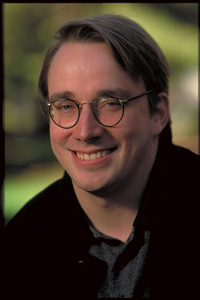
\includegraphics{images/linus.eps}}
%\caption{Linus Benedict Torvalds}
%\end{wrapfigure}
�к���Ժѵԡ���Թء����������ҧ㹻� �.�.  1991
�¹ѡ�֡������Է����ª�ǿԹ�Ź������� 
 Linus Torvalds \cite{JustForFun}.  Linus\index{general}{linus benedict torvalds@Linus Benedict Torvalds!Linux Torvalds}
�繤����ʹ���Ф�ء��աѺ�����������ҵ������. ��������繹ѡ�֡�һ�˹�觷������Է�����
Helsinki, �������ѡ�Ѻ�к���Ժѵԡ���ٹԡ����ᵡ��ҧ�ҡ�к���Ժѵԡ�÷����Ѻ������������ǹ�ؤ��. 
��÷���������ѡ�Ѻ�ٹԡ�����ͧ�繨ش������鹷������ʹ��֡�ҡ�÷ӧҹ�ͧ�к���Ժѵԡ��.

˹ѧ��� \emph{Operating Systems: Design and
Implementation} ��˹ѧ��ͷ������ҹ��Сͺ������¹����ǡѺ����ͧ�к���Ժѵԡ��. ˹ѧ������������¹�� Andrew Tanenbaum\index{general}{andrew tanenbaum@Andrew Tanenbaum} ������Ҩ��������Է�����㹻����������Ź��.  Andrew Tanenbaum
�͡�ҡ����¹˹ѧ�������ǡѺ�к���Ժѵԡ���������ѧ���ҧ�к���Ժѵԡ�â�Ҵ��硤�����ٹԡ�����ժ������ {\em �Թԡ�� (Minix)\index{general}{minix@Minix}} ����Ѻ������¹����͹�к���Ժѵԡ���ա����. 
˹ѧ�������������ç�ѹ��������繪�ǹ�����Դ��� Linus
���ҧ�к���Ժѵԡ�ô��µ���ͧ.  

㹻� 1991, Linux ���ͤ�����������ǹ�ؤ������ҹ. �������������ҫ����繤�����������ǹ�ؤ�ŷ����˹��»����żŢͧ Intel ��� 80386 ����к���Ժѵԡ�÷���Ҿ�����Ѻ����ͧ���������������� MS DOS. �͡�ҡ�������觫����к���Ժѵԡ���Թԡ���ҧ�ҡ�����ҵԴ���% 
%\glossindex{install}{��ù���������� OS ��è��˹��¤����Ӷ�����
%harddisk ������ҹ.} 
㹤�������������ͧ����ͧ��᷹ MS DOS ����Ѻ�֡�ҡ�÷ӧҹ�ͧ�к���Ժѵԡ��. ��������Թԡ�����к���Ժѵ����͡���֡����������͡����ҹ, �к��ҧ���ҧ��Թԡ����ҹ�����չѡ�����觷�������ͺ���{\em �����Թ������������ (terminal emulator) }�ͧ�Թԡ��. �Ҩ֧�Ѵ�Թ���������ҧ����������Թ������������%
\myvocab{t}{terminal emulator}{\emph{�����Թ������������}. ����������㹡���ʴ�����ٻ�ͧ����ѡ�ü�ҹ�ҧ˹�Ҩ��¡�û�͹��������Ҽ�ҹ�ҧ�������}%
����{\em ������������ (assembly language)} �ͧ.

���ͷ�����ҹ������ػ�ͧ����Է����¼�ҹ{\em ����� (Modem)} �ҡ����ҹ, �ҵ�ͧ���ҧ�����Թ��������������ӧҹ 2 ���ҧ������ѹ��� ��ҹ�����Ũҡ����������ʴ��ŷҧ˹�Ҩ�,
����Ѻ�����Ũҡ������������觵����������.
��÷ӧҹ�ͧ���ҧ��������ǡѹ����ѡ��÷�����¡��� {\em task switching}\index{general}{task switching} ����繾�鹰ҹ�ͧ�к���Ժѵԡ��.
����������Թ�������������������ҧ�纺ѹ�֡�������{\em ���ͻ���ԡ�� (floppy disk)}
���Щй�����ҷ���Ҩ����������ͧ{\em �ٵ (boot)} ������ҡ�蹿��ͻ���ԡ���µç. �ѭ�ҷ���ͧ�����ҡ���������ҵ�ͧ��ô�ǹ���Ŵ����ҹ�ҧ������纺ѹ�֡ŧ���촴ԡ��. �ѭ�ҹ�������ҵ�ͧ�֡������ǡѺ {\em file system} ���������Ͷ��. Linus
��¹{\em �������� (driver)} �ͧ���촴ԡ����з���������Թ�������������红�����ŧ���촴ԡ�쨹��. 㹷���ش�����Թ�������������������������, �����¹���������ҹ������ػ�����������¹���к���Ժѵԡ�÷�������й���. 

�к���Ժѵԡ����������ٻ����ҧ�Ѵਹ����� Linus �ӡ��{\em ���� (port)}\index{general}{port (�����)} %
\myvocab{p}{port}{\emph{����}(�����). ��ôѴ�ŧ�鹩�Ѻ�����, ����������麹�к���Ժѵԡ�÷��ᵡ��ҧ�ѹ����ʶһѵ¡���������������ᵡ��ҧ�ѹ��}\myvocab{x}{X window system}{\emph{X �Թ���}. �к�����ʴ��š�ҿ�ԡ���ҹ�ҧ���Ҿ��ٻẺ�ͧ˹�ҵ�ҧ���ºҹ. ���ç��âͧ MIT ���Ѳ�ҵ���Ҩҡ W windows system �ͧ Stanford. �к� X �Թ���������Թء�����ç��âͧ Xfree86 ��觾Ѳ�� X �Կ�����������Ѻ�մ��͡��촵�ҧ�. �ѧࡵ������¹��� X window ����� X windows.}
{\em ���� (shell)} 
����繵��������Ѻ����觨ҡ��������觵������к���Ժѵԡ��. �к���Ժѵ����������ó�������Ҿ���{\em �������������  C (C compiler)} �����.
������¤������������ö�����ʵ鹩�Ѻ�ͧ���������Ҥ������������Ѻ�к���Ժѵԡ�÷�������ҧ���. ������ͧ���, ����������, ��С����������ͧ��� Linus ����ͧ��������Դ�к���Ժѵԡ�÷�����¡��� ``�Թء��'' ��ѹ���.

��ѧ�ҡ���  Linus �Դ���к���Ժѵԡ�÷�������ҧ��ҹ�ҧ�Թ������. �ѡ�Ѳ�ҫͿ������ҡ�����š���ʹ�����������������ҧ�������ٹԡ���������Ѻ�Թء���� {\em �к� X �Թ��� (X window system)}%
, �ٷ��Ե���������ҧ���ҡ  Free Software Foundation (GNU)
�������. �͡�ҡ��þ���������������������, ������ҧ���ҧ���ҧ�������Ѻ�麹
�Թء��Ѩ�غѹ���������к���Ժѵԡ���ٹԡ������� {\em GNOME} �繵�. ��觷���Ӥѭ�ա���ҧ��͡�þ��쵵���к���Ժѵԡ���Թء���ͧ�������Ѻ{\em ʶһѵ¡������������� (computer architecture)} ���� ��  Atari, Alpha, SPARC �繵�.



% �Է�Ժѵ� (patent), �Ԣ�Է��� (copyright), �͹حҵ (license)
%\section{�͹حҵ����Է���㹡����Ϳ������}
\section{�����¡Ѻ�Ϳ������}
\mymemo{���ͧ�ҡ�����¹�����������Ǫҭ��ҹ������, �����ҷ������ǡѺ�Ԣ�Է���, �͹حҵ ����Է�Ժѵ÷���йӹ���Ҩ�����������ŷ�����§�ç. ����Ѻ�����ʹ㨡�س���˹ѧ����������䫴� \cite{thaiip} �������ǡѺ��������ҹ��Сͺ.}˹ѧ������������˹ѧ�������ǡѺ�Թء�������˹ѧ��ͷ������ǡѺ������. ����ա����§�������е�ͧ����Ƕ֧���ЫͿ�����������Ҩ����Թء�������������������ҧ�������������֧�����Ҩ� ``���'' ����������¤��������Ҩз����á���Ѻ�Ϳ����������ҹ��.

\subsection{�Ԣ�Է���}
{\em �Ԣ�Է��� (copyright)} \index{general}{�Ԣ�Է���}\index{general}{copyright|see{�Ԣ�Է���}} ����Է����������ҧ��ä�֧����ҡ�ŧҹ������ҧ. �ŧҹ㹷�������� �Ϳ������, ˹ѧ���, �Ҿ¹��, �ŧ �繵�. ������Է������Է���㹼ŧҹ�ͧ����ͧ�� �Է���㹡�â��, �Է�������������, �Է���㹡��ᨡ���� ���. �Ϳ�������Ԣ�Է����ͫͿ�����������Ѻ��ä�����ͧ�¡������Ԣ�Է���. ��÷������蹷���������Ңͧ�ŧҹ��������ͧ���Ѻ͹حҵ�ҡ������Է����͹������ŧҹ���. �Ϳ��������������Ԣ�Է�������Ϳ������������ա�ä�����ͧ��ҧ������ �蹫Ϳ���������С����{\em �Ҹ�ó����ѵ� (public domain)}\index{general}{�Ҹ�ó����ѵ�}\index{general}{public domain|see{�Ҹ�ó����ѵ�}}.

������ҧ�Ϳ���������Թء���������繫Ϳ�����������Ԣ�Է�����м�����ͤ�ͧ�Ԣ�Է��������� Linus Torvalds ����繼�����ҧ. �����ѡ���������Ҩ����á�������ͧ������Թء���ͧ���Ѻ͹حҵ�ҡ��� Linus ��͹�֧������. ��㹤����繨�ԧ���������ö���Թء����������ͧ��͹حҵ���й�� Linus �����͹حҵ��������{\em �͹حҵ (license)} ������¡��� GNU General Public License ����Թء�������ŷ�������ҧ���.

\subsection{�͹حҵ}
����������������ͧ��Ǣͧ����������, �Ϳ���������Թ��������Թ��ҷ���ҧ�ҡ�Թ��ҷ���仵ç���Ϳ���������Թ����ԧ��������ҡ�����ٻ����. ��������ҵԢͧ�Ϳ������, �Ϳ�������繢����ŷ������������͡�ҧ��ҧ���. ����ö�������觵����餹�����. ����Ѻ���������������Ш���ҵ�ͧ������ͧ��. �����ҵԢͧ�Ϳ���������ͧ�繻ѭ������Ѻ����Ե�Ϳ�������ԧ�ҳԪ��. ����Ǥ�Ͷ�Ҽ���Ե�Ϳ�����������ѭ�ҡѺ�������Ϳ������, �������Ϳ������������ö������ᨡ����, ������Ѻ������������������͡. �繼�������Ե�Ϳ�������������ö���Թ��áԨ���¡�â�«Ϳ��������. ����ͧ�繷���Ңͧ{\em �͹حҵ (license)}.\index{general}{license|see{�͹حҵ}}\index{general}{�͹حҵ}

�»á�����ǫͿ����������͹حҵ㹡����ҹ�ӡѺ�Ҵ���. �͹حҵ�����͵�ŧ�����ҧ������ҧ, ��Ңͧ, ���ͼ���˹��«Ϳ������Ѻ��������Ѻ�Ϳ����������������Ңͧ��͵�ŧ��ᵡ��ҧ�ѹ�͡仵���ó�. �»á��, �͹حҵ�ШӡѴ�Է����ҧ���֧��з���Ѻ�Ϳ������������������ᨡ, �����Դ��駫Ϳ������ŧ�����ͧ�����������Թ˹������ͧ�繵�. ��͹���㹷ҧ��Ժѵ�, �������Ϳ��������������ö��з��������ҹ��������繡������Դ��͵�ŧ��ж������դ����Դ, �Ҩ�١���Թ��յ�������µ���.


\subsubsection{GNU General Public License}\index{general}{gnu general public license@GNU General Public License}

�Թء�����������������������ͺ��������ͧ��÷����� (copying), ���ᨡ���� (distribution) ��С����� (modification). �͹حҵ����Թء�����͡������ {\em GNU General Public License (GNU GPL)}. �͹حҵẺ GPL\index{general}{gpl@GPL|see{GNU General Publice License}} ������ҧ�����ͧ��÷�����¡��� {\em Free Software Foundation}\index{general}{free software foundation@Free Software Foundation}\index{general}{gnu@GNU} 
%%%
%\marginpar{\includegraphics{gnu-head-sm.eps}}
\mymemo{Free Software Foundation ��ͧ�������������ѧ�š��ë�觡�͵���� Richard Stallman
����ͻ�{�.�.} 1982. �ش���ʧ��ͧͧ��ù�������ҧ�к��ٹԡ��������. �Ϳ���������ժ������§���Ѳ����ͧ��ù������ GNU C compiler,
GNU Emacs ���. 

Free Software Foundation �ժ������¡�������� GNU �繤����Ẻ recursive �ͧ����� ``{\bf G}NU is {\bf N}ot {\bf U}nix''}
%%%
��͵����д��Թ����¹�� Richard Stallman\index{general}{richard stallman@Richard Stallman}. 

�͹حҵẺ GPL ����ͧ��������Թء���ҧ�ҡ�к���Ժѵԡ�÷�����. �»á�������к���Ժѵԡ�èоѲ����ͧ������ͺ���ѷ㹡��������. ����ա���Դ�����ʵ鹩�Ѻ���Ҹ�ó�, ������������ö����������ᨡ������餹��蹵����. �к���Ժѵԡ���Թء���դ����Դ���ᵡ��ҧ�Ѻ��觷�����������ҧ����ԧ. �Թء�����к���Ժѵԡ�÷����. ������ͧ������Թء������դ������繷���ͧ�����Թ����, ����ö{\em ��ǹ���Ŵ (download)}
�ҡ�Թ������ \cite{kernel}. ��м�������Է������ᨡ���µ����������Դ�����µ�Һ��������ѧ��ԺѵԵ���͹حҵ GPL �к����. ����� ``���'' 㹷������������¤�������Ҥ��� ``�ٹ��'' �����¶֧������ ``���������'' ��������з���. ��÷���Թء�����͹حҵẺ GPL �ռŴդ��������������������. �Դ�͡�����ѡ�Ѳ�ҫͿ����������ö�֡�����ʵ鹩�Ѻ, ��оѲ�һ�Ѻ��ا������������������觢��. GPL �ѧ�кض֧{\em �ҹ�׺�ʹ (derived work)} �ͧ�Ϳ�����������͹حҵ��Ẻ GPL ������ҧҹ�׺�ʹ�����͹حҵẺ GPL �»�����. ����Ǥ�Ͷ���繧ҹ����׺�ʹ�Ҩҡ�ҹ GPL �ҹ��鹵�ͧ�� GPL ����. �ؤ����������з�����, ᨡ����, ������ʵ鹩�Ѻ�ͧ�ҹ�׺�ʹ��. �������ö�����������˵ط���Թء����ѹ���ҧ�����������ա����䢻�Ѻ��ا���ѹ���·ѹ�˵ء�ó��繼Ţͧ��÷���Թء�����͹حҵ GPL ����ͧ.

\subsubsection{GNU Lesser General Public License}\mymemo{�������͹حҵ GNU Library General Public License.}
����Ѻ�ҹ�׺�ʹ���ӵ�����������ʵ鹩�Ѻ�ͧ�Ϳ�����������͹حҵẺ GPL, ����͹حҵ�к������ҧҹ�׺�ʹ�е�ͧ���͹حҵẺ GPL ��»����� \cite{gpl}. ���¤������������ԧ�ҳԪ�����׺�ʹ���������ʵ鹩�Ѻ�ҡ�Ϳ�����������͹حҵẺ GPL ��ͧ���͹حҵ��Ẻ GPL 仴���. 㹡ó��Ҩ�繼�������ԧ�ҳԪ�����ЫͿ���������Ե�͡�ҨС����繫Ϳ������������ö������, ᨡ������, �����ʵ鹩�Ѻ����»�����. �˵ع���ͧ�ҧ FSF �֧�͡�͹حҵ������¡��� {\em GNU Lesser General Public License (LGPL)} ���Ŵ����Է���ͧ�������硹��µç����Դ�͡�����Ϳ�������ԧ�ҳԪ������ö�����ʵ鹩�Ѻ�ͧ�Ϳ�����������件֧{\em �ź���� (library)} ������͹حҵẺ GPL ���·��ҹ�׺�ʹ����ѧ�����͹حҵ�ͧ����ͧ�������� GPL ����.

��ػ����� LGPL �������е�ͼ�������ŧ (lesser) �������º�Ѻ�͹حҵẺ GPL. 㹷ҧ�ç�ѹ�����繡���Դ�͡�����Ϳ�������ԧ�ҳԪ�������繧ҹ�׺�ʹ��Ϳ�����������ź���շ�����͹حҵ�� GPL �����ѧ���͹حҵ�ͧ����ͧ. 

��õդ����ҹ�׺�ʹ��Ҥ�������ѧ�����¡�Ш�ҧ�ҡ�ѡ, ����ͧ¡������ͧ�ͧ������. ������ҧ�ҹ�׺�ʹ���Ѵਹ���������, �������, ��Ѻ�觧ҹ�����Ẻ GPL �������繧ҹ�׺�ʹ���ҧ�����Ѵ. �Ϳ�����������ź���շ����������ҧ�ͧ��������繧ҹ�׺�ʹ�蹡ѹ. �ѧ����ź���շ�����ҵðҹ�����ѹ�ҡ�ͧ FSF �ѹ�����͹حҵẺ LGPL ���ź���� C �ͧ GNU �繵�.\mymemo{��ä����������������������¹�������� C �����ź���� C �»�����. �����ͧ�ҡ�ź���� C �ͧ GNU ���͹حҵ�� LGPL ���Щй�������������ź���չ�������繵�ͧ�� GPL ����.}



%\mymarginpar{\scalebox{0.6}{\includegraphics{images/gnu-head-sm.eps}} }. 
%%% myvocab
%\myvocab{Free software : �Ϳ����������\par Run : ��зӡ��, �ѹ\par Copy : ������, ��ͻ���\par Distribute : ᨡ����}
\subsubsection{�͹حҵẺ����}

㹢�з���Թء�����������͹حҵẺ GPL, �������ҧ���������������к���ҹ�����繵�ͧ���͹حҵẺ GPL ����. ����������Ѻ�Թء�������Ҩ�����͹حҵẺ���� \cite{license} ���������ҧ����ʴ�㹵��ҧ��� \ref{tab:license}.

\begin{table}
\center
\caption{������ҧ�������ͧ�͹حҵ��ҧ��觵����������}
\medskip
\label{tab:license}
\begin{tabular}{p{.4\linewidth}p{.5\linewidth}}
\hline
\multicolumn{1}{c}{�������ͧ�͹حҵ} &  \multicolumn{1}{c}{������ҧ}\\
\hline
GPL-Compatible Free Software Licenses & GPL, LGPL, Public Domain, X11 License, BSD (modified)\\
GPL-Incompatible, Free Software Licenses & BSD (original), Open Software License, Apache License, Mozilla Public License (MPL), Q Public License (QPL), PHP License\\
Non-Free Software Licenses & Open Public License, Aladdin Free Public License, Microsoft's Shared Source License\\
\hline
\end{tabular}
\end{table}

\subsection{�Է�Ժѵ�}
{\em �Է�Ժѵ� (patent)}\index{general}{�Է�Ժѵ�}\index{general}{patent|see{�Է�Ժѵ�}} ���˹ѧ����Ӥѭ����͡������ͤ�����ͧ��û�д�ɰ� ���͡���͡Ẻ��Ե�ѳ��. ��û�д�ɰ�������֧�����Ըի�������鹵͹�Ը� (algorithm) ����. ���¤�����Ҷ������仨��Է�Ժѵâ�鹵͹�Ը����͹���Ǽ��Ѳ�ҫͿ���������鹵͹���ǡѹ㹡�����ҧ�Ϳ�����������ҨФԴ�ͧ��������ͧ��͹حҵ���ͨ��¤�ҵͺ᷹�Ѻ����訴�Է�Ժѵù�鹡�͹. 

�ѭ�Ңͧ�Է�ԺѵáѺ��þѲ�ҫͿ���������������¡ó�. �������Һ���ѷ�ҧ��觨��Է�Ժѵ������йѡ�Ѳ�ҫͿ�������������ҧ�Ϳ�������ѹ˹�觫��仵ç�ѹ�����Ңͧ�Է�Ժѵù��. ����ѷ�������Ңͧ�Է�Ժѵ��Ҩ�������ҫͿ��������ѡ�Ѳ�ҫͿ�����������ҧ���Ըա�����ǡѺ������ѷ���Է�Ժѵ���� �����ѷ����ͧ��ͧ�ѹ��. ����ѷ�Ҩ��������ͧ��º��ж�ҫͿ��������Ҵ�ԧ�������Է�Ժѵâͧ����ͧ�Դ���Ѻ���������դ����ҡ, ����ѷ�����������ͧ��ͧ�������¡�纤�ҵͺ᷹�ҡ��������ͼ�����ҧ�Ϳ������������. �Ըչ���ͧ���Ըշ���������ҧ˹�觫������繸�������ùѡ����ѧ�դ�����੾������Ѱ����ԡ������ӹѡ�ҹ���Է�Ժѵ��������ҡ��è��Է�Ժѵ�. ����դ����Է�Ժѵ��ҡ����á���������ҡ��ҹ��. 

�ѭ������ǡѺ�Է�Ժѵ��ա���ҧ�����è��Է�Ժѵá����Ը�㹡�á�з����ҧ����ҧ˹�觷������Դ��. ������ҧ�� Amazon.com ��ҹ���˹ѧ��ͺ��Թ����������˭��騴�Է�Ժѵ�����ǡѺ��鹵͹��ë��ͧ͢���Թ�������¡�����˹�觷� (one-click purchasing) \cite{amazonpatent} ��觢�鹵͹�������觷�����㹡�ë��͢�¢ͧ����Թ�������������Դ��. 



\section{�Ϳ����������}
��ͧ�Ӥ��������ա��硹������ GPL ����͹حҵ�����Ϳ������. \emph{free software} \cite{fsf,freesoftware} ����������������{\em �Ϳ����������}%
\mymemo{���������·�����ͤ������¤���� free sotfware ��������{\em �Ϳ����������}. �������Ѻ�Ѿ����ҿ�իͿ�����������Դ�����Ѻʹ�����. ����㹷�����ѧ���¶֧���շ���բͺࢵ. ��������շ����ҡ�з����á����.}%
\index{general}{�Ϳ����������}, ���㹷����������������������ǡѺ�Ҥ�. ����Ǥ�ͼ����������з��С�зӡ�� (run), ������ (copy), ᨡ���� (distribute), �֡��, ��Ѻ��ا����¹�ŧ�Ϳ������. �觤�����������������дѺ���:
\begin{itemize}
\item ������дѺ��� 0: ����з����������ö��Ϳ������������㹡ó������͡����
\item ������дѺ��� 1: �����㹡���֡�ҡ�÷ӧҹ�ͧ�Ϳ������, ����¹�ŧ��䢫Ϳ������������ͧ���. ���¤���������ʵ鹩�Ѻ�Դ�µ�ͼ�����ͧ���.
\item ������дѺ��� 2: �����㹡��ᨡ���«Ϳ���������������.
\item ������дѺ��� 3: �����㹡�û�Ѻ��ا�Ϳ���������բ��, ᨡ��������Ҹ�óЪ�������������Ѻ����ª��ͧ��û�Ѻ��ا�����ѹ. ��÷��к���بش���ʧ����, ���ʵ鹩�Ѻ��ͧ�Դ�´���.
\end{itemize} 
�Ϳ������������¡������繫Ϳ���������� (free software) ��ͧ��ͧ���Сͺ��ҧ�鹷������ú. �ա��С��˹�觤�� free software ��������¤������������Ҥ�. �Ҩ���ա�â�����Թ��ҡ�������繫Ϳ���������� (free software) �����դس���ѵԷ�����������������.



\section{��ྐྵ�����}

�֧���������ա�á�˹��������¢ͧ����� free software ����ǡ���, ����� ``���'' ������ѧ����ѡ�����˵����ؤ�ŷ�����Ѻʹ�����. ������ҧ��������ҧ���ҧᨡ����������������ö�������֡�����ʵ鹩�Ѻ��. �ҧ��������¡�ѹ��� ``���'' ������{\em �Ҹ�ó����ѵ� (pulic domain)}. Public domain ���¶֧��������{\em �Ԣ�Է��� (copyright)}\index{general}{�Ԣ�Է���}\index{general}{copyright|see{�Ԣ�Է���}} ������ͧ, ���������ö�����á����觺ҧ�ó������Ŵ������. �ҧ����� ``���'' ����੾�кؤ�źҧ��������͡������������þҳԪ��. �����Ѻʹ��ҧ�����ҹ�������Դ���������{\em ��ྐྵ����� (open source)}\index{general}{��ྐྵ�����} ᷹����� free software. 

�Ϳ������������¡���������ྐྵ����ʹ�鹵�ͧ��Сͺ���¢�͡�˹��������ҧ����˹��� Open Source Initiative \cite{osi}.%
%\marginpar{
\includegraphics[scale=0.8]{osi.eps}}
\mymemo{Open Source Initiative (OSI) ��ͧ��ó��������ѧ�š����ըش���ʧ������������ʹѺʹع�Ϳ������Ẻ��ྐྵ�����. �ա���͡��Ѻ�ͧ�Ϳ��������ྐྵ�����, ����ҧ��� �繵�.} ������ҧ�蹫Ϳ��������ྐྵ����ʵ�ͧᨡ����������, ���մ�ѹ�ؤ��㴺ؤ��˹�������Ҩ������ͪҵ���������. ����ö������㹧ҹ㴡��������մ�ѹ. �Դ�����ʵ鹩�Ѻ�繵�. �����ҹ����ö��ҹ�ӨѴ�Ѵ�����ͧ��ྐྵ������������´���������ҡ���䫴�ͧ Open Source Initiative.


\section{�����ҵ���Фس�ѡɳТͧ�Թء��}

\begin{description}
\item[�Դ�������������������]\mbox{}\\
���ͧ�ҡ�Թء�����͹حҵẺ GPL �����֧���Է�����з�����, �֡�����ʵ鹩�Ѻ, ������ʵ鹩�Ѻ�������ͧ��õ�Һ��ҷ�����ʵ鹩�Ѻ�������¹�ŧ�Դ�µ���Ҹ�ó�. �Թء������ö������Ŵ��ҡ�Թ������, ���͡�ͺ���ᨡ���«��͢������ٻẺ�ͧ���͵�ҧ��� CDROM �繵�. 㹡óշ������дǡ������Ŵ�ҡ�Թ������, ���������ö���͡���� CDROM ��ʷ�Ժ�Ǫѹ������������Ǩҡ����Ե��ʷ�Ժ�Ǫѹ�µç.


\item[��觵��ͧ��͹�ͤ�����������ͨҡ������]\mbox{}\\
�����ѭ�����͢��ʧ��·���Դ�ҡ�Թء���¾�鹰ҹ���Ǽ�����ͧ��觵��ͧ����ѡ. ���ͧ�ҡ�Թء�����ҧ�ҡ����������Թ������������Թ��ҷ�����ҧ�Ѳ���º���ѷ㴺���ѷ˹��, �֧�繡���ҡ�����Ѻ��Сѹ����ʹѺʹع�����ҹ (support) �����ҧ������. ������èе��˹ѡ����������ҵ�ͧ��觵��ͧ��͹�����ͻѭ�����͢��ʧ���㹡����ҹ. ������Ҩ�е�ͧ�Ң����Ũҡ˹ѧ��������Թ������, �����͡����ҹ�ͧ. ����������ö��ѭ���������Ҥӵͺ����͡��Ҩ�ж�����������ͼ����ҹ����蹷ҧ mailing list, webboard, newsgroup ��� ��Сͺ�Ѻ�����ŷ�赹�ͧ�����. 

\item[����Է���Ҿ]\mbox{}\\
�Թء�����к���Ժѵԡ�÷��{\em �ʶ��� (stable)} ����� {\em ������� (downtime)} ���. ���ʵ鹩�Ѻ�ͧ�к���Ժѵԡ�����Ѻ��õ�Ǩ�ͺ��з��ͧ���ҧ�ա�͹����{\em ����� (release)} ������������. ��͹�����������÷������ó�Ẻ, �����������������ҹ�ҧ���ҧ�Ҩ���ժ�ͧ������ѧ�ҡ�͡��С����. �·���仪�ͧ�������͢�ͼԴ��Ҵ����ҹ��ж١��§ҹ��ͼ��Ѳ�����������蹶Ѵ�. ����繪�ͧ����������ǡѺ������ʹ��¢ͧ�к����ҧ�����ç���Ҩ�����Ѻ���������ҧ�Ǵ����������ó�.

\item[��ҹ�������дѺ]\mbox{}\\
�Թء������ö��ҹ��Ѻ���������������дѺ�����ҹഡʷ�ͻ����� GUI, ���֧�дѺ�Կ��������鹤����ʶ�����Ф����дǡ㹡�û�Ѻ�觷ҧ {\em CUI (Command Line User Interface)}.
�Թء�������§������Ѻ������������ǹ�ؤ����ҹ��, �Թء���ѧ����ö���{\em �к������� (embedded system)} ���˹��¤������բ�Ҵ�����ШӡѴ. 

\item[�����ҹ�����Ѻ�к���Ժѵԡ������]\mbox{}\\
�Թء������ö��ҹ�����ŷ��ѹ�֡㹴ԡ�����к���Ժѵԡ����  MS-DOS, Microsoft Windows, SVR4, OS/2, Mac, Solaris ��. �ҧ��ҹ�������, �Թء��ʹѺʹع{\em �������������� (network layer) }���»������� {\em �������� (Ethernet)},  FDDI, Token ring ���. ����ö�ѹ{\em �����亹��� (Binary Program)} �ͧ DOS ����  MicroSoft Windows ���¼�ҹ������������  VMWare.

\item[�ִ�ҵðҹ]\mbox{}\\
�Թء�����к���Ժѵԡ�÷���������ҧ�¤����º��Թ������, ���Щй���ҵðҹ��ҧ�����觨�����������þѲ���к����Թ�������ǡѹ. �ҵðҹ�ѧ������繷���Դ���������Ѻ�ѹ�������  POSIX, {\em ���������ⵤ�� (network protocol)}%
\myvocab{p}{protocol}{\emph{��ⵤ��}. ��͢�͵�ŧ, �Ըա��㹡�á�зӡ�����ҧ����ҧ˹��. �� HTTP protol �繢�͵�ŧ, �Ը�} ��ҧ��繵�.
\end{description}


\section{��ʷ�Ժ�Ǫѹ}\index{general}{distribution@Distribution|see{��ʷ�Ժ�Ǫѹ}}

�ҡ�����������Ǣ�ҧ������Թء��㹤������·�������¶֧��ù�����������������ҧ�������ѹ���к�. ��ù�����������������ҧ�������ѹ����ᨡ���� (distribute) ���ͤ����дǡ�ͧ����������¡���{\em ��ʷ�Ժ�Ǫѹ (distribution)}. ��ʷ�Ժ�Ǫѹ�ҧ���¡����ԧ�ҳԪ��, �ҧ���¡����ҧ��������Ѥ��������ѧ�Ż���ª��. �֧���ҧ���¨��繴�ʷ�Ժ�Ǫѹ�ԧ�ҳԪ�����, ����ǹ�˭����Ǽ��������ö������Ŵ����������¤�����������ʷ�Ժ�Ǫѹ����ҹ��. 

��ʷ�Ժ�Ǫ�����Ф����դ���ᵡ��ҧ�ѹ���������´ ���ٻ��ҧ˹�ҵ�ഡʷ�ͻ, �����ҡ���¢ͧ{\em ������Դ��� (installer)}, {\em �к��Ѵ�����ࡨ (package management)}, ��������Ϳ�������ԧ�ҳԪ�����繵�. ����觷��ء��������͹�ѹ������㨢ͧ��ʷ�Ժ�Ǫѹ���Թء�����������к���ԺѵԾ�鹰ҹ, �Ǻ����Ϳ���������յ�ҧ�������к���ҹ. 

��ѧ�ҡ����� Linus ��С���к���Ժѵԡ�÷�������ҧ��鹼�ҹ�ҧ������ػ����, ���ǻ� �.�.1993 Soft Landing Software (SLS) �¹�� Peter McDonald ����������ҧ��ʷ�Ժ�Ǫѹ������á�.\mymemo{�ҡ����ѵ���ʵ��������¹�鹤������������ö�к�����Ѵ��Ҵ�ʷ�Ժ�Ǫѹ�����á�����������������繼�����ҧ} ��ʷ�Ժ�Ǫѹ���㹪�ǧ������������� Yggdrasil ��觷�� SLS ��� Yggdrasil ����繷�����㹻Ѩ�غѹ. ��ʷ�Ժ�Ǫѹ������¡��һ��ʺ�������������繷�����ѡ�ѹ���ҧ�������㹻Ѩ�غѹ���� Slackware, Red Hat, Debian �繵�.


\subsection{{\latintext Slackware}}\index{general}{slackware@Slackware}%\marginpar{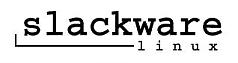
\includegraphics[scale=0.35]{slackware_logo.eps}}

SLS �繴�ʷ�Ժ�Ǫѹ�����á�����ѧ������ͧ�ҡ����Ѻ��������价��Դ����������������Թء��. ��� Patrick Volkerding\index{general}{patrick volkerding@Patrick Volkerding} �繼������ش��͹����ҹ��������ҧ��ʷ�Ժ�Ǫѹ����ժ������ {\em Slackware}\index{general}{slackware@Slackware} �����������͹�Զع�¹ �.�.1993. ����ҵ���Ҵ�ʷ�Ժ�Ǫѹ��������繵�Ẻ��ʷ�Ժ�Ǫ�蹢ͧ������������. Slackware �鹤������º���¢ͧ�к���Фӹ֧�֧�����ҹ. �������ҧ����������㹴�ʷ�Ժ�Ǫ�蹹�������ҧ������������� \cmd{tar} ��� \cmd{gzip}.


\subsection{{\latintext Red Hat}}\index{general}{redhat@Red Hat}%\marginpar{\includegraphics[scale=0.65]{redhat_logo.eps}}

���ǻ� �.�.1994 \cite{redhathist}, Red Hat �繴�ʷ�Ժ�Ǫѹ�ԧ�ҳԪ���á���������Դ������������� {\em Graphical User Interface (GUI)}. �����˵ع���ͧ������� Red Hat �繷������ѹ���ҧ�������. Red Hat �ըش�蹷��{\em ��èѴ�����ࡨ (Package Management)}, ������Դ������{\em ��������¤Ǻ����к� (System Management Utilities)}. 

Red Hat ��������Ѵ�����ࡨ������¡��� {\em RPM (Red Hat Package Management)}\index{general}{rpm@RPM|see{Red Hat Package Management}}.\index{general}{redhat package management@Red Hat Package Management} ���������ö�Դ���������������ٻ�ͧ��� \cmd{.rpm}. ����� {\latintext\cmd{rpm}} �ШѴ��õԴ���{\em 亹������ (binary file)}, ���������Ǣ�ͧ�Ѻ��������, �����͡����ҹ����������� {\latintext\cmd{.rpm}} �������á��������������. ��ѡ�ҡ���Դ�������ҧ����� {\latintext\cmd{rpm}} ��{\em ��Ѻ�� (configure)} ����������������ҡѺ�к�������������кѹ�֡�����ŷ������ǡѺ����������{\em �ҹ�����š�èѴ�����ࡨ (Package Management Database)}. ���������ö{\em �ѹ�Թʵ���� (uninstall)} ������������ͧ����͡�ҡ�к������ҧ���´�´�������� {\latintext\cmd{rpm}} �蹡ѹ. �к��Ѵ�����ࡨ��ź������������ҧ�������Ǣ�ͧ������ѵ��ѵ�.
������Դ��駷������ GUI ����дǡ��ͼ��������������͵Դ����Թء��. ��ѧ�ҡ���Դ����Թء������, ���������ö��Ѻ���к���������ͧ�����������ٷ��Ե���������ҧ�.

Red Hat �繴�ʷ�Ժ���ԧ�ҳԪ����㹢�����ǡѹ͹حҵ�������������á��������Ŵ������ʵ鹩�Ѻ, ������Դ���, �����ࡨ亹��յ�ҧ� ����պ�ԡ�������ࡨ����բ�ͺ����ͧᨡ���´���. ����Ǥ�ͼ�����ͧ�� Red Hat �����繵�ͧ�����蹫մըҡ Red Hat ������ö�� Red Hat ��, ��� Red Hat ����������ժ�ͧ��������ǡѺ������ʹ��¡�����ö�ѻഷ��ࡨ����������¤�������. 

����ͻ��»� �.�. 2003 �ҧ Red Hat \cite{eol} ���С�ȡ��������� (end of life) �ͧ Red Hat Linux 7.1, 7.2, 7.3 ��� 8.0. ��û�С��������������ǡѺ�����ش����ԡ���ѻഷ, ��ش�������ԡ��, ��ش������ҧ��ࡨ��䢢�ͺ����ͧ�ͧ Red Hat Linux ��蹷���ӡ��� 8.0 ������鹻� �.�. 2003. ��� Red Hat Linux 9 ��������آ��������͹����¹�� �.�. 2004. ��������ͧ�������к�ԡ���ѻഷ��ҧ�ͧ Red Hat ��ͧ�� Red Hat Enterprise Linux ��觨����ᨡ������ࡨ亹�������������Դ��駵�ҧ�ҧ�Թ������. Red Hat �ѹ���鹸�áԨ�ҧ��ҹ�������ԡ���ҡ���ҡ�â�µ����ࡨ. ������ͧ����� Red Hat Enterprise Linux ��ͧ����к���ԡ�âͧ Red Hat ��觨��������дѺ������ԡ����ࡨ���������ҡ�բ�ͺ����ͧ, �Դ����ͺ����ҧ���Ѿ��, ���ͺ�ԡ�ö֧��� ��� \cite{rhel}.

�͡�ҡ Red Hat Enterprise Linux ���� Red Hat �ѧ��᡹��ʹѺʹع�Ѳ�Ҵ�ʷ�Ժ�Ǫѹ����㹪��� Fedora \cite{fedora} ����Դ���ҧ�����ʹ㨪��¡ѹ�Ѳ���繴�ʷ�Ժ�Ǫѹ����᷹ Red Hat Linux �����������.


\subsection{{\latintext Debian GNU/Linux}}\index{general}{debian@Debian}%\marginpar{
\includegraphics[scale=0.35]{debian_logo1.eps}
\includegraphics[scale=0.35]{debian_logo2.eps}}

Debian �繴�ʷ�Ժ�Ǫѹ���Ѳ����������Ѥèҡ�����š�ժ����繷ҧ������ {\em Debian GNU/Linux}. Debian ��͡��Դ�¹�� Ian Murdock ������ѹ��� 16 �ԧ�Ҥ� �.�.1993. ��� Ian ��ͧ��÷��з�����ʷ�Ժ�Ǫѹ�����������Դ��������ش���ó���Ẻ�Թء����� GNU. ������ҧ��ʷ�Ժ�Ǫѹ������Ѻ�ع�ҡ Free Software Foundation ������˹�觻յ������͹��Ȩԡ�¹�� �.�.1994 �֧��͹��Ȩԡ�¹�նѴ� \cite{debianhistory}. ���ͧ͢ Debian (Deb-ian) �Ҩҡ���ͧ͢������ҷ���ժ������ Deborah ��Ъ��ͧ͢���ͧ Ian ����ѹ�繪��ʹ�ʷ�Ժ�Ǫѹ.
 
�ش�蹢ͧ Debian ����繴�ʷ�Ժ�Ǫѹ��������ѧ�š���, �Դ���������͡�ʡѺ�ѡ�Ѳ�ҷء�����ʹ������Ѳ�Ҵ�ʷ�Ժ�Ǫѹ. ��������ӹ�¤����дǡ�������ǡѺ��èѴ�����ࡨ������������ \underline{A}dvanced \underline{P}ackage Managemen\underline{t} �������¡������� APT.\mymemo{������Ѵ�����ࡨ��ѡ�ͧ�к��Ѵ�����ࡨ APT ���� \cmd{apt-get}, \cmd{apt-cache} ���.} ��觷�����ػ��ä����Ѻ��������������õԴ��駫��������Դ��駨�������Ẻ�硫��������㹢�еԴ��駨��ա�ö���Ӷ������ǡѺ��û�Ѻ���������ҧ������͡�Դ��駴���. ��Ҽ������������¡Ѻ�Թء���Ҩ��������㨷�����������ö�ͺ�Ӷ�����������. ���ҧ�á���������� Debian �ѡ�еԴ��駵���к���Ժѵԡ����§��������������к��Ѵ�����ࡨ APT �ѻ�ô�к���Ժѵԡ�����ѹ������������. ����������繵�ͧ�Դ����к���������������� Debian ��С���͡����������ش. 

����͵Դ��� Debian ���Ǽ��������ö���͡�������ͧ Debian ��������ҹ�����Ẻ����
\begin{description}
\item[Stable] \mbox{}\\
���к�����Ǻ�����ࡨ�Ϳ�������ҧ����ʶ�������ա���Ѻ�ͧ�繷ҧ��èҡ��� Debian �ҡ�ըش�����ͧ��ҹ������ʹ������͢�ͼԴ��Ҵ����, ���ա���͡��ࡨ�ѻഷ������. �����\emph{�ʶ��� (stable)} 㹷�������¶֧�Ϳ��������ࡨ��ҧ���������к����Ѻ��÷��ͺ, ��Ǩ�ͺ���ҧ����ǹ��͹�������ࡨ����������к�. �������ࡨ���������к� stable �բ�ͺ����ͧ����\emph{��� (bug)} %
\myvocab{b}{bug}{\emph{���}, \emph{��ͺ����ͧ}. ��ͺ����ͧ�ͧ�Ϳ��������ѧ�ҡ�����Ңͧ�Ϳ�������鹻�С���͡��ǫͿ��������}%
���·���ش. ����ա�þ���ͼԴ��Ҵ���ҧ�����ç�蹢�ͼԴ��Ҵ��ҹ������ʹ��¢ͧ��ǫͿ���������ա���͡��ࡨ�ѻ�ô������Ѻ�����������·���Ţ�����ѡ�ͧ�Ϳ�����������ѧ��������, �����������¹��ࡨ����������. 㹡óչ���բ�ʹշ����ҡ����ҹ�ͧ�Ϳ�������ҧ������Ҩ����Ըա�������͡�û�Ѻ���ѧ����͹��������繫Ϳ�������������������. �ѧ����к�Ẻ stable �֧���������Ѻ�����ҹẺ���������. 

㹷ҧ��Ѻ�ѹ, �Ϳ���������ʶ����դ��������繹����ҫͿ������������蹤�͹��ҧ���. �Ϳ�����������͡�����֧�����դس���ѵ�������������Ҩ���բ�ͺ����ͧ����ѧ����辺�����ҡ�֧����������ʶ���. �����˵ع���ͧ�������ࡨ��ҧ������������к� stable �֧��͹��ҧ����������º�Ѻ�к�Ẻ���.

\item[Testing] \mbox{}\\
���к���������ࡨ����ҹ��÷��ͺ���дѺ˹�觨ҡ unstable �����ࡨ��ҧ�����ҹ���բ�ͺ����ͧ���ͺ�꡹��¾ͷ����繵��᷹��ࡨ�������к� stable ����. �к�������������Ѻ������ͧ�����Ϳ������������������ʶ����дѺ˹��. �Ҩ�������к�ഡʷ�ͻ��ӡ�觡Ѻ������������դ������繵�ͧ��ëͿ��������������������ͧ�����ҡ����ش.
\item[Unstable] \mbox{}\\
���к��������ࡨ������������ش�������ա���Ѻ��Сѹ��Ҩ�����յ�����Ҵ��ѧ. �ҧ��ࡨ�Ҩ���ѧ�բ�ͺ����ͧ����ͧ���. �к�����ժ������ unstable ����Ť���������� ``����ʶ���'' �����������¤�������ʶ��è�ԧ������ҹ�����. �к�������������Ѻ������ͧ�����Ϳ�����������������ش��е�ͧ��÷��ͧ��������ö�����ͧ�Ϳ���������.
\end{description}

\subsubsection{�������ʡ�þѲ��}
�к�����Ẻ����{\emph{�������ʡ�þѲ�� (code name)}\gindex{code name}\gindex{�������ʡ�þѲ��} ��觹��Ҩҡ���͵���Ф���Ҿ¹������ٹ����ͧ Toy Story. �Ѩ�غѹ�к� stable �ժ������ʡ�þѲ����� Sarge, testing �ժ������ ???  ��� unstable �ժ������ Sid. �������ʡ�þѲ�Ңͧ unstable ���������¹�ŧ������¡��� Sid ����. ��ǹ�������ʡ�þѲ�Ңͧ�к����������¹��������������ա������͹����� Sarge �繪������ʡ�þѲ�Ңͧ testing �ҡ�͹. ������к��դ����ʶ����繷������Ѻ�֧����͹������� stable ���ѧ�ժ��������� Sarge ����͹���. ��ǹ testing ���ա�õ�駪����������.


\subsection{{\latintext Gentoo}}\index{general}{gentoo@Gentoo}%\marginpar{
\includegraphics{gentoo-tiny.eps}}

Gentoo �繴�ʷ�Ժ�Ǫѹ����͹��ҧ�����С�ȵ�Ǥ�����л���ҳ��͹�չҤ��� �.�.2002. ��ʷ�Ժ�Ǫѹ������͡�ѡɳ���ⴴ��ᵡ��ҧ�ҡ��ʷ�Ժ�Ǫѹ��蹷������ࡨ�ͧ�����ʵ鹩�Ѻ�ͧ�Ϳ���������ͧ��õԴ���, ���к���èѴ�����ࡨ������������դ����״�����٧㹡�û�Ѻ���к�. 

Gentoo ���к���äǺ�����ࡨ������¡��� \emph{portage}\mymemo{������Ѵ�����ࡨ��ѡ�ͧ�к��Ǻ�����ࡨ Portage ���� \cmd{emerge} ��� \cmd{ebuild}.} \index{general}{portage}������Ѻ�ǤԴ�Ҩҡ�к� port �ͧ�ٹԡ�� BSD. �к��Ǻ�����ࡨ�������ö����, ������Ŵ, ��䢤�����鹡Ѻ��ࡨ���� (package dependency) ��еԴ�����ࡨ����ͧ��������ѵ��ѵ������ǡѺ�к� APT �ͧ Debian. ��ࡨ�ͧ Gentoo ������������, ��������ʵ鹩�Ѻ�������ʤ�Ի��͡������ʵ鹩�Ѻ�������˹, �բ����Ţͧ�Ըդ�������еԴ���. ��õԴ�����ࡨ�բ�鹵͹��ҧ������ô�����Ŵ���ʵ鹩�Ѻ, ��õ�Ǩ�ͺ��������ѹ��Ѻ��ࡨ����, ��������еԴ���. 㹪�ǧ�ͧ��ä�����, �������������͡��Ѻ�觤�ҵ�ҧ����Ҩ���ռŵ�ͻ���Է���Ҿ��÷ӧҹ�蹵�����͡�������������СѺ˹��»����żŢ����ŷ����, ���ͻ�Ѻ������͡�͹���ҧ�ͧ��ࡨ���������������������ͧ�����. 

��èѴ�����ࡨẺ����Ҩ���������ҡѺ��ä�����������ࡨ����˭����բ�ʹշ������ö��Ѻ����ࡨ�����к���ҡ���ʵ鹩�Ѻ. ��û�Ѻ����ҡ���ʵ鹩�Ѻ�鹩�Ѻ����ͧ����ҧ�ҡ��ʷ�Ժ�Ǫѹ��蹷����ࡨ�����亹��շ�������������º�������ǫ����ࡨ亹�������ҹ�����ҧ������Ѻ�������������������੾����Ш�. 

��ѧ�ҡ���Դ��� Gentoo ����, ���������ö���͡�к����ͧ����������
\begin{description}
\item[Stable] \mbox{}\\
���к���������ࡨ��ҧ����ʶ������������Ѻ���������ഡʷ�ͻ��ǹ�ؤ�Ŷ֧�Կ�������.
\item[Unstable] \mbox{}\\
���к��������ࡨ�����������ش����Ҩ���պ������������¤�����ҹ�����. �к�������������Ѻ������ͧ��Ϳ�����������������ش, ���ͧ��������ö�����ͧ�Ϳ�������繵�.
\end{description}




\subsection{{\latintext Fedora}}\index{general}{fedora@Fedora}%\marginpar{
\includegraphics[scale=0.9]{fedora_logo.eps}}

Fedora ������ç������ҧ��ࡨ����Ѻ�������Ѻ Red Hat �¡��������Ѥ���Թ������ \cite{fedora_original}. �ç��ù���Դ���ҧ����á�����ʹ���������ç��á����������ѧ�š��ä���¡Ѻ������ͧ�ѡ�Ѳ�� Debian �� Fedora �繴�ʷ�Ժ�Ǫѹ����Ұҹ�Ҩҡ Red Hat.

㹻դ.�.2003, Red Hat ��С����ԡʹѺʹع Red Hat ���ᨡ���¿��������¹�Ƿҧ��ʹѺʹع Red Hat ������Թ��Ҩ�˹����� Red Hat Enterprise �·�����ͧ���ʹѺʹع�ҡ Red Hat ��ͧ���¤�������. �����繡��ʹѺʹع�������ྐྵ����ʵ���, Red Hat �֧�Ѵ�Թ����͡�ç��� Fedora ���繴�ʷ�Ժ�Ǫѹ��ͨҡ Red Hat �·��ҧ Red Hat �繼��ʹѺʹع���ҧ�繷ҧ���. 

�ش�蹢ͧ Fedora �������繴�ʷ�Ժ�Ǫѹ���ҧ�ҡ Red Hat ���Դ���ҧ㹡�þѲ�ҹ����Ҹ�ó���й��к���èѴ�����ࡨ����٧�ͧ��ʷ�Ժ�Ǫѹ�������������� APT ��� \cmd{yum}. ����Ҿ�������������ѧ������͹�Ѻ Red Hat.


\subsection{{\latintext Knoppix}}\index{general}{knoppix@Knoppix}%\marginpar{\includegraphics[scale=0.8]{knoppix.eps}}
����Ѻ����ͧ����ͧ���Թء�����ѧ������������Թʵ����ŧ����촴ԡ��, Knoppix �繷ҧ���͡����Ѻ�óչ��. Knoppix ���� CD ���ٵ��, �Ǻ����Թء����������������ഡʷ�ͻ�����������蹫մ����������հҹ�ҡ Debian. �蹫մչ������ö����������������Թʵ������������������ѵ��ѵ�. �������§��ٵ����ͧ��������������蹫մ� Knoppix �������ö���������ҧ溹�Թء���� KDE, Mozilla, Gimp ���. �蹫մչ������ö�����蹷��ͧ���ͨ������蹫մա���������ͧ�������������㹡óշ������������������ö�ٵ�ҡ���촴ԡ��. �ҧ���� Knoppix �繵�Ƿ��ͺ��͹���Ы�������ͧ����������������Թء������������¶���蹫մ���ͧ�����ҹ.

����ͧ�� Knoppix ��ѡ����˹�����ǵ�ͧ��õԴ���ŧ�����ԡ�������ö��������觤���� \cmd{knx-hdinstall} ��觨��ʴ�˹�Ҩ����٪����йӢ�鹵͹��ҧ�㹡�õԴ���. ���ͧ�ҡ Knoppix �Ѳ�Ҩҡ Debian, ��ѧ�ҡ�Դ������º�������ǡ�����ö������ \cmd{apt-get} ��ШѴ����к���ء���ҧ����͹ Debian.

��ǧ����͹�չҤ� �.�.2004 �س �ѷ�� ���õ�����, ��Ҫԡ TLWG ���Ѻ�� Knoppix �������Ҿ�Ǵ��������������������������»����� \cite{knoppix-th}. �͡�ҡ����ѧ�������Ϳ�����������·�������ҧ������ NECTEC LEXiTEON Dictionary \cite{lexitron}, NECTEC Arnthai OCR software \cite{arnthai}, Thai \LaTeX{} �繵�.


\bigskip
�͡�ҡ��ʷ�Ժ�Ǫ�蹷���������� �ѧ�մ�ʷ�Ժ�Ǫ���ա���¤�����  Suse, Mandriva\mymemo{��������ͧ Mandriva ��� Mandrake}, Turbolinux ���. �����ҹ����ö�Ң���������ǡѺ��ʷ�Ժ�Ǫѹ��ҧ���ҡ���ྨ�ͧ DistroWatch.com \cite{distrowatch} �����������������Ţͧ��ʷ�Ժ�Ǫѹ��ҧ�������������š������ʷ�Ժ�Ǫѹ�����˭訹�֧�������.
%\begin{figure}
%\plfigure{.5}{distribution.eps}{���º��º��ǧ��������ʢͧ��������д�ʷ�Ժ�Ǫ�蹤��µ�ҧ�}%{linuxtimeline}
%\end{figure}


%\marginpar{\scalebox{.9}{
\includegraphics{images/suse_logo.eps}}}
%\marginpar{\scalebox{.45}{\includegraphics{images/turbolinux_logo.eps}}}
%\marginpar{\scalebox{.35}{
\includegraphics{images/mandrake_logo.eps}}}
%\marginpar{\scalebox{.35}{
\includegraphics{images/tle_logo.eps}}}

\section{�Թء���ʷ�Ժ�Ǫѹ㹻������}
\begin{description}
\item[Linux TLE (����)]\mbox{}\\
Linux TLE ����Ҩҡ����� Linux Thai Language Extension \cite{opentle} �繴�ʷ�Ժ�Ǫѹ���Ѳ�����ٹ��෤���������硷�͹ԡ����Ф�����������觪ҵ� (NECTEC). ����鹡����ҹ�����¡Ѻ�Թء���ҹഡʷ�ͻ. ��Сͺ�����������ҹ����价��ʹѺʹع������ �����Ϳ��ʷ���, �������ҹ�������, �������� ���. 

�Թء���������Ѳ���Ҩҡ Mandrake �������¹�ҾѲ�Ҩҡ Red Hat ����ҵ����. Linux TLE �������ش\mymemo{Linux TLE �������ش��з����¹˹ѧ����������������� 5.5.}�Ѳ���Ҩҡ Fedora.
\item[Burapha Linux (��þ��Թء��)]\mbox{}\\
�繴�ʷ�Ժ�Ǫѹ�·�����ҧ�¤���Է��ҵ���Ҥ����������ͧ����Է����º�þ�. �繴�ʷ�Ժ�Ǫѹ���Ѳ���Ҩҡ Slackware �������ѡ�֡�����¹�����зӤ�����������ǡѺ�к���Ժѵԡ���ٹԡ�� \cite{burapha}. 
\end{description}

�͡�ҡ��ʷ�Ժ�Ǫѹ����й�������ѧ�մ�ʷ�Ժ�Ǫѹ����������� Grand Linux �繴�ʷ�Ժ�Ǫѹ�ԧ�ҳԪ���������ԡ�áѺ��ʷ�Ժ�Ǫѹ��ٻẺ��ҧ�.

%�ҡ����ѧࡵآͧ�����¹�ͧ��þѲ�Ңͧ��ʷ�Ժ�Ǫѹ����ͧ�·�����¡������Դ���ҧ�ҡ����ش���� Linux TLE ����ö������Ŵ���á����¹�������ѹ���дѺ˹��. 

\section{Thai Linux Working Group}
�͡�ҡ�Թء���ʷ�Ժ�Ǫѹ������, 㹻�������ա������������Թ�����絷����� \emph{Thai Linux Working Group (TLWG)}\index{general}{thai linux working group@Thai Linux Working Group}\index{general}{tlwg@TLWG|see{Thai Linux Working Group}} \cite{tlwg}. TLWG �繡�����ͧ�������оѲ�ҫͿ�����캹�Թء�����ӡѴ��ҵ�ͧ�繴�ʷ�Ժ�Ǫѹ�. TLWG ��͵�駢�������ըش���ʧ������
\begin{itemize}
\item \mymemo{�Ѵ�͡�Ҩҡ���䫴� \cite{tlwg} �µç}�š����¹�����Դ��� ������ҧ��ä�ŧҹ���м�ѡ�ѹ�������ҹ�Թء��ͧ������������ҧ�ջ���Է���Ҿ, ��ж١��ͧ����ҵðҹ.
\item ʹѺʹع����þѲ�ҵ�ҧ�������ռšѺ���������, ������ҧ�Դ��.
\end{itemize}

��Ҫԡ����öʹ����ʴ������Դ���, ����ͺ �����ͧ����ǡѺ�����ҹ�����, ��þѲ�ҫͿ�����캹�Թء�� ��ʹ���Ѿ��������ҹ��纺���, mailing list ���͹�����ػ. ���䫴�ͧ TLWG ������¡������� LTN (\underline{l}inux.\underline{t}hai.\underline{n}et)���Ѻ���ʹѺʹع�ҡ�ٹ��෤���������硷�͹ԡ����觪ҵ� ��� Internet Thailand. �Ԩ������к�ԡ�âͧ TLWG ����
\begin{description}
\item[��纺���] \mbox{}\\
��纺����繷�����ͺ�������ʹ����� ��纺�������ǡѺ�Թء������, ��纺�������ǡѺ��þѲ�ҫͿ�����캹�Թء�� �����纺��������������Ң�����纺��촷���ͧ��Դ��ҧ��.
\item[Mailing list] \mbox{}\\
Mailing list ������������͹�Ѻ��纺���, �ʹ���������ٻ�ͧ���������ҹ��. Mailing list �ͧ Tlwg �繺�ԡ�âͧ yahoogroup.com.
\item[Newsgroup] \mbox{}\\
������ػ������������͹�Ѻ��纺���, �ʹ���������ٻ�ͧ������ػ�����Կ������������� thaigate.nii.ac.jp.
\item[����] \mbox{}\\
���ʹ�����ö�ʢ��Ƿ������ǡѺ�Թء�������ྨ˹���á��. ���������ྨ��͹��ѵ������Ƿ����ŧ����ྨ�����������������������.
\item[�������� TLWG ������Ҫԡ] \mbox{}\\
TLWG ��ԡ�����ͷ�����ҧ���ྨ����Ѻ���ŧ����¹���. �����ʹ�����ö��¹�������������ǡѺ�Թء�������繻���ª������Ѻ��������.
\item[CVS] \mbox{}\\
\myvocab{c}{CVS}{\emph{Concurrent Versions Systems}. ���к�����������ФǺ��������ѹ�ͧ���ʵ鹩�Ѻ. �ջ���ª�����ҧ�����੾�С�þѲ�ҫͿ�����������ѹ���¤��¼�ҹ�ҧ�������, ����բ�ͨӡѴ����ͧ�������ͧ�ѡ�Ѳ�ҫͿ������.}�Ϳ�������������оѲ���� TLWG �� thailatex, thaifonts-scalable ���������Կ������������к� CVS. ���ʹ�����ö������ \cmd{cvs} ���͹ӫͿ��������蹷���ͧ���������.
\item[Ftp] \mbox{}\\
��ԡ�� ftp ����ԡ�ô�����Ŵ�Ϳ�����������͡��õ�ҧ�������ǡѺ�Թء��.
\end{description}






\section{�Թء������ٹԡ��}

\begin{figure}[!b]
\plfigure{0.8}{unix_time.eps}{�к���Ժѵԡ�õ�С���ٹԡ��}{unixhis}
\end{figure}
��Ҿٴ�֧�к���Ժѵԡ���Թء�����Ǥ���ա����§���оٴ�֧�к���Ժѵԡ���ٹԡ���������������Թء�����к���Ժѵԡ�õ�С���ٹԡ�������˹��. �����������ҹ�����Թء���ҡ��觢�鹨֧�й�����ͧ�������ǡѺ�к���Ժѵԡ���ٹԡ��㹪�ǧ������.

�Թء������ö�ӷء���ҧ����ٹԡ�����, ��{\em ����� (command)} ���{\em ����������� (system call)}\myvocab{s}{system call}{\emph{�����������}. �ѧ��ѹ���ҫ�����Ѻ�Դ�����ҹ������.} ����͹�ѹ.
% �Թء�� ����ѡ�������͹�ٹԡ������Ҽ�����������ö�����������µç ��ͧ�觼�ҹ�������� kernel
%��ҹ�ҧ shell, �� system calll ����͹�ѹ�繵�. 
��觷���Թء��ᵡ��ҧ�ҡ�ٹԡ����, �Թء���繫Ϳ����������������ʵ鹩�Ѻ�����¹�������� C ������͡���¹���ʵ鹩�Ѻ�ͧ�ٹԡ���������������. 

�����ҹ�Ҩ�е�駤Ӷ����ҷ����Թء��֧���ҧ���¹Ẻ�к���Ժѵԡ���ٹԡ����������к���Ժѵ������ա�ҡ���. �ӵͺ��������ٹԡ�����к���Ժѵԡ�÷���͡Ẻ���ҧ��, �ջ�Ѫ�� (UNIX Philosophy) ���������ҧ�к���Ժѵԡ�÷������˭��Թ�, �ӧҹ��ҷ�����, �������ҧ�����ö�觼��Ѿ������������蹵����. 㹪�ǧ���仹��С���Ƕ֧����ѵԤ������Ңͧ�к���Ժѵԡ���ٹԡ�� \cite{magicgarden,newfrontier,osbook1} �����������ҹ�����ѡ�ٹԡ��������㨾�鹰ҹ�ͧ�Թء�������觢��.

\subsection{���Դ  UNIX}
������������ؤ�áᵡ��ҧ�ҡ����������㹻Ѩ�غѹ. ������������ؤ�á����͹�Ѻ����ͧ�Դ�Ţ��Ҵ�˭� �ӧҹ�����ҧ����������餹����. ���������ǹ�˭��繹ѡ�Ԩ����觧ҹ�»�͹�ش����觷�����¡����������ҹ�ҧ෻����{\em �ѹ����� (pucnh card)}. �������ҹ�������Ǽ���餹���价�������ǡѹ��ͻ�͹������, �ͤ���������ӧҹ, ���Ѻ�ŷ��кѹ�֡��Ѻŧ�෻. �����ҹ������������ѡɳй�������Դ�ѭ���������ҧ�� 㹡óշ���ռ�������¤� �����������������ö����ԡ����, �����ҹ���Ф��������¤��������٧�繵�. �ҡ���˵شѧ����Ǩ֧�Դ�����Դ����ǡѺ������ҧ�к���Ժѵԡ�â��. �����ҹ�����������������ӧҹ�¼�ҹ����к���Ժѵԡ��.

㹻դ.�. 1965, Massachusetts Institute of Technology (MIT), Bell Telephone Laboratories (BTL)
%\mymarginpar{ Bell Laboratory: �ٹ���Ԩ�¢ͧ����ѷ  AT\&T,
%�ŧҹ�Ԩ�������觻�д�ɰ����դس������š���ª�鹡��Դ�Ҩҡ�ٹ���Ԩ����觹����  transistor �繵�} 
��� General Electrics Company (GE) �����ѹ�Ѳ���к���Ժѵԡ��Ẻ time-sharing ������¡��� MULTICS (MULtiplexed Information and Computing Service)\index{general}{multics@MULTICS}. 㹻դ.�. 1969 BTL �Ѵ�Թ㨶͹��Ǩҡ�ç��ôѧ����� ���������ç��ôѧ����Ǩҡ BTL ���� Ken Thompson, Dennis Ritchie, Doug McIlroy, ��� J. F. Ossanna\index{general}{ken thopmson@Ken Thompson}\index{general}{dennis ritchie@Dennis Ritchie} �ѧ�ͤ���͡�ʷ�����Ѳ���к���Ժѵԡ����͡��˹��. �ǡ�ҵ��㨷��оѲ���к���ԺѵԴ��µ���ͧ �����ͧ�ҡ�������������Ҥ�ᾧ����¹�� ������������ö�Ҥ����������������ҷ��ͧ�Ѳ����. �դ������������ͧ�����ҳ���ͤ������������͡�÷��ͧ���١����ʸ�. �֧�����Ҩ��������ö�ӡ�÷��ͧ�� Thompson, R. H. Canaday, ��� Ritchie ��Ѳ�Ҫ��¡ѹ�͡Ẻ file system 㹷ҧ��ɮ�. 

㹻դ.�. 1969, Thompson ���ҧ���� ``Space Travel''. ���������ҧ���к���Ժѵԡ�� Multics ������¹����������� Fortran ���к���Ժѵԡ��  GECOS (�к���ԺѵԢͧ GE 㹵͹���)\mymemo{GECOS ���к���Ժѵԡ�âͧ����ͧ������������ GE ��Ե. ��ѧ�ҡ��� HoneyWell �繼���¤�����������㹪�ǧ���ҶѴ��}. ��ǧ����ͧ��� Thompson ������ͧ���������� PDP-7 �����������������, �֧���͡���������� Ritchie ��¹����� Space Travel �����Ѻ����ͧ PDP-7 ���������. ��觷���ҷӡ���˹�Ң���������, ����������ҧ file system ����¤Դ���. ���ҧ�ٷ��Ե���к��Ѻ��������� copy, print, delete, editor, ��� shell. �������ҧ�Ѳ�Ҵ��� cross-assembler �� GECOS �������µ����������� PDP-7 ����෻��д��. ��������ҧ assembler ����Ѻ����ͧ PDP-7 �����, ��þѲ���������ҧ������ͧ����� GECOS �ա����. ���� shell, editor, ��� assembler ������ö���ҧ�к��������������µ���ͧ(����ͧ��觤�������������ͧ���).
�����㹻դ.�. 1970 Brian Kernighan ���¡�к���Ժѵԡ�÷�� Thompson ��� Ritchie ���ҧ���¹Ẻ MULTICS ��� {\bf UNICS} (UNiplexed Information and Computing Service) ��觵���ҡ����繤���� {\bf UNIX} ����ͧ.\index{general}{unix@UNIX}\index{general}{unics@UNICS|see{UNIX}} 

������á�ٹԡ�����{\em �ҹ�����Ţ�ͤ��� (text processing)} �Ἱ��Է�Ժѵâͧ BTL. ����������㹵͹������� \cmd{roff} ��� \cmd{ed} �繵�. ���ͧ�ҡ������������ҡ������ BTL �������繻���ª��ͧ�к���Ժѵԡ�ù��֧͹��ѵԡ�ë��ͤ������������������ PDP-11 ����ҵ����. ������ٹԡ��������Ѻ����ͧ PDP-11 ������� �������繨ش������ͧ�к���Ժѵԡ���ٹԡ�����ҧ�繷ҧ������¡��� UNIX First Edition. ������ա��������������ö��÷ӧҹ��ҧ�������樹�͡�� Second Edition, Third Edition.

\subsection{�ҡ������������������� C}
�ٹԡ��������Ѻ����ͧ PDP-11 �����������������. ����� Thompson ���㨷����¹�к���Ժѵԡ���ٹԡ���������{\em ���Ҫ���٧ (high-level language)}\index{general}{���Ҫ���٧}\index{general}{high-level language|see{���Ҫ���٧}}\myvocab{h}{high-level language}{\emph{���Ҫ���٧}. ���¶֧���Ҥ�������������������ҹ���ǷӤ���������, ��¡ó�����鹡Ѻ����ͧ��������������ҹ. ������ҧ�ͧ���Ҫ���٧���� C, C++, Java �繵�.} ᷹������������. �Ҿ�������¹�к���Ժѵԡ���ٹԡ��������� Fortran ��������ԡ���ѹ�á����ͧ. �͡�ҡ��� Thompson �ѧ���ҧ�������������¡�������  B (B langauage) ��������¹�к���Ժѵԡ�� ���ջѭ�ҵ�����������ҧ�� ���� B �� interpreter �����ӧҹ����������СѺ�����¹�к���Ժѵԡ���繵�. ����� Ritchie �֧�Ѳ������ B ���������������������¡������� C. 

���ǻդ.�. 1973 �ҷ���ͧ��¹�к���Ժѵ��ٹԡ����������������� C ᷹������������, ���������ö���쵵���к���Ժѵԡ�����Ѻ�������������������������������¢��. ��ҡ���ù�������������ͧ��������Ѻǧ��ä��������������к���Ժѵԡ�����¹����¹����{\em ���Ҫ�鹵�� (low-level language)}\index{general}{low-level language|see{���Ҫ�鹵��}}\index{general}{���Ҫ�鹵��} ���������������繵�. 㹵͹����ٹԡ��������������ǧ Fourth Edition ����. ������ٹԡ��������Ѻ��������������͡�ҡ PDP-11 �� Interdata 7/32, VAX �繵�

\subsection{Berkeley Software Distribution (BSD)}\index{general}{berkley software distribution@Berkley Software Distribution}\index{general}{bsd@BSD|see{Berkley Software Distribution}}
㹪�ǧ�դ.�. 1976-1977, Thompson ���Ѻ�ԭ�ҡ����Է����� The University of California-Berkeley �������ʵè���������͹����ǡѺ�к���Ժѵԡ�÷�������ҧ. ����ٹԡ���������繷�����ѡ��������ǧ����֡��. ����ҹ�鹹ѡ�֡������Է����·�� Berkeley ���� Bill Joy\index{general}{bill joy@Bill Joy}\mymemo{㹻դ.�. 1982, Bill Joy, ������͹��ա 3 �������ǡѹ���ҧ����ѷ Sun Microsystems ����繺���ѷ��鹹��ǧ����ٹԡ��Ѩ�غѹ} ��᡹��, ���ҧ�ٷ��Ե�������, ���������, ����Ǻ���ᨡ����㹪��ͧ͢ Berkeley Software Distribution (BSD) ����ͻդ.�. 1978. 

㹪�ǧ����ٹԡ��Ѳ����ҡ. Bill Joy ���ҧ��������������� \cmd{csh} �դ�������ö�Ǻ���{\em ��ͺ (job)}, ��{\em ��ʵ����ѧ��� (history function)} ��������͹˹�ҹ�������. �͡�ҡ������ѧ���ҧ��óҸԡó� \cmd{ex} �������¹�������� \cmd{vi}\index{general}{vi@\cmd{vi}}\mymemo{\cmd{vi} ��ҹ�͡���§��� vee-eye (�����)} �����ѧ. ��觷���Ӥѭ�ա��С��˹�觤��㹪�ǧ��鹡�з�ǧ�������ͧ����ԡ����ҧ��ਤ DARPA (Defense Advanced Research Projects Agency)\index{general}{darpa@DARPA} �����᡹��㹡�����ҧ�Թ������, ����Թ�عʹѺʹع����Ԩ�·�� Berkeley ���ҧ�ҡ �ռ���� BSD ����ٹԡ�����蹵����ʹѺʹع�������ⵤ�� {\em TCP/IP (Transmission Control Protocol / Internet Protocol)} ���ҧ���ҧ��ҧ.

\subsection{UNIX System V}\index{general}{system v@System V}
㹢�з�� Berkeley �Ѳ���ٹԡ��������蹢ͧ����ͧ, �ҧ��ҹ AT\&T ��͵�� UNIX Support Group (USG) ���ʹѺʹع�ٹԡ��㹡�ä��. AT\&T �͡����ٹԡ��㹪��� UNIX System III �����Ѻ��õ�͹�Ѻ������չѡ���ͧ�ҡ�س�Ҿ. 㹻դ.�. 1983 �֧�͡����ٹԡ�����Ѻ��ا�������������դس���ѵԴբ�� ����繷�����ѡ�ѹ㹪��ͧ͢ UNIX System V. ��ѧ�ҡ����ա�û�Ѻ��ا�к���Ժѵԡ�����բ��������� 㹪��ͧ͢ UNIX system V Release 2, 3, ��� 4.


\subsection{�ҵðҹ�ٹԡ��}
�ٹԡ�����͡�� 2 �����˭��Ѵਹ�����ҧ UNIX System V ��� BSD. �֧�����Ҩش��������Ҩҡ������ǡѹ���ա����䢻�Ѻ��ا���ʵ鹩�Ѻ�ͧ�����������н��·�����ٹԡ�����ͧ����դ�����ҡѹ�� (compatibility) ��駷ҧ��ҹ亹�����Ы����������. �Ϳ����������������ǹ�����ҧ����������ٹԡ���赹�ͧ���ҧ�觵����� System V ��� BSD. ������ҧ�� SunOS �վ�鹰ҹ�Ҩҡ BSD\mymemo{SunOS ���к���Ժѵԡ����Ңͧ Sun Microsystem. �Ѩ�غѹ�ٹԡ���� Sun Mucrosystem ���� Solaris ������ҡ�ҹ�ҡ System V} �繵�. �����ͻ������Ѳ����������ٹԡ���Դ�����Ӻҡ㹡�����͡�к���ԺѵԷ�����. ����������¹�� System V �Ҩ�е�ͧ�����������������麹 BSD ���������ٹԡ������͹�ѹ. 

�������������з�����ٹԡ�����ҵðҹ���ǡѹ����繡�ҧ����ش�����ҵðҹ�ͧ POSIX (Portable Operating System based on UNIX)\index{general}{posix@POSIX} ����˹���ʶҺѹ IEEE (The Institute of Electrical and Electronic Engineers). ������ҧ���ҵðҹ����˹�����ٹԡ��ء��������ͧ��Сͺ�����ź������ҵðҹ����˹����, �Ϳ�������ǹ���������������ö�����ź��������繻���ª��͡�˹�ͨҡ����˹���. �͡�ҡ��á�˹��ź��������� POSIX �ѧ��˹�����, �ٷ��Ե��, ��������������ͧ��������к���Ժѵԡ���ٹԡ���ա����.




\section{��ػ���º�}
\begin{itemize}
\item �Թء�� ����к���Ժѵԡ�÷���դس���ѵԤ��������͹�Ѻ�к���Ժѵԡ���ٹԡ�� ��Ѳ�Ң������������͡���¹�����׺�ʹ���ʵ鹩�Ѻ�ͧ�ٹԡ��. ���������麹 �Թء�� �դ�����ҡѹ��Ѻ�к���Ժѵԡ���ٹԡ�������дѺ���ʵ鹩�Ѻ.
\item �Թء�� ����ö�����ͧ��ǹ�˭���� {\em ������}���{\em �������ҹ}. �������ҹ��ҧ�ӧҹ�������������繾�鹰ҹ��˹�ҷ��Ǻ��������ҹ�ͧ��������, ˹��¤�����, �ԡ�� ���. ���������Ӿѧ�ӧҹ�ͧ�����.
\item �蹢ͧ�к���Ժѵԡ�÷�����¡�����������¹�������� C ����ѡ. ���ʵ鹩�Ѻ�ͧ�к���Ժѵԡ���Դ�����Ҹ�ó�. �Թء�� ������������������֡��, �Ѵ�ŧ, ��ͺ��� ��� ��Һ������ʵ�Ẻ�������¹�ŧ�Դ�µ���Ҹ�óе���.
\item ����������������ҹ��ҧ�Ѳ�����;����������ͻ��������š��������Թ������������. �������������������ҧ���. ���㹷���������֧�Ҥ��� ``0'' �����¶֧���������������㹡����.
\item �Թء�� ����ö��ҹ��Ѻ����������������������좹Ҵ�˭�֧�����������к������紴�.
\item �Թء�� ��ʷ�Ժ�Ǫ�蹤�͡�ù�����������������ҹ��ҧ�������ѹ��ᾤࡨ ���Թʵ�����������Թʵ��������������������ҧ� ��ʹ����Ѻ�к������ҡѺ���������������ա����.
\item �к���Ժѵԡ���ٹԡ�����к���Ժѵԡ�÷���ʶ���, �ջ���Է���Ҿ, ����͡Ẻ���ҧ��ὧ��Ѫ�Ңͧ�������º�����������. �ٹԡ�������ء��� 30 ������ѧ�Ѳ�����բ���������㹻Ѩ�غѹ. 
\end{itemize}
\end{thwbr}
\wbrin

%\chapter[������鹰ҹ����ǡѺ�ٹԡ������Թء��]{\makebox[\headwidth][r]{\sffamily\bfseries ����������ͧ������ǡѺ�ٹԡ������Թء��}}\label{chap:basic}
\begin{thwbr}
%\chapter{��������鹰ҹ����ǡѺ�Թء��}\label{chap:basic}
\chapter{�Թء���鹾�鹰ҹ}\label{chap:basic}

\begin{flushright}
{\it\latintext ``LINUX is obsolete''}\\
{\bf\latintext Andrew Tanenbaum }
\end{flushright}

%㹺������繡���йӤ���������ͧ�鹡�͹������������Թء��. 
%�ҡ������й����������Թء�����к���Ժѵԡ�ä��������͹�к���Ժѵԡ���ٹԡ��, ��Сͺ������������л�������ҹ��ҧ�������к�. 

�ҡ����� \ref{chap:intro} ������Һ��������Թء�����ҧ����������ٹԡ���繵�Ẻ. �ӨӡѴ�������ҧ������������ͧ�Թء��㹪�ǧ����Դ������� ``unix clone''. ����Ǥ���Թء���������ء���ҧ����ٹԡ�����. ������ѹ���Ҽ�ҹ�, �Թء��Ѳ����������������������ö�س���ѵԾ���ɵ�ҧ樹����Ҩ�����¡����� unix clone ���ա����. ���ҧ�á�������������������鹰ҹ��ҧ�������ٹԡ��������������Թء�����. �ҧ������Ҩ�зӧҹ����͹�ѹ�ء��С��, �ҧ���������ժ�������͹�ѹ�Ҩ�зӧҹ��ҧ�ѹ, ���ͺҧ���������ٹԡ����������Թء����.

㹺������йӤ�������鹰ҹ����ǡѺ�Թء���觨Ф�ͺ�����֧�ٹԡ��ҧ��ǹ����. ��������ǹ�˭������ǡѺ�����ҹ\emph{���� (shell)}\myvocab{s}{shell}{\emph{����}. ���������繵�ǡ�ҧ�����ҧ�����Ѻ������. ��˹�ҷ���Ť���觨ҡ��������觵����������ŷӧҹ����ͧ���. �����������Ѻ�Թء������ \cmd{bash}, \cmd{csh}, \cmd{ksh}, \cmd{zsh} �繵�.} ��Ш��á������ҧ������������ҧ����. �͡�ҡ��鹨��йӤ���������ͧ�鹷����价������ǡѺ����к���Ժѵԡ���ͧ����.

�����ҹ�зӤ������㨵�����ҧ����¢�鹶�ҵԴ����Թء��������º����������з��ͧ���仴���. �Թء����Դ��駨��繴�ʷ�Ժ�Ǫѹ����㴡����������дǡ. �����ҹ����ö��ҹ��������´��õԴ����Թء����ҡ�Ҥ��ǡ. 

\section{�к���Ժѵԡ��}
���ͧ�ҡ�Թء�����к���Ժѵԡ��, �֧�դ����Ӥѭ���ҧ��觷������ҹ��èзӤ�����������к���Ժѵԡ�ä����������ա�÷ӧҹ���ҧ��. ����ͼ����ҹ�դ���������ͧ������ǡѺ�к���Ժѵԡ�����ǡ�з��������ҹ���㨡�÷ӧҹ�ͧ�Թء�������ҹ�Թء����բ�鹴���.

����Ѻ�������·����, �Թء�����¶֧����к���Ժѵԡ�ë��������������������ҧ��Сͺ������к������ҹ�Ѻ����������. ���ͤ����Ѵਹ��觢��, ���仹��������� ``�Թء��'' 㹤������·������Ш������� ``�Թء��������'' ��Ш��֧��������ū�������㨢ͧ�к���Ժѵԡ��. 

\begin{figure}
\plfigure{.4}{os.eps}{��������ѹ�������ҧ�к���Ժѵԡ��, ����������ЫͿ������}{os}
\end{figure}

�ٻ���%
\myvocab{i}{interface}{\emph{�Թ������}. ���¶֧�����������͵�ǡ�ҧ�����ҧ�ͧ�ͧ���. ������ҧ�� �������Թ������Ẻ����觺�÷Ѵ�����ҧ�������Ѻ������. X �Թ������Թ������Ẻ˹�ҵ�ҧ���������Ф������㹡�û�͹������}\myvocab{p}{program}{\emph{�����}. �ش�������������ͧ�� (machine language) �������ö��Ŵ�����˹��¤��������˹��»����ż��Ť�����������ͧ�����ͷ��зӧҹ����.}\myvocab{f}{file}{\emph{���}, \emph{���������}. ����͢����ū���Ҩ���纺ѹ�֡�˹��¤����Ӷ��������촴ԡ���繵�. �����ŷ�����¡�����������ӴѺ, �����ŷ��ѹ�֡��͹������㹪�ǧ�鹢ͧ���. �����ŷ��������ش������㹪�ǧ���¢ͧ���.}%
 \ref{fig:os} �ʴ��Ҿ����ͧ�к������������·����. ���������� (��������) �������ö�ӧҹ����������к���Ժѵԡ�� (�Ϳ������). ������������ö����������������������������ͫͿ�������ҧ���\emph{��ǡ�ҧ (interface)} �����ҧ�����Ѻ�к���Ժѵԡ��. �������繫Ϳ���������ɷ��Ǻ�����÷ӧҹ�ͧ���������ҧ����Сͺ�ѹ�繤���������. ������������ö�Դ�����ҹ���������µç, ��ͧ��觧ҹ����ͧ��÷Ӽ�ҹ�ҧ����, X �Թ��� �������������. ��ٻ��� \ref{fig:os} �ա���¡����, X �Թ��� �������������͡�ҡ�ѹ. �����ͧ�ҡ�ش�׹�ͧ����������, �������� X �Թ�������§��觷�����¡���\emph{����� (program)} ��ҹ��, ����դ���ᵡ��ҧ�ѹ���С���. ���������ҹ�����¡�ա���ҧ�������\emph{�Ϳ�������Թ������ (software interface)} ���Ѻ������. 

%\begin{figure}[!htb]
%\plfigure{.4}{program_process.eps}{������������}{program_process}
%\end{figure}


��������\emph{��� (file)} %
�����ŷ��ѹ�֡�������\emph{��������ͧ�� (machine language)}%
\myvocab{m}{machine language}{\emph{��������ͧ��}. �����ŷ��˹��»����ż���������Ť����������ͷӧҹ��.} %
������˹��¤����Ӷ��������촴ԡ��. �������觤�������¡�����������, �����Ũ���ҹ�����Ңͧ��� (�����) ����\emph{��Ŵ (load)} �ѹ�֡�˹��¤�����. �����ŨФǺ������˹��»����ż���ҹ�����ŷ�����躹˹��¤����ӡ�зӡ�õ�ҧ����. ����������Ŵ������˹��¤�������С��ѧ�ӧҹ�������¡���\emph{���� (process)}.%
\myvocab{p}{process}{\emph{����}. ��Ҿ�������������ѧ�ӧҹ����. ����Ǥ�������Ңͧ���������١��Ŵ�ҡ���촴ԡ��价��˹��¤��������˹��»����żŢ������Ť�������ͷ��С�зӡ�õ���.}



�Թء�����������ҧ����Ҵ���\emph{���ҫ� (C language)} %
�Ѻ\emph{������������ (assembly language)} %
�ҧ��ǹ. ��÷����������\emph{�ź���� (library)} ��ҧ�еԴ��͡Ѻ������������觧ҹ, ��ͧ�Դ��ͼ�ҹ�ҧ\emph{�������� (system call)} �����\emph{�ѧ�ѹ (function)} ����ҫ�.

\section{����������к�}
�Թء�����к���Ժѵԡ�÷��\emph{����� (user)} ���¤�����ö��ҹ����������ǡѹ. ��������Ф�����\emph{������͡�Թ (login name)} ���\emph{���ʼ�ҹ (password)}\mymemo{����������к��ͧ�к���Ժѵԡ�� Windows �����¡��� logon ������Ѻ�š�ͧ�ٹԡ������¡��� login}
੾�з��ᵡ��ҧ�ѹ. ������ͧ\emph{��͡�Թ (login)}
�������к����ͷ���������������ҹ�ҧ�������� X �Թ������. 

����������ӹҨ�٧�ش��к����� \emph{root} ��˹�ҷ������к��� ���ҧ���������, �Դ��������ŧ��к�, ��Ѻ���к� �繵�. �͹�Դ����Թء��, ������Դ��駨����ҧ��������� root ����»���������������ҧ���ʼ�ҹ����. �·�����, ������Դ��駨��Դ�͡��������ҧ������������. ���ͧ�ҡ root ����ö�����á���Ѻ�к���ź������á���, �֧���������͡�Թ�� root ����ʹ�����ҷ���������Ҩ������ź�������繡Ѻ�к���Ժѵԡ�÷�����������. �ѧ��鹨֧�������͡�Թ�� root ���������.
\myvocab{c}{C language}{\emph{���ҫ�}. ���Ҥ���������������������ö��ҹ�Ӥ���������. �����Ҫ���٧�������¡ó���͹. �»á�Լ����Ф��������ʵ鹩�Ѻ�����¹�������ҫ������ŧ����������ͧ�ŷ��������������㨫�����¡��������. ���ҫ����ҧ�� Dennis Ritchie �ѡ�Ԩ�¢ͧ Bell Laboratories ���ǻ� �.�. 1972. ���ҫ���������ҹ����� (general purpose) ���������ҧ�к���Ժѵԡ���ٹԡ������ҵ����. �Թء������������������ҹ��ǹ�˭�������ҫ���¹�蹡ѹ.}\myvocab{a}{assembly language}{\emph{������������}. ���Ҥ����������鹵��, �դ����������Ѻʶһѵ¡���������ҡ������ҡ��͡�þ�����������Ѻʶһѵ¡�������.}%
%
\subsection{�������к�}
�������к���Ժѵԡ���Թء������ٹԡ����������Ţ��Шӵ�ǫ�����¡��� \emph{user ID}\gindex{user ID} �������¡������� \emph{UID}\gindex{uid@UID} �������Ţ੾������Ѻ����������¡��м�������Ф�. ��������Ф��������\emph{��ػ (group)}\gindex{group}\gindex{��ػ} ����˹�������ҧ����˹�觡����. �����Ũ��¡��С�ػ�ͧ�������������Ţ੾�����¡��� \emph{group ID}\gindex{group ID} �������¡������� \emph{GID}\gindex{gid@GID}. ���������Է�����������, ���͡��������ҧ�ѹ�������Ѻ��ػ������ͧ������� UID. 

��к���Ժѵԡ���Թء����ռ�������к������������������� bin, daemon ���. �������ҹ��ҧ���������յ�ǵ���ԧ, �к�������������ҹ��㹡���ѹ���������ɵ�ҧ���������Կ��������繵�. ��к��ѧ�ա����������������������������ǡѺ������� bin, wheel, sys, mail ���. �����������㹡���� mail ������Ѻ͹حҵ����зӡ�õ�ҧ�������ǡѺ��ô�����к� mail ���繵�.

�Ըա�����Ǩ UID ��� GID �������� \cmd{id}\cindex{id}\refcmd{id} ��觨��ʴ� UID ��� GID �ͧ���������觤���觹��.
\begin{MyExample}[���Ǩ UID ��� GID.]
\begin{MyEx}
$ \cin{id}
uid=1000(poonlap) gid=100(users) groups=10(wheel),18(audio),100(users)
\end{MyEx}
\end{MyExample}%$


��к���Ժѵԡ���Թء���������� ``\cmd{su}'' %
\refcmd{su}%
 ����Ѻ����¹ UID �ͧ���������� UID �ͧ�����. ��������¹���������͡�Թ������ root.\mymemo{����ͧ���� \cmd{\cursorprompt} �ʴ��֧�������\emph{�������� (cursor)}}

\cindex{su}%
\begin{MyExample}[����� \cmd{su} ���µ�����͡ \cmd{-}]
\begin{MyEx}
$ \cin{su -}
Password: \mycomment{���ʼ�ҹ������������ʴ���˹�Ҩ�}
# \cursorprompt \mycomment{��͡�Թ����ͧ root �����ҹ���������鹵�ҧ�����}
\end{MyEx}
\end{MyExample}%$
�ҡ������ҧ�繡�������� \cmd{su} �Ѻ\emph{������͡ (option)} ``\cmd{-}'' ���¶֧�������¹������� root �������͡�Թ����. ����������͡ \cmd{-} ���繡�ú͡���������ҹ��ҵԴ���������鹢ͧ root. �������ͧ������������ҹ��ҵԴ���������鹢ͧ root �����觤���� \cmd{su} ������յ�����͡.
\begin{MyExample}[��������� \cmd{su} ����յ�����͡]
\begin{MyEx}
$ \cin{su}
Password: \mycomment{���ʼ�ҹ������������ʴ���˹�Ҩ�}
# \cursorprompt \mycomment{�����ԧ��ͺ, ����ա����ҹ���������鹢ͧ root}
\end{MyEx}
\end{MyExample}%$

����觷�����¡Ѻ����� \cmd{su} ��� \cmd{sg}\cindex{sg}\refcmd{sg} ����繤��������¹�������ѡ�繡�������.
\begin{MyExample}[�������¹�����.]
\begin{MyEx}
$ \cin{sg wheel}
$ \cin{id}
uid=1000(poonlap) gid=10(wheel) groups=10(wheel),18(audio),27(video),100(users)
\end{MyEx}
\end{MyExample}
�ҡ������ҧ�������ҡ�����Ѩ�غѹ���͡�����Ѩ�غѹ����¹�� wheel ᷹������»����� users. �͡�ҡ����� \cmd{sg} �����ѧ�դ���� \cmd{newgrp}\cindex{newgrp}\refcmd{newgrp} ��觷�˹�ҷ�����¡Ѻ \cmd{sg}.

UID ��� GID ��������Ǣ�ͧ�Ѻ�Է����������, �ѹ����� ��觨��й�㹺��Ѵ�.

\subsection{�������ͧ�����͡�Թ�觵���Թ������}
\subsubsection{�硫����� (text mode)}%
\myvocab{t}{text mode}{\emph{�硫�����}. ��Ҿ�ͧ�к���ԺѵԷ���Թ�������繤���������˹�Ҩ������Թ����ҹ��.}%
\mymemo{��硫�����, ��Ҽ��������ҡ����� \ovalbox{\cmd{Ctrl}}+\ovalbox{\cmd{Alt}}+\ovalbox{\cmd{Del}} �з�����Թء��\emph{�պٵ (reboot)}. �������к�����ö��Ѻ���к���������ͧ�����������պٵ����ͧ������Ըչ��}%
������ҧ���仹���ʴ�������ҧ�����͡�Թ�ͧ�������� somchai Ẻ\emph{�硫����� (text mode)} ��ҹ�ҧ�����Թ��. �����͡�Թ��ѡɳй���ѡ���繡����͡�Թ�ҡ\emph{�͹�� (console)} ���������� \cmd{telnet}%
%\refcmd{telnet}
%\myexplanation{telnet [\textit{hostname}]}{user interface to the \underline{TELNET} protocol. ���������������������к�����ͧ�������������ͧ��÷���¼�ҹ�ҧ�������.\\
%\cmdit{hostname}: ��������ͧ������躹����������� IP address.} %
��͡�Թ��ҹ�ҧ������졨ҡ��������������ͧ���.


\begin{MyExample}[�����͡�ԹẺ�硫�����]\label{ex:prompt}
\begin{MyEx}
login: \cin{somchai}
Password: \mycomment{���ʼ�ҹ������������ʴ���˹�Ҩ�}
[somchai@toybox somchai]$ \cursorprompt
\end{MyEx}
\end{MyExample}%$

�������͡�Թ���Ǽ��������ö��觤���觵�ҧ����¡�þ�������觨ҡ�������. �Թ������Ẻ������¡�ѹ��� \underline{C}ommand \underline{L}ine \underline{I}nterface (CLI)\gindex{cli@CLI|see{Command Line Interface}}\gindex{command line interface@Command Line Interface} ���� \underline{T}ext \underline{U}ser \underline{I}nterface \gindex{tui@TUI|see{Text User Interface}}\gindex{text user interface@Text User Interface}.%
\myvocab{c}{command line interface}{�к��Թ�����ʷ�������������˹�Ҩ��ʴ�����ѡ������ѡ. ����繧ҹ�������ͧ��á�ҿ�ԡ�����Թ�����ʷ���дǡ�ҡ��л�Ժѵԡ�������ǡ��� graphical user interface.} ������¡ ``\cmd{[somchai@toybox somchai]\char36}'' ���\emph{��������� (shell prompt)} %
\myvocab{p}{prompt}{\emph{������}. ����ͧ����, �����ѡ�÷�������ʴ��ҧ˹�Ҩ������ʴ���Ҿ���������Ѻ����觨ҡ�������.}%
�觺͡����������������Ѻ����觨ҡ�������. 

������ҧ��� \ref{ex:prompt} �ʴ��繾��������Ѻ�����ҡ��ʷ�Ժ�Ǫѹ���ʴ����ͼ���� (somchai), ������� (toybox) ��Ъ�����á���ջѨ�غѹ (somchai). ������ӧҹ˹�ҷ�����Ѻ�������ѧ�ҡ�����͡�Թ���¡���\emph{��͡�Թ���� (login shell)}. ��ǹ�������������͡�Թ����������¡���\emph{�����ԧ��ͺ (interactive shell)}. �����ԧ��ͺ��������������Դ�ҡ�����͡�Թ���繡�����¡�������������ҹ���, �蹡��������������Թ�������������. ����зӧҹ�������á���շ�����¡���\emph{�����á���� (home directory)} %
\myvocab{h}{home directory}{\emph{�����á����}. ��á���շ����������Ңͧ. ����á�����������������͡�Թ�������к��������¡�������Թ�������������.}%
�������á�������������ѧ�ҡ�����͡�Թ. ��á���չ���繾�鹷��੾�Тͧ���������͡�Թ����Ѻ�红����ŵ�ҧ�. ��������Է���������ҧ����������ҧ��á�����������������á���բͧ����ͧ.\mymemo{��š�ͧ Windows �����¡��á������������� (folder)}

��͡�Թ�������������ͺ��ҧ�ѹ�������������鹡�÷ӧҹ, ��͡�Թ�������ҹ����絤��������鹡�÷ӧҹ�蹤�ҵ������Ҿ�Ǵ�����ҡ��� \cmd{/etc/profile} ����������������к�. ��ѧ�ҡ��鹨������ \cmd{.bash\_profile}, \cmd{.bash\_login} ��� \cmd{.login} �������������á���յ���ӴѺ. ���������˹��͹�����ҹ���������鹨ҡ�����. ��ǹ�����ԧ��ͺ����ҹ���������鹨ҡ��� \cmd{.bashrc} �������������á������ҹ��. 
\myvocab{g}{graphic mode}{\emph{��ҿ�ԡ����}. ��Ҿ����к���Ժѵԡ�����Թ������Ẻ��ҿ�ԡ�Դ��͡Ѻ�����. �·���令���������Ẻ��ҿ�ԡ��������ö����Ẻ˹�ҵ�ҧ, ���ҧ����, ���� ���. �������ͺ�Ѻ������������¤��������������.}%
\myvocab{x}{X Display Manager}{˹�Ҩ�Ẻ��ҿ�ԡ��㹡����͡�Թ. ��͹������ GNOME ��� KDE, �к� X �Թ����� X Display Manager ������¡��� \cmd{xdm} ��觻Ѩ�غѹ��������ѹ����. ����������᷹ \cmd{xdm} ���� \cmd{gdm}, \cmd{kdm} ���.}%
\myvocab{x}{X server}{\emph{X ���������}. �����Ẻ server - client �����˹�ҷ���Ѻ�Ӣͨҡ client �Ҵ˹�Ҩ�, ��Ե˹�ҵ�ҧ, �Ǻ����к�˹�ҵ�ҧ ���.}%



���ͤ����дǡ㹡����ҹ, ��ͨҡ����繵�仨�������ͧ���� ``\cmd{\char36}'' ᷹���������ͧ����������. 
\begin{MyExample}[���������ͧ���������]
\begin{MyEx}
$ \cursorprompt
\end{MyEx}
\end{MyExample}
���������ͧ���� ``\cmd{\#}'' ᷹���������ͧ root.
\begin{MyExample}[���������ͧ root]
\begin{MyEx}
# \cursorprompt
\end{MyEx}
\end{MyExample}%$



\subsubsection{��ҿ�ԡ���� (graphic mode)}%
\mymemo{㹡�ҿ�ԡ����, ��Ҽ���顴���� \ovalbox{\cmd{Ctrl}}+\ovalbox{\cmd{Alt}}+\ovalbox{\cmd{BackSpace}} ���繡��¡��ԡ��÷ӧҹ X �����������������. �������к�����ö��Ѻ���к����¡��ԡ������������ҹ����.}%
�ٻ��� \ref{fig:gdm} �ʴ�������ҧ˹�Ҩ���͡�ԹẺ\emph{��ҿ�ԡ���� (graphic mode)}. ˹�Ҩ���͡�Թ�������������¡��� X Display Manager %
��˹�ҷ�������ͼ����������ʼ�ҹ. �����˹�Ҩ͵�͹�Ѻ�������к���������»������� \cmd{xdm}, \cmd{gdm}, \cmd{kdm} �繵�. %\myxapp{xdm, gdm, kdm}{Display Manager, �����˹�Ҩ͵�͹�Ѻ�������к�}
�����͡�ԹẺ����ͧ��ä���������������ö�ʴ���Ẻ��ҿ�ԡ�ҧ˹�Ҩ���.

\begin{figure}[!tb]
\plfigure{.35}{gdm.eps}{˹�Ҩ���͡�ԹẺ��ҿ�ԡ}{gdm}
%\scalebox{.35}{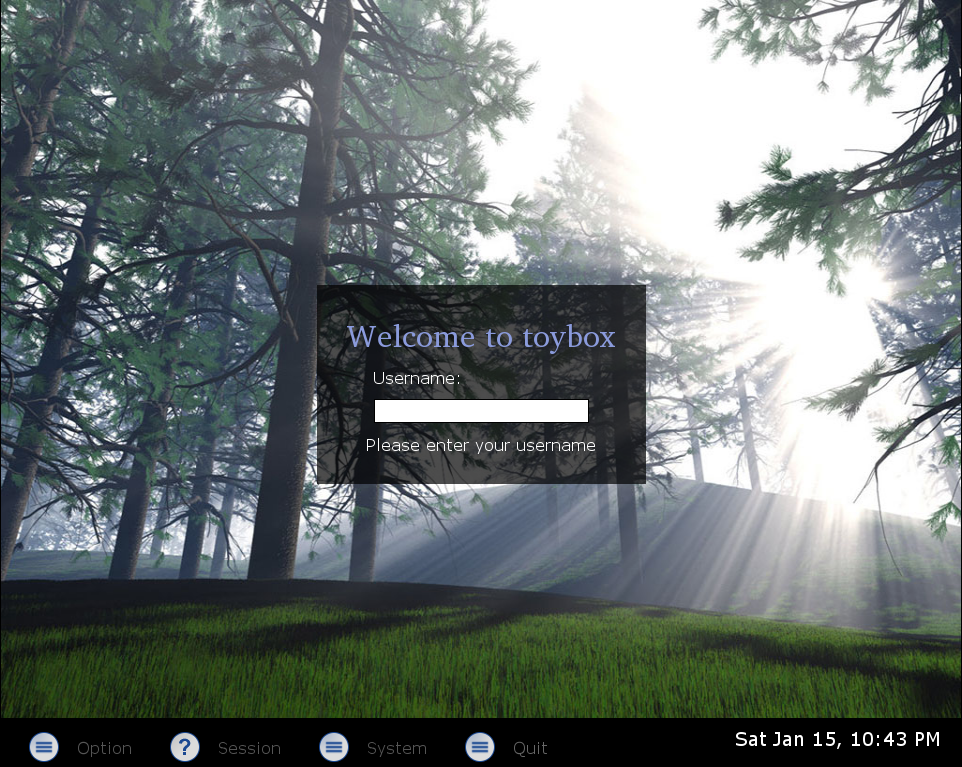
\includegraphics{gdm.eps}}
%\caption{˹�Ҩ���͡�ԹẺ��ҿ�ԡ}\label{fig:gdm}
\end{figure}

%\marginpar{\scalebox{.2}{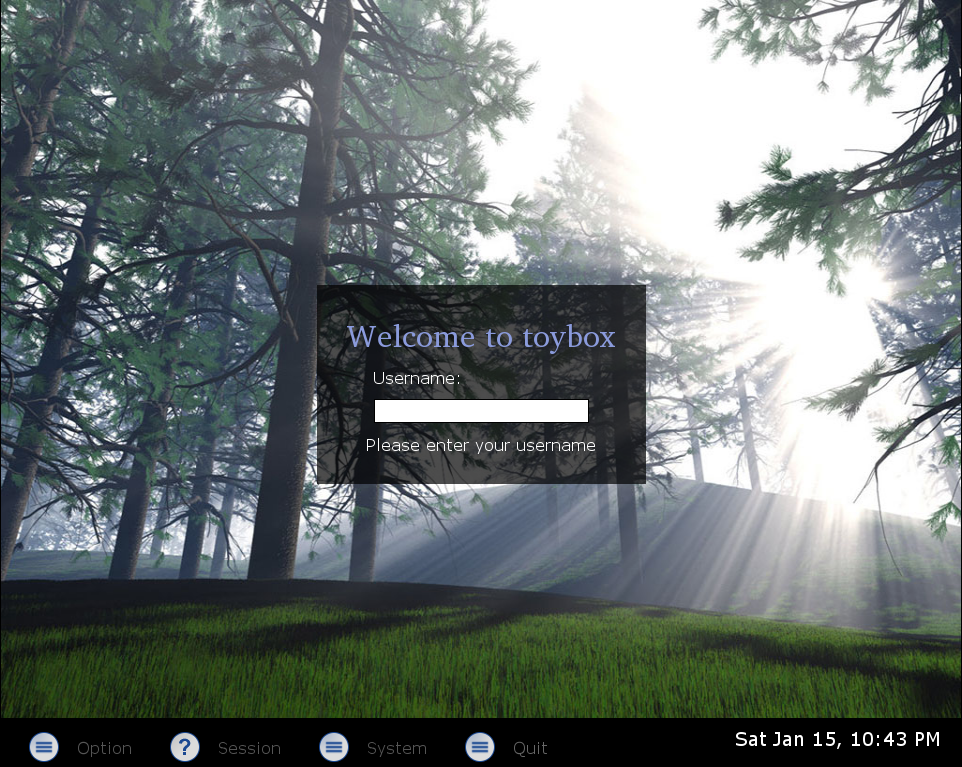
\includegraphics{gdm.eps}}}

��ҿ�ԡ������ҧ�ҡ�硫������ç����� \emph{X ��������� (X server)} %
������������鹰ҹ����Ѻ�к��Թ������Ѻ��������ҧ��ǹ��Сͺ�ͧ��ҿ�ԡ. ��ʷ�Ժ�Ǫѹ������ѡ�����к� Desktop Environment %
�� GNOME ���� KDE ���к�ഡ���ͻ�ҵðҹ���������ҹ. �к� desktop environment \myvocab{d}{Desktop Environment}{�к�, ��Ҿ�Ǵ��������ʹ͡�ҿ�ԡ�Թ����������Ѻ������·���Թ����������ҹ���դ�����ҡѹ������ٻ��ҧ˹�ҵ�����͹���ͤ���¡ѹ, �ӧҹ�����ѹ�� ���. ������ҧ Desktop Environment ���������� GNOME, KDE �繵�.}%
����ͧ����繵�ǨѴ��á�÷ء���ҧ�������ǡѺഡ���ͻ��˹�Ҩ���͡�Թ, ����, ���������Ѻ��ҹ�����Ẻ graphical user interface (GUI) %
\myvocab{g}{graphical user interface (GUI)}{�Թ������Ẻ��ҿ�ԡ����ʴ�˹�ҵ�ҧ, ������, ���� �ҧ˹�Ҩ�. ����������������ͤ������㹡����ͺ�ѹ�к�.}%
���. 㹡�ҿ�ԡ������������ҹ���дǡ�����硫�����, ��������ö�ѹ���������������·��������������Թ���੾�Тͧ����ͧ. ���ͧ�ҡ�к� GUI �����ٵ�ҧ������������, �������������¡Ѻ��������������ö���������ҧ����дǡ���.

��к� X �Թ���, �������������ҹ�ҧ\emph{�����Թ������������� (terminal emulator)} %
\myvocab{t}{terminal emulator}{\emph{�����Թ�������������}. ����������ͧ˹�Ҩ��ʴ��ŵ���ѡ��������Ѻ����. �����Թ��������������������������� X �Թ����� \cmd{xterm}, \cmd{gnome-terminal}, \cmd{konsole} �繵�.}%
���������� GUI �����ͧ���Ҿ�����ʴ��ź��к� X �Թ���. ����������Թ������������������»������ \cmd{xterm}, \cmd{gnome-terminal}, \cmd{konsole} �������Ѻ�����ͺ�ͧ͢�����. ���������ҹ�������������ԧ��ͺ��觨����ä���觷���͹����ҷҧ������촵���.


\begin{figure}[!tb]
\plfigure{.5}{sample_terminal.eps}{�����Թ������������ (\cmd{gnome-terminal}) ����ѹ�� X �Թ���}{terminalemu}
\end{figure}

�Թ������Ẻ CLI ��� GUI �ըش����Шش����ᵡ��ҧ�ѹ�. ���������ͧ��������¡�������͡�Թ��ҷҧ��ҿ�ԡ����. GUI �дǡ㹡�������������繷ء���ҧ����觷��Ѻ��ͧ����˹�ҵ�ҧ�, ����, ����. 㹷ҧ��Ѻ�ѹ��ʹչ����Ҩ�С����繢�ʹ������蹡ѹ. �����٢ͧ��á�зӷ��������������������§��, ������������������ջ���Է���Ҿ��§�ͷ����ѹ������������, �������ö�ӧҹ����ͧ������ѵ��ѵ������м�����ͧ��ͺ�Ѻ�������������. ����·��¡������ҧ仹������觷�����춹Ѵ. ����Ǥ������������ִ�Դ�Ѻ�ҹ���ҧ����ҧ˹��, �������ö�����觺�÷Ѵ�������������ѹ�ӧҹ੾�з����ҵ�ͧ�����. ����Ӥѭ�������ӧҹ����Ẻ�ԧ��ͺ���Ẻ�ѵ���ѵ�. �����������觢�鹵͹�ͧ�ҹ�����ҵ�ͧ��÷ӡ�����ö��¹\emph{����ʤ�Ի�� (shell script)} %
\myvocab{s}{shell script}{\emph{����ʤ�Ի��}. ������������觷�����������Ҵ��¡ѹ. ����еդ�������觷�����������鹺�÷Ѵ��ͺ�÷Ѵ. �дǡ����Ѻ�����觤ӷ���繢�鹵͹. ���ͧ�ҡ��������¡ó�, ����ö���ҧ�����, ����ö�Ǻ����������ҧ���֧��������Ҥ���������Ẻ interpreter ����. ����ʤ�Ի���պ��ҷ�Ӥѭ�Ѻ�Թء���ҡ�� ����ʤ�Ի����㹡������������������������ҧ�.}%
���ӧҹ���ѵ��ѵ���. ��ǹ��ʹ��¢ͧ����������дǡ㹡��������Ѻ������������. \mymemo{���������� ``����дǡ㹡��������Ѻ������������'' ᷹����� ``����дǡ㹡����'' �����繤�����ԧ�����Ҥ����ҡ���¢ͧ���������������ªԹ} ��Чҹ��������ҧ��ͧ��á����觷��͡�˹�ͨҡ\emph{�������硫� (text data)} %
\myvocab{t}{text data}{\emph{�������硫�}. �����ŷ���������������������ö��ҹ����������. �»á�Ԣ������硫�����¶֧�������¹���������ѧ��ɷ����ҹ��, ������ѡ��ФǺ��� (control character) �л�.}%
�蹡�õѴ����մ���, ��ô٢����ŷҧ��� �繵�. 


\subsection{�����͡�Թ�觵��������������}
\subsubsection{��͡�Թ��ҹ�͹��}
\emph{�͹�� (console)} ���¶֧�ش���������Ш��ʴ��ŷ�����µç�Ѻ����������. �����͡�Թ��ҹ�ҧ�͹���繡����͡�ԹẺ������������, ���繡����͡�ԹẺ�硫��������͡�ҿ�ԡ���������������������ö�ͧ����������㹡���ʴ���.
\subsubsection{��͡�Թ��ҹ�ҧ�������}
�����͡�Թ��������ҹ�ҧ������졷�������������� \cmd{telnet}, \cmd{ssh}, \cmd{X} ��� �Դ��͡Ѻ����ͧ�������������ͧ�����͡�Թ. �����͡�Թ��ҹ�ҧ�����������÷�����Ẻ�硫�������С�ҿ�ԡ��������\emph{���������ⵤ�� (network protocol)} ���ᵡ��ҧ�ѹ. ������ҧ������� \cmd{telnet} ������ⵤ�� telnet 㹡��������������ҧ����������, �����͡�ԹẺ��ҿ�ԡ������ⵤ�� xdmcp (X Disaplay Manager Control Protocol) �繵�. 


\section{����͡�ҡ�к�}
\subsection{�硫�����}
����͵�ͧ����͡�ҡ�к���������� ``\cmd{logout}''.\mymemo{����͡�ҡ�к��ͧ�к���Ժѵԡ�� Windows ���¡��� logoff ����š�ͧ�ٹԡ������¡��� logout}\refcmd{logout}


\cindex{logout}%
\begin{MyExample}[�����͡��ҷ�Ẻ�硫�����]
\begin{MyEx}
$ \cin{logout}
\arrowdown \thtt{�к���������˹�Ҩ�����͡����͡�Թ����}
login: \cursorprompt
\end{MyEx}
\end{MyExample}%$


����� \cmd{logout} ���з����������͡�Թ��ҹ��. �����������ͧ�����Թ������������������͡�Թ����֧������ \cmd{logout} �����, ��������� ``\cmd{exit}'' ᷹.\refcmd{exit}
\cindex{exit} ��觷��ᵡ��ҧ�ѹ�����ҧ \cmd{logout} �Ѻ \cmd{exit} ��� \cmd{logout} ����ҹ��������ͤ�ҵԴ������� \cmd{.bash\_logout} �������������á���ա�͹�Ш���÷ӧҹ�ͧ����. ��ǹ����� \cmd{exit} �Ш���÷ӧҹ�ͧ�������. �·�������ǡ�á����� \ovalbox{\cmd{Ctrl}}+\ovalbox{\cmd{d}} ������������繡�è���÷ӧҹ�ͧ�������蹡ѹ. \mymemo{\ovalbox{\cmd{Ctrl}}+\ovalbox{\cmd{d}} ���ѡ��ФǺ��������Թ�����¶֧����բ����Ź�����ա���� (end of file). ��觡����¶֧��è���÷ӧҹ�ͧ����.} 



\subsection{��ҿ�ԡ����}
��к� Desktop Environment ����������ѡ����Ѻ����������͡������͡��ҷ��͡�ҡ�к�.


\section{�����Թ������͹}
�»á�Ԥ���������˹������ͧ���դ͹��˹�觪ش. ����ͼ���餹˹����͡�Թ��ҹ�ҧ�͹��, ����餹��蹨��������ö������������騹���Ҽ��������͹����͡��ҷ�. ��ҵ�ͧ�����͡�Թ�������к����ǡѹ������ѹ, ����餹��蹵�ͧ��͡�Թ��ҹ�ҧ�������. �Թء��͹������ö��ѭ�ҹ���������觷�����¡���\emph{�����Թ������͹ (virtual terminal)}. %
\myvocab{v}{virtual terminal}{\emph{�����Թ������͹}. �����Թ����硫������ͧ�Թء��������ö����¹˹�Ҩ�������˹�Ҩ�������˹�Ҩͷ�����ٻ������§˹�Ҩ�����. �Ը�����¹˹�Ҩͷ����¡� \ovalbox{\cmd{Ctrl}} ��� \ovalbox{\cmd{Alt}} �����Ѻ�ѧ��ѹ����.}%
�����Թ������͹�Ш��ͧ�͹����������ªش��������ǡѹ. ���ҧ�á������ͧ�ҡ����������˹������ͧ���դ������, �������Ш��ʴ�����§˹�觪ش��ҹ��, ��������¹�͹�����������Թ������͹�����á����� \ovalbox{\cmd{Ctrl}} ��� \ovalbox{\cmd{Alt}} �����Ѻ\emph{��觪ѹ���� (function key)}. 

\begin{figure}[!htb]
\plfigure{.45}{virtual_terminal.eps}{�����Թ������͹}{virtual_terminal}
\end{figure}

\subsection{�������¹����}
�������Ҽ����ҹ���ѧ��͡�Թ���¡�ҿ�ԡ����������е�ͧ�������¹���硫�����, �����ҹ����ö�����¡����� \ovalbox{\cmd{Ctrl}}+\ovalbox{\cmd{Alt}}+\ovalbox{\cmd{F1}}\mymemo{\ovalbox{\cmd{Ctrl}}+\ovalbox{\cmd{Alt}}+\ovalbox{\cmd{F1}} ���¤��������顴���� \ovalbox{\cmd{Ctrl}} ��� \ovalbox{\cmd{Alt}} ��ҧ������ǡ����� \ovalbox{\cmd{F1}} ���. ��硫���������ͧ������ \ovalbox{\cmd{Ctrl}} ����������͹�ѹ.} �������¹�������Թ�ŷ�� 1 (���ٻ��� \ref{fig:virtual_terminal} ��Сͺ). ������ \ovalbox{\cmd{Ctrl}}+\ovalbox{\cmd{Alt}}+\ovalbox{\cmd{F2}} ��������¹�������Թ�ŷ�� 2 ������硫������蹡ѹ. ��Ҩ�����¹��Ѻ�繡�ҿ�ԡ��������͹�����顴���� \ovalbox{\cmd{Ctrl}}+\ovalbox{\cmd{Alt}}+\ovalbox{\cmd{F7}}. 

�»á������ X �����������ѹ�������������Щй�������Թ�ŷ���繡�ҿ�ԡ�������������Թ�ŷ�� 7 (\cmd{F7}) ��ҹ��. ����� X ����������ѹ�����ҡ����˹�觵��, X ����������Ƿ���ͧ���ѹ������͹�ŷ�� 8 (\cmd{F8}) �繵�.

������ҧ����������Թ������͹�� ��� �. ������������ѹ������ӹdz��觡Թ�����繪���������������͡�Թ��ҧ���. ��� �. �ո��д�ǹ��ͧ��ҹ������������դ�������������������͡�Թ��ҹ�ҧ��������. ����繤�����������������Թء�� ��� �. ��ͧ��͡��ҷ���������� �. �����������. 㹡óչ���� �. �����繵�ͧ��͡��ҷ��͡�ҡ�к�, ��§�����¹�������Թ������͹�繵���������� �. ������Ǥ����·������ռš�з��Ѻ�����������ͧ�ѹ����. ����͹�� �. ��ҹ���稡�����¹�����Թ������͹��Ѻ�繵���������� �. ���ա��. ������ҧ����������Թ������͹������ �������¹�ҡ��ҿ�ԡ�������硫��������ҡ�ҿ�ԡ�����ջѭ���������ö�Ѻ�����Ũҡ������������������. 

\section{�������ͧ��}\mymemo{���¤����㨼Դ�����������������͹ DOS (Disk Operating System). 㹤����繨�ԧ���� DOS ����к���Ժѵԡ���������������. ����������� DOS ���Թ������ CLI �֧����餹����令Դ���������� DOS ����͹�ѹ.}
㹻Ѩ�غѹ�֧�������Թ������Ẻ��ҿ�ԡ���繷������ѹ���ҧ���ҧ��ҧ����������¤�������Թ������Ẻ��÷Ѵ�����������������. �������������Թ�����ʷ����ͺ�Ѻ����������������������鹾������С���ʴ����繵���ѡ������ѡ. ���ͧ�ҡ������ͧ��þ�鹰ҹ�ͧ���������鹾������Ш��Ҿ�������ö�ʴ�����ѡ��, �����������������������繵�ͧ�շ�Ѿ�ҡ��ҡ������. ����ʴ����繵���ѡ��, ��ͤ�����������ҷ��������������ѹ��. ����Ѻ��������¡Ѻ�鹾��������ö��觤�������Ǵ������������º��º�Ѻ����������. %
\mymemo{��������������Ҫ�ҡ��ҡ�����鹾�������м�����ͧ��зӡ�����¢�鹵͹���� ����͹�����, ��秨ش�ͧ��������ç�Ѻ���˹觷���ͧ���, �������, ���͡���� ���. ��Ҽ�����ҧ���˹觹�����١��ͧ��Шӵ��˹觢ͧ�����ҧ���������ҡ. �����º���ҡ�����¹�������, ��������������¹�����¡��ҡ�����¹���鹾����.}
��з���Ӥѭ����ش��ͼ��������ö��¹������繢�鹵͹���Ǵ��Թ��÷�������Ẻ�ѵ��ѵ�. �����˵ؼ�����ҹ���ͧ������������è��֡�ҡ�����������ҧ��ԧ�ѧ���ͷ����繾�鹰ҹ㹡�����Թء�����. 

��к���Ժѵԡ���ٹԡ���ؤ�á�����������¡�ѹ��� Bourne shell (\cmd{sh})\mymemo{��к��Թء�� \cmd{sh} ���� symbolic link �ͧ \cmd{bash}.} ��觵�駪��͵��������ҧ��͹�� Stephen Bourne. ��ѧ�ҡ����Դ BSD �ٹԡ��, Bill Joy �����ҧ������������ó����¡Ѻ���ҫ�����դ�������ö������ҡ��鹡���������¡��� C shell (\cmd{csh}). �͡�ҡ����ѧ���������µ���Դ����� Korn shell (\cmd{ksh}), Bourne-again shell (\cmd{bash}), Zsh (\cmd{zsh})\mymemo{``z'' � zsh �դ�������ὧ���¶֧�������ش����. zsh ���������Ǻ�����觴��ͧ�����ҧ�����ѹ����ըش���������������շ���ش㹺�ô�����������.} ���. ��к���Ժѵԡ���Թء�����͡�� Bourne-again shell, ���ͷ�����¡������� \cmd{bash} �����������. Bash �������˹�����ਤ GNU. Bash ���ҧ����� Brain Fox ��� Chet Ramey ����դ�����ҡѹ��Ѻ Bourne �����ըش��㹡����䢺�÷Ѵ�����, �����ͺ�Ѻ�����, ��������������������� ���.

����Ѻ�к���Ժѵԡ�õ�С���ٹԡ��, ��������������觤�������������������������ŷӧҹ�¼�ҹ����. ���˵ط�����¡����������������˹�ҷ�������͡�����繵�ǡ�ҧ�����ҧ��������м����. 㹷ҧ��ɮ�, ������\emph{������ä���� (command interpreter)} ���ҧ˹�觷���դس���ѵ�\emph{�ԧ��ͺ (interactive)} �Ѻ�����, �դ�������ö�Ǻ�����ô��Թ�ҹ, �Ѻ����ë���Ҩ���繤�ҷ������ҡ����������ͪ�������觵����������, ���¡��зӡ���������ҧ�, �Ѻ����觢��������Ѻ�����������¡���繵�. 

\emph{����� (command)} %
\myvocab{c}{command}{\emph{�����}. �����͵���ѡ�÷������ҧ�鹾�����觵����������Ť���������С�зӡ�õ���. �������·�����ѧ���¶֧��������ͪ��������������¡���ҹ����.}
��������ä���㹷�����Ҩ�����¶֧����觷����������ö��зӡ���ͧ�������¡���\emph{��������� (shell built-in command)} %
\mymemo{������ҧ����������� \cmd{cd}, \cmd{pwd}, \cmd{fg} �繵�. ������ҧ�������¹͡����������������� \cmd{ls}, \cmd{cp}, \cmd{rm} ���.}%
���ͤ���觷�������������ö��зӡ�����ͧ���¡���\emph{�������¹͡ (external shell command)} ��觡���\emph{����� (program)} ����ͧ. 

\subsection{�ѡ���}
�ѡ��� (character) \mymemo{�ѡ������¶֧����ѡ������֧����ͧ���µ�ҧ�.}������������������»á�������ѡ�������ѧ��ɷ�����¡����ѡ��� ASCII (American Standard Code for Information Interchange) ����ʴ�㹵��ҧ��� \ref{tab:ascii} (˹�� \pageref{tab:ascii}). �ѡ��� ASCII �ѧ������\emph{�ѡ��ФǺ��� (control character)}\mymemo{���ͧ�ҡ�ѡ��ФǺ�������ҹ��������ٻ��ҧ˹�ҵ�, �ҧ���駨֧���¡��� non-printable character.} ����Ѻ�Ǻ�����û����żŢ��������ͤǺ�������觢�����, ���\emph{�ѡ��С�ҿ�ԡ (graphic character)} ������ѡ��з�����������ͧ������������ѡ�������ѧ�������֧����ͧ���µ�ҧ���������.

%���͡���ͧ����������ѡ��з���ʴ��ҧ˹�Ҩ��� (printable character) �Ѻ�ѡ��з���������ö�ʴ��ҧ˹�Ҩ��� (non-printable character). �ѡ��з���ʴ��ҧ˹�Ҩ��������ѡ��з������ҡ���������������ö�����觷�������������͡����� \ovalbox{\texttt{a}} ��л�ҡ�����ѡ�� ``a'' �ҧ˹�Ҩ�. ��ǹ�ѡ��з���������ö�ʴ��ҧ˹�Ҩ���������͡����� \ovalbox{\texttt{Enter}} ���繡�������������Ť���觷�������. �ѡ��з�������������ҹ���·��������


%�ѡ��з���������ö�ʴ��ҧ˹�Ҩ����ժ������¡�ա���ҧ���\emph{�ѡ��ФǺ��� (control character)} . ������ҧ���������ö������ \ovalbox{\texttt{BackSpace}} ����ź�ѡ��з�����������. ��á����� \ovalbox{\texttt{BackSpace}} ��ԧ������繡�����ѡ��� BS ������ѡ��ФǺ��������ŷ���������. �ҡ���ҧ \ref{tab:ascii} (˹�� \pageref{tab:ascii}) ������������������ö������ѡ��з���������¤������. ������������ҡ���դ�������Ѻ�ѡ��ФǺ�������������ҹ���� \kk{BackSpace}, \kk{Delete}, \kk{Tab}, \kk{Enter} �繵�. 㹡óշ������������դ�������ҹ��, ���������ö������ C-h ᷹ \ovalbox{\texttt{BackSpace}}, C-m ᷹ \ovalbox{\texttt{Enter}} ��. �͡�ҡ����ҡ� C-d (EOT) ����ж���������բ����Ź�������ǨШ���÷ӧҹ�»�����. ����� C-h, C-m, C-d ����繡�õդ����ͧ�ѡ�����дѺ�����Թ��. ����Ǥ���������ҡ� C-h ���������Թ�Ũ��ŧ���ѡ��� BS ������������. 



�·����, ���������ö������ѡ��С�ҿ�ԡ����¤������. ���ѡ��ФǺ����������ºҧ�����ҹ�鹷������ö�����ҡ����������µç�� \kk{Backspace} \kk{Tab} \kk{Enter} �繵�. 㹡óշ�������촷��������դ������ɴѧ�����, �������ö������ \kk{Ctrl} ��ҧ������ǡ��������ѡ�������ѧ��ɵ���������ҧ�ѡ��ФǺ�����. ������ҧ�� \kk{Ctrl}+\kk{h} ��᷹ \kk{Backspace}, \kk{Ctrl}+\kk{i} ��᷹ \kk{Tab} ��� \kk{Ctrl}+\kk{m} ��᷹ \kk{Enter} �繵�.


�ѡ��ФǺ����ҧ����դ������¾���ɵ�������Թ����������. ������ҧ���ѡ��� EOT (\underline{E}nd \underline{O}f \underline{T}ransmission) %
\mymemo{��ҧ�����¡ EOT ��� EOF (\underline{E}nd \underline{O}f \underline{F}ile).}%
���¶֧����ش�����Ź����. ���������ö���ѡ��ФǺ�������¡����� \kk{Ctrl}+\kk{d} �������������ͨ���÷ӧҹ�ͧ����. ��á����� \kk{Ctrl}+\kk{l} �����¶֧ FF (\underline{F}orm \underline{F}eed) ����դ������¶֧��â��˹������. 㹡óչ����觷���ʴ���˹�Ҩ�����Ǩж١ź��� (������) ���Ǩ���������������������÷Ѵ�������. ���ҧ��� \ref{tab:controlterm} �ʴ��ѡ��ФǺ�����������. 

\bigskip
\tablecaption{�ѡ��ФǺ�������դ������¾���ɵ�������Թ����������}\label{tab:controlterm}
\tablefirsthead{\hline \multicolumn{1}{c|}{�ѡ��ФǺ���} & \multicolumn{1}{|c|}{����} & \multicolumn{1}{|c}{��͸Ժ��}\\
\hline
}
\tablehead{\multicolumn{3}{l}{{\slshape ��ͨҡ˹�ҷ������}}\\ \hline \multicolumn{1}{c|}{�ѡ��ФǺ���} & \multicolumn{1}{|c|}{����} & \multicolumn{1}{|c}{��͸Ժ��}\\
\hline
}
\tabletail{\hline \multicolumn{3}{r}{\slshape ���˹�ҶѴ�}\\}
\tablelasttail{\hline}
\begin{supertabular}{c|c|p{.5\textwidth}}
%SOH & \kk{Ctrl}+\kk{a}  & ����͹��������价��鹺�÷Ѵ, ��᷹ \Ovalbox{Home} ��\\
%SOT & \kk{Ctrl}+\kk{b}  & ����͹������������ѧ˹�觵���ѡ���, ��᷹ \kk{\myleftarrow} ��\\ 
ETX & \kk{Ctrl}+\kk{c} & �ѭ�ҳ SIGINT (interrupt) ¡��ԡ��÷ӧҹ�ͧ�����\\
EOT & \kk{Ctrl}+\kk{d} & ����ش�����Ź����, ����÷ӧҹ㹡óշ�����ѡ��ФǺ�������繵���á����������\\
 &  & ź����ѡ�÷������ç��������㹡óշ��������������, ��᷹ \Ovalbox{Del} ��\\
%ENQ & \kk{Ctrl}+\kk{e}& ����͹��������价����º�÷Ѵ, ��᷹ \Ovalbox{End} ��\\
%ACK & \kk{Ctrl}+\kk{f} & ����͹��������仢�ҧ˹��˹�觵���ѡ���, ��᷹ \kk{\arrowright} ��\\
%BEL & \kk{Ctrl}+\kk{g} & ��д������¡��ԡ��èѴ���÷Ѵ\\
%BS & \kk{Ctrl}+\kk{h} & ź�ѡ��з������˹����������˹�觵��, ��᷹ \Ovalbox{Backspace} ��\\
%VT & \kk{Ctrl}+\kk{k} & ź�ѡ��е������������仨��ش��÷Ѵ\\
%FF & \kk{Ctrl}+\kk{l} & ������˹�Ҩ�\\
%CR & \kk{Ctrl}+\kk{m} & ����÷Ѵ, ��᷹ \Ovalbox{Enter} ���� \Ovalbox{Return} ��\\
%SO & \kk{Ctrl}+\kk{n} ���� \kk{arrowdown} & ����ѵԤ���觶Ѵ�\\
%DLE & \kk{Ctrl}+\kk{p} ���� \kk{arrowup} & ����ѵԤ���觡�͹˹�ҹ��\\
DC1 & \kk{Ctrl}+\kk{q} & �ʴ��ŷҧ˹�Ҩ��ա������ѧ�ҡ���١��ش�����ѡ��ФǺ��� DC3 \\
%DC2 & \kk{Ctrl}+\kk{r} & ���һ���ѵԤ������͹��ѧ\\
DC3 & \kk{Ctrl}+\kk{s} & ��ش����ʴ��ŷҧ˹�Ҩͪ��Ǥ��� (�������Ѻ�����Թ�ŷ����)\\
SUB & \kk{Ctrl}+\kk{z} & �ѭ�ҳ SIGSTOP (stop) ��ش��÷ӧҹ�ͧ�����(���Ǥ���)\\
\end{supertabular}
\bigskip





%㹡�÷ӧҹ�дѺ�����������ö�觻������ͧ�ѡ�����ѧ���.
%
%\begin{itemize}
%\item blank: ���� SP ��� TAB ���繵���������ҧ��.
%\item control operator: ���� CR, NL, ``||'', ``\&\&'', ``\&'', ``;'', ``;;'', ``|'', ``(``, ��� ``)'' �繵���ѡ��ФǺ�����ô��Թ����觢ͧ����. 
%\item metacharacter: ���� blank ���� ``|'', ``\&'', ``;'', ``(``, ``)'', ``<'', ``>'' ����繵���觤����������� quote. \mymemo{��� quote ���¶֧���������ͧ���� double quote ���� single quote �ӡѺ.}
%\item wildcard: ��㹡���кت������, ��������ͧ���� ``*'' ᷹�ѡ���������ٹ���Ǣ���. ����ͧ���� ``?'' ᷹�ѡ�������˹�觵����ҹ��. ���������ͧ���� ``*'' ���� ``?'' ����� quote ��������դ����� wildcard.
%
%
%\item escape: ���� ``\bs'' �������˹���ѡ��о������������������դ�������Ẻ�ѡ�������ҹ��, ��������ѡ��и�����. ������ҧ��
%\end{itemize}


\subsection{�����}
����觤����觷���ͧ���������������ӧҹ. ��Ҥ�����������������������, ����Ҩ����觤������ѧ���仹��.

\begin{MyVerbatim}
{\thaitext\it ���Ҿ�Ǵ��������˹�} {\thaitext\it ������觷�����(������)} {\thaitext\it Ẻ���(�����ҧ��)} {\thaitext\it �����������ŵ��仹��}
\end{MyVerbatim}

�����觤������������������ѡɳФ���¡Ѻ�����觤���觴����Ҩ������ٻẺ�����觤���觷������\mymemo{����ͧ���� \myenter{} ���ʴ��֧��á����� \kk{Enter} �������ͧ���� \cmd{\char32} �ʴ��֧��ͧ�.}

%\begin{figure}[!htb]
%\caption{�ٻẺ�����觤����}
%\begin{MyVerbatim}
%{\thaitext\textbf{Ẻ����:}}
%$ {\thaitext\textbf{�����}}\char32{\thaitext\textit{�����������}}\char32{\thaitext\textit{�����������}}\char32... \myenter
%{\thaitext\textbf{Ẻ�����:}}
%$ {\thaitext\textit{�������Ҿ�Ǵ����=���}}\char32{\thaitext\textit{�������Ҿ�Ǵ����=���}}\char32...\char32{\thaitext\textbf{�����}}\char32{\thaitext\textit{�����������}}\char32{\thaitext\textit{�����������}}\char32... \myenter
%\end{MyVerbatim}
%\end{figure}


\begin{MyVerbatim}
$ {\thaitext\textit{�������Ҿ�Ǵ����=���}}\char32{\thaitext\textit{�������Ҿ�Ǵ����=���}}\char32...\char32{\thaitext\textbf{�����}}\char32{\thaitext\textit{�����������}}\char32{\thaitext\textit{�����������}}\char32... \myenter
\end{MyVerbatim}

��ǹ������㹡����觤����������ͤ����. ��ǹ����� ``\textit{�������Ҿ�Ǵ����=���}'' ��� ``\textit{�����������}'' ������������ա���. 

������»á�Ԩ��� ``��'' �����ѧ���. ��㹷�������¶֧��ù��ѡ�������ѧ��������§�ѹ����Ҩ������դ������¡���. ��㹷�����ѧ���¶֧������ѡ�÷��������ª�ͧ���������� \cmd{abc def} �ж��������ͧ�Ӥ�� \cmd{abc} �Ѻ \cmd{def}. �����ѧ�¡��Ф���ᵡ��ҧ�����ҧ����ѡ�������ѧ��ɵ����� (small letter) ��е���˭� (capital letter) ����.\mymemo{�����աẺ�ͧ����ѡ�������ѧ��ɵ����硤�� lower-case letter. ��Ъ��ͧ͢����ѡ�������ѧ��ɵ���˭��� upper-case letter.}

����ͼ���顴���� \Ovalbox{\cmd{Enter}} ����, ����е�Ǩ�ͺ��Ҥӷ��������仹��������, �����������ö�դ������зӧҹ��������觵���. ����ͧҹ������仨����º���������������ʴ�������������ͷ����Ѻ����觶Ѵ�����������Ѱ�ѡõ���ٻ��� \ref{fig:shell_circle}.

\begin{figure}[!htb]
\plfigure{.5}{shell_circle.eps}{ǧ�á���ѹ����觢ͧ����}{shell_circle}
\end{figure}

��觷������˹�Ҥ���� (������������) ����\emph{�������Ҿ�Ǵ���� (environment variable)} ��Ф�Ңͧ����ù���. ����ѧࡵ��ҵ������Ф�Ңͧ����â�鹴�������ͧ������ҡѺ�·���ҧ˹����Т�ҧ��ѧ����ͧ������ҡѺ����ժ�ͧ�. �·����������觤�����ѡ������кص������Ҿ�Ǵ������Ф��Ẻ���, ¡���㹡óշ���ͧ����кص������Ф�Ңͧ�����������觷���ͧ�������Ѻ���੾�Ф��� (������ҧ��� \ref{ex:enveffect}). 

��觷������Ѵ�ҡ��������¡���\emph{����������� (argument)}\gindex{argument}\gindex{�����������} �Ҩ����\emph{������͡ (option)}\gindex{option}\gindex{������͡}, ��������ͤ�ҷ���ͧ������������, ��������繵�. ���������������������觴���\emph{��ͧ� (space)} ����\emph{�ش������� (tab)}. ��ѧ�ҡ����������觷���ͧ���������顴���� \cmd{\ovalbox{Enter}} ��зӡ��. 

������ҧ���仹���ʴ������觤���觵�ҧ������.%
\cindex{pwd}%
\cindex{ls}
\cindex{echo}


\begin{MyExample}[�����觤���觼�ҹ�ҧ����]\label{ex:commands}
\begin{MyEx}
$ \cin{pwd}   \shabox{\myleftarrow{} \thtt{�����觤����������}}
/home/somchai
$ \cin{ls}   \mycomment{�����觤����������}
Desktop  file1
$ \cin{/bin/ls}   \mycomment{��觤�������кط������ͧ����������� (full path)}
Desktop  file1
$ \cin{../../bin/ls}\mycomment{��觤�������кط������ͧ�������º�Ѻ���˹觻Ѩ�غѹ}
$ \cin{ls -l}   \mycomment{�����觤���觡Ѻ����������� (������͡)}
total 4
drwxr-xr-x    2 somchai  somchai      4096 Mar 17 22:36 Desktop
-rw-rw-r--    1 somchai  somchai         0 Apr  4 23:06 file1
$ \cin{LANG=th_TH ls -l}   \mycomment{����кص������Ҿ�Ǵ����੾�Ф���}
total 4
drwxr-xr-x    2 somchai  somchai      4096 \thtt{��.�.} 17 22:36 Desktop
-rw-rw-r--    1 somchai  somchai         0 \thtt{��.�.}  4 23:06 file1
$ \cin{echo $PATH}
/usr/bin:/bin:/usr/X11R6/bin
$ \cursorprompt
\end{MyEx}
\end{MyExample}
%$ \cin{cal}
%     {\thaitext ����¹} 2003
%{\thaitext ��} {\thaitext �.} {\thaitext �.} {\thaitext �.} {\thaitext ��} {\thaitext �.} {\thaitext �.}
%       1  2  3  4  5
% 6  7  8  9 10 11 12
%13 14 15 16 17 18 19
%20 21 22 23 24 25 26
%27 28 29 30
%$ \cin{echo $LANG}
%th_TH.TIS-620

�����觤���觷����¾������ͤ��������� ``\cmd{ls}'' ���������к���á���� (�������) �ͧ����觷���ͧ�����觴����� ``\cmd{/bin/ls}'' ���� ``\cmd{../../bin/ls}''. 㹡óշ����������ͤ�������ҧ����, ����Ф��ҵ������� (�����) �ҡ\emph{�������Ҿ�Ǵ���� (environment variable)} ������ \cmd{PATH}. ��Ңͧ�������Ҿ�Ǵ���� \cmd{PATH} �繪�����á���յ�ҧ���������������鹴��µ���ѡ�� ``\cmd{:}''. �������觤����������к���á������ \cmd{ls} ����, ����е�Ǩ�ͺ��� \cmd{ls} �繤���������������. ���������繤�������㹡���ҵ������� \cmd{ls} �ҡ��á���� \cmd{/usr/bin}, \cmd{/bin} ��� \cmd{/usr/X11R6/bin} ����ӴѺ. 

�����觤�������к���á��������ö���͡�� 2 Ẻ��͡���к���á���բͧ����������������ͧ�����Ẻ \emph{full path}\gindex{full path} ���Ẻ \emph{relative path}\gindex{relative path}. ������ҧ�ͧ����к������Ẻ full path ���� \cmd{/bin/ls} �繡���к���á���շ����������\emph{�ٷ��á���� (root directory)} (\cmd{/}), \cmd{bin} ���֧����������觡������亹��յ���ӴѺ. ��ǹ����кط������ͧ�����Ẻ relative path ����ҧ�ԧ�ҡ��á���շ��ӧҹ��������ش ``\cmd{.}'' ᷹��á���շ��ӧҹ��������� ``\cmd{..}'' ᷹��á���շ�������˹����á���ջѨغѹ����˹�觢��. �ѧ��鹨ҡ������ҧ��� \ref{ex:commands}, \cmd{../../bin/ls} �֧�繡���к������ \cmd{/bin/ls} ������á���շ��ӧҹ����͹��鹤�� \cmd{/home/somchai}. 

�������������������������á���շ��ӧҹ������� \cmd{a.out}\mymemo{\cmd{a.out} �繪��������Ѿ������ҡ��ä����������. ��ҡѹ��Ҫ��͹������ Dennis Ritchie �����¹���� C ���¶֧ ``the output of the assembler'' �֧��������������ҧ�ҡ���������ʵ鹩�Ѻ��� \cmd{a.out}.} ��е�ͧ��è��ѹ��������. ��ҵ�ͧ�кش������ \cmd{a.out} �������˹���� relative path ���������ҧ���仹��
\begin{MyExample}[����ѹ���������������á���շ��ӧҹ����]
\begin{MyEx}
$ \cin{ls -l a.out}
-rwxr-xr-x    1 somchai  users          28 Apr 28 20:48 a.out
$ \cin{a.out}
-bash: a.out: command not found
$ \cin{./a.out}
Hello world.
\end{MyEx}
\end{MyExample}%$
�������ͧ��þ���� ``\cmd{./}'' ������������ش (\cmd{.}) ������¶֧��á���շ��ӧҹ�������㹵������Ҿ�Ǵ���� \cmd{PATH} ����.

\subsection{��Ǩ�ͺ�������ͧ�����}
���������й��������Ҥ���觷����ѹ������͡�� 2 �������˭���������觻�Сͺ�����������������. ����� bash ���դ���觻�Сͺ���� \cmd{type}\cindex{type}\refcmd{type} ������Ѻ��Ǩ�ͺ����Ҥ���觷������仹���繤���觻������. 

\begin{MyExample}[��Ǩ�ͺ�����������.]
\begin{MyEx}
$ \cin{type cd}
cd is a shell builtin
$ \cin{type ls}
ls is aliased to `ls --color=auto -F'
$ \cin{type /bin/ls}
/bin/ls is /bin/ls
\end{MyEx}
\end{MyExample}%$

�ҡ������ҧ�������������Ҥ���� \cmd{cd} �繤���觻�Сͺ��������, �����������ö�ӧҹ��ѹ������ͧ��ҹ���亹��ըҡ���촴ԡ�����ǡ�зӡ��. �͡�ҡ��鹷������������Ҷ����觤���� \cmd{ls} �����������¶֧ ``\cmd{ls --color=auto -F}''\mymemo{������ͧ����ǡѺ alias ����˹�� \pageref{sec:alias}.}, ������觤�������� \cmd{/bin/ls} ���繡����Ŵ���������� \cmd{/bin/ls} �ҡ�з��µç������ա����������͡��.

\subsection{�������Ҿ�Ǵ����}
\emph{�������Ҿ�Ǵ���� (environment varible)}\gindex{environment variable}\gindex{�������Ҿ�Ǵ����} ��\emph{��������� (shell variable)}\gindex{shell variable}\gindex{���������} ����������纤�����͢����źҧ���ҧ������������ͧ����ռŵ�������������¡��ҡ�����鹴���. ������ҧ�蹵������Ҿ�Ǵ���� \cmd{PATH} �繵���÷���纤�Ңͧ��á���շ�����������ҧ��������Ф��Ҥ���觨ҡ��á��������ҹ������ͼ����������ͤ��������������. 


��á�˹��������Ҿ�Ǵ������Ф�Ңͧ����÷�����������ͧ���� ``\cmd{=}'' ��������� \cmd{export}\cindex{export} ��С��������ù���繵������Ҿ�Ǵ����.\refcmd{export} ����͵�ͧ����ʴ���Ңͧ����ù����������ͧ���´������ (\cmd{\$}) ��˹�Ҫ��͵�����繡����ҧ�ԧ���.\mymemo{���ͤ����Ѵਹ㹡���ʴ���Ңͧ�����, �ҧ�����Ҩ��������ͧ����ǧ��纻ա�� (\cmd{\{\}}) �ӡѺ���� �� \cmd{\$\{PATH\}}}
\begin{MyExample}[��õ�駤�ҵ������Ҿ�Ǵ����]
\begin{MyEx}
$ \cin{PATH=/bin:/usr/bin:/usr/local/bin}
$ \cin{export PATH}
$ \cin{echo $PATH}
/bin:/usr/bin:/usr/local/bin
\end{MyEx}
\end{MyExample}
��÷Ѵ \cmd{PATH=/bin:/usr/bin:/usr/local/bin} �繡�á�˹���е�駤�ҵ����. ��ǹ����� \cmd{export} �з�������÷���˹�����繵������Ҿ�Ǵ����. ��Ҽ���������觤���� \cmd{export} ����÷����仨ж���繵���ø����������. ����ᵡ��ҧ�����ҧ�������Ҿ�Ǵ�����Ѻ�������������������ͤ���觷���зӡ����������������Ѻ��� (�׺�ʹ) ���͵������Ҿ�Ǵ������Ф�Ңͧ�ѹ����. 㹷ҧ��Ѻ�ѹ, ��������ͤ���觷���з�����������鹨�������ѡ�Ѻ����������������������������Ҿ���� (�׺�ʹ���������������������������). ���������ö��駤�ҵ������Ҿ�Ǵ����������˹�觺�÷Ѵ�ѧ���.
\begin{MyExample}[��õ�駤�ҵ������Ҿ�Ǵ�������㹺�÷Ѵ����]
\begin{MyEx}
$ \cin{export PATH=/bin:/usr/bin:/usr/local/bin}
\end{MyEx}
\end{MyExample}
�����觤���� \cmd{export} ���ҧ���Ǩ��繡���ʴ��������Ҿ�Ǵ��������������������.

�»á��, ����к��е�駤�� \cmd{PATH} �»�������������������. ������ѧ���ҵ�駤�� \cmd{PATH} ������µ���ͧ�����Ҩ�з����ź��� \cmd{PATH} ������������Ƿ����������������ҧ���ҧ�����. 㹡óշ���ͧ���������á���բͧ�����ŧ㹵������Ҿ�Ǵ���� \cmd{PATH} ��èзӵ��������ҧ���仹�������ѡ�ä������ͧ�����. ����Ǥ�;������á���շ���ͧ���������ҹ��, ����ͧ���á�����ͧ������.

\begin{MyExample}[�������������������Ҿ�Ǵ���� \cmd{PATH}]
\begin{MyEx}
$ \cin{echo $PATH}
/usr/bin:/bin:/usr/X11R6/bin
$ \cin{export PATH=$PATH:/home/somchai/bin}
$ \cin{echo $PATH}
/usr/bin:/bin:/usr/X11R6/bin:/home/somchai/bin
\end{MyEx}
\end{MyExample}


����ͼ�����ѹ���������������, ���������ѹ��鹨��׺�ʹ����Ѻ���������Ҿ��Ҿ�Ǵ�����ҡ�������ѹ����觹�鹴���. ��������ѹ��������ҧ���ǡѹ��������յ������Ҿ�Ǵ������ҧ�ѹ�ռŵ�ҧ�ѹ. ������ҧ�蹵������Ҿ�Ǵ���� ``\cmd{LANG}'' ���繵�Ǻ͡��Ҿ�Ǵ�����ͧ���ҷ��������. �ռŷ�������ʴ���������������ѡ�������Ҿ�Ǵ�������. ������ҧ��.\mymemo{������ҧ�������Թ�ŷ���ʴ�����������}\refcmd{date}


\begin{MyExample}[�š�з��ͧ��ҵ������Ҿ�Ǵ������ͤ���觷����]
\begin{MyEx}
$ \textcolor{blue}{export LANG=en\_}\cin{US}
$ \cin{date} \mycomment{��Ҿ�Ǵ���������ѧ���}
Wed Oct  8 01:15:31 JST 2003
$ \textcolor{blue}{export LANG=th\_}\cin{TH.TIS-620}
$ \cin{date} \mycomment{��Ҿ�Ǵ����������}
\thtt{�. 8 �.�. 2546 01:16:23 JST}
\end{MyEx}
\end{MyExample}%$
Bash �����դس���ѵԾ���ɷ������ö��Ш���Ҿ�Ǵ����੾�Ф���觷���ͧ�����. ������ҧ���仹���繡���ʴ��ѹ��͹����������㹢�з����Ҿ�Ǵ�����ͧ��������觤���觹���������ѧ���. 
\begin{MyExample}[�š�з��ͧ��ҵ������Ҿ�Ǵ������ͤ���觷����੾�Ф���]\label{ex:enveffect}
\begin{MyEx}
$ \cin{export LANG=C}
$ \cin{date}
Sun Oct 12 13:57:23 JST 2003
$ \textcolor{blue}{LANG=th\_}\cin{TH.TIS-620 date} \mycomment{�к���Ҿ�Ǵ����������੾�Ф���}
\thtt{��. 12 �.�. 2546 13:58:00 JST}
$ \cin{date}
Sun Oct 12 13:59:05 JST 2003
\end{MyEx}
\end{MyExample}
�ҡ������ҧ�ѧ����Ǩ��������ҡ�þ���� \cmd{LANG=th\_TH.TIS-620} ˹�Ҥ���觷����觨�����੾�Ф���觹���. �Ըա�ôѧ������ջ���ª������͵�ͧ����к���Ҿ�Ǵ�������Ǥ���������觷���ͧ���.

\begin{center}
\bigskip
\tablecaption{�������Ҿ�Ǵ���������}\label{tab:environment_variables}
\tablefirsthead{\hline \multicolumn{1}{c|}{�������Ҿ�Ǵ����} & \multicolumn{1}{|c}{��͸Ժ��} \\
\hline
}
\tablehead{\multicolumn{2}{l}{{\slshape ��ͨҡ˹�ҷ������}}\\ \hline \multicolumn{1}{c|}{�������Ҿ�Ǵ����} & \multicolumn{1}{|c}{��͸Ժ��} \\
\hline
}
\tabletail{\hline \multicolumn{2}{r}{\slshape ���˹�ҶѴ�}\\}
\tablelasttail{\hline}
\begin{supertabular}{l|l}
\cmd{LANG} & ��Ҿ�Ǵ�����ͧ���ҷ����\\
\cmd{DISPLAY} & display ������ʴ��Ţͧ X window\\
\cmd{HOME} & ��������\\
\cmd{HOSTNAME} & ��������\\
\cmd{PATH} & ��¡����á���շ���������Ҥ����\\
\cmd{TERM} & �������ͧ�����Թ�ŷ����ҹ����\\
\end{supertabular}
\bigskip
\end{center}

��ҵ�ͧ��ôٵ������Ҿ�Ǵ���������������������� \cmd{export -p} ���ͤ���� \cmd{printenv}\cindex{printenv}\refcmd{printenv}. ��õ�Ǩ�ͺ�ٵ������Ҿ�Ǵ�����������ջ���ª���繢����Ż�Сͺ���� debug ����������к�. ����������ҧ����Ҩ�����Ѻ�š�з��ҡ��õ�駤�ҵ������Ҿ�Ǵ�����ҧ����·����������.

\subsection{������˹}
���������觤���觴��¡����¹���ͤ����㹾�����. ������Ť���������Ҥ���觹���繤����Ẻ�˹. ����������, �������������������������˹�ҡ�������Ҿ�Ǵ���� \cmd{PATH}. ���������դ������繵�ͧ�����Ҥ���觷����觹���������˹. �ҧ������к��Ҩ���������������ǡѹ�����褹����á����. �������¡��觤���觷������������, ��������͡�ѹ���������͵���á���á���շ���˹����Ҿ�Ǵ���� \cmd{PATH}. ��ҵ�ͧ��õ�Ǩ�ͺ��Ҥ���觷�����鹨�ԧ�������������������˹��������� \cmd{which}\cindex{which}\refcmd{which}.

\begin{MyExample}[�ʴ� full path �ͧ�����.]
\begin{MyEx}
$ \cin{which -a ls}
/bin/ls
/usr/bin/ls
\end{MyEx}
\end{MyExample}%$
�����觤���� \cmd{which} ������յ�����͡, ���ʴ� full path �ͧ����觷���͵���á�ҡ�������Ҿ�Ǵ���� \cmd{PATH}. ������͡ \cmd{-a}\mymemo{\cmd{-a} �繵�����͡��鹢ͧ \cmd{--all}.} ���ʴ� full path �ͧ����觷ء��Ƿ����㹵������Ҿ�Ǵ���� \cmd{PATH}. �ҡ������ҧ�������Ҥ���� \cmd{ls} �������á���� \cmd{/bin}. �����觤���� \cmd{ls} ������¶֧ \cmd{/bin/ls}.

����觷�����¡Ѻ����� \cmd{which} ��� \cmd{whereis}\cindex{whereis}\refcmd{whereis}. ����� \cmd{whereis} ���ʴ����������Ǣ�ͧ�Ѻ����觷����������������������亹��� (�����), ����������ҹ, ���������ʵ鹩�Ѻ.
\begin{MyExample}[�ʴ����������Ǣ�ͧ�Ѻ�����.]
\begin{MyEx}
$ \cin{whereis ls}
ls: /bin/ls /usr/bin/ls /usr/man/man1/ls.1.gz /usr/man/man1p/ls.1p.gz /usr/share\wrap
/man/man1/ls.1.gz /usr/share/man/man1p/ls.1p.gz
\end{MyEx}
\end{MyExample}%$



\subsection{������͡}
������͡�ͧ�������к���Ժѵԡ�õ�С���ٹԡ������ա���µ��. �������͡�ͧ���������ҹ���ѡ�����ٻẺ��������ѹ�¨�������ͧ���� ``\cmd{-}'' (hyphen) �繡�ú觺͡�֧����������͡. �¨о������͵�����͡��ҧ��ѧ����ͧ���� \cmd{-}.  ���͵�����͡�����ѡ�����ͤ�. �ҧ�ó��ա���觤�����ͪ��������������͡����кش���. ����кت��͵�����͡����������ٻẺ��ҧ�ѧ���.

%��������Ф���觨��յ�����͡������ҧ�ѹ. ���������ҧ�ѹ�Ҩ������͵�����͡������ͤ�����������͹�ѹ���͵�ҧ�ѹ����. 
\subsubsection{������͡�����}
������͡��������������ѡ�õ�����ǵ����ѧ����ͧ���� ``\cmd{-}''. ������ҧ��
\begin{MyExample}[��������觡Ѻ������͡]
\begin{MyEx}
$ \cin{ls -a}
.   .bash_logout   .bashrc  .emacs  .kde     .zshrc  file01
..  .bash_profile  .canna   .gtkrc  .xemacs  dir01
\end{MyEx}
\end{MyExample}
������Ҩ���������͡�ҡ����˹�����ҧ����
\begin{MyExample}[��������觡Ѻ������͡���µ��]
\begin{MyEx}
$ \cin{ls -a -l}
total 52
drwx------    5 somchai  somchai      4096 Sep 22 22:21 .
drwxr-xr-x    4 root     root         4096 Sep 22 22:15 ..
-rw-r--r--    1 somchai  somchai        24 Sep 22 22:15 .bash_logout
-rw-r--r--    1 somchai  somchai       191 Sep 22 22:15 .bash_profile
...
\end{MyEx}
\end{MyExample}
������Ҩ����Ѻ�ӴѺ�ͧ������͡�����觢������Ѻ����������. ����Ѻ����� \cmd{ls}, ``\cmd{ls -a -l}'' ���ռ��Ѿ������͹�Ѻ ``\cmd{ls -l -a}''.

\subsubsection{������͡���}
������͡����繡�������ҵ�����͡��������µ������繵�����͡������. �蹡�����������͡ \cmd{-a} �Ѻ \cmd{-l} �� ``\cmd{-al}'' ���� ``\cmd{-la}''.
\begin{MyExample}[��������觡Ѻ������͡���µ��㹷�����]
\begin{MyEx}
$ \cin{ls -al} 
total 52
drwx------    5 somchai  somchai      4096 Sep 22 22:21 .
drwxr-xr-x    4 root     root         4096 Sep 22 22:15 ..
-rw-r--r--    1 somchai  somchai        24 Sep 22 22:15 .bash_logout
-rw-r--r--    1 somchai  somchai       191 Sep 22 22:15 .bash_profile
...
\end{MyEx}
\end{MyExample}

\subsubsection{������͡Ẻ���}
������͡Ẻ����ѡ���繤ӷ���դ������µ����ѧ����ͧ���� ``\cmd{--}'' (hyphen �ͧ���). �蹵�����͡ ``\cmd{--all}'' �繵�����͡Ẻ��Ǣͧ������͡ ``\cmd{-a}''.
\begin{MyExample}[������͡Ẻ���]
\begin{MyEx}
$ \cin{ls --all}
.   .bash_logout   .bashrc  .emacs  .kde     .zshrc  file01
..  .bash_profile  .canna   .gtkrc  .xemacs  dir01
\end{MyEx}
\end{MyExample}
������͡Ẻ����繵�����͡������ͤ������·����ҧ�����Ҩ�Ш�����¡��ҵ�����͡�����.

����Ѻ����觺ҧ�����, ���͵�����͡Ẻ����Ҩ�е����ѧ����ͧ���� ``\cmd{-}'' (hyphen �������) ����. �蹵�����͡�����Ѻ����� \cmd{find}\refcmd{find}.
\begin{MyExample}[������͡Ẻ���ͤ�������]\label{ex:find}
\begin{MyEx}
$ \cin{find /usr -name thai}
find: /usr/share/ssl/CA: Permission denied
/usr/share/texmf/fonts/tfm/public/thai
/usr/share/texmf/fonts/type1/public/thai
/usr/share/texmf/fonts/vf/public/thai
/usr/share/texmf/fonts/afm/public/thai
\end{MyEx}
\end{MyExample}
㹡óչ�� ``\cmd{-name}'' �繵�����͡������������ \cmd{-n}, \cmd{-a}, \cmd{-m} ��� \cmd{-e} �¡�ѹ.

\subsubsection{���͵�����͡�������ͧ������ͧ���� \cmd{-} ��˹��}
����кص�����͡Ẻ�������ͧ���������ͧ���� \cmd{-} ��˹�Ҫ��͵�����͡. ������ҧ��\refcmd{ps}
\begin{MyExample}[������͡������������ͧ���� \cmd{-} ��]
\begin{MyEx}
$ \cin{ps aux}
\end{MyEx}
\end{MyExample}
�繡����觤���� \cmd{ps} ��Сͺ�Ѻ������͡�����Ǥ�� \cmd{a}, \cmd{u} ��� \cmd{x} ������ѹ.

\subsubsection{����觤�һ�Сͺ�Ѻ������͡}
����������͡�ҧ���ҧ��ͧ�觤�һ�Сͺ������¨֧���դ�������. �蹵�����ҧ��� \ref{ex:find}, ������͡ \cmd{-name} ��ͧ��ä�һ�Сͺ���㹵�����ҧ����ӷ���ҡ�㹪���������ͧ��ä���. ��һ�Сͺ����觾�����Ѻ������͡�о�����ͨҡ������͡���ѡ���ͧ��¡�����ҧ���͵�����͡��Ф�һ�Сͺ.

��һ�Сͺ����Ѻ������͡�ҧ�ó��Ҩ�Т�鹴�������ͧ���� ``\cmd{=}'' �蹤���� ``\cmd{dd}''\refcmd{dd}.
\begin{MyExample}[����觤����������͡��������ͧ���� \cmd{=}]
\begin{MyEx}
$ \cin{dd if=/boot/vmlinuz-2.4.20-8 of=/dev/fd0}
2191+1 records in
2191+1 records out
\end{MyEx}
\end{MyExample}
������ҧ�ѧ������繡�á�ͻ���������ŧ�蹿��ͻ����������繺ٵ�����·�� \cmd{/boot/vmlinuz-2.4.20-8} �繤�һ�Сͺ�ͧ������͡ \cmd{if} (input file) ��� \cmd{/dev/fd0} �繤�һ�Сͺ�ͧ������͡ \cmd{of} (output file).

\subsubsection{������͡�����������ʴ�ʶҹС�÷ӧҹ}
����觺ҧ���ҧ������ա���ʴ��ŷҧ�����Թ�ŷ����������������Ҥ���觷�����仹�鹷ӧҹ�������������੾�Ф���觷��Թ���ҹҹ. 㹡óչ��������Ҩ���յ�����͡ \cmd{-v}\mymemo{����Ѻ�ҧ����� \cmd{-v} �Ҩ�����¶֧ version �������ʴ�������蹢ͧ����觷ҧ˹�Ҩ�.} ���� \cmd{--verbose} �����ʴ�ʶҹ�, �ʴ������ŷ������ǡѺ��觷�����������������������������ѧ�ӧҹ��ԧ�. ������͡����ʴ���觷�����觡�зӡ�������������繵�ͧ�� \cmd{-v} ���� \cmd{--verbose} ����, �������Ѻ����觷����. 㹺ҧ�ó��Ҩ������յ�����͡����ʴ���觷���зӡ�����ͼ��Ѿ����¡���. ������ҧ���仹���ʴ���������� \cmd{cp} �����Ѻ������͡ \cmd{-v} �����ʴ��������ѧ��ͻ��������á������������.\refcmd{cp}\cindex{cp}
\begin{MyExample}[������͡������ʴ�ʶҹС�÷ӧҹ (\cmd{-v} ���� \cmd{--verbose})]
\begin{MyEx}
$ \cin{cp -v * /tmp}
`file1' -> `/tmp/file1'
`file2' -> `/tmp/file2'
...
\end{MyEx}
\end{MyExample}

\subsubsection{������͡�ͤ������������}
����������ѡ���յ�����͡��ػ��������ҧ������������. ����ѡ���� \cmd{-h} ���� \cmd{--help}. ������ҧ��\refcmd{wc}\cindex{wc}
\begin{MyExample}[������͡�ʴ�������������� (\cmd{--help})]\label{ex:wchelp}
\begin{MyEx}
$ \cin{wc --help}
Usage: wc [OPTION]... [FILE]...
Print newline, word, and byte counts for each FILE, and a total line if
more than one FILE is specified.  With no FILE, or when FILE is -,
read standard input.
  -c, --bytes            print the byte counts
  -m, --chars            print the character counts
  -l, --lines            print the newline counts
  -L, --max-line-length  print the length of the longest line
  -w, --words            print the word counts
      --help     display this help and exit
      --version  output version information and exit

Report bugs to <bug-textutils@gnu.org>.
\end{MyEx}
\end{MyExample}
��Ҽ������������Ҥ���觷����ѧ����������ҧ�á��Ҩ���ͧ��觤���觹�鹻�Сͺ�Ѻ������͡ \cmd{-h} ���� \cmd{--help} �١���.



\bigskip
\tablecaption{��ػ������͡�����}\label{tab:options}
\tablefirsthead{\hline \multicolumn{1}{c|}{������͡} & \multicolumn{1}{|c|}{��������} & \multicolumn{1}{|c|}{��͸Ժ��} & \multicolumn{1}{|c}{�����} \\
\hline
}
\tablehead{\multicolumn{4}{l}{{\slshape ��ͨҡ˹�ҷ������}}\\ \hline \multicolumn{1}{c|}{������͡} & \multicolumn{1}{|c|}{��������} & \multicolumn{1}{|c|}{��͸Ժ��} & \multicolumn{1}{|c}{�����} \\
\hline
}
\tabletail{\hline \multicolumn{4}{r}{\slshape ���˹�ҶѴ�}\\}
\tablelasttail{\hline}
\begin{supertabular}{c|l|p{.4\linewidth}|l}
\cmd{-} & & �����Ź�����ҵðҹ & \cmd{tar}, \cmd{cat}, \cmd{wc}\\
\cmd{-f} & force & �ѧ�Ѻ & \cmd{rm}, \cmd{cp}, \cmd{mv}\\
\cmd{-f} & file & ������� & \cmd{make}, \cmd{tar}\\
\cmd{-i} & interactive & �ԧ��ͺ, ������ & \cmd{rm}, \cmd{cp}\\
\cmd{-l} & long & Ẻ��� & \cmd{ls}, \cmd{ps}\\
\cmd{-n} & number & �ӹǹ, ��÷Ѵ &\cmd{head}, \cmd{tail}\\
\cmd{-o} & output & �������͡, ��� & \cmd{sort}, \cmd{gcc}\\
\cmd{-r} & recursive & �ӫ���������� & \cmd{cp}, \cmd{rm}, \cmd{grep}\\
\cmd{-R} & recursive & �ӫ���������� & \cmd{chmod}, \cmd{ls}\\
\cmd{-r} & reverse & ��Ѻ�ѹ & \cmd{sort}, \cmd{ls}\\
\cmd{-v} & verbose & �ʴ�ʶҹС�÷ӧҹ & \cmd{gzip}, \cmd{cp}\\
\end{supertabular}
\bigskip


\subsection{������ (data)}
��÷Ӥ������㨡�û����żŢͧ����觵��\emph{��������� (input data)} ���\emph{�������͡ (output data)} �դ����Ӥѭ���ҧ�������Ѻ������¹�������. ���ͤ������㨡�÷ӧҹ�ͧ�����, ������èзӤ���������Ң��������˹, ����ͻ����ż������͡�ҷҧ�, ��á�з��»����¢ͧ����觨з����� ���.
%�ѧࡵ�ҡ������ҧ����觷���ҹ�Ҩо���Ҥ������ǹ�˭������ѡ�����ٻẺ��


\subsubsection{���������}
����Ѻ������������, ��������Ҥ�͢����Ũҡ��¹͡��������������㹵�����������Ѻ���. �Ըա�ù���Ңͧ�����������������Թ�����ʹ���¡�͡�繻������˭���� 3 ����������
\begin{itemize}
\item �����ŵ�����͡\\
�»á�Զ������ա���к����͡, ����觷ء����觨��ա�á�зӷ���˹�����»�������������. ����кص�����͡�������������ͧ����觶���繢����ŷ���͹����������ҧ˹������������觹�鹡�зӡ�úҧ���ҧ���������á�з��»�����. ������ҧ�蹶���������͡ \cmd{--help} �Ѻ����� \cmd{wc} (������ҧ��� \ref{ex:wchelp}) �з���������ʴ��Ը���᷹���йѺ��÷Ѵ, ��, �ѡ��е������è���.
\item �����ŷ����������\\
�繡�����������������͹��ٻ�ͧ��������觪����������������ٻ�ͧ�����������. �����������Ѻ������������ǡ���Դ��ҹ�����Ź��һ����żŵ���. ������ҧ�蹶������������������������ͧ����� \cmd{wc}, �������� \cmd{wc} ��зӡ���Դ�������йѺ�ӹǹ��÷Ѵ, ��, ����ѡ����������繢����ŷ������ż����º���������͡�ҧ˹�Ҩ�.
\begin{MyExample}[����� \cmd{wc} �Ѻ��÷Ѵ, ��, ����ѡ�������.]
\begin{MyEx}
$ \cin{wc /etc/passwd}
     48      66    2125 /etc/passwd

\end{MyEx}
\end{MyExample}
\item �����Ź�����ҵðҹ\\
\emph{�����Ź�����ҵðҹ (standard input)}\gindex{standard input}\gindex{�����Ź�����ҵðҹ} �������¡������� stdin\gindex{stdin|see{standard input}} �繪�ͧ�ҧ���������Ѻ�����ŷ���͹���ҡ����. �»á������ stdin �ж١�������ҡѺ�������. ����Ǥ�͢����ŷ��������¤�����촡��� stdin ����ͧ. ������ٹԡ�� (�Թء����蹡ѹ) ��ǹ�˭��ѡ���Ѻ�����Ũҡ stdin �������ա���кت������ (������) ����ͧ��û����ż�.

����Ҵٵ�����ҧ����� \cmd{wc} �ա������駹�����觤���� \cmd{wc} ������������������. 㹡ó���� \cmd{wc} ���Ѻ�����Ũҡ stdin ��觡��͢����ŷ����ҵ�ͧ�����ҡ������촹���ͧ.
\begin{MyExample}[��û�͹�����ŷҧ stdin ��������]
\begin{MyEx}
$ \cin{wc}   \mycomment{�Ѻ�����Ũҡ stdin ��ҹ�ҧ�������}
\cin{If you can't be a pine on the top of the hill,}
\cin{Be a scrub in the valley -- but be}
\cin{The best little scrub by the side of the rill;}
\cin{Be a bush, if you can't be a tree.}
\kk{Ctrl}+\kk{d}   \mycomment{���ѡ��ФǺ��� EOT ���ͺ͡��������}
      4      40     164

\end{MyEx}
\end{MyExample}
�Ըա�ú͡�������������Ң����ŷ���͹���������Ƿ����¡�����ѡ��ФǺ��� EOT (End Of Transmission) ��觡��� \kk{Ctrl}+\kk{d}. ��ѧ�ҡ���, \cmd{wc} ��л����żŷ����һ�͹���价ҧ stdin.
\end{itemize}

���������һ�͹������������觷��������Ըշ���й������. �·���令�����ҵðҹ��Թء������ٻẺ��
\begin{MyVerbatim}
$ {\thaitext\textbf{�����}} {\thaitext\textit{������͡}} {\thaitext\textit{�������}}
\end{MyVerbatim}

������͡�Ҩ�������͹������ѧ����������. ��������Ҩ�����ҡ����˹�������������кت��������¡���. �������кت���������������Ҩ���Ѻ�����Ũҡ stdin. 㹺ҧ������� \cmd{tar} ����кت�������� ``\cmd{-}'' �ж������繡���Ѻ�����Ũҡ stdin ������������ԧ�. 

\subsubsection{�������͡}
����ͤ���觻����żŢ��������º��������, ����觹�����ʴ����Ѿ���¡���觢������͡����ٻẺ��ҧ�. �����ŷ���͡�Ҩҡ��û����żŢͧ����觹�����͡����

\begin{itemize}
\item �������͡�ҵðҹ\\
\emph{�������͡�ҵðҹ (standard output)}\gindex{standard output}\gindex{�������͡�ҵðҹ} �������¡������� stdout\gindex{stdout|see{standard output}} �繪�ͧ�ҧ�����������ͤ�����觢������͡�������. �»á������ stdout ���ʴ��ŷҧ˹�Ҩ������Թ�ŷ����觤����. ������ŷ���ʴ��ҧ�����Թ�������繵�ͧ�� stdout ����, �Ҩ���� stderr ����. ������ҵðҹ��Թء��������ա���кت�������纺ѹ�֡�������͡, ����觹���ѡ���觢������͡�ҧ stdout �»�����.
\item ��ͼԴ��Ҵ�ҵðҹ\\
\emph{��ͼԴ��Ҵ�ҵðҹ (standard error)}\gindex{standard error}\gindex{��ͼԴ��Ҵ�ҵðҹ} �������¡������� stderr\gindex{stderr|see{standard error}} �繪�ͧ�ҧ�����������������觢�ͼԴ��Ҵ��������Ѻ���. ��ͼԴ��Ҵ stderr �����͡�ҷҧ˹�Ҩͷ���ʴ������㹡óշ�����觷����觷ӧҹ������稺�Ժ�ó�, �Դ��ͼԴ��Ҵ�����ҧ�����ż��������Ҵ����, �Դ��ͼԴ��Ҵ�ҡ�����ҹ�Դ ���. ������ҧ�蹤���� \cmd{diff}\refcmd{diff} �繤���觷���ʴ�����ᵡ��ҧ�ͧ����ͧ���������������������������������������������������ú�ͧ���, �������繢�ͼԴ��Ҵ. ��������觹�鹷ӧҹ���١��ͧ���ͷӧҹ�����.
\begin{MyExample}[������ stderr ����ͤ���觷������Դ��ͼԴ��Ҵ]
\begin{MyEx}
$ \cin{diff}
diff: missing operand after `diff'
diff: Try `diff --help' for more information.
\vspace{1cm}
\end{MyEx}
\end{MyExample}

\item �������͡�ѹ�֡����\\
������ҧ������͡�ҡ���ʴ��ŷҧ�����Թ�������ѧ����ö�纼��Ѿ���͡�ѹ�֡ŧ��������. 㹡óբͧ����� \cmd{sort}\refcmd{sort} �Ѻ������͡ \cmd{-o \textit{filename}} ���������л����żŢ�������������纺�÷ѡŧ������᷹�����ʴ��͡�ҧ˹�Ҩ�.\cindex{cat}
\begin{MyExample}[����� \cmd{sort} �Ѻ������͡�纼��Ѿ��ѹ�֡ŧ���]
\begin{MyEx}
$ \cin{sort -o result.txt}
\cin{If you can't be a pine on the top of the hill,}
\cin{Be a scrub in the valley -- but be}
\cin{The best little scrub by the side of the rill;}
\cin{Be a bush, if you can't be a tree.}
\kk{Ctrl}+\kk{d}
$ \cin{cat result.txt}
Be a bush, if you can't be a tree.
Be a scrub in the valley -- but be
If you can't be a pine on the top of the hill,
The best little scrub by the side of the rill;
\vspace{5pt}
\end{MyEx}
\end{MyExample}
����Ѻ�ҧ������Ҩ�кѹ�֡�������͡ŧ������˹���������ͧ�»����¡���. 㹡óչ���ͧ�٤����ͻ�Сͺ��������ѹ�֡����鹪��������������˹. ���Ͷ���繤���觷��㨴ա�ж�����������駪��������кѹ�֡.


\end{itemize}

stdout ��� stderr �觢������͡�ҧ˹�Ҩ������Թ������͹�ѹ. �֧�ҡ���������Ң������˹�� stdout �ѹ�˹�� stderr �������������Т���������ҹ���͡�Ҥ��Ъ�ͧ�ҧ�ѹ. ��ͧ�ҧ�����ҹ����к���Ժѵԡ�è��������Ţ�ӡѺ���������¡��� \emph{file descriptor}.\myvocab{f}{file descriptor}{����Ţ�ӹǹ�������к���Ժѵԡ������ҧ�ԧ������Դ���. �»á�Ԩ��ա�á�˹���� file descriptor ���Ѻ stdin, stdout ��� stderr �»������� 0, 1 ��� 2 ����ӴѺ.}\gindex{file descriptor} �����Ţ file descriptor �ͧ stdin, stdout ��� stderr �١��˹�����µ���������� 0, 1 ��� 2 ����ӴѺ.

�Ըա�ô���Ҥ���觷�����仹���Դ��ͼԴ��Ҵ�����������¡�õ�Ǩ�ͺ��������� ``\cmd{\$?}'' ��ѧ�ҡ�����觤�������º��������. ������������繵�Ǻ͡\emph{ʶҹС�è���÷ӧҹ (exit status)}\gindex{exit status} �ͧ�����.\mymemo{��� \cmd{/etc/shadow} ������������ʼ�ҹ�ͧ�����ҹ��к�. ����� root ����ҹ����§�������.}
\begin{MyExample}[��õ�Ǩ�ͺʶҹС�è���á�з�]
\begin{MyEx}
$ \cin{ls -l /etc/shadow}
-rw-------    1 root     root          638 Apr 16 19:54 /etc/shadow
$ \cin{echo $?}
0
$ \cin{cat /etc/shadow}
cat: /etc/shadow: Permission denied
$ \cin{echo $?}
1
\end{MyEx}
\end{MyExample}
�繸��������ͧ�ٹԡ������Ҷ�Ҥ���觷ӧҹ����Ժ�ó� exit status ���դ���� 0 (�������駤������� 0). ����Դ��ͼԴ��Ҵ����������鹨��� exit status �������� 0 �Ҩ�����Ţ�ӹǹź���ͨӹǹ�������������͡Ẻ���������. ���ͧ�ҡ��Դ�ͧ��ͼԴ��Ҵ�����»������� ��ҹ�Դ�֧�Դ��ͼԴ��Ҵ, ��ҹ�١��ͧ��������Է��㹡�á�з� ��� �ѧ���������Ҩ���� exit status �繤�ҷ���������͹�ѹ�����¡��л������ͧ��ͼԴ��Ҵ���������. ��ǹ��Ңͧ����Ţ����դ����������ҧ�õ�ͧ���ҹ�����ͻ�Сͺ�����ҹ�ͧ��������ͤ���觹���.
 

 

\subsection{����á���任�}\label{sec:pipe}
�֧�ش����Ҩ���Դ�Ӷ�������ҷ�����ͧ�� stdin, stdout ��� stdout ����? �ӵͺ��͢���������ҹ���� ``��ͧ�ҧ'' ����������ö����¹��ͧ�ҧ�ͧ���������������ͧ���. ���¤����������Ҩ�йӼ��Ѿ��ͧ�����˹����繢�������Ңͧ�ա�����. ������Ң�ͼԴ��Ҵ��ŧ��������繺ѹ�֡��÷ӧҹ. �Ըա������ҹ���ͧ����������ջ���Է���Ҿ�����ҹ���״����. ��ҧҹ����ͧ��÷��������ö�������˹�觤���觡�Ӥ�������¤����������¡ѹ��. �����\emph{��Ѫ���ٹԡ�� (unix philosophy)}\gindex{unix!philosophy}\gindex{��Ҫ���ٹԡ��} ���ҧ˹�觷����Ҥ���������������\emph{����ͧ��� (tool)} ���ҵ�ͧ��÷ӧҹ���ҧ����ҧ˹�����������ͧ��ͷ������СѺ�ҹ. ����ͧ��͹�鹤��������ͧ��ͷ����� (�������Ҵ���) ���ӧҹ�͵�������������ͧ��ͷ���������ء���ҧ. ��ҵ�ͧ��÷ӧҹ�˭����������ͧ��������ѹ�ӧҹ.

\begin{figure}[!htb]
\plfigure{.37}{command_file_redirect_pipe.eps}{��������ѹ�������ҧ������, ����á�ѹ ���任�.}{redirect}
\end{figure}

\subsubsection{任�}\label{sec:pipe}
������¡�Ըա�ùӼ��Ѿ��ҡ stdout �ͧ�����˹�������������ҷҧ stdin �ͧ�ա�����˹�����\emph{任� (pipe)}.\gindex{pipe}\gindex{任�}\mymemo{��Ҩ��ŵ���Ѿ����ͷ��.} ����������������� \cmd{ls} ����¡��������á���ը������Ҥ���� \cmd{ls} �ʴ����͡�ҷҧ˹�Ҩ����٧������ʴ�������������¤������. 


\begin{MyExample}[�������͡�ҧ�����Թ�� (����� \cmd{ls})]
\begin{MyEx}
$ \cin{ls}
file1 file2 file3
\end{MyEx}
\end{MyExample}

���ǹ����ҹӢ������͡�ͧ����� \cmd{ls} ������繢�������� stdin �ͧ����� \cmd{cat} ������Ѿ���͡���繪������˹�������˹�觺�÷Ѵ. 

\mymemo{������ҧ������������ҧ��ä��������ѡ. ���ͧ����ʴ������Ң����ŷ���͡�ҧ stdout ᵡ��ҧ�ҡ�������͡�ҧ�����Թ��.}
\begin{MyExample}[�����任�����¹�����Ũҡ stdout �ͧ�����˹����� stdin �ͧ�����˹��]
\begin{MyEx}
$ \cin{ls | cat}
file1
file2
file3
\end{MyEx}
\end{MyExample}

����繵�����ҧ���������������ҧ���ҧ�� \cmd{ls} ��Ǩ�ͺ��Ң����ŷ�����͡�ҹ��价�������Թ���������. ��ҷ�����ʴ����������Թ�š�л�Ѻ�����������������дǡ. 

����������Ѻ任�ҧ�����¡���\emph{��ǡ�ͧ (filer)}\gindex{��ǡ�ͧ}\gindex{filter} ���м��������͡������Ѻ���������ʡѴ�����ŷ���ͧ��õ���. ���������ͧ�����ŷ���ͧ��� (��������ͧ���) �ѡ�л����żź�÷Ѵ��ͺ�÷Ѵ. �����Թء��ж������ѡ��з���繵���觺�÷Ѵ (EOL, \underline{e}nd-\underline{o}f-\underline{l}ine)\gindex{eol@EOL} �����ѡ��� line feed (LF)\mymemo{line feed �ժ������¡�ա���ҧ��� new line �����¹�ѡ��й������� C ���� \cmd{'\bs{}n'} ᷹����ѡ��й��.}\mymemo{��к���Ժѵԡ���Թ��������ѡ��� carriage-return ��� line-feed (CR/LF) �ͧ��ǵԴ�ѹ�繵���觺�÷Ѵ. ��ҹ����ͧ�Թ���������ͧ����¹�ѡ����ͧ��ǹ������� LF.}. �������ͧ�������繺�÷Ѵ��ͺ�÷Ѵ������������ \cmd{grep}, \cmd{sed}, \cmd{head}, \cmd{tail}, \cmd{sort}, \cmd{uniq} ���. ������ҧ�蹡�õ�Ǩ�٨ӹǹ��������촴ԡ������á���� \cmd{/tmp} ���������á�������鹷�������ô��¤���� \cmd{du}\cindex{du}\refcmd{du} ���ʴ��Ŵѧ���.

\begin{MyExample}[��õ�Ǩ������鹷���������á���շ���˹�]
\begin{MyEx}
$ \cin{du -D /tmp}
4       /tmp/.ICE-unix
4       /tmp/.X11-unix
4       /tmp/.font-unix
4       /tmp/ssh-gvHu4731
...
4       /tmp/ksocket-poonlap
3796    /tmp
\end{MyEx}
\end{MyExample}

�����ҵ�ͧ������§�ӴѺ�������á�����˹�١���鹷���ҡ��ͧ���ͧ���µ����Ф���� \cmd{du} ��˹�ҷ����§ҹ�š�����鹷�����촴�ʡ���ҹ��. 㹡óչ���������ö��任�����觼��Ѿ��ͧ����� \cmd{du} ����� stdout ���任�����¹��� stdin �ͧ����� \cmd{sort} �����������§�ӴѺ���������к�÷Ѵ��.
\begin{MyExample}[�����任��ͧ��ͧ��ŷ���ͧ���]
\begin{MyEx}
$ \cin{du -D /tmp | sort -nr}
3796    /tmp
624     /tmp/kde-poonlap
492     /tmp/vmware-config0
456     /tmp/vmware-config0/vmnet-only
8       /tmp/orbit-poonlap
8       /tmp/mcop-poonlap
...
\end{MyEx}
\end{MyExample}

��Ң������͡���ʴ���˹�Ҩ����ҡ�Թ˹��˹�ҡ��Ҩ����任��觢����ŵ�����ྨ���� \cmd{less} ����. ���Ͷ�ҵ�ͧ��ôټŵ���ӹǹ����ͧ��á������� \cmd{head}\cindex{head}\refcmd{head} ���͡�ӹǹ��÷Ѵ��.

\begin{MyExample}[����� \cmd{head} �ʴ���÷Ѵ���ͧ���]
\begin{MyEx}
$ \cin{du -D /tmp | sort -nr | head -n 3}
3796    /tmp
24     /tmp/kde-poonlap
492     /tmp/vmware-config0
$ \cursorprompt
\end{MyEx}
\end{MyExample}

���������ʹ㨵���Ţ���ͧ��ô��������á���ա�����ö������ \cmd{cut}\cindex{cut}\refcmd{cut} ��������ǹ����ͧ����Ҵٵ����ѧ���. 

\begin{MyExample}[����� \cmd{cut} �Ѵ����������ͧ���]
\begin{MyEx}
$ \cin{du -D /tmp | sort -nr | head -n 3 | cut -f 2}
/tmp
/tmp/kde-poonlap
/tmp/vmware-config0
$ \cursorprompt
\end{MyEx}
\end{MyExample}




\subsubsection{����á}
任��繡������¹��ͧ�ҧ�ͧ�����Ũҡ stdout �ͧ�����˹����� stdin �ͧ�ա�����˹��. ��ǹ�������¹ stdout 仺ѹ�֡���� (������ͧ���� \cmd{>} ���� \cmd{>>}), ���͹Ӣ����Ũҡ��������� stdin (������ͧ���� \cmd{<}) ������¡�����Ըչ�����\emph{����á (redirect)}.\mymemo{��Ҩ��õ���Ѿ���������¹��ȷҧ.} 

\begin{MyExample}[����á]\label{ex:redirect}
\begin{MyEx}
$ \cin{cat > poem.txt}   \mycomment{�Ӽ��Ѿ��ͧ cat (stdout) �ѹ�֡ŧ���}
\cin{If you can't be a bush, be a bit of the grass,}
\cin{And some highway happier make;}
\kk{Ctrl}+\kk{d}
$ \cin{cat poem.txt}   \mycomment{cat �繵���Դ�����ҹ�����Ũҡ���}
If you can't be a bush, be a bit of the grass,
And some highway happier make;
$ \cin{cat >> poem.txt}   \mycomment{�ѹ�֡�����Ũҡ���Ũҡ stdout ��ͷ������}
\cin{If you can't be a muskie, then just be a bass --}
\cin{But the liveliest bass in the lake!}
\kk{Ctrl}+\kk{d}
$ \cin{cat < poem.txt}   \mycomment{�����繵����ҹ�����Ũҡ������ǻ�͹��� stdin}
If you can't be a bush, be a bit of the grass,
And some highway happier make;
If you can't be a muskie, then just be a bass --
But the liveliest bass in the lake!
\end{MyEx}
\end{MyExample}

�ҡ������ҧ \cmd{cat} �Ѻ�����Ũҡ stdin (�������) �����¹�觢������͡�ҧ stdout (\cmd{cat} �Ѻ�����������ҧ�á����͡���ҧ���). ���������������ͧ���� ``\cmd{>}'' �֧�ä�������纺ѹ�֡�������͡ŧ������� \cmd{poem.txt}. ����� ``\cmd{cat >> poem.txt}'' �����¡ѹ��������ͧ���� ``\cmd{>>}'' �繡�����������ŵ�������������¹�Ѻ��������� (����������ѧ����).

����ѧࡵ���� ``\cmd{cat file}'' �Ѻ ``\cmd{cat < file}'' �դ������µ�ҧ�ѹ�����ŷ������͹�ѹ. ����Ѻ����� \cmd{cat file} ���, �������� \cmd{cat} ���繵�Ƿ���Դ���������ҹ�����Ũҡ�����. ��ǹ \cmd{cat < file} ���, ������Դ������������Ң����ŷ����ҹ�ҡ����͹���������ҧ stdin. 

���������ͧ���� ``\cmd{>}'' ����á�ҧ��è����Ѵ���ѧ������к�. ����ҡ�к���������������Ǩ��繡����¹���Ѻ������, �Ҩ�з��������������������������. 㹡óչ���������ö�������������� ``\cmd{set}''\cindex{set}\refcmd{set} ��Ѻ��������������¹���Ѻ�������������á㹡óշ����������к���������.

\begin{MyExample}[�� \cmd{set} ��Ѻ������������¹�Ѻ�����������á]
\begin{MyEx}
$ \cin{ls -l poem.txt}
-rw-r--r--    1 somchai  users         163 Apr 23 02:22 poem.txt
$ \cin{set -o noclobber}   \mycomment{���� set -C ����}
$ \cin{> poem.txt}   \mycomment{����á stdout (���������) ŧ����}
-bash: poem.txt: cannot overwrite existing file
$ \cin{>| poem.txt}   \mycomment{�ѧ�Ѻ������á�֧��������鹨��յ�ǵ�}
$ ls -l poem.txt
-rw-r--r--    1 somchai  users           0 Apr 23 02:25 poem.txt
\end{MyEx}
\end{MyExample}

����ͧ���� ``\cmd{>|}'' �繡�úѧ�Ѻ����áŧ���㹡óշ�������駤������������á�����������������ǡ���. 

����ͧ�ҾԨ�óҤ���觵��仹��

\begin{MyExample}[�������á�ѹ�������������͡������ǡѹ]\label{ex:samefile}
\begin{MyEx}
$ \cin{set +o noclobber}   \mycomment{���� \cmd{set +C}}
$ \cin{cat > poem3.txt}
\cin{We can't all be captains, we've got to be a crew,}
\cin{There's something for all of us here.}
\cin{There's a big work to do and there's a lesser to do}
\cin{And the task we must do is the near.}
\kk{Ctrl}+\kk{d}
$ \cin{cat -n poem3.txt}   \mycomment{��������Ţ��÷Ѵ������к�÷Ѵ}
     1  We can't all be captains, we've got to be a crew,
     2  There's something for all of us here.
     3  There's a big work to do and there's a lesser to do
     4  And the task we must do is the near.
$ \cin{cat -n < poem3.txt > poem3.txt}   \mycomment{��������������������͡���ǡѹ}
cat: poem3.txt: input file is output file
$ \cin{cat poem3.txt}   \mycomment{�����������ҧ����}
$ \cin{ls -l poem3.txt}
-rw-r--r--    1 somchai  users           0 Apr 24 20:27 poem3.txt
\end{MyEx}
\end{MyExample}

�ҡ������ҧ��� \ref{ex:samefile} �������ҡ������á���������������͡����ժ������ǡѹ�з�����Դ���Ѿ�������١��ͧ�����ͧ��� (�ټ���Թ���ǹ�Ҩж١��ͧ) ��������鹩�Ѻ�������ҧ����. ��ҵ�ͧ��÷��蹹���ԧ��������á�������͡������Ǥ��ǡ�͹��������¹���������Ǥ��ǹ�����������ͧ����ա��. ���ͻ�Ѻ���������Ѩ��� noclobber �ռ�, ���ͻ�ͧ��á������á���������������. ����Ѻ������ҧ���ҧ�� \cmd{sort} �ա�������������͡ \cmd{-o {\textit{file}}} ����������ö�кت���������ͧ����红������͡��������ǡѹ��. 

\bigskip
�������á���ӡѴ੾����������¹��ȷҧ�����ҧ���Ѻ stdin ���� stout ��ҹ��������ö����¹��ȷҧ����������ҧ stdin, stdout, stderr, ������. 

\begin{table}[!htb]
\center
\caption{�ٻẺ�������á��ҧ�}\label{tab:redirect}
\medskip
\begin{tabular}{l|p{.6\textwidth}}
\hline
\multicolumn{1}{c|}{�ٻẺ�������á} & \multicolumn{1}{|c}{��͸Ժ��}\\
\hline
\cmd{[n]<\textit{file}} & ��� file descriptor, \cmd{n} �Ҩҡ����Դ�Ѻ��������Ҩҡ��� \cmd{\textit{file}}. �������к� \cmd{n} ������ \cmd{n} ��� 0 (stdin).\\
\cmd{[n]>\textit{file}} & �Ӣ������͡�ҡ file descriptor, \cmd{n} �ѹ�֡ŧ���� \cmd{\textit{file}}. �������к� \cmd{n} ������ \cmd{n} ��� 1 (stdout)\\
\cmd{[n]>>\textit{file}} & �Ӣ������͡�ҡ file descriptor, \cmd{n} �ѹ�֡ŧ��ͷ������ \cmd{\textit{file}}. �������к� \cmd{n} ������ \cmd{n} ��� 1 (stdout)\\
\cmd{\&>\textit{file}} ���� \cmd{>\&\textit{file}} & �ѹ�֡�����Ũҡ stdout ��� stderr �ѹ�֡ŧ���� \cmd{\textit{file}}. ��������͹�Ѻ ``\cmd{>\textit{file} 2>\&1}''.\\
\cmd{[n]<\&[N]} & ����������Ңͧ file descriptor, \cmd{n} �Ҩҡ��������Ңͧ file descriptor, \cmd{N} (file descriptor copy). \\
\cmd{[n]>\&[N]} & ���������͡�ͧ file descriptor, \cmd{n} 价��������͡�ͧ file descriptor, \cmd{N}.\\
\cmd{<<\textit{word}} & ��ҹ�����ŵ���������樹���Ҩж֧��÷Ѵ����դ���� \cmd{\textit{word}} ��ҡ�������鹺�÷Ѵ.\\
\cmd{<<<\textit{word}} & ��� \cmd{\textit{word}} �繢����Ź���� stdin.\\
\hline
\end{tabular}
\end{table}

㹡óշ����������ͤ�����ʴ��������͡�ҧ stderr ��� stdout ������ѹ�ҧ˹�Ҩ�, �з��¡��м��Ѿ�����ͧ���������дǡ�ѡ. ���ͼԴ��Ҵ����ʴ��͡�ҧ˹�Ҩ͡��ջ���ª�����м��������������Դ��ͼԴ��Ҵ���ú�ҧ. ��ҵ�ͧ����¡������ stdout �͡�ҡ stderr ��кѹ�֡ŧ���, ����ѧ���.%
\mymemo{��� \cmd{/etc/shadow} ��������红��������ʼ�ҹ�ͧ������к���� root ��ҹ�鹷����ҹ������������.}%


\begin{MyExample}[����¡�������͡ stdout ��� stderr �ѹ�֡ŧ�������]\label{ex:stdouterr}
\begin{MyEx}
$ \cin{cat /etc/shadow /etc/passwd}  
cat: /etc/shadow: Permission denied   \mycomment{��÷Ѵ����͢�ͼԴ��Ҵ (stderr)}   
root:x:0:0:root:/root:/bin/bash   \mycomment{������÷Ѵ����ͼ��Ѿ��á�� (stdout)}
bin:x:1:1:bin:/bin:/bin/false
daemon:x:2:2:daemon:/sbin:/bin/false
...
$ \cin{cat /etc/shadow /etc/passwd > result.txt 2> error.txt}
\end{MyEx}
\end{MyExample}

㹡óշ��ʹ㨢�ͼԴ��Ҵ��������ʴ�, ����Ҩ������á��ͼԴ��Ҵ价��������ɷ�������� \cmd{/dev/null}. ��������¶ѧ���, �������ö����á�����ŷ������ͧ������͵�ͧ��÷��ŧ�������. ������ҧ�������á�����Ũҡ stderr 价�� \cmd{/dev/null} ����ѧ���.
\begin{MyExample}[�������á��ͼԴ��Ҵ���]\label{ex:catnull}
\begin{MyEx}
$ \cin{cat /etc/shadow /etc/passwd 2> /dev/null}
root:x:0:0:root:/root:/bin/bash
bin:x:1:1:bin:/bin:/bin/false
daemon:x:2:2:daemon:/sbin:/bin/false
...
\end{MyEx}
\end{MyExample}

���ǹ������Ҵ١������á�աẺ������¡��� \emph{here document}\gindex{here document}.
\begin{MyExample}[����� here document]
\begin{MyEx}
$ \cin{cat <<EOF > file.txt}   \mycomment{���� cat > file.txt <<EOF}
> \cin{You can put a variable here, $HOME.}   \mycomment{������������}
> \cin{Or use command substitute `date`}   \mycomment{����᷹�������}
> \cin{The word EOF must be at the beginning of the line.}
> \cin{EOF}   \mycomment{�͡�������Ź����}
$ \cin{cat file.txt}
You can put a variable here, /home/somchai.
Or use command substitute, Sat Apr 24 23:38:05 JST 2004
The word EOF must be at the beginning of the line.
\end{MyEx}
\end{MyExample}
�������º�Ѻ������ҧ��� \ref{ex:redirect} ����� here document �����Ǥ���¡Ѻ��û�͹��������ҷҧ stdin ����á��. ����դ���ᵡ��ҧ�ѹ�ѧ���
\begin{itemize}
\item 㹵�����ҧ��� \ref{ex:redirect}, ����� \cmd{cat} ���繵���Ѻ��������Ҩҡ stdin ������Ѻ����� here document ����, ������Ѻ��������Ҩҡ stdin �ͧ���������觵�����ҧ stdin �ͧ \cmd{cat}.
\item ���ͧ�ҡ�����繵�ǨѴ��� here document ����Ѻ��������һ�͹�����ŷҧ�����Թ��, ����֧���ҧ\emph{�������ӴѺ����ͧ (secondary prompt)}\gindex{prompt!secondary}\gindex{������!�ӴѺ����ͧ}\mymemo{���������ö��Ѻ�觡�þ������ӴѺ����ͧ���µ������Ҿ�Ǵ���� \cmd{PS2} ���������ͧ�������ҧ�����.} ���㹷������������ͧ�����ҡ���� (\cmd{>}) �������������������ѧ���Ѻ����������. 㹡óչ������㨧��¡��ҵ�����ҧ��� \ref{ex:redirect} ���� \cmd{cat} ������ʴ���������������Ҩ����������������������������.
\item here document ����ӷ���˹����͹�á�繵�Ǻ͡�����������Ź����. 㹵�����ҧ������ \cmd{EOF} ��觨�ԧ����Ǩ��繤����á���. ����;����ӷ���˹����鹺�÷Ѵ���ǡ� \kk{Enter} �������Ѻ����������բ���������ա����. �ç���е�ҧ�Ѻ����Ѻ��������Ңͧ������ҧ stdin ��������ҵ�ͧ������ \kk{Ctrl}+\kk{d} ���ͺ͡��è��ͧ���������. 
\item �������ö������������С��᷹������� (˹�� \pageref{sec:substitute}) �����. 
\end{itemize}

�������á������¡Ѻ here document �ա���ҧ���� ``\cmd{<<<\textit{word}}''. ����ж����Ҥ� (\cmd{\textit{word}}) ���������繢�������ҷҧ stdin. ����Ѻ���������º�÷Ѵ����͹ here document. 

\subsubsection{\cmd{tee}}
���������á�繡�ùӢ����Ũҡ stdio �ѹ�֡ŧ���֧����������繼��Ѿ��ҧ˹�Ҩ�. 㹡óշ���ͧ�������ʴ����Ѿ��ҧ˹�Ҩʹ������Ǻѹ�֡���Ѿ����ŧ�������������觢��������任���Ҥ���� \cmd{tee}\cindex{tee}\refcmd{tee}. ����� \cmd{tee} ���Ѻ�����Ũҡ stdin �������͡�ҧ stdout ������Ѻ�ѹ�֡ŧ���.
\begin{MyExample}[����� \cmd{tee} �ʴ��ŷҧ˹�Ҩ���кѹ�֡ŧ��������ѹ.]
\begin{MyEx}
$ \cin{echo Hello World! | tee result.txt}
Hello World!
$ \cin{cat result.txt}
Hello World!
\end{MyEx}
\end{MyExample}%$

\subsection{��èѴ����������}
���������ö��觤�����ҡ���� 2 �����㹺�÷Ѵ��������������ͧ���� semi-colon (\cmd{;}) ��蹤����. ������ҧ���仹���繡�������� \cmd{cal} ��� \cmd{date} 㹺�÷Ѵ���ǡѹ.

\refcmd{cal}
\begin{MyExample}[�����觤�����ҡ�����ͧ�����㹺�÷Ѵ����]
\begin{MyEx}
$ \cin{cal; date}
     \thtt{����¹ 2003}
\thtt{��  �. �. �. �� �. �.}
\thtt{       1  2  3  4  5}
\thtt{ 6  7  8  9 10 11 12}
\thtt{13 14 15 16 17 18 19}
\thtt{20 21 22 23 24 25 26}
\thtt{27 28 29 30}

\thtt{�. ��.�. 5 01:55:25 JST 2003}
\end{MyEx}
\end{MyExample}

����ͧ�ҾԨ�óҤ���觵��仹��
\begin{MyVerbatim}
$ \cin{cal; date > result.txt}
     \thtt{����¹ 2003}
\thtt{��  �. �. �. �� �. �.}
\thtt{       1  2  3  4  5}
\thtt{ 6  7  8  9 10 11 12}
\thtt{13 14 15 16 17 18 19}
\thtt{20 21 22 23 24 25 26}
\thtt{27 28 29 30}
$ \cin{cat result.txt}
\thtt{�. ��.�. 5 01:56:34 JST 2003}
\end{MyVerbatim}
�������Ҽ��Ѿ������ŧ������繼��Ѿ��ͧ����� \cmd{date} ��ҹ�������ѡ��з���¡�����㹷������ semi-colon (\cmd{;}). �ѧ��� ``\cmd{date > result.txt}'' ����繤����˹�觤����. 㹡óշ���ͧ�纼��Ѿ��ͧ����� ``\cmd{cal; date}'' ������ѹ���������ͧ����ǧ������ͨѺ������ͧ����������˹�����ǡѹ.
\begin{MyExample}[���������Ѿ��ͧ����觵���� 2 ����觴��¡ѹ]
\begin{MyEx}
$ \cin{(cal; date) > result.txt}
$ \cin{cat result.txt}
     \thtt{����¹ 2003}
\thtt{��  �. �. �. �� �. �.}
\thtt{       1  2  3  4  5}
\thtt{ 6  7  8  9 10 11 12}
\thtt{13 14 15 16 17 18 19}
\thtt{20 21 22 23 24 25 26}
\thtt{27 28 29 30}

\thtt{�. ��.�. 5 01:56:50 JST 2003}
\end{MyEx}
\end{MyExample}

\subsection{���᷹��� (substitue) �����}\label{sec:substitute}
���᷹������������ùӼ��Ѿ��ͧ���������㹺�÷Ѵ�����. ������ҧ���仹���繡�����ҧ��á��������ժ�����ٻẺ ``��-��͹-�ѹ'' ������Ѿ��ҡ����� \cmd{date}.\refcmd{mkdir}\refcmd{date}
\begin{MyExample}[��ùӼ��Ѿ�����������㹺�÷Ѵ�����]
\begin{MyEx}
$ \cin{mkdir `date +%F`}
$ \cin{ls -l}
total 4
drwxrwxr-x    2 somchai  somchai      4096 Oct 12 17:00 2003-10-12/ 
\end{MyEx}
\end{MyExample}
�������Ѿ��ҡ����觷���ͧ�����᷹���㹺�÷Ѵ��������ٻẺ�� \cmd{`{\thaitext\sl �����}`} ���������ͧ���� backquote\mymemo{����ͧ���� backquote (\cmd{`}) �Ф���¡Ѻ����ͧ���� single quote (\cmd{'}) ������ѧ���Դ����.} ���������觷���ͧ����ʴ����Ѿ��. ��������᷹���������ٻẺ \cmd{\$({\thaitext\sl �����})} ����.
\begin{MyExample}[��ùӼ��Ѿ�����������㹺�÷Ѵ����� (Ẻ��� 2)]
\begin{MyEx}
$ \cin{mkdir \$(date +%F)}
$ \cin{ls -l}
total 4
drwxrwxr-x    2 somchai  somchai      4096 Oct 12 17:02 2003-10-12/ 
\end{MyEx}
\end{MyExample}

���᷹���������������ͧ���� backquote ���Ըշ��������¡Ѻ����������� bourn shell, ��ǹ�����᷹�����ѡɳ� \cmd{\$({\thaitext �����})} ����� bash ����.




\subsection{���ὧ (alias)}\label{sec:alias}
alias\gindex{alias} �繤�������ö�ͧ�������ҧ˹�觷����µ�駪��ͤ�����������ͪ������ӧҹ����ͧ���. ������ҧ alias �������������������� \cmd{alias}\cindex{alias}\refcmd{alias} �蹡�����ҧ����� \cmd{rm} ����� \cmd{alias} �ͧ����ͧ����������͡ \cmd{-i} ����. 

\begin{MyExample}[���ҧ alias]
\begin{MyEx}
$ \cin{alias rm='rm -i'}
\end{MyEx}
\end{MyExample}
��ѧ�ҡ������ҧ alias ���º����������觤���� \cmd{rm} ������͹�Ѻ�����觤���� ``\cmd{rm -i}''. ������ҧ \cmd{alias} ���з��������ź�����¤���� \cmd{rm} �ж����ӷء���駡�͹��ź�����. �����ҹ�Ҩ�е�� alias �ͧ����� \cmd{mv} ��� \cmd{cp} �Ѻ������͡ \cmd{-i} ���������������������������ǡѹ����. 

�������ö���Ǩ������ҵ͹����� \cmd{alias} ���������ҧ����觤���� \cmd{alias} ���������Ͷ�ҵ�ͧ��ôٹ�����ͧ alias ������� alias �������������.
\begin{MyExample}[���Ǩ�� alias ����������]
\begin{MyEx}
$ \cin{alias}
alias cp='cp -i'
alias latex='latex --translate-file=cp8bit.tcx'
alias ls='ls -F'
alias mozillaj='LANG=ja_JP XMODIFIERS=@xim=kinput2 mozilla'
alias mv='mv -i'
alias rm='rm -i'
\end{MyEx}
\end{MyExample}
�»á�� \cmd{alias} ��������������鹢ͧ�������� \cmd{/etc/bashrc} ���� \cmd{\$HOME/.bashrc}. 

���¡��ԡ alias �����¤���� \cmd{unalias}\cindex{unalias}\refcmd{unalias} ������� alias ����ͧ���¡��ԡ. ���Ͷ�ҵ�ͧ���¡��ԡ alias ���Ǥ���, �����������ͧ���� ``\cmd{\bs}'' ��˹�� alias ���.\refcmd{touch}

\begin{MyExample}[���¡��ԡ alias]\label{ex:unalias}
\begin{MyEx}
$ \cin{alias ls rm}\mycomment{��Ǩ�ٹ�����ͧ alias ����������������ͧ�����}
alias ls='ls -F'
alias rm='rm -i'
$ \cin{unalias ls}   \mycomment{¡��ԡ alias �ͧ ls}
$ \cin{touch file}   \mycomment{���ҧ���������� file}
$ \cin{rm file}   \mycomment{����͹��觤���� rm -i}
rm: remove regular empty file `file'? \cin{n}
$ \cin{\bs{}rm file}   \mycomment{¡��ԡ alias ���Ǥ���}
$ cursorprompt
\end{MyEx}
\end{MyExample}

��õ�駤�� alias ��������¹������� \cmd{/etc/profile}\mymemo{��� \cmd{/etc/profile} ������駤�������������Ѻ������͡�Թ�ͧ�ء����к�.} ��ҵ�ͧ��õ�駤������Ѻ�ء����к�. ���Ͷ�ҵ�ͧ��õ�駤��੾�кؤ�š���¹ alias �������� \cmd{\$HOME/.bashrc} ����.


\subsection{���������}
\emph{�������������� (auto complementation)} �繤س���ѵԢͧ \cmd{bash} ������㹡���ӹ�¤����дǡ���Ҿ�����������;����������. ���������ö��������觺ҧ��ǹ���ǡ����� \ovalbox{\cmd{Tab}} �����������������觷������. ������ҧ�蹶�ҵ�ͧ�����觤�������¡����� \cmd{oofice} ��ҹ�ҧ����, ����������繵�ͧ��������ѡ�÷�����. ������Ҩ�о���������� ``\cmd{oo}'' ���ǡ����� {\latintext\tt\ovalbox{Tab} \ovalbox{Tab}} ��� (2 ����),\mymemo{\cmd{csh} �դ�������ö�������������������蹡ѹ���Ըա�����ᵡ��ҧ�ҡ \cmd{bash}.} ����Ф��Ҫ�������������ʴ����ͤ���� (�����) ��������������͡. \mymemo{㹵�����ҧ�� \cursorprompt{} �ʴ����˹觢ͧ��������.}
\begin{MyExample}[������������������ \ovalbox{\cmd{Tab}} ����]
\begin{MyEx}
$ \textcolor{blue}{oo}\ovalbox{Tab}\ovalbox{Tab}
oocalc     ooffice    oomath     oosetup    oowriter   
oodraw     ooimpress  oopadmin   ootags     
$ \textcolor{blue}{oo}\cursorprompt
\end{MyEx}
\end{MyExample}
��Ҽ�����������ѡ�� ``\cmd{f}'' ���ǡ� {\latintext\tt\ovalbox{Tab}} �ա��, ������������ѡ�÷������ͫ������ ``\cmd{fice}'' ������ѵ��ѵ�. 
\begin{MyExample}[������������������ \ovalbox{\cmd{Tab}} ���� (���)]
\begin{MyEx}
$ \textcolor{blue}{oof}\ovalbox{Tab} \Pisymbol{psy}{222} $ \textcolor{blue}{office} \cursorprompt
\end{MyEx}
\end{MyExample}
���������������������������, ����������ͧ���ѧ��������. ��������������ö����������������ͧ�ҡ����յ�����͡�������������ѧ����ǹ�������ҡ����˹�����ҧ, �������������ͧ����. 

㹡óշ���յ�����͡�ҡ�Թ�����ʴ���˹�Ҩ���, ����ж�������ҵ�ͧ����ʴ���ǹ�������������������. ������ʴ�����������������������. ��ѧ�ҡ��鹼��������������������������ѹ���������ͧ���.

\begin{MyExample}[��������������㹡óշ��������������͡�ҡ]
\begin{MyEx}
$ \textcolor{blue}{x}\ovalbox{\cmd{Tab}}\ovalbox{\cmd{Tab}}
Display all 154 possibilities? (y or n)\cursorprompt \myleftarrow \thtt{��} \ovalbox{\cmd{y}} \thtt{�����ʴ�������͡}
x11perf                      xml2man
x11perfcomp                  xml2pot
...
xcpustate                    xpawhelloworld
--More--\cursorprompt \myleftarrow \thtt{��} \ovalbox{\cmd{space}} \thtt{�����ʴ�˹�ҵ���}
xcursor-config               xpdf
xcursorgen                   xphelloworld
...
xft-config                   xset
--More--\cursorprompt \myleftarrow \thtt{��} \ovalbox{\cmd{q}} \thtt{����¡��ԡ���ᴧ��}
$ \textcolor{blue}{x}
$ \textcolor{blue}{xd}\cursorprompt\ovalbox{\cmd{Tab}}\ovalbox{\cmd{Tab}}
xdelta         xditview       xdpyinfo       xdvi.bin
xdelta-config  xdm            xdvi           xdviprint
$ \textcolor{blue}{xdpy}\ovalbox{\cmd{Tab}} \cursorprompt
$ \cin{xdpyinfo}
\end{MyEx}
\end{MyExample}



�͡�ҡ������������������, �����ѧ����ö�����������������������������ͧ����������. 
\begin{MyExample}[����������������]
\begin{MyEx}
$ \textcolor{blue}{cat /proc/m}\ovalbox{Tab}\ovalbox{Tab}
mdstat   meminfo  misc     modules  mounts   mtrr
$ \textcolor{blue}{cat /proc/me}\ovalbox{Tab} \Pisymbol{psy}{222} $ \cin{cat /proc/meminfo}
        total:    used:    free:  shared: buffers:  cached:
Mem:  253112320 248029184  5083136        0  4538368 122847232
Swap: 534118400 330682368 203436032
MemTotal:       247180 kB
MemFree:          4964 kB
MemShared:           0 kB
Buffers:          4432 kB
Cached:         109504 kB
SwapCached:      10464 kB
...
\end{MyEx}
\end{MyExample}

�����������������ջ���ª�����ҧ��������������ժ�������������������ͧ����觷���ͧ������¡. ����Ǥ�ͼ���������繵�ͧ�Ӫ�������������ͧ���������á��������������, ��§������������ҧ��ǹ������������������㹡����������ͧ���. ����������ͧ����觡��蹡ѹ, ��Ҽ����Ӥ������������������ǹ���ͧ������������ö���������������Ҥ���觷���ͧ�����. �ҧ���駡�������������ͧ����觪���������ѡ��������������������ѡ����.


\subsection{���촤���}
㹡óշ���ͧ����кت�������������������ѹ�����������������������������˹�觨���\emph{���촤��� (wildcard)}.\gindex{wildcard}\gindex{���촤���} �蹶�ҵ�ͧ���ź���ء������������á���շ��ӧҹ����, ����ö�����¤���� \cmd{rm} �����Ѻ���촤���.\refcmd{rm}\cindex{rm}
\begin{MyExample}[��������촤��� \cmd{*}]
\begin{MyEx}
$ \cin{ls}
file1  file2  file3
$ \cin{rm *}
$ \cin{ls}
$ \cursorprompt
\end{MyEx}
\end{MyExample}
��������ѡ��� ``\cmd{*}'' �� ``\cmd{file1 file2 file3}'' �����觵������������������ ``\cmd{rm}'' ����. ����Ǥ�ͤ���� ``\cmd{rm *}'' ����������͹�Ѻ ``\cmd{rm file1 file2 file3}''. �բ�ͤ�����ѧ���������촤��� ``\cmd{*}'' ������Ѻ�������ҷ������鹵鹴��� ``\cmd{.}'' ��ҹ��.

\begin{table}[!htb]
\caption{���촤��촷�������}\label{tab:wildcardlist}
\bigskip
\begin{tabular}{l|p{.6\textwidth}}
\hline
\multicolumn{1}{c|}{���촤���} & \multicolumn{1}{|c}{��������}\\
\hline
\cmd{*}\gindex{\cmd{*}} & ����ѡ���������Ҩ�����������ա���\\
\cmd{?}\gindex{\cmd{?}} & ����ѡ����˹�觵��\\
\cmd{[{\thaitext ����ѡ��}]}\gindex{[} & ����ѡ�÷������� \cmd{[]} ���㴵��˹��\\
\cmd{[!{\thaitext ����ѡ��}]}\gindex{]}\gindex{!} & ����ѡ�����á���¡��鹵���ѡ�÷������� \cmd{[]}\\ 
\cmd{\{{\thaitext ����ѡ��},{\thaitext ����ѡ��},...\}} & ����ѡ�����á���������� \cmd{\{\}}\\ 
\hline
\end{tabular}
\end{table}

�ѡ��� ``\cmd{?}'' ��ҧ�ҡ�ѡ��� ``\cmd{*}'' ���᷹����ѡ���˹�觵����ҹ��.\refcmd{rm}
\begin{MyExample}[��������촤��� \cmd{?}]
\begin{MyEx}
$ \cin{ls}
a  aa  ab  b  ba  bb
$ \cin{rm -v a?}
removed `aa'
removed `ab'
$ \cin{rm -v b*}
removed `b'
removed `ba'
removed `bb'
\end{MyEx}
\end{MyExample}

�ҡ������ҧ��ҧ��������������еդ��� ``\cmd{a?}'' �繪���������Сͺ�����ѡ���ͧ������� \cmd{aa}, \cmd{ab}. ����Ѻ ``\cmd{b*}'', ����еդ����繪���������鹵鹴����ѡ�� \cmd{b} ����ըӹǹ�ѡ�õ����˹�觵���ѡ�â������� \cmd{b}, \cmd{ba} ��� \cmd{bb}.

�͡�ҡ����������촤��� ``\cmd{*}'' ��� ``\cmd{?}'' ����, ����ѧ������кت��������Ѻ��͹���ҹ�������� ``\cmd{[]}''. ������ҧ�� ``\cmd{[abc]*}'' ���¶֧����������鹵鹴��� a ���� b ���� c ���ǵ���������á���������������õ����ѧ����. �����ҹ��ԧ�����������������������ҧ�������á���մѧ���. 

\refcmd{ls}
\begin{MyVerbatim}
$ \cin{ls -F}
COPYING    berrno.h    cygwin_inttypes.h  ffplay.o      output_example*
CREDITS    cmdutils.c  doc/               ffplay_g*     output_example.c
CVS/       cmdutils.h  ffmpeg*            ffserver*     output_example.o
Changelog  cmdutils.o  ffmpeg.c           ffserver.c    q
INSTALL    common.h    ffmpeg.o           ffserver.h    tests/
Makefile   config.h    ffmpeg_g*          ffserver.o    vhook/
README     config.mak  ffplay*            libavcodec/   xvmc_render.h
VERSION    configure*  ffplay.c           libavformat/
\end{MyVerbatim}
��ҵ�ͧ����ʴ�������鹵鹴��� ``\cmd{ff}'' ���ŧ���´��� ``\cmd{.c}'' ���� ``\cmd{.h}'' ��ҹ������ö�����촤��촵��������ҧ���仹��.\mymemo{㹵�����ҧ�����ʵ鹩�Ѻ�ͧ����� ffmpeg ������������ҧ�����Ѻ encode �մ���, ����Ҿ��Ш�����§��ҹ�ҧ�������.}
\begin{MyExample}[��������촤��� \cmd{[]}]
\begin{MyEx}
$ \cin{ls ff*.[ch]}
ffmpeg.c  ffplay.c  ffserver.c  ffserver.h
\end{MyEx}
\end{MyExample}
�������ҵ�ͧ��������������ա�Դ�蹪�������ͧ�դ���� ``\cmd{mpeg}'' ���� ``\cmd{server}'' �������. ���촤��촡���繴ѧ���.
\begin{MyExample}[��������촤��� \cmd{\{\}}]
\begin{MyEx}
$ \cin{ls ff*\{mpeg,server\}*.[ch]}
ffmpeg.c  ffserver.c  ffserver.h
\end{MyEx}
\end{MyExample}
㹷ҧ��Ѻ�ѹ, ��ҵ�ͧ����ʴ���������������ŧ���´��� ``\cmd{.c}'' ���� ``\cmd{.h}'' ��������������ͧ���� ``\cmd{!}'' ŧ�.
\mymemo{��� ``\cmd{.o}'' �� object file ����Դ�ҡ��ä��������ʵ鹩�Ѻ.}
\begin{MyExample}[��������촤��� \cmd{!}]
\begin{MyEx}
$ \cin{ls ff*\{mpeg,server\}*.[!ch]}
ffmpeg.o  ffserver.o
\end{MyEx}
\end{MyExample}




\begin{table}[!htb]
\caption{������ҧ��������촤�����Ф�������}\label{tab:wildcardsample}
\bigskip
\begin{tabular}{l|p{.65\textwidth}}
\hline 
\multicolumn{1}{c|}{������ҧ���촤���} & \multicolumn{1}{|c}{��������} \\
\hline
\cmd{a*} & ������鹵鹴����ѡ�� ``\cmd{a}'' �� \cmd{a}, \cmd{ab}, \cmd{abc} �繵�\\
\cmd{a?} & ������Сͺ�����ѡ���ͧ�����Т�鹵鹴��� ``\cmd{a}'' �� \cmd{ab}, {az} �繵�\\
\cmd{[abc]} & ����ѡ�õ������, \cmd{a} ���� \cmd{b} ���� \cmd{c}\\
\cmd{[a-b]} & ����ѡ�õ������, \cmd{a} ���� \cmd{b} ���� \cmd{c} �դ�����������͹�Ѻ������ҧ�������\\
\cmd{[a-zA-Z]} & ����ѡ�õ�����Ƿ���繵���ѡ�������ѧ����� \cmd{a}, \cmd{b}, \cmd{C}, \cmd{D} �繵�\\
\cmd{[a-z][a-z][0-9]*} & ��������ѡ���ͧ����á�繵���ѡ�������ѧ��ɵ��������ǵ�������Ţ��úԡ ��ͨҡ��鹨������á����� \cmd{ad9}, \cmd{kP0abc}, \cmd{aa8003.jpg} �繵�\\
\cmd{*\{jpg,gif\}} & ���á�����ŧ���´��� \cmd{jpg} ���� \cmd{gif} �� \cmd{pic01.jpg}, \cmd{pic.gif}, \cmd{abcgif}, \cmd{xyzjpg} �繵�\\
\hline
\end{tabular}
\end{table}

				   
\subsection{�ѡ��з���դ������¾����}
�͡�ҡ���촤������������ѧ�¡����ѡ��з���դ������¾���ɵ������ʴ�㹵��ҧ��� \ref{tab:specialchar}. �ѡ�������ҹ���������з��й������繪��������������еդ������������ҧ���, ����дǡ��͡����ҹ, ���ҧ�����Ѻʹ.

\begin{table}[!htb]
\caption{�ѡ��з���դ������¾���������}\label{tab:specialchar}
\bigskip
\begin{tabular}{c|l|p{.5\linewidth}}
\hline 
\multicolumn{1}{c|}{����ѡ��} & \multicolumn{1}{|c|}{����} & \multicolumn{1}{|c}{��͸Ժ��}\\
\hline
%\ovalbox{\cmd{Space}} ���� \ovalbox{\cmd{Tab}} & ��ͧ�������� & ���觤���觡Ѻ�����������\\
\cmd{"} & double quote& ����¹���������¤���ͤӷ������ͧ����������դ��������ѡ��о���ɺҧ��Դ��������ҧ�.\\
\cmd{\#} & number sign & ��������ʹ���觷����������ͧ���¹����ж���繤�������. \\
\cmd{\$} & ������� & ��¹˹�Ҫ��͵���������ʴ���ҵ����\\
\cmd{\&} & ampersand & ��¹���¤����������觤����Ẻ background\\
\cmd{'} & single quote& �����ǡѺ����ͧ���� \cmd{"} �����դ�������ͧ���¾��������·�������ҧ�\\
\cmd{(} ��� \cmd{)} & ǧ��� & ��Ѻ��������������͹�繤��������.\\
\cmd{*} & �͡�ѹ & ���촤���᷹�ѡ����\\
\cmd{;} & semicolon & ����觤����\\
\cmd{<} & ���¡���& ����á�ѹ, �Ӣ�������Ҩҡ����觼�ҹ�ҧ standard input\\
\cmd{>} & �ҡ���� & ����á�ѹ, �ѹ�֡�Ũҡ standard output ŧ���\\
\cmd{?} & ����ͧ���¤Ӷ�� & ᷹�ѡ����������\\
\cmd{[} ��� \cmd{]} & bracket & �������촤���. ��᷹��������� \cmd{if}.\\
\cmd{\bs} & backslash & ��¹˹������ͧ���¾�������ʴ�����ѡ�ù��� (escape sequence)\\
\cmd{`} & back quote (grave)& �Ӽ��Ѿ��ͧ�����᷹���㹵��˹觷���ͧ���.\\
\cmd{\{} ��� \cmd{\}} & ǧ��纻ա�� & �������촤���.\\
\cmd{|} & bar & 任�, �觢����ŵ�������������\\
\cmd{\~} & tilde & ᷹�����á����\\
\hline
\end{tabular}
\end{table}

������ѡ��з���դ������¾���ɵ������ѡ��㹺�÷Ѵ���������ö������������ͧ���¤Ӿٴ (quote) ����������� escape sequence ��˹���ѡ��з���ͧ���.

\subsubsection{Quote}
������������������� ``important note.txt'' ��е�ͧ��è�ź�������. ��������觤���� ``\cmd{rm important note.txt}'' ����еդ��������ҵ�ͧ���ź��� 2 ��Ѻ��������� ``important'' ��� ``note.txt'' �����������դ�����Ҫ�ͧ俤���ѡ����������������. 㹡óչ����������ö������ͧ���� double quote (\cmd{"})\gindex{"@\cmd{"}} ���� single quote (\cmd{'})\gindex{'@\cmd{'}} ����������ͪ���������ͧ��õ��������ҧ����ʴ��ѧ���仹��.

\begin{MyExample}[���������ͧ���¤Ӿٴ㹺�÷Ѵ�����]\label{ex:quote}
\begin{MyEx}
$ \cin{rm important note.txt}
rm: cannot lstat `important': No such file or directory
rm: cannot lstat `note.txt': No such file or directory
$ \cin{rm "important note.txt"} 
\thtt{����} 
$ \cin{rm 'important note.txt'}
\end{MyEx}
\end{MyExample}

����ᵡ��ҧ�����ҧ single quote\gindex{quote!single} ��� double quote\gindex{quote!double} ����� double quote ����еդ����ѡ��о�������� \cmd{\$}, \cmd{`}, \cmd{\bs} ����. ����� single quote ����ж������ѡ��з���������� single quote ���ѡ��е�������¹, ����դ������������Ѻ����. 


\subsubsection{Escape sequence}
�͡�ҡ����� quote �����������դ����ѡ��з�������������������, �������ö������ͧ���� backslash (\cmd{\bs})\gindex{\bs} ��˹���ѡ��о������������������դ������Ǥ��������. ������¡����ͧ backslash ����˹�ҷ��¡��ԡ�������¾���ɢͧ�ѡ��о���ɪ��Ǥ���Ẻ������ \emph{escape sequence}\gindex{escape sequence}. ������� escape sequence �����㹵�����ҧ��� \ref{ex:unalias} (˹�� \pageref{ex:unalias}) ����¡��ԡ alias ���Ǥ���. 

����� escape sequence ����������͹������ҧ��� \ref{ex:quote} ����
\begin{MyExample}[����� escape sequence]
\begin{MyEx}
$ \cin{rm important\bs\ note.txt} 
\end{MyEx}
\end{MyExample}

������·���仨��դ����������ҡ�繤�������, ��㹺ҧ���駶���ա���������͡���������������ҡ�з������������������ҹ�Ӻҡ. 㹡óշ���ͧ��â�鹺�÷Ѵ�������ͤ�����§�������дǡ㹡����ҹ, ����ö�������� escape sequence ���Ǣ�鹺�÷Ѵ������������ҧ,\refcmd{gcc}
\begin{MyExample}[����觺�÷Ѵ������������ \cmd{\bs}]
\begin{MyEx}
$ \cin{gcc  -O -I./gc/include  -I/usr/include/openssl \bs}
> \cin{-I/usr/include -I./libwc -I. -o myprogram \bs}
> \cin{main.c file.c buffer.c display.c search.c \bs}
> \cin{-L./libwc -lwc -L. -L/usr/lib -lssl -lcrypto -lpthread -lm}
$ \cursorprompt
\end{MyEx}
\end{MyExample}
��ѧ�ҡ������� backslash (\bs) ���Ǣ�鹺�÷Ѵ����, ������ʴ��������ӴѺ����ͧ ``\cmd{>}'' ��������Ѻ�������繺�÷Ѵ����. 


\subsubsection{����ͧ���µ�á�}
�������������������й͡�ҡ�����觤���觸�����, �������ö���á�㹺�÷Ѵ����������. ����ͧ���� ``\cmd{\&\&}'' ᷹ ``��� (AND)'' �������ͧ���� ``\cmd{||}'' ᷹ ``���� (OR)''. ����Ҵٵ�����ҧ�����觤���� ``�������� file.txt ��������ʴ�������''. \label{cmd:test}\refcmd{test} �繡�÷��ͺ�������� \cmdit{file} �յ�ǵ��������. ����� \cmd{test} ������ʴ��ŷҧ˹�Ҩ�, �������Ѿ���繤��ʶҹ��è���÷ӧҹ (\cmd{\$?}).}
\begin{MyExample}[������á� AND 㹺�÷Ѵ�����.]
\begin{MyEx}
$ \cin{test -f file.txt && cat file.txt}
\end{MyEx}
\end{MyExample}
������ \cmd{file.txt} �������ԧ, �����д��Թ�����觤���� \cmd{cat file.txt} �������Ф���� ``\cmd{test -f file.txt}'' �դ���繨�ԧ (true). ���㹷������ʶҹС�è���÷ӧҹ�� 0, ����բ�ͼԴ��Ҵ. 㹡óշ���������� \cmd{file.txt}, �����������觤���� \cmd{file.txt} ������Ф�����á���� (false) �����. �Ըա�����ҧ����繡����ա����§ stderr ����ʴ���˹�Ҩͨҡ����� \cmd{cat} ����������� \cmd{file.txt}. 

���������ͧ���� ``\cmd{||}'' �����¡Ѻ ``\cmd{\&\&}'' ���繵�á�Ẻ OR. ����Ǥ�Ͷ�Ҥ�����á���ʺ������稡�������觤���觷���ͧ, ���Ф����������դ���繨�ԧ����. ����ͧ�Ҵٵ�����ҧ ``����������� foo ������ҧ�������'' ��¹��ѧ������ҧ���仹��.
\begin{MyExample}[������á� OR 㹺�÷Ѵ�����.]
\begin{MyEx}
$ \cin{test -f foo || touch foo}
\end{MyEx}
\end{MyExample}%$



\subsection{��õ�Ǩ���÷Ѵ�����}
\emph{��õ�Ǩ���÷Ѵ����� (command line editing)} ���ҧ���������¡������͹����������¤����١�� \ovalbox{\Pisymbol{psy}{172}} \ovalbox{\Pisymbol{psy}{174}} ��С���� {\latintext\tt\ovalbox{Backspace}} ���� {\latintext\tt\ovalbox{Delete}} ź��觷������ͧ���. 

����ͧ�Ҵٵ�����ҧ����ѡ�Դ��鹨�ԧ�蹼������������������е�ͧ��������ѡ�÷������鹺�÷Ѵ. 㹡ó���������Ҩ������� \ovalbox{\Pisymbol{psy}{172}} ����͹仵鹺�÷Ѵ������ \ovalbox{\cmd{Backspace}} ź����ѡ�÷���ͧ���. ������Ѻ����������¡Ѻ���������ҧ�ը����Ը��Ѵ�¡�á����� \ovalbox{\cmd{Ctrl}}+\ovalbox{\cmd{a}} ����͹��������价��鹺�÷Ѵ������ \ovalbox{\cmd{Ctrl}}+\ovalbox{\cmd{f}} ����͹����������е���ѡ��仵��˹觷���ͧ���ź. ������ \ovalbox{\cmd{Ctrl}}+\ovalbox{\cmd{d}} ᷹���� \ovalbox{\cmd{Delete}} ź����ѡ�÷���ͧ���. 


�ҧ���駡��������١����������͹��������������Ǿͷ�����䢤���觷�������蹡��ⴴ仵鹺�÷Ѵ, ź�ѡ�����ͤӺҧ�ӷ������ҧ��÷Ѵ, ���ⴴ��Ѻ价��º�÷Ѵ, ��������з����͹��Ѻ����¡����觷������������. ��á�зӵ�ҧ�����ҹ�����¡���\emph{��õ�Ǩ���÷Ѵ����� (line editing)}. ���������ҡ�õ�Ǩ��䢺�÷Ѵ����觨Ф���¡Ѻ�������͡���㹺�óҸԡó�, ��� \cmd{bash} ��������Ըա����䢺�÷Ѵ���������͹�Ѻ��óҸԡó����繷��������� \cmd{emacs} ���� \cmd{vi}. 

������ҧ��㹺�óҸԡó� \cmd{emacs} ����͡����� {\latintext\tt\ovalbox{Ctrl}} ������Ѻ {\latintext\tt\ovalbox{k}} �����¶֧���ź�ѡ�õ������˹���������Ѩ�غѹ仨��ش��÷Ѵ. ���� \cmd{bash} ��������á�����ش���ǡѹ. ����͡���������ҹ������С�зӡ�úҧ���ҧ���������������, �����Ըչ�����¡��� \emph{key binding}\gindex{key binding} ��ͼ١��á�з����ҧ����ҧ˹�����Ѻ��á��������˹����. �˹ѧ��������͡��÷������ǡѺ \cmd{emacs} �ѡ�ʴ���á����� {\latintext\tt\ovalbox{Ctrl}} �����Ѻ��������� {\latintext\tt C-}. �� {\latintext\tt C-k} ���¶֧��á����� {\latintext\tt\ovalbox{Ctrl}} ��ҧ������ǡ� {\latintext\tt\ovalbox{k}} ���. �͡�ҡ���� {\latintext\tt\ovalbox{Ctrl}} �����ѧ�դ�������������� {\latintext\tt\ovalbox{Esc}}. key binding ����� {\latintext\tt\ovalbox{Esc}} �����Ըա����ᵡ��ҧ�ҡ���� {\latintext\tt\ovalbox{Ctrl}} ��͡����� {\latintext\tt\ovalbox{Esc}} ��͹ (����ͧ����ҧ) ���ǡ�������蹵��. ��¹᷹���� {\latintext\tt M-} �� {\latintext\tt M-f} ���¶֧������ {\latintext\tt\ovalbox{Esc}} ˹�觤������ǡ����� {\latintext\tt\ovalbox{f}} ���. 

�������ö��Ѻ�� bash �������͡�Ըա�õ�Ǩ���÷Ѵ���������Ҩ������Ẻ��óҸԡó� \cmd{emacs} ���� \cmd{vi} ���¤���� \cmd{set}. bash ������������÷Ѵ�����Ẻ \cmd{emacs} �»��������ҵ�ͧ��è������Ẻ \cmd{vi} ������ö�����ѧ���.
\begin{MyExample}[������Ըյ�Ǩ���÷Ѵ����������Ẻ \cmd{vi}]
\begin{MyEx}
$ \cin{set -o vi}
\end{MyEx}
\end{MyExample}%$
㹷������йӡ�õ�Ǩ���÷Ѵ�����Ẻ \cmd{emacs} ��ҹ��.

\bigskip
\tablecaption{key binding ��������㹡�õ�Ǩ���÷Ѵ����� (Ẻ \cmd{emacs})}\label{tab:lineedit}
\tablefirsthead{\hline \multicolumn{1}{c|}{key binding} & \multicolumn{1}{|c|}{���ͤ����} & \multicolumn{1}{|c}{��á�з�}\\
\hline
}
\tablehead{\multicolumn{3}{l}{{\slshape ��ͨҡ˹�ҷ������}}\\ \hline \multicolumn{1}{c|}{key binding} & \multicolumn{1}{|c|}{���ͤ����} & \multicolumn{1}{|c}{��á�з�}\\
\hline
}
\tabletail{\hline \multicolumn{3}{r}{\slshape ���˹�ҶѴ�}\\}
\tablelasttail{\hline}
\begin{supertabular}{l|l|p{.5\linewidth}}
\cmd{C-a} & beginning-of-line & ����͹��������仵鹺�÷Ѵ\\
\cmd{C-e} & end-of-line & ����͹��������价��º�÷Ѵ\\
\cmd{C-f} & forward-char & ����͹��������仢�ҧ˹��˹�觵���ѡ��\\
\cmd{C-b} & backward-char &����͹��������仢�ҧ��ѧ˹�觵���ѡ��\\
\cmd{M-f} & forward-word &����͹��������仢�ҧ˹��˹�觤�\\
\cmd{M-b} & backward-word & ����͹��������仢�ҧ��ѧ˹�觤�\\
\cmd{C-l} & clear-screen & ź��觷���ʴ����躹˹�Ҩ�������Ǣ��������������÷Ѵ�á\\
\cmd{C-p} & previous-history & ���¡����觷���������ǡ�͹����觻Ѩ�غѹ˹�觤����\\
\cmd{C-n} & next-history & ���¡�������ѧ�ҡ����觻Ѩ�غѹ˹�觤����\\
\cmd{M-<} & beginning-of-history & ���¡������á�������\\
\cmd{M->} & end-of-history & ���¡������ش���·������\\
\cmd{C-r} & reverse-search-history & ���Ҥ���觷������������\\
\cmd{C-s} & forward-search-history & ���Ҥ���觵��仨ҡ����觻Ѩ�غѹ\\
\cmd{C-g} & abort & ¡��ԡ��õ�Ǩ���÷Ѵ�����\\
\cmd{C-d} & delete-char & ź˹�觵���ѡ��\\
\cmd{M-d} & kill-word & ź�� ``��'' 㹷�������¶֧����ѡ�õ������������֧����觤ӫ�������ͧ�\\
\cmd{C-w} & unix-word-rubout & ź����ѡ��(��)��������͹˹���������쨹�֧����觤�\\
\cmd{C-k} & kill-line & ź����ѡ�õ������˹���������Ѩ�غѹ���֧�ش��÷Ѵ\\
\cmd{C-u} & unix-line-discard & ź����ѡ�õ������˹���������Ѩ�غѹ���֧�鹺�÷Ѵ\\
\cmd{C-y} & yank & �ӵ���ѡ�÷��ź(�蹨ҡ����� \cmd{M-d}, \cmd{C-w}, \cmd{C-k}, \cmd{C-u})����ǡ�Ѻ�׹��\\
\end{supertabular}
\bigskip

���仹���繵�����ҧ��õ�Ǩ���÷Ѵ����觴��� key binding ��ҧ����ʴ�㹵��ҧ��� \ref{tab:lineedit}
\begin{MyExample}[�����䢺�÷Ѵ����觴��� key binding ��ҧ�]
\begin{MyEx}
$ \cin{echo This is a very long long command}
This is a very long long command
$ \cursorprompt
\Pisymbol{psy}{175} \ovalbox{Ctrl}+\ovalbox{p} \thtt{����} \ovalbox{\Pisymbol{psy}{173}} \thtt{���¡����觷�����仡�͹˹�ҹ��}
$ \textcolor{blue}{echo This is a very long long command}\cursorprompt 
\Pisymbol{psy}{175} \ovalbox{Ctrl}+\ovalbox{a} \thtt{����͹��������仵鹺�÷Ѵ}
$ \textcolor{blue}{\underline{e}cho This is a very long long command}
\Pisymbol{psy}{175} \ovalbox{Esc}-\ovalbox{f} \thtt{����͹���������˹�觤�}
$ \textcolor{blue}{echo}\cursorprompt \textcolor{blue}{This is a very long long command}
\Pisymbol{psy}{175} \ovalbox{Esc}-\ovalbox{d} \thtt{ź��˹�觤�}
$ \textcolor{blue}{echo}{\cursorprompt}\textcolor{blue}{is a very long long command}
\Pisymbol{psy}{175} \thtt{���������}
$ \textcolor{blue}{echo That}{\cursorprompt}\textcolor{blue}{is a very long long command}
\Pisymbol{psy}{175} \ovalbox{Enter} \thtt{�� Enter �����������ͧ���ѧ��÷Ѵ}
That is a very long long command
$ \cursorprompt
\end{MyEx}
\end{MyExample}

���������� key binding ��ҧ�����е�ͧ������ \ovalbox{\cmd{Ctrl}} �����ҡ���ǵ�ͧ�͹��ǡ��¢ͧ��ͫ��¡����������дǡ. ��ԧ����Ǥ�����촢ͧ����ͧ������൪ѹ�ٹԡ��е�ҧ�Ѻ������촢ͧ����ͧ������������ǹ�ؤ�Ť�͵��˹觢ͧ���� \ovalbox{\cmd{Ctrl}} �Ѻ���� \ovalbox{\cmd{Caps Lock}} ����Ѻ�ѹ����ٻ��� \ref{fig:kblayout}. �������Ẻ���С����� \ovalbox{\cmd{Ctrl}} ����¡��Ҥ�����촢ͧ������������ǹ�ؤ�����е��˹觢ͧ���� \ovalbox{\cmd{Ctrl}} �еç�����ǡ��¾ʹ�. �Ըա����Ѻ���˹觢ͧ���� \ovalbox{\cmd{Ctrl}} �Ѻ���� \ovalbox{\cmd{Caps Lock}} ���й�㹺���� \ref{xwindow}.

\begin{figure}[!htb]
\plfigure{.65}{kblayout.eps}{������촷���� Control ��Ѻ�Ѻ Caps Lock}{kblayout}
\end{figure}

\subsection{��äǺ��������Թ��}
���������������зӡ������������Թ��, ���Щй�鹨֧�դ������繷�������è����ѡ��äǺ��������Թ�Ŵ������ͷ�����ҹ����ͧ��觢��.

�ҧ��������Ҩ��͡����� \cmd{C-s} ������Թ�����Ƿ�������������Թ�Ť�ҧ�����õ�������.  key binding �� \cmd{C-s} ������Ƕ֧����������ǡѺ�������繤����������Թ���Ѻ��������ش�ʴ��ŷҧ˹�Ҩͪ��Ǥ���. ���ͧ�ҡ�ͨ���ش�����������Ҿ�������á�������������͹�����Թ�Ź�����ӧҹ. ���������ö¡��ԡ�����ش�ʴ������¡�á����� \cmd{C-q}. ��觷����Ҿ���������ҧ�����ش����ʴ��š�л�ҡ���ѧ�ҡ�� \cmd{C-q}. ������ҧ����� \cmd{C-s} �Ѻ \cmd{C-q} ���������觤���觷���ʴ�������ҡ������觷���ʴ���ҹ����ҧ�Ǵ���Ǵ����ѹ������ö�� \cmd{C-s} ��ش�ټŪ��Ǥ������ǡ� \cmd{C-q} ����ʴ��ŵ���.

�����Թ�ŷ�����ѡ���� key binding �����ա�� \cmd{\ovalbox{Shift}+\ovalbox{PgUp}} ����͹˹�Ҩ͢���ʴ��ŷ���ʴ������, \cmd{\ovalbox{Shift}+\ovalbox{PgDn}} ����͹˹�Ҩ�ŧ. ��������ҹ���ӹ�¤����дǡ�ç�������ͧ�����������͹ scroll �ͧ�����Թ������������������ö��������᷹���觨����ǡ���. ���������Թء��͹��, \cmd{\ovalbox{Shift}+\ovalbox{PgUp}} �ջ���ª���ҡ���������������͹˹�Ҩ����������͹�����Թ�������������.

�ҧ���駼�����Ҩ����觤���觷���ʴ�����ѡ�÷����ҹ������������Ẻ亹����͡�ҧ˹�Ҩ����Ƿ���������������ѡ�û����Ҵ��ҹ����͡. 㹡óչ�������������� \cmd{reset}\refcmd{reset} ��������ҹ����͡����. ����觹������������Թ�ŷ���������Թ���������Ҿ�á��. ����觷����Ǻ��������Թ���������� \cmd{tset}, \cmd{stty}, \cmd{clear}, \cmd{tput} �繵�. 


\subsection{����ѵԤ����}
�����դ�����������ö���¼����㹡�èӤ���觷���������Ƿ�����¡���\emph{����ѵԤ���� (history)}. ����ѵԡ����觤�����ջ���ª�����Ŵ����㹡�þ����������੾�Ф���觷����������ͧ��������觷���������. ������Ҩ�С�����ҧ�����������¡����觷�������������ʹյ�����ա����. 

�ǤԴ�ͧ��èӻ���ѵԤ���������Ф���¡Ѻ��úѹ�֡����觺�÷Ѵ��ͺ�÷Ѵŧ����. ����觷ء����觨��������Ţ����ѵԤ���觡ӡѺ. �����Ţ����ѵԤ���觨���㹵����������� \cmd{HISTCMD}. ��������դ�������� \cmd{history} �������ʴ�����ѵԤ���觷����������.

\refcmd{history}\cindex{history}
\begin{MyExample}[����� \cmd{history}]
\begin{MyEx}
$ \cin{history 4}
 1005  ls
 1006  man bash
 1007  help history
 1008  history 4
$ \cin{echo $HISTCMD} \myleftarrow \thtt{�Ţ����ѵԤ���觢ͧ����觹���� 1009}
1010 \myleftarrow \thtt{�����Ţ����ѵԤ���觢ͧ����觷�����觵���}
$ \cursorprompt
\end{MyEx}
\end{MyExample}
�ҡ������ҧ��ҧ��, ``\cmd{history 4}'' ���¶֧�ʴ�����ѵԡ����觤��������֧����觷����ѧ���������� 4 ��÷Ѵ. �ӹǹ����觷������Шӹ�鹢������Ѻ��ҷ����ҵ�駫���»���������ШӤ����㹻���ѵԤ������� 500 �����. 

��ô٤���觷��������������Դ����ª�����ö���������ö���¡������С�����¡�����觷���������ǵ�ͧ�Ǵ���Ǵ��¨֧���дǡ. ��Ҵٵ�����ҧ����ҹ����������ǡѺ������¡����觷�����������ա�¡�á����� \cmd{C-p} ���� \ovalbox{\Pisymbol{psy}{173}}. �������Ҥ���觷���������������ҵ�ͧ������¡��Ѻ�����繤���觷�����仹ҹ�ҡ����, ���������ͧ������ \cmd{C-p} ���¤���������������ö�Ҥ����㹻���ѵԤ��������¤��� \cmd{C-r}. ��ҵ�ͧ���¡��ԡ��ä��ҡ�ҧ����������� \cmd{C-g}. 

\begin{MyExample}[��ä��Ҥ���觷�����������Ǵ��� \cmd{C-r}]
\begin{MyEx}
$ \cursorprompt \ovalbox{\cmd{Ctrl}}+\ovalbox{\cmd{r}}
\arrowdown
(reverse-i-search)`': \cursorprompt
\arrowdown \thtt{�Ҥ�㹻���ѵԤ���觷���� ac ����}
(reverse-i-search)`ac': /usr/local/Acrobat5/bin/\underline{a}croread linux.pdf
\arrowdown \thtt{�� \ovalbox{\cmd{Ctrl}}+\ovalbox{\cmd{r}} �����Ҥ���觷���� ac ����}
(reverse-i-search)`ac': em\underline{a}cs /home/poonlap/.bashrc &
\arrowdown \thtt{��ҵ�ͧ����ѹ����觡硴 \ovalbox{\cmd{Enter}} ��ѹ��. ���ͨ���䢺�÷Ѵ����觡�͹����.}
\arrowdown \thtt{�� \ovalbox{\cmd{Enter}} �����ѹ����觹��.}
$ emacs /home/poonlap/.bashrc &
[7] 10338
$ \cursorprompt
\end{MyEx}
\end{MyExample}


\subsection{��ͺ��С�äǺ��������}\label{sec:job}
\gindex{��ͺ}�ҡ�ٻǧ�á���ѹ����觢ͧ����, �������Ҽ�����������ö��觤���觵������Ҥ���觷�����仡�͹˹�ҹ���ѧ�ӧҹ�����������ó�. 㹡óչ��������¡����� (���������) �����ѧ�ӧҹ�������\emph{��ͺẺ foreground (foreground job)}\gindex{job!foreground}. 㹷ҧ��Ѻ�ѹ, ����觷���зӡ�����������������ö��觤���觵�����ѹ���·������ͧ�ͤ���觷���зӡ�����診��÷ӧҹ���¡���\emph{��ͺẺ background (background job)}\gindex{job!background}. �Ըա����觤��������繨�ͺẺ background �������������ͧ���� ``\cmd{\&}''\gindex{\&} ���¤����. 

\begin{figure}[!htb]
\plfigure{.45}{bgfg.eps}{��������ѹ�������ҧ��ͺẺ foreground ��� background}{bgfg}
\end{figure}


������ҧ���仹���繡������������ core ���������\emph{�ٷ��á���� (root directory)} ���¤���� \cmd{find}. %
\cindex{find}%
\myvocab{c}{core}{core �������¡�ա���ҧ��� core dump �������ѹ�֡�����Ңͧ˹��¤�������������������ӧҹ������� (crash). ���Ѳ������ö������ŷ����ҡ�����㹡���Ң�ͺ����ͧ�ͧ�������.} ����� \cmd{find} ���ʴ�����������������\emph{��ͼԴ��Ҵ (error)} �ҧ˹�Ҩ�. 㹵�����ҧ���ʴ��Ը��纼ŷ���ʴ���˹�Ҩ�ŧ������� \cmd{result.txt} ����¡�ѹ�֡��ͼԴ��Ҵŧ���� \cmd{error.txt}.
\begin{MyExample}[�����觤����Ẻ background]
\begin{MyEx}
$ \textcolor{blue}{find / -name core > result.txt 2> error.txt &}\myenter
[1] 6514 \myleftarrow \thtt{�����Ţ��ͺ (1) ��������Ţ���� (6514)} 
$ \cursorprompt \myleftarrow \thtt{����ö��觤������蹵����ѹ��, ����ͧ�����} find \thtt{�ӧҹ����}
\end{MyEx}
\end{MyExample}
�������������ٷ��á���յ��������ҧ����ʴ��СԹ���ҹҹ���ҨШ�������������ö��觤���������ѹ��, �����觤����Ẻ background �Ъ������������觤���觷���ͧ��õ�����ѹ���·������ \cmd{find} �ѧ�ӧҹ�������ͧ��ѧ. ������ʴ������Ţ\emph{��ͺ (job)}\gindex{��ͺ!�����Ţ}\gindex{job!number} ��������Ţ\emph{���� (process)}\gindex{process!number}\gindex{����!�����Ţ} ��ѧ�ҡ�����觤����Ẻ background. ���������ö�Ǻ��������������������Ţ��ͺ���������Ţ����. �����Ţ��ͺ�Ѻ�����Ţ���ʵ�ҧ�ѹ��������Ţ��ͺ�������Ţ����͡�������������觤���觹���, ��ǹ�����Ţ�����������Ţ੾�з���͡�µ���к���Ժѵԡ�������ҧ�ԧ���������зӡ������.



㹡ó��������������������ͧ���� ``\cmd{\&}'' ������觤���� (��ͺẺ foreground) ��е�ͧ��÷�������觷�����������繨�ͺ\mymemo{㹷��������¡����觷����ѧ�ӧҹ������� ``��ͺ'' ���ͧ�ҡ��ǧ����������ҷ������ǡѺ��������ǹ�˭�. ��ԧ����Ǩ����¡������ʡ�������������ͧ����������ѧ��зӡ����������ͧ�ҡ���������ͧ�ҡ�к���Ժѵԡ��.}Ẻ background, ������ͧ��ش��ͺ��鹡�͹���Ǥ����¡����\emph{�ѭ�ҳ (signal)} SIGSTOP ���¡�á����� \cmd{C-z}. ��ѧ�ҡ�����觤���� ``\cmd{bg}''\refcmd{bg} ��������¹��Ҿ��ͺ�����ش���Ǥ������ӧҹẺ background. 

\begin{MyExample}[�����觤����Ẻ foreground ��͹��������¹�� background]
\begin{MyEx}
$ \cin{find / -name core > result.txt 2> error.txt}
\cursorprompt\ovalbox{Ctrl}+\ovalbox{z} \myleftarrow \thtt{���ѭ�ҳ SIGSTOP �¡�á�����}
[1]+  Stopped                 find / -name core >result.txt 2>error.txt
$ \cin{bg}
[1]+ find / -name core >result.txt 2>error.txt &
$ \cursorprompt
\end{MyEx}
\end{MyExample}

����� \cmd{jobs}\refcmd{jobs} �繤����������������ʴ���¡�è�ͺ�����Ҿ�ͧ��ͺ�����������зӡ������.\cindex{jobs}

\begin{MyExample}[��������� \cmd{jobs} ����������ӧҹ���������]
\begin{MyEx}
$ \cin{jobs}
[1]   Running                 find / -name core >result.txt 2>error.txt &
[2]+  Stopped                 emacs
[3]-  Running                 mozilla &
$ \cursorprompt
\end{MyEx}
\end{MyExample}
�ҡ������ҧ��ҧ������������������������ը�ͺ 3 ��¡��, ����� \cmd{find}, \cmd{mozilla} ��觡��ѧ��зӡ�������������� \cmd{emacs} ��ش�ӧҹ���Ǥ���.

����觷��ç�����Ѻ \cmd{bg} �������� \cmd{fg}.\refcmd{fg}\cindex{fg} ����� \cmd{fg} �з�����ͺ�����ش���Ǥ��������Ѻ���繨�ͺẺ foreground �ա����, ���ͷ�����ͺẺ background ����¹���繨�ͺẺ foreground. ������ҧ���仹���ʴ���÷�����ͺ�����Ţ 1 ����¹��Ҿ�ҡ background �� foreground. ``\%1'' ���Ըա����Ш����¨�ͺ. ��������Ш������Ţ��ͺ������觤���� \cmd{fg} ���� \cmd{bg} �����, �ж����Ҩ�ͺ���������ͧ���� ``+'' �����ʴ���¡�è�ͺ���������.

\begin{MyExample}[����� \cmd{fg} ����¹��ͺ�ҡ background ����� foreground]
\begin{MyEx}
$ \cin{fg %1}
find / -name core >result.txt 2>error.txt
\cursorprompt\mycomment{��Ѻ����� foreground �ա����}
\end{MyEx}
\end{MyExample}


\section{�����͡����ҹ}
%��ʹբͧ�Թء�����ҧ˹�觤�����͡���, �����͡����ҹ ��Т����ŵ�ҧ�������Ǣ�ͧ��������ҧ�Դ��. ����������ö�Ң����Ũҡ����к����Դ������躹�����������������ö�Ң����Ũҡ�Թ��������. 
�������ҹ��Թء�����ҡ���������͡��. �ѭ�����ҧ˹�觢ͧ����������������ҵ�ͧ��÷����úҧ���ҧ����������Ҥ�è�����������ͤ��������. �ѭ���ա���ҧ��������������������Ҥ���觹�鹷��������ҧ�͡�˹�ͨҡ�����觷�����ͧ����. ����������������á���㹡�÷��ͧ��觤����. ���͹���з��ͧ��èд٤�������ҹ����ҡѺ��������������������. �з����Ŵ�����ѹ���µ���к����ͻ�ͧ�ѹ���Ѿ�������Ҵ�Դ��. 

��ѧ�ҡ����йӡ�����������ͧ������, 㹪�ǧ�����йӡ�����Ң����ŵ�ҧ����͡�������ǡѺ���������ͧ�����, �����͡����ҹ, ���觢����ŷ������Ǣ�ͧ ��� ������������������㹡����ѭ�Ҵ��µ���ͧ����繾�鹰ҹ����Ѻ�����ҷ����йӵ���. 



\subsection{��������ҹ}
������ҵðҹ�ͧ�Թء�����������·�����ѡ����\emph{��������ҹ (manual)} �Դ�ҡѺ������������. ����Ѻ�����Ẻ CLI �ѹ���դ����͡����ҹ��ٻ�ͧ \emph{on-line manual}\gindex{on-line manual} �������¡�������� \emph{man page (manual page)}\gindex{man page|see{on-line manual}}. �����Ẻ GUI �Ҩ���� man page ������������٪�������� (Help menu) �����顨ҡ˹�ҵ�ҧ��ѡ�ͧ�����. 

\subsubsection{Online manual}
�����ҹ������Ẻ man page �������� \cmd{man} \cindex{man}\refcmd{man} �·���ժ�����������ͤ���觷���ͧ��ô٤������������������. ������ҧ���仹���繡�ô٤����͡����ҹ�ͧ����� \cmd{man}.

\begin{MyExample}[�٤����͡����ҹ���¤���� \cmd{man}]\label{ex:man}
\begin{MyEx}
$ \cin{man man}  \mycomment{�������������˹�Ҩ������ʴ���������ҹ���˹��}
man(1)                                                             man(1)
                                                                                
                                                                               
NAME
       man - format and display the on-line manual pages
       manpath - determine user's search path for man pages
 
SYNOPSIS
       man  [-acdfFhkKtwW]  [--path]  [-m system] [-p string] 
       [-C config_file] [-M pathlist] [-P pager] [-S section_list] 
       [section] name ...
 
 
DESCRIPTION
       man formats and displays the on-line manual pages.  If you specify 
       section,  man  only looks in that section of the manual.  name is 
       normally the name of the manual page, which is typically the name 
       of a  command, function,  or  file.   However,  if  name contains 
       a slash (/) then man interprets it as a file specification, so that 
       you can do  man  ./foo.5 or even man /cd/foo/bar.1.gz.
 
       See  below  for  a  description  of where man looks for the manual 
:\cursorprompt  \mycomment{������ͧྨ���� (\cmd{less}) ����Ѻ�Ǻ���˹�Ҩʹ٤�����}
\end{MyEx}
\end{MyExample}

����� \cmd{man} ���ʴ������ͷ����������ٻ�ͧ���Ẻ \emph{roff}\mymemo{㹤����繨�ԧ���Ǩ��ա�úպ�Ѵ�������ʹ���.}.\myvocab{t}{roff}{�к������ż��͡��÷��Ѳ�Һ��к���Ժѵԡ���ٹԡ�������������. ��������ͧ�͡��ù��㹻Ѩ�غѹ�繿�������ͧ man page �����ѹ�����. ������ա�þѲ������ᢹ����� nroff, troff, groff �繵�.} �����Ţͧ�����ͨ���������������á���շ���˹����㹵������Ҿ�Ǵ���� \cmd{MANPATH}.\mymemo{���������ö��˹���á���շ������������������µ������Ҿ�Ǵ���� \cmd{MANPATH} ������͡�����ྨ�������¡�õ�駤�ҵ������Ҿ�Ǵ���� \cmd{MANPAGER}.} ����� \cmd{man} �л����żŨѴ˹�Ҩ�������������\emph{ྨ���� (pager)}\gindex{pager}\gindex{ྨ����}\myvocab{p}{pager}{\emph{ྨ����}. �����������ʴ��������硫�ҧ˹�Ҩ������Թ����˹���. �դ�������ö����͹�����ŵ����ͧ�������դ�������ö���Ҥӷ���ͧ�����. ྨ��������������� \cmd{less}, \cmd{more}, \cmd{lv} ���.} �� \cmd{less} ���� \cmd{more}\mymemo{\cmd{more} �������ྨ���������ҡ�͹ \cmd{less}. ���ͧ�ҡ \cmd{less} �դ�������ö�˹�͡��� \cmd{more}, 㹻Ѩ�غѹ�֧������ \cmd{less} ��ྨ�����»�����.} ���¤Ǻ���˹�Ҩ͵��.

�ҡ������ҧ��� \ref{ex:man} ��÷Ѵ�á�ͧ man page ������ͧ͢���������ͧ��ô٤���������յ���Ţ�ǧ��纵�ͷ���, \cmd{man(1)}. ����Ţ�������Ǵ���� (section) �ͧ����������������ҧ��� \ref{tab:mansec}. ����Ţ��Ǵ�ջ���ª�����Ҥ����ͷ���ͧ������ժ��ͫ�ӡѹ�����褹����Ǵ�� \cmd{printf} �繷�駪��ͤ���觢ͧ��������������㹢�����ǡѹ \cmd{printf} ���繪��Ϳѧ�ѹ�ͧ�ź��������� C ����. ���ͷ����¡��Ф���ᵡ��ҧ, �͡��úҧ��Ѻ����¹ \cmd{printf(1)} ��� \cmd{printf(3)} ���ͤ����Ѵਹ.

\begin{table}[!htb]
\caption{��Ǵ����ͧ man page}\label{tab:mansec}
\bigskip
\begin{tabular}{c|p{.8\textwidth}}
\hline
��Ǵ������ & ��͸Ժ�� \\
\hline
1 & ����������ǡѺ������������������Ѻ���������.\\
2 & ����������ǡѺ system call ����Ѻ��¹������Դ��͡Ѻ�к���Ժѵԡ��.\\
3 & ������͸Ժ�¿ѧ�ѹ�ͧ�ź���յ�ҧ�����Ѻ�����¹�����. \\
4 & ������͸Ժ������ǡѺ���������������������á���� \cmd{/dev}.\\
5 & ������͸Ժ������ǡѺ�������, �ٻẺ�ͧ������������Ѻ��Ѻ���к�.\\
6 & ����������Ѻ�������������ʹءʹҹ����.\\
7 & ������͸Ժ������ǡѺ��͵�ŧ, �ҵðҹ, ��ⵤ��, ��͡�˹���ҧ�.\\
8 & ����������ǡѺ������������������Ѻ�������к�.\\
9 & ��������������Ш�����Ѻ������.\\
n & �͡������� (new document) �蹿ѧ�ѹ�ͧ���� Tcl/Tk. (��������)\\
o & �͡������ (old document) (��������)\\
l & �͡��÷�ͧ��� (local document) ੾�������к�. (��������)\\
\hline
\end{tabular}
\end{table}

�����ҹ����ö��ҹ���йӢͧ������Ǵ�ҡ�Թء������������ѧ��� \refcmd{man}
\begin{MyExample}[�����ҹ���йӢͧ man page ��Ǵ��� 1]
\begin{MyEx}
$ \cin{man 1 intro}
\end{MyEx}
\end{MyExample}

��ͨҡ������ҧ��� \ref{ex:man}, 㹤����ͷ���ʴ������繪�ǧ���ѡ���� ���� (NAME), ��ػ�����Ӥѭ (SYNOPSIS), ��͸Ժ�� (DESCRIPTION), ͸Ժ�µ�����͡ (OPTIONS), �������Ҿ�Ǵ�����������Ǣ�ͧ (ENVIRONMENT), ����Ѻ�� (FILES), ����������������Ǣ�ͧ (SEE ALSO) ���. 

㹪�ǧ��ػ�����Ӥѭ�繪�ǧ�Ӥѭ���͸Ժ��������������ͧ�����������¡ó�, ������͡���ҧ��. �������ö�������ҵ�����͡㴺ѧ�Ѻ�������ѧ�Ѻ, ������͡�����ѹ��, ��������ҡ��ǧ���. �ҡ������ҧ��� \ref{ex:man}, �ӷ������� bracket (\cmd{[]}) ���¤���������������ǹ���ѧ�Ѻ �� \cmd{-acdfFhkKtwW} �繵�����͡������ѧ�Ѻ, ����ͧ�����㹺�÷Ѵ����觡���. ��ǹ�����������ѧ�Ѻ���������� bracket (\cmd{[]}).

�Ըա����¹Ẻ \cmd{[-acdfFhkKtwW]} �繡���ʴ�������͡�������ѹ�������¡ѹ, ���¤�����Ҥ���� \cmd{man} ����յ�����͡ \cmd{-a}, \cmd{-c} ��� �¡�ѹ. ��ǹ������͡����ҹ���դ����������ҧ��, ������õ�ͧ仴ٷ���ǧ͸Ժ�µ�����͡��������ҧ��ҧ����. ��ǹ������͡�� \cmd{[-m system]} �繵�����͡����ͧ��ä�һ�Сͺ����������������ͧ������͡. ��ͨ��������͡ \cmd{-m} �����������. ��ǹ��һ�Сͺ��鹤�����õ�ͧ���ҹ����ǧ͸Ժ�µ�����͡��ҧ��ҧ����.

������͡ \cmd{[section]} �繵�����͡Ẻ����ͧ������ͧ���� \cmd{-} ��˹��. �ç����繷����������Ǵ�ͧ�����ͷ���ͧ��ô�, �����繵�ͧ������. 㹪�ǧ��ػ�����Ӥѭ�ش������ \cmd{...} ���¤�����ҫ�������. ����Ǥ�������ͤ����ͷ���ͧ��ô��������ѹ㹷������� ``\cmd{man cp rm mkdir}'' �繵�. 



�͡�ҡ��ǧ��ػ�����Ӥѭ����, ��ǧ����Ӥѭ���������ǧ ENVIRONMENT ���͸Ժ�µ������Ҿ�Ǵ��������ռš�з�������������, ��ǧ FILES ��觺͡���������Ъ��ͧ͢����Ѻ�� ��� SEE ALSO ����й�������������˹�ҷ�������ѹ��������Ǣ�ͧ�ѹ. 


\bigskip

���������й��������Ҥ���� \cmd{man} ��������Ӣ������һ����żŨѴ��˹�Ҩ����������ྨ�����繵���ʴ��ŷҧ�����Թ��. 㹪�ǧ�����йӡ����ྨ���������� \cmd{less}\cindex{less} ���ѧࢻ. �͡�ҡ���� \cmd{less} �� man page ����, ����ѧ����ö�� \cmd{less} �٢������������������ö�ʴ����˹�Ҩ������Թ��˹�Ҩ����������.

�ҡ������ҧ��� \ref{ex:man} �ç��÷Ѵ�ش����, ``\cmd{:\cursorprompt}'' �繾��������к������觷���ʴ���˹�Ҩ� (㹡óչ���� man page) �ѧ����. ������Ѻ����觨ҡ�����������. ���ҧ��� \ref{tab:lesskey} ��ػ key binding\myvocab{k}{key binding}{������ҧ��������ѹ��ͧ����������ҧ���������顴��С�á�зӢͧ����������������.} �����Ǻ�����÷ӧҹ�ͧ����� \cmd{less}. Key binding ����ҹ�������͹�Ѻ��óҸԡó� \cmd{vi}.

\begin{table}[!htb]
\caption{key binding �ͧ����� \cmd{less}}\label{tab:lesskey}
\bigskip
\begin{tabular}{c|p{.6\textwidth}}
\hline
���� & ��͸Ժ�� \\
\hline
\Ovalbox{\cmd{Space}} ���� \Ovalbox{\cmd{PgDn}} & ����͹�����ҵ���(ŧ)˹��˹��\\
\cmd{b} ���� \Ovalbox{\cmd{PgUp}}  & ����͹˹�ҡ�Ѻ(���)˹��˹��\\
\cmd{j} ���� \Ovalbox{\cmd{Enter}} ���� \Ovalbox{\arrowdown} & ����͹�����ҵ���(ŧ)˹�觺�÷Ѵ\\
\cmd{k} ���� \Ovalbox{\arrowup} & ����͹�����ҡ�Ѻ(���)˹�觺�÷Ѵ\\
\cmd{q} & ��ԡ��÷ӧҹ\\
\cmd{h} & �ʴ�˹�Ҩͪ�������� (help)\\
\cmd{/} & �������ä��Ҥ�. ��ѧ�ҡ��衴�����������������ӷ���ͧ����ҵ�����ǡ� \Ovalbox{\cmd{Enter}}\\
\cmd{?} & �������ä���Ẻ��͹��ѧ. ��ѧ�ҡ��衴�����������������ӷ���ͧ����ҵ�����ǡ� \Ovalbox{\cmd{Enter}}\\
\cmd{n} & �Ҥӷ���ͧ����ҵ��� (next)\\
\cmd{1G} & ���ⴴ仺�÷Ѵ�á (˹���á)\\
\cmd{G} & ���ⴴ仺�÷Ѵ�ش���� (˹���ش����)\\
\hline
\end{tabular}
\end{table}

\bigskip
����� \cmd{man} �յ�����͡ \cmd{-k} ����Ѻ���� man page ���¤�������촷���ͧ���. ���͹��������͡���зӧҹ�١��ͧ, �������к��е�ͧ���ҧ�ҹ����������Ѻ���Ҵ��¤�������촡�͹���¤���� \cmd{makewhatis}.\refcmd{makewhatis}\cindex{makewhatis} ���������ҧ�ҹ����������͹�Ҩ���������͡ \cmd{-K} ���ͤ��� man page ���蹡ѹ ��Ъ�ҡ����������дǡ㹡����ҹ. 

����觷������Ҥ����ʹ��¤�������촹͡�ҡ \cmd{man -k} �����ѧ�դ���� \cmd{whatis}\cindex{whatis}\refcmd{whatis} ��� \cmd{apropos}\cindex{apropos}\refcmd{apropos}. ���������ҹ�����ҹ�����ŷ�����ҧ���¤���� \cmd{makewhatis} �����ѹ. ����� \cmd{apropos} ����������͹����� \cmd{man -k}, ��ǹ����� \cmd{whatis} ���Ҫ��ͤ���觷��ç�Ѻ��������촷���ͧ�����ҹ��. �������������ҹ��Ъ�������������ѡ������ҡ���.

\begin{MyExample}[�Ҥ���觷���ͧ�������¤��������]
\begin{MyEx}
$ \cin{man -k fstab}
endfsent [getfsent]  (3)  - handle fstab entries
fstab                (5)  - static information about the filesystems
getfsent             (3)  - handle fstab entries
getfsfile [getfsent] (3)  - handle fstab entries
getfsspec [getfsent] (3)  - handle fstab entries
nfs                  (5)  - nfs fstab format and options
setfsent [getfsent]  (3)  - handle fstab entries
\end{MyEx}
\end{MyExample}








\subsubsection{GNU info}
\begin{figure}[!htb]
\plfigure{.45}{info-terminal.eps}{����� \cmd{info} � \cmd{gnome-terminal}.}{info}
\end{figure}

\refcmd{info}\cmd{info}\cindex{info} �繤���觷�����ʴ������͡����ҹ���������������� info. �͡���Ẻ����ѡ��������ͧ�ç��� GNU �� \cmd{emacs}, \cmd{bash}. �к��Ѵ����͡��� GNU info ��ᵡ��ҧ�ҡ man page �ç���������к�����״���蹡����������ö���ҧ�͡��÷�����ç���ҧ�Ѻ��͹, �������ҷ�������´����. �ѡɳТͧ�͡��è�����͹˹ѧ����ҡ���� man page ����繤�����͸Ժ�¡����ҹ˹������.

����� \cmd{info} ������յ�����͡��������˹����ѡ�ͧ�͡��� info �������¡�ä������͡��õ�ҧ�������͡����. ���ͨ���������������ͧ��ô٤���������������������. �����ҹ�����ʹ��� \cmd{info} �Ф���¡Ѻ������������ (browser). �ա�á��ⴴ���� node\mymemo{node �ͧ \cmd{info} ������͹�Ѻ��������ǹ�����˹ѧ���.}, ��Ѻ�������������١����� \Ovalbox{\cmd{Enter}}.
����� \cmd{info} ���� key binding Ẻ��óҸԡó� \cmd{emacs} �����ػ���㹵��ҧ��� \ref{tab:infokey}. 

\begin{table}[!htb]
\caption{key binding �ͧ����� \cmd{info}}\label{tab:infokey}
\begin{tabular}{c|p{.7\textwidth}}
\hline
���� & ��͸Ժ�� \\
\hline
\Ovalbox{\cmd{Space}} ���� \Ovalbox{\cmd{PgDn}} & ����͹�����ҵ���(ŧ)˹��˹��\\
\Ovalbox{\cmd{BackSpace}} ���� \Ovalbox{\cmd{PgUp}} & ����͹˹�ҡ�Ѻ(���)˹��˹��\\
\cmd{C-n} ���� \Ovalbox{\arrowdown} & ����͹�����ҵ���(ŧ)˹�觺�÷Ѵ\\
\cmd{C-p} ���� \Ovalbox{\arrowup} & ����͹�����ҡ�Ѻ(���)˹�觺�÷Ѵ\\
\cmd{q} & ��ԡ��÷ӧҹ\\
\cmd{C-h} ���� \cmd{?} & �ʴ�˹�Ҩͪ�������� (help)\\
\cmd{C-s} ���� \cmd{/} & �������ä��Ҥ�. \\
\cmd{C-r} & �������ä���Ẻ��͹��ѧ. \\
\cmd{M-<} & ���ⴴ仺�÷Ѵ�á (˹���á)\\
\cmd{M->} & ���ⴴ仺�÷Ѵ�ش���� (˹���ش����)\\
\hline
\end{tabular}
\end{table}
 
\subsubsection{�����͡����ҹẺ GUI}
��к� desktop environment �� GNOME ���� KDE ���� Help browser ���� Help center ������������Ѻ�����. ������Ẻ GUI ���͡�ҡ�� Help �ͧ������������ǡѺ GNOME ��� KDE �����ѧ��� man page ��� info �����. �͡�ҡ����ѧ��˹�Ҩ��Ҥ�����, ͸Ժ�¤��Ѿ�� ���. Help browser �ͧ GNOME ��������� \cmd{yelp}\cindex{yelp}\myexplanation{yelp}{Help browser �ͧ GNOME.}, ��ǹ Help center �ͧ KDE ��������� \cmd{khelpcenter}\cindex{khelpcenter}\myexplanation{khelpcenter}{Help center �ͧ KDE.}. 

%\begin{figure}[!htb]
%\plfigure{.45}{yelp01.eps}{GNOME Help browser, \cmd{yelp}.}{yelp01}
%\end{figure}

\begin{figure}[t]
\ifthenelse{\isodd{\pageref{fig:yelp}}}%
{\parbox{\headwidth}{\center\scalebox{.35}{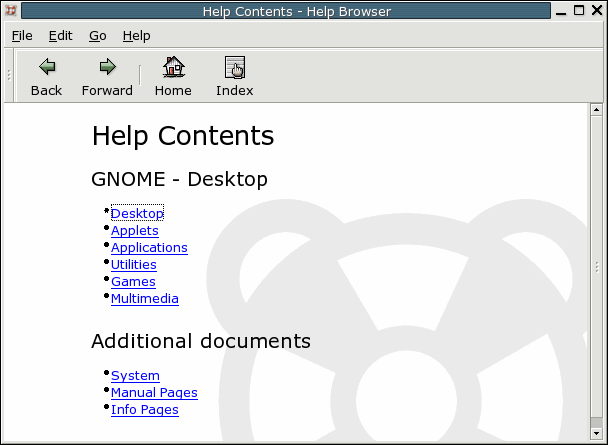
\includegraphics{yelp01.eps}~~~~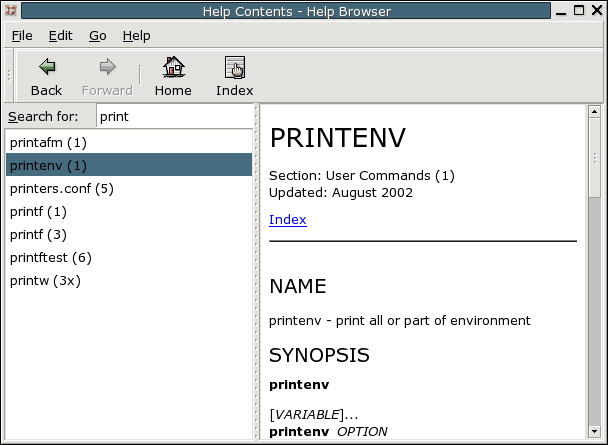
\includegraphics{yelp02.eps}}\caption{GNOME Help browser}\label{fig:yelp}}}%
{\leftskip=\moveback\parbox{\headwidth}{\center\scalebox{.35}{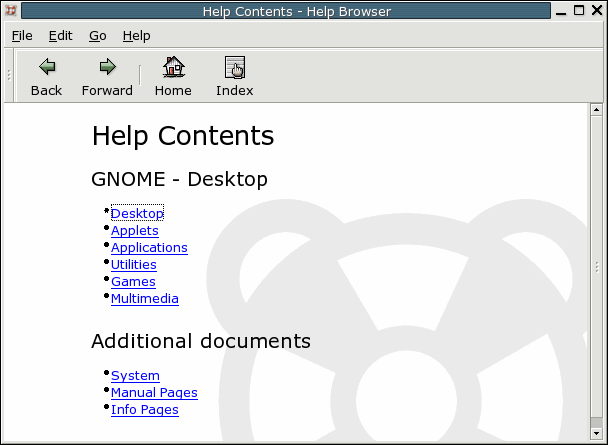
\includegraphics{yelp01.eps}~~~~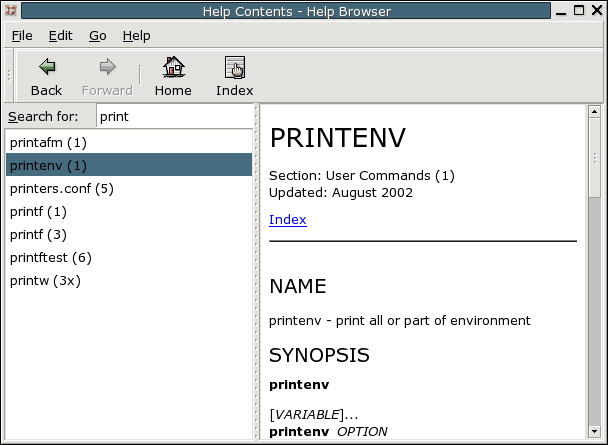
\includegraphics{yelp02.eps}}\caption{GNOME Help browser}\label{fig:yelp}}}
\end{figure}

\begin{figure}[t]
\ifthenelse{\isodd{\pageref{fig:khelpcenter}}}%
{\parbox{\headwidth}{\center\scalebox{.32}{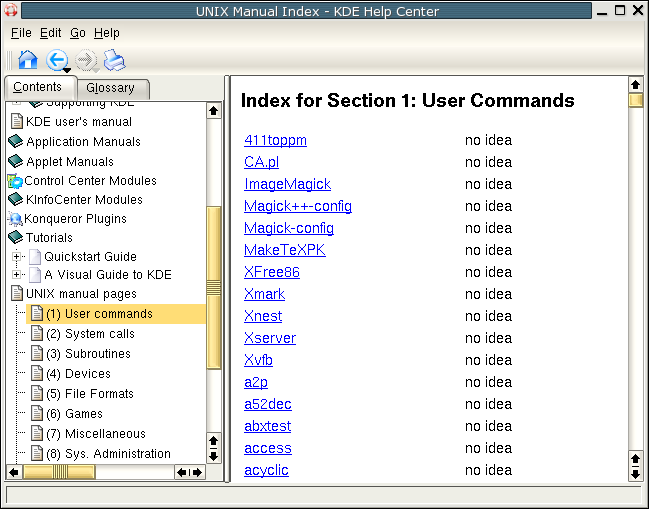
\includegraphics{khelpcenter01.eps}~~~~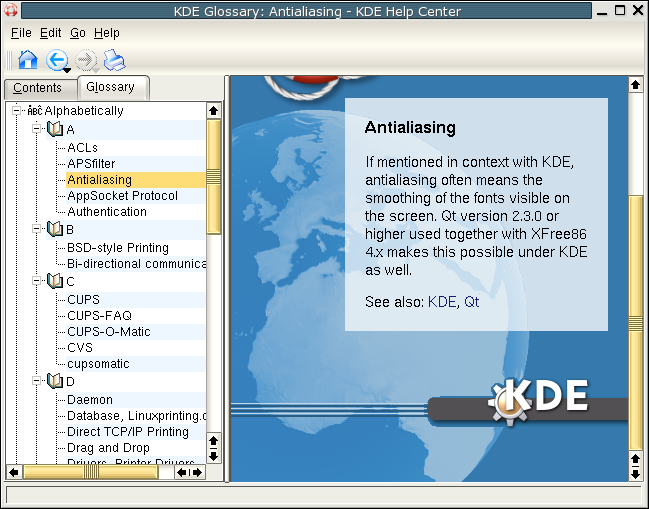
\includegraphics{khelpcenter02.eps}}\caption{KDE Help center}\label{fig:khelpcenter}}}%
{\leftskip=\moveback\parbox{\headwidth}{\center\scalebox{.32}{\includegraphics{khelpcenter01.eps}~~~~\includegraphics{khelpcenter02.eps}}\caption{KDE Help center}\label{fig:khelpcenter}}}
\end{figure}


\subsubsection{Help �ͧ bash ����}
�ҡ��ǧ����ҹ��������������Ҥ���觷����������������շ�駤�������㹫�������Ѻ����зӡ���ͧ����Ф������¹͡������������¡���������ҹ. �����͡�����������㹢ͧ��������ö��ҹ����¤���� ``\cmd{man bash}'' ���� ``\cmd{info bash}''. �����͡���� \cmd{bash} �������Ҵ�, ����������è���ҹ�����͹��˹���ͺ.

�͡�ҡ����� \cmd{man} ���� \cmd{info} ����, bash �����դ���� \cmd{help}\cindex{help}\refcmd{help} �ʴ��Ը���������Ф�͸Ժ�����ҧ���������������ͤ�����������������. �����觤���� \cmd{help} ��������ʴ���ª��ͤ���觷������ö͸Ժ����.  ������ҧ��

\begin{MyExample}[����� \cmd{help} ͸Ժ�¤�������㹢ͧ����]
\begin{MyEx}
$ \cin{help cd}
cd: cd [-L|-P] [dir]
    Change the current directory to DIR.  The variable $HOME is the
    default DIR.  The variable CDPATH defines the search path for
    the directory containing DIR.  Alternative directory names in CDPATH
    are separated by a colon (:).  A null directory name is the same as
    the current directory, i.e. `.'.  If DIR begins with a slash (/),
    then CDPATH is not used.  If the directory is not found, and the
    shell option `cdable_vars' is set, then try the word as a variable
    name.  If that variable has a value, then cd to the value of that
    variable.  The -P option says to use the physical directory structure
    instead of following symbolic links; the -L option forces symbolic 
    links to be followed.
\end{MyEx}
\end{MyExample}

��Ҥ�͸Ժ������Թ˹��˹�Ҩ�, ����Ҩ���� \cmd{less}\mymemo{����ػ����� \cmd{less} ���˹�� \pageref{tab:lesskey}.} ����㹡���ʴ���.

\begin{MyExample}[����� \cmd{help} �����Ѻ \cmd{less}.]
\begin{MyEx}
$ \cin{help set | less}
\end{MyEx}
\end{MyExample}

\subsection{�͡��áӡѺ�������ҹ}
���ҵԴ����������ҧ�����͡��ù͡�˹�ͨҡ man page �Ҵ���. �͡�������ҹ���Ҩ�����͡����й������, ˹ѧ���͹حҵ�, ������������� ��� ������ \cmd{/usr/share/doc}. �ҧ�����Ҩ�����͡��á����ҹẺ HTML\myvocab{h}{HTML (Hyper Text Markup Language)}{�ҵðҹ����Ѻ��¹�͡��÷�������ҧ World Wide Web. �ٻẺ�ͧ������������硫�����������ҹ����������. ������¹�ӡѺ��ǹ�������Ǣ��, ������, �ٻ�Ҿ ���. �»á�Ԩ�����纺������� (web browser) ����� HTML. ��纺�������з�˹�ҷ��Ѵ˹�Ҩ��Ҿ��������¹�ӡѺ�������.} ����á���չ������. ������͡���Ẻ HTML ����\emph{�������� (browser)} �� \cmd{mozilla}, \cmd{konqueror} �Դ��ҹ� X �Թ�����. ���Ͷ�ҵ�ͧ�����ҹ������Թ�š����������Ẻ�硫������� \cmd{lynx} ���� \cmd{w3m}.\mymemo{\cmd{w3m} ���� key binding ���Ẻ \cmd{vi} ��� \cmd{emacs} ��������. ������������֡����͹�Ѻ��ྨ���� \cmd{less} ���繺�������. ��ԧ����� \cmd{w3m} ����ö����ྨ���������.}

\subsection{�����ŷҧ�Թ������}
\subsubsection{���䫴����ҧ�繷ҧ��âͧ��ʷ�Ժ�Ǫѹ��ҧ�}
��ʷ�Ժ�Ǫѹ��鹹ӵ�ҧ��ѡ�������䫴�������͡��÷������ǡѺ��ʷ�Ժ�Ǫѹ�� �����͡�õԴ��� (Installation Guide), ���������������ҹ (User's Guide), ����������Ѻ�������к� (System Administrator's Manual) ���. �����ʹ�����ö价�����䫴�ͧ��ʷ�Ժ�Ǫѹ���������������͡��÷���ͧ���.

�͡�ҡ���䫴�ͧ��ʷ�Ժ�Ǫѹ�����ѧ�����䫴� The Linux Document Project (TLDP)\cite{tldp} ����Ǻ����͡��õ�ҧ������¡��� HOWTO, Guide, FAQ\myvocab{f}{FAQ (Frequently Asked Questions}{�������Ӷ����Фӵͺ������ѹ������ػ��������繢���������Ѻ����蹷���դӶ�����ǡѹ.} ���. �͡��÷�����������Ǻ����� TLDP �������鹡Ѻ��ʷ�Ժ�Ǫѹ�������¹��������Ѥ÷����š. �͡�����ѡ�������ѧ�������ա�����������������. �͡��� HOWTO ���͡��÷����Ш���������´���������ͧ�����仨��֧����ͧ੾�д�ҹ�� �Ըա�������������, ������ҧ VPN\myvocab{v}{VPN (Virtual Private Network)}{��������͢����Ҹ�ó����Թ������㹡���Ѻ�觢����������Ըա���ѡ�Ҥ�����ʹ��¢ͧ�����Ŵ���. �ٴ������͡�����ҧ���͢��·���դ�����ʹ����٧ (�蹡��ŧ����) �����͢����Ҹ�ó�.} ���. �͡����ա�������������ҹ�ͧ TLDP �ա�����������͡�����Ƿ����˹ѧ������¡��� Guide ��ҧ��� Advanced Bash-Scripting Guide, The Linux System Administrators' Guide �繵�. �͡�������ҹ����������¿�������� HTML, PDF, PostScript ���. 


���觢����ŷ���ջ���ª���ա����������䫴��ԡ���Ң������� Google, Yahoo ���. �ҡ������ջѭ�ҡ������������Դ error ��鹵͹��ҹ, ������ö�Ӣ�ͤ��� error ���令��Һ��Թ��������. �͡�ҡ���Ҩҡ���䫴�����, ����Ң����Ũҡ������ػ�蹨ҡ \url{http://groups.google.com} 㹺ҧ���駨�������ŷ����������纡���. 

���觢����������������Ҩ�ж���Ӷ��������纺���, ����� (forum), mailing list �繵�. ���䫴������·������ҹ����ö����ͺ�ѭ�ҵ�ҧ����ʴ����㹵��ҧ��� \ref{tab:forums}.

\myvocab{u}{URL (Uniform Resource Locator)}{�Ըա����ҧ�ԧ���觢��������͡��÷ҧ�Թ������. ������ҧ�� http://linux.thai.net:80/plone ��Сͺ������ǹ��ҧ����� ��ⵤ�� (http), �������� (linux.thai.net), �����Ţ���� (80) ��� path (plone).}
\begin{table}[!htb]
\caption{���䫴���ؤ�Ŷ���ͺ�ѭ����.}\label{tab:forums}
\bigskip
\begin{tabular}{l|p{.6\textwidth}}
\hline
\multicolumn{1}{c|}{���䫴�} & \multicolumn{1}{|c}{URL}\\
\hline
Thai Linux Working Group & \url{http://linux.thai.net}\\
Linux Siam & \url{http://www.linuxsiam.com}\\
Thai Linux Cafe & \url{http://thailinuxcafe.com}\\
Tux Crazy & \url{http://www.tuxcrazy.com}\\
Grandlinux Solution & \url{http://www.grandlinux.com}\\
\hline
\end{tabular}
\end{table}



\section{��û�Ѻ������}
�»á�������Թء���ʷ�Ժ�Ǫѹ�������ҹ�Դ��駹���ѡ�л�Ѻ���������������º��������. ��ҧ���駤�ҵ������Ҿ�Ǵ���������繵�ҧ�������, ��ҧ���Ѻ�觾�����������§�������, ��ҧ�����ҧ alias ������ ���. 㹪�ǧ�����Ҩ��Ҵ��Ըա�û�Ѻ�����������������ҹ�����дǡ���. ������¹�������ǡѺ�к�����֡�����觢��.

\subsection{����駤���������}
\mymemo{㹷����Ф�ͺ���������Ңͧ bash ��ҹ��.}�ҡ������ҧ������ҧ alias (˹�� \pageref{sec:alias}) ����ҹ��, alias ������ҧ��鹨������������ӧҹ������ҹ��. �����Ҩ������ҹ�������� alias ���������ҧ������觷����һ�Ѻ������������. ��к��ٹԡ��, �ѡ����\emph{����駤��������� (initialization file)}\gindex{initialization file}\mymemo{������ѧ���, ��ҧ�����¡����駤������������ init file, rc file\gindex{rc file} ���� dot file\gindex{dot file}. ����駤����������ѡ����������˹�Ҵ��¨ش (\cmd{.}) �����������觤���� \cmd{ls} �����ͧ������, �֧���¡��� dot file. �ҧ���ա�õ�駪������Ѵਹ�� \cmd{.bashrc} �¡����� ``rc''. �ҡ��ú͡���ҡѹ��, ``rc'' ����Ҩҡ run command. ����Ǥ�����������¹����觷���ͧ��÷����੾���������������������ӧҹ.} ������硫��������ҹ��, ������Ѻ��¹������������, ��Ѻ�觤�ҵ����, ��Ѻ�觾ĵԡ����ͧ�����. ������蹡ѹ������駤��������鹢ͧ�к� (system wide) �����ǹ�ؤ��.

�����������ҹ��������͵�駤��������鹢ͧ�к���鹨�ᵡ��ҧ�ѹ�������Ѻ�������ͧ���������������͡�Թ�������������ԧ��ͺ. 㹡óշ������͡�Թ����, �������ҹ���������鹨ҡ��� \cmd{/etc/profile} ���������駤��������鹢ͧ�к���͹. ��ѧ�ҡ��鹨е�Ǩ�����������á��������� \cmd{.bash\_profile} ���� \cmd{.bash\_login} ���� \cmd{.profile} ����������ӴѺ. ��������������˹�觷����������ǡ����ҹ�����Ҩҡ����������ԡ�����������. �������� \cmd{.bash\_logout} ������á����, �������ҹ�����͹�����ԡ��÷ӧҹ. 

㹡óշ���������ԧ��ͺ�� ����������� \cmd{xterm}\mymemo{��������������Թ�������������ҧ��Դ�� \cmd{gnome-terminal} ����ö���͡����Ҩ�����͡�Թ�������������ԧ��ͺ.} ����������鹨���ҹ�������������� \cmd{.bashrc} �������������á������ҹ��. 

\begin{figure}[!htb]
\plfigure{.8}{login_logout.eps}{����駤��������鹢ͧ \cmd{bash}}{login_logout}
\end{figure}

���ͧ�ҡ����������������ҧ�ѹ����ҹ����駤��������鹷��ᵡ��ҧ�ѹ仴���.
�ѧ��鹶�Ҩе�駤�����ͻ�Ѻ�������è����ѧ���������������ѧ����������ҹ����駤��������鹨ҡ����˹.
�Թء���ʷ�Ժ�Ǫѹ�ҧ���»�Ѻ������� \cmd{.bash\_profile} ���������ҹ���
\cmd{.bashrc} �ա��ʹ���. ���¤�����������Ҽ���������͡�Թ�������������ԧ��ͺ,
��û�Ѻ����������¹�������ж١��ҹ����. 

\subsection{��� \cmd{/etc/profile}}
��ѧ�ҡ����йӡ����������Ф���觵�ҧ�仾����������, ����ͧ�Ҵٵ�����ҧ����駤������������� \cmd{/etc/profile} �������Թء���ʷ�Ժ�Ǫѹ Gentoo �ѹ. �����Ңͧ������ᵡ��ҧ�ѹ�����ʷ�Ժ�Ǫѹ���µ�ҧ������˹�ҷ������͹�ѹ��ͻ�Ѻ�觤��������鹢ͧ��͡�Թ������к�. ��������������������������ͧ��¹�ͧ����������䢶������դ����������ǡѺ�������ҧ��§�������������ռš�з��Ѻ�ء����к�. ��ҵ�ͧ��û�Ѻ�觤�������������੾�кؤ���������� \cmd{\$HOME/.bash\_profile}.
\mymemo{����ͧ����\raisebox{8pt}{\wrap{}} ���ʴ���������ҷ����¹�ѧ����㹺�÷Ѵ���ǡѹ���鹺�÷Ѵ���������ҹ���¢����ҹ��.}

\begin{MyExample}[����駤��������鹢ͧ����]\label{ex:profile}
\begin{MyEx}
$ \cin{cat -n /etc/profile}
     1  # /etc/profile:
     2  # $Header: /home/cvsroot/gentoo-src/rc-scripts/etc/profile,v\wrap
1.23 2003/04/29 21:23:18 azarah Exp $ 
     3
     4  if [ -e "/etc/profile.env" ]
     5  then
     6          . /etc/profile.env
     7  fi
     8
     9  # 077 would be more secure, but 022 is generally quite realistic
    10  umask 022
    11
    12  if [ `/usr/bin/whoami` = 'root' ]
    13  then
    14          # Do not set PS1 for dumb terminals
    15          if [ "$TERM" != 'dumb'  ] && [ -n "$BASH" ]
    16          then
    17                  export PS1='\bs{}[\bs{}033[01;31m\bs{}]\bs{}h \bs{}[\bs{}033[01;34m\bs{}]\bs{}W \wrap
\bs{}$ \bs{}[\bs{}033[00m\bs{}]'
    18          fi
    19          export PATH="/bin:/sbin:/usr/bin:/usr/sbin:${ROOTPATH}"
    20  else
    21          # Do not set PS1 for dumb terminals
    22          if [ "$TERM" != 'dumb'  ] && [ -n "$BASH" ]
    23          then
    24                  export PS1='\bs{}[\bs{}033[01;32m\bs{}]\bs{}u@\bs{}h \bs{}[\bs{}033[01;34m\bs{}]\wrap
\bs{}W \bs{}$ \bs{}[\bs{}033[00m\bs{}]'
    25          fi
    26          export PATH="/bin:/usr/bin:${PATH}"
    27  fi
    28  unset ROOTPATH
    29
    30  if [ -z "$INPUTRC" -a ! -f "$HOME/.inputrc" ]
    31  then
    32          export INPUTRC="/etc/inputrc"
    33  fi
    34
    35  # Extract the value of EDITOR
    36  [ -z "$EDITOR" ] && EDITOR="`. /etc/rc.conf 2>/dev/null; \wrap
echo $EDITOR`"
    37  [ -z "$EDITOR" ] && EDITOR="`. /etc/conf.d/basic 2>/dev/null; \wrap
echo $EDITOR`"
    38  [ -z "$EDITOR" ] && EDITOR="/bin/nano"
    39  export EDITOR
\end{MyEx}
\end{MyExample}
%$

\subsubsection{��������}
��÷Ѵ��� 1 ��� 2 ��鹵鹺�÷Ѵ��������ͧ���� number (\cmd{\#}) ������������Ť�����觷����¹��ѧ����ͧ���� number ���ش��÷Ѵ. �ͧ��÷Ѵ�á������¡���\emph{�������� (comment)}\mymemo{����� comment ���������µç������ ``�����˵�''. ��㹷�������Ѻ�Ѿ����Ҥ�������.} ����¹͸Ժ�������ҷ������������. 

\subsubsection{��Ǩ�ͺ������ \cmd{if}}
��÷Ѵ��� 4 �֧ 7 �繡�õ�Ǩ�ͺ�������� \cmd{/etc/profile.env} ���������¤���� \cmd{if}.\cindex{if}\myexplanation{if}{�繤���觼���������������͵�Ǩ�ͺ�óյ�ҧ�.}
\begin{MyVerbatim}
if \textit{COMMAND}\mycomment{���ʶҹС�è�������� 0 �ж������繨�ԧ}
then
    \textit{COMMAND}\mycomment{����觷����㹡óշ���繨�ԧ}
    ...
elif \textit{COMMAND}\mycomment{��Ǩ�ͺ���� if �ա����}
then
    \textit{COMMAND}
    ...
else
    \textit{COMMAND}\mycomment{����觷����㹡ó����� (��)}
    ...
fi\mycomment{����õ�Ǩ�ͺ���� if}
\end{MyVerbatim}
����ѧࡵ�����觷��������ѧ����� \cmd{if} �繤������Ф���觹��ж١��зӡ�è�ԧ. ��Ҥ���觨���Ժ�ó�������բ�ͼԴ��Ҵ (ʶҹС�è��� 0) ��ж����ҡ�õ�Ǩ�ͺ�繨�ԧ. �С�зӡ�ä���觷������㹪�ǧ \cmd{then} ����. ��÷Ѵ��� 4 ����觷����㹡�õ�Ǩ�ͺ��ͤ���� \cmd{[}\cindex{[} ����繤���������������͹�Ѻ����� \cmd{test} (˹�� \pageref{cmd:test}). ����� \cmd{[} ��ͧ�����������������ش������ \cmd{]} ���������������º��������͹�Ѻ��¡ó�ͧ�����. ����Ǥ�� ``\cmd{[ -e \dq/etc/profile.env\dq ]}''\mymemo{����ѧࡵ�����ѧ \cmd{[} ��С�͹˹�� \cmd{]} ��ͧ�ժ�ͧ����� \cmd{[} �繤������� \cmd{]} �������������ͧ�����.} ��¹���աẺ��� ``\cmd{test -e \dq/etc/profile.env\dq}''. 

\subsubsection{��ҹ����������������������}
�������� \cmd{/etc/profile.env}\mymemo{���� \cmd{/etc/profile.env} �ա�û�С�Ȥ�ҵ������Ҿ�Ǵ������ҧ��� Gentoo ��駤�����.} �������������ҹ�����Ҥ���觷������������. ����ͧ���¨ش (\cmd{.}) 㹺�÷Ѵ��� 6 ���繤��������������ҧ˹�觷�˹�ҷ����ҹ����觷�������������������������. ����������� \cmd{.} �Ѻ�����������������������͹�Ѻ��ùӤ���觷����¹�����������ҡ�зӡ���������������. ����� \cmd{.}\cindex{.} �ټ��༹���������͹�Ѻ�繤����, �֧�դ���觷����ҹ�������㨤�� \cmd{source}\cindex{source} ����繤���觷���˹�ҷ������͹�Ѻ \cmd{.} �ء��С��.\refcmd{source}

\bigskip
��÷Ѵ��� 10 �繡�õ�駤���Է�������������������������� \cmd{umask}. ��͸Ժ�¤���觹��㹪�ǧ����й�����ͧ�Է����������. 

\subsubsection{��駤�Ҿ�����}
\begin{table}[!htbp]
\center
\caption{escape sequence �����Ѻ���������}\label{tab:shellprompt}
\bigskip
\begin{tabular}{l|p{.7\textwidth}}
\hline
\multicolumn{1}{c|}{escape sequence} & \multicolumn{1}{|c}{��������}\\
\hline
\cmd{\bs{}a} & �ѡ��� ASCII ��д��. ������ʴ����ú�˹�Ҩ���������§��д���͡�ҧ��⾧.\\
\cmd{\bs{}d} & �ʴ��ѹ���㹾�������ٻ�ͧ ``�ѹ ��͹ �ѹ���''.\\
\cmd{\bs{}D\{\textit{FORMAT}\}} &  �ʴ��ѹ�����ٻẺ����кش��� \cmdit{FORMAT}. \cmd{strftime(3)} �����������ǡѺ \cmdit{FORMAT}.\\
\cmd{\bs{}e} & �ѡ��� ESC.\\
\cmd{\bs{}h} & ������ʫ�觨��ʴ�������ʶ֧����ͧ���¨ش (\cmd{.}) ����͵���á��ҹ��. �蹶�Ҫ�������� \cmd{localhost.localdomain}, \cmd{\bs{}h} ����� \cmd{localhost}.\\
\cmd{\bs{}H} & �������.\\
\cmd{\bs{}j} & �ӹǹ��ͺ���Ǻ�����������.\\
\cmd{\bs{}l} & basename �ͧ�����������Թ�ŷ����. �������Թ�ŷ�����ʹ������� \cmd{/dev/pst/6}, \cmd{\bs{}l} ���� \cmd{6}.\\
\cmd{\bs{}n} & �ѡ��� newline ��鹺�÷Ѵ����.\\
\cmd{\bs{}r} & �ѡ��� cariiage return ��鹺�÷Ѵ����.\\
\cmd{\bs{}s} & ������������.\\
\cmd{\bs{}t} & ���һѨ�غѹẺ 24 ��������� \cmd{23:59:59}.\\
\cmd{\bs{}T} & ���һѨ�غѹẺ 12 ��������� \cmd{11:59:59}.\\
\cmd{\bs{}@} & ���һѨ�غѹẺ 12 ��������� \cmd{11:59 PM}.\\
\cmd{\bs{}A} & ���һѨ�غѹẺ 24 ��������� \cmd{23:59}.\\
\cmd{\bs{}u} & ���ͼ����.\\
\cmd{\bs{}v} & �����ѹ�ͧ bash ���������� \cmd{2.00}.\\
\cmd{\bs{}V} & ����ʢͧ bash ���������� \cmd{2.00.0} (�����ѹ + patch level).\\
\cmd{\bs{}w} & ��á���շ��ӧҹ������ \cmd{\~} (�����á����).\\
\cmd{\bs{}W} & ��á���շ��ӧҹ������ \cmd{somchai} (�����á���բͧ somchai).\\
\cmd{\bs{}!} & �����Ţ����ѵԤ���觢ͧ����觹��.\\
\cmd{\bs{}\#} & �����Ţ (�ӹǹ) �����.\\
\cmd{\bs{}\$} & �ʴ������� \cmd{\#} ����� root ���� \cmd{\$} ����.\\
\cmd{\bs{}\textit{nnn}} & �Ţ�ҹỴ \cmdit{nnn} ����¹᷹�ѡ��з���������þ������.\\
\cmd{\bs\bs} & backslash (\cmd{\bs})\\
\cmd{\bs{}[} & ������ѡ��з���ʴ��ҧ˹�Ҩ�����������;�����ѡ��ФǺ��������Թ��.\\
\cmd{\bs{}]} & ���ѡ��з���ʴ��ҧ˹�Ҩ������.\\
\hline
\end{tabular}
\end{table}
��÷Ѵ��� 12 �֧ 27 �繡�õ�駤�Ҿ�������� \cmd{PATH}. ���ա�õ�Ǩ�ͺ��Ҷ�Ҽ������ root ��е�駤�Ҿ�������� \cmd{PATH} ����ҧ�ҡ���������. �ç����ա���� \cmd{test}\refcmd{test} ��Ǩ�ͺ�Ţͧ����� \cmd{whoami}\cindex{whoami}\refcmd{whoami} �������� root �������. ��͹���е�駤�Ҿ������ա�õ�Ǩ�ͺ��Դ�ͧ�����Թ����������\emph{�����Թ��Ẻ dumb (dumb terminal)}.\myvocab{d}{dump terminal}{�������Թ����ҳ����á�. ����դ�������ö㹡�èѴ��˹�Ҩ�, ������� (��Ǵ�) �����բմ�ӡѴ����. ����Ǥ���������Թ��Ẻ�����, ����§�س���ѵ����ͧ�鹷��ͨ���ҹ����ҹ��.} 

��Ңͧ������������㹵������Ҿ�Ǵ���� \cmd{PS1}\gindex{ps1@\cmd{PS1}} �٫Ѻ��͹�������ԧ����ҡ���зӤ�������. ���������駹���繾����������ի����س���ѵԢͧ
\emph{�����Թ���ҵðҹ ANSI (ANSI terminal)}\gindex{ansi termial@ANSI terminal} 㹡�õ����յ�ҧ�. ��Ңͧ������㹺�÷Ѵ��� 17 ��� 24 ���͡���� 3 ��ǹ����.


\begin{enumerate}
\item escape sequence �ͧ����\\
escape �ͧ����й�˹�Ҵ�������ͧ���� backslash (\cmd{\bs}). �ҡ������ҧ��� \cmd{/etc/profile} ��÷Ѵ��� 17 ���� \cmd{\bs{}[}, \cmd{\bs{}]}, \cmd{\bs{}h}, \cmd{\bs{}W} ��� \cmd{\bs{}@}. ���ҧ��� \ref{tab:shellprompt} �ʴ� escape sequence ���������Ф�͸Ժ��.
\item ANSI escape sequence\\
\emph{ANSI escape sequence}\gindex{ansi escape sequence@ANSI!escape sequence} �� escape sequence �����Ǻ��������Թ�ŷ���դس���ѵԵ����� ANSI ��˹�. �����Թ������������������ X �Թ����·���仡�Ѵ����㹾ǡ���. �ҡ��÷Ѵ��� 17, ��ǧ����� ANSI escape sequence ��� ``\cmd{\bs{}033[01;31m}''.
\item �ѡ��з����\\
�ѡ��з���令������ͧ���������ѡ�÷���ͧ�����ҧ�����Թ������դ������¾��������Ѻ����. �ҡ��÷Ѵ��� 17 �����ͧ�. �ҡ��÷Ѵ��� 24 ��������ͧ���� \cmd{@}.
\end{enumerate}

\subsubsection{��駤�ҵ������Ҿ�Ǵ����}
������÷Ѵ��� 28 ��������繡�õ�駤�ҵ������Ҿ�Ǵ������ҧ�. ��÷Ѵ��� 28 ��ź�������Ҿ�Ǵ���� \cmd{ROOTPATH} ��觶١��駤�Ҩҡ�����ҹ��� \cmd{/etc/profile.env} ��÷Ѵ��� 6 ���¤���� \cmd{unset}.\cindex{unset}\refcmd{unset} 

��÷Ѵ��� 30 �֧ 33 �繵�駤�ҵ������Ҿ�Ǵ���� \cmd{INPUTRC} ����ա�õ�Ǩ��͹��Ҷ�ҵ���� \cmd{INPUTRC} ���դ�������� 0\mymemo{������դ�������� 0 ���¶֧����դ�����͵��������յ�ǵ�.} (\cmd{-z \$INPUTRC})\refcmd{test} ��� (\cmd{-a}) �������� \cmd{\$HOME/.inputrc} (\cmd{! -f \$HOME/.inputrc}) �֧�е�駤�ҵ������Ҿ�Ǵ���� \cmd{INPUTRC} �� \cmd{/etc/inputrc}. �������Ҿ�Ǵ���� \cmd{INPUTRC} �繵���÷���纪��������������駤��������鹢ͧ\emph{�ź���� readline (readline library)}.\gindex{readline} �ź���չ����� bash ��������Ѻ����㹡����䢺�÷Ѵ�����, ��������������. ����駤����������»����¨������ \cmd{.inputrc} �������������á���բͧ�����ѧ��鹨֧�ա�õ�Ǩ�ͺ���������������������. �������յ���к���е�駤�������������к���������. 

��÷Ѵ��� 36 ��������繡�õ�駤�ҵ������Ҿ�Ǵ���� \cmd{EDITOR}. ����� \cmd{EDITOR} �������������������ҹ�����ͧ��������������������������������óҸԡó�֧�������ö��������. �ó�����������鹨����¡��óҸԡó����к�����㹵������Ҿ�Ǵ���� \cmd{EDITOR} ���������������������ͧ���. ������������ҧ����� \cmd{less} (����͵�ͧ�������������), \cmd{cvs} (����͵�ͧ���������������¹�����˵�) ���. 


\subsection{�շ����������Թ��Ẻ ANSI}
ANSI escape sequence �� escape sequence �����Ǻ������ͻ�Ѻ��ĵԡ����ͧ�����Թ�ŷ�����ҵðҹẺ ANSI. escape sequence �������ǡѺ��û�Ѻ�������ٻẺ��
\begin{MyVerbatim}
<ESC>[{\textit{attr1}};...;{\textit{attrn}}m
\end{MyVerbatim}
\begin{itemize}
\item \cmd{<ESC>} ����ѡ��� ESC. ���ͧ�ҡ�ѡ��� ESC �������ö�ʴ���������Թ��������� \cmd{\bs{}033} ����繤�Ңͧ�ѡ��� (�Ţ�ҹỴ) ᷹㹺�÷Ѵ�����.

\item \cmd{[} �繡��������鹤س�ѡɳТͧ�ѡ�÷���ͧ����ʴ�.
\item ����Ţ���Ѵ�ҡ \cmd{[} ��ͤ�ҷ���к��� 01 ���¶֧����˹�. 33 ���¶֧�����ѡ��������ͧ. 㹡���кؤ���ҡ�����ͧ���ҧ���������ͧ���� semi-colon (\cmd{;}) ���.
\item \cmd{m} �繡����觵�駤�ҷ���к�.
\end{itemize}
\mymemo{�� Magenta ����շ���Դ�ҡ��ü�������, ��ᴧ (Red) ����տ�� (Blue). �� Cyan ����շ���Դ�ҡ��ü�������, ������ (Green) ����տ�� (Blue).}%

\begin{table}[!htb]
\center
\caption{ANSI escape sequence �������ǡѺ��. \cite{ansicolor}}\label{tab:ansiterminal}
\bigskip
\begin{tabular}{l|l}
\hline
\multicolumn{1}{c|}{���} & \multicolumn{1}{|c}{��͸Ժ��}\\
\hline
0 &	¡��ԡ��ҷ������������\\
1 &	���ѡ�÷���ʴ����������\\
2 &	���ѡ�÷���ʴ����ҧŧ\\
4 &	�մ�����\\
5 &	�ӵ���ѡ������оԺ\\
7 &	��Ѻ����¹�թҡ��ѧ�Ѻ�յ���ѡ��\\
8 &	��͹�ѡ�÷���ʴ�\\
30 &	���յ���ѡ���մ� (Black)\\	      
31 &	���յ���ѡ����ᴧ (Red)\\	      
32 &	���յ���ѡ�������� (Green)\\      
33 &	���յ���ѡ��������ͧ (Yellow)\\    
34 &	���յ���ѡ���տ�� (Blue)\\	      
35 &	���յ���ѡ����ᴧ��ǧ (Magenta)\\  
36 &	���� Cyan\\		      
37 &	���յ���ѡ���բ�� (White)\\       
40 &	��ҡ��ѧ�յ���ѡ���մ� (Black)\\	   
41 &	��ҡ��ѧ�յ���ѡ����ᴧ (Red)\\	   
42 &	��ҡ��ѧ�յ���ѡ�������� (Green)\\     
43 &	��ҡ��ѧ�յ���ѡ��������ͧ (Yellow)\\   
44 &	��ҡ��ѧ�յ���ѡ���տ�� (Blue)\\	   
45 &	��ҡ��ѧ�յ���ѡ����ᴧ��ǧ (Magenta)\\ 
46 &	��ҡ��ѧ�� Cyan\\		   
47 &	��ҡ��ѧ�յ���ѡ���բ�� (White)\\      
\hline
\end{tabular}
\end{table}


��õ�駤س�ѡɳо���ɢͧ��觷���ʴ��������Թ�Ţ������Ѻ��������ö�ͧ�����Թ�Ũ֧�ա�õ�Ǩ�ͺ�������ͧ�����Թ�š�͹��駤�ҹ��. ����Ҩ�з��ͧ�� \cmd{echo} ����� ANSI escape sequence �ٷҧ�����Թ�Ŵ��µ�����͡ \cmd{-e}.\refcmd{echo}

\begin{MyExample}[����� \cmd{echo} ����� ANSI escape sequence.]
\begin{MyEx}
\cin{echo -e "\bs{}033[1;4mBold and Underline\bs{}033[0m Normal \bs{}033[1mBold again"}
\underline{\bf{}Bold and Underline} Normal {\bf{}Bold again}
\end{MyEx}
\end{MyExample}

\subsection{���������}
�������������ѹ������յ����Ẻ�����ش�������������ͧ���´������ \cmd{\$} ���֧�����ʤ�Ի����п͹�����ɪ��� \cite{prompthowto}. ����������� bash ������ 4 ��Դ�纤�����㹵������Ҿ�Ǵ������ҧ�ѹ����
\begin{enumerate}
\item \cmd{PS1}\gindex{ps1@\cmd{PS1}}\\
�纤�Ҿ�������ѡ��������͡�Թ�������������ԧ��ͺ. ��ҨФ���¡Ѻ�������������繾�����������Ƿ���ش. ��С�û�Ѻ�觾�������ѡ�л�Ѻ�觤�� \cmd{PS1}. ����»����¢ͧ \cmd{PS1} ��� ``\cmd{\bs{}s-\bs{}v\bs{}\$ }''.\mymemo{��ѧ����ͧ���� \cmd{\$} �ժ�ͧ�˹�觵��.}
\begin{MyExample}[��һ����¢ͧ��������ѡ \cmd{PS1}.]
\begin{MyEx}
-bash-2.05b$ \cin{echo $PS1}
\bs{}s-\bs{}v$
\end{MyEx}
\end{MyExample}%$
�»á�����Ǵ�ʷ�Ժ�Ǫѹ�л�Ѻ�觤�� \cmd{PS1} ���������� \cmd{/etc/profile}.
\item \cmd{PS2}\gindex{ps2@\cmd{PS2}}\\
�纤�Ҿ������ͧ���ʴ��繾������������觤������診����˹�觺�÷Ѵ���Ǣ�鹺�÷Ѵ����. ����»����¢ͧ�������ͧ����� ``\cmd{> }''.
\begin{MyExample}[��һ����¢ͧ�������ͧ \cmd{PS2}.]
\begin{MyEx}
-bash-2.05b$ \cin{"Primary prompt $PS1}
> \cin{Secondary prompt $PS2"}
Primary prompt \bs{}s-\bs{}v$
Secondary prompt >
\end{MyEx}
\end{MyExample}%$
\item \cmd{PS3}\gindex{ps3@\cmd{PS3}}\\
�繾���������Ѻ����� \cmd{select}.\cindex{select}\refcmd{select} ����� \cmd{select} �繤����Ẻ��¡ó�ͧ���������ʴ�������͡�繢���������͡�ͺ�Ӷ��. 
\begin{MyExample}[�� \cmd{select} ����Ӷ��.]
\begin{MyEx}
$ \cin{echo What is your favorite character in One Piece?;\bs{}}
> \cin{select name in Luffy Nami Zoro Sanji Usopp Choper Robin;}
> \cin{do echo I like $name also!}
> \cin{break}
> \cin{done}
What is your favorite character in One Piece?
1) Luffy
2) Nami
3) Zoro
4) Sanji
5) Usopp
6) Choper
7) Robin
#? \cin{6}
I like Choper also!
$ \cin{echo $name}
Chopper
\end{MyEx}
\end{MyExample} 
��ҵ�駤�� \cmd{PS3}, ����� \cmd{select} ������ҷ��������繾�����᷹ ``\cmd{\#?}''.
\item \cmd{PS4}\gindex{ps4@\cmd{PS4}}\\
�繾��������ʴ�������ա�õԴ��� (trace) �����. ��õԴ�������觹������µ�駤�� \cmd{xtrace} �����ѹ������µ�����͡ \cmd{-x}. ��һ����¢ͧ \cmd{PS4} ��� \cmd{+}.
\begin{MyExample}[��õԴ�������������]\label{ex:shelltrace}
\begin{MyEx}
$ \cin{set -o xtrace} \mycomment{���� set -x}
++ echo -ne '\bs{}033]0;somchai@toybox:~\bs{}007'
$ \cin{echo Hello}
+ echo Hello
Hello
++ echo -ne '\bs{}033]0;somchai@toybox:~\bs{}007'
$ \cursorprompt
\end{MyEx}
\end{MyExample}%$
��õԴ��������������ջ���ª�����ҧ���������� debug ����ʤ�Ի��١����觤���觵�ҧ��ʤ�Ի��.
\end{enumerate}

��ѧ�ҡ��������ѡ�Ѻ�������������ҧ���������ͧ�Ҵٵ�����ҧ��õ�駤�Ҿ�����ҡ��觷�����¹��������. 
\begin{MyExample}[��û�Ѻ��Ҿ�����ҡ��觷�����¹��.]
\begin{MyEx}
$ \cin{export PS1="-\bs{}[\bs{}033[32m\bs{}d, \bs{}t\bs{}033[0m\bs{}]- [\bs{}w]\bs{}n\bs{}u@\bs{}h \bs{}$  "}
-\textcolor{green}{Tue May 18, 01:38:54}- [~]
somchai@toybox $ \cin{cd /usr/src/linux/Documentation/filesystems}
-\textcolor{green}{Tue May 18, 01:39:04}- [/usr/src/linux/Documentation/filesystems]
somchai@toybox $ \cursorprompt
\end{MyEx}
\end{MyExample}
�ҡ������ҧ�繡�����ҧ������������ͧ��÷Ѵ. ��÷Ѵ�á�͡���������á���շ��ӧҹ���� (full path). ��ǹ��÷Ѵ����ͧ�繾���������Һ͡���ͼ������Ъ������. ����Ѻ�����ʹ�����ͧ��õ�駤�Ҿ������������´, ����ö��ҹ��ҡ�͡��� Bash Prompt HOWTO \cite{prompthowto}.


\subsection{�ź���� readline}
���������й�仢�ҧ����������������ź���� readline ����㹡�û�Ѻ�觺�÷Ѵ�������ШѴ��û���ѵԤ����. ���ͧ�ҡ readline ���ź����, ������������ա����ͺ�Ѻ�����Ẻ CLI ������ö���ź���� readline �����. ������ҧ������� \cmd{gnuplot}\mymemo{\cmd{gnuplot} ���������¹��ҿ.} ������Թ������Ẻ CLI ������ö�� key binding ����͹�Ѻ�����Ѻ bash ���� �� \cmd{C-p} ��觤���觷���������� �繵�.

�ź���� readline ����ҹ������к��µ������Ҿ�Ǵ���� \cmd{INPUTRC} ���Ͷ������ա�õ�駤�ҵ���ù������ҹ���������鹨ҡ��� \cmd{\$HOME/.inputrc}\gindex{.inputrc@\cmd{.inputrc}}. ����ͧ�Ҵ������Ңͧ����駤��������鹢ͧ�ź���� readline �ѹ. 
\begin{MyExample}[����駤��������鹢ͧ�ź���� readline.]\label{ex:inputrc}
\begin{MyEx}
$ \cin{cat -n ~/.inputrc}
     1  $include /etc/inputrc
     2
     3  # be quiet
     4  set bell-style none
     5  set meta-flag on
     6  set input-meta on
     7  set convert-meta off
     8  set output-meta on
     9
    10  "\bs{}C-x\bs{}C-r": re-read-init-file			       
    11  "\bs{}M-m": "LANG=ja_JP XMODIFIERS='@xim=kinput2' mozilla &"   
    12  								       
    13	$if gnuplot						       
    14  "\bs{}M-m": "plot sin(x)\bs{}r"				       
    15  $endif                                                         
    16  "\bs{}M-xf": dump-functions
    17  "\bs{}M-xv": dump-variables
    18  "\bs{}M-xm": dump-macros
\end{MyEx}
\end{MyExample}

��͹����͸Ժ��������������, ��Ҿͨ��ѧࡵ�����Ҥ�������ͧ�����������ͧ���� number (\cmd{\#}) �����¡ó��������������͡�� 3 ��Դ�˭����
\begin{enumerate}
\item ��駤�ҵ����\\
��õ�駤�ҵ�������� \cmd{\~{ }/.inputrc} ����¡ó���
\begin{MyVerbatim}
set \textit{variable-name} \textit{value}
\end{MyVerbatim}
``\cmd{set \textit{variable-name} \textit{value}}'' 㹷�����������������������¡ó�ͧ����駤��������� readline, �й��������������. ���͵���÷���Ӥѭ��Ф���»����·�������� \cmd{\~{ }/.inputrc} ����.

\begin{itemize}
\item \cmd{bell-style} (\cmd{audible})\mymemo{��ҷ�������ǧ��纤�ͤ���»�����.}\\
�ٻẺ�ͧ��д�觷����������Թ��. \cmd{audible} ��������§��д���͡�ҧ��⾧. ������� \cmd{visible} ����������§��˹�ҨͨС�оԺ᷹. ��ǹ \cmd{none} �������������Դ���.
\item \cmd{completion-ignore-case} (\cmd{off})\\
��ҵ�駤���� \cmd{on} ����������������ͪ�������·������¡����ѡ�õ���˭�����ѡ�õ�����.
\item \cmd{completion-query-items} (\cmd{100})\\
�ӹǹ����繢մ������������Ҩ��ʴ���ǹ�������������㹡óշ����ǹ�������Թ�ӹǹ��������.
\item \cmd{convert-meta} (\cmd{on})\\
����դ���� \cmd{on}, readline ���ŧ�ѡ��з���� 8 �Ե�� 7 �Ե�ºԵ���Ỵ�����ѡ��� ESC �繵��᷹. �������Ѻ��������ö�ͧ�����Թ�Ŵ���.
\item \cmd{disable-completion} (\cmd{off})\\
��ҵ�駤���� \cmd{off} ������ա�����������.
\item \cmd{editing-mode} (\cmd{emacs})\\
��駤���Ըա�û�Ѻ�觺�÷Ѵ�����Ẻ \cmd{emacs} ���� \cmd{vi}.
\item \cmd{expand-tilde} (\cmd{off})\\
����ͧ���� tilde (\cmd{\~{ }}) ��᷹�����á����. ��ҵ�駤�ҵ���ù���� \cmd{on}, �����������С�Ш������ͧ���� tilde �� full path.
\item \cmd{input-meta} (\cmd{off})\\
��ҵ�駤���� \cmd{on}, readline ��͹حҵ��������������ѡ��� 8 �Ե. \cmd{meta-flag} �繵���÷����˹�ҷ������͹����õ�ǹ��.
\item \cmd{mark-directories} (\cmd{on})\\
��Ҥ���� \cmd{on}, �������������������������ͧ���� slash (\cmd{/}) ��ѧ������á���������¡��������ҧ������Ѵਹ.
\item \cmd{match-hidden-files} (\cmd{on})\\
readline ���ʴ����������ǹ������������������������鹵鹴��¨ش (\cmd{.}) ����. ��ҵ�駤���� \cmd{off} ��е�ͧ���������������鹵鹴��¨ش, ��ͧ�����ش��͹���� readline ��������������鹵鹴��¨ش���.
\item \cmd{output-meta} (\cmd{off})\\
��ҵ�駤���� \cmd{on}, readline ���ʴ��ѡ���Ẻ 8 �Ե����·��������������¹�� 7 �Ե. �������Ѻ�����Թ�ŷ�������.
\item \cmd{page-completions} (\cmd{on})\\
readline ����ྨ����Ẻ \cmd{more} 㹡���ʴ���ǹ������������ҡ���ҷ����ʴ���˹�Ҩ�������. ��ҵ�駤���� \cmd{off} �������ǹ�������ҡ�з������ҡ, ������١ú�ǹ����ྨ����. �Ҩ������� \kk{Shift}+\kk{PgUp} ������Ѻ仴���ǹ����������.
\end{itemize}
\item Key bindings\\
key binding ���������������� \cmd{C-p}, \cmd{C-k} ����ҹ���˹����ź���� readline ��駹��. �ź���� readline ��������������˹�������ͼ�����˹������ҡѺ����觢ͧ�ź���� readline. ��á�˹���Ҥ����˹��������������¡ó�ѧ���.
\begin{MyVerbatim}
\textit{keys}: \textit{action}
\end{MyVerbatim}

\cmdit{keys} �Ҩ���繪��ͤ����� readline ���˹������������ \cmd{DEL}, \cmd{ESC}, \cmd{ESCAPE} ���. ���ͤ�������ҹ������ö��ҹ��ҡ on-line manual ���� info �ͧ readline. \cmdit{keys} �աẺ��ͪش�������ͧ������ \kk{Ctrl} ��ҧ���ǵ�����¤������ (\cmd{\bs{}C-}), ����� \kk{Esc} ��͹���ǵ�����¤������ (\cmd{M-}), ���� ������ \kk{Esc} ��͹���ǵ�����¡�á����� \kk{Ctrl} ��ҧ������ǵ�����¤������ (\cmd{M-C-}). ��á���������ҹ�����Է�Ծ��Ҩҡ��óҸԡó� Emacs. 

\cmdit{action} �繡�á�зӷ���Դ�ҡ��á��������˹����. ��á�зӹ���Ҩ���繿ѧ�ѹ�ͧ readline ���������ҧ��÷Ѵ��� 10 �蹶�ҡ����� \cmd{C-x C-r} ����, ��á�зӤ�Ϳѧ�ѹ \cmd{re-read-init-file}. readline ����ҹ����駤��������鹷���˹��µ������Ҿ�Ǵ���� \cmd{INPUTRC} �ա����. �»á�Կѧ�ѹ����ҹ����� key binding �»�������������. ��ҵ�ͧ��������������͵�ͧ����к����Ѵਹ����¹ŧ�����駤�����������. 㹵��ҧ��� \ref{tab:readlinefunc}\mymemo{key binding �ҧ�����͸Ժ�������㹵��ҧ��� \ref{tab:controlterm} ��� \ref{tab:lineedit}} �ʴ� key binding �»�������Ъ��Ϳѧ�ѹ�������ѹ��ѹ.

\begin{table}[!htb]
\center
\caption{key binding �»�������пѧ�ѹ�ź���� readline �������ѹ��ѹ.}\label{tab:readlinefunc}
\bigskip\scriptsize
\begin{tabular}{|c|l||c|l|}
\hline
\multicolumn{2}{|c||}{key binding Ẻ \cmd{C-}} & \multicolumn{2}{|c|}{key binding Ẻ \cmd{M-}}\\
\hline
\cmd{C-@} &   \cmd{set-mark}&                                  \cmd{M-C-g} &   \cmd{abort}				       \\
\cmd{C-a} &   \cmd{beginning-of-line}&		                \cmd{M-C-h} &   \cmd{backward-kill-word}		       \\
\cmd{C-b} &   \cmd{backward-char}&		                \cmd{M-C-i} &   \cmd{tab-insert}			       \\
\cmd{C-d} &   \cmd{delete-char}&		                \cmd{M-C-j} &   \cmd{vi-editing-mode}			       \\
\cmd{C-e} &   \cmd{end-of-line}&		                \cmd{M-C-m} &   \cmd{vi-editing-mode}			       \\
\cmd{C-f} &   \cmd{forward-char}&		                \cmd{M-C-r} &   \cmd{revert-line}			       \\
\cmd{C-g} &   \cmd{abort}&			                \cmd{M-C-y} &   \cmd{yank-nth-arg}			       \\
\cmd{C-h} &   \cmd{backward-delete-char}&	                \cmd{M-C-[} &   \cmd{complete}				 \\      
\cmd{C-i} &   \cmd{complete}&			                \cmd{M-C-]} &   \cmd{character-search-backward}		   \\    
\cmd{C-j} &   \cmd{accept-line}&		                \cmd{M-space} &   \cmd{set-mark}			       \\
\cmd{C-k} &   \cmd{kill-line}&			                \cmd{M-\#} &   \cmd{insert-comment}			       \\
\cmd{C-l} &   \cmd{clear-screen}&		                \cmd{M-\&} &   \cmd{tilde-expand}			       \\
\cmd{C-m} &   \cmd{accept-line}&		                \cmd{M-*} &   \cmd{insert-completions}			 \\      
\cmd{C-n} &   \cmd{next-history}&		                \cmd{M--} &   \cmd{digit-argument}			       \\
\cmd{C-p} &   \cmd{previous-history}&		                \cmd{M-.} &   \cmd{yank-last-arg}			       \\
\cmd{C-q} &   \cmd{quoted-insert}&		                \cmd{M-<} &   \cmd{beginning-of-history}		       \\
\cmd{C-r} &   \cmd{reverse-search-history}&	                \cmd{M-=} &   \cmd{possible-completions}		       \\
\cmd{C-s} &   \cmd{forward-search-history}&	                \cmd{M->} &   \cmd{end-of-history}			       \\
\cmd{C-t} &   \cmd{transpose-chars}&		                \cmd{M-?} &   \cmd{possible-completions}		       \\
\cmd{C-u} &   \cmd{unix-line-discard}&		                \cmd{M-b} &   \cmd{backward-word}			       \\
\cmd{C-v} &   \cmd{quoted-insert}&		                \cmd{M-c} &   \cmd{capitalize-word}			       \\
\cmd{C-w} &   \cmd{unix-word-rubout}&		                \cmd{M-d} &   \cmd{kill-word}				       \\
\cmd{C-y} &   \cmd{yank}&			                \cmd{M-d} &   \cmd{forward-word}			       \\
\cmd{C-]} &   \cmd{character-search}&		                \cmd{M-l} &   \cmd{downcase-word}			       \\
\cmd{C-\_} &  \cmd{undo}&			                \cmd{M-n} &   \cmd{non-incremental-forward-search-history}     \\
\cmd{C-?} &       \cmd{backward-delete-char}&	                \cmd{M-p} &   \cmd{non-incremental-reverse-search-history}     \\
\cline{1-2}
\multicolumn{2}{c||}{}                  &                     \cmd{M-r} & \cmd{revert-line}\\
\multicolumn{2}{c||}{}			&	               \cmd{M-t} &  \cmd{transpose-words}			     \\
\multicolumn{2}{c||}{}			&			\cmd{M-u} & \cmd{upcase-word}				       \\
\multicolumn{2}{c||}{}			&                      \cmd{M-y} & \cmd{yank-pop}				 \\      
\multicolumn{2}{c||}{}			&			\cmd{M-\bs{}} & \cmd{delete-horizontal-space}		   \\    
\multicolumn{2}{c||}{}			&			 \cmd{M-\~}  &\cmd{tilde-expand}			     \\  
\multicolumn{2}{c||}{}			&			 \cmd{M-C-?} &  \cmd{backward-kill-word}		       \\
\multicolumn{2}{c||}{}			&			 \cmd{M-\_} &  \cmd{yank-last-arg}                             \\ 
\cline{3-4}
\end{tabular}	
\end{table}	

��÷Ѵ��� 16-18 �繡�á�˹� key binding ����Ѻ�ѧ�ѹ������� �ʴ���¡�âͧ key binding (\cmd{M-x f}) ��пѧ�ѹ����������� (\cmd{dump-functions}) �繵�. �ѧ�ѹ dump ����ҹ���»á������ա�õ�駤�� key binding ����»����¹͡�ҡ�е�駤���ͧ���������ҧ. ���������ö�ټŢͧ key binding �����ҡ������ҧ��� \ref{ex:dump-functions}.
\begin{MyExample}[�����ѧ�ѹ \cmd{dump-functions} �������˹�� \cmd{.inputrc}.]\label{ex:dump-functions}
\begin{MyEx}
$ \kk{Esc} \kk{x} \kk{f}
                                                              
abort can be found on "\bs{}C-g", "\bs{}C-x\bs{}C-g", "\bs{}M-\bs{}C-g".
accept-line can be found on "\bs{}C-j", "\bs{}C-m".
alias-expand-line is not bound to any keys
arrow-key-prefix is not bound to any keys
backward-byte is not bound to any keys
backward-char can be found on "\bs{}C-b", "\bs{}M-[D".
...
\end{MyEx}
\end{MyExample}%$


key binding �ѧ����ö�����¡\emph{���� (macro)}\myvocab{m}{macro}{\emph{����}. ���ͷ���˹������С�Ш�µ��令��������. ������ѹ���ҧ���ҧ��ҧ������ҫ�, \LaTeX{} ���.} ᷹�����ͻ���¤�����ҡ�˹��������������ҧ��� \ref{ex:inputrc} ��÷Ѵ��� 11. �����ͻ���¤�����ҡ�˹���ͧ��¹���������ͧ���� double quote (\dq). ���������ҧ��ҡ����� \cmd{M-m}, ����觷����¹�������������� ``\cmd{LANG=ja\_JP XMODIFIERS='@xim=kinput2' mozilla \&}'' ���á����㹺�÷Ѵ������������͹�����ҡ�鹾����.


\item ���͹�\\
��÷Ѵ����鹵鹴�������ͧ���´������ (\cmd{\$}) ����¡ó����к����͹����ͤ���觾����. ��÷Ѵ��� 1 �繡��������������鹨ҡ��� \cmd{/etc/inputrc} ���������. ��ǹ��÷Ѵ��� 13 �繡���к����͹��¡ key binding �������������. 㹵�����ҧ��������������� \cmd{gnuplot}, \cmd{M-m} ��᷹ ``\cmd{plot sin(x)\bs{}r}'' 㹺�÷Ѵ��������.

�͡�ҡ�����ҧ���͹䢵����������������, �ѧ����ö���ҧ���͹��觵�� mode (\cmd{emacs} ���� \cmd{vi}) ��л������ͧ�����Թ�������. �����ҹ��������´��������ҡ online manual ���� info �ͧ readline.
\end{enumerate}


\subsubsection{���������� readline �������?}
�����������Թ������Ẻ CLI �� \cmd{bash}, \cmd{wc}, \cmd{gnuplot} ��� �ѡ�����ź���� readline. �ѧ��鹨е�Ǩ�ͺ����������������ź���� readline ���������ͧ�� key binding �� \cmd{C-p}, \cmd{C-b} ��� �����դ�������ö��������������������. ��������ʴ�����������鹹�Ҩ����ź���� readline.

�Ըյ�Ǩ�ա�Ը�˹�觤�ʹ٨ҡ \emph{shared library}\mymemo{��ҧ�����¡ shared library ��� dynamic library.}\myvocab{s}{shared library}{���亹��շ������ǹ�ͧ�ź����. �����������ҧ����ͧ�����ǹ������ź��������㹵�������. ���¡�ա���ҧ˹����� dynamic library.} �������������. �»á��������������Թء���ѹ�������Ẻ dynamic, ����Ǥ�ͨ����¡�����������ͧ����ǹ������ź������������¡��. �Ըյ�Ǩ�ͺ������������� shared library ��������¤���� \cmd{ldd}.\cindex{ldd}\refcmd{ldd} ����� \cmd{ldd} �������������ʴ� shared library ����������.  
\begin{MyExample}[�� \cmd{ldd} ��Ǩ�ͺ shared library]
\begin{MyEx}
$ \cin{ldd /usr/bin/gnuplot}
        linux-gate.so.1 =>  (0xffffe000)
        lib3dkit.so.1 => /usr/lib/lib3dkit.so.1 (0x40015000)
        libvgagl.so.1 => /usr/lib/libvgagl.so.1 (0x4002a000)
        libplot.so.2 => /usr/lib/libplot.so.2 (0x40038000)
        libreadline.so.4 => /lib/libreadline.so.4 (0x4016b000)
	...
\end{MyEx}
\end{MyExample}%$
�������Ҽ��Ѿ��ͧ����� \cmd{ldd} �պ�÷Ѵ \cmd{libreadline} �������¤�����������������ź���� readline.

\subsection{��� \cmd{\$HOME/.bash\_profile}}\label{ex:bashprofile}
\begin{MyExample}[�����Ңͧ��� \cmd{.bash\_profile}]
\begin{MyEx}
     1  # /etc/skel/.bash_profile:
     2  # $Header: /home/cvsroot/gentoo-src/rc-scripts/etc/skel/.bash_profile,v\wrap
1.10 2002/11/18 19:39:22 azarah Exp $
     3
     4  #This file is sourced by bash when you log in interactively.
     5  [ -f ~/.bashrc ] && . ~/.bashrc
\end{MyEx}
\end{MyExample}

����駤��������鹢ͧ��͡�Թ�����ա���˹��������� \cmd{.bash\_profile}. 㹵�����ҧ \ref{ex:bashprofile} ����������ҧ������к��͹������ҧ�ѭ�ռ����. �������觷���ͧ��÷����͵�駤�Ҿ��������Ѻ��͡�Թ����੾�кؤ�š������¹������. 㹵�����ҧ����ա�û�Ѻ�������繾���ɹ͡�ҡ��ҹ����駤��������鹨ҡ��� \cmd{.bashrc} ��ҹ��. 

\subsection{��� \cmd{\$HOME/.bashrc}}
\begin{MyExample}[�����Ңͧ��� \cmd{.bashrc}]
\begin{MyEx}
     1  # /etc/skel/.bashrc:
     2  # $Header: /home/cvsroot/gentoo-src/rc-scripts/etc/skel/.bashrc,v \wrap
1.8 2003/02/28 15:45:35 azarah Exp $
     3
     4  # This file is sourced by all *interactive* bash shells on startup.  This
     5  # file *should generate no output* or it will break the scp and rcp commands.
     6
     7  # colors for ls, etc.
     8  eval `dircolors -b /etc/DIR_COLORS`
     9  alias d="ls --color"
    10  alias ls="ls --color=auto -F"
    11  alias ll="ls --color -l"
    12  
    13  alias rm='rm -i'
    14  alias cp='cp -i'
    15  alias mv='mv -i'
    16
    17  # Change the window title of X terminals
    18  case $TERM in
    19          xterm*|rxvt|Eterm|eterm)
    20                  PROMPT_COMMAND='echo -ne "\bs{}033]0;$\{USER\}@$\{HOSTNAME%%.*\}:\wrap
$\{PWD/$HOME/~\}\bs{}007"'
    21                  ;;
    22          screen)
    23                  PROMPT_COMMAND='echo -ne "\bs{}033_$\{USER\}@$\{HOSTNAME%%.*\}:\wrap
$\{PWD/$HOME/~\}\bs{}033\bs{}\bs{}"'
    24                  ;;
    25  esac
\end{MyEx}
\end{MyExample}%$
��� \cmd{.bashrc}\gindex{.bashrc@\cmd{.bashrc}} �����繵�����ҧ���������Ҩҡ�Թء�� Gentoo �蹡ѹ. ������������駤��������������ԧ��ͺ. ������ͧ�ҡ���� \cmd{.bash\_profile} �ա���к������ҹ��������仴���, ���Щй�鹤�ҷ�����·���Ѻ����������ռšѺ������͡�Թ����. ��û�Ѻ������������ѡ���繡�õ�駤�ҵ������Ҿ�Ǵ������й��ὧ, �������觤���觷�������Դ�������ʴ��͡�ҧ˹�Ҩ�. ���蹹�鹨з���� \cmd{scp} ��� \cmd{rcp}\mymemo{\cmd{scp} ��� \cmd{rcp} ���������ͻ�������ҹ�ҧ�������.} ���ӧҹ. 

��÷Ѵ��� 8 ���������� \cmd{ls} ����㹡���ʴ����������á����. ����� \cmd{dircolors}\cindex{dircolors}\refcmd{dircolors} ��Ѻ���շ�����Ѻ����� \cmd{ls}. ����� \cmd{dircolors} ���ʴ������ҡ�õ�駤�ҵ������Ҿ�Ǵ���� \cmd{LS\_COLORS} �ҧ stdout. �������Ҿ�Ǵ���������ռ������������ \cmd{ls} �Ѻ������͡ \cmd{--color}. ���ͧ�ҡ����� \cmd{dircolors} �ʴ��Ըա�õ�駤�ҵ������Ҿ�Ǵ�����ҧ stdout ��ҹ�鹨֧��ͧ������ \cmd{dircolors} � back quote (\cmd{`}) ����� \cmd{eval}\cindex{eval}\ref{eval} �դ�����зӡ�ü��Ѿ��ͧ \cmd{dircolors} ��������Ѻ���. 

��÷Ѵ��� 9-15 �繡�����ҧ alias �ͧ����觵�ҧ�. 㹷�����ա�����ҧ alias �ͧ����� \cmd{ls} ��ӵ���ͧ (��÷Ѵ��� 10). �����������ա���������͡ \cmd{--color} �Ѻ����� \cmd{ls} ��С�͹˹�ҹ����ӡ�û�Ѻ���շ����Ѻ����� \cmd{ls} �����, ��������觤���� \cmd{ls} ���������ʴ����¡����������ͧ������ʴ�������.

��÷Ѵ��� 18-25 �繡�õ�駤�ҵ������Ҿ�Ǵ���� \cmd{PROMPT\_COMMAND}. ��Ңͧ����ù���繤���觷��ж١��зӡ�÷ء���駡�͹�����ʴ����������. ��÷Ѵ��� 20 �繡�õ�駤�� \cmd{PROMPT\_COMMAND} ����駪��� title bar �ͧ�����Թ�ŷء���駡�͹�����ʴ�������. ��õ�駤�� title bar ���ٻẺ�ѧ���.
\begin{MyVerbatim}
echo -ne \dq{}\bs{}033]0;\textit{TITLE}\bs{}007\dq{}
\end{MyVerbatim}

��õ�駪��� title bar �Ф���¡Ѻ��û�Ѻ���շ����㹾��������ա�����ѡ��� ESC (\cmd{\bs{}033}) �������ѧ�ҡ��鹨е�ҧ�ѹ. \cmd{\bs{007}} ����ѡ��� BELL �����¹������ٻ�ͧ�Ţ�ҹỴ. ����ա�õԴ�����������������͹㹵�����ҧ��� \ref{ex:shelltrace} (˹�� \pageref{ex:shelltrace}) ����������ա����觤���� \cmd{echo} ����͹�����ʴ����������ء����.



\section{��ػ���º�}
\begin{itemize}
\item �Թء�����к���Ժѵԡ�÷���¡�Թ��������� �������� X �Թ����͡�ҡ����к���Ժѵԡ��. �Թ����������ҹ������§�������ǡ�ҧ�����Դ��������ҧ�����Ѻ������.
\item ������������Ť����������Թ�����ʷ�����¡��� CLI (Command Line Interface). �����㹷�����¡�͡�����ͧ�������˭���� ��������� (build-in command) ��Ф������¹͡���ͷ�����¡�ѹ��������.
\item ���� bash �դ�������ö㹡�����ҧ���ὧ (alias), �Ǻ�����ͺ (job), �ѹ�֡����ѵԤ���� (history), ���������������ͤ���� (completion), ��䢺�÷Ѵ����� (line editing) ���. ��������ö�ҧ���ҧ�繤�������ö����Դ�ҡ������ź���� readline �����������������Թ������Ẻ CLI �ҧ����������ź���չ�����. ��÷Ӥ�������¡Ѻ�ź���� readline �Ъ��������ҹ��÷Ѵ����觤��ͧ����дǡ���.
\item ��������ѹ�����·���������� 2 ��Դ�˭����� ������͡�Թ (login shell) ��������ԧ��ͺ (interactive shell). �������ͧẺ������駤��������鹷���ҧ�ѹ. ������ҹ��èе��˹ѡ�������������������������������.
\item �����ŷ��������������ѡ�繢�����Ẻ�硫�. ���������ö��͹���Ѿ��ͧ�����˹������ա�����˹������任���кѹ�֡������ҹ�����Ũҡ������¡������á.
\item �������ѡ��Թء���ѡ���Ѻ�����Ũҡ stdin (�������) �������ժ�������������������. ����ѡ���ʴ��ŷ��������͡�ҧ stdout (˹�Ҩ�). ��Ҥ���觷�����Դ��ͼԴ��Ҵ, ���ʴ���ͼԴ��Ҵ�ҧ stderr (˹�Ҩ�).
\item file descriptor ��͵���Ţ�ӹǹ������੾���������������ҧ�ԧ�������ҹ. file descriptor �ͧ stdin, stdout ��� stderr ���� 0, 1 ��� 2 ����ӴѺ. �������ö�� file descriptor ����ҹ������á�������ҫ�觡ѹ��Сѹ��.
\item �Թء�� (�ٹԡ����蹡ѹ) ���������������¡����ٷ��Ե����������ͧ���㹡�÷ӧҹ��ҧ�. ���������ҹ��зӧҹ੾�����ҧ, ��зӧҹ���ҧ��. �����ѭ�ҷ������Ҩ����������������Ҩ��������¡������������������ѹ��ѭ������任���������ʤ�Ի��.
\end{itemize}

%\section{�Ӷ�����ǹ��������}
%\begin{description}
%\myprac ����ѧࡵ������ҧ��еͺ�Ӷ�����仹��
%\begin{MyVerbatim}
%$ unset PATH
%$ ls
%-bash: ls: No such file or directory
%$ cd /etc
%$ ls
%-bash: ls: No such file or directory
%\end{MyVerbatim}
%������ѧ�ҡ���ź����� \cmd{PATH} ���Ǻҧ���������ö����, �ҧ������������ö����? ��ҵ�ͧ����������觤���������á�Ե�ͧ�����ҧ��?
%\myprac �ҡ������ҧ��� \ref{ex:psgrep} (˹�� \pageref{ex:psgrep}) ������ҧ���������任������Ѿ����������͹���ͤ���¡Ѻ����� \cmd{pgrep}.
%\myprac ���Դ�� man page ����繤�͸Ժ�� (�ҵðҹ) ����ǡѺ regular expression (���������). 
%\myprac ����������ҧ���������������������͡�Թ�������������ԧ��ͺ.
%\myprac ������Ǩ������á���� \cmd{/usr/bin} �������㴺�ҧ������ź���� readline.
%\myprac ����������� ``\cmd{echo This is .bashrc}'' 㹷��º�÷Ѵ�����ͧ���¡�����ԧ��ͺ������������Դ���. ��ѧ�ҡ�������� \cmd{scp} �ҡ��������������ͧ��蹡�ͻ�������ҹ�ҧ������존�����������Դ���.
%\myprac �������ҹ���Ը������� \cmd{du} �ʴ����� kb (Mega-bytes).
%\myprac ��任�ѡ�Ѻ stderr ��� stdin �ͧ������������������? ��鷴�ͧ���µ���ͧ��.
%\myprac ������˵ؼ���ҷ����������á�������������͡��������ǡѹ�֧���ŷ�����١��ͧ.
%\myprac �ҡ������ҧ��� \ref{ex:stdouterr} (˹�� \pageref{ex:stdouterr}) ����ͧ�¡ stderr ŧ������ҧ����. ����ͧ��� stderr ������Ѻ stdout �����觵����� \cmd{less} �ټ��Ѿ����˹���.
%\myprac ����Ǩ�ͺ����Ҥ���觷���������ö����������������ա������ (�����).
%\myprac ��������������������ѹ�ʴ������Ңͧ��� \cmd{/etc/passwd} ���ӴѺ�ʴ���÷Ѵ�ش���������͹�������樹�֧��÷Ѵ�á (��Ѻ�Ѻ����� \cmd{cat}).
%\end{description}


%{\it\latintext ``Many UNIX programs do quite trivial tasks in isolation, but, combined with other programs, become general and usefule tools.''}\\
%{\bf\latintext Brian W.Kernighan and Rob Pike}


%{\it\latintext ``Write programs that do one thing and do it well. Write programs to work together. Write programs that handle text streams, because that is a universal interface.''}\\
%{\bf\latintext Doug McIlroy}




%\vspace{1.5cm}

\end{thwbr}
\wbrin

\begin{thwbr}
\chapter{ไฟล์}
\begin{flushright}
{\it\latintext ``Everything in the Unix system is a file.''}\\
{\bf\latintext  Brian W. Kernighan, Rob Pike \cite{upe}}
\end{flushright}

ในหนังสือ The Unix Programming Environment \cite{upe} ซึ่งจัดเป็นหนังสือต้องมีเล่มหนึ่งสำหรับผู้ใช้ยูนิกซ์กล่าวไว้ว่า ``ทุกอย่างในยูนิกซ์คือไฟล์''. ประโยคยังเป็นความจริงสำหรับระบบปฏิบัติการลินุกซ์ด้วย. ในการใช้ลินุกซ์ในแต่ละวัน, การทำงานกับไฟล์เป็นสิ่งที่หลีกเลี่ยงไม่ได้ ตั้งแต่การสร้างไฟล์, แก้ไขไฟล์ ฯลฯ. ดังนั้นจึงมีความจำเป็นที่จะต้องเรียนรู้เกี่ยวกับไฟล์ในลินุกซ์เป็นอย่างดีในบทนี้.


\section{พาร์ทิชัน, และระบบไฟล์}
ปรกติแล้ว, ไฟล์ที่ใช้ในระบบปฏิบัติการลินุกซ์จะอยู่ในหน่วยความถาวรเช่นฮาร์ดดิสก์. และก่อนที่จะสร้างไฟล์ในฮาร์ดดิสก์ได้นั้นต้องสร้างพาร์ทิชันและสร้างระบบไฟล์ให้กับพาร์ทิชันนั้นก่อนจึงจะสามารถกระทำการต่างๆกับไฟล์ได้.

\subsection{พาร์ทิชัน}
\emph{พาร์ทิชัน (partition)} คือหน่วยย่อยของฮาร์ดดิกส์, หรือฮาร์ดดิสก์ย่อยแบบ logical ที่แบ่งมาจากฮาร์ดดิกส์ที่มีอยู่จริง. พาร์ทิชันยังแบ่งได้เป็นสองประเภทคือ\emph{พาร์ทิชันหลัก (primary partition)} และ\emph{พาร์ทิชันเสริม (extended partition)}. เราสามารถแบ่งพาร์ทิชันหลักได้มากที่สุด 4 ส่วน. ถ้าต้องการแบ่งพาร์ทิชันมากกว่านั้นต้องให้พาร์ทิชันหลักหนึ่งในสี่นั้นเป็นพาร์ทิชันเสริมตามที่แสดงในรูปที่ \ref{fig:partition}. ในพาร์ทิชันสามารถสร้างพาร์ทิชันที่เรียกว่าพาร์ทิชัน logical ต่อไปได้อีกเรื่อยๆ.


\begin{figure}[!htbp]
\plfigure{1.0}{partition.eps}{พาร์ทิชันหลักและพาร์ทิชันเสริม.}{partition}
\end{figure}

ข้อมูลตำแหน่งของพาร์ทิชันเหล่านี้จะเก็บอยู่ในส่วนที่เรียกว่า \emph{partition table} และโปรแกรมที่ทำหน้าที่จัดการข้อมูลพาร์ทิชันของฮาร์ดดิสก์ได้แก่โปรแกรม \cmd{fdisk}.\cindex{fdisk}\refcmd{fdisk} โปรแกรมนี้จะใช้โดยผู้ดูแลระบบหรือ root เพื่อจัดการแบ่งพาร์ทิชันและกำหนดประเภทของพาร์ทิชัน. 

\begin{MyExample}[ใช้ \cmd{fdisk} แสดง partition table.]
\begin{MyEx}
# \cin{fdisk /dev/hdb} \mycomment{ฮาร์ดดิสก์แบบ EIDE ตัวที่สอง. ตัวแรกจะมีชื่อเป็น hda}
                                                                                
The number of cylinders for this disk is set to 38166.
There is nothing wrong with that, but this is larger than 1024,
and could in certain setups cause problems with:
1) software that runs at boot time (e.g., old versions of LILO)
2) booting and partitioning software from other OSs
   (e.g., DOS FDISK, OS/2 FDISK)
                                                                                
Command (m for help): \cin{p}
                                                                                
Disk /dev/hdb: 40.0 GB, 40020664320 bytes
64 heads, 32 sectors/track, 38166 cylinders
Units = cylinders of 2048 * 512 = 1048576 bytes
                                                                                
   Device Boot      Start         End      Blocks   Id  System
/dev/hdb1               1       19074    19531760   83  Linux
/dev/hdb2           19075       37672    19044352   83  Linux
/dev/hdb3           37673       38166      505856   82  Linux swap
                                                                                
Command (m for help): \cin{q}
                                                                                
# \cursorprompt
\end{MyEx}
\end{MyExample}

สำหรับระบบปฏิบัติการลินุกซ์แล้ว, ควรจะแบ่งพาร์ทิชันอย่างน้อย 2 ส่วนขึ้นไป. ส่วนแรกใช้สำหรับเป็นพื้นที่ที่จะสร้างระบบไฟล์เพื่อเก็บข้อมูลที่จำเป็นต่อไป. ส่วนพาร์ทิชันทีเหลือใช้เป็นพื้นที่สำหรับ virtual memory\gindex{virutual memory}\myvocab{v}{virtual memory}{} ซึ่งมักจะเรียกกันว่า \emph{swap partition}\gindex{swap partition}. swap partition มีไว้สำหรับให้เคอร์เนลเก็บข้อมูลบางส่วนที่อยู่ในหน่วยความจำชั่วคราว (memory) ลงในฮาร์ดดิสก์ได้. และเรียกข้อมูลส่วนนั้นที่อยู่ในฮาร์ดดิสก์กลับมาในหน่วยความจำใหม่เมื่อต้องการ. วิธีการนี้ทำให้จำนวนหน่วยความจำโดยรวมไม่ขาดแคลน, และในบางกรณีสามารถช่วยให้ประสิทธิภาพการทำงานของโปรแกรมบางอย่างดีขึ้นด้วย. \mymemo{ผู้ใช้สามารถระบบที่ไม่มี swap ก็ได้แต่ไม่แนะนำ. พื้นที่ที่เป็น swap นี้ไม่จำเป็นต้องเป็นพาร์ทิชันแต่อาจจะเป็นไฟล์ก็ได้. swap ที่เป็นไฟล์นั้นมักจะสร้างเมื่อต้องการเพิ่มจำนวน swap ภายหลังที่สร้างพาร์ทิชันไปเรียบร้อยแล้ว.}


\subsection{ระบบไฟล์}
การสร้างพาร์ทิชันเป็นเพียงแค่การแบ่งฮาร์ดดิสก์ให้มีจำนวนและขนาดตามที่ต้องการ. พาร์ทิชันที่สร้างขึ้นมานั้นต้องผ่านการสร้าง\emph{ระบบไฟล์ (file system)} ก่อนจึงจะใช้งาน, อ่านเขียนไฟล์ได้. การสร้างระบบไฟล์ในพาร์ทิชันเป็นการสร้างข้อมูลพื้นฐานเพื่อที่จะเก็บข้อมูลเป็นไฟล์, จัดโครงไดเรกทอรีต่อไป. การจัดเก็บไฟล์และไดเรกทอรีในระบบปฏิบัติการลินุกซ์และยูนิกซ์จะมีโครงสร้างเป็นแผนภาพต้นไม้ตามรูปที่ \ref{fig:directory_struct}.

\begin{figure}[!htb]
\plfigure{.7}{directory_struct.eps}{โครงสร้างไฟล์และไดเรกทอรี}{directory_struct}
\end{figure}

ระบบไฟล์ที่ออกแบบมาสำหรับลินุกซ์เพื่อสร้างโครงสร้างไฟล์และไดเรกทอรีมีหลายประเภทเช่น ext2 (Second Extended Filesystem), ext3, xfs, Reiserfs ฯลฯ. ระบบไฟล์เหล่านี้จะเก็บข้อมูลเกี่ยวกับตำแหน่งของไฟล์ต่างๆและข้อมูลที่เกี่ยวข้องอื่นๆเช่น ข้อมูลเกี่ยวกับเจ้าของไฟล์, สิทธิ์ในการใช้ไฟล์, เวลาบันทึกไฟล์ เป็นต้น. 


การสร้างระบบไฟล์ให้กับพาร์ทิชันที่แบ่งไว้แล้วจะใช้คำสั่ง \cmd{mkfs} ซึ่ง root มักจะเป็นผู้ใช้คำสั่งนี้สร้างระบบไฟล์.\cindex{mkfs}\refcmd{mkfs}

\begin{MyExample}[การสร้างระบบไฟล์.]
\begin{MyEx}
# \cin{mkfs -t ext2 /dev/fd0}
\end{MyEx}
\end{MyExample}

ในความเป็นจริงแล้วคำสั่ง \cmd{mkfs} เป็นเพียง front-end\myvocab{f}{front-end}{โปรแกรมที่เรียกใช้โปรแกรมเฉพาะต่ออีกทีหนึ่ง. เช่นโปรแกรม \cmd{mkfs} เรียกใช้โปรแกรม \cmd{mkfs.ext2} หรือ \cmd{mkfs.xfs} อีกทอดหนึ่งแล้วแต่ตัวเลือกที่ใช้กับ \cmd{mkfs}. โปรแกรม front-end เหล่านี้เป็นเพียงอินเทอร์เฟส, ไม่ได้เป็นตัวที่ทำงานหลักเอง.} ของโปรแกรมที่สร้างระบบไฟล์อื่นๆเช่น \cmd{mkfs.ext2}, \cmd{mkfs.xfs} ฯลฯ. ดังนั้นเราอาจจะเรียกใช้โปรแกรม \cmd{mkfs.ext2} โดยตรงก็ได้.

นอกจากระบบไฟล์ที่ออกแบบมาสำหรับลินุกซ์แล้ว, เรายังสามารถสร้างหรือใช้ระบบไฟล์อื่นๆเช่นระบบไฟล์สำหรับ DOS, vfat (วินโดวส์), ntfs (วินโดวส์) ฯลฯ และนำมาใช้กับลินุกซ์ได้ด้วย. ปรกติเราจะสร้างระบบไฟล์เหล่านี้ให้กับฮาร์ดดิสก์พกพา, USB flash memory, ฟล็อปปี้ดิสก์ เพื่อที่จะได้ใช้กับเครื่องคอมพิวเตอร์วินโดวส์ได้ด้วย. 

\subsection{mount และ unmount}

\begin{figure}[!htb]
\plfigure{.7}{mount.eps}{mount พาร์ทิชันเข้าในโครงสร้างไฟล์.}{mount}
\end{figure}

ขั้นตอนต่อไปเพื่อที่จะใช้พาร์ทิชันที่สร้างระบบไฟล์เรียบร้อยแล้วเก็บบันทึกไฟล์ได้แก่การ \emph{mount}\gindex{mount} ระบบไฟล์นั้นเข้าไปในโครงสร้างไฟล์และไดเรกทอรีที่แสดงในรูปที่ \ref{fig:directory_struct}. 

การ mount คือการนำระบบไฟล์ที่สร้างในพาร์ทิชัน (ดีไวซ์, ฮาร์ดดิสก์) ไปปะติดกับโครงสร้างไดเรกทอรีที่ในตำแหน่งที่ต้องการ. ตำแหน่งที่นำระบบไฟล์ไปปะติดนี้เรียกว่า\emph{จุด mount (mount point)} ซึ่งจะเป็นไดเรกทอรีที่สร้างเตรียมไว้\mymemo{จะเป็นไดเรกทอรีที่ว่างเปล่าหรือไม่ว่างเปล่าก็ได้.}. ตัวอย่างเช่นรูปที่ \ref{fig:mount}, ระบบไฟล์ที่สร้างไว้บนพาร์ทิชันที่ 1 จะปะติดกับไดเรกทอรี \cmd{/} (รูท). ไดเรกทอรี \cmd{/home} สร้างในพาร์ทิชันที่ 1 แต่หลังจากที่ mount ระบบไฟล์ที่สร้างไว้บนพาร์ทิชันที่ 2 ปะติดกับไดเรกทอรี \cmd{/home} แล้ว, ข้อมูลที่อยู่ใต้ไดเรกทอรี \cmd{/home} จะไปเก็บอยู่ในพาร์ทิชันที่ 2. การ mount ไม่จำเป็นต้อง mount กับพาร์ทิชันหรือฮาร์ดดิสก์เสมอไป, อาจจะ mount ระบบไฟล์ที่อยู่ในเครื่องคอมพิวเตอร์อื่นๆผ่านทางเน็ตเวิร์กก็ได้\mymemo{ระบบไฟล์ที่ใช้เน็ตเวิร์กเช่น smbfs (Samba filesystem), netfs (network filesystem) เป็นต้น.}. ตอนที่เครื่องเริ่มทำงานจะ mount ระบบไฟล์ต่างๆตามที่กำหนดไว้ในไฟล์ \cmd{/etc/fstab}.

\bigskip
คำสั่ง \cmd{mount}\refcmd{mount} เป็นคำสั่งที่ใช้ mount ระบบไฟล์เข้าไปในไดเรกทอรีหรือดูระบบไฟล์และไดเรกทอรีที่ mount อยู่.

\begin{MyExample}[คำสั่ง \cmd{mount} แสดงระบบไฟล์ที่ mount อยู่.]
\begin{MyEx}
$ \cin{mount}
/dev/hdb1 on / type ext3 (rw,noatime)
devfs on /dev type devfs (rw)
none on /proc type proc (rw)
none on /sys type sysfs (rw)
none on /dev/pts type devpts (rw)
/dev/hdb2 on /home type ext3 (rw,noatime)
none on /dev/shm type tmpfs (rw)
none on /proc/bus/usb type usbfs (rw)
/dev/hda2 on /mnt/usb type ntfs (rw,uid=1000)
/dev/cdrom on /mnt/cdrom type iso9660 (ro)
\end{MyEx}
\end{MyExample}%$

เนื่องจากการ mount เป็นการนำระบบไฟล์เข้าไปปะติดกับไดเรกทอรีที่ต้องการในโครงสร้างไฟล์และไดเรกทอรี, ดังนั้นจากมุมมองของผู้ใช้แล้วเราจึงมองโครงสร้างไฟล์และไดเรกทอรีได้เป็นหนึ่งเดียวคือในรูปที่ \ref{fig:directory_struct}, ไม่มีการบอกว่าไดเรกทอรีนี้เป็นของพาร์ทิชันนี้ชัดเจนเหมือนระบบปฏิบัติการวินโดวส์ที่ใช้ตัวอักษรภาษาอังกฤษกำกับพาร์ทิชัน.


คำสั่ง \cmd{mount} ที่ใช้ mount ระบบไฟล์ปะติดกับไดเรกทอรีต้องใช้ตัวเลือก \cmd{-t} (type) เพื่อระบุระบบไฟล์และมีชื่อไฟล์เป็นอาร์กิวเมนต์ดังต่อไปนี้.
\begin{MyExample}[การ mount ฟล็อปปี้ดิสก์.]
\begin{MyEx}
# \cin{mount -t ext2 /dev/fd0 /mnt/floppy -o ro}
\end{MyEx}
\end{MyExample}
จากตัวอย่างเป็นการ mount ฟล็อปปี้ปะติดกับไดเรกทอรี \cmd{/mnt/floppy}.\mymemo{ต้องสร้างไดเรกทอรีที่ต้องการ mount เตรียมไว้ก่อนเสมอ.} ตัวเลือก \cmd{-o} (option) เป็นการระบุรายละเอียดปลีกย่อยของการ mount. ในตัวอย่าง ``ro'' คือ read-only ให้อ่านได้อย่างเดียวเท่านั้น, ไม่สามารถเขียนได้. รายละเอียดปลีกย่อยนี้บางอย่างจะขึ้นกับระบบไฟล์ที่ใช้, ให้อ่านรายละเอียดเพิ่มเติมจาก \cmd{mount(8)}. หลังจากที่ mount เรียบร้อยแล้วผู้ใช้ก็สามารถอ่านไฟล์ที่อยู่ในฟล็อปปี้ได้จากไดเรกทอรี \cmd{/mnt/floppy}. 

\begin{table}[!htb]
\caption{ระบบไฟล์ที่ใช้ในลินุกซ์.}\label{tab:filesystem}
\medskip
\begin{tabular}{lp{.8\textwidth}}
\toprule
\multicolumn{1}{c}{ระบบไฟล์} & \multicolumn{1}{c}{คำอธิบาย}\\
\midrule
ext2 & เป็นระบบไฟล์มาตรฐานสำหรับลินุกซ์. เดิมเป็นระบบไฟล์ที่นิยมใช้ในลินุกซ์. แต่ในปัจจุบันเริ่มใช้ extended 3 ซึ่งเป็นระบบไฟล์ที่พัฒนาต่อจาก extended 2 อีกที.\\
ext3 & เป็นระบบไฟล์แบบ ext2 ที่มีคุณสมบัติ journal เพิ่มเติม.\\
fat, vfat & ระบบไฟล์ที่ใช้ใน DOS, วินโดวส์.\\
ntfs & ระบบไฟล์ที่ใช้ในวินโดวส์ 2000 หรือ XP.\\
iso9660 & เป็นระบบไฟล์ที่มักใช้กับแผ่นซีดี.\\
smbfs & ระบบไฟล์แบบเน็ตเวิร์ก, ใช้สำหรับ mount ไดเรกทอรีที่แชร์จากเครื่องวินโดวส์หรือเซิฟร์เวอร์ที่ใช้ samba.\\
nfs & ระบบไฟล์ Network File System. สำหรับใช้ไฟล์ผ่านเน็ตเวิร์กระหว่างเครื่องยูนิกซ์หรือลินุกซ์.\\
reiserfs, xfs, jfs & ระบบไฟล์สมัยใหม่ที่ออกแบบโดยคำนึงถึงประสิทธิภาพการทำงานด้านต่างๆเช่นความเร็ว, ขีดจำกัดของขนาดไฟล์, ระบบ journal เป็นต้น.\\
\bottomrule
\end{tabular}
\end{table}

\bigskip
unmount คือการเอาระบบไฟล์ออกจากไดเรกทอรีที่ mount อยู่. คำสั่งที่ใช้สำหรับ unmount ได้แก่ \cmd{umount}.\cindex{umount}\refcmd{umount}\mymemo{ใหระวังชื่อคำสั่งคือ \cmd{umount} ไม่ใช่ \cmd{unmount}} ตัวอย่างเช่น 
\begin{MyExample}[การ unmount.]
\begin{MyEx}
# \cin{umount /mnt/floppy}
\end{MyEx}
\end{MyExample}
จากมุมมองของระบบปฏิบัตการ, ถ้ามีข้อมูลที่ต้องเขียนลงระบบไฟล์นั้นแต่ข้อมูลนั้นยังอยู่ในหน่วยความจำชั่วคราว, ก็จะทำการเขียนลงระบบไฟล์นั้น. การกระทำนี้เรียกว่า \emph{sync} (synchronize) ข้อมูลเพื่อให้ข้อมูลถูกต้องก่อนจะเอาระบบไฟล์ออกจากโครงสร้างไดเรกทอรี. นอกจากจะ sync ข้อมูลแล้ว, เคอร์เนลยังตรวจสอบด้วยว่ามีไฟล์ใดบ้างที่ยังเปิดอยู่หรือมีโปรแกรมใช้ไฟล์ที่อยู่ในระบบไฟล์นั้นหรือไม่. ถ้ามีก็ไม่สามารถ unmount ได้และจะเกิด error ว่า ``device is busy''. ในกรณีนี้ต้องกำจัดโปรเซสที่เปิดไฟล์ใต้ไดเรกทอรีนั้นให้หมดก่อนจึงจะ unmount ได้.

\section{ไฟล์}
\emph{ไฟล์ (file)}\gindex{file}\gindex{ไฟล์} %
\mymemo{ในภาษาไทยอาจแปลคำว่า file เป็นแฟ้มข้อมูล.}%
คืออะไร? ไฟล์คือกลุ่มก้อนของข้อมูล. ข้อมูลนี้มีจุดเริ่มต้นและจุดจบ. ตั้งแต่จุดเริ่มต้นจนถึงจุดจบจะเป็นข้อมูลต่อเนื่องไปเรื่อยๆเป็น\emph{สายข้อมูล (data stream)}. สรุปแนวคิดของไฟล์สั้นได้ว่า, ไฟล์คือสายข้อมูล. สายข้อมูลนี้ไม่มีการแยกแยะประเภทของข้อมูลว่าจะเป็น\emph{ไบนารี (binary)} หรือ\emph{เท็กซ์ (text)}. ความแตกต่างของข้อมูลไบนารีและข้อมูลเท็กซ์เป็นเพียงความแตกต่างที่มนุษย์สังเกตุเห็น, คือเป็นข้อมูลอักขระที่มนุษย์อ่านได้หรืออ่านไม่ได้เท่านั้น. สำหรับคอมพิวเตอร์แล้ว, ข้อมูลคือค่าที่แสดงในหน่วยของ\emph{ไบต์ (byte)} %
\myvocab{b}{byte}{หน่วยของข้อมูล. จำนวนหนึ่งไบต์สามารถแสดงหรือเก็บค่าได้ตั้งแต่ 0 ถึง 255.}.%
จริงไม่มีการแยกแยะความแตกต่างระหว่างข้อมูลไบนารีกับข้อมูลเท็กซ์.

\subsection{ชื่อไฟล์}
ไฟล์ต้องมีชื่อและจำนวนอักขระที่สามารถใช้เป็นชื่อไฟล์มีขนาดไม่เกิน 255 ตัวอักษร\mymemo{ขีดจำกัดนี้ดูได้จาก \cmd{limit.h} ที่อยู่ในรหัสต้นฉบับของเคอร์เนล.}. ชื่อไฟล์สามารถใช้อักษรหรือเครื่องหมายได้แต่ในทางปฏิบัติควรจะหลีกเลี่ยงเครื่องหมายที่มีความหมายพิเศษสำหรับเชลล์เช่น ช่องไฟ, วงเล็บ \cmd{()} เป็นต้น. เนื่องจากช่องไฟเป็นตัวแบ่งอาร์กิวเมนต์ในเชลล์จึงไม่ควรใช้ช่องไฟในชื่อไฟล์ถ้าไม่มีความจำเป็นจริงๆ. โดยทั่วไปมักจะใช้เครื่องหมาย underscore (\cmd{\_}) แทนช่องไฟ. ตัวอย่างเช่นแทนที่จะใช้ชื่อไฟล์ ``\cmd{important file}'' ก็ใช้ ``\cmd{important\_file}'' แทน. นอกจากนี้ลินุกซ์ยังแยกแยะความแตกต่างระหว่างอักษรตัวใหญ่ (capital letter) และอักษรตัวเล็ก (small letter) ด้วย.

สำหรับระบบที่ปรับแต่งให้ใช้\emph{ภาษานานาชาติ (internationalization, i18n)}\myvocab{i}{internationalization}{ความสามารถที่โปรแกรมสามารถปรับตัวให้เข้ากับสภาพแวดล้อมภาษาและวัฒนธรรมที่ผู้ใช้กำหนด. ตัวอย่างเช่นโปรแกรมสามารถแสดงผลนอกเหนือจากภาษาอังกฤษได้ถ้าสภาพแวดล้อมของผู้ใช้ไม่ใช่ภาษาอังกฤษ. Internationalization มีคำย่อว่า i18n โดยตัวเลข 18 คือจำนวนอักษรระหว่างอักษร i และ n.} ได้ก็สามารถใช้ภาษาอื่นนอกจากภาษาอังกฤษเป็นชื่อไฟล์ได้ด้วย. แต่อย่างไรก็ตามหากมีการก็อปปี้ไฟล์นั้นข้ามระบบ, หรือใช้กับคอมพิวเตอร์อื่นๆก็ควรจะใช้ภาษาอังกฤษเป็นชื่อไฟล์เพื่อหลีกเลี่ยงปัญหาที่เกิดขึ้นจากเครื่องคอมพิวเตอร์อื่นที่อาจจะไม่สนับสนุนการใช้ภาษานานาชาติ.

\subsubsection{ส่วนขยายชื่อไฟล์}
เนื่องจากไฟล์คือสายข้อมูล, และชื่อไฟล์จะใช้ตัวอักษรหรือเครื่องหมายอะไรก็ได้, หมายความว่า\emph{ส่วนขยายชื่อไฟล์ (filename extension)} %
\gindex{ส่วนขยายชื่อไฟล์}\gindex{filename extension}%
เช่น \cmd{.txt}, \cmd{.zip} ฯลฯ เป็นเพียงแค่ส่วนหนึ่งของชื่อไฟล์และไม่มีความหมายพิเศษสำหรับโปรแกรมที่ใช้ไฟล์นั้น. กล่าวคือไม่ว่าไฟล์จะชื่อ \cmd{file.txt} หรือ \cmd{file} อย่างเดียว, ถ้าไม่เปิดดูเนื้อหาของไฟล์ข้างในก็จะไม่รู้ว่าไฟล์นั้นเป็นไฟล์แบบไหน. 

ในลินุกซ์จะมีคำสั่ง \cmd{file} %
\cindex{file}%
\refcmd{file}%
เพื่อใช้ตรวจสอบประเภทของไฟล์. ตัวอย่างเช่น,
\begin{MyExample}[การใช้ \cmd{file} ตรวจสอบประเภทของไฟล์.]\label{ex:filetype}
\begin{MyEx}
$ \cin{file /etc/passwd /bin/bash}
/etc/passwd: ASCII text
/bin/bash:   ELF 32-bit LSB executable, Intel 80386, version 1 (SYSV), for GNU/L\wrap
inux 2.4.1, dynamically linked (uses shared libs), stripped
$ \cin{file /boot/initrd-2.6.5-gentoo-r1}
/boot/initrd-2.6.5-gentoo-r1: gzip compressed data, was "initrd-loop", from Unix\wrap
, max compression
$ \cin{file /dev/hda}
/dev/hda: symbolic link to `ide/host0/bus0/target0/lun0/disc'
$ \cin{file /dev/ide/host0/bus0/target0/lun0/disc}
/dev/ide/host0/bus0/target0/lun0/disc: block special (3/0)
$ \cin{file /dev/null}
/dev/null: character special (1/3)
\end{MyEx}
\end{MyExample}%$
คำสั่งไฟล์มีประโยชน์เช่นในกรณีที่เรามีไฟล์ที่ไม่ส่วนขยายชื่อไฟล์และต้องการรู้ว่าไฟล์นั้นเป็นอะไร, หรือส่วนขยายชื่อไฟล์ไม่ตรงกับประเภทของไฟล์นั้น, ก็ใช้คำสั่ง \cmd{file} สำรวจประเภทของไฟล์ได้. คำสั่ง \cmd{file} จะมีฐานข้อมูลของไฟล์ประเภทต่างๆทำให้สามารถตรวจสอบประเภทของไฟล์ได้อย่างละเอียด. ในบางกรณีสามารถบอกได้ว่าเป็นไฟล์ที่สร้างโปรแกรมอะไรได้ด้วย. ตัวอย่างเช่น,
\begin{MyExample}[การตรวจสอบไฟล์ที่ไม่มีส่วนขยายชื่อไฟล์]
\begin{MyEx}
$ \cin{file unknown_file}
unknown_file: PDF document, version 1.2
\end{MyEx}
\end{MyExample}%$
ในกรณีนี้ก็ทำให้เรารู้ไว้ไฟล์นี้เป็นไฟล์ PDF และต้องใช้โปรแกรมเช่น \cmd{acroread}, \cmd{xpdf}, \cmd{ggv} ฯลฯ ในการเปิดอ่าน. นอกจากนั้นยังทำให้เรารู้ว่าควรเปลี่ยนชื่อโดยเพิ่มส่วนขยายชื่อไฟล์เป็น \cmd{.pdf} เพื่อความสะดวกของผู้ใช้ในโอกาสต่อไป.

จากตัวอย่างที่ \ref{ex:filetype} จะเห็นได้ว่าคำสั่ง \cmd{file} สามารถแยกประเภทของไฟล์ได้ละเอียด. เช่นถ้าเป็นไฟล์ข้อมูลก็จะบอกได้ว่าเป็นข้อมูลแบบไหน, ของโปรแกรมอะไรเป็นต้น. ถ้าเป็นไฟล์เท็กซ์, คำสั่ง \cmd{file} ก็อาจจะบอกได้ว่าไฟล์นั้นมีเนื้อหาเป็น ASCII หรืออย่างอื่น. 

การที่คำสั่ง \cmd{file} สามารถบอกประเภทของไฟล์ได้ละเอียดเป็นเพราะคำสั่ง \cmd{file} ดูเนื้อหาข้างในแล้วเทียบกับฐานข้อมูลของไฟล์ต่างๆที่เตรียมไว้.\mymemo{ฐานข้อมูลนี้เก็บไว้ในไฟล์ \cmd{/usr/share/misc/file/magic}.} 

จริงๆแล้วเราสามารถเปิดดูเนื้อหาไฟล์ไม่ว่าจะเป็นไฟล์เท็กซ์หรือไฟล์ไบนารี, และบางครั้งสามารถบอกได้ว่าไฟล์นั้นเป็นไฟล์อะไร. ไฟล์ไบนารีส่วนใหญ่จะมีอักขระ ASCII ปะปนอยู่ด้วย. ในบางกรณีอักขระที่อ่านได้เหล่านี้เป็นตัวบอกใบ้ให้เรารู้ว่าไฟล์นั้นเป็นไฟล์อะไร. คำสั่ง \cmd{file} ก็เช่นกันอาศัยตัวบอกใบ้ที่อยู่ในไฟล์ที่ตรวจสอบแล้วเทียบเอากับฐานข้อมูลประเภทของไฟล์ที่เตรียมไว้. ส่วนบอกใบ้นี้เรียกกันว่า \emph{magic number}\gindex{magic number}. %
\myvocab{m}{magic number}{ข้อมูลหรือค่าที่อยู่ในไฟล์, เป็นเอกลักษณ์พิเศษที่บอกประเภทของไฟล์ได้. ตัวอย่างเช่น magic number ของสคริปต์ที่ใช้ในยูนิกซ์หรือลินุกซ์คืออักขระ \cmd{\#!}.}%
โดยทั่วไป magic number จะอยู่ในช่วงต้นๆของไฟล์เช่น ถ้าเป็นไฟล์รูปภาพแบบ png ก็จะมีข้อมูลหนึ่งไบต์มีค่าเป็น \cmd{0x89} แล้วตามด้วยอักขระ ASCII ว่า PNG เป็นต้น. ไฟล์แบบนี้ถ้าเป็นคนดูเองจะง่ายและพอเดาได้เพราะมีอักขระ ASCII เขียนสื่อความหมายไว้. แต่บางกรณี magic number อาจจะเป็นข้อมูลไบนารีล้วนๆ.


\subsection{ประเภทไฟล์}
การแบ่งประเภทของไฟล์ขึ้นอยู่กับมุมมองว่าจะแบ่งด้วยเกณฑ์อย่างไร. ถ้าจะแบ่งด้วยเกณฑ์ของข้อมูลที่มนุษย์สามารถอ่านได้ (แสดงผลทางหน้าจอได้) ก็อาจจะแบ่งได้เป็น\emph{ไฟล์เท็กซ์ (text file)} และ\emph{ไฟล์ไบนารี (binary file)}. ถ้าจะแบ่งไฟล์ไบนารีให้ละเอียดกว่านี้ก็แบ่งได้เป็นไฟล์ภาษาเครื่องกลที่คอมพิวเตอร์สามารถกระทำการได้หรือที่เรียกว่า \emph{executable file} %
\gindex{file!executable} %
และ\emph{ไฟล์ข้อมูลไบนารี (binary data file)}. \gindex{file!binary data} %

ในหนังสือนี้ขอแบ่งประเภทไฟล์แต่ละประเภทดังนี้.
\begin{enumerate}
\item ไฟล์ธรรมดา
\item ไฟล์ดีไวซ์
\item ไดเรกทอรี
\item FIFO
\item UNIX domain socket
\end{enumerate}

\section{ไฟล์ธรรมดา}
ไฟล์ธรรมดาคือไฟล์ที่มีข้อมูลจริงเก็บอยู่ในฮาร์ดดิสก์. ในที่นี้จะไม่แยกความแตกต่างของข้อมูลที่เก็บอยู่ในไฟล์ว่าเป็นเท็กซ์หรือไบนารี.

\subsection{ไฟล์จุด}
\emph{ไฟล์จุด (dot file)} เป็นไฟล์ธรรมดาแต่มีความหมายพิเศษสำหรับคำสั่ง \cmd{ls} โดยที่คำสั่ง \cmd{ls} จะไม่แสดงไฟล์เหล่านี้ถ้าไม่ใช้ตัวเลือก \cmd{-a} หรือ \cmd{-A}. ไฟล์เหล่านี้มักจะเป็นไฟล์เท็กซ์หรือไดเรกทอรีใช้สำหรับเป็นไฟล์ตั้งค่าเริ่มต้นของโปรแกรมต่างๆ. ถ้าเป็นไดเรกทอรีก็จะเป็นที่สำหรับเก็บไฟล์ตั้งค่าเริ่มต้นหลายๆไฟล์ไว้ด้วยกัน. ตัวอย่างไฟล์จุดที่แนะนำไปแล้วได้แก่ \cmd{.bashrc} เป็นต้น. 

\subsection{ไฟล์สคริปต์}
ไฟล์สคริปต์ (script)\gindex{script} คือไฟล์ข้อมูลเท็กซ์ที่มีเนื้อหาเป็นคำสั่งของภาษาคอมพิวเตอร์แบบ\emph{อินเทอร์พรีเตอร์ (interpreter)}%
\myvocab{i}{interpreter}{\emph{โปรแกรมแปลคำสั่ง}, \emph{ตัวแปรคำสั่ง}. ภาษาคอมพิวเตอร์แบบหนึ่งซึ่งจะรับข้อมูลเท็กซ์, แปลความหมาย, แล้วกระทำการ. ภาษาคอมพิวเตอร์แบบนี้มีข้อดีที่พัฒนาได้รวดเร็ว, ไม่ต้องคอมไพล์ และมักจะมีวิธีการจัดการหน่วยความจำให้โดยอัตโนมัติ. ข้อเสียของภาษาคอมพิวเตอร์แบบนี้คือจะทำงานช้ากว่าโปรแกรมที่สร้างด้วยคอมไพเลอร์. โปรแกรมแปลภาษาที่นิยมใช้กันได้แก่ เชลล์, Perl, Python, Ruby ฯลฯ.}%
บรรทัดแรกของไฟล์สคริปต์จะขึ้นต้นด้วยเครื่องหมาย ``\cmd{\#!}'' และตามด้วยชื่อโปรแกรมแปลภาษาแบบ full path. เช่นไฟล์สคริปต์ที่ใช้เชลล์เป็นตัวแปลภาษาที่เรียกกันว่าเชลล์สคริปต์จะมีบรรทัดแรกเป็น 
\begin{MyVerbatim}
#!/bin/sh
\end{MyVerbatim}
และตั้งแต่บรรทัดที่สองเป็นต้นไปจะเป็นคำสั่งที่ใช้ในเชลล์. ไฟล์สคริปต์นี้ต้องตั้งค่าไฟล์ให้กระทำการได้ด้วยคำสั่ง ``\cmd{chmod +x}''\mymemo{เกี่ยวกับคำสั่ง \cmd{chmod} ให้ดูที่หน้า \pageref{sec:chmod}} ก่อนจึงจะใช้งานได้เหมือนไฟล์โปรแกรมไบนารีทั่วไป.

สำหรับการสร้างไฟล์สคริปต์ตัวแปลภาษาอื่น, ให้เปลี่ยน \cmd{/bin/sh} เป็นโปรแกรมแปลภาษาที่ต้องการเช่นถ้าเป็น perl script บรรทัดแรกของไฟล์จะเป็น ``\cmd{\#!/usr/bin/perl}''.

จะสังเกตเห็นว่าเราต้องเขียนชื่อโปรแกรมแปลภาษาด้วย full path ซึ่งบางครั้งโปรแกรมแปลภาษาอาจจะอยู่ในไดเรกทอรีที่ไม่มาตรฐานเช่น \cmd{/usr/local/bin} ดังนั้นการเขียนโปรแกรมแปลภาษาเช่น \cmd{/usr/bin/perl} อาจจะทำให้สคริปต์นั้นไม่ทำงานถ้า \cmd{perl} บังเอิญอยู่ในไดเรกทอรี \cmd{/usr/local/bin}. วิธีการแก้ปัญหานี้ทำได้โดยการใช้คำสั่ง \cmd{env}\refcmd{env}\cindex{env} ช่วยโดยเขียนบรรทัดแรกของสคริปต์เป็น

\begin{MyVerbatim}
#!/bin/env perl
\end{MyVerbatim}

ในกรณีนี้ \cmd{env} จะใช้โปรแกรม \cmd{perl} ที่หาเจอตัวแรกจากตัวแปรสภาพแวดล้อม \cmd{PATH} ทำให้ไม้ต้องกังวลว่าตัวแปลภาษา \cmd{perl} จะอยู่ที่ \cmd{/usr/bin}, \cmd{/usr/local/bin} หรือที่อื่นๆ. ถ้าในสภาพแวดล้อมของผู้ใช้นั้นใช้ \cmd{perl} ได้, สคริปต์นี้ก็จะทำงานได้.


\section{ไฟล์ดีไวซ์}
\emph{ไฟล์ดีไวซ์ (device file)} เป็นไฟล์พิเศษแทนฮาร์ดแวร์ในคอมพิวเตอร์ต่างๆเช่น ฮาร์ดดิสก์, แป้นพิมพ์, เมาส์ ฯลฯ. ไฟล์เหล่านี้จะอยู่ใต้ไดเรกทอรี \cmd{/dev}. จากความหมายของไฟล์ที่ได้กล่าวไปแล้วว่าไฟล์คือสายของข้อมูล, ดังนั้นฮาร์ดแวร์ต่างๆเช่นฮาร์ดดิกส์ก็เป็นแหล่งข้อมูลอย่างหนึ่งและเคอร์เนลก็ถือให้ฮาร์ดแวร์เหล่านี้เป็นเสมือนไฟล์.

\begin{MyExample}[ตัวอย่างไฟล์ดีไวซ์]\label{ex:lsdevice}
\begin{MyEx}
$ \cin{ls -l /dev/input/mouse0}
crw-r--r--    1 root     root      13,  32 Jan  1  1970 /dev/input/mouse0
$ \cin{ls -l /dev/hda*}
lr-xr-xr-x    1 root     root           32 Sep  5  2004 /dev/hda -> \wrap
ide/host0/bus0/target0/lun0/disc
lr-xr-xr-x    1 root     root           33 Sep  5  2004 /dev/hda1 -> \wrap
ide/host0/bus0/target0/lun0/part1
lr-xr-xr-x    1 root     root           33 Sep  5  2004 /dev/hda2 -> \wrap
ide/host0/bus0/target0/lun0/part2
lr-xr-xr-x    1 root     root           33 Sep  5  2004 /dev/hda3 -> \wrap
ide/host0/bus0/target0/lun0/part3
$ \cin{cd /dev/ide/host0/bus0/target0/lun0}
$ \cin{ls -l}
total 0
brw-------    1 root     root       3,   0 Jan  1  1970 disc
brw-------    1 root     root       3,   1 Jan  1  1970 part1
brw-------    1 root     root       3,   2 Jan  1  1970 part2
brw-------    1 root     root       3,   3 Jan  1  1970 part3
\end{MyEx}
\end{MyExample}

ถ้าใช้คำสั่ง \cmd{ls} ดูรายละเอียดของไฟล์ดีไวซ์จะเห็นว่าไฟล์ดีไวซ์บางไฟล์เช่น \cmd{/dev/hda} เป็นซอฟต์ลิงค์\mymemo{เรื่องของซอฟต์ลิงค์อยู่ที่หน้า \pageref{sec:softlink}.} ไปยังไฟล์ดีไวซ์จริง. ส่วนรายละเอียด\mymemo{ดูคำอธิบายเกี่ยวกับรายละเอียดของไฟล์ได้ที่หน้า \pageref{ls-l}.}ของไฟล์ดีไวซ์จะมีอยู่สองกรณีคือ \cmd{crw-r--r--} และ \cmd{brw-------}. ตัวอักษร \cmd{c} และ \cmd{b} บ่งบอกว่าไฟล์ดังกล่าวเป็นไฟล์ดีไวซ์. 

ไฟล์ดีไวซ์ยังแบ่งเป็น 2 ประเภทใหญ่ๆได้แก่\emph{ดีไวซ์ character (character device)} และ \emph{ดีไวซ์ block (block device)}. ดีไวซ์ character \gindex{device!character} เป็นดีไวซ์ที่คอมพิวเตอร์ต้องรับข้อมูลมากจากดีไวซ์นั้นๆเป็นลำดับไบต์ต่อไบต์, ไม่สามารถข้ามหรือกระโดดไปอ่านข้อมูลในตำแหน่งที่ต้องการได้. ส่วนดีไวซ์ block\gindex{device!block} เป็นดีไวซ์ที่ส่งรับข้อมูลเป็นบล็อก. การส่งรับข้อมูลเป็นบล็อกจะมีการใช้ \emph{buffer}\gindex{buffer} ซึ่งเป็นพื้นที่หน่วยความจำที่กำหนดไว้คอรับเก็บข้อมูลเป็นบล็อกก่อนที่จะส่งไปดีไวซ์จริงๆ. ตัวอย่างของดีไวซ์ block ได้แก่ฮาร์ดดิสก์, ส่วนตัวอย่างของดีไวซ์ character ได้แก่ เมาส์, เทป, แป้นพิมพ์ ฯลฯ.

จากตัวอย่างที่ \ref{ex:lsdevice} ให้สังเกตผลลัพธ์ของคำสั่ง \cmd{ls -l} ที่แสดงรายละเอียดของไฟล์ดีไวซ์เช่น \cmd{/dev/input/mouse0}. ตัวเลขที่อยู่หลังเจ้าของไฟล์และกลุ่ม (root) คือตัวเลขสองตัวได้แก่ 13 และ 32. ตัวเลขตัวแรกเรียกว่า \emph{major device number}\gindex{major device number}, และตัวเลขถัดมาเรียกว่า \emph{minor device number}\gindex{minor device number}. major device number คือตัวเลขเฉพาะที่ใช้ในเคอร์เนลบ่งบอกไดร์เวอร์ (driver) ที่ใช้ควบคุมดีไวซ์นั้น. ตัวอย่างเช่นหมายเลข 1 เป็นไดร์เวอร์ที่ใช้เกี่ยวกับหน่วยความจำ. ชื่อไดร์เวอร์และหมายเลข major device นี้ดูได้จากไฟล์ \cmd{/proc/devices} หรือจากไฟล์ \cmd{/usr/src/linux/Documentation/devices.txt} ซึ่งเป็นเอกสารที่อยู่ในรหัสต้นฉบับของลินุกซ์เคอร์เนล. ดีไวซ์หลายตัวอาจจะใช้ไดร์เวอร์ตัวเดียวกัน, กล่าวคือมี major device number เป็นเลขตัวเดียวกัน. ตัวอย่างเช่นฮาร์ดดิสก์จะมี major device number ตัวเดียวกัน, แต่จะมี minor device number ต่างกันเพื่อแยกแยะว่าเป็นดีไวซ์.

\medskip
ไฟล์ดีไวซ์ก็มีคุณสมบัติเหมือนกันไฟล์ทั่วไปคือสามารถอ่านหรือเขียนลงไฟล์ได้. ตัวอย่างเช่นถ้าลองอ่านไฟล์ \cmd{/dev/input/mouse0} ด้วยคำสั่ง \cmd{cat} แล้วลากเมาส์ไปมาก็จะเห็นข้อมูลจากเมาส์ตามรูปที่ \ref{fig:catmouse}.

\begin{figure}[!htb]
\plfigure{.4}{cat_mouse.eps}{ข้อมูลที่อ่านจากเมาส์โดยใช้ \cmd{cat}}{catmouse}
\end{figure}

การเขียนข้อมูลลงไฟล์ก็ทำได้เหมือนกับไฟล์ทั่วไปเช่นกัน. ตัวอย่างเช่นเราสามารถเอาข้อมูลจากไฟล์เสียงฟอร์แมต au %
\mymemo{au เป็นฟอร์แมตของไฟล์เสียงแบบง่ายๆที่สร้างโดย Sun Microsystem แต่เป็นที่นิยมใช้แพร่หลายเท่าที่ควร. มักใช้ส่วนขยายชื่อไฟล์เป็น \cmd{.au}.} %
ใส่ใน \cmd{/dev/audio} ได้ตามตัวอย่างต่อไปนี้
\begin{MyExample}[การรีไดเรกของไฟล์เสียงไปหา \cmd{/dev/audio}.]
\begin{MyEx}
$ \cin{cat sound.au > /dev/audio}
\end{MyEx}
\end{MyExample}%$

การรีไดเรกไปหาไฟล์ดีไวซ์ไม่ใช่ทำได้ทุกกรณีโดยจะขึ้นอยู่กับไดรเวอร์ของดีไวซ์นั้นๆ. เช่นถ้าเป็นการรีไดเรกไฟล์เสียง wave %
\mymemo{wave มักมีส่วนขยายชื่อไฟล์เป็น \cmd{.wav}} %
ให้รีไดเรกไปที่ \cmd{/dev/dsp}.\mymemo{dsp ย่อมาจาก Digital Signal Processor.}


ตารางที่ \ref{tab:device} แสดงไฟล์ดีไวซ์ทั่วไปที่ใช้ในลินุกซ์. ไฟล์ดีไวซ์บางไฟล์อาจจะไม่ใช่ไฟล์จริงๆแต่เป็นลิงก์ไปที่ไฟล์ดีไวซ์อื่น.

\begin{table}[!htb]
\caption{ไฟล์ดีไวซ์ทั่วไปที่ใช้ในลินุกซ์}\label{tab:device}
\bigskip
\begin{tabular}{l|p{.6\textwidth}}
\hline
\multicolumn{1}{c|}{ไฟล์ดีไวซ์} & \multicolumn{1}{|c}{คำอธิบาย}\\
\hline
\cmd{/dev/audio}& ไฟล์ดีไวซ์ที่เกี่ยวกับเสียง. ไฟล์ที่เกี่ยวข้องอื่นๆได้แก่ \cmd{/dev/dsp}, \cmd{/dev/mixer} เป็นต้น.\\
\cmd{/dev/cdrom}& ไฟล์ดีไวซ์ของ CD โดยปริยาย. โดยปรกติจะเป็นลิงก์ไปหาดีไวซ์ตัวจริงที่อื่น.\\
\cmd{/dev/fd0} & ไฟล์ดีไวซ์ของฟล็อปปี้ดิสก์.\\
\cmd{/dev/hda} & ไฟล์ดีไวซ์ของฮาร์ดดิสก์ตัวแรกที่ใช้อินเทอร์เฟสแบบ IDE.\\
\cmd{/dev/sda} & ไฟล์ดีไวซ์ของฮาร์ดดิสก์ตัวแรกที่มีอินเทอร์เฟสแบบ SCSI.\\
\hline
\end{tabular}
\end{table}

%\subsection{การใช้ดีไวซ์ที่ถอดเข้าออกได้}
%ดีไวซ์ที่ถอดเข้าออกได้ (removable device) ได้เช่น\emph{แผ่นบันทึก (floppy disk)}\myvocab{f}{floppy disk}{\emph{แผ่นบันทึก.} แผ่นแม่เหล็กบางๆสำหรับบันทึกข้อมูล. โดยปรกติจะมีพลาสติกหุ้มเป็นแผ่นแข็ง.}, แผ่นซีดี หรือ USB flash memory เหล่านี้ล้วนแสดงได้ด้วยไฟล์ดีไวซ์ทั้งสิ้น. การใช้อุปกรณ์เหล่านี้ต้องทำการ mount ให้เข้ากับระบบไฟล์ก่อนจึงจะสามารถอ่านหรือเขียนข้อมูลได้. ดิสทริบิวชันโดยทั่วไปมักจะเตรียมไดเรกทอรี \cmd{/mnt} ให้เป็นที่สำหรับ mount อุปกรณ์เหล่านี้. เช่นถ้าเป็นแผ่นบันทึกก็มักจะ mount ไว้ที่ \cmd{/mnt/floppy}, ถ้าเป็นแผ่นซีดีก็จะ mount ไว้ที่ \cmd{/mnt/cdrom}.
%
%ในความเป็นจริงแล้วเราจะ mount ไฟล์ดีไวซ์เหล่านี้กับไดเรกทอรีใดก็ได้แล้วแต่สะดวก. สิ่งที่สำคัญคือเราต้องรู้ว่าไฟล์ดีไวซ์ที่ต้องการ mount นั้นมีชื่อว่าอะไร, ระบบไฟล์ที่สร้างไว้ในอุปกรณ์นั้นเป็นแบบไหน. เช่นถ้าเรามีแผ่นบันทึกที่ใช้กับระบบปฏิบัติการวินโดวส์และต้องการอ่านหรือแก้ไขในระบบปฏิบัติการลินุกซ์ก็สามารถใช้คำสั่ง \cmd{mount} ได้ดังนี้.
%\begin{MyExample}[การใช้แผ่นบันทึกของวินโดวส์ในลินุกซ์.]
%\begin{MyEx}
%# mount -t vfat /dev/fd0 /mnt/floppy
%\end{MyEx}
%\end{MyExample}


\subsection{ไฟล์ \cmd{/dev/null} และ \cmd{/dev/zero}}
ไฟล์ดีไวซ์ \cmd{/dev/null}\gindex{/dev/null} และ \cmd{/dev/zero}\gindex{/dev/zero} เป็นไฟล์ดีไวซ์ที่ไม่ใช่ฮาร์ดแวร์ (ซอฟต์แวร์). ไฟล์ทั้งสองนี้น่าสนใจและมักใช้กับคำสั่งในเชลล์. \cmd{/dev/null} เป็นดีไวซ์ที่ไม่มีอะไร, ไม่ทำอะไร. ถ้าอ่านหรือเขียนข้อมูลลงในไฟล์นี้ก็ไม่มีอะไรเกิดขึ้น. ดังนั้นจึงมักใช้ \cmd{/dev/null} เป็นที่รองรับไม่ต้องการรีไดเรกสิ่งที่ไม่ต้องการแสดงไปหา \cmd{/dev/null} ตามที่แสดงในตัวอย่างที่ \ref{ex:catnull}.

ไฟล์ดีไวซ์ \cmd{/dev/zero} ทำหน้าที่ตรงข้ามกับ \cmd{/dev/null} คือเป็นดีไวซ์ที่ให้ข้อมูลที่มีค่าเป็น NULL (อักขระ ASCII ตัวแรก) ให้กับโปรแกรมที่ต้องการไปเรื่อยๆ. มักจะใช้กับคำสั่ง \cmd{dd}\refcmd{dd} สร้างไฟล์ที่มีขนาดที่ต้องการ. ตัวอย่างต่อไปนี้เป็นการสร้างไฟล์ (ชื่อไฟล์ \cmd{file}) ที่มีขนาด 1 กิโลไบต์พอดีๆด้วยคำสั่ง \cmd{dd}. ไฟล์ที่สร้างนี้สามารถเอาไปใช้เป็น swap ของระบบปฏิบัติการได้.
\begin{MyExample}[สร้างไฟล์ที่มีขนาดตามต้องการด้วย \cmd{dd}]\label{ex:dd}
\begin{MyEx}
$ \cin{dd if=/dev/zero of=file bs=1k count=1}
1+0 records in
1+0 records out
$ \cin{ls -l file}
-rw-r--r--    1 somchai  users        1024 Jun  7 00:32 file
\end{MyEx}
\end{MyExample}

%\bigskip
%นอกจากประเภทไฟล์ที่ได้แนะนำไปแล้วประเภทของไฟล์อื่นๆยังมี ไดเรกทอรี, fifo และ socket ซึ่งจะแนะนำแยกต่างหากในช่วงต่อไป.

\section{ไดเรกทอรี}
\begin{figure}[!htb]
\plfigure{.7}{directory.eps}{ไฟล์, ไดเรกทอรี และความสัมพันธ์ต่างๆ}{directory}
\end{figure}
\emph{ไดเรกทอรี (directory)}\gindex{directory}\gindex{ไดเรกทอรี}\mymemo{ในระบบปฏิบัติการ Windows จะเรียกว่า directory ว่า folder.} เป็นที่ที่เก็บรวมรวมไฟล์ต่างๆให้เป็นระบบระเบียบ. ในไดเรกทอรีหนึ่งสามารถเก็บไดเรกทอรีย่อยๆออกไปได้อีกเรียกว่า sub-directory หรือเก็บไฟล์ต่างๆในไดเรกทอรีนั้น. ไดเรกทอรีที่เก็บไดเรกทอรีย่อยไว้เรียกว่า\emph{ไดเรกทอรีแม่ (parent directory)} ของไดเรกทอรีย่อยนั้น. จากไดเรกทอรีย่อย, ถ้าต้องการอ้างอิงถึงไดเรกทอรีแม่จะใช้เครื่องหมายจุด (\cmd{..})\gindex{..} แทนไดเรกทอรีแม่. ความจริงแล้วไดเรกทอรีก็คือไฟล์แต่เป็นไฟล์พิเศษชนิดหนึ่งที่เก็บที่ชื่อของไฟล์และที่อยู่ของไฟล์ไว้ด้วยกันโดยมี \cmd{ls} เป็นโปรแกรมที่อ่านเนื้อหาที่อยู่ในไดเรกทอรีแล้วแสดงผลทางหน้าจอ. 




\subsection{โฮมไดเรกทอรี}
\emph{โฮมไดเรกทอรี (home directory)}\gindex{directory!home}\gindex{ไดเรกทอรี!โฮม} เป็นไดเรกทอรีพิเศษและเป็นที่เริ่มต้นของเชลล์. ผู้ใช้ทุกคนในระบบจะมีโฮมไดเรกทอรีเฉพาะแต่ละคนซึ่งโดยปรกติโฮมไดเรกทอรีมักจะอยู่ใต้ไดเรกทอรี \cmd{/home} และชื่อของโฮมไดเรกทอรีมักจะเป็นชื่อล็อกอินของผู้ใช้.

ถ้าผู้ใช้สั่งคำสั่ง \cmd{cd} โดยไม่มีตัวเลือก, จะเป็นการเปลี่ยนไดเรกทอรีไปที่โฮมไดเรกทอรีโดยปริยาย. การอ้างอิงตำแหน่งของโฮมไดเรกทอรีอาจทำได้โดยใช้เครื่องหมาย tilde (\cmd{\~}). ตัวอย่างเช่น \cmd{\~{}/.bashrc} เป็นการอ้างอิงถึงไฟล์ \cmd{.bashrc} ที่อยู่ในโฮมไดเรกทอรี. วิธีอื่นที่ใช้อ้างอิงไฟล์ที่อยู่ในโฮมไดเรกทอรีได้คือการใช้ตัวแปรสภาพแวดล้อม \cmd{HOME} เช่น \cmd{\dollar{}HOME/.bashrc} เป็นการอ้างอิงไฟล์ให้ผลเหมือนกับ \cmd{\~{}/.bashrc}.

\subsection{ไดเรกทอรีปัจจุบัน}
ไดเรกทอรีที่เชลล์ทำงานอยู่เรียกเป็นภาษาอังกฤษว่า working direcotory หรือ\emph{ไดเรกทอรีปัจจุบัน (current working directory)}. ผู้ใช้จะใช้คำสั่ง \cmd{cd} เพื่อเปลี่ยนไดเรกทอรีปัจจุบันไปที่ไดเรกทอรีอื่นๆและสั่งคำสั่งในไดเรกทอรีนั้น. คำสั่งที่ทำงานอยู่จะมีความสัมพันธ์กับไดเรกทอรีปัจจุบันโดยที่ไดเรกทอรีที่สั่งคำสั่งนั้นโดยจะเป็นสถานที่อ้างอิงไฟล์ของคำสั่ง. 

\begin{MyExample}[ไดเรกทอรีที่ทำงานอยู่กับคำสั่ง]
\begin{MyEx}
$ \cin{pwd}
/home/somchai
$ \cin{ls file.txt}
file.txt
$ \cin{cd ..}
$ \cin{ls /home/somchai/file.txt}
/home/somchai/file.txt
$ \cin{ls somchai/file.txt}
somchai/file.txt
\end{MyEx}
\end{MyExample}%$

จากตัวอย่างจะเห็นได้ว่าถ้าการระบุชื่อไฟล์ให้เป็นอาร์กิวเมนต์ให้คำสั่งเช่น \cmd{file.txt} เป็นการระบุแบบนัยๆว่าไฟล์ \cmd{file.txt} อยู่ในไดเรกทอรีปัจจุบัน. หมายความว่าคำสั่ง \cmd{ls} รับรู้ว่าไดเรกทอรีที่ทำงานอยู่นี้คือ \cmd{/home/somchai} แล้วไฟล์ \cmd{file.txt} อยู่ในไดเรกทอรีนี้. หลังจากที่เปลี่ยนไดเรกทอรีไปที่ไดเรกทอรีแม่ (\cmd{..}, \cmd{/home}) แล้วจะอ้างอิงถึงไฟล์เดิมก็ต้องเขียนชื่อไฟล์เต็ม \cmd{/home/somchai/file.txt} ที่เรียกว่าการเขียนชื่อไฟล์แบบ full path. หรืออ้างอิงไฟล์เป็น \cmd{somchai/file.txt} เรียกว่าการเขียนชื่อไฟล์แบบ relative path. relative หมายถึงการอ้างอิงจากไดเรกทอรีปัจจุบันนั่นเอง. ถ้าจะอ้างอิงไดเรกทอรีปัจจุบันให้ชัดเจนก็อาจจะเขียน \cmd{./somchai/file.txt} ก็ได้. เครื่องหมายจุด (\cmd{.})\gindex{.} เป็นเครื่องหมายแทนไดเรกทอรีปัจจุบัน.

\medskip
บ่อยครั้งที่ผู้ใช้เชลล์ต้องเปลี่ยนไดเรกทอรีไปมาและต้องการเปลี่ยนไดเรกทอรีกลับไปไดเรกทอรีก่อนหน้าไดเรกทอรีปัจจุบัน. สมมติว่าไดเรกทอรีก่อนหน้าไดเรกทอรีปัจจุบันเป็นไดเรกทอรีย่อยๆหลายชั้น, การที่จะเปลี่ยนไดเรกทอรีกลับไปนั้นผู้ใช้อาจจะใช้การเติมเต็มชื่อไฟล์ช่วย. เทคนิคหนึ่งที่นิยมใช้กันคือใช้เครื่องหมาย ``\cmd{-}'' เป็นอาร์กิวเมนต์ของคำสั่ง \cmd{cd} จะเป็นการเปลี่ยนไดเรกทอรีไปไดเรกทอรีล่าสุดที่เคยอยู่. ทำให้ประหยัดเวลาในการเปลี่ยนไดเรกทอรีไปหาไดเรกทอรีก่อนหน้าปัจจุบัน.
\begin{MyExample}[การเปลี่ยนไดเรกทอรีไปหาไดเรกทอรีก่อนหน้าปัจจุบัน.]
\begin{MyEx}
$ \cin{pwd}
/usr/src/linux/Documentation/filesystems
$ \cin{cd /tmp}
$ \cin{cd -} \mycomment{ไม่ต้องเขียนชื่อไดเรกทอรีก่อนหน้านี้ให้เสียเวลา}
$ \cin{pwd}
/usr/src/linux/Documentation/filesystems
\end{MyEx}
\end{MyExample}

คำสั่งเฉพาะที่ใช้จำไดเรกทอรีที่เคยอยู่ได้แก่คำสั่ง \cmd{pushd}\cindex{pushd} และคำสั่งที่เปลี่ยนไดเรกทอรีไปไดเรกทอรีจำไว้ได้แก่ \cmd{popd}\cindex{popd} แต่จากประสบการณ์ของผู้เขียนแล้วไม่ค่อยได้ใช้คำสั่งเหล่านี้มากเท่าไหร่นัก.


\subsection{โครงสร้างไฟล์และไดเรกทอรี}
ในระบบปฏิบัติการยูนิกซ์และลินุกซ์จะมีโครงสร้างไดเรกทอรีแสดงด้วยแผนภาพต้นไม้ได้ในรูปที่ \ref{fig:directory_struct}. ไดเรกทอรีเริ่มต้นของไดเรกทอรีอื่นๆและไฟล์ทั้งหมดได้แก่\emph{ไดเรกทอรีรูท (root directory)} ซึ่งใช้เครื่องหมาย slash (\cmd{/}) แทนไดเรกทอรีนี้. ใต้ไดเรกทอรีรูทประกอบด้วยไดเรกทอรีย่อยๆต่างๆซึ่งแต่ละดิสทริบิวชันอาจจะมีไดเรกทอรีย่อยไม่เหมือนกัน. ในบางครั้งไฟล์ที่ที่ทำหน้าที่เหมือนกันอาจจะอยู่ในไดเรกทอรีที่ต่างๆกันขึ้นอยู่กับดิสทริบิวชันที่ใช้. ด้วยเหตุนี้เองจึงมีความพยายามสร้างมาตรฐานโครงสร้างระบบไฟล์ไดเรกทอรีที่เรียกว่า \emph{Filesystem Hierarchy Standard (FHS)} \cite{fhs}. %
\gindex{filesystem hierarchy standard@Filesystem Hierarchy Standard}\gindex{fhs@FHS}%
FHS เป็นเอกสารอ้างอิงมีประโยชน์สำหรับผู้ใช้ทั่วไป, ผู้พัฒนาซอฟต์แวร์, หรือตัวโปรแกรมเองสามารถคาดเดาได้ว่าไฟล์หรือไดเรกทอรีที่ต้องการใช้อยู่ที่ไหน. 



\subsubsection{ไดเรกทอรีรูท, \cmd{/}}
FHS ได้กำหนดไดเรกทอรีต่างๆใต้ไดเรกทอรีรูทไว้ \cite{fhs}, แต่ดิสทริบิวชันทั่วไปก็ไม่ได้มีไดเรกทอรีทั้งหมดที่ FHS กำหนดไว้. ไดเรกทอรีทอที่อยู่ใต้ไดเรกทอรีรูทที่สำคัญๆได้แก่.
\begin{itemize}
\item \cmd{bin}\\
เป็นไดเรกทอรีที่เก็บโปรแกรมหลักที่จำเป็นต่างๆเช่น \cmd{bash}, \cmd{ls}, \cmd{pwd} เป็นต้น. ชื่อ \cmd{bin} ย่อมาจาก binaries หมายถึงเป็นไดเรกทอรีที่เก็บไฟล์ไบนารีซึ่งหมายถึงโปรแกรมนั่นเอง.
\item \cmd{boot}\\
ไดเรกทอรีที่เก็บไฟล์ที่เกี่ยวข้องกับ boot loader\myvocab{b}{boot loader}{} %
เคอร์เนล ฯลฯ.
\item \cmd{dev}\\
ชื่อ \cmd{dev} ย่อมากจาก devices เป็นไดเรกทอรีที่เก็บไฟล์ดีไวซ์ต่างๆ. 
\item \cmd{etc}\\
เป็นไดเรกทอรีสำคัญที่เก็บไฟล์หรือไดเรกทอรีย่อยที่เกี่ยวกับการปรับแต่งหรือติดตั้งระบบ. ชื่อ \cmd{etc} มาจากคำว่า etcetera.
\item \cmd{home}\\
เป็นไดเรกทอรีที่มีหรือไม่มีก็ได้. เป็นที่ของโฮมไดเรกทอรีของผู้ใช้แต่ละคน.
\item \cmd{lib}\\
ไดเรกทอรีเก็บไลบรารี (library) หลักที่จำเป็นและโมดูลของเคอร์เนล.
\item \cmd{mnt}\\
ไดเรกทอรีสำหรับ mount\myvocab{m}{mount}{การนำดีไวซ์หน่วยความจำข้อมูลเช่นฮาร์ดดิสก์มาปะติดในระบบโครงสร้างไดเรกทอรี. เช่นการนำซีดีรอมมาปะติด (mount) ไว้กับไดเรกทอรี \cmd{/mnt/cdrom} เป็นต้น. การ mount นี้สามารถระบุไฟล์ซิสเต็มของดีไวซ์ได้ด้วยเมื่อ mount ไฟล์ซิสเต็มเข้าสู่โครงสร้างไดเรกทอรีแล้วก็จะใช้งานได้อย่างโปร่งใส, อาจจะไม่สังเกตุเห็นความแตกต่างระหว่างไฟล์ซิสเต็ม.} ไฟล์ซิสเต็มต่างๆชั่วคราว. ตัวอย่างเช่นเมื่อต้องการใช้ซีดีรอมก็จะ mount ไว้ที่ \cmd{/mnt/cdrom} แล้วไฟล์ต่างๆที่อยู่ในซีดีรอมก็จะอยู่ใต้ไดเรกทอรี \cmd{/mnt/cdrom}.
\item \cmd{opt}\\
ไดเรกทอรีเก็บแพกเกจโปรแกรมเพิ่มเติมอื่นๆที่ไม่ใช่โปรแกรมมาตรฐานเช่นแพกเกจโปรแกรมที่ไม่ใช่ซอฟต์แวร์เสรีเป็นต้น.
\item \cmd{root}\\
เป็นไดเรกทอรีที่ไม่บังคับ. ใช้เป็นโฮมไดเรกทอรีของ root. \mymemo{ในสมัยก่อน, โฮมไดเรกทอรีของ root ในระบบปฏิบัติการยูนิกซ์คือ \cmd{/} ซึ่งหมายถึงโครงสร้างไฟล์ไดเรกทอรีทั้งหมด. การที่โฮมไดเรกทอรีของ root เป็น \cmd{/} อาจเป็นอันตรายได้ถ้าเผลอลบไฟล์ที่จำเป็นต่อระบบโดยไม่ตั้งใจ.}
\item \cmd{sbin}\\
ไดเรกทอรีที่เก็บโปรแกรมใช้งานเกี่ยวกับระบบ (system) เช่น \cmd{shutdown}, \cmd{reboot} ฯลฯ. โปรแกรมคำสั่งเหล่านี้มักใช้โดยผู้ดูแลระบบ (root). ผู้ใช้ทั่วไปอาจไม่มีความจำเป็นที่ต้องรวมไดเรกทอรีนี้ในตัวแปรสภาพแวดล้อม \cmd{PATH}.
\item \cmd{tmp}\\
ไดเรกทอรีที่เก็บไฟล์ชั่วคราว. ไฟล์ชั่วคราวเหล่านี้ไม่ได้สร้างโดยผู้ใช้โดยตรงแต่มักสร้างโดยโปรแกรมที่มีความจำเป็นต้องสร้างไฟล์ชั่วคราวก็จะสร้างไว้ที่นี่. ใครก็ได้สามารถสร้างไฟล์ในไดเรกทอรีนี้ได้แต่ไม่สามารถลบไฟล์ของคนอื่นที่สร้างได้ถ้าไม่มีสิทธิ์ในไฟล์นั้น. เนื่องจากเป็นไดเรกทอรีสำหรับไฟล์ชั่วคราวจึงมีการลบข้อมูลที่อยู่ใต้ไดเรกทอรีนี้บ้างตามความเหมาะสม.
\item \cmd{usr}\\
เป็นโครงสร้างระบบไฟล์ไดเรกทอรีลำดับที่สอง. กล่าวคือใต้ไดเรกทอรีนี้จะมีโครงสร้างคล้ายกับ \cmd{/} ที่เป็นโครงสร้างระบบไฟล์ไดเรกทอรีหลัก, มีไดเรกทอรี \cmd{bin}, \cmd{sbin} และ \cmd{lib} เหมือนกัน. นอกจากนี้ยังมีไดเรกทอรีย่อยที่สำคัญอื่นๆได้แก่ \cmd{include}, \cmd{local}, \cmd{share} ฯลฯ.
\item \cmd{var}\\
ไดเรกทอรีเก็บข้อมูลที่แปรผัน (variable) ได้เช่นข้อมูลที่เกี่ยวกับบันทึกของระบบ (system log) เป็นต้น. ล็อกของระบบอยู่ในไดเรกทอรีนี้เพราะขนาดของไฟล์ที่บันทึกนั้นแปรผันไปตามวัน, มากบ้าง, น้อยบ้าง. ไฟล์ที่มีลักษณ์เหมือนกับล็อกของระบบก็ควรจะอยู่ใต้ไดเรกทอรีนี้.
\end{itemize}

\subsubsection{ไดเรกทอรี \cmd{/usr}}
ไดเรกทอรี \cmd{/usr} เป็นไดเรกทอรีสำคัญรองมาจากไดเรกทอรีรูท. ใต้ไดเรกทอรีนี้เป็นที่ประกอบด้วยไดเรกทอรีย่อยอื่นๆอีกมากมาย, ส่วนใหญ่เป็นข้อมูลหรือโปรแกรมที่ใช้ร่วมกันในระบบ. ไดเรกทอรีย่อยในไดเรกทอรีนี้มักจะเป็นข้อมูลอ่านได้อย่างเดียว, ไม่ใช่ที่ที่เก็บข้อมูลที่มีการเปลี่ยนแปลงบ่อยๆ.

ไดเรกทอรีย่อยที่อยู่ใน \cmd{/usr} สำคัญๆได้แก่.
\begin{itemize}
\item \cmd{bin}\\
เป็นไดเรกทอรีเก็บไฟล์โปรแกรม (binary) เกือบทั้งหมดที่ใช้ได้ในระบบ. จะแตกต่างจาก \cmd{/bin} ที่ไดเรกทอรี \cmd{/bin} เป็นที่เก็บไฟล์โปรแกรมหลัก (จำเป็นต่อระบบ), ส่วน \cmd{/usr/bin} เป็นที่เก็บไฟล์โปรแกรมที่อำนวยความสะดวกแก่ผู้ใช้แต่อาจจะไม่มีความจำเป็นต่อระบบก็ได้. ตัวอย่างไฟล์โปรแกรมที่เก็บไว้ในไดเรกทอรีนี้เช่น \cmd{bc}, \cmd{gcc}, \cmd{man}, \cmd{perl} เป็นต้น.  
\item \cmd{include}\\
ไดเรกทอรีเก็บ\emph{ไฟล์ header (header file)}\myvocab{h}{header file}{} ที่จำเป็นในการพัฒนาซอฟต์แวร์, คอมไพล์โปรแกรมต่างๆ.
\item \cmd{lib}\\
ไดเรกทอรีเก็บไลบรารีที่ใช้ในระบบ. ใต้ไดเรกทอรีนี้อาจจะมีไดเรกทอรีย่อยแยกเฉพาะสำหรับแต่ไลบรารีด้วย.
\item \cmd{local}\\
เป็นโครงสร้างระบบไฟล์ไดเรกทอรีแยกย่อยต่อไปอีก. ใช้สำหรับผู้ดูและระบบติดตั้งโปรแกรมหรือแพกเกจโปรแกรม\mymemo{แพกเกจโปรแกรมหมายถึงโปรแกรมที่ไม่ใช่ไฟล์เดี่ยวๆ. เป็นชุดโปรแกรมที่มีข้อมูล, คู่มือ, ไลบรารี มาด้วยกัน.}ที่อาจจะไปซ้ำซ้อนกับ \cmd{/usr} หรือใช้ติดตั้งแพกเกจโปรแกรมที่ไม่ต้องการไว้ใต้ \cmd{/usr}. ใต้ไดเรกทอรีนี้จะมีไดเรกทอรีย่อยเหมือน \cmd{/usr}.
\item \cmd{sbin}\\
ไดเรกทอรีเก็บไฟล์โปรแกรมเกี่ยวกับการดูแลระบบ. ไฟล์โปรแกรมนี้อาจจะไม่มีความจำเป็นแต่สะดวกในการใช้งาน.
\item \cmd{share}\\
ไดเรกทอรีเก็บไฟล์ข้อมูลที่ไม่ขึ้นกับสถาปัตยกรรมคอมพิวเตอร์.
\item \cmd{X11R6}\mymemo{X11R6 ย่อมาจาก X Window System, Version 11 Release 6.}\\
ไดเรกทอรีเก็บไฟล์, โปรแกรม, ข้อมูลที่เกี่ยวกับ X วินโดว์. 
\item \cmd{src}
ไดเรกทอรีที่เก็บรหัสต้นฉบับของโปรแกรมต่างๆเช่นรหัสต้นฉบับของเคอร์เนล.
\end{itemize}

\subsubsection{ไดเรกทอรี \cmd{/usr/share}}
ในไดเรกทอรี \cmd{/usr/share} จะมีข้อไฟล์ข้อมูลต่างๆที่น่าสนใจ. ไฟล์ที่อยู่ใต้ไดเรกทอรีนี้จะมักจะเป็นข้อมูลหรือเอกสารที่สามารถใช้ได้ด้วยกันไม่ขึ้นกับว่าต้องเป็นคอมพิวเตอร์สถาปัตยกรรมใด.
\begin{itemize}
\item \cmd{doc}\\
ไดเรกทอรีเก็บเอกสารของแต่ละโปรแกรม. ไดเรกทอรีนี้จะมีไดเรกทอรีย่อยแบ่งเป็นชื่อโปรแกรมหรือชื่อแพกเกจต่างๆ. ในไดเรกทอรีย่อยเหล่านี้จะมีเอกสารที่เกี่ยวข้องกับโปรแกรมหรือแพกเกจนั้นๆ. 
\item \cmd{man}\\
ไดเรกทอรีเก็บไฟล์ข้อมูลของ on-line manual. โดยปรกติการใช้คำสั่ง \cmd{man} ดูคู่มือการใช้งานจะเปิดอ่านข้อมูลจากไฟล์ที่อยู่ใต้ไดเรกทอรีนี้.
\item \cmd{info}\\
เป็นไดเรกทอรีเก็บไฟล์ข้อมูลเอกสารการใช้งานที่อยู่รูปของ GNU info.
\end{itemize}

\subsubsection{ไดเรกทอรี \cmd{/var}}
ไดเรกทอรี \cmd{var} เป็นที่เก็บข้อมูลที่มีขนาดแปรผันไปเรื่อยๆ. ไดเรกทอรีย่อยที่สำคัญๆได้แก่.
\begin{itemize}
\item \cmd{cache}\\
ไฟล์ที่อยู่ใต้ไดเรกทอรีนี้จะเป็นข้อมูลที่ใช้บ่อยๆและสร้างขึ้นโดยโปรแกรมที่ใช้ข้อมูลนั้น. โปรแกรมบางอย่างอาจจะสร้างข้อมูลที่ใช้บ่อยๆไว้ในไดเรกทอรีนี้. เมื่อต้องการใช้ข้อมูลเหล่านี้จึงไม่ต้องสร้างข้อมูลใหม่ทำให้ทำงานเร็วกว่าสร้างข้อมูลทุกครั้ง.
\item \cmd{lib}\\
ไดเรกทอรีที่เก็บข้อมูลที่เกี่ยวกับสถานะของโปรแกรมที่ทำงานอยู่ในระบบ. ข้อมูลเหล่านี้จะไม่สูญหายหลังจากรีบูทระบบ. 
\item \cmd{log}\\
ใต้ไดเรกทอรีนี้จะเป็นที่เก็บ\emph{ล็อก (log)} ของโปรแกรมต่างๆ. โปรแกรมที่ว่านี้มักจะเป็นโปรแกรมเซิฟร์เวอร์หรือล็อกของระบบ. ล็อกเหล่านี้มีประโยชน์ใช้ดูแลความเป็นไปของระบบปฏิบัติการหรือเซิฟร์เวอร์ว่าทำงานปรกติดีหรือไม่. ถ้าเกิดมีข้อผิดพลาด (error) บางกรณีก็สามารถบอกได้จากล็อกว่ามีสาเหตุจากอะไร.
\item \cmd{run}\\
เป็นที่เก็บข้อมูลเกี่ยวกับโปรเซสได้แก่โปรเซส ID ของโปรแกรมต่างๆ. ตัวอย่างเช่นไฟล์ \cmd{syslog-ng.pid} เป็นไฟล์ที่เก็บโปรเซส ID ของ \cmd{syslog-ng}.\mymemo{\cmd{syslog} เป็นโปรแกรมที่จัดการเกี่ยวกับล็อกของโปรแกรมต่างๆ.} ถ้าต้องการจะใช้คำสั่งที่ต้องการโปรเซส ID เช่น \cmd{kill} ก็ทำได้โดย \cmd{kill `cat /var/log/syslog-ng`} คือใช้การแทนที่คำสั่งเรียกโปรเซส ID ของโปรแกรมที่ต้องการได้เลย. ไฟล์ที่เก็บโปรเซส ID แบบนี้ไม่ได้มีให้ทุกโปรแกรม. มักจะเป็นโปรแกรมเซิฟร์เวอร์หรือโปรแกรมที่เกี่ยวข้องกับระบบ.
\item \cmd{spool}\\
ไดเรกทอรีที่เก็บข้อมูลที่รอการประมวลผลและเมื่อประมวลผลเรียบร้อยแล้วก็จะลบทิ้ง. ข้อมูลพวกนี้เช่นข้อมูลที่รอประมวลผลพิมพ์ออกทางเครื่องพิมพ์เป็นต้น.
\item \cmd{tmp}\\
เป็นที่เก็บไฟล์ข้อมูลชั่วคราวของโปรแกรมต่างๆ. ไดเรกทอรีนี้ทำหน้าที่คล้ายกับไดเรอทอรี \cmd{/tmp} แต่ไดเรกทอรี \cmd{/tmp} จะมีความถี่ของการลบข้อมูลมากกว่าไดเรกทอรีนี้. 
\end{itemize}

\subsection{ไดเรกทอรี \cmd{proc}}
ไดเรกทอรี \cmd{proc} หรือเรียกอีกอย่างว่า\emph{ระบบไฟล์ proc (proc filesystem)}\gindex{proc filesystem} \cite{kerneldoc} เป็นอินเทอร์เฟสสำหรับติดต่อกับเคอร์เนลในรูปแบบของไดเรกทอรี. ไดเรกทอรี \cmd{proc} ไม่ใช่ไดเรกทอรีจริง, แต่เป็นไดเรกทอรีเสมือนที่สร้างอยู่ในหน่วยความจำใช้ในการแสดงข้อมูลต่างๆของระบบหรือใช้ตั้งค่าตัวแปรของเคอร์เนล. 

\begin{MyExample}[ไดเรกทอรี \cmd{proc}]
\begin{MyEx}
$ \cin{ls -F /proc}
1/      17700/  5908/  7526/  7697/  7743/  7927/      driver/      mounts@
10/     17706/  6/     7527/  7698/  7745/  8/         execdomains  mtrr
11/     17707/  6558/  7545/  7699/  7747/  8228/      fb           net/
12/     17710/  6560/  7547/  7701/  7749/  8235/      filesystems  partitions
13/     17711/  671/   7548/  7702/  7750/  8246/      fs/          pci
14/     18888/  7/     7613/  7703/  7751/  9/         ide/         scsi/
149/    2/      7045/  7631/  7722/  7756/  acpi/      interrupts   self@
15/     21388/  7064/  7633/  7723/  7757/  asound/    iomem        slabinfo
16/     21389/  7141/  7636/  7724/  7782/  buddyinfo  ioports      speakup/
16801/  21454/  7201/  7638/  7726/  7783/  bus/       irq/         stat
17670/  3/      7202/  7640/  7727/  7784/  cmdline    kallsyms     swaps
17671/  333/    7361/  7642/  7728/  7791/  config.gz  kcore        sys/
17673/  386/    7449/  7665/  7730/  7805/  cpuinfo    kmsg         sysvipc/
17677/  4/      7453/  7680/  7732/  7811/  crypto     loadavg      tty/
17682/  495/    7522/  7691/  7734/  7823/  devices    locks        uptime
17683/  5/      7523/  7693/  7736/  7840/  diskstats  meminfo      version
17690/  5230/   7524/  7695/  7738/  7924/  dma        misc         vmnet/
17695/  5867/   7525/  7696/  7740/  7925/  dri/       modules      vmstat
\end{MyEx}
\end{MyExample}%$

ในไดเรกทอรี \cmd{proc} จะมีไฟล์และไดเรกทอรีย่อยต่างๆ. การดูข้อมูลต่างๆสามารถใช้คำสั่งเช่น \cmd{cat} หรือ \cmd{less} เปิดไฟล์ดูเนื้อหาที่ต้องการได้. ข้อมูลที่เกี่ยวกับระบบที่สามารถดูได้เช่น ข้อมูลเกี่ยวกับโปรเซสที่ทำงานในระบบ, ข้อมูลเฉพาะของเคอร์เนล, ข้อมูลเกี่ยวกับหน่วยความจำ, ข้อมูลเกี่ยวกับหน่วยประมวลกลาง เป็นต้น. ข้อมูลที่อยู่ในไฟล์ใต้ไดเรกทอรี \cmd{proc} ส่วนใหญ่จะไม่มีการปรับแต่งให้อ่านง่ายเพราะจุดประสงค์หลักคือการเสนอข้อมูลโดยตรงจากเคอร์เนลในรูปแบบของไดเรกทอรี. ดังนั้นถ้าต้องการดูรายละเอียดของระบบ, ให้ใช้โปรแกรมเฉพาะสำหรับดูข้อมูลที่เกี่ยวกับระบบเช่น ถ้าต้องการดูการใช้งานของหน่วยความจำตอนนี้ก็ใช้คำสั่ง \cmd{free}\refcmd{free} แทนที่จะดูข้อมูลโดยตรงจากไฟล์ \cmd{/proc/meminfo}, หรือถ้าต้องการดูรายการและรายละเอียดเบื้องต้นของโปรเซสต่างๆก็ใช้คำสั่ง \cmd{ps} แทนที่จะดูไฟล์ที่เกี่ยวกับโปรเซสในไดเรกทอรี \cmd{proc} เป็นต้น. อย่างไรก็ตามเนื่องจากระบบไฟล์ proc เป็นการแสดงข้อมูลจากเคอร์เนลโดยตรง, ส่วนโปรแกรมแสดงข้อมูลของระบบเช่น \cmd{ps} เป็นโปรแกรมที่อาจถูกแก้ไขได้ง่ายในกรณีที่เครื่องถูกบุกรุกและใช้งานโดยไม่พึงประสงค์. ดังนั้นการรู้จักกับระบบไฟล์ proc จะช่วยให้เราสำรวจข้อมูลได้แม่นยำกว่าโปรแกรมแสดงข้อมูลของระบบ, และในบางกรณีจะสามารถดูข้อมูลที่โปรแกรมเหล่านั้นไม่สามารถแสดงได้ด้วย.

ไฟล์และไดเรกทอรีย่อยที่น่าสนใจในไดเรกทอรี \cmd{proc} ได้แก่.
\begin{itemize}
\item ไดเรกทอรีที่เป็นตัวเลข\\
ตัวเลขที่เป็นชื่อไดเรกทอรีคือโปรเซส ID. ในไดเรกทอรีย่อยเหล่านี้จะเก็บข้อมูลต่างๆที่เกี่ยวกับโปรเซสนั้นเช่น คำสั่งบรรทัดที่ใช้ (\cmd{cmdline}), ไดเรกทอรีที่โปรเซสนั้นทำงานอยู่ (\cmd{cwd}), สภาพแวดล้อมที่ทำงานอยู่ (\cmd{environ}), file descriptor ที่โปรเซสใช้ (\cmd{fd}) เป็นต้น.
\item \cmd{cmdline}\\
บรรทัดคำสั่งของเคอร์เนล. ในไฟล์นี้สามารถดูตัวเลือก, ค่าตัวแปรต่างๆที่ส่งให้เคอร์เนลตอนเริ่มทำงานได้.
\item \cmd{cpuinfo}\\
ข้อมูลต่างๆที่เกี่ยวกับหน่วยประมวลผล.
\item \cmd{devices}\\
แสดง major device number และดีไวซ์ character หรือ block ที่มีในระบบ.
\item \cmd{filesystems}\\
รายการระบบไฟล์ที่ใช้ได้ในระบบ.
\item ไดเรกทอรี \cmd{driver}\\
ข้อมูลเกี่ยวกับไดร์เวอร์ต่างๆ. ปัจจุบันยังเพียงเฉพาะไดร์เวอร์บางตัวเท่านั้นที่ใช้ไดเรกทอรีนี้.
\item ไดเรกทอรี \cmd{fs}\\
ข้อมูลเกี่ยวกับระบบไฟล์ต่างๆเช่น nfs, reiserfs, xfs ฯลฯ. 
\item ไดเรกทอรี \cmd{ide}\\
ข้อมูลต่างๆที่เกี่ยวกับดีไวซ์แบบ ide เช่นฮาร์ดดิสก์, ซีดีรอม ฯลฯ.
\item \cmd{interrupts}\\
ข้อมูลเกี่ยวกับการใช้ interrupt.
\item \cmd{iomem}\\
ข้อมูลตำแหน่งการใช้หน่วยความจำ.
\item \cmd{ioports}\\
ข้อมูลพอร์ต I/O ต่าง.
\item \cmd{meminfo}\\
ข้อมูลทั่วไปของการใช้งานหน่วยความจำ. คำสั่ง \cmd{free} จะแสดงผลในรูปแบบที่เข้าใจง่ายกว่า.
\item \cmd{modules}\\
รายชื่อโมดูลที่โหลดอยู่ในเคอร์เนล (kernel module) ที่ใช้อยู่. คำสั่ง \cmd{lsmod}\refcmd{lsmod} จะแสดงรายชื่อโมดูลต่างๆให้ดูง่ายกว่า.
\item \cmd{mounts}\\
รายชื่อระบบไฟล์ที่ mount อยู่ในระบบ. คำสั่งที่เกี่ยวข้องคือ \cmd{mount}.
\item ไดเรกทอรี \cmd{net}\\
ข้อมูลเกี่ยวกับเน็ตเวิร์กต่างๆ. 
\item \cmd{paritions}\\
ข้อมูลพื้นฐานของพาร์ทิชันต่างๆ. ข้อมูลที่ได้จากโปรแกรม \cmd{fdisk} จะละเอียดกว่า.
\item \cmd{pci}\\
รายละเอียดของอุปกรณ์ที่ต่อกับบัส PCI ในระบบ. จะใช้คำสั่ง \cmd{lspci}\refcmd{lspci} เพื่อดูรายละเอียดต่างๆก็ได้.
\item ไดเรกทอรี \cmd{scsi}\\
ข้อมูลต่างๆที่เกี่ยวกับดีไวซ์แบบ scsi เช่นฮาร์ดดิสก์, ซีดีรอม ฯลฯ.
\item \cmd{uptime}\\
เวลาทั้งหมดตั้งแต่เครื่องเริ่มทำงาน. ให้ใช้คำสั่ง \cmd{uptime}\refcmd{uptime} แทนที่จะดูไฟล์นี้.
\item \cmd{version}\\
ข้อมูลรุ่นของเคอร์เนลที่ใช้. ให้ใช้คำสั่ง \cmd{uname}\refcmd{uname} จะแสดงผลได้เข้าใจง่ายกว่า.
\end{itemize}

การตั้งค่าต่างๆให้กับเคอร์เนลทำได้โดยการแก้ไขไฟล์ที่อยู่ใต้ไดเรกทอรี \cmd{/proc/sys}. ใต้ไดเรกทอรี \cmd{/proc/sys} จะมีไดเรกทอรีย่อยแบ่งตามหมวดหมู่. การตั้งค่าที่ต้องการทำได้โดยการใช้ \cmd{echo}\mymemo{การตั้งค่าต่างๆของเคอร์เนลอีกวิธีคือการใช้คำสั่ง \cmd{sysctl}.} ค่าที่ต้องการตั้งแล้วรีไดเรกลงในไฟล์. เมื่อตั้งค่าใหม่เรียบร้อยแล้วจะมีผลทันที, ดังนั้นควรระมัดถ้าไม่มั่นใจในสิ่งที่กำลังทำอยู่ควรจะอ่านเอกสารที่เกี่ยวข้องกับเคอร์เนลก่อนลงมือ.

ตัวอย่างเช่นถ้าไม่ต้องการตอบสนองการ ping จากเครื่องคอมพิวเตอร์ที่อยู่ในเน็ตเวิร์กก็สามารถปรับแต่งค่าในเคอร์เนลโดยใส่ตัวเลข 1 ในไฟล์ \cmd{/procs/{\wbr}sys/{\wbr}net/{\wbr}ipv4/{\wbr}icmp\_echo\_ignore\_all}. 

\begin{MyExample}[การปรับแต่งระบบด้วยไฟล์ในไดเรกทอรี \cmd{/proc}.]
\begin{MyEx}
# \cin{cat /proc/sys/net/ipv4/icmp_echo_ignore_all}
0
# \cin{echo 1 > /proc/sys/net/ipv4/icmp_echo_ignore_all}
# \cin{cat /proc/sys/net/ipv4/icmp_echo_ignore_all}
1
\end{MyEx}
\end{MyExample}




\section{FIFO}
จากบทที่แล้วเราได้รู้จักไปป์ (หน้า \pageref{sec:pipe}) ซึ่งเป็นวิธีการรับข้อมูลที่ส่งออกทาง stdout ของโปรเซสหนึ่งให้กับ stdin ของอีกโปรเซสหนึ่งเพื่อเป็นการส่งข้อมูลระหว่างโปรเซส. ข้อมูลที่ส่งผ่านไปป์มีลำดับ, กล่าวคือข้อมูลที่ส่งไปก่อนก็จะถึงก่อน. การถ่ายโอนข้อมูลโดยตามลำดับเช่นนี้เรียกว่า \emph{FIFO (First In First Out)}.\gindex{fifo@FIFO} ในระบบยูนิกซ์, คำว่า FIFO จะหมายถึง \emph{named pipe}\gindex{named pipe} ไม่ได้หมายถึงไปป์. named pipe แปลเป็นภาษาไทยว่า ``ไปป์ที่มีชื่อ'' คือไฟล์ที่ทำหน้าที่เหมือนไปป์.\mymemo{ในที่นี้จะเรียกว่า ``ไฟล์ไปป์''} %การใช้ไฟล์ไปป์คล้ายกับการใช้ไปป์คือจะมีโปรเซสหนึ่งเป็นตัวส่งข้อมูลลงในไฟล์ไปป์, และโปรเซสอีกตัวจะรับข้อมูลผ่านทางไฟล์ไปป์นั้น. 

การสร้างไฟล์ไปป์จะใช้คำสั่ง \cmd{mkfifo} หรือ \cmd{mknod}\cindex{mknod}.\mymemo{คำสั่ง \cmd{mknod} เป็นคำสั่งเก่าซึ่งนอกจากจะสร้างไฟล์ไปป์แล้วยังสามารถสร้างไฟล์ดีไวซ์ได้ด้วย.} ต่อไปนี้เป็นตัวอย่างการสร้างไฟล์ไปป์ด้วยคำสั่ง \cmd{mkfifo}\cindex{mkfifo}\refcmd{mkfifo} และไฟล์นั้นมีชื่อเป็น \cmd{in\_out}. 

\begin{MyExample}[การสร้าง named pipe]
\begin{MyEx}
$ \cin{mkfifo in_out}
$ \cin{ls -lF in_out}
prw-r--r--    1 poonlap  users           0 Jun 17 00:25 in_out|
\end{MyEx}
\end{MyExample}

คำสั่ง \cmd{ls -l} แสดงรายเอียดของไฟล์ในช่วงแรกเป็น \cmd{prw-r--r--}. ตัวอักษร \cmd{p} ในที่นี้บ่งบอกว่าไฟล์ดังกล่าวเป็นไฟล์ไปป์. ถ้าใช้ตัวเลือก \cmd{-F} ประกอบ, \cmd{ls} จะเติมเครื่องหมาย \cmd{|} ท้ายชื่อไฟล์เพื่อให้รู้ว่าเป็นไฟล์ไปป์.

ไฟล์ไปป์เป็นไฟล์สำหรับรับส่งข้อมูลระหว่างโปรเซส. การใช้ไฟล์ไปป์ก็เช่นเดียวกันกับไปป์คือต้องมีโปรแกรมที่ส่งข้อมูลเข้าไฟล์ไปป์และมีอีกโปรแกรมหนึ่งรับข้อมูลจากไฟล์ไปป์. ตัวอย่างเช่น
\begin{MyExample}[รับส่งข้อมูลระหว่างโปรเซสด้วยไฟล์ไปป์.]
\begin{MyEx}
$ \cin{echo abc > in_out &}
[1] 10024
$ \cin{cut -b2 in_out} \mycomment{สกัดเอาไบต์ตัวที่สองจากไฟล์ไปป์}
b
[1]+  Done                    echo abc >in_out
\end{MyEx}
\end{MyExample}
ให้สังเกตว่าถ้าส่งข้อมูลลงไฟล์ที่ไม่ใช่ไปป์ด้วย \cmd{echo} เมื่อสั่งคำสั่งเสร็จแล้วจะสามารถสั่งคำสั่งต่อไปได้เลย. แต่จากตัวอย่างถ้าไม่สั่งคำสั่ง \cmd{echo} แบบ background (หน้า \pageref{sec:job}) จะไม่สามารถสั่งคำสั่งต่อไปได้เพราะข้อมูลที่ส่งไปทางไฟล์ไปป์ไม่มีโปรเซสมารับข้อมูลไป. การที่โปรเซส \cmd{echo} ค้างไปชั่วคราว (ถ้าสั่งคำสั่งแบบ foreground) แบบนี้เรียกว่าโปรเซสนั้นถูก \emph{block} โดยเคอร์เนล. ถ้าไม่มีโปรเซสมารับข้อมูลจากไปป์ไปก็โปรเซสที่เป็นตัวป้อนข้อมูลก็จะค้างอยู่อย่างนั้น. การที่เราสั่งคำสั่งแบบ background ก็เพื่อที่จะสั่งคำสั่งต่อไปได้แต่โปรเซส \cmd{echo} ก็ยังถูกบล็อกอยู่จนกว่าจะมีโปรเซสอื่นมารับข้อมูลจากไปป์ไป. เมื่อสั่งคำสั่ง \cmd{cut} ให้อ่านข้อมูลจากไฟล์ไปป์เสร็จเรียบร้อยแล้ว, คำสั่ง \cmd{echo} ก็จบการทำงานได้เป็นปรกติ.

มีน้อยครั้งที่จะใช้ไฟล์ไปป์แต่ไฟล์ไปป์จะช่วยแก้ปัญหาได้ในบางกรณีเช่น สมมติว่ามีโปรแกรมชื่อ \cmd{genbigfile}  เป็นโปรแกรมประมวลผลและเก็บข้อมูลเป็นไฟล์ขนาดใหญ่มากชื่อ \cmd{bigfile}.\mymemo{สมมติว่าสั่งคำสั่ง \cmd{genbigfile} แล้วจะสร้างไฟล์ชื่อ \cmd{bigfile} ให้โดยปริยาย.} เพื่อที่จะประหยัดพื้นที่ในการเก็บไฟล์นี้เราจึงต้องอัดบีบด้วยโปรแกรมเช่น \cmd{gzip} ให้ไฟล์มีขนาดเล็กลง. ถ้าโปรแกรม \cmd{genbigfile} สามารถส่งข้อมูลออกทาง stdout ได้, เราสามารถใช้ \cmd{gzip} บีบอัดข้อมูลจาก stdin ได้ทันทีโดยไม่ต้องรอให้เขียนไฟล์ลงในฮาร์ดดิสก์ก่อนโดยใช้ไปป์. แต่โปรแกรม \cmd{genbigfile} ที่สมมตินี้ไม่สามารถแสดงผลทาง stdout ได้, และจุดนี้เองที่ไฟล์ไปป์มีบทบาทสำคัญ. เราสามารถบีบอัดไฟล์ผลลัพธ์ \cmd{bigfile} ได้โดยไม่ต้องรอให้บันทึกไฟล์นี้ลงฮาร์ดดิสก์ก่อนได้ดังนี้.
\begin{MyExample}[การใช้ไฟล์ไปป์]
\begin{MyEx}
$ \cin{mkfifo bigfile} \mycomment{เตรียม fifo เป็นชื่อไฟล์ที่จะเกิดขึ้น}
$ \cin{genbigfile &} \mycomment{คำสั่งนี้ไม่ทำงานทันทีเพราะถูกบล็อกโดยเคอร์เนล}
$ \cin{gzip - < bigfile > bigfile.gz} \mycomment{ใช้ gzip บีดอัดลงข้อมูลผ่านไฟล์ไปป์}
\end{MyEx}
\end{MyExample}%$
ก่อนที่เราสั่งคำสั่ง \cmd{genbigfile} ให้สร้างไฟล์ไปป์ที่มีชื่อเดียวกันกับไฟล์ที่จะเกิดขึ้นก่อน. หลังจากนั้นค่อยสั่งคำสั่ง \cmd{genbigfile}. เมื่อสั่งคำสั่ง \cmd{genbigfile} ไปแล้ว, โปรเซสนี้จะถูกเคอร์เนลบล็อกเพราะโปรเซสนี้ส่งข้อมูลออกทางไฟล์ไปป์และยังไม่มีโปรเซสปลายทางรับข้อมูล. โดยปรกติคำสั่ง \cmd{gzip}\cindex{gzip}\refcmd{gzip} รับอาร์กิวเมนต์เป็นไฟล์ได้แต่ไฟล์ \cmd{bigfile} เป็นไฟล์พิเศษจึงต้องใช้การรีไดเรกข้อมูลจากไฟล์ \cmd{bigfile} เข้ามาทาง stdin และใช้ \cmd{gzip} กับตัวเลือก ``\cmd{-}'' ซึ่งหมายถึงรับข้อมูลเข้าจาก stdin. เมื่อ \cmd{gzip} เริ่มทำงาน, \cmd{genbigfile} ก็ออกจากการถูกบล็อกแล้วเริ่มทำงานส่งข้อมูลผ่านไปป์, และ \cmd{gzip} ก็รับข้อมูลนั้นมาบีบอัดเก็บเป็นไฟล์ \cmd{bigfile.gz} ต่อไป. วิธีการนี้ทำให้บีบอัดข้อมูลได้ทันทีโดยที่ไม่ต้องเขียนข้อมูลนั้นเป็นไฟล์ลงในฮาร์ดดิสก์ก่อน (สมมติว่าโปรแกรม \cmd{genbigfile} ส่งข้อมูลออกเป็นไฟล์ได้อย่างเดียว, ใช้ stdout ไม่ได้).

\section{UNIX Domain socket}
socket\myvocab{s}{socket}{วิธีการที่ใช้เขียนโปรแกรมติดต่อกันผ่านทางเน็ตเวิร์ก. socket นี้จะเกี่ยวข้องกับ TCP, IP และ port.} ที่จะแนะนำต่อไปนี้ไม่ใช่ network socket แต่เป็น \emph{UNIX domain socket}. UNIX domain socket นี้เป็นไฟล์\mymemo{ในที่นี้จะเรียกว่าไฟล์ socket เพื่อความชัดเจน.}ที่สร้างโดยโปรแกรม. ผู้ใช้ไม่สามารถสร้างไฟล์พิเศษนี้ด้วยคำสั่งเหมือนกับ FIFO. ไฟล์ socket นี้จะใช้แลกเปลี่ยนข้อมูลระหว่างโปรเซส (IPC, inter-process communications)\mymemo{บ้างก็เรียกไฟล์ socket ว่า IPC socket.} เช่นเดียวกับ FIFO. นอกเหนือจากนี้แล้วไฟล์ socket ยังจะใช้โดยโปรแกรมที่ใช้งานผ่านทางเน็ตเวิร์กด้วย.

ตัวอย่างของโปรแกรมที่ใช้ไฟล์ socket ได้แก่ X เซิฟร์เวอร์. โดยปรกติ X เซิฟร์เวอร์สามารถรับการติดต่อจาก client ได้ทางเน็ตเวิร์ก socket และไฟล์ socket. ถ้าเป็นการติดต่อกับเซิฟร์เวอร์ผ่านทางเน็ตเวิร์ก, ตัวเซิฟร์เวอร์ก็จะใช้เน็ตเวิร์ก socket, ถ้าเป็นการติดต่อกับเซิฟร์เวอร์จากเครื่องที่รันเซิฟร์เวอร์นั้นเช่นระบบเดกสท็อปส่วนบุคคลก็จะใช้ไฟล์ socket แทนที่จะใช้เน็ตเวิร์ก socket. 

ไฟล์ socket เป็นไฟล์ที่สร้างโดยตัวโปรแกรมที่ใช้ไฟล์ socket นั้น. ผู้ใช้ไม่ต้องใส่ใจกับการสร้างไฟล์เหล่านี้. ส่วนใหญ่โปรแกรมที่ใช้ไฟล์ socket จะสร้างไฟล์ socket ที่ไดเรกทอรี \cmd{/tmp} เช่นไฟล์ \cmd{/tmp/.X11-unix/X0} เป็นไฟล์ socket ที่ใช้โดย X เซิฟร์เวอร์.

\begin{MyExample}[ไฟล์ socket ที่ใช้โดย X เซิฟร์เวอร์]
\begin{MyEx}
$ \cin{ls -lF /tmp/.X11-unix/X0}
srwxrwxrwx    1 root     root            0 Jun 23 20:57 /tmp/.X11-unix/X0=
\end{MyEx}
\end{MyExample}%$

คำสั่ง \cmd{ls -l} แสดงรายละเอียดไฟล์ในช่วงแรกเป็น \cmd{srwxrwxrwx} และตัวอักษร \cmd{s} บอกว่าไฟล์นี้คือไฟล์ socket. ตัวเลือก \cmd{-F} ช่วยเติมเครื่องหมาย \cmd{=} หลังชื่อไฟล์เพื่อทำให้รู้ว่าไฟล์นี้คือไฟล์ socket.



\section{i-node}
จากที่ได้แนะนำไปแล้วว่าไดเรกทอรีเป็นไฟล์พิเศษที่เก็บชื่อไฟล์และที่อยู่ของไฟล์. โดยปรกติแล้วไฟล์จะเก็บอยู่ในฮาร์ดดิสก์และที่อยู่ของไฟล์นี้เรียกว่า \emph{i-node (index node)}. นอกจาก i-node จะเป็นตัวบอกที่อยู่ของไฟล์แล้วยังมีข้อมูลเกี่ยวกับไฟล์ต่างๆเช่น เจ้าของหรือกรุปที่เกี่ยวข้องกับไฟล์, สิทธิ์การใช้ไฟล์, และประเภทของไฟล์. ตอนที่ติดตั้งระบบปฏิบัติการลินุกซ์, i-node จะถูกสร้างช่วงที่สร้าง\emph{ระบบไฟล์ (file system)} %
\myvocab{f}{file system}{\emph{ระบบไฟล์}. วิธีการที่ระบบปฏิบัติใช้ในการเข้าถึงข้อมูลที่อยู่ในหน่วยความจำถาวร. ระบบไฟล์ที่ใช้ในลินุกซ์มีหลายประเภทได้เช่น ext2, ext3, xfs ฯลฯ.}%
 หลังจากที่แบ่ง\emph{พาร์ทิชัน (partition)}.%
\myvocab{p}{partition}{\emph{พาร์ทิชัน}. พื้นที่ในฮาร์ดดิสก์ที่แบ่งเป็นส่วนๆ. เมื่อแบ่งพาร์ทิชันแล้วยังไม่สามารถใช้งานได้ทันทีต้องสร้างระบบไฟล์ (file system) ก่อน.}%

เวลาที่เราสั่งคำสั่งประมวลผลข้อมูลที่อยู่ในไฟล์, เราจะมักจะใช้ชื่อไฟล์เป็นอาร์กิวเมนต์ของคำสั่ง. \textbf{ชื่อไฟล์}นี้เป็นเพียงแค่\textbf{ชื่อ}, ส่วนพื้นที่ในหน่วยความจำถาวรที่เป็นที่เก็บข้อมูลนั้นคือ\textbf{ไฟล์}ตัวจริง. ระบบปฏิบัติการจะอ้างอิงถึงไฟล์ด้วย i-node. และใช้ชื่อไฟล์แสดงให้มนุษย์เข้าใจโดยที่ไม่ต้องรู้ i-node ของไฟล์นั้น. 

\begin{figure}[!htb]
\plfigure{.8}{inode.eps}{ความสัมพันธ์ระหว่างไฟล์, ชื่อไฟล์และ i-node}{inode}
\end{figure}

กรณีที่ต้องการดูค่า i-node ของไฟล์ทำได้ด้วยคำสั่ง \cmd{ls -i}.
\begin{MyExample}[แสดงค่า i-node ของไฟล์]
\begin{MyEx}
$ \cin{ls -i file}
1283419 -rwxr--r--    1 poonlap  users           7 May 16 08:38 file
\end{MyEx}
\end{MyExample}%$
จากตัวอย่างค่า i-node ของไฟล์ \cmd{file} (ชื่อไฟล์) คือ 1283419. และจากรูปที่ \ref{fig:inode} จะเห็นได้ว่าชื่อไฟล์หนึ่งชื่อจะจับคู่กับ i-node หนึ่งค่า. ในบางกรณีเราสามารถสร้างชื่อไฟล์ให้อ้างอิงถึงไฟล์ (i-node) ที่มีอยู่แล้วได้ดังรูปที่ \ref{fig:link}

\begin{figure}[!htb]
\plfigure{.8}{link.eps}{ฮาร์ดลิงค์ (hard link)}{link}
\end{figure}
 
\subsection{ฮาร์ดลิงค์}
การสร้างชื่อไฟล์ใหม่อ้างอิงถึงไฟล์\mymemo{ในช่วงนี้ขอให้ผู้อ่านแยกแยะความแตกต่างระหว่าง ``ไฟล์'' กับ ``ชื่อไฟล์'' ให้ดี.} (ไฟล์จริง) ที่มีอยู่แล้วเรียกว่าการสร้าง\emph{ฮาร์ดลิงค์ (hard link)}.\gindex{hard link}\gindex{ฮาร์ดลิงค์}\gindex{link} ซึ่งในความเป็นจริงแล้วชื่อไฟล์ที่มีตั้งแต่แรก (ในตัวอย่างคือ \cmd{file}) ก็เรียกว่าเป็นฮาร์ดลิงค์เช่นกัน. 

ตัวอย่างต่อไปนี้จะเป็นการใช้คำสั่งสร้างฮาร์ดลิงค์ซึ่งได้แก่คำสั่ง \cmd{ln} \cindex{ln}\refcmd{ln} สร้างลิงค์เหมือนกับที่แสดงในรูปที่ \ref{fig:link}.\\
\begin{MyExample}[การสร้างฮาร์ดลิงค์.]
\begin{MyEx}
$ \cin{ln file link}
$ \cin{ls -li file link}
1283419 -rwxr--r--    2 poonlap  users           7 May 16 08:38 file
1283419 -rwxr--r--    2 poonlap  users           7 May 16 08:38 link
                      \arrowup \thtt{จำนวนฮาร์ดลิงค์ที่อ้างอิงกับ i-node 1283419}
\end{MyEx}
\end{MyExample}
จะเห็นว่าชื่อไฟล์ (ฮาร์ดลิงค์) ทั้งสองอ้างอิงไฟล์ไฟล์เดียวกัน. ให้สังเกตว่าค่า i-node ของไฟล์ทั้งสองมีค่าเหมือนกัน, นั้นคือเป็นไฟล์ไฟล์เดียวกันแต่มีการอ้างอิงด้วยชื่อไฟล์สองชื่อ. จากตัวอย่าง \cmd{ls -li} ยังแสดงจำนวนฮาร์ดลิงค์ที่จับคู่กับ i-node ด้วย.

ถ้าเราลบไฟล์ด้วยคำสั่ง \cmd{rm} เช่น ``\cmd{rm file}'', ไฟล์ \cmd{file} จะหายไป (รูปที่ \ref{fig:link_rm}). แต่ในความเป็นจริงแล้ว \cmd{rm} เป็นการลบชื่อไฟล์ไม่ได้ลบไฟล์จริง. ไฟล์จริงที่อ้างอิงด้วย i-node นั้นจะถูกลบหรือหายไปก็ต่อเมื่อไม่มีฮาร์ดลิงค์อ้างอิงถึง. ดังนั้นถ้าไม่มีฮาร์ดลิงค์ \cmd{link} อยู่, เมื่อสั่งคำสั่ง ``\cmd{rm file}'' ทั้งชื่อไฟล์และไฟล์จริงก็จะหายไปเพราะไฟล์นั้นไม่มีฮาร์ดลิงค์อื่นๆมาอ้างอิงอีกต่อไป.\mymemo{ไฟล์ข้อมูลนั้นถ้าไม่มีฮาร์ดลิงค์มาอ้างอิงก็ไม่หายไปไหน. แต่ถ้ามีการสร้างไฟล์ใหม่และเผอิญระบบปฏิบัติการใช้ i-node นั้นเป็นที่เก็บไฟล์ใหม่, ข้อมูลที่เคยอยู่ในไฟล์เก่าก็จะหายไปจริงๆและกู้กลับมาไม่ได้.}

\begin{figure}[!htb]
\plfigure{.55}{link_rm.eps}{การลบไฟล์ด้วย \cmd{rm}}{link_rm}
\end{figure}

คำสั่งที่อธิบายประกอบรูป \ref{fig:link_rm} ได้แก่ตัวอย่างต่อไปนี้. จะเห็นว่าค่า i-node ไม่เปลี่ยนแปลง, หมายความว่าไฟล์ยังไม่ได้ถูกลบไปเพราะยังมีฮาร์ดลิงค์ (ชื่อไฟล์ link) อ้างอิงถึงไฟล์จริงอยู่.
\begin{MyExample}[การลบไฟล์ด้วย \cmd{rm}]
\begin{MyEx}
$ \cin{rm file}
$ \cin{ls -li link}
1283419 -rwxr--r--    1 poonlap  users          13 Jun 26 02:35 link
                      \arrowup \thtt{จำนวนฮาร์ดลิงค์ลดลงหนึ่งตัว}
\end{MyEx}
\end{MyExample}

ไดเรกทอรีเป็นไฟล์พิเศษประเภทหนึ่ง, ดังนั้นไดเรกทอรีก็สามารถมีฮาร์ดลิงค์ได้เช่นกัน. แต่ฮาร์ดลิงค์ของไดเรกทอรีนี้เคอร์เนลจะเป็นตัวจัดการสร้างตอนนี้สร้างไดเรกทอรี. สำหรับผู้ใช้ทั่วไปหรือแม้กระทั่งก็ไม่สามารถสร้างฮาร์ดลิงค์ด้วยคำสั่ง \cmd{ln} เหมือนกับฮาร์ดลิงค์ของไฟล์ธรรมดา. 

สมมติว่าเราอยู่ในไดเรกทอรี \cmd{\~{}/tmp} และสร้างไดเรกทอรีใหม่ชื่อ \cmd{subdir} ด้วยคำสั่ง \cmd{mkdir}\cindex{mkdir}. 
\begin{MyExample}[สร้างไดเรกทอรี]
\begin{MyEx}
$ \cin{mkdir subdir}
$ \cin{ls -li}
total 4
1283467 drwxr-xr-x    2 poonlap  users        4096 Jun 28 00:51 subdir/
\end{MyEx}
\end{MyExample}
จะเห็นได้ว่า i-node ของไดเรกทอรีที่สร้างใหม่จะลิงค์อ้างอิงอยู่สองตัว. ตัวหนึ่งคือชื่อไดเรกทอรี (\cmd{subdir}) และอีกตัวหนึ่งคือลิงค์พิเศษที่เคอร์เนลสร้างให้โดยอัตโนมัติ. ลิงค์พิเศษที่เคอร์เนลสร้างให้นี้อยู่ใต้ไดเรกทอรีที่สร้างและมีชื่อเป็น \cmd{.} (จุด) และไดเรกทอรี \cmd{.} นี้ใช้สำหรับอ้างอิงไดเรกทอรีที่อยู่ในปัจจับัน. 

นอกจากไดเรกทอรี \cmd{.} แล้ว, เคอร์เนลยังสร้างลิงค์พิเศษอีกตัวคือ \cmd{..} ใต้ไดเรกทอรีที่สร้างใหม่เป็นลิงค์ไปหาไดเรกทอรีแม่. ดังนั้นเมื่อมีการสร้างไดเรกทอรีใหม่ในไดเรกทอรีใดๆ, จำนวนลิงค์ที่อ้างอิงไดเรกทอรีที่สร้างนั้นจะเพิ่มขึ้นเสมอ. ในตัวอย่างข้างต้น, ไดเรกทอรี \cmd{\~{}/tmp} จะมีจำนวนลิงค์ที่อ้างอิงเพิ่มขึ้น.





\subsection{ซอฟต์ลิงค์}\label{sec:softlink}
ฮาร์ดลิงค์มีข้อจำกัดบางประการได้แก่, ไม่สามารถสร้างฮาร์ดลิงค์ไปหาไฟล์ที่อยู่คนละพาร์ทิชันได้ และไม่สามารถสร้างฮาร์ดลิงค์ไปหาไดเรกทอรี. การแก้ไขข้อจำกัดนี้สามารถทำได้โดยการสร้าง\emph{ซอฟต์ลิงค์ (soft link)}\gindex{soft link}\gindex{ซอฟต์ลิงค์}. ซอฟต์ลิงค์มีชื่อเรียกอีกอย่างว่า \emph{symbolic link}\gindex{symbolic link} คือไฟล์ที่มีตัวตนจริงในหน่วยความจำถาวรโดยที่ข้อมูลของไฟล์นี้จะไปเชื่อมต่อกับไฟล์ปลายทางที่กำหนดไว้ (รูปที่ \ref{fig:softlink}).

\begin{figure}[!htb]
\plfigure{.8}{softlink.eps}{ซอฟต์ลิงค์ (soft link)}{softlink}
\end{figure}

การสร้างซอฟต์ลิงค์จะใช้คำสั่ง \cmd{ln} เหมือนกับการสร้างฮาร์ดลิงค์แต่จะใช้ตัวเลือก \cmd{-s} ประกอบ.


\begin{MyExample}[การสร้างซอฟต์ลิงค์]
\begin{MyEx}
$ \cin{ln -s file softlink}
$ \cin{ls -li file softlink}
1283419 -rwxr--r--    1 poonlap  users          13 Jun 26 02:35 file
1283465 lrwxrwxrwx    1 poonlap  users           4 Jun 27 22:17 softlink -> file
\end{MyEx}
\end{MyExample}%
รายละเอียดของคำสั่ง \cmd{ls} ช่วงแรกได้แก่ \cmd{lrwxrwxrwx}, และตัวอักษร \cmd{l} นี้บ่งบอกว่าไฟล์นี้คือซอฟต์ลิงค์. ให้สังเกตว่าค่า i-node เป็นคนละค่ากับไฟล์ที่ลิงค์ไปหา. และรายละเอียดของตัวเลือก \cmd{-l} จะแสดงไฟล์ที่ลิงค์ไปหาด้วย. ถ้าใช้ตัวเลือก \cmd{-F}, คำสั่ง \cmd{ls} จะเติมตัวอักษร \cmd{@} หลังชื่อไฟล์เพื่อบ่งบอกว่าไฟล์นั้นเป็นลิงค์.

\section{รายละเอียดของไฟล์}\label{ls-l}
การแสดงรายละเอียดของไฟล์จะใช้คำสั่ง \cmd{ls} กับตัวเลือก \cmd{-l}.
\begin{MyExample}[คำสั่ง \cmd{ls -l} แสดงรายละเอียดของไฟล์.]\label{ex:ls-l}
\begin{MyEx}
$ \cin{ls -l}
total 4
drwxr-xr-x    2 poonlap  users        4096 Jul 20 00:21 bar
-rw-r--r--    1 poonlap  users           0 Jul 20 00:21 foo
\end{MyEx}
\end{MyExample}%$
เมื่อใช้ตัวเลือก \cmd{-l} ดูรายละเอียดของไดเรกทอรีตามตัวอย่าง, บรรทัดแรก (\cmd{total 4}) จะแสดงจำนวนพื้นที่ที่ใช้ไปโดยไดเรกทอรีนั้นในหน่วยบล็อก (block)\mymemo{โดยทั่วไป 1 บล็อกจะหมายถึง 1024 ไบต์.}. จากนั้นจะแสดงรายละเอียดของไฟล์หรือไดเรกทอรีบรรทัดต่อบรรทัด.

ตัวอักษรที่เรียงกัน 10 เช่น \cmd{drwxr-xr-x} ในตัวอย่างจะบอกประเภทของไฟล์โดยใช้อักษรตัวแรก, ส่วนอักษร 9 ตัวที่เหลือจะแสดงรายละเอียดสิทธิ์การใช้ไฟล์หรือไดเรกทอรี่นั้น. ตัวเลขที่อยู่ถัดจากตัวอักษร 10 ตัวคือจำนวนฮาร์ดลิงค์ที่อ้างอิงไฟล์. ไดเรกทอรีจะมีจำนวนฮาร์ดลิงค์อย่างน้อย 2 ตัว. ฮาร์ดลิงค์ตัวแรกคือชื่อไดเรกทอรี (\cmd{bar}) และฮาร์ดลิงค์อีกตัวคือชื่อไดเรกทอรี \cmd{.} ที่อ้างอิงไดเรกทอรีตัวเอง (\cmd{bar/.}).

\begin{table}[!htb]
\center
\caption{ตัวอักษรที่ใช้แสดงประเภทของไฟล์.}\label{tab:filetype}
\medskip
\begin{tabular}{cl}
\toprule
ตัวอักษร & \multicolumn{1}{c}{คำอธิบาย}\\
\midrule
\cmd{d} & ไดเรกทอรี\\
\cmd{b} & ไฟล์ดีไวซ์ (block device)\\
\cmd{c} & ไฟล์ดีไวซ์ (character device)\\
\cmd{l} & ซอฟต์ลิงค์\\
\cmd{p} & ไฟล์ไปป์\\
\cmd{s} & ไฟล์ socket\\
\cmd{-} & ไฟล์ธรรมดา\\
\bottomrule
\end{tabular}
\end{table}


รายละเอียดที่แสดงต่อจำนวนฮาร์ดลิงค์คือชื่อเจ้าของไฟล์ซึ่งได้แก่ชื่อล็อกอิน, และชื่อกลุ่ม (group) ของไฟล์. โดยปรกติผู้ใช้ในระบบมีอยู่ในกลุ่มผู้ใช้ที่กำหนดไว้กลุ่มใดกลุ่มหนึ่งเช่นผู้ใช้ทั่วไปจะอยู่ในกลุ่ม users. เวลาที่สร้างไฟล์หรือไดเรกทอรีขึ้นมาก็จะถือว่าเจ้าของไฟล์คือผู้ที่สร้างไฟล์นั้น, และกลุ่มของไฟล์คือกลุ่มที่ผู้สร้างไฟล์นั้นอยู่.

ข้อมูลที่ถัดจากเจ้าของไฟล์และกลุ่มได้แก่ ขนาดของไฟล์, timestamp และชื่อไฟล์. ขนาดของไฟล์จะแสดงเป็นจำนวนไบต์. หรือใช้ตัวเลือกที่แสดงในตารางที่ \ref{tab:lssize} แสดงขนาดของไฟล์ในหน่วยที่ต้องการ. timestamp คือเวลาที่ไฟล์นั้นถูกแก้ไขเป็นครั้งสุดท้าย. 

\begin{table}[!htb]
\center
\caption{ตัวเลือกของ \cmd{ls} ที่เกี่ยวกับการแสดงขนาดของไฟล์.}\label{tab:lssize}
\medskip
\begin{tabular}{lp{.7\textwidth}}
\toprule
\multicolumn{1}{c}{ตัวเลือก} & \multicolumn{1}{c}{ความหมาย}\\
\midrule
\cmd{-h} & แสดงหน่วยที่มนุษย์อ่านแล้วเข้าใจเช่น M (megabytes) หรือ G (gigabytes) เป็นต้น.\\
\cmd{-k} & แสดงหน่วยเป็นกิโลไบต์.\\
\cmd{-s} & แสดงหน่วยเป็นบล็อก (1024 ไบต์)\\
\cmd{-S} & เรียงลำดับไฟล์ที่แสดงตามพื้นที่ไฟล์.\\
\bottomrule
\end{tabular}
\end{table}

\subsection{คำสั่ง \cmd{stat}}
คำสั่งที่แสดงรายละเอียดของไฟล์ได้ละเอียดกว่าคำสั่ง \cmd{ls} คือ \cmd{stat}\cindex{stat}\refcmd{stat}. คำสั่ง \cmd{stat} จะแสดงสถานะของไฟล์หรือระบบไฟล์ที่ใช้บันทึกไฟล์นั้น. 
\begin{MyExample}[แสดงสถานะของไฟล์ด้วย \cmd{stat}.]
\begin{MyEx}
$ \cin{stat foo}
  File: `foo'
  Size: 2               Blocks: 8          IO Block: 4096   regular file
Device: 342h/834d       Inode: 575494      Links: 1
Access: (0600/-rw-------)  Uid: ( 1000/ poonlap)   Gid: (  100/   users)
Access: 2004-07-20 23:03:01.000000000 +0900
Modify: 2004-07-20 01:29:37.000000000 +0900
Change: 2004-07-20 23:02:14.000000000 +0900
\end{MyEx}
\end{MyExample}%$
ผลลัพธ์ของคำสั่งมีคำอธิบายสั้นๆและมีความหมายในตัวเอง. ในที่นี้ขออธิบายเกี่ยวกับ timestamp ของไฟล์ซึ่งจากคำสั่ง \cmd{stat} จะแสดง timestamp สามอย่างคือ
\begin{enumerate}
\item Time of last access (atime)\gindex{atime} ได้แก่เวลาล่าสุดที่มีการเปิดไฟล์. การใช้ไฟล์ในที่นี้รวมถึงการอ่าน, สร้าง, แก้ไขไฟล์.
\item Time of last modification (mtime)\gindex{mtime} ได้แก่เวลาล่าสุดที่มีการแก้ไขเนื้อหาไฟล์. 
\item Time of last status change (ctime)\gindex{ctime} ได้แก่เวลาล่าสุดที่มีการเปลี่ยนสภาพของไฟล์เช่นการแก้สิทธิ์การใช้ไฟล์.
\end{enumerate}

จะเห็นว่าเคอร์เนลจะบันทึกเวลา atime ทุกครั้งเมื่อเปิดไฟล์ใดๆก็ตาม. สำหรับระบบที่ไม่สนใจข้อมูลของ atime อาจจะปรับแต่งระบบให้ไม่บันทึกค่า atime ก็ได้โดยตอนที่ mount ให้ใช้ตัวเลือก \cmd{-o noatime}. การไม่บันทึก atime อาจจะช่วยเพิ่มประสิทธิภาพการทำงานของระบบได้ด้วย.


\section{การเปลี่ยนเจ้าของและกลุ่มของไฟล์}
คำสั่ง \cmd{chown}\cindex{chown}\refcmd{chown} เป็นคำสั่งสำหรับเปลี่ยนเจ้าของไฟล์ซึ่งผู้ใช้ที่จะเปลี่ยนเจ้าของไฟล์นั้นคือ root เท่านั้น. คำสั่ง \cmd{chown} นอกจากจะเปลี่ยนเจ้าของไฟล์ได้แล้วยังเปลี่ยนกลุ่มผู้ใช้ที่เกี่ยวข้องได้พร้อมๆกันตามตัวอย่างต่อไปนี้.
\begin{MyExample}[การเปลี่ยนเจ้าของไฟล์.]
\begin{MyEx}
# \cin{ls -l foo}
-rw-r--r--    1 root     root            0 Jul 24 13:28 foo
# \cin{chown poonlap:users foo}
# \cin{ls -f foo}
-rw-r--r--    1 poonlap  users           0 Jul 24 13:28 foo
\end{MyEx}
\end{MyExample}

สำหรับผู้ใช้ทั่วไปแล้วไม่มีสิทธิ์ที่จะเปลี่ยนเจ้าของไฟล์, แต่สามารถเปลี่ยนกลุ่มผู้ใช้ที่เกี่ยวข้องกับไฟล์นั้นได้ถ้าผู้ใช้นั้นอยู่ในกลุ่มที่ต้องการเปลี่ยน. เช่นถ้าผู้ใช้อยู่ในกลุ่ม wheel ก็สามารถเปลี่ยนกลุ่มผู้ใช้ที่เกี่ยวข้องกับไฟล์นั้นไปเป็น wheel ได้ด้วยคำสั่ง \cmd{chgrp}\cindex{chgrp}\refcmd{chgrp}.
\begin{MyExample}[การเปลี่ยนกลุ่มของไฟล์.]
\begin{MyEx}
$ \cin{ls -l foo}
-rw-r--r--    1 poonlap  users           0 Jul 24 13:28 foo
$ \cin{chgrp wheel foo}
$ \cin{ls -l foo}
-rw-r--r--    1 poonlap  wheel           0 Jul 24 13:28 foo
\end{MyEx}
\end{MyExample}%$

\section{สิทธิการใช้ไฟล์}
%สิทธิ์การใช้ไฟล์ในระบบปฏิบัติการยูนิกซ์และลินุกซ์จะขึ้นอยู่กับค่าที่กำหนดไว้กับไฟล์นั้นๆ. เราสามารถกำหนดสิทธิ์การกระทำกับไฟล์ตามผู้ใช้ที่ต้องการใช้ไฟล์นั้นตาม
%\begin{enumerate}
%\item เจ้าของไฟล์ (owner)
%\item ผู้ใช้ที่อยู่ในกลุ่มเดียวกันกับกลุ่มที่เป็นเจ้าของไฟล์นั้น (group)
%\item ผู้ใช้อื่นๆ (others)
%\end{enumerate}
%การกระทำที่สามารถกระทำได้กับไฟล์แบ่งเป็น 


เนื่องจากระบบปฏิบัติการลินุกซ์และยูนิกซ์สามารถมีผู้ใช้ในระบบได้หลายคน, จึงมีแนวคิดเกี่ยวกับการกำหนดสิทธิ์ (permission) อนุญาติให้ผู้ใช้ในระบบใช้ไฟล์ที่ต้องการได้. ไฟล์หรือไดเรกทอรีในลินุกซ์แต่ละไฟล์จะมีเจ้าของไฟล์, และกลุ่มของไฟล์. เราสามารถอนุญาติประเภทการใช้งานไฟล์แบบต่างๆเช่นการอ่าน, สร้าง, แก้ไข ฯลฯ โดยแยกประเภทผู้ใช้ไฟล์ออกเป็นเจ้าของไฟล์ (owner), ผู้ที่อยู่ในกลุ่มเดียวกัน (group) และผู้ใช้อื่นๆ (other).

\begin{figure}[!htb]
\plfigure{.8}{permission.eps}{ผลลัพธ์ของคำสั่ง \cmd{ls -l} ที่เกี่ยวกับสิทธิ์การใช้ไฟล์และประเภทของไฟล์.}{permission}
\end{figure}

คำสั่ง \cmd{ls} กับตัวเลือก \cmd{-l} จะแสดงสิทธิ์การใช้ไฟล์ของไฟล์นั้นๆ. จากตัวอย่างที่ \ref{ex:ls-l} ส่วนที่เกี่ยวข้องกับสิทธิ์การใช้ไฟล์คือตัวอักษร \cmd{rw-r--r--} ซึ่งเป็นตัวอักษรที่อยู่ถัดจากตัวอักษรที่แสดงประเภทของไฟล์. อักษรสามตัวแรก (\cmd{rw-}) เป็นสิทธิ์ที่เจ้าของไฟล์ได้รับอนุญาต. อักษรสามตัวถัดไปเป็นสิทธิ์ที่ผู้ใช้ที่อยู่ในกลุ่มเดียวกันได้รับอนุญาต. และอักษรสามตัวสุดท้ายเป็นสิทธิ์ที่ผู้ใช้นอกเหนือจากที่กล่าวมาแล้วได้รับอนุญาต.

\begin{figure}[!htb]
\plfigure{.8}{mode.eps}{ความสัมพันธ์ระหว่างโหมดและตำแหน่งบิต.}{mode}
\end{figure}


ในระบบปฏิบัติการยูนิกซ์และลินุกซ์สิทธิ์การใช้ไฟล์กำหนดโดย\emph{โหมด (mode)}\gindex{mode}\gindex{โหมด} ซึ่งเป็นค่าตัวเลขที่แสดงได้ด้วยบิต 9 ตัว (รูปที่ \ref{fig:mode}) ที่เกี่ยวกับสิทธิ์การใช้ไฟล์และบิตพิเศษ 3 ตัวที่เกี่ยวกับคุณสมบัติของไฟล์นัน.\mymemo{ช่วงที่ \ref{sec:suid} จะอธิบายเกี่ยวกับบิตพิเศษ.} 

บิตที่เกี่ยวกับสิทธิ์การใช้ไฟล์จะอยู่ในตำแหน่งล่าง 9 หลัก, และใช้สัญลักษณ์ \cmd{r}, \cmd{w} และ \cmd{x} แทนบิตในแต่ละตำแหน่ง. เช่นถ้าบิตในหลักแรกเป็น 1 ตัวอักษรที่ใช้ในตำแหน่งนั้นจะแทนค่าบิตด้วย \cmd{x}, ถ้าไม่มีการตั้งค่าบิตนี้ (ค่าเป็น 0) ก็จะแสดงด้วยตัวอักษร \cmd{-}.

\subsection{สิทธิ์การกระทำ}
สิทธิ์ที่สามารถกระทำได้กับไฟล์แบ่งออกเป็น 3 ชนิดใหญ่ๆได้แก่ read permission (\cmd{r}), write permission (\cmd{w}) และ execute permission (\cmd{x}). การกระทำเหล่านี้มีความหมายแตกต่างกันขึ้นอยู่กับว่าตัวถูกกระทำเป็นไฟล์หรือเป็นไดเรกทอรี.
\subsubsection{การกระทำกับไฟล์}
\begin{itemize}
\item \cmd{r} : อนุญาตให้เปิดอ่านข้อมูลในไฟล์ได้.
\item \cmd{w} : อนุญาตให้แก้ไขข้อมูลในไฟล์ได้.
\item \cmd{x} : อนุญาตให้ไฟล์นั้นกระทำการได้. ไฟล์ที่กระทำการได้หมายถึงไฟล์โปรแกรม. ถ้ามีไฟล์โปรแกรมแต่ไม่อนุญาติสิทธิ์กระทำการกับไฟล์โปรแกรมนั้นก็ไม่สามารถทำงานได้.
\end{itemize}
\subsubsection{การกระทำกับไดเรกทอรี}
\begin{itemize}
\item \cmd{r} : อนุญาตให้แสดงรายการไฟล์ต่างๆที่อยู่ในไดเรกทอรี. หมายถึงอนุญาตให้เปิดไดเรกทอรีแล้วอ่านข้อมูลที่บันทึกอยู่ในไดเรกทอรี. ข้อมูลที่บันทึกอยู่ในไดเรกทอรีคือรายการไฟล์หรือไดเรกทอรีย่อยต่างๆ.
\item \cmd{w} : อนุญาตให้สร้างหรือลบไฟล์ในไดเรกทอรี. หมายถึงอนุญาตให้แก้ไขรายการไฟล์หรือไดเรกทอรีย่อยที่บันทึกอยู่ในไดเรกทอรี.
\item \cmd{x} : อนุญาตให้เข้าไปในไดเรกทอรี. หมายถึงอนุญาตให้ใช้คำสั่ง \cmd{cd} เปลี่ยนไดเรกทอรีปัจจุบันไปเป็นไดเรกทอรีนั้นได้. เพราะฉะนั้นไดเรกทอรีต้องตั้งค่าบิตนี้ไว้เสมออย่างน้อยในตำแหน่งเจ้าของไฟล์. มิฉะนั้นจะไม่สามารถเปลี่ยนไดเรกทอรีเป็นไดเรกทอรีนั้น.
\end{itemize}



\subsection{การแก้สิทธิ์การใช้ไฟล์}\label{sec:chmod}
เจ้าของไฟล์สามารถแก้สิทธิ์การใช้ไฟล์ได้ด้วยคำสั่ง \cmd{chmod}.\cindex{chmod}\refcmd{chmod} ผู้ใช้ต้องระบุโหมดซึ่งก็คือรายละเอียดของสิทธิ์ที่ต้องการตั้งเป็นอาร์กิวเมนต์ให้กับคำสั่ง. วิธีการระบุโหมดมี 2 แบบคือการระบุเป็นตัวอักษรหรือระบุเป็นบิตด้วยเลขฐานแปด.

การระบุเป็นตัวอักษรเรียกว่า \emph{symbolic mode}\gindex{symbolic mode} โดยมีรูปแบบดังนี้.
\begin{MyVerbatim}
 chmod [ugoa][+-=][rwx] \textit{file}
\end{MyVerbatim}

\cmd{[ugoa]} เป็นช่วงที่ระบุว่าใครได้รับอนุญาตให้ทำอะไรกับไฟล์ได้. เครื่องหมาย \cmd{+} หมายถึงเพิ่มสิทธิ์. เครื่องหมาย \cmd{-} หมายถึงการตัดสิทธิ์. และเครื่องหมาย \cmd{=} เป็นการให้สิทธิ์ที่ต้องการ. และสิทธิ์การใช้ไฟล์ได้อธิบายไปแล้วในตารางที่ \ref{tab:rwx}. 
\begin{table}[!htb]
\center
\caption{ตัวแปรโหมดที่เกี่ยวข้องกับผู้ใช้}\label{tab:ugo}
\medskip
\begin{tabular}{cl}
\toprule
ตัวอักษร & \multicolumn{1}{c}{ความหมาย}\\
\midrule
\cmd{u} & เจ้าของไฟล์ \\
\cmd{g} & ผู้ใช้ที่อยู่ในกลุ่มเดียวกัน\\
\cmd{o} & ผู้ใช้อื่นๆ\\
\cmd{a} & ผู้ใช้ทั้งหมด. มีค่าเท่ากับ \cmd{ugo}\\
\bottomrule
\end{tabular}
\end{table}

ตัวอย่างเช่นการอนุญาตให้ผู้ใช้ที่อยู่ในกลุ่มเดียวกันดูรายการไฟล์ที่อยู่ในโฮมไดเรกทอรีของตัวเอง, ตั้งค่าได้ดังนี้.
\begin{MyExample}[อนุญาตให้ผู้ใช้ที่อยู่ในกลุ่มเดียวกันดูรายการไฟล์ที่อยู่ในโฮมไดเรกทอรี.]\label{ex:chmod}
\begin{MyEx}
$ \cin{chmod g+rx ~}
\end{MyEx}
\end{MyExample}%$

\medskip
วิธีการระบุโหมดของสิทธิ์การใช้ไฟล์อีกวิธีหนึ่งคือการระบุโหมด้วยบิตที่ต้องการตั้ง. ให้คิดว่า \cmd{rwxrwxrwx} เป็นการเรียงกันของตัวเลขฐานสอง (บิต) 9 ตัวคือ \cmd{111111111}. สิทธิ์ที่อนุญาตจะให้บิตที่สอดคล้องเป็น 1 และสิทธิ์ที่ไม่อนุญาตจะให้บิตที่สอดคล้องเป็น 0. เช่น \cmd{rw-rw----} จะเขียนในรูปของเลขฐานสองเป็น \cmd{110110000}. เวลาใช้กับคำสั่ง \cmd{chmod} ให้แปลงบิตเหล่านี้เป็นเลขฐานแปดก่อน. %ส่วนสิทธิ์ที่เกี่ยวข้องกับ suid, sgid และ sticky bit จะใช้บิตสามตัวแทนค่าเหล่านี้เช่นกัน. โดยจะเขียนบิตเหล่านี้นำหน้าบิต \cmd{rwxrwxrwx}. 


ตัวอย่างเช่นถ้าต้องการอนุญาตให้เจ้าของไฟล์และคนที่อยู่ในกลุ่มสามารถแก้ไขและอ่านไฟล์ชื่อ \cmd{file} ได้ให้ตั้งค่าโหมดเป็น 660.%\mymemo{ตัวเลข 0 ที่อยู่หน้า 660 เป็นการระบุให้ชัดเจนว่าไม่มีการตั้งค่าบิต suid, sgid และ sticky bit. การใช้งานจริงใช้เขียนแค่ 660 ก็ได้.}.  
ในตารางที่ \ref{tab:mode} แสดงโหมดต่างๆที่ใช้บ่อยและความหมาย.
\begin{MyExample}[การใช้คำสั่ง \cmd{chmod} โดยใช้เลขฐานแปดเป็นโหมด.]
\begin{MyEx}
$ \cin{chmod 660 file}
$ \cin{ls -l file}
-rw-rw----    1 poonlap  users          13 Jun 26 02:35 file
\end{MyEx}
\end{MyExample}




\begin{table}[!tb]
\center
\caption{โหมดที่ใช้บ่อย.}\label{tab:mode}
\medskip
\begin{tabular}{lcp{.6\textwidth}}
\toprule
\multicolumn{1}{c}{สิทธิ์การใช้ไฟล์} & \multicolumn{1}{c}{โหมด} & \multicolumn{1}{c}{ความหมาย}\\
\midrule
\cmd{-rw-------} & \cmd{600} & เจ้าของไฟล์เป็นผู้ใช้คนเดียวที่รับอนุญาติอ่านและเขียนไฟล์นั้น.\\
\cmd{-rw-r--r--} & \cmd{644} & เจ้าของไฟล์สามารถอ่านและเขียนไฟล์ได้, ผู้ใช้คนอื่นๆอ่านได้อย่างเดียว. ตั้งค่าการใช้ไฟล์แบบนี้เมื่อต้องการให้คนอื่นอ่านไฟล์นี้.\\
\cmd{-rw-rw-rw-} & \cmd{666} & ใครก็ได้อ่านเขียนไฟล์นี้ได้. การตั้งค่าการใช้ไฟล์แบบนี้ไม่คำนึงถึงความปลอดภัยและไม่เหมาะสมเพราะใครก็ได้สามารถแก้ไขเนื้อหาได้.\\
\cmd{-rwx------} & \cmd{700} & เจ้าของไฟล์เท่านั้นที่สามารถอ่านเขียนและรันไฟล์นี้. ไฟล์นี้อาจจะเป็นไฟล์โปรแกรมที่ไม่ต้องการให้คนอื่นรันได้นอกจากเจ้าของไฟล์.\\
\cmd{-rwxr-xr-x} & \cmd{755} & เจ้าของไฟล์มีสิทธิ์เขียนอ่านและรัน. สำหรับผู้ใช้ที่อยู่ในกลุ่มเดียวกันและคนอื่นๆจะอ่านและรันได้, แต่แก้ไขไฟล์ไม่ได้.\\
\cmd{-rwxrwxrwx} & \cmd{777} & ใครก็ได้เขียน, อ่าน, และรันไฟล์นั้นได้. การตั้งค่าสิทธิ์แบบนี้ไม่ปลอดภัยเพราะใครก็ได้แก้ไขไฟล์นี้ได้.\\
\cmd{-rwx--x--x} & \cmd{711} & เจ้าของไฟล์มีสิทธิ์หมด. คนอื่นที่เหลืออนุญาตให้รันไฟล์นั้นได้อย่างเดียว. ในกรณีนี้ผู้ใช้ที่ไม่ใช่เจ้าของไฟล์จะไม่สามารถก็อปปี้ไฟล์ได้.\\
\cmd{drwx------} & \cmd{700} & ไดเรกทอรีนี้เจ้าของมีสิทธิ์การทำทุกอย่าง. ผู้ใช้อื่นๆไม่มีสิทธิ์ทำอะไรทั้งสิ้น.\\
\cmd{drwxr-xr-x} & \cmd{755} & เจ้าของไดเรกทอรีมีสิทธิ์ทุกอย่าง. คนอื่นๆเข้ามาในไดเรกทอรีนี้ได้และแสดงรายการไฟล์ได้.\\
\cmd{drwx--x--x} & \cmd{711} & เจ้าของไดเรกทอรีมีสิทธิ์ทุกอย่าง. คนอื่นๆไม่มีสิทธิ์ดูรายการไฟล์ที่อยู่ในไดเรกทอรี. แต่ถ้ารู้ชื่อไฟล์ที่อยู่ในไดเรกทอรีนั้นก็สามารถอ่านไฟล์นั้นได้.\\
\bottomrule
\end{tabular}
\end{table}

\medskip
นอกจากการตั้งสิทธิ์การใช้ไฟล์ด้วยคำสั่ง \cmd{chmod} แล้ว, ถ้าเคอร์เนลที่ใช้อยู่สนับสนุน \emph{Extended attribute} ของระบบไฟล์, \emph{Access Control List (ACL)} ก็จะสามารถตั้งสิทธิ์การใช้ไฟล์ได้ละเอียดขึ้นเช่น ระบุสิทธิ์เฉพาะของผู้ใช้หรือกลุ่ม, ป้องกันไม่ให้ลบไฟล์ เป็นต้น.



\subsection{สิทธิ์การใช้ไฟล์โดยปริยาย}
เราสามารถตั้งค่าสิทธิ์การใช้ไฟล์โดยปริยายได้จากค่าของ umask\gindex{umask}. umask คือค่าบิต (เลขฐานแปด) ที่ใช้ตั้งสิทธิ์ที่ไม่ต้องการอนุญาต. ตัวอย่างเช่น umask ที่มีค่าเป็น 022 จะหมายถึงถ้ามีการสร้างไฟล์ใหม่, จะไม่อนุญาตให้ผู้ใช้ในกลุ่มเดียวกันและผู้ใช้อื่นๆเขียนไฟล์. คำสั่งที่ใช้ตั้งค่าหรือดูค่า umask ได้แก่คำสั่ง \cmd{umask}\cindex{umask}\refcmd{umask}. โดยปรกติจะตั้งค่า umask ไว้ในไฟล์ตั้งค่าเริ่มต้นของเชลล์.
\begin{MyExample}[ตั้งและดูค่า umask.]
\begin{MyEx}
$ \cin{umask}
0022
$ \cin{touch foo}
$ \cin{ls -l foo}
-rw-r--r--    1 poonlap  users           0 Jul 22 00:48 foo
$ \cin{umask 066}
$ \cin{touch bar}
-rw-------    1 poonlap  users           0 Jul 22 00:53 bar
\end{MyEx}
\end{MyExample}%$

เวลาสร้างไฟล์ใหม่, ลินุกซ์จะตั้งสิทธิ์การใช้ไฟล์เป็น 666 และลบออกด้วยค่าของ umask. ดังนั้นถ้า umask มีค่าเป็น 022, สิทธิ์การใช้ไฟล์ของไฟล์ที่สร้างใหม่จะเป็น 666 - 022 ซึ่งได้ผลลัพธ์เป็น 644 (\cmd{-rw-r--r--}). การสร้างไดเรกทอรีใหม่ก็มีหลักการคล้ายกัน, ลินุกซ์จะตั้งสิทธิ์การใช้ไฟล์เป็น 777 และลบออกด้วยค่าของ umask. ถ้าค่า umask เป็น 022 ก็ได้ไดเรกทอรีที่มีสิทธิ์การใช้ไฟล์เป็น 755 (\cmd{-rwxr-xr-x}).



\section{บิต suid, sgid และ sticky}\label{sec:suid}
ในค่าของโหมดที่ใช้ตั้งสิทธิ์การใช้ไฟล์มีบิตพิเศษ 3 ตัวที่เกี่ยวกับประเภทของไฟล์อยู่ด้วยซึ่งในช่วงที่ผ่านมาไม่ได้ระบุค่าบิตพิเศษเหล่านี้. บิตพิเศษ 3 ตัวได้แก่.
\begin{enumerate}
\item \emph{บิต suid}\gindex{suid} เป็นบิตที่เกี่ยวกับไฟล์โปรแกรม. สำหรับไฟล์โปรแกรมที่มีการตั้งค่าบิต suid ไว้, เวลาที่ผู้ใช้ใดๆรันไฟล์ (โปรแกรม) นั้นจะมีผลเหมือนกับเจ้าของไฟล์นั้นเป็นผู้กระทำการรันโปรแกรม. การที่ UID ของผู้ใช้ที่สั่งคำสั่งนั้นเปลี่ยนไปเป็น UID ของเจ้าของไฟล์ขณะที่โปรแกรมนั้นทำงานอยู่เรียกว่า \cmd{effective UID}\gindex{uid@UID!effective} คือ UID ที่มีผลจริงเมื่อใช้งาน. ไฟล์ที่มีค่าบิต suid อยู่เวลาดูรายละเอียดไฟล์ด้วยคำสั่ง \cmd{ls}, จะมีตัวอักษร \cmd{s} แทนอยู่ในตำแหน่ง \cmd{x} ของเจ้าของไฟล์.
\item \emph{บิต sgid}\gindex{sgid} เป็นบิตที่เกี่ยวกับไฟล์โปรแกรมเช่นกัน. เวลาที่ผู้ใช้ใดๆรันไฟล์โปรแกรมนั้นจะมีผลให้ผู้ใช้นั้นเหมือนอยู่ในกลุ่มเดียวกับที่ไฟล์ในอยู่. การที่ GID ของผู้ใช้ที่สั่งคำสั่งนั้นเปลี่ยนไปเป็น GID ของกลุ่มไฟล์ขณะที่โปรแกรมนั้นทำงานอยู่เรียกว่า \cmd{effective GID}\gindex{gid@GID!effective}. ไฟล์ที่มีค่าบิต sgid อยู่เวลาดูรายละเอียดไฟล์ด้วยคำสั่ง \cmd{ls}, จะมีตัวอักษร \cmd{s} แทนอยู่ในตำแหน่ง \cmd{x} ของกลุ่มไฟล์. 
\item \emph{บิต sticky}\gindex{sticky bit} ใช้กับไดเรกทอรี, คือผู้ใช้ที่ลบไฟล์ใต้ไดเรกทอรีนั้นต้องเป็นผู้สร้างไฟล์นั้นเท่านั้น. ไดเรกทอรีที่ใช้ sticky bit นี้เช่นไดเรกทอรี \cmd{/tmp} เป็นไดเรกทอรีที่ใครก็ได้สามารถสร้างไฟล์ได้แต่ไม่สามารถลบไฟล์ที่ไม่ใช่ของตัวเอง. คำสั่ง \cmd{ls} ที่แสดงรายละเอียดไฟล์จะแสดงเครื่องหมาย \cmd{t} ที่ตำแหน่ง \cmd{x} ของผู้ใช้อื่นๆ.
\end{enumerate}
\begin{MyExample}[ไฟล์ที่มีค่าบิต suid, sgid และ stick]
\begin{MyEx}
$ \cin{ls -l /usr/bin/passwd} \mycomment{ไฟล์ที่มีค่าบิต suid}
-rwsr-xr-x    1 root     root        26512 Apr 13 17:33 /usr/bin/passwd
$ \cin{ls -l /usr/bin/man} \mycomment{ไฟล์ที่มีค่าบิต sgid}
-r-xr-sr-x    1 root     man         40400 Apr 13 16:46 /usr/bin/man
$ \cin{ls -l / | grep tmp} \mycomment{ไดเรกทอรีที่มีค่าบิต sticky}
drwxrwxrwt   28 root     root         4096 Jul 24 16:25 tmp
\end{MyEx}
\end{MyExample}%$ 

ถ้ามีไฟล์โปรแกรมที่ตั้งค่าบิต suid ไว้และเจ้าของโปรแกรมนั้นคือ root, เวลาที่ผู้ใช้ทั่วไปรันโปรแกรมนั้นก็จะเหมือนกับ root เป็นผู้รันโปรแกรมนั้น. เนื่องจาก root สามารถลบ, อ่านไฟล์ใดๆก็ได้ในระบบ, โปรแกรมที่รันนั้นก็จะได้รับสิทธิ์ที่ root สามารถกระทำได้เช่นกัน. ตัวอย่างโปรแกรมที่ตั้งค่าบิต suid ไว้เช่นโปรแกรม \cmd{passwd}. \refcmd{passwd}

\begin{MyExample}[ค่าบิต suid ของคำสั่ง \cmd{passwd}]
\begin{MyEx}
$ \cin{ls -l /usr/bin/passwd}
-rwsr-xr-x    1 root     root        26512 Apr 13 17:33 /usr/bin/passwd
$ \cin{ls -l /etc/shadow}
-rw-------    1 root     root          615 Jul  4 21:05 /etc/shadow
\end{MyEx}
\end{MyExample}
โปรแกรม \cmd{passwd} เป็นโปรแกรมที่ต้องแก้ไขไฟล์ \cmd{/etc/shadow} ซึ่งเป็นไฟล์ที่เก็บรหัสผ่านที่ผ่านการเข้ารหัสเรียบร้อยแล้ว. ผู้ที่มีสิทธิ์ในการอ่านและแก้ไขไฟล์นี้คือ root เท่านั้น, ดังนั้นไฟล์โปรแกรม \cmd{passwd} จึงมีการตั้งค่าบิต suid ไว้เพื่อให้ใครก็ได้เมื่อสั่งคำสั่ง \cmd{passwd} แล้วอ่านและแก้ไขไฟล์ \cmd{/etc/shadow} ได้.


โปรแกรมที่มีเจ้าของเป็น root และตั้งค่าบิต suid ไว้ในบางครั้งอาจเป็นตัวก่อให้เกิดอันตรายต่อระบบถ้าหากจู่โจมโดยวิธี buffer overflow\myvocab{b}{buffer overflow}{เป็นอาการที่โปรแกรมไม่สามารถรันข้อมูลเข้าทำให้ล้นพื้นที่ที่รองรับ (buffer). ในกรณีที่โปรแกรมนั้นออกแบบมาไม่ได้, อาจจะทำให้ระบบเกิดความเสียหายหรือเป็นลู่ทางให้ผู้ที่รันโปรแกรมที่มีค่าบิต suid สั่งคำสั่งหรือกระทำการที่ root กระทำได้.}. เพราะฉะนั้นจึงควรระวังหากไม่จำเป็นไม่ควรจะใช้หรือเก็บไฟล์โปรแกรมที่ตั้งค่าบิต suid ไว้.


\subsection{การตั้งค่าบิตพิเศษ}
การตั้งค่าบิต suid ให้กับไฟล์ทำได้โดยใช้คำสั่ง \cmd{chmod} โดยมีรูปแบบต่อไปนี้.
\begin{MyVerbatim}
 chmod [ug]+[st] \textit{file}
\end{MyVerbatim}
การระบุโหมดแบบ symbolic, \cmd{u+s} จะหมายถึงการตั้งค่าบิต suid, \cmd{g+s} หมายถึงการตั้งค่าบิต sgid, และ \cmd{o+t} จะหมายถึงการตั้งค่าบิต sticky. การระบุโหมดเป็น \cmd{+s} จะหมายถึงตั้งค่าบิตทั้ง suid และ sgid ทั้งสองตัว.

การระบุโหมดแบบใช้ค่าบิตจะเพิ่มบิต 3 ตัวนำหน้าบิตของสิทธิ์การใช้ไฟล์. เช่นถ้าสิทธิ์การใช้ไฟล์ที่ต้องการตั้งให้ไฟล์เป็น \cmd{755} และต้องการให้ไฟล์นี้มีค่าบิต suid ด้วยจะเพิ่มบิตอีกสามตัวข้างหน้าเป็น \cmd{4755}. กล่าวคือค่า \cmd{4000} คือบิต suid, \cmd{2000} คือบิต sgid, และ \cmd{1000} คือบิต sticky ตามลำดับ\mymemo{ดูรูปที่ \ref{fig:mode} ประกอบเรื่องโหมด.}. 






%\section{ACL (Access Control List)}
%จะเห็นได้ว่าคำสั่ง \cmd{chmod} สามารถกำหนดสิทธิ์การใช้ไฟล์แบบง่ายๆได้เท่านั้น, ซึ่งบางครั้งไม่เพียงพอสำหรับการใช้งานจริง. Access Control List\gindex{access control list@Access Control List} หรือเรียกย่อๆว่า ACL\gindex{acl@ACL} เป็นแนวคิดเกี่ยวกับการกำหนดสิทธิ์ที่กระทำได้กับไฟล์เช่นเดียวกับ \cmd{chmod} แต่สามารถตั้งค่าได้ละเอียดกว่าและสามารถตั้งคุณสมบัติของไฟล์ได้มากว่าเช่น กำหนดไม่ให้ลบไฟล์ไม่ว่าผู้ใช้จะเป็น root เป็นต้น.



%\section{การกระทำกับไฟล์}
\section{การจัดการไฟล์และไดเรกทอรีเบื้องต้น}
%คำสั่งในลินุกซ์ส่วนใหญ่จะเป็นคำสั่งที่รับชื่อไฟล์เป็นอาร์กิวเมนต์, ประมวลผลและส่งผลลัพธ์ออกมา. ด้วยเหตุนี้เองจึงมีความจำเป็นที่ผู้ใช้ต้องรู้จักการกระทำกับไฟล์ต่างๆเพื่อที่จะใช้งานลินุกซ์อย่างจริงจัง.
การจัดการกับไฟล์และไดเรกทอรีเป็นงานที่เกิดขึ้นบ่อยเช่นการลบไฟล์, สร้างไดเรกทอรี, ย้ายไฟล์ไปที่ต่างๆ ฯลฯ. งานเหล่านี้ผู้ใช้อาจจะใช้ file browser แบบ GUI เช่น nautilus หรือ konqueror ก็ได้. แต่สำหรับระบบที่ไม่สามารถใช้ X วินโดว์หรือเช่นระบบที่เป็นเซิฟร์เวอร์, การเรียนรู้และใช้คำสั่งสำหรับจัดการไฟล์, ประมวลผลข้อมูลในไฟล์มีความสำคัญอย่างยิ่ง.

คำสั่งที่จัดการไฟล์และไดเรกทอรีส่วนใหญ่จะรับชื่อไฟล์หรือไดเรกอทอรีเป็นอาร์กิวเมนต์และสามารถรับชื่อไฟล์หลายๆไฟล์ได้ในคราวเดียวกัน. 

\subsection{การสร้างไฟล์}
การสร้างไฟล์ที่ไม่มีข้อมูล (ไฟล์เปล่า) อาจทำได้โดยการรีไดเรกหรือใช้คำสั่ง \cmd{touch}.
\begin{MyExample}[การสร้างไฟล์เปล่าด้วยการรีไดเรกและคำสั่ง \cmd{touch}]
\begin{MyEx}
$ \cin{> file1}
$ \cin{touch file2}
$ \cin{ls -l file[12]}
-rw-r--r--    1 poonlap  users           0 Jul  8 22:45 file1
-rw-r--r--    1 poonlap  users           0 Jul  8 22:46 file2
\end{MyEx}
\end{MyExample}%$

การสร้างไฟล์เท็กซ์ที่มีเนื้อหาสั้นๆ, ใช้คำสั่ง \cmd{cat} กับการใช้ here document จะเป็นวิธีที่สะดวกที่สุดแต่จะไม่สามารถแก้ไขบรรทัดที่พิมพ์ไปแล้ว.
\begin{MyExample}[การสร้างไฟล์เท็กซ์แบบสั้นๆด้วย \cmd{cat}]
\begin{MyEx}
$ \cin{cat <<EOF > hello.c}
> #include <stdio.h>
> main(){ printf("Hello World!\bs{}n"); }
EOF
\end{MyEx}
\end{MyExample}%$

การสร้างไฟล์เท็กซ์ยาวๆหรือแก้ไขไฟล์ที่มีอยู่แล้วควรจะใช้บรรณาธิกรณ์สำหรับงานทั่วไป\mymemo{บรรณาธิกรณ์สำหรับงานทั่วไปหมายถึงบรรณาธิกรณ์ที่ใช้เขียน, แก้ไขเท็กซ์ไฟล์, ไม่ใช่ word processor เช่น OpenOffice.}เช่น \cmd{vi}, \cmd{emacs}, \cmd{gedit}, \cmd{nano} ฯลฯ. 

สำหรับการสร้างไฟล์ที่มีขนาดไม่เป็นศูนย์ปลอมๆ, ให้ใช้คำสั่ง \cmd{dd} ตามที่แสดงในตัวอย่างที่ \ref{ex:dd} (หน้า \pageref{ex:dd}).

\subsection{การสร้างไดเรกทอรี}
การสร้างไดเรกทอรีจะใช้คำสั่ง \cmd{mkdir}\refcmd{mkdir}. ในกรณีที่ต้องการสร้างไดเรกทอรีซ้อนกันหลายชั้นแต่ยังไม่มีไดเรกทอรีแม่, ให้ใช้ตัวเลือก \cmd{-p} ประกอบเพื่อให้สร้างไดเรกทอรีแม่ที่จำเป็นโดยอัตโนมัติ. ตัวอย่างเช่น
\begin{MyExample}[การสร้างไดเรกทอรีซ้อนกันหลายชั้น.]
\begin{MyEx}
$ \cin{mkdir tmp/sub/subsub}
mkdir: cannot create directory `tmp/sub/subsub': No such file or directory
$ \cin{mkdir -p tmp/sub/subsub}
$ \cin{ls -l tmp/sub}
total 4
drwxr-xr-x    2 poonlap  users        4096 Jul  8 23:13 subsub/
\end{MyEx}
\end{MyExample}%$
 
\subsection{การลบไฟล์}
การลบไฟล์จะใช้คำสั่ง \cmd{rm}\cindex{rm}\refcmd{rm} ซึ่งสามารถลบไฟล์ได้หลายไฟล์พร้อมๆกัน. ถ้าไฟล์นั้นเป็นไดเรกทอรีและต้องการลบไดเรกทอรีและไฟล์ทั้งหมดที่อยู่ใต้ไดเรกทอรีนั้นให้ใช้ตัวเลือก \cmd{-r}. การลบไฟล์เป็นอันตรายอย่างยิ่งถ้า root เป็นผู้ลบไฟล์ที่จำเป็นต่อระบบ. ดังนั้นจึงควรใช้ตัวเลือก \cmd{-i} เพื่อให้มีการถามย้ำหรือตั้งเป็น alias ไว้. 

\subsection{การลบไดเรกทอรี}
ในลินุกซ์จะมีคำสั่งสำหรับลบไดเรกทอรีเฉพาะคือ \cmd{rmdir}\cindex{rmdir}\refcmd{rmdir} แต่จะใช้คำสั่งนี้ได้ก็ต่อเมื่อไฟล์ที่อยู่ใต้ไดเรกทอรีที่ต้องการลบนั้นถูกลบหมดแล้ว. ดังนั้นถ้าต้องการลบไดเรกทอรีที่มีไฟล์อยู่ในนั้นอยู่แล้วใช้คำสั่ง \cmd{rm -r} จะสะดวกกว่าใช้คำสั่ง \cmd{rmdir}.

\subsection{การย้ายไฟล์, เปลี่ยนชื่อ}
คำสั่ง \cmd{mv}\cindex{mv} เป็นคำสั่งสำหรับเปลี่ยนชื่อหรือย้ายไฟล์.\cindex{mv}\refcmd{mv}
ตัวอย่างใช้งานแบบง่ายคือมีชื่อไฟล์ที่ต้องการเปลี่ยนชื่อเป็นอาร์กิวเมนต์ตัวที่หนึ่ง, และชื่อไฟล์ใหม่เป็นอาร์กิวเมนต์ตัวที่สอง. 
\begin{MyExample}[การเปลี่ยนชื่อหรือย้ายไฟล์.]
\begin{MyEx}
$ \cin{ls}
file
$ \cin{mv -v file newname}
`file' -> `newname'
$ \cin{ls}
newname
$ \cin{mv -v newname /tmp/newname} \mycomment{หรือ mv newname /tmp}
`newname' -> `/tmp/newname'
removed `newname'
$ \cin{ls -0}
total 0
$ \cin{ls /tmp/newname}
/tmp/newname
\end{MyEx}
\end{MyExample}%$

จากตัวอย่างจะเห็นว่าการเปลี่ยนชื่อไฟล์ก็คือการย้ายไฟล์แบบหนึ่ง. ส่วนที่เป็นชื่อไฟล์ที่ต้องการเปลี่ยนไปหานั้นจะเป็นชื่อไฟล์แบบ full path, ไดเรกทอรี, หรือ ชื่อไฟล์ก็ได้. ถ้าเป็น full path, ก็จะเป็นการย้ายไฟล์ (ถ้า full path นั้นไม่ใช่ไดเรกทอรีปัจจุบัน). ถ้าเป็นไดเรกทอรี, จะเป็นการย้ายไฟล์ไปไดเรกทอรีที่ต้องการ. ถ้าเป็นชื่อไฟล์เดี่ยวๆก็จะหมายถึงการเปลี่ยนชื่อไฟล์. เนื่องจากไดเรกทอรีก็คือไฟล์แบบหนึ่งดังนั้นคำสั่ง \cmd{mv} ก็ใช้กับไดเรกทอรีได้ด้วย. 

นอกจากจะย้ายหรือเปลี่ยนชื่อไฟล์ชื่อต่อชื่อแล้ว, คำสั่ง \cmd{mv} ยังสามารถย้ายไฟล์ได้มากว่าหนึ่งไฟล์. ในกรณีนี้อาร์กิวเมนต์ตัวสุดท้ายของคำสั่งต้องเป็นชื่อไดเรกทอรีเท่านั้น (เป็นชื่อไฟล์ไม่ได้).

จากการที่เรารู้จักความสัมพันธ์ระหว่างชื่อไฟล์กับไฟล์จริงแล้วก็จะพอจะเดาได้ว่าคำสั่ง \cmd{mv} จะไม่ได้แตะต้องข้อมูลเลย, เป็นการเปลี่ยนชื่อที่ไฟล์หรือไดเรกทอรีที่บันทึกไว้ในไดเรกทอรีหนึ่งไปเขียนใหม่หรือเปลี่ยนชื่อในไดเรกทอรีที่ต้องการย้ายไป. ดังนั้นจึงไม่ใช้เวลามากนักถึงแม้จะเป็นการย้ายไฟล์ที่มีขนาดใหญ่.\mymemo{การย้ายไฟล์ที่อยู่ต่างพาร์ทิชันหรือระบบไฟล์จะเป็นการเคลื่อนย้ายข้อมูลจริงๆ(ไฟล์จริง).}

คำสั่งที่ใช้เปลี่ยนชื่อไฟล์อีกคำสั่งคือ \cmd{rename}.\cindex{rename}\refcmd{rename}
คำสั่ง \cmd{rename} เหมาะสำหรับการเปลี่ยนชื่อไฟล์หลายไฟล์ด้วยคำสั่งเดียวโดยที่ไฟล์เหล่านี้มีรูปแบบที่ตามตัว. 
\begin{MyExample}[การใช้คำสั่ง \cmd{rename}.]
\begin{MyEx}
$ \cin{ls}
bar1.htm  bar2.htm  foo1.htm  foo2.htm
$ \cin{rename .htm .html *}
$ \cin{ls}
bar1.html  bar2.html  foo1.html  foo2.html
\end{MyEx}
\end{MyExample}%$
จากตัวอย่าง, คำสั่ง \cmd{rename} จะเปลี่ยนชื่อไฟล์ที่ต้องการจาก \cmd{.htm} เป็น \cmd{.html}.\mymemo{\cmd{*} เป็นไวล์คาร์ดแทนไฟล์ที่อยู่ในไดเรกทอรีปัจจุบันทั้งหมด.}


\subsection{การสำเนาไฟล์}
การทำสำเนาไฟล์หรือเรียกง่ายๆว่าก็อปปี้ทำได้โดยใช้คำสั่ง \cmd{cp}\cindex{cp}\refcmd{cp}
คำสั่ง \cmd{cp} ต้องการอาร์กิวเมนต์เป็นชื่อไฟล์อย่างน้อยสองไฟล์. ไฟล์หลังจากการก็อปปี้ต้องมีชื่อไม่เหมือนกับไฟล์ที่ต้องการก็อปปี้. หรือจะมีชื่อเหมือนกันก็ได้แต่ต้องไม่อยู่ในไดเรกทอรีเดียวกัน. ถ้าต้องการก็อปปี้ไฟล์หลายไฟล์, อาร์กิวเมนต์ตัวสุดท้ายต้องเป็นชื่อไดเรกทอรี. ผลของคำสั่ง \cmd{cp} จะได้ไฟล์ที่มีชื่อเหมือนกันอยู่ในไดเรกทอรีนั้น.
\begin{MyExample}[การก็อปปี้ไฟล์ด้วยคำสั่ง \cmd{cp}.]
\begin{MyEx}
$ \cin{ls}
foo
$ \cin{cp foo bar}
$ \cin{ls}
bar foo
$ \cin{cp -v bar foo /tmp}
`bar' -> `/tmp/bar'
`foo' -> `/tmp/foo'
\end{MyEx}
\end{MyExample}

การก็อปปี้ไดเรกทอรีและไฟล์ทั้งหมดที่อยู่ใต้ไดเรกทอรีนั้นให้ใช้คำสั่ง \cmd{cp} กับตัวเลือก \cmd{-r}.
\begin{MyExample}[การก็อปปี้ไดเรกทอรี.]
\begin{MyEx}
$ \cin{ls -F}
dir1/
$ \cin{cp -rv dir1 dir2}
`dir1' -> `dir2'
`dir1/foo' -> `dir2/foo'
`dir1/bar' -> `dir2/bar'
\end{MyEx}
\end{MyExample}

ความหมายของการก็อปปี้คือการอ่านข้อมูลจากไฟล์หนึ่งแล้วเขียนลงอีกไฟล์หนึ่ง. ดังนั้นคำสั่ง \cmd{cat} ก็ใช้แทนคำสั่ง \cmd{cp} ได้ด้วยเช่น
\begin{MyExample}[การก็อปปี้ไฟล์ด้วย \cmd{cat}]
\begin{MyEx}
$ \cin{cat < foo > bar} \mycomment{หรือ cat foo > bar}
\end{MyEx}
\end{MyExample}%$
เพราะว่าในโลกของยูนิกซ์ไม่มีการแยกแยะไฟล์ไบนารีกับไฟล์เท็กซ์, ดังนั้นจึงใช้คำสั่ง \cmd{cat} ก็อปปี้ไฟล์ที่ไม่ใช่ไฟล์เท็กซ์ก็ได้.

คำสั่งที่ใช้ก็อปปี้ไฟล์ได้อีกคำสั่งคือ \cmd{dd}. คำสั่ง \cmd{dd} มันจะก็อปปี้\emph{ดีไวซ์ดิบ (raw device)}\gindex{raw device} \myvocab{r}{raw device}{หมายถึงไฟล์ดีไวซ์. ไฟล์ที่ยังไม่ได้ mount เข้าโครงสร้างไฟล์ไดเรกทอรี. ตัวอย่าง raw device ได้แก่ \cmd{/dev/hda}, \cmd{/dev/cdrom} เป็นต้น.} เช่นการก็อปปี้ \cmd{/dev/fd0} เก็บไว้ในไฟล์เดียว. ไฟล์ที่ได้มาจากการก็อปปี้เก็บดีไวซ์ดิบแบบนี้บ้างก็เรียกว่า\emph{ไฟล์อิมเมจ (image file)}\gindex{image file}.
\begin{MyExample}[การใช้ \cmd{dd} ก็อปปี้ดีไวซ์ดิบเก็บในไฟล์เดียว.]
\begin{MyEx}
$ \cin{dd if=/dev/fd0 of=floppy.img}
\end{MyEx}
\end{MyExample}%$
คำสั่ง \cmd{cp} หรือ \cmd{cat} สามารถใช้ก็อปปี้ดีไวซ์ดิบได้เช่นเดียวกับคำสั่ง \cmd{dd} เพราะคำสั่งเหล่านี้ไฟล์ดีไวซ์ก็เหมือนกับไฟล์ที่อยู่ในระบบไฟล์ทั่วไปคือเป็นไฟล์. เพียงแต่ว่าไฟล์ดีไวซ์ไม่ได้ mount ปะติดกับโครงสร้างไฟล์ไดเรกทอรี.
\begin{MyExample}[การใช้ \cmd{cp} ก็อปปี้ดีไวซ์ดิบเก็บในไฟล์เดียว.]
\begin{MyEx}
$ \cin{cp /dev/fd0 floppy.img}
\end{MyEx}
\end{MyExample}%$
ความแตกต่างระหว่าง \cmd{dd} กับ \cmd{cp} คือคำสั่ง \cmd{dd} สามารถระบุขนาดของบล็อก (block size)\refcmd{dd} ที่ต้องการอ่านหรือเขียนได้. การปรับค่าขนาดของบล็อกให้เหมาะสมกับดีไวซ์จะทำให้การเขียนอ่านเร็วขึ้น.

\subsection{การหาไฟล์}
การหาไฟล์\mymemo{ถ้าจะเรียกการหาไฟล์ให้ถูกต้องควรจะใช้คำว่าการหาชื่อไฟล์. ในที่นี้ขอใช้คำว่าการหาไฟล์เพื่อความสะดวก.}ด้วยบรรทัดคำสั่งจะแบ่งได้เป็นสองวิธีคือ 
\begin{enumerate}
\item การหาไฟล์โดยอาศัยฐานข้อมูลที่เตรียมไว้ล่วงหน้า\mymemo{คำสั่งที่ใช้สร้างฐานข้อมูลสำหรับคำสั่ง \cmd{locate} คือคำสั่ง \cmd{updatedb}.}. ฐานข้อมูลนี้เป็นข้อมูลที่เก็บที่อยู่ของไฟล์และชื่อไฟล์, และมีการปรับปรุงข้อมูลให้ทันสมัยเป็นระยะที่กำหนดไว้โดยอัตโนมัติ. คำสั่งหาไฟล์ที่ทำงานในลักษณะนี้ได้แก่ \cmd{slocate} หรือ \cmd{locate}.
\item การหาไฟล์โดยการไล่หาไปเรื่อยๆจากไดเรกทอรีที่กำหนดเป็นจุดเริ่มต้นหา. วิธีนี้จะเป็นหาไฟล์จริงๆโดยไม่ใช้ฐานข้อมูลที่เตรียมไว้, ดังนั้นไม่จำเป็นต้องมีการสร้างฐานข้อมูลล่วงหน้าก่อนการหาไฟล์. แต่มีข้อเสียที่จะใช้เวลานานในการหาไฟล์ในบางกรณี. คำสั่งหาไฟล์ที่ทำงานในลักษณะนี้ได้แก่คำสั่ง \cmd{find}.
\end{enumerate}

\subsubsection{คำสั่ง \cmd{locate}, \cmd{slocate}}
\cmd{locate}\cindex{locate} เป็นโปรแกรมคำสั่งที่หาไฟล์ที่โดยอาศัยฐานข้อมูลของไฟล์ในระบบที่เตรียมไว้ก่อนแล้ว. ส่วนคำสั่ง \cmd{slocate} เป็นโปรแกรม \cmd{locate} ที่ได้รับการปรับปรุงด้านความปลอดภัย (security enhanced) ให้ดีขึ้นและทำหน้าที่เหมือน \cmd{locate}. ดังนั้นในลินุกซ์ดิสทริบิวชันทั่วๆไปจึงใช้ \cmd{slocate} และมี \cmd{locate} เป็นซอฟต์ลิงค์ชี้ไปที่ \cmd{slocate} อีกที.\mymemo{ต่อไปนี้ถ้ามีการอ้างถึง \cmd{locate} จะหมายถึง \cmd{slocate} ด้วยไปในตัว.}

การไฟล์ด้วยคำสั่ง \cmd{locate}\refcmd{locate} ทำได้โดยระบุชื่อไฟล์หรือส่วนของชื่อไฟล์เป็นอาร์กิวเมนต์ของคำสั่ง. สมมติว่าเราต้องการหาดูว่ามีไฟล์โปรแกรมอะไรบ้างที่เกี่ยวกับการวาดกราฟก็อาจจะใช้ \cmd{locate} หาไฟล์ที่มีคำว่า ``plot''.
\begin{MyExample}[การหาไฟล์ด้วย \cmd{locate}]
\begin{MyEx}
$ \cin{locate plot}
/var/cache/edb/dep/app-emacs/gnuplot-mode-0.6.0
/var/cache/edb/dep/app-sci/kmatplot-0.4-r1
/var/cache/edb/dep/app-sci/kmatplot-0.4-r2
...
\end{MyEx}
\end{MyExample}%$
จากตัวอย่างจะเห็นว่าไฟล์ที่มีคำว่า ``plot'' อยู่ด้วยมีมากเกินไปและไฟล์บางไฟล์ไม่ใช่ข้อมูลที่ต้องการ. เราสามารถใช้คำสั่ง \cmd{grep} กรองข้อมูลที่ต้องการได้เช่น เอาผลลัพธ์ที่มีคำว่า ``bin'' มาแสดงอย่างเดียว. สาเหตุที่เอาผลลัพธ์ที่มีคำว่า ``bin'' มาแสดงเพราะไฟล์โปรแกรมมักจะอยู่ในไดเรกทอรี \cmd{/usr/bin} หรือ \cmd{/usr/local/bin}.
\begin{MyExample}[การใช้ \cmd{locate} และ \cmd{grep} หาไฟล์ที่ต้องการ.]
\begin{MyEx}
$ \cin{locate plot | grep bin}
/usr/bin/pbmtoplot
/usr/bin/plot
/usr/bin/tek2plot
/usr/bin/plotfont
/usr/bin/pic2plot
/usr/bin/gnuplot
/usr/share/doc/gnuplot-4.0/demo/binary.dem
/usr/share/doc/gnuplot-4.0/demo/binary1
/usr/share/doc/gnuplot-4.0/demo/binary2
/usr/share/doc/gnuplot-4.0/demo/binary3
/usr/kde/3.2/bin/kmplot
\end{MyEx}
\end{MyExample}%$
การใช้ \cmd{locate} ร่วมกับ \cmd{grep} ก็จะแสดงไฟล์โปรแกรมที่มีคำว่า ``plot'' ให้. ส่วนโปรแกรมเหล่านี้มีวิธีใช้อย่างไรต้องไปดูคู่มือเพิ่มเติม, หรือลองใช้ด้วยตัวเอง. 

นอกจากการหาไฟล์แบบง่ายๆตามที่แสดงไปแล้ว, คำสั่ง \cmd{locate} ยังมีตัวเลือก \cmd{-i} (insensitive case) ไว้หาไฟล์โดยไม่แยกแยะตัวอักษรว่าจะเป็นตัวใหญ่หรือตัวเล็ก. ตัวเลือก \cmd{-r} ให้ผู้ใช้ระบุคำที่ต้องการหาในรูปแบบของ regular expression\mymemo{รายละเอียดเรื่อง regular expression ดูที่หน้า \pageref{sec:re}.}\myvocab{r}{regular expression}{กลุ่มอักขระที่ใช้แสดงเป็นตัวแทนของคำโดยที่กลุ่มอักขระที่ใช้แสดง regular expression นี้มีไวย์กรณ์ที่แน่นอน. regular expression มีประโยชน์ในการเขียนนิยามของคำที่ต้องการค้นหา. regular expression มักจะใช้กับโปรแกรม \cmd{grep}, \cmd{sed}, \cmd{perl} เป็นต้น. ตัวอย่างเช่น ``\cmd{A.*\$}'' หมายถึงคำที่ขึ้นต้นด้วย A จะมีอักขระใดๆหรือไม่มี (ใช้ . แทนอักขระใดๆ) มากกว่าหนึ่งตัวจนสุดบรรทัด. regular expression นี้แทนตัว A, A3, Asdf ได้เป็นต้น.} ได้ด้วย. ตัวอย่างเช่นจะหาไฟล์ที่ลงท้ายด้วย ``xml'' ที่มีอยู่ในระบบสามารถใช้ \cmd{locate} กับ regular expression ได้ตามตัวอย่าง.
\begin{MyExample}[การใช้ \cmd{locate} กับ regular expression.]
\begin{MyEx}
$ \cin{locate -r 'xml$'}
/etc/xml
/etc/bonobo-activation/bonobo-activation-config.xml
/etc/gconf/gconf.xml.defaults/%gconf.xml
/etc/gconf/gconf.xml.defaults/system/%gconf.xml
...
\end{MyEx}
\end{MyExample}

\subsubsection{คำสั่ง find}
คำสั่ง \cmd{find}\cindex{find}\refcmd{find} เป็นคำสั่งที่หาไฟล์ใต้ไดเรกทอรี่ที่กำหนดโดยระบุเงื่อนไขที่ต้องการ. การใช้คำสั่ง \cmd{find} จะซับซ้อนกว่าการใช้คำสั่ง \cmd{locate} เพราะสามารถตั้งเงื่อนไขได้หลายอย่าง, ไม่จำเป็นต้องเป็นชื่อไฟล์เช่น หาไฟล์ตามเงื่อนไขสิทธิ์การใช้ไฟล์, เวลาที่มีการใช้ไฟล์นั้นครั้งสุดท้าย ฯลฯ. นอกจากนั้นยังสามารถกระทำการกับไฟล์ที่ตรงตามเงื่อนไขตามที่ต้องการด้วย. 

การหาไฟล์ตามเงื่อนไขแบบง่ายๆได้แก่การหาไฟล์ตามชื่อที่ต้องการ. ในตัวอย่างต่อไปนี้เป็นหารไฟล์ที่ลงท้ายด้วย ``\cmd{.o}'' (ตัวเลือก \cmd{-name}) ที่อยู่ใต้ไดเรกทอรีปัจจุบันและให้แสดงชื่อไฟล์ (relative path) ทางหน้าจอ (ตัวเลือก \cmd{-print}).
\begin{MyExample}[การใช้ \cmd{find} หาไฟล์ตามชื่อที่ต้องการ.]
\begin{MyEx}
$ \cin{find . -name "*.o" -print}
./CVS/software/cttex/map.o
./CVS/software/xiterm+thai/src/command.o
./CVS/software/xiterm+thai/src/debug.o
...
\end{MyEx}
\end{MyExample}%$
สมมติว่าเราต้องการจะลบไฟล์เหล่านี้ด้วยก็ใช้คำสั่ง \cmd{-exec} ให้คำสั่ง \cmd{find} ดังนี้.
\begin{MyExample}[ใช้คำสั่ง \cmd{find} ลบไฟล์ที่ต้องการ.]
\begin{MyEx}
$ \cin{find . -name "*.o" -exec rm -v '\{\}' \bs{};}
removed `./CVS/software/cttex/map.o'
removed `./CVS/software/xiterm+thai/src/command.o'
removed `./CVS/software/xiterm+thai/src/debug.o'
...
\end{MyEx}
\end{MyExample}%$
อาร์กิวเมนต์ที่อยู่หลัง \cmd{-exec} คือคำสั่งที่ต้องการทำกับไฟล์ที่ค้นหาเจอ. \cmd{'\{\}'} เป็นตัวแทนชื่อไฟล์ที่หาเจอและสาเหตุที่ต้องใช้เครื่องหมาย quote คร่อมเพราะเครื่องหมายปีกกามีความหมายพิเศษต่อเชลล์. ตัวอักษร ``\cmd{\bs{};}''\mymemo{จะใช้เครื่องหมาย quote ก็ได้เช่น \cmd{find . -name "*.o" -exec rm -v '\{\}' ';'}.} เป็นตัวบอกให้คำสั่ง \cmd{find} รู้ว่าจบคำสั่งที่ต้องการใช้เมื่อหาไฟล์นั้นเจอ. สาเหตุที่ต้องใส่เครื่องหมาย backslash หน้า \cmd{;} เพราะ \cmd{;} มีความหมายพิเศษสำหรับเชลล์.

สำหรับวิธีการหาไฟล์จากเงื่อนไขอื่นๆเช่น สิทธิ์การใช้ไฟล์, เวลาที่แก้ไขไฟล์ ฯลฯ สามารถอ่านได้จาก \cmd{man find}. เนื่องจากคำสั่ง \cmd{find} เป็นคำสั่งที่ซับซ้อนและใช้ยาก, สำหรับผู้ที่ใช้เดกสทอปอาจจะใช้ไฟล์บราวเซอร์ \cmd{konqueror} ในการหาไฟล์ที่ต้องการ. เมนูการหาไฟล์ของ \cmd{konqueror} มีตัวเลือกต่างๆเหมือนกับที่คำสั่ง \cmd{find} ทำได้.

\begin{figure}[!htb]
\plfigure{.5}{konqueror_find.eps}{เมนูหาไฟล์ใน konqueror.}{konqueror_find}
\end{figure}

\subsection{ดูข้อมูลในไฟล์}
การกระทำกับไฟล์อย่างหนึ่งที่เกิดขึ้นบ่อยได้แก่การดูข้อมูลในไฟล์. เราอาจจะใช้บรรณาธิกรณ์ที่ถนัดเช่น \cmd{vi}, \cmd{emacs}, \cmd{gedit} ฯลฯ เปิดไฟล์ดูข้อมูลข้างในก็ได้. แต่การเรียกใช้โปรแกรมเหล่านี้เป็นการใช้ทรัพยากรณ์ (resource) ของคอมพิวเตอร์โดยใช่เหตุ. ถ้าต้องการดูเนื้อหาในไฟล์ควรใช้คำสั่งที่ใช้ทรัพยากรณ์น้อยเช่น \cmd{cat}, \cmd{less}. และโปรแกรมเหล่านี้สามารใช้ได้ในเทอร์มินอล, ทำงานเฉพาะทางจึงทำให้การทำงานเร็วกว่าการใช้บรรณาธิกรณ์ทั่วไป.

โดยทั่วไปเราจะใช้คำสั่ง \cmd{less} เพื่อดูข้อมูลไฟล์เท็กซ์. การดูเนื้อหาในไฟล์อย่างเดียวไม่เพียงพอ, บ่อยครั้งที่เราต้องการหาคำที่อยู่ในไฟล์นั้นด้วย. ในกรณีนี้ keybinding\mymemo{key binding ของ \cmd{less} ดูได้ที่หน้า \pageref{tab:lesskey}.} ``\cmd{/}'' ซึ่งจะเป็นการหาคำไปข้างหน้า. ใช้คีย์ ``\cmd{?}'' เพื่อหาคำย้อมหลัง. ถ้าต้องการแก้ไขไฟล์นั้นก็ใช้คีย์ \cmd{v} เพื่อเรียกบรรณาธิกรณ์ที่ตั้งค่าไว้ในตัวแปรสภาพแวดล้อมมาเป็นโปรแกรมแก้ไขไฟล์นั้น.

\subsubsection{การดูไฟล์ไบนารี}

เราสามารถดูไฟล์อะไรก็ได้ด้วยคำสั่งเช่น \cmd{less}, \cmd{cat}, \cmd{head}%
ฯลฯ. ถ้าในไฟล์นั้นเป็นไฟล์ไบนารีก็อาจจะแสดงอักขระที่อ่านไม่ออกทางเทอร์มินอลในรูปที่ \ref{fig:binfile}.

\begin{figure}[!htb]
\ifthenelse{\isodd{\pageref{fig:binfile}}}%
{\parbox{\headwidth}{\center\scalebox{.3}{\includegraphics{less_binaryfile.eps}~~~~\includegraphics{cat_binaryfile.eps}}\caption{การดูไฟล์ไบนารีทางเทอร์มินอล}\label{fig:binfile}}}%
{\leftskip=\moveback\parbox{\headwidth}{\center\scalebox{.3}{\includegraphics{less_binaryfile.eps}~~~~\includegraphics{cat_binaryfile.eps}}\caption{การดูไฟล์ไบนารีทางเทอร์มินอล}\label{fig:binfile}}}
\end{figure}
ในกรณีที่ใช้โปรแกรมที่ไม่มีการกรองอักขระควบคุมที่แสดงทางเทอร์มินอลเช่น \cmd{cat}, \cmd{head} ฯลฯ จะทำให้เทอร์มินอลแสดงผลหรือทำงานผิดปรกติหลังจากดูไฟล์ไบนารี. ในกรณีให้พิมพ์คำสั่ง \cmd{reset}\cindex{reset}\myexplanation{reset}{รีเซ็ตให้เทอร์มินอลอยู่ในสภาพเริ่มต้นปรกติ.} ถึงแม้จะอ่านไม่ออกก็ตามแล้วกดคีย์ \kk{Enter} ตาม. คำสั่ง \cmd{reset} จะทำให้เทอร์มินอลกลับอยู่ในสภาพปรกติ.

โอกาสที่จะดูเนื้อหาของไฟล์ไบนารีคงมีไม่บ่อยนักแต่ถ้ามีความจำเป็น, คำสั่ง \cmd{od}\cindex{od}\refcmd{od}\mymemo{ลินุกซ์ยังมีคำสั่งที่คล้ายกับคำสั่ง \cmd{od} อื่นๆอีกเช่น \cmd{hexdump}\cindex{hexdump}} %
ช่วยเราได้. 
\begin{MyExample}[ใช้ \cmd{od} ดูไฟล์ไบนารี.]
\begin{MyEx}
$ \cin{od /bin/bash | head -n 3}
0000000 042577 043114 000401 000001 000000 000000 000000 000000
0000020 000002 000003 000001 000000 131260 004005 000064 000000
0000040 074170 000011 000000 000000 000064 000040 000010 000050
\end{MyEx}
\end{MyExample}%$
ในแต่ละบรรทัดจะเป็นข้อมูลในไฟล์ที่แสดงในรูปของค่าฐานแปด. ถ้าต้องการให้แสดงข้อมูลเป็นฐานสิบหกให้ใช้ตัวเลือก \cmd{-h} (hexadecimal). อย่างไรก็ตามการข้อมูลที่แสดงนั้นไม่สื่อความหมายเท่าที่ควรเพราะเป็นตัวค่าของข้อมูลล้วนๆ. ถ้าใช้ตัวเลือก \cmd{-c} (character), คำสั่ง \cmd{od} จะพยายามแสดงข้อมูลที่เป็นอักขระ ASCII ทางหน้าจอ.
\begin{MyExample}[ใช้ \cmd{od} กับตัวเลือก \cmd{-c} ดูไฟล์ไบนารี.]\label{ex:od}
\begin{MyEx}
$ \cin{od -c /bin/bash | head -n 3}
0000000 177   E   L   F 001 001 001  \bs{}0  \bs{}0  \bs{}0  \bs{}0  \bs{}0  \bs{}0  \bs{}0  \bs{}0  \bs{}0
0000020 002  \bs{}0 003  \bs{}0 001  \bs{}0  \bs{}0  \bs{}0 260 262 005  \bs{}b   4  \bs{}0  \bs{}0  \bs{}0
0000040   x   x  \bs{}t  \bs{}0  \bs{}0  \bs{}0  \bs{}0  \bs{}0   4  \bs{}0      \bs{}0  \bs{}b  \bs{}0   (  \bs{}0
\end{MyEx}
\end{MyExample}%$
จะเห็นข้อมูลบางส่วนในไบนารีไฟล์มีข้อมูลเท็กซ์ผสมอยู่ด้วย. 

คำสั่ง \cmd{less}\refcmd{less} สามารถเปิดดูไฟล์ไบนารีได้เช่นเดียวกับการดูไฟล์เท็กซ์. จากรูปที่ \ref{fig:binfile} เป็นการใช้ \cmd{less} เปิดดูไฟล์ \cmd{/bin/bash} ซึ่งถ้าเปรียบเทียบกับตัวอย่างที่ \ref{ex:od} จะเห็นว่าคำสั่ง \cmd{less} จะแสดงส่วนที่เป็นอักขระ ASCII ให้. ถ้ามีการตั้งตัวแปรสภาพแวดล้อม \cmd{LESSOPEN} ไว้, \cmd{less} จะใช้โปรแกรมที่ระบุไว้ในตัวแปรนั้นเป็นโปรแกรมประมวลผลไฟล์ที่ต้องการดูข้อมูลก่อนที่จะใช้ \cmd{less} เปิดอ่านไฟล์นั้น. ตัวอย่างเช่นถ้าไฟล์ที่ต้องการเปิดอ่านด้วย \cmd{less} เป็นไฟล์ที่บีบอัดด้วย \cmd{gzip} (\cmd{.gz}), โปรแกรมที่ระบุไว้ในตัวแปรสภาพแวดล้อมก็จะใช้คำสั่ง \cmd{gzip} ขยายไฟล์นั้นก่อนแล้วส่งข้อมูลไปให้ \cmd{less}. ถ้าไม่ต้องการใช้โปรแกรมที่ระบุไว้ในตัวแปรสภาพแวดล้อม \cmd{LESSOPEN} ก็ใช้ใช้ตัวเลือก \cmd{-L}.

คำสั่งที่ใช้ดูข้อมูลเท็กซ์ที่อยู่ในไฟล์ไบนารีที่มีประโยชน์อีดคำสั่งคือ \cmd{strings}\cindex{strings}\refcmd{strings}. คำสั่ง \cmd{strings} จะสกัดส่วนที่เป็นข้อมูลเท็กซ์ออกมาจากไฟล์ไบนารี. ถ้าไม่มีการระบุตัวเลือก, คำสั่ง \cmd{strings} จะถือว่าข้อมูลเท็กซ์ที่ต้องการคืออักขระ ASCII ที่เรียงติดกันอย่างน้อย 4 ตัว. 
\begin{MyExample}[การสกัดส่วนที่เป็นข้อมูลเท็กซ์จากไฟล์ไบนารี.]
\begin{MyEx}
$ \cin{strings /bin/bash | head -n 3}
/lib/ld-linux.so.2
libdl.so.2
dlerror
\end{MyEx}
\end{MyExample}%$
สาเหตุที่คำสั่ง \cmd{strings} ไม่แสดงคำว่า ``ELF'' ทั้งๆที่คำสั่ง \cmd{od} เห็นว่ามีคำนี้เพราะว่าคำสั่ง \cmd{strings} จะสกัดข้อมูลเท็กซ์จากไฟล์ไบนารีที่เป็นไฟล์โปรแกรม, และจะสกัดข้อมูลเท็กซ์ที่อยู่ในช่วงของข้อมูลโปรแกรม (data sectoin) เท่านั้น. ถ้าต้องการจะให้คำสั่ง \cmd{strings} สกัดข้อมูลเท็กซ์จากทุกส่วนในไฟล์โปรแกรม, ให้ใช้ตัวเลือก \cmd{-a} (all) ประกอบ.
\begin{MyExample}[การใช้ \cmd{strings} กับตัวเลือก \cmd{-a}.]
\begin{MyEx}
$ \cin{strings -a -3 /bin/bash | head -n 3}
ELF
xx
`D
\end{MyEx}
\end{MyExample}%$



%\section{ไฟล์บราวเซอร์}
%สำหรับผู้ที่ยังไม่คุ้นเคยกับ

%gpathfinder, nautilus, konqueror, gtkfind


\section{สรุปท้ายบท}
\begin{itemize}
\item พาร์ทิชันคือการแบ่งฮาร์ดดิสก์เชิงตรรกะยังไม่สามารถใช้งานได้จนกว่าจะสร้างระบบไฟล์ในพาร์ทิชันนั้น.
\item ระบบไฟล์เชิงตรรกะในลินุกซ์จะมีโครงสร้างเป็นแผนภาพต้นไม้โดยมีไดเรกทอรีรูทเป็นจุดเริ่มต้นและขยายเป็นไดเรกทอรีย่อยต่อไป. 
\item การ mount คือการนำพาร์ทิชันมาปะติดกับไดเรกทอรีในระบบไฟล์.
\item ไฟล์คือกลุ่มข้อมูลหน่วยเป็นไบต์ที่เรียงเป็นลำดับต่อกันไปเป็นสาย.
\item ทุกอย่างในระบบปฏิบัติการยูนิกซ์และลินุกซ์สามารถแสดงได้ด้วยไฟล์.
\item ไดเรกทอรีคือไฟล์พิเศษที่มีข้อมูลเกี่ยวกับชื่อไฟล์และที่อยู่ในหน่วยความจำถาวรของไฟล์นั้น.
\item คำว่า ``ไฟล์'' มีความได้สองอย่างคือไฟล์จริง (ข้อมูล) หรือชื่อไฟล์ (ชื่ออ้างอิงข้อมูล).
%\item ในระบบปฏิบัติการลินุกซ์มีคำสั่งสำหรับจัดการ, ประมวลผลไฟล์หลายคำสั่ง. การศึกษาและใช้คำสั่งเหล่านี้ร่วมกันช่วยให้ผู้ใช้ทำงานได้คล่องและมีประสิทธิภาพ.
\end{itemize}
 
%\section{คำถามทบทวนความเข้าใจ}
%\begin{description}
%\myprac สมมติว่ามีไฟล์ชื่อ \cmd{-whatever}. จะลบไฟล์นี้ด้วยคำสั่ง \cmd{rm} ได้อย่างไร? (คำตอบหน้า \pageref{q_3_1})
%\myprac จงสังเกตตัวอย่างต่อไปนี้
%\begin{MyVerbatim}
%$ \cin{ls -l}
%total 0
%$ \cin{ls -al}
%total 8
%drwxr-xr-x    2 somchai  users        4096 May 30 18:21 ./
%-rw-r--r--    1 somchai  users           0 May 30 18:21 .
%-rw-r--r--    1 somchai  users           0 May 30 18:24 .
%drwx------   51 somchai  users        4096 May 30 17:40 ../
%$ \cin{rm .}
%rm: cannot remove `.' or `..'
%\end{MyVerbatim}
%จงให้เหตุผลที่เป็นไปได้ว่าทำไมมีไฟล์ ``\cmd{.}'' สองไฟล์. และจะลบเหล่านี้ได้อย่างไร? (\cmd{./} และ \cmd{../} คือไดเรกทอรี.) (คำตอบหน้า \pageref{q_3_2})
%\myprac ให้ไฟล์เสียง \cmd{.au} หรือ \cmd{.wav} ที่มีในระบบแล้วใช้ \cmd{cat} ฟังเสียงที่อยู่ในไฟล์นั้นๆ. (คำตอบหน้า \pageref{q_3_3})
%\myprac ให้ใช้คำสั่ง \cmd{cd} และ \cmd{ls} สำรวจโครงสร้างระบบไฟล์ไดเรกทอรีด้วยตัวเอง.
%\myprac ให้หาไฟล์ที่มีการตั้งค่าบิต suid และ sgid ที่อยู่ในไดเรกทอรี \cmd{/usr/bin}. (คำตอบหน้า \pageref{q_3_5})
%\myprac จงหาหลักฐาน (หรือข้อสันนิฐาน) ว่าเชลล์ \cmd{bash} พยายามอ่านไฟล์เริ่มต้นจาก \cmd{/etc/profile}, \cmd{~/.bash\_profile}. (คำตอบหน้า \pageref{q_3_6})
%\myprac ให้สำรวจว่าลินุกซ์ที่ผู้อ่านใช้อยู่มีการบันทึก atime ทุกครั้งที่ใช้ไฟล์หรือไม่. (คำตอบหน้า \pageref{q_3_7})
%\end{description}










\end{thwbr}
\wbrin
\begin{thwbr}
\chapter{โปรแกรมคำสั่งพื้นฐาน}
\begin{flushright}
{\it\latintext ``Write programs that do one thing and do it well.\\
Write programs to work together. \\
Write programs to handle text streams, \\
because that is a universal interface.''}\\
{{\bf\latintext  Doug McIlroy}}
\end{flushright}

ในลินุกซ์จะเป็นเพียงแค่ระบบปฏิบัติที่ไร้ค่าถ้าไม่โปรแกรมต่างๆใช้ร่วมกัน. โปรแกรมต่างๆที่ว่านี้ได้แก่โปรแกรมเสรีแบบบรรทัดคำสั่ง (command line) และโปรแกรมแบบ GUI. 

ตั้งแต่เริ่มต้นของระบบปฏิบัติการยูนิกซ์ซึ่งเป็นเวลานานกว่า 30 ปีแล้วโปรแกรมคำสั่งต่างๆที่ใช้ในตอนนั้นก็ยังใช้กันอยู่ในตอนนี้. โปรแกรมคำสั่งชื่อเดียวกันในสมัยในอาจจะมีส่วนที่เหมือนกันและแตกต่างกันกับโปรแกรมคำสั่งสมัยนี้ที่มีความสามารถเพิ่มเติมต่างๆมากขึ้น, ทำงานได้ดีขึ้น. แต่สิ่งที่ยังคงไว้อยู่คือโปรแกรมส่วนใหญ่ใช้ประมวลผลข้อมูลเท็กซ์, แสดงผลให้ผู้ใช้เป็นเท็กซ์ และใช้อินเทอร์เฟสแบบบรรทัดคำสั่ง. แน่นอนว่าการแสดงผลและรับข้อมูลเป็นเท็กซ์มีขีดจำกัด, และบางกรณีไม่สะดวกต่อการใช้จึงมีการสร้างอินเทอร์เฟสแบบหน้าต่างที่เรียกว่า X วินโดว์เสริมขึ้นจนเป็นอินเทอร์เฟสกึ่งมาตรฐานที่ใช้กันในลินุกซ์. 

ในบทนี้จะแนะนำโปรแกรมต่างๆที่มีในระบบลินุกซ์ซึ่งส่วนมากจะเป็นโปรแกรมบรรทัดคำสั่ง, และโปรแกรม GUI เป็นกรณีไป.

\medskip
%\section{แพ็กเกจ coreutils}
จากที่ได้แนะนำไปแล้วในบทที่ 1 ว่า Free Software Foundation หรือ GNU เป็นองค์กรณ์ที่มีบทบาทสำคัญอย่างยิ่งต่อลินุกซ์เพราะเป็นองค์กรณ์ที่สร้างหรือเป็นผู้สนับสนุนโครงการโปรแกรมพื้นฐานหลักที่ใช้กันในระบบปฏิบัติการยูนิกซ์ให้มีใช้ในลินุกซ์อย่างเสรี. แพ็กเกจที่สำคัญและเป็นพื้นฐานที่ลินุกซ์ทุกค่ายใช้ได้แก่ coreutils ซึ่งในแพ็กเกจนี้ยังแบ่งย่อยออกเป็น fileutils, shellutils และ textutils. 

\section{แพ็กเกจ fileutils}
แพ็กเกจ fileutils เป็นแพ็กเกจที่รวมโปรแกรมบรรทัดคำสั่งที่เกี่ยวกับการจัดการไฟล์ซึ่งในบทที่ผ่านมาได้แนะนำคำสั่งที่ใช้บ่อยและคำสั่งที่จำเป็นไปแล้วพอสมควร. ในตารางที่ \ref{tab:fileutils}

\begin{longtable}{lp{.55\textwidth}l}
\caption{โปรแกรมคำสั่งในแพ็กเกจ fileutils.}\label{tab:fileutils}\\
\toprule
\multicolumn{1}{c}{คำสั่ง} & \multicolumn{1}{c}{คำอธิบาย} & \multicolumn{1}{c}{อ้างอิง}\\
\midrule
\cmd{chgrp} & เปลี่ยนกลุ่มของไฟล์. & หน้า \pageref{cmd:chgrp}\\
\cmd{chown} & เปลี่ยนเจ้าของไฟล์. & หน้า \pageref{cmd:chown}\\
\cmd{chmod} & เปลี่ยนสิทธิ์การใช้ไฟล์. & หน้า \pageref{cmd:chmod}\\
\cmd{cp} & ก็อปปี้ไฟล์. & หน้า \pageref{cmd:cp}\\
\cmd{dd} & ก็อปปี้และแปลงข้อมูล. & หน้า \pageref{cmd:dd}\\
\cmd{df} & แสดงพื้นที่การใช้งานฮาร์ดดิสก์. & หน้า \pageref{cmd:df}\\
\cmd{dir} & แสดงรายการไฟล์. & \\
\cmd{dircolors} & ตั้งค่าเริ่มต้นเพื่อให้คำสั่ง \cmd{ls} แสดงสีต่างๆได้. &\\
\cmd{du} & แสดงพื้นที่การใช้งานฮาร์ดดิสก์. & หน้า \pageref{cmd:du}\\
\cmd{install} & ก็อปปี้ไฟล์และตั้งค่าสิทธิ์การใช้ไฟล์.& หน้า \pageref{cmd:install}\\
\cmd{ln} & สร้างลิงค์. & หน้า \pageref{cmd:ln}\\
\cmd{ls} & แสดงรายการไฟล์. & หน้า \pageref{cmd:ls}\\
\cmd{mkdir} & สร้างไดเรกทอรี. & หน้า \pageref{cmd:mkdir}\\
\cmd{mkfifo} & สร้างไฟล์ fifo. & หน้า \pageref{cmd:mkfifo}\\
\cmd{mknod} & สร้างไฟล์พิเศษ. &\\
\cmd{mv} & ย้ายไฟล์. & หน้า \pageref{cmd:mv}\\
\cmd{rm} & ลบไฟล์. & หน้า \pageref{cmd:rm}\\
\cmd{rmdir} & ลบไดเรกทอรีว่าง.& หน้า \pageref{cmd:rmdir}\\
\cmd{shred} & ทำลายข้อมูลในไฟล์.& หน้า \pageref{cmd:shred}\\
\cmd{sync} & เขียนข้อมูลที่อยู่ใน buffer ลงดิสก์.& หน้า \pageref{cmd:sync}\\
\cmd{touch} & เปลี่ยน timestamp ของไฟล์.& หน้า \pageref{cmd:touch}\\
\cmd{vdir} & แสดงรายการไฟล์.& \\
\bottomrule
\end{longtable}

\subsection{สำรวจพื้นที่ฮาร์ดดิสก์}
ถ้าอ่านจากคำอธิบายจากตารางที่ \ref{tab:fileutils} จะเห็นว่า \cmd{du} และ \cmd{df} ทำงานคล้ายๆกัน. คำสั่ง \cmd{df} จะแสดงพื้นที่ฮาร์ดดิสก์แบ่งตามดีไวซ์ต่างๆ, ส่วนคำสั่ง \cmd{du} จะแสดงพื้นที่ใช้งานของไดเรกทอรี่ที่ต้องการ.

\begin{MyExample}[สำรวจพื้นที่ฮาร์ดดิสก์ด้วย \cmd{df} และ \cmd{du}.]
\begin{MyEx}
$ \cin{df -h}
Filesystem            Size  Used Avail Use% Mounted on
/dev/hdb1              19G   13G  4.6G  74% /
/dev/hdb2              18G   13G  4.7G  73% /home
none                  442M     0  442M   0% /dev/shm
/dev/cdrom            3.2G  3.2G     0 100% /mnt/cdrom
$ \cin{du -sh $HOME}
13G     /home/poonlap
\end{MyEx}
\end{MyExample}%$

\subsection{ก็อปปี้ไฟล์}
คำสั่งสำหรับก็อปปี้ไฟล์ที่ใช้ทั่วไปคือ \cmd{cp}. ส่วนคำสั่ง \cmd{install} ก็ทำงานเหมือนกับคำสั่ง \cmd{cp} และวิธีใช้งานเบื้องต้นก็เหมือนกันคือก็อปปี้ไฟล์จากที่หนึ่งไปอีกที่หนึ่ง. คำสั่ง \cmd{install} มักใช้ในการติดตั้งโปรแกรมในระบบ. 

การติดตั้งโปรแกรมแบบง่ายที่สุดในระบบยูนิกซ์และลินุกซ์คือการก็อปปี้ไฟล์ไปไว้ในไดเรกทอรีเดียวกันกับไดเรกทอรีที่กำหนดในตัวแปรสภาพแวดล้อม \cmd{PATH} เช่น \cmd{/usr/bin}. ดิสทริบิวชันแต่ละค่ายอาจจะมีโปรแกรมสำหรับติดตั้งโปรแกรมที่มาเป็นแพ็กเกจต่างๆกันเช่น \cmd{rpm}, \cmd{dpkg}, \cmd{emerge} ฯลฯ. โปรแกรมติดตั้งแพ็กเกจเหล่านี้ก็ใช้การก็อปปี้ไฟล์โปรแกรมและไฟล์ที่เกี่ยวข้องอื่นๆไปไว้ที่ต้องการเท่านั้นเอง, และมีการสร้างฐานข้อมูลสำหรับควบคุมและติดตามการติดตั้งแพ็กเกจต่างๆ. การก็อปปี้ไฟล์จะใช้คำสั่ง \cmd{cp} ก็ได้แต่ถ้ามีการตั้งค่าต่างๆเช่นสิทธิ์การใช้ไฟล์, เจ้าของไฟล์ด้วยก็ต้องมาสั่งคำสั่ง \cmd{chmod}, \cmd{chown} ภายหลัง. ดังนั้นจึงมีคำสั่ง \cmd{install} เพื่อตั้งค่าต่างๆเหล่านี้พร้อมกับการก็อปปี้.

สำหรับโปรแกรมที่เป็นไฟล์ไบนารี, ไฟล์นั้นอาจจะมีข้อมูลที่ไม่จำเป็นในการใช้งานเช่นข้อมูลที่เกี่ยวกับการ debug%
\myvocab{d}{debug}{การกำจัดข้อมผิดพลาดของโปรแกรม. ข้อผิดพลาดนี้มักเป็นข้อผิดพลาดที่ไม่คาดคิดจนกระทั่งใช้งานจริงที่เรียกว่า runtime error.}%
 ในไฟล์. ข้อมูลเหล่านี้สร้างขึ้นตอนที่คอมไพล์โปรแกรมนั้นๆ. คำสั่ง \cmd{install}\cindex{install}\refcmd{install} ยังช่วยเอาข้อมูลที่ไม่จำเป็นเหล่านี้ออกด้วยเวลาติดตั้งด้วยตัวเลือก \cmd{-s}.\mymemo{การเอาของมูลที่ไม่จำเป็นสำหรับการรันโปรแกรมนี้เรียกว่า strip.} ถ้าไม่ใช้ตัวเลือกนี้, ก็อาจจะใช้คำสั่ง \cmd{strip}\cindex{strip} เอาข้อมูลที่ไม่จำเป็นออกไปต่างหาก. 

สมมติว่าเรามีไฟล์โปรแกรมไบนารีที่คอมไพล์เองและต้องการก็อปปี้เป็นชื่อ \cmd{myprogram} ไว้ที่ \cmd{\$HOME/bin} เพื่อใช้งาน. เราสามารถใช้คำสั่ง \cmd{install} แทนคำสั่ง \cmd{cp} ได้ตามตัวอย่างต่อไปนี้.
\begin{MyExample}[การใช้คำสั่ง \cmd{install}.]\label{ex:install}
\begin{MyEx}
$ \cin{ls -lF a.out}
-rwxr-xr-x    1 poonlap  users       14596 Sep  3 00:37 a.out*
$ \cin{install -vs -m 750 a.out ~/bin/myprogram}
`a.out' -> `/home/poonlap/bin/myprogram'
$ \cin{ls -lF a.out ~/bin/myprogram}
-rwxr-x---    1 poonlap  users        3116 Sep  3 00:41 /home/poonlap/bin/myprogram*
-rwxr-xr-x    1 poonlap  users       14596 Sep  3 00:38 a.out*
\end{MyEx}
\end{MyExample}%$
ตัวเลือก \cmd{-v} เป็นตัวเลือกที่ใช้ได้กับคำสั่ง \cmd{cp} คือแสดงสถานะการทำงาน. ตัวเลือก \cmd{-m} เป็นการระบุโหมดของไฟล์ที่ต้องการติดตั้ง. ให้สังเกตขนาดของไฟล์และโหมดของไฟล์ก่อนและหลังการก็อปปี้.


\subsection{เปลี่ยนเจ้าของไฟล์และกลุ่ม}
การเปลี่ยนเจ้าของไฟล์จะใช้คำสั่ง \cmd{chown}. ส่วนการเปลี่ยนกลุ่มของไฟล์จะใช้คำสั่ง \cmd{chgrp}. ถ้าต้องการเปลี่ยนทั้งเจ้าของไฟล์และกลุ่มไฟล์, สามารถใช้คำสั่ง \cmd{chown} เปลี่ยนค่าที่ต้องการในรวดเดียวโดยระบุเจ้าของไฟล์และชื่อกลุ่มโดยใช้เครื่องหมาย colon คั่นเช่นถ้าต้องการให้ไดเรกทอรี \cmd{/var/www} เป็นที่เก็บไฟล์สำหรับเว็บเซิฟร์เวอร์ให้มีเจ้าของเป็น apache และอยู่ในกลุ่ม users ให้ทำดังนี้.
\begin{MyExample}[การเปลี่ยนเจ้าของไฟล์และกลุ่มในคราวเดียวกัน.]
\begin{MyEx}
# \cin{chown -R apache:users /var/www}
\end{MyEx}
\end{MyExample}

\subsection{สร้างไฟล์พิเศษ}
เราได้รู้จักกับคำสั่งที่สร้างไฟล์พิเศษจากบทที่ผ่านมาเช่นถ้าต้องการสร้างไฟล์ fifo จะใช้คำสั่ง \cmd{mkfifo}. ถ้าต้องการสร้างลิงค์จะใช้คำสั่ง \cmd{ln}. คำสั่ง \cmd{mknod}\cindex{mknod}\refcmd{mknod} เป็นอีกคำสั่งหนึ่งที่ใช้สร้างไฟล์พิเศษได้แก่ ไฟล์ fifo, ไฟล์ดีไวซ์แบบ character และแบบ block. ผู้ใช้ทั่วไปสามารถสร้างไฟล์ fifo ได้ด้วยคำสั่ง \cmd{mkfifo} หรือ \cmd{mknod} ก็ได้. ส่วนการสร้างไฟล์ดีไวซ์ทำได้โดย root เท่านั้น. 

\subsection{ทำลายข้อมูล}
ในระบบปฏิบัติการตระกูลยูนิกซ์, การลบไฟล์ด้วยคำสั่ง \cmd{rm} นั้นเป็นเพียงแค่การลบฮาร์ดลิงค์ออกจากไดเรกทอรีเท่านั้น. เนื้อหาในไฟล์นั้นยังคงในที่ใดที่หนึ่งในฮาร์ดดิสก์จนกว่าพื้นที่นั้นจะถูกใช้เก็บข้อมูลใหม่. และในตอนนั้นข้อมูลตรงนั้นก็จะถูกแทนที่ด้วยข้อมูลใหม่. คำสั่ง \cmd{shred}\cindex{shred}\refcmd{shred}\mymemo{\cmd{shred} มาจากคำว่า shredder คือเครื่องทำลายเอกสาร.} เป็นคำสั่งทำลายข้อมูลในไฟล์โดยที่เขียนข้อมูลปลอมๆซ้ำกันหลายครั้งลงในไฟล์ที่ต้องการ. ถ้าใช้ตัวเลือก \cmd{-u} ประกอบด้วยจะทำการลบไฟล์นั้นหลังจากที่ทำลายข้อมูลเรียบร้อยแล้ว.

\subsection{\cmd{sync}}
การอ่านหรือเขียนข้อมูลลงดิกส์จะช้ากว่าการอ่านหรือเขียนข้อมูลลงหน่วยความจำ. ดังนั้นระบบปฏิบัติการสมัยใหม่จะใช้หน่วยความจำบางส่วนเก็บข้อมูลชั่วคราวเวลาเขียนข้อมูลลงไฟล์หรืออ่านข้อมูลลงไฟล์. เราเรียกหน่วยความจำที่ใช้ในลักษณะนี้ว่า \emph{buffer cache}\gindex{buffer cache}. การทำงานของ buffer cache จะเห็นชัดมากในกรณีที่ใช้ฟล็อปปี้. บางครั้งเราเขียนข้อมูลลงในฟล็อปปี้, ระบบจะไม่บันทึกข้อมูลที่เขียนลงในแผ่นฟล็อปปี้ทันทีแต่จะเก็บไว้ใน buffer cache. เวลาสั่งคำสั่ง \cmd{umount} แล้วจึงจะย้ายข้อมูลที่อยู่ในหน่วยความจำที่ต้องบันทึกลงในแผ่นฟล็อปปี้. การใช้คำสั่ง \cmd{sync} เป็นการบังคับเขียนข้อมูลที่อยู่ในหน่วยความจำลงในดิสก์. โดยปรกติผู้ใช้ไม่จำเป็นต้องใช้คำสั่งนี้เพราะลินุกซ์จะจัดการให้โดยอัตโนมัติอยู่แล้ว.





\section{แพ็กเกจ shellutils}
จากบทที่ผ่านมาเราทราบแล้วว่าคำสั่งที่ใช้ในเชลล์แบ่งเป็นคำสั่งประกอบภายใน (builtin command) และโปรแกรมคำสั่งที่มีอยู่ในระบบ. แพ็กเกจ shellutils เป็นแพ็กเกจที่รวมโปรแกรมคำสั่งที่ช่วยเสริมการทำงานของเชลล์ให้ใช้งานสะดวกยิ่งขึ้น, และคำสั่งหลายตัวมักใช้ประกอบในการเขียนเชลล์สคริปต์. 

โปรแกรมคำสั่งหลายตัวในแพ็กเกจนี้ถูกรวมอยู่ในคำสั่งประกอบภายในเชลล์ bash ด้วยเช่น \cmd{test}, \cmd{echo} ฯลฯ. หมายความว่าถ้าเราสั่งคำสั่ง \cmd{echo}, เชลล์จะเป็นตัวดำเนินงานเอง, ไม่ได้ใช้ไฟล์โปรแกรม \cmd{/bin/echo}. เดิมทีคำสั่งเหล่านี้ไม่ได้เป็นคำสั่งประกอบภายในเชลล์แต่มีการปรับปรุงเชลล์ bash ให้เอาคำสั่งเหล่านี้เป็นคำสั่งประกอบภายในด้วย. ในแพ็กเกจ shellutils ยังคงต้องเก็บโปรแกรมคำสั่งเหล่านี้ไว้เพื่อให้เข้ากันได้กับเชลล์อื่นและเชลล์ bash รุ่นเก่าๆ. 

\begin{longtable}{lp{.55\textwidth}l}
\caption{โปรแกรมคำสั่งในแพ็กเกจ shellutils.}\label{tab:shellutils}\\
\toprule
\multicolumn{1}{c}{คำสั่ง} & \multicolumn{1}{c}{คำอธิบาย} & \multicolumn{1}{c}{อ้างอิง}\\
\midrule
\cmd{[} & ตรวจสอบชนิดของไฟล์และเปรียบเทียบค่า. & หน้า \pageref{cmd:test}\\
\cmd{basename} & ลบส่วนที่อยู่หน้าชื่อไฟล์ออกและให้ผลลัพธ์เฉพาะชื่อไฟล์อย่างเดียว. & หน้า \pageref{cmd:basename}\\
\cmd{chroot} & เปลี่ยนไดเรกทอรีรูท.&\\
\cmd{date} & แสดงหรือตั้งเวลา, วันที่.& หน้า \pageref{cmd:date}\\
\cmd{dirname} & ตัดส่วนที่เป็นชื่อไฟล์ออกและแสดงเฉพาะส่วนที่อยู่หน้าชื่อไฟล์.& หน้า \pageref{cmd:dirname}\\
\cmd{echo} & แสดงบรรทัดข้อความ.& หน้า \pageref{cmd:echo}\\
\cmd{env} & แสดงหรือแก้ไขตัวแปรสภาพแวดล้อม.& หน้า \pageref{cmd:env}\\
\cmd{expr} & ตีความนิพจน์ (expression).& หน้า \pageref{cmd:expr}\\
\cmd{factor} & หาตัวประกอบของจำนวนเต็ม.& หน้า \pageref{cmd:factor}\\
\cmd{false} & คืนค่าสถานะการจบการทำงานไม่สมบูรณ์ (false).& หน้า \pageref{cmd:false}\\
\cmd{groups} & แสดงกลุ่มที่ผู้ใช้อยู่.& หน้า \pageref{cmd:groups}\\
\cmd{hostid} & แสดงค่าเฉพาะของโฮส, เครื่องคอมพิวเตอร์.&\\
\cmd{hostname} & แสดงชื่อโฮส.& หน้า \pageref{cmd:hostname}\\
\cmd{id} & แสดง uid และ gid.& หน้า \pageref{cmd:id}\\
\cmd{logname} & แสดงชื่อล็อกอิน.& \\
\cmd{nice} & แก้ไขลำดับความสำคัญของการทำงานโปรเซส (scheduling).& หน้า \pageref{nice}\\
\cmd{nohup} & อนุญาติให้โปรแกรมที่ระบุทำงานต่อถึงแม้ผู้ใช้จะล็อกเอาท์ไปแล้วก็ตาม.& หน้า \pageref{cmd:nohup}\\
\cmd{pathchk} & ตรวจสอบว่าชื่อไฟล์สามารถใช้ในระบบอื่นๆ (พอร์ต) ได้หรือไม่.&\\
\cmd{pinky} & โปรแกรม finger.&\\
\cmd{printenv} & แสดงตัวแปรสภาพแวดล้อมและค่าของตัวแปร.& หน้า \pageref{cmd:printenv}\\
\cmd{printf} & จัดรูปข้อมูลแล้วแสดงผลข้อมูลนั้น.&\\
\cmd{pwd} & แสดงไดเรกทอรีที่ทำงานอยู่.& หน้า \pageref{cmd:pwd}\\
\cmd{seq} & แสดงลำดับจำนวนที่ระบุ.& หน้า \pageref{cmd:seq}\\
\cmd{sleep} & หยุดการทำงานชั่วคราวตามระยะเวลาที่กำหนด.&\\
\cmd{stty} & แสดงและตั้งค่าของเทอร์มินอล.& หน้า \pageref{cmd:stty}\\
\cmd{su} & เปลี่ยนผู้ใช้เป็นผู้ใช้คนอื่น.& หน้า \pageref{cmd:su}\\
\cmd{tee} & ส่งข้อมูลออกไปบันทึกในไฟล์ที่ต้องการ.&\\
\cmd{test} & ทดสอบนิพจน์.& หน้า \pageref{cmd:test}\\
\cmd{true} &  คืนค่าสถานะการจบการทำงานสมบูรณ์ (true).& หน้า \pageref{cmd:true}\\
\cmd{tty} & แสดงชื่อเทอร์มินอล.& หน้า \pageref{cmd:tty}\\
\cmd{uname} & แสดงข้อมูลของระบบปฏิบัติการ.& หน้า \pageref{cmd:uname}\\
\cmd{users} & แสดงชื่อผู้ใช้ที่ล็อกอินอยู่ในระบบ.& หน้า \pageref{cmd:users}\\
\cmd{who} & แสดงชื่อผู้ใช้ที่ล็อกอินอยู่ในระบบ.& หน้า \pageref{cmd:who}\\
\cmd{whoami} & แสดง id ที่ให้ผลจริง.& หน้า \pageref{cmd:whoami}\\
\cmd{yes} & แสดงสายอักขระที่ต้องการไปเรื่อยๆ. &\\
\bottomrule
\end{longtable}



\subsection{ตรวจสอบไฟล์และค่าต่างๆ}
คำสั่งที่ใช้ตรวจสอบไฟล์และค่าต่างๆได้แก่คำสั่ง \cmd{test}\refcmd{test} และคำสั่ง \cmd{[}. คำสั่งทั้งสองตัวเหมือนกันเพียงแต่มีไวยกรณ์ต่างกันตรงที่คำสั่ง \cmd{[} ต้องการเครื่องหมาย \cmd{]} ปิดท้ายเสมอ. โดยปรกติคำสั่ง \cmd{test} มักจะใช้ร่วมกับไวยกรณ์ \cmd{if} ของเชลล์เพื่อตรวจสอบไฟล์หรือค่าต่างๆ.

ตัวอย่างต่อไปนี้เป็นตัวอย่างการตรวจสอบไฟล์ว่ามีจริงหรือไม่ด้วยตัวเลือก \cmd{-e}.
\begin{MyExample}[ตรวจสอบว่ามีไฟล์หรือไม่.]
\begin{MyEx}
$ \cin{test -e /etc/passwd}
$ \cin{[ -e /etc/passwd ]}
\end{MyEx}
\end{MyExample}
เราจะเรียก ``\cmd{-e /etc/passwd}'' ว่าเป็น\emph{นิพจน์ (expression)}\myvocab{e}{expression}{\emph{นิพจน์}. ประโยคที่แสดงความหมายอย่างใดอย่างหนึ่ง.} และคำสั่ง \cmd{test} จะตรวจสอบว่านิพจน์นั้นจริงหรือเท็จ. คำสั่ง \cmd{test} จะไม่แสดงผลออกทางหน้าจอไม่ว่าจะจริงหรือเท็จ, แต่จะใช้ตัวแปรสถานะจบการทำงาน ``\cmd{\$?}'' บอกว่าจริงหรือเท็จ. ถ้าการตรวจสอบเป็นจริงจะมีค่าเป็น 0, ถ้าเป็นเท็จจะมีค่าเป็นค่าอื่นๆที่ไม่ใช่ 0. 

ตัวอย่างต่อไปนี้เป็นการตรวจสอบใช้คำสั่ง \cmd{test} ร่วมกับ \cmd{if}.
\begin{MyExample}[การใช้คำสั่ง \cmd{test} ร่วมกับ \cmd{if}.]
\begin{MyEx}
$ \cin{if}
> \cin{[ -f /etc/shadow -a `whoami` == root ]}
> \cin{then}
> \cin{echo You are root and file /etc/shadow existed.}
> \cin{else}
> \cin{echo You are not root or file /etc/shadow does not exist.}
> \cin{fi}
You are not root or file /etc/shadow does not exist.
\end{MyEx}
\end{MyExample}%$

คำสั่ง \cmd{if} จะตรวจสอบตัวแปรสถานะจบการทำงานถ้าเป็นจริงก็จะกระทำส่วนที่ต่อจาก \cmd{then} ถ้าเป็นเท็จก็จะกระทำส่วนที่ต่อจาก \cmd{else}. จากตัวอย่างมีการเชื่อมนิพจน์ด้วย \cmd{-a} ซึ่งนิพจน์ทั้งสองที่ถูกเชื่อมต้องเป็นจริงแล้วนิพจน์โดยรวมจะเป็นจริง.

คำสั่ง \cmd{test} สามารถตรวจสอบประเภทไฟล์, สิทธิ์การใช้ไฟล์เบื้องต้น, เปรียบเทียบค่าสายอักขระ, และเปรียบเทียบจำนวนเต็ม. รายละเอียดเหล่านี้ดูได้จากสรุปการใช้คำสั่งหน้า \pageref{cmd:test}.



\subsection{สกัดส่วนของชื่อไฟล์}
เวลาใช้เชลล์จะมีบางกรณีที่เราต้องการสกัดส่วนของชื่อไฟล์มาเพื่อกระทำการอย่างใดอย่างหนึ่ง. คำสั่งที่ช่วยแยกชื่อไฟล์หรือไดเรกทอรีจริงๆออกจากส่วนเป็นพาท (path) ของชื่อไฟล์คือคำสั่ง \cmd{basename}\cindex{basename}\refcmd{basename} และ \cmd{dirname}\cindex{dirname}\refcmd{dirname}. คำสั่งสองคำสั่งนี้ไม่ได้ทำอะไรมากเพียงแต่สกัดส่วนที่ต้องการให้เท่านั้น. มีประโยชน์เมื่อใช้เขียนเชลล์สคริปต์.

\begin{MyExample}[การสกัดชื่อไฟล์หรือไดเรกทอรีจากชื่อไฟล์แบบ full path.]
\begin{MyEx}
$ \cin{basename /usr/local/bin/test.pl}
test.pl
$ \cin{basename /usr/local/bin/test.pl .pl} \mycomment{\cmd{.pl} คือส่วนที่ต้องการตัดออกจากชื่อไฟล์.}
test
$ \cin{dirname /usr/local/bin/test.pl}
/usr/local/bin
$ \cin{basename /home/}
home \mycomment{ผลลัพธ์จะตัดเครื่องหมาย \cmd{\bs} ให้ด้วย.}
$ \cin{dirname /home/}
/
\end{MyEx}
\end{MyExample}%$

จากตัวอย่างจะเห็นว่าคำสั่ง \cmd{basename} สามารถสกัดเอาส่วนขยายชื่อไฟล์ออกได้ด้วยถ้าระบุตามหลังชื่อไฟล์. คำสั่งที่เกี่ยวกับชื่อไฟล์อีกตัวคือ \cmd{pathchk}\cindex{pathchk} ใช้สำหรับตรวจดูว่าชื่อไฟล์นั้นมีรูปแบบถูกต้องหรือไม่เช่นจำนวนอักษรที่ใช้ในชื่อไฟล์เกินขีดจำกัดหรือไม่เป็นต้น. คำสั่ง \cmd{pathchk} เป็นคำสั่งที่ไม่ค่อยใช้.
 
\subsection{ถูกผิด}
คำสั่ง \cmd{true}\cindex{true}\refcmd{true} และ \cmd{false}\cindex{false}\refcmd{false} ไม่ได้ทำอะไรเป็นพิเศษเพียงแต่ตั่งค่าสถานะจบการทำงานเป็น 0 (\cmd{true}) หรือ 1 \cmd{false} ตามต้องการ. มักจะใช้ในการเขียนเชลล์สคริปต์ใช้ในการตั้งค่าตัวแปรสถานะจบการทำงาน. ถ้าการทำงานจบบริบูรณ์ถูกต้องก็สั่งคำสั่ง \cmd{true} เป็นคำสั่งสุดท้าย. ถ้ามีข้อผิดพลาดก็สั่งคำสั่ง \cmd{false}.

\subsection{คำสั่งเกี่ยวกับข้อมูลของระบบ}
ในระบบปฏิบัติการลินุกซ์จะมีคำสั่งที่แสดงข้อมูลเบื้องต้นเกี่ยวกับระบบและผู้ใช้ในระบบหลายตัว. คำสั่งที่บอกว่าผู้ใช้ตอนนี้คือใครได้แก่ \cmd{id}, \cmd{whoami} และ \cmd{logname}\cindex{logname}. คำสั่ง \cmd{whoami} จะเหมือนกับการสั่งคำสั่ง ``\cmd{id -un}''. คำสั่ง \cmd{id} จะให้ข้อมูลเกี่ยวกับกลุ่มด้วย, ส่วนคำสั่ง \cmd{logname} จะแสดงเฉพาะชื่อล็อกอินเท่านั้น. ถ้าต้องการดูแค่กลุ่มที่ตัวเองอยู่ก็ให้ใช้คำสั่ง \cmd{groups}\cindex{groups}\refcmd{groups}. 

คำสั่ง \cmd{hostid}\cindex{hostid} เป็นคำสั่งที่แสดงหมายเลขเฉพาะประจำเครื่อง. หมายเลขนี้จะไม่ซ้ำกับเครื่องอื่นๆและสามารถใช้ในการควบคุมการติดตั้งซอฟต์แวร์ที่ต้องการยึดติดกับเครื่อง. ซอฟต์แวร์บางตัวสามารถตรวจสอบ \cmd{hostid} เพื่อดูว่าเครื่องนั้นมีสิทธิ์รันซอฟต์แวร์นั้นได้หรือไม่. แต่ปัจจุบันไม่ค่อยใช้วิธีการตรวจสอบ \cmd{hostid} แล้วเพราะค่าเหล่าสามารถปลอมกันได้. คำสั่งที่เกี่ยวกับคอมพิวเตอร์อีกตัวคือ \cmd{hostname}\refcmd{hostname}\cindex{hostname} ใช้แสดงชื่อเครื่องหรือตั้งชื่อเครื่องคอมพิวเตอร์. ชื่อโฮสดังกล่าวจะใช้กับโปรแกรมที่เกี่ยวกับเน็ตเวิร์กต่างๆเพื่อระบุตัวเครื่อง. 

คำสั่งที่ใช้แสดงข้อมูลเบื้องต้นเกี่ยวกับเคอร์เนลได้แก่ \cmd{uname}\cindex{uname}\refcmd{uname}. โดยปรกติจะใช้กับตัวเลือก \cmd{-a} เพื่อแสดงข้อมูลทั้งหมดเช่น รุ่นของเคอร์เนล, สถาปัตยกรรมของเครื่อง, ข้อมูลเบื้องต้นของหน่วยประมวลผล ฯลฯ. ข้อมูลเหล่านี้มีความสำคัญเวลาใช้โปรแกรมหรือไดร์เวอร์ที่ขึ้นอยู่กับรุ่นของเคอร์เนล, เป็นวิธีที่ตรวจสอบว่าลินุกซ์ที่เราใช้อยู่นั้นใช้เคอร์เนลรุ่นไหนอยู่.

\subsection{สำรวจผู้ใช้ที่ล็อกอิน}
คำสั่งที่ใช้ตรวจสอบดูว่าขณะนี้มีใครบ้างที่ล็อกอินอยู่ในระบบได้แก่คำสั่ง \cmd{users} และ \cmd{who}. คำสั่ง \cmd{users} จะอาศัยข้อมูลจากไฟล์ \cmd{/var/run/utmp}\gindex{utmp@ไฟล์ \cmd{/var/run/utmp}} โดยปริยายหรืออาศัยข้อมูลจากไฟล์ \cmd{/var/log/wtmp}\gindex{wtmp@ไฟล์ \cmd{/var/log/wtmp}}. ไฟล์ \cmd{utmp} เป็นไฟล์ไบนารีที่เก็บข้อมูลผู้ใช้ที่กำลังอยู่ในระบบ. ส่วนไฟล์ \cmd{wtmp} เป็นไฟล์เก็บข้อมูลล็อกอินและล็อกเอาท์ของผู้ใช้, เวลาที่ระบบเริ่มทำงาน (startup) และจบการทำงาน (shutdown) ด้วย. คำสั่ง \cmd{users} จะแสดงแค่ชื่อล็อกอินของผู้ที่ล็อกอินอยู่ในระบบไม่มีข้อมูลอื่นเพิ่มเติม. เมื่อเทียบกับคำสั่ง \cmd{who}\cindex{who}\refcmd{who} จะให้ข้อมูลมากกว่าคำสั่ง \cmd{users}.


\begin{MyExample}[สำรวจผู้ใช้ที่ล็อกอินอยู่ในระบบด้วย \cmd{who}.]
\begin{MyEx}
$ \cin{who -Hu}
NAME     LINE         TIME         IDLE          PID COMMENT
poonlap  :0           Sep 13 19:53   ?          8395
poonlap  pts/2        Sep 13 19:54   .         10444 (:0.0)
poonlap  pts/3        Sep 13 21:05 00:24       10444 (:0.0)
poonlap  pts/4        Sep 13 21:05   .         10444 (:0.0)
root     pts/5        Sep 13 21:29   .         26565 (10.0.0.196)
\end{MyEx}
\end{MyExample}%$

เราสามารถรู้ได้ว่าผู้ใช้ล็อกอินเข้ามาทางไหนได้จากคอลัมน์ LINE และ COMMENT. คอลัมน์ LINE จะแสดงเทอร์มินอลที่ผู้ใช้ใช้อยู่. \cmd{pts}\gindex{pts} หมายถึง pseudo-terminal\gindex{pseudo-terminal}\mymemo{อ่าน \cmd{man pts} เกี่ยวกับรายละเอียดของ \cmd{pts}.} คือเทอร์มินอลเสมือนที่ใช้อยู่ในเทอร์มินอลเอมิวเลเตอร์. \cmd{:0} แสดงว่าผู้ใช้ล็อกอินผ่านทาง X Display Manager. ในคอลัมน์ COMMENT จะแสดง IP address ถ้าผู้ใช้ล็อกอินผ่านทางเน็ตเวิร์ก. ในคอลัมน์ TIME จะแสดงวันและเวลาที่ผู้ใช้ล็อกอิน. IDLE จะแสดงเวลาที่ว่างเฉย. เวลา IDLE นี้บอกให้เราทราบเวลาที่ผู้ใช้นั้นล็อกอินอยู่แต่ไม่ได้กระทำการใดๆในระบบ. PID จะแสดงหมายเลขโปรเซสของโปรแกรมที่ใช้หลังล็อกอิน.

คำสั่งที่คล้ายกับ \cmd{who} คือ \cmd{w}\cindex{w}\refcmd{w} แต่จะแสดงรายละเอียดเน้นการใช้งานของหน่วยประมวลผลและอ่านเข้าใจง่ายกว่าคำสั่ง \cmd{who}. 

\begin{MyExample}[ใช้คำสั่ง \cmd{w} ดูผู้ใช้ที่ล็อกอินและโปรแกรมที่ใช้.]
\begin{MyEx}
$ \cin{w}
 21:53:17 up  2:02,  5 users,  load average: 0.15, 0.28, 0.32
USER     TTY        LOGIN@   IDLE   JCPU   PCPU WHAT
poonlap  :0        19:53   ?xdm?  15:28   0.60s gnome-session
poonlap  pts/2     19:54    0.00s  2:11   0.00s w
poonlap  pts/3     21:05    2:35   0.00s  0.00s -bash
poonlap  pts/4     21:05   23:04  32.25s  0.67s xmms
root     pts/5     21:29   23:53   0.00s  0.00s -bash
\end{MyEx}
\end{MyExample}%$

ในบรรทัดแรกของคำสั่ง \cmd{w} จะแสดงเวลาปัจจุบัน, ระยะเวลาที่ระบบทำงานตั้งแต่เปิดเครื่อง, จำนวนผู้ใช้ที่ล็อกอินในระะบ, และ\emph{โหลดโดยเฉลี่ย (load average)}\myvocab{l}{load average}{\emph{โหลดโดยเฉลี่ย}. ค่าเฉลี่ยของจำนวนโปรเซสที่ active อยู่ในระบบ. ค่านี้จะแสดงให้ทราบว่าระบบยุ่งหรือไม่. ค่านี้ไม่จำเป็นต้องสัมพันธ์กับเปอร์เซ็นต์การใช้งานของหน่วยประมวลผล.}\gindex{load average} ในช่วงเวลา 1, 5 และ 15 นาทีที่ผ่านมา. บรรทัดถัดจากนั้นจะแสดงชื่อผู้ใช้ที่ล็อกอินและรายละเอียดต่างๆคล้ายกับคำสั่ง \cmd{who}. JCPU\gindex{jcpu@JCPU} คือระยะเวลาหน่วยประมวลใช้ไปกับโปรแกรมที่กระทำอยู่ในเทอร์มินอลนั้นไม่ว่าจะเป็นโปรเซส foreground หรือ background. PCPU\gindex{pcpu@PCPU} คือระยะเวลาหน่วยประมวลใช้ไปกับโปรแกรมที่กระทำอยู่ขณะนั้นในเทอร์มินอล, ได้แก่โปรแกรมที่แสดงในคอลัมน์ WHAT.

บรรทัดแรกของคำสั่ง \cmd{w} เป็นข้อมูลสถิติการทำงานระบบโดยทั่วไปซึ่งสามารถแสดงได้ด้วยคำสั่งต่างหากคือ \cmd{uptime}\cindex{uptime}\refcmd{uptime} ซึ่งจะให้ผลเหมือนกัน.

คำสั่งที่เกี่ยวข้องแต่ไม่ได้อยู่ในแพ็กเกจ shellutils อีกคำสั่งคือ \cmd{last}\cindex{last}\refcmd{last}.
\begin{MyExample}[ดูสถิติการล็อกอินด้วย \cmd{last}.]
\begin{MyEx}
$ \cin{last -n 5}
poonlap  pts/3        yahoobb219037040 Mon Sep 13 22:28   still logged in
xxxxx    pts/3        yahoobb219215060 Mon Sep 13 22:02 - 22:04  (00:01)
xxxxx    pts/1        yahoobb219215060 Mon Sep 13 21:59   still logged in
poonlap  pts/1        yahoobb219037040 Sun Sep 12 15:10 - 15:17  (00:07)
xxxxx    pts/1        yahoobb219215060 Sun Sep 12 12:15 - 12:21  (00:06)

wtmp begins Wed Sep  1 13:46:59 2004
\end{MyEx}
\end{MyExample}%$

คำสั่ง \cmd{last} จะแสดงเทอร์มินอลที่ใช้, IP address หรือชื่อโฮสที่ใช้ล็อกอินเข้ามา (ถ้ามี), และข้อมูลเวลาล็อกอินและล็อกเอาท์ของผู้ใช้แต่ละคน. เนื่องจากคำสั่ง \cmd{last} ใช้ข้อมูลจากไฟล์ \cmd{/var/log/wtmp} ดังนั้นจะมีข้อมูลเวลาเกี่ยวกับการรีบูต, เปิดเครื่อง, และปิดเครื่องด้วยถ้าใช้ร่วมกับตัวเลือก \cmd{-x}.

คำสั่งนี้ยังสามารถดูผู้ใช้ที่ใช้เทอร์มินอลที่ระบุได้ด้วย. ตัวอย่างเช่นเรามีเซิฟร์เวอร์อยู่ในห้องที่แยกต่างหากคนโดยทั่วไปไม่สามารถใช้คอนโซลได้ง่ายๆ. ถ้าต้องการดูชื่อผู้ใช้และเวลาของคนที่ใช้คอนโซลก็สามารถใช้คำสั่ง ``\cmd{last vc/1}''\mymemo{ชื่อเทอร์มินอลของคอนโซลในบางระบบอาจจะไม่ใช่ \cmd{vc/1} เช่นใน Debian จะเป็น \cmd{tty1}.} ระบุเทอร์มินอลเสมือน (คอนโซล) อันแรก (\cmd{Ctrl+Alt+F1}) ดูคนที่ใช้คอนโซลและเวลาได้.

ในกรณีที่ผู้ใช้ล็อกอินผิดพลาดเช่นพิมพ์ชื่อหรือรหัสผ่านผิด. ถ้าในระบบมีไฟล์ \cmd{/var/{\wbr}log/{\wbr}btmp}\mymemo{บางระบบไม่มีไฟล์ \cmd{btmp} อาจจะใช้ \cmd{touch} สร้างไฟล์นี้ให้ทำงานได้.}\gindex{btmp@ไฟล์ btmp}, ก็จะบันทึกความผิดพลาดที่เกี่ยวกับการล็อกอินไว้ด้วยในไฟล์นี้. ไฟล์ \cmd{btmp} เป็นไฟล์ประเภทเดียวกับ \cmd{utmp} และ \cmd{wtmp} คือเก็บข้อมูลเวลาเกี่ยวกับการล็อกอินล็อกเอาท์. ในระบบจะมีคำสั่ง \cmd{lastb}\mymemo{``b'' ย่อมาจาก bad.}\cindex{lastb} สำหรับดูว่าใครล็อกอินพลาดบ้าง.

\begin{MyExample}[ดูบันทึกล็อกอินที่ผิดพลาดด้วย \cmd{lastb}.]
\begin{MyEx}
$ \cin{lastb vc/1}
UNKNOWN  vc/1                          Mon Sep 13 22:50 - 22:50  (00:00)
nobody   vc/1                          Mon Sep 13 22:50 - 22:50  (00:00)
root     vc/1                          Mon Sep 13 22:50 - 22:50  (00:00)
poonlap  vc/1                          Mon Sep 13 22:49 - 22:49  (00:00)
 
btmp begins Mon Sep 13 22:49:35 2004
\end{MyEx}
\end{MyExample}%$

จากตัวอย่างคำสั่ง \cmd{lastb}, เราพอจะคาดเดาได้ว่ามีคนพยายามล็อกอินจากคอนโซลแต่ล็อกอินไม่ได้. ไม่ว่าจะเป็นรหัสผ่านไม่ถูกต้อง, หรือใช้ชื่อล็อกอินที่ระบบไม่รู้จัก (UNKNOWN).

\subsection{เทอร์มินอล}
เทอร์มินอลเป็นอินเทอร์เฟสที่ใช้ติดต่อกับเชลล์, รับข้อมูลนำเข้ามาตรฐาน stdin จากคีย์บอร์ดและส่งข้อมูลมาตรฐาน stdout ออกทางหน้าจอ. ในสมัยก่อนเทอร์มินอลเป็น serial device ที่ต่อกับเครื่องคอมพิวเตอร์. ในปัจจุบันเทอร์มินอลที่ใช้กันทั่วไปจะเป็นเทอร์มินอลเอมิวเลเตอร์คือโปรแกรมที่จำลองการทำงานของเทอร์มินอลเช่น \cmd{xterm} เป็นต้น.

ตัวแปรสภาพแวดล้อม \cmd{TERM} เป็นตัวแปรที่กำหนดประเภทของเทอร์มินอลที่ใช้. ถ้าลองแสดงค่าของตัวแปรสภาพแวดล้อม \cmd{TERM} ด้วยคำสั่ง \cmd{echo \$TERM} ในเทอร์มินอลเอมิวเลเตอร์ \cmd{xterm} ก็จะได้ผลเป็น \cmd{xterm}. ในลินุกซ์จะมีฐานข้อมูลของเทอร์มินอลเรียกว่า terminfo\gindex{terminfo} ซึ่งจะเก็บข้อมูลความสามารถต่างๆของเทอร์มินอล\mymemo{ดูรายละเอียดได้จาก \cmd{terminfo(5)}}เช่น จำนวนคอลัมน์ในแต่ละบรรทัด, จำนวนสีที่ใช้ได้ในเทอร์มินอล เป็นต้น. ฐานข้อมูลเหล่านี้ช่วยให้โปรแกรมที่ใช้เทอร์มินอลแสดงผลได้ถูกต้อง\mymemo{โปรแกรมที่แสดงผลและมีความสัมพันธ์กับเทอร์มินอลมักใช้ไลบรารี ncurse ประกอบการทำงานเช่นโปรแกรม \cmd{vim} เป็นบรรณาธิกรณ์ที่ใช้ได้ในเทอร์มินอล.}. โดยปรกติแล้วค่าของตัวแปรสภาพแวดล้อม \cmd{TERM} จะถูกตั้งค่าโดยอัตโนมัติ. ถ้าการแสดงผลของโปรแกรมที่ใช้เทอร์มินอลผิดปรกติก็อาจจะเป็นเพราะค่าตัวแปรสภาพแวดล้อม \cmd{TERM} ตั้งไว้ไม่ตรงกับประเภทของเทอร์มินอลที่ใช้. 

เทอร์มินอลสามารถแสดงได้ด้วยไฟล์เช่นเดียวกับอุปกรณ์ต่างๆในระบบปฏิบัติการและคำสั่งที่ใช้ตรวจสอบว่าเทอร์มินอลที่ใช้อยู่คือไฟล์อะไรได้แก่คำสั่ง \cmd{tty}\cindex{tty}\refcmd{tty}. 
\begin{MyExample}[ตรวจสอบไฟล์ดีไวซ์ของเทอร์มินอลที่ใช้.]
\begin{MyEx}
$ \cin{tty}
/dev/pts/5
$ \cin{ls -l /dev/pts/5}
crw--w----    1 poonlap  tty      136,   5 Sep 18 20:19 /dev/pts/5
\end{MyEx}
\end{MyExample}
ในตัวอย่างเป็นการแสดงไฟล์เทอร์มินอลของ \cmd{gnome-terminal}. เวลาเรียกใช้เทอร์มินอลเอมิวเลเตอร์, ระบบจะสร้างไฟล์สำหรับเทอร์มินอลนั้นในไดเรอทอรี \cmd{/dev/pts} ให้โดยอัตโนมัติ. 

เนื่องจากเทอร์มินอลสามารถได้ด้วยไฟล์ในระบบ. ดังนั้นเราสามารถเขียนหรืออ่านข้อมูลด้วยไฟล์นั้นได้ด้วย. สมมติว่าเราเปิดเทอร์มินอลไว้สองอัน. อันหนึ่งคือ pts/0 และอีกอันหนึ่งคือ pts/5. เราสามารถส่งข้อมูลจากเทอร์มินอล pts/0 ไปหาเทอร์มินอล pts/5 ได้ด้วยการ \cmd{echo} แล้วรีไดเรกไปที่ไฟล์ \cmd{/dev/pts/5} ตามตัวอย่าง.
\begin{MyExample}[การรีไดเรกข้อมูลไปหาเทอร์มินอลอื่นๆ.]
\begin{MyEx}
$ \cin{echo 'Hello world' > /dev/pts/5}
\end{MyEx}
\end{MyExample}%$
คำว่า ``Hello world'' จะปรากฏที่หน้าจอของเทอร์มินอล pts/5. จากกรณีสมมติในตัวอย่างเจ้าของเทอร์มินอลทั้งสองเป็นผู้ใช้เดียวกันจึงทำแบบนี้ได้. ถ้าเจ้าของเทอร์มินอลเป็นคนละคนกันอาจจะใช้คำสั่ง \cmd{chmod} แก้สิทธิ์การใช้ไฟล์เทอร์มินอลก่อน. 

ในการใช้งานจริงแล้ว, ลินุกซ์จะมีคำสั่ง \cmd{write}\cindex{write}\refcmd{write} เพื่อเขียนส่งข้อความไปหาผู้ใช้ที่ล็อกอินอยู่. ถ้าผู้ใช้นั้นใช้เทอร์มินอลหลายตัวพร้อมๆก็สามารถระบุเทอร์มินอลที่ต้องการส่งข้อความได้ด้วย. ในกรณีที่ไม่ต้องการให้คนอื่นรบกวนเขียนข้อความเข้ามาในเทอร์มินอลก็ให้ใช้คำสั่ง \cmd{mesg}\cindex{mesg}\refcmd{mesg} อนุญาตหรือไม่อนุญาตการส่งข้อมูลผ่านเทอร์มินอล.

\begin{figure}[!htb]
\scalebox{.6}{\includegraphics{write_1.eps}}

\vspace{10pt}
\scalebox{.6}{\includegraphics{write_2.eps}}
\caption{ใช้ \cmd{write} ส่งข้อความระหว่างผู้ใช้ในระบบ.}\label{fig:write}
\end{figure}

ในบางกรณีอาจจะมีความจำเป็นต้องส่งข้อความผ่านเทอร์มินอลหาผู้ใช้ทุกคนในระบบที่ใช้เทอร์มินอลอยู่, ให้ใช้คำสั่ง \cmd{wall}\cindex{wall}\refcmd{wall} ส่งข้อมูลให้ผู้ใช้ที่ใช้เทอร์มินอลทุกตัวในระบบ.

\medskip
ปัจจุบัน \emph{Instant Messenger}\gindex{instant messenger} เช่น MSN messenger, Yahoo messenger เป็นเครื่องมือที่นิยมใช้สื่อสารส่งข้อความผ่านทางเน็ตเวิร์ก. ในระบบฏิบัติการแบบยูนิกซ์ช่วงแรกก็มีโปรแกรมแบบนี้เช่นเดียวกันใช้คุยกันผ่านทางเน็ตเวิร์กได้แก่ \cmd{talk}\cindex{talk} หรือ \cmd{phone}\cindex{phone}. โปรแกรม \cmd{talk} จะใช้เทอร์มินอลในการสื่อสารง่ายต่อการใช้. ในปัจจุบันไม่นิยมใช้กันเท่าไหร่นักและในลินุกซ์ก็มีโปรแกรม Instant Messenger ที่เข้ากันได้กับ MSN messenger หรือ Yahoo messenger ด้วย.

\subsubsection{ปรับแต่งเทอร์มินอล}
ถ้าผู้อ่านเคยใช้เทอร์มินอลหลายๆแบบหลายๆที่อาจจะสังเกตุเห็นว่าพฤติกรรมการแสดงผลหรือคีย์บอร์ดที่ใช้บางทีจะไม่เหมือนกัน. สาเหตุหนึ่งคือประเภทของเทอร์มินอลไม่เหมือนกันซึ่งสามารถแก้ได้ด้วยการตั้งค่าตัวแปรสภาพแวดล้อม \cmd{TERM} ให้ถูกต้อง. อีกสาเหตุหนึ่งคือการตั้งค่าเฉพาะของเทอร์มินอลไม่เหมือนกัน. เราสามารถดูค่าของเทอร์มินอลต่างๆที่ตั้งไว้ด้วยคำสั่ง \cmd{stty}\cindex{stty}\refcmd{stty}.

\begin{MyExample}[ดูค่าของเทอร์มินอลๆที่ตั้งไว้.]
\begin{MyEx}
$ \cin{stty -a}
speed 38400 baud; rows 24; columns 80; line = 0;
intr = ^C; quit = ^\bs{}; erase = ^?; kill = ^U; eof = ^D; eol = M-^?; eol2 = M-^?;
start = ^Q; stop = ^S; susp = ^Z; rprnt = ^R; werase = ^W; lnext = ^V;
flush = ^O; min = 1; time = 0;
-parenb -parodd cs8 hupcl -cstopb cread -clocal -crtscts
-ignbrk brkint -ignpar -parmrk -inpck -istrip -inlcr -igncr icrnl ixon -ixoff
-iuclc ixany imaxbel
opost -olcuc -ocrnl onlcr -onocr -onlret -ofill -ofdel nl0 cr0 tab0 bs0 vt0 ff0
isig icanon iexten echo echoe echok -echonl -noflsh -xcase -tostop -echoprt
echoctl echoke
\end{MyEx}
\end{MyExample}%$

จากผลลัพธ์ของคำสั่งจะเห็นว่ามีการกำหนดคีย์ต่างๆให้เข้ากับสัญญาณที่ต้องการเช่นใช้ \cmd{\^{ }C} (กดคีย์ \keyctrl{} ค้างไว้แล้วกดคีย์ \keyc{} ตาม) จะหมายถึงการส่งสัญญาณ Interrupt ให้โปรแกรมเลิกทำงานเป็นต้น. อีกตัวอย่างที่จะแนะนำในที่นี้คือความสามารถ echo. เวลาเรากดคีย์ต่างๆจะเห็นว่าอักษรที่พิมพ์จะปรากฏบนหน้าจอเทอร์มินอล. นี่เป็นความสามารถของเทอร์มินอลที่เรียกว่า echo. 
\begin{MyExample}[หยุดการแสดงผลของสิ่งที่พิมพ์จากแป้นพิมพ์.]
\begin{MyEx}
$ \cin{stty -echo}
$ I can not see \mycomment{พิมพ์ \cmd{echo I can not see} แต่จะไม่แสดงสิ่งที่พิมพ์ไป. จะแสดงแค่ผลลัพธ์.}
$ $ \mycomment{พิมพ์ \cmd{stty echo} เพื่อกลับสู่สภาพปรกติ.}
$ \cin{echo Now I can see again}
Now I can see again
\end{MyEx}
\end{MyExample}%$
การประยุกต์ใช้การตั้งค่าเทอร์มินอลในลักษณะนี้เช่นใช้ในเวลาต้องการให้ผู้ใช้พิมพ์ข้อความที่เป็นความลับ, รหัสผ่าน. ในกรณีนี้สามารถตั้งค่าให้เทอร์มินอลไม่ echo รหัสผ่านที่พิมพ์ทางหน้าจอ. 

คำสั่ง \cmd{stty} ยังสามารถใช้แก้ไขเทอร์มินอลที่มีการแสดงผลไม่ถูกต้องหลังจากที่เปิดดูไฟล์ไบนารี. ในกรณีนี้จะใช้คำสั่ง ``\cmd{stty sane}'' เพื่อปรับสภาพของเทอร์มินอลให้เป็นปรกติ. หรือจะใช้คำสั่ง \cmd{reset} ที่เคยแนะนำไปแล้วก็ได้. 

\medskip
พฤติกรรมของเทอร์มินอลที่สามารถกำหนดได้ด้วยคำสั่ง \cmd{stty} มีหลายอย่างให้อ่านรายละเอียดจาก \cmd{stty(1)}. 

\subsection{ควบคุมคำสั่ง}
ลินุกซ์เป็นระบบปฏิบัติการที่สามารถใช้โปรแกรมหลายโปรแกรมพร้อมๆกัน. ลินุกซ์เคอร์เนลจะมีหน้าที่แบ่งเวลาให้โปรเซสต่างๆใช้หน่วยประมวลผลทำงาน. เราสามารถใช้คำสั่ง \cmd{nice} เปลี่ยนความสำคัญของโปรเซส (scheduling priority) บางตัวที่ไม่สำคัญให้หน่วยประมวลไม่ต้องเสียเวลากับโปรเซสนั้นมากกนัก. ในทางกลับกัน, สามารถกำหนดให้หน่วยประมวลผลใช้เวลากับโปรเซสที่สำคัญมากขึ้นกว่าปรกติได้. คำสั่ง \cmd{nice} มักจะใช้โปรแกรมที่ใช้เวลาทำงานนานๆหรือโปรแกรมที่ทำงานแบบ background. คำสั่งที่ทำงานใช้เวลาไม่มากแล้วจบทันทีไม่จำเป็นต้นใช้ \cmd{nice}.

คำสั่ง \cmd{nice}\cindex{nice}\refcmd{nice} ใช้ตอนที่จะเรียกใช้โปรแกรมที่ต้องการ.\mymemo{สมมติว่าโปรแกรม \cmd{a.out} เป็นโปรแกรมที่เขียนขึ้นเอง.}
\begin{MyExample}[ตั้งความสำคัญของโปรเซสเวลารัน.]
\begin{MyEx}
$ \cin{nice -n 19 ./a.out}
\end{MyEx}
\end{MyExample}%$
ตัวเลือก \cmd{-n} เป็นการระบุความสำคัญ (priority) ของคำสั่งโดยความสำคัญจะเป็นตัวเลขตั้งแต่ -20 จนถึง 19. ค่าตัวเลขยิ่งน้อยยิ่งมีความสำคัญสูง. ถ้าไม่มีการระบุความสำคัญจะถือว่ามีค่าเป็น 10 โดยปริยาย. ผู้ใช้ทั่วไปไม่สามารถใช้ค่าความสำคัญมากได้แก่เลขที่มีค่าน้อยกว่า 0, ต้องเป็น root เท่านั้น.

คำสั่ง \cmd{nice} จะตั้งค่าความสำคัญของโปรเซสได้ตอนที่จะสั่งคำสั่งเท่านั้น. ถ้าต้องการเปลี่ยนความสำคัญของโปรแกรมที่สั่งแล้ว (โปรเซส) จะใช้คำสั่ง \cmd{renice}\cindex{renice}\refcmd{renice} ซึ่ง root เท่านั้นที่จะใช้คำสั่งนี้ได้.
\begin{MyExample}[เปลี่ยนความสำคัญของโปรเซส.]
\begin{MyEx}
# \cin{renice -10 -p 5362}
5362: old priority 0, new priority -10
\end{MyEx}
\end{MyExample}
จากตัวอย่างเป็นการเปลี่ยนค่าความสำคัญของโปรเซสหมายเลข 5362 ให้เป็น -10 (ความสำคัญมากขึ้น). 


 
\medskip
ในบทที่ผ่านมาเราได้ทำความรู้จักกับการสั่งคำสั่งแบบ background ไปแล้ว. สมมติว่าเราล็อกอินผ่านทางเน็ตเวิร์กเพื่อสั่งคำสั่งอะไรบางอย่าง. คำสั่งนั้นกินเวลานานเกินกว่าที่จะรอได้, ในกรณีเราสามารถสั่งคำสั่งแบบ background และล็อกเอาท์ออกจากระบบนั้นโดยไม่ต้องรอให้โปรแกรมที่รันจบแล้วค่อยล็อกเอาท์. คำสั่งที่สั่งจะทำงานต่อไปถึงแม้ว่าเราจะล็อกเอาท์ไปแล้วก็ตามเพราะเราสั่งคำสั่งแบบ background. ถ้าคำสั่งนั้นยกเลิกการทำงานถึงแม้ว่าจะสั่งคำสั่งแบบ background แล้วล็อกเอาท์, ให้ใช้คำสั่ง \cmd{nohup} ช่วย.

%สำหรับเหตุการณ์เดียวกันผู้ใช้อาจจะใช้คำสั่ง \cmd{nohup} ในการสั่งคำสั่งที่กินเวลานานแล้วล็อกเอาท์จากระบบก็ได้. 
การใช้คำสั่ง \cmd{nohup}\cindex{nohup}\refcmd{nohup} ทำได้ดังนี้.
\begin{MyExample}[ให้คำสั่งทำงานต่อไปหลังจากล็อกเอาท์.]
\begin{MyEx}
$ \cin{nohup ./a.out &}
[1] 11599 \mycomment{หมายเลขโปรเซส}
$ \cin{logout} \mycomment{ล็อกเอาท์ได้โดยที่ \cmd{a.out} ทำงานต่อไปเรื่อยๆจนจบ.}
\end{MyEx}
\end{MyExample}
ผู้ใช้ต้องสั่งคำสั่งเป็นแบบ background เอง. หลังจากนั้นสามารถล็อกเอาท์ได้โดยที่คำสั่งนั้นยังคงทำงานต่อไป. ถ้าคำสั่งนั้นมีการส่งข้อมูลออกทาง stdout จะเก็บไว้ในไฟล์ \cmd{nohup.out}. ในทางเทคนิคแล้วคำสั่ง \cmd{nohup} จะทำให้โปรแกรมที่สั่งเพิกเฉยกับสัญญาณ SIGHUP ทำให้ผู้ใช้สามารถล็อกเอาท์ได้. คำสั่ง \cmd{nohup} จะไม่เปลี่ยนความสำคัญของโปรเซสให้, ถ้าต้องการให้คำสั่งนั้นกระทำการโดยมีความสำคัญต่ำให้ใช้คำสั่ง \cmd{nice} เข้าช่วย.


\subsection{นอนพัก}
\cmd{sleep} เป็นคำสั่งที่หยุด, ไม่ทำอะไรตามระยะเวลาที่กำหนด. เช่นถ้าต้องการหยุดรอ 2 นาทีแล้วค่อยสั่งคำสั่งทำได้ดังนี้.
\begin{MyExample}[ใช้คำสั่ง \cmd{sleep}.]
\begin{MyEx}
$ \cin{sleep 2m; echo 'Wake up!'}
Wake up! \mycomment{เวลาผ่านไป 2 นาทีแล้ว \cmd{echo} จึงทำงาน.}
\end{MyEx}
\end{MyExample}%$
ระยะเวลาถ้าเป็นตัวเลขโดยไม่มีหน่วยจะหมายถึงวินาที, m หมายถึงนาที, h หมายถึงชั่วโมง, และ d หมายถึงวัน.

\subsection{คณิตศาสตร์}
คำสั่ง \cmd{expr}\cindex{expr}\refcmd{expr} สามารถใช้คำนวณคณิตศาสตร์ง่ายๆเช่นบวก, ลบ, คูณ, หารได้ตามตัวอย่างต่อไปนี้.
\begin{MyExample}[ใช้ \cmd{expr} คำนวณคณิตศาสตร์แบบง่ายๆ.]
\begin{MyEx}
$ \cin{expr 1 + 2 + 3}
6
$ \cin{expr 1 - 2}
-1
$ \cin{expr 2 \bs{}* 4} \mycomment{ต้องใช้เครื่องหมาย \bs{} นำหน้า \cmd{*}}
8
$ \cin{expr 5 / 3}
1 \mycomment{ปัดเศษทิ้ง}
$ \cin{expr 5 % 3}
2 \mycomment{เศษของการหารด้วย \cmd{3}}
\end{MyEx}
\end{MyExample}%$
การคำนวณนี้สามารถทำได้เฉพาะเลขจำนวนเต็มเท่านั้นและระหว่างตัวปฏิบัติการต้องมีช่องไฟคั่น. คำสั่งนี้ใช่ไม่สะดวกเท่าไหร่นักและสามารถใช้ความสามารถการกระจายนิพจน์คณิตศาสตร์ของเชลล์ bash จะสะดวกกว่า. ตัวอย่างต่อไปนี้จะให้ผลเหมือนตัวอย่างที่แสดงไปแล้วแต่จะใช้ความสามารถของเชลล์ bash แทน.
\begin{MyExample}[ใช้ความสามารถของเชลล์คำนวณคณิตศาสตร์แบบง่ายๆ.]
\begin{MyEx}
$ \cin{echo $((1+2+3))}
6
$ \cin{echo $((1-2))}
-1
$ \cin{echo $((2*4))} \mycomment{ไม่ต้องมีเครื่องหมาย \bs{} นำหน้า \cmd{*}}
8
$ \cin{echo $((5/3))}
1 \mycomment{ปัดเศษทิ้ง}
$ \cin{echo $((5%3))}
2 \mycomment{เศษของการหารด้วย \cmd{3}}
\end{MyEx}
\end{MyExample}

\begin{table}[!htb]
\center
\medskip
\caption{ตัวปฏิบัติการคณิตศาสตร์ต่างๆที่ใช้ในเชลล์.}\label{tab:shellop}
\begin{tabular}{lp{.7\textwidth}}
\toprule
\multicolumn{1}{c}{ตัวปฏิบัติการ} & \multicolumn{1}{c}{ความหมาย}\\
\midrule
\cmd{\textit{var}++} \cmd{\textit{var}--} & เพิ่มหรือลดค่าของตัวแปรหลังใช้งาน.\\
\cmd{++\textit{var}} \cmd{--\textit{var}} & เพิ่มหรือลดค่าของตัวแปรก่อนใช้งาน.\\
\cmd{! \~} & ตัวกระทำเชิงตรรกะให้เป็นเท็จ. หรือกลับค่าบิต.\\
\cmd{**} & ยกกำลัง.\\
\cmd{+ - * /} & บวก, ลบ, คูณ, หาร.\\
\cmd{\%} & เศษของการหาร.\\
\cmd{<< >>} & เลื่อนบิตไปทางซ้ายหรือขวา.\\
\cmd{<= >= < > != ==} & เปรียบเทียบค่า.\\
\cmd{\&} & ตัวปฏิบัติการบิต AND.\\
\cmd{\^} & ตัวปฏิบัติการบิต exclusive OR.\\
\cmd{|} & ตัวปฏิบัติการบิต OR.\\
\cmd{\&\&} & ตัวปฏิบัติการตรรกะ AND.\\
\cmd{||} & ตัวปฏิบัติการตรรกะ OR.\\
\bottomrule
\end{tabular}
\end{table}


\medskip
คำสั่ง \cmd{factor}\cindex{factor}\refcmd{factor} จะแสดงตัวประกอบของเลขจะนวนเต็มที่เป็นอาร์กิวเมนต์.
\begin{MyExample}[หาตัวประกอบของจำนวนที่ต้องการ.]
\begin{MyEx}
$ \cin{factor 20 9 2004 23354523}
20: 2 2 5
9: 3 3
2004: 2 2 3 167
23354523: 3 3 2594947
\end{MyEx}
\end{MyExample}%$
เนื่องจากตัวประกอบของเลขจำนวนเฉพาะ (prime) คือตัวมันเอง. ดังนั้นเราสามารถใช้คำสั่ง \cmd{factor} ตรวจสอบจำนวนที่ต้องการว่าเป็นจำนวนเฉพาะหรือไม่ได้.

\medskip
คำสั่งที่เกี่ยวข้องกับคณิตศาสตร์อันสุดท้ายคือ \cmd{seq} และมีประโยชน์ใช้ในการเขียนเชลล์สคริปต์ด้วย. คำสั่ง \cmd{seq}\cindex{seq}\refcmd{seq} จะแสดงจำนวนตัวเลขเป็นลำดับไปเรื่อยๆตัวอย่างเช่น.
\begin{MyExample}[แสดงลำดับของจำนวนไปเรื่อยๆ.]
\begin{MyEx}
$ \cin{seq 3} \mycomment{ถ้ามีอาร์กิวเมนต์ตัวเดียวจะเริ่มตั้งแต่ \cmd{1}}
1
2
3
$ \cin{seq -s ' ' 10 19} \mycomment{ลำดับเพิ่มทีละ \cmd{1} ตั้งแต่ \cmd{10} ถึง \cmd{19}}
10 11 12 13 14 15 16 17 18 19
$ \cin{seq -s ' ' -w 5 5 50} \mycomment{ลำดับเพิ่มทีละ \cmd{5} ตั้งแต่ \cmd{5} ถึง \cmd{50}}
05 10 15 20 25 30 35 40 45 50
\end{MyEx}
\end{MyExample}%$
ตัวเลือก \cmd{-s} ใช้ระบุสายอักขระที่ต้องการใช้เป็นตัวคั่นระหว่างจำนวน. ถ้าไม่ระบุจะใช้ \cmd{\bs{}n} เป็นตัวคั่นระหว่างจำนวนโดยปริยาย. ตัวเลือก \cmd{-w} จะเติมเลข 0 ก่อนหน้าตัวเลขทำให้จำนวนที่แสดงทั้งหมดมีขนาดเท่ากัน (ใช้จำนวนตัวอักษรเท่ากัน). คำสั่ง \cmd{seq} นี้มีประโยชน์ใช้ในเชลล์สคริปต์ร่วมกับไวยกรณ์ \cmd{for}.
\begin{MyExample}[ใช้ \cmd{seq} ร่วมกับ \cmd{for}]
\begin{MyEx}
$ \cin{for i in `seq -f '%03g' 10`} \mycomment{ใช้ตัวเลือก \cmd{-f} จัดรูปแบบจำนวน}
> \cin{do}
> \cin{wget -nd http://somewhere.net/doc/$i.html} \mycomment{ใช้โปรแกรมคำสั่ง \cmd{wget} ดาว์นโหลดไฟล์}
> \cin{done}
\end{MyEx}
\end{MyExample}
ตัวอย่างข้างบนเป็นการใช้คำสั่ง \cmd{seq} ร่วมกับไวยกรณ์ \cmd{for} เพื่อดาว์นโหลดเอกสารที่เป็นตัวเลขเรียงกันเช่น \cmd{001.html}, \cmd{002.html} ฯลฯ ด้วยคำสั่ง \cmd{wget}. ในตัวอย่างจะใช้ตัวเลือก \cmd{-f} เพื่อระบุรูปแบบที่ต้องการคือให้เติมศูนย์ให้จำนวนเต็มมีขนาด 3 ตัวอักษร.

\subsection{ซ้ำ}
\cmd{yes}\cindex{yes}\refcmd{yes} เป็นคำสั่งที่แปลกคือจะแสดงตัวอักษร \cmd{y} ไปเรื่อยๆบรรทัดต่อบรรทัดจนกว่าจะกด \cmd{C-c} เพื่อหยุดการทำงาน. ถ้าให้อากิวเมนต์เป็นคำว่า Hello ก็จะแสดงคำว่า Hello ไปเรื่อยๆ. คำสั่งนี้สามารถใช้ร่วมกับคำสั่งอื่นที่ต้องการคำตอบและผู้ใช้ขี้เกียจพิมพ์ \cmd{y} (หรือสายอักขระใดๆก็ได้) ไปเรื่อยๆเพื่อตอบคำถาม. ตัวอย่างเช่นคำสั่งที่ใช้ลบไฟล์ \cmd{rm -i} จะถามย้ำให้เราตอบ \cmd{y} หรือ \cmd{n} ทุกครั้งที่จะลบไฟล์. แทนที่เราต้องพิมพ์ \cmd{y} ตอบด้วยมือ, สามารถทำตามตัวอย่างต่อไปนี้ได้. 
\begin{MyExample}[ใช้คำสั่ง \cmd{yes} ตอบคำถามที่ซ้ำๆกัน.]
\begin{MyEx}
$ \cin{yes | rm *} \mycomment{สมมติว่า \cmd{rm} คือ alias ของ \cmd{rm -i}}
\end{MyEx}
\end{MyExample}%$


\subsection{เปลี่ยนตัวเองเป็นผู้ใช้อื่น}
คำสั่ง \cmd{su} ใช้สำหรับเปลี่ยน ID จากผู้ใช้คนหนึ่งไปเป็นผู้ใช้ที่ต้องการ. โดยปรกติจะมักใช้เปลี่ยน ID ของผู้ใช้ทั่วไปเป็น root เพื่อสั่งคำสั่งที่ผู้ใช้ทั่วไปไม่สามารถสั่งได้. นอกจากการเปลี่ยน ID ของผู้ใช้แล้วยังสามารถใช้คำสั่ง \cmd{su} สั่งคำสั่งที่ต้องการโดยใช้ ID ของคนอื่นเป็นผู้กระทำได้ด้วยโดยที่ไม่ต้องเปลี่ยน ID เป็นคนนั้น. 

\begin{MyExample}[ใช้ \cmd{su} สั่งคำสั่งด้วย ID ของคนอื่น.]
\begin{MyEx}
$ \cin{su -c "cat /etc/shadow"}
Password: \mycomment{ใส่พาสเวิร์ดของ root}
...
halt:*:9797:0:::::
operator:*:9797:0:::::
shutdown:*:9797:0:::::
...
\end{MyEx}
\end{MyExample}%$
เนื่องจาก ID ที่ใช้สั่งคำสั่ง \cmd{cat} คือ root, จึงสามารถเปิดอ่านไฟล์ที่ root ดูได้แต่คนอื่นอ่านไม่ได้เช่นไฟล์ \cmd{/etc/shadow} เป็นต้น. การที่เปลี่ยน ID ในลักษณะนี้เรียกว่า \emph{effective user ID}\gindex{effective user ID} คือ ID ที่มีผลจริงขณะปฏิบัติงาน. 

%\cmd{su} เป็นคำสั่งที่คำสั่งที่อนุญาติให้คนใดคนหนึ่งเปลี่ยน ID เป็นอีกคนหนึ่ง, หรือสั่งคำสั่งด้วย ID ของใครก็ได้. แต่วิธีนี้ยังไม่สะดวกเท่าไรนักเพราะผู้ใช้คำสั่งต้องรู้รหัสผ่านของ ID ที่ต้องการเปลี่ยน\mymemo{ถ้า root เป็นครใช้คำสั่ง \cmd{su} ไม่จำเป็นต้องรู้รหัสผ่านของ ID ที่ต้องการเปลี่ยน.}. ดังนั้นในระบบใหม่ๆจึงมีคำสั่งที่คล้ายๆกันคือ \cmd{sudo}. คำสั่ง \cmd{sudo} เป็นคำสั่งที่อนุญาติให้ผู้ใช้ที่ระบุในไฟล์ \cmd{sudoers}

\section{แพ็กเกจ textutils}
จุดเด่นของคำสั่งในระบบปฏิบัติการยูนิกซ์ซึ่งสืบทอดมาถึงลินุกซ์ได้แก่คำสั่งที่ใช้จัดการไฟล์เท็กซ์ทั้งหลาย. เนื่องจากคำสั่งเหล่านี้รับข้อมูลเป็นเท็กซ์และให้ผลลัพธ์เป็นเท็กซ์, การใช้คำสั่งต่างๆร่วมกันโดยใช้ไปป์จึงสะดวกและมีประสิทธิภาพในหลายๆด้าน. ในช่วงนี้จะแนะนำคำสั่งที่ประมวลผลข้อมูลเท็กซ์ซึ่งจะมีประโยชน์ไม่ว่าจะใช้ช่วยการพัฒนาซอฟต์แวร์, ดูและระบบ, หรือใช้งานทั่วไป. 


\begin{longtable}{lp{.55\textwidth}l}
\caption{โปรแกรมคำสั่งในแพ็กเกจ textutils.}\label{tab:textutils}\\
\toprule
\multicolumn{1}{c}{คำสั่ง} & \multicolumn{1}{c}{คำอธิบาย} & \multicolumn{1}{c}{อ้างอิง}\\
\midrule
\cmd{cat} & รวมข้อมูลแล้วแสดงผลทาง stdout.& หน้า \pageref{cmd:cat}\\
\cmd{cksum} & แสดงผลรวมตรวสอบ (checksum) และนับจำนวนไบต์ในไฟล์.& หน้า \pageref{cmd:cksum}\\
\cmd{comm} & เปรียบเทียบไฟล์สองไฟล์บรรทัดต่อบรรทัด.& หน้า \pageref{cmd:comm}\\
\cmd{csplit} & แยกไฟล์ออกเป็นไฟล์ย่อยๆตามเนื้อหาที่ระบุ.&\\
\cmd{cut} & ตัดส่วนที่ไม่ต้องการออกจากทุกบรรทัดในไฟล์.& หน้า \pageref{cmd:cut}\\
\cmd{expand} & เปลี่ยน tab ให้เป็น space.& หน้า \pageref{cmd:expand}\\
\cmd{fmt} & จัดรูปแบบของข้อความให้เหมาะสม.&\\
\cmd{fold} & ตัดบรรทัดของข้อมูลเข้าตามความกว้างที่ระบุ.&\\
\cmd{join} & รวมบรรทัดของไฟล์สองไฟล์เมื่อเจอส่วนที่เหมือนกัน.& หน้า \pageref{cmd:join}\\
\cmd{md5sum} & คำนวณและตรวจสอบค่า MD5.& หน้า \pageref{cmd:md5sum}\\
\cmd{nl} & แสดงเลขบรรทัดของไฟล์ที่ต้องการ.& หน้า \pageref{cmd:nl}\\
\cmd{od} & เทข้อมูล (dump) ออกมาให้อยู่ในรูปแบบเลขฐานแปดและอื่นๆ.& หน้า \pageref{cmd:od}\\
\cmd{paste} & นำข้อมูลในไฟล์เป็นบล็อกมาต่อกันในแนวนอน.& หน้า \pageref{cmd:paste}\\
\cmd{pr} & แปลงข้อความในไฟล์เพื่อพิมพ์ออกทางเครื่องพิมพ์.&\\
\cmd{ptx} & สร้าง permuted index.&\\
\cmd{sort} & เรียงลำดับบรรทัดในไฟล์.& หน้า \pageref{cmd:sort}\\
\cmd{split} & แบ่งไฟล์ออกเป็นไฟล์ย่อยๆ.& หน้า \pageref{cmd:split}\\
\cmd{sum} & คำนวณผลรวมตรวจสอบ (checksum) และนับบล็อก.&\\
\cmd{tac} & รวมไฟล์และแสดงผลแบบกลับบรรทัด (ตรงข้ามกับ \cmd{cat})&\\
\cmd{tail} & แสดงช่วงท้ายของไฟล์.& หน้า \pageref{cmd:tail}\\
\cmd{tr} & แปลงและลบอักขระที่ต้องการ.& หน้า \pageref{cmd:tr}\\
\cmd{tsort} & จัดลำดับ topological sort.&\\
\cmd{unexpand} & เปลี่ยน space เป็น tab.& หน้า \cmd{unexpand}\\
\cmd{uniq} & ลบบรรทัดที่ซ้ำกัน. มักใช้ร่วมกับคำสั่ง \cmd{sort}.& หน้า \pageref{cmd:uniq}\\
\cmd{wc} & แสดงจำนวนไบต์, คำ, และบรรทัดในไฟล์.& หน้า \pageref{cmd:wc}\\
\cmd{head} & แสดงส่วนต้นๆของไฟล์.& หน้า \pageref{cmd:head}\\
\bottomrule
\end{longtable}

\subsection{แสดงข้อมูล}
\begin{figure}[!htb]
\plfigure{.8}{file_display.eps}{คำสั่งที่ใช้แสดงข้อมูลส่วนต่างๆ.}{file_display}
\end{figure}

จากบทที่ผ่านมามีตัวอย่างการใช้งานคำสั่ง \cmd{cat} มากพอและไม่จำเป็นต้องอธิบายแล้วว่าคำสั่ง \cmd{cat} ใช้ทำอะไร. คำสั่ง \cmd{cat} สามารถใช้แสดงเลขบรรทัดทุกบรรทัดด้วยตัวเลือก \cmd{-n} ซึ่งในแพ็กเกจ textutils ก็มีคำสั่งที่ใช้เลขบรรทัดในไฟล์ด้วยเหมือนกันแต่มีลูกเล่นมากกว่า.

ถ้าใช้คำสั่ง \cmd{nl}\cindex{nl}\refcmd{nl} โดยไม่มีอาร์กิวเมนต์จะแสดงเลขบรรทัดเฉพาะบรรทัดที่มีข้อมูลเท่านั้น. คำสั่ง \cmd{nl} สามารถแสดงเลขบรรทัดได้หลายแบบขึ้นอยู่กับตัวเลือกที่ระบุ. การแสดงเลขบรรทัดที่คำสั่ง \cmd{cat} ไม่สามารถทำได้เช่นการเติมศูนย์ที่ตัวเลขให้มีจำนวนตัวอักษรเท่ากัน.

\begin{MyExample}[ใช้ \cmd{nl} แสดงเลขบรรทัด.]
\begin{MyEx}
$ \cin{yes | head -n 5 | nl -n rz -b a -w 3} \mycomment{ใช้คำสั่ง \cmd{yes} สร้างข้อมูล 5 บรรทัด}
001     y
002     y
003     y
004     y
005     y
\end{MyEx}
\end{MyExample}%$

จากตัวอย่างเป็นการแสดงเลขบรรทัดโดยจัดให้เลขบรรทัดชิดขวาและเติมเลขศูนย์ด้วยตัวเลือก \cmd{-n rz}, แสดงตัวเลขทุกบรรทัดด้วยตัวเลือก \cmd{-b a} และให้เลขบรรทัดมีสามหลักด้วยตัวเลือก \cmd{-w 3}. คำสั่ง \cmd{nl} จะมีประโยชน์เมื่อต้องการดูเลขบรรทัดเช่นเวลาพิมพ์รหัสต้นฉบับพร้อมเลขบรรทัดออกทางเครื่องพิมพ์.

\medskip
คำสั่ง \cmd{tac}\cindex{tac} เป็นการเล่นคำโดยกลับตัวอักษรของคำสั่ง \cmd{cat} เป็น \cmd{tac}. คำสั่งนี้จะแสดงข้อมูลเป็นบรรทัดโดยจะแสดงข้อมูลที่อยู่ในบรรทัดสุดท้ายก่อนไล่ขึ้นไปเรื่อยๆจนถึงบรรทัดแรกซึ่งการทำงานนี้จะตรงกันข้ามกับคำสั่ง \cmd{cat}. นอกจากนี้ยังมีคำสั่ง \cmd{rev}\cindex{rev} สำหรับแสดงข้อมูลจากข้างหลังไปข้างหน้า, ไบต์ต่อไบต์.

\subsection{จัดรูปแบบข้อมูล}
คำสั่งที่ใช้จัดรูปแบบข้อมูลเท็กซ์ได้แก่ \cmd{fmt}, \cmd{pr} และ \cmd{fold}. คำสั่งเหล่านี้สร้างมาเพื่อใช้กับข้อมูลเท็กซ์ภาษาอังกฤษแต่ก็ควรจะรู้ไว้เพราะเป็นคำสั่งที่ใช้งานได้จริงและมีประโยชน์. 

รูปที่ \ref{fig:fmt} แสดงความแตกต่างระหว่างข้อมูลเท็กซ์ที่ยังไม่ได้จัดย่อหน้ากับข้อมูลที่จัดย่อหน้าแล้วด้วยคำสั่ง \cmd{fmt}.

\begin{figure}[!htb]
\ifthenelse{\isodd{\pageref{fig:fmt}}}%
{\parbox{\headwidth}{\center\scalebox{.35}{\includegraphics{fmt_1.eps}~~~~\includegraphics{fmt_2.eps}}\caption{ใช้ \cmd{fmt} จัดรูปแบบข้อมูล.}\label{fig:fmt}}}%
{\leftskip=\moveback\parbox{\headwidth}{\center\scalebox{.35}{\includegraphics{fmt_1.eps}~~~~\includegraphics{fmt_2.eps}}\caption{ใช้ \cmd{fmt} จัดรูปแบบข้อมูล.}\label{fig:fmt}}}
\end{figure}

คำสั่ง \cmd{fmt}\cindex{fmt}\refcmd{fmt} จะพยายามตัดเรียงข้อมูลเป็นบรรทัดๆ โดยที่แต่ละบรรทัดมีความยาวไม่เกิน 75 ตัวอักษร. จำนวนอักษรนี้สามารถกำหนดได้ด้วยตัวเลือก \cmd{-w} (width). ถ้าใช้ตัวเลือก \cmd{-u} จะเป็นการลบช่องไฟที่เกินและไม่จำเป็นได้ด้วย. ตัวอย่างเช่น ``a\ \ pencil'' เป็น ``a pencil''. บรรทัดว่างที่อยู่ในข้อมูลนำเข้าจะถือว่าเป็นการเริ่มต้นย่อหน้า. คำสั่ง \cmd{fmt} จะแบ่งบรรทัดที่ยาวเกินจำนวนอักษรที่กำหนดและจะรวมบรรทัดที่สั้นๆให้มีความกว้างไม่เกินที่กำหนด. 

\medskip
คำสั่ง \cmd{pr}\cindex{pr} ใช้สำหรับจัดเรียงหน้าเพื่อพิมพ์ออกทางเครื่องพิมพ์. การจัดเรียงหน้านี้เป็นการจัดเรียงแบบง่ายๆตามความกว้างของบรรทัด (72 ตัวอักษร) และความยาวของหน้าในหน่วยบรรทัด (66 บรรทัด). นอกจากนี้คำสั่ง \cmd{fmt} จะพิมพ์หัวกระดาษให้ด้วย. 

\begin{figure}[!tb]
\plfigure{.35}{pr.eps}{ใช้คำสั่ง \cmd{fmt} และ \cmd{pr} จัดหน้ากระดาษแบบง่ายๆ.}{pr}
\end{figure}

คำสั่งสุดท้ายที่ใช้จัดข้อมูลคือ \cmd{fold}\cindex{fold}. คำสั่ง \cmd{fold} จะตัดบรรทัดที่ยาวๆให้มีความกว้าง (ตัวอักษร) ไม่เกินความกว้างที่กำหนด. คำสั่งนี้จะคล้ายกับคำสั่ง \cmd{fmt} แต่จะไม่มีการรวมบรรทัดที่ติดกัน. การตัดบรรทัดของคำสั่ง \cmd{fold} จะตัดตามจำนวนอักษรไม่ได้ตัดแบ่งบรรทัดตามช่องว่างทำให้ไม่สวยงาม. ถ้าต้องการตัดบรรทัดด้วยช่องว่าง, คือตัดบรรทัดแบ่งตามคำภาษาอังกฤษให้ใช้ตัดเลือก \cmd{-s}.


\subsection{หัวหาง}
คำสั่งที่ใช้แสดงบางส่วนของไฟล์ในแพ็กเกจ textutils ได้แก่ \cmd{head} และ \cmd{tail}. คำสั่ง \cmd{head} ใช้แสดงส่วนต้นของไฟล์เป็นบรรทัด, ในทางตรงกันข้ามคำสั่ง \cmd{tail} ใช้แสดงส่วนท้ายของไฟล์เป็นบรรทัด.

เราสามารถกำหนดจำนวนบรรทัดที่ต้องการให้แสดงได้ด้วยตัวเลือก \cmd{-n} แล้วตามด้วยจำนวนบรรทัดที่ต้องการ. ตัวเลือกนี้ใช้ได้ทั้งคำสั่ง \cmd{head} และ \cmd{tail}. คำสั่ง \cmd{tail}\cindex{tail} มีประโยชน์ใช้ดู \emph{log}\gindex{log@log file} ของ \emph{daemon} %
\myvocab{d}{daemon}{โปรเซสแบบ background ที่มีโปรเซส ID แม่ (PPID) เป็น 1 (โปรเซส \cmd{init}). โปรเซสเหล่านี้มักจะเป็นโปรเซสที่ทำงานโดยอัตโนมัติถูกสร้างตอนที่ระบบเริ่มทำงาน. โปรเซสเหล่านี้บางตัวอาจเป็นโปรเซสที่ช่วยดูแลระบบ, เซิฟร์เวอร์ เช่น \cmd{cron}, \cmd{sendmail} เป็นต้น.}%
ซึ่ง daemon จะเขียนข้อความลงในไฟล์ล็อกต่อท้ายไฟล์เรื่อยๆถ้ามีเหตุการณ์สำคัญเกิดขึ้น. เราสามารถดูการทำงาน, ข้อผิดพลาดของ deamon ได้จาก log. ตัวอย่างเช่น log เก็บข้อผิดพลาดของเว็บเซิฟร์เวอร์ apache ได้แก่ไฟล์ \cmd{/var/log/apache/error\_log}\mymemo{ไฟล์ log ของ apache อาจจะแตกต่างกันแล้วแต่ระบบและดิสทริบิว, ตลอดจนรุ่นของ apache ที่ใช้.} เราสามารถติดตามดูข้อความที่เขียนในไฟล์นี้ได้เรื่อยโดยใช้ตัวเลือก \cmd{-f}\mymemo{\cmd{-f} ย่อมาจาก follow.}.
\begin{MyExample}[ใช้ \cmd{tail} ติดตามดู log.]
\begin{MyEx}
# \cin{tail -f /var/log/apache/error_log}
[Thu Aug 05 01:53:49 2004] [notice] caught SIGTERM, shutting down
[Thu Aug 05 23:02:43 2004] [notice] Digest: generating secret for digest aut
hentication ...
[Thu Aug 05 23:02:43 2004] [notice] Digest: done
[Thu Aug 05 23:02:44 2004] [notice] Apache/2.0.50 (Gentoo/Linux) configured -- r
esuming normal operations
[Thu Aug 05 23:32:58 2004] [error] [client 219.178.56.123] File does not exist: 
/var/www/localhost/htdocs/default.ida
[Fri Aug 06 00:46:18 2004] [error] [client 219.154.229.60] request failed: URI t
oo long (longer than 8190)
[Fri Aug 06 02:17:14 2004] [notice] caught SIGTERM, shutting down
[Tue Sep 28 21:38:46 2004] [notice] Digest: generating secret for digest authent
ication ...
[Tue Sep 28 21:38:46 2004] [notice] Digest: done
[Tue Sep 28 21:38:47 2004] [notice] Apache/2.0.50 (Gentoo/Linux) configured -- r
esuming normal operations
\cursorprompt \mycomment{คำสั่งทำงานแบบ foreground}
\end{MyEx}
\end{MyExample}
จากตัวอย่างถ้าเซิฟร์เวอร์มีข้อความ notice, error เพิ่มเติมก็จะเขียนใส่ไฟล์ log เพิ่มและ \cmd{tail} ก็จะแสดงบรรทัดที่เขียนเพิ่มเข้ามาโดยอัตโนมัติ. เราอาจจะสั่งคำสั่งแบบ background ก็ได้, แล้วใช้เทอร์มินอลนั้นทำงานอื่นๆต่อไป. ถ้ามีข้อความเพิ่มเติมเข้ามาใน log ก็จะปรากฏในเทอร์มินอลนั้น. การใช้งานแบบนี้เหมาะสำหรับหาสาเหตุ, ข้อผิดพลาดเวลาเซิฟร์เวอร์หรือโปรแกรมที่มีไฟล์ log ทำงานผิดพลาดและเรากำลังแก้ไขอยู่.

บางครั้งถ้าใช้คำสั่ง \cmd{tail} กับตัวเลือก \cmd{-f} ดู log ค้างไว้นาน, มีโอกาสที่ระบบจะเปลี่ยนล็อกไฟล์ที่กำลังดูอยู่ไปเป็นชื่ออื่นแล้วสร้าง log ตัวใหม่ด้วยชื่อเดียวกัน. ตัวอย่างเช่นระบบอาจจะเปลี่ยนชื่อไฟล์ \cmd{error\_log} ไปเป็น \cmd{error\_log.1} แล้วสร้าง log ใหม่ด้วยชื่อ \cmd{error\_log} เหมือนเดิม. สำหรับ log ที่เก่าเกินไปก็อาจจะถูกลบทิ้งไปเพื่อประหยัดพื้นที่. ในกรณีที่มีการเปลี่ยน log แบบนี้คำสั่ง \cmd{tail} กับตัวเลือก \cmd{-f} จะไม่สามารถดู log ที่สร้างใหม่ได้ถึงแม้ว่าจะเป็นชื่อเดียวกันเพราะคำสั่ง \cmd{tail} จะยึดกับ file description เป็นหลัก, ไม่ได้ดูที่ชื่อ. ถ้าต้องการดูไฟล์ที่มีชื่อเดียวกันต่อไปเรื่อยๆต้องใช้ตัวเลือก \cmd{--follow=name} แทน.

\subsection{แบ่งไฟล์, รวมไฟล์}
ในปัจจุบันอาจจะไม่มีความจำเป็นแบ่งไฟล์ที่มีขนาดใหญ่ให้เป็นไฟล์เล็กๆเท่าไรนัก, เพราะมีอุปกรณ์พกพาเก็บข้อมูลขนาดใหญ่เช่นฮาร์ดดิสก์พกพาแบบ USB เป็นต้น. อย่างไรก็ตามผู้อ่านก็ควรจะรู้วิธีการแบ่งไฟล์ให้เป็นไฟล์ย่อยด้วยสำหรับกรณีจำเป็นเช่น การแบ่งไฟล์ขนาดใหญ่ให้เป็นไฟล์ขนาดเล็กหลายๆไฟล์เก็บลงฟล็อปปี้ดิสก์.

การแบ่งไฟล์เป็นไฟล์ย่อยๆสามารถใช้คำสั่ง \cmd{split}\cindex{split}\refcmd{split}. ตัวอย่างเช่นการแบ่งไฟล์ใหญ่ๆให้เป็นไฟล์ย่อยๆมีขนาดพอดีกับฟล็อปปี้ดิสก์ 1440MB ทำได้ดังนี้.

\begin{MyExample}[แบ่งไฟล์ใหญ่ๆให้มีขนาดพอกับแผ่นฟล็อปปี้ดิสก์.]
\begin{MyEx}
$ \cin{split -b `bc <<<'1440*1024'` bigfile small}
$ \cin{ls -l}
total 4108
-rw-r--r--    1 poonlap  users     2097152 Sep 22 23:19 bigfile
-rw-r--r--    1 poonlap  users     1474560 Sep 22 23:24 smallaa
-rw-r--r--    1 poonlap  users      622592 Sep 22 23:24 smallab
\end{MyEx}
\end{MyExample}
ตัวเลือก \cmd{-b} จะแบ่งไฟล์แต่ละไฟล์ให้มีขนาดตามที่กำหนด (ถ้าเป็นไปได้). ในกรณีจะพยายามแบ่งไฟล์ให้มีขนาดเป็น $1440 \times 1024 = 1474560$ ไบต์. การกำหนดจำนวนไบต์ในตัวอย่างใช้การแทนค่าคำสั่ง \cmd{bc} ซึ่งจะคำนวณผลลัพธ์เป็นไบต์ให้. ในตัวอย่างมีการกำหนดชื่อนำหน้าไฟล์ย่อย (prefix) เป็น small. ไฟล์ย่อยที่แบ่งแล้วจะเป็น smallaa และ smallab. aa และ ab คือส่วนตามหลังไฟล์ (suffix) ซึ่งจะเป็นตัวอักษร 2 ตัว. ถ้าต้องการเป็นตัวเลขแทนให้ใช้ตัวเลือก \cmd{-d}.

\medskip
การรวมไฟล์ย่อยๆให้เป็นไฟล์เดียวกันให้ใช้คำสั่ง \cmd{cat}\cindex{cat}.
\begin{MyExample}[รวมไฟล์หลายๆไฟล์ให้เป็นไฟล์เดียวกัน.]
\begin{MyEx}
$ \cin{cat small* > combine} \mycomment{เขียนชื่อไฟล์ \cmd{small*} ได้เพราะเรียงลำดับอยู่แล้ว (\cmd{aa, ab})}
$ \cin{ls -l}
total 6160
-rw-r--r--    1 poonlap  users     2097152 Sep 22 23:19 bigfile
-rw-r--r--    1 poonlap  users     2097152 Sep 22 23:59 combine
-rw-r--r--    1 poonlap  users     1474560 Sep 22 23:58 smallaa
-rw-r--r--    1 poonlap  users      622592 Sep 22 23:58 smallab
\end{MyEx}
\end{MyExample}
เราสามารถตรวจสอบจำนวนไบต์ของไฟล์ที่รวมแล้วโดยใช้คำสั่ง \cmd{ls}. แต่การดูจำนวนไบต์เป็นเพียงแค่การตรวจดูขนาด, ไม่สามารถบอกได้ว่าเนื้อหานั้นถูกต้องหรือไม่. สำหรับการตรวจสอบเนื้อหานั้นอาจจะใช้คำสั่ง \cmd{cksum}\cindex{cksum}\refcmd{cksum} หรือ \cmd{md5sum}\cindex{md5sum}\refcmd{md5sum}.

\begin{MyExample}[ตรวจสอบดูค่าเฉพาะของไฟล์.]
\begin{MyEx}
$ \cin{cksum bigfile combine}
1742489887 2097152 bigfile
1742489887 2097152 combine
$ \cin{md5sum bigfile combine}
b2d1236c286a3c0704224fe4105eca49  bigfile
b2d1236c286a3c0704224fe4105eca49  combine
\end{MyEx}
\end{MyExample}

คำสั่งทั้งสองจะหาค่า \emph{checksum}\mymemo{คำสั่ง \cmd{sum} ก็ใช้หาค่า checksum เช่นกันแต่ไม่ให้ผลไม่ค่อยดีนัก (จำนวนบิตที่ใช้คำนวณน้อย).} %
\myvocab{c}{checksum}{วีธีการตรวจสอบความผิดพลาดของข้อมูล, หรือค่าที่ได้จากการตรวจสอบ. ค่าเหล่านี้สามารถบอกได้ว่าข้อมูลที่ได้รับเช่นข้อมูลผ่านทางเน็ตเวิร์กมีข้อผิดพลาดหรือไม่. วิธีการคำนวณและหาค่าเหล่านี้มีหลายวิธีเช่น cyclic redundancy checks, cryptographic message digest. วิธีแบบ cryptographic message digest ยังมีหลายวิธีเช่น MD5 เป็นต้น. }%
ของข้อมูลแต่ใช้วิธีการคำนวณต่างกัน. ปัจจุบัน \cmd{md5sum} ใช้ในการตรวจสอบไฟล์อิมเมจของซีดีว่าข้อมูลที่ดาว์นโหลดมานั้นถูกต้องหรือไม่, โดยจะมีไฟล์ที่ชื่อ MD5SUMS\mymemo{จริงๆแล้วไฟล์ MD5SUMS จะเป็นชื่ออะไรก็ได้.} อยู่ที่เดียวกันกับไฟล์ที่ดาว์นโหลดด้วย. ในไฟล์นี้จะมีผลลัพธ์ของคำสั่ง \cmd{md5sum} บันทึกอยู่. คนที่ดาว์นโหลดไฟล์ที่ต้องการใช้ให้ใช้คำสั่ง \cmd{md5sum} หาค่า checksum ของไฟล์นั้นแล้วดูเปรียบเทียบกับไฟล์ที่มีค่า checksum ไว้ให้แล้วด้วยตา. หรือจะดาว์นโหลดไฟล์ MD5SUMS มาด้วยแล้วใช้ตัวเลือก \cmd{-c} ตรวจสอบว่าค่า checksum ตรงกันหรือไม่.

\begin{MyExample}[ใช้ \cmd{md5sum} ตรวจสอบความถูกต้องของไฟล์ที่ดาว์นโหลด.]
\begin{MyEx}
$ \cin{ls -l sarge-i386-netinst.iso MD5SUMS}
-rw-r--r--    1 poonlap  users          57 Sep 23 23:25 MD5SUMS
-rw-------    1 poonlap  users    119470080 Sep 12 15:16 sarge-i386-netinst.iso
$ \cin{cat MD5SUMS}
1068812b8de80f05c55119b0dc64e488  sarge-i386-netinst.iso
$ \cin{md5sum -c MD5SUMS}
sarge-i386-netinst.iso: OK
\end{MyEx}
\end{MyExample}%$

\subsection{จัดการข้อมูลที่แบ่งเป็นคอลัมน์}
ในระบบปฏิบัติการลินุกซ์มักใช้ไฟล์เท็กซ์เก็บข้อมูลต่างๆเช่น ไฟล์ \cmd{/etc/shadow}, \cmd{/etc/services} เป็นต้น. ไฟล์เหล่านี้อาจจะเป็นไฟล์ที่เก็บข้อมูลของระบบ, ไฟล์ตั้งค่าเริ่มต้นของโปรแกรม, หรือไฟล์ล็อก (log file) เก็บบันทึกรายงานการทำงานของโปรแกรม ฯลฯ. บางครั้งเราต้องการสกัดข้อมูลจากไฟล์เหล่านี้โดยระบุคอลัมน์ที่ต้องการ. ในกรณีเราสามารถใช้คำสั่ง \cmd{cut} เพื่อเลือกเอาส่วนที่ต้องการออกจากบรรทัดได้.

ตัวอย่างเช่นไฟล์ \cmd{/etc/passwd}\label{passwd}\gindex{passwd@ไฟล์ \cmd{/etc/passwd}} เก็บข้อมูลของผู้ใช้ในระบบ. ข้อมูลต่างๆของผู้ใช้หนึ่งคนจะเก็บเป็นบรรทัดโดยมีรูปแบบเป็น
\begin{MyVerbatim}
account:password:UID:GID:comment:directory:shell
\end{MyVerbatim}
จะเห็นว่าข้อมูลที่เกี่ยวกับผู้ใช้จะเก็บอยู่ในหน่วยของบรรทัด, และข้อมูลต่างๆที่เกี่ยวข้องกับผู้ใช้นั้นจะเก็บอยู่ในหน่วยของคอลัมน์. สำหรับไฟล์ \cmd{/etc/passwd} จะใช้เครื่องหมาย \cmd{:} เป็นตัวแบ่งคอลัมน์ซึ่งแต่ละคอลัมน์เก็บข้อมูลดังต่อไปนี้.
\begin{itemize}
\item account\\
ชื่อล็อกอินของผู้ใช้ในระบบ.
\item password\\
ในระบบยูนิกซ์สมัยเก่ารหัสผ่านของผู้ใช้ในระบบจะ\emph{เข้ารหัส (encrypt)} และเก็บไว้ในไฟล์ \cmd{/etc/passwd}. ไฟล์ \cmd{/etc/passwd} นี้เป็นไฟล์ที่ใครก็ได้สามารถอ่านได้ดังนั้นจึงไม่ปลอดภัยถ้ามีผู้ประสงค์ร้ายเอารหัสผ่านของ root ที่เข้ารหัสไว้ไปถอดรหัส. ระบบยูนิกซ์รุ่นใหม่และลินุกซ์จึงเก็บรหัสผ่านที่เข้ารหัสแล้วไว้ในไฟล์ต่างหากคือไฟล์ \cmd{/etc/shadow}\gindex{shadow@ไฟล์ \cmd{/etc/shadow}} ซึ่ง root เท่านั้นที่อ่านได้. ส่วนรหัสผ่านที่บันทึกไว้ในไฟล์ \cmd{/etc/passwd} จะแทนด้วยตัวอักษร x. 
\item UID\\
ตัวเลข User ID ของผู้ใช้.
\item GID\\
ตัวเลข Group ID หลักที่ผู้ใช้เป็นสมาชิก. ชื่อกลุ่ม, GID และสมาชิกสามารถดูได้จากไฟล์ \cmd{/etc/group}.\gindex{group@ไฟล์ \cmd{/etc/group}}
\item comment\\
ส่วนที่เป็นหมายเหตุ. อาจจะเป็นชื่อเต็มของผู้ใช้ก็ได้.
\item directory\\
หมายถึงโฮมไดเรกทอรีของผู้ใช้.
\item shell\\
เชลล์เมื่อผู้ใช้ล็อกอิน. ถ้าไม่ต้องการให้ผู้ใช้นั้นล็อกอินก็อาจจะใช้ \cmd{/bin/false} แทนก็ได้.
\end{itemize}

ไฟล์อื่นเช่นไฟล์ \cmd{/etc/services}\gindex{services@ไฟล์ \cmd{/etc/services}} ก็เหมือนกับไฟล์ \cmd{/etc/passwd} คือใช้เก็บข้อมูล. เก็บชื่อโปรโตคอลอินเทอร์เน็ต, หมายเลขพอร์ต, ชื่ออื่นๆ, และหมายเหตุ. แต่ไฟล์นี้จะใช้ tab เป็นตัวแบ่งคอมลัมน์แทนที่จะใช้ colon เป็นตัวแบ่งคอลัมน์.  
\begin{MyExample}[ตัวอย่างไฟล์ \cmd{/etc/passwd} และไฟล์ \cmd{/etc/services}.]
\begin{MyEx}
$ \cin{cat /etc/passwd}
root:x:0:0:root:/root:/bin/bash
bin:x:1:1:bin:/bin:/bin/false
daemon:x:2:2:daemon:/sbin:/bin/false
adm:x:3:4:adm:/var/adm:/bin/false
...
$ \cin{cat /etc/services}
...
finger          79/tcp
www             80/tcp          http            \# WorldWideWeb HTTP
www             80/udp                          \# HyperText Transfer Protocol
link            87/tcp          ttylink
...
\end{MyEx}
\end{MyExample}

\subsubsection{ตัด -- \cmd{cut}}
สมมติเราต้องการดูแค่ชื่อล็อกอินและ uid จากไฟล์ \cmd{/etc/passwd}, เราสามารถใช้ \cmd{cut}\cindex{cut} เลือกเอาเฉพาะคอลัมน์ที่ 1 ที่เป็นชื่อล็อกอินและคอลัมน์ที่ 3 ที่เป็น uid แสดงบนหน้าจอได้ดังนี้.
\begin{MyExample}[ใช้ \cmd{cut} เลือกคอลัมน์ที่ต้องการมาแสดง.]
\begin{MyEx}
$ \cin{cut -f 1,3 -d : /etc/passwd}
root:0
bin:1
daemon:2
adm:3
lp:4
...
\end{MyEx}
\end{MyExample}%$
ตัวเลือก \cmd{-f}\mymemo{\cmd{-f} มาจากคำว่า field และ \cmd{-d} มาจากคำว่า delimiter.} ใช้ระบุคอลัมน์ที่ต้องการแสดง. ตัวเลือก \cmd{-d} ใช้ระบุตัวแบ่งคอลัมน์ซึ่งในที่นี้ได้แก่เครื่องหมาย colon. 

\subsubsection{ต่อ -- \cmd{paste}}
cut \& paste ในความหมายของเวิร์ดโปรเซสเซอร์คือการตัดแปะข้อความ. แต่คำสั่ง \cmd{cut} และ \cmd{paste} มีความหมายที่เกี่ยวกับการกระทำเป็นคอลัมน์, เป็นบล็อก. \cmd{cut} เป็นการแสดงคอลัมน์ที่ต้องการ, \cmd{paste} เป็นต่อไฟล์เป็นบล็อกเข้าเป็นไฟล์เดียว.

\begin{figure}[!htb]
\plfigure{.7}{paste.eps}{การทำงานของคำสั่ง \cmd{paste}.}{paste}
\end{figure}


สมมติว่าเรามีไฟล์อยู่สองไฟล์. ไฟล์ที่หนึ่งชื่อ \cmd{address.txt} เป็นไฟล์เท็กซ์ที่เก็บชื่อและที่อยู่แบบ \emph{csv (comma separated values)}.\gindex{csv} %
\myvocab{c}{csv}{เป็นคำย่อของ comma separated values. เป็นรูปแบบไฟล์ใช้บันทึกรายการ (record) เป็นบรรทัดๆ. ภายในบรรทัดสามารถมีค่าได้หลายคอลัมน์ (field) และมักใช้เครื่องหมาย comma เป็นต้นแบ่งคอลัมน์. ไฟล์แบบนี้สามารถสร้างได้ง่ายๆด้วยบรรณาธิกรณ์ทั่วไปหรือโปรแกรม spreadsheet. ในระบบลินุกซ์มีไฟล์แบบนี้เหมือนกันเช่นไฟล์ \cmd{/etc/passwd}, \cmd{/etc/group} แต่จะใช้เครื่องหมาย colon เป็นตัวแบ่งคอลัมน์.}%
ไฟล์ที่สองชื่อ \cmd{email.txt} เก็บชื่อและเมลในรูปแบบเดียวกัน. เราสามารถรวมไฟล์สองไฟล์ให้เป็นไฟล์เดียวได้โดยคงคอลัมน์เหมือนเดิมไว้ได้ด้วยคำสั่ง \cmd{paste}\cindex{paste}\refcmd{paste}. 
\begin{MyExample}[รวมคอลัมน์ด้วยคำสั่ง \cmd{paste}]
\begin{MyEx}
$ \cin{cat address.txt}
\thtt{ชื่อ}, \thtt{จังหวัด}
\thtt{สมชาย}, \thtt{กรุงเทพฯ}
\thtt{สมหมาย}, \thtt{เชียงใหม่}
\thtt{สมยศ}, \thtt{ภูเก็ต}
$ \cin{cat email.txt}
\thtt{ชื่อ}, \thtt{เมล}
\thtt{สมชาย}, somchai@gmail.com
\thtt{สมหมาย}, sommai@yahoo.com
\thtt{สมยศ}, somyod@hotmail.com
$ \cin{cut -f 2 -d , email.txt | paste -d , address.txt -}
\thtt{ชื่อ}, \thtt{จังหวัด}, \thtt{เมล}
\thtt{สมชาย}, \thtt{กรุงเทพฯ}, somchai@gmail.com
\thtt{สมหมาย}, \thtt{เชียงใหม่}, sommai@yahoo.com
\thtt{สมยศ}, \thtt{ภูเก็ต}, somyod@hotmail.com
\end{MyEx}
\end{MyExample}%$
จากตัวอย่างจะใช้คำสั่ง \cmd{cut} เลือกเอาคอลัมน์ที่สองของไฟล์ \cmd{email.txt} ออกมาก่อนแล้วส่งให้คำสั่ง \cmd{paste} ทางไปป์. คำสั่ง \cmd{paste} รวมคอลัมน์จากไฟล์ \cmd{address.txt} และไฟล์ \cmd{-} ซึ่งหมายถึงข้อมูลที่รับมาทาง stdin (ข้อมูลจาก \cmd{cut}) แล้วรวมคอลัมน์บรรทัดต่อบรรทัด.



ในไฟล์ \cmd{address.txt} และ \cmd{email.txt} มีคอลัมน์ที่เหมือนกันคือคอลัมน์ที่เก็บชื่อคน. การรวมคอลัมน์ในกรณีนี้จะง่ายขึ้นถ้าใช้คำสั่ง \cmd{join}\cindex{join}\refcmd{join}.
\begin{MyExample}[รวมคอลัมน์ด้วยคำสั่ง \cmd{join}]
\begin{MyEx}
$ \cin{join -t , address.txt email.txt}
\thtt{ชื่อ}, \thtt{จังหวัด}, \thtt{เมล}
\thtt{สมชาย}, \thtt{กรุงเทพฯ}, somchai@gmail.com
\thtt{สมหมาย}, \thtt{เชียงใหม่}, sommai@yahoo.com
\thtt{สมยศ}, \thtt{ภูเก็ต}, somyod@hotmail.com
\end{MyEx}
\end{MyExample}%$
คำสั่ง \cmd{join} จะต่อคอลัมน์ที่สองของไฟล์ที่สองในไฟล์ที่หนึ่ง, ถ้าคอลัมน์ที่หนึ่งของทั้งสองไฟล์มีค่าเหมือนกัน. ตัวเลือก \cmd{-t} ใช้กำหนดค่าตัวแบ่งคอลัมน์, มิฉะนั้นคำสั่ง \cmd{join} จะถือว่าช่องว่าเป็นตัวแบ่งคอลัมน์โดยปริยาย.

\subsection{การเรียง, จัดลำดับข้อมูลในไฟล์}
สมมติว่าเราต้องการจะดูว่าไดเรกทอรีต่างๆใต้ \cmd{/usr} ใช้เนื้อที่ไปเท่าไรสามารถใช้คำสั่ง \cmd{du -sm /usr/*}\refcmd{du}. ผลลัพธ์ที่ได้จะเรียงตามลำดับชื่อของไดเรกทอรีที่อยู่ใต้ไดเรกทอรี \cmd{/usr}. เพื่อความสะดวกในการดูผลเราสามารถใช้คำสั่ง \cmd{sort}\cindex{sort}\refcmd{sort} เพื่อเรียงลำดับของข้อมูลบรรทัดต่อบรรทัดได้ดังนี้.
\begin{MyExample}[การใช้ \cmd{sort} เรียงลำดับข้อมูล.]
\begin{MyEx}
# \cin{du -sm /usr/* | sort -nr}
1343    /usr/portage
1126    /usr/share
752     /usr/lib
609     /usr/src
331     /usr/kde
162     /usr/X11R6
152     /usr/bin
86      /usr/local
54      /usr/include
26      /usr/qt
15      /usr/sbin
4       /usr/libexec
3       /usr/i686-pc-linux-gnu
0       /usr/tmp
0       /usr/man
0       /usr/info
0       /usr/doc
\end{MyEx}
\end{MyExample}
จากตัวอย่างจะใช้ตัวเลือก \cmd{-n} เพื่อให้เรียงลำดับตามตัวเลข. ถ้าไม่ใช้ตัวเลือกนี้แล้วตัวเลขจะถือเป็นตัวอักขระและจะได้ผลที่ไม่ตรงตามต้องการ. ส่วนตัวเลือก \cmd{-r} ใช้เพื่อเรียงลำดับกลับจากมากไปหาน้อย, ซึ่งโดยปริยายแล้วการเรียงลำดับจะแสดงผลจากน้อยไปหามาก.

\subsubsection{ลบบรรทัดที่ซ้ำ}
คำสั่งที่เกี่ยวข้องกับคำสั่ง \cmd{sort} ได้แก่คำสั่ง \cmd{uniq}\cindex{uniq}\refcmd{uniq} ซึ่งใช้สำหรับลบบรรทัดที่ซ้ำออกจากข้อมูลที่เรียงลำดับแล้ว. 

ในระบบยูนิกซ์มักจะมีไฟล์ที่เรียกว่า dictionary file ได้แก่ไฟล์ \cmd{/usr/share/dict/words} และ \cmd{/usr/share/dict/web2}\mymemo{ในระบบที่ผู้เขียนใช้มีไฟล์ทั้งสองเหมือนกันทุกประการ. แต่มีไฟล์อีกไฟล์คำศัพท์อีกไฟล์หนึ่งคือ \cmd{/usr/share/dict/web2a} ด้วย.}. ไฟล์ทั้งสองเป็นไฟล์ที่รวมคำภาษาอังกฤษเอาไว้บรรทัดต่อบรรทัด. และโปรแกรมที่ใช้ไฟล์นี้ได้แก่โปรแกรม \cmd{look}\cindex{look}\refcmd{look} ซึ่งจะแสดงคำที่ขึ้นต้นด้วยอักษรที่ใส่เป็นอาร์กิวเมนต์ของคำสั่ง. เพื่อที่จะแนะนำการใช้คำสั่ง \cmd{uniq} จะขอใช้ไฟล์คำศัพท์สองไฟล์นี้เป็นกรณีประกอบ.

สมมติว่าเราต้องการรวมไฟล์ \cmd{words} กับไฟล์ \cmd{web2a} ให้เป็นไฟล์เดียวกัน. ปัญหามีอยู่ว่าเราจะแน่ใจได้อย่างไรว่าถ้ารวมคำศัพท์ที่อยู่ในไฟล์ทั้งสองเข้าด้วยกันแล้วจะไม่มีคำศัพท์ที่ซ้ำกัน? ในกรณีนี้เราสามารถตรวจสอบหรือลบบรรทัดที่ซ้ำได้ด้วยคำสั่ง \cmd{uniq}.

\begin{MyExample}[ลบบรรทัดที่ซ้ำด้วยคำสั่ง \cmd{uniq}.]
\begin{MyEx}
$ \cin{wc -l /usr/share/dict/\{words,web2a\}}
 234937 /usr/share/dict/words
  76205 /usr/share/dict/web2a
 311142 total
$ \cin{cat /usr/share/dict/{words,web2a} | sort | uniq | wc -l}
311142
\end{MyEx}
\end{MyExample}
จากตัวอย่างจะเห็นว่าไฟล์ \cmd{words} มีคำศัพท์อยู่ 234,937 คำ, และไฟล์ \cmd{web2a} มีคำศัพท์อยู่ 76,205 คำ. เรารวมไฟล์สองไฟล์เข้าด้วยกันด้วยคำสั่ง \cmd{cat} หลังจากนั้นเรียงลำดับคำศัพท์ด้วย \cmd{sort} และสุดท้ายลบคำที่ซ้ำออกด้วยคำสั่ง \cmd{uniq}. ผลจากการนับบรรทัด (คำ) ปรากฏว่าจำนวนคำศัพท์เท่ากับจำนวนคำศัพท์ของไฟล์สองไฟล์รวมกันแสดงว่าไม่มีคำซ้ำกันในไฟล์ทั้งสอง. 

คำสั่ง \cmd{uniq} ยังมีตัวเลือกสำหรับแสดงบรรทัดที่ซ้ำกันเท่านั้นได้แก่ \cmd{-d}. และตัวเลือกสำหรับแสดงบรรทัดที่ซ้ำกันเท่านั้นได้แก่ \cmd{-u}.


\subsection{การเปรียบเทียบไฟล์}
การเปรียบเทียบไฟล์เป็นสิ่งที่เกิดขึ้นบ่อยครั้งเมื่อทำงานกับคอมพิวเตอร์เช่นถ้าเป็นผู้ดูแลระบบบางครั้งต้องดูความแตกต่างระหว่างไฟล์ตั้งค่าเริ่มต้นของโปรแกรมต่างๆ, ถ้าเป็นผู้พัฒนาซอฟต์แวร์ก็อาจจะมีความจำเป็นต้องหาความแตกต่างระหว่างรหัสต้นฉบับเดิมกับรหัสต้นฉบับใหม่ เป็นต้น. ในระบบปฏิบัติการยูนิกซ์มีคำสั่งอำนวยความสะดวกในการหาความแตกต่างได้แก่ \cmd{cmp}, \cmd{diff}, \cmd{comm} เป็นต้น.

\subsubsection{สำรวจความแตกต่างแบบง่ายๆ}
คำสั่งที่ใช้สำรวจความแตกต่างระหว่างไฟล์สองไฟล์อย่างง่ายคือคำสั่ง \cmd{cmp}\cindex{cmp}\refcmd{cmp}. คำสั่ง \cmd{cmp}\mymemo{\cmd{cmp} ย่อมาจากคำว่า compare.} จะตรวจสอบความแตกต่างระหว่างไฟล์สองไฟล์, ไบต์ต่อไบต์. 
\begin{MyExample}[ตรวจสอบความแตกต่างระหว่างไฟล์แบบง่ายๆ.]
\begin{MyEx}
$ \cin{cat hello_01.sh}
#!/bin/sh
echo What is you name?
echo -n "> "
read n
echo Hello $n
$ \cin{cat hello_02.sh}
#!/bin/sh
echo What is you name?
echo -n "> "
read name
echo Hello $name!
$ \cin{cmp hello_01.sh hello_02.sh}
hello_01.sh hello_02.sh differ: char 53, line 4
\end{MyEx}
\end{MyExample}%$
คำสั่ง \cmd{cmp} จะบอกว่าไฟล์ที่ต้องการเปรียบเทียบนั้นมีความแตกต่างกันหรือไม่. ถ้าไม่มีความแตกต่างก็จะไม่แสดงผลอะไร. ถ้ามีความแตกต่างก็จะส่งข้อความออกทาง stdout และแสดงตำแหน่งไบต์และบรรทัดตรวจพบความแตกต่างที่เจอเป็นที่แรก.\mymemo{เนื่องจากระบบปฏิบัติการตระกูลยูนิกซ์ไม่มีการแยกแยะไฟล์ไบนารีกับไฟล์เท็กซ์, คำสั่ง \cmd{cmp} ก็เหมือนกับคำสั่งอื่นๆคือสามารถใช้ได้กับไฟล์ไบนารีด้วย.}


\subsubsection{แสดงความแตกต่างบรรทัดต่อบรรทัด}
คำสั่ง \cmd{diff}\cindex{diff}\refcmd{diff}\mymemo{\cmd{diff} ย่อมาจากคำว่า different.} ใช้แสดงความแตกต่างระหว่างไฟล์สองไฟล์หรือไดเรกทอรีสองไดเรกทอรี. ถ้าอาร์กิวเมนต์ของคำสั่งเป็นชื่อไฟล์, คำสั่ง \cmd{diff} ก็จะแสดงความแตกต่างของไฟล์ทั้งสองดังตัวอย่างต่อไปนี้.
\begin{MyExample}[การใช้คำสั่ง \cmd{diff} ดูความแตกต่างระหว่างไฟล์.]
\begin{MyEx}
$ \cin{diff hello_01.sh hello_02.sh}
4,5c4,5
< read n
< echo Hello $n
---
> read name
> echo Hello $name!
\end{MyEx}
\end{MyExample}%$
คำสั่ง \cmd{diff} จะแสดงเลขบรรทัดและเครื่องตัวอักษรย่อเช่น \cmd{2,3c2,3} หมายถึงข้อมูลบรรทัดที่ 2 ถึงบรรทัดที่ 3 เปลี่ยนไป. หลังจากนั้นก็จะแสดงบรรทัดที่แตกต่างของไฟล์ที่หนึ่งก่อนโดยเติมเครื่องหมายมากกว่านำหน้า, และแสดงบรรทัดที่แตกต่างของไฟล์ที่สองถัดมาตามลำดับ.

เนื่องจากคำสั่ง \cmd{diff} เป็นคำสั่งที่แสดงความแตกต่างหรือความเปลี่ยนแปลงระหว่างไฟล์สองไฟล์, ผู้พัฒนาซอฟต์เสรีมักจะใช้คำสั่ง \cmd{diff} ในการสร้าง \emph{patch}\myvocab{p}{patch}{แพทช์. ไฟล์ที่มีเนื้อหาความแตกต่างระหว่างไฟล์ต้นฉบับก่อนเปลี่ยนแปลงกับไฟล์ที่แก้ไขแล้ว. ผู้พัฒนาซอฟต์แวร์จะสร้างไฟล์ patch ด้วยโปรแกรม \cmd{diff} และผู้ที่ต้องการใช้ไฟล์ patch นี้จะทำการ patch ไฟล์ดังกล่าวให้แก้ไขไฟล์ต้นฉบับที่ดั้งเดิมให้มีเนื้อหาเป็นเนื้อหาใหม่ที่แก้ไขแล้วด้วยโปรแกรม \cmd{patch}.}. และผู้ที่ใช้ไฟล์ patch จะใช้คำสั่ง \cmd{patch} ในการเปลี่ยนรหัสต้นฉบับเดิมให้เป็นรหัสต้นฉบับใหม่ด้วยไฟล์ patch.

การสร้างไฟล์ patch ด้วยคำสั่ง \cmd{diff}, อาร์กิวเมนต์มักจะเป็นชื่อไดเรกทอรีและมักจะใช้ตัวเลือก \cmd{-Naur}.
\begin{table}[!tb]
\center
\caption{ตัวเลือกสำหรับ \cmd{diff} ที่ใช้ในการสร้างไฟล์ patch.}
\medskip
\begin{tabular}{lp{.7\textwidth}}
\toprule
\multicolumn{1}{c}{ตัวเลือก} & \multicolumn{1}{c}{ความหมาย}\\
\midrule
\cmd{N} & ถ้าในไดเรกทอรี่ที่เปรียบเทียบ, ถ้าในไดเรกทอรีหนึ่งมีไฟล์แต่ในไดเรกทอรีอีกที่ไม่มีไฟล์, ให้ถือว่าไฟล์นั้นเป็นไฟล์ใหม่.\\
\cmd{a} & แสดงความแตกต่างของไฟล์ไม่ว่าไฟล์นั้นจะเป็นไฟล์แบบไบนารี.\\
\cmd{u} & แสดงบรรทัดที่เหมือนกันด้วย. บรรทัดที่มีการตัดออกจากไฟล์เดิมจะมีเครื่องหมาย \cmd{-} หน้าบรรทัด. และบรรทัดที่มีการเพิ่มเติมจะมีเครื่องหมาย \cmd{+} หน้าบรรทัด.\\
\cmd{r} & สำหรับเปรียบเทียบไฟล์แบบ recursive. ใช้สำหรับเปรียนเทียบไฟล์และไดเรกทอรีย่อยในไดเรกทอรี.\\
\bottomrule
\end{tabular}
\end{table}
\begin{MyExample}[การสร้างไฟล์ patch ด้วยคำสั่ง \cmd{diff}.]
\begin{MyEx}
$ \cin{diff -Naur hello_01.sh hello_02.sh > hello_01.diff}
$ \cin{cat hello_01.diff}
--- hello_01.sh 2004-08-10 16:45:36.000000000 +0900
+++ hello_02.sh 2004-08-10 16:46:38.000000000 +0900
@@ -1,5 +1,5 @@
 #!/bin/sh
 echo What is you name?
 echo -n "> "
-read n \mycomment{บรรทัดที่ลบออกจากไฟล์ที่หนึ่ง}
-echo Hello $n \mycomment{บรรทัดที่ลบออกจากไฟล์ที่หนึ่ง}
+read name \mycomment{บรรทัดที่เพิ่มเข้าไปจากไฟล์ที่สอง}
+echo Hello $name! \mycomment{บรรทัดที่เพิ่มเข้าไปจากไฟล์ที่สร้าง}
\end{MyEx}
\end{MyExample}



\subsubsection{ดูส่วนที่เหมือนกันของไฟล์}
ในทางกลับกันถ้าต้องดูส่วนที่เหมือนกันของไฟล์, ให้ใช้คำสั่ง \cmd{comm}\refcmd{comm}\cindex{comm}\mymemo{\cmd{comm} ย่อมาจาก common.} 
\begin{MyExample}[ใช้ \cmd{comm} ดูส่วนที่เหมือนกันของไฟล์.]
\begin{MyEx}
$ \cin{comm hello_01.sh hello_02.sh}
                #!/bin/sh
                echo What is you name?
                echo -n "> "
read n
echo Hello $n
        read name
        echo Hello $name!
\end{MyEx}
\end{MyExample}%$ 
ผลลัพธ์ของคำสั่งจะแบ่งเป็น 3 คอลัมน์โดยใช้ tab เป็นตัวแยกคอลัมน์. คอลัมน์แรก (ซ้ายมือ) จะแสดงข้อมูลที่มีเฉพาะไฟล์ที่หนึ่ง. คอมลัมภ์ที่สอง (ตรงกลาง) จะแสดงข้อมูลที่มีเฉพาะไฟล์ที่สอง. คอลัมน์ที่สาม (ขวามือ) จะแสดงข้อมูลร่วมที่เหมือนกันทั้งสองไฟล์.

คำสั่ง \cmd{comm} มีตัวเลือก \cmd{-1}, \cmd{-2} และ \cmd{-3} ให้ผู้ใช้สามารถระงับการแสดงผลของคอลัมน์ที่ต้องการได้. ดังนั้นถ้าต้องการข้อมูลส่วนที่เหมือนกันในไฟล์ของสองไฟล์ให้ใช้ตัวเลือก \cmd{-12} ก็จะแสดงผลลัพธ์ที่เป็นคอลัมน์ที่สามอย่างเดียว.




\section{การจัดการข้อมูลเท็กซ์และ regular expression}
ในช่วงที่ผ่านมาจะสังเกตเห็นได้ว่าคำสั่งที่แนะนำไปเป็นคำสั่งที่กระทำกับกับข้อมูลในหน่วยของบรรทัดหรือไม่ก็คอลัมน์. ในช่วงนี้ยังคงแนะนำคำสั่งบางตัวที่ยังอยู่ในแพ็กเกจ textutils อยู่แต่เป็นคำสั่งที่เน้นเกี่ยวกับตัวข้อมูลเช่นการแก้ไขข้อมูล, หรือคำสั่งที่ใช้ regular expression. 

%\subsection{การแก้ข้อมูลไฟล์อย่างง่ายๆ}
%การแก้ไขข้อมูลสามารถทำได้จากบรรทัดคำสั่งเช่น \cmd{tr}, \cmd{sed}, \cmd{awk} ฯลฯ. คำสั่ง \cmd{tr} เป็นคำสั่งสำหรับเปลี่ยนอักษรจาก stdin ให้เป็นอักษรที่ต้องการ, หรือลบตัวอักษรที่ไม่ต้องการ. ส่วนคำสั่ง \cmd{sed} เป็น \emph{stream editor}\gindex{stream editor} คือเป็นบรรณาธิกรณ์แบบที่ไม่มีการโต้ตอบกับผู้ใช้, รับสายข้อมูลมาแล้วประมวลผลส่งเป็นข้อมูลกลับไปที่ที่ต้องการ. \cmd{sed} มีความสามารถสูงสามารถใช้หาคำในไฟล์และแก้ไขข้อมูลตามที่เขียนไว้ในสคริปต์ล่วงหน้าได้. คำสั่งเกี่ยวข้องอีกคำสั่งหนึ่งคือ \cmd{awk}. คำสั่ง \cmd{awk} เป็นโปรแกรมสำหรับประมวลผลข้อมูลเท็กซ์. เรียกได้ว่าเป็นภาษาคอมพิวเตอร์แบบหนึ่ง, สามารถมีตัวแปร, ฟังก์ชัน ฯลฯ. ปัจจุบันไม่ค่อยใช้มากนักเพราะมีภาษาที่ได้รับอิทธิพลแนวคิดมาจาก \cmd{awk} และใช้แทน \cmd{awk} กันอย่างแพร่หลายเช่น \cmd{perl} เป็นต้น.

\subsection{การแก้ไขตัวอักษร}\label{sec:tr}
การเปลี่ยนตัวอักษรบางตัวให้เป็นตัวอักษรที่ต้องการ, หรือลบตัวอักษรที่ไม่ต้องการออกจากไฟล์มักใช้คำสั่ง \cmd{tr}\cindex{tr}\refcmd{tr}. ตัวอย่างการใช้งานจริงเช่นการแปลงอักขระขึ้นบรรทัดใหม่ของไฟล์ที่ใช้ในระบบปฏิบัติการวินโดวส์ให้เป็นอักขระขึ้นบรรทัดใหม่ที่ใช้ในระบบปฏิบัติการยูนิกซ์หรือลินุกซ์.
\begin{MyExample}[การเปลี่ยนอักขระขึ้นบรรทัดใหม่จาก DOS ให้เป็น UNIX.]
\begin{MyEx}
$ \cin{cat dosfile.txt}
line1
line2
$ \cin{od -c dosfile.txt} \mycomment{ดูไฟล์โดยใช้ \cmd{od}}
0000000   l   i   n   e   1  \bs{}r  \bs{}n   l   i   n   e   2  \bs{}r  \bs{}n
0000016
$ \cin{tr -d '\bs{}r' < dosfile.txt > unixfile.txt}
$ \cin{od -c unixfile.txt}
0000000   l   i   n   e   1  \bs{}n   l   i   n   e   2  \bs{}n
0000014
\end{MyEx}
\end{MyExample}
จากตัวอย่างเป็นการลบอักขระ \cmd{'\bs{}r'}\mymemo{\cmd{\bs{}r} คืออักขระ carriage return.} อักษรที่สามารถระบุให้คำสั่ง \cmd{tr} เป็นอักษรที่พิมพ์ได้ด้วยแป้นพิมพ์ทั่วไปและอักษรที่ขึ้นต้นด้วย backslash (\cmd{\bs}) ที่แสดงในตารางที่ \ref{tab:escapechar}. 

\begin{table}[!htb]
\center
\caption{อักษรที่แสดงด้วยเครื่องหมาย backslash (\bs{}).}\label{tab:escapechar}
\medskip
\begin{tabular}{lp{.7\textwidth}}
\toprule
\multicolumn{1}{c}{สัญลักษณ์} & \multicolumn{1}{c}{ความหมาย}\\
\midrule
\cmd{\bs{}\textit{NNN}} & อักขระที่เขียนด้วยเลขฐานแปด.\\
\cmd{\bs\bs} & เครื่องหมาย backslash (\cmd{\bs}).\\
\cmd{\bs{}a} & audible BEL. เสียงกระดิ่ง (beep).\\
\cmd{\bs{}b} & backspace.\\
\cmd{\bs{}f} & form feed.\\
\cmd{\bs{}n} & new line.\\
\cmd{\bs{}r} & carriage return.\\
\cmd{\bs{}t} & แคร่ (tab).\\
\cmd{\bs{}v} & vertical tab (ปัจจุบันไม่ค่อยมีความหมายเพราะใช้น้อยมาก).\\
\bottomrule
\end{tabular}
\end{table}

นอกจากการะบุตัวอักขระที่ต้องการเปลี่ยหรือลบแล้วยังสามารถระบุประเภทของอักขระด้วยรูปแบบ \cmd{[:\textit{class}:]}. \cmdit{class} คือชื่อที่กำหนดไว้แล้วแทนประเภทของอักษรที่แสดงในตารางที่ \ref{tab:charclass}.

\begin{table}[!htb]
\center
\caption{ชื่อประเภทของอักขระ.}\label{tab:charclass}
\medskip
\begin{tabular}{lp{.7\textwidth}}
\toprule
\multicolumn{1}{c}{ชื่อประเภทอักขระ} & \multicolumn{1}{c}{คำอธิบาย}\\
\midrule
\cmd{[:alnum:]} & ตัวอักษร (ภาษาอักกฤษ) และตัวเลข.\\
\cmd{[:alpha:]} & ตัวอักษร.\\
\cmd{[:blank:]} & ช่องว่างเช่นช่องไฟหรือแคร่.\\
\cmd{[:cntrl:]} & อักขระควบคุม.\\
\cmd{[:digit:]} & ตัวเลข.\\
\cmd{[:graph:]} & อักขระที่แสดงผลทางหน้าจอได้, ไม่รวมช่องว่าง.\\
\cmd{[:lower:]} & ตัวอักษรตัวเล็ก (ภาษาอังกฤษ).\\
\cmd{[:print:]} & ตัวอักษรที่แสดงผลทางหน้าจอได้, รวมช่องว่าด้วย.\\
\cmd{[:punct:]} & เครื่องหมายวรรคตอน.\\
\cmd{[:space:]} & ช่องว่างทั้งทางแนวนอนและแนวตั้ง (บรรทัดว่างเปล่า)\\
\cmd{[:upper:]} & ตัวอักษรตัวใหญ่ (ภาษาอังกฤษ).\\
\cmd{[:xdigit:]} & เลขฐานสิบหก.\\
\bottomrule
\end{tabular}
\end{table}

การใช้ชื่อประเภทของอักขระช่วยให้ทำงานได้คล่องขึ้นเช่นเมื่อต้องการเปลี่ยนชื่อไฟล์ที่เป็นอักษรตัวใหญ่ให้เป็นอักษรตัวเล็กสามารถทำได้ตามตัวอย่างต่อไปนี้.
\begin{MyExample}[เปลี่ยนชื่อไฟล์จากอักษรตัวใหญ่ให้เป็นตัวเล็กด้วยคำสั่ง \cmd{tr}.]
\begin{MyEx}
$ \cin{ls}
P7070001.JPG  P7070002.JPG  P7070004.JPG
$ \cin{for i in *}
> \cin{do}
> \cin{mv -v $i `echo $i | tr '[:upper:]' '[:lower:]'`}
> \cin{done}
`P7070001.JPG' -> `p7070001.jpg'
`P7070002.JPG' -> `p7070002.jpg'
`P7070004.JPG' -> `p7070004.jpg'
\end{MyEx}
\end{MyExample}

\medskip
ในบางกรณีที่เราต้องการเปลี่ยน tab ให้เป็น space สามารถใช้คำสั่งเฉพาะสำหรับงานนี้ได้แก่คำสั่ง \cmd{expand}\cindex{expand}. ในทางกลับกันถ้าต้องการเปลี่ยน space ให้เป็น tab ให้ใช้คำสั่ง \cmd{unexpand}\cindex{unexpand}. โดยปรกติคำสั่ง \cmd{expand} จะเปลี่ยน tab ทุกตัวให้เป็น space แปดตัว. คำสั่ง \cmd{unexpand} จะเปลี่ยน space ที่อยู่ต้นบรรทัดให้เป็น tab และจะถือว่า space แปดตัวคือ tab หนึ่งตัว.


\subsection{Regular expression}\label{sec:re}
\emph{Regular expression}\mymemo{บางครั้งเรียกย่อๆว่า regex หรือ RE. ต่อไปนี้จะใช้ RE แทนคำว่า regular expression.}\gindex{regular expression} คือวิธีการแสดงคำ, สายอักขระ (character string) ทั่วไปด้วยแบบอย่าง (pattern) โดยใช้อักขระและไวยกรณ์ที่กำหนดไว้. RE มีบทบาทสำคัญในการประมวลข้อมูลเท็กซ์. เราสามารถใช้ RE หาคำหรือบรรทัดที่ต้องการในไฟล์ด้วยคำสั่ง \cmd{egrep}. ใช้ RE เปลี่ยนคำที่ต้องการเป็นคำอื่นๆด้วยคำสั่ง \cmd{sed}. ใช้ RE ในเพจเจอร์ \cmd{less} หาคำที่ต้องการได้อย่างมีประสิทธิภาพและรวดเร็ว. RE มีบทบาทมากในลินุกซ์เพราะคำสั่งหลายคำสั่งสามารถใช้ RE, และเป็นเรื่องที่ต้องรู้สำหรับผู้ที่ต้องการใช้ลินุกซ์อย่างจริงจังไม่ว่าจะเป็นผู้ดูแลระบบหรือนักพัฒนาซอฟต์แวร์.

เดิมที RE เริ่มใช้กันในระบบปฏิบัติการยูนิกซ์ในโปรแกรมบรรณาธิกรณ์ \cmd{ed}\cindex{ed}. เนื่องจากสมรรถภาพสูงของ RE ที่สามารถแทนคำต่างๆได้ตามที่ต้องการจึงมีการนำไปใช้ในโปรแกรมคำสั่งอื่นๆอย่างแพร่หลายในเวลาต่อมา. ในปัจจุบัน RE ยังนิยมใช้ในภาษาคอมพิวเตอร์ทั้งแบบอินเทอร์เพรเตอร์เช่น \cmd{perl}, \cmd{python}, \cmd{ruby} และใช้ในภาษาคอมพิวเตอร์แบบคอมไพเลอร์เช่น \cmd{c++} ด้วย. อักขระที่ใช้ใน RE เปลี่ยนไปจากเดิมแตกต่างจากที่ใช้ในบรรณาธิกรณ์ \cmd{ed}. เราจะเรียก RE ที่ใช้ในบรรณาธิกรณ์ \cmd{ed} ว่าเป็น RE แบบพื้นฐาน (basic regular expression) และเรียก RE ที่นิยามโดยมาตรฐาน POSIX 1003.2 ว่า RE แบบเสริม (extended regular expression).


มาตรฐาน POSIX 1003.2 ได้กำหนดอักขระที่ใช้ใน re ดังนี้.
\begin{longtable}{lp{.8\textwidth}}
\cmd{.} & แทนอักขระใดๆก็ได้หนึ่งตัว.\\
& ตัวอย่างเช่น \cmd{a.c} แทน aab, abc, acc, a c, a.c, apc ฯลฯ.\\
\cmd{\^} & แสดงตำแหน่งต้นบรรทัด. ถ้าตัวอักษรนี้อยู่ในวงเล็บ \cmd{[]} จะมีความหมายตรรกะปฏิเสธ (not).\\
& ตัวอย่างเช่น \cmd{\^{ }abc} หมายถึงบรรทัดที่ขึ้นต้นด้วย abc. \cmd{a[\^{ }b]c} หมายถึง aac, acc, a c, alc ฯลฯ.\\
\cmd{\$} & แสดงตำแหน่งท้ายบรรทัด.\\
& ตัวอย่างเช่น \cmd{abc\$} หมายถึงบรรทัดที่ลงท้ายด้วย abc.\\
\cmd{?} & บอกจำนวนของอักขระที่อยู่หน้าเครื่องหมายนี้ว่าเป็น 0 (ไม่มี) หรือ 1 (มี), คือ\underline{มีหรือไม่มีก็ได้}.\\
& ตัวอย่างเช่น \cmd{ab?c} หมายความว่าจะมีตัวอักษร b อยู่ระหว่างตัวอักษร a และ c หรือไม่ก็ได้. ถ้ามีตัวอักษร b, สามารถมีได้ตัวเดียวเท่านั้น. กล่าวคือ \cmd{ab?c} ใช้แทน ac, abc แต่ไม่ใช่ abbc.\\
\cmd{*} & บอกจำนวนอักขระที่อยู่หน้าเครื่องหมายนี้ว่า\underline{มากกว่าหรือเท่ากับ 0}.\\
& ตัวอย่างเช่น \cmd{ab*c} หมายความว่าจะมีตัวอักษร b อยู่ระหว่างตัวอักษร a และ c หรือไม่ก็ได้. ถ้ามีตัวอักษร b, จะมีกี่ตัวก็ได้. กล่าวคือ \cmd{ab*c} ใช้แทน ac, abc, abbc, abbbc ฯลฯ.\\
\cmd{+} & บอกจำนวนอักขระที่อยู่หน้าเครื่องหมายนี้ว่ามีจำนวน\underline{อย่างน้อย 1 ตัว}.\\
& ตัวอย่าง \cmd{ab+c} หมายความว่าต้องมีอักษร b อยู่ระหว่างตัวอักษร a และ b อย่างน้อยหนึ่งตัวเช่น abc, abbc, abbbc ฯลฯ.\\
\cmd{\bs{}} & ใช้เป็น escape character.\\
& ตัวอย่างเช่น \cmd{a\bs{}.c} คือ ``a.c''. \cmd{a\bs{}?c} คือ ``a?c''.\\
\cmd{|} & สัญลักษณ์\underline{หรือ}.\\
& ตัวอย่างเช่น \cmd{ab|bc} แทนคำที่มี ab หรือ bc อยู่ในนั้นเช่น ab, bc, abc, abs, abbb ฯลฯ.\\  
\cmd{[]} & ใช้\underline{แสดงกลุ่มหรือประเภทของอักขระ}. ตารางที่ \ref{tab:charclass} แสดงประเภทของอักขระ (character class) ที่มาตร POSIX 1003.2 กำหนดไว้.\\
& ตัวอย่างเช่น \cmd{[abc]} หมายถึงอักขระตัวเดียวที่เป็น a หรือ b หรือ c. ถ้าเป็นอักขระที่ระบุในเครื่องหมาย \cmd{[]} เป็นอักขระที่เรียงติดกัน, สามารถเขียนย่อได้โดยใช้เครื่องหมาย \cmd{-} เช่น \cmd{[abc]} มีความหมายเหมือนกับ \cmd{[a-c]}. \cmd{[[:digit:]]} หมายถึงอักขระที่เป็นตัวเลขได้แก่ 0 ถึง 9.\\
\cmd{()} & ใช้\underline{จับกลุ่มของอักขระ}.\\
& ตัวอย่างเช่น \cmd{(a|b)c} จะหมายถึง a หรือ b แล้วตามด้วย c เช่น ab, cb แต่ \cmd{a|bc} จะหมายถึง a หรือ bc.\\
\end{longtable}

นอกจากการบอกจำนวนอักขระด้วย \cmd{?}, \cmd{*} และ \cmd{+} แล้วเรายังสามารถกำหนดจำนวนการซ้ำของอักขระได้ละเอียดยิ่งขึ้นได้แก่

\begin{longtable}{lp{.8\textwidth}}
\cmd{\{\textit{n}\}} & บอกจำนวนตัวอักขระที่อยู่หน้า \cmd{\{\textit{n}\}} ว่ามีจำนวน \cmdit{n} ตัวพอดี.\\
& ตัวอย่างเช่น \cmd{ab\{3\}c} ใช้แทน abbbc.\\
\cmd{\{\textit{n},\}} & บอกจำนวนตัวอักขระที่อยู่หน้า \cmd{\{\textit{n}\}} ว่ามีจำนวน \cmdit{n} ตัวขึ้นไป.\\
& ตัวอย่างเช่น \cmd{ab\{3,\}c} ใช้แทน abbbc, abbbbc, abbbbbc ฯลฯ.\\
\cmd{\{\textit{n},\textit{m}\}} & บอกจำนวนตัวอักขระที่อยู่หน้า \cmd{\{\textit{n},\textit{m}\}} ว่ามีจำนวนอย่างน้อย \cmdit{n} แต่ไม่เกิน \cmdit{m} ตัว.\\ 
& ตัวอย่างเช่น \cmd{ab\{3,4\}c} ใช้แทน abbbc และ abbbbc.\\
\end{longtable}

re แบบพื้นฐานต่างจาก re แบบเสริมที่ไม่สามารถใช้อักขระบางตัวที่ re แบบเสริมใช้ได้เช่น \cmd{|}, \cmd{+}, \cmd{\{\}} เป็นต้น.\mymemo{อ่านรายอะเอียดเพิ่มเติมได้จาก \cmd{regexp(7)}}

%\subsubsection{โลภมาก}
%การใช้ regular expression แสดงคำที่ต้องการจะเป็นการจับคู่ที่เรียกว่า greedy match กล่าวคือถ้ามีคำ ``http://www.org.org''

\subsection{หาคำ, บรรทัดที่ต้องการในไฟล์}
%การแสดงข้อมูลที่ต้องการในไฟล์ในที่นี้หมายถึงการใช้คำหรือ pattern หาบรรทัดที่อยู่ในไฟล์ออกมาแสดงทางหน้าจอ, หรือตรวจสอบว่าในไฟล์ไหนบ้างที่มีคำที่ต้องการหา. 
การหาคำหรือบรรทัดที่ต้องการในไฟล์เกิดบ่อยครั้งเมื่อผู้ใช้ต้องการหาข้อมูลในไฟล์แต่ไม่รู้ว่าอยู่ส่วนไหน, หรือมีไฟล์หลายไฟล์ไม่รู้ว่าคำที่ต้องการหาอยู่ในไฟล์ไหน. 

คำสั่ง \cmd{grep}\cindex{grep}\refcmd{grep} เป็นคำสั่งที่จะแสดงบรรทัดที่มีคำหรือแบบอย่าง (pattern) ที่ต้องมาแสดงทางหน้าจอ. คำสั่ง \cmd{grep} ที่ใช้ในลินุกซ์เป็นโปรแกรมจากโครงการ GNU และมี 3 แบบได้แก่
\begin{itemize}
\item \cmd{grep} ใช้หาคำหรือแบบอย่างที่อยู่ในไฟล์. แบบอย่างที่สามารถใช้ได้คือ re แบบพื้นฐาน.
\item \cmd{egrep}\cindex{egrep} ใช้หาคำหรือแบบอย่างที่อยู่ในไฟล์, และสามารถใช้ re แบบเสริมได้. อักษร ``e'' ที่อยู่หน้าชื่อคำสั่ง ``grep'' หมายถึง extended regular expression. \cmd{egrep} เป็นเพียงแค่ซอฟต์ลิงค์ไปหาคำสั่ง \cmd{grep} เท่านั้น. ในความเป็นจริงแล้วคือการใช้ \cmd{grep} กับตัวเลือก \cmd{-E} ซึ่งเป็นการระบุให้ใช้ re แบบเสริมได้.
\item \cmd{fgrep}\cindex{fgrep} ใช้หาคำที่อยู่ในไฟล์. ถ้าในคำที่ต้องการหามีอักขระที่ใช้ re, \cmd{fgrep} จะถือว่าอักขระนั้นมีความหมายตามที่เห็น, คือไม่ใช่ re. คำสั่ง \cmd{grep} และตัวเลือก \cmd{-F} จะให้ผลเหมือนกับคำสั่ง \cmd{fgrep}.
\end{itemize}

การใช้คำสั่งนี้แบบง่ายที่สุดคือกำหนดคำที่ต้องการหาเป็นอาร์กิวเมนต์, และชื่อไฟล์เป็นอาร์กิวเมนต์ตัวถัดไป. ในตัวอย่างเป็นการใช้ \cmd{grep} เพื่อหาคำว่า \cmd{fail} ที่อยู่ในไฟล์ \cmd{/var/log/messages}\gindex{/var/log/message}\mymemo{ไฟล์ \cmd{/var/log/messages} เป็นไฟล์ที่เก็บ log ของระบบ. หากมีข้อผิดพลาดที่เกิดขึ้นกับระบบปฏิบัติการหรือโปรแกรมสำคัญต่างๆก็จะถูกบันทึกไว้ในไฟล์นี้. ในตัวอย่างจะอ่านไฟล์นี้ด้วย root.}.
\begin{MyExample}[การใช้ \cmd{grep} เบื้องต้น.]
\begin{MyEx}
# \cin{grep fail /var/log/messages}
...
Jun  6 19:18:39 toybox FAT: Directory bread(block 274) failed
Jun  6 19:18:39 toybox FAT: Directory bread(block 275) failed
Jun  6 19:18:39 toybox FAT: Directory bread(block 276) failed
Jun  6 19:18:39 toybox FAT: Directory bread(block 277) failed
Jun  6 19:18:39 toybox FAT: Directory bread(block 278) failed
Jun 13 17:00:28 toybox hub 1-0:1.0: connect-debounce failed, port 2 disabled
Jun 15 23:44:00 toybox dictd[11844]: :D: foldoc "failure-directed testing" 1
Jun 26 00:53:39 toybox su(pam_unix)[27228]: authentication failure; \wrap
logname=poonlap uid=1000 euid=0 tty=pts/0 ruser=poonlap rhost=  user=root
Jun 26 00:53:41 toybox su[27228]: pam_authenticate: Authentication failure
Jul 11 12:36:08 toybox gdm(pam_unix)[7437]: authentication failure; \wrap
logname= uid=0 euid=0 tty=:0 ruser= rhost=
Jul 18 19:00:01 toybox su(pam_unix)[3314]: authentication failure; \wrap
logname=poonlap uid=1000 euid=0 tty=pts/2 ruser=poonlap rhost=  user=root
Jul 18 19:00:03 toybox su[3314]: pam_authenticate: Authentication failure
\end{MyEx}
\end{MyExample}
ในกรณีที่ไม่แน่ใจว่าคำที่ต้องการหาเขียนด้วยตัวใหญ่หรือตัวเล็ก, ให้ใช้ตัวเลือก \cmd{-i} \mymemo{\cmd{-i} เป็นตัวเลือกแบบสั้นของ \cmd{--ignore-case}} เพื่อให้คำสั่งไม่แยกแยะความแตกต่างระหว่างอักษรตัวใหญ่กับตัวเล็ก. ถ้าหาคำว่า ``fail'' ก็จะได้ ``Fail'', ``FAIL'' ฯลฯ ด้วย. 

ในทางกลับกัน, ถ้าไม่ต้องการบรรทัดที่มีคำที่ระบุให้ใช้ตัวเลือก \cmd{-v}\mymemo{\cmd{-v} เป็นตัวเลือกแบบสั้นของ \cmd{--invert-match}} กรองบรรทัดที่มีคำนั้นออกไป.
ตัวอย่างเช่นกรองข้อมูลจากผลลัพธ์ของตัวอย่างที่แล้วโดยไม่เอาบรรทัดที่มีคำว่า ``FAT''.
\begin{MyExample}[ใช้ \cmd{grep} กรองข้อมูลที่ไม่ต้องการ.]
\begin{MyEx}
# \cin{grep fail /var/log/messages | grep -v FAT}
...
Jun 13 17:00:28 toybox hub 1-0:1.0: connect-debounce failed, port 2 disabled
Jun 15 23:44:00 toybox dictd[11844]: :D: foldoc "failure-directed testing" 1
Jun 26 00:53:39 toybox su(pam_unix)[27228]: authentication failure; \wrap
logname=poonlap uid=1000 euid=0 tty=pts/0 ruser=poonlap rhost=  user=root
Jun 26 00:53:41 toybox su[27228]: pam_authenticate: Authentication failure
Jul 11 12:36:08 toybox gdm(pam_unix)[7437]: authentication failure; \wrap
logname= uid=0 euid=0 tty=:0 ruser= rhost=
Jul 18 19:00:01 toybox su(pam_unix)[3314]: authentication failure; \wrap
logname=poonlap uid=1000 euid=0 tty=pts/2 ruser=poonlap rhost=  user=root
Jul 18 19:00:03 toybox su[3314]: pam_authenticate: Authentication failure
\end{MyEx}
\end{MyExample}

ให้พิจารณาผลลัพธ์ของตัวอย่างการใช้ \cmd{grep} หาคำที่มีเครื่องหมาย \cmd{-} นำหน้าตัวอักษรต่อไปนี้.
\begin{MyExample}[การใช้ \cmd{grep} หาคำที่มีเครื่องหมาย \cmd{-} นำหน้า.]
\begin{MyEx}
$ \cin{ps -ef | grep '-bash'} \mycomment{คำสั่ง \cmd{grep} ถือว่า \cmd{-bash} เป็นตัวเลือก}
Usage: grep [OPTION]... PATTERN [FILE]...
Try `grep --help' for more information.
$ \cin{ps -ef | grep -e '-bash'} \mycomment{หรือ \cmd{grep -- '-bash'}}
poonlap   7777  7775  0 13:30 pts/0    00:00:00 -bash
poonlap   8087  7775  0 13:47 pts/1    00:00:00 -bash
poonlap   8092  7775  0 13:47 pts/2    00:00:00 -bash
poonlap  12751  8087  0 16:33 pts/1    00:00:00 grep -e '-bash'
\end{MyEx}
\end{MyExample}

การใช้ \cmd{grep} หาคำ \cmd{-bash}\mymemo{โปรเซสที่มีเครื่องหมาย \cmd{-} นำหน้ามีความหมายว่าโปเซสนั้นเป็นเชลล์ล็อกอิน.} ครั้งแรกจะล้มเหลวและเกิด error เพราะจะถือว่า \cmd{-bash} เป็นตัวเลือกถึงแม้ว่าจะใช้ quote แล้วก็ตาม. ในกรณีเช่นนี้ \cmd{grep} ให้ใช้ตัวเลือก \cmd{-e}\mymemo{\cmd{-e \textit{pattern}} เป็นตัวเลือกแบบสั้นของ \cmd{--regexp=\textit{pattern}}. อย่างสับสนระหว่างตัวเลือก \cmd{-e} กับตัวเลือก \cmd{-E} ซึ่งมีความหมายต่างกัน.} เพื่อระบุคำหรือแบบอย่างให้ชัดเจน.


ถ้าเรามีคำที่ต้องการหามากกว่า 2 คำ, และคำเหล่านั้นอาจจะไม่อยู่ในบรรทัดเดียวกันให้ใช้ตัวเลือก \cmd{-e} ระบุคำหรือแบบอย่างที่ต้องการ, คำต่อคำ. 
\begin{MyExample}[หาคำตั้งแต่สองคำที่อยู่ในไฟล์.]
\begin{MyEx}
$ \cin{ps -ef | grep -e tty1 -e pts/2}
root      7531     1  0 13:27 tty1     00:00:00 /sbin/agetty 38400 tty1 linux
poonlap   8092  7775  0 13:47 pts/2    00:00:00 -bash
poonlap   1453  8092  0 14:55 pts/2    00:00:01 /usr/lib/mozilla/mozilla-bin
poonlap   1478  1453  0 14:55 pts/2    00:00:00 /usr/lib/mozilla/mozilla-bin
root      2779  8092  0 15:05 pts/2    00:00:00 su -
root      2782  2779  0 15:05 pts/2    00:00:00 -bash
poonlap   3221  8087  0 15:19 pts/1    00:00:00 grep -e tty1 -e pts/2
\end{MyEx}
\end{MyExample}%$
จากตัวอย่างคือการหาบรรทัดที่มีคำว่า tty1 หรือ pts/2. หรือจะใช้ re ในการหาซึ่งจะให้ผลเหมือนกัน.
\begin{MyExample}[การใช้ re หาคำสองคำด้วยข้อแม้หรือ (OR).]
\begin{MyEx}
$ \cin{ps -ef | egrep 'tty1|pts/2'} \mycomment{หรือ \cmd{ps -ef | grep -E 'tty1|pts/2'}}
root      7531     1  0 13:27 tty1     00:00:00 /sbin/agetty 38400 tty1 linux
poonlap   8092  7775  0 13:47 pts/2    00:00:00 -bash
poonlap   1453  8092  0 14:55 pts/2    00:00:01 /usr/lib/mozilla/mozilla-bin
poonlap   1478  1453  0 14:55 pts/2    00:00:00 /usr/lib/mozilla/mozilla-bin
root      2779  8092  0 15:05 pts/2    00:00:00 su -
root      2782  2779  0 15:05 pts/2    00:00:00 -bash
poonlap   6622  8087  0 15:34 pts/1    00:00:00 egrep tty1|pts/2
\end{MyEx}
\end{MyExample}%$


\subsubsection{หาคำที่ต้องการว่าอยู่ในไฟล์ไหน}
เรามาลองดูตัวอย่างการใช้ \cmd{grep} ช่วยหาคำที่มีอยู่ในไฟล์โดยที่เราไม่รู้ว่าคำที่ต้องการหานั้นอยู่ในไฟล์ไหน. สมมติว่าไดเรกทอรีที่ทำงานอยู่คือ \cmd{/usr/lib/mozilla}. ไดเรกทอรีนี้เป็นไดเรกทอรีที่เก็บไฟล์ต่างๆที่จำเป็นสำหรับเบราเซอร์ Mozilla มีทั้งไฟล์และไดเรกทอรีย่อยอยู่มากมายในไดเรกทอรีนี้. สมมติว่าเราต้องการหาว่ามีไฟล์ที่อะไรบ้างที่เกี่ยวข้องกับภาษาไทย, ก็อาจจะใช้แบบอย่างที่ต้องการหาเป็นคำว่า ``thai''.
\begin{MyExample}[หาไฟล์ที่มีคำที่ต้องการ.]
\begin{MyEx}
$ \cin{pwd}
/usr/lib/mozilla
$ \cin{grep -ri thai .} \mycomment{\cmd{.} เป็นการระบุไดเรกทอรีปัจจุบัน}
Binary file ./chrome/en-US.jar matches \mycomment{บอกว่าเป็นไฟล์แบบไบนารี}
Binary file ./chrome/comm.jar matches
... \thtt{ย่นย่อ} ...
./res/charsetData.properties:x-thaittf-0.LangGroup              = th
./res/fonts/fontEncoding.properties:# Thai TTFs
./res/fonts/fontEncoding.properties:# code points used : Unicode Thai block + \wrap
about 10 PUA code points in U+F700,
... \thtt{ย่นย่อ} ...
\end{MyEx}
\end{MyExample}

จากตัวอย่างข้างบน, คำสั่ง \cmd{grep} และตัวเลือก \cmd{-r}\mymemo{\cmd{-r} เป็นตัวเลือกแบบสั้นของ \cmd{--recursive}. ตัวเลือก \cmd{-R} มีความหมายเหมือนกัน.} จะหาคำว่า ``thai'' ที่อยู่ใต้ไดเรกทอรีที่ทำงานทั้งหมด. และตัวเลือก \cmd{-i} จะไม่แยกแยะตัวอักษรตัวใหญ่หรือตัวเล็ก. เนื่องจากเป็นการใช้ \cmd{grep} หาคำในไฟล์หลายไฟล์, ผลลัพธ์ที่ได้จะแสดงชื่อไฟล์และนำหน้าตามด้วยบรรทัดที่มีคำที่ต้องการหา. ผลลัพธ์จะดูลำบากเพราะมีข้อมูลมากเกินไป. ถ้าต้องการดูแค่ชื่อไฟล์แต่ไม่ต้องการให้แสดงบรรทัดที่มีคำนั้นอยู่ให้ใช้ตัวเลือก \cmd{-l}\mymemo{\cmd{-l} เป็นตัวเลือกย่อของ \cmd{--files-with-matches}.} และหลังจากนั้นค่อยดูเนื้อหาในแต่ละไฟล์ทีหลังก็ได้.
\begin{MyExample}[หาไฟล์ที่มีคำที่ต้องการโดยแสดงแค่ชื่อไฟล์.]
\begin{MyEx}
$ \cin{grep -lri thai .}
./chrome/en-US.jar
./chrome/comm.jar
... \thtt{ย่นย่อ} ...
./res/fonts/fontEncoding.properties
... \thtt{ย่นย่อ} ...
\end{MyEx}
\end{MyExample}%$

ตัวอย่างการหาไฟล์ที่มีคำที่ต้องการอยู่นี้มีประโยชน์เช่นเวลามีรหัสต้นฉบับของโปรแกรมและต้องการแก้ไขโปรแกรมนั้น. บางครั้งอาจจะเริ่มต้นโดยการหาชื่อฟังก์ชัน, คีย์เวิร์ดว่าอยู่ในไฟล์ไหน. จากนั้นค่อยดูเนื้อหาเป็นไฟล์ๆไปว่าไฟล์ไหนเป็นไฟล์ที่น่าจะแก้ไข.



%\subsection{แบ่งไฟล์ตามเงื่อนไข}
%กลับไปที่เรื่องการแบ่งไฟล์อีกครั้ง. คำสั่ง \cmd{csplit}\cindex{csplit} เป็นคำสั่งที่ใช้แบ่งไฟล์เป็นไฟล์ย่อยๆคล้ายกับคำสั่ง \cmd{split} แต่คำสั่ง \cmd{csplit} จะใช้กับไฟล์เท็กซ์และสามารถระบุเงื่อนไขตามเนื้อหาในไฟล์เพื่อแบ่งเป็นไฟล์ย่อยๆได้.









\section{\cmd{sed} และ \cmd{awk}}
ในหน้าที่ \pageref{sec:tr} ได้แน่นำการแก้ไขไฟล์แบบง่ายๆด้วยคำสั่ง \cmd{tr} ไปแล้ว. การแก้ไขไฟล์เท็กซ์โดยการใช้บรรทัดคำสั่งแบบนี้มีข้อดีที่รวดเร็วและสามารถเขียนเป็นสคริปต์ให้ทำงานอัตโนมัติได้. กล่าวคือเหมาะสำหรับการ\emph{ประมวลผลแบบ batch (batch processing)}\myvocab{b}{batch}{การประมวลผลข้อมูลโดยรวบรวมกระทำตามลำดับที่กำหนดไว้.} และแก้ไขไฟล์หลายๆไฟล์พร้อมๆกัน. สำหรับการทำงานที่ไม่ได้ประโยชน์จากการใช้บรรทัดสั่งตามที่ได้กล่าวไปแล้วก็ให้ใช้บรรณาธิกรณ์ในการแก้ไข.

\begin{figure}[!htb]
\plfigure{1.0}{awk.eps}{การทำงานของโปรแกรมคำสั่ง \cmd{sed} และ \cmd{awk}.}{awk}
\end{figure}

ในช่วงนี้จะแนะนำโปรแกรมคำสั่ง 2 อย่างที่ใช้ในการเปลี่ยนแปลงแก้ไขไฟล์เท็กซ์ได้ดีกว่าคำสั่ง \cmd{tr}. คำสั่งที่จะแนะนำนี้ได้แก่ \cmd{sed} และ \cmd{awk} ซึ่งเป็นภาษาคอมพิวเตอร์แบบหนึ่งที่ยอมรับว่ามีประโยชน์ในการประมวลผลไฟล์เท็กซ์แล้วมักใช้ร่วมกับเชลล์สคริปต์.

\subsection{\cmd{sed}}
\cmd{sed} คือ \emph{stream editor}\gindex{stream editor} หมายถึงโปรแกรมคำสั่งที่สามารถแก้ไขข้อมูลได้โดยรับข้อมูลเป็นสายอักษร (stream) บรรทัดต่อบรรทัดแล้วประมวลผลตามคำสั่งที่เตรียมไว้. เนื่องจาก \cmd{sed} เป็นโปรแกรมที่ซับซ้อนถึงขั้นมีหนังสือเฉพาะสำหรับคำสั่งนี้ \cite{sed}, ในที่นี่จะแนะนำการใช้งานเบื้องต้นเท่านั้น. 

คำสั่ง \cmd{sed} มักใช้อยู่เชลล์สคริปต์ในรูปแบบ
\begin{MyVerbatim}
sed [-n] [-r] \{-e \textit{script} | -f \textit{script_file}\} [\textit{filename}]
\end{MyVerbatim}
ตัวเลือก \cmd{-e} หมายถึงรับคำสั่ง (\cmdit{script}) ของ \cmd{sed} จากอาร์กิวเมนต์เชลล์. สคริปต์ที่ว่านี้จะมีรูปแบบเป็น \cmd{[address]command} โดยที่ \cmd{address} คือตำแหน่งบรรทัดที่ต้องการประมวลผล, และ \cmd{command} คือคำสั่งของ \cmd{sed} ที่ต้องการกระทำกับข้อมูลบรรทัดนั้น. โดยปรกติจะใช้เครื่องหมาย quote คร่อมสคริปต์เพื่อไม่ให้เชลล์ตีความหมายในกรณีที่มีอักษรพิเศษสำหรับเชลล์. \cmdit{filename} คือไฟล์ที่ต้องการแก้ไขหรือถ้าไม่ระบุก็จะรับข้อมูลจาก stdin. ตัวเลือก \cmd{-r}\mymemo{\cmd{-r} ย่อมาจาก \cmd{--regexp-extended}} ใช้สำหรับระบุ RE แบบเสริม.

คำสั่งแรกที่จะแนะนำคือ \cmd{p} ซึ่งจะแสดงข้อมูลบรรทัดต่อบรรทัด.\cmd{สมมติว่าไฟล์ที่ต้องการประมวลผลคือ \cmd{simple.html} ซึ่งเป็นไฟล์ HTML แบบง่ายๆ.}
\begin{MyExample}[ใช้ \cmd{sed}]
\begin{MyEx}
$ \cin{cat -n simple.html}
     1  <html>
     2  <head>
     3  <title>Simple HTML</title>
     4  </head>
     5  <body>
     6  This is a basic simple HTML file.
     7  <!-- This line is a comment -->
     8  </body>
     9  </html>
$ \cin{sed -e 'p' simple.html}
<html>
<html>
<head>
<head>
<title>Simple HTML</title>
<title>Simple HTML</title>
</head>
</head>
<body>
<body>
This is a basic simple HTML file.
This is a basic simple HTML file.
<!-- This line is a comment -->
<!-- This line is a comment -->
</body>
</body>
</html>
</html>
\end{MyEx}
\end{MyExample}

คำสั่ง \cmd{sed} จะมีพื้นที่ในหน่วยความจำสำหรับรับข้อมูลเข้าบรรทัดต่อบรรทัด. พื้นที่หน่วยความจำนี้เรียกว่า pattern space\gindex{pattern space} เป็นพื้นที่สำหรับประมวลผลตามที่ได้รับคำสั่ง. โดยปรกติแล้วคำสั่ง \cmd{sed} จะแสดง pattern space ที่ได้รับการประมวลแล้วออกทาง stdout โดยปริยาย. เนื่องจากเราใช้คำสั่ง \cmd{p}\mymemo{ในกรณีที่ใช้คำสั่ง \cmd{p} มักจะใช้ตัวเลือก \cmd{-n} เพื่อระงับการแสดง pattern space เพื่อไม่ให้แสดงผลสองครั้ง.}, คำสั่ง \cmd{sed} จึงแสดงผลที่อยู่ใน pattern space อีกครั้ง. 


\subsubsection{การระบุตำแหน่งบรรทัดขึ้นพื้นฐาน}
การระบุตำแหน่งบรรทัดแบบง่ายที่สุดคือการระบุหมายเลขบรรทัด. เช่นถ้าต้องการแสดงบรรทัดที่หนึ่งของข้อมูล, ให้สั่งคำสั่ง \cmd{1p}. \cmd{1} คือบรรทัดที่ 1, \cmd{p} คือแสดงบรรทัด (print). การใช้ \cmd{sed} จะใช้ตัวเลือก \cmd{-n} ด้วยเพื่อไม่แสดง pattern space โดยปริยาย.\mymemo{ผู้อ่านลองไม่ใช้ตัวเลือก \cmd{-n} ดูเองว่าจะเกิดอะไรขึ้น.}
\begin{MyExample}[ใช้ \cmd{sed} แสดงบรรทัดที่ต้องการ.]
\begin{MyEx}
$ \cin{sed -ne '1p' simple.html}
<html>
\end{MyEx}
\end{MyExample}%$

การแสดงบรรทัดแบบต่อเนื่องเช่นบรรทัดที่ 1 ถึง 4 ให้ใช้เครื่องหมาย comma (\cmd{,}) คั่นระหว่างเลขบรรทัด.
\begin{MyExample}[ใช้ \cmd{sed} แสดงบรรทัดที่ต้องการแบบต่อเนื่อง.]
\begin{MyEx}
$ \cin{sed -ne '1,4p' simple.html}
<html>
<head>
<title>Simple HTML</title>
</head>
\end{MyEx}
\end{MyExample}%$

การแสดงบรรทัดแบบต่อเนื่องยังสามารถจำนวนบรรทัดที่ต้องแสดงได้ด้วยเช่น \cmd{2,+3p} หมายถึงการแสดงบรรทัดที่ 2 และบรรทัดถัดไปอีก 3 บรรทัด.

\medskip
ในกรณีทั่วไปเรามักจะระบุบรรทัดที่ต้องการประมวลผลโดยระบุคำที่อยู่ในบรรทัดนั้น. ตัวอย่างเช่นถ้าต้องการแสดงผลบรรทัดที่เป็นหมายเหตุ, เราไม่สามารถระบุด้วยหมายเลขบรรทัดได้เพราะไม่สามารถรู้ล่วงหน้าว่าบรรทัดที่เป็นหมายเหตุนั้นเป็นบรรทัดที่เท่าไร. ในกรณีนี้จะใช้ regular expression ระบุตำแหน่งบรรทัด.

ตัวอย่างเช่นต้องการแสดงบรรทัดตั้งแต่ \cmd{<body>} ถึง \cmd{</body>} สามารถทำได้ดังนี้.
\begin{MyExample}[การระบุตำแหน่งบรรทัดด้วย regular expression]
\begin{MyEx}
$ \cin{sed -ne '/<body>/,/<\bs{}/body>/p' simple.html}
<body>
This is a basic simple HTML file.
<!-- This line is a comment -->
</body>
\end{MyEx}
\end{MyExample}%$
ส่วนที่เป็น regular expression จะคร่อมด้วยเครื่องหมาย slash (\cmd{/}). 

\begin{table}[!htb]
\center
\caption{การระบุตำแหน่งบรรทัดของ \cmd{sed} เบื้องต้น.}\label{tab:sed_address}
\medskip
\begin{tabular}{lp{.7\textwidth}}
\toprule
\multicolumn{1}{c}{ตำแหน่งบรรทัด} & \multicolumn{1}{c}{ความหมาย}\\
\midrule
\cmdit{N} & บรรทัดที่ \cmdit{N}.\\
\cmdit{N1,N2} & บรรทัดที่ \cmdit{N1} ถึงบรรทัดที่ \cmdit{N2}.\\
\cmdit{N,+n} & บรรทัดที่ \cmdit{N} และบรรทัดถัดไปอีก \cmdit{n} บรรทัด.\\
\cmd{\$} & บรรทัดสุดท้าย.\\
\cmd{/\textit{re}/} & บรรทัดที่ตรงกับ regular expression (\cmdit{re}) ที่กำหนด.\\
\bottomrule
\end{tabular}
\end{table}

\subsubsection{คำสั่งพื้นฐานของ \cmd{sed}}
%ตารางที่ \ref{tab:sed_command} แสดงคำสั่งพื้นฐานของ \cmd{sed} ซึ่งจะอธิบายในช่วงนี้. 
\begin{table}[!htb]
\center
\caption{คำสั่งพื้นฐานของ \cmd{sed}.}\label{tab:sed_command}
\medskip
\begin{tabular}{lp{.7\textwidth}}
\toprule
\multicolumn{1}{c}{คำสั่ง} & \multicolumn{1}{c}{คำอธิบาย}\\
\midrule
\cmd{p} & แสดงข้อมูลที่อยู่ในบรรทัดบรรทัด.\\
\cmd{d} & ลบบรรทัด.\\
\cmd{i} & แทรกบรรทัด.\\
\cmd{a} & เพิ่มบรรทัด.\\
\cmd{c} & เปลี่ยนบรรทัด.\\
\cmd{s/\textit{re}/\textit{word}/[g]} & สับเปลี่ยนคำโดยระบุคำที่ต้องสับเปลี่ยนเป็น regular expression ด้วยคำ \cmdit{word} ที่ระบุ.\\
\bottomrule
\end{tabular}
\end{table}


%\paragraph{คำสั่งแสดงบรรทัด}
\medskip
คำสั่งแสดงบรรทัดได้แก้คำสั่ง \cmd{p} ซึ่งได้แสดงตัวอย่างไปแล้ว. คำสั่งมักจะใช้ร่วมกับตัวเลือก \cmd{-n} เพื่อให้แสดงเฉพาะบรรทัดที่ต้องการ.
%\subsubsection{ลบบรรทัด}
\medskip
คำสั่งลบบรรทัดได้แก่คำสั่ง \cmd{d} ใช้ลบบรรทัดที่ต้องการ.
\begin{MyExample}[การใช้ \cmd{sed} ลบบรรทัดที่ต้องการ.]
\begin{MyEx}
$ \cin{sed -e '/<!--.*-->/'}
<html>
<head>
<title>Simple HTML</title>
</head>
<body>
This is a basic simple HTML file.
</body>
</html>
\end{MyEx}
\end{MyExample}%$
จากตัวอย่างเป็นการลบบรรทัดที่เป็นหมายเหตุโดยใช้ regular expression \cmd{<!--.*-->}. \cmd{.} จะแทนตัวอักขระใดๆและ \cmd{*} เป็นการบอกว่าอักขระสามารถมีต่อไปได้เรื่อยหรือไม่มีก็ได้. 

%\subsubsection{การแทรกบรรทัด}
\medskip
การแทรกบรรทัดด้วยคำสั่ง \cmd{sed} มีสองแบบคือแทรกบรรทัดก่อนหน้าบรรทัดที่ต้องการ (insert), และแทรกบรรทัดหลังบรรทัดที่ต้องการ (append). การแทรกบรรทัดก่อนหน้าบรรทัดที่ต้องการจะใช้คำสั่ง \cmd{i} ที่แสดงในตัวอย่างต่อไปนี้.
\begin{MyExample}[การใช้ \cmd{sed} แทรกบรรทัดใหม่.]
\begin{MyEx}
$ \cin{ sed -e '/<\bs{}/head>/i\bs{}}
> \cin{<meta http-equiv="Content-Type" content="text/html">' simple.html}
<html>
<head>
<title>Simple HTML</title>
<meta http-equiv="Content-Type" content="text/html">
</head>
<body>
This is a basic simple HTML file.
<!-- This line is a comment -->
</body>
</html>
\end{MyEx}
\end{MyExample}%$
จากตัวอย่างเป็นการแทรกบรรทัด \cmd{<meta http-equiv="Content-Type" content="text/html">} ก่อนบรรทัด \cmd{</head>}. เครื่องหมาย backslash (\cmd{\bs}) ที่เขียนหลังคำสั่ง \cmd{i} เป็น escape sequence เพื่อเขียนสิ่งที่ต้องการแทรกในบรรทัดใหม่แทนที่จะเขียนยาวๆติดกันไป. 

การแทรกบรรทัดหลังบรรทัดทีต้องการทำได้ด้วยคำสั่ง \cmd{a} ซึ่งมีการใช้งานคล้ายกับคำสั่ง \cmd{i}.\mymemo{ให้ผู้อ่านลองปฏิบัติด้วยตัวเอง.}

%\subsubsection{การเปลี่ยนข้อมูลทั้งบรรทัด}
\medskip
การเปลี่ยนข้อมูลทั้งบรรทัดจะใช้คำสั่ง \cmd{c} ซึ่งย่อมาจากคำว่า change หมายถึงลบข้อมูลในบรรทัดนั้นออกแล้วแทรกข้อมูลใหม่ที่ป้อนให้เข้าไปในบรรทัดนั้นแทน.
\begin{MyExample}[การเปลี่ยนข้อมูลทั้งบรรทัดด้วย \cmd{sed}.]
\begin{MyEx}
$ \cin{sed -e '/This is a/c\bs{}}
> \cin{Hello World!' simple.html}
<html>
<head>
<title>Simple HTML</title>
</head>
<body>
Hello World!
<!-- This line is a comment -->
</body>
</html>
\end{MyEx}
\end{MyExample}%$
จะเห็นว่าบรรทัดที่มีคำว่า \cmd{This is a} จะถูกแทนด้วย \cmd{Hello World!} ตามที่ต้องการ.

%\subsubsection{การสับเปลี่ยนคำ}
\medskip
\cmd{sed} เป็นคำสั่งที่นิยมในใช้ในการสับเปลี่ยนคำ (substitute) มากที่สุดเพราะสามารถระบุส่วนที่ต้องการสับเปลี่ยนกับคำที่ต้องการได้ด้วย regular expression, และคำสั่ง \cmd{sed} ประมวลผลได้รวดเร็ว. การสับเปลี่ยนคำด้วย \cmd{sed} มีรูปแบบดังนี้.

\begin{MyVerbatim}
s/\textit{re}/\textit{replacement}/[g] 
\end{MyVerbatim}

\cmd{s} เป็นส่วนเริ่มคำสั่งซึ่งเป็นคำย่อของ substitute. ส่วนที่ต้องการสับเปลี่ยนและคำที่ต้องการแทนจะคล่อมด้วยเครื่องหมาย slash (\cmd{/}). \cmd{g}\mymemo{\cmd{g} ย่อมาจากคำสั่ง global.} เป็นคำสั่งเพิ่มเติมใช้สำหรับสับเปลี่ยนคำที่ต้องการหลายครั้ง. โดยปรกติถ้าไม่ระบุตัวเลือกนี้ \cmd{sed} จะสับเปลี่ยนคำเฉพาะคำที่เจอครั้งแรกเท่านั้น.

\begin{MyExample}[การใช้ \cmd{sed} สับเปลี่ยนคำ.]
\begin{MyEx}
$ \cin{ sed -ne 's/title/TITLE/p' simple.html}
<TITLE>Simple HTML</title>
$ \cin{ sed -ne 's/title/TITLE/gp' simple.html}
<TITLE>Simple HTML</TITLE>
\end{MyEx}
\end{MyExample}

ในส่วนของ regular expression เราสามารถจับกลุ่มคำที่ต้องการแล้วอ้างอิงใช้ในภายหลังได้. ตัวอย่างต่อไปนี้เป็นการใช้การจับกลุ่มคำแล้วนำมาใช้ภายหลังในช่วงคำที่จะเปลี่ยน.
\begin{MyExample}[การจำกลุ่มคำใน regular expression.]
\begin{MyEx}
$ \cin{sed -e 's/\bs{}(<\bs{}S+>\bs{})/\bs{}U\bs{}1/g' simple.html}
<HTML>
<HEAD>
<TITLE>Simple HTML</TITLE>
</HEAD>
<BODY>
This is a basic simple HTML file.
<!-- This line is a comment -->
</BODY>
</HTML>
\end{MyEx}
\end{MyExample}%$
คำที่ต้องการจับกลุ่มจะคล่อมด้วยเครื่องหมาย backslash และวงเล็บ, \cmd{\bs{}(\bs{})}. การอ้างอิงส่วนที่จับกลุ่มไว้ในภายหลังจะใช้ \cmd{\bs{}\textit{N}} โดยที่ \cmdit{N} เป็นตัวเลข 1 ถึง 9. เช่นถ้ามีการจับกลุ่มไม่หนึ่งกลุ่มและต้องการอ้างอิงภายหลังก็จะเป็น \cmd{\bs{}1} เหมือนในตัวอย่าง. 

สำหรับส่วนที่เป็น regular expression, \cmd{\bs{}S} แทนอักษรใดๆที่ไม่ใช่ช่องว่างเช่นช่องไฟหรือแคร่. \cmd{+} เป็นการระบุว่ามีอักษร \cmd{\bs{}S} มากกว่าหนึ่งตัวขึ้นไป. ช่วงของคำที่จะเปลี่ยนมีการใช้คำสั่ง \cmd{\bs{}U} ให้เปลี่ยนคำที่ตามหลังมาให้เป็นตัวอักษรตัวใหญ่.

%\subsubsection{การสั่งคำสั่งมากกว่าหนึ่งอย่าง}
\medskip
คำสั่งของ \cmd{sed} ก็คล้ายกับคำสั่งที่ใช้ในเชลล์คือมีอักขระที่บอกถึงการจบคำสั่งแต่ละคำสั่ง. อักขระที่เป็นตัวแบ่งคำสั่งได้แก่อักขระขึ้นบรรทัดใหม่, และอักขระ semicolon (\cmd{;}). ตัวอย่างต่อไปนี้จะแสดงการแบ่งคำสั่งด้วยอักขระทั้งสองแบบ.
\begin{MyExample}[ใช้คำสั่งของ \cmd{sed} หลายคำสั่งพร้อมๆกัน.]
\begin{MyEx}
$ \cin{sed -ne '1p;4p' simple.html}
<html>
</head>
$ \cin{sed -ne '1p}
> \cin{4p' simple.html}
<html>
</head>
\end{MyEx}
\end{MyExample}

\medskip
วิธีอีกอย่างที่ใช้ได้คือการใช้ตัวเลือก \cmd{-e} แบ่งคำสั่งเช่น \cmd{-e '1p' -e '4p'} ก็จะให้ผลเหมือนกัน. ในการใช้งานจริงถ้ามีการสั่งคำสั่งเป็นชุดความจะเขียนเป็นสคริปต์เก็บไว้ในไฟล์แล้วใช้ตัวเลือก \cmd{-f} เรียกสคริปต์มาใช้แทนการสั่งคำสั่ง \cmd{sed} ทางบรรทัดคำสั่ง.

%\subsubsection{การจับกลุ่มคำสั่ง}
\medskip
สมมติว่าเราต้องการสั่งคำสั่งเป็นชุดกับตำแหน่งที่ต้องการ, ให้ใช้การจับกลุ่มของคำสั่งด้วยเครื่องหมาย brace (\cmd{\{\}}).
\begin{MyExample}[การจับกลุ่มคำสั่งของ \cmd{sed}.]
\begin{MyEx}
$ \cin{sed -e '/<body>/,/<\bs{}/body>/\{}
> \cin{s/HTML/html/;s/line //\}' simple.html}
<html>
<head>
<title>Simple html</title>
</head>
<body>
This is a basic simple html file.
<!-- This is a comment -->
</body>
</html>
\end{MyEx}
\end{MyExample}%$
จากตัวอย่างเป็นการใช้ \cmd{sed} ให้เปลี่ยนคำว่า HTML ให้เป็น html และลบคำว่า line ออกไปตั้งแต่บรรทัด \cmd{<body>} จนถึง \cmd{<\bs{}body>}.


%\subsubsection{การบันทึกผลลัพธ์}
\medskip
ผู้อ่านจะสังเกตุเห็นว่าคำสั่ง \cmd{sed} จะแสดงผลลัพธ์ออกทาง stdout. เพราะฉะนั้นถ้าต้องการจะบันทึกผลลัพธ์นั้นลงไฟล์ก็ตั้องใช้การรีไดเรก. สำหรับชื่อไฟล์ที่ต้องการเก็บผลลัพธ์นั้นต้องเป็นชื่อไฟล์ที่ไม่ใช่ไฟล์ที่กำลังประมวลผล, มิฉะนั้นข้อมูลจะหายไป\mymemo{ข้อผิดพลาดที่ควรระวังของการใช้รีไดเรกให้ดูตัวอย่างจากหน้า \pageref{ex:samefile}}. แต่การรีไดเรกผลลัพธ์ลงในไฟล์ใหม่นั้นก็ไม่สะดวกเช่นกันถ้าเราต้องการจะแก้ไฟล์นั้น. เพราะหลังจากที่รีไดเรกแล้วเราต้องทำการเปลี่ยนชื่อไฟล์ใหม่ให้เป็นไฟล์ที่ต้องการทีหลัง.

เพื่อแก้ปัญหาความไม่สะดวกนี้, เราสามารถใช้ตัวเลือก \cmd{-i} เพื่อให้ \cmd{sed} แก้ไขไฟล์ที่ต้องการเลย, ไม่ต้องแสดงผลออกทาง stdout. 
\begin{MyExample}[ให้ \cmd{sed} แก้ไฟล์โดยบันทึกผลลัพธ์ในไฟล์นั้น.]
\begin{MyEx}
$ \cin{sed -i.bak -e 's/\bs{}(<\bs{}S*>\bs{})/\bs{}U\bs{}1/g' simple.html}
$ \cin{ls}
simple.html simple.html.bak
$ \cin{cat simple.html}
<HTML>
<HEAD>
<TITLE>Simple HTML</TITLE>
</HEAD>
<BODY>
This is a basic simple HTML file.
<!-- This line is a comment -->
</BODY>
</HTML>
$ \cin{cat simple.html.bak}
<html>
<head>
<title>Simple HTML</title>
</head>
<body>
This is a basic simple HTML file.
<!-- This line is a comment -->
</body>
</html>
\end{MyEx}
\end{MyExample}

จากตัวอย่าง, ตัวเลือก \cmd{-i} มีอาร์กิวเมนต์ \cmd{.bak} ซึ่งคำสั่ง \cmd{sed} จะสร้างไฟล์ชื่อ \cmd{simple.html.bak} ให้เป็นไฟล์สำรองที่มีเนื้อหาเดิมก่อนที่จะมีการเปลี่ยนแปลง. ส่วนเนื้อหาของไฟล์ \cmd{simple.html} เป็นเนื้อหาที่ \cmd{sed} ได้ทำการเปลี่ยนแปลงเรียบร้อยแล้ว. การใช้ \cmd{sed} กับตัวเลือก \cmd{-i} ทำให้ผู้ใช้ไม่ต้องรีไดเรกและยังสามารถเปลี่ยนไฟล์กลับเป็นอย่างเก่าโดยใช้ไฟล์สำรองที่สร้างไว้. ถ้าไม่มีการให้อาร์กิวเมนต์ส่วนขยายชื่อไฟล์ให้ \cmd{-i}, จะไม่มีการทำไฟล์สำรองให้.


\subsection{\cmd{awk}}
\cmd{awk} เป็นโปรแกรมคำสั่งสำหรับประมวลผลข้อมูลเท็กซ์และรายงานผล. คำสั่งสั่ง \cmd{awk} มีมานานพร้อมกับระบบปฏิบัติการยูนิกซ์สมัยแรกๆ. โปรแกรมนี้แรกสุดสร้างโดย Alfred V. Aho, Peter J. Weinberger และ Brian Kernighan. คำสั่ง \cmd{awk} ที่ใช้กันในลินุกซ์เป็นโปรแกรมที่สร้างใหม่ให้เข้ากันกับ \cmd{awk} ดั้งเดิมโดย Free Software Foundation มีชื่อว่า \cmd{gawk}\cindex{gawk}. ในระบบทั่วไปก็มักจะนิยมสร้าง \cmd{awk} ให้เป็นซอฟต์ลิงค์ของ \cmd{gawk}.

คำสั่ง \cmd{awk} เป็นภาษาคอมพิวเตอร์แบบหนึ่ง, มีหลักการการทำงานคล้าย \cmd{sed} คือรับข้อมูลเป็นบรรทัดๆแต่มีความสามารถมากกว่า \cmd{sed} เช่นสร้างตัวแปรเก็บข้อมูลได้, มีฟังก์ชันคณิตศาตร์ช่วยประมวลผล, มีไวยกรณ์แยกเงื่อนไข ฯลฯ. การสั่งคำสั่ง \cmd{awk} สามารถเขียนไปคำสั่งส่งทางอาร์กิวเมนต์หรือจะเขียนเป็นไฟล์เก็บไว้แล้วรับคำสั่งจากไฟล์นั้นก็ได้.

\begin{MyVerbatim}
awk [-f \textit{script}] '\textit{pattern} \{\textit{action}\}' [\textit{file_target}]
\end{MyVerbatim}

การระบุ pattern ของคำสั่ง \cmd{awk} จะใช้ regular expression เหมือนกับคำสั่ง \cmd{sed}. action จะเป็นการกระทำที่เกิดขึ้นเมื่อเจอ pattern ที่ต้องการ. เราลองมาดูตัวอย่างการใช้ \cmd{awk} ร่วมกับคำสั่งอื่นดังนี้.
\begin{MyExample}[การใช้ \cmd{awk} เบื้องต้น.]\label{ex:basic_awk}
\begin{MyEx}
$ \cin{du -s /usr/* | head | awk '/X11/ \{print $0\}'}
164900  /usr/X11R6
\end{MyEx}
\end{MyExample}
จากตัวอย่าง, \cmd{awk} รับข้อมูลจาก stdin ซึ่งเป็นผลลัพธ์ของคำสั่ง \cmd{du} ซึ่งแสดงการใช้พื้นที่ของไดเรกทอรีต่างๆใต้ \cmd{/usr} และส่งต่อให้คำสั่ง \cmd{head} เพื่อลดจำนวนผลลัพธ์ให้เหลือ 10 บรรทัด\mymemo{\cmd{head} จะแสดงข้อมูล 10 บรรทัดแรกโดยปริยายถ้าไม่ระบุจำนวนบรรทัดที่ต้องการ.}. จากนั้นใช้ \cmd{awk} แสดงบรรทัดที่มีคำว่า \cmd{X11}. 

\subsubsection{แถวและคอลัมน์}
\begin{figure}[!htb]
\plfigure{.8}{record_field.eps}{ความสัมพันธ์ระหว่างแถวและคอลัมน์ในไฟล์.}{record_field}
\end{figure}

\cmd{awk} จะรับข้อมูลบรรทัดต่อบรรทัดเหมือนกับคำสั่ง \cmd{sed}. \cmd{awk} จะเรียกข้อมูลที่มีหน่วยเป็นบรรทัดว่าแถว (row) หรือ \emph{record}\gindex{record}. นอกจากนั้นยังแยกข้อมูลในบรรทัดต่อไปอีกเป็นคอลัมน์ (column) หรือ \emph{field}\gindex{field}. เราสามารถมองไฟล์ให้เป็นตารางข้อมูลแถวและคอลัมน์, และในคำสั่ง \cmd{awk} จะมีตัวแปรแทนสำหรับข้อมูลในแถวและคอลัมน์ที่ต้องการ. ข้อมูลคอลัมน์มีการแบ่งเป็นช่วงๆแยกด้วยเครื่องหมายที่กำหนดเช่น ช่องว่าง, colon เป็นต้น. จากตัวอย่างที่ \ref{ex:basic_awk}, อักษรที่แบ่งข้อมูลเป็น field ได้แก่ช่องว่าง. ตัวแปรที่ใช้แทนข้อมลแถวได้แก่ \cmd{\$0} ซึ่งจะหมายถึงบรรทัดทั้งบรรทัด. ส่วนตัวแปรที่ใช้แทนข้อมูลคอลัมน์แต่ละคอลัมน์ได้แก่ \cmd{\$1}, \cmd{\$2} ไปเรื่อยๆ. 

คำสั่ง \cmd{awk} จะถือว่าอักขระ LF (line feed) เป็น\emph{ตัวแบ่งแถว (record separator)} และถือว่าช่องว่างเป็น\emph{ตัวแบ่งคอลัมน์ (field separator)} โดยปริยาย. ดังนั้นจากตัวอย่างที่ \ref{ex:awk_basic} ถ้าต้องการเปลี่ยนลำดับผลลัพธ์ของ \cmd{du} ให้ชื่อไดเรกทอรีนำหน้าทำได้ดังนี้.
\begin{MyExample}[การใช้ข้อมูลคอลัมน์ใน \cmd{awk}.]
\begin{MyEx}
$ \cin{du -s /usr/* | head -n 5 | awk '\{print "line\t" NR, $2, $1\}'}
line    1 /usr/X11R6 164900
line    2 /usr/bin 156324
line    3 /usr/doc 0
line    4 /usr/i686-pc-linux-gnu 2532
line    5 /usr/include 54984
\end{MyEx}
\end{MyExample}%$

จากตัวอย่างไม่มีการระบุรูปแบบ (pattern) ต้องการ, มีเฉพาะคำสั่ง (action) ซึ่งคำสั่งนี้จะอยู่ในวงเล็บปีกกาและกระทำทุกครั้งเมื่ออ่านข้อมูลบรรทัดต่อบรรทัด. \cmd{print} เป็นคำสั่ง (action) ที่ใช้บ่อย, สามารถใช้แสดงคำหรือตัวแปร. คำที่ต้องการแสดงจะต้องเขียนอยู่ใน single quote หรือ double quote. \cmd{NR} คือตัวแปรประกอบอยู่ภายใน (build-in variable) ใช้บอกจำนวนบรรทัดที่ผ่านการประมวลผลแล้ว. ส่วนเครื่องหมาย comma เป็นตัวแบ่งสิ่งที่ต้องการพิมพ์ด้วยอักขระที่กำหนดไว้ในตัวแปรพิเศษ \cmd{OFS} ซึ่งจะมีค่าปริยายเป็นช่องไฟ. ดังนั้นผลของคำสั่ง \cmd{print} จะแบ่งข้อมูลแต่ละคอลัมน์ด้วยช่องไฟ. ให้สังเกตว่าเวลาสั่งคำสั่ง \cmd{print} ที่หลังคำว่า ``line'' คือเครื่องหมายแคร่ไม่ใช่ช่องไฟเพราะไม่ได้เขียนแยกด้วย comma.

\begin{table}[!htb]
\caption{ตัวแปรประกอบอยู่ภายในคำสั่ง \cmd{awk}.}\label{tab:awk_var}
\medskip
\begin{tabular}{lp{.8\textwidth}}
\toprule
\multicolumn{1}{c}{ตัวแปร} & \multicolumn{1}{c}{คำอธิบาย}\\
\midrule
\cmd{\$0} & ข้อมูลที่อยู่ในบรรทัดที่ประมวลผลอยู่.\\
\cmd{\$1}, \cmd{\$2}, ... & ข้อมูลที่อยู่ในแต่ละคอลัมน์.\\
\cmd{NR} & จำนวนบรรทัดที่ประมวลผลไปแล้ว.\\
\cmd{NF} & จำนวนคอลัมน์ที่มีอยู่ในแถว.\\
\cmd{FS} & ตัวแบ่งคอลัมน์สำหรับการอ่านข้อมูลเข้า. ค่าโดยปริยายคือช่องว่าง.\\
\cmd{OFS} & ตัวแบ่งคอลัมน์สำหรับการแสดงผล. ค่าโดยปริยายคือช่องไฟ.\\
\cmd{RS} & ตัวแบ่งแถวสำหรับการอ่านข้อมูลเข้า. ค่าโดยปริยายคืออักขระ LF.\\
\cmd{ORS} & ตัวแบ่งแถว. ค่าโดยปริยายคืออักขระ LF.\\
\bottomrule
\end{tabular}
\end{table}

\subsection{บล็อกพิเศษ}
ในไวยกรณ์ของ \cmd{awk} จะมีบล็อก (block) พิเศษคล้ายกับบล็อกที่คล่อมด้วยเครื่องหมายวงเล็บปีกกาเหมือนบล็อกคำสั่ง. บล็อกพิเศษดังกล่าวนี้ได้แก่ \cmd{BEGIN\{...\}} และ \cmd{END\{...\}}. บล็อก \cmd{BEGIN} มักใช้สำหรับตั้งค่าตัวแปรเริ่มต้นหรือกระทำการก่อนที่จะประมวลผลข้อมูลในแต่ละบรรทัด. บล็อก \cmd{END} เป็นส่วนที่กระทำการหลังจากการประมวลผลของทุกบรรทัดเสร็จเรียบร้อย.

\begin{MyExample}[การใช้บล็อกพิเศษใน \cmd{awk}.]
\begin{MyEx}
$ \cin{awk 'BEGIN\{FS=":"; ORS="\bs{}n-----\bs{}n"\}}
> \cin{/root/ \{print "username:", $1 "\bs{}nuid:", $3\}' /etc/passwd}
username: root
uid: 0
-----
username: operator
uid: 11
-----
username: cvs
uid: 102
-----
\end{MyEx}
\end{MyExample}%$
%$ \cin{du -s /usr/* | head -n 5 | awk '}
%> \cin{BEGIN \{OFS=":"\}} \mycomment{หลัง \cmd{BEGIN} จะไม่เว้นวรรคก็ได้}
%> \cin{\{print $1, $2\}'}
%164900:/usr/X11R6
%156324:/usr/bin
%0:/usr/doc
%2532:/usr/i686-pc-linux-gnu
%54984:/usr/include
จากตัวอย่างเป็นการประมวลผลไฟล์ \cmd{/etc/passwd} ซึ่งเป็นไฟล์ที่เก็บชื่อผู้ใช้, uid, gid ฯลฯ. ข้อมูลเหล่านี้จะมีเครื่องหมาย colon แบ่งเป็นคอลัมน์. ในตัวอย่างจะเป็นการสกัดเอาข้อมูลจากคอลัมน์ที่ 1 ซึ่งได้แก่ชื่อผู้ใช้และข้อมูลจากคอลัมน์ที่ 2 ซึ่งได้แก่ uid มาจัดเรียงแสดงผลใหม่. ในบล็อก \cmd{BEGIN} จะเป็นการตั้งค่าตัวแปรพิเศษ \cmd{FS} ซึ่งบอกให้ \cmd{awk} รู้ว่าตัวแบ่งคอลัมน์คือเครื่องหมาย colon, และตั้งค่า \cmd{ORS} ให้แสดง \cmd{-----} หลังจบการแสดงข้อมูลแต่ละแถว. หลังจากนั้นจะเป็นการกระทำการกับบรรทัดที่มีคำว่า \cmd{root} โดยจัดรูปแบบใหม่ตามผลที่แสดงในตัวอย่าง.

\subsection{การกระทำในคำสั่ง \cmd{awk}}
การกระทำ (action) คือการประมวลผลที่เกิดขึ้นเมื่อเจอ pattern ที่ต้องการ. จากตัวอย่างที่ผ่านมา \cmd{print} เป็นการกระทำอย่างหนึ่งที่ใช้แสดงข้อมูลออกทาง stdout. นอกจากนี้แล้วโปรแกรม \cmd{awk} ยังรับรู้คำสั่งอื่นๆอีกได้แก่.
\begin{itemize}
\item \emph{ตัวปฏิบัติการ (operator)}\myvocab{o}{operator}{\emph{ตัวดำเนิการ} หรือ \emph{ตัวปฏิบัติการ}. คือเครื่องหมายที่มีความหมายพิเศษใช้สำหรับการประมวลผล. เช่น \cmd{+} เป็นตัวปฏิบัติการทางคณิตศาสตร์สำหรับรวมค่าของจำนวนสองจำนวน. \cmd{\&\&} เป็นตัวปฏิบัติการทางตรรกะ AND.} เช่นตัวปฏิบัติการเลขคณิต (\cmd{+}, \cmd{-}, \cmd{*}, \cmd{/}, \cmd{\%}), ตัวปฏิบัติการตรรกะ (\cmd{\&\&}, \cmd{||}) ฯลฯ.
\item ฟังก์ชันคณิตศาสตร์เช่น \cmd{cos}, \cmd{exp}, \cmd{log} ฯลฯ.
\item ฟังก์ชันประมวลผลสายอักษรเช่น \cmd{gsub}, \cmd{index}, \cmd{length}, \cmd{match} ฯลฯ.
\item ฟังก์ชันประกอบภายใน \cmd{awk} อื่นๆเช่น \cmd{print}, \cmd{printf}, \cmd{system} ฯลฯ.
\end{itemize}
\begin{MyExample}[การใช้ \cmd{awk} หาผลรวมของพื้นที่ไดเรกทอรีที่ต้องการ.]
\begin{MyEx}
$ \cin{du -s /usr/X11R6 /usr/local |}
> \cin{awk '\{sum += $1\} END \{print "Total: " int(sum/1024) " KB"\}'}
Total: 246 KB
\end{MyEx}
\end{MyExample}
ตัวอย่างข้างบนเป็นการรวมค่าจำนวนไบต์จากคำสั่ง \cmd{du} และใช้ \cmd{awk} เลือกเอาตัวเลขจากคอลัมน์แรกมารวมกันแล้วจะแสดงผลให้ง่ายขึ้น.

\medskip
ในที่ไม่สามารถอธิบายการใช้งาน \cmd{awk} ได้โดยละเอียดเนื่องจากความซับซ้อนของโปรแกรมภาษา \cmd{awk}. สำหรับผู้ที่ต้องการเรียนรู้การใช้โปรแกรมภาษา \cmd{awk} อย่างละเอียดอาจจะเริ่มจากการอ่าน manpage ของคำสั่ง \cmd{awk} เพื่อดูรายละเอียดเกี่ยวกับตัวเลือก, ตัวแปร, และการกระทำต่างๆ. หลังจากนั้นอาจจะหาข้อมูลทางอินเทอร์เน็ตหรือหาหนังสือที่เกี่ยวกับคำสั่ง \cmd{awk} โดยตรงต่อไป \cite{sed}.



\section{คำสั่งอื่นๆ}
\subsection{การบีบอัดไฟล์}
โปรแกรมคำสั่งสำหรับ\emph{บีบอัด (compress)}\gindex{compress}\gindex{บีบอัด} ไฟล์ในลินุกซ์มีหลายประเภทเช่น \cmd{compress}, \cmd{zip}, \cmd{gzip} และ \cmd{bzip2} เป็นต้น. โดยปรกติแล้วถ้ามีโปรแกรมบีบอัดแล้วก็ต้องมีโปรแกรมสำหรับ\emph{ขยาย (decompress)}\gindex{decompress}\gindex{ขยาย} ไฟล์ด้วยเป็นคู่กันไปเช่น \cmd{uncompress}, \cmd{unzip}, \cmd{gunzip} และ \cmd{bunzip2}. แต่ในความเป็นจริงแล้วโปรแกรมบีบอัดมักจะมีความสามารถในการขยายไฟล์ได้ในตัวเอง, ไม่จำเป็นต้องมีโปรแกรมเฉพาะสำหรับการขยายไฟล์. ดังนั้นจะเห็นว่าโปรแกรมขยายไฟล์บางอย่างเช่น \cmd{gunzip} จะเป็น soft link ไปหาโปรแกรม \cmd{gzip}, ไม่ได้เป็นโปรแกรมแยกต่างหาก.


คำสั่งบีบอัดเหล่านี้มีส่วนที่เหมือนกันหลายอย่างได้แก่
\begin{itemize}
\item รับข้อมูลได้จาก stdin หรือไฟล์. ถ้าไม่มีชื่อไฟล์เป็นอาร์กิวเมนต์ของคำสั่งก็จะรับข้อมูลจาก stdin.
\item ส่งข้อมูลที่บีบอัดแล้วให้ stout หรือบันทึกลงไฟล์.
\item มีตัวเลือกที่เหมือนๆกัน. กล่าวคือถ้าจำตัวเลือกของโปรแกรมบีบอัดอย่างหนึ่งได้, ก็เอาไปใช้กับโปรแกรมบีบอัดอื่นๆได้ด้วย.
\end{itemize}
\begin{table}[tb]
\center
\caption{ตัวเลือกสำหรับโปรแกรมบีบอัดข้อมูลทั่วไป.}\label{tab:compress_options}
\medskip
\begin{tabular}{lp{.7\textwidth}}
\toprule
\multicolumn{1}{c}{ตัวเลือก} & \multicolumn{1}{c}{ความหมาย}\\
\midrule
\cmd{-c} & ส่งข้อมูลที่บีบอัดแล้วออกทาง stdout แทนที่จะบันทึกลงไฟล์.\\
\cmd{-d} & ขยายไฟล์. ถ้าตัวเลือกนี้ใช้ร่วมกับตัวเลือก \cmd{-c} ก็จะแสดงข้อมูลที่ขยายแล้วออกทาง stdout.\\
\cmd{-t} & ทดสอบไฟล์ที่บีบอัดแล้วว่าถูกต้องหรือไม่.\\
\cmd{-v} & ย่อมาจาก verbose. ใช้แสดงสถานะการทำงาน. โดยปรกติจะบอกสัดส่วนของข้อมูลที่บีบอัดแล้วเทียบกับข้อมูลเดิม.\\
\bottomrule
\end{tabular}
\end{table}


\subsubsection{\cmd{compress}}
โปรแกรมคำสั่ง \cmd{compress} เป็นโปรแกรมบีบอัดเก่าแก่ที่มาจากยูนิกซ์ซึ่งในปัจจุบันไม่ค่อยใช้กันแล้ว. ถ้าไม่มีอาร์กิวเมนต์เป็นชื่อไฟล์ก็จะรับข้อมูลจาก stdin.
\begin{MyExample}[การใช้ \cmd{compress} บีบอัดข้อมูล.]
\begin{MyEx}
$ \cin{ls -l big_foo}
-rw-r--r--    1 poonlap  users     1000000 Aug 11 22:39 big_foo
$ \cin{compress big_foo}
big_foo:  -- replaced with big_foo.Z Compression: 99.81%
\end{MyEx}
\end{MyExample}
ในตัวอย่างมีการใช้ตัวเลือก \cmd{-v} เพื่อให้แสดงสถานะการทำงานของคำสั่ง. ในกรณีนี้จะแสดงสัดส่วนที่โปรแกรมสามารถบีบอัดได้. ถ้าเป็นไฟล์ที่ข้อมูลสามารถบีบอัดได้ก็จะสร้างไฟล์ชื่อเดียวกันโดยมีส่วนขยายชื่อไฟล์เป็น \cmd{.Z}\mymemo{ถ้าผู้อ่านเคยดาว์นโหลดรหัสโปรแกรมเก่าๆที่มีส่วนขยายชื่อไฟล์เป็น \cmd{.Z} ก็จะรู้ว่าใช้ \cmd{compress} ในการบีบอัด.}. 

ตัวเลือก \cmd{-v} เป็นตัวเลือกที่สามารถใช้ได้กับโปรแกรมบีบอัดอื่นได้ด้วยและมีประโยชน์ช่วยให้ผู้ใช้รู้ว่าข้อมูลนั้นบีบอัดไปได้เท่าไร. ถ้าต้องการขยายไฟล์ที่บีบอัดออกให้ใช้ตัวเลือก \cmd{-d}.
\begin{MyExample}[ขยายไฟล์ที่ถูกบีบอัดออกด้วย \cmd{compress}.]
\begin{MyEx}
$ \cin{compress -dv big_foo.Z}
big_foo.Z:  -- replaced with big_foo
\end{MyEx}
\end{MyExample}%$
จะเห็นว่าคำสั่ง \cmd{compress} จะขยายไฟล์แล้วเก็บข้อมูลในชื่อไฟล์เดียวกันแต่เอาส่วนขยายชื่อไฟล์ \cmd{.Z} ออก. ส่วนไฟล์ที่ถูกบีบอัดก็จะหายไป. ถ้าเราต้องการขยายไฟล์แล้วเก็บเป็นไฟล์ชื่ออื่นและไม่ต้องการให้ไฟล์ที่ถูกบีบอัดแล้วหายไป, ให้ใช้กลวิธีรีไดเรก.
\begin{MyExample}[ขยายไฟล์ที่ถูกบีบอัดและเก็บในไฟล์ด้วยการรีไดเรก.]
\begin{MyEx}
$ \cin{compress -dc big_foo.Z > big_foo}
$ \cin{ls -l big_foo.Z big_foo}n
-rw-r--r--    1 poonlap  users     1000000 Aug 11 23:48 big_foo
-rw-r--r--    1 poonlap  users        1820 Aug 11 22:39 big_foo.Z
\end{MyEx}
\end{MyExample}

\subsubsection{\cmd{gzip}}
โปรแกรมคำสั่ง \cmd{gzip}\cite{gzip} ย่อมากจา GNU zip ซึ่งเป็นโปรแกรมบีบอัดที่พัฒนาในโครงการ GNU, Free Software Foundation เพื่อมาแทนที่โปรแกรม \cmd{compress}. คำสั่ง \cmd{gzip} เป็นที่นิยมกว้างขวางสำหรับการบีบอัดข้อมูลพอๆกับคำสั่ง \cmd{bzip2}. ไฟล์ที่บีบอัดด้วยคำสั่ง \cmd{gzip} มักจะมีส่วนขยายชื่อไฟล์เป็น \cmd{.gz}.

การใช้งานของคำสั่ง \cmd{gzip}\cindex{gzip}\refcmd{gzip} โดยพื้นฐานจะเหมือนกับคำสั่ง \cmd{compress} ที่ได้แนะนำไปแล้ว. เมื่อให้ชื่อไฟล์เป็นอาร์กิวเมนต์ของคำสั่งก็จะบีบอัดไฟล์นั้นและเพิ่มส่วนขยายชื่อไฟล์ \cmd{.gz}. การขยายไฟล์ที่ถูกบีบอัดก็ทำได้โดยใช้ตัวเลือก \cmd{-d} หรือคำสั่ง \cmd{gunzip}. ถ้าต้องการรับข้อมูลจาก stdin ให้ใช้ชื่อไฟล์เป็นเครื่องหมาย \cmd{-}. 

ไฟล์หลายไฟล์ในระบบปฏิบัติการลินุกซ์มันจะบีบอัดด้วย \cmd{gzip} เพื่อประหยัดพื้นที่ฮาร์ดดิสก์เช่น ไฟล์ของคู่มือใช้งานที่อยู่ใต้ไดเรกทอรี \cmd{/usr/share/man}, ไฟล์ข้อมูลของชุดอักขระต่างๆที่อยู่ใต้ไดเรกทอรี \cmd{/usr/share/i18n/charmaps} เป็นต้น. ไฟล์เหล่านี้มักจะเป็นไฟล์เท็กซ์. ถ้าต้องการดูเนื้อหาของไฟล์เหล่านี้เราสามารถใช้คำสั่ง \cmd{zcat}\cindex{zcat} ดูเนื้อหาที่ขยายได้ทันที.
\begin{MyExample}[การใช้ \cmd{zcat} ดูข้อมูลจากไฟล์ที่บีบอัดไว้.]
\begin{MyEx}
$ \cin{zcat /usr/share/i18n/charmaps/UTF-8.gz}
<code_set_name> UTF-8
<comment_char> %
<escape_char> /
<mb_cur_min> 1
<mb_cur_max> 6
 
% alias ISO-10646/UTF-8
CHARMAP
<U0000>     /x00         NULL
<U0001>     /x01         START OF HEADING
...
\end{MyEx}
\end{MyExample}%$

เนื่องจาก \cmd{gzip} มีจุดประสงค์ที่สร้างขึ้นมาเพื่อแทน \cmd{compress}, ดังนั้นคำสั่ง \cmd{gzip} ยังสามารถขยายไฟล์ที่บีบอัดด้วยคำสั่ง \cmd{compress} ได้ด้วย\mymemo{ขยายไฟล์ที่บีบอัดด้วย \cmd{zip} ก็ได้.}.  

ตัวเลือกที่น่าสนใจของคำสั่ง \cmd{gzip} ได้แก่ \cmd{--fast} ซึ่งเขียนแบบย่อเป็น \cmd{-1}, และตัวเลือก \cmd{--best} ซึ่งเขียนแบบย่อเป็น \cmd{-9}. ตัวเลือก \cmd{-1} หมายถึงให้ \cmd{gzip} บีบอัดไฟล์ให้เร็วที่สุด, ความบีบอัดของข้อมูลต่ำ. ส่วน \cmd{-9} หมายถึงให้ \cmd{gzip} บีบอัดไฟล์ให้มีความบีบอัดสูงเท่าที่จะเป็นไปได้, ทำให้ใช้การประมวลผลช้า. การทำงานโดยปริยายจะใช้ระดับความเร็วเป็น \cmd{-6}.

\begin{MyExample}[เปอร์เซนต์ความบีบอัดตามตัวเลือกของ \cmd{gzip}.]
\begin{MyEx}
$ \cin{i=1} 
> \cin{while [ $i -lt 10 ]} \mycomment{กระทำจนกว่าค่า i จะน้อยกว่า 10}
> \cin{do}
> \cin{echo -n $i: compression ratio}
> \cin{zcat /usr/share/i18n/charmaps/UTF-8.gz | gzip -cv$i - > /dev/null}
> \cin{i=$(($i+1))} \mycomment{เพิ่มค่า i}
> \cin{done}
1: compression ratio 80.4%
2: compression ratio 80.5%
3: compression ratio 80.8%
4: compression ratio 81.6%
5: compression ratio 82.8%
6: compression ratio 82.9%
7: compression ratio 83.2%
8: compression ratio 83.2%
9: compression ratio 83.2% \mycomment{บีบอัดได้มากที่สุด}
\end{MyEx}
\end{MyExample}


\subsubsection{\cmd{bzip2}}
\cmd{bzip2}\cindex{bzip2}\refcmd{bzip2} เป็นโปรแกรมบีบอัดที่พัฒนาหลังจาก \cmd{gzip}, เผยแพร่ได้อย่างอิสระ, ไม่มีปัญหาละเมิดสิทธิบัตรที่เกี่ยวกับวิธีการบีบอัด, และสามารถบีบอัดได้แน่นกว่า \cmd{gzip}. โดยปรกติจะพยายามบีบอัดให้ได้ไฟล์มีขนาดประมาณ 10 ถึง 15 เปอร์เซนต์ของไฟล์เดิม \cite{bzip2}. การใช้และตัวเลือกโดยทั่วไปก็เหมือนกับคำสั่ง \cmd{compress} และ \cmd{gzip} ที่แนะนำไปแล้ว. 

\subsubsection{\cmd{zip} และ \cmd{unzip}}
โปรแกรม \cmd{zip}\cindex{zip}\cite{zip}\refcmd{zip} และ \cmd{unzip} ที่ใช้ในลินุกซ์มาจากลินุกซ์เป็นการโปรแกรมที่สร้างสำหรับบีบอัดขยายไฟล์ให้เข้ากันได้กับโปรแกรม zip/unzip โดย PKWARE\mymemo{PKWARE เป็นบริษัทที่เชี่ยวชาญและผลิตซอฟต์แวร์ที่เกี่ยวกับการบีบอัดหรือขยายข้อมูล.} ที่กันในระบบปฏิบัติการ DOS หรือวินโดวส์. เนื่องจากโปรแกรม \cmd{zip} และ \cmd{unzip} ในลินุกซ์เป็นโปรแกรมที่พัฒนาเองให้เข้ากันได้กันโปรแกรมที่มีอยู่แล้วบนวินโดวส์, ดังนั้นความสามารถบางอย่างที่โปรแกรม zip (pkzip) บนวินโดวส์ทำได้, โปรแกรม \cmd{zip} และ \cmd{unzip} ในลินุกซ์อาจจะทำไม่ได้. นอกจากคำสั่ง \cmd{zip} และ \cmd{unzip} แล้ว, ยังมีโปรแกรมที่เกี่ยวกับ \cmd{zip} ที่อยู่ในชุดเดียวกันด้วยในตารางที่ \ref{tab:zip}.

\begin{table}[!htb]
\center
\caption{ชุดโปรแกรมที่เกี่ยวข้องกับ \cmd{zip}.}\label{tab:zip}
\medskip
\begin{tabular}{lp{.8\textwidth}}
\toprule
\multicolumn{1}{c}{โปรแกรม} & \multicolumn{1}{c}{คำอธิบาย}\\
\midrule
\cmd{zip} & สำหรับบีบอัดข้อมูล.\\
\cmd{unzip} & สำหรับขยายข้อมูลที่บีบอัดด้วย \cmd{zip}.\\
\cmd{zipnote} & บันทึกหรือลบหมายเหตุในไฟล์ zip.\\
\cmd{zipsplit} & แบ่งไฟล์ zip เป็นไฟล์ย่อยๆ.\\
\cmd{zipcloak} & เข้ารหัสหรือถอดรหัสสำหรับไฟล์ zip.\\
\bottomrule
\end{tabular}
\end{table}

โปรแกรม \cmd{zip} ไปโปรแกรมที่สามารถบีบอัดไฟล์หลายๆไฟล์แล้วเก็บเข้าไว้ในไฟล์เดียว. เมื่อขยายไฟล์ที่เก็บไฟล์ไว้หลายๆไฟล์ออกมาก็จะคงสภาพโครงสร้างไดเรกทอรีไว้ให้ด้วย. จุดนี้แตกต่างจากโปรแกรมบีบอัดพวก \cmd{compress} ซึ่งไม่สามารถบีบอัดรวมไฟล์หลายไฟล์เข้าในไฟล์เดียว. 

การใช้ \cmd{zip} จะมีไวยกรณ์ที่ต่างจะ \cmd{compress} ที่ต้องตั้งชื่อไฟล์ที่จะเป็น archive\myvocab{a}{archive}{การเก็บไฟล์, เอกสารสำคัญไว้. ถ้าเป็นคำนามจะหมายถึงเอกสารที่เก็บไว้เช่นเอกสารสำรองหรือเอกสารสำคัญ.} ให้เป็นอาร์กิวเมนต์แล้วอาร์กิวเมนต์ถัดไปเป็นรายการไฟล์ที่ต้องการเก็บไว้ในไฟล์ zip (ไฟล์ archive) ที่ตั้งชื่อไว้.
\begin{MyExample}[การใช้ \cmd{zip}.]
\begin{MyEx}
$ \cin{zip -j foo /etc/passwd /etc/X11/XF86Config}
  adding: passwd (deflated 65%)
  adding: XF86Config (deflated 69%)
\end{MyEx}
\end{MyExample}%$ 
จากตัวอย่างมีการใช้ตัวเลือก \cmd{-j} เพื่อเก็บเฉพาะชื่อไฟล์อย่างเดียวโดยไม่เก็บส่วนที่เป็นชื่อ path เช่นชื่อไดเรกทอรี. หลังจากที่คำสั่ง \cmd{zip} ทำงานเรียบร้อยแล้วจะสร้างไฟล์ \cmd{foo.zip} ไว้ในไดเรกทอรีที่ทำงานอยู่. ถ้าขยายไฟล์ที่ถูกบีบอัดนี้แล้วก็จะได้ไฟล์ \cmd{passwd} และไฟล์ \cmd{XF86Config} อยู่ในไดเรกทอรีที่ทำการขยายไฟล์นั้น. 

ถ้าต้องการจะบีบอัดและเก็บไฟล์เข้าในไฟล์ zip เพิ่มเติมก็ใช้คำสั่งแบบเดียวกัน. ตัวอย่างต่อไปนี้จะไม่ใช้ตัวเลือก \cmd{-j} ซึ่งจะเก็บเอาชื่อไฟล์แบบ full path ไว้ในไฟล์ zip.

\begin{MyExample}[การเพิ่มไฟล์เข้าในไฟล์ zip.]
\begin{MyEx}
$ \cin{ zip foo /etc/group}
  adding: etc/group (deflated 47%)
\end{MyEx}
\end{MyExample}%$

ถ้าต้องการดูไฟล์ที่บีบอัดอยู่ในไฟล์ zip, ให้ใช้คำสั่งสั่ง \cmd{unzip}\cindex{unzip}\refcmd{unzip} กับตัวเลือก \cmd{-t}\mymemo{หรือใช้ตัวเลือก \cmd{-l} เพื่อที่จะแสดงรายการไฟล์อย่างเดียว, ไม่ตรวจสอบไฟล์.} เพื่อทดสอบ (test) ไฟล์ zip และแสดงรายการไฟล์ที่อยู่ในไฟล์ zip นั้น.
\begin{MyExample}[]
\begin{MyEx}
$ \cin{unzip -t foo.zip} \mycomment{จะไม่เขียนส่วนขยายชื่อไฟล์ .zip ก็ได้}
Archive:  foo.zip
    testing: passwd                   OK
    testing: XF86Config               OK
    testing: etc/group                OK
No errors detected in compressed data of foo.zip.
\end{MyEx}
\end{MyExample}%$
จะเห็นได้ว่าถ้าไม่ใช้ตัวเลือก \cmd{-j} ตอนที่บีบอัดไฟล์, คำสั่ง \cmd{zip} จะเก็บชื่อไฟล์แบบตามที่ระบุโดยจะลบเครื่องหมาย slash (\cmd{/}) ถ้าชื่อไฟล์นั้นขึ้นต้นด้วยไดเรกทอรีรูท. สำหรับการขยายไฟล์ zip โดยปรกติจะใช้คำสั่ง \cmd{unzip} โดยที่ไม่มีตัวเลือก. 

คำสั่ง \cmd{zip} และ \cmd{unzip} ยังมีตัวเลือกอื่นๆมากมายซึ่งผู้อ่านสามารถอ่านรายละเอียดได้จากคู่มือการใช้งาน.


\subsection{การทำสำรองไฟล์ทั้งไดเรกทอรี}
คำสั่งบีบขอัดข้อมูลเช่น \cmd{compress}, \cmd{gzip} และ \cmd{bzip2} ไม่สามารถรวมไฟล์เป็นไดเรกทอรีได้. การที่จะบีบอัดไฟล์ทั้งไดเรกทอรีแล้วกระจายออกมาให้เป็นโครงสร้างไดเรกทอรีและไฟล์เหมือนเดิมต้องใช้โปรแกรมอื่นช่วย. และโปรแกรมที่นิยมใช้ในการแบบนี้ได้แก่ \cmd{tar}. 

คำสั่ง \cmd{tar}\cindex{tar}\refcmd{tar} ย่อมาจากคำว่า tape archive ซึ่งเดิมทีใช้สำหรับ\emph{สำรอง (backup)} ไฟล์บันทึกลงในเทป. แต่คำสั่ง \cmd{tar} ยังสามารถรวมไฟล์ต่างๆเก็บไว้เป็นไฟล์เดียวก็ได้. หลังจากนั้นใช้ \cmd{gzip} หรือ \cmd{bzip2} บีบอัดต่อเพื่อให้ขนาดเล็กลง. 

คำสั่ง \cmd{tar} เป็นคำสั่งสำหรับสร้างไฟล์ archive (\cmd{.tar}) และกระจายไฟล์ต่างๆที่อยู่ใน archive โดยจะแยกหน้าที่ตามตัวเลือกที่ใช้.

\begin{table}[!htb]
\caption{ตัวเลือกที่ใช้บ่อยของคำสั่ง \cmd{tar}.}\label{tab:tar}
\medskip
\begin{tabular}{lp{.7\textwidth}}
\toprule
\multicolumn{1}{c}{ตัวเลือก} & \multicolumn{1}{c}{ความหมาย}\\
\midrule
\cmd{-c} & สร้างไฟล์ archive.\\
\cmd{-x} & กระจายไฟล์ archive.\\
\cmd{-f \textit{filename.tar}} & ระบุชื่อไฟล์ archive.\\
\cmd{-r} & เพิ่มไฟล์เข้าไปในไฟล์ archive ที่มีอยู่แล้ว.\\
\cmd{-t} & ทดสอบและแสดงรายการไฟล์ที่อยู่ในไฟล์ archive.\\
\cmd{-v} & แสดงสถานะการทำงาน.\\
\cmd{-z} & บีบอัดหรือคลายไฟล์ archive ด้วย \cmd{gzip}.\\
\cmd{-j} & บีบอัดหรือคลายไฟล์ archive ด้วย \cmd{bzip2}.\\
\cmd{-p} & รักษาสิทธิ์การใช้ไฟล์ที่ทำการ archive.\\
\cmd{-O} & กระจายไฟล์ที่อยู่ใน archive ออกทาง stdout.\\
\bottomrule
\end{tabular}
\end{table}

ต่อไปนี้เป็นตัวอย่างการสร้างไฟล์ archive ของไดเรกทอรีชื่อ \cmd{bar} และไฟล์ต่างๆที่อยู่ในไดเรกทอรี. 
\begin{MyExample}[การสร้างไฟล์สำรองข้อมูลด้วย \cmd{tar}.]
\begin{MyEx}
$ \cin{tar -czvf bar.tar.gz bar} \mycomment{จะระบุตัวเลือกเป็น \cmd{czvf} ก็ได้}
bar/
bar/foo1
bar/foo2
bar/foo3/
bar/foo3/foo4
\end{MyEx}
\end{MyExample}%$
ผู้ใช้ต้องเขียนส่วนขยายชื่อไฟล์ \cmd{.tar.gz} เองซึ่งจะไม่เหมือนคำสั่ง \cmd{zip} ที่จะเติมส่วนขยายชื่อไฟล์ให้. ถ้าต้องการส่งข้อมูลออกทาง stdout, ให้เปลี่ยนชื่อไฟล์เป็น \cmd{-}. จากตัวอย่างมีการบีบอัดด้วย \cmd{gzip} จึงเขียนส่วนขยายชื่อไฟล์เป็น \cmd{.tar.gz}\mymemo{บ้างก็เขียน \cmd{.tar.gz} เป็น \cmd{.tgz} แล้วแต่บุคคล.}. ถ้าใช้ตัวเลือก \cmd{-j} ก็อาจให้ใช้ส่วนขยายชื่อไฟล์เป็น \cmd{bz2} เพื่อความชัดเจน. 

เมื่อสร้างไฟล์ archive เรียบร้อยแล้วสามารถตรวจสอบไฟล์ที่สร้างได้ด้วยตัวเลือก \cmd{-t}.
\begin{MyExample}[ตรวจสอบไฟล์ archive.]
\begin{MyEx}
$ \cin{tar tzvf bar.tar.gz} \mycomment{ต่อไปนี้จะไม่พิมพ์เครื่องหมาย \cmd{-} เวลาใช้ตัวเลือก}
drwxr-xr-x poonlap/users     0 2004-08-15 19:47:53 bar/
-rw-r--r-- poonlap/users     0 2004-08-15 19:47:49 bar/foo1
-rw-r--r-- poonlap/users     0 2004-08-15 19:47:49 bar/foo2
drwxr-xr-x poonlap/users     0 2004-08-15 19:48:00 bar/foo3/
-rw-r--r-- poonlap/users     0 2004-08-15 19:48:00 bar/foo3/foo4
\end{MyEx}
\end{MyExample}%$
การใช้ตัวเลือก \cmd{-t} นอกจากจะเป็นการทดสอบว่าไฟล์ archive ที่สร้างขึ้นมีข้อผิดพลาดหรือไม่แล้วยังสามารถดูรายการไฟล์ที่อยู่ใน archive ได้ด้วย. ไฟล์ต้นฉบับหรือโปรแกรมบางอย่างเผยแพร่ในรูปของไฟล์ archive, ดังนั้นก่อนที่จะกระจายไฟล์ควรจะตรวจสอบและดูรายการไฟล์ก่อนว่าข้างในว่ามีการวางโครงสร้างไฟล์อย่างไร, มีความผิดพลาดหรือไม่. เช่นถ้าเรารู้ว่าในไฟล์ archive ไม่มีไดเรกทอรีย่อย, เวลากระจายไฟล์ออกมาก็จะสร้างไฟล์ที่กระจายมาอยู่ในไดเรกทอรีที่ทำงานอยู่ซึ่งในบางครั้งไม่เป็นที่ต้องการ. ในกรณีนี้เราก็สามารถสร้างไดเรกทอรีแล้วไปกระจายไฟล์ archive ไว้ในไดเรกทอรีที่เตรียมไว้.

สำหรับการกระจายไฟล์ archive ให้เปลี่ยนตัวเลือกจาก \cmd{-c} ให้เป็น \cmd{x} ซึ่งจะหมายถึงการกระจายเอาไฟล์ทุกไฟล์ออกมาจากไฟล์ archive. ในกรณีที่ต้องการเลือกเฉพาะไฟล์ที่ต้องการออกมาจากไฟล์ archive เท่านั้นให้ระบุชื่อไฟล์ที่ต้องการเป็นอาร์กิวเมนต์ต่อท้ายชื่อไฟล์ archive. การสำรวจชื่อไฟล์ที่อยู่ใน archive ให้ใช้ตัวเลือก \cmd{-t} ที่แนะนำไปแล้ว. 

ตัวอย่างเช่นถ้าต้องการเอาไฟล์ \cmd{bar/foo1} และไฟล์ \cmd{bar/foo3/foo4} ออกมาจากไฟล์ \cmd{bar.tar.gz} สามารถทำได้ตามตัวอย่างต่อไปนี้.
\begin{MyExample}[กระจายไฟล์ที่เลือกออกจาก archive.]
\begin{MyEx}
$ \cin{tar xzvf bar.tar.gz bar/foo1  bar/foo3/foo4}
bar/foo1
bar/foo3/foo4
\end{MyEx}
\end{MyExample}%$

\subsection{แปลงไบนารีให้เป็นเท็กซ์}
ในสมัยที่อีเมลเริ่มใช้ใหม่ๆ, การส่งไฟล์ไบนารีเช่นรูปภาพไม่สามารถทำได้ง่ายๆเหมือนปัจจุบันเพราะตอนนั้นยังไม่มีมาตรฐานแน่นอนรองรับ, และข้อมูลที่ส่งผ่านเมลนั้นจะเป็นอักขระ ASCII คือข้อมูลแบบ 7 บิตเท่านั้น \cite{smtp}. วิธีที่นิยมใช้กันในตอนนั้นคือแปลงข้อมูลไบนารีให้เป็นอักขระ ASCII ทั้งหมด, แล้วส่งข้อมูลนั้นทางเมล. การแปลงข้อมูลไบนารีเป็นข้อมูลเท็กซ์ ASCII นี้จะใช้คำสั่ง \cmd{uuendcode}\cindex{uuencode}\refcmd{uuencode}. ในทางกลับกัน, การแปลงข้อมูลเท็กซ์ ASCII กลับให้เป็นข้อมูลไบนารีจะใช้คำสั่ง \cmd{uudecode}\cindex{uudecode}.

\begin{MyExample}[แปลงข้อมูลไบนารีให้เป็นข้อมูลเท็กซ์ ASCII.]
\begin{MyEx}
$ \cin{uuencode -m image.png output_image.png > image.png.txt}
$ \cin{cat image.png.txt}
begin-base64 644 output_image.png
iVBORw0KGgoAAAANSUhEUgAAAAwAAAAMCAYAAABWdVznAAAABmJLR0QA/wD/
AP+gvaeTAAAA/0lEQVR42p2RvUrDUBSAv0q7dRXRB3AQBXFzU9AtTn0KR9HB
wc21PkoH8QHM6lKKQiAV+wBC+iem5p5zEgeT0Ejj4IXDhcP3cf7gP293bzsA
sqW4rmMb+Z91724ACMMRr8M3fP+pAu4f7DDoB53mcnI8fWd9o83m1iHe2WlF
CMMRg37Qqwgvz0Me7v0/2y9bKhKXV+d43slK+PioQ1nh0e/hxGGqzD/mqCgi
iqggiTCZzgBoAmuFFMefqP6AKoqoYmI4ERKXlEK7EBZxjKjlsGGmqBgigjgp
hRZAFEWMJzM0F9QU1RRTxdKURfxVztICLn4dri5uGys2VrfNDMi+AQ4ck5cN
bJUqAAAAAElFTkSuQmCC
====
\end{MyEx}
\end{MyExample}

จากตัวอย่าง, ชื่อไฟล์ที่ต้องการเข้ารหัสได้แก่ \cmd{image.png} จะเป็นอาร์กิวเมนต์ของคำสั่ง. ส่วน \cmd{output\_image.png} จะเป็นชื่อไฟล์ที่จะกำหนดในผลลัพธ์ของการเข้ารหัสซึ่งจะใช้ชื่ออะไรก็ได้หรือชื่อเหมือนกับไฟล์ไบนารีที่ต้องการเข้ารหัสก็ได้. ชื่อไฟล์นี้จะใช้เวลาถอดรหัสด้วยคำสั่ง \cmd{uudecode}. คำสั่ง \cmd{uudecode} จะสร้างไฟล์ตามที่ระบุในข้อมูลซึ่งในที่นี้คือไฟล์ \cmd{output\_image.png} แล้วถอดรหัสข้อมูลลงในไฟล์นั้น. เนื่องจากผลลัพธ์ของคำสั่ง \cmd{uuencode} จะแสดงที่ stdout, ดังนั้นต้องรีไดเรกบันทึกลงไฟล์เอง.

ตัวเลือก \cmd{-m} หมายถึงการใช้การเข้ารหัสแบบ base64 %
\myvocab{b}{base64}{วิธีการเข้ารหัสข้อมูลไบนารีให้เป็นเท็กซ์ ASCII โดยใช้อักขระ 65 ตัวได้แก่ \cmd{A-Z}, \cmd{a-z}, \cmd{0-9}, \cmd{+}, \cmd{/} และ \cmd{=} \cite{base64}.}%
 ถ้าไม่ระบุตัวเลือกนี้จะใช้การเข้ารหัสแบบ UU ซึ่งเป็นวิธีการเข้ารหัสที่เก่ากว่าและโดยทั่วไปการเข้ารหัสแบบ base64 จะเป็นที่นิยมมากกว่า UU.

ตัวอย่างต่อไปนี้เป็นการถอดรหัสข้อมูลจากผลลัพธ์ของคำสั่ง \cmd{uuencode} แปลงกลับเป็นข้อมูลไบนารีเดิม.
\begin{MyExample}[แปลงข้อมูลเท็กซ์ ASCII กลับไปไบนารี.]
\begin{MyEx}
$ \cin{ls output_image.png} \mycomment{ยังไม่มีไฟล์ชื่อ \cmd{output_image.png}}
ls: output_image.png: No such file or directory
$ \cin{uudecode image.png.txt}
$ \cin{file output_image.png}
output_image.png: PNG image data, 12 x 12, 8-bit/color RGBA, non-interlaced
\end{MyEx}
\end{MyExample}%$
หลังจากที่คำสั่ง \cmd{uudecode} ทำงานเรียบร้อยแล้ว, จะได้ไฟล์ชื่อ \cmd{output\_image.png} ซึ่งชื่อไฟล์นี้เป็นชื่อที่ระบุไว้ในไฟล์ \cmd{image.png.txt}. ถ้าต้องการเปลี่ยนเป็นไฟล์ชื่ออื่น, สามารถใช้ตัวเลือก \cmd{-o} ระบุชื่อไฟล์ผลลัพธ์ที่ต้องการได้. 

\subsection{บันทึกสิ่งที่แสดงในเทอร์มินอล}
การทำงานโดยใช้เทอร์มินอลมีข้อดีอย่างหนึ่งคือถ่ายทอดที่เห็น, สิ่งที่พิมพ์ให้คนอื่นรับรู้ได้ง่ายเพราะทุกอย่างเป็นอักขระที่มนุษย์เข้าใจอ่านได้, ก็อปปี้ได้. การบันทึกสิ่งที่พิมพ์หรือสิ่งที่แสดงในหน้าจอทำได้ด้วยคำสั่ง \cmd{script}\cindex{script}\refcmd{script}. คำสั่ง \cmd{script} จะสร้างไฟล์และบันทึกสิ่งที่ผู้ใช้พิมพ์, ผลลัพธ์ที่แสดงทางหน้าจอทุกอย่าง. ผู้ใช้สามารถเก็บไฟล์นี้ไว้ดูภายหลังเก็บไว้เป็นล็อก, หรือส่งให้คนอื่นดู. 

\begin{MyExample}[บันทึกหน้าจอเทอร์มินอลด้วย \cmd{script}.]
\begin{MyEx}
$ \cin{script} \mycomment{ถ้าไม่ระบุชื่อไฟล์จะเก็บทุกอย่างไว้ในไฟล์ \cmd{typescript}}
Script started, file is typescript \mycomment{บันทึกทุกอย่างที่เห็นเริ่มจากบรรทัดนี้}
$ \cin{echo "Everything will be in typescript"}
Everything will be in typescript
$ \cin{exit} \mycomment{หรือ \cmd{C-d}}
Script done, file is typescript \mycomment{จบการบันทึก}
$ \cin{cat typescript}
Script started on Sun Oct  3 23:52:44 2004 \mycomment{เริ่มเนื้อหาของไฟล์ \cmd{typescript}}
$ echo "Everything will be in typescript"
Everything will be in typescript
$ exit
 
Script done on Sun Oct  3 23:53:06 2004 \mycomment{จบเนื้อหาของไฟล์ \cmd{typescript}}
\end{MyEx}
\end{MyExample}
คำสั่ง \cmd{script} บันทึกทุกอย่างที่ปรากฏบนหน้าจอไม่ว่าจะเป็นข้อมูลเข้า, ข้อมูลออกลงในไฟล์ชื่อ \cmd{typescript} ถ้าไม่มีการระบุชื่อไฟล์เป็นอาร์กิวเมนต์. ไฟล์ที่ใช้บันทึกข้อมูลบนเทอร์มินอลไปครั้งหนึ่งแล้วสามารถนำมาเขียนข้อมูลต่ออีกทีด้วย \cmd{script} โดยใช้ตัวเลือก \cmd{-a}.\mymemo{\cmd{-a} หมายถึง append.} 

%\subsection{จับเวลาการทำงานของโปรแกรม}
%คำสั่ง \cmd{time}\cindex{time} เป็นคำสั่งใช้จับเวลาการทำงานของโปรแกรมและแสดงค่าต่างๆเกี่ยวกับทรัพยากรที่ใช้เช่นเวลาที่หน่วยประมวลใช้ไปกับโปรแกรม, การใช้งานหน่วยความจำเป็นต้น.

%\begin{MyExample}[จับเวลาการใช้งานของโปรแกรม.]
%\begin{MyEx}
%$ \cin{time md5sum aowthai-5.5.91-i386-cd1.iso}
%de8f5b05ae03595a53a1f516457e95f6  aowthai-5.5.91-i386-cd1.iso
% 
%real    1m47.260s \mycomment{ระยะเวลาตั้งแต่เริ่มทำงานจนจบการทำงาน}
%user    0m2.822s \mycomment{ระยะเวลาที่หน่วยประมวลผลใช้สั่งคำสั่ง}
%sys     0m0.767s \mycomment{}
%\end{MyEx}
%\end{MyExample}


\subsection{ส่งอาร์กิวเมนต์ด้วยคำสั่ง \cmd{xargs}}
การใช้ไวล์คาร์ดเพื่อแทนชื่อไฟล์หลายไฟล์พร้อมกันเป็นอาร์กิวเมนต์ส่งให้คำสั่งมีความสะดวกอย่างยิ่งถ้าต้องการทำงานรวดเดียว. เช่นคำสั่ง \cmd{rm *} จะลบไฟล์ทุกไฟล์ที่อยู่ในไดเรกทอรีที่ทำงานอยู่. ในบางครั้งถ้าจำนวนไฟล์ในไดเรกทอรีมีมากเกินไปจะเกินข้อผิดพลาดว่า \cmd{Argument list too long}. ในกรณีเช่นนี้สามารถใช้คำสั่ง \cmd{xargs}\cindex{xargs}\refcmd{xargs} ช่วยรับข้อมูลจาก stdin แล้วส่งเป็นอาร์กิวเมนต์ในจำนวนที่เหมาะสมให้กับคำสั่งที่ต้องการสั่ง.

\begin{MyExample}[ใช้ \cmd{xargs} ส่งอาร์กิวเมนต์ให้คำสั่งอื่น.]
\begin{MyEx}
$ \cin{rm -f *}
-bash: /bin/rm: Argument list too long
$ \cin{ls | xargs rm -f}
\end{MyEx}
\end{MyExample}

จากตัวอย่างข้างบน, การสั่งคำสั่ง \cmd{rm -f *} จะเกิดข้อผิดพลาดซึ่งข้อผิดพลาดนี้มาจากเชลล์ซึ่งไม่สามารถแทนค่าไวล์การ์ด \cmd{*} ด้วยจำนวนไฟล์ทั้งหมดที่มีอยู่ในไดเรกทอรีปัจจุบันได้เพราะมีจำนวนมากเกินไป. ในกรณีที่ใช้คำสั่ง \cmd{xargs}, เราจะใช้คำสั่ง \cmd{ls} โดยส่งชื่อไฟล์ทั้งหมดที่มีอยู่ในไดเรกทอรีให้ \cmd{xargs} แล้ว \cmd{xargs} จะแบ่งรายการไฟล์ในจำนวนที่เหมาะสมส่งเป็นอาร์กิวเมนต์ของคำสั่ง \cmd{rm -f} ต่อไป. ข้อมูลนำเข้าของคำสั่ง \cmd{xargs} ในที่นี้เป็นรายการไฟล์ในไดเรกทอรี, ดังนั้นอาจจะใช้คำสั่ง \cmd{find .} แทน \cmd{ls} ก็ได้.

ในระบบปฏิบัติการลินุกซ์จะมีข้อจำกัดของหน่วยความจำที่สามารถใช้กับรายการอาร์กิวเมนต์ของโปรแกรม. ด้วยเหตุนี้เองถ้ามีการใช้ไวล์คาร์ดแทนชื่อไฟล์, เชลล์จะขยายความให้เป็นรายการชื่อไฟล์. ถ้าจำนวนไฟล์มีมากเกินขีดจำกัดก็จะเกิดข้อผิดพลาดตามตัวอย่างข้างบน. 

คำสั่ง \cmd{getconf}\cindex{getconf}\index{arg\_max@ARG\_MAX} เป็นคำสั่งใช้แสดงค่าเฉพาะของระบบเช่นถ้าต้องการสำรวจขีดจำกับหน่วยความจำที่ใช้เก็บรายการอาร์กิวเมนต์สามารถทำได้ตามตัวอย่างต่อไปนี้.
\begin{MyExample}[สำรวจขีดจำกัดหน่วยความจำที่ใช้เก็บรายการอาร์กิวเมนต์.]
\begin{MyEx}
$ \cin{getconf ARG_MAX}
131072
\end{MyEx}
\end{MyExample}%$
\cmd{ARG\_MAX} คือชื่อตัวแปรที่เก็บค่าขีดจำกัดหน่วยความจำสำหรับรายการอาร์กิวเมนต์ของระบบ. จะเห็นว่าขีดจำกัดหน่วยความจำอยู่ที่ 131,072 ไบต์, หรือแปลงเป็นหน่วนกิโบไบต์คือ 128 กิโลไบต์\mymemo{$131072 \div 1024 = 128$}. ถ้าอาร์กิวเมนต์ทั้งหมดมีขนาดเกิน 128 กิโลไบต์, เชลล์จะแสดงข้อผิดพลาด \cmd{Argument list too long}. ส่วนคำสั่ง \cmd{xargs} จะส่งอาร์กิวเมนต์ให้คำสั่งที่ต้องการโดยมีขนาดไม่เกินขีดจำกัดหน่วยความจำที่ว่านี้. หมายความว่าคำสั่ง \cmd{xargs} จะเรียกใช้คำสั่งเช่นในตัวอย่างได้แก่ \cmd{rm} หลายๆครั้งเพื่อไม่ให้เกิดข้อผิดพลาดจำนวนอาร์กิวเมนต์มากเกินไป.




\section{เชลล์สคริปต์}
\emph{เชลล์สคริปต์ (shell script)} คือไฟล์เท็กซ์ที่รวมคำสั่งเชลล์ต่างๆเพื่อใช้ทำงานอย่างใดอย่างหนึ่ง. เชลล์สคริปต์สร้างขึ้นมาเพื่องานเฉพาะอย่างหรือสร้างโปรแกรมใหม่ขึ้นมาโดยอาศัยคำสั่งต่างๆที่ใช้ได้ในเชลล์. งานที่เหมาะกับเชลล์สคริปต์มักเป็นงานแบบ batch คือเป็นงานที่มีขั้นตอนที่แน่นอน, และมักไม่ต้องการการโต้ตอบจากผู้ใช้ (หรือจะมีการโต้ตอบกับผู้ใช้ก็ได้). ชื่อเชลล์สคริปต์มีความหมายในตัวอยู่แล้วว่าใช้เชลล์เป็นตัวแปรคำสั่งต่างๆที่อยู่ในไฟล์. เชลล์ที่ใช้ในหนังสือเล่มนี้จะหมายถึงเชลล์ bash. ไวย์กรณ์ต่างๆจะเข้ากันได้หรือคล้ายกับเชลล์ Bourn, Ksh. สำหรับผู้ที่ต้องการเขียนเชลล์สคริปต์ด้วย csh ต้องอ่านคู่มือหรือหนังสือเกี่ยวกับ csh โดยเฉพาะเนื่องจากมีไวย์กรณ์ที่ต่างๆกัน.

\subsection{สร้างเชลล์สคริปต์}
เชลล์สคริปต์เป็นไฟล์เท็กซ์ธรรมดา, สามารถสร้างด้วยบรรณาธิกรณ์ใดๆก็ได้แล้วแต่สะดวก. บรรทัดแรกของไฟล์ต้องขึ้นต้นด้วยเครื่องหมาย \cmd{\#!}\mymemo{หนังสือบางเล่มเรียก \cmd{\#!} ว่า Shabang.} ตามด้วย full path ของโปรแกรมเชลล์ซึ่งโดยปรกติคือ \cmd{/bin/sh}. สำหรับระบบยูนิกซ์ที่มีเชลล์ bash ไว้ในที่อื่นๆเช่น \cmd{/usr/local/bash} ก็ใช้ให้ full path ที่เหมาะสม.

\begin{MyExample}[ตัวอย่างการสร้างเชลล์สคริปต์และรัน.]
\begin{MyEx}
$ \cin{cat <<EOF > test} \mycomment{นี่เป็นแค่ตัวอย่าง. ในความเป็นจริงให้ใช้บรรณาธิกรณ์ที่ถนัดสร้าง.}
> \cin{#!/bin/sh} \mycomment{บรรทัดแรกของเชลล์สคริปต์}
> \cin{# This is line is a comment.}
> \cin{echo "Hello world!" # From here is comment.}
> \cin{EOF}
$ \cin{ls -l test}
-rw-r--r--    1 poonlap  users          30 Oct  5 22:20 test
$ \cin{chmod +x test} \mycomment{อนุญาตให้กระทำการได้}
$ \cin{ls -l test}
-rwxr-xr-x    1 poonlap  users          30 Oct  5 22:20 test
$ \cin{./test} \mycomment{เขียน \cmd{./} นำหน้าเพื่อระบุว่าอยู่ที่ไดเรกทอรีปัจจุบันให้ชัดเจน}
Hello world!
\end{MyEx}
\end{MyExample}%$

ไฟล์ที่เป็นสคริปต์นั้นจะมีชื่ออะไรก็ได้. อาจจะเติมส่วนขยายชื่อไฟล์ด้วย \cmd{.sh} ก็ได้เพื่อให้สื่อความหมายให้ชัดเจนว่าเป็นเชลล์สคริปต์. ส่วนขยายชื่อไฟล์นี้จะเป็นอะไรก็ได้ \cmd{.pl}, \cmd{.exe}, \cmd{.a} ฯลฯ หรือไม่มีก็ได้เพราะลินุกซ์ไม่ได้แยกแยกประเภทไฟล์ด้วยชื่อไฟล์. หลังจากที่สร้างไฟล์เรียบร้อยแล้ว, ยังไม่สามารถกระทำการได้ทันที. ต้องใช้คำสั่ง \cmd{chmod} เพื่อตั้งสิทธิ์การใช้ไฟล์ให้กระทำการได้. หลังจากนั้นจึงสามารถรันเชลล์สคริปต์ได้เหมือนโปรแกรมทั่วไป. ให้สังเกตว่าในตัวอย่างจะรันเชลล์สคริปต์ด้วย \cmd{./test} แทนที่จะใช้ \cmd{test} เป็นการระบุให้ชัดเจนว่า \cmd{test} เป็นไฟล์ที่อยู่ในไดเรกทอรีปัจจุบัน \cmd{./} มิเช่นนั้น \cmd{test} จะหมายถึงคำสั่ง \cmd{/usr/bin/test}. 

สรุปขั้นตอนการสร้างเชลล์สคริปต์.
\begin{enumerate}
\item ใช้บรรณาธิกรณ์ที่ถนัดสร้างเชลล์สคริปต์. บรรทัดแรกต้องขึ้นต้นด้วย \cmd{\#!} แล้วตามด้วย full path ของเชลล์เช่น \cmd{\#!/bin/sh}.
\item ตั้งค่าสิทธิ์การใช้ไฟล์เชลล์สคริปต์ให้กระทำการได้ (executable) ด้วยคำสั่ง \cmd{chmod +x}.
\item รันเชลล์สคริปต์. เพื่อความชัดเจนให้ระบุเป็น path สัมพันธ์เช่น \cmd{./test} เป็นต้น.
\end{enumerate}

\subsection{หมายเหตุ}
\emph{หมายเหตุ (comment)} คือส่วนที่เชลล์จะไม่ตีความ. เราสามารถใช้หมายเหตุเขียนบันทึกเตือนจำ, หรือเขียนอธิบายการทำงานของเชลล์สคริปต์ก็ได้. ส่วนที่เป็นหมายเหตุในเชลล์จะเป็นส่วนที่อยู่ถัดจากเครื่องหมาย \cmd{\#} ไปจนสุดบรรทัด. เครื่องหมาย \cmd{\#} ไม่จำเป็นต้นอยู่ต้นบรรทัดก็ได้.

\subsection{ตัวแปร}
\emph{ตัวแปร (variable)} มีความสำคัญอย่างยิ่งในการเขียนโปรแกรมรวมถึงเชลล์สคริปต์ด้วย. ชื่อตัวแปรไม่ควรมีตัวอักษรที่มีความหมายพิเศษสำหรับเชลล์. ตัวแปรในเชลล์สคริปต์ไม่มี\emph{ประเภท (type)}, กล่าวคือตัวแปรสามารถเก็บข้อมูลเช่นเท็กซ์, ตัวเลข ได้โดยที่ไม่ต้องระบุให้เชลล์รู้แน่ชัดว่าค่าที่อยู่ในตัวแปรนั้นเป็นอะไร (ประเภทอะไร). 

\subsubsection{การกำหนดตัวแปร}
การกำหนดตัวแปรในเชลล์จะใช้เครื่องหมาย \cmd{=} มีไวยกรณ์ดังนี้
\begin{MyVerbatim}
\textit{variable}=\textit{value}
\end{MyVerbatim}
ให้สังเกตว่าตำแหน่งข้างหน้าและหลังเครื่องหมาย \cmd{=} ต้องไม่มีช่องว่างเพราะเชลล์จะถือว่าช่องว่างเป็นตัวแบ่งอาร์กิวเมนต์. ค่าตัวแปรที่เป็นสายอักขระมักจะใช้ double quote หรือ single quote คล่อม. ส่วนค่าตัวแปรที่เป็นตัวเลขมักจะเขียนเป็นตัวเลขโดดๆ. นอกจากนั้นค่าของตัวแปรอาจจะตั้งได้จากผลลัพธ์ของคำสั่งอื่นๆโดยใช้การแทนค่าคำสั่ง (command substitution). ชื่อของตัวแปรไม่ควรใช้ตัวอักขระที่มีความหมายพิเศษสำหรับเชลล์. แนะนำให้ใช้ตัวอักษรภาษาอังกฤษผสมกับตัวเลขหรือเครื่องหมาย \cmd{\_} เวลาตั้งชื่อตัวแปร.


\begin{MyExample}[การกำหนดตัวแปรในเชลล์สคริปต์.]
\begin{MyEx}
c="Hello world" \mycomment{ใช้ quote เพราะมีช่องว่าง}
file=test.sh \mycomment{ไม่ใช้ quote}
my_count=1 \mycomment{ค่าตัวแปรเป็นตัวเลข. จะใช้ quote หรือไม่ก็ได้}
day1=`date` \mycomment{ค่าตัวแปรเป็นผลลัพธ์ของคำสั่ง \cmd{date} มีผลเหมือนกับ \cmd{day1=\$\{date\}}}
\end{MyEx}
\end{MyExample}


\subsubsection{การอ้างอิงค่าตัวแปร}
เวลาแสดงค่าตัวแปรจะใช้เครื่องหมาย \cmd{\$} นำหน้าชื่อตัวแปร. 
\begin{MyExample}[การแสดงค่าตัวแปรเชลล์.]
\begin{MyEx}
echo $c \mycomment{ผลลัพธ์ \cmd{Hello world}}
echo $\{file\}ell \mycomment{ผลลัพธ์ \cmd{test.shell}}
echo "$my_count" \mycomment{ผลลัพธ์ \cmd{1}}
echo Today is $day1 \mycomment{ผลลัพธ์ \cmd{Today is Tue Oct 5 23:59:33 JST 2004}}
\end{MyEx}
\end{MyExample}

ผู้ใช้สามารถระบุช่วงที่เป็นตัวแปรได้ด้วยเครื่องหมาย \cmd{\{\}} คร่อมส่วนที่เป็นชื่อตัวแปรที่ต้องการ. เช่น \cmd{\$\{file\}ell} หมายถึงการแสดงค่าของตัวแปร \cmd{\$file} ถ้าไม่มีเครื่องหมายวงเล็บ \cmd{\{\}} จะตีความเป็นค่าของตัวแปร \cmd{\$fileell} แทน. สำหรับค่าของตัวแปรที่ที่ไม่มีจริง, หรือไม่ได้กำหนดไว้จะเป็นความว่างเปล่า.

\subsubsection{ตัวแปรพิเศษ}
ในเชลล์ bash จะมีตัวแปรพิเศษซึ่งใช้อ้างอิงและไม่สามารถตั้งค่าได้. ตัวแปรเหล่านี้ได้แก่
\begin{itemize}
\item \cmd{\$0} หมายถึงชื่อของเชลล์สคริปต์.
\item \cmd{\$1}, \cmd{\$2}, ... ค่าอาร์กิวเมนต์ของเชลล์สคริปต์ตัวที่ 1, 2, ... ไปเรื่อยๆ.
\item \cmd{\$*} ค่าของอาร์กิวเมนต์ทั้งหมดแบ่งด้วยเครื่องหมาย space. ถ้าใช้เครื่องหมาย double quote คล่อมจะเป็นการรวมอาร์กิวเมนต์ทุกตัวให้เป็นค่าค่าเดียวและใช้เครื่องหมายที่กำหนดในตัวแปร \cmd{IFS} แบ่งระหว่างอาร์กิวเมนต์.
\item \cmd{\$@} ค่าของอาร์กิวเมนต์ทั้งหมดแบ่งด้วยเครื่องหมาย space. ถ้าใช้เครื่องหมาย double quote คล่อมจะเป็นการรวมอาร์กิวเมนต์ทุกตัวให้เป็นค่าค่าเดียวและใช้เครื่องหมาย space แบ่งระหว่างอาร์กิวเมนต์.
\item \cmd{\$\#} จำนวนอาร์กิวเมนต์ของเชลล์สคริปต์.
\item \cmd{\$?} ค่าสถานะจบการทำงานของคำสั่งล่าสุด.
\item \cmd{\$\$} โปรเซส ID ของเชลล์ที่ทำงานอยู่.
\end{itemize}

\begin{MyExample}[แสดงค่าตัวแปรพิเศษของเชลล์.]
\begin{MyEx}
$ \cin{cat -n special_vars.sh}
     1  #!/bin/sh
     2  IFS=":"
     3  echo Script name: $0
     4  echo Arguments: "$*"
     5  echo Arguments: "$@"
     6  echo Number of arguments: $#
     7  echo Process ID: $$
$ \cin{./special_vars.sh arg1 arg2}
Script name: ./special_vars.sh
Arguments: arg1:arg2
Arguments: arg1 arg2
Number of arguments: 2
Process ID: 28842
\end{MyEx}
\end{MyExample}

นอกจากนี้ยังมีตัวแปรเชลล์ซึ่งเป็นสื่อความหมายเช่น
\begin{itemize}
\item \cmd{\$BASH} ชื่อไฟล์เต็มของเชลล์ที่กระทำการอยู่.
\item \cmd{\$BASH\_VERSION} รุ่นของเชลล์ bash.
\item \cmd{\$HOSTNAME} ชื่อโฮสของเครื่องที่ทำงานอยู่.
\item \cmd{\$OLDPWD} ไดเรกทอรีก่อนไดเรกทอรีปัจจุบัน.
\item \cmd{\$PPID} ID ของโปรเซสแม่ที่กระทำการเชลล์.
\item \cmd{\$RANDOM} ค่าสุ่มตัวเลขระหว่าง 0 ถึง 32767.
\item \cmd{\$SECONDS} จำนวนวินาทีตั้งแต่เชลล์ทำงาน.
\item \cmd{\$UID} uid ของผู้ที่ใช้เชลล์.
\item \cmd{\$IFS} ย่อมาจากคำว่า Internal Field Separator. เป็นตัวแปรที่กำหนดอักขระที่ใช้แบ่งคำ. ค่าปริยายจะเป็น space, tab และ newline.
\end{itemize}
รายการตัวแปรทั้งหมดและรายละเอียดของตัวแปรเหล่านี้สามารถอ่านได้จากคู่มือของ \cmd{bash(1)}.

\subsection{การใช้เครื่องหมายคำพูด}
\emph{Quoting} คือการเขียนสายอักขระโดยใช้เครื่องหมายคำพูดคล่อม. เครื่องหมายคำพูดนี้ยังแบ่งเป็น double quote และ single quote ซึ่งให้ผลต่างกัน.

สายอักขระที่คร่อมด้วยครื่องหมาย double quote, สิ่งที่เขียนจะมีความหมายตามตัวอักษรยกเว้น \cmd{\$}, \cmd{`} และ \cmd{\bs} ที่เชลล์จะขยายความพิเศษ. ถ้ามีเครื่องหมาย \cmd{\$} อยู่ใน double quote, เชลล์จะขยายความว่ามีการอ้างอิงตัวแปร. ถ้ามีเครื่องหมาย \cmd{`} (back quote) , เชลล์จะขยายความว่ามีการแทนผลลัพธ์คำสั่ง. สำหรับเครื่องหมาย \cmd{\bs} ที่อยู่ใน double quote, เชลล์จะขยายความพิเศษก็ต่อเมื่อมีเครื่องหมาย \cmd{\$}, \cmd{`}, \cmd{"}, \cmd{\bs} หรืออักขระ newline (เกิดจากการกดคีย์ Enter). ถ้าอักขระที่ตามหลัง \cmd{\bs} เป็นอักขระอื่นๆนอกเหนือกจากนี้เช่น \cmd{\bs{}n}, ก็จะมีความหมายตามตัวอักษรคือเครื่องหมาย \cmd{\bs} แล้วตามด้วย \cmd{n}. สายอักขระที่คร่อมด้วยเครื่องหมาย single quote จะมีความหมายตามตัวอักษรทุกอย่าง.

\begin{MyExample}[Quoting แบบต่างๆ.]
\begin{MyEx}
$ \cin{cat -n quote.sh}
     1  #!/bin/sh
     2  echo "Today is `date`."
     3  echo "UID is $UID."
     4  echo "Dollar sign \bs{}$, Back quote \bs{}`, Double quote \bs{}", Backslash \bs{}\bs{}"
     5  echo "There is no special meaning \bs{}n"
     6  echo 'Dollar signe \bs{}$, Back quote \bs{}`, Double quote \bs{}", Backslash \bs{}\bs{}'
$ \cin{./quote.sh}
Today is Thu Oct  7 22:24:24 JST 2004.
UID is 1000.
Dollar sign $, Back quote `, Double quote ", Backslash \bs
There is no special meaning \bs{}n
Dollar signe \bs{}$, Back quote \bs{}`, Double quote \bs{}", Backslash \bs\bs
\end{MyEx}
\end{MyExample}%$

สำหรับอักขระที่ไม่สามารถพิมพ์ด้วยแป้นพิมพ์สามารถเขียนได้ด้วยเขียนเครื่องหมาย \cmd{\$} แล้วตามด้วย \cmd{'\textit{string}'} โดยที่ \cmdit{string} เป็นสายอักขระ escape sequence ที่แสดงตารางที่ \ref{tab:escape_char}.

\begin{table}[!htb]
\center
\caption{วีธีใช้อักขระพิเศษในเชลล์.}\label{tab:escape_char}
\medskip
\begin{tabular}{lll} 
\toprule
\multicolumn{1}{c}{สายอักขระ}  & \multicolumn{1}{c}{วิธีใช้} & \multicolumn{1}{c}{ความหมาย}\\
\midrule
\cmd{\bs{}a} & \cmd{\$'\bs{}a'} & alert เสียงกระดิ่ง.\\
\cmd{\bs{}b} & \cmd{\$'\bs{}b'} & backspace.\\
\cmd{\bs{}e} & \cmd{\$'\bs{}e'} & escape.\\
\cmd{\bs{}f} & \cmd{\$'\bs{}f'} & form feed.\\
\cmd{\bs{}n} & \cmd{\$'\bs{}n'} & new line.\\
\cmd{\bs{}r} & \cmd{\$'\bs{}r'} & carriage return.\\
\cmd{\bs{}t} & \cmd{\$'\bs{}t'} & (horizontal) tab.\\
\cmd{\bs{}v} & \cmd{\$'\bs{}v'} & vertical tab.\\
\cmd{\bs{}'} & \cmd{\$'\bs{}''} & single quote.\\
\cmd{\bs{}\textit{nnn}} & \cmd{\$'\bs{}\textit{nnn}'} & อักขระแสดงด้วยเลขฐานแปด \cmdit{nnn}.\\
\cmd{\bs{}x\textit{HH}} & \cmd{\$'\bs{}x\textit{HH}'} & อักขระแสดงด้วยเลขฐานสิบหก \cmdit{HH}.\\
\cmd{\bs{}c\textit{x}} & \cmd{\$'\bs{}c\textit{x}'} & อักขระ control-\cmdit{x}.\\
\bottomrule
\end{tabular}
\end{table}

\begin{MyExample}[ใช้ตัวอักขระพิเศษในเชลล์สคริปต์.]
\begin{MyEx}
$ \cin{cat -n tab_nl.sh}
     1  #!/bin/sh
     2  echo a$'\bs{}t'b # a<tab>b
     3  echo a$'\bs{}n'b # a<newline>b
$ \cin{./tab_nl.sh}
a       b
a
b
\end{MyEx}
\end{MyExample}


\subsection{แถวลำดับ}
\emph{แถวลำดับ (array)}\gindex{แถวลำดับ}\gindex{array} เป็นตัวแปรที่เก็บข้อมูลเป็นลำดับโดยใช้เลข\emph{ดรรชนี (index)} ระบุตำแหน่งของข้อมูลที่ต้องการ. ดรรชนีของตัวแปรแถวลำดับจะเริ่มต้นจาก 0. การสร้างแถวลำดับในเชลล์จะใช้คำสั่งภายใน \cmd{declare}\cindex{declare} ประกาศตัวแปรให้เป็นตัวแปรแถวลำดับ.
\begin{MyVerbatim}
declare -a \textit{myArr} \mycomment{\cmd{-a} หมายถึง array}
\end{MyVerbatim}
หรือจะกำหนดค่าไปเลย
\begin{MyVerbatim}
\textit{myArr}[\textit{index}]=\textit{value} \mycomment{\cmdit{index} จะเริ่มจากตัวเลขอะไรก็ได้}
\end{MyVerbatim}
เราสามารถกำหนดค่าของสมาชิกในแถวลำดับพร้อมๆกันได้โดยใช้เครื่องหมายวงเล็บ, แล้วกำหนดค่าของแถวลำดับแต่ละตำแหน่งโดยใช้ช่องว่างคั่น.
\begin{MyVerbatim}
\textit{myArr}=(\textit{value1} \textit{value2} ...)
\end{MyVerbatim}

การอ้างอิงตัวแปรแถวลำดับจะใช้วงเล็บปีกกาคล่อมตัวแปร.
\begin{MyVerbatim}
$\{\textit{myArr}[\textit{index}]\}
\end{MyVerbatim}

%$
ตัวอย่างเชลล์สคริปต์ต่อไปจะแสดงผลสุ่มซึ่งจะให้ผลไม่เหมือนกันแต่ละครั้งที่กระทำการ. 
\begin{MyExample}[การใช้ตัวแปรแถวลำดับในเชลล์.]
\begin{MyEx}
$ \cin{cat lucky_color.sh}
     1  #!/bin/sh
     2  color=( "red"
     3          "green"
     4          "blue"
     5          "white"
     6          "black"
     7          "yellow"
     8          "pink" )
     9  echo Your lucky color is $\{color[$(($RANDOM % 7))]\}.
$ \cin{./lucky_color.sh}
Your lucky color is blue.
$ \cin{./lucky_color.sh}
Your lucky color is pink.
\end{MyEx}
\end{MyExample}
%
เชลล์สคริปต์นี้ในช่วงแรกเป็นการสร้างตัวแปรแถวลำดับชื่อ \cmd{color} มีสมาชิก 7 ตัว. การแสดงผลใช้ \cmd{echo} แสดงค่าของตัวแปรโดยที่ดรรชนีของแถวลำดับมาจากค่าสุ่มตัวแปร \cmd{\$RANDOM}. เนื่องจากเราต้องการดรรชนีของแถวลำดับให้มีค่าสุ่มตั้งแต่ 0 ถึง 6 จึงใช้การหาเศษจากการหารด้วย 7 เป็นดรรชนี.

\subsection{การควบคุมขั้นตอนคำสั่ง}
ภาษาคอมพิวเตอร์ทั่วไปจะมีไวยกรณ์สำหรับควบคุมขั้นตอนการทำงาน. เชลล์ก็มีไวยกรณ์สำหรับควบคุมการทำงานเช่นกันแต่จะเรียกว่าเป็น\emph{คำสั่งผสม (compound command)}\gindex{คำสั่งผสม}\gindex{compound commands} ไม่ใช่คำสั่งที่พิมพ์หลังเชลล์พรอมต์แล้วใช้งานได้ทันที. ต้องมีคำ, อาร์กิวเมนต์ส่วนอื่นๆประกอบกันจึงจะใช้ได้.
\subsubsection{เงื่อนไข}
การแบ่งการทำงานโดยใช้เงื่อนไขในเชลล์จะใช้คำสั่ง \cmd{if}\cindex{if}
\begin{MyVerbatim}
if \textit{list}; then \textit{list}; [ elif \textit{list}; then \textit{list}; ] ... [ else \textit{list}; ] fi
\end{MyVerbatim}
เครื่องหมาย \cmd{;} เป็นตัวแบ่งคำสั่งซึ่งจะเป็นการขึ้นบรรทัดใหม่ก็ได้. ดังนั้นจึงสามารถเขียนให้เข้าใจง่ายขึ้นดังนี้.
\begin{MyVerbatim}
if \textit{list} 
    then 
    \textit{list} 
    ...
[ elif \textit{list} 
    then 
    \textit{list} ] 
    ... 
[ else 
    \textit{list} ] 
    ...
fi
\end{MyVerbatim}
คำสั่งที่อยู่ในเครื่องหมายปีกกาเหลี่ยมเป็นตัวเลือกคือจะมีหรือไม่มีก็ได้แล้วแต่กรณี. เวลาใช้งานจริงไม่ต้องเขียนวงเล็บเหลี่ยม. \cmdit{list} เป็นคำสั่งที่ใช้ในเชลล์. 

บรรทัด \cmd{if \textit{list}} เป็นการสร้างเงื่อนไข, ถ้าสถานะจบการทำงานของ \cmdit{list} เป็นศูนย์ (ไม่มีข้อผิดพลาด) ก็จะกระทำการคำสั่ง \cmdit{list} ที่ตามหลัง \cmd{then} ต่อไป. ในทางกลับกันถ้าสถานะจบการทำงานของ \cmdit{list} ในบรรทัด \cmd{if \textit{list}} ไม่เป็นศูนย์ (มีข้อผิดพลาด), ก็จะกระทำการบรรทัด \cmd{elif} หรือ \cmd{else} ต่อไป. การจบคำสั่ง \cmd{if} จะลงท้ายด้วย \cmd{fi} ซึ่งเป็นการกลับตัวอักษรของ \cmd{if}.

\begin{MyExample}[การใช้ \cmd{if} ในเชลล์สคริปต์.]
\begin{MyEx}
$ \cin{cat -n if_sample.sh}
     1  #!/bin/sh
     2  if [ $UID -eq 0 ]
     3      then
     4      echo You are root.
     5  else
     6      echo You are `awk -F: "/^.*:.*:$UID:/ {print \bs\bs{}$1}" /etc/passwd`.
     7  fi
$ \cin{./if_sample.sh}
You are poonlap.
\end{MyEx}
\end{MyExample}%$

\medskip
คำสั่งที่ใช้กำหนดเงื่อนไขอีกแบบคือ \cmd{case}\cindex{case}. การใช้ \cmd{case} จะเป็นการจับคู่ระหว่างคำกับแบบอย่างที่กำหนดไว้, สะดวกกว่าการใช้ \cmd{if} ในกรณีที่แบ่งกรณีเน้นการจับคู่. เครื่องหมาย \cmd{;;} เป็นการบอกให้เชลล์รู้ว่าจบคำสั่งของแบบอย่างที่จับคู่ได้.
\begin{MyVerbatim}
case \textit{word}
in
    \textit{pattern})
    \textit{list};;
    ...
esac
\end{MyVerbatim}

ต่อไปนี้เป็นตัวอย่างการใช้ \cmd{case}\cindex{case} พิจารณาค่าตัวแปรที่รับมาจากการป้อนข้อมูลของผู้ใช้แล้วแยกกรณีตามอักษรที่รับมา. 
\begin{MyExample}[การใช้ \cmd{case} ในเชลล์สคริปต์.]
\begin{MyEx}
$ \cin{cat -n case_sample.sh}
     1  #!/bin/sh
     2  echo Please select one letter
     3  echo "a b c"
     4  while [ 1 ] \mycomment{วงวนไม่รู้จบ}
     5  do
     6  echo -n "> "
     7  read x
     8  case $x
     9  in
    10      a)
    11      echo You selected a.
    12      break;; \mycomment{สำหรับออกจากวงวน \cmd{while}}
    13      b)
    14      echo You selected b.
    15      break;;
    16      c)
    17      echo You selected c.
    18      break;;
    19      *) \mycomment{จับคู่ \cmd{$x} กับอะไรก็ได้}
    20      echo Please select again.;;
    21  esac
    22  done
$ \cin{./case_sample.sh}
Please select one letter
a b c
> d
Please select again.
> a
You selected a.
\end{MyEx}
\end{MyExample}%$
ให้สังเกตว่าถ้าค่า \cmd{\$x} จับคู่กับคำที่แบ่งเงื่อนไขเช่น \cmd{a} แล้วก็จะกระทำการเฉพาะคำสั่งที่อยู่ในช่วงนั้นเท่านั้น, จะไม่จับคู่กับ \cmd{*} ซึ่งอยู่ถัดไปอีก.

\subsubsection{วงวน}
วงวนที่ใช้ในเชลล์มีหลายเหมือนหรือคล้ายกับภาษาคอมพิวเตอร์อื่นๆได้แก่ \cmd{for}, \cmd{while} และ \cmd{until}.

วงวนคำสั่ง \cmd{for}\cindex{for} มีไวยกรณ์ 2 แบบ. แบบแรกจะสร้างตัวแปร \cmdit{variable} สำหรับใช้ในวงวน \cmd{for}. ในแต่ละรอบของการวนค่าของตัวแปร \cmdit{variable} จะเปลี่ยนตามค่าที่กำหนดไว้ใน \cmdit{list} ตามลำดับ. \cmd{list} นี้จะเป็นชุดของคำหรือค่าหลายตัวแบ่งด้วยช่องว่าง. วงวน \cmd{for} แบบแรกมีรูปแบบดังนี้.
\begin{MyVerbatim}
for \textit{variable} in \textit{list}
do
    \textit{command}
    ...
done
\end{MyVerbatim}

ตัวอย่างต่อไปนี้เป็นสคริปต์สำหรับแปลงไฟล์รูปภาพ gif%
\myvocab{g}{gif}{เป็นคำย่อของ Graphics Interchange Format ฟอร์แมตไฟล์รูปภาพบิตแมปสี. มีการอัดบีบข้อมูล, ใช้ดรรชนีสีแสดงสีที่มีอยู่ในรูป. ไฟล์รูปแบบนี้เป็นนิยมใช้ในเว็บแต่หลังจากที่มีปัญหาสิทธิบัตรเกี่ยวกับการบีบอัดข้อมูล, ไฟล์รูปแบบอื่นเช่น jpg และ png ก็เป็นที่นิยมถัดมา.}%
ให้เป็นไฟล์รูปภาพ jpg.%
\myvocab{j}{jpg}{เป็นคำย่อของ Joint Photographic Experts Group. รูปภาพแบบบิตแมปที่มีการอัดบีบข้อมูลและมักใช้กับไฟล์รูปภาพบนอินเทอร์เน็ต.}%

\begin{MyExample}[ตัวอย่างเชลล์สคริปต์ที่ใช้ \cmd{for}.]\label{ex:shellconvert}
\begin{MyEx}
$ \cin{cat -n gif2jpg.sh}
     1  #!/bin/sh
     2  CONVERT=/usr/bin/convert
     3  for file in $*
     4  do
     5      echo Converting $file to jpg ...
     6      $CONVERT $file `basename $file .gif`.jpg
     7  done
$ \cin{ls -F}
gif2jpg.sh*  pic01.gif  pic02.gif
$ \cin{./gif2jpg.sh pic*gif}
Converting pic01.gif to jpg ...
Converting pic02.gif to jpg ...
$ \cin{ls -F}
gif2jpg.sh*  pic01.gif  pic01.jpg  pic02.gif  pic02.jpg
\end{MyEx}
\end{MyExample}%$


วงวน \cmd{for} แบบที่สองคล้ายกับวงวน \cmd{for} ในภาษาซี, คือจะมีนิพจน์สามส่วนซึ่งมีรูปแบบดังต่อไปนี้.
%ได้แก่ส่วนที่ตั้งค่าตัวแปรสำหรับวนรอบ, เงื่อนไขสำหรับจบการวน, และการเปลี่ยนแปลงของตัวแปรนั้น. 

\begin{MyVerbatim}
for (( \textit{expr1} ; \textit{expr2} ; \textit{expr3} ))
do 
    \textit{command}
    ...
done
\end{MyVerbatim}
นิพจน์ \cmd{expr1}, \cmd{expr2} และ \cmd{expr3} เป็นนิพจน์ที่เกี่ยวกับการคำนวณตัวแปรในแต่ละรอบ, สามารถใช้ตัวปฏิบัติที่แสดงในตารางที่ \ref{tab:shellop}. เมื่อเข้าสู่วงวน \cmd{for}, เชลล์จะตีความ \cmd{expr1} เป็นอันดับแรก, และจะตีความ \cmd{expr2} เป็นเรื่อยๆจนกว่าค่าสถานะจบการทำงานของ \cmd{expr2} เป็นศูนย์, ถ้าไม่เป็นศูนย์ก็จะตีความ \cmd{expr3} ต่อไป. 

\begin{MyExample}[เชลล์สคริปต์แสดงลำดับ Fibonacci]\label{ex:fibonacci_shell}
\begin{MyEx}
$ \cin{cat -n fibonacci.sh}
     1  #!/bin/sh
     2  n=$1
     3  for (( i=0 ; $i < $n ; i++ ))
     4  do
     5          if [ $i = 0 ]
     6          then
     7                  echo -n "1 "
     8                  aa=0
     9                  a=1
    10          else
    11                  w=$(($aa+$a))
    12                  echo -n "$w "
    13                  aa=$a
    14                  a=$w
    15
    16          fi
    17  done
$ \cin{./fibonacci.sh 20}
1 1 2 3 5 8 13 21 34 55 89 144 233 377 610 987 1597 2584 4181 6765
\end{MyEx}
\end{MyExample}%$

เชลล์สคริปต์ที่แสดงในตัวอย่างที่ \ref{ex:fibonacci_shell} จะแสดงลำดับ Fibonacci\mymemo{Fibonacci เป็นลำดับที่ค่าของลำดับตัวสุดท้ายจะเป็นผลบวกสองตัวของลำดับก่อนหน้านั้น, เช่น $5 = 3+2$.} ตามจำนวนที่ระบุเป็นอาร์กิวเมนต์ของสคริปต์. ในสคริปต์จะใช้วงวน \cmd{for} จะเปลี่ยนค่าตัวแปร \cmd{i} จนครบตามจำนวนที่ระบุ.

\medskip
วงวน \cmd{while}\cindex{while} และ \cmd{until}\cindex{until} เป็นวงวนที่กระทำการไปเรื่อยๆจนกว่าข้อแม้ที่กำหนดจะเป็นเท็จ (ค่าสถานะจบการทำงานไม่เท่ากับ 0). วงวน \cmd{until} จะคล้ายกับ \cmd{while} เพียงแต่ช่วงที่ตรวจสอบข้อแม้จะเป็นการตรวจสอบแบบนิเทส (negation).
\begin{MyVerbatim}
while \textit{condition}
do
    \textit{command}
    ...
done
\end{MyVerbatim}
\begin{MyVerbatim}
until \textit{condition}
do
    \textit{command}
    ...
done
\end{MyVerbatim}
\begin{MyExample}[การใช้ \cmd{while} ในเชลล์สคริปต์.]
\begin{MyEx}
$ \cin{cat -n fibonacci_while.sh}
     1  #!/bin/sh
     2  n=$1
     3  i=0 # \thtt{กำหนดค่า} i \thtt{ก่อนเข้าวงวน}
     4  while (($i < $n)) # \thtt{หรือ} [ $i -lt $n]
     5  do
     6          if (($i == 0)) # \thtt{หรือ} [ $i = 0 ]
     7          then
     8                  echo -n "1 "
     9                  aa=0
    10                  a=1
    11          else
    12                  w=$(($aa+$a))
    13                  echo -n "$w "
    14                  aa=$a
    15                  a=$w
    16
    17          fi
    18          ((i++)) # \thtt{เพิ่มค่า} i \thtt{เพื่อใช้ในรอบต่อไป}
    19  done
    20  echo
$ \cin{./fibonacci_while.sh 20}
1 1 2 3 5 8 13 21 34 55 89 144 233 377 610 987 1597 2584 4181 6765
\end{MyEx}
\end{MyExample}%$
ตัวอย่างข้างบนแสดงลำดับ Fibonacci เหมือนกับตัวอย่างที่ \ref{ex:fibonacci_shell} แต่ใช้วงวน \cmd{while} แทน \cmd{for}. 



\subsection{ฟังก์ชัน}
เราสามารถนิยามฟังก์ชันได้ด้วยคำสั่ง \cmd{funtion} คล้ายกับภาษาคอมพิวเตอร์อื่นๆ.
\begin{MyVerbatim}
[ function ] \textit{name} () \{
    \textit{command}
    ...
\}
\end{MyVerbatim}
คำว่า \cmd{function}\cindex{function} เป็นตัวเลือกซึ่งจะเขียนหรือไม่ก็ได้. หลังจากที่นิยามฟังก์ชันแล้วจะสามารถใช้ชื่อฟังก์ชันนั้นได้เหมือนกับคำสั่งทั่วไป. ตัวแปร \cmd{\$1}, \cmd{\$2}, ... เป็นตัวแปรที่ใช้ในการอ้างอิงค่าของอาร์กิวเมนต์ของฟังก์ชัน. 

\begin{MyExample}[การนิยามฟังก์ชันในเชลล์.]
\begin{MyEx}
$ \cin{cat -n fibonacci_function.sh}
     1  #!/bin/sh
     2  function fibonacci () \{
     3      local n=$1
     4      local i=0
     5      local aa a w
     6
     7      while (($i < $n))
     8        do
     9        if (($i == 0))
    10            then
    11            echo -n "1 "
    12            aa=0
    13            a=1
    14        else
    15            w=$(($aa+$a))
    16            echo -n "$w "
    17            aa=$a
    18            a=$w
    19
    20        fi
    21        ((i++))
    22      done
    23      echo
    24  \}
    25
    26  fibonacci $1
$ \cin{./fibonacci_function.sh 20}
1 1 2 3 5 8 13 21 34 55 89 144 233 377 610 987 1597 2584 4181 6765
\end{MyEx}
\end{MyExample}%$

จากตัวอย่างข้างบนมีการใช้คำสั่ง \cmd{local}\cindex{local} เป็นคำสั่งที่ระบุตัวแปรที่ใช้ว่าเป็น\emph{ตัวแปรเฉพาะที่ (local variable)} ใช้ในฟังก์ชันเท่านั้น. ตัวแปรที่ประกาศด้วยคำสั่ง \cmd{local} จะไม่สามารถอ้างอิง, ตั้งค่าใหม่นอกฟังก์ชัน. ถ้าไม่ใช้คำสั่ง \cmd{local} ช่วยนิยามตัวแปร, ตัวแปรนั้นจะเป็น\emph{ตัวแปรส่วนกลาง (global variable)} คือใช้อ้างอิง, ตั้งค่าจากที่ไหนก็ได้ในสคริปต์. 

นอกจากการนิยามฟังก์ชันในเชลล์สคริปต์แล้ว, เรายังสามารถนิยามฟังก์ชันในไฟล์ตั้งค่าเริ่มต้นของเชลล์เช่นในไฟล์ \cmd{.bash\_profile} เพื่อสร้างคำสั่งเฉพาะตามที่ต้องการได้ด้วย.

\subsection{เรียนรู้เชลล์สคริปต์จากตัวอย่าง}
วิธีเรียนการเขียนเชลล์สคริปต์ที่ดีอย่างหนึ่งคืออ่านเชลล์สคริปต์ที่มีอยู่แล้วและทำความเข้าใจ. ตัวอย่างต่อไปนี้เป็นการรวมคำสั่งต่างๆที่ได้แนะนำไปแล้วมารวมกันเขียนเป็นเชลล์สคริปต์. เชลล์สคริปต์นี้จะแสดงโลโกของ X วินโดว์วินาทีละหนึ่งหน้าต่างด้วยการรันโปรแกรม \cmd{xlogo}. ถ้ามีหน้าต่าง \cmd{xlogo} มากกว่า 5 หน้าต่างโดยปริยายจะปิดหน้าต่างแรกที่แสดงตามลำดับแล้วสร้างหน้าต่าง \cmd{xlogo} ใหม่ทดแทนไปเรื่อยๆ. จำนวนหน้าต่างที่ต้องการแสดงสามารถระบุได้จากอาร์กิวเมนต์ของสคริปต์ด้วย. 

การแสดงหน้าต่าง \cmd{xlogo} จะใช้สีฉากหน้าและฉากหลังด้วยการสุ่มเลือกสี, และสุ่มเลือกตำแหน่งที่แสดงให้อยู่ในบริเวณหน้าจอ. รูปที่ \ref{fig:xlogo_sh} แสดงหน้าจอการทำงานของเชลล์สคริปต์.

\begin{figure}[!htb]
\plfigure{.35}{xlogo_sh.eps}{ผลของเชลล์สคริปต์ในตัวอย่างที่ \ref{ex:xlogo_sh}.}{xlogo_sh}
\end{figure}

ในเชลล์สคริปต์ที่จะอธิบายต่อไปนี้มีการเรียกใช้โปรแกรมที่ต้องแนะนำก่อนได้แก่โปรแกรม \cmd{showrgb}, \cmd{xdpyinfo}, \cmd{xlogo}, \cmd{pgrep} และ \cmd{kill}. 

\subsubsection{\cmd{showrgb}}
โปรแกรม \cmd{showrgb}\cindex{showrgb} เป็นโปรแกรมคำสั่งที่แสดงค่า \emph{RGB}\gindex{rgb@RGB} %
\myvocab{r}{RGB}{เป็นวิธีการแสดงสีต่างด้วยแสงโดยใช้แม่สีได้แก่สีแดง (Red), สีเขียว (Green) และสีน้ำเงิน (Blue). จะใช้ค่าแปดบิตซึ่งมีค่าตั้งแต่ 0 ถึง 255 แทนความเข้มของแม่สี. เช่นสีแดงมีค่าเป็น 255 0 0, สีเขียวมีค่าเป็น 0 255 0, และสีน้ำเงินมีค่าเป็น 0 0 255. ในทฤษฎีแสง, ถ้านำแม่สีเหล่านี้มาผสมกันจะได้สีขาว.}% 
ของสีแสดงและชื่อของสีนั้นๆ. แม่สีที่ใช้ได้แก่แสงสีแดงจะมีค่าเป็น 255 0 0, แสงสีเขียวมีค่าเป็น 0 255 0 และแสงสีน้ำเงินมีค่าเป็น 0 0 255. ค่าเหล่านี้จะแสดงด้วยบิตแปดตัวซึ่งมีค่าต่ำสุดเป็น 0 และค่าสูงสุดเป็น 255. การสร้างสีอื่นโดยใช้แม่สีสามารถทำได้โดยนำแม่สีความเข้มต่างๆมาผสมกัน. เช่นสีขาวจะมีค่าเป็น 255 255 255, สีดำจะมีค่าเป็น 0 0 0. 
\begin{MyExample}[แสดงค่าและชื่อสีต่างๆที่กำหนดไว้ใน X วินโดว์.]\label{ex:showrgb}
\begin{MyEx}
$ \cin{showrgb}
255 250 250             snow
248 248 255             ghost white
248 248 255             GhostWhite
245 245 245             white smoke
245 245 245             WhiteSmoke
...
\end{MyEx}
\end{MyExample}%$

จริงๆแล้วคำสั่ง \cmd{showrgb} เป็นเพียงโปรแกรมที่แสดงข้อมูลที่อยู่ในไฟล์ \cmd{/usr/\wbr{}X11R6/\wbr{}lib/X11/rgb.txt} ซึ่งมีเนื้อหาเหมือนกับผลลัพธ์ของคำสั่ง \cmd{showrgb}. ในระบบ X วินโดว์จะรับรู้ชื่อสีกำหนดไว้ในไฟล์นี้. ให้สังเกตุว่าชื่อสีบางชื่อซ้ำกันเช่น ``ghost white'' ชื่อซ้ำกับ GhostWhite เป็นต้น.

\subsubsection{xdpyinfo}
\cmd{xdpyinfo}\cindex{xdpyinfo} เป็นโปรแกรมคำสั่งที่แสดงข้อมูลของ display ของ X วินโดว์. คำสั่งนี้จะแสดงค่าต่างๆของ X เซิฟร์เวอร์เช่นความสามารถ, ขนาดของหน้าจอ, ความละเอียดของสี เป็นต้น.

\begin{MyExample}[สำรวจคุณสมบัติและค่าเฉพาะต่างของ X เซิฟร์เวอร์.]
\begin{MyEx}
$ \cin{xdpyinfo}
...
    XKEYBOARD
    XTEST
    XVideo
default screen number:    0
number of screens:    1
                                                                                
screen #0:
  dimensions:    1280x1024 pixels (382x313 millimeters)
  resolution:    85x83 dots per inch
  depths (7):    24, 1, 4, 8, 15, 16, 32
  root window id:    0x40
  depth of root window:    24 planes
...
\end{MyEx}
\end{MyExample}%$

ในสคริปต์จะตรวจสอบขนาดของหน้าจอในหน่วย \emph{พิกเซล (pixel)} %
\myvocab{p}{pixel}{หมายถึงจุดที่ประกอบกันเป็นรูปหรือหน่วยที่บอกขนาดของรูป. ขนาดของจุดไม่มีขนาดสัมบูรณ์ขึ้นอยู่กับอุปกรณ์ที่ใช้แสดง. เพราะฉะนั้นถ้าพูดถึงรูปขนาด 16x16 พิกเซลจะมีขนาดต่างกันเมื่อพิมพ์ออกทางเครื่องพิมพ์เทียบกับหน้าจอ.}%
เพื่อคำนวณตำแหน่งที่แสดงหน้าจอ \cmd{xlogo} ไม่ให้อยู่นอกหน้าจอ.

\subsubsection{xlogo}
\cmd{xlogo} เป็นโปรแกรม X วินโดว์มาตรฐานที่แสดงโลโกบนหน้าจอ. โปรแกรม X วินโดว์มาตรฐานจะมีตัวเลือกเหมือนๆกันเช่น
\begin{itemize}
\item \cmd{-fg} หรือ \cmd{--foreground} ระบุสีของฉากหน้า (foreground) ของรูปหรือวัตถุที่แสดง.
\item \cmd{-bg} หรือ \cmd{--background} ระบุสีของฉากหลัง (background) ของรูปหรือวัตถุที่แสดง.
\item \cmd{-geometry +\textit{x}+\textit{y}} ระบุตำแหน่งหน้าต่างพิกัด x และ y ในหน่วยพิกเซลโดยที่จุด (0, 0) อยู่ที่มุมซ้ายบนของหน้าจอ. 
\end{itemize}

\begin{figure}[!htb]
\plfigure{.40}{x_coordinate.eps}{ระบบพิกัดใน X วินโดว์.}{x_coordinate}
\end{figure}


\medskip
คำสั่ง \cmd{pgrep} ไว้ใช้หาหมายเลขโปรเซสโดยระบุชื่อคำสั่งแบบ regular expression. และคำสั่ง \cmd{kill} ใช้สำหรับจบการทำงานของโปรเซสโดยระบุหมายเลขโปรเซสที่ต้องการ. รายละเอียดของคำสั่ง \cmd{pgrep} และ \cmd{kill} จะอยู่ในบทถัดไป.

ตอนนี้เรามาดูเชลล์สคริปต์ชื่อ \cmd{xlogo.sh} ในตัวอย่างที่ \ref{ex:xlogo_sh}.
\begin{MyExample}[ตัวอย่างเชลล์สคริปต์แสดงและควบคุมจำนวน \cmd{xlogo}.]\label{ex:xlogo_sh}
\begin{MyEx}
$ \cin{cat -n xlogo.sh}
     1  #!/bin/sh
     2  #
     3  #  File name: xlogo.sh
     4  #  Description: Show one xlogo window per second. If there are more than                                                                                
     5  #  5 windows (default), it will kill the first one and keep the number of
     6  #  window to 5.
     7  #
     8  #  Location and color of xlogo are random.
     9
    10  if [ -z $1 ]
    11  then
    12      N=5
    13  else
    14      N=$1
    15  fi
    16
    17  SHOWRGB=/usr/X11R6/bin/showrgb
    18  XDPYINFO=/usr/X11R6/bin/xdpyinfo
    19  XLOGO=/usr/X11R6/bin/xlogo
    20  PGREP=/usr/bin/pgrep
    21  KILL=/bin/kill
    22  HEAD=/bin/head
    23
    24  # get screen width and height
    25  width=`$XDPYINFO | awk '/dimensions/ \{print $2\}' | awk -F x '\{print $1\}'`
    26  height=`$XDPYINFO | awk '/dimensions/ \{print $2\}' | awk -F x '\{print $2\}'`
    27
    28  # put color names in array 'colors'
    29  colors=(`$SHOWRGB | sed -r 's/[[:digit:][:blank:]]+//' | grep -v ' '`)
    30  NC=$\{#colors[*]\} # size of array
    31
    32
    33  while [ 1 ]
    34    do
    35    fg=$\{colors[$(($RANDOM % $NC))]\}
    36    bg=$\{colors[$(($RANDOM % $NC))]\}
    37    x=$(($RANDOM % $width))
    38    y=$(($RANDOM % $height))
    39    echo Foreground color: $fg
    40    echo Background color: $bg
    41    echo x position: $x
    42    echo y position: $y
    43    $XLOGO -fg $fg  -bg $bg -geometry +$x+$y &
    44    echo
    45    if ((`$PGREP 'xlogo$' | wc -l` > $N ))
    46        then
    47        # kill first xlogo process in the list
    48        $KILL `pgrep 'xlogo$' | $HEAD -n 1`
    49    fi
    50    sleep 1
    51  done
\end{MyEx}
\end{MyExample}%$

บรรทัดที่ 2 ถึง 8 เป็นหมายเหตุเขียนอธิบายการทำงานเกี่ยวกับเชลล์สคริปต์ว่าทำอะไรบ้าง. บรรทัดที่ 10 ถึง 15 ตรวจสอบดูว่ามีอาร์กิวเมนต์เวลารันเชลล์สคริปต์นี้หรือไม่. ถ้าไม่มีอาร์กิวเมนต์จะตั้งค่า \cmd{N} ซึ่งคือจำนวนหน้าต่าง \cmd{xlogo} ไว้ที่ 5 บาน. ถ้ามีอาร์กิวเมนต์จะสมมติว่าเป็นตัวเลขแล้วใช้ตัวเลขนั้นตั้งค่าจำนวนหน้าต่าง \cmd{xlogo} ที่จะแสดง.

บรรทัดที่ 17 ถึง 21 เป็นการบันทึกโปรแกรมหรือคำสั่งต่างๆเก็บไว้ในตัวแปรให้เป็นระเบียบเรียบร้อย. วิธีแบบนี้มีประโยชน์ตอนแก้ไขสคริปต์, คือถ้าในระบบมีโปรแกรมอยู่ในไดเรกทอรีที่ไม่เหมือนกันก็แก้ไขได้ในช่วงนี้. ไม่ต้องไปหาในสคริปต์ว่าเขียนไว้อยู่ตรงไหน.

บรรทัดที่ 25, 26 ใช้คำสั่ง \cmd{xdpyinfo} ร่วมกับคำสั่ง \cmd{awk} ตั้งค่าตัวแปร \cmd{width} และ \cmd{height} เก็บความกว้างและความสูงของหน้าจอเป็นหน่วยพิกเซล. คำสั่ง \cmd{xdpyinfo} จะแสดงข้อมูลต่างๆของ X เซิฟร์เวอร์และค่าต่างๆของหน้าจอ. เรารู้ว่าผลลัพธ์ของคำสั่ง \cmd{xdpyinfo} จะมีบรรทัดที่บอกข้อมูลเกี่ยวกับความกว้างและสูงของหน้าจอได้แก่

\medskip
\begin{MyEx}
  dimensions:    1280x1024 pixels (382x313 millimeters)
\end{MyEx}
\medskip

เพื่อที่จะสกัดเอาค่าความกว้าง (1280) และความสูง (1024) จากบรรทัดนี้, จึงใช้คำสั่ง \cmd{awk} สกัดคอลัมน์ที่ 2 ซึ่งได้แก่ \cmd{1280x1024} ออกมาด้วยคำสั่ง 


\medskip
\begin{MyEx}
awk '/dimensions/ \{print $2\}'
\end{MyEx}
%$
\medskip

เมื่อได้สายอักขระ \cmd{1280x1024} มาแล้วต้องแยกให้ออกจากกันโดยใช้คำสั่ง \cmd{awk} อีกรอบโดยให้ตัวแบ่งคอลัมน์เป็น \cmd{x} และสกัดคอลัมน์ที่ 1 เก็บไว้ในตัวแปร \cmd{width} และสกัดคอลัมน์ที่ 2 เก็บไว้ในตัวแปร \cmd{height}. 

\medskip
\begin{MyEx}
awk -F x '\{print ...\}'
\end{MyEx}
%$
\medskip

บรรทัดที่ 29 เป็นการสร้างตัวแปรแถวลำดับชื่อ \cmd{colors} ไว้เก็บชื่อสีต่างๆจากผลลัพธ์ของคำสั่ง \cmd{showrgb}. ผลลัพธ์ของคำสั่ง \cmd{showrgb} จะแสดงค่า RGB และชื่อของสีในตัวอย่างที่ \ref{ex:showrgb}. ในเชลล์สคริปต์นี้จะสกัดเอาส่วนที่เป็นชื่อสีโดยใช้คำสั่ง \cmd{sed}.

\medskip
\begin{MyEx}
sed -r 's/[[:digit:][:blank:]]+//'
\end{MyEx}
\medskip

คำสั่งนี้ใช้จะลบส่วนที่เป็นตัวเลขหรือช่องว่าออกจากบรรทัดทุกบรรทัด. ผลของคำสั่งนี้จะได้ชื่อสีบรรทัดต่อบรรทัด. แต่เราทราบแล้วว่ามีกรณีชื่อสีซ้ำอยู่ด้วยเช่น ``ghost white'' จะเหมือนกับ GhostWhite. ในกรณีนี้จะใช้ \cmd{grep} คัดเอาคำที่มีช่องไฟออกด้วยคำสั่ง \cmd{grep -v ' '}.

บรรทัดที่ 30 เป็นการหาจำนวนสมาชิกที่อยู่ในตัวแปรแถวลำดับและเก็บไว้ในตัวแปร \cmd{NC}. บรรทัดที่ 33 เริ่มต้นวงวนไม่รู้จบ. ในแต่ละรอบของวงวนจะตั้งค่าตัวแปร \cmd{fg} และ \cmd{bg} โดยใช้ชื่อสีที่บันทึกอยู่ในตัวแปรแถวลำดับ \cmd{colors}. การสุ่มดรรชนีเพื่อระบุชื่อสีจะใช้วิธีหาเศษการหารค่าตัวแปรพิเศษ \cmd{\$RANDOM} กับ \cmd{NC} ทำให้ดรรชนีที่ได้อยู่ในช่วงจำนวนของสีทั้งหมดที่มีอยู่เสมอ (บรรทัดที่ 35, 36). ในทำนองเดียวกัน, บรรทัดที่ 37, 38 ตั้งค่าพิกัด x, y โดยสุ่มให้อยู่ในกรอบของหน้าจอ.

บรรทัดที่ 39 ถึง 42 แสดงค่าของตัวแปร \cmd{fg}, \cmd{bg}, \cmd{x} และ \cmd{y} ทางเทอร์มินอล. หลังจากนั้นจะรันโปรแกรม \cmd{xlogo} ด้วยตัวเลือกและค่าที่ตั้งไว้ในบรรทัดที่ 43. และบรรทัดที่ 44 แสดงบรรทัดว่างเปล่าหนึ่งบรรทัดเพื่อให้อ่านข้อมูลที่แสดงทางเทอร์มินอลได้สะดวกขึ้น.

บรรทัดที่ 45 จะใช้ \cmd{if} ตรวจสอบดูว่ามีจำนวนโปรเซสที่ชื่อ \cmd{xlogo} เท่าไร, แล้วเทียบกับค่า \cmd{N} ว่ามีมากกว่าจำนวนที่ตั้งไว้หรือไม่. อาร์กิวเมนต์ของคำสั่ง \cmd{pgrep} คือ \cmd{xlogo\$} ระบุด้วย regular expression. หมายถึงโปรเซสที่ชื่อ \cmd{xlogo}, จะไม่รวมถึง \cmd{xlogo.sh} เพราะมีเครื่องหมาย \cmd{\$} แสดงว่าไม่มีคำใดๆต่อถัดจาก \cmd{xlogo}. แล้วใช้คำสั่ง \cmd{wc -l} เพื่อนับจำนวนโปรเซส \cmd{xlogo}. ถ้าจำนวนโปรเซสมากกว่าค่า \cmd{N} ก็จะสั่งคำสั่ง

\medskip
\begin{MyEx}
       $KILL `pgrep 'xlogo$' | $HEAD -n 1`
\end{MyEx}
\medskip
%$

อาร์กิวเมนต์ของคำสั่ง \cmd{kill} เป็นหมายเลขโปรเซสที่ได้จากคำสั่ง \cmd{pgrep 'xlogo\$' | \$HEAD -n 1} ซึ่งคือหมายเลขโปรเซสตัวแรกของคำสั่ง \cmd{pgrep} อีกที.

บรรทัดที่ 50 จะหยุดการทำงาน 1 วินาทีเพื่อไม่ให้การวนรอบเร็วเกินไป, หลังจากนั้นก็เป็นการซ้ำวงวน \cmd{while} ไปเรื่อยๆในบรรทัดสุดท้าย. ถ้าต้องการหยุดการทำงานของเชลล์สคริปต์นี้ให้กด \cmd{C-c}.





\medskip
สำหรับผู้ที่สนใจการเขียนเชลล์สคริปต์อย่างจริงจัง, ควรจะอ่านหนังสือที่เกี่ยวกับการใช้เชลล์และเขียนเชลล์สคริปต์โดยเฉพาะ. หรืออ่านเอกสารจาก The Linux Document Project เช่น Bash Guide for Beginners \cite{bashguide} และ Advanced Bash-Scripting Guide \cite{abs}. 

\section{สรุปท้ายบท}
\begin{itemize}
\item คำสั่งพื้นฐานในลินุกซ์มักจะหมายถึงคำสั่งที่สืบทอดมาจากระบบปฏิบัติการยูนิกซ์เช่น คำสั่งสำหรับจัดการระบบไฟล์, คำสั่งประมวลผลข้อมูลเท็กซ์ และคำสั่งที่ใช้ประกอบกับเชลล์ เป็นต้น.
\item ในกรณีทั่วไป, อาร์กิวเมนต์ของคำสั่งมักจะเป็นชื่อไฟล์และรับข้อมูลเข้าจากไฟล์นั้นและแสดงผลทาง stdout. ถ้าไม่มีการระบุชื่อไฟล์ก็มักจะรับข้อมูลจาก stdin โดยปริยาย.
\item ให้ใช้ไปป์และรีไดเรกชันช่วยสำหรับการใช้คำสั่งหลายๆคำสั่งด้วยกัน.
\item สร้างและใช้เชลล์สคริปต์เมื่อต้องการทำงานตามขั้นตอนที่กำหนดไว้แล้วโดยอัตโนมัติ. หรือเมื่อคำสั่งที่มีอยู่ในระบบไม่สามารถแก้ไขปัญหางานที่ต้องการกระทำ.
\end{itemize}


%\section{แบบฝึกหัดและคำถามทบทวนความเข้าใจ}
%\begin{description}
%\myprac ให้ใช้คำสั่งที่ไม่ใช่ \cmd{install} ทำการให้ได้ผลเหมือนตัวอย่างที่ \ref{ex:install} (คำตอบหน้า \pageref{q_4_1})
%\myprac คำสั่ง \cmd{mknod} และ \cmd{mkfifo} เหมือนกันหรือมีความแตกต่างกันอย่างไร. (คำตอบหน้า \pageref{q_4_2})
%\myprac ให้สำหรับว่าคำสั่ง \cmd{test} เป็นคำสั่งประเภทอะไร? ในกรณีที่ \cmd{test} เป็นโปรแกรมคำสั่ง, ไฟล์โปรแกรมอยู่ที่ไหน? เวลาเรารันสั่งคำสั่ง \cmd{test} พิมพ์ในพรอมต์, เชลล์จะตีความว่าเป็นคำสั่งประเภทใด? (คำตอบหน้า \pageref{q_4_3})
%\myprac จงเขียนบรรทัดคำสั่งโดยใช้คำสั่งหลายๆตัวรวมกันให้ได้ผลเหมือนกับคำสั่ง \cmd{tac} คือแสดงบรรทัดสุดท้ายของไฟล์แล้วไล่ไปเรื่อยๆจนถึงบรรทัดแรก. (คำตอบหน้า \pageref{q_4_4})
%\end{description}




\end{thwbr}
\wbrin

\include{system}
%%BROKEN%%\begin{thwbr}
\chapter{�ÅЅ��� X �򤢅Džԅ��ⅴ�򤢅Dž�}
�򤢅…مʅ����̀򤢅Å�򤢅ͅԅ������̀򤢅Å�����ʅᅺ�����ÅҀ򤢅��ԅ��ˀ򤢅Åׅ̀򤣅��Յ���򤢅ÅՅ…��򤢅��х��򤢅Dž�� GUI (Graphical User Interface) �򤢅��Յ������҅��̀򤢅…�҅��򤣅…ԅ腧�򤢅���̀򤣅��م��򤢅��酤�ͅ��򤢅��ԅDž����̀򤢅Å�ㅹ�򤢅��х��򤢅��؀򤢅��х�. �ÅЅ��� GUI �ͅӅ��Dž…��Dž҅��ʅЅ��Dž��򤢅���҅���򤢅���Dž…��҅Å�ʅ������Ņ��ͅ����ˀ򤢅��ׅͅ��҅��򤢅ͅх��ɅÅ�򤢅����򤢅���򤢅Åم����҅��ʅͅ��򤢅��Ԁ򤢅��ԅˀ򤢅Åׅͅʅ҅��򤢅��Ԁ򤢅���, ��ʅ����ⅻ�Åᅡ�Å��򤢅���҅���򤢅���Dž…ÅЅ����ˀ򤢅���Ҁ򤢅���҅� (window) ��ŅЅ�򤢅��酵�ͅ��򤢅��х��򤣅��م��򤢅���ⅴ�…�򤢅���򤢅ͅ؅����À򤢅��셹�ͅ����ˀ򤢅��ׅͅ��҅���򤢅��酹�򤢅��ԅ��򤢅���򤣅��օ腧��򤢅����򤢅�������Ҁ򤢅ʅ�. ���򤣅��ׅ�ͅ��򤢅��Յ…��򤢅��х��ÅЅ������򤢅��Ԁ򤢅��р򤢅��ԅ��҅À򤢅…ـ򤢅��ԅ��򤢅���ㅹ�򤢅…؅���Å�, �ÅЅ������򤢅��Ԁ򤢅��р򤢅��ԅ��҅À򤢅…ـ򤢅��ԅ��򤢅��셨�Ѕ�򤢅����򤢅����򤢅��酹�򤢅��ԅ��򤢅����ŅЅˀ򤢅���҅��̀򤢅��Հ򤢅��؅��ʅ��򤢅��р򤢅��ԅ�ʅ����򤢅��хǀ򤢅ͅх��ɅÅ�򤢅�����򤢅��煹�򤢅ͅԅ������̀򤢅Å�����ʀ򤢅��ԅ��򤢅���̀򤢅��х��򤣅��م��򤢅���򤢅���҅����҅������ŀ򤢅Ņ�. �ÅЅ������򤢅��Ԁ򤢅��р򤢅��ԅ��҅À򤢅…ـ򤢅��ԅ��򤢅���ÅDž��򤢅��օ��򤢅ŅԀ򤢅��؅��򤢅����򤢅���򤢅��ՅÅЅ������҅Å�ʅ������Ņᅺ�����ÅҀ򤢅��ԅ����򤢅��煹�򤢅ͅԅ������̀򤢅Å�����ʅ��҅��Å��҅�. �򤢅ͅԅ������̀򤢅Å�����ʅ��҅��Å��҅��ÅЅˀ򤢅Dž�҅��򤣅��م��򤢅���򤢅��х������̀򤢅Å�����ŀ򤢅��ׅͅ����ŀ򤢅Ņ�. �ÅЅ��� GUI ���Ѕ��򤢅��煹�򤢅ʅ�Dž����򤣅��ԅ�����򤢅��ԅ����ͅ��ÅЅ����ㅹ�򤢅Åم����ͅ��ⅻ�Åᅡ�Å��򤣅��օ腧��򤢅����򤢅���ÅDž��̀򤣅…م�ㅹ�����̀򤢅Å������. �򤢅��؅��򤣅��Յ酨�Ѐ򤢅���҅��򤢅��х��ÅЅ������򤢅��Ԁ򤢅��р򤢅��ԅ��҅À򤢅Džԅ��ⅴ�ǀ򤢅ʅ� (Microsoft Windows) �򤣅��օ腧�򤢅��ՅÅЅ��� GUI �ÅDž��̀򤣅…م�ㅹ�򤢅��хDžÅЅ������򤢅��Ԁ򤢅��р򤢅��ԅ��҅�.

�ÅЅ�����ʅ������Ņᅺ�����ÅҀ򤢅��ԅ��򤣅��Յ���򤢅��煹�򤣅��Յ�…ͅ��򤢅Åх���ŅЅ�򤢅���򤢅��х��ÅЅ������򤢅��Ԁ򤢅��р򤢅��Ԁ򤢅…ـ򤢅��ԅ��򤢅�����҅��҅���򤢅����򤢅���ÅЅ��� X �򤢅Džԅ��ⅴ�򤢅Dž� (X Window system).\mymemo{���Ӏ򤢅Dž�� Window ��򤢅���򤢅��� s �򤢅���̀򤢅���҅�.} �ㅹ�����򤣅��Յ酨�Ѕ̀򤢅��ԅ��҅…��򤣅��Յ�…ǀ򤢅��х��ÅЅ��� X �򤢅Džԅ��ⅴ�򤢅Dž��ŅЅ��Ӆ��ʅ��ͅ��҅Å�򤢅��酧�҅���ͅ����򤢅Ņԅ����򤢅��х� (application) �򤢅���҅���.

\section{���ÅЀ򤢅Džр򤢅��ԅÅЅ��� X �򤢅Džԅ��ⅴ�򤢅Dž�}
�ÅЅ��� X �򤢅Džԅ��ⅴ�򤢅Dž���򤣅Åԅ���ʀ򤢅Å�҅���ŅЀ򤢅��х����Ҁ򤣅��Յ� Massachusetts Institute of Tecnology (MIT) �ㅹ�򤢅��Յ�.��. 1984 �ㅹ�Ⅴ�Å����҅À򤣅��Յ���򤢅ÅՅ…��򤢅Dž�� Athena. �ÅЅ��� X �򤢅Džԅ��ⅴ�򤢅Dž�򤢅Åх��ᅹ�ǀ򤢅��ԅ��򤢅��酹�ᅺ�����҅��ÅЅ����ˀ򤢅���Ҁ򤢅���҅��򤣅��Յ�򤣅��ׅ�̀򤢅Dž�� ``W'' �򤣅��Յ�򤢅��х����҅ⅴ�…��˅Ҁ򤢅Džԅ��…Ҁ򤢅Ņх� Stanford. �򤢅��х��򤣅��х酹�򤣅��ׅ�̀򤢅��хǀ򤢅ͅх��Ʌ� ``X'' �򤢅…х��򤢅��Յ��Dž҅��˅��҅€򤢅��օ��ÅЅ����򤢅Džԅ��ⅴ�򤢅Dž�򤣅��Յ�ʀ򤢅Å�҅��򤢅���ͅ��҅��҅��ÅЅ����򤢅Džԅ��ⅴ�򤢅Dž� ``W'' �򤢅���Dž�. �Ⅴ�Å����҅À򤢅��х����҅ÅЅ��� X �򤢅Džԅ��ⅴ�򤢅Dž�򤣅��Յ��򤢅���򤢅Åх��򤢅��؅��򤢅DžԀ򤢅��х…ʀ򤢅��х��ʀ򤢅��؅����҅����򤢅ÅԀ򤢅Ʌх����ͅ�������򤢅����򤢅��� Digital Wquipment Corporation (DEC) ��Ņ� IBM. 

�ㅹ�򤢅��Յ�.��. 1985 ���҅��Ⅴ�Å����҅Å��򤢅��ԅ��򤢅��хDžÅЅ��� X �򤢅Džԅ��ⅴ�򤢅Dž�򤣅Å؅腹�򤣅��Յ� 10 �򤣅ʅم�ʅ҅��҅Å���, ��ŅЅㅹ�򤢅��Հ򤢅��х��䅻���҅� DEC ��򤢅��酹�ӅÅЅ��� X �򤢅Džԅ��ⅴ�򤢅Dž�䅻��򤢅���ㅹ�����򤣅Åׅ�ͅ����ͅ��򤢅��ԅDž����̀򤢅Å� VAXstation II/GPX ���򤢅��ԅ����Ҁ򤢅��ԅ��򤢅…� \cite{xcookbook}. �ˀ򤢅Ņх����҅��򤣅��х酹���򤢅ÅԀ򤢅Ʌх����򤢅Ņԅ����ͅ��򤢅��ԅDž����̀򤢅Å셵�ÅЀ򤢅��مŀ򤢅…ـ򤢅��ԅ��򤢅���򤣅��х酧�˅Ņ҅…��򤢅��腹 Hewlett-Packard, Sun, IBM ��򤢅��酹�ӅÅЅ��� X �򤢅Džԅ��ⅴ�򤢅Dž�䅻��򤢅���򤢅��х����򤢅Ņԅ��򤢅��х��򤢅��셢�ͅ��򤢅��хDž��ͅ��̀򤢅…�҅��ᅾ�򤢅Å�˅Ņ҅�. �򤢅���Dž…��ˀ򤢅��؀򤣅��Յ���ͅ��ÅЅ��� X �򤢅Džԅ��ⅴ�򤢅Dž�򤢅��օ����򤢅��煹���ʀ򤢅��ׅͅ��ÅЅ������ÅҀ򤢅��ԅ����҅��Å��҅��ʅӅˀ򤢅Åх��򤢅…ـ򤢅��ԅ��򤢅���ㅹ���DžŅҀ򤢅���ͅ���. �ㅹ�򤢅��Յ�.��. 1987 �ÅЅ��� X �򤢅Džԅ��ⅴ�򤢅Dž�ͅͅ��򤣅Å؅腹 11 �򤣅��օ腧�򤣅Åم�򤢅��х��򤢅��х��ㅹ�򤣅��ׅ�� X11. ���҅��򤣅��х酹���򤢅ÅԀ򤢅Ʌх����ͅ��򤢅��ԅDž����̀򤢅Å�򤢅���҅�����򤢅˅煹���Dž҅��ʅӀ򤢅��х����ͅ��ÅЅ��� X �򤢅Džԅ��ⅴ�򤢅Dž�򤣅��Յ�򤢅��օ���򤢅���򤢅Å�Dž��򤢅��х��򤢅��х��򤣅��х酧 X consortium ���򤢅��煹�ͅ��򤢅��셡�Å��Ņ҅��򤣅��Յ��򤢅���򤢅Åх����҅Åʀ򤢅��х��ʀ򤢅��؅����҅����򤢅ÅԀ򤢅Ʌх��򤣅��م酼�򤢅Ņԅ����ͅ��򤢅��ԅDž����̀򤢅Å�򤢅���҅���򤢅Å�Dž��򤢅��х� MIT. ��򤢅���ˀ򤢅Ņх����҅��򤣅��х酹 X consortium ��…��򤢅��хDžͅͅ����҅��҅� MIT ���򤢅��煹�ͅ��򤢅��셡�Å̀򤢅ʅԅÅЅ��Dž��򤢅��؅����҅��Å��҅��򤣅��Յ���򤣅��Յ�…ǀ򤢅���ͅ��򤢅��х��ÅЅ��� X �򤢅Džԅ��ⅴ�򤢅Dž�. �ㅹ�����Ѕ��򤢅��Յ…ǀ򤢅��х��򤢅��Յ��҅Åͅͅ��򤣅Å؅腹�򤢅…�ͅ…慢�ͅ����ͅ��򤢅����ǀ򤢅Å� X11\gindex{x11@X11} ���򤢅ÅՅ…��򤢅Dž�� release ��ŅЀ򤣅Åم�򤢅��х��򤢅��х��ㅹ�򤣅��ׅ�� X11R2, X11R3 �䅻���򤣅Åׅ�ͅ…�. X11R6 ���򤢅��煹�򤣅Å؅腹�򤣅��Յ���ʀ򤢅��Յ…Å��҅���ŅЀ򤢅��Հ򤢅��؅��ʅ��򤢅��р򤢅��Ԁ򤢅���҅���򤣅��Յ�ʅ��򤢅��مÀ򤢅����ŅЅ��򤢅��煹�򤣅��Յ�򤢅��ԅ…���򤢅���򤢅��х�. �򤢅��х��򤢅��؀򤢅��х��ͅ��򤢅��셡�À򤣅��Յ腤�Dž��򤢅��؅����҅��Å��҅����ͅ��ÅЅ��� X �򤢅Džԅ��ⅴ�򤢅Dž��򤢅����򤢅��� X.org\gindex{x.org@X.org} foundation �򤣅��օ腧���򤢅��煹�ˀ򤢅���Dž…��҅��򤢅…�ͅ…��ͅ� The Open Group �򤢅ͅՅ��򤢅��Յˀ򤣅��օ腧. ��ŅЀ򤣅Å؅腹���ͅ��ÅЅ��� X �򤢅Džԅ��ⅴ�򤢅Dž�򤢅Ņ�Ҁ򤢅ʅ؅�\mymemo{�򤢅���̀򤢅��مŅʅӅÅDž����򤢅��ׅͅ��򤢅��х��Dž҅��� ��.��. 2004}��򤢅����򤢅��� X11R6.8.1 �򤣅��ׅ�ͅ��򤢅ÅՅ…����򤢅��煹���҅����҅À򤢅��ׅ� X Window System Version 11 Release 6.8.1.

\subsection{XFree86}
���ͅ��򤢅����ǀ򤢅Å�ÅЅ��� X �򤢅Džԅ��ⅴ�򤢅Dž�򤣅��Յ��򤢅���򤢅��х��ㅹ�򤢅ŅԀ򤢅��؅��򤢅���򤣅��х酧��򤢅�����򤣅Åԅ����Å���򤢅����򤢅��腫�ͅ��򤢅����ǀ򤢅Å셨�҅��Ⅴ�Å����҅� XFree86\gindex{xfree86@�Ⅴ�Å����҅� XFree86}. �Ⅴ�Å����҅À򤣅��Յ�򤢅��Հ򤢅��؅��򤣅��؅腧�˅��҅…ʀ򤢅Å�҅��ÅЅ��� X �򤢅Džԅ��ⅴ�򤢅Dž�򤣅��Յ�ʅ҅��҅Å����҅��򤢅���҅…䅻�ⅴ�…��ʀ򤢅ÅՅ�ŅЅ��򤢅��煹�ᅺ����ͅ��������̀򤢅Å��. ���ͅ��򤢅����ǀ򤢅Å셢�ͅ��ÅЅ��� X �򤢅Džԅ��ⅴ�򤢅Dž�򤢅��х����򤢅Ņ�҅Dž��…҅…҅��򤣅��Յ腨�Ѕ��Ņͅ����򤢅Ņ؅��΅Ҁ򤢅Å셴��ǀ򤢅Å��ŅЅ��ͅ��򤢅����ǀ򤢅Å�򤢅���҅���򤣅��Յ�򤢅��Յ̀򤣅…م�, �ÅDž��򤢅��օ��ʅ��Ҁ򤢅��х��…��ÅÅ����ͅ��򤢅��ԅDž����̀򤢅Å�򤢅���҅���򤣅��Յ�򤢅��Յ̀򤣅…م�˅Ņ҅��˅Ņ҅€򤢅���Dž�. �򤢅��х��򤣅��х酹���ͅ��򤢅����ǀ򤢅Å�ÅЅ��� X �򤢅Džԅ��ⅴ�򤢅Dž�ʅ҅��҅Å���򤢅���򤣅��х酧�����ÅЅ������򤢅��Ԁ򤢅��р򤢅��ԅ��҅À򤢅ŅԀ򤢅��؅��򤢅���, ����Ⅴ�Å��ͅ��򤢅���򤢅Džԅ��ⅴ�ǀ򤢅ʅ� �υŅ�, �Åͅ��򤢅Åх����Å҅��򤢅��ԅ����Ҁ򤢅Å셴�򤢅���҅��� ��ŅЅ�򤢅����򤢅���򤢅��х������򤣅Åׅ�ͅ����򤢅DžԀ򤢅Å셡�ʅ����򤢅��х����ͅ����򤢅ÅԀ򤢅Ʌх����ͅ��򤢅��ԅDž����̀򤢅Å�ᅺ���򤢅…ـ򤢅��ԅ��򤢅���򤢅���҅���򤢅���Dž�. ���ͅ��򤢅����ǀ򤢅Å�ÅЅ��� X �򤢅Džԅ��ⅴ�򤢅Dž�򤣅��Յ�����…ᅾ�򤢅Å�ⅴ�…Ⅴ�Å����҅� XFree86 �򤣅Å؅腹�򤢅Ņ�Ҁ򤢅ʅ؅���򤢅����򤢅���򤣅Å؅腹 4.4.0 �ͅͅ����򤣅��ׅ�ͅ��򤢅��ׅͅ��򤢅��؅����Ҁ򤢅��х��򤢅��셤.��. 2004.\mymemo{�򤢅���̀򤢅��مŅʅӅÅDž����򤢅��ׅͅ��򤢅��х��Dž҅��� ��.��. 2004.} 

���Dž҅��򤢅��ԅ…����ͅ��򤢅��ԅʅ��򤢅ÅԀ򤢅��ԅǀ򤢅��х��򤣅��х�Dž䅻���򤣅Åԅ���򤢅˅х��䅻��򤢅��酫�ͅ��򤢅����ǀ򤢅Å�ÅЅ��� X �򤢅Džԅ��ⅴ�򤢅Dž�򤣅��Յ�ʀ򤢅Å�҅��ⅴ�� X.org ���򤣅��ԅ���򤣅��օ酹�ᅷ�� XFree86 ��򤢅Ņ�Dž��򤣅��ׅ�ͅ����҅� XFree86 ���ÅЅ��҅ȅ����򤣅ŅՅ�…��ˀ򤢅��х��򤢅ʅׅ̀ͅ򤢅��؅��҅����҅Å�򤢅��酧�҅��򤢅��酹�򤢅��Յ�.��. 2004. 

\section{�򤣅��ׅ酹���Dž҅��򤣅Åم�ÅЅ��� X �򤢅Džԅ��ⅴ�򤢅Dž�}
�ÅЅ��� X �򤢅Džԅ��ⅴ�򤢅Dž���򤢅��煹�ÅЅ������ÅЅ��ͅ��򤢅���Dž…��ͅ��򤢅����ǀ򤢅Å�򤣅��Յ腷�Ӆ��҅��ᅺ��\emph{�䅤�򤢅Ņ���򤢅ͅ煹�򤢅�����򤢅��Ԁ򤢅Å셿���Dž̀򤢅Å� (client server)}. ���Å҅ʅ҅��҅Å���…����҅Å��Ӆ��҅����ͅ��ÅЅ�����򤢅�����򤢅��煹 2 �򤢅ʅ�Dž��򤢅��ׅͅⅻ�Åᅡ�Å����򤢅��Ԁ򤢅Å셿���Dž̀򤢅Å��ŅЅⅻ�Åᅡ�Å��䅤�Ņ��򤢅ͅ煹�򤢅���. 

�ⅻ�Åᅡ�Å����򤢅��Ԁ򤢅Å셿���Dž̀򤢅Å�򤣅��Յ���򤢅ÅՅ…��򤢅Dž�� \emph{X ���򤢅��Ԁ򤢅Å셿���Dž̀򤢅Å� (X server)}\gindex{x server@x server} ���򤢅��煹�ⅻ�Å����ʅㅹ�ÅЅ������Ӆˀ򤢅���Ҁ򤣅��Յ�򤢅���ͅ䅻�򤣅��Յ�
\begin{itemize}
\item �Å̀򤢅Åх����Ӆ��� (request) ���҅��䅤�Ņ��򤢅ͅ煹�򤢅����ŅЅ��򤢅��Ԁ򤢅��р򤢅��ԅ��҅Å�ʅ������ŀ򤣅��х酹�򤣅��ׅ酹���҅����򤢅���Ҁ򤣅��х酹���򤢅��腹�Dž҅����򤢅ʅ酹���Å�, ���򤢅��Յ…��򤢅ͅх��ɅÅ����ˀ򤢅���҅��� �υŅ�.
\item �ʀ򤢅Å�҅��ˀ򤢅���Ҁ򤢅���҅�, �򤢅��х����Ӆ�ˀ򤢅��腧�ˀ򤢅���Ҁ򤢅���҅�, �Ņ��ˀ򤢅���Ҁ򤢅���҅�.
\item �򤢅��х����҅�\emph{�򤢅ͅՅ��Dž��򤢅��� (event)}\myvocab{e}{event}{\emph{�򤢅ͅՅ��Dž��򤢅���}\gindex{event}\gindex{�򤢅ͅՅ��Dž��򤢅���}. ���ˀ򤢅��؅��҅À򤢅���򤢅���҅���򤣅��Յ���򤢅��ԅ��򤣅��օ酹. ���򤢅��煹���Ӏ򤢅ȅх��򤢅���򤣅��Յ��򤢅���ㅹ�ÅЅ��� GUI. �򤢅��хDž̀򤢅…�҅����򤢅��腹���҅Å��򤣅Ņԅ酡�����Ҁ򤢅ʅ셷�Ӆ�򤢅˅���򤢅��ԅ��򤢅ͅՅ��Dž��򤢅��� (���ˀ򤢅��؅��҅À򤢅���) ���҅Å��򤣅Ņԅ酡. �򤢅��х� X ���򤢅��Ԁ򤢅Å셿���Dž̀򤢅Å셨�Ѐ򤢅ʅ腧�򤢅���̀򤢅��مŅ��򤣅��Յ�…ǀ򤢅��х����ˀ򤢅��؅��҅À򤢅���򤣅��х酹�䅻��򤢅˅�䅤�Ņ��򤢅ͅ煹�򤢅���.} �򤢅���҅��慨�҅���򤢅��酹�򤢅��ԅ��򤢅����ŅЅ����Ҁ򤢅ʅ��ŅЀ򤢅ʅ腧�򤢅���̀򤢅��مŅ��򤣅��Յ�…ǀ򤢅��х��򤢅ͅՅ��Dž��򤢅���򤣅��х酹��򤢅˅�䅤�Ņ��򤢅ͅ煹�򤢅���򤢅Åх��򤣅Åم�.
\end{itemize}

�ⅻ�Åᅡ�Å��䅤�򤢅Ņ���򤢅ͅ煹�򤢅���򤣅��օ腧�˅��҅€򤢅��օ���ͅ����򤢅Ņԅ����򤢅��х��򤢅���҅���򤣅��Յ��ʅ������Ņᅺ�� GUI ���Ѕ��򤢅��煹�ⅻ�Å����ʀ򤣅��Յ�򤢅��ԅ��򤢅���̀򤢅��х����򤢅��Ԁ򤢅Å셿���Dž̀򤢅Å�򤢅���҅����҅����򤢅��煵���򤢅DžԀ򤢅Å셡�ˀ򤢅Åׅ̀򤢅…ـ򤢅��ԅ��򤢅���򤢅���ͅ����򤢅��煵�ⅴ�…�򤢅���򤢅���ͅ����Ņ��򤣅��Յ���򤢅ÅՅ…��򤢅Dž��\emph{���򤢅ͅ煡�򤢅���ⅻ�Åⅵ���ͅ� (X protocol)}\gindex{x protocol@X protocol}. �䅤�Ņ��򤢅ͅ煹�򤢅��셨�Ѕ��Ӆˀ򤢅���Ҁ򤣅��Յ�ʅӀ򤢅��х���򤢅���ͅ䅻�򤣅��Յ��򤢅����򤢅���
\begin{itemize}
\item �򤢅ʅ腧���Ӏ򤢅Å�ͅ����ͅ�򤢅˅��ʅ����ˀ򤢅ÅׅͅDž҅��򤢅Åم����Å��򤢅���҅��慷�҅��ˀ򤢅���҅���.
\item �򤢅Åх��򤢅���̀򤢅��مŀ򤢅ͅՅ��Dž��򤢅���򤣅��Յ���򤢅��ԅ��򤣅��օ酹���҅����򤢅��Ԁ򤢅Å셿���Dž̀򤢅Å��ŅЀ򤢅��х��򤢅ʅԅ��ㅨ���ÅЅ��Ӆ��҅À򤢅���҅���.
\item ���Ӆ��҅��򤢅���҅���������҅Ѕⅻ�Åᅡ�Å�. ���򤢅��腹�򤢅���҅��򤢅��煹�ⅻ�Åᅡ�Å������ÅҀ򤢅Dž�����̀򤢅Å�򤢅��煨�Ѐ򤢅��ԅ���򤢅�����򤢅��煵���򤢅DžԀ򤢅Å셡�򤢅��օ��򤢅���̀򤢅��مŅ��҅�ʅ������Ņ��򤢅��煹�򤢅��酹. ���҅Å�򤢅��酧�҅����򤢅��煵���򤢅DžԀ򤢅Å셡�ㅹ�򤢅Ņх��Ʌ��Ѐ򤣅��Յ��򤢅�����򤢅��煹���҅Å��Ӆ��҅��������҅Ѕⅻ�Åᅡ�Å���򤢅�����򤣅��Յ�…ǀ򤢅��х� X �򤢅Džԅ��ⅴ�򤢅Dž�.
\end{itemize}


���򤣅��ׅ�ͅ����҅��ⅻ�Å����ʀ򤣅��Յ�򤢅��х����҅Å��򤣅Åׅ�ͅ����ÅҀ򤢅��ԅ���ʅ������ŅÅDž��򤢅��օ����҅À򤢅Åх��򤢅ͅՅ��Dž��򤢅���򤣅��Յ���򤢅��ԅ��򤣅��օ酹���҅��򤢅ͅ؅����À򤢅���򤢅���҅���򤢅��ׅͅ��򤢅��Ԁ򤢅Å셿���Dž̀򤢅Å�, �򤢅��х��򤢅��х��򤢅��օ����򤢅��煹�򤢅���̀򤢅��Հ򤢅���ͅ䅤�Ņ��򤢅ͅ煹�򤢅���򤣅��Յ��򤢅��腨�Ӆ��򤢅��煹�򤢅���ͅ��򤣅Åم���򤣅Åׅ�ͅ����򤣅��Յ�…ǀ򤢅��х��΅Ҁ򤢅Å셴��ǀ򤢅Å�򤣅��Յ��ʅ������Ņ��Ņ�. �򤣅ʅԅ腧�򤣅��Յ�䅤�Ņ��򤢅ͅ煹�򤢅���򤢅���ͅ��򤢅Åх��򤣅Åم�򤢅��ׅ̀򤢅DžԀ򤢅��Հ򤣅��Յ腨�Ѐ򤢅��ԅ��򤢅���̀򤢅��х����򤢅��Ԁ򤢅Å셿���Dž̀򤢅Å�. �ⅻ�Åᅡ�Å��䅤�Ņ��򤢅ͅ煹�򤢅���򤢅���҅��慨�Ѕ�򤢅����Ņ��ÅҀ򤢅ÅՀ򤣅��ׅ酹���҅���򤢅����򤢅��� \emph{Xlib (X library)}\gindex{xlib@Xlib}. �򤢅��хDž̀򤢅…�҅��䅿�򤢅Ņ��Ņ��ÅҀ򤢅ÅՅ��򤢅��腹 \cmd{/usr/X11R6/lib/libX11.a}. �ⅻ�Åᅡ�Å��ᅺ�� GUI ���Ѕ�򤢅����Ņ��ÅҀ򤢅ÅՀ򤣅��Յ���ʅ���. ��ŅЅ��򤣅��ׅ�ͅ����҅����҅À򤢅��ԅ��򤢅���ͅÅЅˀ򤢅Dž�҅��䅤�Ņ��򤢅ͅ煹�򤢅����ŅЅ��򤢅��Ԁ򤢅Å셿���Dž̀򤢅Å�ͅҀ򤢅ȅх…��򤢅��煵���򤢅DžԀ򤢅Å셡���Ӆ�򤢅˅�ʅ҅��҅Å���ʅ������ŀ򤢅���҅������򤣅Åׅ�ͅ��򤢅���҅����҅����򤢅��煵���򤢅DžԀ򤢅Å셡��򤢅���. ���򤢅��腹�򤢅Åх���ͅ����򤢅Åԅ����򤢅��х��򤣅��Յ�����򤣅Åׅ�ͅ� ��. ��򤢅���򤣅ʅх腧��򤢅˅��ʅ������Ņ����ˀ򤢅���҅��ͅ��ͅ����ͅ��򤢅��ԅDž����̀򤢅Å�����򤣅Åׅ�ͅ� ��. �򤢅���҅����҅����򤢅��煵���򤢅DžԀ򤢅Å셡��򤢅���򤢅���҅̀򤢅��؅��҅���򤢅˅��ʅ�������.

\subsection{�򤢅��مŀ򤢅Ņ�򤢅��ԅ���ŅЅ�Ņ��ÅҀ򤢅Å�}
���҅Å��򤢅��Յ…��ⅻ�Åᅡ�Å����҅ɅҀ򤢅��Յᅺ�� GUI ���Ѐ򤢅��х��򤢅���򤢅��х��򤣅��Յ�����򤢅ÅՅ…���򤢅Dž�ʅӅˀ򤢅Åх���Ņ��ÅҀ򤢅Å� X �ⅴ�…��Å��򤢅����򤢅����򤢅����򤢅���ʅЅ��Dž��򤢅��х������Å҅Ѐ򤢅��х��򤢅���򤢅��х����ˀ򤢅Ņ�Ҁ򤣅��Յ�ͅӅ��Dž…��Dž҅��ʅЅ��Dž��򤣅��х酹�򤣅��ׅ酹���҅����򤢅���Ҁ򤣅��х酹���򤢅��腹���Dž҅��ʅ҅��҅Å����҅ÅDž҅����򤢅ʅ酹���Å�, �Dž����Ņ�, ���򤢅��Յ…��򤢅ͅх��Ʌ� �υŅ�. �򤢅��х��򤣅��х酹�򤢅��օ��򤢅��Յ��҅Åʀ򤢅Å�҅�\emph{�򤢅��مŀ򤢅Ņ�򤢅��ԅ� (toolkit)} �򤣅��օ腧���򤢅��煹��Ņ��ÅҀ򤢅ÅՅͅӅ��Dž…��Dž҅��ʅЅ��Dž��ʅӅˀ򤢅Åх����򤢅��Յ…��ⅻ�Åᅡ�Å��ᅺ�� GUI �򤣅��х酹�ˀ򤣅��օ腧. ��Ņ��ÅҀ򤢅ÅՀ򤢅��مŀ򤢅Ņ�򤢅��ԅ��򤢅���Dž���Å���򤢅����򤢅��� \emph{Xt (X Toolkit Intrinsics)} ���򤢅��煹��Ņ��ÅҀ򤢅ÅՀ򤢅���Dž…�򤢅˅�ʀ򤢅Å�҅��ⅻ�Åᅡ�Å� GUI �ㅹ\emph{���򤢅��ԅ��򤢅ͅ�ͅ����򤢅��煤 (object oriented)} �ㅹ���҅ɅҀ򤢅��Յ�򤢅���򤢅���҅€򤣅��օ酹. ���Ӆ�򤢅˅酡�҅À򤢅��х����҅À򤢅ʅ�Dž����ÅЅ��ͅ����ͅ� GUI �򤣅��Յ���򤢅ÅՅ…��򤢅Dž��\emph{�򤢅Džԅ����򤢅��煵 (widget)}\gindex{widget}\gindex{�򤢅Džԅ����򤢅��煵} �ʅЅ��Dž��򤣅��օ酹. �ŅӀ򤢅��х���Ņ��ÅҀ򤢅Å� Xt �̀򤢅…�҅����򤢅��Յ…ǀ򤢅…х���򤢅���򤢅��Յ��ÅЅ�…��򤢅���ㅹ���҅Åʀ򤢅Å�҅��ⅻ�Åᅡ�Å��ᅺ�� GUI. ���ͅ����҅��򤣅��Յ�򤢅…х��򤢅���ͅ��ͅҀ򤢅ȅх…�Ņ��ÅҀ򤢅ÅՀ򤣅��Յ�����򤢅ÅՅ…��򤢅ʅ�Dž����ÅЅ��ͅ����ͅ� GUI ���򤢅��腹�򤣅��؅������, �򤢅���ͅ����򤢅��ԅ��򤢅���ͅ��Dž҅� ���򤢅��煹�򤢅��酹. 

\begin{figure}[!htb]
\ifthenelse{\isodd{\pageref{fig:tookit}}}%
{\parbox{\headwidth}{\center\scalebox{.5}{\includegraphics{xcalc.eps}~~~~\includegraphics{kcalc.eps}}\caption{�򤢅��مŀ򤢅Ņ�򤢅��ԅ��ᅺ�� Athena ��Ņ� Motif}\label{fig:toolkit}}}%
{\leftskip=\moveback\parbox{\headwidth}{\center\scalebox{.5}{\includegraphics{xcalc.eps}~~~~\includegraphics{kcalc.eps}}\caption{�򤢅��مŀ򤢅Ņ�򤢅��ԅ��ᅺ�� Athena ��Ņ� Motif}\label{fig:toolkit}}}
\end{figure}

�򤢅��مŀ򤢅Ņ�򤢅��ԅ��򤣅��Յ��򤢅���򤢅��х��ㅹ�򤢅���Dž���Å����򤢅����򤢅���򤢅��مŀ򤢅Ņ�򤢅��ԅ� Athena\gindex{athena@Athena} ��Ņ� Motif\gindex{motif@Motif}. �򤢅��مŀ򤢅Ņ�򤢅��ԅ� Athena �ˀ򤢅Åׅ̀򤣅��Յ���򤢅ÅՅ…��򤢅Dž�� \emph{Xaw (X Athena Widget)}\gindex{xaw@Xaw} ���򤢅��煹�򤢅Džԅ����򤢅��煵��ʅ������Ņ��򤢅ÅՅ…��慸�ÅÅ����҅��򤣅��ׅ�ͅ��򤢅��Յ…��򤢅��х��򤢅Džԅ����򤢅��煵���ͅ� Motif �򤣅��օ腧���Ѐ򤢅��Յ����Ҁ򤢅��م����򤢅Dž�҅��Ӆ�򤢅˅�򤢅��مʅDž€򤢅���҅�򤢅��酡�򤢅Dž��. �򤢅��х��򤢅��؀򤢅��х��򤢅Džԅ����򤢅��煴 Xaw �򤢅…х�������򤢅���̀򤣅…م�򤢅��х���ͅ����򤢅Ņԅ����򤢅��х� X �򤣅��х酧���򤢅��ԅ����򤢅��腹 \cmd{xcalc}\cindex{xcalc}\mymemo{\cmd{xcalc} �ⅻ�Åᅡ�Å������򤣅Åׅ�ͅ��򤢅��ԅ����Ņ�.}, \cmd{xlogo} ���򤢅��煹�򤢅��酹. �򤢅ʅ�Dž��򤢅Džԅ����򤢅��煵�ᅺ�� Motif �򤣅��х酹���򤢅��ԅ��򤢅��Յ��򤢅��煹��Ņ��ÅҀ򤢅ÅՅ��򤢅��ԅ����Ҁ򤢅��ԅ��򤢅…�. �ㅹ�򤢅ŅԀ򤢅��؅��򤢅��셨�Ѕ�򤢅����Ņ��ÅҀ򤢅Å� Open Motif\gindex{motif@Motif!Open Motif} �ˀ򤢅Åׅ� LessTif\gindex{motif@Motif!LeffTif} �򤣅��օ腧���򤢅��煹�򤢅��مŀ򤢅Ņ�򤢅��ԅ� Motif �ᅺ����ͅ��������̀򤢅Å��. 

�ⅻ�Åᅡ�Å��򤣅��Յ��򤢅����Ņ��ÅҀ򤢅Å� Xt ���Ѐ򤢅��Հ򤢅��хDž��򤢅Ņׅͅ��򤢅Å�Dž��򤣅��Յ���ˀ򤢅��ׅͅ��򤢅��х����򤢅��腹 \cmd{-display}, \cmd{-geometry} �υŅ� �򤢅��хDž��򤢅Ņׅͅ����ˀ򤢅Ņ�Ҁ򤣅��Յ�򤢅��ׅͅ��򤢅��煹���򤢅Åх��…҅��� (resource) �̀򤢅…�҅��ˀ򤣅��օ腧�ㅹ�ÅЅ��� X �򤢅Džԅ��ⅴ�򤢅Dž�. �򤢅���Ҁ򤢅���҅�����ˀ򤢅Ņ�Ҁ򤣅��Յ�ʅ҅��҅Å����򤢅��Յ…���򤢅Dž�ㅹ�䅿�򤢅Ņ���򤣅Åԅ���򤢅��酹�ˀ򤢅ÅׅͅÅЀ򤢅��؀򤢅���҅����҅��򤢅��хDž��򤢅Ņׅͅ��򤢅����򤢅���.

�򤢅��х��򤢅��؀򤢅��х��򤢅��مŀ򤢅Ņ�򤢅��ԅ��򤣅��Յ�򤢅��ԅ…���򤢅����ŅЀ򤢅��Յ������҅��̀򤢅…�҅����҅���򤢅����򤢅��� Gtk+ (The Gimp Toolkit) ��Ņ� Qt. �򤢅��مŀ򤢅Ņ�򤢅��ԅ��ʀ򤢅��х…�ˀ򤢅�����ˀ򤢅Ņ�Ҁ򤣅��Յ��򤢅�����򤢅��Յ…��ⅻ�Åᅡ�Å��ᅺ�� GUI �򤢅���҅…��򤢅Dž�Ҁ򤢅��مŀ򤢅Ņ�򤢅��ԅ��ʀ򤢅��х…�Å����҅���ŅЀ򤢅…х���򤢅���ㅹ���҅Åʀ򤢅Å�҅�\emph{�ʅ��҅���Dž��򤢅Ņ�ͅ������ʀ򤢅���򤢅���ͅ� (desktop environment)} �򤣅��Յ�򤢅��ԅ…���򤢅���򤢅��х���򤢅����򤢅��� Gnome ��Ņ� KDE �򤢅���Dž�. �ⅻ�Åᅡ�Å��򤣅��Յ��򤢅���򤢅��مŀ򤢅Ņ�򤢅��ԅ��ʀ򤢅��х…�ˀ򤢅�����ˀ򤢅Ņ�Ҁ򤣅��Յ酨�Ѕ�򤢅����򤢅����Ņ��ÅҀ򤢅Å� Xt, ���Ѐ򤢅��Հ򤢅��؅��򤢅��хDž��򤢅Ņׅͅ��򤢅Å�Dž����ͅ��򤢅��مŀ򤢅Ņ�򤢅��ԅ��򤢅��хDž��ͅ����򤢅��腹 \cmd{--display=\textit{name}}, \cmd{--screen=\textit{number}} �υŅ�. �򤢅��хDž��򤢅Ņׅͅ����ˀ򤢅Ņ�Ҁ򤣅��Յ酨�Ѕᅵ���򤢅���҅��򤢅��х��䅻���҅���򤢅���ŅЀ򤢅��مŀ򤢅Ņ�򤢅��ԅ�. �򤢅��х��򤣅��х酹���DžŅ҅�򤢅���򤢅��хDž��򤢅Ņׅͅ����DžÅ��ЅÅЀ򤢅Džх��򤢅���Dž€򤢅Dž�҅ⅻ�Åᅡ�Å��򤣅��Յ�򤢅���ͅ����҅Å�򤢅����򤢅���򤢅��مŀ򤢅Ņ�򤢅��ԅ��ͅЅ��. �ㅹ���Dž҅����򤢅��煹���򤢅Åԅ���򤢅Ņ�Dž�򤢅���򤢅���ͅ��򤢅��х��DžŅ��򤣅��Յ�…ǀ򤢅��х��򤢅��хDž��򤢅Ņׅͅ����҅������Å҅Ѐ򤢅���Ҁ򤢅���҅���򤢅��х����򤢅Åх���򤢅���ⅴ�…�򤢅�������򤢅��م��ͅ��ⅻ�Åᅡ�Å��򤣅��х酹��.

\begin{table}[!htb]
\center
\caption{��Ņ��ÅҀ򤢅ÅՀ򤢅��مŀ򤢅Ņ�򤢅��ԅ��ʅӀ򤢅��х��򤢅���҅����ŅЅⅻ�Åᅡ�Å��򤣅��Յ��򤢅����Ņ��ÅҀ򤢅ÅՀ򤣅��х酹��.}
\begin{tabular}{p{.3\textwidth}p{.3\textwidth}p{.3\textwidth}}
\toprule
\multicolumn{1}{c}{��Ņ��ÅҀ򤢅Å� Xt} &\multicolumn{1}{c}{��Ņ��ÅҀ򤢅Å� Gtk+} &\multicolumn{1}{c}{��Ņ��ÅҀ򤢅Å� Qt}\\  
\midrule
\raggedright \cmd{xterm}, \cmd{emacs}, \cmd{xdvi}, \cmd{xlogo}, \cmd{xman}, \cmd{xdpyinfo}, \cmd{xclock}, \cmd{bitmap}, \cmd{xfd}, \cmd{xfontsel}, \cmd{xcalc}, \cmd{xmag} �υŅ� & \raggedright \cmd{gnome-terminal}, \cmd{gimp}, \cmd{inkscape}, \cmd{ggv}, \cmd{firefox}, \cmd{mozilla}, \cmd{gedit}, \cmd{abiword}, \cmd{gthumb}, \cmd{evolution} �υŅ� &  \cmd{konsole}, \cmd{konqueror},\wbr  \cmd{kedit}, \cmd{kcalc},\wbr  \cmd{kword}, \cmd{kmail},\wbr  \cmd{kdevelop}, \cmd{kopete},\wbr  \cmd{kppp} �υŅ�\\
\bottomrule
\end{tabular}
\end{table}


\subsection{�ˀ򤢅���҅��ͅ�ŅЅʅ��򤢅ÅՅ�}
���Ӏ򤢅Dž��\emph{�ˀ򤢅���҅��� (display)} ��Ņ�\emph{�ʅ��򤢅ÅՅ� (screen)} �ㅹ�ÅЅ��� X �򤢅Džԅ��ⅴ�򤢅Dž�򤢅��Յ��Dž҅��˅��҅€򤢅���҅��򤢅��х�. ���򤢅��Ԁ򤢅Å셿���Dž̀򤢅Å�ˀ򤣅��օ腧�ⅻ�Å����ʅ��Ѐ򤢅��Յˀ򤢅���҅��ͅ��򤢅��煹�򤣅��م�̀򤣅…م�򤢅���Dž…��ʅ���.  �ˀ򤢅���҅��ͅ��Ѐ򤢅��Յ��Dž҅��˅��҅€򤢅��օ����򤢅��Ԁ򤢅Å셿���Dž̀򤢅Å���򤢅��腹���҅À򤣅��Յ�䅤�Ņ��򤢅ͅ煹�򤢅���򤢅��ԅ��򤢅���̀򤢅��х����򤢅��Ԁ򤢅Å셿���Dž̀򤢅Å�򤢅��ׅͅ䅤�Ņ��򤢅ͅ煹�򤢅���򤢅��ԅ��򤢅���̀򤢅��х��ˀ򤢅���҅��̀򤣅��Յ��򤢅����ʅ�������. �򤢅ʅ�Dž��ʅ��򤢅ÅՅ����Ѕ˅��҅€򤢅��օ��΅Ҁ򤢅Å셴��ǀ򤢅Å�򤢅��Յ�ǀ򤢅���򤣅��Յ��򤢅����ʅ�������. �ˀ򤢅���҅��ͅˀ򤣅��օ腧�҅ͅ��򤢅��Յ�򤢅���˅Ņ҅…ʅ��򤢅ÅՅ�. �򤣅��ׅ�ͅ��ͅ��ˀ򤢅���҅��̀򤢅��Հ򤢅Åم��ᅺ���򤢅��х��򤣅��Յ�
\begin{MyVerbatim}
[\textit{hostname}]:\textit{display}[.\textit{screen}]
\end{MyVerbatim}
\begin{itemize}
\item hostname �򤢅��ׅ̀򤣅��ׅ�ͅ�΅ʅ��򤢅��腹 localhost, mycomputer.net ���򤢅��煹�򤢅��酹. �򤢅���҅ŅЅ��򤢅Dž酹���Ѐ򤢅��ׅ̀򤢅Dž�҅��򤢅��煹 localhost.
\item display �򤢅��ׅ̀򤢅��хDž��Ņ����Ӏ򤢅��х��ˀ򤢅���҅���. �򤢅��хDž��Ņ��򤣅��Յ�򤢅��Հ򤢅���҅��҅����򤢅Dž�҅ˀ򤢅Åׅͅ��򤢅���Ҁ򤢅��х� 0. �ⅴ�…��Å��򤢅��ԅ��򤢅��Ԁ򤢅Å셿���Dž̀򤢅Å�򤢅��хDž�Å����Ѐ򤢅��Յ˅��҅…��Ņ��ˀ򤢅���҅��ͅ��򤢅��煹 0. �򤢅���Ҁ򤢅��� X ���򤢅��Ԁ򤢅Å셿���Dž̀򤢅Å�򤢅Åх��̀򤣅…م�򤢅ͅՅ��ⅻ�Å����ʀ򤢅���ͅ���򤢅���˅��҅…��Ņ��ˀ򤢅���҅��̀򤣅ׅͅ腹�򤣅��Յ��򤢅���򤢅���Ӏ򤢅��х�.
\item screen �򤢅��ׅ̀򤢅��хDž��Ņ��ʅ��򤢅ÅՅ��ʅ҅��҅Å��ŅЅ��򤢅Dž酹��򤢅���ÅЀ򤢅��؅�򤢅���. ���Å��򤢅��ԅ�򤢅Ņ�Dž��Ѐ򤢅��Հ򤢅���҅��򤢅��煹 0. 
\end{itemize}
�򤣅��ׅ�ͅ��ͅ��ˀ򤢅���҅��̀򤣅��Յ酨�Ѕ��򤢅��煺��򤢅Dž�ㅹ�򤢅��хDžᅻ�Åʅ��҅���Dž��򤢅Ņ�ͅ��򤣅��ׅ�� \cmd{DISPLAY}. �ⅴ�…��Å��򤢅��ԅ�򤢅Ņ�DžÅЅ������Ѐ򤣅��х酧�򤣅��ׅ�ͅˀ򤢅���҅��ͅ�򤢅˅�ⅴ�€򤢅ͅх��ⅹ�򤢅��р򤢅���. 
\begin{MyExample}[�򤣅��ׅ�ͅˀ򤢅���҅���.]
\begin{MyEx}
$ \cin{printenv DISPLAY} \mycomment{��ʅ����򤢅���Ҁ򤢅��хDžᅻ�Åʅ��҅���Dž��򤢅Ņ�ͅ� \cmd{DISPLAY}} 
:0.0
$ \cin{xlogo &}  \mycomment{�򤢅Åх��ⅻ�Åᅡ�Å� \cmd{xlogo}}
$ \cin{unset DISPLAY}
$ \cin{xlogo}
Error: Can't open display \mycomment{��򤢅���ʅ҅��҅Å��򤢅��ԅ��򤢅���̀򤢅��х� X ���򤢅��Ԁ򤢅Å셿���Dž̀򤢅Å��򤢅���}
\end{MyEx}
\end{MyExample}
�ㅹ�򤢅��хDž̀򤢅…�҅��򤣅��ׅ�ͅˀ򤢅���҅��̀򤢅��ׅ� \cmd{:0.0}. �򤢅���҅�򤢅��腡�Ӆ˅����򤢅��хDžᅻ�Åʅ��҅���Dž��򤢅Ņ�ͅ��򤣅��Յ酵�ͅ��򤢅Åх� X �䅤�Ņ��򤢅ͅ煹�򤢅�����򤢅��腹�ⅻ�Åᅡ�Å� \cmd{xlogo} �򤢅��煨�Ѕ��򤢅��ԅ��򤢅���̀򤢅��ԅ����Ņ҅���򤢅���ʅ҅��҅Å��򤢅��ԅ��򤢅���̀򤢅��х��ˀ򤢅���҅��� (���򤢅��Ԁ򤢅Å셿���Dž̀򤢅Å�) ��򤢅���. 

���ͅ����҅����҅ÅÅЀ򤢅��؅ˀ򤢅���҅��ͅ��ͅ� X ���򤢅��Ԁ򤢅Å셿���Dž̀򤢅Å�򤢅���Dž€򤢅��хDžᅻ�Åʅ��҅���Dž��򤢅Ņ�ͅ���򤢅Ņ�Dž��ÅҀ򤢅…х��ʅ҅��҅Å��ÅЀ򤢅��؅ˀ򤢅���Ҁ򤢅���҅����҅��򤢅��хDž��򤢅Ņׅͅ����ͅ��ⅻ�Åᅡ�Å��򤣅��Յ��򤢅����Ņ��ÅҀ򤢅Å� Xt ��򤢅���򤢅���Dž�. �򤢅��хDž��򤢅Ņׅͅ��򤣅��Յ��򤢅����򤢅��� \cmd{-display \textit{displayname}}.

���҅ÅÅЀ򤢅��؅��򤢅��Ԁ򤢅Å셿���Dž̀򤢅Å�򤢅���Dž€򤣅��ׅ�ͅˀ򤢅���҅��̀򤢅��Յ��ÅЅ�…��򤢅�����DžŅҀ򤢅Åх��ⅻ�Åᅡ�Å����҅������򤣅Åׅ�ͅ����ͅ��򤢅��ԅDž����̀򤢅Å�����򤣅Åׅ�ͅ��ˀ򤣅��օ腧��򤢅���򤢅���ͅ����҅Å�ʅ������Ņ��� X ���򤢅��Ԁ򤢅Å셿���Dž̀򤢅Å�򤣅��Յ�����򤣅Åׅ�ͅ��򤣅ׅͅ腹. �򤢅��хDž̀򤢅…�҅����򤢅��腹�ㅹ�򤢅Åم��򤣅��Յ� \ref{fig:xdisplay} ���򤢅��煹���҅Å�򤢅�������̀򤢅Å�򤢅��Ԁ򤢅��хŅ��̀򤢅��ԅDž��Ņ����̀򤢅Å�򤢅Ņ�ͅ��򤢅ͅԅ��򤢅���҅����҅����򤢅���򤢅��ԅ��򤢅DžԀ򤢅Å셡���҅������򤣅Åׅ�ͅ� host1 �䅻�򤣅��Յ�����򤣅Åׅ�ͅ� host2 �򤢅���Dž…��Ӏ򤣅ʅх腧 \cmd{telnet}. �ˀ򤢅Ņх����҅��򤣅��Յ�򤢅Ņ�ͅ��򤢅ͅԅ����򤢅ÅՅ…��򤢅Å�ͅ…�򤢅Ņ�ǀ򤣅��х酧�򤢅���Ҁ򤢅��хDžᅻ�Åʅ��҅���Dž��򤢅Ņ�ͅ� \cmd{DISPLAY} ��򤢅˅���򤢅��煹�ˀ򤢅���҅��ͅ��ͅ������򤣅Åׅ�ͅ� host1. ���DžŅҀ򤢅Åх��ⅻ�Åᅡ�Å� GUI �򤢅��煨�Ѕ�ʅ������Ņ����ˀ򤢅���҅��� host1.

\begin{figure}[!htb]
\plfigure{.5}{xdisplay.eps}{���҅Å�ʅ����ˀ򤢅���Ҁ򤢅���҅���ͅ����򤢅Ņԅ����򤢅��х��򤢅���҅����҅����򤢅��煵���򤢅DžԀ򤢅Å셡.}{xdisplay}
\end{figure}
 
���҅��򤢅Åم� \ref{xdisplay} �䅤�򤢅Ņ���򤢅ͅ煹�򤢅����򤢅����򤢅���ⅻ�Åᅡ�Å� \cmd{xlogo} �򤢅Åх��ㅹ�����򤣅Åׅ�ͅ� host2. �򤢅ʅ�Dž����򤢅��Ԁ򤢅Å셿���Dž̀򤢅Å��򤢅����򤢅��� X ���򤢅��Ԁ򤢅Å셿���Dž̀򤢅Å�򤣅��Յ�򤢅Åх��̀򤣅…م�ㅹ�����򤣅Åׅ�ͅ� host1. ���҅À򤢅��ԅ��򤢅���ͅÅЅˀ򤢅Dž�҅��䅤�Ņ��򤢅ͅ煹�򤢅����ŅЅ��򤢅��Ԁ򤢅Å셿���Dž̀򤢅Å��򤢅���ⅻ�Åⅵ���ͅ� X ��ŅЅͅҀ򤢅ȅх…��򤢅��煵���򤢅DžԀ򤢅Å셡���򤢅��煹�򤢅��хDž��Ņ҅�, �򤢅��х��򤣅��х酹�򤢅���Ҁ򤢅��Յ��҅À򤢅��ԅ��򤣅��х酧�䅿�򤢅Å�Džͅŀ򤢅Ņ�ÅЅˀ򤢅Dž�҅������򤣅Åׅ�ͅ��򤣅��х酧�ʅͅ��򤢅��煨�Ѕ�򤢅���ʅ҅��҅Å���ʅ����ˀ򤢅���Ҁ򤢅���҅��򤢅���҅������򤣅Åׅ�ͅ���򤢅���. 

�򤢅��օ���򤢅���򤢅Dž�҅��Ѕ�򤢅���򤢅��Յ䅿�򤢅Å�Džͅŀ򤢅Ņ�ÅЅˀ򤢅Dž�҅������򤣅Åׅ�ͅ��򤣅��х酧�ʅͅ�. �ㅹ���҅����À򤢅��Յ҅ͅ����Ѕ�򤢅���ʅ҅��҅Å���ʅ����ˀ򤢅���Ҁ򤢅���҅��򤢅���҅������򤣅Åׅ�ͅ���򤢅�������Å҅� X ���򤢅��Ԁ򤢅Å셿���Dž̀򤢅Å��򤢅���̀򤢅��؅��҅���򤢅˅��ʅ�������. �򤢅DžԀ򤢅��Յ�򤢅���䅢�򤢅��ׅͅ��򤢅��ԅ������̀򤢅Å�򤢅��ԅ��ͅŅㅹ�����򤣅Åׅ�ͅ� host1 ��򤢅Ņ�ǀ򤣅ʅх腧���Ӏ򤣅ʅх腧 \cmd{xhost}\cindex{xhost}\refcmd{xhost} �򤣅��օ腧���򤢅��煹�ⅻ�Åᅡ�Å����Dž��򤢅��؅����҅Å��򤢅���Ҁ򤢅��օ����򤢅��Ԁ򤢅Å셿���Dž̀򤢅Å셢�ͅ������򤣅Åׅ�ͅ��򤣅��Յ��򤢅���.

\begin{MyExample}[���Dž��򤢅��؅����҅Å��򤢅���Ҁ򤢅��օ� X ���򤢅��Ԁ򤢅Å셿���Dž̀򤢅Å�.]
\begin{MyEx}
$ \cin{xhost +} \mycomment{�򤣅ʅх腧���Ӏ򤣅ʅх腧�򤣅��Յ�����򤣅Åׅ�ͅ� host1}
access control disabled, clients can connect from any host
\end{MyEx}
\end{MyExample}%$
�����򤣅Åׅ�ͅ��˅��҅� \cmd{+} �˅��҅€򤢅��օ��̀򤢅��؅��҅���򤢅˅�����򤣅Åׅ�ͅ����ͅ��򤢅��ԅDž����̀򤢅Å�ㅴ��򤢅����򤢅�����򤢅���Ҁ򤢅��օ� X ���򤢅��Ԁ򤢅Å셿���Dž̀򤢅Å�򤣅��Յ�����򤣅Åׅ�ͅ��򤢅��хDž��ͅ� (host1). �򤢅���Ҁ򤢅���ͅ����҅Å̀򤢅��؅��҅��������҅Ѕ����򤣅Åׅ�ͅ��򤢅����򤢅˅�ÅЀ򤢅��؀򤣅��ׅ�ͅ�΅ʅˀ򤢅Åׅ� IP ��ͅ������Åʅ��҅��ˀ򤢅Ņх������򤣅Åׅ�ͅ��˅��҅� \cmd{+}. �򤢅���҅�򤢅���̀򤢅��؅��҅����҅Å�ʅ����ˀ򤢅���Ҁ򤢅���҅����҅������򤣅Åׅ�ͅ��򤣅ׅͅ腹���򤢅˅��򤢅�������򤣅Åׅ�ͅ��˅��҅� \cmd{-}.


�򤢅���҅��򤢅��煹���҅À򤢅Ņ�ͅ��򤢅ͅԅ��򤢅���҅� \cmd{ssh}\mymemo{\cmd{ssh} ��򤢅����򤢅��腡�҅À򤢅Ņ�ͅ��򤢅ͅԅ��ⅴ�…ⅴ�…�򤢅���ⅻ�Åⅵ���ͅ� secure shell �򤢅���̀򤢅��مŀ򤣅ʅׅ�ͅʅ҅ÅÅЅˀ򤢅Dž�҅������򤣅Åׅ�ͅ����Ѕ��򤢅���҅À򤢅˅хʅ��Ņͅ��򤢅��х…��򤢅Dž�� \cmd{telnet}.} ���Ѐ򤢅��Հ򤢅��؅��ʅ��򤢅��р򤢅��� X forwarding ��򤢅˅�. �򤢅���҅��򤢅��Ԁ򤢅Å셿���Dž̀򤢅Å��ŅЅ䅤�򤢅Ņ���򤢅ͅ煹�򤢅��셢�ͅ� \cmd{ssh} �̀򤢅��؅��҅���򤢅˅��򤢅���򤢅��؅��ʅ��򤢅��р򤢅��Ԁ򤣅��Յ�򤢅��煨�Ѕʅ҅��҅Å��򤢅ʅ腧�򤢅���҅��ˀ򤢅���Ҁ򤢅���҅���򤢅���򤢅���҅��ⅻ�Åⅵ���ͅ� ssh ��򤢅���򤢅���҅��ⅻ�Åⅵ���ͅ� X ���ˀ򤢅��ׅͅ��ㅹ���À򤢅��� \cmd{telnet}. �򤢅���҅�򤢅���򤢅��؅��ʅ��򤢅��р򤢅��� X forwarding, �ⅻ�Åᅡ�Å� \cmd{ssh} ���Ѐ򤢅��х����҅À򤢅���҅ᅻ�Åʅ��҅���Dž��򤢅Ņ�ͅ� \cmd{DISPLAY} ��򤢅˅�ⅴ�€򤢅ͅх��ⅹ�򤢅��р򤢅���. �ʅӅˀ򤢅Åх��ÅЅ����򤣅��Յ�򤢅��Յ䅿�򤢅Å�Džͅŀ򤢅Ņ��򤢅���̀򤢅��؅��҅���򤢅˅��򤢅��� \cmd{ssh} �򤢅DžԀ򤢅��Հ򤣅��Յ酨�ЅʅЅ��Dž��򤣅��Յ�򤢅ʅ؅�.



\subsection{�ÅЅ����ˀ򤢅���Ҁ򤢅���҅�}
�ⅴ�…��Å��򤢅���, �ⅻ�Åᅡ�Å��ᅺ�� GUI �򤣅��Յ���򤢅ÅՅ…���򤢅��酨�Ѕ�ʅ������Ņ����ˀ򤢅���҅��ͅ��򤢅��煹�ˀ򤢅���Ҁ򤢅���҅� (�򤢅Džԅ��ⅴ�򤢅Dž�). ���Ѐ򤢅��Յ��҅����À򤢅��Յ��򤢅���Ҁ򤣅��х酹�򤣅��Յ��򤢅����ʅ������Ņ��򤢅��煹�ˀ򤢅���Ҁ򤢅���҅����򤢅��腹 \cmd{xhost} �򤢅��х����򤢅��煹�ⅻ�Åᅡ�Å��ㅹ�ÅЅ��� X �򤢅Džԅ��ⅴ�򤢅Dž�, �򤢅��Յ��҅À򤢅��ԅ��򤢅���̀򤢅��х� X ���򤢅��Ԁ򤢅Å셿���Dž̀򤢅Å��򤢅����򤢅���򤢅��Յ��҅Å�ʅ������Ņ��򤢅��煹�ˀ򤢅���Ҁ򤢅���҅�. 

���򤣅��ׅ�� X ���򤢅��ԅ��򤢅Å���Dž̀򤢅Å셷�Ӆ��҅�, �ㅹ�ˀ򤢅���҅��ͅ��Ѐ򤢅��Յˀ򤢅���Ҁ򤢅���҅��򤢅��ԅ��ȅɅ��Å҅����̀򤣅…م���ʅ��ͅ��򤢅ÅՅ…��򤢅Dž��\emph{�򤢅Åم��򤢅Džԅ��ⅴ�򤢅Dž� (root window)}. �򤢅Åم��򤢅Džԅ��ⅴ�򤢅Dž셨�Ѐ򤢅��Յ����҅����򤢅���҅ʅ��򤢅ÅՅ��򤣅��Յ��򤢅���. ���򤣅��ׅ�̀򤢅��Յ��҅Åʀ򤢅Å�҅��ˀ򤢅���Ҁ򤢅���҅��ʅӅˀ򤢅Åх��ⅻ�Åᅡ�Å����Ѕ��򤢅��ԅ����Dž҅��򤢅ʅх��򤢅��х��򤢅���ˀ򤢅���Ҁ򤢅���҅��򤣅��օ酹. ���򤢅��腹�ㅹ�򤢅Åم��򤣅��Յ� \ref{fig:window_tree} �򤢅Džԅ��ⅴ�򤢅Dž� A ��Ņ� B ���򤢅��煹�򤢅Ņم����ͅ��򤢅Åم��򤢅Džԅ��ⅴ�򤢅Dž�. �ㅹ�򤢅Džԅ��ⅴ�򤢅Dž� B �򤢅��Յˀ򤢅���Ҁ򤢅���҅��򤢅…�ͅ…Ņ��䅻�򤢅ͅՅ�, �򤢅��煨�Ѕ�򤢅��酤�Dž҅��򤢅ʅх��򤢅��х��򤢅���򤢅Dž�Ҁ򤢅Džԅ��ⅴ�򤢅Dž� B1 ���򤢅��煹�򤢅Ņم����ͅ��򤢅Džԅ��ⅴ�򤢅Dž� B �򤢅ͅՅ����ͅ��ˀ򤣅��օ腧. �ÅЅ��� X �򤢅Džԅ��ⅴ�򤢅Dž셨�Ѐ򤢅��х����҅Åˀ򤢅���Ҁ򤢅���҅��ㅹ�򤢅Ņх��Ʌ��Ѐ򤣅��Յ�.

\begin{figure}[!htb]
\plfigure{.35}{window_tree.eps}{���Dž҅��򤢅ʅх��򤢅��х��򤢅���ÅЅˀ򤢅Dž�҅��򤢅Džԅ��ⅴ�򤢅Dž�򤢅���҅���.}{window_tree}
\end{figure}

�򤢅Džԅ��ⅴ�򤢅Dž�򤣅��Յ��ʅ����ㅹ�ˀ򤢅���҅��ͅ�򤢅��腨�Ӆ��򤢅��煹�򤢅���ͅ����ͅ����򤢅˅煹��򤢅��酵�Ņͅ����DžŅ�. �ㅹ���҅����À򤢅��Յ䅤�Ņ��򤢅ͅ煹�򤢅���ʅ҅��҅Å����ͅ�򤢅˅���򤢅��Ԁ򤢅Å셿���Dž̀򤢅Å�򤢅���ͅ��ˀ򤢅���Ҁ򤢅���҅��򤣅��Յ�򤢅���ͅ����҅Å�ŅЅ�ʅ������򤣅��ׅ�ͅ��̀򤢅Å�ͅ����򤢅��Ԁ򤢅Å셿���Dž̀򤢅Å��򤢅˅��ʅ�������. �ˀ򤢅Åׅͅ��҅����À򤢅��Յˀ򤢅���Ҁ򤢅���҅��҅ͅ����Ѐ򤢅��م��򤢅��х��򤢅���Dž…ˀ򤢅���Ҁ򤢅���҅��򤣅ׅͅ腹��, ���򤢅��Ԁ򤢅Å셿���Dž̀򤢅Å셨�Ѐ򤢅��х����҅Å��҅Å�ʅ���/��򤢅����ʅ����ˀ򤢅���Ҁ򤢅���҅��ⅴ�€򤢅ͅх��ⅹ�򤢅��р򤢅���. �򤢅���҅ˀ򤢅���Ҁ򤢅���҅��򤣅��Յ�򤢅��х��˅҅…䅻, ���򤢅��Ԁ򤢅Å셿���Dž̀򤢅Å�򤢅��煨�Ѐ򤢅��х����҅ÅDž҅��ˀ򤢅���Ҁ򤢅���҅��򤣅��Յ�򤢅��م��򤢅��х���򤢅˅酻�Å҅����򤢅ͅՅ��򤢅���.

\subsection{���Ӆ�ˀ򤢅��腧�ˀ򤢅���Ҁ򤢅���҅�}
�򤣅ʅԅ腧�򤣅��Յ��ʅ������� X �򤢅Džԅ��ⅴ�򤢅Dž셨�Ѕ��򤢅��煹���ÅҀ򤢅��ԅ��ᅺ��\emph{�򤢅��ԅ������ (bitmap)} �򤢅��ׅͅ��򤢅��煹\emph{�򤢅��؅��򤢅��ԅ������� (pixel)}. ���Dž҅��ʅ҅��҅Å��ㅹ���҅Å�ʅ������ŀ򤣅��Յ�򤣅��օ酹�̀򤣅…م�򤢅��х��򤢅ͅ؅����À򤢅�����򤢅��腹�ˀ򤢅���҅���, ���ÅҀ򤢅��ԅ����Ҁ򤢅Å셴�򤣅��Յ��򤢅���. �����҅����ͅ��ˀ򤢅���҅��̀򤢅��Յˀ򤢅���Dž…��򤢅��煹�򤢅��ԅ������Ņ�ŅЅÅЅ����򤢅��Ԁ򤢅��х��򤣅��Յ��򤢅���򤢅ͅ�҅��򤢅ͅԅ����Ӆ�ˀ򤢅��腧���Ѐ򤢅��Հ򤢅��؅����򤣅Åԅ���򤢅��酹�̀򤣅…م�򤣅��Յ�򤢅��؅��򤢅���҅…������ͅ��ˀ򤢅���҅���. �ᅡ�� x ���Ѕ��򤣅Åԅ�����҅��򤢅���҅…䅻���Dž�, ��ŅЅᅡ�� y ���Ѕ��򤣅Åԅ�����҅������䅻�򤢅Ņ�҅����҅��򤢅Åم��򤣅��Յ� \ref{fig:geometry}.

\begin{figure}[!htb]
\plfigure{.4}{geometry.eps}{���Ӆ�ˀ򤢅��腧�򤢅��Ԁ򤢅��х��ㅹ�ÅЅ��� X �򤢅Džԅ��ⅴ�򤢅Dž�.}{geometry}
\end{figure}

�ʅӅˀ򤢅Åх��ⅻ�Åᅡ�Å��򤣅��Յ��򤢅����Ņ��ÅҀ򤢅Å� Xt �ʅ҅��҅Å��ÅЀ򤢅��؅��Ӆ�ˀ򤢅��腧���ͅ��ˀ򤢅���Ҁ򤢅���҅���򤢅���򤢅���Dž€򤢅��хDž��򤢅Ņׅͅ� \cmd{-geometry} �򤢅��Հ򤢅Åم��ᅺ���򤢅��х��򤣅��Յ�
\begin{MyVerbatim}
\textit{program} -geometry \textit{width}x\textit{height}+\textit{xoff}+\textit{yoff}
\end{MyVerbatim}
\begin{itemize}
\item width �򤢅��ׅͅ��Dž҅����򤢅Dž�҅����ͅ��ˀ򤢅���Ҁ򤢅���҅��ⅻ�Åᅡ�Å��򤣅��Յ���򤢅ÅՅ…���򤢅���.
\item height �򤢅��ׅͅ��Dž҅��򤢅ʅم����ͅ��ˀ򤢅���Ҁ򤢅���҅��ⅻ�Åᅡ�Å��򤣅��Յ���򤢅ÅՅ…���򤢅���.
\item xoff �򤢅��ׅͅ��Ӆ�ˀ򤢅��腧���҅��򤢅��؅��򤢅���҅…������ͅ��򤢅Åم��򤢅Džԅ��ⅴ�򤢅Dž셵�҅��ᅹ�Džᅡ�� x. 
\item yoff �򤢅��ׅͅ��Ӆ�ˀ򤢅��腧���҅��򤢅��؅��򤢅���҅…������ͅ��򤢅Åم��򤢅Džԅ��ⅴ�򤢅Dž셵�҅��ᅹ�Džᅡ�� y. 
\end{itemize}
�򤢅���҅��Ӆ�ˀ򤢅��腧��ŅЅ����҅��򤣅��Յ�ʅ҅��҅Å��ŅЅ��򤢅Dž酹���҅��򤢅ʅ�Dž���򤢅�����򤢅��腹�ÅЀ򤢅��؅����҅��̀򤢅…�҅����򤢅��Յ…Dž�򤢅����򤢅���ÅЀ򤢅��؅��Ӆ�ˀ򤢅��腧���򤢅��煹�򤢅��酹. ���Ӆ�ˀ򤢅��腧���ͅ��ˀ򤢅���Ҁ򤢅���҅��ⅴ�…��Å��򤢅��ԅ��Ѐ򤢅ͅ�҅��򤢅ͅԅ����҅��򤢅��؅��򤢅���҅…������ͅ��򤢅Åم��򤢅Džԅ��ⅴ�򤢅Dž�. �ㅹ���À򤢅��Հ򤣅��Յ�򤢅���ͅ����҅À򤢅ͅ�҅��򤢅ͅԅ����҅��򤢅��؅����Dž҅����ˀ򤢅Åׅ̀򤢅��؅����DžҀ򤢅Ņ�҅����ͅ��򤢅Åم��򤢅Džԅ��ⅴ�򤢅Dž셵�҅��ᅹ�Džᅡ�� x �����򤣅ŅՅ�…������򤣅Åׅ�ͅ��˅��҅� + ���򤢅��煹 -. �ㅹ���Ӆ��ͅ����򤢅��Յ…ǀ򤢅��х��򤢅���Ҁ򤢅���ͅ����҅À򤢅ͅ�҅��򤢅ͅԅ����҅��򤢅��؅��򤢅���҅€򤢅Ņ�҅��ˀ򤢅Åׅ̀򤢅��؅����DžҀ򤢅Ņ�҅����ͅ��򤢅Åم��򤢅Džԅ��ⅴ�򤢅Dž셵�҅��ᅹ�Džᅡ�� y ��򤢅˅�����򤣅ŅՅ�…������򤣅Åׅ�ͅ��˅��҅� + ���򤢅��煹 -. ���ͅ����҅��򤣅��Յ�ㅹ�ÅЅ��� X �򤢅Džԅ��ⅴ�򤢅Dž�򤢅Åх��򤣅Åم�򤢅��Ԁ򤢅��х��򤢅��ԅ��ȅɀ򤢅��х��򤢅���ͅ䅻�򤣅��Յ�򤢅���Dž�
\begin{itemize}
\item -0+0 �˅��҅€򤢅��օ����Ӆ�ˀ򤢅��腧�򤢅��؅����Dž҅������ͅ��򤢅Åم��򤢅Džԅ��ⅴ�򤢅Dž�.
\item +0-0 �˅��҅€򤢅��օ����Ӆ�ˀ򤢅��腧�򤢅��؅��򤢅���҅€򤢅Ņ�҅����ͅ��򤢅Åم��򤢅Džԅ��ⅴ�򤢅Dž�.
\item -0-0 �˅��҅€򤢅��օ����Ӆ�ˀ򤢅��腧�򤢅��؅����DžҀ򤢅Ņ�҅����ͅ��򤢅Åم��򤢅Džԅ��ⅴ�򤢅Dž�.
\end{itemize}


�򤢅��хDž̀򤢅…�҅��򤢅���ͅ䅻�򤣅��Յ���򤢅��煹���҅Å�ʅ��� \cmd{xclock}\cindex{xclock}\refcmd{xclock} ��Ņ� \cmd{oclock}\cindex{oclock}\refcmd{oclock}\mymemo{\cmd{xclock} ��򤢅����ʅ������Ҁ򤢅̅ԅ��҅��Å����ˀ򤣅ŅՅ�…�. \cmd{oclock} ��򤢅����ʅ������Ҁ򤢅̅ԅ��҅��Å����Ņ�.} �ⅴ�…�򤢅���򤢅��хDž��򤢅Ņׅͅ� \cmd{-geometry} �ÅЀ򤢅��؅����҅���ŅЅ��Ӆ�ˀ򤢅��腧�򤢅���҅���.
\begin{MyExample}[��򤢅���򤢅��хDž��򤢅Ņׅͅ� \cmd{-geometry} �ÅЀ򤢅��؅����҅���ŅЅ��Ӆ�ˀ򤢅��腧.]
\begin{MyEx}
$ \cin{xclock -geometry 200x200+100+100 &} 
$ \cin{oclock -geometry -100+100 &} \mycomment{��򤢅���ÅЀ򤢅��؅����҅��ˀ򤢅���Ҁ򤢅���҅�}
$ \cin{xclock -geometry 100x100-0-0 &} \mycomment{�򤢅ͅ�҅��򤢅ͅԅ����Ӆ�ˀ򤢅��腧�򤢅��؅����DžҀ򤢅Ņ�҅�}
$ \cin{oclock -geometry 100x50 &} \mycomment{��򤢅���ÅЀ򤢅��؅��Ӆ�ˀ򤢅��腧}
\end{MyEx}
\end{MyExample}

\begin{figure}[!htb]
\plfigure{.35}{xclock.eps}{�򤢅��хDž̀򤢅…�҅� \cmd{xclock} ��Ņ� \cmd{oclock} �ㅹ���Ӆ�ˀ򤢅��腧��ŅЅ����҅��򤢅���҅���.}{xclock}
\end{figure}

\subsection{�򤢅��хDž��򤢅Ņׅͅ��򤢅Å�Dž����ͅ���Ņ��ÅҀ򤢅Å� Xt}
�ⅻ�Åᅡ�Å� GUI �򤣅��Յ��򤢅���򤢅��مŀ򤢅Ņ�򤢅��ԅ����ͅ� Athena ��Ņ� Motif ���Ѐ򤢅��Հ򤢅��хDž��򤢅Ņׅͅ��򤢅Å�Dž��򤣅��Յ���ˀ򤢅��ׅͅ��򤢅��х������Å҅Ѕ�򤢅����Ņ��ÅҀ򤢅ÅՅ��ˀ򤢅��ׅͅ��򤢅��х��򤢅��ׅ� Xt. �򤢅��хDž��򤢅Ņׅͅ��򤣅��Յ�ʅӀ򤢅��х��慢�ͅ��򤢅��مŀ򤢅Ņ�򤢅��ԅ���򤢅����򤢅���
\begin{itemize}
\item \cmd{-display [\textit{host}]:\textit{display}[.\textit{screen}]}\\
�ÅЀ򤢅��؅ˀ򤢅���҅��� (���򤢅��Ԁ򤢅Å셿���Dž̀򤢅Å�) �򤣅��Յ�򤢅���ͅ����҅Å�ʅ�������.
\item \cmd{-geometry \textit{geometry}}\\
�ÅЀ򤢅��؅��Ӆ�ˀ򤢅��腧��ŅЅ����҅����ͅ��ˀ򤢅���Ҁ򤢅���҅��ⅻ�Åᅡ�Å�. 
\item \cmd{-fg \textit{color}} �ˀ򤢅Åׅ� \cmd{--foreground \textit{color}}\\
�ÅЀ򤢅��؀򤢅ʅՅ��ͅ����҅��ˀ򤢅���҅��򤢅��腹�򤢅ʅ�Dž��򤣅��Յ���򤢅��煹�򤢅Åم����Å��ˀ򤢅Ņх����ͅ��ⅻ�Åᅡ�Å��ˀ򤢅Åׅ̀򤢅��хǀ򤢅ͅх��Ʌ� (�ˀ򤢅���� \pageref{sec:xcolor}).
\item \cmd{-bg \textit{color}} �ˀ򤢅Åׅ� \cmd{--background \textit{color}}\\
�ÅЀ򤢅��؀򤢅ʅՅ��ͅ����҅��ˀ򤢅Ņх� (�򤣅��ׅ酹�ˀ򤢅Ņх�) ���ͅ��ⅻ�Åᅡ�Å�.
\item \cmd{-fn \textit{font}} �ˀ򤢅Åׅ� \cmd{-font \textit{font}}\\
�ÅЀ򤢅��؀򤣅��ׅ�ͅ��ͅ��򤢅���򤣅��Յ�򤢅���ͅ����҅Å�򤢅��� (�ˀ򤢅���� \pageref{sec:xfont}).
\item \cmd{-title \textit{title}}\\
�򤣅��ׅ�ͅˀ򤢅���Ҁ򤢅���҅��򤢅ʅ腧�򤢅���ͅ�򤢅˅�򤢅Džԅ��ⅴ�򤢅Dž��������������̀򤢅Å��ʅ������򤢅��煹�򤣅��ׅ�ͅ��ͅ��ˀ򤢅���Ҁ򤢅���҅�.
\item \cmd{-name \textit{instance-name}}\\
�ÅЀ򤢅��؀򤣅��ׅ�ͅ��ͅ��ⅻ�Åᅡ�Å��򤣅��Յ�򤢅Åх�. �򤢅���Ҁ򤢅��Յ��҅Å��Ӆ˅������򤢅Åх��…҅��À򤣅��Յ�ʅͅ����򤢅Ņ�ͅ��򤢅��х��򤣅��ׅ�̀򤣅��х酹�򤢅��煨�Ѕ�򤢅���򤢅���҅��򤢅Åх��…҅��Å��҅��򤣅��Յ�ÅЀ򤢅��؀򤣅��օ腧�҅ͅ����Ѕᅵ���򤢅���҅����҅����҅Å�򤢅���ÅЀ򤢅��؀򤣅��ׅ�ͅ�򤢅���. (�ˀ򤢅���� \pageref{sec:xresource}). 
\item \cmd{-iconic}\\
���򤣅Åԅ���򤢅��酹���҅Å��Ӆ��҅��ⅴ�€򤢅…�ͅ�򤢅˅���򤢅��煹\emph{��ͅ��ͅ� (icon)}.
\item \cmd{-xrm \textit{resource}}\\
�ÅЀ򤢅��؀򤣅��ׅ�ͅ�ŅЀ򤢅���҅��򤢅Åх��…҅��À򤣅��Յ�򤢅���ͅ����҅Å�򤢅���� (�ˀ򤢅���� \pageref{sec:xresource}). 
\end{itemize}


\subsection{�����Ҁ򤢅ʅ�ㅹ�ÅЅ��� X �򤢅Džԅ��ⅴ�򤢅Dž�}
\begin{figure}[!htb]
\plfigure{.4}{mouse.eps}{�����Ҁ򤢅ʅ�򤣅��х�Dž䅻�򤣅��Յ��򤢅���ㅹ�ÅЅ��� X �򤢅Džԅ��ⅴ�򤢅Dž�.}{mouse}
\end{figure}
�����Ҁ򤢅ʅ�򤣅��Յ��򤢅���򤢅…ـ򤢅��ԅ��򤢅�����򤢅DžԀ򤢅Å셡�ʅ����򤢅��х����򤢅��ԅ��򤢅��Հ򤢅��Յʅ҅��򤣅��؅�����򤢅Ņ�҅€򤢅��х������Ҁ򤢅ʅ셢�ͅ������򤣅Åׅ�ͅ����ͅ��򤢅��ԅDž����̀򤢅Å�򤢅ʅ�Dž��򤢅��؅����Ņㅹ�򤢅��х��򤢅��؀򤢅��х��򤣅��օ腧�򤢅��х����Ѐ򤢅��Յʅ҅��򤣅��؅����ŅЀ򤣅��؅�����Å����҅Å��򤢅��煹�򤢅Ņم��򤢅Ņ�� (wheel) ���򤣅Ņׅ�ͅ��򤣅��օ酹�Ņ���򤢅���. ���҅Å�򤢅�������Ҁ򤢅ʅ�ㅹ�ÅЅ��� X �򤢅Džԅ��ⅴ�򤢅Dž���ˀ򤢅��ׅͅ��򤢅��х��ÅЅ��� GUI �򤣅ׅͅ腹��򤢅��ׅ̀򤣅��؅���ˀ򤢅Ņх��򤣅��Յ��򤢅����򤢅����򤢅���򤣅��؅���򤢅���҅€򤣅��օ腧��ʅ����򤢅���Dž…˅��҅…��Ņ� 1 ���҅��򤢅Åم� \ref{fig:mouse}. �򤣅��؅���򤣅��Յ� 1 ��򤢅�����򤢅Ņׅͅ��ˀ򤢅���Ҁ򤢅���҅�, �����Ņ҅���ŅЅ��򤢅Ņ�ͅ� (drag and drop) �υŅ�. �򤢅���Ҁ򤢅��Յ��҅Å�򤢅�������Ҁ򤢅ʅ���򤢅Ņׅͅ��򤢅���ͅ��Dž҅��ㅹ�ⅻ�Åᅡ�Å�, �ʅ҅€򤢅ͅх����ÅЀ򤣅��Յ���򤢅Ņׅͅ����Ѐ򤢅��م��򤢅���ͅ��򤣅��Յ��򤢅Dž�򤢅��х��򤢅���. �򤢅���҅����򤣅��؅���򤣅��Յ� 2 (�򤣅��؅�����Ņ҅�) �򤢅��煨�Ѕᅻ�Ѕʅ҅€򤢅ͅх��ɅÀ򤣅��Յ���򤢅Ņׅͅ���򤢅Dž�Ņ��ㅹ�ˀ򤢅���Ҁ򤢅���҅��򤣅��Յ�򤢅���ͅ����҅�. �򤢅DžԀ򤢅��Յ��҅À򤢅��х��ᅻ�Ѕʅ҅€򤢅ͅх����ÅЅᅺ���򤣅��Յ���򤢅��煹�򤢅��؅��ʅ��򤢅��р򤢅��ԅ��ͅ� X �򤢅Džԅ��ⅴ�򤢅Dž�򤣅��օ腧�ᅵ���򤢅���҅����҅��ÅЅ������򤢅��Ԁ򤢅��р򤢅��ԅ��҅À򤢅Džԅ��ⅴ�򤢅Dž�򤣅��Յ�򤢅���ͅ����򤢅Ņׅͅ��ʅ҅€򤢅ͅх��ɅÀ򤣅��Յ�򤢅���ͅ����҅À򤢅��х��Ņͅ��򤢅���ͅ�, �򤢅��х��Ņͅ� (copy) �򤢅���Dž€򤢅��Հ򤢅…� \cmd{Ctrl+c} �ˀ򤢅Åׅͅ��҅������򤢅���, ��ŅЅ��Ӆ��҅Åᅻ�� (paste) �򤢅���Dž€򤢅��Հ򤢅…� \cmd{Ctrl+v} �ˀ򤢅Åׅͅ��҅������򤢅���. �ㅹ�ʅ��҅���Dž��򤢅Ņ�ͅ������ʀ򤢅���򤢅���ͅ����򤢅��腹 GNOME �ˀ򤢅Åׅ� KDE ��򤢅����򤢅���򤣅��х酧���҅À򤢅��х��ᅻ�Ѕʅ҅€򤢅ͅх����ÅЅᅺ�� X �򤢅Džԅ��ⅴ�򤢅Dž��ŅЅᅺ���ÅЅ������򤢅��Ԁ򤢅��р򤢅��ԅ��҅À򤣅ׅͅ腹��.


���҅Å��ÅЅ��Ӆ��ͅ��򤣅��؅�������Ҁ򤢅ʅ�򤣅��Յ� 3 ��򤢅Ņ�Dž�򤢅����ͅ����򤢅Ņԅ����򤢅��х��򤣅��Յ��򤢅���. �ㅹ�ʅ��҅���Dž��򤢅Ņ�ͅ������ʀ򤢅���򤢅���ͅ��҅ͅ����Ѕ�ʅ��������򤢅��م��򤣅��ׅ�ͅ����򤣅��؅���򤣅��Յ�. �򤢅ʅ�Dž��򤢅Ņم����򤣅Ņԅ酧�򤣅��օ腧���Ѐ򤢅��ׅ̀򤢅Dž�҅��򤢅��煹�򤣅��؅���򤣅��Յ� 4 ��Ņ� 5 �ʅ҅��҅Å���򤢅�����򤣅Ņׅ�ͅ����򤣅��ׅ�ͅ˅Ҁ򤣅��Յ��ʅ����ㅹ�ˀ򤢅���Ҁ򤢅���҅��򤣅��օ酹�Ņ���򤢅����򤢅Ņ�Dž�򤢅���ⅻ�Åᅡ�Å�. �����Ҁ򤢅ʅ�򤣅Å؅腹���򤢅���Ҁ򤣅��Յ�򤢅��Յʅͅ��򤣅��؅���ʅ҅��҅Å����ӅŅͅ����҅Å��������Ҁ򤢅ʅ�򤣅��؅���򤣅��Յ�ʅͅ���򤢅���򤢅���Dž…��҅Å��������Ҁ򤢅ʅ�򤣅��؅���򤣅��Յ� 1 ��Ņ� 3 ���򤢅Å�ͅ���򤢅��х�.

�ʅӅˀ򤢅Åх��ⅻ�Åᅡ�Å��򤣅��Յ��򤢅���򤢅��مŀ򤢅Ņ�򤢅��ԅ� Athena ��ŅЀ򤢅���\emph{�ʅ��Åͅŀ򤢅Ņ셺�Ҁ򤢅Å� (scroll bar)} �ʅӅˀ򤢅Åх����򤣅Ņׅ�ͅ��ˀ򤢅���Ҁ򤢅���҅��ᅹ�ǀ򤣅��х酧�ᅹ�Dž��ͅ�, �򤢅DžԀ򤢅��Յ��҅Å�򤢅�������Ҁ򤢅ʅ셨�Ѕ�򤢅�����ˀ򤢅��ׅͅ��򤢅��х��򤢅ͅԅ������̀򤢅Å�����ʅʀ򤢅��х…�ˀ򤢅���򤣅��Յ��򤢅���򤢅��مŅŀ򤢅��ԅ� Gtk+ �ˀ򤢅Åׅ� Qt �򤣅��Յ�ʅ҅��҅Å���򤢅�������Ҁ򤢅ʅ�򤣅��؅���򤣅��Յ� 1 �򤢅��х��ʅ��Åͅŀ򤢅Ņ셺�Ҁ򤢅Å��򤢅Ņ�DžŅ҅��򤢅��х��򤢅��х�. �򤢅���Ҁ򤢅���ͅ����҅Å��򤣅Ņׅ�ͅ��ˀ򤢅���Ҁ򤢅���҅���ʅ������ŅŅ��ˀ򤢅Åׅͅ��򤣅Ņׅ�ͅ��䅻���҅����Dž҅ⅴ�…ʅ��Åͅŀ򤢅Ņ셺�Ҁ򤢅Å셢�ͅ��򤢅��مŀ򤢅Ņ�򤢅��ԅ� Athena, ��򤢅˅酤�򤣅Ņԅ酡�����Ҁ򤢅ʅ�򤣅��؅���򤣅��Յ� 1. �ㅹ���҅����򤢅Ņх��򤢅��х��򤢅���Ҁ򤢅���ͅ����҅Å��򤣅Ņׅ�ͅ��򤣅��օ酹�ˀ򤢅Åׅͅ��򤣅Ņׅ�ͅ��䅻���҅��򤢅���҅�, ��򤢅˅酤�򤣅Ņԅ酡�����Ҁ򤢅ʅ�򤣅��؅���򤣅��Յ� 3. �����Ҁ򤢅ʅ�򤣅��؅���򤣅��Յ� 2 ��򤢅���򤢅��х��ʅ��Åͅŀ򤢅Ņ셺�Ҁ򤢅Å��򤢅Ņ�DžŅ҅��򤢅��х��򤢅��х���򤢅���.

\begin{figure}[!htb]
\plfigure{.4}{xman.eps}{���҅Å�򤢅�������Ҁ򤢅ʅ셤�Dž��򤢅��؅��ʅ��Åͅŀ򤢅Ņ셺�Ҁ򤢅Å셢�ͅ��ⅻ�Åᅡ�Å��򤣅��Յ��򤢅���򤢅��مŀ򤢅Ņ�򤢅��ԅ� Athena.}{xman}
\end{figure}





\subsection{�򤢅ʅՅㅹ�ÅЅ��� X �򤢅Džԅ��ⅴ�򤢅Dž�}\label{sec:xcolor}
���҅ÅÅЀ򤢅��؀򤢅ʅՅㅹ�ÅЅ��� X �򤢅Džԅ��ⅴ�򤢅Dž��򤢅���ˀ򤢅Ņх����҅Å��ʅ��򤢅ʅՅ��ͅ���ʅ����҅���򤢅���򤢅ʅՀ򤢅ʅՅᅴ�� (Red), �򤢅ʅՅ��򤢅��Յ…� (Green) ��ŅЀ򤢅ʅՀ򤢅���Ӆ��򤢅��ԅ� (Blue). �򤢅DžԀ򤢅��Յ�ʅ����򤣅��ׅ�򤢅ʅՅ��򤢅��腹�ʅӅˀ򤢅Åх���򤢅˅���򤢅��煹�ͅҀ򤢅Å�򤢅��ԅDž������򤢅��셢�ͅ��򤢅��хDž��򤢅Ņׅͅ� \cmd{-fg} �ˀ򤢅Åׅ� \cmd{-bg} �򤢅��� 2 �򤢅DžԀ򤢅��Յ�򤢅����򤢅���
\begin{itemize}
\item \textbf{���Ņ����҅��򤢅ʅԅ��˅�}\\
��ʅ������򤢅��煹���Ņ����҅��򤢅ʅԅ��˅��ㅹ�򤢅Åم����ͅ� \cmd{\#\textit{RRGGBB}} �ⅴ�€򤣅��Յ� \cmdit{RR}, \cmdit{GG} ��Ņ� \cmdit{BB} �򤢅��ׅ̀򤢅��хDž��Ņ����҅��򤢅ʅԅ��˅��򤢅��Հ򤢅���Ҁ򤣅��х酧��򤢅��� 00 �򤢅��օ� FF. �򤢅��хDž̀򤢅…�҅����򤢅��腹 \cmd{\#FF0000} �ᅷ���򤢅ʅՅᅴ��, \cmd{\#191970} �ᅷ���򤢅ʅՀ򤣅��Յ�򤢅��Հ򤣅��ׅ�̀򤢅Dž�� Midnight Blue ���򤢅��煹�򤢅��酹. �ㅹ���À򤢅��Յ��Ѕʅ����򤢅��Ԁ򤢅Dž�҅��Dž҅��ŅЅ��򤢅ͅՅ…����ͅ���򤢅���򤢅ʅՅ�򤢅���ŅЀ򤢅ʅՅ��򤢅��煹 8 �򤢅��ԅ�.
\item \textbf{�򤣅��ׅ�̀򤢅ʅ�}\\
�ㅹ�ÅЅ��� X �򤢅Džԅ��ⅴ�򤢅Dž�򤢅��Յ��҅Å��Ӆ˅����򤣅��ׅ�̀򤢅ʅՅ�򤢅Dž�ㅹ�䅿�򤢅Ņ� \cmd{/usr/X11R6/lib/X11/rgb.txt}. �򤢅���̀򤢅��مŅㅹ�䅿�򤢅Ņ���򤢅��煹�򤢅���̀򤢅��مŅ��򤢅��煡�򤢅����ʅ����򤣅��ׅ�̀򤢅ʅՅ��ÅÀ򤢅��х��򤢅���ͅ��ÅÀ򤢅��х�. �ㅹ�ˀ򤣅��օ腧���ÅÀ򤢅��х����ÅЅ��ͅ��򤢅���Dž€򤢅��хDž��Ņ����҅��򤢅ʅԅ� 3 �򤢅��хDžᅷ���򤢅���҅��ͅ��򤢅ʅՅᅴ��, �򤢅ʅՅ��򤢅��Յ…�, ��ŅЀ򤢅ʅՀ򤢅���Ӆ��򤢅��ԅ����҅��ŅӀ򤢅��х�. ���҅��򤢅���Dž€򤣅��ׅ�ͅ��ͅ��򤢅ʅՅ��򤢅��煹���҅ɅҀ򤢅ͅх����ą�. �ㅹ�ÅЅ��� X �򤢅Džԅ��ⅴ�򤢅Dž셨�Ѐ򤢅��Յ��Ӏ򤣅ʅх腧���҅��Å��҅��򤣅��ׅ�� \cmd{showrgb}\cindex{showrgb} ��ʅ������򤣅��ׅ�ͅ˅҅��ͅ��䅿�򤢅Ņ�򤣅��Յ�ⅴ�€򤣅��Յ��򤢅���򤢅���ͅ��򤣅Åم�򤢅Dž�҅䅿�򤢅Ņ�򤣅��Յ�̀򤣅…م�򤣅��Յ��˅�. ���ͅ����҅����Ӏ򤣅ʅх腧���҅��Å��҅�
\begin{MyExample}[�䅿�򤢅Ņ� \cmd{/usr/X11R6/lib/X11/rgb.txt}.]
\begin{MyEx}
$ \cin{cat /usr/X11R6/lib/X11/rgb.txt}
! $Xorg: rgb.txt,v 1.3 2000/08/17 19:54:00 cpqbld Exp $
255 250 250             snow
248 248 255             ghost white
248 248 255             GhostWhite
245 245 245             white smoke
245 245 245             WhiteSmoke
\abb
\end{MyEx}
\end{MyExample}%$
�򤣅��ׅ�ͅ��ͅ��򤢅ʅՅ��҅��򤢅ʅՅㅹ�䅿�򤢅Ņ�҅ͅ����Ѐ򤢅��Հ򤢅���ͅ��䅿�ÅЅˀ򤢅Dž�҅��򤣅��ׅ��. ���DžŅ҅ÅЀ򤢅��؀򤣅��ׅ�̀򤢅ʅՅㅹ���ÅÀ򤢅��х����Ӏ򤣅ʅх腧���Ѕ�򤢅���ᅺ����˅��򤢅����򤢅���. �򤢅���҅��򤢅��煹�򤣅��ׅ�̀򤢅ʅՀ򤣅��Յ�򤢅��Հ򤢅���ͅ��䅿�ÅЅˀ򤢅Dž�҅����Ņ҅��򤢅���ͅ����򤢅��Յ…��ㅹ�����򤣅Åׅ�ͅ��˅��҅…��Ӏ򤢅��م�. �򤣅��ׅ�̀򤣅��Յ�ÅЀ򤢅��؅��Ѕ�򤢅���򤢅��хǀ򤢅ͅх��ɅÀ򤢅��хDž��򤢅Ņ煡�ˀ򤢅Åׅ̀򤢅��хDž�ˀ򤢅���򤢅����򤢅���. �򤢅���҅ÅЀ򤢅��؀򤣅��ׅ�̀򤢅ʅՅⅴ�…�򤢅�����Ņ����҅��򤢅ʅԅ��˅��򤢅���򤢅���ͅ���򤢅�������򤣅Åׅ�ͅ��˅��҅…��Ӏ򤢅��م����򤢅Ņ�ͅ����򤢅��腹�򤢅��х������Å҅Ѐ򤢅��Յ��҅Å�򤢅�������򤣅Åׅ�ͅ��˅��҅� \cmd{\#}.\mymemo{\cmd{xeyes} ���򤢅��煹�ⅻ�Åᅡ�Å����҅��Å��҅���ʅ����򤢅Ņم����҅��ͅ����҅����Ӆ�ˀ򤢅��腧���ͅ������Ҁ򤢅ʅ�ㅹ�ˀ򤢅���҅���.}
\begin{MyExample}[���҅ÅÅЀ򤢅��؀򤣅��ׅ�̀򤢅ʅՅㅹ���ÅÀ򤢅��х����Ӏ򤣅ʅх腧.]
\begin{MyEx}
$ \cin{xeyes  xeyes -bg "ghost white" -fg "#b0e0e6"}
\end{MyEx}
\end{MyExample}%$
\item \textbf{�򤣅��ׅ�̀򤢅ʅՅㅹ�򤢅Åم��򤣅��х�Dž䅻}\\
�򤢅DžԀ򤢅��Յʅͅ��ᅺ���򤣅��Յ�򤢅���҅����҅��򤢅��煹�򤢅DžԀ򤢅��Հ򤣅��х酧���򤢅��ԅ��򤣅��Յ��򤢅���ㅹ���҅ÅÅЀ򤢅��؀򤢅ʅՅㅹ�ÅЅ��� X �򤢅Džԅ��ⅴ�򤢅Dž�. �򤢅��х��򤢅��؀򤢅��х��򤢅��Հ򤢅DžԀ򤢅��ՅÅЀ򤢅��؀򤢅ʅՅㅹ�򤢅Åم��ᅺ���򤢅���ͅ䅻�򤣅��Յ�
\begin{MyVerbatim}
<\textit{color space name}>:<\textit{value}>/.../<\textit{value}>
\end{MyVerbatim}

\cmd{<\textit{color space name}>} �򤢅��ׅ̀򤣅��ׅ�ͅ��ͅ� color space ���Ӆ�򤢅˅�ʅ҅��҅Å��ÅЀ򤢅��؀򤢅ʅՅ�򤢅���˅Ņ҅€򤢅DžԀ򤢅���. ���҅ÅÅЀ򤢅��؀򤢅ʅՅⅴ�…�򤢅������򤢅ʅՅᅴ��, ���򤢅��Յ…�, ��ŅЀ򤢅���Ӆ��򤢅��ԅ����򤢅��煹�򤢅DžԀ򤢅��Յˀ򤣅��օ腧�ㅹ�˅Ņ҅…�򤢅DžԀ򤢅���. �򤢅���҅��Ѕ��򤢅��Յ…��ㅹ�򤢅Åم��ᅺ���򤣅��Յ酨�Ѕ��򤢅��煹
\begin{MyVerbatim}
rgb:<\textit{red_value}>/<\textit{gree_value}>/<\textit{gree_value}>
\end{MyVerbatim}
�򤢅���҅��ͅ���򤢅���򤢅ʅՀ򤢅���҅�����򤢅��Յ…��̀򤣅…م�ㅹ�򤢅Åم����ͅ����Ņ����҅��򤢅ʅԅ��˅� 1 �ˀ򤢅Ņх� (4 �򤢅��ԅ�), 2 �ˀ򤢅Ņх� (8 �򤢅��ԅ�), 3 �ˀ򤢅Ņх� (12 �򤢅��ԅ�), ��Ņ� 4 �ˀ򤢅Ņх� (16 �򤢅��ԅ�) ��򤢅Ņ�Dž�򤢅��腤�Dž҅��ŅЅ��򤢅ͅՅ…�. color space ���ͅ����ˀ򤢅��ׅͅ��҅� rgb ��򤢅Ņ�Dž�򤢅����򤢅��� rgbi, CIEXYZ\mymemo{CIE �򤢅…�ͅ��҅��҅� Commission Internationale de l'\'Eclairage ���򤢅��煹�ͅ��򤢅��셡�À򤢅Åх��򤢅��ԅ����ͅ����򤣅��Յ�…ǀ򤢅��х����҅��Å��҅����򤣅Åׅ�ͅ��򤢅ʅՅ�ŅЅ�ʅ�. �˅҅Å҅…ŅЅ��򤢅ͅՅ…����򤣅��ԅ�����򤢅��ԅ���򤢅��酨�҅����򤣅Åׅ�ͅ����򤣅��Յ�…ǀ򤢅��х����ąɀ򤢅��Հ򤢅ʅ�.}, CIEuvY, CIExyY, CIELab, CIELuv ��Ņ� TekHVC.
\end{itemize}


\subsection{���ͅ��򤢅���}
\emph{���ͅ��򤢅��� (font)} �ˀ򤢅Åׅͅ��҅Ʌ҅䅷�…��򤢅ÅՅ…��򤢅Dž�҅ᅺ���򤢅ͅх��Ʌ�\mymemo{�ㅹ�ˀ򤢅��х��򤢅ʅׅͅ��򤢅Ņ���򤣅��Յ酢�ͅ�򤢅��酤�Ӏ򤣅ʅх腧�򤢅Dž�҅��ͅ��򤢅���ᅷ�����Ӏ򤢅Dž�҅ᅺ���򤢅ͅх��Ʌ�.}�򤢅��ׅͅ��򤣅Ņ؅�����ͅ��򤢅Åم����Å��򤢅��хǀ򤢅ͅх��Ʌ�, �򤢅ͅх����ÅЀ򤢅���҅���ÅDž���򤢅Dž�ㅹ�䅿�򤢅Ņ�. �䅿�򤢅Ņ셿�ͅ��򤢅���򤣅��Յ�̀򤣅…م�ㅹ\emph{���ÅЀ򤢅��م� (family)} ���򤢅��Յ…ǀ򤢅��х����Ѐ򤢅��Հ򤢅Åم��򤢅Å�҅����򤢅Ņ�҅…��ˀ򤢅��ׅͅ��򤢅��х�, ���Ѕᅵ���򤢅���҅��򤢅��х��򤣅��Յ�򤢅Åم����Å����򤢅��腹���Å��򤣅��х酧���Å�, ���Å��˅���, ���Å����򤢅ͅՅ…� ���򤢅��煹�򤢅��酹. ���ͅ��򤢅���򤣅��Յ��򤢅����򤢅���򤢅��х� X ���򤢅��Ԁ򤢅Å셿���Dž̀򤢅Å��򤢅��腧���򤢅Dž�҅����򤢅�����򤢅��煹 2 �ᅺ���򤢅��ׅ�\emph{���ͅ��򤢅���򤢅��ԅ������ (bitmap)} ��Ņ�\emph{���ͅ��򤢅�����Dž������̀򤢅Å� (vector)}\gindex{���ͅ��򤢅���!���Dž������̀򤢅Å�}. ���ͅ��򤢅�����Dž������̀򤢅Å�򤣅��Յ��򤢅���ㅹ X �򤢅Džԅ��ⅴ�򤢅Dž��򤢅����򤢅���\emph{���ͅ��򤢅�����ͅҀ򤢅����ŀ򤢅��� (outline font)}���򤢅��腹\emph{���ͅ��򤢅��셷�򤢅Åم䅷�򤢅��� (truetype)} �ˀ򤢅Åׅ�\emph{���ͅ��򤢅���䅷�򤢅��� 1 (Type 1)} ���򤢅��煹�򤢅��酹.

\begin{figure}[!htb]
\plfigure{.3}{font_type.eps}{���ͅ��򤢅��셻�ÅЅ������򤢅���҅���.}{font_type}
\end{figure}


\subsubsection{���ͅ��򤢅���򤢅��ԅ������}\gindex{���ͅ��򤢅���!�򤢅��ԅ������}
���ͅ��򤢅���򤢅��ԅ���������򤢅��煹���ͅ��򤢅���򤣅��х酧���򤢅��ԅ��򤣅��Յ��򤢅���򤣅��Յ�ㅹ�ÅЅ��� X �򤢅Džԅ��ⅴ�򤢅Dž�. ���҅Å�ʅ����򤢅ͅх����ÅЅ�򤢅���ŅЀ򤢅��хDž��Ѕ�򤢅���򤢅��؅��ㅹ���҅Å�ʅ�������. �򤢅��х��򤣅��х酹���ͅ��򤢅����򤢅���ŅЅ��ͅ��򤢅��셨�Ѐ򤢅��Յ����҅����҅€򤢅��х�. �ㅹ���À򤢅��Հ򤣅��Յ�򤢅���ͅ���ʅ����򤢅��хǀ򤢅ͅх��ɅÅ˅Ņ҅…����҅��򤢅���ͅ������򤢅ÅՅ…��䅿�򤢅Ņ셿�ͅ��򤢅��셢�ͅ���򤢅���ŅЅ����҅�. �ˀ򤢅Åׅͅ��Ѕ�򤢅��酡�҅À򤢅…�ͅ��…҅…��ͅ��򤢅���򤣅��Յ�򤢅��Յ̀򤣅…م�򤢅����򤢅����򤢅��腨�Ѕ�򤢅���ʅDž…��҅������Å҅Ѕ��҅Å�ʅ����򤢅ͅх����ÅЅ��Ӆ˅����ⅴ�€򤢅��؅����҅€򤢅��х�. ���ͅ��򤢅���ᅺ���򤢅��ԅ�������򤢅��Հ򤢅���̀򤢅��Հ򤣅��Յ�򤢅Dž�҅䅿�򤢅Ņ셿�ͅ��򤢅����򤢅���ŅЅ䅿�򤢅Ņ�ʀ򤢅Å�҅��������҅ЅʅӅˀ򤢅Åх����ͅ��򤢅����򤢅���ŅЅ����҅�, �򤢅��х��򤣅��х酹�򤢅��օ���ʅ������Ņ�򤢅��酤���򤢅��х��ʅDž…��҅�. ���Dž҅������򤢅��х����ͅ����ͅ��򤢅��셨�Ѕ��򤢅˅煹���ŀ򤢅��х����򤣅��ׅ�̀򤢅��хǀ򤢅ͅх����ÅЀ򤣅��Յ��ʅ����򤢅��Յ����҅����򤢅Ņ煡.

���̀򤢅Å��������ͅ����ͅ��򤢅���򤢅��ԅ�������򤣅��Յ��򤢅���ㅹ X �򤢅Džԅ��ⅴ�򤢅Dž��򤢅����򤢅��� \emph{BDF (Bitmap Distribution Format)}\gindex{bdf@BDF|see{Bitmap Distribution Format}}\gindex{bitmap distribution format@Bitmap Distribution Format} ��Ņ� \emph{PCF (Portable Compiled Fotmat)}. �䅿�򤢅Ņ셿�ͅ��򤢅��� BDF �򤢅��х����Ѐ򤢅��Հ򤢅ʅ�Dž����…҅€򤣅��ׅ�ͅ䅿�򤢅Ņ���򤢅��煹 \cmd{.bdf} ���򤢅��煹�䅿�򤢅Ņ���򤢅��煡�򤢅��셸�ÅÅ����҅ʅ҅��҅Å��򤢅ͅ�҅����򤢅���҅ㅨ��򤢅���. �򤢅ʅ�Dž��䅿�򤢅Ņ셿�ͅ��򤢅��� PCF �򤢅��х��򤢅��Հ򤢅ʅ�Dž����…҅€򤣅��ׅ�ͅ䅿�򤢅Ņ���򤢅��煹 \cmd{.pcf} ���򤢅��煹�䅿�򤢅Ņ�䅺���Ҁ򤢅ÅՀ򤣅��Յ�ᅻ�Ņ����҅��҅��䅿�򤢅Ņ셿�ͅ��򤢅��� BDF �򤢅ͅՅ��򤢅��Հ򤢅���Dž…ⅻ�Åᅡ�Å� \cmd{bdftopcf}. �䅿�򤢅Ņ셿�ͅ��򤢅���򤣅��Յ��򤢅��酨�򤢅Åԅ��ㅹ�ÅЅ����򤢅��х����Ѕ��򤢅��煹�䅿�򤢅Ņ� PCF �򤣅��Յ�򤢅��Յ��򤢅ͅх��򤢅���Dž� \cmd{gzip} �򤢅ͅՅ��򤢅���. ���ͅ��򤢅�����ˀ򤢅Ņ�Ҁ򤣅��Յ�ʅ҅��҅Å��ʀ򤢅Å�҅��򤢅���Dž…ⅻ�Åᅡ�Å����򤢅��腹 \cmd{xmbdfedit}\cindex{xmbdfedit}, \cmd{fontforge} �υŅ�.

\subsubsection{���ͅ��򤢅�����ͅҀ򤢅����ŀ򤢅���}\gindex{���ͅ��򤢅���!���ͅҀ򤢅����ŀ򤢅���}
���ͅ��򤢅�����ͅҀ򤢅����ŀ򤢅���򤣅��Յ���򤢅��煹�򤣅��Յ�򤣅Åم�򤢅��х��򤢅��х����򤢅��腹���ͅ��򤢅��셿�̀򤢅Å����� Type 1 �򤣅��օ腧���򤢅��煹���ͅ��򤢅���ʅӅˀ򤢅Åх����҅Ʌ� PostScript %
\myvocab{p}{PostScript}{���҅Ʌ҅��ͅ��򤢅��ԅDž����̀򤢅Å�ʅӅˀ򤢅Åх����҅����ÅҀ򤢅��ԅ�, �򤢅��ԅ…���򤢅���ㅹ���҅��򤢅��ԅ��򤢅���򤢅���҅���. �ㅹ�򤢅ŅԀ򤢅��؅��򤢅��셨�Ѐ򤢅��Հ򤢅��хDžᅻ�Ņ��҅Ʌ� PostScript �򤣅��Յ���򤢅ÅՅ…��򤢅Dž�� Ghostscript �򤣅��օ腧��򤢅���ᅻ�Ņ��҅Ʌ� PostScript ��ʅ������Ņㅹ�򤢅��Յ�ǀ򤢅���򤢅���҅����򤢅���.}%
��ŅЅ��ͅ��򤢅��셷�򤢅Åم䅷�򤢅���. �򤢅��х��򤢅��؀򤢅��х��ᅹ�Dž�򤢅�������҅Å�򤢅��酿�ͅ��򤢅�����򤣅Åԅ���򤢅˅х��䅻�򤣅ʅم腿�ͅ��򤢅���ᅺ��\emph{��ͅ������䅷�򤢅��� (OpenType)} �򤣅��օ酹���򤣅Åׅ�ͅ…�. ���ͅ��򤢅�����ˀ򤢅Ņ�Ҁ򤣅��Յ�ʅ҅��҅Å��ʀ򤢅Å�҅��򤢅���Dž…ⅻ�Åᅡ�Å� \cmd{fontforge} �ㅹ�򤢅ŅԀ򤢅��؅��򤢅���.
\begin{itemize}
\item \textbf{���ͅ��򤢅���䅷�򤢅��� 1}\\
���򤢅��煹���ͅ��򤢅���򤣅��Յ�򤢅��х����҅ⅴ�…��򤢅ÅԀ򤢅Ʌх� Adobe �򤢅��Հ򤣅��ׅ�ͅ��򤢅ÅՅ…��򤣅��х�Dž䅻�򤢅Dž�҅��ͅ��򤢅��� PostScript �����Å҅Ѕ��򤢅��煹���ͅ��򤢅���򤣅��Յ�ͅͅ��ᅺ����򤢅��酧�҅��򤢅��х����҅Ʌ� PostScript. �򤢅Åم����Å����ͅ��򤢅ͅх����ÅЅ��Ѕʀ򤢅Å�҅����҅����򤢅ʅ酹��򤢅��酧 Cubic B\'ezier %
\myvocab{b}{Bezier}{���򤢅ʅ酹��򤢅��酧 B\'ezier ���򤢅��煹���򤢅ʅ酹��򤢅��酧���򤢅��ԅ��ȅ҅ʅ��򤢅Å�ᅺ�����҅ÅҀ򤢅��ԅ����̀򤢅Å�. �򤢅��ԅ…���򤢅���ㅹ�ⅻ�Åᅡ�Å����ÅҀ򤢅��ԅ��򤢅���҅�����򤢅��腹 Gimp, Inkscape �υŅ�. �򤢅Åم����Å����ͅ����ͅ��򤢅��셷�򤢅Åم䅷�򤢅�����򤢅��煹���򤢅ʅ酹��򤢅��酧 Quadratic Bezier �򤣅��օ腧�򤢅ͅх��򤢅��х� (���Ņ��…����Ӏ򤢅Ņх�) ���ͅ����҅ÅҀ򤢅��ԅ����̀򤢅Å���򤢅��煹 2. �򤢅ʅ�Dž����ͅ��򤢅��� PostScript ��򤢅�����򤢅ʅ酹��򤢅��酧 Cubic Bezier �򤢅��Հ򤢅ͅх��򤢅��х����ͅ����҅ÅҀ򤢅��ԅ����̀򤢅Å���򤢅��煹 3.}%
 ���򤣅��ׅ�̀򤢅…�ͅˀ򤢅Åׅͅ��…҅…��Ѕ�򤢅���򤢅��Յˀ򤢅…х����ˀ򤢅��ׅͅ����ͅ��򤢅���򤢅��ԅ�����������Å҅Ѕ��҅Å�ʅ������Ņ��ЅDž҅��򤢅Åم����Å���ˀ򤢅��腵�҅����򤢅ʅ酹��򤢅��酧�򤣅��Յ腡�Ӆ˅�����򤢅Dž�ㅹ���ͅ��򤢅���.

���̀򤢅Å셻��������ͅ����ͅ��򤢅���䅷�򤢅��� 1 �򤢅��Յʅͅ����ÅЅ������򤢅��ׅ� \emph{PFA (PostScript Font ASCII)}\gindex{postscript font ascii@PostScript Font ASCII}\gindex{pfa@PFA|see{PostScript Font ASCII}} �򤣅��օ腧���򤢅��煹�䅿�򤢅Ņ셿�ͅ��򤢅���򤢅���̀򤢅��مŅ��򤢅��煡�򤢅��셸�ÅÅ�����, ��ŅЅ��̀򤢅Å����� \emph{PFB (PostScript Font Binary)}\gindex{pfb@PFB|see{PostScript Font Binary}}\gindex{postscript font binary@PostScript Font Binary} �򤣅��օ腧���򤢅��煹�䅿�򤢅Ņ셿�ͅ��򤢅���򤢅���̀򤢅��مŅ䅺���Ҁ򤢅Å�. �򤢅���̀򤢅��مŀ򤣅��Յ���򤣅��Յ�…ǀ򤢅��х��򤢅��хǀ򤢅ͅх����ÅЅ��򤢅��腹���Dž҅����򤢅Dž�҅�, ���҅�\emph{���򤢅��Ԁ򤢅Å셹�򤢅��ԅ��򤢅��� (kerning)}\gindex{kerning} %
\myvocab{k}{kerning}{���҅Å��򤢅Åх��ÅЀ򤢅��х�, ���Ӆ�ˀ򤢅��腧���ͅ��򤢅ͅх����ÅЅ��򤣅��ׅ�̀򤢅��Յ��҅Å�ʅ������ŀ򤢅Å�Dž��򤢅��х��򤢅ͅх����ÅЀ򤣅ׅͅ腹��򤢅˅���˅��҅Ѕʅ��ʅDž…��҅�. }%
�υŅ� ���Ѕ̀򤣅…م�ㅹ�䅿�򤢅Ņ��…��򤢅���҅��˅҅��򤢅��ׅͅ䅿�򤢅Ņ� \emph{AFM (Adobe Font Metric)}\gindex{afm@AFM|see{Adobe Font Metric}}\gindex{adobe font metric@Adobe Font Metric}. ���ͅ��򤢅��� PostScript �򤣅��Յ�ʅ҅��҅Å����򤢅��煺�򤢅���̀򤢅��مŅ��ͅ��򤢅ͅх����ÅЅ�򤢅�����҅��򤣅��Յ�򤢅ʅ؅� 256 �򤢅��х�\mymemo{�ʅӅˀ򤢅Åх����ͅ��򤢅��셢�ͅ����҅Ʌ҅䅷�€򤣅��Յ�򤢅��Հ򤢅ͅх����ÅЅ��҅����򤢅Dž�� 256 ���򤢅��腹���҅ɅҀ򤣅��Յ�򤣅��؅腹���Ѕ�򤢅���������򤢅��ԅ��򤣅ׅͅ腹��򤢅����򤢅��� CID (Character IDentifier Keyed Font)}.
\item \textbf{���ͅ��򤢅��셷�򤢅Åم䅷�򤢅���}\gindex{truetype@TrueType}\gindex{���ͅ��򤢅���!���򤢅Åم䅷�򤢅���}\\
���򤢅��煹���ͅ��򤢅���򤣅��Յ腺�򤢅ÅԀ򤢅Ʌх� Apple ��Ņ� Microsoft �򤢅Å�Dž��򤢅��х��򤢅��х����҅�򤢅���򤢅��х��̀򤢅…�҅����򤢅Dž�҅����Dž҅��ㅹ�ÅЅ������򤢅��Ԁ򤢅��р򤢅��ԅ��҅À򤢅Džԅ��ⅴ�ǀ򤢅ʅ��Ņ� Mac OS. ���ͅ��򤢅��셷�򤢅Åم䅷�򤢅���򤢅��Հ򤢅���̀򤢅��مŀ򤢅ͅх����ÅЅ��򤢅��煹���򤢅ʅ酹��򤢅��酧 Quadratic B\'ezier, �򤢅���̀򤢅��مŅ��򤣅��Յ�…ǀ򤢅��х��򤢅Åم����Å����򤢅��腹���Dž҅����򤢅Dž�҅�, �����҅� �υŅ� ���Ѕ��򤢅��煺��򤢅Dž�ㅹ�䅿�򤢅Ņ셿�ͅ��򤢅�����򤢅��Յ…ǀ򤢅��х���򤢅����…����ˀ򤢅��ׅͅ��򤢅��х����ͅ��򤢅��� PostScript.
\item \textbf{���ͅ��򤢅����ͅ������䅷�򤢅���}\gindex{opentype@OpenType}\gindex{���ͅ��򤢅���!��ͅ������䅷�򤢅���}\\
���򤢅��煹���ͅ��򤢅���򤣅��Յ���򤣅Åԅ���򤢅��х����҅ⅴ�� Microsoft ��ŅЅ��򤢅���Ҁ򤢅Å�Dž��򤢅��х����҅ⅴ�� Adobe ���҅…ˀ򤢅Ņх�. �򤢅��؅��ʅ��򤢅��р򤢅��ԅ��򤢅��腹���ͅ����ͅ��򤢅����ͅ������䅷�򤢅�����򤢅��腹�򤢅ͅԅ����҅Å��򤢅���҅À򤢅˅хʀ򤢅ͅх����ÅЅᅺ��\emph{�򤢅…ـ򤢅��ԅ�򤢅��酴 (unicode)}, %
\myvocab{u}{unicode}{���҅��Å��҅��ʅӅˀ򤢅Åх����҅Å�ʅ����򤢅���̀򤢅��مŅ��򤢅��煡�򤢅���˅Ņ҅…��҅Ʌ҅��򤢅Å�ͅ���򤢅��х�. ���򤢅��ԅ��򤢅��Հ򤢅���̀򤢅��مŅㅹ���ͅ��򤢅��ԅDž����̀򤢅Å��򤢅����򤢅��酤�Ӏ򤢅��օ��򤢅��օ����҅Å�򤢅�����҅ɅҀ򤣅ׅͅ腹�慷�Ӆ�򤢅˅�򤢅���Dž���Å��慤�ͅ��򤢅��ԅDž����̀򤢅Å�Åͅ��򤢅Åх��򤢅���̀򤢅��مŅ��򤢅��煡�򤢅���������҅Ѕ��҅ɅҀ򤢅ͅх����ąɀ򤣅��օ腧�򤢅���ͅ����҅Å��򤣅��ׅ�̀򤣅��Յ�ʅӅˀ򤢅Åх��򤢅��х��򤢅��օ��򤢅ͅх����ÅЅ�򤢅��� 7 �򤢅��ԅ��򤢅�����򤢅��Յ…�����. �򤢅���ͅ��҅��ͅ��򤢅��ԅDž����̀򤢅Å��򤢅���򤢅��х��̀򤢅…�҅��ᅾ�򤢅Å�˅Ņ҅…��Ӆ�򤢅˅�򤢅���ͅ����򤣅��ԅ�����򤣅��ׅ�̀򤣅��Յ�ʅӅˀ򤢅Åх����҅ɅҀ򤣅ׅͅ腹��򤢅���Dž€򤢅��օ����򤢅��ԅ����҅��Å��҅��򤢅…ـ򤢅��ԅ�򤢅��酴�򤣅��օ酹. �򤢅ͅх����ÅЀ򤢅��؅����҅Ʌ҅ʅ҅��҅Å���ʅ����򤢅���Dž€򤢅���̀򤢅��م� 16 �򤢅��ԅ�.}%
���ÅÀ򤢅��؀򤢅���̀򤢅��مŀ򤢅ͅх����ÅЅ�򤢅�����҅��򤢅��օ� 65,536 �򤢅��х�, �򤢅��Հ򤢅���̀򤢅��مŅ������҅Ѕ��򤣅��Յ�…ǀ򤢅��х����҅Ʌ҅��ÅЅ��ͅ� ���򤢅��煹�򤢅��酹.
\end{itemize}

\subsubsection{���҅Å�ʅ����򤢅ͅх����ÅЅ��ͅ����ͅ��򤢅�����Dž������̀򤢅Å셷�҅��ˀ򤢅���҅���}
�ⅴ�…��Å��򤢅��ԅˀ򤢅���҅��ͅˀ򤢅Åׅͅ����򤣅Åׅ�ͅ��򤢅��ԅ��򤢅���򤢅��х����Ѕ�ʅ������Ņ��򤢅��煹�򤢅��؅�. �򤢅���̀򤢅��مŅ��ͅ��򤢅���ᅺ�����Dž������̀򤢅Å�򤢅���ͅ��򤢅��Յ��҅Åᅻ�Ņ��򤢅���̀򤢅��مŅ�򤢅˅��ʅ����򤢅���Dž€򤢅��؅����҅��ˀ򤢅���҅��ͅ��DžŅ҅�ʅ�������. ���҅Å�ʅ������ŀ򤣅��Յ���򤢅ÅՅ…��򤢅Dž��\emph{���҅Å��Å������̀򤢅Å� (rendering)}\gindex{rendering}. ���҅Å��Å������̀򤢅Å�򤣅��Յ���򤢅��煹���҅Åᅻ�Ņ��򤢅���̀򤢅��مŅͅ��Ҁ򤢅Ņ�ͅ� (�򤢅���̀򤢅��مŅ��ͅ��򤢅�����Dž������̀򤢅Å�) ���򤢅��煹�򤢅���̀򤢅��مŀ򤢅��Ԁ򤢅��ԅ��ͅ� (�򤢅��ԅ������) �򤣅��օ腧���҅����À򤢅��Յ…҅��򤣅��Յ腨�Ѕ�ʅ������Ņ�򤢅˅�ʅDž…��҅����ˀ򤢅��ׅͅ��򤢅���̀򤢅��مŀ򤣅��Յ���򤢅��煹�򤢅��Ԁ򤢅��ԅ��ͅŅ��򤢅��腹���ͅ��򤢅���򤢅��ԅ�������̀򤣅…م��򤢅Ņ��. �򤢅ʅ�Dž��򤣅��Յ�򤢅��х����Ѐ򤢅��Հ򤢅��х��˅҅�ʅ������Ņ�򤢅����򤢅���򤢅��Յ��򤢅��腹�򤢅ʅ�Dž���򤢅��酧�ˀ򤢅Åׅ̀򤢅ʅ�Dž����򤢅ͅՅ…����ͅ��򤢅ͅх����Å�. ���Å҅������҅À򤢅���򤣅��Յ��ʅ������Ņ�򤢅����򤢅���ʅDž…��҅������Å҅Ѕ��҅Åᅻ�Ņ��򤢅���̀򤢅��مŅ��򤢅��腹�򤣅��Յ���򤢅ÅՅ…��򤢅Dž��\emph{�ͅ��򤢅ŅՅ…ʀ򤢅��ԅ��򤢅��� (aliasing)}\gindex{aliasing}. \emph{��ͅ��򤢅��ԅͅ��򤢅ŅՅ…� (anti-alias)}\gindex{anti-alias} ���򤢅��煹�򤢅DžԀ򤢅��Յ�򤢅���Åͅˀ򤢅…х��򤣅��Յ���򤢅��ԅ����҅��ͅ��򤢅ŅՅ…ʀ򤢅��ԅ��򤢅���ⅴ�…��򤣅��ԅ���򤢅��ԅ������ŀ򤣅��Յ�򤢅��Հ򤢅���҅����򤣅ŅՅ�…��򤢅Åԅ��Dž��򤢅ʅ�Dž��򤣅��Յ�ˀ򤢅…х����Ӆ�򤢅˅酼�ŀ򤣅��Յ腻�Å҅������҅��ˀ򤢅���҅��̀򤢅��ـ򤢅��Հ򤣅��օ酹. �򤢅��օ���򤢅���򤢅Dž�Ҁ򤢅DžԀ򤢅��Յ�ͅ��򤢅��ԅͅ��򤢅ŅՅ…ʅ��Ѕ��Ӆ�򤢅˅�򤢅��хǀ򤢅ͅх����ÅЀ򤣅��Յ��ʅ����򤢅��ـ򤢅��Հ򤣅��օ酹�ㅹ�ÅЀ򤢅��х��ˀ򤣅��օ腧, ��򤢅��腡�҅Å��򤣅��ԅ���򤢅��ԅ������ŀ򤣅��Յ���ͅ����Ӆ�򤢅˅酺�҅����򤣅Åх酧�򤢅��хǀ򤢅ͅх����ÅЅ��Ѐ򤢅��م��򤢅Ņׅͅ��Ņ҅��ⅴ�…������҅Ѐ򤢅ͅх����ÅЀ򤣅��Յ�򤢅��Յ����҅����򤢅Ņ煡.




�ʅӅˀ򤢅Åх����ͅ��҅��ᅺ�� \emph{LCD (Liquid Crytal Display)} �ˀ򤢅Åׅ̀򤣅��Յ���򤢅ÅՅ…��򤢅ͅՅ��̀򤢅…�҅��򤢅Dž�҅��ͅ��҅� \emph{TFT (Thin Film Transitor)} ���Ѐ򤢅��Հ򤢅DžԀ򤢅��Հ򤣅��Յ���򤢅ÅՅ…��򤢅Dž��\emph{�򤢅��х��򤢅��ԅ������Ņ��Å������̀򤢅Åԅ��򤢅��� (sub-pixel rendering)}\gindex{rendering!sub-pixel} �򤢅���Dž…��Ӆ�򤢅˅�򤢅��؅����҅����҅Å�ʅ������Ņ��ͅ����ͅ��򤢅���ˀ򤢅Åׅͅ��҅��򤢅��Յ��򤢅Dž�҅��Å��򤢅���. �򤢅DžԀ򤢅��Հ򤣅��Յ�ͅҀ򤢅ȅх…ˀ򤢅Ņх����҅À򤣅��Յ�򤢅Dž�҅��ͅ��҅� LCD �ㅹ�ˀ򤣅��օ腧�򤢅��ԅ������Ņ��Ѕ��ÅЅ��ͅ��򤢅���Dž€򤢅��؅��򤢅…�ͅ…ˀ򤢅Åׅͅ��򤢅ÅՅ…��򤢅Dž�Ҁ򤢅��х��򤢅��ԅ������ŀ򤣅��օ腧���򤢅��煹��򤢅���򤢅ʅՀ򤢅ʅՅᅴ��, �򤢅ʅՅ��򤢅��Յ…�, ��ŅЀ򤢅ʅՀ򤢅���Ӆ��򤢅��ԅ��򤢅ͅՅ��ʅ҅��򤢅��؅�. ���Ӆ�򤢅˅���ˀ򤢅��ׅͅ��򤢅��х��򤢅Dž�҅ˀ򤢅���҅��̀򤢅��Յ��Dž҅��ŅЅ��򤢅ͅՅ…����҅��ᅹ�Dž��ͅ��ˀ򤢅Åׅͅ��҅��ᅹ�ǀ򤣅��х酧���򤣅��ԅ�����򤢅��煹 3 ���򤢅���҅�򤢅Ņ�Dž�򤢅��腨�ͅ��҅�. ���Ņ��ͅ��򤢅��х����Å������̀򤢅Åԅ��򤢅��셨�Ѕ��򤢅˅煹��򤢅���򤢅��х��ⅴ�…������҅Ѐ򤢅ʅ�Dž��򤣅��Յ���򤢅��煹���򤢅ʅ酹����…�. ���򤢅ʅ酹���҅����򤢅ʅ酹���Ѕ�򤢅���򤢅��х��򤢅��ԅ������ŀ򤢅���Dž…�ʅ������Ņᅷ���򤣅��Յ腨�Ѕ�򤢅���򤢅��ԅ������ŀ򤣅��х酧�˅���, ���Ӆ�򤢅˅酼�ŀ򤣅��Յ��򤢅���򤢅��مŅЅ��򤢅ͅՅ…��򤣅��օ酹.

\begin{figure}[!htb]
\plfigure{.5}{font_smooth.eps}{���҅Å�ʅ������Ņ��ͅ��򤢅ͅх����ÅЀ򤢅���Dž…��҅Å�ͅ��򤢅��ԅͅ��򤢅ŅՅ…�.}{font_smooth}
\end{figure}


\begin{figure}[!htb]
\plfigure{.8}{sub_pixel.eps}{�ˀ򤢅Ņх����҅À򤢅��х��򤢅��ԅ������Ņ��Å������̀򤢅Å�򤢅���҅��ͅ��ˀ򤢅���҅��ͅⅴ�…�򤢅����򤢅Dž腹���…҅�.}{sub_pixel}
\end{figure}

���҅Å�ʅ������Ņ��ͅ��򤢅ͅх����ÅЅ�򤢅˅�ʅDž€򤢅…х��򤣅��օ酹�̀򤣅…م�򤢅��х����ͅ��򤢅���򤣅��Յ��򤢅���򤢅���Dž�. ���ͅ��򤢅��셺�҅����ͅ��򤢅���򤢅��Հ򤢅���̀򤢅��مŅ��҅…ㅹ���򤢅ÅՅ…��򤢅Dž��\emph{�򤢅΅ԅ��򤢅���| (hint)} ���򤢅��煹�򤢅���̀򤢅��مŀ򤢅���Dž…��ͅ���򤢅����򤢅˅酡�҅Å�ʅ������ŀ򤢅ͅх����ÅЀ򤢅��хDž��򤢅Ņ煡��򤢅˅�򤢅��م��򤢅���ͅ�. �򤢅���Dž…�򤢅˅酡�҅Å�ʅ������Ņㅹ��򤢅���ŅЀ򤢅��ԅ������Ņ̀򤣅…م�ㅹ���Ӆ�ˀ򤢅��腧�򤣅��Յ�ʅ����Dž�. ���ͅ����҅����҅Å�򤢅���򤢅΅ԅ��򤢅���򤢅���Dž…�ʅ������ŀ򤢅ͅх����ÅЀ򤢅��хDž��򤢅Ņ煡���򤢅Ņ��, ���҅����ͅ��򤢅���҅ͅ����Ѐ򤢅��Հ򤢅���̀򤢅��مŀ򤢅��ԅ�������򤢅��х��̀򤣅…م�ㅹ���ͅ��򤢅����򤢅����ʅ������Ņ��򤣅��ׅ�̀򤢅ͅх����ÅЀ򤢅��Յ����҅����򤢅Ņ煡. ���򤢅Ņ�҅ǀ򤢅��ׅ̀򤢅��Հ򤢅���̀򤢅��مŅ��Dž������̀򤢅Å��ŅЀ򤢅��ԅ�������̀򤣅…م�ㅹ�䅿�򤢅Ņ���򤢅��Յ…ǀ򤢅��х�.



�ㅹ�ÅЅ��� X �򤢅Džԅ��ⅴ�򤢅Dž�ʀ򤢅��х…�ˀ򤢅���򤣅��Յ��򤢅���ʅ��҅���Dž��򤢅Ņ�ͅ������ʀ򤢅���򤢅���ͅ����򤢅��腹 GNOME �ʅ҅��҅Å��򤣅��х酧�򤢅���Ҁ򤢅��؅��ʅ��򤢅��р򤢅��ԅ��򤣅��ׅ�̀򤢅���Dž…�򤢅˅��ʅ������Ņ��ͅ��򤢅����򤢅���ʅDž…��҅��򤣅��օ酹���҅������򤢅��� ``Desktop preference'' > ``Font''. 

\begin{figure}[!htb]
\ifthenelse{\isodd{\pageref{fig:rendering}}}%
{\parbox{\headwidth}{\center\scalebox{.45}{\includegraphics{font_preferences.eps}~~~~\includegraphics{font_rendering.eps}}\caption{�ˀ򤢅���҅��ͅㅹ�ʅ��҅���Dž��򤢅Ņ�ͅ������ʀ򤢅���򤢅���ͅ� GNOME ��򤢅˅���򤢅Ņׅͅ����҅Å��Å������̀򤢅Å셿�ͅ��򤢅���ᅺ���򤢅���҅���.}\label{fig:rendering}}}%
{\leftskip=\moveback\parbox{\headwidth}{\center\scalebox{.45}{\includegraphics{font_preferences.eps}~~~~\includegraphics{font_rendering.eps}}\caption{�ˀ򤢅���҅��ͅㅹ�ʅ��҅���Dž��򤢅Ņ�ͅ������ʀ򤢅���򤢅���ͅ� GNOME ��򤢅˅���򤢅Ņׅͅ����҅Å��Å������̀򤢅Å셿�ͅ��򤢅���ᅺ���򤢅���҅���.}\label{fig:rendering}}}
\end{figure}







\subsection{��򤢅��酹�򤢅��ԅ��򤢅���}\label{sec:xkb}
��򤢅��酹�򤢅��ԅ��򤢅�����򤢅��煹�΅Ҁ򤢅Å셴��ǀ򤢅Å�̀򤢅…�҅��ˀ򤣅��օ腧�ㅹ�˅Ņ҅…�򤢅��хǀ򤣅��Յ��򤢅���򤣅��х�Dž䅻�򤢅��х����ͅ��򤢅��ԅDž����̀򤢅Å�. ���DžŅ҅��Å҅����򤢅��Հ򤢅…�ㅴ�򤢅��Հ򤢅…�ˀ򤣅��օ腧���Ѐ򤢅��Հ򤢅ʅх����҅��򤢅ͅԅ��򤢅Ņ煡���Å̀򤢅��ԅ��򤢅ʅ셺�ͅ��ʅ��҅����ͅ��򤢅��Հ򤢅…�򤢅Dž�҅��Ӏ򤢅Ņх��򤢅��م������̀򤣅…م�ˀ򤢅Åׅͅ��Ӏ򤢅Ņх����򤢅Ņ�ͅ…ˀ򤢅Ņх����҅����҅Å���. �ʅ��҅��򤣅��Յ���򤢅ÅՅ…��򤢅Dž��\emph{�򤢅ͅԅ��Dž��򤢅��� (event)}\gindex{event}\gindex{�򤢅ͅԅ��Dž��򤢅���}\mymemo{�򤢅ͅԅ��Dž��򤢅���򤣅��Յ���򤣅��Յ�…ǀ򤢅��х���򤢅��酹�򤢅��ԅ��򤢅���򤢅��Հ򤣅��ׅ�ͅ��򤢅ÅՅ…��������҅Ѐ򤢅Dž��\emph{�򤢅��Հ򤢅…셺�̀򤢅Å셴�򤢅ͅԅ��Dž��򤢅��� (keyboard event)}, �򤢅ͅԅ��Dž��򤢅���򤣅��Յ���򤣅��Յ�…ǀ򤢅��х������Ҁ򤢅ʅ�򤢅��Հ򤣅��ׅ�ͅ��򤢅ÅՅ…��������҅Ѐ򤢅Dž��\emph{�����Ҁ򤢅ʅ�򤢅ͅԅ��Dž��򤢅��� (mouse event)}.} ��ŅЀ򤢅ʅх����҅��򤢅ͅԅ��򤢅Ņ煡���Å̀򤢅��ԅ��򤢅ʅ�򤣅��Յ�򤢅ʅ腧���҅��҅���򤢅��酹�򤢅��ԅ��򤢅�����򤢅ÅՅ…��򤢅Dž��\emph{�ʅᅡ����򤢅��酴 (scancode)}\gindex{scancode}\gindex{�ʅᅡ����򤢅��酴}.  

X ���򤢅��Ԁ򤢅Å셿���Dž̀򤢅Å셨�Ѐ򤢅Åх��򤣅Åم�򤢅ͅԅ��Dž��򤢅��셢�ͅ��򤢅��Հ򤢅…��ŅЀ򤢅ʅх��򤢅Ņх��ɀ򤢅���ˀ򤢅Åׅ̀򤢅���Ҁ򤣅��Յ���򤢅ÅՅ…��򤢅Dž��\emph{�򤢅��Հ򤢅…��򤢅��酴 (keycode)}\gindex{keycode}\gindex{�򤢅��Հ򤢅…��򤢅��酴} �򤣅��օ腧�򤢅��Յᅻ�Ņ����҅��҅��򤢅ʅх����҅��ʅᅡ����򤢅��酴�򤢅ͅՅ��򤢅��Յˀ򤣅��օ腧. �򤢅��Հ򤢅…��򤢅��酴�򤣅��Յ���򤢅��煹���򤢅��Յ…���򤢅���򤢅����, ��򤢅����򤢅���򤢅ʅх��򤢅Ņх��ɀ򤢅���򤣅��Յ��ʅ��������򤢅��Հ򤢅…���򤢅��腹 ``a'', ``b'', ``c''. �򤢅ʅх��򤢅Ņх��ɀ򤢅���򤣅��Յ�򤢅��Յ��Dž҅��˅��҅…�ŅЅ��򤢅��؅ɀ򤢅…�򤢅Åх��򤣅Åم��򤢅��酨�Ѕᅻ�Ņ����҅��҅��򤢅��Հ򤢅…��򤢅��酴�򤢅ͅՅ��򤢅��Յˀ򤣅��օ腧���򤢅ÅՅ…��򤢅Dž��\emph{�򤢅��Հ򤢅…�򤢅��ԅ� (keysym)}\gindex{keysym}\gindex{�򤢅��Հ򤢅…�򤢅��ԅ�} ���򤢅��腹���҅Å����򤢅��Հ򤢅…�򤣅��Յ�򤢅��Հ򤢅ͅх��Ʌ� ``a'' �̀򤣅…م腺���򤢅��Հ򤢅…�򤣅��х酹�򤢅��煨�Ѕ�򤢅���򤢅ʅх����򤢅Ņх��ɀ򤢅���򤣅��Յ腤�Dž҅��˅��҅…��򤢅��煹�򤢅��хǀ򤢅ͅх��Ʌ� ``a''. 

�ⅴ�…��Å��򤢅��ԅㅹ��򤢅��酹�򤢅��ԅ��򤢅��셨�Ѐ򤢅��Հ򤢅��Հ򤢅…�򤢅��ԅ��ȅɅ��򤢅��腹�򤢅��Հ򤢅…� Control, Caps Lock ��Ņ� Shift. �򤢅��Հ򤢅…���ˀ򤢅Ņ�Ҁ򤣅��Յ���򤢅ÅՅ…��򤢅Dž��\emph{�򤢅��Հ򤢅…����򤢅��ԅ䅿���̀ͅ򤢅Å� (modifier key)}\gindex{modifier key}\gindex{����򤢅��ԅ䅿���̀ͅ򤢅Å�򤢅��Հ򤢅…�}. �򤢅���҅����򤢅��Հ򤢅…����򤢅��ԅ䅿���̀ͅ򤢅Å셾�򤢅Å�ͅ��򤢅��х������򤢅��Հ򤢅…셸�ÅÅ����҅ʅ҅��҅Å��ʀ򤢅Å�҅��򤢅ʅх��򤢅Ņх��ɀ򤢅���򤣅��Յ���򤢅��ԅ����҅��򤢅��Հ򤢅…셸�ÅÅ����Ҁ򤣅��х酹��򤢅���˅Ņ҅…ᅺ��. ���򤢅��腹�򤢅���҅��Å҅����򤢅��Հ򤢅…� Shift �򤢅���҅���򤢅Dž��ŅЀ򤢅��Հ򤢅…� ``a'' ���҅����Ѕ�򤢅���򤢅��Հ򤢅…�򤢅��ԅ����򤢅��煹�򤢅ʅх��򤢅Ņх��ɀ򤢅��� ``A''. �򤢅���҅�򤢅��腡���򤢅��Հ򤢅…����򤢅��ԅ䅿���̀ͅ򤢅Å�ㅴ��򤢅��煨�Ѕ�򤢅���򤢅ʅх��򤢅Ņх��ɀ򤢅���򤢅��Հ򤢅…�򤢅��ԅ����Å��򤢅��ԅ��ͅ��򤢅��Հ򤢅…�򤣅��х酹. �򤢅��Հ򤢅…����򤢅��ԅ䅿���̀ͅ򤢅Å�ㅹ�ÅЅ��� X �򤢅Džԅ��ⅴ�򤢅Dž�򤢅��Յ̀򤣅…م�򤢅���Dž€򤢅��х� 8 �򤢅��хDž�򤢅����򤢅��� Control, Shift, Lock, Mod1, Mod2, Mod3, Mod4 ��Ņ� Mod5. Mod1 �򤢅��օ� Mod5 ���򤢅��煹�򤣅��ׅ�ͅ��ͅ��򤢅��Հ򤢅…����򤢅��ԅ䅿���̀ͅ򤢅Å�򤣅��х�Dž䅻, ��򤢅���򤢅��Հ򤣅��ׅ�ͅ������҅Ѕ�ŅЅ�����򤢅��酹�򤢅��ԅ��򤢅���򤢅����򤢅���򤢅��Հ򤢅��Հ򤢅…�򤣅��Յ�򤣅��ׅ�� Mod1, Mod2 �υŅ�. �ⅴ�…��Å��򤢅��ԅ�򤢅Ņ��, �򤢅��Հ򤢅…� Alt ���Ѕ�򤢅�����򤢅��煹�򤢅��Հ򤢅…����򤢅��ԅ䅿���̀ͅ򤢅Å� Mod1, �򤢅ʅ�Dž��򤢅��Հ򤢅…����򤢅��ԅ䅿���̀ͅ򤢅Å�򤣅��Յ���ˀ򤢅Ņׅͅ�򤢅���򤢅��ԅ…���򤢅���. 

\begin{figure}[!htb]
\plfigure{1.3}{xkb.eps}{�ÅЀ򤢅��х���ŅЅ��򤣅Ņ؅���ㅹ����򤢅��م� XKB ���ͅ� X ���򤢅��Ԁ򤢅Å셿���Dž̀򤢅Å�.}{xkb}
\end{figure}


��򤢅��酹�򤢅��ԅ��򤢅�����҅ɅҀ򤢅ͅх����ąɅⅴ�…��Å��򤢅��ԅ��Ѕ�򤢅����򤢅���򤢅��Հ򤢅…����򤢅��ԅ䅿���̀ͅ򤢅Å� Shift �򤢅�����򤢅��Յ…����̀򤣅��Յ腨�Ѕ�ʅ����򤢅ͅх����ÅЅ�򤢅���򤢅��؅��򤢅��х�. ��򤢅���ʅӅˀ򤢅Åх����҅ɅҀ򤣅ׅͅ腹����򤢅��腹�ŅҀ򤢅��ԅ� (�򤢅…؅�Å�), �䅷�� �υŅ� ���Ӆ��򤢅��煹�򤢅���ͅ���򤢅����򤢅��酹�򤢅��ԅ��򤢅��셤���ŅЀ򤢅��؅��򤢅��օ����򤢅��ԅ����Dž҅��򤢅��ԅ����…҅…��Dž҅��ʅ҅��҅Å����ͅ���򤢅��酹�򤢅��ԅ��򤢅�����򤢅��煹����򤢅��مŅ�򤢅���򤢅��х� X ���򤢅��Ԁ򤢅Å셿���Dž̀򤢅Å���򤢅ÅՅ…��򤢅Dž�� \emph{XKB (X Keyboard Extension)}\gindex{xkb@XKB|see{X Keyboard Extension}}\gindex{x keyboard extension@X Keyboard Extension}. ����򤢅��م� XKB �򤢅���Dž…��򤢅Åх���򤢅��腧�򤢅��؅��ʅ��򤢅��р򤢅��ԅ��ͅ���򤢅��酹�򤢅��ԅ��򤢅���ㅹ�˅Ņ҅…�򤢅���҅����ͅ����҅����҅ɅҀ򤢅���Dž…��򤢅��腹���҅Å��򤢅Åх��򤢅��х��ˀ򤢅Åׅͅ��ÅЅ��������ͅ���򤢅��酹�򤢅��ԅ��򤢅�����򤢅��煹�򤢅��酹. ����򤢅��م� XKB �򤢅…х���򤢅��腧�򤢅ʅх����򤢅Ņх��ɀ򤢅��셢�ͅ��򤢅��Հ򤢅…�򤢅��ԅ����򤢅��煹\emph{�ÅЀ򤢅��х� (level)} ��Ņ�\emph{���򤣅Ņ؅�� (group)}. �ÅЀ򤢅��х��򤢅��ׅͅʅ��҅��򤣅��Յ腺�ͅ��򤢅Dž�Ҁ򤢅��Յ��҅Å�򤢅���򤢅��Հ򤢅…����򤢅��ԅ䅿���̀ͅ򤢅Å� Shift �򤢅���Dž…ˀ򤢅Åׅͅ�򤢅���. ���򤣅Ņ؅�����򤢅��煹���҅Å�ʅ������򤣅Ņ؅�����ͅ��򤢅ͅх����ÅЀ򤣅��Յ�򤢅���ͅ����҅Å�ʅ������򤢅��腹���򤣅Ņ؅�����҅ɅҀ򤢅ͅх����ą�, ���򤣅Ņ؅�����҅Ʌ҅䅷�� ���򤢅��煹�򤢅��酹. ���҅Å��򤢅Åх���򤢅��腧�򤢅���Ҁ򤣅��Յ���򤣅��Յ�…ǀ򤢅��х�����򤢅��م� XKB �򤣅��Յ酷�Ӆ�򤢅��酨�҅��䅿�򤢅Ņ�򤣅��х酧�򤢅���҅��򤣅Åԅ���򤢅��酹���ͅ� X ���򤢅��Ԁ򤢅Å셿���Dž̀򤢅Å�ˀ򤢅Åׅͅ��҅����ÅÀ򤢅��х����Ӏ򤣅ʅх腧�򤢅����򤢅���. �ㅹ���҅����À򤢅��Յ��򤢅��腹�ʅ��҅���Dž��򤢅Ņ�ͅ������ʀ򤢅���򤢅���ͅ� GNOME �ʅ҅��҅Å��򤢅��ԅ��򤣅��х酧�򤢅��Հ򤢅…셺�̀򤢅Å셴���҅Ʌ҅�򤢅��腧���򤣅Ņ؅����򤢅��酨�҅������򤢅��مˀ򤢅Ņх��ᅷ���򤣅��Յ腨�Ѕ䅻�򤢅��ԅ��򤣅��х酧�ㅹ�䅿�򤢅Ņ���򤣅Åԅ���򤢅��酹���ͅ� X ���򤢅��Ԁ򤢅Å셿���Dž̀򤢅Å�. 


\subsection{���򤢅Åх��…҅���}\label{sec:xresource}
���Å҅�򤢅�����򤢅ÅՅ…��򤣅Åم�䅻��򤢅Ņ�ǀ򤢅Dž�҅ⅻ�Åᅡ�Å� GUI �򤣅��х酧���򤢅��ԅ��򤣅��Յ��򤢅����Ņ��ÅҀ򤢅Å� Xt �򤢅��Հ򤢅��хDž��򤢅Ņׅͅ����ˀ򤢅��ׅͅ���򤢅��х���򤢅���ʅӅˀ򤢅Åх����򤢅Åх���򤢅��腧�ⅻ�Åᅡ�Å����򤢅��腹�򤢅��хDž��򤢅Ņׅͅ� \cmd{-bg} �ʅӅˀ򤢅Åх��ÅЀ򤢅��؀򤢅ʅՀ򤣅��Յ��򤢅�����򤢅��煹�򤣅��ׅ酹�ˀ򤢅Ņх����ͅ��򤢅��хDžⅻ�Åᅡ�Å� �υŅ�. �򤢅��؅��ʅ��򤢅��р򤢅��Ԁ򤣅��Յ腻�򤢅Åх���򤢅��腧��򤢅�����ˀ򤢅Ņ�Ҁ򤣅��Յ�ㅹ�ÅЅ��� X �򤢅Džԅ��ⅴ�򤢅Dž셨�Ѕ��򤢅ÅՅ…��򤢅Dž��\emph{���򤢅Åх��…҅��� (resource)}. �ⅻ�Åᅡ�Å���򤢅���ŅЀ򤢅��хDž��Ѐ򤢅��Հ򤢅���҅��򤢅Åх��…҅��Åⅴ�…��򤢅Åԅ…҅…ÅЀ򤢅��؀򤢅��؅��ʅ��򤢅��р򤢅��Ԁ򤢅���҅��慢�ͅ��ⅻ�Åᅡ�Å����򤢅��腹 �򤢅ʅՅ��ͅ����򤢅ʅ酹�򤣅��Յ��򤢅���, ���ͅ��򤢅���, �����҅��ˀ򤢅���Ҁ򤢅���҅� �υŅ�. �䅿�򤢅Ņ�򤢅���҅��򤢅Åх��…҅��Å��ͅ��ⅻ�Åᅡ�Å��򤢅���҅���ㅹ�ÅЅ����ⅴ�…ÅDž����Ѕ̀򤣅…م�ㅹ�䅴���Å����̀򤢅Å� \cmd{/usr/X11R6/lib/X11/app-defaults}. ���򤢅��腹�䅿�򤢅Ņ�򤢅���҅��򤢅Åх��…҅��ÅʅӅˀ򤢅Åх��ⅻ�Åᅡ�Å� \cmd{xterm} �򤢅��ׅ� XTerm, �䅿�򤢅Ņ�򤢅���҅��򤢅Åх��…҅��ÅʅӅˀ򤢅Åх��ⅻ�Åᅡ�Å� \cmd{xman} �򤢅��ׅ� Xman. �򤣅��ׅ�ͅ䅿�򤢅Ņ���ˀ򤢅Ņ�Ҁ򤣅��Յ酨�򤢅Åԅ����򤢅Ņ�ǀ򤢅��ׅ�\emph{�򤣅��ׅ�ͅ��Ņ҅� (class name)} ���ͅ��ⅻ�Åᅡ�Å��򤣅��Յ腷�Ӆ��҅��̀򤣅…م�. ��ͅ����򤢅Ņԅ����򤢅��х��򤢅��؅��򤢅��хDžㅹ�ÅЅ��� X �򤢅Džԅ��ⅴ�򤢅Dž셨�Ѐ򤢅���\emph{�򤣅��ׅ�̀򤢅ͅԅ��ʅᅵ���򤢅��� (instance name)} ��ŅЀ򤣅��ׅ�ͅ��Ņ҅�. �򤣅��ׅ�̀򤢅ͅԅ��ʅᅵ���򤢅���҅ͅ����Ѐ򤢅��Հ򤣅��ׅ�̀򤣅��Յ�ᅵ���򤢅���҅����҅��򤣅��ׅ�ͅ��Ņ҅ʅˀ򤢅Åׅͅ��ˀ򤢅��ׅͅ��򤢅��х��򤣅��ׅ�ͅ��Ņ҅ʀ򤢅����򤢅����ŅЅʅ҅��҅Å��򤣅��х酧�򤣅��ׅ�̀򤢅ͅԅ��ʅᅵ���򤢅�����ͅ���򤢅���򤢅���Dž€򤢅��хDž��򤢅Ņׅͅ� \cmd{-name \textit{instance-name}}. 

�򤣅��ׅ�̀򤢅ͅԅ��ʅᅵ���򤢅����ŅЀ򤣅��ׅ�ͅ��Ņ҅ʅ��ͅ��ⅻ�Åᅡ�Å��ʅ҅��҅Å����ÅDž��ʅͅ���򤢅���򤢅���Dž…ⅻ�Åᅡ�Å� \cmd{xprop}\cindex{xprop}. �ⅻ�Åᅡ�Å� \cmd{xprop} ���򤢅��煹��ͅ����򤢅Ņԅ����򤢅��х����҅��Å��҅���򤢅��酺�ͅ��򤢅��؅��ʅ��򤢅��р򤢅��ԅ��ͅ��ⅻ�Åᅡ�Å��򤣅��Յ��򤢅���ㅹ�ÅЅ��� X �򤢅Džԅ��ⅴ�򤢅Dž�. ���DžŅҀ򤢅Åх��ⅻ�Åᅡ�Å�, ���ͅ€򤢅�������̀򤢅Å셢�ͅ������Ҁ򤢅ʅ셨�Ѕ��򤢅��煹�����򤣅Åׅ�ͅ��˅��҅…��Dž�. ��򤢅˅��򤢅��酾�ͅ€򤢅�������̀򤢅Å셤�򤣅Ņԅ酡�ˀ򤢅���Ҁ򤢅���҅��򤣅��Յ�򤢅���ͅ����҅Å��ÅDž��ʅͅ��򤢅��煨�Ѕ�ʅ����򤢅���Ҁ򤢅��؅��ʅ��򤢅��р򤢅��Ԁ򤢅���҅��慢�ͅ��ˀ򤢅���Ҁ򤢅���҅��򤣅��х酹���҅������̀򤢅Å�򤢅��ԅ��ͅŀ򤣅��Յ�򤢅Åх� \cmd{xprop}.

\begin{MyExample}[��򤢅��� \cmd{xprop} �򤢅��ـ򤢅���Ҁ򤢅��؅��ʅ��򤢅��р򤢅��Ԁ򤢅���҅��慢�ͅ��ˀ򤢅���Ҁ򤢅���҅�.]
\begin{MyEx}
$ \cin{xprop} \mycomment{��򤢅Ņ�Dž�򤢅�������Ҁ򤢅ʅ셤�򤣅Ņԅ酡���򤢅Ņׅͅ��ˀ򤢅���Ҁ򤢅���҅�}
WM_PROTOCOLS(ATOM): protocols  WM_DELETE_WINDOW
_NET_WM_ICON_GEOMETRY(CARDINAL) = 669, 1000, 105, 24
SM_CLIENT_ID(STRING) = "117f000001000110562372800000078480012"
XKLAVIER_STATE(INTEGER) = 0, 0
_NET_FRAME_EXTENTS(CARDINAL) = 1, 1, 21, 5
_NET_WM_DESKTOP(CARDINAL) = 0
_NET_WM_STATE(ATOM) =
WM_STATE(WM_STATE):
                window state: Normal
                icon window: 0x0
WM_COMMAND(STRING) = { "xman" }
WM_LOCALE_NAME(STRING) = "C"
WM_CLASS(STRING) = "topBox", "Xman" \mycomment{�ㅹ���À򤢅��Հ򤣅��Յ��򤢅��酤�򤣅Ņԅ酡�ˀ򤢅���Ҁ򤢅���҅��ˀ򤢅Ņх����ͅ�} xman
WM_HINTS(WM_HINTS):
                Client accepts input or input focus: True
                Initial state is Normal State.
                bitmap id # to use for icon: 0x3c00005
WM_NORMAL_HINTS(WM_SIZE_HINTS):
                program specified size: 114 by 71
                window gravity: NorthWest
WM_CLIENT_MACHINE(STRING) = "toybox"
WM_ICON_NAME(STRING) = "Xman"
WM_NAME(STRING) = "xman"
\end{MyEx}
\end{MyExample}%$

�ㅹ���ÅÀ򤢅��х��򤣅��Յ�򤣅��օ酹�򤢅��酹�򤢅���Dž� WM\_CLASS ���Ѕ�ʅ����򤣅��ׅ�̀򤢅ͅԅ��ʅᅵ���򤢅����ŅЀ򤣅��ׅ�ͅ��Ņ҅�. �ㅹ�򤢅��хDž̀򤢅…�҅��򤣅��ׅ�̀򤢅ͅԅ��ʅᅵ���򤢅���򤢅��ׅ� topBox ��ŅЀ򤣅��ׅ�ͅ��Ņ҅ʀ򤢅��ׅ� Xman. �����Å҅Ѐ򤢅Dž�Ҁ򤣅��ׅ�ͅ��Ņ҅ʅ��ͅ��ⅻ�Åᅡ�Å��򤢅��ׅ� Xman �򤢅��х��򤣅��х酹�򤢅���҅��򤢅Åх��…҅��À򤢅���҅��慨�Ѕ��򤢅��Յ…��̀򤣅…م�ㅹ�䅿�򤢅Ņ�򤣅��ׅ�� \cmd{Xman} �򤣅��Յ�̀򤣅…م��򤢅���䅴���Å����̀򤢅Å� \cmd{/usr/X11R6/lib/X11/app-defaults}.

\begin{MyExample}[�䅿�򤢅Ņ�򤢅���҅��򤢅Åх��…҅��Å��ͅ��ⅻ�Åᅡ�Å� GUI �򤣅��Յ��򤢅����Ņ��ÅҀ򤢅Å� Xt.]
\begin{MyEx}
$ \cin{pwd}
/usr/X11R6/lib/X11/app-defaults
$ \cin{cat XMan}
*input:                         True
 
*topBox:                        True
*topBox.Title:                  Xman
*topBox.IconName:               Xman
 
*manualBrowser.Title:           Manual Page
*manualBrowser.IconName:        Manual Page
*manualBrowser.geometry:        600x600
 
*manualFontBold:                -*-courier-bold-r-*-*-*-120-*-*-*-*-*-*
*manualFontItalic:              -*-courier-medium-o-*-*-*-120-*-*-*-*-*-*
\abb
\end{MyEx}
\end{MyExample}

�򤢅���̀򤢅��مŅㅹ�䅿�򤢅Ņ�򤢅���҅��򤢅Åх��…҅��Å��򤢅��煹�򤢅���̀򤢅��مŅ��򤢅��煡�򤢅���򤢅ͅ�҅����򤢅���҅ㅨ��򤢅���. �ⅴ�€򤢅��Հ򤢅Åم��ᅺ�����򤢅��煹
\begin{MyVerbatim}
\textit{resource-name}: \textit{value}
\end{MyVerbatim}
�򤣅��ׅ�ͅ��򤢅Åх��…҅��Å��Ѕ��򤢅��煹�򤣅��ׅ�̀򤢅ͅԅ��ʅᅵ���򤢅��셢�ͅ��򤢅Džԅ����򤢅��煵�򤣅��Յ��򤢅���ㅹ�ⅻ�Åᅡ�Å��򤢅���҅�, �򤣅��ׅ�̀򤢅��؅��ʅ��򤢅��р򤢅��Ԁ򤢅���҅���. �򤣅��ׅ�ͅ��ˀ򤢅Ņ�Ҁ򤣅��Յ酨�Ѕ�򤢅�������򤣅Åׅ�ͅ��˅��҅€򤢅��؅� \cmd{.} ���򤢅��煹�򤢅��хǀ򤣅��х酹��ʅ����Ⅴ�Å��ʀ򤢅Å�҅�. �ㅹ���҅����À򤢅��Յ҅ͅ����Ѕ�򤢅�������򤣅Åׅ�ͅ��˅��҅…��ͅ��򤢅��х� \cmd{*} �ᅷ���ͅЅ�À򤢅����򤢅���. ���򤢅��腹 \cmd{*font} ���򤢅��煹�򤢅���҅��򤢅Åх��…҅��À򤣅��ׅ�ͅ��ͅ��򤢅���򤣅��Յ�򤢅���ͅ����҅Å�򤢅���򤣅��օ腧�҅ͅ����Ѕ��򤢅��煹���ͅ� \cmd{topBox} �ˀ򤢅Åׅ� \cmd{manualBrowser} �򤢅����򤢅���. 

�򤢅DžԀ򤢅��Յ��҅ÅʅӅÅDž��򤣅��ׅ�ͅ��򤢅Åх��…҅��Å��ͅ��ⅻ�Åᅡ�Å��򤢅���҅���҅ͅ����Ѕ�򤢅���ⅻ�Åᅡ�Å� \cmd{editres}\cindex{editres} �򤢅���Dž�. �ⅻ�Åᅡ�Å��򤣅��Յ酨�Ѕʅ҅��҅Å���ʅ����򤣅��ׅ�ͅ�ŅЀ򤢅���҅��򤢅Åх��…҅��Å��ͅ��ˀ򤢅���Ҁ򤢅���҅��򤣅��Յ���򤢅Ņׅͅ����򤢅��煹�ᅼ�����҅��Ⅴ�Å��ʀ򤢅Å�҅��򤢅��酹��򤢅����ŅЀ򤢅…х��ʅ҅��҅Å��򤣅��х酧�򤢅���҅��򤢅Åх��…҅��Å�򤢅���򤢅���Dž�.

\begin{figure}[!htb]
\plfigure{.4}{xresources.eps}{�ⅻ�Åᅡ�Å� \cmd{editres} ��ʅ����򤣅��ׅ�ͅ��򤢅Åх��…҅��Å�ŅЀ򤣅��х酧�򤢅����.}{editres}
\end{figure}

���ͅ����҅��ⅻ�Åᅡ�Å� \cmd{editres} ��򤢅Ņ��, �ㅹ�ÅЅ��� X �򤢅Džԅ��ⅴ�򤢅Dž셨�Ѐ򤢅��Յ��Ӏ򤣅ʅх腧 \cmd{appres}\cindex{appres} ��򤢅����ʅ������҅��򤢅���̀򤢅��مŅ��ͅ����򤢅Åх��…҅��Å��҅��򤣅��ׅ�ͅ��Ņ҅ʅˀ򤢅Åׅ̀򤣅��ׅ�̀򤢅ͅԅ��ʅᅵ���򤢅���򤣅��Յ�ÅЀ򤢅��؅��򤢅��煹�ͅҀ򤢅Å�򤢅��ԅDž������򤢅���򤢅���Dž�.

\begin{MyExample}[��ʅ������҅��򤢅���̀򤢅��مŅ��򤢅Åх��…҅��À򤢅���Dž…��Ӏ򤣅ʅх腧 \cmd{appres}.]
\begin{MyEx}
$ \cin{appres Xman}
*search*manualPage.Label:       Manual Page
*search*dialog*value:   Xman
*search*dialog.Label:   Type string to search for:
*search*cancel.Label:   Cancel
*search*apropos.Label:  Apropos
*search*label.BorderWidth:      0
*search.Label:  Search
*XmLabelGadget.background:      #eaeaea
*XmLabelGadget.foreground:      #000000
\abb
\end{MyEx}
\end{MyExample}%$

\subsubsection{�򤣅��х酧�򤢅���҅��򤢅Åх��…҅��Å������҅Ѐ򤢅��؅�����}
�䅿�򤢅Ņ�򤣅��Յ�̀򤣅…م�ㅹ�䅴���Å����̀򤢅Å� \cmd{/usr/X11R6/lib/X11/app-defaults} ���򤢅��煹�䅿�򤢅Ņ�򤢅���҅��򤢅Åх��…҅��Å��ͅ��ⅻ�Åᅡ�Å��򤢅���҅���ㅹ�ÅЅ���. �򤢅���Ҁ򤢅���ͅ����҅Å����򤣅ŅՅ�…��򤢅��؅��ʅ��򤢅��р򤢅��Ԁ򤢅���҅����򤢅˅�ᅵ���򤢅���҅����҅��򤢅���҅��򤢅Åх��…҅��À򤣅��Յ�ÅЀ򤢅��؅ㅹ�䅿�򤢅Ņ���ˀ򤢅Ņ�Ҁ򤣅��х酹�҅ͅ����Ӆ�򤢅���ⅴ��\begin{itemize}
\item ��򤢅���򤢅��хDž��򤢅Ņׅͅ��򤣅��Յ���򤣅��Յ�…ǀ򤢅���ͅ��򤢅��х����򤢅Åх��…҅��À򤣅��х酹\\
�򤢅��хDž̀򤢅…�҅����򤢅��腹 \cmd{-bg} ���Ѕ��򤣅��Յ�…ǀ򤢅���ͅ��򤢅��х����򤢅Åх��…҅��� \cmd{*background} ���򤢅��煹�򤢅��酹. ��򤢅��腷�򤢅Åх��…҅��À򤢅��؅��򤢅��хDž�򤢅���ʅ҅��҅Å��򤣅��х酧�򤢅���Ҁ򤢅���҅����҅��򤢅��хDž��򤢅Ņׅͅ���򤢅���򤣅��х酧�˅����򤢅��؅��򤢅��х�.
\item ��򤢅���򤢅��хDž��򤢅Ņׅͅ� \cmd{-xrm "\textit{resource-name: value}"}\\
�򤣅��ׅ�ͅ��򤢅Åх��…҅��Å�ŅЀ򤢅���҅ʅ҅��҅Å����򤢅��Յ…����򤢅��煹�ͅҀ򤢅Å�򤢅��ԅDž������򤢅��셢�ͅ��򤢅��хDž��򤢅Ņׅͅ�  \cmd{-xrm} ��򤢅�����򤢅��腹 \cmd{-xrm '*background: black'}.
\item �䅿�򤢅Ņ� \cmd{.Xdefaults}\index{command}{.xdefaults@{\thaitext �䅿�򤢅Ņ�} \cmd{.Xdefaults}} �ˀ򤢅Åׅ� \cmd{.Xresources}\index{command}{.xresources@{\thaitext �䅿�򤢅Ņ�} \cmd{.Xresources}} �ㅹ��΅��䅴���Å����̀򤢅Å�\\
�ⅴ�…��Å��򤢅���, ���DžŅ� X ���򤢅��Ԁ򤢅Å셿���Dž̀򤢅Å���򤣅Åԅ�����Ӆ��҅����Ѐ򤢅��Յʅ��򤢅Åԅ��򤢅���򤣅��х酧�򤢅���҅��򤣅Åԅ���򤢅��酹�򤣅��х酧�ʅӅˀ򤢅Åх��ÅЅ�����ŅЅÅЀ򤢅��х��򤢅��؅�����. �򤢅���҅��򤢅��煹�ʅ��򤢅Åԅ��򤢅���ʅӅˀ򤢅Åх��ÅЅ����ⅴ�…ÅDž���򤢅Ņ�Dž��Ѕ�򤢅��酤�Ӏ򤣅ʅх腧 \cmd{xrdb}\cindex{xrdb} �򤣅��օ腧���򤢅��煹���Ӏ򤣅ʅх腧�򤢅ͅ�҅����҅��򤢅���̀򤢅��مŅ��򤢅Åх��…҅��Å��҅��䅿�򤢅Ņ�򤣅��Յ���򤢅��煹�ͅҀ򤢅Å�򤢅��ԅDž������򤢅���. ��ŅЅ䅿�򤢅Ņ�򤣅��Յ�򤢅ͅ�҅��򤢅��х����Ѕ�򤢅���򤣅��ׅ�ͅ��򤢅��煹 \cmd{.Xdefaults} �ˀ򤢅Åׅ� \cmd{.Xresources} �ㅹ��΅��䅴���Å����̀򤢅Å�. �򤢅ʅ�Dž����Ѕ�򤢅���䅿�򤢅Ņ� \cmd{.Xdefaults} �ˀ򤢅Åׅ� \cmd{.Xresources} �򤣅��х酹��򤢅Ņ�Dž�򤢅���ÅЅ���.
\item �䅿�򤢅Ņ� \cmd{.Xdefaults-\textit{hostname}} �ㅹ��΅��䅴���Å����̀򤢅Å�\\
���DžŅҀ򤢅Åх��ⅻ�Åᅡ�Å��򤣅��Յ��򤢅����Ņ��ÅҀ򤢅Å� Xt ���Ѐ򤢅ͅ�҅��䅿�򤢅Ņ�򤢅���҅��򤢅Åх��…҅��Å��҅��䅿�򤢅Ņ� \cmd{.Xdefaults-\textit{hostname}} �򤢅��؅����򤣅Åх酧. �򤢅���Ҁ򤢅���ͅ����҅Å����򤣅ŅՅ�…��򤢅���҅��򤢅Åх��…҅��Å��ͅ���ͅ����򤢅Ņԅ����򤢅��х��򤢅���҅����򤢅˅酡�Ӆ˅����ㅹ�䅿�򤢅Ņ�򤣅��Յ�ⅴ�…�򤢅���򤢅���ͅ����򤢅ÅՅ…����Ӏ򤣅ʅх腧 \cmd{xrdb} ���ˀ򤢅��ׅͅ��򤢅��х��䅿�򤢅Ņ� \cmd{.Xdefaults} �ˀ򤢅Åׅ� \cmd{.Xresources}.
\end{itemize}

�䅿�򤢅Ņ� \cmd{.Xdefaults}, \cmd{.Xresources} ��Ņ� \cmd{.Xdefaults-\textit{hostname}} ���Ѐ򤢅��Հ򤢅Åم��ᅺ�����򤢅Ņ�҅€򤢅��х��䅿�򤢅Ņ�򤢅���҅��򤢅Åх��…҅��À򤣅��Յ�̀򤣅…م�ㅹ�䅴���Å����̀򤢅Å� \cmd{app-defaults}. �ʅ҅��҅Å��ÅЀ򤢅��؀򤢅���҅��򤢅Åх��…҅��Å��ͅ��ⅻ�Åᅡ�Å��򤢅���҅����򤢅���ㅹ�䅿�򤢅Ņ���򤢅��Յ…ǀ򤢅��х�. 

\subsubsection{�ʀ򤢅Å�҅��䅿�򤢅Ņ� \cmd{.Xdefault-\textit{hostname}}}
���򤣅��ׅ�ͅ����҅��䅿�򤢅Ņ� \cmd{\~{}/.Xdefaults-\textit{hostname}} ���򤢅��煹�䅿�򤢅Ņ�򤣅��Յ�ⅻ�Åᅡ�Å��򤣅��Յ��򤢅����Ņ��ÅҀ򤢅Å� Xt �򤢅ͅ�҅��򤢅���҅��򤢅Åх��…҅���. �򤢅��х��򤣅��х酹�򤢅���Ҁ򤢅���ͅ����҅Å��򤢅Åх��򤢅��؅��ʅ��򤢅��р򤢅��ԅ��ͅ��ⅻ�Åᅡ�Å��򤢅���҅����򤢅˅��򤢅��酡�Ӆ˅����ㅹ�䅿�򤢅Ņ�򤣅��Յ�.

�򤢅DžԀ򤢅��Յ��҅Åʀ򤢅Å�҅��䅿�򤢅Ņ� \cmd{.Xdefaults-\textit{hostname}} �ʅ҅��҅Å����Ӆ�򤢅���ⅴ�€򤢅��х��Ņͅ����ÅÀ򤢅��х��򤢅���҅��慨�҅��䅿�򤢅Ņ�򤣅��Յ�̀򤣅…م�ㅹ�䅴���Å����̀򤢅Å� \cmd{app-defaults} ��򤢅Ņ�Dž��򤢅��ԅ��򤣅��ׅ�ͅ��Ņ҅ʅ��ͅ��ⅻ�Åᅡ�Å��򤣅��Յ�򤢅���ͅ����҅À򤣅��х酧�򤢅����. �򤢅��хDž̀򤢅…�҅����򤢅��腹�򤢅���Ҁ򤢅���ͅ����҅À򤣅��х酧�򤢅���҅��򤢅Åх��…҅��Å������҅Ѕ��ͅ��ⅻ�Åᅡ�Å� \cmd{xterm} ��򤢅˅�򤢅��х��Ņͅ����򤣅��ׅ�ͅ˅҅��ͅ��䅿�򤢅Ņ� \cmd{XTerm} ���҅�򤢅Dž�ㅹ \cmd{\~{}/.Xdefaults-\textit{hostname}} ��򤢅Ņ�Dž��򤢅��ԅ��򤣅��ׅ�ͅ��Ņ҅� (XTerm) �ˀ򤢅Åׅ̀򤣅��ׅ�̀򤢅ͅԅ��ʅᅵ���򤢅��� (xterm) �򤢅��酹���ÅÀ򤢅��х��򤢅��؅����ÅÀ򤢅��х��򤣅��Յ�򤢅��х��Ņͅ�����. ���҅��򤣅��х酹�򤢅��煻�򤢅Åх���򤢅��腧�򤢅���҅��҅��򤣅��Յ�򤢅���ͅ����҅�. 

�򤢅DžԀ򤢅��Հ򤢅ͅՅ��ᅺ����ŅЅʅЅ��Dž����򤢅Dž�Ҁ򤢅��ׅͅ��҅Å�򤢅��酤�Ӏ򤣅ʅх腧 \cmd{appres} �򤢅���Dž…�ʅ����򤣅��ׅ�ͅ�ŅЀ򤢅���҅��򤢅Åх��…҅��Å��ͅ��ⅻ�Åᅡ�Å� (�򤢅ͅԅ��ʅᅵ���򤢅���) �򤣅��Յ�򤢅���ͅ����҅�, ���򤢅��煺���ŀ򤢅Ņх��򤢅����򤢅Dž�ㅹ�䅿�򤢅Ņ� \cmd{.Xdefaults-\textit{hostname}}.

\begin{MyExample}[�ʀ򤢅Å�҅��䅿�򤢅Ņ� \cmd{.Xdefault-\textit{hostname}} �ʅӅˀ򤢅Åх� \cmd{xterm} �ⅴ�…�򤢅��� \cmd{appres} �򤢅���Dž�.]
\begin{MyEx}
$ \cin{appres xterm | grep '^xterm' >> .Xdefaults-`hostname`} 
$ \cin{tail ~/.Xdefault-`hostname`}
xterm*XmLabel.background:       #eaeaea
xterm*XmLabel.foreground:       #000000
xterm*XmTearOffButtonGadget.background: #eaeaea
xterm*XmTearOffButtonGadget.foreground: #000000
xterm*beNiceToColormap: false
xterm*ScrollbarBackground:      #eaeaea
xterm*foreground:       #000000
xterm*borderColor:      black
xterm*background:       #eaeaea
xterm*ShapeStyle:       Rectangle
\end{MyEx}
\end{MyExample}%$ 
�ͅҀ򤢅Å�򤢅��ԅDž������򤢅��셢�ͅ� \cmd{appres} �򤢅��ׅ̀򤣅��ׅ�̀򤢅ͅԅ��ʅᅵ���򤢅���򤣅��օ腧�ㅹ���À򤢅��Յ�򤢅����򤢅��� xterm. ���Ӏ򤣅ʅх腧 \cmd{appres} ���Ѕ�ʅ������򤢅Åх��…҅��À򤣅��х�Dž�䅻�򤢅���Dž€򤣅��օ腧���Ѕ�򤢅���򤢅��Հ򤣅��ׅ�̀򤢅ͅԅ��ʅᅵ���򤢅��셹�Ӆˀ򤢅����. �򤢅��х��򤣅��х酹�򤢅��օ���򤢅��酤�Ӏ򤣅ʅх腧 \cmd{grep} ���Åͅ����҅ͅ������҅Ѕ��ÅÀ򤢅��х��򤣅��Յ�򤢅��Հ򤣅��ׅ�̀򤢅ͅԅ��ʅᅵ���򤢅�����򤢅��煺��򤢅Dž�. �ˀ򤢅Ņх����҅��򤣅��х酹�򤣅��م��򤢅���ʅ҅��҅Å���򤢅���䅢�䅿�򤢅Ņ� \cmd{.Xdefault-\textit{hostname}} �򤢅���Dž…��ÅÅ��Ҁ򤢅��ԅ��À򤢅��셵�҅��򤢅���ͅ����҅�. �ʅӅˀ򤢅Åх��򤣅��ׅ�ͅ��򤢅Åх��…҅��À򤣅ׅͅ腹��򤣅��Յ��򤢅����򤢅�����򤢅��Յ…���򤢅Dž�ㅹ�䅿�򤢅Ņ�, �ʅ҅��҅Å����򤣅��ԅ�����򤢅��ԅ���򤢅���ⅴ�…�򤢅���ⅻ�Åᅡ�Å� \cmd{editres} �򤢅���Dž�. 
 
�ͅҀ򤢅Å�򤢅��ԅDž������򤢅��셢�ͅ����Ӏ򤣅ʅх腧 \cmd{appres} ���򤢅��煹��򤢅���򤣅��х酧�򤣅��ׅ�̀򤢅ͅԅ��ʅᅵ���򤢅����ŅЀ򤣅��ׅ�ͅ��Ņ҅ʀ򤣅��օ腧���Ѕ�򤢅˅酼�Ņ�򤢅�����ˀ򤢅��ׅͅ��򤢅��х�. �򤢅���҅��ЅͅҀ򤢅Å�򤢅��ԅDž������򤢅�����򤢅��煹�򤣅��ׅ�ͅ��Ņ҅�, �򤢅���ͅ������򤣅ŅՅ�…����Ӏ򤣅ʅх腧�򤣅��Յ��򤢅���ʀ򤢅Å�҅��䅿�򤢅Ņ� \cmd{.Xdefaults-\textit{hostname}} ��򤢅��� \cmd{sed} �򤢅���Dž…��򤣅��ԅ���򤣅��ׅ�ͅ��Ņ҅ʀ򤣅��Յ�򤢅��酹���ÅÀ򤢅��х��򤢅��؅����ÅÀ򤢅��х�.
\begin{MyExample}[�ʀ򤢅Å�҅��䅿�򤢅Ņ� \cmd{.Xdefault-\textit{hostname}} �ⅴ�…�򤢅���򤣅��ׅ�ͅ��Ņ҅ʅᅷ���򤣅��ׅ�̀򤢅ͅԅ��ʅᅵ���򤢅���.]
\begin{MyEx}
$ \cin{appres XTerm | sed -e 's/^\bs{}(\bs{}*.*\bs{})$/XTerm\bs{}1/' >> ~/.Xdefault-`hostname`}
\end{MyEx}
\end{MyExample}

�򤣅��ׅ�ͅ��Ņ҅ʀ򤣅��Յ�ÅЀ򤢅��؅ㅹ�䅿�򤢅Ņ� \cmd{.Xdefaults-\textit{hostname}} �򤢅��Յ��Dž҅��򤢅ʅх��򤢅��х��򤢅���򤢅��х��򤢅��хDž��򤢅Ņׅͅ��򤣅��х�Dž䅻 \cmd{-name \textit{instance-name}}. �ⅴ�…��Å��򤢅��Ԁ򤢅���Ҁ򤣅ʅх腧���Ӏ򤣅ʅх腧 \cmd{xterm}, �򤣅��ׅ�̀򤢅ͅԅ��ʅᅵ���򤢅��셢�ͅ��ⅻ�Åᅡ�Å����Ѕ��򤢅��煹 xterm. �򤢅��х��򤣅��х酹���Ѕ�򤢅���򤢅���҅��򤢅Åх��…҅��À򤣅��Յ�򤣅��օ酹�򤢅��酹�򤢅���Dž� xterm. �򤢅���Ҁ򤢅��Յ��҅Å�򤢅���򤢅��хDž��򤢅Ņׅͅ� \cmd{-name \textit{instance-name}} ���򤢅��腹 \cmd{xterm -name xterm-big}, �ⅻ�Åᅡ�Å��򤣅��Յ�򤢅Åх����Ѕ�򤢅���򤢅���҅��򤢅Åх��…҅��À򤣅��Յ�򤣅��օ酹�򤢅��酹�򤢅���Dž� xterm-big. �򤢅���҅��Å҅����򤢅ÅՅ…��򤢅���҅��򤢅Åх��…҅��À򤣅��ׅ�� xterm-big ��ŅЅ��򤢅Åх���򤢅��腧��򤢅˅��򤢅��酿�ͅ��򤢅���򤢅��хDž�ˀ򤢅���, ���DžŅҀ򤢅Åх����Ӏ򤣅ʅх腧 \cmd{xterm -name xterm-big} �򤢅��煨�Ѕ�򤢅���ⅻ�Åᅡ�Å� \cmd{xterm} �򤣅��Յ�򤢅��Հ򤢅��؅��ʅ��򤢅��р򤢅��Ԁ򤢅���҅����҅� \cmd{xterm} ���ÅÅ�����. 


\subsection{�򤢅Džԅ��ⅴ�򤢅Dž��������������̀򤢅Å�}
�ˀ򤢅���Ҁ򤣅��Յ�ˀ򤣅��օ腧���ͅ� X ���򤢅��Ԁ򤢅Å셿���Dž̀򤢅Å��򤢅����򤢅��腡�҅Åʀ򤢅Å�҅��ˀ򤢅���҅�ŅЅDž҅��򤢅Åم��򤢅���҅�����򤣅��ׅ�ͅ�ʅ������Ņ��҅����Ӏ򤢅Å�ͅ����ͅ��҅��䅤�Ņ��򤢅ͅ煹�򤢅���. X ���򤢅��Ԁ򤢅Å셿���Dž̀򤢅Å��򤢅���򤢅��Յˀ򤢅���Ҁ򤣅��Յ�򤢅��х����Ӆ�ˀ򤢅��腧�ˀ򤢅Åׅͅ����҅��򤢅Dž�҅ˀ򤢅���Ҁ򤢅���҅���ˀ򤢅��腢�ͅ��ⅻ�Åᅡ�Å����DžÅ��Ѕ̀򤣅…م腵�Å���˅��̀򤢅…�҅����. �ˀ򤢅���Ҁ򤣅��Յ���ˀ򤢅Ņ�Ҁ򤣅��Յ���򤢅��煹�ˀ򤢅���Ҁ򤣅��Յ腢�ͅ��ⅻ�Åᅡ�Å��򤣅��Յ���򤢅ÅՅ…��򤢅Dž��\emph{�򤢅Džԅ��ⅴ�򤢅Dž��������������̀򤢅Å� (windows manager)}. �ㅹ���À򤢅��Հ򤣅��Յ��򤢅���򤢅��Հ򤢅Džԅ��ⅴ�򤢅Dž��������������̀򤢅Å���DžŅ҅ⅻ�Åᅡ�Å��򤢅���҅����ʅ������Ņ��Ѕ�򤢅���򤢅��Յ��Åͅ����Dž��򤢅��؅�. �򤣅��م��򤢅����򤢅���ʅ҅��҅Å������򤣅ŅՅ�…������҅��ˀ򤢅Åׅͅ��򤣅Ņׅ�ͅ����Ӆ�ˀ򤢅��腧���ͅ��ⅻ�Åᅡ�Å��򤣅��Յ��򤢅���򤢅��Հ򤢅Džԅ��ⅴ�򤢅Dž��������������̀򤢅Å��򤢅�����Ņ…ㅹ�򤢅Åم��򤣅��Յ� \ref{fig:wm}(��). 

%\begin{figure}[!htb]
%\ifthenelse{\isodd{\pageref{fig:wm}}}%
%{\parbox{\headwidth}{\center\scalebox{.25}{\includegraphics{windows.eps}~~~~\includegraphics{twm.eps}}\vspace{3mm}
%
%\scalebox{.25}{\includegraphics{fvwm.eps}~~~~\includegraphics{enlightenment.eps}}\caption{�򤢅Džԅ��ⅴ�򤢅Dž��������������̀򤢅Å�ᅺ���򤢅���҅���.}\label{fig:wm}}}%
%{\leftskip=\moveback\parbox{\headwidth}{\center\scalebox{.25}{\includegraphics{windows.eps}~~~~\includegraphics{twm.eps}}\vspace{3mm}
%
%\scalebox{.25}{\includegraphics{fvwm.eps}~~~~\includegraphics{enlightenment.eps}}\caption{�򤢅Džԅ��ⅴ�򤢅Dž��������������̀򤢅Å�ᅺ���򤢅���҅���.}\label{fig:wm}}}
%\end{figure}


\begin{figure}[!htb]
\ifthenelse{\isodd{\pageref{fig:wm}}}%
{\parbox{\headwidth}{\center\begin{tabular}{cc}
\scalebox{.2}{\includegraphics{windows.eps}} & \scalebox{.2}{\includegraphics{twm.eps}}\\ 
(��) ��򤢅���򤢅��Հ򤢅Džԅ��ⅴ�򤢅Dž��������������̀򤢅Å�& (��) �򤢅Džԅ��ⅴ�򤢅Dž��������������̀򤢅Å� twm\\
\scalebox{.2}{\includegraphics{fvwm.eps}} & \scalebox{.2}{\includegraphics{enlightenment.eps}}\\ 
(��) �򤢅Džԅ��ⅴ�򤢅Dž��������������̀򤢅Å� fvwm& (��) �򤢅Džԅ��ⅴ�򤢅Dž��������������̀򤢅Å� enlightenment\\
\end{tabular}\caption{�򤢅Džԅ��ⅴ�򤢅Dž��������������̀򤢅Å�ᅺ���򤢅���҅���}\label{fig:wm}
}}%
{\leftskip=\moveback\parbox{\headwidth}{\center\begin{tabular}{cc}
\scalebox{.2}{\includegraphics{windows.eps}} & \scalebox{.2}{\includegraphics{twm.eps}}\\ 
(��) ��򤢅���򤢅��Հ򤢅Džԅ��ⅴ�򤢅Dž��������������̀򤢅Å�& (��) �򤢅Džԅ��ⅴ�򤢅Dž��������������̀򤢅Å� twm\\
\scalebox{.2}{\includegraphics{fvwm.eps}} & \scalebox{.2}{\includegraphics{enlightenment.eps}}\\ 
(��) �򤢅Džԅ��ⅴ�򤢅Dž��������������̀򤢅Å� fvwm& (��) �򤢅Džԅ��ⅴ�򤢅Dž��������������̀򤢅Å� enlightenment\\
\end{tabular}\caption{�򤢅Džԅ��ⅴ�򤢅Dž��������������̀򤢅Å�ᅺ���򤢅���҅���}\label{fig:wm}
}}
\end{figure}

�򤢅Džԅ��ⅴ�򤢅Dž��������������̀򤢅Å�򤣅��х酧���򤢅��ԅ���򤢅����򤢅��� \emph{twm (Tab Window Manager)} �򤣅��Յ��ʅ����ㅹ�򤢅Åم��򤣅��Յ� \ref{fig:wm}(��) ��Ņ� \emph{mwm (Motif Window Manager)}. �򤢅Džԅ��ⅴ�򤢅Dž��������������̀򤢅Å�򤣅��Յ���򤢅ÅՅ…��򤢅���҅…����Å҅Ѕ��򤢅��煹�򤢅Džԅ��ⅴ�򤢅Dž��������������̀򤢅Å�ㅹ�򤢅…؅���Å���. �̀򤢅…�҅��򤢅���ͅ€򤣅��م��򤢅���ʅ҅��҅Å����Dž��򤢅��؅����Ӆ�ˀ򤢅��腧��ŅЅ����҅��ˀ򤢅���Ҁ򤢅���҅����ͅ��ⅻ�Åᅡ�Å��򤢅���҅����򤢅���. ���ͅ����҅��򤣅��х酹�򤢅…х��򤢅��Յ����򤢅��ـ򤢅���҅…��򤢅˅��򤢅�����򤣅��ׅ�ͅ��򤣅Ņԅ酡�򤣅��ׅ酹�ˀ򤢅Ņх��򤢅���Dž�. �򤢅���ͅ��Ҁ򤢅��Յ��҅Å��򤣅��ԅ���򤢅��؅��ʅ��򤢅��р򤢅��Ԁ򤢅���҅����򤢅˅�򤢅��х��򤢅Džԅ��ⅴ�򤢅Dž��������������̀򤢅Å���򤢅��腹���򤣅��ԅ�������򤢅��م��򤢅ÅՅ…���򤢅���ⅻ�Åᅡ�Å��򤢅���҅���򤣅��Յ�����򤢅ÅՅ…���򤢅Dž�, \emph{���҅ʀ򤢅��셺�Ҁ򤢅Å� (taskbar)}, \emph{�Å҅…��҅À򤢅Džԅ��ⅴ�򤢅Dž� (window list)}, \emph{�����ʀ򤢅���򤢅���ͅ����ʀ򤢅��ׅͅ� (virtual desktop)} %
\myvocab{v}{virtual desktop}{\emph{�����ʀ򤢅���򤢅���ͅ����ʀ򤢅��ׅͅ�}. �򤢅��؅��ʅ��򤢅��р򤢅��ԅ��ͅ��򤢅Džԅ��ⅴ�򤢅Dž��������������̀򤢅Å�򤣅��Յ�ʅ҅��҅Å����…҅…����ʀ򤢅���򤢅���ͅ���򤢅˅�򤢅��Յ˅Ņ҅…ˀ򤢅���҅��Ӆ�򤢅˅���򤣅��ׅ�̀򤣅��Յ腡�҅Å�򤢅��酧�҅������ʀ򤢅���򤢅���ͅ����򤢅Dž�҅��򤣅��օ酹. ��򤢅���ㅹ���Dž҅����򤢅��煹���򤢅Åԅ���򤢅Ņ�ǀ򤢅��Յˀ򤢅���҅��ͅ��򤢅��Յ…��ˀ򤢅���҅��򤢅��Յ…�.}%
�υŅ�. �򤢅Džԅ��ⅴ�򤢅Dž��������������̀򤢅Å�򤣅��Յ�҅ͅ����Ѕ��򤢅ÅՅ…���򤢅���򤢅Dž�҅��򤢅��煹�򤢅…؅��򤣅��Յ�ʅͅ��򤢅���ͅ��҅� twm ��Ņ� mwm ��򤢅����򤢅��� \emph{fvwm (F* Virtual Window Manager)} (�򤢅Åم��򤣅��Յ� \ref{wm}(��)) \mymemo{Fvwm ���򤢅��煹���҅Å��򤢅Ņ腹���Ӏ򤢅��ׅͅ�򤢅˅�򤢅��хǀ򤢅ͅх��Ʌ� F �ᅷ�����ӅͅЅ�À򤢅����򤢅���򤣅��Յ�򤣅��օ酹�򤢅��酹�򤢅���Dž� F ���҅���򤢅��腨�Ѕ��ͅ�.} ��ŅЅˀ򤢅Ņх����҅��򤣅��х酹�򤢅��Հ򤣅��م�ʀ򤢅Å�҅��򤢅Džԅ��ⅴ�򤢅Dž��������������̀򤢅Å�򤣅ׅͅ腹���򤢅˅�򤢅��Հ򤢅��؅��ʅ��򤢅��р򤢅��ԅ��҅��򤣅��օ酹, �ʅDž€򤣅��օ酹, �򤢅��Հ򤣅��օ酹�䅻���򤣅Åׅ�ͅ…���򤢅��腹 Afterstep, Enlightenment, Sawfish, Fluxbox, Metacity �υŅ�.

\subsection{�ʅ��҅���Dž��򤢅Ņ�ͅ������ʀ򤢅���򤢅���ͅ�}
���҅À򤢅��Հ򤢅Džԅ��ⅴ�򤢅Dž��������������̀򤢅Å�򤢅���Dž…�򤢅˅酡�҅Å��Ӆ��҅��ᅺ�����ÅҀ򤢅��ԅ��ⅴ�…������҅Ѐ򤢅���҅������ʀ򤢅���򤢅���ͅ��򤢅��Յ��Dž҅��ʅЅ��Dž����҅��򤣅��օ酹. �ʅӅˀ򤢅Åх��򤣅��م�򤣅��Յ�򤢅���ͅ����҅Å�򤢅�������ŀ򤢅Ņ�򤢅�����򤢅ÅՅ…���򤢅�������̀򤢅Å�򤢅��ԅ��ͅŅ��̀򤢅��ԅDž��Ņ����̀򤢅Å���҅��Å��҅���򤢅����򤢅��� \cmd{xterm} �򤣅��օ腧���Ѕ��ӅŅͅ��ˀ򤢅���҅��ͅ�ʅ������Ņᅺ�����򤢅��煡�򤢅����ŅЅ��򤢅ÅՅ…���򤢅�������ŀ򤢅Ņ�ㅹ�ⅻ�Åᅡ�Å�. �򤢅��օ���򤢅���򤢅Dž�Ҁ򤢅Dž�Ҁ򤢅Džԅ��ⅴ�򤢅Dž��������������̀򤢅Å셨�ЅͅӅ��Dž…��Dž҅��ʅЅ��Dž��򤢅���҅����򤢅˅�򤣅��م��򤢅����򤢅���򤢅���򤢅��Հ򤢅��х��˅҅��҅��̀򤢅…�҅����򤢅��腹
\begin{itemize}
\item �ⅻ�Åᅡ�Å� GUI �ʅ҅��҅Å����򤢅Ņׅͅ���Ņ��ÅҀ򤢅ÅՀ򤢅��مŀ򤢅Ņ�򤢅��ԅ��򤣅��Յ��򤢅��酵�҅��򤢅���ͅ����҅�. �򤢅Åم��ᅺ�����ͅ��򤢅ͅԅ������̀򤢅Å�����ʅ��ͅ���򤢅���ŅЀ򤢅��مŀ򤢅Ņ�򤢅��ԅ��򤢅��Յ��Dž҅��ᅵ���򤢅���҅��򤢅��х���򤢅�����򤢅��煹�ˀ򤣅��օ腧���򤢅��Յ…�.
\item �򤢅Džԅ��ⅴ�򤢅Dž��������������̀򤢅Å�򤢅��Յ�򤢅˅���򤢅Ņׅͅ���򤢅�����҅����򤢅��ԅ��䅻���򤢅��ԅ����Dž҅��򤢅ʅх��ʅ��ʅӅˀ򤢅Åх��򤣅��م��򤢅���򤣅��х�Dž䅻. ���҅��ÅЅ����҅ͅ����Ѕ�򤢅���򤢅Džԅ��ⅴ�򤢅Dž��������������̀򤢅Å�򤣅��Յ��򤢅�����ˀ򤢅��ׅͅ��򤢅��х����Ӆ�򤢅˅�򤣅��م��򤢅���򤢅���ͅ����򤢅Åх��򤢅��х�. �ㅹ���À򤢅��Յ��򤢅��煹���Dž҅��򤢅���҅ÅӅ��҅��򤣅��Յ�򤢅���ͅ����򤢅ÅՅ…��򤣅Åم��ˀ򤢅���.
\item ���҅����Dž҅��ʅ҅��҅Å��򤣅ʅׅ�ͅʅ҅ÅÅЅˀ򤢅Dž�҅��ⅻ�Åᅡ�Å�. ���򤢅��腹��򤢅���ʅ҅��҅Å�\emph{�ᅴ�Å���ͅ��򤢅��셴�Åͅ� (drag \& drop)} �򤣅��օ腧�򤢅��Յ��Dž҅����Ӆ��򤢅��煹�ʅӅˀ򤢅Åх��ÅЅ��������ʀ򤢅���򤢅���ͅ��򤣅��х酹�򤢅ʅم�.
\end{itemize}
���򤣅��ׅ�ͅ����҅��򤢅��х��˅҅��ˀ򤢅Ņ�Ҁ򤣅��Յ�򤢅��օ��򤢅��Յ��҅Åʀ򤢅Å�҅��ÅЅ��������ʀ򤢅���򤢅���ͅ��򤣅��Յ���򤢅ÅՅ…��򤢅Dž��\emph{�ʅ��҅���Dž��򤢅Ņ�ͅ������ʀ򤢅���򤢅���ͅ� (Desktop Environment)}\gindex{desktop environment@Desktop Environment}\gindex{�ʅ��҅���Dž��򤢅Ņ�ͅ������ʀ򤢅���򤢅���ͅ�} �ˀ򤢅Åׅͅ��򤢅ÅՅ…��򤢅…�ͅ�򤢅Dž�� \emph{DE}\gindex{de@DE|see{Desktop Enviornment}} ���Ӆ�򤢅˅�����ʀ򤢅���򤢅���ͅ��򤣅��Յ��򤢅���򤢅��ـ򤢅��Յ��Dž҅����򤢅��煹�ˀ򤣅��օ腧���򤢅��Յ…�, �򤢅��х������򤢅ÅՅ…���ͅ��ͅ����򤢅��煹�򤢅��؅��򤣅��Յ�򤢅��Յ��Dž҅����򤢅���Ҁ򤢅��х���򤢅���, �򤢅��Յⅻ�Åᅡ�Å��ʅӀ򤢅��х���ʅӅˀ򤢅Åх����҅������ʀ򤢅���򤢅���ͅ�, \emph{�򤢅��Յ� (theme)}, �򤢅Džԅ��ⅴ�򤢅Dž��������������̀򤢅Å�, ���Dž҅��ʅ҅��҅Å��ᅴ�Å���ͅ��򤢅��셴�Åͅ� �υŅ�. �ʅ��҅���Dž��򤢅Ņ�ͅ������ʀ򤢅���򤢅���ͅ��򤣅��Յ�򤢅��ԅ…���򤢅���ㅹ�򤢅ŅԀ򤢅��؅��򤢅����򤢅����򤢅��� \emph{Gnome (GNU Network Object Model Environment)} ��Ņ� \emph{KDE (K Desktop Environment)}. 


\section{�򤢅��ԅ��򤣅��х酧��ŅЅ��򤢅Åх���򤢅��腧 X ���򤢅��Ԁ򤢅Å셿���Dž̀򤢅Å�}
�ÅЅ����򤣅��Յ�򤢅���ͅ����҅Å�򤢅��� X �򤢅Džԅ��ⅴ�򤢅Dž�򤢅���ͅ��򤢅��ԅ��򤣅��х酧�ⅻ�Åᅡ�Å� X ���򤢅��Ԁ򤢅Å셿���Dž̀򤢅Å�򤢅���ͅ�. �ⅴ�…��Å��򤢅��ԅ��DžŅҀ򤢅��ԅ��򤣅��х酧�򤢅ŅԀ򤢅��؅��򤢅���򤢅��х����Ѐ򤢅��Յ����򤢅��م�򤢅˅���򤢅Ņׅͅ��򤢅��ԅ��򤣅��х酧��ŅЀ򤣅��х酧�򤢅���҅��򤣅Åԅ���ⅴ�€򤢅ͅх�����򤢅��р򤢅���. �ˀ򤢅Åׅ̀򤢅���҅�򤢅����򤢅���򤢅��ԅ��򤣅��х酧��򤢅��腵�ͅ���Å��򤢅���ʅ҅��҅Å��򤢅��ԅ��򤣅��х酧��򤢅��煡�������򤣅��Յ���򤣅��Յ�…ǀ򤢅��х� X �򤢅Džԅ��ⅴ�򤢅Dž���҅…ˀ򤢅Ņх���򤢅���.

�ⅻ�Åᅡ�Å����򤢅��Ԁ򤢅Å셿���Dž̀򤢅Å�ÅDž��򤢅��օ��䅤�Ņ��򤢅ͅ煹�򤢅�����҅��Å��҅�\mymemo{�䅤�Ņ��򤢅ͅ煹�򤢅�����҅��Å��҅��˅��҅€򤢅��օ��ⅻ�Åᅡ�Å��򤣅��Յ���҅��򤢅Å�ͅ��򤢅��х���򤢅��煡������ X �򤢅Džԅ��ⅴ�򤢅Dž�.}�ㅹ�ÅЅ��� X �򤢅Džԅ��ⅴ�򤢅Dž�򤢅��х����ͅ��ㅹ�䅴���Å����̀򤢅Å� \cmd{/usr/X11R6/bin}. �򤣅��ׅ�ͅⅻ�Åᅡ�Å����򤢅��Ԁ򤢅Å셿���Dž̀򤢅Å�򤢅��ׅ� \cmd{X}\index{command}{x@{\latintext\texttt{X}}} �򤣅��օ腧���򤢅��煹�򤣅��ׅ�̀򤣅��х�Dž䅻��ŅЅ��Ѕ��򤢅��煹�򤢅��ԅ��ⅺ�򤢅Ņԅ��򤢅Ņԅ��򤢅���䅻�˅҅䅿�򤢅Ņ�ⅻ�Åᅡ�Å����򤢅��Ԁ򤢅Å셿���Dž̀򤢅Å�򤢅��хDž��򤢅Åԅ�. �䅿�򤢅Ņ셻�򤢅Åх���򤢅��腧�򤢅���҅��򤣅Åԅ���򤢅��酹���ͅ����ͅ� X ���򤢅��Ԁ򤢅Å셿���Dž̀򤢅Å�ⅴ�…��Å��򤢅��ԅ��Ѐ򤢅��ׅͅ䅿�򤢅Ņ� \cmd{/etc/X11/xorg.conf}\gindex{xorg.conf@�䅿�򤢅Ņ� xorg.conf}. �ʅӅˀ򤢅Åх����҅��򤢅��ԅʅ��򤢅ÅԀ򤢅��ԅǀ򤣅��Յ�򤢅…х���򤢅��� X ���򤢅��Ԁ򤢅Å셿���Dž̀򤢅Å셢�ͅ��ⅻ�Å����� XFree86 ���Ѕ��򤢅��煹�䅿�򤢅Ņ� \cmd{/etc/X11/XF86Config}\gindex{xf86config@�䅿�򤢅Ņ� XF86Config|see{xorg.conf}}. �򤢅���̀򤢅��مŅ��ͅ��䅿�򤢅Ņ�򤣅��х酧�ʅͅ����򤢅��х��򤣅��Յ�򤢅��Յ��Dž҅����򤢅���Ҁ򤢅��х���򤢅����ŅЅ�򤢅���ᅵ���򤢅���҅��򤢅��х����҅��򤢅��х�. �ㅹ�򤣅��Յ�򤣅��Յ酨�Ѕ̀򤢅��ԅ��҅…��҅Åʀ򤢅Å�҅��䅿�򤢅Ņ�򤣅��х酧�򤢅���҅��򤣅Åԅ���򤢅��酹���ͅ� X ���򤢅��Ԁ򤢅Å셿���Dž̀򤢅Å�ⅴ�…ʅ����򤢅��Ԁ򤢅Dž�҅ㅹ�ÅЅ����򤢅…х���򤢅���򤢅��Յ䅿�򤢅Ņ� \cmd{xorg.conf}. %�򤢅ŅԀ򤢅��؅��򤢅���򤢅��ԅʅ��򤢅ÅԀ򤢅��ԅǀ򤢅��х��򤢅ʅ�Dž���ˀ򤢅��腨�Ѕ��򤢅Åх���򤢅���ÅЅ��� X �򤢅Džԅ��ⅴ�򤢅Dž��򤢅˅�ⅴ�€򤢅ͅх��ⅹ�򤢅��р򤢅��ԅ��ͅ��򤣅��Յ�򤢅��ԅ��򤣅��х酧. ��򤢅���ㅹ���À򤢅��Հ򤣅��Յ�ⅻ�Åᅡ�Å��򤢅��ԅ��򤣅��х酧��򤢅���ʅ҅��҅Å����򤢅Åх���򤢅��腧�ÅЅ��� X �򤢅Džԅ��ⅴ�򤢅Dž��򤢅���򤢅��م��򤢅���ͅ�, �ˀ򤢅Åׅͅㅹ���À򤢅��Հ򤣅��Յ��򤢅���򤢅ŅԀ򤢅��؅��򤢅���򤢅��ԅʅ��򤢅ÅԀ򤢅��ԅDž�򤢅���򤣅��Յ�򤢅���ͅ����򤢅Åх���򤢅��腧�ÅЅ��� X �򤢅Džԅ��ⅴ�򤢅Dž���ͅ�, 
�򤣅��م��򤢅���򤢅��Յ��Dž҅����Ӆ��򤢅��煹�򤣅��Յ�򤢅���ͅ��򤣅Åم�򤢅���̀򤢅��مŅ��򤣅��Յ�…ǀ򤢅��х��΅Ҁ򤢅Å셴��ǀ򤢅Å�򤢅���҅���򤣅��Յ腨�Ѕ��ÅЅ��ͅ��򤢅��х����򤢅��煹�ÅЅ��� X �򤢅Džԅ��ⅴ�򤢅Dž��򤢅����򤢅���
\begin{itemize}
\item \textbf{�򤢅DžԀ򤢅��Յ�ͅ��Ҁ򤢅Å셴 (video card)}\\
�򤢅DžԀ򤢅��Յ�ͅ��Ҁ򤢅Å셴�ˀ򤢅Åׅͅ��ÅҀ򤢅��ԅ����Ҁ򤢅Å셴���򤢅��煹�򤢅ʅ�Dž��ʅӀ򤢅��х��ʅӅˀ򤢅Åх��ÅЅ��� X �򤢅Džԅ��ⅴ�򤢅Dž�. �򤣅��م��򤢅��酤�DžÅ��Ѐ򤣅Åم�򤢅���̀򤢅��مŀ򤣅��ׅ酹���҅���򤢅����򤢅��� ���À򤢅Ʌх��򤣅��م酼�򤢅Ņԅ�, �򤣅��ׅ�̀򤣅Å؅腹, ���Ӆ��Dž��ˀ򤢅���Dž…��Dž҅����Ӆ��ͅ��򤢅DžԀ򤢅��Յ�ͅ��Ҁ򤢅Å셴 ���򤢅��煹�򤢅��酹. �򤢅DžԀ򤢅��Յ�ͅ��Ҁ򤢅Å셴�򤣅��Յ�ʅ҅��҅Å���򤢅����򤢅���򤢅��х� X ���򤢅��Ԁ򤢅Å셿���Dž̀򤢅Å�ʅ҅��҅Å����ÅDž��ʅͅ���򤢅��酨�҅����򤢅Dž煺�䅫�򤢅��셢�ͅ� XFree86 �ˀ򤢅Åׅͅ��҅��ⅻ�Åᅡ�Å��򤢅���Dž€򤢅��ԅ��򤣅��х酧���򤢅��腹 \cmd{xorgcfg} ��Ņ� \cmd{xorgxonfig}.
\item \textbf{���ͅ��҅� (monitor)}\\
�򤣅��م��򤢅��酤�DžÀ򤣅Åم�򤢅Dž�҅��ͅ��҅��򤣅��Յ��򤢅���򤢅���\emph{�򤢅���Dž����Dž҅��򤣅��Յ腵�҅��ᅹ�Dž��ͅ� (horizontal sync frequency)}\gindex{�򤢅���Dž����Dž҅��򤣅��Յ腵�҅��ᅹ�Dž��ͅ�}\gindex{horizontal sync frequency} ��Ņ�\emph{�򤢅���Dž����Dž҅��򤣅��Յ腵�҅��ᅹ�ǀ򤣅��х酧 (vertical sync)}\gindex{�򤢅���Dž����Dž҅��򤣅��Յ腵�҅��ᅹ�ǀ򤣅��х酧}\gindex{vertical sync frequency} ���򤢅���҅��. �򤢅���҅��ˀ򤢅Ņ�Ҁ򤣅��Յ�҅ͅ����Ѐ򤢅��م�򤢅��酨�҅����Ņ����ŀ򤣅��Յ�򤢅��ԅ���򤢅Dž�ˀ򤢅Ņх����ͅ��҅��ˀ򤢅Åׅͅ��҅����ͅ��ʅ҅À򤣅��م�򤢅��ׅͅ��҅Å�򤢅��酨�ͅ��҅�.
\item \textbf{��򤢅��酹�򤢅��ԅ��򤢅��� (keyboard)}\\
��򤢅��酹�򤢅��ԅ��򤢅�����򤢅��煹�򤢅ʅ�Dž��򤣅��Յ�򤢅��Հ򤢅��х��˅Ҁ򤢅���ͅ€򤣅��Յ�򤢅ʅ؅����򤣅��ׅ�ͅ��򤢅��Յ…��򤢅��х��΅Ҁ򤢅Å셴��ǀ򤢅Å�򤣅ׅͅ腹��. ��򤢅��酹�򤢅��ԅ��򤢅���򤣅��Յ��򤢅���҅ͅ����Ѕ��򤢅��煹�ᅺ�� \emph{PS/2}\gindex{ps/2@PS/2} %
\myvocab{p}{PS/2}{�򤢅…�ͅ��҅��҅����Ӏ򤢅Dž�� Personal System 2 ���򤢅��煹�򤢅ͅԅ������̀򤢅Å�����ʅ��҅��Å��҅��ʅӅˀ򤢅Åх��򤢅���̀򤢅ͅ؅����À򤢅����򤢅��酹�򤢅��ԅ��򤢅���ˀ򤢅Åׅͅ����Ҁ򤢅ʅ�ʅӅˀ򤢅Åх����ͅ��򤢅��ԅDž����̀򤢅Å�򤢅ʅ�Dž€򤢅��؅�����.}%
�ˀ򤢅Åׅͅᅺ�� USB (Universal Serial Bus) %
\myvocab{u}{USB}{���Ӏ򤢅…�ͅ��ͅ� Universal Serial Bus ���򤢅��煹���҅��Å��҅��ʅӅˀ򤢅Åх��򤢅���̀򤢅ͅ؅����À򤢅��셤�ͅ��򤢅��ԅDž����̀򤢅Å�򤢅���҅���򤣅��х酧��򤢅����򤢅��酹�򤢅��ԅ��򤢅���, �����Ҁ򤢅ʅ�, �����򤣅Åׅ�ͅ��򤢅��ԅ��򤢅���, �΅Ҁ򤢅Å셴�򤢅��ԅʀ򤢅��� �υŅ�.}%
�򤢅����򤢅���. �򤣅ʅԅ腧�򤣅��Յ�򤢅���ͅ����򤢅Ņׅͅ����DžŅҀ򤢅��ԅ��򤣅��х酧 X �򤢅Džԅ��ⅴ�򤢅Dž�򤢅��ׅͅ��ÅЅ��������ͅ���򤢅��酹�򤢅��ԅ��򤢅�����򤢅��腹��򤢅��酹�򤢅��ԅ��򤢅��셢�ͅ����ͅ��򤢅��ԅDž����̀򤢅Å�򤢅ʅ�Dž��򤢅��؅����Ņᅺ�� 101 �򤢅��Հ򤢅…� (Generic 101-key PC) �򤣅��օ腧�򤢅��х���򤢅���򤢅��х��򤣅��х�Dž䅻�ˀ򤢅Åׅͅ��ÅЅ������򤣅ׅͅ腹��. ���ͅ����҅��򤣅��х酹�ʅ҅��҅Å����򤢅Ņׅͅ�\emph{���ŀ򤢅…���ͅҀ򤢅��� (layout)} ���ͅ���򤢅��酹�򤢅��ԅ��򤢅�����򤢅��腹��򤢅��酹�򤢅��ԅ��򤢅�����҅Ʌ҅䅷�…�򤢅���ⅴ�…�򤢅������򤢅��م� XKB (X Keyboard Extension).
\item \textbf{�����Ҁ򤢅ʅ� (mouse)}\\
�����Ҁ򤢅ʅ�򤣅��Յ��򤢅���ㅹ�ÅЅ��� X �򤢅Džԅ��ⅴ�򤢅Dž���򤢅��煹�ᅺ�� PS/2, Serial %
\myvocab{s}{Serial}{���҅��Å��҅��ʅӅˀ򤢅Åх��򤣅ʅׅ�ͅʅ҅�. �򤢅���҅��ˀ򤢅Ņх����ͅ����ͅ��򤢅��ԅDž����̀򤢅Å�򤢅ʅ�Dž��򤢅��؅����Ņⅴ�€򤣅��х�Dž䅻���Ѐ򤢅��Հ򤢅��Յ��򤢅ÅՅ…ŀ򤢅ͅԅ������̀򤢅Å������ RS-232 �̀򤣅…م�.}%
�ˀ򤢅Åׅ� USB. �򤣅��م��򤢅���򤢅���ͅ����򤢅Ņׅͅ��Å҅…ŅЅ��򤢅ͅՅ…����򤢅ŅՅ��򤢅…�ͅ…��򤢅��腹���ÅЅ��������ͅ������Ҁ򤢅ʅ�, ���ӅŅͅ��򤣅��؅�����Ņ҅��򤢅���҅��򤢅��煹�����Ҁ򤢅ʅ�ᅺ���ʅͅ��򤣅��؅��, ���򤢅Ņׅͅ��򤢅��Յ�ǀ򤢅���䅿�򤢅Ņ�򤣅��Յ�����Ҁ򤢅ʅ�򤢅���̀ͅ򤣅…م���򤢅��煹�򤢅��酹.
\end{itemize}

�ㅹ�ᅾ�����������ͅ� X ���򤢅��Ԁ򤢅Å셿���Dž̀򤢅Å셨�Ѐ򤢅��Յⅻ�Åᅡ�Å��ʅӅˀ򤢅Åх��򤢅���Dž…ʀ򤢅Å�҅��䅿�򤢅Ņ� \cmd{xorg.conf} ��򤢅����򤢅���ⅻ�Åᅡ�Å� \cmd{xorgcfg}, \cmd{xorgconfig} ��ŅЀ򤢅��хDž��򤢅��Ԁ򤢅Å셿���Dž̀򤢅Å� \cmd{X}. 

\subsection{\cmd{xorgcfg}}
�ⅻ�Åᅡ�Å� \cmd{xf86cfg} (\cmd{xf86cfg}) \cindex{xorgcfg}\index{command}{xf86cfg@\cmd{xf86cfg}|see{\cmd{xorgcfg}}} ���򤢅��煹�ⅻ�Åᅡ�Å��ᅺ�� GUI �ʅӅˀ򤢅Åх��ʀ򤢅Å�҅��䅿�򤢅Ņ�򤣅��х酧�򤢅���҅��򤣅Åԅ���򤢅��酹 \cmd{xorg.conf} ��ˀ򤢅���ˀ򤢅Åׅͅ�򤢅���䅢�䅿�򤢅Ņ� \cmd{xorg.conf} �򤣅��Յ�򤢅��Յ̀򤣅…م��򤢅Ņ��. �򤢅���҅ⅻ�Åᅡ�Å��򤣅��Յ�򤢅Åх��̀򤣅…م�ㅹ���򤢅��煡�򤢅����˅������򤣅��ׅ�ͅʀ򤢅Å�҅��䅿�򤢅Ņ�򤣅��х酧�򤢅���҅��򤣅Åԅ���򤢅��酹, �򤢅��хDžⅻ�Åᅡ�Å����Ѐ򤢅Åх����Ӏ򤣅ʅх腧 \cmd{X -configure} �򤢅ͅՅ��򤢅���ͅˀ򤣅��օ腧���򤣅��ׅ�ͅʀ򤢅Å�҅��䅿�򤢅Ņ�򤣅��х酧�򤢅���҅��򤣅Åԅ���򤢅��酹�򤣅��ׅ�� \cmd{xorg.conf.new}\gindex{xorg.conf.new@�䅿�򤢅Ņ� \cmd{xorg.conf.new}} �ㅹ��΅��䅴���Å����̀򤢅ÅՅ��ͅ��򤣅��م��򤢅���ⅴ�€򤢅ͅх��ⅹ�򤢅��р򤢅���. ��ŅЀ򤢅���҅䅿�򤢅Ņ�򤣅��х酧�򤢅���҅��򤣅Åԅ���򤢅��酹�򤣅��Յ�ʀ򤢅Å�҅��ʅ҅��҅Å���򤢅��酧�҅���򤢅���, �򤢅��煨�Ѐ򤢅Åх� X ���򤢅��Ԁ򤢅Å셿���Dž̀򤢅Å��ŅЅ�ʅ����ˀ򤢅���҅��ͅㅹ�򤢅Åم��򤣅��Յ� \ref{fig:xorgcfg}. �򤢅���҅ʅ҅��҅Å���򤢅�������Ҁ򤢅ʅ��򤢅���, ��򤢅˅��򤢅�������Ҁ򤢅ʅ���򤢅Ņׅͅ������򤢅��ـ򤢅���҅�����򤣅��ׅ�ͅ��򤢅Åх��򤢅���Ҁ򤢅���҅���. �򤢅���҅�򤢅���ʅ҅��҅Å���򤢅�������Ҁ򤢅ʅ��򤢅����ʅ����򤢅Dž�҅䅿�򤢅Ņ�򤣅��х酧�򤢅���҅��򤣅Åԅ���򤢅��酹�򤣅��Յ�ʀ򤢅Å�҅��ⅴ�€򤢅ͅх��ⅹ�򤢅��р򤢅��Ԁ򤢅��Հ򤢅���̀򤢅��ԅ����Ņ҅�. ��򤢅���򤣅��م��򤢅���򤢅…х��ʅ҅��҅Å����Ӆ��򤢅��ԅ����҅À򤢅���ͅ䅻��򤢅���ⅴ�…�򤢅���\emph{�򤢅��Հ򤢅…�ᅾ�� (keypad)} �ᅷ�������Ҁ򤢅ʅ���򤣅Ņׅ�ͅ����ͅ€򤢅�������̀򤢅Å�ˀ򤢅Åׅͅ��򤣅Ņԅ酡�򤣅��Յ�ˀ򤢅���Ҁ򤢅���҅��ᅷ�������Ҁ򤢅ʅ��򤢅���. ���򤣅��ׅ�ͅ��򤢅Åх���򤢅��腧�򤢅���Ҁ򤢅���҅�����򤢅ÅՅ…��򤢅Å�ͅ…�򤢅Ņ�Dž�򤢅˅酨�����҅Å��Ӆ��҅����ͅ��ⅻ�Åᅡ�Å��ⅴ�…����򤣅��؅�� ``Quit''. �ⅻ�Åᅡ�Å����Ѐ򤢅��х��򤢅��օ��򤢅���҅䅿�򤢅Ņ�򤣅��х酧�򤢅���҅��򤣅Åԅ���򤢅��酹��򤢅˅�ⅴ�€򤢅ͅх��ⅹ�򤢅��р򤢅��ԅ�򤢅Ņ�Dž��򤢅Ņх��򤣅ʅم���򤢅��煡�򤢅����˅����򤢅ͅՅ����򤣅Åх酧. 

\begin{figure}[!htb]
\plfigure{.6}{xorgcfg.eps}{�ⅻ�Åᅡ�Å� \cmd{xorgcfg} (\cmd{xf86cfg}) ���򤢅Åх���򤢅��腧 X ���򤢅��Ԁ򤢅Å셿���Dž̀򤢅Å��ŅЀ򤣅��х酧�򤢅���҅��򤣅Åԅ���򤢅��酹.}{xorgcfg}
\end{figure}

���Ѐ򤢅��Յ��҅����À򤢅��Հ򤣅��Յ�ⅻ�Åᅡ�Å���򤢅���ʅ҅��҅Å����Ӆ��҅���򤢅�������Å҅Ѕ�򤢅���ʅ҅��҅Å��ʀ򤢅Å�҅��䅿�򤢅Ņ�򤣅��х酧�򤢅���҅��򤣅Åԅ���򤢅��酹��򤢅���򤢅��م��򤢅���ͅ���򤢅����Å�. ���򤢅��腹�ˀ򤢅���҅��ͅ��Ӆ�򤢅����򤢅���򤢅��ՅͅЅ�Å��Å҅���, �ㅹ���À򤢅��Հ򤣅��Յ��򤢅˅酡���򤢅��Հ򤢅…� \cmd{Ctrt+Alt+BackSpace} ���򤣅��ׅ�ͅ������҅Å��Ӆ��҅�. �ˀ򤢅Åׅ̀򤢅���҅�򤢅���ⅻ�Åᅡ�Å���򤢅���ʅ҅��҅Å��򤢅Åх���򤢅����򤢅Ņ�Dž��򤢅Ņх��򤣅ʅم�����ŀ򤢅Ņ셾�Åͅ��򤢅���, �҅ͅ����Ѐ򤢅���ͅ���򤢅���䅿�򤢅Ņ� \cmd{xorg.conf.new} �򤢅���Dž€򤢅��хDž��ͅ���򤢅Ņ�ǀ򤢅Åх����Ӏ򤣅ʅх腧 \cmd{xorgcfg} �򤢅��х��򤢅��хDž��򤢅Ņׅͅ� \cmd{-config \textit{\$HOME/xorg.conf.new}} ��ˀ򤢅���򤢅ͅՅ����򤣅Åх酧. �򤢅���҅�򤢅���ʅӅ��򤢅Å煨, ��򤢅˅��򤢅���򤢅DžԀ򤢅��Հ򤣅ׅͅ腹.

\subsection{\cmd{xorgconfig}}
�ⅻ�Åᅡ�Å� \cmd{xorgconfig} (\cmd{xf86config})\gindex{xorgconfig}\gindex{xf86config|see{xorgconfig}} ���򤢅��煹�ⅻ�Åᅡ�Å����ÅÀ򤢅��х����Ӏ򤣅ʅх腧��ʅ������Ӆ��҅��ˀ򤢅Åׅ̀򤢅��хDž��򤢅Ņׅͅ��򤢅���҅�����򤣅��Յ�…ǀ򤢅��х��΅Ҁ򤢅Å셴��ǀ򤢅Å�ㅹ�ÅЅ��� X �򤢅Džԅ��ⅴ�򤢅Dž��ŅЅ�򤢅˅�򤣅��م��򤢅�����򤢅Ņׅͅ����ͅ�. �ⅻ�Åᅡ�Å��򤣅��Յ��򤢅���򤢅Åх��ㅹ���򤢅��煡�򤢅����˅�����ŅЅŅͅ��򤢅Åх� X ���򤢅��Ԁ򤢅Å셿���Dž̀򤢅Å�ˀ򤢅Ņх����҅��򤣅��Յ�ʀ򤢅Å�҅��䅿�򤢅Ņ��򤢅Ņ��. �򤢅���҅ⅻ�Åᅡ�Å��ʀ򤢅Å�҅��䅿�򤢅Ņ�򤣅��х酧�򤢅���҅��򤣅Åԅ���򤢅��酹��򤢅˅��򤢅���򤢅��م��򤢅���ͅ��҅ͅ����Ѐ򤢅���ͅ���򤢅���䅢�򤢅���̀򤢅���Dž…��҅Å�򤢅��酺�ÅÅ��Ҁ򤢅��ԅ��À򤢅�����򤢅��ԅ��䅿�򤢅Ņ� \cmd{/etc/X11/xorg.conf} ��򤢅���䅢���ͅ�.

\begin{MyExample}[�򤣅��х酹���ͅ����҅Å��Ӆ��҅����ͅ��ⅻ�Åᅡ�Å� \cmd{xorg.conf}]
\begin{MyEx}
# \cin{xorgconfig}
This program will create a basic xorg.conf file, based on menu selections you
make.
 
The xorg.conf file usually resides in /usr/X11R6/etc/X11 or /etc/X11. A sample
xorg.conf file is supplied with Xorg; it is configured for a standard
VGA card and monitor with 640x480 resolution. This program will ask for a
pathname when it is ready to write the file.
 
You can either take the sample xorg.conf as a base and edit it for your
configuration, or let this program produce a base xorg.conf file for your
configuration and fine-tune it.
 
Before continuing with this program, make sure you know what video card
you have, and preferably also the chipset it uses and the amount of video
memory on your video card. SuperProbe may be able to help with this.
 
Press enter to continue, or ctrl-c to abort. \cin{}

First specify a mouse protocol type. Choose one from the following list:
 
 1.  Auto
 2.  SysMouse
 3.  MouseSystems
 4.  PS/2
 5.  Microsoft
\abb
\end{MyEx}
\end{MyExample}


\subsection{\cmd{X}}
�ⅻ�Åᅡ�Å����򤢅��Ԁ򤢅Å셿���Dž̀򤢅Å� \cmd{X} �ʅ҅��҅Å��ʀ򤢅Å�҅��䅿�򤢅Ņ�򤣅��х酧�򤢅���҅��򤣅Åԅ���򤢅��酹��򤢅˅�ⅴ�€򤢅ͅх��ⅹ�򤢅��р򤢅��Ԁ򤢅���Ҁ򤢅Åх����򤢅��Ԁ򤢅Å셿���Dž̀򤢅Å�򤢅���Dž€򤢅��хDž��򤢅Ņׅͅ� \cmd{-configure}. ���Ӏ򤣅ʅх腧�򤣅��Յ�򤢅���ͅ��򤢅Åх��򤢅���Dž� root ��ŅЅ��Ѕʀ򤢅Å�҅��䅿�򤢅Ņ�򤣅��х酧�򤢅���҅��򤣅Åԅ���򤢅��酹�򤣅��х�Dž��Å҅� \cmd{xorg.conf.new} ��򤢅Dž�ㅹ��΅��䅴���Å����̀򤢅ÅՅ��ͅ� root.

\begin{MyExample}[��򤢅�����򤢅��Ԁ򤢅Å셿���Dž̀򤢅Å���򤢅��Յ…��䅿�򤢅Ņ�򤣅��х酧�򤢅���҅��򤣅Åԅ���򤢅��酹.]
\begin{MyEx}
# \cin{X -configure}
_XSERVTransSocketOpenCOTSServer: Unable to open socket for inet6
_XSERVTransOpen: transport open failed for inet6/toybox:1
_XSERVTransMakeAllCOTSServerListeners: failed to open listener for inet6
 
This is a pre-release version of the The X.Org Foundation X11.
It is not supported in any way.
\abb
Markers: (--) probed, (**) from config file, (==) default setting,
        (++) from command line, (!!) notice, (II) informational,
        (WW) warning, (EE) error, (NI) not implemented, (??) unknown.
(==) Log file: "/var/log/Xorg.0.log", Time: Fri Jan 21 15:17:03 2005
\abb
        dummy
        fbdev
        v4l
(++) Using config file: "/root/xorg.conf.new"
 
 
Xorg detected your mouse at device /dev/mouse.
Please check your config if the mouse is still not
operational, as by default Xorg tries to autodetect
the protocol.
 
Your xorg.conf file is /root/xorg.conf.new
 
To test the server, run 'X -config /root/xorg.conf.new'
\end{MyEx}
\end{MyExample} 

�򤢅��хDžⅻ�Åᅡ�Å����Ѕ�ʅ����򤢅���ͅ��Dž҅��򤢅���҅��慷�҅��ˀ򤢅���҅���. �򤢅���ͅ��Dž҅��򤣅��Յ�ʅӀ򤢅��х����򤢅����򤢅���
\begin{itemize}
\item ���ÅÀ򤢅��х��򤣅��Յ�򤢅��Յ��Ӏ򤢅Dž�� ``Log file'' ��ʅ����򤣅��ׅ�̀򤢅Ņ�ͅ��䅿�򤢅Ņ�򤣅��օ腧�ㅹ���À򤢅��Հ򤣅��Յ�򤢅��ׅ� \cmd{/var/log/Xorg.0.log}. ���򤢅��Ԁ򤢅Å셿���Dž̀򤢅Å셨�Ѕʀ򤢅Å�҅��򤢅Ņ�ͅ��䅿�򤢅Ņ�򤢅��؅����򤣅Åх酧���򤣅��ׅ�ͅ��Ӆ��҅���ŅЀ򤢅��Յ��ÅЅ�…��򤢅���ʅӅˀ򤢅Åх����ÅDž��ʅͅ��򤢅���̀򤢅��ԅ����Ņ҅��ˀ򤢅Åׅ̀򤢅���̀򤢅��مŀ򤣅��Յ���򤣅��Յ�…ǀ򤢅��х��򤢅��хDž��򤢅��Ԁ򤢅Å셿���Dž̀򤢅Å�. �򤢅���҅��򤢅��ԅ��򤢅���̀򤢅��ԅ����Ņ҅����Ӆ�򤢅˅� X ���򤢅��Ԁ򤢅Å셿���Dž̀򤢅Å��򤢅���ʅ҅��҅Å����Ӆ��҅���򤢅���, ���Å҅ʅ҅��҅Å���򤢅��酤�Ӏ򤣅ʅх腧 \cmd{less} ���򤢅��ԅ��򤢅Ņ�ͅ��䅿�򤢅Ņ�򤢅��م�򤢅Ņ�Dž˅҅��ÅÀ򤢅��х��򤣅��Յ�򤢅��Յ��Ӏ򤢅Dž�� ``EE'' �򤣅��օ腧���򤢅��煹���ÅÀ򤢅��х��򤢅��腧���ͅ��ʅ҅��ˀ򤢅��؅��ͅ��򤢅���̀򤢅��ԅ����Ņ҅�. ���򤣅��ׅ�ͅ�򤢅���䅢�򤢅���̀򤢅��ԅ����Ņ҅��򤣅��х酹��򤢅Ņ�ǀ򤢅��煨�Ѕʅ҅��҅Å��򤢅Åх� X ���򤢅��Ԁ򤢅Å셿���Dž̀򤢅Å��򤢅���.
\item ���ÅÀ򤢅��х��򤢅ʅ؅��򤢅���҅…��ͅ��򤢅DžԀ򤢅��Յ����ʅͅ����҅Å��Ӆ��҅����ͅ����򤢅��Ԁ򤢅Å셿���Dž̀򤢅Å�ⅴ�€򤣅ʅх腧���Ӏ򤣅ʅх腧 \cmd{X -config /root/xorg.conf.new}. �򤢅���� X ���򤢅��Ԁ򤢅Å셿���Dž̀򤢅Å셷�Ӆ��҅���򤢅���ˀ򤢅���҅��ͅ��Ѕ����򤣅ŅՅ�…����򤢅��煹���Å҅��򤢅��ԅ���˅�����ŅЅ�ʅ������ͅ…����̀򤢅Å셢�ͅ������Ҁ򤢅ʅ�. �򤢅���҅ʅ҅��҅Å����򤢅…х����򤣅Ņׅ�ͅ������Ҁ򤢅ʅ��򤢅���򤢅����ʅ����򤢅Dž�� X ���򤢅��Ԁ򤢅Å셿���Dž̀򤢅Å셷�Ӆ��҅���򤢅���򤢅��م��򤢅���ͅ�. ��򤢅˅酡���򤢅��Հ򤢅…� \cmd{Ctrl+Alt+Del} �������҅Å��Ӆ��҅����ͅ� X ���򤢅��Ԁ򤢅Å셿���Dž̀򤢅Å�.

�򤢅��Յ��҅����À򤢅��Հ򤣅��Յ� X ���򤢅��Ԁ򤢅Å셿���Dž̀򤢅Å셷�Ӆ��҅���򤢅����򤢅��腷�Ӆ��҅���򤢅����򤢅���ʅ��򤢅��مÀ򤢅�����򤢅��腹��ʅ������ͅ…����̀򤢅Å셢�ͅ������Ҁ򤢅ʅ��򤢅����򤢅���ʅ҅��҅Å����򤢅…х���򤢅���, ��ŅЅ��򤢅��煹�ˀ򤢅���҅��ͅ��Ӆ�򤢅���ʅ҅��҅Å����ӅͅЅ�À򤢅���ͅ�򤢅���. �򤢅��х��˅Ҁ򤣅��Յ���򤢅��煹�����Å҅� X ���򤢅��Ԁ򤢅Å셿���Dž̀򤢅Å��򤢅���ʅ҅��҅Å����򤢅Åх���򤢅��腧�򤢅���҅�򤢅���򤢅��م��򤢅���ͅ��򤢅Å�ͅ…����̀򤢅Å���򤢅��煹�򤢅���. �ㅹ���À򤢅��Յ�Å��҅ͅ����Ѐ򤢅��Յʅ҅��ˀ򤢅��؅��҅��򤣅��ׅ�ͅ䅿�򤢅Ņ�򤢅��Յ�ǀ򤢅���򤣅��Յ�����Ҁ򤢅ʅ��򤢅���ˀ򤢅Åׅͅ��ÅЅ��������ͅ������Ҁ򤢅ʅ��򤢅���򤢅��م��򤢅���ͅ�. �ㅹ���À򤢅��Յˀ򤢅Ņх��҅ͅ����Ѕ��򤢅��煹�����Å҅Ѕ��ͅ��҅���򤢅���ʅ҅��҅Å���ʅ������Ņ�򤢅�����򤣅��ׅ�ͅ����҅��򤢅���҅��ͅ����Dž҅��򤣅��Յ�, \emph{���Dž҅��ŅЅ��򤢅ͅՅ…����ͅ��ˀ򤢅���҅��� (resolution)}��򤢅��腵�Å��򤢅��х� ���򤢅��煹�򤢅��酹. ��򤢅���򤢅Dž�҅ㅹ���À򤢅��Յㅴ��, ��򤢅˅��򤢅��酺�ÅÅ��Ҁ򤢅��ԅ��À򤢅�����򤢅��ԅ��䅿�򤢅Ņ� \cmd{xorg.conf.new} ��򤢅���䅢�򤢅ʅ�Dž��򤣅��Յ���򤣅��Յ�…ǀ򤢅���ͅ���򤢅Ņ�DžŅͅ���ˀ򤢅��腨�����򤢅Dž�҅��ЅʅӅ��򤢅Å煨.
\end{itemize}

�򤢅���҅�򤢅���򤢅��Հ򤢅��х��˅҅ㅴ���򤢅˅�򤢅…�҅…䅿�򤢅Ņ� \cmd{xorg.conf.new} �䅻��򤢅Dž�򤣅��Յ�䅴���Å����̀򤢅Å� \cmd{/etc/X11} �ⅴ�…����򤣅ŅՅ�…��򤣅��ׅ�ͅ��򤢅��煹 \cmd{xorg.conf}.

\section{�䅿�򤢅Ņ� \cmd{xorg.conf}}
�䅿�򤢅Ņ� \cmd{/etc/X11/xorg.conf} ���򤢅��煹�䅿�򤢅Ņ�ʅӀ򤢅��х��򤣅��Յ腡�Ӆ˅����򤢅���Ҁ򤢅���҅����Ӆ�򤢅˅���򤢅��Ԁ򤢅Å셿���Dž̀򤢅Å��򤢅��酧�҅���򤢅���򤢅��م��򤢅���ͅ�. �ʅӅˀ򤢅Åх����򤢅��Ԁ򤢅Å셿���Dž̀򤢅Å셢�ͅ��Ⅴ�Å����҅� XFree86 ���Ѐ򤢅��Հ򤣅��ׅ�ͅ��򤢅��煹 \cmd{XF86Config}. �䅿�򤢅Ņ�򤣅��Յ酨�Ѕ�򤢅��腧���򤢅��煹�������򤢅��х� (section) �򤢅���҅����ʅ����ㅹ���҅Å҅��򤣅��Յ� \ref{tab:xorg.conf}

\begin{table}[!htb]
\center
\caption{�������򤢅��х��򤢅���҅���ㅹ�䅿�򤢅Ņ� \cmd{xorg.conf}}\label{tab:xorg.conf}
\medskip
\begin{tabular}{ll}
\toprule
\multicolumn{1}{c}{�򤣅��ׅ�ͅ������򤢅��х�} & \multicolumn{1}{c}{���Ӆ̀򤢅��ԅ��҅�}\\
\midrule
ServerLayout & �򤢅��ԅ…҅��Ⅴ�Å��ʀ򤢅Å�҅��ʅӀ򤢅��х��򤣅��Յ腻�ÅЅ��ͅ����򤢅��煹���򤢅��Ԁ򤢅Å셿���Dž̀򤢅Å�.\\
Files & �򤣅��ׅ�ͅ��҅� (path) �䅴���Å����̀򤢅ÅՀ򤢅���̀򤢅��مŀ򤢅���҅�����򤢅��腹���ͅ��򤢅���, ����򤢅��م� �υŅ�.\\
Module & ����򤢅��مŀ򤣅��Յ�򤢅���ͅ����҅Å�򤢅���򤢅��х� X ���򤢅��Ԁ򤢅Å셿���Dž̀򤢅Å�.\\
InputDevice & �򤢅��ԅ…҅��򤢅��Յ�ǀ򤢅�����򤢅��腹��򤢅��酹�򤢅��ԅ��򤢅����ŅЅ����Ҁ򤢅ʅ�.\\
Monitor & �򤢅��ԅ…҅��򤢅���Ҁ򤢅��؅��ʅ��򤢅��р򤢅��ԅ��ͅ����ͅ��҅��򤣅��Յ��򤢅���.\\
Device & �򤢅���Ҁ򤢅��؅��ʅ��򤢅��р򤢅��ԅ��򤣅��Յ�…ǀ򤢅��х����ÅҀ򤢅��ԅ����Ҁ򤢅Å셴.\\
Screen & �򤢅��ԅ…҅��򤢅���Ҁ򤢅��؅��ʅ��򤢅��р򤢅��ԅ��ͅ��ˀ򤢅���҅��ͅ�ʅ������Ņ��򤢅��ԅ����ͅ��򤢅����ǀ򤢅Å�.\\
ServerFlags & ���򤢅Åх���򤢅��腧�򤢅��؅��ʅ��򤢅��р򤢅��ԅⅴ�…ÅDž����ͅ� X ���򤢅��Ԁ򤢅Å셿���Dž̀򤢅Å�.\\
\bottomrule
\end{tabular}
\end{table}

�򤢅��хDž̀򤢅…�҅��򤣅��Յ� \ref{ex:xorg.conf} ��ʅ����䅿�򤢅Ņ� \cmd{xorg.conf} �򤣅��Յ�ʀ򤢅Å�҅��򤢅���Dž…��Ӏ򤣅ʅх腧 \cmd{X -configure} ��ŅЅ��򤢅Åх���򤢅��腧��򤢅˅��򤢅��酧�҅���򤢅��酨�򤢅Åԅ�. �ⅴ�…��Å��򤢅���, ��򤢅��煡������ X ���򤢅��Ԁ򤢅Å셿���Dž̀򤢅Å셨�Ѐ򤢅��Հ򤢅��хDž̀򤢅…�҅��䅿�򤢅Ņ�򤣅��ׅ�� \cmd{/etc/X11/xorg.conf.example} (\cmd{/etc/X11/XF86Config.example}) ���҅�򤢅˅�򤢅���Dž€򤢅��م��򤢅��煹�򤢅��хDž̀򤢅…�҅�. �䅿�򤢅Ņ�򤢅��хDž̀򤢅…�҅��򤣅��х酹��򤢅���ʅ҅��҅Å����҅ͅ�򤢅��酨�򤢅Åԅ���򤢅����򤢅���򤢅��Յ��ÅЅ�…��򤢅����򤢅Dž�򤢅ȅօ��Ʌ҅����Å҅Ѐ򤢅��Յ��ͅ��������򤢅���̀򤢅��ԅ��҅€򤢅ʅ�Dž��򤢅���҅����򤢅Dž�򤢅���Dž�. 

\begin{shaded}
\begin{MyExample}[�䅿�򤢅Ņ� \cmd{/etc/xorg.conf}]\label{ex:xorg.conf}
\begin{MyEx}
     1  Section "ServerLayout"
     2      Identifier     "XFree86 Configured"
     3      Screen         "Screen0"
     4      InputDevice    "Mouse0" "CorePointer"
     5      InputDevice    "Keyboard0" "CoreKeyboard"
     6  EndSection
     7  
     8  Section "Files"
     9      # For XFS, uncomment this and comment the others
    10      # FontPath  "unix/:-1"
    11      RgbPath      "/usr/X11R6/lib/X11/rgb"
    12      ModulePath   "/usr/X11R6/lib/modules"
    13      FontPath     "/usr/share/fonts/misc/"
    14      FontPath     "/usr/share/fonts/Speedo/"
    15      FontPath     "/usr/share/fonts/Type1/"
    16      FontPath     "/usr/share/fonts/CID/"
    17      FontPath     "/usr/share/fonts/75dpi/"
    18      FontPath     "/usr/share/fonts/100dpi/"
    19  EndSection
    20  
    21  Section "Module"
    22      Load  "extmod"
    23      Load  "dri"
    24      Load  "dbe"
    25      Load  "record"
    26      Load  "xtrap"
    27      Load  "glx"
    28      Load  "speedo"
    29      Load  "type1"
    30  EndSection
    31  
    32  Section "InputDevice"
    33      Identifier  "Keyboard0"
    34      Driver      "kbd"
    35  
    36      Option     "XkbModel"      "pc101"
    37      Option     "XkbLayout"     "us,th_tis"
    38      Option     "XkbOptions"    "grp:alt_shift_toggle,grp_led:scroll,\wrap
lv3:ralt_switch"
    39  EndSection
    40  
    41  Section "InputDevice"
    42      Identifier  "Mouse0"
    43      Driver      "mouse"
    44      Option      "Protocol" "IMPS/2"
    45      Option      "Device" "/dev/mouse"
    46      Option      "Buttons" "5"
    47      Option      "ZAxisMapping" "4 5"
    48  EndSection
    49  
    50  Section "Monitor"
    51      DisplaySize   380   310 # mm
    52      Identifier   "Monitor0"
    53      VendorName   "DEL"
    54      ModelName    "DELL 1901FP"
    55      Option      "DPMS"
    56  EndSection
    57  
    58  Section "Device"
    59      Identifier  "Card0"
    60      Driver      "nv"
    61      VendorName  "nVidia Corporation"
    62      BoardName   "Unknown Board"
    63      BusID       "PCI:1:0:0"
    64  EndSection
    65  
    66  Section "Screen"
    67      Identifier "Screen0"
    68      Device     "Card0"
    69      Monitor    "Monitor0"
    70      DefaultDepth 24
    71      SubSection "Display"
    72          Depth     16
    73          Modes "1280x1024" "1024x768" "800x600" 
    74      EndSubSection
    75      SubSection "Display"
    76          Depth     24
    77          Modes "1280x1024" "1024x768" "800x600" 
    78      EndSubSection
    79  EndSection
\end{MyEx}
\end{MyExample}
\end{shaded}

�������򤢅��х��ŅЀ򤢅ʅ�Dž����Ѕ��򤣅Åԅ���򤢅��酹�򤢅���Dž…��Ӏ򤢅Dž�� Section ��ŅЅŅ��򤢅���҅€򤢅���Dž…��Ӏ򤢅Dž�� EndSection. �򤢅��؅��������򤢅��х����Ѐ򤢅��Հ򤢅���� Identifier ���Ӆ˅����򤣅��ׅ�ͅ������҅Ѕ��ͅ���򤢅���ŅЅ������򤢅��х�. �ㅹ��򤢅���ŅЅ������򤢅��х��ʅ҅��҅Å��򤢅��Յ������򤢅��х��򤢅…�ͅ…�…��ͅͅ��䅻�򤢅ͅՅ����򤢅��煹�򤢅��х��������򤢅��х� (subsection). �򤢅ʅ�Dž��򤣅��Յ���򤢅��煹�򤢅��х��������򤢅��х����Ѕ��򤣅Åԅ���򤢅��酹�򤢅���Dž€򤢅��Հ򤢅…���򤢅DžԀ򤢅Å셴 SubSection ��ŅЅ����򤢅���Dž� EndSubSection. 

�ㅹ�������򤢅��х��ˀ򤣅��օ腧�慨�Ѐ򤢅��Հ򤣅��ׅ�̀򤢅��؅��ʅ��򤢅��р򤢅��ԅ�ŅЀ򤢅���Ҁ򤣅��Յ�򤢅���ͅ����҅Å��򤢅��煵. �򤣅��ׅ�̀򤢅��؅��ʅ��򤢅��р򤢅��ԅʅӅˀ򤢅Åх���򤢅���ŅЅ������򤢅��х����ˀ򤢅Ņ�Ҁ򤣅��Յ�̀򤢅��ԅ��҅…̀򤣅…م�ㅹ \cmd{man 5 xorg.conf} (\cmd{XF86Config}) �򤢅Dž�Ҁ򤢅��ՅͅЅ�À򤢅���҅���ŅЅ̀򤢅��ԅ��҅…��ÅЅ��������ͅ��򤢅��؅��ʅ��򤢅��р򤢅��Ԁ򤢅���҅���򤢅Dž�Ҁ򤢅���ͅ����򤢅��煹�ʅ҅€򤢅ͅх����ÅЅˀ򤢅Åׅ̀򤢅��хDž��Ņ� �υŅ�.

\subsection{�������򤢅��х� ServerLayout}
�������򤢅��х� ServerLayout ���򤢅��煹�򤢅���Dž��򤢅��ԅ…҅��Ⅴ�Å��ʀ򤢅Å�҅��򤢅ʅ�Dž����ÅЅ��ͅ����ͅ� X ���򤢅��Ԁ򤢅Å셿���Dž̀򤢅Å��ŅЅʅ҅��҅Å��򤢅��Յ�򤢅�����҅����򤢅Dž�҅ˀ򤣅��օ腧�򤢅ʅ�Dž�. ���Å��򤢅��ԅ��Ѐ򤢅��� ServerLayout ���򤢅��Յ…Dž��򤢅���Ҁ򤣅��х酹.
\begin{itemize}
\item Identifier ``\textit{name}''\\
��򤢅��酡�Ӆ˅����򤣅��ׅ�ͅ������҅ЅʅӅˀ򤢅Åх���…���…Ѕ������򤢅��х�.
\item Screen ``\textit{screenid}''\\
�ÅЀ򤢅��؀򤣅��ׅ�ͅʅ��򤢅ÅՅ��򤣅��Յ�򤢅���ͅ����҅Å�򤢅����ʅ�������. �ʅ҅��҅Å��򤣅��х酧�򤢅���҅�򤢅�����҅����򤢅Dž�҅ˀ򤣅��օ腧�򤢅��хDžㅹ���À򤢅��Հ򤣅��Յ�򤢅���ͅ����҅Å�ʅ������Ņ˅Ņ҅…ʅ��򤢅ÅՅ���ŅЅ΅Ҁ򤢅Å셴��ǀ򤢅Å�Åͅ��򤢅Åх�. �ㅹ�򤢅��хDž̀򤢅…�҅����ͅ���򤢅˅���򤢅��Ԁ򤢅Å셿���Dž̀򤢅Å��򤢅���ʅ��򤢅ÅՅ��򤣅��Յ�򤢅��Հ򤣅��ׅ�� (Identifier) ���򤢅��煹 ``Screen0''.
\item InputDevice ``\textit{input-dev-id}'' ``\textit{option}''\\
�ÅЀ򤢅��؀򤢅��Յ�ǀ򤢅���ʅӅˀ򤢅Åх��򤢅���̀򤢅��مŅ��Ӆ��򤢅���҅��򤢅��腹��򤢅��酹�򤢅��ԅ��򤢅����ŅЅ����Ҁ򤢅ʅ�.
\end{itemize}
�ㅹ�������򤢅��х��򤣅��Յ�̀򤢅…�҅��򤢅���ͅ€򤢅���ͅ����Ӆ˅����򤢅���̀򤢅��؅��ʅ��򤢅��р򤢅��� Identifier ��Ņ� Screen ���򤣅��ׅ�ͅ�򤢅˅� X �򤢅Džԅ��ⅴ�򤢅Dž셷�Ӆ��҅���򤢅���.

\subsection{�������򤢅��х� Files}\label{sec:x-files-section}
���򤢅��煹�򤢅���Dž��򤣅��Յ�ÅЀ򤢅��؀򤣅��ׅ�ͅ䅴���Å����̀򤢅ÅՅˀ򤢅Åׅͅ䅿�򤢅Ņ셾�҅����򤣅��Յ�…Dž��҅��򤢅���̀򤢅��مŀ򤢅���҅�����򤢅��腹�䅿�򤢅Ņ셰�҅��򤢅���̀򤢅��مŀ򤢅ʅ�, �䅴���Å����̀򤢅ÅՀ򤣅��Յ���򤢅��煺���ͅ��򤢅��� �ˀ򤢅Åׅ� �䅴���Å����̀򤢅ÅՀ򤣅��Յ���򤢅��煺����򤢅��مŅ��ͅ� X ���򤢅��Ԁ򤢅Å셿���Dž̀򤢅Å�. �򤢅���҅��ͅ����҅��򤣅��Յ�ÅЀ򤢅��؅ㅹ�򤣅��Յ�򤣅��Յ�ʅ҅��҅Å��ÅЀ򤢅��؅����򤣅ŅՅ�…���򤢅��酨�҅��򤢅��хDž��򤢅Ņׅͅ����DžŅҀ򤢅Åх��ⅻ�Åᅡ�Å� X ���򤢅��Ԁ򤢅Å셿���Dž̀򤢅Å�.  
\begin{itemize}
\item RgbPath ``\textit{rgb-file}''\\
�ÅЀ򤢅��؀򤣅��ׅ�ͅ䅿�򤢅Ņ셰�҅��򤢅���̀򤢅��مŀ򤢅ʅ�. �ㅹ�򤢅��хDž̀򤢅…�҅���򤢅����򤢅���䅿�򤢅Ņ� \cmd{/usr/X11R6/lib/X11/rgb.txt} �򤣅��օ腧�ŅЅ��򤢅Dž酹�򤢅ʅ�Dž����…҅€򤣅��ׅ�ͅ䅿�򤢅Ņ��򤢅���.
\item ModulePath ``\textit{path}''\\
�򤣅��ׅ�ͅ䅴���Å����̀򤢅ÅՀ򤣅��Յ���򤢅��煺�䅿�򤢅Ņ����򤢅��مŅʅӅˀ򤢅Åх� X ���򤢅��Ԁ򤢅Å셿���Dž̀򤢅Å�. X ���򤢅��Ԁ򤢅Å셿���Dž̀򤢅Å�ʅ҅��҅Å����…҅…��Dž҅��ʅ҅��҅Å����򤣅��ԅ�����򤢅��ԅ��ⅴ�…ͅҀ򤢅ȅх…��҅Å�˅Ņ��䅿�򤢅Ņ����򤢅��مŀ򤣅��օ腧��…����ͅ��䅾�򤢅Ņ�򤢅���҅��˅҅��򤢅��х� X ���򤢅��Ԁ򤢅Å셿���Dž̀򤢅Å�. ���҅Å��򤢅Ņׅͅ���򤢅������򤢅��مŅ��ЅÅЀ򤢅��؅ㅹ�������򤢅��х� Module ���҅…ˀ򤢅Ņх�.
\item FontPath ``\textit{path}''\\
�򤢅���Ҁ򤣅��Յ�ʅ҅��҅Å������򤣅ŅՅ�…��ⅴ�€򤢅��хDž��򤢅Ņׅͅ� \cmd{-fp} ���ͅ� X ���򤢅��Ԁ򤢅Å셿���Dž̀򤢅Å���DžŅҀ򤢅Åх�. �ㅹ�򤢅��хDž̀򤢅…�҅��ÅЀ򤢅��؅䅴���Å����̀򤢅ÅՀ򤣅��Յ���򤢅��煺�䅿�򤢅Ņ셿�ͅ��򤢅���򤣅��օ腧���򤢅��煹���҅Å��ͅ���򤢅˅���򤢅��Ԁ򤢅Å셿���Dž̀򤢅Å�򤣅Åم�򤢅Dž�҅��ͅ��򤢅���̀򤣅…م�򤣅��Յ��˅�. �ㅹ���À򤢅��Հ򤣅��Յ��򤢅��酿�ͅ��򤢅�����򤢅��Ԁ򤢅Å셿���Dž̀򤢅Å�\mymemo{���ͅ��򤢅�����򤢅��Ԁ򤢅Å셿���Dž̀򤢅Å�, �򤢅��مˀ򤢅���� \pageref{sec:xfs}.}, ���ЅÅЀ򤢅��؅��ͅ��򤢅�����򤢅��Ԁ򤢅Å셿���Dž̀򤢅Å�ᅷ���򤣅��ׅ�ͅ䅴���Å����̀򤢅Å�.
\end{itemize}

\subsection{�������򤢅��х� Module}
�ㅹ�������򤢅��х��򤣅��Յ酨�ЅÅЀ򤢅��؅���򤢅��مŀ򤣅��Յ�򤢅���ͅ����҅Å�˅Ņ���򤢅���򤢅��х� X ���򤢅��Ԁ򤢅Å셿���Dž̀򤢅Å�.
\begin{itemize}
\item Load ``\textit{module}''\\
�ÅЀ򤢅��؀򤣅��ׅ�ͅ���򤢅��مŀ򤣅��Յ�򤢅���ͅ����҅Å�򤢅�����򤢅��腹
\begin{itemize}
\item extmod ���򤢅��煹����򤢅��مŅ��򤣅��ԅ�����Dž҅��ʅ҅��҅Å��򤢅��ԅ��ȅɅ˅Ņ҅…̀򤢅…�҅���򤢅˅�򤢅��х����򤢅��Ԁ򤢅Å셿���Dž̀򤢅Å�.
\item dri (Direct Rendering Infrastructure)\gindex{dri|see{Direct Rendering Infrastructure}}\gindex{direct rendering infrastructure@Direct Rendering Infrastructure} ���򤢅��煹����򤢅��مŅʅӅˀ򤢅Åх����򤣅��ԅ�����Dž҅��ʅ҅��҅Å���򤢅�����򤢅��Ԁ򤢅Å셿���Dž̀򤢅Å���򤢅���Ҁ򤢅��օ��΅Ҁ򤢅Å셴��ǀ򤢅Å셡�ÅҀ򤢅��ԅ���򤢅���ⅴ�…��Å�, �򤢅���Dž…��҅Å�ʅ������ŀ򤢅���҅��ʅ҅��򤢅��Ԁ򤢅��� (3D).
\item dbe (Double Buffer Extension)\gindex{dbe|see{Double Buffer Extension}}\gindex{double buffer extension@Double Buffer Extension} ����򤢅��مŅ��򤣅��ԅ�����Dž҅��ʅ҅��҅Å��򤢅���Dž…ㅹ���҅Å�ʅ������Ņ��҅������򤣅Ņׅ�ͅ���˅Dž�򤢅����򤢅˅酡�ÅЅ��򤢅Åԅ���򤢅���򤣅Ņׅ腹.
\item record, xtrap ����򤢅��مŅ��򤣅��ԅ�����Dž҅��ʅ҅��҅Å����҅À򤢅��х��򤢅��օ��򤢅��х��ⅻ�Åⅵ���ͅŅ��ͅ� X �򤢅Džԅ��ⅴ�򤢅Dž��ŅЀ򤢅ͅԅ��Dž��򤢅���򤢅���҅���.
\item glx (OpenGL Extension) ����򤢅��مŅ��򤣅��ԅ�����Dž҅��ʅ҅��҅Å� OpenGL.%
\myvocab{o}{OpenGL}{�򤢅…�ͅ��҅��҅� Open Graphics Library ���򤢅��煹��Ņ��ÅҀ򤢅Å� (���ͅ��򤢅����ǀ򤢅Å�) �򤢅ͅԅ������̀򤢅Å�����ʅʅӅˀ򤢅Åх��΅Ҁ򤢅Å셴��ǀ򤢅Å셡�ÅҀ򤢅��ԅ�, ��򤢅���ㅹ���҅Åʀ򤢅Å�҅����҅��ʅ҅��򤢅��Ԁ򤢅��Ԁ򤢅��؅����҅��򤢅ʅم���ŅЅ��򤢅��煹���҅��Å��҅��ʅ҅���.}%
\item speedo, type1, freetype ����򤢅��مŅ��򤣅��ԅ�����Dž҅��ʅ҅��҅Å����򤣅��Յ�…ǀ򤢅��х����҅Å�򤢅��酿�ͅ��򤢅���ᅺ�����Dž������̀򤢅Å�򤢅��х� X ���򤢅��Ԁ򤢅Å셿���Dž̀򤢅Å�.
\end{itemize}
\end{itemize}
�ˀ򤢅Ņх����҅��򤣅��Յ� X ���򤢅��Ԁ򤢅Å셿���Dž̀򤢅Å셷�Ӆ��҅���򤢅Ņ�Džʅ҅��҅Å��򤢅��ـ򤢅���̀򤢅��مŅÅ҅…ŅЅ��򤢅ͅՅ…����򤣅��Յ�…ǀ򤢅��х�����򤢅��مŀ򤢅���҅���򤢅���򤢅���Dž…��Ӏ򤣅ʅх腧 \cmd{xdpyinfo}\cindex{xdpyinfo} �򤢅��х��򤢅��хDž��򤢅Ņׅͅ� \cmd{-queryExtensions} �ˀ򤢅Åׅ� \cmd{-ext all}. 


\subsection{�������򤢅��х� InputDevices}
�������򤢅��х� InputDevices ���򤢅��煹�򤢅���Dž��ʅӅˀ򤢅Åх��򤣅��х酧�򤢅���Ҁ򤢅���҅��ʅӅˀ򤢅Åх���򤢅��酹�򤢅��ԅ��򤢅����ŅЅ����Ҁ򤢅ʅ�.
\begin{itemize}
\item Identifier ``\textit{name}''\\
�򤣅��ׅ�ͅ������҅Ѕ�򤢅����…���…Ѕ������򤢅��х�.
\item Driver ``kbd | mouse''\\
�ÅЀ򤢅��؅��ÅЅ��������ͅ��򤢅��Յ�ǀ򤢅���򤢅���̀򤢅��مŅ��Ӆ��򤢅���Ҁ򤢅Dž�҅��򤢅��煹��򤢅��酹�򤢅��ԅ��򤢅���ˀ򤢅Åׅͅ��ͅ…����̀򤢅Å� (�����Ҁ򤢅ʅ�).
\item Option ``\textit{\textit{name}}'' ``\textit{value}''\\
�򤢅��хDž��򤢅Ņׅͅ���ŅЀ򤢅���Ҁ򤢅���҅��慢�ͅ��򤢅��Յ�ǀ򤢅���. �򤢅��хDž��򤢅Ņׅͅ����ͅ��򤢅��Յ�ǀ򤢅���򤢅…х���򤢅��腧���򤢅��煹�򤢅��хDž��򤢅Ņׅͅ��ʅӅˀ򤢅Åх���򤢅��酹�򤢅��ԅ��򤢅����򤢅���ÅЀ򤢅��؅��ÅЅ�������ŅЀ򤢅��؅��򤢅Ņх��Ʌ��Ѕ��ͅ���򤢅��酹�򤢅��ԅ��򤢅���, ��ŅЀ򤢅��хDž��򤢅Ņׅͅ��ʅӅˀ򤢅Åх������Ҁ򤢅ʅ��򤢅���ÅЀ򤢅��؅��Ӆ��Dž��򤣅��؅��, �򤣅��ׅ�ͅ䅿�򤢅Ņ�򤢅��Յ�ǀ򤢅��� �υŅ�.
\begin{itemize}
\item ``XkbModel'' ``\textit{model}''\\
�ÅЀ򤢅��؅��ÅЅ�������򤢅��酹�򤢅��ԅ��򤢅�����򤢅��腹 pc101 �˅��҅€򤢅��օ���򤢅��酹�򤢅��ԅ��򤢅��셻�ÅЅ��������ͅ��򤢅��ԅDž����̀򤢅Å�򤢅ʅ�Dž��򤢅��؅����ŀ򤣅��Յ�򤢅��Յ��Ӆ��Dž��򤢅��Հ򤢅…� 101 �򤢅��Հ򤢅…�.
\item ``XkbLayout'' ``\textit{layout}''\label{sec:thkb}\\
�ÅЀ򤢅��؀򤢅��х����ͅ���򤢅��酹�򤢅��ԅ��򤢅���, ���҅ɅҀ򤣅��Յ��򤢅���򤢅��х���򤢅��酹�򤢅��ԅ��򤢅���. �򤢅��хDž̀򤢅…�҅����򤢅��腹 ``us,th'' ���򤢅��煹���҅ÅÅЀ򤢅��؅��҅Å�򤢅����򤢅��酹�򤢅��ԅ��򤢅�����҅ɅҀ򤢅ͅх����ą� (�ͅ����򤢅ÅԀ򤢅��х�) �򤢅Å�Dž��򤢅��х���򤢅��酹�򤢅��ԅ��򤢅�����҅Ʌ҅䅷�…ⅴ�€򤢅��Յ�򤢅��酹�򤢅��ԅ��򤢅�����҅ɅҀ򤢅ͅх����ąɅ��򤢅��煹��򤢅��酹�򤢅��ԅ��򤢅���ˀ򤢅Ņх� (���򤣅Ņ؅���򤣅��Յ�ˀ򤣅��օ腧) ��ŅЅ�򤢅��酹�򤢅��ԅ��򤢅�����҅Ʌ҅䅷�…��򤢅��煹��򤢅��酹�򤢅��ԅ��򤢅���Åͅ� (���򤣅Ņ؅���򤣅��Յ�ʅͅ�). �ㅹ���À򤢅��Հ򤣅��Յ�򤢅���ͅ����҅Å�򤢅����򤢅��酹�򤢅��ԅ��򤢅�����҅����򤢅Dž�҅ʅͅ����҅Ʌ҅ʅ҅��҅Å����򤣅��ԅ���򤢅���ͅ䅻��򤢅�����򤣅Åׅ�ͅ…�ⅴ�…��҅Å��򤢅��Յ…��򤣅��ׅ�ͅ��҅Ʌ҅��ͅ���򤢅��酹�򤢅��ԅ��򤢅����򤢅Ņ�ǀ򤣅��х腹�򤢅���Dž…����򤣅Åׅ�ͅ��˅��҅€򤢅Ņم��򤢅����. �򤣅��ׅ�̀򤢅��х���򤢅��酹�򤢅��ԅ��򤢅��셢�ͅ����҅ɅҀ򤢅���҅���ʅ҅��҅Å��򤢅��م�򤢅��酨�҅��䅿�򤢅Ņ� \cmd{/usr/lib/X11/xkb/rules/xorg.lst}\findex{xorg.lst}.

�ʅӅˀ򤢅Åх����҅À򤣅��х酧�򤢅��х���򤢅��酹�򤢅��ԅ��򤢅�����҅Ʌ҅䅷�…ʅ҅��҅Å�\gindex{��򤢅��酹�򤢅��ԅ��򤢅���!���҅Ʌ҅䅷��}���򤢅Ņׅͅ���򤢅��� 3 �ᅺ����򤢅����򤢅���
\begin{enumerate}
\item \emph{�򤢅��х���򤢅��酹�򤢅��ԅ��򤢅�������Ʌ��򤢅��� (Kedmanee)}\gindex{��򤢅��酹�򤢅��ԅ��򤢅���!�����Ʌ��򤢅���}\gindex{ketmanee@Ketmanee|see{Kedmanee}}\gindex{kedmanee@Kedmanee}\mymemo{�򤢅���҅��򤢅���ʅЅ����򤢅Dž�� Ketmanee ���҅����҅��ʀ򤢅��؅ŀ򤣅��م�򤢅��ԅ��ͅͅ��ᅺ���򤢅��х���򤢅��酹�򤢅��ԅ��򤢅��� �򤢅��؅��򤢅ʅ؅DžÅÅ����ÅЅ��ʀ򤢅Åԅ� �����Ʌ��򤢅��� \cite{keyboard}.} (�򤢅Åم��򤣅��Յ� \ref{fig:kedmanee}) ���򤢅��煹��򤢅��酹�򤢅��ԅ��򤢅���򤣅��х酧���򤢅��ԅ��򤣅��Յ��򤢅���򤢅��х��򤣅��х�Dž䅻�ㅹ�����򤣅Åׅ�ͅ��򤢅��ԅ��򤢅���򤢅��Յ���ŅЅ��ͅ��򤢅��ԅDž����̀򤢅Å�򤢅ʅ�Dž��򤢅��؅�����. ���򤢅Åх���򤢅��腧��򤢅����򤢅��酹�򤢅��ԅ��򤢅��셻�ÅЅ������򤣅��Յ�ⅴ�…ÅЀ򤢅��؅��Ӏ򤢅Dž�� ``th''\gindex{th}. 
\item \emph{�򤢅��х���򤢅��酹�򤢅��ԅ��򤢅���򤢅��х����ЅⅪ�򤢅��� (Pattachote)}\gindex{��򤢅��酹�򤢅��ԅ��򤢅���!�򤢅��х����ЅⅪ�򤢅���}\gindex{pattachote@Pattachote}\gindex{pattajoti@Pattajoti|see{Pattachote}}\mymemo{�򤢅���҅��򤢅���ʅЅ����򤢅Dž�� Pattajoti ���҅����҅��ʀ򤢅��؅ŀ򤣅��م�򤢅��ԅ��ͅͅ��ᅺ���򤢅��х���򤢅��酹�򤢅��ԅ��򤢅���.} (�򤢅Åم��򤣅��Յ� \ref{fig:pattachote}) ���򤢅��煹��򤢅��酹�򤢅��ԅ��򤢅���򤣅��Յ�򤢅DžԀ򤢅��х…�ŅЅͅͅ��ᅺ���ⅴ�€򤢅��؅��ʅąɀ򤣅��ԅ� �򤢅��х����ЅⅪ�򤢅���. ��򤢅��酹�򤢅��ԅ��򤢅���ͅͅ��ᅺ����򤢅˅酡�҅Å�򤢅��酧�҅����ͅ��򤢅��ׅ̀򤣅��х酧�ʅͅ���򤢅��酧�҅����ͅ�򤢅��х�, ���Ӆ�ˀ򤢅��腧�򤢅��Հ򤢅…�򤣅��Յ��򤢅��酧�҅��ˀ򤢅��х����Ѕ̀򤣅…م腵�Å��򤢅��х��򤣅��ԅ�ǀ򤣅��Յ�򤢅��Յ�Å����҅�, ��ŅЅ��҅Å����򤣅Ņׅ�ͅ���˅Dž��ͅ��򤢅��ׅͅ��Ѐ򤢅���ͅ…��򤢅Dž�҅�򤢅��酹�򤢅��ԅ��򤢅�������Ʌ��򤢅��� \cite{keyboard}.  ���򤢅Åх���򤢅��腧��򤢅����򤢅��酹�򤢅��ԅ��򤢅��셻�ÅЅ������򤣅��Յ�ⅴ�…ÅЀ򤢅��؅��Ӏ򤢅Dž�� ``th\_pat''\gindex{th\_pat}.
\item \emph{�򤢅��х���򤢅��酹�򤢅��ԅ��򤢅��� ���ͅ�. 820 (TIS-820.2538)}\gindex{��򤢅��酹�򤢅��ԅ��򤢅���!���ͅ�. 820}\gindex{tis-820.2538@TIS-820.2538} (�򤢅Åم��򤣅��Յ� \ref{fig:tis-820}) ���򤢅��煹��򤢅��酹�򤢅��ԅ��򤢅�����҅��Å��҅��򤣅��Յ腡�Ӆ˅����ⅴ�…ʅӀ򤢅��х����҅����҅��Å��҅����򤢅Ņԅ��򤢅��х��򤢅���򤢅ͅ؅��ʅ҅˅��ÅÅ� \cite{tis820} �ⅴ�€򤢅��х����Ҁ򤢅���ͅ��҅���򤢅��酹�򤢅��ԅ��򤢅�������Ʌ��򤢅��Յ�򤢅���ʅ҅��҅Å��򤢅��ԅ��򤢅�������򤣅Åׅ�ͅ��˅��҅€򤢅��ԅ��ȅɅ�򤢅����򤢅��� �� (���ͅ��򤢅��х�), �� (�Ⅴ�򤢅��م���), ~�� (�…Ҁ򤢅��х����҅�) ��Ņ� �� (�򤢅ͅх��򤣅��х腹�򤣅��م�) ��򤢅���򤢅���Dž�. ���Ӆ�ˀ򤢅��腧���ͅ������򤣅Åׅ�ͅ��˅��҅€򤢅ͅх��򤣅��х腹�򤣅��م��򤢅����򤢅��酡�Ӆ˅�����򤢅Dž�ㅹ���҅��Å��҅� ���ͅ�. ���҅€򤢅��х�. �ㅹ�ÅЅ��� XKB ���҅À򤢅��ԅ��򤢅���򤢅ͅх��򤣅��х腹�򤣅��م腨�Ѕ�򤢅���򤢅��Հ򤢅…���򤢅Ņׅͅ��ÅЀ򤢅��х��򤣅��Յ�ʅ҅� (third level chooser) �򤢅���Dž€򤣅��օ腧�ÅЀ򤢅��؀򤢅���Dž€򤢅��хDž��򤢅Ņׅͅ� XkbOptions. �򤢅��Հ򤢅…�򤣅��Յ��򤢅���򤢅��ԅ��򤢅���򤢅ͅх��򤣅��х腹�򤣅��م�򤢅��م����Ӆ˅�����򤢅Dž�̀򤣅…م�ㅹ���Ӆ�ˀ򤢅��腧���ͅ��򤢅��хǀ򤢅ͅх��ɅÅ��҅ɅҀ򤢅ͅх����ą� ``o''. ���򤢅Åх���򤢅��腧��򤢅����򤢅��酹�򤢅��ԅ��򤢅��셻�ÅЅ������򤣅��Յ�ⅴ�…ÅЀ򤢅��؅��Ӏ򤢅Dž�� ``th\_tis''\gindex{th\_tis}.
\end{enumerate}
\begin{figure}[!hp]
\plfigurelongodd{.9}{kedmanee.eps}{��򤢅��酹�򤢅��ԅ��򤢅�������Ʌ��򤢅��� (Kedmanee).}{kedmanee}
\end{figure}
\begin{figure}[!hp]
\plfigurelongodd{.9}{pattachote.eps}{��򤢅��酹�򤢅��ԅ��򤢅���򤢅��х����Ⅺ�򤢅��� (Pattachote).}{pattachote}
\end{figure}
\begin{figure}[!hp]
\plfigurelongodd{.9}{tis-820.2538.eps}{��򤢅��酹�򤢅��ԅ��򤢅���ʅ��� 820 (tis-820.2538).}{tis-820}
\end{figure}
\item ``XkbOptions'' ``\textit{option,option,...}''\\
�򤢅���Ҁ򤢅��хDž��򤢅Ņׅͅ����ͅ� XKB �򤢅��Յ˅Ņ҅€򤢅��хǀ򤣅��օ酹�̀򤣅…م�򤢅��х����ÅЅ��������҅Å��򤢅Åх���򤢅��腧��򤢅����򤢅���.
\begin{itemize}
\item grp:\textit{name} \\
�ʅӅˀ򤢅Åх��ÅЀ򤢅��؀򤢅��Հ򤢅…�򤣅��Յ��򤢅�������򤣅ŅՅ�…����򤣅Ņ؅�����ͅ���򤢅��酹�򤢅��ԅ��򤢅��� (���҅ɅҀ򤣅��Յ��򤢅���򤢅��х���򤢅��酹�򤢅��ԅ��򤢅���) ���򤢅��腹 grp:alt\_shift\_toggle ���򤢅��煹���҅ÅÅЀ򤢅��؅ʀ򤢅Ņх���򤢅��酹�򤢅��ԅ��򤢅���򤢅���Dž…��҅Å����򤢅��Հ򤢅…� \cmd{Alt+Shift}.
\item lv3:\textit{name} \\
�ʅӅˀ򤢅Åх����Ӆ˅����򤢅��Հ򤢅…�򤣅��Յ��򤢅�����򤢅Ņׅͅ��ÅЀ򤢅��х��򤣅��Յ� 3 (third level chooser). �ⅴ�…��Å��򤢅��ԅ�򤢅��酹�򤢅��ԅ��򤢅���ㅹ��򤢅���ŅЅ��򤣅Ņ؅���ʅ҅��҅Å��򤢅���ͅ��򤢅���̀򤢅��مŀ򤢅ͅх����ÅЅ�򤢅���ʅͅ��ÅЀ򤢅��х��򤢅��ׅͅ��҅Å��� \cmd{Shift} ��ŅЅ�򤢅��腡�� \cmd{Shift}. �ㅹ���À򤢅��Հ򤣅��Յ�򤢅ͅх����ÅЀ򤢅��Յ��҅���ŅЅ�򤢅���ʅ҅��҅Å���򤢅���˅����ʅ҅��҅Å���򤢅���򤢅��Հ򤢅…���򤢅Ņׅͅ��ÅЀ򤢅��х��򤣅��Յ�ʅ҅��򤢅���Dž…�򤢅���. �򤢅��хDž̀򤢅…�҅����򤢅��腹��򤢅��酹�򤢅��ԅ��򤢅�����҅Ʌ҅䅷�…ᅺ�� ���ͅ�. 820 ���Ѕ�򤢅���򤢅��Հ򤢅…���򤢅Ņׅͅ��ÅЀ򤢅��х��򤣅��Յ�ʅ҅��ㅹ���҅À򤢅��ԅ��򤢅�������򤣅Åׅ�ͅ��˅��҅€򤢅ͅх��򤣅��х腹�򤣅��م� (��) �ⅴ�…��҅Å����򤢅��Հ򤢅…���򤢅Ņׅͅ��ÅЀ򤢅��х��򤣅��Յ�ʅ҅��򤢅���҅���򤢅Dž��ŅЅ����򤢅��Հ򤢅…� ``o''. ���򤢅��腹 lv3:ralt\_switch ���Ѕ�򤢅���򤢅��Հ򤢅…� \cmd{Alt} �򤣅��Յ�̀򤣅…م腷�҅����DžҀ򤢅��ׅͅ��򤢅��煹�򤢅��Հ򤢅…���򤢅Ņׅͅ��ÅЀ򤢅��х��򤣅��Յ�ʅ҅�.
\item ctrl:\textit{name} \\
�ʅӅˀ򤢅Åх����򤢅Åх����Ā򤢅��ԅ��ÅÅ����ͅ��򤢅��Հ򤢅…� \cmd{Ctrl} ���򤢅��腹��򤢅���ʀ򤢅Ņх������򤣅ŅՅ�…����Ӆ�ˀ򤢅��腧�򤢅��Հ򤢅…� \cmd{Caps Lock} ��Ņ� \cmd{Ctrl} (ctrl:swapcaps), �򤣅��х酧�򤢅���҅�򤢅����򤢅���򤢅��Հ򤢅…� \cmd{Caps Lock} (ctrl:nocaps) ���򤢅��煹�򤢅��酹.
\item grp\_led:\textit{name}\\
�ÅЀ򤢅��؅�򤢅���䅿 LED (Light Emitting Diode) ���򤢅��煹�򤢅��хDž��ͅ��򤢅Dž�Ҁ򤢅��Յʀ򤢅Ņх������򤣅ŅՅ�…����򤣅Ņ؅����򤢅��酹�򤢅��ԅ��򤢅���. ���򤢅��腹�򤢅���� grp\_led:scroll ���Ѕ�򤢅���䅿 LED ���ͅ� Scroll lock ���򤢅��煹�򤢅��хDž��ͅ��ʅ��҅����򤣅Ņ؅�����ͅ���򤢅��酹�򤢅��ԅ��򤢅���.
\end{itemize}
\item ``Protocol'' ``\textit{protocol}''\\
�ÅЀ򤢅��؅ⅻ�Åⅵ���ͅŅ��ͅ������Ҁ򤢅ʅ�򤣅��Յ��򤢅���. �򤢅���Ҁ򤣅��х�Dž䅻��򤢅����򤢅��� ``Auto'' �򤣅��օ腧��򤢅˅���򤢅��Ԁ򤢅Å셿���Dž̀򤢅Å�򤢅��х����҅Åⅴ�€򤢅ͅх��ⅹ�򤢅��р򤢅���. ��򤢅���򤢅���҅�򤢅���ʅ҅��҅Å����򤣅Ņׅ�ͅ����ͅ…����̀򤢅Å��򤢅���򤢅���ͅ��ÅЀ򤢅��؅����҅Ѕ������򤢅��腹 ``PS/2'' �ʅӅˀ򤢅Åх������Ҁ򤢅ʅ셸�ÅÅ����Ҁ򤣅��Յ�򤢅���̀򤢅��х����̀򤢅Å셵 PS/2, ``IMPS/2'' �ʅӅˀ򤢅Åх������Ҁ򤢅ʅ� \emph{IntelliMouse}\gindex{intellimouse@IntelliMouse} �򤣅��Յ�򤢅���̀򤢅��х����̀򤢅Å셵 PS/2 �ˀ򤢅Åׅ� USB. �����Ҁ򤢅ʅ�ᅺ�� IntelliMouse �򤢅��ׅͅ����Ҁ򤢅ʅ�򤣅��Յ�򤢅��Հ򤢅Ņ�� (wheel) ���Å����Ņ҅����򤣅Ņׅ�ͅ��򤣅��օ酹�Ņ��ˀ򤢅Åׅͅ�����򤢅���.
\item ``Device'' ``\textit{device}''\\
�ÅЀ򤢅��؅䅿�򤢅Ņ�򤢅��Յ�ǀ򤢅��셢�ͅ������Ҁ򤢅ʅ�򤣅��Յ��򤢅���. �䅿�򤢅Ņ�򤢅��Յ�ǀ򤢅���ⅴ�€򤣅��х�Dž䅻��򤢅����򤢅���䅿�򤢅Ņ�
\begin{itemize}
\item \cmd{/dev/psaux} �ʅӅˀ򤢅Åх������Ҁ򤢅ʅ�򤣅��Յ�򤢅���̀򤢅��х����̀򤢅Å셵 PS/2.
\item \cmd{/dev/mouse} �򤢅��х����Ѕ��򤢅��煹�򤢅��ԅ��ⅺ�򤢅Ņԅ��򤢅Ņԅ��򤢅���䅻�˅҅䅿�򤢅Ņ�򤢅��Յ�ǀ򤢅���򤢅��хDž��򤢅Åԅ�.
\item \cmd{/dev/input/mice} �ʅӅˀ򤢅Åх������Ҁ򤢅ʅ�򤣅��Յ�򤢅���̀򤢅��х����̀򤢅Å셵 USB.
\item \cmd{/dev/input/mouse0} �ʅӅˀ򤢅Åх������Ҁ򤢅ʅ�򤣅��Յ�򤢅���̀򤢅��х����̀򤢅Å셵 USB.
\item \cmd{/dev/ttyS0} �ʅӅˀ򤢅Åх������Ҁ򤢅ʅ�򤣅��Յ�򤢅���̀򤢅��х����̀򤢅Å셵�򤢅��Յ��򤢅ÅՅ…� (serial).
\end{itemize}
�򤢅DžԀ򤢅��Յ����ʅͅ��򤢅Dž�҅����Ҁ򤢅ʅ�򤣅��Յ��򤢅���򤢅���̀򤢅��х��䅿�򤢅Ņ�򤢅��Յ�ǀ򤢅����˅��҅ͅ����Ѕ��ÅDž��ʅͅ���򤢅���ⅴ�…��҅Å�򤢅��酤�Ӏ򤣅ʅх腧 \cmd{cat} �򤢅ͅ�҅��䅿�򤢅Ņ�򤢅��Յ�ǀ򤢅���򤣅��х酹, ��򤢅Ņ�Dž��򤣅Ņׅ�ͅ������Ҁ򤢅ʅ�䅻����. �򤢅���Ҁ򤢅��Յ��򤢅��ԅ��򤢅Åԅ…҅�򤢅��酵�ͅ����҅��ˀ򤢅���҅��ͅ�ʅ����򤢅Dž�҅��򤢅��煹�䅿�򤢅Ņ�򤢅��Յ�ǀ򤢅���򤣅��х酹.
\item ``Buttons'' ``\textit{number}''\\
�ÅЀ򤢅��؅��Ӆ��Dž��򤣅��؅�����ͅ������Ҁ򤢅ʅ�򤣅��Յ��򤢅���. 
\item ``ZAxisMapping'' ``\textit{value}''\\
�ʅӅˀ򤢅Åх������Ҁ򤢅ʅ�򤣅��Յ�򤢅��Հ򤢅Ņ�ͅˀ򤢅��؅����򤢅��腹���À򤢅��Յ����Ҁ򤢅ʅ�򤣅��Յ�򤢅��Յʅͅ��򤣅��؅����ŅЀ򤢅Ņ�ͅˀ򤢅��؅��ˀ򤣅��օ腧�򤢅ͅх����Ѐ򤢅��ׅ̀򤢅Dž�Ҁ򤢅��Հ򤣅��؅���򤣅��х酧�˅��� 5 �򤣅��؅��. ���DžŅ҅ˀ򤢅��؅��򤢅Ņ�̀򤣅��օ酹�򤢅���҅��������Ѕ��򤢅��煹�򤣅��؅���򤣅��Յ� 4 ��ŅЅˀ򤢅��؅��򤢅Ņ�ͅŅ����Ѕ��򤢅��煹�򤣅��؅���򤣅��Յ� 5. �򤢅��хDž��򤢅Ņׅͅ� XAxisMapping ���Ѐ򤢅��х��򤣅��م腡�҅Åˀ򤢅��؅��򤢅Ņ�ͅ�򤢅˅���򤢅���Ҁ򤢅��х����҅Å��򤣅Ņׅ�ͅ����򤣅��ׅ�ͅ˅҅��ͅ��ˀ򤢅���Ҁ򤢅���҅��򤣅��օ酹�Ņ� (scroll) ���҅��򤣅��Յ�򤢅���ͅ����҅�. �򤢅��хDž̀򤢅…�҅����򤢅��腹 ZAxisMappin ``4 5'' �򤢅���҅ˀ򤢅��؅��򤢅Ņ�ͅ䅻�򤢅���҅��ˀ򤢅���� (�򤣅��؅���򤣅��Յ� 4) ���Ѕ��򤣅Ņׅ�ͅ��ˀ򤢅���Ҁ򤢅���҅��򤣅��օ酹 (scroll up), �򤢅���҅ˀ򤢅��؅��򤢅Ņ�ͅ䅻�򤢅���҅��ˀ򤢅Ņх� (�򤣅��؅���򤣅��Յ� 5) ���Ѕ��򤣅Ņׅ�ͅ��ˀ򤢅���Ҁ򤢅���҅��Ņ����򤢅��煹�򤢅��酹. �����Ҁ򤢅ʅ�򤣅��Յ�򤢅��Յ��Ӆ��Dž��򤣅��؅�����҅����򤢅Dž�� 5 �򤣅��؅�����Ѐ򤢅��Յ��҅Å��򤢅Åх���򤢅��腧�򤣅��Յ�ᅵ���򤢅���҅����҅��򤣅��Յ�, �ʅ҅��҅Å��򤢅ͅ�҅��Å҅…ŅЅ��򤢅ͅՅ…���򤢅��酨�҅����ͅ��ʅ҅Å��҅ÅÅͅ��򤢅Åх����҅Å�򤢅��酧�҅������Ҁ򤢅ʅ셢�ͅ� X11R6.8.1 \cite{mouse}.
\end{itemize}
\end{itemize}


\subsection{�������򤢅��х� Monitor}
���򤢅��煹�������򤢅��х��ʅӅˀ򤢅Åх����򤢅Åх���򤢅��腧���ͅ��҅���ʅ�������. �򤢅���҅ⅻ�Åᅡ�Å� \cmd{xorgcfg} �򤣅��х酧�򤢅���҅�򤢅˅�ⅴ�€򤢅ͅх��ⅹ�򤢅��р򤢅��ԅ�ŅЅ�򤢅��酧�҅��򤢅����򤢅���򤢅���Ҁ򤣅��Յ�򤣅��х酧��򤢅˅��򤢅�����Ņ�. ��򤢅���򤢅���Ҁ򤢅��Յ��Dž҅����Ӆ��򤢅��煹�򤢅���ͅ����򤢅Åх��򤢅���҅��ͅ����DžÅ��Ѕ˅Ҁ򤣅��م�򤢅��ׅͅ��ͅ����ͅ��҅����򤣅��ׅ�ͅÅDž��ÅDž��򤢅���̀򤢅��مŀ򤢅���҅���.
\begin{itemize}
\item VendorName ``\textit{vendor}''\\
�򤣅��ׅ�ͅ��ͅ����򤢅ÅԀ򤢅Ʌх��򤣅��م酼�򤢅Ņԅ����ͅ��҅�. �򤢅���Ҁ򤣅��Յ���򤢅��煹�򤢅��хDž��򤢅Ņׅͅ���򤢅���ÅЀ򤢅��؀򤢅����򤢅���.
\item ModelName ``\textit{model}''\\
�򤣅��ׅ�̀򤣅Å؅腹���ͅ����ͅ��҅�. �򤢅���Ҁ򤣅��Յ���򤢅��煹�򤢅��хDž��򤢅Ņׅͅ���򤢅���ÅЀ򤢅��؀򤢅����򤢅�����򤢅��腹�򤢅��х�.
\item HorizSync \textit{horizsync-range}\\
�򤢅���Ҁ򤢅���Dž����Dž҅��򤣅��Յ腢�ͅ����ͅ��҅����҅��ᅹ�Dž��ͅ��ㅹ�ˀ򤢅���Dž…���Ņ��򤢅΅Ԁ򤢅Å셵 (kHz) �ⅴ�…��򤢅Åԅ…҅�. �򤢅���Ҁ򤣅��Յ�ʅ҅��҅Å��򤢅��م�򤢅��酨�҅��򤣅��م�򤢅��ׅͅ��ͅ����ͅ��҅��ˀ򤢅Åׅ̀򤢅���҅��ˀ򤢅Ņх����ͅ��҅��҅ͅ����Ѐ򤢅��Յ��򤢅��Յ…����ͅ���򤢅Dž�. �򤢅���҅�򤢅���ÅЀ򤢅��؀򤢅��؅��ʅ��򤢅��р򤢅��Ԁ򤣅��Յ酨�Ѕ�򤢅���򤢅���҅��򤢅��煹 28-33 kHz �ⅴ�…��򤢅Åԅ…҅�.
\item VertRefresh \textit{vertrefresh-range}\\
�򤢅���Ҁ򤢅���Dž����Dž҅��򤣅��Յ腢�ͅ����ͅ��҅����҅��ᅹ�ǀ򤣅��х酧�ㅹ�ˀ򤢅���Dž…��򤢅΅Ԁ򤢅Å셵 (Hz) �ⅴ�…��򤢅Åԅ…҅�. �򤢅���҅�򤢅���ÅЀ򤢅��؀򤢅��؅��ʅ��򤢅��р򤢅��Ԁ򤣅��Յ酨�Ѕ�򤢅���򤢅���҅��򤢅��煹 43-72 Hz �ⅴ�…��򤢅Åԅ…҅�.
\item DisplaySize \textit{width} \textit{height}\\
�����҅����Dž҅����򤢅Dž�҅���ŅЅ��Dž҅��򤢅ʅم����ͅ����ͅ����҅��ㅹ�ˀ򤢅���Dž€򤢅��ԅŀ򤢅Ņԅ�������. X ���򤢅��Ԁ򤢅Å셿���Dž̀򤢅Å�ʅ҅��҅Å���򤢅���򤢅���Ҁ򤣅��Յ�ㅹ���҅Å��Ӆ��Dž����Dž҅��ŅЅ��򤢅ͅՅ…� DPI (Dot Per Inch) ���ͅ��ˀ򤢅���҅��ͅ�򤢅���.
\end{itemize}
�򤢅���Ҁ򤢅��؅��ʅ��򤢅��р򤢅��Ԁ򤣅ׅͅ腹��򤣅��Յ�ʅӀ򤢅��х����򤢅����򤢅��� Mode ��Ņ� ModeLine �򤣅��օ腧��򤢅��酻�򤢅Åх���򤢅��腧���ͅ��҅��ⅴ�…ŅЅ��򤢅ͅՅ…��򤣅…؅腧�…҅��򤢅��х��򤢅���ͅ�. �ʅӅˀ򤢅Åх����ͅ��҅����҅��Å��҅��ⅴ�€򤣅��х�Dž䅻��򤢅Ņ�Dž�򤢅��腨�Ӆ��򤢅��煹�򤢅���ͅ���򤢅���򤢅����򤢅���. �򤢅���Ҁ򤢅��Յ��Dž҅����Ӆ��򤢅��煹�򤢅���ͅ���򤢅���҅ͅ����Ѕ�򤢅���ⅻ�Åᅡ�Å� \cmd{xvidtune}\cindex{xvidtune} �򤢅���Dž…��򤢅Åх���򤢅��腧��ŅЅʀ򤢅Å�҅��򤢅���� ModeLine ��򤢅˅��򤢅���. ��򤢅���򤢅��Հ򤢅���ͅ��DžÅÅЀ򤢅Džх��򤢅��ׅͅⅻ�Åᅡ�Å��򤣅��Յ�҅ͅ����Ѕ��Ӆ�򤢅˅�򤢅DžԀ򤢅��Յ�ͅ��Ҁ򤢅Å셴�ˀ򤢅Åׅͅ��ͅ��҅����򤢅ʅՅ…˅҅…�򤢅���.
\begin{figure}[!htb]
\plfigure{.6}{xvidtune.eps}{�ⅻ�Åᅡ�Å��򤢅���Dž…��򤢅Åх���򤢅��腧���ͅ��҅� X ���򤢅��Ԁ򤢅Å셿���Dž̀򤢅Å�.}{xvidtune}
\end{figure}

\subsection{�������򤢅��х� Device}
�������򤢅��х��򤣅��Յ���򤢅��煹���҅Å��Ӆ˅����򤢅���Ҁ򤢅��؅��򤢅ʅх��򤢅��р򤢅��Ԁ򤢅���҅��慢�ͅ��򤢅DžԀ򤢅��Յ�ͅ��Ҁ򤢅Å셴. �򤢅���Ҁ򤢅��؅��򤢅ʅх��򤢅��р򤢅��Ԁ򤣅��Յ腨�Ӆ��򤢅��煹�򤢅���ͅ��򤢅��Յㅹ�������򤢅��х��򤣅��Յ��򤢅����򤢅��� Identifier ��Ņ� Driver. 
\begin{itemize}
\item Driver ``\textit{name}''\\
�ÅЀ򤢅��؀򤣅��ׅ�ͅ䅴�򤢅Å���Dž̀򤢅Å셢�ͅ��򤢅DžԀ򤢅��Յ�ͅ��Ҁ򤢅Å셴���򤢅��腹 nv (nVidia), ati, i740 (Intel), i810 (Intel) ���򤢅��煹�򤢅��酹. �ⅴ�…��Å��򤢅��ԅⅻ�Åᅡ�Å��򤢅���Dž…ʀ򤢅Å�҅��䅿�򤢅Ņ� \cmd{xconf.org} ���Ѕ��򤢅��Յ…��򤢅���҅��ˀ򤢅Ņ�Ҁ򤣅��Յ��򤢅˅�. �ʅӅˀ򤢅Åх��򤣅��م��򤢅���򤢅���ͅ��򤣅Åم�򤢅Dž�҅��ÅҀ򤢅��ԅ����Ҁ򤢅Å셴�򤣅��Յ�򤢅��хDž��ͅ���򤢅���򤢅��Հ򤣅…Յ�򤢅˅�ͅͅЅ�À򤣅Å؅腹�ͅЅ�Å��򤢅��煹�̀򤢅…�҅��򤢅���ͅ�.
\end{itemize}
�򤢅���Ҁ򤢅��؅��ʅ��򤢅��р򤢅��Ԁ򤣅ׅͅ腹��򤢅ͅ�҅���򤢅��酨�҅�\cmd{man xorg.conf} ��ŅЀ򤢅��хDž��򤢅Ņׅͅ��������҅Ѕ��ͅ���򤢅���ŅЅ䅴�򤢅Å���Dž̀򤢅Å�򤢅ͅ�҅���򤢅��酨�҅����ͅ��ʅ҅Å��ͅ� X11R6 ���҅����򤢅Dž煺�䅫�򤢅���.
\subsection{�������򤢅��х� Screen}
�������򤢅��х��򤣅��Յ���򤢅��煹�򤢅ʅ�Dž��ʅӀ򤢅��х��ÅDž��򤢅��ԅ…҅��򤢅ʅ�Dž����ÅЅ��ͅ��򤢅���҅��慢�ͅ� X ���򤢅��Ԁ򤢅Å셿���Dž̀򤢅Å���򤢅���Ҁ򤢅���Dž€򤢅��х���򤢅����򤢅���
\begin{itemize}
\item Device ``\textit{device-id}''\\
�򤣅��ׅ�̀򤢅��Յ�ǀ򤢅���򤣅��Յ�򤣅��х酧��򤢅Dž�ㅹ�������򤢅��х� Device.
\item Monitor ``\textit{monitor-id}''\\
�򤣅��ׅ�ͅ��ͅ��҅��򤣅��Յ�򤣅��х酧��򤢅Dž�ㅹ�������򤢅��х� Monitor.
\item DefaultDepth \textit{depth}\\
�ÅЀ򤢅��؅��Dž҅��򤢅Ņօ����ͅ��򤢅ʅՅⅴ�…��򤢅Åԅ…҅…ㅹ���À򤢅��Հ򤣅��Յ�򤢅��Յ��򤢅Åх���򤢅��腧��򤢅˅��򤢅��酤�Dž҅��򤢅Ņօ����ͅ��򤢅ʅՅ�򤢅���˅Ņ҅€򤢅����. ���Dž҅��򤢅Ņօ����ͅ��򤢅ʅՀ򤢅��ׅͅ��Ӆ��Dž��򤢅��ԅ��򤣅��Յ��򤢅����ʅ����򤢅ʅՅ�򤢅����򤢅��� 8, 16, 24 �ˀ򤢅Åׅ� 32 �򤢅��ԅ�.
\end{itemize}
�ㅹ�������򤢅��х��򤣅��Յ�ʅ҅��҅Å���򤢅��腧�ͅͅ����򤢅��煹�򤢅��х��������򤢅��х��򤣅��ׅ�� Display ��򤢅���򤢅ͅՅ���򤢅���ÅЀ򤢅��؀򤢅Dž�҅Å҅…ŅЅ��򤢅ͅՅ…����ͅ��ˀ򤢅���҅��̀򤢅Dž�Ҁ򤢅��Յ��Dž҅��򤢅Ņօ����ͅ��򤢅ʅՅ��򤢅���҅��, �򤢅��Յ��Dž҅��ŅЅ��򤢅ͅՅ…����ͅ��ˀ򤢅���҅��ͅ��򤢅��煹�̀򤢅…�҅����.
\begin{itemize}
\item Depth \textit{depth}\\
���Dž҅��򤢅Ņօ����ͅ��򤢅ʅՅㅹ�򤢅��х��������򤢅��х�.
\item Modes ``res1'' ``res2'' ...\\
���Dž҅��ŅЅ��򤢅ͅՅ������ͅ��ˀ򤢅���҅��ͅㅹ�ˀ򤢅���Dž€򤢅��ԅ������Ņ��򤢅��腹 1280x1024, 1024x768 ���򤢅��煹�򤢅��酹. ���҅Å����򤣅ŅՅ�…����Dž҅��ŅЅ��򤢅ͅՅ…��ˀ򤢅���҅��ͅˀ򤢅Ņх������Ѕ�򤢅��� X �򤢅Džԅ��ⅴ�򤢅Dž셷�Ӆ�򤢅���ⅴ�…����򤢅��Հ򤢅…� \cmd{Ctrl+Alt} ��ŅЅ����򤣅Åׅ�ͅ��˅��҅� \cmd{+} �ˀ򤢅Åׅ� \cmd{-}.
\end{itemize}

\subsection{�������򤢅��х� ServerFlags}
�������򤢅��х��򤣅��Յ���򤢅��煹�������򤢅��х���򤢅���򤢅��х��򤢅��х�, ��򤢅��酻�򤢅Åх���򤢅��腧�򤢅��؅��ʅ��򤢅��р򤢅��ԅⅴ�…ÅDž����ͅ����򤢅��Ԁ򤢅Å셿���Dž̀򤢅Å�. �򤢅��؅��ʅ��򤢅��р򤢅��Ԁ򤣅��Յ�̀򤣅…م�ㅹ�������򤢅��х��򤣅��Յ酨�Ѕ��򤢅��煹�򤢅��хDž��򤢅Ņׅͅ��򤣅��х酧�˅���. �򤢅��хDž��򤢅Ņׅͅ��򤣅��Յ�򤢅���҅ʅ��ㅨ��򤢅����򤢅���.
\begin{itemize}
\item{Option ``DontVTSwitch'' ``on | off''}\\
���Å��򤢅��ԅ��Å҅ʅ҅��҅Å������򤣅ŅՅ�…������̀򤢅Å�򤢅��ԅ��ͅŅ��ʀ򤢅��ׅͅ���򤢅���򤢅���Dž…��҅Å����򤢅��Հ򤢅…� \cmd{Ctrl+Alt+Fn} �ⅴ�€򤣅��Յ� \cmd{Fn} �򤢅��ׅ̀򤢅��Հ򤢅…�򤢅��х��򤢅���򤢅��х� \cmd{F1}, \cmd{F2}, �υŅ�. �򤢅��хDž��򤢅Ņׅͅ� DontVTSwitch �ʅ҅��҅Å��򤢅��х��򤢅��х���򤢅˅�򤣅��م��򤢅����򤢅���ʅ҅��҅Å������򤣅ŅՅ�…������̀򤢅Å�򤢅��ԅ��ͅŅ��ʀ򤢅��ׅͅ��ⅴ�…��҅À򤣅��х酧�򤢅���҅��򤢅��煹 ``on''.
\item{Option ``DontZap'' ``on | off''}\\
�򤢅���Ҁ򤣅��х酧�򤢅���҅��򤢅��煹 ``on'' ���Ѕ��Ӆ�򤢅˅�򤣅��م��򤢅����򤢅���ʅ҅��҅Å������򤢅��Հ򤢅…� \cmd{Ctrl+Alt+Backspace} ���򤣅��ׅ�ͅ������҅Å��Ӆ��҅����ͅ� X ���򤢅��Ԁ򤢅Å셿���Dž̀򤢅Å�.
\end{itemize}
�򤢅��хDž��򤢅Ņׅͅ��򤣅ׅͅ腹��ㅹ�򤢅���Dž� ServerFlags �ʅ҅��҅Å��򤢅ͅ�҅���򤢅��酨�҅� \cmd{man xorg.conf}.

\section{X ���򤢅��Ԁ򤢅Å셿���Dž̀򤢅Å�}
%X ���򤢅��Ԁ򤢅Å셿���Dž̀򤢅Å�򤢅��ׅͅⅻ�Åᅡ�Å��򤣅��Յ��򤢅����ʅ������Ņ��ÅҀ򤢅��ԅ��ʅӅˀ򤢅Åх��ÅЅ������򤢅��Ԁ򤢅��р򤢅��ԅ��҅Å��ÅЀ򤢅��مŀ򤢅…ـ򤢅��ԅ��򤢅���. 
�ⅻ�Åᅡ�Å� X ���򤢅��Ԁ򤢅Å셿���Dž̀򤢅Å�򤣅��Յ��򤢅���򤢅��х��򤣅��х�Dž䅻�򤢅��ׅͅⅻ�Åᅡ�Å��򤣅��Յ�򤢅��Հ򤣅��ׅ�̀򤢅Dž�� \cmd{X} �򤣅��օ腧���Ѕ�ʅ������Ņ��ÅҀ򤢅��ԅ����҅��ˀ򤢅���҅��ͅ�ŅЅ�򤢅�������̀򤢅Å�򤢅��ԅ��ͅŅ��ʀ򤢅��ׅͅ��򤣅��Յ�̀򤣅…م�ㅹ���Ӆ�ˀ򤢅��腧�򤢅��х��򤢅���򤢅��х��򤢅��Հ򤢅…� \cmd{F7} (�򤢅Åم����ÅЅ��ͅ��ˀ򤢅���� \pageref{fig:virtual_terminal}). �ㅹ�ÅЅ����ʅ҅��҅Å��򤢅Åх� X ���򤢅��Ԁ򤢅Å셿���Dž̀򤢅Å��򤢅�����҅����򤢅Dž�҅ˀ򤣅��օ腧�ⅻ�Å�����. �ⅴ�…��Å��򤢅��� X ���򤢅��Ԁ򤢅Å셿���Dž̀򤢅Å�򤢅��хDž�Å����Ѐ򤢅��Հ򤣅��ׅ�ͅˀ򤢅���҅��ͅ��򤢅��煹 \cmd{:0}. X ���򤢅��Ԁ򤢅Å셿���Dž̀򤢅Å�򤢅��хǀ򤢅��х��䅻�ʅ҅��҅Å���򤢅���򤣅��ׅ�ͅˀ򤢅���҅��ͅͅЅ�À򤢅����򤢅���򤣅��Յ�򤢅��Հ򤣅��ׅ�ͅ�򤢅���򤢅���Ӏ򤢅��х���ŅЀ򤣅��م��򤢅���ʅ҅��҅Å��ʀ򤢅Ņх������򤣅ŅՅ�…��ˀ򤢅���҅��ͅⅴ�…�򤢅���򤢅��Հ򤢅…� \cmd{Ctrl+Alt+F\textit{n}} �ⅴ�€򤣅��Յ� \cmd{F\textit{n}} �򤢅��ׅ̀򤢅��х��򤢅��х��򤢅��Հ򤢅…�򤣅��х酧��򤢅��� 7 ���򤢅��煹�򤢅��酹�䅻. 

�ㅹ�ÅЅ����򤣅��Յ�򤢅��� X �򤢅Džԅ��ⅴ�򤢅Dž셷�Ӆ��҅��̀򤣅…م��򤢅Ņ�Dž�ŅЀ򤢅���ͅ����҅À򤢅Åх� X ���򤢅��Ԁ򤢅Å셿���Dž̀򤢅Å���򤣅��ԅ���ʅ҅��҅Å��򤣅ʅх腧���Ӏ򤣅ʅх腧 \cmd{X \textit{display-name}} �ⅴ�…ÅЀ򤢅��؀򤣅��ׅ�ͅˀ򤢅���҅��̀򤣅��Յ��򤢅���򤢅���Ӏ򤢅��х��ˀ򤢅���҅��̀򤣅��Յ�򤢅��Յ̀򤣅…م�. 
\begin{MyExample}[�򤢅Åх� X ���򤢅��Ԁ򤢅Å셿���Dž̀򤢅Å���򤣅��ԅ�����҅��򤣅��Յ�򤢅��Յ̀򤣅…م�.]
\begin{MyEx}
$ \cin{X :1}
\end{MyEx}
\end{MyExample}%$

���҅��򤢅��хDž̀򤢅…�҅����򤢅��煹���҅ÅÅЀ򤢅��؀򤣅��ׅ�ͅˀ򤢅���҅��� \cmd{:1} ��򤢅˅���򤢅��煹�ˀ򤢅���҅��ͅʅӅˀ򤢅Åх� X ���򤢅��Ԁ򤢅Å셿���Dž̀򤢅Å�򤢅��хDž�ˀ򤢅���. �ˀ򤢅���҅��ͅ��ͅ� X ���򤢅��Ԁ򤢅Å셿���Dž̀򤢅Å�򤢅��хDž�ˀ򤢅��腨�Ѐ򤢅��Յ�򤢅���򤢅Åم��򤢅Džԅ��ⅴ�򤢅Dž���򤢅���Ҁ򤣅��х酹, ��򤢅���򤢅��Յ��ÅЅ�…��򤢅���ʅӅˀ򤢅Åх����҅Å�򤢅��酧�҅����򤢅Åԅ�. �ㅹ���À򤢅��Հ򤣅��Յ�򤢅���ͅ����҅Å�򤢅��酧�҅����򤢅Åԅ���򤢅˅��򤢅��酤�Ӏ򤣅ʅх腧 \cmd{startx} �ᅷ��. �ㅹ���À򤢅��Հ򤣅��Յ��򤢅˅��򤢅���ㅨ�򤢅Dž�Ҁ򤢅��Յ䅿�򤢅Ņ�򤣅��х酧�򤢅���҅��򤣅Åԅ���򤢅��酹���򤢅��腹 \cmd{\~{}/.xinitrc} �򤢅��م��򤢅���ͅ�\mymemo{���򤣅��Յ�…ǀ򤢅��х��䅿�򤢅Ņ� \cmd{\~{}/.xinitrc} �򤢅��ـ򤣅��Յ�ˀ򤢅���� \pageref{sec:.xinitrc}.}.
\begin{MyExample}[�򤢅Åх� X ���򤢅��Ԁ򤢅Å셿���Dž̀򤢅Å���򤣅��ԅ�����҅��򤣅��Յ�򤢅��Յ̀򤣅…م�ⅴ�…�򤢅��酤�Ӏ򤣅ʅх腧 \cmd{startx}.]
\begin{MyEx}
$ \cin{startx -- :1}
\end{MyEx}
\end{MyExample}%$



\section{���҅Å��򤣅Åԅ���򤢅��酹 X ���򤢅��Ԁ򤢅Å셿���Dž̀򤢅Å�}
���҅Å��򤣅Åԅ�����Ӆ��҅����ͅ� X ���򤢅��Ԁ򤢅Å셿���Dž̀򤢅Å��򤢅��腧�ͅͅ����򤢅Dž�҅����򤢅���ʅͅ��ᅺ���򤢅��ׅ̀򤣅ʅх腧���Ӆ��҅����҅������ŀ򤢅Ņ��ŅЀ򤣅ʅх腧���򤣅Åԅ�����Ӆ��҅��ⅴ�…�򤢅���\emph{�򤢅��ԅʅ����Ņ…�������������̀򤢅Å� (display manager)}.
\subsection{���򤣅Åԅ���򤢅��酹 X ���򤢅��Ԁ򤢅Å셿���Dž̀򤢅Å셨�҅����ÅÀ򤢅��х����Ӏ򤣅ʅх腧}
���҅Å��򤣅Åԅ���򤢅��酹 X ���򤢅��Ԁ򤢅Å셿���Dž̀򤢅Å셨�҅����ÅÀ򤢅��х����Ӏ򤣅ʅх腧�˅��҅€򤢅��օ����҅À򤣅ʅх腧���Ӏ򤣅ʅх腧�򤣅��Յ�򤢅Åх� X ���򤢅��Ԁ򤢅Å셿���Dž̀򤢅Å셨�҅������ŀ򤢅Ņ��򤢅���򤢅Dž�҅��Ѕ̀򤣅…م�ㅹ���򤢅��煡�򤢅����˅����ˀ򤢅Åׅͅ��ÅҀ򤢅��ԅ���˅���. �ⅴ�…��Å��򤢅��Ԁ򤢅��х����Ѕ��ÅЅ��Ӆ��DžŅ҅̀򤣅…م�ㅹ���򤢅��煡�򤢅����˅������򤣅��ׅ�̀򤢅���ͅ����҅Å�򤢅���ÅЅ��� X �򤢅Džԅ��ⅴ�򤢅Dž�. ���򤢅��腹�ˀ򤢅Ņх����҅��򤣅��Յ�ʀ򤢅Å�҅��䅿�򤢅Ņ���򤣅Åԅ���򤢅��酹���ͅ� X ���򤢅��Ԁ򤢅Å셿���Dž̀򤢅Å��򤢅Ņ�ǀ򤢅���ͅ����҅Å����ʅͅ����򤢅��煹�򤢅��酹. ���ͅ����҅��򤣅��х酹, ���ÅҀ򤢅…х��ʅ҅��҅Å��򤢅Åх� X ���򤢅��Ԁ򤢅Å셿���Dž̀򤢅Å�ㅹ�����Ѐ򤣅��Յ�򤢅��� X ���򤢅��Ԁ򤢅Å셿���Dž̀򤢅Å셷�Ӆ��҅��̀򤣅…م��򤢅Ņ�� (���ÅҀ򤢅��ԅ�) �򤢅����򤢅���. �ㅹ���À򤢅��Հ򤣅��Յ�򤢅��� X ���򤢅��Ԁ򤢅Å셿���Dž̀򤢅Å셷�Ӆ��҅��̀򤣅…م��򤢅Ņ�ǀ򤢅���ͅ��ÅЀ򤢅��؅�򤢅˅���򤢅��Ԁ򤢅Å셿���Dž̀򤢅Å��򤢅���ˀ򤢅���҅��̀򤣅��Յ��򤢅���򤢅���Ӏ򤢅��х����򤢅��Ԁ򤢅Å셿���Dž̀򤢅Å�򤣅��Յ腷�Ӆ��҅��̀򤣅…م�.

���Ӏ򤣅ʅх腧�򤣅��х�Dž䅻�򤣅��Յ��򤢅�����򤣅Åԅ���򤢅��酹���҅Å��Ӆ��҅��ㅹ�ÅЅ��� X �򤢅Džԅ��ⅴ�򤢅Dž��򤢅����򤢅��� \cmd{startx}\cindex{startx}. ���Ӏ򤣅ʅх腧 \cmd{startx}\refcmd{startx} ���򤢅��煹�����ŀ򤢅Ņ�ʅ��򤢅Åԅ��򤢅���򤣅��Յ腨�Ѐ򤣅��х酧�򤢅���Ҁ򤢅��хDžᅻ�Å�ŅЅ����򤢅ÅՅ…����҅Å��򤢅ÅՅ…��򤣅ʅх腧���Ӏ򤣅ʅх腧 \cmd{xinit}\cindex{xinit} �򤣅��օ腧���򤢅��煹�ⅻ�Åᅡ�Å����򤣅Åԅ���򤢅��酹 X ���򤢅��Ԁ򤢅Å셿���Dž̀򤢅Å�򤢅���ͅ䅻. �ⅴ�…��Å��򤢅��ԅ��Ѐ򤣅ʅх腧���Ӏ򤣅ʅх腧 \cmd{startx} �ⅴ�…�򤢅���򤢅��Հ򤢅��хDž��򤢅Ņׅͅ����򤣅��ׅ�ͅ����򤣅ŅՅ�…����҅Å��Ӆ��҅����҅����򤢅��煡�򤢅����˅������򤢅���Ҁ򤣅ʅم�ÅЅ��� X �򤢅Džԅ��ⅴ�򤢅Dž�. 

���Ӏ򤣅ʅх腧 \cmd{startx} ���Ѕ��򤢅ÅՅ…���򤢅��酤�Ӏ򤣅ʅх腧 \cmd{xinit} �򤣅��օ腧���򤢅��煹�ⅻ�Åᅡ�Å����򤣅Åԅ���򤢅��酹 X ���򤢅��Ԁ򤢅Å셿���Dž̀򤢅Å�. ��ŅЅ��Ӏ򤣅ʅх腧 \cmd{xinit} �򤢅��Յ䅿�򤢅Ņ�򤣅��х酧�򤢅���҅��򤣅Åԅ���򤢅��酹��򤢅����򤢅���䅿�򤢅Ņ� \cmd{/etc/X11/xinit/xinitrc}\mycomment{���򤣅��ׅ�ͅ˅҅��ͅ��䅿�򤢅Ņ�ㅹ��򤢅���ŅЀ򤢅��ԅʅⅷ�Å҅ͅ��ᅵ���򤢅���҅��򤢅��х�.} ��ŅЅ��Ѐ򤢅ͅ�҅��䅿�򤢅Ņ�򤣅��Յ���ˀ򤢅��ׅͅ������ŀ򤢅Ņ�ʅ��򤢅Åԅ��򤢅���򤣅��х�Dž䅻. �򤢅���҅ㅹ��΅��䅴���Å����̀򤢅ÅՅ��ͅ��򤣅��م�򤣅ʅх腧���Ӏ򤣅ʅх腧 \cmd{startx} �ˀ򤢅Åׅ� \cmd{xinit} �򤢅��Յ䅿�򤢅Ņ� \cmd{\~{}/.xinitrc}\gindex{.xinitrc@�䅿�򤢅Ņ� \cmd{.xinitrc}} �򤢅��煨�Ѐ򤢅Åх����Ӏ򤣅ʅх腧�򤣅��Յ�̀򤣅…م�ㅹ�䅿�򤢅Ņ�򤣅��х酹.

���Ӏ򤣅ʅх腧 \cmd{startx} ���򤢅��煹�򤢅ͅԅ������̀򤢅Å�����ʅʅӅˀ򤢅Åх����Ӏ򤣅ʅх腧 \cmd{xinit} �򤢅���Dž…ʀ򤢅Å�҅�\emph{�����ʀ򤢅��х� (session)} ��ŅЅͅӅ��Dž…��Dž҅��ʅЅ��Dž��򤢅���҅���ʅӅˀ򤢅Åх��򤢅Åх��ⅻ�Åᅡ�Å� \cmd{xinit}. �򤢅��х��򤣅��х酹�򤢅���Ҁ򤢅���ͅ����҅Å��򤣅Åԅ���򤢅��酹�ÅЅ��� X �򤢅Džԅ��ⅴ�򤢅Dž셨�҅����ÅÀ򤢅��х����Ӏ򤣅ʅх腧, ��򤢅˅��򤢅��酤�Ӏ򤣅ʅх腧 \cmd{startx} �򤢅��Յ��򤢅Dž�҅��҅Å�򤢅��酤�Ӏ򤣅ʅх腧 \cmd{xinit} �ⅴ�…��Å�. �򤢅��хDž̀򤢅…�҅��򤢅���ͅ䅻�򤣅��Յ�򤢅��хDž̀򤢅…�҅��䅿�򤢅Ņ� \cmd{xinitrc} �򤣅��օ腧���򤢅��煹�����ŀ򤢅Ņ�ʅ��򤢅Åԅ��򤢅���򤢅Åх��ⅻ�Åᅡ�Å��򤢅���҅���򤣅��Յ�򤢅���ͅ����҅Åˀ򤢅Ņх����҅����򤣅Åԅ���ÅЅ��� X �򤢅Džԅ��ⅴ�򤢅Dž�. �䅿�򤢅Ņ�򤣅��Յ酨�Ѐ򤢅��م��򤢅ͅ�҅���򤢅���򤢅Dž�҅��Ѕ��򤣅Åԅ���򤢅��酹�ÅЅ��� X �򤢅Džԅ��ⅴ�򤢅Dž�򤢅���Dž� \cmd{startx} �ˀ򤢅Åׅ� \cmd{xinit} �򤢅��煵�҅�.

\begin{MyExample}[�䅿�򤢅Ņ� \cmd{xinitrc}]\label{ex:xinitrc}
\begin{MyEx}
$ \cin{cat -n /etc/X11/xinit/xinitrc}
     1  #!/bin/sh
     2  # $Xorg: xinitrc.cpp,v 1.3 2000/08/17 19:54:30 cpqbld Exp $
     3
     4  userresources=$HOME/.Xresources
     5  usermodmap=$HOME/.Xmodmap
     6  xinitdir=/usr/X11R6/lib/X11/xinit
     7  sysresources=$xinitdir/.Xresources
     8  sysmodmap=$xinitdir/.Xmodmap
     9
    10  # merge in defaults and keymaps
    11
    12  if [ -f $sysresources ]; then
    13      xrdb -merge $sysresources \mycomment{�򤣅��х酧�򤢅���҅��򤢅Åх��…҅��Å��҅����҅��򤢅���̀򤢅��م�}
    14  fi
    15
    16  if [ -f $sysmodmap ]; then
    17      xmodmap $sysmodmap \mycomment{���򤢅Åх���򤢅��腧�򤢅��Հ򤢅…셢�ͅ���򤢅��酹�򤢅��ԅ��򤢅���}
    18  fi
    19
    20  if [ -f $userresources ]; then
    21      xrdb -merge $userresources \mycomment{�򤣅��х酧�򤢅���҅��򤢅Åх��…҅��Å��҅����҅��򤢅���̀򤢅��م�}
    22  fi
    23
    24  if [ -f $usermodmap ]; then
    25      xmodmap $usermodmap \mycomment{���򤢅Åх���򤢅��腧�򤢅��Հ򤢅…셢�ͅ���򤢅��酹�򤢅��ԅ��򤢅���}
    26  fi
    27
    28  # First try ~/.xinitrc
    29  if [ -f "$HOME/.xinitrc" ]; then \mycomment{�򤢅���Ҁ򤢅��Յ䅿�򤢅Ņ� \cmd{~/.xinitrc}}
    30          XINITRC="$HOME/.xinitrc"
    31          exec /bin/sh "$HOME/.xinitrc" \mycomment{�����򤣅ŅՅ�…��ⅻ�Å����ʀ򤣅��Յ腡�ÅЅ��Ӆ��҅�}
    32  # If not present, try the system default
    33  elif [ -n "`/etc/X11/chooser.sh`" ]; then 
    34          exec "`/etc/X11/chooser.sh`"
    35  # Failsafe
    36  else
    37          # start some nice programs
    38          twm &
    39          xclock -geometry 50x50-1+1 &
    40          xterm -geometry 80x50+494+51 &
    41          xterm -geometry 80x20+494-0 &
    42          exec xterm -geometry 80x66+0+0 -name login
    43  fi
\end{MyEx}
\end{MyExample}

�䅿�򤢅Ņ� \cmd{xinitrc} ���ͅ��ÅЅ������҅��򤢅��хDž̀򤢅…�҅��򤣅��Յ� \ref{ex:xinitrc} �ㅹ�򤢅���Dž���Å����򤢅��煹���҅Å�򤢅��酤�Ӏ򤣅ʅх腧 \cmd{xrdb} ���򤣅��ׅ�̀򤣅��х酧�򤢅���҅��򤢅Åх��…҅��À򤢅���҅���, �򤣅ʅх腧���Ӏ򤣅ʅх腧 \cmd{xmodmap}\cindex{xmodmap} ���򤣅��ׅ�ͅ��򤢅Åх���򤢅��腧�򤢅��Հ򤢅…�򤢅���҅��慢�ͅ���򤢅��酹�򤢅��ԅ��򤢅���. �򤢅���Dž��򤢅ʅ؅��򤢅���҅…��Ѕ��ÅDž��ʅͅ��򤢅��ـ򤢅Dž�҅ㅹ��΅��䅴���Å����̀򤢅ÅՀ򤢅��Յ䅿�򤢅Ņ� \cmd{.xinitrc} �ˀ򤢅Åׅͅ�򤢅���. �򤢅���Ҁ򤢅��Հ򤢅��煨�Ѕ�򤢅��酤�Ӏ򤣅ʅх腧 \cmd{exec}\cindex{exec} �򤣅��օ腧���򤢅��煹���Ӏ򤣅ʅх腧���ÅЅ��ͅ����҅…ㅹ�����ŀ򤢅Ņ�����򤣅ŅՅ�…��ⅻ�Å����ʅ����ŀ򤢅Ņ�򤣅��Յ腷�Ӆ��҅��̀򤣅…م�䅻���򤢅��煹�ⅻ�Å����ʅ��ͅ��ⅻ�Åᅡ�Å��򤣅��Յ�򤢅���ͅ����҅À򤢅Åх�. ���򤢅Ņ�҅ǀ򤢅��ׅͅˀ򤢅Ņх����҅��򤣅��Յ�򤢅Åх����Ӏ򤣅ʅх腧�򤣅��х酹��򤢅Ņ�Dž��Ѕ�򤢅��腡�򤢅Ņх����Ҁ򤢅Åх��ⅻ�Åᅡ�Å����ÅÀ򤢅��х��򤢅��х��䅻�򤢅ͅՅ�. �򤢅��хDž̀򤢅…�҅����򤢅��腹���ÅÀ򤢅��х��򤣅��Յ� 31, ���򤣅��ׅ�̀򤢅Åх����Ӏ򤣅ʅх腧 \cmd{exec /bin/sh "\$HOME/.xinitrc"} ��򤢅Ņ�Džⅻ�Å����ʀ򤣅��Յ腷�Ӆ��҅��̀򤣅…م腨�Ѕ����򤣅ŅՅ�…����򤢅��煹�ⅻ�Å����ʅ��ͅ� \cmd{/bin/sh} �򤣅��Յ�򤣅ʅх腧�䅻, ��ŅЅ�򤢅��腡�򤢅Ņх����Ҁ򤢅Åх����Ӏ򤣅ʅх腧�򤣅��Յ�̀򤣅…م�ㅹ���ÅÀ򤢅��х��򤢅��х����҅����ÅÀ򤢅��х��򤣅��Յ� 31 �򤢅ͅՅ��򤢅���ͅ䅻.

�򤢅���҅�򤢅���򤢅��Յ䅿�򤢅Ņ� \cmd{.xinitrc} �ㅹ��΅��䅴���Å����̀򤢅ÅՀ򤢅��煨�Ѕ��ÅDž��ʅͅ��򤢅Dž�Ҁ򤢅��Յ䅿�򤢅Ņ� \cmd{/etc/X11/chooser.sh}\mymemo{�򤣅��х酹���ͅ����ˀ򤢅Ņ�Ҁ򤣅��Յ�҅ͅ����Ѕ�򤢅�����ˀ򤢅��ׅͅ��򤢅��х��򤢅��؅����ÅЅ��҅�, ��򤢅Ņ�Dž�򤢅���򤢅��ԅʅⅷ�À򤣅��Յ��򤢅���.} �ˀ򤢅Åׅͅ�򤢅���. �򤢅���Ҁ򤢅��Յ䅿�򤢅Ņ�򤣅��Յ�򤢅��煨�Ѐ򤢅Åх��ⅻ�Åᅡ�Å��򤢅���҅���ㅹ�䅿�򤢅Ņ�򤣅��Յ�. �򤢅ʅ؅��򤢅���҅€򤢅���҅�򤢅���򤢅��Յ䅿�򤢅Ņ�ͅЅ�Å��Ņ€򤢅��煨�Ѐ򤢅Åх� \cmd{twm}, \cmd{xclock} ��Ņ� \cmd{xterm} ���򤢅��煹�ⅻ�Åᅡ�Å����򤣅Åԅ���򤢅��酹. 

\medskip
��򤢅˅�򤢅ʅх������򤢅��؀򤢅Dž�҅��҅À򤢅Åх��ⅻ�Åᅡ�Å��򤢅���҅��慨�Ѐ򤢅Åх��ᅺ����򤢅��煡���Å҅ǀ򤢅����ŅЅⅻ�Åᅡ�Å��򤣅��Յ�򤢅Åх��򤢅��хǀ򤢅ʅ؅��򤢅���҅� (�ㅹ�򤢅��хDž̀򤢅…�҅����򤢅��腹 \cmd{xterm -geometry 80x66+0+0 -name login}) ���Ѐ򤢅Åх��ᅺ�����̀򤢅Å셡�Å҅ǀ򤢅����ŅЅ�򤢅��酤�Ӏ򤣅ʅх腧���ÅЅ��ͅ����҅…ㅹ�����ŀ򤢅Ņ� \cmd{exec} �򤢅Åх�. �򤢅���҅ⅻ�Åᅡ�Å��򤣅��Յ�򤢅Åх��򤢅��хǀ򤢅ʅ؅��򤢅���҅…������҅Å��Ӆ��҅�, X ���򤢅��Ԁ򤢅Å셿���Dž̀򤢅Å�򤢅��煨�Ѕ������҅Å��Ӆ��҅����򤢅Ņх��򤣅ʅم�ʅ��҅��򤢅���ͅ��򤢅Åх����Ӏ򤣅ʅх腧 \cmd{startx} �ˀ򤢅Åׅ� \cmd{xinit}. �򤢅���҅ⅻ�Åᅡ�Å��򤢅��хǀ򤢅ʅ؅��򤢅���҅…��Ӆ��҅��ᅺ����򤢅��煡���Å҅ǀ򤢅���, X ���򤢅��Ԁ򤢅Å셿���Dž̀򤢅Å셨�Ѕ������҅Å��Ӆ��҅��򤢅��х��򤢅��Յ��ˀ򤢅��ׅͅ���򤢅���򤢅��ՅͅЅ�Å��򤢅��ԅ��򤣅��օ酹.

\subsubsection{�䅿�򤢅Ņ� \cmd{\~{}/.xinitrc}}\label{sec:.xinitrc}
�䅿�򤢅Ņ� \cmd{\~{}/.xinitrc}\gindex{.xinitrc@�䅿�򤢅Ņ� .xinitrc} �򤢅���򤢅Åم��ᅺ�����򤢅Ņ�҅€򤢅��х��䅿�򤢅Ņ� \cmd{xinitrc} �򤢅��ׅͅ��򤢅��Յ…��ⅻ�Åᅡ�Å��򤣅��Յ�򤢅���ͅ����҅Å�򤢅���ˀ򤢅Ņх����҅����򤣅Åԅ���ÅЅ��� X �򤢅Džԅ��ⅴ�򤢅Dž�. �ⅴ�…��Å��򤢅��ԅⅻ�Åᅡ�Å��򤣅��Յ���򤢅��Յ…��ㅹ�䅿�򤢅Ņ�򤣅��Յ��򤢅����򤢅���򤢅Džԅ��ⅴ�򤢅Dž��������������̀򤢅Å�, �ⅻ�Åᅡ�Å��򤣅��Յ��򤢅���ㅹ�ÅЅ��� X �򤢅Džԅ��ⅴ�򤢅Dž���򤢅��腹 \cmd{xterm} �υŅ�. �ˀ򤢅Åׅͅⅻ�Åᅡ�Å����򤣅Åԅ��\emph{�����ʀ򤢅��х� (session)}\gindex{session}\gindex{�����ʀ򤢅��х�} ���ͅ��ʅ��҅���Dž��򤢅Ņ�ͅ��������ʀ򤢅���ͅ����򤢅��腹 \cmd{gnome-session}, \cmd{startkde}, \cmd{xfce4-session} ���򤢅��煹�򤢅��酹. 
\begin{MyExample}[�䅿�򤢅Ņ� \cmd{\~{}/.xinitrc} �򤣅��Յ��򤢅����򤢅����򤢅���ʅ��҅���Dž��򤢅Ņ�ͅ��������ʀ򤢅���ͅ�.]\label{ex:xinitrc-fvwm}
\begin{MyEx}
$ \cin{cat ~/.xinitrc}
xterm & \mycomment{�ⅻ�Åᅡ�Å��򤣅��Յ�򤣅ʅх腧�򤢅���ͅ��̀򤣅…م�ㅹ} $PATH
exec fvwm2 \mycomment{�򤢅Džԅ��ⅴ�򤢅Dž��������������̀򤢅Å�򤣅��Յ�򤢅���ͅ����҅Å�򤢅���}
\end{MyEx}
\end{MyExample}

\begin{figure}[!ht]
\plfigure{.4}{xinitrc-simple.eps}{���҅��ˀ򤢅���҅��ͅˀ򤢅Ņх����҅��򤢅Åх����Ӏ򤣅ʅх腧 \cmd{startx} ���ÅЅ��ͅ��򤢅��х��䅿�򤢅Ņ� \cmd{\~{}/.xinitrc} �򤢅��хDž̀򤢅…�҅��򤣅��Յ� \ref{ex:xinitrc-fvwm}.}{xinit-simple}
\end{figure}

�򤢅���Ҁ򤢅���ͅ����҅Å�򤢅���ʅ��҅���Dž��򤢅Ņ�ͅ��������ʀ򤢅���ͅ�, ��򤢅˅���򤢅��Յ…��ⅻ�Åᅡ�Å����򤣅Åԅ�������ʀ򤢅��х��ʅ��҅���Dž��򤢅Ņ�ͅ��򤣅��Յ�򤢅���ͅ����҅Åㅹ�䅿�򤢅Ņ� \cmd{\~{}/.xinitrc}. �ㅹ���À򤢅��Հ򤣅��Յ�ⅻ�Åᅡ�Å����򤣅Åԅ���򤢅��酹���Ѐ򤢅��Յ��҅À򤢅��х����҅À򤢅Džԅ��ⅴ�򤢅Dž��������������̀򤢅Å�, �ⅻ�Åᅡ�Å��򤣅��Յ�򤢅���ͅ����҅À򤢅Åх����򤣅Åԅ���򤢅��酹�̀򤣅…م��򤢅Ņ��. �򤣅��م��򤢅���ʅ҅��҅Å����򤢅Åх���򤢅��腧�򤢅��؅��ʅ��򤢅��р򤢅��ԅ��ˀ򤢅Ņ�Ҁ򤣅��Յ��򤢅��酨�҅������򤢅��م��ͅ��ʅ��҅���Dž���򤢅Ņ�Dž������ʀ򤢅���ͅ��򤣅��х酹��.
\begin{MyExample}[�䅿�򤢅Ņ� \cmd{\~{}/.xinitrc} �򤣅��Յ��򤢅���ʅ��҅���Dž��򤢅Ņ�ͅ��������ʀ򤢅���ͅ�.]\label{ex:xinitrc-session}
\begin{MyEx}
$ \cin{cat ~/.xinitrc}
# exec startkde \mycomment{���ÅÀ򤢅��х��򤣅��Յ�򤣅��օ酹�򤢅��酹�򤢅���Dž� \cmd{#} ���򤢅��煹���ͅ��������򤢅���} 
# exec xfce4-session
exec gnome-session \mycomment{�ⅻ�Åᅡ�Å����򤣅Åԅ�������ʀ򤢅��х��ʅӅˀ򤢅Åх�} Gnome
\end{MyEx}
\end{MyExample}%$
\begin{figure}[!htb]
\plfigure{.4}{xinitrc-session.eps}{���҅��ˀ򤢅���҅��ͅˀ򤢅Ņх����҅��򤢅Åх����Ӏ򤣅ʅх腧 \cmd{startx} ���ÅЅ��ͅ��򤢅��х��䅿�򤢅Ņ� \cmd{\~{}/.xinitrc} �򤢅��хDž̀򤢅…�҅��򤣅��Յ� \ref{ex:xinitrc-session}.}{xinit-session}
\end{figure}

���҅À򤣅ʅх腧���Ӏ򤣅ʅх腧 \cmd{startx} �ˀ򤢅Åׅ� \cmd{xinit} �򤢅��х����Ѐ򤣅ʅх腧���Ӏ򤣅ʅх腧�ⅴ�…�򤢅���򤢅��Հ򤢅��хDž��򤢅Ņׅͅ����ÅЅ��ͅ�. ��򤢅���򤢅���Ҁ򤢅���ͅ����҅Å�򤢅���򤢅��хDž��򤢅Ņׅͅ����ÅЅ��ͅ��򤢅���Dž�, ���Ѕ�򤢅��腧���򤢅��煹���򤢅Ņׅͅ��ʅӅˀ򤢅Åх��䅤�򤢅Ņ���򤢅ͅ煹�򤢅����ŅЀ򤢅��хDž��򤢅Ņׅͅ��ʅӅˀ򤢅Åх� X ���򤢅��Ԁ򤢅Å셿���Dž̀򤢅Å�ⅴ�€򤢅��Հ򤢅Åم��ᅺ���򤢅��х��򤣅��Յ�.
\begin{MyVerbatim}
startx [ [\textit{client}] \textit{options} ... ] [ -- [\textit{server}] \textit{options} ... ]
\end{MyVerbatim}

\cmdit{client} �򤢅��ׅͅ䅿�򤢅Ņ�ⅻ�Åᅡ�Å��򤣅��Յ�򤢅���ͅ����҅À򤢅Åх����򤢅��煹�䅤�Ņ��򤢅ͅ煹�򤢅���ˀ򤢅Ņх����҅����򤢅���Ҁ򤣅ʅم�ÅЅ��� X �򤢅Džԅ��ⅴ�򤢅Dž�. \cmdit{server} �򤢅��ׅͅ䅿�򤢅Ņ�ⅻ�Åᅡ�Å� X ���򤢅��Ԁ򤢅Å셿���Dž̀򤢅Å�. 

�ㅹ�ʅ��҅��򤣅��Յ�򤢅��� X ���򤢅��Ԁ򤢅Å셿���Dž̀򤢅Å셷�Ӆ��҅��̀򤣅…م��򤢅Ņ�Dž�ŅЀ򤢅���ͅ����҅À򤢅Åх��ⅻ�Åᅡ�Å� \cmd{firefox} �̀򤢅…�҅����򤢅��Յ…Džㅹ�ˀ򤢅���҅��̀򤣅��Յ� 2 �򤣅��օ腧���򤢅��煹�����ŅЅˀ򤢅���҅��̀򤢅��х��򤣅��Յ��򤢅���̀򤣅…م�, �ʅ҅��҅Å����Ӆ�򤢅��酵�҅��򤢅��хDž̀򤢅…�҅��򤢅���ͅ䅻�򤣅��Յ�.

\begin{MyExample}[���Ӏ򤣅ʅх腧 \cmd{startx} ��ŅЀ򤢅��хDž��򤢅Ņׅͅ��򤣅��Յ���򤣅��Յ�…ǀ򤢅��х��䅤�Ņ��򤢅ͅ煹�򤢅���, ���򤢅��Ԁ򤢅Å셿���Dž̀򤢅Å�.]
\begin{MyEx}
$ \cin{startx /usr/bin/firefox http://linux.thai.net -- :1 -depth 16}
\end{MyEx}
\end{MyExample}%$
�ㅹ���À򤢅��Հ򤣅��Յ�䅤�Ņ��򤢅ͅ煹�򤢅���򤣅��Յ腷�Ӆ��҅����򤣅��ׅ�ͅ��򤢅���Ҁ򤣅ʅم�ÅЅ��� X �򤢅Džԅ��ⅴ�򤢅Dž��򤢅����򤢅��� \cmd{firefox} ��ŅЀ򤢅��ՅͅҀ򤢅Å�򤢅��ԅDž������򤢅���򤢅��ׅ� URL ���ͅ����򤢅Dž煺�䅫�򤢅���򤣅��Յ�򤢅���ͅ����҅Å��򤢅��ԅ��򤢅���. �ˀ򤢅Ņх������򤣅Åׅ�ͅ��˅��҅� \cmd{--} ���Ѕ��򤢅��煹�򤢅ʅ�Dž��򤣅��Յ���򤣅��Յ�…ǀ򤢅���ͅ��򤢅��х� X ���򤢅��Ԁ򤢅Å셿���Dž̀򤢅Å��Ņ� :1 ��򤢅����򤢅���򤣅��ׅ�ͅˀ򤢅���҅��̀򤣅��Յ�ʅͅ� (\cmd{:1})\mymemo{�ˀ򤢅���҅��̀򤣅��Յ�ˀ򤣅��օ腧�򤢅��ׅ� \cmd{:0}}, �򤢅��хDž��򤢅Ņׅͅ� \cmd{-depth} �ʅӅˀ򤢅Åх� X ���򤢅��Ԁ򤢅Å셿���Dž̀򤢅Å�, ��ŅЅ�򤢅���򤢅��Յ��҅ÅÅЀ򤢅��؅ⅻ�Åᅡ�Å� X ���򤢅��Ԁ򤢅Å셿���Dž̀򤢅Å�򤣅��Յ�򤢅���ͅ����҅Å�򤢅���򤣅��օ腧���Ѕ˅��҅€򤢅��օ� \cmd{/usr/X11R6/bin/X} �ⅴ�…��򤢅Åԅ…҅�. �ˀ򤢅���҅��ͅ��ͅ� X �򤢅Džԅ��ⅴ�򤢅Dž셨�Ѕ�򤢅���̀򤣅…م�򤣅��Յ�����̀򤢅Å�򤢅��ԅ��ͅŅ��ʀ򤢅��ׅͅ��򤢅��хǀ򤣅��Յ�򤢅…х���򤢅����򤢅����򤢅��� (�򤢅��ـ򤢅Åم� \ref{fig:virtual_terminal} �ˀ򤢅���� \pageref{fig:virtual_terminal} ���ÅЅ��ͅ�). 

\subsection{���򤣅Åԅ���򤢅��酹 X ���򤢅��Ԁ򤢅Å셿���Dž̀򤢅Å�򤢅���Dž€򤢅��ԅʅ����Ņ…�����������̀򤢅Å�}
���҅Å�򤢅���\emph{�򤢅��ԅʅ����Ņ…�������������̀򤢅Å� (display manager)}\gindex{display manager}\gindex{�򤢅��ԅʅ����Ņ…�������������̀򤢅Å�} ���򤢅��煹�򤢅ͅՅ��򤢅DžԀ򤢅��Յˀ򤣅��օ腧�ʅӅˀ򤢅Åх����҅Å��򤣅Åԅ���򤢅��酹�ÅЅ��� X �򤢅Džԅ��ⅴ�򤢅Dž�. �򤢅��ԅʅ����Ņ…�������������̀򤢅Å�򤣅��Յ�򤢅��ԅ…���򤢅���򤢅��х��̀򤣅…م�ㅹ�򤢅��х��򤢅��؀򤢅��х���򤢅����򤢅��� \cmd{xdm}, \cmd{gdm} ��Ņ� \cmd{kdm}. \cmd{xdm} ���򤢅��煹�򤢅��ԅʅ����Ņ…�������������̀򤢅Å���҅��Å��҅��򤣅��Յ���҅��򤢅Å�ͅ��򤢅��х� X ���򤢅��Ԁ򤢅Å셿���Dž̀򤢅Å�, �򤢅ʅ�Dž� \cmd{gdm} ��Ņ� \cmd{kdm} ���򤢅��煹�ⅻ�Åᅡ�Å��򤢅��ԅʅ����Ņ…�������������̀򤢅Å셢�ͅ��ʅ��҅���Dž��򤢅Ņ�ͅ� GNOME ��Ņ� KDE ���҅��ŅӀ򤢅��х�.

�򤢅DžԀ򤢅��Յ��҅Å��򤣅Åԅ���򤢅��酹���ͅ��򤢅��ԅʅ����Ņ…�������������̀򤢅Å��ŅЅ��҅Å��򤢅Ņׅͅ����ÅЅ��������ͅ��򤢅��ԅʅ����Ņ…�������������̀򤢅Å셨�Ѕᅵ���򤢅���҅��򤢅��х��䅻���҅��򤢅��ԅʅⅷ�À򤣅��Յ��򤢅���. 

���҅Å��򤣅Åԅ���򤢅��酹�򤢅��ԅʅ����Ņ…�������������̀򤢅Å�ⅴ�…��Å��򤢅��ԅ��Ѕ��򤢅��煹�����ŀ򤢅Ņ�ʅ��򤢅Åԅ��򤢅���򤣅��Յ�򤢅Åх����ͅ��򤢅��م������򤣅Åׅ�ͅ��򤣅��օ酹�̀򤣅…م�򤢅��х��򤢅��ԅʅⅷ�Å�򤢅���ŅЀ򤢅���҅�.
�򤢅��ԅʅⅷ�Å��ÅЀ򤢅��م� Red Hat ���Ѐ򤢅��Յ����ŀ򤢅Ņ�ʅ��򤢅Åԅ��򤢅��� \cmd{/etc/X11/prefdm} �򤢅Åх��̀򤣅…م�ㅹ�ⅻ�Åᅡ�Å� \cmd{init}\mymemo{���򤣅Åׅ�ͅ����򤣅��Յ�…ǀ򤢅��х� \cmd{init} ��򤢅˅�򤢅��مˀ򤢅���Ҁ򤣅��Յ� \pageref{sec:init}.} �򤣅��օ腧���򤢅��Յ…��̀򤣅…م�ㅹ�䅿�򤢅Ņ� \cmd{/etc/inittab}. ���ÅЅ��������ͅ��򤢅��ԅʅ����Ņ…�������������̀򤢅Å�ʅ҅��҅Å��ÅЀ򤢅��؀򤢅���Dž€򤢅��хDžᅻ�� \cmd{DISPLAYMANAGER="\textit{type}"} �ㅹ�䅿�򤢅Ņ� \cmd{/etc/sysconfig/desktop} ���򤢅��腹 \cmd{DISPLAYMANAGER="GDM"}. 

�򤢅��ԅʅⅷ�Å��ÅЀ򤢅��م� Debian ���ЅÅЀ򤢅��؀򤢅��ԅʅ����Ņ…�������������̀򤢅Å�򤣅��Յ��򤢅���ㅹ�䅿�򤢅Ņ� \cmd{/etc/X11/default-display-manager}.

�򤢅��ԅʅⅷ�Å��ÅЀ򤢅��م� Gentoo ���Ѕ�򤢅�������ŀ򤢅Ņ�ʅ��򤢅Åԅ��򤢅��� \cmd{/etc/init.d/xdm} ���򤢅��煹�򤢅��хDž��򤣅Åԅ���򤢅��酹�򤢅��ԅʅ����Ņ…�������������̀򤢅Å��ŅЅ��򤢅��Յ…����ÅЅ��������ͅ��򤢅��ԅʅ����Ņ…�������������̀򤢅Å�򤣅��Յ�򤢅���ͅ����҅Å�򤢅���ㅹ�䅿�򤢅Ņ� \cmd{/etc/rc.conf} ���򤢅��腹 \cmd{DISPLAYMANGER="gdm"} ���򤢅��煹�򤢅��酹.

�̀򤢅…�҅���À򤢅��煵�҅������ŀ򤢅Ņ�ʅ��򤢅Åԅ��򤢅���򤢅���҅�����ˀ򤢅Ņ�Ҁ򤣅��Յ酨�Ѐ򤢅Åх��ⅻ�Åᅡ�Å� \cmd{xdm}, \cmd{gdm} �ˀ򤢅Åׅ� \cmd{kdm} �򤣅��օ腧�򤢅��ԅʅ����Ņ…�������������̀򤢅Å셢�ͅ���򤢅���ŅЅᅺ��, ��ŅЀ򤣅��م��򤢅���ʅ҅��҅Å��򤢅Åх����Ӏ򤣅ʅх腧���ˀ򤢅Ņ�Ҁ򤣅��Յ��򤢅��酨�҅����ÅÀ򤢅��х����Ӏ򤣅ʅх腧�򤢅���Dž�.



\subsubsection{XDMCP �ⅻ�Åⅵ���ͅ�}
�ˀ򤢅���Ҁ򤣅��Յ�ˀ򤢅Ņх����ͅ��򤢅��ԅʅ����Ņ…�������������̀򤢅Å�򤢅��ׅͅ��򤢅��煹�򤢅ͅԅ������̀򤢅Å�����ʅʅӅˀ򤢅Åх��򤢅Ņ�ͅ��򤢅ͅԅ����򤢅���Ҁ򤣅ʅم�ÅЅ����ᅺ�����ÅҀ򤢅��ԅ�. ���҅À򤢅Ņ�ͅ��򤢅ͅԅ��ⅴ�…�򤢅���򤢅��ԅʅ����Ņ…�������������̀򤢅Å�ʅ҅��҅Å��򤢅Ņ�ͅ��򤢅ͅԅ���򤢅��酨�҅������򤣅Åׅ�ͅ��򤢅��хDž��ͅ��ˀ򤢅Åׅ̀򤢅���҅����҅����򤢅��煵���򤢅DžԀ򤢅Å셡�򤢅����򤢅���. ���҅À򤢅Ņ�ͅ��ᅺ�����ÅҀ򤢅��ԅ��򤢅���҅����҅����򤢅��煵���򤢅DžԀ򤢅Å셡���ЅͅҀ򤢅ȅх…ⅻ�Åⅵ���ͅŀ򤣅��Յ���򤢅ÅՅ…��򤢅Dž�� \emph{XDMCP (X Display Manager Control Protocol)}\gindex{x display manager control protocol@X Display Manager Control Protocol}. �ʅ����򤢅��Ԁ򤢅Dž�Ҁ򤢅��Յ����򤣅Åׅ�ͅ����ͅ��򤢅��ԅDž����̀򤢅Å� A ��Ņ� B ��ŅЅ��ͅ��򤢅��ԅDž����̀򤢅Å� A �򤢅Åх� X ���򤢅��Ԁ򤢅Å셿���Dž̀򤢅Å��ŅЅ̀򤢅��؅��҅���򤢅˅�����򤣅Åׅ�ͅ����ͅ��򤢅��ԅDž����̀򤢅Å�򤣅ׅͅ腹�򤢅��ԅ��򤢅���̀򤢅��х� X ���򤢅��Ԁ򤢅Å셿���Dž̀򤢅Å�򤢅���҅����҅� XDMCP ��򤢅���. ���҅����ͅ��򤢅��ԅDž����̀򤢅Å� B �ʅ҅��҅Å��򤢅Åх� X ���򤢅��Ԁ򤢅Å셿���Dž̀򤢅Å��ŅЅ��򤢅ÅՅ…��ˀ򤢅���҅��̀򤢅Ņ�ͅ��򤢅ͅԅ����ͅ����ͅ��򤢅��ԅDž����̀򤢅Å� A ���҅�ʅ����򤣅��Յ�ˀ򤢅���҅��ͅ��ͅ��򤢅��ԅDž����̀򤢅Å��򤢅���.


���҅À򤢅��ԅ��򤢅���ͅ��ͅˀ򤢅���҅��̀򤢅Ņ�ͅ��򤢅ͅԅ��򤢅���Dž…ⅻ�Åⅵ���ͅ� XDMCP ���ЅÅЀ򤢅��؀򤢅���Dž€򤢅��хDž��򤢅Ņׅͅ����ͅ��򤣅��Յ�򤢅Åх� X ���򤢅��Ԁ򤢅Å셿���Dž̀򤢅Å��򤢅����򤢅���
\begin{enumerate}
\item �򤢅��ԅ��򤢅���ͅ�΅ʅⅴ�…��Å� (query)\\
�ㅹ���À򤢅��Հ򤣅��Յ�򤣅Åم�򤣅��ׅ�ͅ�΅ʅˀ򤢅Åׅ� IP ��ͅ������Åʅ��ͅ������򤣅Åׅ�ͅ��򤣅��Յ�̀򤢅��؅��҅���򤢅˅�򤢅Ņ�ͅ��򤢅ͅԅ��򤢅���҅��ⅻ�Åⅵ���ͅ� XDMCP �ʅ҅��҅Å���򤢅���򤢅��хDž��򤢅Ņׅͅ� \cmd{-qnuery \textit{host}} ���򤢅��腹�򤢅��хDž̀򤢅…�҅��򤢅���ͅ䅻�򤣅��Յ���򤢅��煹���҅À򤢅Åх� X ���򤢅��Ԁ򤢅Å셿���Dž̀򤢅Å�ⅴ�…�򤢅���ˀ򤢅���҅��� \cmd{:1} ��ŅЅ��򤢅ÅՅ…��ˀ򤢅���҅��̀򤢅Ņ�ͅ��򤢅ͅԅ����҅������򤣅Åׅ�ͅ����ͅ��򤢅��ԅDž����̀򤢅Å�򤣅��Յ�򤢅��� IP ��ͅ������Å� 192.168.11.2.
\begin{MyExample}[���ͅˀ򤢅���҅��̀򤢅Ņ�ͅ��򤢅ͅԅ��ⅴ�…��Å��ⅴ�…�򤢅��� XDMCP �ⅻ�Åⅵ���ͅ�.]
\begin{MyEx}
$ \cin{X -query 192.168.11.2 :1}
\end{MyEx}
\end{MyExample}%$
\item ���Åͅ��ᅤ�ʀ򤢅��� (broadcast)\\
��򤢅���򤢅DžԀ򤢅���\emph{���Åͅ��ᅤ�ʀ򤢅��� (broaadcast)}\gindex{broadcast}\gindex{���ͅÅ��ᅤ�ʀ򤢅���} ���ÅЅ��҅ȅ˅҅�΅ʀ򤣅��Յ�̀򤢅��؅��҅���򤢅˅�򤢅��ԅ��򤢅���ͅˀ򤢅���҅��̀򤢅Ņ�ͅ��򤢅ͅԅ��ㅹ�����򤢅Åׅ̀򤢅���҅€򤢅���ͅ��򤣅��ԅ腹�򤣅��Յ��򤢅���̀򤣅…م�. X ���򤢅��Ԁ򤢅Å셿���Dž̀򤢅Å셨�Ѐ򤢅��ԅ��򤢅���̀򤢅��х���΅ʅ����򤣅Åׅ�ͅ���Å��򤣅��Յ�˅҅����̀򤢅���Dž…��҅Å��Åͅ��ᅤ�ʀ򤢅����ŅЅ�ʅ����ˀ򤢅���҅��̀򤢅Ņ�ͅ��򤢅ͅԅ����ͅ���΅ʀ򤣅��х酹.
\begin{MyExample}[���ͅˀ򤢅���҅��̀򤢅Ņ�ͅ��򤢅ͅԅ��򤢅���Dž€򤢅DžԀ򤢅��Յ��Åͅ��ᅤ�ʀ򤢅���ⅴ�…�򤢅��� XDMCP �ⅻ�Åⅵ���ͅ�.]
\begin{MyEx}
$ \cin{X -brodcast :1}
\end{MyEx}
\end{MyExample}%$

\item �򤢅��ԅ��򤢅���ͅ�΅ʅⅴ�…��҅��򤢅ͅ�ͅ� (indirect)\\
�򤢅DžԀ򤢅��Հ򤣅��Յ酤�򤢅Ņ�҅€򤢅��х����҅Å��Åͅ��ᅤ�ʀ򤢅����򤢅��腨�ЅÅЀ򤢅��؀򤢅��хDž��򤢅Ņׅͅ� \cmd{-indirect \textit{host}} ��򤢅˅��ʅ����ˀ򤢅���҅��ͅÅ҅€򤣅��ׅ�ͅ�΅ʀ򤣅��Յ�̀򤢅��؅��҅����򤢅��ԅ��򤢅Åх� XDMCP �ⅻ�Åⅵ���ͅ�. �Å҅€򤣅��ׅ�ͅ�΅ʀ򤣅��Յ��򤢅�����҅��҅����҅Åʅͅ����҅��䅻�򤣅��Յ��΅� \cmdit{host} �򤣅��Յ�ÅЀ򤢅��؅��򤢅��煹�ͅҀ򤢅Å�򤢅��ԅDž������򤢅��셢�ͅ��򤢅��хDž��򤢅Ņׅͅ�.
\begin{MyExample}[���ͅˀ򤢅���҅��̀򤢅Ņ�ͅ��򤢅ͅԅ��򤢅���Dž€򤢅DžԀ򤢅��Հ򤢅ͅ�ͅ��ⅴ�…�򤢅��� XDMCP �ⅻ�Åⅵ���ͅ�.]
\begin{MyEx}
$ \cin{X -indirect localhost :1}
\end{MyEx}
\end{MyExample}%$

\begin{figure}[!htb]
\plfigure{.4}{xdmcp-indirect.eps}{���҅Å��ͅˀ򤢅���҅��̀򤢅Ņ�ͅ��򤢅ͅԅ��ⅴ�…�򤢅���򤢅DžԀ򤢅��� indirect.}{xdmcp-indirect}
\end{figure}
\end{enumerate}


\subsubsection{���҅Å��򤢅Åх���򤢅��腧�򤢅��ԅʅ����Ņ…�������������̀򤢅Å�}
���҅Å��򤢅Åх���򤢅��腧�򤢅��ԅʅ����Ņ…���������̀򤢅Å�ʅ҅��҅Å���򤢅���ⅻ�Åᅡ�Å����򤢅Åх���򤢅��腧�������҅Ѕ��ͅ���򤢅���ŅЅÅЅ�����򤢅�����򤢅��腹 \cmd{gdmconfig} �ˀ򤢅Åׅ� \cmd{kdm\_config}. �ⅻ�Åᅡ�Å����ˀ򤢅Ņ�Ҁ򤣅��Յ�򤢅��х����Ѐ򤢅��Յ�򤢅˅���򤢅Ņׅͅ����҅������򤢅��مㅹ�ʅ��҅���Dž��򤢅Ņ�ͅ��������򤢅ʅ셷�ͅ��̀򤣅…م��򤢅Ņ��. �򤢅ʅ�Dž����҅Å��򤢅Åх���򤢅��腧 \cmd{xdm} ���Ӆ�򤢅���ⅴ�…��҅Å��򤢅Åх���򤢅��腧�䅿�򤢅Ņ�򤢅���҅���򤣅��Յ���򤣅��Յ�…ǀ򤢅���ͅ���򤢅���䅴���Å����̀򤢅Å� \cmd{/etc/X11/xdm}\gindex{/etc/X11/xdm@�䅴���Å����̀򤢅Å� \cmd{/etc/X11/xdm}} �򤣅��օ腧�ʅ҅��҅Å��򤢅ͅ�҅���򤢅��酨�҅� \cmd{man xdm}.


\section{X ���򤢅��Ԁ򤢅Å셿���Dž̀򤢅Å�ᅺ���򤢅��ԅ��ȅ�}
���ͅ����҅��ⅻ�Åᅡ�Å� X ���򤢅��Ԁ򤢅Å셿���Dž̀򤢅Å�򤣅��Յ��ʅ������Ņ��ÅҀ򤢅��ԅ����҅��ˀ򤢅���҅��ͅ�򤢅Ņ�Džㅹ�ÅЅ��� X �򤢅Džԅ��ⅴ�򤢅Dž�򤢅…х��򤢅��Յⅻ�Åᅡ�Å� \cmd{Xnest}, \cmd{Xvfb} ��Ņ� \cmd{Xvnc} �򤣅��օ腧���򤢅��煹�ⅻ�Åᅡ�Å� X ���򤢅��Ԁ򤢅Å셿���Dž̀򤢅Å��򤢅�����򤢅��煹 X ���򤢅��Ԁ򤢅Å셿���Dž̀򤢅Å�ᅺ���򤢅��ԅ��ȅɅ�򤢅���������҅Ѕ��҅��򤢅���҅��򤢅��х��䅻.

\subsection{\cmd{Xnest}}
�ⅻ�Åᅡ�Å� \cmd{Xnest}\index{command}{xnest@{\latintext\texttt{Xnest}}} ���򤢅��煹 X ���򤢅��Ԁ򤢅Å셿���Dž̀򤢅Å셻�ÅЅ������ˀ򤣅��օ腧�򤣅��Յ��ʅ����ˀ򤢅���҅��ͅ��򤢅��煹�ˀ򤢅���Ҁ򤢅���҅���ͅ����򤢅Ņԅ����򤢅��х��ㅹ�ˀ򤢅���҅��� X �򤢅Džԅ��ⅴ�򤢅Dž�򤣅��Յ腷�Ӆ��҅��̀򤣅…م�. �򤢅��хDž̀򤢅…�҅����҅Å�򤢅��酧�҅����򤢅��腹��򤢅��� \cmd{Xnest} ���ͅˀ򤢅���҅��̀򤢅Ņ�ͅ��򤢅ͅԅ����҅������򤣅Åׅ�ͅ����ͅ��򤢅��ԅDž����̀򤢅Å�����򤣅Åׅ�ͅ��򤣅ׅͅ腹�򤢅���҅����򤢅��煵���򤢅DžԀ򤢅Å셡���򤢅��煹�򤢅��酹.

\begin{MyExample}[�򤢅��хDž̀򤢅…�҅����҅Å�򤢅��� \cmd{Xnest}.]
\begin{MyEx}
$ \cin{Xnest -indirect localhost :1 &} \mycomment{��򤢅�����򤣅��Յ�…Dž�}
$ \cin{startx /usr/X11R6/bin/xlogo -- /usr/X11R6/bin/Xnest :2 &} \mycomment{��򤢅���򤢅��х� \cmd{startx}}
\end{MyEx}
\end{MyExample}%

\begin{figure}[!htb]
\plfigure{.3}{xnest.eps}{�ˀ򤢅���Ҁ򤢅���҅��ⅻ�Åᅡ�Å� \cmd{Xnest} �ㅹ�ˀ򤢅���҅��� X �򤢅Džԅ��ⅴ�򤢅Dž�.}{xnest}
\end{figure}

�ㅹ�ʅ��҅���Dž��򤢅Ņ�ͅ��������ʀ򤢅���ͅ� GNOME �򤢅��Յⅻ�Åᅡ�Å����򤢅Ņ�҅€򤢅��х� \cmd{Xnest} �ʅӅˀ򤢅Åх��򤢅��х����҅Å�ʅ������Ņⅻ�Åᅡ�Å� \cmd{Xnest} ��򤢅˅�ⅴ�€򤢅ͅх��ⅹ�򤢅��р򤢅��Ԁ򤣅��Յ�򤣅��م��򤢅����򤢅���򤢅���ͅ��򤢅Åх��ⅻ�Åᅡ�Å� \cmd{Xnest} �ⅴ�…��Å���򤢅����򤢅���ⅻ�Åᅡ�Å� \cmd{gdmXnest}\cindex{gdmXnest}, \cmd{gdmXnestchooser}\cindex{gdmXnestchooser} ��Ņ� \cmd{gdmflexiserver}\cindex{gdmflexiserver}.

\begin{MyExample}[�ⅻ�Åᅡ�Å����򤣅��Յ�…ǀ򤢅��х� \cmd{Xnest} �ㅹ�ʅ��҅���Dž��򤢅Ņ�ͅ��������ʀ򤢅���ͅ� GNOME.]
\begin{MyEx}
$ \cin{gdmXnest &} \mycomment{��ʅ����ˀ򤢅���҅��� \cmd{Xnest}}
$ \cin{gdmXnestchooser &} \mycomment{��ʅ��� \cmd{Xnest} �򤢅��х��򤢅��хDž��򤢅Ņׅͅ� \cmd{-indirect}}
$ \cin{gdmflexiserver -n &} \mycomment{��ʅ����ˀ򤢅���҅��̀򤢅Ņ�ͅ��򤢅ͅԅ� \cmd{gdm} �ㅹ \cmd{Xnest}}
\end{MyEx}
\end{MyExample}%$

�ⅻ�Åᅡ�Å� \cmd{gdmXnest} ��Ņ� \cmd{gdmXnestchooser} ���Ѕ�ʅ����򤣅��ׅ�ͅˀ򤢅���҅��̀򤣅��Յ腡�Ӆ˅�����򤢅˅�򤢅ͅх��ⅹ�򤢅��р򤢅��ԅ��҅������̀򤢅Å�򤢅��ԅ��ͅŀ򤣅��Յ�򤣅ʅх腧���Ӏ򤣅ʅх腧. �򤣅��م��򤢅���ʅ҅��҅Å��򤢅Åх��ⅻ�Åᅡ�Å��ͅЅ�À򤢅����򤢅����򤢅˅�䅻��ʅ������Ņㅹ \cmd{Xnest} �ⅴ�…ÅЀ򤢅��؀򤣅��ׅ�ͅˀ򤢅���҅��̀򤣅��х酹.



\subsection{\cmd{Xvfb}}
\cmd{Xvfb}\index{command}{xvfb@{\latintext\texttt{Xvfb}}} �򤢅…�ͅ��҅��҅� X server Virtual Frame Buffer ���򤢅��煹 X ���򤢅��Ԁ򤢅Å셿���Dž̀򤢅Å���ʀ򤢅��ׅͅ�, �򤢅��ׅͅ�򤢅���򤢅��Յ��҅Å�ʅ������Ņ�򤢅˅���򤢅˅煹���҅��ˀ򤢅���҅��ͅ�򤢅��腨�Ѕ��򤢅��煹���҅Å��ӅŅͅ����҅Å��Ӆ��҅����ͅ� X ���򤢅��Ԁ򤢅Å셿���Dž̀򤢅Å�. �ㅹ�ÅЅ����򤣅��Յ��򤢅���򤢅��Հ򤢅ͅ؅����À򤢅����ʅ������Ņ��򤢅��腹��򤢅���򤢅��Յˀ򤢅���҅��ͅ�ŅЅ�򤢅���򤢅��Հ򤢅ͅ؅����À򤢅���򤢅���ͅ��򤢅���̀򤢅��مŅ��򤢅����, ��򤢅���ㅹ���҅����À򤢅��Հ򤢅���ͅ����҅À򤢅Åх����Ӏ򤣅ʅх腧�򤣅��Յ��򤢅��� X ���򤢅��Ԁ򤢅Å셿���Dž̀򤢅Å셻�ÅЅ��DžŅ��ŅͅЅ�À򤢅ʅх��̀򤢅…�҅�, �ʅ҅��҅Å���򤢅���ⅻ�Åᅡ�Å� \cmd{Xvfb} �򤢅���Dž…�򤢅���. 

�ʅ����򤢅��Ԁ򤢅Dž�҅��ÅҀ򤢅Ņ�ͅ��򤢅ͅԅ����򤢅���Ҁ򤣅ʅم�ÅЅ����򤢅���҅����҅����򤢅��煵���򤢅DžԀ򤢅Å셡���򤢅���҅䅻�ㅹ�����򤣅Åׅ�ͅ����ͅ��򤢅��ԅDž����̀򤢅Å�����򤣅Åׅ�ͅ��ˀ򤣅��օ腧�򤢅���҅����҅������̀򤢅Å�򤢅��ԅ��ͅ�. ��ŅЅㅹ�ÅЅ����򤢅��Յⅻ�Åᅡ�Å� \cmd{testprogram} �򤣅��օ腧���Ѕ�ʅ������Ņㅹ�ÅЅ��� X �򤢅Džԅ��ⅴ�򤢅Dž��򤢅���򤢅��Հ򤢅���ͅ��Ӏ򤢅��х����҅��������򤢅��ԅ����Ӆ�򤢅˅�򤢅��ԅ��򤢅���̀򤢅��х����ͅ��򤢅��ԅDž����̀򤢅Å�����򤣅Åׅ�ͅ��򤣅��х酹��򤢅��酷�҅������̀򤢅Å�򤢅��ԅ��ͅŅ��򤢅���Ҁ򤣅��х酹. �ㅹ���À򤢅��Հ򤣅��Յ�򤢅���Ҁ򤢅���ͅ����҅À򤢅��م��� (�򤢅Åم�) ���ͅ��ⅻ�Åᅡ�Å�, �ʅ҅��҅Å��򤢅Åх� \cmd{Xvfb} �ʀ򤢅Å�҅� X ���򤢅��Ԁ򤢅Å셿���Dž̀򤢅Å���ʀ򤢅��ׅͅ��򤢅���ͅ���򤢅Ņ�Dž�򤢅˅�ⅻ�Åᅡ�Å��򤣅��Յ�򤢅���ͅ����҅À򤢅Åх���ʅ������Ņ��҅��ˀ򤢅���҅��̀򤣅��Յ�ÅЀ򤢅���. ���҅��򤣅��х酹��򤢅���ⅻ�Åᅡ�Å� \cmd{xwd}\cindex{xwd}\refcmd{xwd} �ᅻ�Ņ����҅Å�ʅ������Ņ��ͅ� X ���򤢅��Ԁ򤢅Å셿���Dž̀򤢅Å���򤢅��煹�䅿�򤢅Ņ�򤢅Åم����҅���򤢅���.

\begin{MyExample}[���҅Å�򤢅��� \cmd{Xvfb} �ㅹ�ÅЅ����򤣅��Յ��򤢅���򤢅��Յ��ͅ��҅�.]
\begin{MyEx}
$ \cin{Xvfb :1 -ac &} \mycomment{��򤢅���򤢅��Յ��҅Å�ʅ������Ņ��҅��ˀ򤢅���҅���}
$ \cin{DISPLAY=:1 testprogram &} \mycomment{��ʅ������Ņ䅻�򤣅��Յ� \cmd{Xvfb}}
$ \cin{xwd -root -display :1 -out testprogram.xwd} \mycomment{�򤢅��х����҅��ˀ򤢅���҅���}
$ \cin{convert testprogram.xwd testprogram.png} \mycomment{�ᅻ�Ņ����̀򤢅Å������򤢅Åم�}
\end{MyEx}
\end{MyExample}

\subsection{\cmd{Xvnc}}
\cmd{Xvnc}\index{command}{xvnc@{\latintext\texttt{Xvnc}}} ���򤢅��煹 X ���򤢅��Ԁ򤢅Å셿���Dž̀򤢅Å�򤣅��Յ�򤢅��Հ򤢅��؅��ʅ��򤢅��р򤢅��ԅʅ҅��҅Å����ŀ򤢅���҅����҅����򤢅��煵���򤢅DžԀ򤢅Å셡�ⅴ�…�򤢅���ⅾ�Åⅷ���ͅ� \emph{VNC (Vertual Network Computing)}\gindex{vnc@VNC|see{Virtual Network Computing}}\gindex{virtual network computing@Virtual Network Computing} �ᅷ�� X �ⅾ�Åⅵ���ͅ�. �ⅻ�Åᅡ�Å� X ���򤢅��Ԁ򤢅Å셿���Dž̀򤢅Å�򤣅��Յ��򤢅����򤢅���ⅻ�Åᅡ�Å��ㅹ�ÅЅ��� X �򤢅Džԅ��ⅴ�򤢅Dž���҅��Å��҅���򤢅�����򤢅��煹�ⅻ�Åᅡ�Å��ㅹ��򤢅��煡���������ͅ� VNC \cite{vnc}. �򤢅���̀򤢅��Յ��ͅ����҅Å�򤢅���ⅾ�Åⅵ���ͅ� VNC �򤢅��ׅ̀򤢅��Յ䅤�Ņ��򤢅ͅ煹�򤢅���ʅӅˀ򤢅Åх����Dž��򤢅��؅���ŅЀ򤢅��مˀ򤢅���҅��ͅㅹ�˅Ņ҅…ᅾ�Ņ����̀򤢅Å���򤢅��ׅͅʅ҅��҅Å��򤢅��مˀ򤢅���҅��ͅ�򤢅��酨�҅��ÅЅ������򤢅��Ԁ򤢅��р򤢅��ԅ��҅Åㅴ��򤢅����򤢅���򤣅��Յ�򤢅��Յⅻ�Åᅡ�Å� VNC viewer.

\begin{figure}[!htb]
\plfigure{.4}{vncviewer-windows.eps}{�ˀ򤢅���Ҁ򤢅���҅��ⅻ�Åᅡ�Å� VNC viewer �����ÅЅ������򤢅��Ԁ򤢅��р򤢅��ԅ��҅À򤢅Džԅ��ⅴ�ǀ򤢅ʅ�.}{vncviewer-windows}
\end{figure}

���DžŅ҅�򤢅��酧�҅����Ѕ�򤢅���򤢅Åх����Ӏ򤣅ʅх腧 \cmd{Xvnc} �ⅴ�…��Å���򤢅��腨�Ѕ�򤢅��酤�Ӏ򤣅ʅх腧 \cmd{vncserver}\cindex{vncserver} �ᅷ��. �ⅴ�…ÅЀ򤢅��؀򤣅��ׅ�ͅˀ򤢅���҅��ͅ��򤢅��煹�ͅҀ򤢅Å�򤢅��ԅDž������򤢅���. 

\begin{MyExample}[��򤢅��酧�҅� \cmd{Xvnc}.]
\begin{MyEx}
$ \cin{vncserver -geometry 800x600 :1} 
 
You will require a password to access your desktops.
 
Password: \mycomment{��򤢅ʅ�À򤢅˅хʀ򤢅���҅�}
Verify:
 
New 'toybox:1 (poonlap)' desktop is toybox:1 \mycomment{\cmd{toybox} �򤢅��ׅ̀򤣅��ׅ�ͅ�΅�}
 
Creating default startup script /home/poonlap/.vnc/xstartup
Starting applications specified in /home/poonlap/.vnc/xstartup
Log file is /home/poonlap/.vnc/toybox:1.log
 
\end{MyEx}
\end{MyExample}%$

�򤢅���҅��򤢅��煹���҅À򤣅ʅх腧���Ӏ򤣅ʅх腧 \cmd{vncserver} ���򤢅��煹���򤣅Åх酧��Å�, �򤢅��хDžⅻ�Åᅡ�Å����Ѕʀ򤢅Å�҅��䅴���Å����̀򤢅Å� \cmd{\~{}/.vnc} ��򤢅˅�򤣅��م��򤢅���򤣅��х酧�À򤢅˅хʀ򤢅���҅��ʅӅˀ򤢅Åх����DžŅҀ򤣅��Յ�򤢅��ԅ��򤢅���ͅ�ʅ�������. �ㅹ�䅴���Å����̀򤢅Å� \cmd{\~{}/.vnc} ���Ѐ򤢅��Յ䅿�򤢅Ņ� \cmd{xstartup} ���򤢅��煹�䅿�򤢅Ņ�򤣅��Յ�򤢅��Յˀ򤢅���Ҁ򤣅��Յ���ˀ򤢅��ׅͅ��򤢅��х� \cmd{\~{}/.xinitrc} �򤢅Åх��ⅻ�Åᅡ�Å��򤢅���҅���ˀ򤢅Ņх����҅� X ���򤢅��Ԁ򤢅Å셿���Dž̀򤢅Å���򤣅Åԅ�����Ӆ��҅�.

���҅À򤢅��ԅ��򤢅���̀򤢅��مˀ򤢅���҅��ͅ��Ѕ�򤢅���ⅻ�Åᅡ�Å� VNC viewer ��򤢅����򤢅���ㅹ�˅Ņ҅…ᅾ�򤢅Ņ煵���̀򤢅Å��, �ㅹ�ÅЅ������򤢅��Ԁ򤢅��р򤢅��ԅ��҅À򤢅ŅԀ򤢅��؅��򤢅����򤢅����򤢅���ⅻ�Åᅡ�Å� \cmd{vncviewer}\cindex{vncviewer}. �򤢅DžԀ򤢅��Յ�򤢅�����򤣅��ׅ�ͅ��򤢅��酹��򤢅˅��򤢅ʅ�򤣅��ׅ�ͅˀ򤢅���҅��̀򤣅��Յ�򤢅���ͅ����҅À򤢅��ԅ��򤢅���̀򤢅��ـ򤢅���҅� VNC �ⅾ�Åⅷ���ͅŅ��򤢅��煹�ͅҀ򤢅Å�򤢅��ԅDž������򤢅��셢�ͅ��ⅻ�Åᅡ�Å�. �ㅹ���À򤢅��Հ򤣅��Յ��򤢅��� \cmd{vncviewer} �򤢅���҅����҅����򤢅��煵���򤢅DžԀ򤢅Å셡, ��򤢅˅��򤢅��� IP ��ͅ������Åʅˀ򤢅Åׅ̀򤣅��ׅ�ͅ�΅ʅ��҅��򤢅���Dž€򤣅��ׅ�ͅˀ򤢅���҅���. ���򤢅��腹 \cmd{192.168.1.5:1} ���򤢅��煹�򤢅��酹.

\begin{MyExample}[��򤢅��� \cmd{vncviewer} �򤢅��ԅ��򤢅���̀򤢅��مˀ򤢅���҅���.]
\begin{MyEx}
$ \cin{vncviewer :1} \mycomment{�ˀ򤢅Åׅͅ��Ѕ�򤢅���򤣅��ׅ�ͅˀ򤢅���҅��ͅ��򤢅��煹 \cmd{toybox:1} �򤢅����򤢅���}
\end{MyEx}
\end{MyExample}%$

���ͅ����҅����Ѕ�򤢅��� \cmd{vncviewer} �򤢅��ԅ��򤢅���̀򤢅��х� \cmd{Xvnc} ��򤢅Ņ�ǀ򤢅…х��ʅ҅��҅Å���򤢅���򤢅��ԅ��򤢅���̀򤢅��х��ˀ򤢅���҅��ͅ��ͅ��ÅЅ������򤢅��Ԁ򤢅��р򤢅��ԅ��҅Åㅴ��򤢅���򤣅��Յ�򤢅Åх� VNC ���򤢅��Ԁ򤢅Å셿���Dž̀򤢅Å�̀򤣅…م� ���򤢅��腹��򤢅���򤢅��مˀ򤢅���҅��ͅ���Ⅴ�Å��ͅ��򤢅���򤢅Džԅ��ⅴ�ǀ򤢅ʅ�򤣅��Յ�򤢅Åх� VNC ���򤢅��Ԁ򤢅Å셿���Dž̀򤢅Å셨�҅��򤢅ŅԀ򤢅��؅��򤢅�����򤢅��煹�򤢅��酹. �򤢅��хDžˀ򤢅���Ҁ򤢅���҅��ⅻ�Åᅡ�Å� \cmd{vncviewer} ���Ѐ򤢅��Հ򤢅��Հ򤢅…�򤢅��ԅ��ȅ� \cmd{F8} ���򤣅��ׅ�ͅ�����򤢅Ņ�Dž��Ѕ�ʅ��������򤢅��م��򤣅��ׅ�ͅ��ÅЅ��Ӆ��҅À򤢅���҅���������҅Ѕ��À򤢅��Յ��򤢅��腹�򤢅ʅ腧�򤢅��Հ򤢅…� \cmd{Ctrl+Alt+Del} ��򤢅˅�򤢅��х������򤣅Åׅ�ͅ��򤣅��Յ�򤢅��ԅ��򤢅���̀ͅ򤣅…م腻�Ņ҅…��҅�, ���򤢅Åх��ˀ򤢅���҅��ͅ�򤢅˅��ʅ������Ņ��򤢅�������ͅ��҅� ���򤢅��煹�򤢅��酹. 

�򤢅DžԀ򤢅��Յ��҅Å������҅Å��Ӆ��҅����ͅ� \cmd{vncserver} ���Ӆ�򤢅���ⅴ�…�򤢅���򤢅��хDž��򤢅Ņׅͅ� \cmd{-kill} ��ŅЅ��҅��򤢅���Dž€򤣅��ׅ�ͅˀ򤢅���҅���.
\begin{MyExample}[�������҅Å��Ӆ��҅����ͅ� \cmd{vncserver}.]
\begin{MyEx}
$ \cin{vncserver -kill :1}
Killing Xvnc process ID 31339
\end{MyEx}
\end{MyExample}%$

�ⅻ�Åᅡ�Å� \cmd{vncserver} ���Ѕʀ򤢅Å�҅� X ���򤢅��Ԁ򤢅Å셿���Dž̀򤢅Å�򤢅��хDž�ˀ򤢅�����򤣅��ԅ�����҅� X ���򤢅��Ԁ򤢅Å셿���Dž̀򤢅Å�򤣅��Յ�򤢅��Յ̀򤣅…م�ⅴ�…�򤢅���ⅻ�Åᅡ�Å� \cmd{Xvnc} �򤢅���Ҁ򤢅���ͅ����҅Å�ʅ����ˀ򤢅Åׅͅᅪ�򤢅Å� (share) �ˀ򤢅���҅��̀򤣅��Յ腷�Ӆ��҅��̀򤣅…م��򤢅Ņ�� (�ˀ򤢅���҅��� \cmd{:0}) ��򤢅˅��򤢅���ⅻ�Åᅡ�Å� \cmd{x0vncserver}\cindex{x0vncserver}. �ⅻ�Åᅡ�Å��򤣅��Յ酨�Ѕ�ʅ������Ņˀ򤢅���҅��� \cmd{:0} �ˀ򤢅Åׅͅˀ򤢅���҅��̀򤣅��Յ�ÅЀ򤢅��؀򤢅���Dž€򤢅��хDž��򤢅Ņׅͅ� \cmd{-display=\textit{dpy}}. �򤢅��хDž��򤢅Ņׅͅ��򤣅ׅͅ腹��ʅ҅��҅Å��򤢅��م�򤢅��酨�҅����҅Å�򤢅���򤢅��хDž��򤢅Ņׅͅ� \cmd{-h} ���ÅЅ��ͅ�.



\section{�ÅЅ����򤢅��х����҅Å��ͅ��򤢅���}
�ÅЅ����򤢅��х����҅Å��ͅ��򤢅�����򤣅��ׅ�ͅ�ʅ����򤢅ͅх����ÅЀ򤢅���҅���ㅹ�ÅЅ��� X �򤢅Džԅ��ⅴ�򤢅Dž��򤢅��腧�ͅͅ����򤢅��煹�ʅͅ��򤢅DžԀ򤢅��Յ�򤢅����򤢅���ÅЅ����򤢅��х����҅Å��ͅ��򤢅���򤣅��х酧���򤢅��ԅ��򤣅��Յ���򤢅ÅՅ…��򤢅��х��򤢅Dž��\emph{ X ���̀򤢅Å셿�ͅ��򤢅��� (X core fonts)} ��Ņ� Xft. �ÅЅ����򤢅��х����҅Å��ͅ��򤢅���򤣅��х酧�ʅͅ��ᅵ���򤢅���҅��򤢅��х��򤣅��Յ���򤢅��Ԁ򤢅Å셿���Dž̀򤢅Å셨�Ѕ��򤢅��煹�򤢅��хǀ򤢅��х����҅Å��҅Å�ʅ������Ņ��ͅ��򤢅���ㅹ�ÅЅ����򤣅��х酧���򤢅��ԅ�, �䅤�Ņ��򤢅ͅ煹�򤢅��셨�Ѕ��򤢅��煹�򤢅��хǀ򤢅��х����҅Å�ʅ������Ņ��ͅ��򤢅���ㅹ�ÅЅ��� Xft �ⅴ�…ͅҀ򤢅ȅх…�Ņ��ÅҀ򤢅Å�. ���򤣅��ׅ�ͅ����򤢅ÅՅ…����򤢅��Յ…����򤣅Åׅ�ͅ����򤣅��Յ�…ǀ򤢅��х����҅Å��򤣅��ԅ�����ͅ��򤢅���ˀ򤢅Åׅͅ��򤢅Åх���򤢅��腧���ͅ��򤢅���ㅹ�ÅЅ���, ���҅À򤢅��م�ŅÅЅ����򤢅��х����҅Å��ͅ��򤢅���ᅺ�� Xft ���Ѐ򤢅���҅…��򤢅Dž�҅ÅЅ����򤣅��х酧���򤢅��ԅ����҅�. �ㅹ�򤢅���Dž��򤣅��Յ���򤢅��煹���҅Åᅹ�Ѕ��ӅÅЅ����򤢅��х����҅Å��ͅ��򤢅���򤣅��х酧�ʅͅ��ᅺ���򤣅��օ腧�򤢅��Հ򤢅DžԀ򤢅��Յ��҅À򤢅��х����҅Åᅵ���򤢅���҅�. ���҅À򤣅Åم�򤢅��х��ÅЅ����򤢅��х����҅Å��ͅ��򤢅���򤣅��х酧�ʅͅ��ᅺ���򤢅���Dž…�򤢅˅�򤣅��م��򤢅��酷�Ӆ��Dž҅����򤢅���҅��҅À򤢅��ԅ��򤣅��х酧���ͅ��򤢅����ˀ򤢅������򤢅��腹���ͅ��򤢅�����҅Ʌ҅䅷�…�򤢅���򤢅��Հ򤣅��օ酹.

\subsection{�ÅЅ����򤢅��х����҅Å��ͅ��򤢅���ᅺ���򤣅��х酧���򤢅��ԅ�}
�ÅЅ������҅À򤢅��х����҅Å��ͅ��򤢅���ᅺ���򤣅��х酧���򤢅��ԅ����ÅЅ��Ӆⅴ�€򤢅��х� X ���򤢅��Ԁ򤢅Å셿���Dž̀򤢅Å���ͅ���ŅЅ�򤢅���򤢅��х����҅Å�ʅ������Ņ��ͅ��򤢅���ᅺ���򤢅��ԅ���������򤢅��煹�ˀ򤢅Ņх�. �򤢅���ͅ��Ҁ򤢅��Յ��҅Å��򤣅��ԅ�����Dž҅��ʅ҅��҅Å���ʅ������Ņ��ͅ��򤢅���ᅺ�����Dž������̀򤢅Å���򤢅��腹���ͅ��򤢅��� PostScript �ˀ򤢅Åׅͅ��򤢅Åم䅷�򤢅���ㅹ�򤢅Åم����ͅ�����򤢅��م�. ����򤢅��مŀ򤣅��Յ�򤢅���Dž…�򤢅˅� X ���򤢅��Ԁ򤢅Å셿���Dž̀򤢅Å�ʅ҅��҅Å���򤢅��酿�ͅ��򤢅��셷�򤢅Åم䅷�򤢅���ㅹ�򤢅���Dž���Å���򤢅����򤢅��� xfstt\gindex{xfstt} ��Ņ� xfsft\gindex{xfsft} \cite{xfsft}. �򤣅��م��򤢅���򤢅���ͅ����򤢅Ņׅͅ���򤢅���ÅЅˀ򤢅Dž�҅�����򤢅��مŀ򤣅��х酧�ʅͅ��򤣅��օ腧��򤢅���򤢅��Յ��Dž҅����򤢅���Ҁ򤢅��х�. �򤢅���ͅ��҅��Dž҅��򤢅��ԅ…����ͅ� xfsft �򤣅��օ腧��򤢅����Ņ��ÅҀ򤢅Å� FreeType\gindex{freetype@FreeType} \cite{freetype} �򤢅��Յ��҅��򤣅��օ酹��ŅЀ򤢅��م��ÅDž���򤢅Dž�ㅹ�Ⅴ�Å����҅� XFree86 �ㅹ�򤣅��Յ�򤢅ʅ؅�. �ㅹ�򤢅��х����򤢅��х��򤢅���Ҁ򤢅���ͅ����҅Å�򤢅��酿�ͅ��򤢅��셷�򤢅Åم䅷�򤢅���򤣅��Յ�򤢅��х����҅À򤢅���Dž� X ���򤢅��Ԁ򤢅Å셿���Dž̀򤢅Å��򤢅˅��˅Ņ�����򤢅��م� ``freetype'' �ㅹ�������򤢅��х� ``Module''. 

\subsubsection{�䅴���Å����̀򤢅ÅՀ򤣅��Յ���򤢅��煺���ͅ��򤢅���}
���҅À򤢅��ԅ��򤣅��х酧��ŅЅ��򤢅Åх���򤢅��腧���ͅ��򤢅��셨�ЅÅЀ򤢅��؅䅴���Å����̀򤢅ÅՅˀ򤢅Åׅͅ��ͅ��򤢅�����򤢅��Ԁ򤢅Å셿���Dž̀򤢅Å�򤣅��Յ���򤢅��煺���ͅ��򤢅���򤢅���҅���ㅹ�䅿�򤢅Ņ�򤣅��х酧�򤢅���҅��򤣅Åԅ���򤢅��酹���ͅ����򤢅��Ԁ򤢅Å셿���Dž̀򤢅Å���򤢅��腹�䅿�򤢅Ņ� \cmd{xorg.conf}. �򤣅��ׅ�ͅ䅴���Å����̀򤢅ÅՀ򤣅��Յ���򤢅��煺���ͅ��򤢅��셨�Ѕ��򤢅��煹�򤢅���҅��ͅ����҅ÅҀ򤢅��ԅ����̀򤢅Å� FontPath �ㅹ�������򤢅��х� ``Files'' (�ˀ򤢅���� \pageref{sec:x-files-section}). �ㅹ�䅴���Å����̀򤢅ÅՅˀ򤢅Åׅͅ��ͅ��򤢅�����򤢅��Ԁ򤢅Å셿���Dž̀򤢅Å�򤣅��Յ���򤢅��煺���ͅ��򤢅�����ˀ򤢅Ņ�Ҁ򤣅��х酹���Ѐ򤢅��Յ䅿�򤢅Ņ�򤢅���҅���򤣅��Յ���򤣅��Յ�…ǀ򤢅���ͅ��򤢅��х����҅À򤢅��ԅ��򤣅��х酧���ͅ��򤢅���ㅹ�ÅЅ�����򤢅����򤢅���
\begin{itemize}
\item �䅿�򤢅Ņ� \cmd{fonts.dir}\gindex{font.dir@�䅿�򤢅Ņ� \cmd{font.dir}}\\
���򤢅��煹�䅿�򤢅Ņ�򤣅��Յ�ʀ򤢅Å�҅��򤢅���Dž…��Ӏ򤣅ʅх腧 \cmd{mkfontdir}\cindex{mkfontdir} �򤢅��х��򤢅��օ��򤣅��ׅ�ͅ䅿�򤢅Ņ셿�ͅ��򤢅����ŅЀ򤣅��ׅ�ͅ��ͅ��򤢅���򤣅��Յ�򤢅ʅх��򤢅��х��򤢅���򤢅��х�. ���ÅÀ򤢅��х���Å����Ѕ��򤢅��煹���Ӆ��Dž����ͅ����ͅ��򤢅���򤣅��х酧�˅����򤣅��Յ�򤢅��х��򤢅��օ��ㅹ�䅿�򤢅Ņ�. ���Ӏ򤣅ʅх腧 \cmd{mkfontdir} ���Ѕ��ÅDž��ʅͅ��䅿�򤢅Ņ셿�ͅ��򤢅���򤢅��ԅ������ \cmd{.bdf}, \cmd{.pcf}, �䅿�򤢅Ņ셿�ͅ��򤢅���򤣅��Յ�򤢅��Յ��򤢅ͅх��򤢅���Dž� \cmd{gzip} ��ŅЅ䅿�򤢅Ņ� \cmd{fonts.scale} �򤣅��Յ�̀򤣅…م�ㅹ�䅴���Å����̀򤢅ÅՀ򤣅��Յ腷�Ӆ��҅��̀򤣅…م��ŅЅʀ򤢅Å�҅��䅿�򤢅Ņ� \cmd{fonts.dir} �ㅹ�䅴���Å����̀򤢅ÅՀ򤣅��Յ�򤢅Åх����Ӏ򤣅ʅх腧.
\begin{MyExample}[�䅿�򤢅Ņ� \cmd{fonts.dir}]
\begin{MyEx}
$ \cin{head /usr/share/fonts/misc/fonts.dir}
516
10x20-ISO8859-1.pcf.gz -misc-fixed-medium-r-normal--20-200-75-75-c-100-iso8859-1
10x20-ISO8859-10.pcf.gz -misc-fixed-medium-r-normal--20-200-75-75-c-100-iso8859-10
10x20-ISO8859-11.pcf.gz -misc-fixed-medium-r-normal--20-200-75-75-c-100-iso8859-11
10x20-ISO8859-13.pcf.gz -misc-fixed-medium-r-normal--20-200-75-75-c-100-iso8859-13
10x20-ISO8859-14.pcf.gz -misc-fixed-medium-r-normal--20-200-75-75-c-100-iso8859-14
10x20-ISO8859-15.pcf.gz -misc-fixed-medium-r-normal--20-200-75-75-c-100-iso8859-15
10x20-ISO8859-16.pcf.gz -misc-fixed-medium-r-normal--20-200-75-75-c-100-iso8859-16
10x20-ISO8859-2.pcf.gz -misc-fixed-medium-r-normal--20-200-75-75-c-100-iso8859-210x20-ISO8859-3.pcf.gz -misc-fixed-medium-r-normal--20-200-75-75-c-100-iso8859-3\end{MyEx}
\end{MyExample}%$


\item �䅿�򤢅Ņ� \cmd{fonts.scale}
���򤢅��煹�䅿�򤢅Ņ�򤣅��Յ�ʀ򤢅Å�҅��򤢅���Dž…��Ӏ򤣅ʅх腧 \cmd{mkfontscale}\cindex{mkfontscale} �ˀ򤢅Åׅ� \cmd{ttmkfdir}\cindex{ttmkfdir}. ���Ӏ򤣅ʅх腧���ˀ򤢅Ņ�Ҁ򤣅��Յ酨�Ѕ��ÅDž��ʅͅ��䅿�򤢅Ņ셿�ͅ��򤢅�����Dž������̀򤢅Å���򤢅��腹���򤢅Åم䅷�򤢅���ˀ򤢅Åׅ� PostScript �򤣅��Յ�̀򤣅…م�ㅹ�䅴���Å����̀򤢅ÅՀ򤣅��Յ腷�Ӆ��҅��̀򤣅…م��򤢅Ņ�Džʀ򤢅Å�҅��䅿�򤢅Ņ� \cmd{fonts.scale}.  �䅿�򤢅Ņ�򤣅��Յ�ʀ򤢅Å�҅����Ѕ��򤢅��煹�򤢅���̀򤢅��مŅ��Ӆ��򤢅���҅ʅӅˀ򤢅Åх����Ӏ򤣅ʅх腧 \cmd{mkfontdir} ���򤣅��ׅ�ͅʀ򤢅Å�҅��䅿�򤢅Ņ� \cmd{fonts.dir} �򤢅ͅՅ��򤢅���ͅ䅻.
\begin{MyExample}[�䅿�򤢅Ņ� \cmd{fonts.scale}]
\begin{MyEx}
$ \cin{head /usr/share/fonts/TTF/fonts.scale}
luximb.ttf -b&h-Luxi Mono-bold-r-normal--0-0-0-0-m-0-adobe-standard
luximb.ttf -b&h-Luxi Mono-bold-r-normal--0-0-0-0-m-0-ascii-0
luximb.ttf -b&h-Luxi Mono-bold-r-normal--0-0-0-0-m-0-iso10646-1
luximb.ttf -b&h-Luxi Mono-bold-r-normal--0-0-0-0-m-0-iso8859-1
luximb.ttf -b&h-Luxi Mono-bold-r-normal--0-0-0-0-m-0-iso8859-10
luximb.ttf -b&h-Luxi Mono-bold-r-normal--0-0-0-0-m-0-iso8859-13
luximb.ttf -b&h-Luxi Mono-bold-r-normal--0-0-0-0-m-0-iso8859-15
luximb.ttf -b&h-Luxi Mono-bold-r-normal--0-0-0-0-m-0-iso8859-16
luximb.ttf -b&h-Luxi Mono-bold-r-normal--0-0-0-0-m-0-iso8859-2
\end{MyEx}
\end{MyExample}%$



\item �䅿�򤢅Ņ� \cmd{fonts.alias}
�򤣅��ׅ�ͅ��ͅ��򤢅���ㅹ�䅿�򤢅Ņ� \cmd{fonts.dir} ���򤢅��煹�򤣅��ׅ�ͅ��ͅ��򤢅�����҅��Å��҅��򤣅��Յ���򤢅ÅՅ…��򤢅Dž�� XLFD �򤣅��օ腧�…҅Dž�ŅЅ��򤢅���҅ㅨ�…҅�. �䅿�򤢅Ņ� \cmd{fonts.alias} ���Ѕ��򤢅��煹�䅿�򤢅Ņ�򤣅��Յ�ÅЀ򤢅��؀򤣅��ׅ�̀򤣅ʅх酹�� (���҅��ᅽ��) �򤣅��Յ��򤢅���ᅷ���򤣅��ׅ�� XLFD.
\begin{MyExample}[�䅿�򤢅Ņ� \cmd{fonts.alias}]
\begin{MyEx}
$ \cin{head /usr/share/fonts/misc/fonts.alias}
! $Xorg: fonts.alias,v 1.3 2000/08/21 16:42:31 coskrey Exp $
fixed        -misc-fixed-medium-r-semicondensed--13-120-75-75-c-60-iso8859-1
variable     -*-helvetica-bold-r-normal-*-*-120-*-*-*-*-iso8859-1
5x7          -misc-fixed-medium-r-normal--7-70-75-75-c-50-iso8859-1
5x8          -misc-fixed-medium-r-normal--8-80-75-75-c-50-iso8859-1
6x9          -misc-fixed-medium-r-normal--9-90-75-75-c-60-iso8859-1
6x10         -misc-fixed-medium-r-normal--10-100-75-75-c-60-iso8859-1
6x12         -misc-fixed-medium-r-semicondensed--12-110-75-75-c-60-iso8859-1
6x13         -misc-fixed-medium-r-semicondensed--13-120-75-75-c-60-iso8859-1
6x13bold     -misc-fixed-bold-r-semicondensed--13-120-75-75-c-60-iso8859-1
\end{MyEx}
\end{MyExample}%$
\end{itemize}

\subsubsection{���ͅ��򤢅�����򤢅��Ԁ򤢅Å셿���Dž̀򤢅Å�}\label{sec:xfs}
���҅ÅÅЀ򤢅��؅䅴���Å����̀򤢅ÅՀ򤣅��Յ���򤢅��煺���ͅ��򤢅���򤢅���Dž…��҅ÅҀ򤢅��ԅ����̀򤢅Å� FontPath �ㅹ�䅿�򤢅Ņ� \cmd{xorg.conf} ���򤢅��煹�򤢅DžԀ򤢅��Յ��҅Å��򤣅��ׅ�ͅ��򤢅��酹�ʅӅˀ򤢅Åх����ͅ���򤢅˅� X ���򤢅��Ԁ򤢅Å셿���Dž̀򤢅Å�򤣅Åم��ˀ򤢅Ņ腧�򤣅��Յ���򤢅��煺���ͅ��򤢅���. �򤢅DžԀ򤢅��Յ��҅À򤣅��Յ���򤢅���҅ㅨ�򤢅���҅…�򤢅���򤢅��Հ򤢅���ͅ��򤢅ʅՅ…��҅��̀򤢅…�҅���򤢅����򤢅��� 
\begin{itemize}
\item ���ͅ��򤢅����ˀ򤢅���򤣅��Յ���򤣅��ԅ�����򤢅���҅䅻�ㅹ�ÅЅ�����򤢅���ʅ҅��҅Å���򤢅��酧�҅���򤢅���򤢅��х��򤢅��Յ������򤢅Dž�҅��Ѕ��򤣅Åԅ���򤢅��酹 X ���򤢅��Ԁ򤢅Å셿���Dž̀򤢅Å��ˀ򤢅���򤢅ͅՅ����򤣅Åх酧.
\item ���ͅ��򤢅���򤣅��Յ�ʅ҅��҅Å���򤢅����򤢅���򤣅��օ酹�̀򤣅…م�򤢅��х� X ���򤢅��Ԁ򤢅Å셿���Dž̀򤢅Å�򤢅Dž�Ҁ򤢅��Յ��ͅ��򤢅���ͅЅ�Å�򤢅����򤢅���򤢅���҅�. �ㅹ���À򤢅��Հ򤣅��Յ��򤢅���ⅾ�Åⅵ���ͅ� XDMCP �򤢅Ņ�ͅ��򤢅ͅԅ��򤢅���҅���΅�, �����򤣅Åׅ�ͅ��򤣅��Յ�򤢅��ԅ��򤢅���ͅʅӅˀ򤢅Åх��򤢅Ņ�ͅ��򤢅ͅԅ��򤢅��х� X ���򤢅��Ԁ򤢅Å셿���Dž̀򤢅Å�򤣅��Յ��ʅ������Ņ��򤢅��煹�����ŅЅ����򤣅Åׅ�ͅ��򤢅��х�. �򤢅��х��򤣅��х酹�����򤣅Åׅ�ͅ��򤣅��Յ�򤢅��ԅ��򤢅���̀򤢅Ņ�ͅ��򤢅ͅԅ��򤢅��х����ͅ��򤢅���򤣅��Յ� X ���򤢅��Ԁ򤢅Å셿���Dž̀򤢅Å�ʅ҅��҅Å���ʅ������Ņ�򤢅���҅ͅ����Ѕ�򤢅�����ˀ򤢅��ׅͅ��򤢅��х��ˀ򤢅Åׅͅ��ͅ��򤢅��셺�҅��򤢅��х� X ���򤢅��Ԁ򤢅Å셿���Dž̀򤢅Å�򤣅��Յ��򤢅����ʅ������Ņ҅ͅ����Ѕ�򤢅���򤢅���.
\end{itemize}
�򤢅��х��˅҅��ˀ򤢅Ņ�Ҁ򤣅��Յ�ʅ҅��҅Å���򤢅����򤢅���ⅴ�…��҅Å�򤢅���\emph{���ͅ��򤢅�����򤢅��Ԁ򤢅Å셿���Dž̀򤢅Å� (X font server)}\gindex{���ͅ��򤢅���!���򤢅��Ԁ򤢅Å셿���Dž̀򤢅Å�}\gindex{x font server@X font server}. �ㅹ���À򤢅��Հ򤣅��Յ��򤢅��酿�ͅ��򤢅�����򤢅��Ԁ򤢅Å셿���Dž̀򤢅Å셨�Ѕʅ҅��҅Å���򤢅��酿�ͅ��򤢅����ˀ򤢅���򤣅��Յ���򤣅��ԅ�����򤢅���Ҁ򤣅ʅم�ÅЅ�����򤢅���򤢅��х��򤢅��Յⅴ�…�򤢅���򤢅���ͅ����򤣅Åԅ�� X ���򤢅��Ԁ򤢅Å셿���Dž̀򤢅Å��ˀ򤢅�����򤢅��Յ…���򤢅�����򤣅Åԅ���򤢅��酹���҅Å��Ӆ��҅����ͅ����ͅ��򤢅�����򤢅��Ԁ򤢅Å셿���Dž̀򤢅Å���򤢅���Ҁ򤣅��х酹. ��ŅЅʅ҅��҅Å���򤢅��酿�ͅ��򤢅���򤢅���҅����҅����򤢅��煵���򤢅DžԀ򤢅Å셡��򤢅���򤢅���Dž�.

�ⅻ�Åᅡ�Å��ʅӅˀ򤢅Åх��򤢅Åх����ͅ��򤢅�����򤢅��Ԁ򤢅Å셿���Dž̀򤢅Å��򤢅����򤢅��� \cmd{xfs}\cindex{xfs} �򤣅��օ腧���Ѐ򤢅��Յ䅿�򤢅Ņ�򤣅��х酧�򤢅���҅��򤣅Åԅ���򤢅��酹�ⅴ�…��򤢅Åԅ…҅…�򤢅����򤢅��� \cmd{/usr/X11R6/lib/X11/fs/config}. �ⅴ�…��Å��򤢅��Ԁ򤣅��م��򤢅��酨�Ѕ�򤢅���򤢅Åх����ͅ��򤢅�����򤢅��Ԁ򤢅Å셿���Dž̀򤢅Å�򤢅���Dž…��Ӏ򤣅ʅх腧 \cmd{xfs} �ⅴ�…��Å���򤢅��腨�Ѕ�򤢅��� init script \mymemo{init script, �򤢅��مˀ򤢅���� \pageref{sec:initscript}} ���򤢅��腹 \cmd{/etc/init.d/xfs} ���򤢅��煹�����ŀ򤢅Ņ�ʅ��򤢅Åԅ��򤢅���ʅӅˀ򤢅Åх����򤣅Åԅ���򤢅��酹���Ӆ��҅����ͅ��򤢅�����򤢅��Ԁ򤢅Å셿���Dž̀򤢅Å��ŅЅ䅿�򤢅Ņ�򤣅��х酧�򤢅���҅��򤣅Åԅ���򤢅��酹���Ѕ��򤢅��煹 \cmd{/etc/X11/fs/{\wbr}config}\findex{config}.

\begin{MyExample}[�䅿�򤢅Ņ�򤣅��х酧�򤢅���҅��򤣅Åԅ���򤢅��酹���ͅ��򤢅�����򤢅��Ԁ򤢅Å셿���Dž̀򤢅Å�.]
\begin{MyEx}
$ \cin{cat /etc/X11/fs/config}
#
# X Font Server configuration file
#
 
# \thtt{�̀򤢅��؅��҅���򤢅˅�䅤�򤢅Ņ���򤢅ͅ煹�򤢅���򤢅��ԅ��򤢅���̀򤢅��х����򤢅��Ԁ򤢅Å셿���Dž̀򤢅Å��򤢅����򤢅�����򤢅��ԅ� 4 �򤢅��х�}
#client-limit = 4
 
# \thtt{��򤢅����򤢅��� \cmd{tcp}, ��򤢅��� \cmd{socket} ���򤢅���Ҁ򤣅��х酹}
no-listen  =  tcp
 
# \thtt{�򤢅���Ҁ򤢅��Յ��҅À򤢅��ԅ��򤢅���ͅ�򤢅�����򤢅��Ԁ򤢅Å셿���Dž̀򤢅Å���򤢅��ԅ����Ӆ˅�����򤢅˅�ʀ򤢅Å�҅����򤢅��Ԁ򤢅Å셿���Dž̀򤢅Å�򤢅��хDž�ˀ򤢅���}
clone-self = on
 
# \thtt{���ͅ��򤢅�����򤢅��Ԁ򤢅Å셿���Dž̀򤢅Å�򤣅ׅͅ腹�ʅӅˀ򤢅Åх���򤢅˅�䅤�Ņ��򤢅ͅ煹�򤢅����򤢅���}
#alternate-servers = foo:7101,bar:7102
 
# \thtt{�ÅЀ򤢅��؅䅴���Å����̀򤢅ÅՀ򤣅��Յ���򤢅��煺���ͅ��򤢅���}
#
catalogue = /usr/share/fonts/75dpi,
        /usr/share/fonts/100dpi,
        /usr/share/fonts/misc,
        /usr/share/fonts/Type1,
        /usr/share/fonts/truetype,
        /usr/share/fonts/TTF
 
# \thtt{�����҅����ͅ��򤢅��셻�򤢅Åԅ…҅�, 12 ���ͅ€򤢅���}
default-point-size = 120
 
# 100 x 100 \thtt{��Ņ�} 75 x 75
default-resolutions = 75,75,100,100
 
# \thtt{�򤢅��х��򤢅��օ��򤢅Ņ�ͅ�}
use-syslog = on
 
# \thtt{���Dž��򤢅��؅� \cmd{cache}. �ˀ򤢅���Dž…��򤢅��煹 \cmd{KB}}
cache-hi-mark = 2048
cache-low-mark = 1433
cache-balance = 70
\end{MyEx}
\end{MyExample}%$

�򤢅ʅ�Dž��򤣅��Յ�ʅӀ򤢅��х��ㅹ�䅿�򤢅Ņ� \cmd{config} ��򤢅����򤢅���򤢅���҅��҅ÅҀ򤢅��ԅ����̀򤢅Å� catalogue ��򤢅���ʅӅˀ򤢅Åх��ÅЀ򤢅��؅䅴���Å����̀򤢅ÅՀ򤣅��Յ���򤢅��煺���ͅ��򤢅���򤢅���҅���. �ㅹ���À򤢅��Հ򤣅��Յ�ÅЀ򤢅��؅䅴���Å����̀򤢅ÅՅ��҅����򤢅Dž�҅ˀ򤣅��օ腧�򤣅��Յ��򤢅˅��򤢅�������򤣅Åׅ�ͅ��˅��҅€򤢅Ņم��򤢅���� (,) �򤣅��х腹.

���ͅ��򤢅�����򤢅��Ԁ򤢅Å셿���Dž̀򤢅Å셨�Ѕ��򤣅Åԅ�����Ӆ��҅��ⅴ�€򤢅ͅх��ⅹ�򤢅��р򤢅��ԅ��򤣅��ׅ�ͅÅЅ������򤣅Åԅ���򤢅��酹���Ӆ��҅�, ��򤢅���򤢅���Ҁ򤢅���ͅ����҅À򤢅Åх��ˀ򤢅Åׅͅˀ򤢅…؅����҅Å��Ӆ��҅����ͅ����ͅ��򤢅�����򤢅��Ԁ򤢅Å셿���Dž̀򤢅Å�򤢅���Dž…������ͅ��ʅ҅��҅Å���򤢅���ʅ��򤢅Åԅ��򤢅��� \cmd{/etc/init.d/xfs} ��ŅЅ�򤢅���ͅҀ򤢅Å�򤢅��ԅDž������򤢅��� start, stop �ˀ򤢅Åׅ� restart �򤣅��օ腧���Ѕ��ˀ򤢅��ׅͅ��򤢅��х����҅À򤢅Åх����򤢅��Ԁ򤢅Å셿���Dž̀򤢅Å�ⅴ�…�򤢅��� init script �򤣅��х�Dž䅻.

\begin{MyExample}[���҅À򤢅Åх����ͅ��򤢅�����򤢅��Ԁ򤢅Å셿���Dž̀򤢅Å�ⅴ�…��Å�.]
\begin{MyEx}
# \cin{/etc/init.d/xfs start}
 * Scanning font directories...                                           [ ok ] 
 * Starting X Font Server...                                              [ ok ]
# \cin{/etc/init.d/xfs restart}
 * Stopping X Font Server...                                              [ ok ]
 * Scanning font directories...                                           [ ok ]
 * Starting X Font Server...                                              [ ok ]
# \cin{/etc/init.d/xfs stop}
 * Stopping X Font Server...                                              [ ok ]
\end{MyEx}
\end{MyExample}

\subsubsection{���򤢅Åх���򤢅��腧��򤢅˅�ÅЅ�����򤢅��酿�ͅ��򤢅�����򤢅��Ԁ򤢅Å셿���Dž̀򤢅Å�}
���҅Å��򤢅Åх���򤢅��腧��򤢅˅� X ���򤢅��Ԁ򤢅Å셿���Dž̀򤢅Å��򤢅��酿�ͅ��򤢅�����򤢅��Ԁ򤢅Å셿���Dž̀򤢅Å셷�Ӆ�򤢅���ⅴ�…��򤢅��Յ…��򤣅��ׅ�ͅ��ͅ��򤢅�����򤢅��Ԁ򤢅Å셿���Dž̀򤢅Å�ㅹ���҅ÅҀ򤢅��ԅ����̀򤢅Å� FontPath �ㅹ�䅿�򤢅Ņ� \cmd{xorg.conf} �ⅴ�€򤢅��Հ򤢅Åم��ᅺ���򤢅��х��򤣅��Յ�.
\begin{MyVerbatim}
\textit{trans}/\textit{hostname}:\textit{port-number}
\end{MyVerbatim}
\textit{trans} �˅��҅€򤢅��օ� transport type �򤢅��ׅ̀򤢅DžԀ򤢅��Հ򤢅��ԅ��򤢅���̀򤢅��х����ͅ��򤢅�����򤢅��Ԁ򤢅Å셿���Dž̀򤢅Å�򤢅Dž�҅��Ѐ򤢅��ԅ��򤢅���̀򤢅���҅��򤢅…ـ򤢅��ԅ��򤢅���ⅴ�������򤢅���ͅ����򤢅��煵�ˀ򤢅Åׅ̀򤢅���҅��ⅾ�Åⅵ���ͅ� tcp. %
\myvocab{t}{tcp}{�򤢅…�ͅ��҅��҅����Ӏ򤢅Dž�� Transfer Control Protocol ���򤢅��煹�ⅻ�Åⅵ���ͅŅ��҅��Å��҅��ʅӅˀ򤢅Åх����Dž��򤢅��؅��򤢅���̀򤢅��مŀ򤣅��Յ�򤢅ʅ腧�򤢅���҅����҅��򤢅ͅԅ������̀򤢅Å���򤢅��煵. �򤢅��ՅÅЅ����ʀ򤢅Å�҅����ͅ����򤢅��煡�򤢅��х��ÅЅˀ򤢅Dž�҅���΅�, ���ÅDž����򤢅��煡�򤢅���̀򤢅��م� �υŅ�}%
�򤢅���҅����򤣅Åׅ�ͅ��򤣅��Յ�򤢅Åх� X ���򤢅��Ԁ򤢅Å셿���Dž̀򤢅Å�򤢅��Յ��ͅ��򤢅�����򤢅��Ԁ򤢅Å셿���Dž̀򤢅Å셷�Ӆ��҅��̀򤣅…م�򤢅���Dž�, �ʅ҅��҅Å��򤢅��ԅ��򤢅���̀򤢅��х������򤣅Åׅ�ͅ��򤢅��хDž��ͅ��򤢅���Dž€򤢅…ـ򤢅��ԅ��򤢅���ⅴ�������򤢅���ͅ����򤢅��煵. �ㅹ���À򤢅��Հ򤣅��Յ酨�Ѕ��򤢅��Յ…����򤢅��煹
\begin{MyVerbatim}
FontPath        "unix/:-1"
\end{MyVerbatim}
�򤢅���҅�򤢅��酡�҅À򤢅��ԅ��򤢅���ͅ��򤢅��Ԁ򤢅Å셿���Dž̀򤢅Å�򤢅���҅� tcp �䅻�򤢅…х������򤣅Åׅ�ͅ��򤣅ׅͅ腹���Ѕ��򤢅��Յ…����򤢅��煹
\begin{MyVerbatim}
FontPath        "tcp/\textit{hostname-or-ip}:7100"
\end{MyVerbatim}
\textit{hostname-or-ip} ���򤢅��煹�򤣅��ׅ�ͅ�΅ʅˀ򤢅Åׅ� IP ��ͅ������Å�. �򤢅��хDž��Ņ��򤣅��Յ�̀򤣅…م�ˀ򤢅Ņх������򤣅Åׅ�ͅ��˅��҅� : �򤢅��ׅͅ˅��҅…��Ņ����̀򤢅Å셵���ͅ����ͅ��򤢅�����򤢅��Ԁ򤢅Å셿���Dž̀򤢅Å�򤣅��օ腧���Å��򤢅��ԅ��Ѐ򤢅��Հ򤢅���҅��򤢅��煹 7100.




\subsubsection{�򤣅��ׅ�ͅ��ͅ��򤢅���ᅺ�� XLFD}\label{sec:xfont}
�򤣅��ׅ�ͅ��ͅ��򤢅���򤣅��Յ��򤢅���ㅹ�ÅЅ��� X �򤢅Džԅ��ⅴ�򤢅Dž�ᅺ���򤣅��х酧���򤢅��ԅ��򤢅��Հ򤣅��ׅ�ͅ��򤢅ÅՅ…��򤢅Dž�� \emph{XLFD (X Logical Font Description)}\gindex{x logical font description@X Logical Font Description}\gindex{xlfd@XLFD|see{X Logical Font Description}} ��ŅЅ��Ӏ򤣅ʅх腧�򤣅��Յ��򤢅����ʅ����򤣅��ׅ�ͅ��ͅ��򤢅���ㅹ�ÅЅ�����򤢅����򤢅��� \cmd{xlsfonts}\cindex{xlsfonts}\refcmd{xlsfonts}.
\begin{MyExample}[��ʅ����򤣅��ׅ�ͅ��ͅ��򤢅���ᅺ�� XLFD �ㅹ�ÅЅ���.]
\begin{MyEx}
$ \cin{xlsfonts}
-adobe-courier-bold-o-normal--0-0-100-100-m-0-iso10646-1
-adobe-courier-bold-o-normal--0-0-100-100-m-0-iso8859-1
-adobe-courier-bold-o-normal--0-0-100-100-m-0-iso8859-10
\abb
10x20 \mycomment{�򤣅��ׅ�ͅ��ͅ��򤢅���ᅺ����򤢅�����򤢅��煹���҅����҅�, ���҅��ᅽ��}
12x24
12x24kana
12x24romankana
5x7
\abb
\end{MyEx}
\end{MyExample}%$

���򤣅��ׅ�ͅ����҅��򤣅��ׅ�ͅ��ͅ��򤢅���ᅺ�� XLFD �…҅Dž��҅���ŅЅ…҅��򤣅��Յ腨��, �򤣅��ׅ�ͅ��ͅ��򤢅��셺�҅��򤢅��хDž҅ͅ����Ѐ򤢅��Յ��҅��ᅽ�� (alias) ��򤢅�����򤢅��腹 \cmd{10x20} �򤢅�����򤢅��煹�򤣅��ׅ�ͅ��ͅ��򤢅���򤣅��Յ��򤢅����򤢅���ㅹ�ÅЅ������򤢅��腹�򤢅��х�. �򤣅��ׅ�ͅ��ͅ��򤢅���ᅺ�� XLFD ���ÅЅ��ͅ��򤢅���Dž€򤢅ʅ�Dž��򤢅���҅���򤣅��х腹�򤢅���Dž…����򤣅Åׅ�ͅ��˅��҅� \cmd{-} �ⅴ�€򤢅��Հ򤢅Åم��ᅺ���򤢅��х��򤢅���ͅ䅻�򤣅��Յ�.
\begin{MyVerbatim}
-\textit{fndry}-\textit{fmly}-\textit{wght}-\textit{slant}-\textit{sW}-\textit{adstyl}-\textit{pxlsz}-\textit{ptSz}-\textit{resx}-\textit{resy}-\textit{spc}-\textit{avgW}-\textit{reg}-\textit{enc}
\end{MyVerbatim}
\begin{itemize}
\item Foundry (\cmd{fndry})\\
�򤣅��م�ʀ򤢅Å�҅����ͅ��򤢅�����򤢅��腹 adobe, bitstream, mise �υŅ�.
\item Font family (\cmd{fmly})\\
�򤣅��ׅ�ͅ��ÅЀ򤢅��مŅ��ͅ��򤢅�����򤢅��腹 times, angsana, fixed �υŅ�.
\item Weight (\cmd{wght})\\
��ʅ������Dž҅��˅��҅��ͅ��򤢅��хǀ򤢅ͅх����ÅЅㅹ���ͅ��򤢅����򤢅����򤢅��� bold, demibold, medium, regular ��Ņ� small.
\item Slant (\cmd{slant})\\
��ʅ������Dž҅����򤢅ͅՅ…����ͅ��򤢅��хǀ򤢅ͅх����ÅЅㅹ���ͅ��򤢅����򤢅����򤢅��� i (italic), o (oblique) ��Ņ� r (roman). �򤢅Åم����Å� italic ��Ņ� oblique �򤢅��م��򤢅Ņ�҅€򤢅��х��򤣅��օ腧���򤢅Åԅ����򤢅Ņ�ǀ򤢅��Յ��Dž҅��˅��҅…�򤢅�����ˀ򤢅��ׅͅ��򤢅��х�. �򤢅Åم����Å� italic �˅��҅€򤢅��օ��򤢅Åم����Å��Dž҅���򤢅˅�򤢅ͅх����ÅЅ��򤢅ͅՅ…���ŅЀ򤢅��Յ��Dž҅����򤢅��煹��򤢅��酧 (cursive) ���򤢅Åх���򤢅��腧��򤢅˅�ʅDž…��҅��򤢅���Dž�. �򤢅ʅ�Dž� oblique �򤣅��х酹���򤢅��煹���򤢅��Յ…���򤢅���򤢅Åم����Å��򤣅��Յ�򤢅��х���򤢅˅���򤢅ͅՅ…����򤢅��腹���҅Å��Ӆ�򤢅˅�򤢅Åم����Å����Å����򤢅ͅՅ…�. ���Å� roman �򤢅��ׅ̀򤢅ͅх����ÅЅ��҅ɅҀ򤢅ͅх����ąɅ�򤢅���ㅹ�򤣅��Յ�򤣅��Յ酨�Ѕ˅��҅€򤢅��օ��򤢅Åم����Å��򤢅ͅх����ÅЀ򤣅��х酧���Å�.
\item Set-width name (\cmd{sW})\\
���Dž҅����򤢅Dž�҅����ͅ��򤢅��хǀ򤢅ͅх��ɅÅ��򤢅��腹 normal, condensed, semicondensed, narrow, double wide ���򤢅��煹�򤢅��酹.
\item Additional style (\cmd{adstyl})\\
���Å����򤣅��ԅ�����򤢅��ԅ����򤢅��腹 ja, ko, sans �ˀ򤢅Åׅͅ��򤢅Dž酹�򤢅Dž�҅���򤢅Dž�.
\item Pixel size (\cmd{pxlsz})\\
���Dž҅��򤢅ʅم��ㅹ�ˀ򤢅���Dž€򤢅��ԅ�������.
\item Point size (\cmd{ptSz})\\
���Dž҅��򤢅ʅم��ㅹ�ˀ򤢅���Dž� 10 ���򤢅���҅��ͅ����ͅ€򤢅��� (point). ���򤢅��腹�򤢅���� 100 �˅��҅€򤢅��օ����ͅ��򤢅��셢���҅� 10 ���ͅ€򤢅���\mymemo{1 ���ͅ€򤢅���򤢅��Հ򤢅���҅��򤢅���Ҁ򤢅��х� 1/72 �򤣅��ԅ��}
\item Dots-per-inch (\cmd{resx} ��Ņ� \cmd{resy})\\
�򤢅���� dpi (dot per inch) �ㅹ�ᅹ�Dž��ͅ���ŅЅᅹ�ǀ򤣅��х酧.
\item pppSpacing (\cmd{spc})\\
�ÅЅ…Ѐ򤢅��хǀ򤢅ͅх��ɅÅ�򤢅����򤢅��� c (character cell), m (monospace) ��Ņ� p (proportional)\mymemo{monospace �򤢅��Հ򤣅��ׅ�ͅ��򤢅ÅՅ…��򤢅ͅՅ��̀򤢅…�҅��򤢅Dž�� fixed-width. �򤢅ʅ�Dž� proportional �򤢅��Հ򤣅��ׅ�ͅ��򤢅ÅՅ…��򤢅ͅՅ��̀򤢅…�҅��򤢅Dž�� variable-width.}. monospace �˅��҅€򤢅��օ��򤢅ͅх����ÅЀ򤢅��؅��򤢅��хDžㅹ���ͅ��򤢅���򤢅��Յ��Dž҅����򤢅Dž�҅����򤢅���Ҁ򤢅��х��򤢅��؅��򤢅��хǀ򤣅��օ腧���Å��򤢅���҅��򤢅��х����ÅЅ����� propotional �򤣅��օ腧���Dž҅����򤢅Dž�҅����ͅ��򤢅��؅��򤢅ͅх����ÅЅ�򤢅��腨�Ӆ��򤢅��煹�򤢅��酹���򤢅���Ҁ򤢅��х�. �ʅӅˀ򤢅Åх����ͅ��򤢅���ᅺ�� proportional, �򤢅ͅх����ÅЅ��҅��򤢅��хDž҅ͅ����Ѕ�򤢅���򤢅��Յ��Dž҅����򤢅Dž�҅����򤢅��腹�ʅÅЅˀ򤢅ÅׅͅDžÅÅ��򤢅…؅��򤢅��셺�҅��򤢅��хDž�򤢅���򤢅��Յ��Dž҅����򤢅Dž�҅�. ���ͅ��򤢅���ᅺ�� character cell ���򤢅��煹���ͅ��򤢅���ᅺ�� monospace �ᅺ���ˀ򤣅��օ腧��򤢅���ͅͅ��ᅺ�����҅�򤢅˅��򤢅���򤢅��х������̀򤢅Å�򤢅��ԅ��ͅŅ��򤢅��腹 \cmd{xterm} �ⅴ�…������҅�.
\item Average width (\cmd{avgW})\\
���Dž҅����򤢅Dž�҅��ⅴ�…����򤣅ŅՅ�…��ͅ��򤢅ͅх����ÅЅㅹ�ˀ򤢅���Dž� 10 ���򤢅���҅��ͅ��򤢅��ԅ�������.
\item Character registry (\cmd{reg})\\
���ÅЅ��������ͅ��򤢅ͅх����ÅЅ�򤢅��腧���҅����҅Ʌ�. ���򤢅��腹 iso8859 ���򤢅��煹���ͅ��򤢅���ʅӅˀ򤢅Åх����҅ɅҀ򤣅��Յ��򤢅���ㅹ�򤢅…؅�Å�, iso10646 ���򤢅��煹���ͅ��򤢅���ᅺ���򤢅…ـ򤢅��ԅ�򤢅��酴�򤢅��Հ򤢅ͅх����ÅЅ��ͅ��˅Ņ҅…��Ҁ򤢅��ԅÅDž��ㅹ���ͅ��򤢅�����򤢅��Յ…�, tis620 ���򤢅��煹���ͅ��򤢅�����҅Ʌ҅䅷�� ���򤢅��煹�򤢅��酹.
\item Encoding (\cmd{enc})\\
�Å҅…ŅЅ��򤢅ͅՅ…��򤢅…�ͅ…��ͅ����ÅЅ������򤢅ͅх����ÅЅ�򤢅��腧���҅����҅Ʌ�. �򤢅��Հ򤢅���҅��򤢅��煹�򤢅��хDž��Ņ���ŅЅ�򤢅���򤢅Å�Dž��򤢅��х��򤢅���� character registry. ���򤢅��腹 iso8859-1 �˅��҅€򤢅��օ����ͅ��򤢅���ŅҀ򤢅��ԅ� (���҅ɅҀ򤢅ͅх����ąɅ�ŅЀ򤢅ͅх����ÅЅŅҀ򤢅��ԅ�), tis620-0 �˅��҅€򤢅��օ����ͅ��򤢅�����҅Ʌ҅䅷�€򤣅��ׅ酹���҅� ���򤢅��煹�򤢅��酹.
\end{itemize}


\subsubsection{���҅Å��򤢅Ņׅͅ����ͅ��򤢅���}
�ㅹ�ÅЅ��� X �򤢅Džԅ��ⅴ�򤢅Dž�򤢅��Յⅻ�Åᅡ�Å����҅��Å��҅��򤣅��Յ��򤢅�����򤢅Ņׅͅ����ͅ��򤢅���ᅺ���򤣅��х酧���򤢅��ԅ��ⅴ�…ÅЀ򤢅��؀򤢅ʅ�Dž����ÅЅ��ͅ��򤢅���҅�����򤣅��ׅ�ͅʀ򤢅Å�҅��򤣅��ׅ�ͅ��ͅ��򤢅��� XLFD ��򤢅����򤢅���ⅻ�Åᅡ�Å� \cmd{xfontsel}\cindex{xfontsel}. �ⅻ�Åᅡ�Å��򤣅��Յ酨�Ѕ�ʅ����򤢅��хDž̀򤢅…�҅��򤢅Åم����Å����ͅ��򤢅ͅх����ÅЅ�򤢅˅���򤢅˅煹�򤢅���Dž�.

\begin{figure}[!htb]
\plfigure{.6}{xfontsel.eps}{���򤢅Ņׅͅ����ͅ��򤢅���򤢅���Dž…ⅻ�Åᅡ�Å� \cmd{xfontsel}.}{xfontsel}
\end{figure}


�ㅹ���À򤢅��Հ򤣅��Յ�򤢅���ͅ����҅Å��ÅDž��ʅͅ��򤢅��ـ򤢅Dž�҅��ͅ��򤢅���ˀ򤣅��օ腧�慻�ÅЅ��ͅ��򤢅���Dž€򤢅ͅх����ÅЅͅЅ�À򤢅���҅���ŅЀ򤢅��Հ򤢅Åم��򤢅Å�҅��̀򤢅…�҅����, ��򤢅˅��򤢅��酤�Ӏ򤣅ʅх腧 \cmd{xfd}\cindex{xfd}\refcmd{xfd} ��ŅЅÅЀ򤢅��؀򤣅��ׅ�ͅ��ͅ��򤢅���򤣅��Յ�򤢅���ͅ����҅Å��ÅDž��ʅͅ��򤢅���Dž€򤢅��хDž��򤢅Ņׅͅ� \cmd{-fn \textit{fontname}}. �򤢅ʅ�Dž��򤣅��Յ���򤢅��煹�򤣅��ׅ�ͅ��ͅ��򤢅��셨�Ѕ��򤢅��煹�򤣅��ׅ�ͅᅺ�� XLFD �ˀ򤢅Åׅͅ��҅��ᅽ���򤢅����򤢅���. �ㅹ�ˀ򤢅���҅��ͅ��Ѕ�ʅ����򤢅ͅх����ÅЀ򤢅���҅��̀򤣅…م�ㅹ���҅Å҅�, �򤢅���҅��򤣅Ņԅ酡�򤢅ͅх����ÅЅㅴ�򤢅ͅх����ÅЅˀ򤣅��օ腧�򤢅��煨�Ѕ�ʅ����򤢅���҅��ͅ��򤢅ͅх����ÅЀ򤣅��х酹�򤢅���Dž…��Ņ����҅��򤢅���҅����򤢅˅�򤢅��ـ򤢅���Dž�.

\begin{figure}[!htb]
\plfigure{.5}{xfd.eps}{��ʅ����򤢅ͅх����ÅЀ򤣅��Յ�̀򤣅…م�ㅹ���ͅ��򤢅���.}{xfd}
\end{figure}

\subsubsection{���҅À򤢅��ԅ��򤣅��х酧���ͅ��򤢅����ˀ򤢅���ㅹ�ÅЅ���}
���҅À򤢅��ԅ��򤣅��х酧���ͅ��򤢅����ˀ򤢅���ㅹ�ÅЅ����򤣅��х酧���򤢅��ԅ��򤢅��Հ򤣅��х酹���ͅ��򤢅���ͅ䅻�򤣅��Յ�.\gindex{���ͅ��򤢅���!���҅À򤢅��ԅ��򤣅��х酧}
\begin{enumerate}
\item �ʀ򤢅Å�҅��䅴���Å����̀򤢅ÅՅʅӅˀ򤢅Åх����򤢅��煺���ͅ��򤢅���\\
�򤣅��م��򤢅���ʅ҅��҅Å��䅴���Å����̀򤢅ÅՅʅӅˀ򤢅Åх����򤢅��煺���ͅ��򤢅����򤢅Dž�򤣅��Յ��˅��򤢅����򤢅����򤢅���򤢅��Յ��Ӆ˅������҅€򤢅��х�. ���ͅ��򤢅��셢�ͅ��ÅЅ����ⅴ�…ÅDž��򤢅��х����Ѕ̀򤣅…م�򤣅��Յ� \cmd{/usr/share/fonts} �򤣅��օ腧��򤢅���䅴���Å����̀򤢅ÅՀ򤣅��х酹��򤢅��腧��…����򤢅��煹�䅴���Å����̀򤢅ÅՀ򤢅…�ͅ€򤢅���ͅ䅻�򤢅ͅՅ�. �ʅӅˀ򤢅Åх��򤣅��م��򤢅���򤣅��Յ��򤢅���򤢅ʅԅ��򤣅��ԅ�ʀ򤢅Å�҅��䅴���Å����̀򤢅ÅՀ򤢅…�ͅ…�򤢅���䅴���Å����̀򤢅ÅՀ򤣅��х酹�ʅ҅��҅Å����򤢅Ņׅͅ��ʀ򤢅Å�҅��䅴���Å����̀򤢅ÅՅ�򤢅Dž�򤣅��Յ��˅��򤢅����򤢅���.
\item �򤢅���ͅ��򤣅��Յ�䅿�򤢅Ņ셿�ͅ��򤢅����򤢅Dž�ㅹ�䅴���Å����̀򤢅ÅՀ򤣅��Յ�򤢅���ͅ����҅�\\
�ㅹ���À򤢅��Հ򤣅��Յ�򤢅��Յ䅿�򤢅Ņ� \cmd{.bdf} �҅ͅ����Ѕᅻ�Ņ����򤢅��煹�䅿�򤢅Ņ� \cmd{.pcf} �򤢅���Dž…��Ӏ򤣅ʅх腧 \cmd{bdftopcf}\cindex{bdftopcf}\refcmd{bdftopcf} �򤢅���ͅ����򤣅��ׅ�ͅ�򤢅˅酢���҅����򤢅Ņ煡�Ņ�. �ˀ򤢅Ņх����҅��򤣅��х酹�҅ͅ����Ѕ�򤢅��� \cmd{gzip} �򤢅��Յ��򤢅ͅх���򤢅˅�򤢅��Յ����҅����򤢅Ņ煡�Ņ��򤢅ͅՅ��򤢅����򤢅���.
\begin{MyExample}[���҅Åᅻ�Ņ����ͅ��򤢅��� \cmd{.bdf} ��򤢅˅���򤢅��煹 \cmd{.pcf} ��ŅЀ򤢅��Յ��򤢅ͅх��򤢅���̀򤢅��م�.]
\begin{MyEx}
$ \cin{bdftopcf thai8x16.bdf | gzip -c > thai8x16.pcf.gz}
\end{MyEx}
\end{MyExample}%$
�򤢅���҅��򤢅��煹���ͅ��򤢅���ᅺ�����򤢅Åم䅷�򤢅���ˀ򤢅Åׅ� PostScript ��򤢅���򤢅���ͅ����ӅͅЅ�Å��򤣅��ԅ�����򤢅��ԅ�.
\item �򤣅ʅх腧���Ӏ򤣅ʅх腧 \cmd{mkfontscale}\\
�ʅӅˀ򤢅Åх��䅴���Å����̀򤢅ÅՀ򤣅��Յ�򤢅��Յ��ͅ��򤢅�����Dž������̀򤢅Å���򤢅��腹���ͅ��򤢅��셷�򤢅Åم䅷�򤢅���ˀ򤢅Åׅ� PostScript, ��򤢅˅�򤣅ʅх腧���Ӏ򤣅ʅх腧 \cmd{mkfontscale}\cindex{mkfontscale}\refcmd{mkfontscale} ���򤣅��ׅ�ͅʀ򤢅Å�҅��䅿�򤢅Ņ� \cmd{fonts.scale}\findex{fonts.scale}.
\begin{MyExample}[�ʀ򤢅Å�҅��䅿�򤢅Ņ� \cmd{fonts.scale}.]
\begin{MyEx}
$ \cin{ls}
TlwgTypewriter.ttf  thai8x16.bdf
$ \cin{mkfontscale -a tis620-0} \mycomment{�ÅЀ򤢅��؅À򤢅˅хʀ򤢅ͅх����ÅЅ��򤣅��ԅ�����򤢅��ԅ�}
$ \cin{ls}
TlwgTypewriter.ttf  fonts.scale  thai8x16.bdf
$ \cin{cat fonts.scale}
5
TlwgTypewriter.ttf -misc-tlwg typewriter-medium-r-normal--0-0-0-0-p-0-iso10646-1
TlwgTypewriter.ttf -misc-tlwg typewriter-medium-r-normal--0-0-0-0-p-0-iso8859-1
TlwgTypewriter.ttf -misc-tlwg typewriter-medium-r-normal--0-0-0-0-p-0-iso8859-11
TlwgTypewriter.ttf -misc-tlwg typewriter-medium-r-normal--0-0-0-0-p-0-tis620-0
TlwgTypewriter.ttf -misc-tlwg typewriter-medium-r-normal--0-0-0-0-p-0-tis620-2
\end{MyEx}
\end{MyExample}
���Ӏ򤣅ʅх腧 \cmd{mkfontscale} ���Ѕ��ÅDž��ʅͅ��䅿�򤢅Ņ셿�ͅ��򤢅���ᅺ�����Dž������̀򤢅Å�򤣅��Յ�̀򤣅…م�ㅹ�䅴���Å����̀򤢅ÅՀ򤣅��Յ腷�Ӆ��҅��̀򤣅…م��ŅЅʀ򤢅Å�҅��䅿�򤢅Ņ� \cmd{fonts.scale} ��򤢅˅�. �򤢅��хDž��Ӏ򤣅ʅх腧���Ѕ�򤢅��酰�҅��򤢅���̀򤢅��مŅÀ򤢅˅хʀ򤢅ͅх����ÅЀ򤣅��Յ�̀򤣅…م�ㅹ�䅿�򤢅Ņ� \cmd{encodings.dir}\findex{encodings.dir} ��ŅЅⅴ�…��򤢅Åԅ��򤢅��ԅ䅿�򤢅Ņ�򤣅��Յ酨�Ѕ̀򤣅…م�ㅹ�䅴���Å����̀򤢅Å� \cmd{/usr/share/fonts/encodings}. ���҅��򤢅��хDž̀򤢅…�҅�, �򤢅��хDž��򤢅Ņׅͅ� \cmd{-a tis620-0} ���򤢅��煹���҅ÅÅЀ򤢅��؅À򤢅˅хʀ򤢅ͅх����ÅЅ��򤣅��ԅ�����򤢅��ԅ����҅��򤢅���҅��򤢅Åԅ…҅�. �򤢅���҅�򤢅���ÅЀ򤢅���, �򤢅��хDžⅻ�Åᅡ�Å����Ѕ��ÅDž��ʅͅ��򤢅Dž�Ҁ򤢅��Յ��ͅ��򤢅���򤣅��х酹�ʅ҅��҅Å���򤢅���À򤢅˅хʀ򤢅ͅх����ÅЅͅЅ�Å�򤢅���򤢅���҅���򤢅Ņ�Dž��򤢅��Յ…��䅿�򤢅Ņ� \cmd{fonts.scale} ��򤢅˅�򤢅ͅх��ⅹ�򤢅��р򤢅���.
\item �򤣅ʅх腧���Ӏ򤣅ʅх腧 \cmd{mkfontdir}\\
���Ӏ򤣅ʅх腧 \cmd{mkfontdir}\cindex{mkfontdir} ���ЅʅӅÅDž����ͅ��򤢅���򤢅��ԅ�������򤣅��Յ�̀򤣅…م�ㅹ�䅴���Å����̀򤢅ÅՀ򤣅��Յ腷�Ӆ��҅��̀򤣅…م��ŅЅ䅿�򤢅Ņ� \cmd{fonts.scale} ���򤣅��ׅ�ͅ�򤢅�����򤢅��煹�򤢅���̀򤢅��مŅ��Ӆ��򤢅���҅ʀ򤢅Å�҅��䅿�򤢅Ņ� \cmd{fonts.dir}\findex{fonts.dir}. X ���򤢅��Ԁ򤢅Å셿���Dž̀򤢅Å��ŅЅ��ͅ��򤢅�����򤢅��Ԁ򤢅Å셿���Dž̀򤢅Å셨�Ѕ�򤢅���䅿�򤢅Ņ�򤣅��Յ���򤢅��煹���҅��򤢅���̀򤢅��مŅʅӅˀ򤢅Åх��򤢅��х��򤣅��م�򤣅��ׅ�ͅ��ͅ��򤢅��� XLFD ��ŅЅ䅿�򤢅Ņ셿�ͅ��򤢅���.

\begin{MyExample}[�ʀ򤢅Å�҅��䅿�򤢅Ņ� \cmd{fonts.dir}.]
\begin{MyEx}
$ \cin{mkfontdir}
6
TlwgTypewriter.ttf -misc-tlwg typewriter-medium-r-normal--0-0-0-0-p-0-iso10646-1
TlwgTypewriter.ttf -misc-tlwg typewriter-medium-r-normal--0-0-0-0-p-0-iso8859-1
TlwgTypewriter.ttf -misc-tlwg typewriter-medium-r-normal--0-0-0-0-p-0-iso8859-11
TlwgTypewriter.ttf -misc-tlwg typewriter-medium-r-normal--0-0-0-0-p-0-tis620-0
TlwgTypewriter.ttf -misc-tlwg typewriter-medium-r-normal--0-0-0-0-p-0-tis620-2
thai8x16.bdf -thai-fixed-medium-r-normal--16-114-100-100-p-100-tis620-0
\end{MyEx}
\end{MyExample}%$
\item �ʀ򤢅Å�҅��䅿�򤢅Ņ� \cmd{fonts.alias}\\
�򤢅���Ҁ򤢅���ͅ����҅À򤣅��х酧�򤣅��ׅ�̀򤣅ʅх酹���򤢅˅�򤢅��х��򤣅��ׅ�ͅ��ͅ��򤢅��� XLFD ��򤢅˅�ʀ򤢅Å�҅��䅿�򤢅Ņ� \cmd{fonts.alias} �ⅴ�€򤢅��Հ򤢅Åم��ᅺ���򤢅��х��򤣅��Յ�
\begin{MyVerbatim}
<alias>    <XLFD name>
\end{MyVerbatim}
\begin{MyExample}[�䅿�򤢅Ņ� \cmd{fonts.alias}.]
\begin{MyEx}
$ \cin{cat fonts.alias}
thai8x16 -thai-fixed-medium-r-normal--16-114-100-100-p-100-tis620-2
\end{MyEx}
\end{MyExample}%$
\item ���Ӆ�򤢅˅� X ���򤢅��Ԁ򤢅Å셿���Dž̀򤢅Å�򤢅Åх��򤣅Åم�䅴���Å����̀򤢅ÅՀ򤣅��Յ���򤢅��煺���ͅ��򤢅���\\
�򤢅DžԀ򤢅��Հ򤢅���҅€򤣅��Յ�򤢅ʅ؅��򤣅��Յ腨�Ѕ��Ӆ�򤢅˅� X ���򤢅��Ԁ򤢅Å셿���Dž̀򤢅Å�򤢅Åх��򤣅Åم�䅴���Å����̀򤢅ÅՀ򤣅��Յ���򤢅��煺���ͅ��򤢅���򤢅��хDž�ˀ򤢅���̀򤢅…�҅����҅DžÀ򤢅��ׅͅ��҅Å�򤢅���䅿�򤢅Ņ� \cmd{xorg.conf} ���򤣅��ԅ�����҅ÅҀ򤢅��ԅ����̀򤢅Å� FontPath �ⅴ�€򤢅��Հ򤢅���҅��򤢅��煹�򤣅��ׅ�ͅ䅴���Å����̀򤢅ÅՀ򤣅��Յ���򤢅��煺���ͅ��򤢅����ˀ򤢅���. �ㅹ���À򤢅��Հ򤣅��Յ酨�Ѐ򤢅���ͅ����򤣅Åԅ���򤢅��酹 X ���򤢅��Ԁ򤢅Å셿���Dž̀򤢅Å��ˀ򤢅���򤢅ͅՅ����򤣅Åх酧.

�򤢅���Ҁ򤢅���ͅ����҅À򤣅��х酧�򤢅���� FontPath ��򤢅˅� X ���򤢅��Ԁ򤢅Å셿���Dž̀򤢅Å�򤢅Åх��򤣅Åم�򤢅��х��򤢅��Յᅺ���򤣅��х�Dž��Å҅�, �ʅ҅��҅Å����Ӆ�򤢅���ⅴ�…�򤢅��酤�Ӏ򤣅ʅх腧 \cmd{xset}\cindex{xset}\refcmd{xset}. ���Ӏ򤣅ʅх腧 \cmd{xset} ���򤢅��煹���Ӏ򤣅ʅх腧�򤣅��Յ��򤢅��酻�򤢅Åх���򤢅��腧���҅Å҅������̀򤢅Å�򤢅���҅���������҅Ѐ򤢅��؅����Ņㅹ�ÅЅ��� X �򤢅Džԅ��ⅴ�򤢅Dž�. ���Å҅ʅ҅��҅Å����򤣅��ԅ���򤢅���� FontPath ��򤢅���򤢅��х��򤢅��хDž̀򤢅…�҅��򤢅���ͅ䅻�򤣅��Յ�.
\begin{MyExample}[���򤣅��ԅ�� FontPath �򤣅��х�Dž��Å҅�.]
\begin{MyEx}
$ \cin{xset fp+ ~/xfonts}
$ \cin{xset q}
\abb
Colors:
  default colormap:  0x20    BlackPixel:  0    WhitePixel:  16777215
Font Path:
  /usr/share/fonts/misc/,/usr/share/fonts/Type1/,/usr/share/fonts/75dpi/,/usr/\wrap
share/fonts/100dpi/,\textbf{/home/poonlap/xfonts/} \mycomment{�򤢅���� \cmd{FontPath} �򤢅��хDž�ˀ򤢅���}
Bug Mode: compatibility mode is disabled
DPMS (Energy Star):
  Standby: 7200    Suspend: 7200    Off: 14400
  DPMS is Disabled
File paths:
  Config file:  /etc/X11/xorg.conf
  Modules path: /usr/X11R6/lib/modules
  Log file:     /var/log/Xorg.0.log
$ \cin{xset fp rehash}
\end{MyEx}
\end{MyExample}%$

�ㅹ���À򤢅��Հ򤣅��Յ��򤢅��酿�ͅ��򤢅�����򤢅��Ԁ򤢅Å셿���Dž̀򤢅Å�, ��򤢅˅��򤢅���䅿�򤢅Ņ� \cmd{/etc/X11/fs/config} ���򤣅��ԅ���䅴���Å����̀򤢅ÅՀ򤣅��Յ���򤢅��煺���ͅ��򤢅����ˀ򤢅����ŅЀ򤣅ʅх腧���Ӏ򤣅ʅх腧 \cmd{/etc/init.d/xfs restart}.
\item ���ÅDž��ʅͅ����ͅ��򤢅����ˀ򤢅���򤣅��Յ�򤢅��ԅ��򤣅��х酧\\
��򤢅��酤�Ӏ򤣅ʅх腧 \cmd{xlsfonts} �ˀ򤢅Åׅͅⅻ�Åᅡ�Å� \cmd{xfd} ���ÅDž��ʅͅ��򤢅��ـ򤢅Dž�� X ���򤢅��Ԁ򤢅Å셿���Dž̀򤢅Å�򤢅Åх��򤣅Åم酿�ͅ��򤢅���򤣅��Յ�򤢅��ԅ��򤣅��х酧��ˀ򤢅���ˀ򤢅Åׅͅ�򤢅���.
\end{enumerate}


\subsection{���ͅ��򤢅���ㅹ�ÅЅ��� Xft}
���҅��򤣅��Յ��򤢅���ᅹ�Ѕ��Ӆ䅻��򤢅Ņ�ǀ򤢅Dž�҅ㅹ�ÅЅ������ͅ��򤢅���ᅺ���򤣅��х酧���򤢅��ԅ��ʅ҅��҅Å���򤢅��酿�ͅ��򤢅����򤢅���򤣅��х酧�ᅺ���򤢅��ԅ��������ŅЅ��ͅ��򤢅�����Dž������̀򤢅Å�. �̀򤢅…�҅���À򤢅��煵�҅��򤢅DžԀ򤢅��Յ��҅À򤢅��х����҅Å��ͅ��򤢅���ᅺ���򤣅��х酧���򤢅��ԅ��򤢅…х����҅����Dž҅��ʅ��򤢅��مÀ򤢅���̀򤣅…م�˅Ņ҅…��ÅЅ��҅Å��򤢅��腹�򤣅��ׅ�ͅ��ͅ��򤢅���ᅺ�� XLFD �…҅ǀ򤣅…؅腧�…҅���򤢅�����˅��҅Ѐ򤢅��х����҅Å�򤢅��酧�҅����򤢅Åԅ�, �򤢅DžԀ򤢅��Յ��҅À򤢅��ԅ��򤣅��х酧��ŅЅÅЀ򤢅��؅��҅Å�򤢅��酿�ͅ��򤢅���򤣅…؅腧�…҅� �υŅ�. �ʅ҅��ˀ򤢅��؀򤢅���҅�����ˀ򤢅Ņ�Ҁ򤣅��Յ���򤢅��煹�򤣅��Յ���҅��ͅ��ÅЅ������ͅ��򤢅��� Xft. 

\emph{Xft (X FreeType Interface library)}\gindex{xft@Xft|see{X FreeType Interface library}}\gindex{x freetype interface library@X FreeType Interface library} ���򤢅��煹��Ņ��ÅҀ򤢅ÅՅʅӅˀ򤢅Åх���ʅ����򤢅Åم����Å��򤢅ͅх����ÅЅ��ͅ����ͅ��򤢅���ㅹ�ÅЅ��� X �򤢅Džԅ��ⅴ�򤢅Dž�ⅴ�…�򤢅����Ņ��ÅҀ򤢅Å� FreeType. �򤢅��х��򤢅��؀򤢅��х��ⅻ�Åᅡ�Å� GUI �ʀ򤢅��х…�ˀ򤢅���򤣅��Յ��򤢅���򤢅��مŀ򤢅Ņ�򤢅��ԅ� Gtk+ �ˀ򤢅Åׅ� Qt �򤢅˅х����҅�򤢅����Ņ��ÅҀ򤢅Å� Xft ���򤢅��煹�ˀ򤢅Ņх����Ӆ�򤢅˅酡�҅Å��Ӆ˅����򤣅��ׅ�ͅ��ͅ��򤢅���򤢅���҅€򤣅��օ酹, ��ʅ������ŀ򤢅ͅх����ÅЅᅺ����ͅ��򤢅��ԅͅ��򤢅ŅՅ…ʅ�򤢅��� �υŅ�. �ㅹ�ÅЅ��� Xft �򤢅…х���…����򤢅��煹 Xft1\gindex{xft1@Xft1} ��Ņ� Xft2 �򤣅��օ腧���򤢅��煹��Ņ��ÅҀ򤢅ÅՅ��򤢅��Յ…ǀ򤢅��х���򤢅��腤���ŅЀ򤣅Å؅腹, ��Ņ� API �ᅵ���򤢅���҅��򤢅��х����Ӆ�򤢅˅�򤣅��م��򤢅����ŅЀ򤣅��م�򤢅��х����҅��ͅ��򤢅����ǀ򤢅Å�򤢅���ͅ��ÅЀ򤢅Džх����DžŅ҅�򤢅���. 

��Ņ��ÅҀ򤢅Å� Xft2 ���򤢅��煹��Ņ��ÅҀ򤢅ÅՅʅӅˀ򤢅Åх��򤢅��х����҅Å�ʅ�������, �򤢅ʅ�Dž����҅À򤢅��х����҅Å��򤢅Åх���򤢅��腧���ͅ��򤢅����ŅЅ��҅ÅÅЀ򤢅��؀򤣅��ׅ�ͅ��ͅ��򤢅���򤣅��Յ�򤢅���ͅ����҅Å�򤢅���򤣅��х酹���Ѕ�򤢅����Ņ��ÅҀ򤢅ÅՅ�ŅЀ򤢅��؅����Ӏ򤣅ʅх腧�򤢅���҅��˅҅��򤣅��Յ���򤢅ÅՅ…��򤢅Dž�� \emph{fontconfig}\gindex{fontconfig}. ���҅À򤢅��х����҅Å��ͅ��򤢅���ᅺ�� fontconfig ���Ѐ򤢅��Յ䅿�򤢅Ņ셻�򤢅Åх���򤢅��腧���ͅ��ÅЅ����ⅴ�…ÅDž���򤢅����򤢅��� \cmd{/etc/fonts/fonts.conf}\findex{fonts.conf}. �򤢅���҅��򤢅��煹���҅Å��򤢅Åх���򤢅��腧�ㅹ�ÅЀ򤢅��х��򤢅��؅����Ņ��Ѕ�򤢅���䅿�򤢅Ņ� \cmd{\~{}/.fonts.conf}\findex{.fonts.conf} �򤣅��օ腧�򤢅��Հ򤢅Åم��ᅺ�����ͅ��䅿�򤢅Ņ���ˀ򤢅��ׅͅ��򤢅��х����򤢅��煹�ᅺ�� XML.%
\myvocab{x}{XML}{Extensible Markup Language. �򤢅Åم��ᅺ���򤢅���̀򤢅��مŅ��򤢅��煡�򤢅����򤢅��酤�Ӏ򤣅��Յ腡�Ӆ˅�����򤢅Dž���򤢅ÅՅ…��򤢅Dž�� tag ���Ӏ򤢅��х��򤢅ʅ�Dž��򤢅���҅����򤢅˅�򤢅��Յ��Dž҅��˅��҅€򤢅���҅���. XML ���򤢅��煹���̀򤢅Å������򤣅��Յ�ʀ򤢅Å�҅��򤢅ʅׅ����ͅ����҅��҅� SGML (Standard Generalized Markup Language) ���򤢅��腹���򤢅��Յ…ǀ򤢅��х��򤢅��х� HTML (HyperText Markup Language). HTML ���Ѕ��򤢅��煹�򤢅��х����򤢅��煵���ͅ� XML.}% 

\subsubsection{�䅿�򤢅Ņ� \cmd{fonts.conf}}
�ㅹ�䅿�򤢅Ņ� \cmd{fonts.conf} ���Ѐ򤢅��Հ򤢅ʅ�Dž��򤣅��Յ�ÅЀ򤢅��؅䅴���Å����̀򤢅ÅՀ򤣅��Յ���򤢅��煺���ͅ��򤢅���򤢅���Dž� \cmd{<dir>...</dir>} ��ŅЀ򤢅��Յ��Ņ䅻�򤢅��օ��䅴���Å����̀򤢅ÅՀ򤢅…�ͅ€򤣅��Յ�̀򤣅…م��򤢅���䅴���Å����̀򤢅ÅՀ򤣅��Յ�ÅЀ򤢅��؀򤢅���Dž�. 
\begin{MyExample}[�򤢅ʅ�Dž��򤣅��Յ�ÅЀ򤢅��؅䅴���Å����̀򤢅ÅՅ��ͅ��򤢅���ㅹ�䅿�򤢅Ņ� \cmd{/etc/fonts/fonts.conf}]
\begin{MyEx}
$ \cin{cat /etc/fonts/fonts.conf}
\abb
        <dir>/usr/share/fonts</dir>
        <dir>/usr/local/share/fonts</dir>
        <dir>~/.fonts</dir> \mycomment{�䅴���Å����̀򤢅ÅՅʅӅˀ򤢅Åх����򤢅��煺���ͅ��򤢅���������҅Ѐ򤢅��؅�����}
\abb
\end{MyEx}
\end{MyExample}%$

�ㅹ�䅿�򤢅Ņ� \cmd{fonts.conf} �ʅ҅��҅Å��ÅDž��䅿�򤢅Ņ�򤣅��х酧�򤢅���҅��򤣅Åԅ���򤢅��酹���҅��䅿�򤢅Ņ�򤣅ׅͅ腹���򤢅���򤢅���Dž…ⅴ�…�򤢅����Dž…��À򤢅��� \cmd{<include>...</include>}. �򤢅���Ҁ򤢅���ͅ����҅Å��򤢅Åх���򤢅��腧�ÅЅ��� fontconfig ���Ѕ�򤢅����򤢅���䅿�򤢅Ņ� \cmd{fonts.conf} �ⅴ�…��Å���򤢅��腨�Ѕ�򤢅���䅢�䅿�򤢅Ņ� \cmd{/etc/fonts/local.conf}\findex{local.conf} �ᅷ��. �򤢅ʅ�Dž��䅿�򤢅Ņ� \cmd{\~{}/.fonts.conf} ���Ѕ��򤢅��煹�䅿�򤢅Ņ�򤣅��х酧�򤢅���҅��򤣅Åԅ���򤢅��酹���ͅ��ÅЅ��� fontconfig �������҅Ѐ򤢅��؅�����.
\begin{MyExample}[�򤢅ʅ�Dž��򤣅��Յ�ÅDž��䅿�򤢅Ņ셻�򤢅Åх��򤣅��х酧�򤢅���҅��򤣅Åԅ���򤣅ׅͅ腹��ㅹ�䅿�򤢅Ņ� \cmd{/etc/fonts/fonts.conf}.]
\begin{MyEx}
$ \cin{cat /etc/fonts/fonts.conf}
\abb
<!--
  Load per-user customization file
-->
        <include ignore_missing="yes">~/.fonts.conf</include>
                                                                                
<!--
  Load local system customization file
-->
        <include ignore_missing="yes">local.conf</include>
\abb
\end{MyEx}
\end{MyExample}%$

\subsubsection{�򤣅��ׅ�ͅ��ͅ��򤢅���ʅҀ򤢅��х���ŅЅ��ͅ��򤢅���򤣅��Յ��򤢅��酨�򤢅Åԅ�}
\begin{figure}[!htb]
\plfigure{.35}{font-family.eps}{�򤣅��ׅ�ͅ��ͅ��򤢅���ʅҀ򤢅��х��򤣅��Յ��򤢅���ㅹ�ÅЅ��� fontconfig.}{font-family}
\end{figure}
�ㅹ�ÅЅ����򤢅��х����҅Å��ͅ��򤢅���ᅺ�� fontconfig ���Ѐ򤢅��Յ��ÅЀ򤢅��مŅ��ͅ��򤢅��� (family) �򤣅��Յ���򤢅��煹�򤢅��хDžᅷ�����ͅ��򤢅���򤣅ׅͅ腹��򤣅��Յ��򤢅��酨�򤢅Åԅ���򤢅����򤢅��� 
\begin{itemize}
\item Serif\gindex{serif} �˅��҅€򤢅��օ����ͅ��򤢅���򤣅��Յ�򤢅��Հ򤢅ʅ�Dž����ÅЀ򤢅��х����Å����Ņ҅…��򤢅ʅ酹���ͅ��򤢅Åم����Å��򤢅ͅх����Å�.
\item Sans-serif\gindex{sans-serif} �˅��҅€򤢅��օ����ͅ��򤢅���򤣅��Յ��򤢅���򤢅��Հ򤢅ʅ�Dž����ÅЀ򤢅��х����Å����Ņ҅…��򤢅ʅ酹���ͅ��򤢅Åم����Å��򤢅ͅх����Å�.
\item Monospace\gindex{monospace} �˅��҅€򤢅��օ����ͅ��򤢅���򤣅��Յ�򤢅ͅх����ÅЀ򤢅��؅��򤢅��хǀ򤢅��Յ��Dž҅����򤢅Dž�҅����򤢅���Ҁ򤢅��х�.
\end{itemize}
�ㅹ�䅿�򤢅Ņ� \cmd{fonts.conf} �򤢅��Հ򤢅ʅ�Dž��򤣅��Յ腡�Ӆ˅����򤣅��ׅ�ͅ��ͅ��򤢅��셨�򤢅Åԅ��򤣅��Յ��򤢅���ᅷ���򤣅��ׅ�ͅ��ͅ��򤢅���ʅҀ򤢅��х��ㅹ�򤢅���Dž� \cmd{<alias>...</alias>}. 
\begin{MyExample}[���Ӆ˅����򤣅��ׅ�ͅ��ͅ��򤢅���ʅҀ򤢅��х���ŅЀ򤣅��ׅ�ͅ��ͅ��򤢅���򤣅��Յ��򤢅��酨�򤢅Åԅ�.]
\begin{MyEx}
$ \cin{cat /etc/fonts/fonts.conf}
\abb
        <alias>
                <family>Bitstream Vera Serif</family>
                <family>Times New Roman</family>
                <family>Luxi Serif</family>
                <family>Kochi Mincho</family>
                <default><family>serif</family></default>
        </alias>
\abb
\end{MyEx}
\end{MyExample}%$
�򤢅���҅ㅹ��ͅ����򤢅Ņԅ����򤢅��х����򤢅Ņׅͅ���򤢅��酿�ͅ��򤢅��� serif, �ÅЅ��� fontconfig ���Ѕ��򤢅Ņׅͅ����ͅ��򤢅���򤣅��Յ��򤢅��酨�򤢅Åԅ����҅��Å҅€򤣅��ׅ�ͅ��ͅ��򤢅���򤣅��Յ腡�Ӆ˅���, �ㅹ�򤢅��хDž̀򤢅…�҅���򤢅����򤢅��� ``Bitstream Vera Serif'', ``Times New Roman'' �υŅ� ���҅��ŅӀ򤢅��х�.

\medskip
���Dž҅��ʅ҅��҅Å����ͅ� fontconfig �򤣅ׅͅ腹��ㅹ���҅Å��򤢅Ņׅͅ����ͅ��򤢅���򤢅…х��򤢅��Հ򤢅ͅՅ����҅����҅…��򤢅��腹�򤣅��م��򤢅���ʅ҅��҅Å��򤣅��х酧���򤣅��ׅ�ͅ��䅢�򤢅���҅����҅����ͅ����ͅ��򤢅�����򤢅Ņ煡���򤢅Dž�Ҁ򤣅��Յ腡�Ӆ˅�����򤢅Ņ�Dž�򤢅˅��򤢅��酿�ͅ��򤢅���򤢅��ԅ�������ᅷ�����҅Å�ͅ��򤢅��ԅͅ��򤢅ŅՅ…ʅ��򤢅��煹�򤢅��酹.


\subsubsection{�򤣅��ׅ�ͅ��ͅ��򤢅���}
���Ӏ򤣅ʅх腧�򤣅��Յ��򤢅����ʅ����򤣅��ׅ�ͅ��ͅ��򤢅���ㅹ�ÅЅ��� fontconfig ��򤢅����򤢅��� \cmd{fc-list}\cindex{fc-list}.
\begin{MyExample}[��ʅ����򤣅��ׅ�ͅ��ͅ��򤢅���ㅹ�ÅЅ��� fontconfig.]
\begin{MyEx}
$ \cin{fc-list}
Luxi Serif:style=Regular
LucidaBright:style=Italic
Utopia:style=Bold Italic
Nimbus Sans L:style=Regular Italic
Bitstream Vera Sans Mono:style=Bold
\abb
\end{MyEx}
\end{MyExample}%$
�򤣅��ׅ�ͅ��ͅ��򤢅���ㅹ�ÅЅ��� fontconfig �򤢅��Հ򤢅Åم��ᅺ���򤢅��х��򤢅���ͅ䅻�򤣅��Յ�.
\begin{MyVerbatim}
\textit{families}-\textit{point}:\textit{name1}=\textit{values1}:\textit{name2}=\textit{values2}...
\end{MyVerbatim}
\begin{itemize}
\item \textit{families}\\
�򤣅��ׅ�ͅ��ÅЀ򤢅��مŅ��ͅ��򤢅��� (�򤣅��ׅ�ͅ��ͅ��򤢅���) ���򤢅��腹 Times, Luxi Serif �υŅ�.
\item \textit{point}\\
�����҅����ͅ��򤢅ͅх����ÅЅㅹ�ˀ򤢅���Dž…��ͅ€򤢅���. �򤢅��хDž̀򤢅…�҅����򤢅��腹 ``Times-12'' �˅��҅€򤢅��օ����ͅ��򤢅��� Times �����҅� 12 ���ͅ€򤢅���.
\item \textit{nameN}, \textit{valueN}\\
�򤣅��ׅ�̀򤢅��؅��ʅ��򤢅��р򤢅��ԅ�ŅЀ򤢅���҅��ͅ����ͅ��򤢅���.

\begin{longtable}{lp{.75\textwidth}l}
\caption{�򤢅��؅��ʅ��򤢅��р򤢅��Ԁ򤢅���҅��慢�ͅ����ͅ��򤢅���.}\label{tab:fontproperties}\\
\toprule
\multicolumn{1}{c}{�򤣅��ׅ�̀򤢅��؅��ʅ��򤢅��р򤢅���} & \multicolumn{1}{c}{���Dž҅��˅��҅�}\\
\midrule
style & �򤢅Åم����Å����ͅ��򤢅ͅх����ÅЅ��򤢅��腹 Recular, Italic, Bold, Bold Italic �υŅ�.\\
weight & ���Dž҅��ˀ򤢅��х����ͅ��򤢅ͅх����ÅЅ�򤢅����򤢅��� light, medium, demibold, bold �ˀ򤢅Åׅ� black.\\
size & �����҅��򤢅ͅх����ÅЅˀ򤢅���Dž…��򤢅��煹���ͅ€򤢅���.\\
pixelsize &�����҅��򤢅ͅх����ÅЅㅹ�ˀ򤢅���Dž€򤢅��ԅ�������.\\
spacing & �򤢅��؅��ʅ��򤢅��р򤢅��ԅ��Dž҅����򤢅Dž�҅����ͅ��򤢅ͅх����Å� proportional, monospace �ˀ򤢅Åׅ� charcell.\\
foundry & �򤣅��ׅ�ͅ��ÅЀ򤢅��مŅ��ͅ��򤢅���.\\
outline & ���ͅ��򤢅���򤣅��х酹���򤢅��煹���ͅ��򤢅���ᅺ�����ͅҀ򤢅����ŀ򤢅��� (true) �ˀ򤢅Åׅͅ�򤢅��� (false).\\
scalable & ���ͅ��򤢅���򤣅��х酹���򤢅��煹���ͅ��򤢅���򤣅��Յ�򤢅…�ͅ��…҅…�򤢅��� (true) �ˀ򤢅Åׅͅ�򤢅��� (false).\\
lang & ���҅Ʌ҅��ͅ��򤢅ͅх����ÅЅㅹ���ͅ��򤢅�����򤢅��腹 th, ja �υŅ�.\\
\bottomrule
\end{longtable}
\end{itemize}

���Ӏ򤣅ʅх腧 \cmd{fc-list} ���ͅ����Ѕ�򤢅����ʅ����򤣅��ׅ�ͅ��ͅ��򤢅���򤢅���҅���򤣅��Յ�򤢅��Յ̀򤣅…م�ㅹ�ÅЅ�����򤢅Ņ�ǀ򤢅…х��ʅ҅��҅Å���ʅ����򤣅��ׅ�ͅ��ͅ��򤢅��셵�҅����򤣅��ׅ�ͅ��䅢�򤣅��Յ�򤢅���ͅ����҅Åⅴ�…ÅЀ򤢅��؀򤢅��؅��ʅ��򤢅��р򤢅��ԅ��ͅ����ͅ��򤢅���.
\begin{MyExample}[�˅Ҁ򤣅��ׅ�ͅ��ͅ��򤢅���ⅴ�…ÅЀ򤢅��؀򤢅��؅��ʅ��򤢅��р򤢅���.]
\begin{MyEx}
$ \cin{fc-list :lang=th:scalable=true} \mycomment{���ͅ��򤢅�����҅Ʌ҅䅷�…�ŅЅʅ҅��҅Å��򤢅…�ͅ��…҅…�򤢅���}
Tlwg Typewriter:style=Bold
Norasi:style=Oblique
TlwgMono:style=Medium
Norasi:style=BoldOblique
DBThaiText:style=Medium
PseudoMono:style=Bold
Loma:style=Oblique
\abb
$ \cin{fc-list :lang=th:scalable=false} \mycomment{���ͅ��򤢅�����҅Ʌ҅䅷�…ᅺ���򤢅��ԅ������}
Fixed:style=Bold
Fixed:style=SemiCondensed
ClearlyU:style=Regular
Fixed:style=Oblique
Fixed:style=Regular
$ \cin{fc-list : family file} \mycomment{��ʅ����򤣅��ׅ�ͅ䅿�򤢅Ņ셢�ͅ����ͅ��򤢅����ŅЀ򤣅��ׅ�ͅ��ÅЀ򤢅��مŅ��ͅ��򤢅���}
/usr/share/fonts/75dpi/UTB___18.pcf.gz: Utopia
/usr/share/fonts/Type1/l048033t.pfa: Luxi Sans
/usr/X11R6/lib/X11/fonts/100dpi/courO12.pcf.gz: Courier
/usr/share/fonts/75dpi/timB12.pcf.gz: Times
\abb
\end{MyEx}
\end{MyExample}%$

�ⅻ�Åᅡ�Å��򤣅��Յ��򤢅���򤢅��ـ򤢅ͅх����ÅЀ򤢅���҅���򤣅��Յ�̀򤣅…م�ㅹ���ͅ��򤢅����򤢅����򤢅��� \cmd{xfd} ��򤢅��腨�Ѕ�򤢅���򤢅��хDž��򤢅Ņׅͅ� \cmd{-fa \textit{fontname}} �ʅӅˀ򤢅Åх��ÅЀ򤢅��؀򤣅��ׅ�ͅ��ͅ��򤢅���ㅹ�ÅЅ��� fontconfig. �򤢅��хDž̀򤢅…�҅����򤢅��腹���Ӏ򤣅ʅх腧 ``\cmd{xfd -fa Fixed-12:lang=th:scalable=false}'' ��ʅ����򤢅ͅх����ÅЀ򤢅���҅��慢�ͅ����ͅ��򤢅��� Fixed �򤣅��Յ���򤢅��煹���҅Ʌ҅䅷��.

\begin{figure}[!htb]
\plfigure{.7}{xfd-fa.eps}{�ÅЀ򤢅��؀򤣅��ׅ�ͅ��ͅ��򤢅���ㅹ�ÅЅ��� fontconfig ��򤢅˅�򤢅��х��ⅻ�Åᅡ�Å� \cmd{xfd}.}{xfd-fa}
\end{figure}

\subsubsection{�ŅӀ򤢅��х����҅Å��򤢅Ņׅͅ����ͅ��򤢅���ㅹ�ÅЅ��� fontconfig}
�ʅӅˀ򤢅Åх��ⅻ�Åᅡ�Å��򤣅��Յ��򤢅���ÅЅ��� fontconfig ��ŅЀ򤢅��Յ��҅Å�򤢅��酿�ͅ��򤢅�����򤢅��煹�򤣅��ׅ�ͅʅҀ򤢅��х����򤢅��腹 Serif, �ÅЅ��� fontconfig ���Ѕ˅҅��ͅ��򤢅��셨�򤢅Åԅ��򤣅��Յ���˅��҅Ѕʅ���򤢅˅�򤢅��х��ⅻ�Åᅡ�Å���򤢅����ʅ�������. ���҅Å�򤢅���򤣅��ׅ�ͅ��ͅ��򤢅���ʅҀ򤢅��х��ㅹ�򤢅Ņх��Ʌ��Ѐ򤣅��Յ���򤢅��煹���҅ÅŅ����҅ÅЅ��ͅ��򤢅��хDžⅻ�Åᅡ�Å��ⅴ�€򤣅��Յ�򤢅��хDžⅻ�Åᅡ�Å���򤢅���򤢅���ͅ��򤢅Åх��򤣅Åم�򤣅��ׅ�ͅ��ͅ��򤢅��셨�򤢅Åԅ���򤣅��օ腧�򤢅���҅��򤢅��煹�����򤣅Åׅ�ͅ����ͅ��򤢅��ԅDž����̀򤢅Å셤�ͅ������ŅЅ����򤣅Åׅ�ͅ��򤢅��х��򤢅���򤢅…х���򤢅���򤣅��ׅ�ͅ��ͅ��򤢅���ʅҀ򤢅��х����ˀ򤢅��ׅͅ��򤢅��х���򤢅���. 

fontconfig �򤣅Å؅腹 2.3.x ���Ѐ򤢅��Յⅻ�Åᅡ�Å� \cmd{fc-match}\cindex{fc-match} ��򤢅��酵�ÅDž��򤢅��ـ򤢅Dž�� fontconfig ���򤢅Ņׅͅ����ͅ��򤢅���ͅЅ�Åㅹ���҅Å�򤢅��酧�҅����򤢅Åԅ�. 

\begin{MyExample}[�Å҅€򤣅��ׅ�ͅ��ͅ��򤢅���򤣅��Յ� fontconfig ���Ѕ��򤢅Ņׅͅ���򤢅���.]\label{ex:fc-match}
\begin{MyEx}
$ \cin{fc-match :family=serif} \mycomment{��ʅ����򤣅��ׅ�ͅ��ͅ��򤢅���򤣅��Յ��򤢅��酨�򤢅Åԅ��ʅӅˀ򤢅Åх� \cmd{serif}}
VeraSe.ttf: "Bitstream Vera Serif" "Roman"
$ \cin{fc-match --sort :family=serif} \mycomment{��ʅ����Å҅€򤣅��ׅ�ͅ��ͅ��򤢅���򤣅��Յ��򤢅��酨�򤢅Åԅ��ʅӅˀ򤢅Åх� \cmd{serif}}
VeraSe.ttf: "Bitstream Vera Serif" "Roman"
n021004l.pfb: "Nimbus Roman No9 L" "Medium"
kochi-mincho-subst.ttf: "Kochi Mincoh" "Regular"
Norasi.ttf: "Norasi" "Regular"
\abb
$ \cin{LANG=th_TH fc-match :family=serif}
Norasi.ttf: "Norasi" "Regular" \mycomment{���ͅ��򤢅�����҅Ʌ҅䅷�€򤣅��Յ�򤢅��م����򤢅Ņׅͅ����򤢅��煹���ͅ��򤢅��� \cmd{serif}}
\end{MyEx}
\end{MyExample}%$
���҅��򤢅��хDž̀򤢅…�҅��򤢅���҅��������Ѕ��򤢅˅煹�򤢅Dž�҅ㅹ�ÅЅ������Ѕ��򤢅Ņׅͅ���򤢅��酿�ͅ��򤢅��� ``Bitstream Vera Serif'' ���򤢅��煹���ͅ��򤢅��� serif �ⅴ�…��򤢅Åԅ…҅…�ŅЀ򤢅���҅�򤢅���ʅ҅��҅Å���򤢅��酿�ͅ��򤢅��� ``Bitstream Vera Serif'' ��򤢅���򤢅��煨�Ѕ��򤢅Ņׅͅ����ͅ��򤢅���򤣅��Յ���˅��҅Ѕʅ��򤢅��х����҅��҅��ŅӀ򤢅��х�.

�ㅹ���À򤢅��Հ򤣅��Յ�ⅻ�Åᅡ�Å��򤢅���ͅ���ʅ������Ņ˅Ņ҅…��҅Ʌ�, �ÅЅ��� fontconfig ���Ѕ��򤢅Ņׅͅ����ͅ��򤢅���򤣅��Յ���˅��҅Ѕʅ��򤢅��х����҅ɅҀ򤣅��х酹. ���҅��򤢅��хDž̀򤢅…�҅��򤣅��Յ� \ref{ex:fc-match}, fontconfig ���Ѕ�򤢅��酿�ͅ��򤢅��� Norasi ���򤢅��煹���ͅ��򤢅��� serif �����Å҅Ѕ��򤢅��煹���ͅ��򤢅����Å��ㅹ�Å҅…��҅À򤣅��Յ�ʅ҅��҅Å���ʅ����򤢅ͅх����ÅЅ��҅Ʌ҅䅷�…�򤢅���. �򤢅���Ҁ򤢅���ͅ����҅Å�򤢅��酿�ͅ��򤢅���򤣅ׅͅ腹���򤢅��腹 Kinnari ���򤢅��煹���ͅ��򤢅��� serif �ᅷ�����ͅ��򤢅��� Norasi �򤢅���ͅ����򤢅Åх���򤢅��腧�ÅЅ��� fontconfig �ⅴ�…��򤣅��ԅ�����ÅÀ򤢅��х��򤢅���ͅ䅻�򤣅��Յ�䅿�򤢅Ņ셻�򤢅Åх���򤢅��腧 \cmd{\~{}/.fonts.conf} �ˀ򤢅Åׅ� \cmd{/etc/fonts/local.conf}.

\begin{shaded}
\begin{MyExample}[�򤢅��х��ŅӀ򤢅��х����ͅ��򤢅���򤣅��Յ�򤢅���ͅ����҅Å�򤢅���.]
\begin{MyEx}
<fontconfig>
    <alias>
        <family>serif</family>
        <prefer>
            <family>Bitstream Vera Serif</family>
            <family>Kinnari</family>
            <family>Norasi</family>
        </prefer>
    </alias>
    <alias>
        <family>sans-serif</family>
        <prefer>
            <family>Bitstream Vera Sans</family>
            <family>Loma</family>
            <family>Garuda</family>
        </prefer>
    </alias>
    <alias>
        <family>monospace</family>
        <prefer>
            <family>Bistream Vera Sans Mono</family>
            <family>Tlwg Typewriter</family>
            <family>TlwgMono</family>
        </prefer>
    </alias>
</fontconfig>
\end{MyEx}
\end{MyExample}
\end{shaded}
�򤣅��ׅ�ͅ��ͅ��򤢅���򤣅��Յ�̀򤣅…م�ㅹ�򤢅���Dž� \cmd{<prefer>...</prefer>} ���Ѕ��򤢅��煹�򤢅���Dž��򤣅��Յ�򤣅��م��򤢅��酡�Ӆ˅����ŅӀ򤢅��х����ͅ��򤢅���򤣅��Յ�򤢅���ͅ����҅Å�򤢅����򤢅˅� fontconfig �򤢅Åх��򤣅Åم�. �ㅹ�򤢅��хDž̀򤢅…�҅����Ѕ��ͅҀ򤣅��ׅ�ͅ��ͅ��򤢅�����҅ɅҀ򤢅ͅх����ąɀ򤣅��օ酹���Ӆ��򤢅��煹�򤢅��хDž�Å������Å҅Ѕ��򤢅��煹���ͅ��򤢅���򤣅��Յ�򤢅��Հ򤢅��؅����҅��򤢅ʅم���ŅЅⅻ�Åᅡ�Å��򤣅��Յ��򤢅���򤢅ʅ�Dž���ˀ򤢅��腨�Ѕ��򤢅��煹���҅ɅҀ򤢅ͅх����ą�. �򤢅���҅ⅻ�Åᅡ�Å��򤢅���ͅ����҅Å�ʅ������҅Ʌ҅䅷�€򤢅��煨�Ѕ��򤢅Ņׅͅ����ͅ��򤢅�����҅Ʌ҅䅷�€򤣅��Յ�ÅЀ򤢅��؅�򤢅Dž�򤢅��х����҅��҅��ŅӀ򤢅��х�.

\begin{MyExample}[���Ņ��ͅ����Ӏ򤣅ʅх腧 \cmd{fc-match} �ˀ򤢅Ņх����҅���򤢅���䅢�䅿�򤢅Ņ� \cmd{\~{}/.fonts.conf}.]
\begin{MyEx}
$ \cin{LANG=C fc-match :family=serif}
VeraSe.ttf: "Bitstream Vera Serif" "Roman"
$ \cin{LANG=th_TH fc-match :family=serif}
Kinnari.ttf: "Kinnari" "Medium"
$ \cin{LANG=ja_JP fc-match :family=serif}
kochi-mincho-subst.ttf: "Kochi Mincho" "Regular"
\end{MyEx}
\end{MyExample}%$


\section{�򤢅DžԀ򤢅��Յ��҅À򤢅��ԅ��򤣅��х酧���ͅ��򤢅���}
�򤢅DžԀ򤢅��Յ��҅À򤢅��ԅ��򤣅��х酧���ͅ��򤢅��셢�ͅ��ÅЅ��� fontconfig �򤢅���҅…��򤢅Dž�҅ÅЅ����򤣅��х酧���򤢅��ԅ����҅�. �ʀ򤢅Å؅��򤣅��х酹���ͅ��򤢅���҅����򤢅���򤢅��х��򤣅��Յ�.
\begin{enumerate}
\item �򤢅���ͅ��򤣅��Յ�䅿�򤢅Ņ셿�ͅ��򤢅����򤢅Dž�ㅹ�䅴���Å����̀򤢅ÅՀ򤣅��Յ�ÅЅ��� fontconfig �򤢅Åх��򤣅Åم�\\
�򤢅���Ҁ򤢅���ͅ����҅À򤢅��ԅ��򤣅��х酧���ͅ��򤢅���ʅӅˀ򤢅Åх��򤣅��х酧�ÅЅ���, ��򤢅˅�򤢅���ͅ��򤣅��Յ酿�ͅ��򤢅����ˀ򤢅���ˀ򤢅Åׅͅʀ򤢅Å�҅��ʀ򤢅Å�҅��䅴���Å����̀򤢅ÅՅ��򤢅��煺���ͅ��򤢅����ˀ򤢅����򤢅���䅴���Å����̀򤢅ÅՀ򤣅��Յ腡�Ӆ˅����ㅹ�򤢅���Dž� \cmd{<dir>...</dir>} �ㅹ�䅿�򤢅Ņ� \cmd{fonts.conf} ���򤢅��腹��򤢅���䅴���Å����̀򤢅Å� \cmd{/usr/share/fonts}.

�򤢅���҅��򤢅��煹���҅À򤢅��ԅ��򤣅��х酧���ͅ��򤢅���������҅Ѐ򤢅��؅�����, �ʅ҅��҅Å��򤢅���ͅ��򤣅��Յ酿�ͅ��򤢅����ˀ򤢅�����򤢅��煺��򤢅Dž�ㅹ�䅴���Å����̀򤢅Å� \cmd{\~{}/.fonts}.
\item �򤣅ʅх腧���Ӏ򤣅ʅх腧 \cmd{fc-cache} ���򤣅��ׅ�ͅʀ򤢅Å�҅����҅��򤢅���̀򤢅��مŅ��ͅ��򤢅���\\
���Ӏ򤣅ʅх腧 \cmd{fc-cache}\cindex{fc-cache}\refcmd{fc-cache} ���Ѕʀ򤢅Å�҅��䅿�򤢅Ņ� \cmd{fonts.cache} �ㅹ�䅴���Å����̀򤢅ÅՀ򤣅��Յ���򤢅��煺���ͅ��򤢅�����򤣅��ׅ�ͅ��򤢅��煹���҅��򤢅���̀򤢅��مŅʅӅˀ򤢅Åх����҅Å��򤢅ÅՅ…���򤢅��酿�ͅ��򤢅���. �ⅴ�…��Å��򤢅��Ԁ򤢅��х����Ѕ�򤢅���򤢅��хDž��򤢅Ņׅͅ� \cmd{-fv} ���򤣅��ׅ�̀򤢅��х��򤢅��х���򤢅˅�򤢅ͅх����������҅��򤢅���̀򤢅��مŅ�ŅЅ�ʅ����򤢅���̀򤢅��مŅ��҅Å��Ӆ��҅������ˀ򤢅���҅���.
\begin{MyExample}[�ʀ򤢅Å�҅����҅��򤢅���̀򤢅��مŅ��ͅ��򤢅���ㅹ�ÅЅ��� fontconfig.]
\begin{MyEx}
$ \cin{fc-cache -fv}
fc-cache: "/usr/X11R6/lib/X11/fonts/Type1": skipping, no write access
fc-cache: "/usr/share/fonts": skipping, no write access
fc-cache: "/usr/local/share/fonts": skipping, no write access
fc-cache: "/usr/X11R6/lib/X11/fonts/75dpi": skipping, no write access
fc-cache: "/usr/X11R6/lib/X11/fonts/100dpi": skipping, no write access
fc-cache: "/home/poonlap/.fonts": caching, 8 fonts, 0 dirs
fc-cache: "/usr/X11R6/lib/X11/fonts/truetype": skipping, no such directory
fc-cache: succeeded
\end{MyEx}
\end{MyExample}%$
���҅��򤢅��хDž̀򤢅…�҅����Ѕ��򤢅˅煹�򤢅Dž�Ҁ򤢅��хDžⅻ�Åᅡ�Å���򤢅���ʅ҅��҅Å��򤢅���Ҁ򤢅��օ��䅴���Å����̀򤢅ÅՅ��҅��򤢅��хDž�򤢅���ʅ҅��҅Å���򤢅���䅢�ⅴ�…��҅À򤢅Åх����Ӏ򤣅ʅх腧�򤢅���Dž€򤢅…مʅ����̀򤢅Å�򤣅��Յ�򤢅��Հ򤢅ʅԅ��򤣅��ԅ���򤢅��Յ…��䅿�򤢅Ņ�ㅹ�䅴���Å����̀򤢅ÅՀ򤣅��х酹���򤢅��腹 root.
\end{enumerate}

�ʅӅˀ򤢅Åх��ʅ��҅���Dž��򤢅Ņ�ͅ������򤢅ʅ셡���ͅ� GNOME, �򤢅DžԀ򤢅��Հ򤣅��Յ�򤢅���҅…�򤢅ͅՅ��򤢅DžԀ򤢅��Յˀ򤣅��օ腧�򤢅��ׅͅ�򤢅���ⅻ�Åᅡ�Å� \cmd{nautilus} �򤣅��օ腧���򤢅��煹�䅿�򤢅Ņ�����Å҅����̀򤢅Å���򤢅��ԅ��䅻�򤣅��Յ� \cmd{fonts://} ���򤣅��ׅ�ͅ�ʅ������ͅ��򤢅���򤢅���҅���ㅹ�ÅЅ���. �ˀ򤢅Ņх����҅��򤣅��х酹�򤣅��م��򤢅���ʅ҅��҅Å��򤢅��օ���ŅЅŅ҅����ͅ��򤢅���򤢅��хDž�ˀ򤢅�����򤢅���҅䅻�ㅹ�ˀ򤢅���Ҁ򤢅���҅��򤣅��х酹, ���Ѐ򤢅��ׅ̀򤢅Dž�҅��򤢅��煹���҅À򤢅��ԅ��򤣅��х酧���ͅ��򤢅���򤣅��օ腧��򤢅˅酼�Ņ��ˀ򤢅��ׅͅ��򤢅��х��򤢅���ͅ��򤣅��Յ酿�ͅ��򤢅���䅻�򤣅��Յ�䅴���Å����̀򤢅Å� \cmd{\~{}/.fonts}.
\begin{figure}[!htb]
\plfigure{.5}{nautilus-fonts.eps}{�ˀ򤢅���҅��� nautilus ��ʅ������ͅ��򤢅���򤢅���҅���ㅹ�ÅЅ���.}{nautilus-fonts}
\end{figure}

\section{���򤢅Åх���򤢅��腧��򤢅��酹�򤢅��ԅ��򤢅���}
���DžŅ҅��Å҅����򤢅��Հ򤢅…�򤢅���҅��慺����򤢅��酹�򤢅��ԅ��򤢅���, X ���򤢅��Ԁ򤢅Å셿���Dž̀򤢅Å셨�Ѐ򤢅Åх��򤣅Åم�򤢅��Հ򤢅…�򤣅��Յ腡�����򤢅��煹�򤢅��Հ򤢅…��򤢅��酴��ŅЅᅻ�Ņ��򤢅��Հ򤢅…��򤢅��酴�򤣅��х酹���򤢅��煹�򤢅ͅх����Å� (�򤢅��Հ򤢅…�򤢅��ԅ�) ���҅����҅Å҅��򤣅��Յ�����򤢅ÅՅ…���򤢅Dž�. ���҅Å҅��ʅӅˀ򤢅Åх��ᅻ�Ņ��򤢅��Հ򤢅…��򤢅��酴���򤢅��煹�򤢅��Հ򤢅…�򤢅��ԅ��򤣅��Յ���򤢅ÅՅ…��򤢅Dž��\emph{�򤢅��Հ򤢅…����� (keymap)}\gindex{�򤢅��Հ򤢅…�����}\gindex{keymap}. 

�򤢅��Հ򤢅…��򤢅���ŅЀ򤢅��Հ򤢅…셺����򤢅��酹�򤢅��ԅ��򤢅���򤣅��Յ腡�����Ѐ򤢅��Հ򤢅���Ҁ򤢅��Հ򤢅…��򤢅��酴��ŅЀ򤢅��Հ򤢅…�򤢅��ԅ�. �򤢅���҅��ˀ򤢅Ņ�Ҁ򤣅��Յ�ʅ҅��҅Å��ʅӅÅDž���򤢅��酨�҅��ⅻ�Åᅡ�Å� \cmd{xev}\gindex{xev}. �ⅻ�Åᅡ�Å� \cmd{xev} ���򤢅��煹�ⅻ�Åᅡ�Å����҅��Å��҅��ㅹ�ÅЅ��� X �򤢅Džԅ��ⅴ�򤢅Dž�ʅӅˀ򤢅Åх���ʅ����򤢅ͅԅ��Dž��򤢅��� (event) �򤢅���҅���ㅹ�ÅЅ��� X �򤢅Džԅ��ⅴ�򤢅Dž�. �򤢅��хDžⅻ�Åᅡ�Å����Ѕ�ʅ����ˀ򤢅���Ҁ򤢅���҅��򤢅Dž�҅���, �򤢅���Ҁ򤢅��Հ򤢅ͅԅ��Dž��򤢅���򤢅���҅�����򤢅��ԅ��򤣅��օ酹���򤢅��腹���҅Å����򤢅��Հ򤢅…셺����򤢅��酹�򤢅��ԅ��򤢅���, ���򤣅Ņԅ酡�����Ҁ򤢅ʅ� �򤢅��煨�Ѕ�ʅ����Å҅…ŅЅ��򤢅ͅՅ…����ͅ��򤢅ͅԅ��Dž��򤢅���򤣅��Յ���򤢅��ԅ��򤣅��օ酹���҅������̀򤢅Å�򤢅��ԅ��ͅŀ򤣅��Յ�򤢅Åх��ⅻ�Åᅡ�Å��򤣅��х酹.
\begin{figure}[!htb]
\plfigure{.5}{xev.eps}{�ʅӅÅDž��򤢅���Ҁ򤢅��Հ򤢅…��򤢅��酴��ŅЀ򤢅��Հ򤢅…�򤢅��ԅ��򤢅���Dž� \cmd{xev}.}{xev}
\end{figure}

\begin{MyExample}[�ʅӅÅDž��򤢅���Ҁ򤢅��Հ򤢅…��򤢅��酴��ŅЀ򤢅��Հ򤢅…�򤢅��ԅ��򤢅���Dž…��Ӏ򤣅ʅх腧 \cmd{xev}.]\label{ex:xev}
\begin{MyEx}
$ \cin{xev &}
\abb
KeyPress event, serial 31, synthetic NO, window 0x2c00001, \mycomment{���򤢅��ԅ����҅Å����򤢅��Հ򤢅…�}
    root 0x60, subw 0x2c00002, time 10005895, (24,44), root:(1116,842),
    state 0x0, keycode 38 (keysym 0x61, a), same_screen YES, \mycomment{�򤢅���Ҁ򤢅��Հ򤢅…��򤢅��酴��ŅЀ򤢅��Հ򤢅…�򤢅��ԅ�}
    XLookupString gives 1 bytes: (61) "a"
    XmbLookupString gives 1 bytes: (61) "a"
    XFilterEvent returns: False
 
KeyRelease event, serial 31, synthetic NO, window 0x2c00001, \mycomment{���򤢅��ԅ����҅Å��򤢅Ņ�ͅ€򤢅��Հ򤢅…�}
    root 0x60, subw 0x2c00002, time 10005975, (24,44), root:(1116,842),
    state 0x0, keycode 38 (keysym 0x61, a), same_screen YES,
    XLookupString gives 1 bytes: (61) "a"
\abb
\end{MyEx}
\end{MyExample}%$

�򤢅���Ҁ򤢅��Յ��҅Å����򤢅��Հ򤢅…� ``a'', ���Ӏ򤣅ʅх腧 \cmd{xev} �򤢅��煨�Ѕ�ʅ����򤢅ͅԅ��Dž��򤢅��셵�ͅ����� (KeyPress event) ��ŅЀ򤢅ͅԅ��Dž��򤢅��셵�ͅ����򤢅Ņ�ͅ€򤢅��Հ򤢅…� (KeyRelease event) ���򤢅Å�ͅ��򤢅��х��򤢅���Ҁ򤢅��Հ򤢅…��򤢅��酴��ŅЀ򤢅��Հ򤢅…�򤢅��ԅ����ͅ��򤢅��Հ򤢅…�򤣅��Յ腡�����҅��򤢅��хDž̀򤢅…�҅��򤣅��Յ� \ref{ex:xev}\mymemo{�򤢅���҅��򤣅Ņԅ酡�����Ҁ򤢅ʅ�򤣅��؅���򤢅���҅���򤢅��煨�Ѕ�ʅ������Ņ��򤣅��؅�����ͅ������Ҁ򤢅ʅ�򤣅��Յ腤�򤣅Ņԅ酡���򤢅��腹�򤣅��؅���򤢅���҅€򤢅��Յ˅��҅…��Ņ����򤢅��煹 1 �υŅ�.}. ���򤣅��ׅ�̀򤣅Åم�򤢅���Ҁ򤢅��Հ򤢅…��򤢅��酴���ͅ��򤢅��Հ򤢅…�򤣅��Յ�򤢅���ͅ����҅�, �򤣅��م��򤢅���ʅ҅��҅Å����򤢅Åх���򤢅��腧�򤢅��Հ򤢅…��򤢅��酴��򤢅˅�򤢅ʅх��򤢅��х��򤢅���򤢅��х��򤢅��Հ򤢅…�򤢅��ԅ����҅��򤣅��Յ�򤢅���ͅ����҅À򤢅���Dž…��Ӏ򤣅ʅх腧 \cmd{xmodmap}.

���Ӏ򤣅ʅх腧 \cmd{xmodmap} ���򤢅��煹���Ӏ򤣅ʅх腧�򤣅��Յ��򤢅��酻�򤢅Åх���򤢅��腧�򤢅��Հ򤢅…�򤢅���҅����ŅЅ�ʅ����򤢅��Հ򤢅…��������ͅ���򤢅��酹�򤢅��ԅ��򤢅����򤢅���򤢅���Dž�. �򤢅��хDž̀򤢅…�҅��򤢅���ͅ䅻�򤣅��Յ���򤢅��煹���ŀ򤢅Ņх��򤢅��셢�ͅ����Ӏ򤣅ʅх腧 \cmd{xmodmap} �򤢅��х��򤢅��хDž��򤢅Ņׅͅ� \cmd{-pke} ��ʅ����򤢅���Ҁ򤢅��Հ򤢅…��򤢅��酴��ŅЀ򤢅��Հ򤢅…�򤢅��ԅ����ͅ���򤢅��酹�򤢅��ԅ��򤢅�����҅Ʌ҅䅷��.
\begin{MyExample}[��ʅ����򤢅��Հ򤢅…��򤢅��酴��ŅЀ򤢅��Հ򤢅…�򤢅��ԅ��򤢅���Dž…��Ӏ򤣅ʅх腧 \cmd{xmodmap}.]
\begin{MyEx}
$ \cin{xmodmap -pke}
keycode   8 =
keycode   9 = Escape
keycode  10 = 1 exclam Thai_baht Thai_lakkhangyao
keycode  11 = 2 at slash Thai_leknung
keycode  12 = 3 numbersign minus Thai_leksong
keycode  13 = 4 dollar Thai_phosamphao Thai_leksam
keycode  14 = 5 percent Thai_thothung Thai_leksi EuroSign
\abb
\end{MyEx}
\end{MyExample}%$
�򤢅��Հ򤢅…��򤢅��酴�򤣅��Յ��ʅ������Ѕ��򤢅��煹�򤢅��хDž��Ņ����҅��򤢅ʅԅ���ŅЀ򤢅��Հ򤢅…�򤢅��ԅ����򤢅��腹 \cmd{Escape}, \cmd{1}, \cmd{exclam}, \cmd{Thai\_baht} �υŅ� ���򤢅��煹�ʅ҅€򤢅ͅх����ÅЀ򤣅��Յ腡�Ӆ˅�����򤢅Dž�ㅹ�䅿�򤢅Ņ� \cmd{/usr/include/X11/keysymdef.h}\findex{keysymdef.h}. 

���Ѕ��򤢅˅煹��򤢅���򤢅Dž�Ҁ򤢅��Հ򤢅…��򤢅��酴�ˀ򤣅��օ腧�ʅ҅��҅Å��򤢅��Հ򤢅���Ҁ򤢅��Հ򤢅…�򤢅��ԅ���򤢅�����҅����򤢅Dž�҅ˀ򤣅��օ腧�򤢅��х�. �򤢅���҅��򤢅��煹��򤢅��酹�򤢅��ԅ��򤢅�����҅ɅҀ򤢅ͅх����ąɅ̀򤢅…�҅����򤢅��Յ…ǀ򤢅��Հ򤢅…��򤢅��酴�ˀ򤣅��օ腧�򤢅��хDž��Ѐ򤢅��Հ򤢅��Հ򤢅…�򤢅��ԅ��򤣅��Յ�򤣅��х酧�򤢅���҅�򤢅Dž��򤢅�����򤢅��ԅ� 2 �򤢅��х�. �򤢅��Հ򤢅…�򤢅��ԅ��򤢅��хDž�Å����Ѕ��򤢅��煹�򤢅���Ҁ򤢅ͅх����ÅЅ��򤣅��ׅ�ͅ����򤢅��Հ򤢅…�򤣅��х酹��ŅЀ򤢅��Հ򤢅…�򤢅��ԅ��򤢅��хǀ򤣅��Յ�ʅͅ����Ѕ��򤢅��煹�򤢅���Ҁ򤢅ͅх����ÅЀ򤣅��Յ腡���򤢅��Հ򤢅…�򤣅��х酹���򤢅Å�ͅ��򤢅��х��򤢅��Հ򤢅…� Shift. �ㅹ���À򤢅��Հ򤣅��Յ���򤢅��煹��򤢅��酹�򤢅��ԅ��򤢅�����҅ɅҀ򤢅ͅх����ąɀ򤢅��х����҅ɅҀ򤣅��Յ�ʅͅ��򤣅ׅͅ腹����򤢅��腹��򤢅��酹�򤢅��ԅ��򤢅�����҅Ʌ҅䅷��, �򤢅��Հ򤢅…��򤢅��酴�ˀ򤣅��օ腧�򤢅��хDž��Ѐ򤢅��Հ򤢅��Հ򤢅…�򤢅��ԅ��򤣅��Յ�򤣅��х酧�򤢅���҅�򤢅Dž� 2 ���򤣅Ņ؅��, ��򤢅���ŅЅ��򤣅Ņ؅�����Ѐ򤢅��Հ򤢅��Հ򤢅…�򤢅��ԅ��̀򤣅…م� 2 �򤢅����. ���򤣅Ņ؅����Å����Ѕ��򤢅��煹���򤣅Ņ؅���򤢅��Հ򤢅…�򤢅��ԅ��򤣅��Յ���򤣅��Յ�…ǀ򤢅���ͅ��򤢅��х����҅ɅҀ򤢅ͅх����ąɅ�ŅЅ��򤣅Ņ؅���򤣅��Յ�ʅͅ����Ѕ��򤢅��煹�򤢅��Հ򤢅…�򤢅��ԅ��򤣅��Յ���򤣅��Յ�…ǀ򤢅���ͅ��򤢅��х����҅Ʌ҅䅷��. ���҅Å��򤢅Åх���򤢅��腧��򤢅��酹�򤢅��ԅ��򤢅����򤢅˅��򤢅�����҅Ʌ҅䅷�…ʅ҅��҅Å���򤢅��酤�Ӏ򤣅ʅх腧 \cmd{xmodmap} ���򤢅Åх���򤢅��腧��򤢅���, ��򤢅��腨�Ѐ򤣅…؅腧�…҅���ŅЀ򤢅��ׅͅ��򤢅��煹�򤢅DžԀ򤢅��Հ򤣅��Յ�򤢅Ņ�҅ʀ򤢅��х…䅻��򤢅Ņ��. �ㅹ�򤢅��х����򤢅��х��򤢅��х����Ѐ򤢅��ԅ…���򤢅���򤢅��؅��ʅ��򤢅��р򤢅��ԅ��ͅ� X ���򤢅��Ԁ򤢅Å셿���Dž̀򤢅Å��򤢅����򤢅��� XKB ���򤢅Åх���򤢅��腧��򤢅��酹�򤢅��Հ򤢅…셺�̀򤢅Å셴���҅Ʌ҅䅷�…ᅷ��.

�򤢅��хDž̀򤢅…�҅����҅Å�򤢅��酧�҅����򤢅Åԅ����ͅ����Ӏ򤣅ʅх腧 \cmd{xmodmap} ���򤢅��腹���҅Åʀ򤢅Ņх����Ӆ�ˀ򤢅��腧�ʀ򤢅Ņх����Ӆ�ˀ򤢅��腧���ͅ��򤢅��Հ򤢅…� Control �򤢅��х����Ӆ�ˀ򤢅��腧���ͅ� Caps Lock. �ㅹ���À򤢅��Հ򤣅��Յ酨�Ѐ򤢅���ͅ������򤢅ÅՅ…��䅿�򤢅Ņ�򤣅��Յ�ÅDž����Ӏ򤣅ʅх腧�򤣅��Յ��򤢅���򤢅��х� \cmd{xmodmap} ��ŅЅ�򤢅���򤣅��ׅ�ͅ䅿�򤢅Ņ�򤣅��х酹���򤢅��煹�ͅҀ򤢅Å�򤢅��ԅDž������򤢅��셢�ͅ����Ӏ򤣅ʅх腧 \cmd{xmodmap}. 
\begin{MyExample}[�ʀ򤢅Ņх����Ӆ�ˀ򤢅��腧�򤢅��Հ򤢅…� Control ��Ņ� Caps Lock �ⅴ�…�򤢅��� \cmd{xmodmap}.]
\begin{MyEx}
$ \cin{cat ~/.Xmodmap} \mycomment{�䅿�򤢅Ņ�򤣅��Յ�����򤢅ÅՅ…����Ӏ򤣅ʅх腧�ʅӅˀ򤢅Åх� \cmd{xmodmap}}
remove Lock = Caps_Lock \mycomment{���ͅҀ򤢅��Հ򤢅…����򤢅��ԅ䅿���̀ͅ򤢅Å� \cmd{Lock} �ͅͅ����҅��򤢅��Հ򤢅…�򤢅��ԅ� \cmd{Caps_Lock}}
remove Control = Control_L \mycomment{���ͅҀ򤢅��Հ򤢅…����򤢅��ԅ䅿���̀ͅ򤢅Å� \cmd{Control} �ͅͅ����҅��򤢅��Հ򤢅…�򤢅��ԅ� \cmd{Control_L}}
keysym Control_L = Caps_Lock 
keysym Caps_Lock = Control_L \mycomment{�ʀ򤢅Ņх��򤢅��Հ򤢅…�򤢅��ԅ��ÅЅˀ򤢅Dž�҅� \cmd{Control_L} �򤢅��х� \cmd{Caps_Lock}}
add Lock = Caps_Lock \mycomment{���򤣅��ԅ������򤢅��ԅ䅿���̀ͅ򤢅Å�򤢅��Հ򤢅…� \cmd{Lock} ��򤢅˅�򤢅��Հ򤢅…�򤢅��ԅ� \cmd{Caps_Lock}}
add Control = Control_L \mycomment{���򤣅��ԅ������򤢅��ԅ䅿���̀ͅ򤢅Å�򤢅��Հ򤢅…� \cmd{Control} ��򤢅˅�򤢅��Հ򤢅…�򤢅��ԅ� \cmd{Control_L}}
$ \cin{xmodmap ~/.Xmodmap}
\end{MyEx}
\end{MyExample}
�ㅹ�򤢅��хDž̀򤢅…�҅����Ѕ����򤢅ÅՅ…��䅿�򤢅Ņ�򤣅��ׅ�� \cmd{\~{}/.Xmodmap} �򤣅��օ腧�򤢅��ԅʅⅷ�À򤢅ʅ�Dž���ˀ򤢅��腨�Ѕ�򤢅��酤�Ӏ򤣅ʅх腧 \cmd{xmodmap} ���򤢅ÅՅ…��򤢅ͅ�҅��䅿�򤢅Ņ�򤣅��Յ�ⅴ�€򤢅ͅх��ⅹ�򤢅��р򤢅��ԅ��ͅ����򤣅Åԅ�� X ���򤢅��Ԁ򤢅Å셿���Dž̀򤢅Å�. 

�򤣅��م�򤢅ͅ�҅��ʅ҅��҅Å��򤢅ͅ�҅��Å҅…ŅЅ��򤢅ͅՅ…���Dž…��À򤢅��셢�ͅ����Ӏ򤣅ʅх腧 \cmd{xmodmap} ��򤢅��酨�҅� \cmd{man xmodmap} �򤣅��օ腧���Ѕ�򤢅���̀򤢅��ԅ��҅…ㅹ�ˀ򤢅��х��򤢅ʅׅͅ��򤢅Ņ���򤣅��Յ�.

\subsection{���򤢅Åх���򤢅��腧��򤢅��酹�򤢅��ԅ��򤢅���򤢅���Dž� XKB}
���҅Å��򤢅Åх���򤢅��腧��򤢅��酹�򤢅��ԅ��򤢅���򤢅���Dž� \cmd{xmodmap} ���򤢅��煹�򤢅DžԀ򤢅��Յᅺ���򤣅��х酧���򤢅��ԅ�, �򤢅��х��򤢅��؀򤢅��х����Ѕ�򤢅��� XKB ���򤢅Åх���򤢅��腧��򤢅��酹�򤢅��ԅ��򤢅���ᅷ���򤣅��օ腧���Ѐ򤢅���҅…��򤢅Dž�҅ᅺ�����򤢅��ԅ�. ���҅Å��򤢅Åх���򤢅��腧��򤢅��酹�򤢅��ԅ��򤢅���򤢅���Dž� XKB �ʅ҅��҅Å����Ӆ�򤢅���ㅹ�ÅЅ����ⅴ�…ÅDž��򤢅���Dž…��҅Å��򤢅Åх���򤢅��腧�䅿�򤢅Ņ� \cmd{xorg.conf} �򤣅��օ腧���򤢅��煹�䅿�򤢅Ņ�򤣅��х酧�򤢅���҅��򤣅Åԅ���򤢅��酹���ͅ� X ���򤢅��Ԁ򤢅Å셿���Dž̀򤢅Å�ˀ򤢅Åׅͅ�򤢅��酤�Ӏ򤣅ʅх腧�򤣅��Յ���򤣅��Յ�…ǀ򤢅���ͅ��򤢅��х� XKB ���򤢅Åх���򤢅��腧��򤢅��酹�򤢅��ԅ��򤢅���. 
\subsubsection{���򤢅Åх���򤢅��腧��򤢅��酹�򤢅��ԅ��򤢅�����҅Ʌ҅䅷�…ʅӅˀ򤢅Åх��ÅЅ����ⅴ�…ÅDž�}
���҅Å��򤢅Åх���򤢅��腧��򤢅��酹�򤢅��ԅ��򤢅�����҅Ʌ҅䅷�…ʅӅˀ򤢅Åх��ÅЅ����ⅴ�…ÅDž����Ӆ�򤢅���ⅴ�…��򤣅��ԅ�����ÅÀ򤢅��х��򤢅���ͅ䅻�򤣅��Յ�ㅹ�䅿�򤢅Ņ� \cmd{xorg.conf} �ㅹ�������򤢅��х� ``InputDevice''.
\begin{MyEx}
Option    "XkbLayout"     "us,th_tis"
Option    "XkbOptions"    "grp:alt_shift_toggle,grp_led:scroll,lv3:ralt_switch"
\end{MyEx}
���Dž҅��˅��҅…��ͅ����҅ÅҀ򤢅��ԅ����̀򤢅Å�򤣅��Յ���򤣅��Յ�…ǀ򤢅���ͅ���򤢅���̀򤢅��ԅ��҅…䅻��򤢅Ņ�Džㅹ�ˀ򤢅���Ҁ򤣅��Յ� \pageref{sec:thkb}.

\subsubsection{���򤢅Åх���򤢅��腧��򤢅��酹�򤢅��ԅ��򤢅�����҅Ʌ҅䅷�…������҅Ѐ򤢅��؅�����}
�ⅻ�Åᅡ�Å����Ӏ򤣅ʅх腧�򤣅��Յ���򤣅��Յ�…ǀ򤢅���ͅ��򤢅��х� XKB �򤢅��Յ˅Ņ҅…��Ӏ򤣅ʅх腧, �򤢅ʅ�Dž����Ӏ򤣅ʅх腧�򤣅��Յ��򤢅��酻�򤢅Åх���򤢅��腧��򤢅��酹�򤢅��ԅ��򤢅���ⅴ�…��Å��򤣅��օ腧�򤢅…مʅ����̀򤢅Å�򤣅��х�Dž䅻�ʅ҅��҅Å���򤢅����򤢅���򤢅���Dž…�򤢅����򤢅��� \cmd{setxkbmap}\cindex{setxkbmap}. �򤢅��؅��ʅ��򤢅��р򤢅��ԅʅӀ򤢅��х���򤣅��Յ腻�򤢅Åх���򤢅��腧��򤢅���򤢅���Dž…��Ӏ򤣅ʅх腧 \cmd{setxkbmap} ��򤢅����򤢅���
\begin{itemize}
\item ���ÅЅ��������ͅ���򤢅��酹�򤢅��ԅ��򤢅�����򤢅��ԅ��΅Ҁ򤢅Å셴��ǀ򤢅Å� (model)\\
�򤢅���҅�򤢅��腧���ÅЅ��������ͅ���򤢅��酹�򤢅��ԅ��򤢅���ㅹ���򤢅��ԅ��΅Ҁ򤢅Å셴��ǀ򤢅Å��򤢅Ņ�Džʅ҅��҅Å���…��ͅͅ��䅴���򤢅��煹�˅Ņ҅…��ÅЅ�����. ��򤢅��酹�򤢅��ԅ��򤢅��셺�҅��򤣅Å؅腹�򤢅��Հ򤣅��؅���򤢅��ԅ��ȅɅ��򤢅��腹�򤣅��؅���򤢅Džԅ��ⅴ�ǀ򤢅ʅ�, �򤢅���҅��򤢅����򤢅���򤢅��Հ򤣅��؅���򤣅��Յ� �υŅ�. XKB ��򤢅��腧���ÅЅ��������ͅ���򤢅��酹�򤢅��ԅ��򤢅�����򤢅��ԅ��΅Ҁ򤢅Å셴��ǀ򤢅Å��򤢅Dž�˅Ņ҅…�ᅺ����������� (model). ���ÅЅ��������ͅ���򤢅��酹�򤢅��ԅ��򤢅���򤣅��Յ��򤢅���򤢅��х��򤣅��х�Dž䅻�򤢅��ׅ� pc101 �򤣅��օ腧�˅��҅€򤢅��օ���򤢅��酹�򤢅��ԅ��򤢅���򤣅��х�Dž䅻�򤣅��Յ�򤢅��Հ򤢅��Հ򤢅…� 101 �򤢅��Հ򤢅…���򤢅��腹�򤢅��хDž̀򤢅…�҅��ㅹ�򤢅Åم��򤣅��Յ� \ref{fig:kedmanee}. ���ͅ����҅��򤣅��Յ�򤢅…х��򤢅��Յ�򤢅��酹�򤢅��ԅ��򤢅��셻�ÅЅ������򤣅ׅͅ腹��򤢅ͅՅ����򤢅��腹 pc102, pc104, pc105, jp106, microsoft (Microsoft Natural keyboard) ���򤢅��煹�򤢅��酹.

���Ӏ򤣅ʅх腧 \cmd{setxkbmap} �ʅ҅��҅Å���򤢅�����򤢅Ņׅͅ����ÅЅ��������ͅ���򤢅��酹�򤢅���Dž€򤢅��хDž��򤢅Ņׅͅ� \cmd{-model} ���҅��򤢅���Dž€򤣅��ׅ�ͅ��ÅЅ�������򤢅��酹�򤢅��ԅ��򤢅���򤢅���҅���ㅹ�䅿�򤢅Ņ� \cmd{/etc/X11/xkb/rules/xorg.lst}\findex{xorg.lst}.

\begin{MyExample}[���򤢅Åх���򤢅��腧���ÅЅ�������򤢅��酹�򤢅��ԅ��򤢅���.]
\begin{MyEx}
$ \cin{setxkbmap -model microsoft}
\end{MyEx}
\end{MyExample}%$

\begin{figure}[!htb]
\plfigure{.75}{natural_keyboard.eps}{��򤢅��酹�򤢅��ԅ��򤢅��� Microsoft Natural �򤣅��օ腧���Ӆ��Dž��򤣅��؅����ŅЀ򤢅Åم��򤢅Å�҅��򤢅���҅����҅���򤢅��酹�򤢅��ԅ��򤢅���򤣅ׅͅ腹��.}{natural_keyboard}
\end{figure}

\item �򤢅��х���򤢅��酹�򤢅��ԅ��򤢅��� (layout)\\
�򤢅��х���򤢅��酹�򤢅��ԅ��򤢅���򤢅��ׅͅ��ÅЅ��������ͅ���򤢅��酹�򤢅��ԅ��򤢅���ㅹ���򤢅��ԅ����ͅ��򤢅����ǀ򤢅Å�, ��򤢅����򤢅��腡�҅Å��ͅ��˅��҅…�򤢅˅�򤢅��Հ򤢅…�򤢅���҅���ᅷ���򤢅ͅх����ÅЀ򤣅��Յ腡�Ӆ˅�����򤢅Dž�. �򤢅��х���򤢅��酹�򤢅��ԅ��򤢅���򤢅…х����򤣅��Յ�…ǀ򤢅���ͅ��򤢅��х����҅Ʌ҅��򤢅��腹��򤢅��酹�򤢅��ԅ��򤢅���ᅺ�� pc101 �ʅ҅��҅Å����򤢅��煹��򤢅���򤣅��х酧��򤢅��酹�򤢅��ԅ��򤢅�����҅ɅҀ򤢅ͅх����ąɅ�ŅЅ�򤢅��酹�򤢅��ԅ��򤢅�����҅Ʌ҅䅷��. �ㅹ���҅����À򤢅��Յ�򤢅��酹�򤢅��ԅ��򤢅�����҅Ʌ҅��򤢅��Յ…ǀ򤢅��х��򤢅…х��ʅ҅��҅Å��򤢅��Հ򤢅��х���򤢅��酹�򤢅��ԅ��򤢅����򤢅���˅Ņ҅…ᅺ��. �ʅӅˀ򤢅Åх����҅ɅҀ򤢅ͅх����ąɀ򤢅��Հ򤢅��х���򤢅��酹�򤢅��ԅ��򤢅���ˀ򤢅Ņх����򤢅����򤢅��� qwerty\gindex{qwerty} ��Ņ� dvorak\gindex{dvorak}. �ʅӅˀ򤢅Åх���򤢅��酹�򤢅��ԅ��򤢅�����҅Ʌ҅䅷�€򤢅��Հ򤢅��х���򤢅��酹�򤢅��ԅ��򤢅���ᅺ�������Ʌ��򤢅���, �򤢅��х����Ⅺ�򤢅��� ��Ņ� ���ͅ�.820.

���Ӏ򤣅ʅх腧 \cmd{setxkbmap} ��򤢅�����򤢅Ņׅͅ��򤢅��х���򤢅��酹�򤢅��ԅ��򤢅���򤢅���Dž€򤢅��хDž��򤢅Ņׅͅ� \cmd{-layout}. �򤣅��م��򤢅���ʅ҅��҅Å��ÅЀ򤢅��؀򤣅��ׅ�̀򤢅��х���򤢅��酹�򤢅��ԅ��򤢅����򤢅�����҅����򤢅Dž�҅ˀ򤣅��օ腧�ᅺ���ⅴ�…�򤢅�������򤣅Åׅ�ͅ��˅��҅� , �򤣅��х腹�ÅЅˀ򤢅Dž�҅��򤣅��ׅ�̀򤢅��х���򤢅��酹�򤢅��ԅ��򤢅���.

\begin{MyExample}[���򤢅Åх���򤢅��腧�򤢅��х���򤢅��酹�򤢅��ԅ��򤢅���.]
\begin{MyEx}
$ \cin{setxkbmap -layout us,th_tis,fr} \mycomment{�򤣅��х酧�򤢅��х���򤢅��酹�򤢅��ԅ��򤢅�����҅ɅҀ򤢅ͅх����ą�, �䅷�…�ŅЅ��򤣅Åх腧���ȅ�}
\end{MyEx}
\end{MyExample}%$
\end{itemize}

\subsubsection{�ʀ򤢅Ņх������򤣅ŅՅ�…��򤢅��х���򤢅��酹�򤢅��ԅ��򤢅���}
�ㅹ���DžŅ҅����Ѕㅴ�����Ѕˀ򤣅��օ腧, �򤣅��م��򤢅���ʅ҅��҅Å����򤢅Ņׅͅ���򤢅���򤢅��х���򤢅��酹�򤢅��ԅ��򤢅����򤢅���̀򤢅…�҅����򤢅��Յ…Dž��򤢅���Ҁ򤣅��х酹. ���҅Å����򤣅ŅՅ�…��򤢅��х���򤢅��酹�򤢅��ԅ��򤢅���򤢅��х����Ѕ�򤢅��酡�҅Å����򤢅��Հ򤢅…�򤢅��ԅ��ȅɀ򤣅��Յ腡�Ӆ˅�����򤢅Dž�ʀ򤢅Ņх������򤣅ŅՅ�…��򤢅��х���򤢅��酹�򤢅��ԅ��򤢅���䅻���҅��򤢅��腹�򤢅���҅��҅Å����򤢅��Հ򤢅…� \cmd{Alt+Shift} �ʅӅˀ򤢅Åх��ʀ򤢅Ņх������򤣅ŅՅ�…��򤢅��х���򤢅��酹�򤢅��ԅ��򤢅���. �򤣅��م��򤢅���ʅ҅��҅Å����Ӆ˅����򤢅��Հ򤢅…�ʅӅˀ򤢅Åх������򤣅ŅՅ�…��򤢅��х���򤢅��酹�򤢅��ԅ��򤢅����򤢅���ⅴ�…�򤢅���򤢅��хDž��򤢅Ņׅͅ� \cmd{-option} �򤢅��х����Ӏ򤣅ʅх腧 \cmd{setxkbmap}.

\begin{MyExample}[�ÅЀ򤢅��؀򤢅DžԀ򤢅��Յ��҅Å����򤣅ŅՅ�…��򤢅��х���򤢅��酹�򤢅��ԅ��򤢅���.]
\begin{MyEx}
$ \cin{setxkbmap -option grp:alt_shift_toggle}
\end{MyEx}
\end{MyExample}%$

�ㅹ�򤢅��хDž̀򤢅…�҅����򤢅��煹���҅Å��Ӆ˅����򤢅���� \cmd{grp:alt\_shift\_toggle} �˅��҅€򤢅��օ����҅Å����򤢅��Հ򤢅…� \cmd{Alt} �򤢅���҅���򤢅Dž��򤢅Ņ�Dž����򤢅��Հ򤢅…� \cmd{+Shift} �ʅӅˀ򤢅Åх������򤣅ŅՅ�…��򤢅��х���򤢅��酹�򤢅��ԅ��򤢅���. �ÅЅ��� XKB �򤢅…х��򤢅��Հ򤢅DžԀ򤢅��Յ��҅Å����򤣅ŅՅ�…��򤢅��х���򤢅��酹�򤢅��ԅ��򤢅���򤣅ׅͅ腹��򤢅ͅՅ����򤢅��腹 \cmd{grp:menu\_toggle} �����򤢅��Հ򤢅…�����򤢅���, \cmd{grp:lwin\_toggle} �����򤢅��Հ򤢅…�򤢅Džԅ��ⅴ�ǀ򤢅ʅ���򤢅��煹�򤢅��酹. �򤢅���Ҁ򤣅ׅͅ腹����ˀ򤢅Ņ�Ҁ򤣅��Յ�ʅ҅��҅Å����Ӆ˅�����򤢅����ŅЅ��Ӆ̀򤢅��ԅ��҅€򤢅��Յ��򤢅��Յ…���򤢅Dž�̀򤣅…م�ㅹ�䅿�򤢅Ņ� \cmd{xorg.lst}. 

\subsubsection{���҅Å��򤢅Åх���򤢅��腧��򤢅��酹�򤢅��ԅ��򤢅���������҅Ѐ򤢅��؅����Ņㅹ�ʅ��҅���Dž��򤢅Ņ�ͅ������ʀ򤢅���򤢅���ͅ� GNOME}
�ㅹ�ʅ��҅���Dž��򤢅Ņ�ͅ������ʀ򤢅���򤢅���ͅ����򤢅��腹 GNOME �򤣅��م��򤢅���ʅ҅��҅Å����򤢅Åх���򤢅��腧��򤢅��酹�򤢅��ԅ��򤢅����򤢅˅�򤢅��Հ򤢅��؅��ʅ��򤢅��р򤢅��Ԁ򤢅���҅���ÅDž��򤢅��օ����҅Å��򤢅Åх���򤢅��腧��򤢅��酹�򤢅��ԅ��򤢅����򤢅˅��򤢅�����҅Ʌ҅䅷�…�򤢅��酨�҅������򤢅��م��򤢅Åх���򤢅��腧�ÅЅ����򤣅��Յ�����򤢅ÅՅ…���򤢅Dž�򤢅���Dž…ⅻ�Åᅡ�Å� \cmd{gnome-keyboard-properties}\cindex{gnome-keyboard-properties}. �ㅹ�ʅ��҅���Dž��򤢅Ņ�ͅ� GNOME ���Ѕ�򤢅��� XKB ���򤢅Åх���򤢅��腧��򤢅��酹�򤢅��ԅ��򤢅���򤢅���҅��˅҅���…����҅����҅Å��򤢅Åх���򤢅��腧��򤢅��酹�򤢅��ԅ��򤢅���򤢅���Dž…䅿�򤢅Ņ� \cmd{xorg.conf}. �򤢅���Ҁ򤢅��Յ��҅Å��򤢅Åх���򤢅��腧��򤢅��酹�򤢅��ԅ��򤢅���򤢅���Dž� XKB ���҅��䅿�򤢅Ņ� \cmd{xorg.conf} ��ŅЅ��򤢅Åх���򤢅��腧��򤢅��酹�򤢅��ԅ��򤢅���򤢅ͅՅ��򤢅��Հ򤢅���Dž� GNOME, �ㅹ�ÅЅ������Ѕ�򤢅��酡�҅Å��򤢅Åх���򤢅��腧��򤢅��酹�򤢅��ԅ��򤢅��셨�҅� GNOME ���򤢅��煹�ˀ򤢅Ņх�. 

\begin{figure}[!htb]
\ifthenelse{\isodd{\pageref{fig:gnomekeyboard}}}%
{\parbox{\headwidth}{\center\scalebox{.45}{\includegraphics{gnome-keyboard-properties-1.eps}~~~~\includegraphics{gnome-keyboard-properties-2.eps}}\caption{�ⅻ�Åᅡ�Å� \cmd{gnome-keyboard-properties} �ʅӅˀ򤢅Åх����򤢅Åх���򤢅��腧��򤢅��酹�򤢅��ԅ��򤢅���.}\label{fig:gnomekeyboard}}}%
{\leftskip=\moveback\parbox{\headwidth}{\center\scalebox{.45}{\includegraphics{gnome-keyboard-properties-1.eps}~~~~\includegraphics{gnome-keyboard-properties-2.eps}}\caption{�ⅻ�Åᅡ�Å� \cmd{gnome-keyboard-properties} �ʅӅˀ򤢅Åх����򤢅Åх���򤢅��腧��򤢅��酹�򤢅��ԅ��򤢅���.}\label{fig:gnomekeyboard}}}
\end{figure}


\section{�����̀򤢅Å�򤢅��ԅ��ͅŅ��̀򤢅��ԅDž��Ņ����̀򤢅Å�}
�����̀򤢅Å�򤢅��ԅ��ͅŅ��̀򤢅��ԅDž��Ņ����̀򤢅Å���򤢅��煹�ⅻ�Åᅡ�Å��򤣅��Յ腨�ӅŅͅ������̀򤢅Å�򤢅��ԅ��ͅŅʅӅˀ򤢅Åх��򤣅ʅх腧���Ӏ򤣅ʅх腧�򤢅���Dž…����ŀ򤢅Ņ�. �ㅹ�ÅЅ��� X �򤢅Džԅ��ⅴ�򤢅Dž�򤢅��Յⅻ�Åᅡ�Å������̀򤢅Å�򤢅��ԅ��ͅŅ��̀򤢅��ԅDž��Ņ����̀򤢅Å���҅��Å��҅���򤢅����򤢅��� \cmd{xterm}. �ⅻ�Åᅡ�Å� \cmd{xterm} ���򤢅��煹�ⅻ�Åᅡ�Å��򤣅��Յ���򤢅ÅՅ…��򤢅���҅…�򤢅���򤢅��Յ����򤢅��م��Ҁ򤢅Å���ˀ򤢅��ׅͅ��ⅻ�Åᅡ�Å��ʀ򤢅��х…�ˀ򤢅���򤣅��х�Dž䅻. �򤢅���Ҁ򤣅��م��򤢅��酡���򤢅��Հ򤢅…� \cmd{Ctrl} �򤢅���҅���򤢅Dž��򤢅Ņ�Dž����򤣅��؅���򤢅���҅�, ���Ņ҅�, �ˀ򤢅Åׅͅ��Dž҅��ͅ������Ҁ򤢅ʅ�, �򤢅��хDžⅻ�Åᅡ�Å����Ѕ�ʅ��������򤢅��م��򤢅Åх���򤢅��腧�򤢅���Ҁ򤢅���҅���򤣅��Յ��ʅ����ㅹ�򤢅Åم��򤣅��Յ� \ref{fig:xterm-menu}. �򤢅���Ҁ򤣅��Յ腻�򤢅Åх���򤢅��腧���҅������򤢅��م��҅��򤢅��хDžʅ҅��҅Å����Ӆ˅������҅��򤢅��хDž��򤢅Ņׅͅ����ͅ��ⅻ�Åᅡ�Å���򤢅���򤢅���Dž�.

\begin{figure}[!htb]
\plfigure{.55}{xterm-menu.eps}{�����򤢅��م��ͅ� \cmd{xterm} ���򤣅��ׅ�ͅ����򤢅��Հ򤢅…� \cmd{Ctrl} ��ŅЅ����Ҁ򤢅ʅ�򤣅��؅���򤢅���҅���.}{xterm-menu}
\end{figure}

�򤣅ʅԅ腧�򤣅��Յ�򤣅��م��򤢅��酤�DžÀ򤣅Åم���򤣅��Յ�…ǀ򤢅��х����҅Å�򤢅�������̀򤢅Å�򤢅��ԅ��ͅŅ�򤢅����򤢅��腡�҅Å��򤣅Ņׅ�ͅ��򤢅��مˀ򤢅���҅��̀򤣅��Յ��ʅ����򤢅���҅��䅻��򤢅Ņ��. �򤣅��م��򤢅���ʅ҅��҅Å���򤢅�������Ҁ򤢅ʅ���򤣅Ņׅ�ͅ����򤣅��ׅ�ͅ˅Ҁ򤣅��օ酹�Ņ���򤢅���, �ˀ򤢅Åׅ̀򤢅���҅ʅЅ��Dž���򤢅����򤢅��酹�򤢅��ԅ��򤢅���ʅ҅��҅Å���򤢅���򤢅��Հ򤢅…� \cmd{Shift+PgUp} ���򤣅��ׅ�ͅ��򤣅Ņׅ�ͅ��ˀ򤢅���҅��̀򤣅��օ酹, ��򤢅���򤢅��Հ򤢅…� \cmd{Shift+PgDn} ���򤣅Ņׅ�ͅ��ˀ򤢅���҅��ͅŅ��ᅷ�����҅Å�򤢅�������Ҁ򤢅ʅ��򤢅���. ���҅Å��򤣅Ņׅ�ͅ��ˀ򤢅���҅��̀򤢅���Dž…�򤢅��酹�򤢅��ԅ��򤢅���򤣅��Յ�ʅ҅��҅Å���򤢅����򤢅���򤢅��х������̀򤢅Å�򤢅��ԅ��ͅŀ򤣅ׅͅ腹��򤣅��Յ��򤢅����򤢅��� \cmd{xterm} ��򤢅���򤢅���Dž�.

���򤣅��ׅ�ͅ����򤢅ÅՅ…����򤢅��Յ…� \cmd{xterm} �򤢅��х������̀򤢅Å�򤢅��ԅ��ͅŅʀ򤢅��х…�ˀ򤢅���򤣅ׅͅ腹����򤢅��腹 \cmd{gnome-terminal}, \cmd{konsole} �υŅ� �ㅹ��򤢅��腢�ͅ����҅Å�򤢅��酧�҅����ÅÀ򤢅��х����Ӏ򤣅ʅх腧��򤢅���򤢅��Յ��Dž҅��ᅵ���򤢅���҅�. �ㅹ��򤢅��腢�ͅ����Dž҅���򤢅���򤢅���҅…�ŅЅ��҅Å�����򤢅��腧, �����̀򤢅Å�򤢅��ԅ��ͅŅʀ򤢅��х…ͅӅ��Dž…��Dž҅��ʅЅ��Dž����򤣅��Յ�…ǀ򤢅��х����҅Å��򤢅Åх���򤢅��腧�򤢅��хDž����̀򤢅Å�򤢅��ԅ��ͅŅ��򤢅��腹 ���ͅ��򤢅���, ���҅��ˀ򤢅Ņх� �υŅ� ���򤢅Åх���򤢅��腧�򤢅���҅…��򤢅Dž�� \cmd{xterm}. �򤢅���ͅᅵ���򤢅���҅��򤢅ͅՅ����ÅЅ��҅À򤢅��ׅͅ����̀򤢅Å�򤢅��ԅ��ͅŅʀ򤢅��х…�ˀ򤢅���ʅ҅��҅Å���ʅ����ˀ򤢅���҅��ͅ����ŀ򤢅Ņ��򤢅���˅Ņ҅€򤢅��хDž��҅…ㅹ�ˀ򤢅���Ҁ򤢅���҅����򤢅��Յ…Džⅴ�…�򤢅����򤢅��煺 (tab)\gindex{��򤢅��煺}\gindex{tab} ��򤢅���򤢅���ͅ����򤢅��ԅ������̀򤢅Å�򤢅��ԅ��ͅŅ˅Ņ҅…��҅�. �򤢅��хDž̀򤢅…�҅����򤢅��腹�ㅹ \cmd{gnome-terminal} �ʅ҅��҅Å��ʀ򤢅Å�҅���򤢅��煺��ˀ򤢅���򤢅���Dž…��҅Å��� \cmd{Ctrl+Shift+t} �ˀ򤢅Åׅͅ��򤢅Ņׅͅ��ʀ򤢅Å�҅���򤢅��煺���҅������򤢅���. �򤣅��م��򤢅���ʀ򤢅Å�҅����҅Å����򤢅Ņׅͅ���򤢅��煺�򤣅��Յ�򤢅���ͅ����҅Åⅴ�…�򤢅�������Ҁ򤢅ʅ셤�򤣅Ņԅ酡�ˀ򤢅Åׅͅ����򤢅��Հ򤢅…� \cmd{Ctrl} �򤢅��х��򤢅��Հ򤢅…� \cmd{PnUp}, \cmd{PnDn} �����򤣅ŅՅ�…��ˀ򤢅���҅��ͅ�򤢅��煺�䅻���҅�򤢅���.

\begin{figure}[!htb]
\plfigure{.4}{terminal-tab.eps}{��򤢅��煺�ㅹ�����̀򤢅Å�򤢅��ԅDž��ͅŅ��̀򤢅��ԅDž��Ņ����̀򤢅Å�ʀ򤢅��х…�ˀ򤢅���.}{terminal-tab}
\end{figure}


\subsection{�򤢅��х��򤢅��օ��ˀ򤢅���҅��ͅ����̀򤢅Å�򤢅��ԅ��ͅ�}
�����̀򤢅Å�򤢅��ԅ��ͅŅ��򤢅��煹�򤢅ͅԅ������̀򤢅Å�����ʀ򤣅��ׅ酹���҅��򤣅��Յ��򤢅���򤢅ͅх����ÅЅ�򤢅��酵�ͅ��򤢅��х��򤣅��م��򤢅���, �򤢅��х��򤣅��х酹���҅À򤢅���҅…��ͅ��򤣅ʅԅ腧�򤣅��Յ腷�Ӆㅹ���ÅÀ򤢅��х����Ӏ򤣅ʅх腧�򤢅��օ��򤢅���҅…��򤢅Dž�҅ⅻ�Åᅡ�Å��ÅЅ��� GUI �򤢅��ׅ̀򤣅��م��򤢅���ʅ҅��҅Å��򤢅���ͅ��򤣅��Յ�򤣅ʅԅ腧�򤣅��Յ��ʅ������҅��ˀ򤢅���҅��ͅŅ��ㅹ�䅿�򤢅Ņ��򤢅Ņ�ǀ򤢅ʅ腧�򤢅���ͅ�򤢅˅�򤣅��م�򤣅ׅͅ腹�򤣅Åم��򤢅���. 

���҅À򤢅��х��򤢅��օ��򤣅ʅԅ腧�򤣅��Յ�򤢅��ԅ��򤢅����ŅЀ򤣅ʅԅ腧�򤣅��Յ��ʅ������Ņ��҅������̀򤢅Å�򤢅��ԅ��ͅŅᅺ���򤣅��ׅ酹���҅��ʅ҅��҅Å����Ӆ�򤢅���ⅴ�…�򤢅�������Ҁ򤢅ʅ�򤢅���ͅ��򤣅��Յ�򤢅ʅ�Dž���ʅ������ŀ򤣅��Յ�򤢅���ͅ����҅Å�򤢅Ņ�Džᅻ�Ѐ򤢅��х��򤢅��օ��Ņ��䅿�򤢅Ņ�. �򤢅DžԀ򤢅��Հ򤣅��Յ���˅��҅Ѐ򤢅��х����҅À򤢅��х��򤢅��օ��򤣅ʅԅ腧�򤣅��Յ腡�ÅЅ��Ӆㅹ�����̀򤢅Å�򤢅��ԅ��ͅŀ򤢅���Dž����DžŅҀ򤣅ʅх酹��. �򤢅���Ҁ򤢅���ͅ����҅À򤢅��х��򤢅��օ����҅Å��Ӆ��҅��򤣅��х酧�˅����ㅹ�����̀򤢅Å�򤢅��ԅ��ͅŅ��򤢅��煹�ÅЅ…Ѕ��DžŅ҅��҅�, ��򤢅˅��򤢅��酤�Ӏ򤣅ʅх腧 \cmd{script}. ���Ӏ򤣅ʅх腧 \cmd{script}\refcmd{script}\cindex{script} ���Ѕ��򤣅Åԅ�������ŀ򤢅Ņ�򤢅��хDž�ˀ򤢅����ŅЅ��򤢅��煺�򤢅��х��򤢅��օ��򤣅��Յ��ʅ����ㅹ�����̀򤢅Å�򤢅��ԅ��ͅŀ򤣅��х酧�˅����Ņ��ㅹ�䅿�򤢅Ņ�򤣅��Յ腡�Ӆ˅���. �򤢅DžԀ򤢅��Հ򤣅��Յ���˅��҅ЅʅӅˀ򤢅Åх����򤢅��煺�򤢅��х��򤢅��օ����҅Å��ÅЅ��Ӏ򤢅��؅��̀򤢅…�҅��ㅹ�����̀򤢅Å�򤢅��ԅ��ͅŅ�򤢅Ņ�Dž��򤢅��ԅ��򤢅��م��҅…ˀ򤢅Ņх�.
\begin{MyExample}[�򤢅��х��򤢅��օ��ˀ򤢅���҅��ͅ����̀򤢅Å�򤢅��ԅ��ͅŀ򤢅���Dž…��Ӏ򤣅ʅх腧 \cmd{script}.]
\begin{MyEx}
$ \cin{script typescript.txt} \mycomment{�򤢅��х��򤢅��օ��򤣅ʅԅ腧�򤣅��Յ��ʅ������������̀򤢅Å�򤢅��ԅ��ͅŅㅹ�䅿�򤢅Ņ� \cmd{typescript.txt}}
Script started, file is typescript.txt
$ \cin{fortune}
"In matters of principle, stand like a rock; in matters of taste, swim with 
the current."
-- Thomas Jefferson
$ \cin{exit} \mycomment{�������҅À򤢅��х��򤢅��օ�}
Script done, file is typescript.txt
$ \cin{cat typescript.txt} \mycomment{��ʅ����򤣅ʅԅ腧�򤣅��Յ�򤢅��х��򤢅��օ�}
Script started on Thu Mar 24 01:03:10 2005
$ fortune
"In matters of principle, stand like a rock; in matters of taste, swim with 
the current."
-- Thomas Jefferson
$ exit 
 
Script done on Thu Mar 24 01:03:39 2005
\end{MyEx}
\end{MyExample}

%\section{��ͅ����򤢅Ņԅ����򤢅��х����҅��Å��҅����ͅ� X �򤢅Džԅ��ⅴ�򤢅Dž�}

\section{�ʅ��҅���Dž��򤢅Ņ�ͅ������ʀ򤢅���򤢅���ͅ� GNOME}
\emph{GNOME (GNU Network Object Model Environment)} ���򤢅��煹�ʅ��҅���Dž��򤢅Ņ�ͅ������ʀ򤢅���򤢅���ͅ��ˀ򤣅��օ腧�򤣅��Յ�򤢅��ԅ…���򤢅���ㅹ�ÅЅ������򤢅��Ԁ򤢅��р򤢅��ԅ��҅À򤢅ŅԀ򤢅��؅��򤢅���򤢅��Հ򤢅��؅��򤣅��؅腧�˅��҅…ˀ򤢅Ņх���򤢅����򤢅��腡�҅Å��ʅ��ͅʅ��҅���Dž��򤢅Ņ�ͅ������ʀ򤢅���򤢅���ͅ��򤣅��Յ�򤢅���҅€򤢅���ͅ��҅Å�򤢅��酧�҅��ʅӅˀ򤢅Åх��򤣅��م��򤢅���򤣅��х�Dž䅻, ��ŅЅ��ʅ��ͅᅾ�Ņ����̀򤢅Å�����҅À򤢅��х����҅�ͅ����򤢅Ņԅ����򤢅��х���򤢅˅�ʅ҅��҅Å����򤢅���Ҁ򤢅��х���򤢅���ㅹ�����ʀ򤢅���򤢅���ͅ�. �򤢅���ͅ��ˀ򤢅���Ҁ򤣅��Յ�򤢅��Յᅹ�ǀ򤢅��ԅ����򤣅Åׅ�ͅ��ʅ��҅���Dž��򤢅Ņ�ͅ������ʀ򤢅���򤢅���ͅ�, �ⅻ�Åᅡ�Å� GUI �򤢅���҅���򤣅��Յ�򤢅��Յ�򤢅����򤢅���򤢅��Հ򤢅Åم��ᅺ���򤣅��Յ��򤢅��腹�ͅ����򤢅��腹���҅��ⅻ�Åᅡ�Å��򤢅��Յ����򤢅��م��Ҁ򤢅Å�, ���҅��ⅻ�Åᅡ�Å���򤢅���򤢅���. ���҅��ⅻ�Åᅡ�Å��򤢅��Յˀ򤢅���Ҁ򤢅���҅����ͅ��ʅ҅À򤢅DžԀ򤢅��Յ�򤢅��酧�҅�, ���҅��ⅻ�Åᅡ�Å���򤢅���򤢅���. �ʅ��҅���Dž��򤢅Ņ�ͅ������ʀ򤢅���򤢅���ͅ����򤢅��煹���ˀ򤢅��ׅͅ����҅��Å��҅���򤢅˅�ⅻ�Åᅡ�Å��ᅺ�� GUI �򤢅���҅���򤣅��Յ��򤢅��酧�҅����������ʀ򤢅���򤢅���ͅ��򤢅��Յ��Dž҅����򤢅���Ҁ򤢅��х���򤢅���, �򤢅��Հ򤢅Åم��ᅺ���򤣅��Յ���ˀ򤢅��ׅͅ��򤢅��х�. �ⅻ�Åᅡ�Å���򤢅���ŅЀ򤢅��хDž��Ѐ򤢅��م��򤢅Ņ�҅…��ˀ򤢅��ׅͅ��򤢅��х������Å҅Ѕʀ򤢅Å�҅��򤢅���Dž…�Ņ��ÅҀ򤢅ÅՀ򤢅Å�Dž��򤣅��Յ���ˀ򤢅��ׅͅ��򤢅��х���ŅЀ򤢅…օ��򤢅Åم��ᅺ�����򤢅��Յ…ǀ򤢅��х�. ��ͅ����򤢅Ņԅ����򤢅��х��ˀ򤢅Åׅͅⅻ�Åᅡ�Å��򤢅��؅��򤢅��хǀ򤣅��Յ�򤢅��ׅ̀򤢅Dž�҅��򤢅��煹�򤢅ʅ�Dž��ˀ򤣅��օ腧�ㅹ�ʅ��҅���Dž��򤢅Ņ�ͅ������ʀ򤢅���򤢅���ͅ� GNOME ���Ѕ�򤢅����Ņ��ÅҀ򤢅Å� Gtk+ ���ˀ򤢅��ׅͅ��򤢅��х�, �򤢅��Յ����򤢅��م��҅��Å��҅���򤢅����򤢅�������򤢅��� File, Edit, Help �υŅ�, �򤢅��Հ򤢅��хDž��򤢅Ņׅͅ����ͅ����ÅÀ򤢅��х����򤢅Ņ�҅…��ˀ򤢅��ׅͅ��򤢅��х� ���򤢅��煹�򤢅��酹. �ㅹ�򤣅��Յ�򤣅��Յ酨�Ѕᅹ�Ѕʅ��҅���Dž��򤢅Ņ�ͅ������ʀ򤢅���򤢅���ͅ��ⅴ�€򤢅ͅ�҅��򤢅ͅԅ����҅� GNOME �򤣅Å؅腹 2.6 �ˀ򤢅Åׅ� 2.8.

�ʅ��҅���Dž��򤢅Ņ�ͅ������ʀ򤢅���򤢅���ͅ� GNOME ���򤢅��煹�Ⅴ�Å����҅À򤣅��Յ���򤣅Åԅ���ʀ򤢅Å�҅��ㅹ�Å҅Dž��򤢅��ׅͅ��򤢅ʅԅ��˅҅����򤢅��Յ�.��. 1997 �ⅴ�€򤢅��� Miguel de Icaza\gindex{miguel deIcaza@Miguel de Icaza} ��Ņ� Federico Mena\gindex{federico mena@Federico Mena} ���҅Dž������򤢅��Ԁ򤢅��х������Ѐ򤣅��Յ�򤢅…х����򤢅��煹�򤢅��х��򤢅ȅօ��Ʌ�. �ㅹ�򤢅���Dž����DžŅҀ򤣅��х酹�򤢅��ՅⅤ�Å����҅Å��򤢅��腹���򤢅����򤢅��� KDE �򤣅��օ腧���򤢅��煹�ʅ��҅���Dž��򤢅Ņ�ͅ������ʀ򤢅���򤢅���ͅ���ˀ򤢅���򤢅ͅՅ��Ⅴ�Å����҅Å��򤢅��腹�򤢅��х���򤢅���򤢅��Հ򤢅��х��˅҅��򤣅��Յ�…ǀ򤢅��х��򤢅ʅԅ��򤣅��ԅ�̀򤢅��؅��҅����҅Å�򤢅���. KDE ��򤢅����Ņ��ÅҀ򤢅Å� Qt �򤣅��օ腧�ㅹ���ͅ��򤣅��х酹�򤢅…х��򤢅��Հ򤢅ʅԅ��򤣅��ԅ�̀򤢅��؅��҅����҅Å�򤢅��酧�҅��򤣅��Յ��򤢅����򤢅��� GPL ���Ӆ�򤢅˅�򤢅��Հ򤢅��х��˅Ҁ򤢅Dž�҅��Ѐ򤢅��х��򤢅��х����҅Å�򤢅���䅢�À򤢅˅хʀ򤢅��酹���򤢅��х����ͅ� KDE �ˀ򤢅Åׅͅ�򤢅���. �򤢅���ͅ��҅�򤢅��腹�҅� Miguel ��Ņ� Federoco �򤢅����򤢅�����򤣅Åԅ���Ⅴ�Å����҅� GNOME �̀򤢅…�҅����򤢅Åԅ��򤢅��х��ⅴ�…�򤢅����Ņ��ÅҀ򤢅Å� Gtk+ �򤣅��Յ�򤢅��х����҅ʅӅˀ򤢅Åх���򤢅���򤢅��х��ⅻ�Åᅡ�Å� \cmd{gimp} ���򤢅��煹��Ņ��ÅҀ򤢅ÅՅˀ򤢅Ņх��ㅹ���҅Åʀ򤢅Å�҅��ʅ��҅���Dž��򤢅Ņ�ͅ������ʀ򤢅���򤢅���ͅ� GNOME ��ŅЅ�򤢅���򤢅Åх����Dž҅��򤢅��ԅ…��ㅹ���DžŅҀ򤢅���ͅ��҅����򤢅��օ��򤢅��х��򤢅��؀򤢅��х�.


�ㅹ�ʅ��҅���Dž��򤢅Ņ�ͅ������ʀ򤢅���򤢅���ͅ����Ѕ��ÅЅ��ͅ��򤢅���Dž…�ͅ����򤢅Ņԅ����򤢅��х��ˀ򤢅Åׅͅⅻ�Åᅡ�Å��򤢅���҅�����򤢅���Ҁ򤢅���Dž€򤢅��х����򤢅��煹�ÅЅ���. �򤢅ʅ�Dž����ÅЅ��ͅ��򤣅��Յ�ʅӀ򤢅��х��慢�ͅ��ʅ��҅���Dž��򤢅Ņ�ͅ���򤢅����򤢅���


\subsection{���҅����� (penel)}
���҅�����\gindex{���҅�����}\gindex{panel} (�ⅻ�Åᅡ�Å� \cmd{gnome-panel})\cindex{gnome-panel} �򤢅��ׅͅᅶ���򤣅��Յ�̀򤣅…م腺�򤢅Åԅ��Dž����ͅ��ˀ򤢅���҅��ͅ��򤢅��煹�򤣅��ׅ酹�򤣅��Յ�ʅӅˀ򤢅Åх���򤢅ʅ�򤢅Džх��򤢅��؀򤢅���҅�����򤢅��腹�����򤢅��مㅹ�ʅ��҅���Dž��򤢅Ņ�ͅ������ʀ򤢅���򤢅���ͅ�. ���҅����Ņʅ҅��҅Å��̀򤣅…م腺�򤢅Åԅ��Dž����ͅ��ˀ򤢅���҅��̀򤢅���҅���˅��򤢅����˅���ŅЀ򤢅��Յ��Ӆ��Dž���򤢅�����҅����򤢅Dž�҅ˀ򤣅��օ腧�򤢅��х�. �򤣅��م��򤢅���ʅ҅��҅Å��Ņ҅��䅻��򤢅Dž酺�򤢅Åԅ��Dž����ͅ��򤣅��Յ�򤢅���ͅ����҅�. ���҅Å��򤢅Åх���򤢅��腧���҅����Ņ��Ӆ�򤢅���ⅴ�…��򤣅Ņԅ酡�����Ҁ򤢅ʅ�򤣅��؅�����Dž҅�򤢅Ņ�Dž��򤢅Ņׅͅ����򤣅��ԅ����ͅ������򤢅Ņ煵, ���򤣅��ԅ�������򤢅��م��҅������򤢅��ـ򤣅��Յ�����򤢅ÅՅ…���򤢅Dž��򤢅˅�.
\subsection{�����򤢅��� (menu)}\gindex{menu}\gindex{�����򤢅���}
�����򤢅��م��򤢅��煹�򤣅��؅����ʅ����Å҅…��҅Å�ͅ����򤢅Ņԅ����򤢅��х� (applications menu) �ˀ򤢅Åׅͅ��҅Å��ÅЅ��Ӏ򤢅���҅��� (actions menu) �ㅹ���҅����Ņ�򤢅˅�򤣅��م��򤢅�����򤢅Ņׅͅ���򤢅���. 

\begin{figure}[!htb]
\plfigure{.38}{gnome-panel.eps}{���҅����Ņㅹ�ʅ��҅���Džŀ򤢅Ņ�ͅ������ʀ򤢅���򤢅���ͅ� GNOME.}{gnome-panel}
\end{figure}

\subsection{�ˀ򤢅���Ҁ򤢅���҅� (window)}
�ˀ򤢅���Ҁ򤢅���҅����ͅ���ͅ����򤢅Ņԅ����򤢅��х��ˀ򤢅Åׅͅⅻ�Åᅡ�Å��򤢅���҅����Ѕ��Dž��򤢅��؅��ⅴ�€򤢅Džԅ��ⅴ�򤢅Dž��������������̀򤢅Å���򤢅��腹���҅À򤢅…�ͅ��…҅…ˀ򤢅���Ҁ򤢅���҅�, ���҅Å��򤣅Ņׅ�ͅ��ˀ򤢅���Ҁ򤢅���҅� �υŅ�. �򤣅��م��򤢅���ʅ҅��҅Å���򤢅���򤢅Džԅ��ⅴ�򤢅Dž��������������̀򤢅Å�ͅЅ�À򤢅����򤢅���򤣅��Յ�򤢅��Հ򤢅��؅��ʅ��򤢅��р򤢅��ԅ��ͅ��򤢅Džԅ��ⅴ�򤢅Dž��������������̀򤢅Å�򤣅��ׅ酹���҅���ŅЅ��򤢅���Ҁ򤢅��х���򤢅���򤢅��х� GNOME ���򤢅��腹 \cmd{metacity}\cindex{metacity}\mymemo{�򤢅��х��򤢅��؀򤢅��х��򤢅Džԅ��ⅴ�򤢅Dž��������������̀򤢅Å셻�򤢅Åԅ…҅…��ͅ� GNOME �򤢅��ׅ� \cmd{metacity}.}, \cmd{sawfish}\cindex{sawfish} �υŅ�. ���DžŅ� GNOME ���򤢅ÅՅ…���򤢅���򤢅Džԅ��ⅴ�򤢅Dž��������������̀򤢅Å셨�Ѕ�򤢅���ⅻ�Åᅡ�Å� \cmd{gnome-wm}\cindex{gnome-wm} ���򤢅��煹�򤢅��хDž��Ņ҅��ⅴ�…�򤢅�����򤢅ÅՅ…���򤢅���ⅻ�Åᅡ�Å��򤢅Džԅ��ⅴ�򤢅Dž��������������̀򤢅Å�ⅴ�…��Å�. 
\subsection{�򤣅��ׅ酹�򤣅��Յ腷�Ӆ��҅� (workspace)}\gindex{�򤣅��ׅ酹�򤣅��Յ腷�Ӆ��҅�}\gindex{workspace}
�ㅹ�ʅ��҅���Dž��򤢅Ņ�ͅ� GNOME �ʅ҅��҅Å��򤢅��Հ򤣅��ׅ酹�򤣅��Յ腷�Ӆ��҅����򤢅��煹�ˀ򤢅���҅��ͅ�򤢅���˅Ņ҅…��҅�. �ⅴ�€򤢅ʅ�Dž���ˀ򤢅���ÅЅ������Ѐ򤣅��х酧���Ӆ��Dž��򤣅��ׅ酹�򤣅��Յ腷�Ӆ��҅���򤢅Dž��򤢅˅�ⅴ�…��򤢅Åԅ…҅� 4 �ˀ򤢅���҅���. �򤣅��م��򤢅���ʅ҅��҅Å��ʀ򤢅Ņх������򤣅ŅՅ�…��򤣅��ׅ酹�򤣅��Յ腷�Ӆ��҅����҅��ˀ򤢅���҅��ͅˀ򤣅��օ腧�䅻�򤢅ͅՅ��ˀ򤢅���҅��ͅˀ򤣅��օ腧�򤢅���Dž…��҅Å��򤣅Ņԅ酡�򤢅��хDžʀ򤢅Ņх��򤣅��ׅ酹�򤣅��Յ腷�Ӆ��҅��ˀ򤢅Åׅͅ�򤢅����򤢅��酹�򤢅��ԅ��򤢅���򤢅Ņх� (shortcut) ���� \cmd{Ctrl+Alt} ���򤢅Å�ͅ��򤢅��х��򤢅��Հ򤢅…�򤢅Ņم��ȅÀ򤢅���҅�, ���Dž�, ����, �ˀ򤢅Åׅ̀򤢅Ņ�҅�.
\subsection{�ⅻ�Åᅡ�Å��򤢅��х����҅Å�򤢅�����򤢅���̀򤢅��م� (file manager)}\gindex{file manager}
�ⅻ�Åᅡ�Å� \cmd{nautilus}\cindex{nautilus} ���򤢅��煹�ⅻ�Åᅡ�Å��򤢅��х����҅Å䅿�򤢅Ņ�򤢅���҅���ㅹ�ʅ��҅���Dž��򤢅Ņ�ͅ������ʀ򤢅���򤢅���ͅ� GNOME, �򤢅��Յˀ򤢅���Ҁ򤣅��Յ��ʅ�����ŅЀ򤢅��х����҅Å䅿�򤢅Ņ�ˀ򤢅Åׅͅ䅴���Å����̀򤢅ÅՀ򤢅���҅���򤢅���Dž� GUI. ���ͅ����҅��򤣅��Յ�򤢅…х����Ӆˀ򤢅���Ҁ򤣅��Յ���򤢅��煹�򤣅��ׅ酹�����ʀ򤢅���򤢅���ͅ��򤣅��Յ���򤢅˅煹�����ˀ򤢅���҅���, ��ŅЅ��򤢅��煹�ⅻ�Åᅡ�Å��򤢅ȅم��򤢅…셡�Ņ҅��ʅӅˀ򤢅Åх���򤢅�������ʀ򤢅���򤢅���ͅ��ⅴ�…ÅDž�.

\medskip
���҅Å�򤢅��酧�҅� \cmd{nautilus} �҅ͅ���򤢅��腧�ͅͅ���򤢅�����򤢅��煹 3 ���ÅЅ�������򤢅����򤢅���

\subsubsection{�䅿�򤢅Ņ�����Å҅����̀򤢅Å� (file browser)}
���҅Å�򤢅��� \cmd{nautilus} �ᅺ���䅿�򤢅Ņ�����Å҅����̀򤢅Å��򤢅˅���򤢅ÅՅ…���򤢅���ⅻ�Åᅡ�Å����҅������򤢅��� Applications \arrowright{} Browse Filesystem �ˀ򤢅Åׅ̀򤣅ʅх腧���Ӏ򤣅ʅх腧 ``\cmd{nautilus --browser}'' ���҅����ÅÀ򤢅��х����Ӏ򤣅ʅх腧. �ˀ򤢅���Ҁ򤢅���҅� \cmd{nautilus} �ᅺ���򤣅��Յ酷�҅��������򤢅��ԅ����򤢅ÅՅ…��򤢅Dž�� \emph{Navigation Metaphor}\gindex{navigation metaphor} �򤢅��ׅͅ��҅Å��ͅ��䅿�򤢅Ņ�����Å҅����̀򤢅Å���򤢅��煹�ⅻ�Åᅡ�Å�, ���򤣅��ׅ�ͅ��򤢅��ԅ��䅴���Å����̀򤢅ÅՅ�򤢅���򤢅��Յ��҅Å��򤢅��ԅ��ˀ򤢅���҅��ͅ�ˀ򤢅���. ���򤢅Ņ�҅€򤢅��х����҅Å�򤢅��酧�҅����҅������ŀ򤢅Ņ�򤣅��Յ�򤣅��م��򤢅���򤢅���ͅ��򤣅Åم�򤢅Dž�҅����Ѐ򤣅��Յ酡�Ӏ򤢅Ņх��̀򤣅…م�ㅹ�䅴���Å����̀򤢅ÅՅͅЅ��. ���҅Å�򤢅��酧�҅��ᅺ���򤣅��Յ���˅��҅ЅʅӅˀ򤢅Åх��򤣅��م�򤣅��Յ�򤣅��؅酹�����€򤢅��х����҅Å�򤢅���ÅЅ������򤢅��Ԁ򤢅��р򤢅��ԅ��҅À򤢅Džԅ��ⅴ�ǀ򤢅ʅ���Ҁ򤢅���ͅ�.

\begin{figure}[!htb]
\plfigure{.4}{nautilus-browser.eps}{��򤢅��� \cmd{nautilus} ���򤢅��煹�䅿�򤢅Ņ�����Å҅����̀򤢅Å�.}{nautilus-browser}
\end{figure}

�ㅹ�ˀ򤢅���Ҁ򤢅���҅����ͅ� \cmd{nautilus} �ᅺ�������Å҅����̀򤢅Å셨�Ѐ򤢅��Հ򤣅��ׅ酹�򤣅��Յ腡�Åͅ��򤣅��ׅ�ͅʅ��҅��򤣅��Յ� ``Location:'' �򤣅��օ腧�򤣅��م��򤢅���ʅ҅��҅Å���򤢅ʅ�򤣅��ׅ�ͅ䅴���Å����̀򤢅ÅՀ򤣅��Յ�򤢅���ͅ����҅À򤢅��х����҅Å䅿�򤢅Ņ�ˀ򤢅Åׅ̀򤣅��Յ�̀򤣅…م�򤢅��ԅ��ȅɅㅹ���҅Å҅��򤣅��Յ� \ref{tab:nautilus}.

\begin{table}[!htb]
\caption{�򤣅��ׅ�ͅʅ��҅��򤣅��Յ�򤢅��ԅ��ȅɅʅӅˀ򤢅Åх� \cmd{nautilus}.}\label{tab:nautilus}
\medskip
\begin{tabular}{lp{.55\textwidth}l}
\toprule
\multicolumn{1}{c}{�ʅ��҅��򤣅��Յ�} & \multicolumn{1}{c}{���Ӆ̀򤢅��ԅ��҅�}\\
\midrule
\cmd{applications:///} & ��ʅ����Å҅…��҅Å�ͅ����򤢅Ņԅ����򤢅��х��ㅹ�����򤢅��� Applications.\\
\cmd{burn:///} & ��ʅ����ʅ��҅��򤣅��Յ�����򤢅ÅՅ…��䅿�򤢅Ņ��ŅЅ䅴���Å����̀򤢅ÅՅʅӅˀ򤢅Åх����򤢅��Յ…���򤢅��腹�򤢅��Հ򤢅���.\\
\cmd{fonts:///} & ��ʅ������ͅ��򤢅���򤣅��Յ�򤢅��Յ̀򤣅…م�ㅹ�ÅЅ���. �򤣅��م��򤢅���ʅ҅��҅Å��򤢅��ԅ��򤣅��х酧���ͅ��򤢅����򤢅���ⅴ�…��҅ÅŅ҅����ͅ��򤢅�����򤢅���҅䅻�ㅹ�ˀ򤢅���Ҁ򤢅���҅��򤣅��Յ�.\\
\cmd{network:///} & ��ʅ������򤢅��煵���򤢅DžԀ򤢅Å셡���򤢅��腹�䅫�򤢅���ʅӅˀ򤢅Åх� ftp �򤣅��Յ�򤢅��ԅ��򤣅��х酧��򤢅Dž�.\\
\cmd{preferences:///} & ��ʅ�����ͅ����򤢅Ņԅ����򤢅��х��ʅӅˀ򤢅Åх��򤢅���Dž…��򤢅Åх���򤢅��腧�ʅ��҅���Dž��򤢅Ņ�ͅ������ʀ򤢅���򤢅���ͅ��򤢅���҅���. �򤣅��م��򤢅���ʅ҅��҅Å���򤢅���ⅻ�Åᅡ�Å��򤢅���Dž…��򤢅Åх���򤢅��腧�ʅ��҅���Dž��򤢅Ņ�ͅ������ʀ򤢅���򤢅���ͅ����ˀ򤢅Ņ�Ҁ򤣅��Յ��򤢅��酨�҅������򤢅��م��򤢅��腹�򤢅��х�.\\
\cmd{server-settings:///} & ��ʅ�����ͅ����򤢅Ņԅ����򤢅��х��ʅӅˀ򤢅Åх����򤢅Åх���򤢅��腧���򤢅��Ԁ򤢅Å셿���Dž̀򤢅Å�.\\
\cmd{start-here:///} & �ͅӅ��Dž…��Dž҅��ʅЅ��Dž����򤢅��煹�򤢅��؅����򤣅Åԅ���򤢅��酹�ʅӅˀ򤢅Åх����҅Å��ÅЅ��Ӏ򤢅���҅���. �ㅹ�ˀ򤢅���Ҁ򤢅���҅����Ѕ�ʅ����ʅ��҅��򤣅��Յ腢�ͅ���ͅ����򤢅Ņԅ����򤢅��х�, �򤣅��Յ腻�򤢅Åх���򤢅��腧�ÅЅ��� �υŅ�.\\
\cmd{system-settings:///} & ��ʅ�����ͅ����򤢅Ņԅ����򤢅��х��҅Ӆˀ򤢅Åх����򤢅Åх���򤢅��腧�ÅЅ���.\\
\cmd{themes:///} & ��ʅ����򤢅��Յ� (theme)\gindex{�򤢅��Յ�}\gindex{theme} ���ͅ� GNOME ��ŅЅ��򤢅��煹�򤣅��Յ�򤣅��م��򤢅���ʅ҅��҅Å��򤢅��ԅ��򤣅��х酧�򤢅��Յ���ˀ򤢅����򤢅���򤢅���Dž�.\\
\bottomrule
\end{tabular}
\end{table}


\subsubsection{�䅿�򤢅Ņ�����Å҅����̀򤢅Å���򤢅��ԅ��򤢅Džх��򤢅��� (object)}
�����򤣅��ׅ酹�ˀ򤢅���҅��ͅ����ʀ򤢅���򤢅���ͅ����Ѐ򤢅��Յ�ͅ��ͅ� (icon) �ͅӅ��Dž…��Dž҅��ʅЅ��Dž����򤢅��腹 ``Computer'', ``Home'', ``Start Here'' ��Ņ� ``Trash''. �򤢅���Ҁ򤢅��х����򤣅��ԅ�Ņ��򤣅Ņԅ酡��ͅ��ͅ����ˀ򤢅Ņ�Ҁ򤣅��Յ酨�Ѕ��򤢅��煹���҅Å��򤢅ÅՅ…���򤢅��� \cmd{nautilus} ���򤢅��煹�䅿�򤢅Ņ�����Å҅����̀򤢅Å���򤢅��ԅ��򤢅Džх��򤢅���. 

\begin{figure}[!htb]
\plfigure{.4}{nautilus-object.eps}{��򤢅��� \cmd{nautilus} ���򤢅��煹�䅿�򤢅Ņ�����Å҅����̀򤢅Å���򤢅��ԅ��򤢅Džх��򤢅��؅�ŅЀ򤣅��ׅ酹�����ʀ򤢅���򤢅���ͅ�.}{nautilus-object}
\end{figure}

���DžŅҀ򤢅��х����򤣅��ԅ�Ņ��򤣅Ņԅ酡�䅴���Å����̀򤢅ÅՀ򤣅��Յ��ʅ����ㅹ�ˀ򤢅���Ҁ򤢅���҅����Ѕ��򤢅��ԅ��ˀ򤢅���Ҁ򤢅���҅���ˀ򤢅���򤢅��؅����򤣅Åх酧. ���҅Å��򤢅��ԅ��ˀ򤢅���Ҁ򤢅���҅���ˀ򤢅���򤢅��؅����򤣅Åх酧�ˀ򤢅Ņх����҅��򤣅��Յ�򤢅��х����򤣅��ԅ�Ņ��򤣅Ņԅ酡�򤢅��хǀ򤢅Džх��򤢅��؀򤣅��Յ���򤣅Åԅ����򤢅���ㅹ GNOME 2.6 ���򤢅ÅՅ…��򤢅Dž�� \emph{spatial view}\gindex{spatial view} �ˀ򤢅Åׅͅㅹ���҅��������򤢅��ԅ����򤢅ÅՅ…��򤢅Dž�� \emph{Object Oriented Metaphor}\gindex{object oriented metaphor}. �ˀ򤢅���Ҁ򤢅���҅����ͅ� \cmd{nautilus} ���Ѕ�򤢅����ʅ�����ͅͅͅ����Ҁ򤢅Å� (icons bar) �ˀ򤢅Åׅ� Location �ⅴ�…��Ѐ򤢅��ׅ̀򤢅Dž�҅䅴���Å����̀򤢅ÅՀ򤣅��Յ�򤢅��х����򤣅��ԅ�Ņ��򤣅Ņԅ酡�򤣅��х酹���򤢅��煹�򤢅Džх��򤢅���, ���򤢅��煹��򤢅�����򤣅��Յ��򤢅ʅ�䅿�򤢅Ņ�򤣅ׅͅ腹��. �򤢅���Ҁ򤢅��х����򤣅��ԅ�Ņ��򤣅Ņԅ酡�䅿�򤢅Ņ�, \cmd{nautilus} ���Ѐ򤢅��ـ򤢅Dž�҅䅿�򤢅Ņ�򤣅��х酹���򤢅��煹�䅿�򤢅Ņ�ͅЅ�Å�򤢅Ņ�Dž��򤢅ÅՅ…��ⅻ�Åᅡ�Å��򤣅��Յ���˅��҅Ѕʅ����򤢅��ԅ��䅿�򤢅Ņ�򤣅��х酹. �ㅹ���Ӆ��ͅ����򤢅��Յ…ǀ򤢅��х��򤢅���Ҁ򤣅ʅԅ腧�򤣅��Յ�򤢅��х����򤣅��ԅ�Ņ��򤣅Ņԅ酡�򤢅��ׅͅ䅴���Å����̀򤢅Å�, �򤢅��煨�Ѕ��򤢅��ԅ��ˀ򤢅���Ҁ򤢅���҅���ͅ����򤢅Ņԅ����򤢅��х��򤣅��Յ��򤢅���򤢅��م䅿�򤢅Ņ�򤣅��Յ�̀򤣅…م�򤢅���҅��ㅹ���ʅ��ͅ��ˀ򤢅��ׅͅ��򤢅��х����҅Å��򤢅��ԅ��䅿�򤢅Ņ�. 

���҅Å��ÅЅ��Ӆ��ͅ� \cmd{nautilus} �ᅺ���򤣅��Յ�򤢅��م��ˀ򤢅��ׅͅ��򤢅��х��򤢅…�ͅ��򤢅…؅���ŅЅ�򤢅���ʅЅ��Dž��ʅӅˀ򤢅Åх��򤣅��م�򤣅��Յ��򤢅��酤�ͅ��򤢅��ԅDž����̀򤢅Å셤�򤢅Ņ�ͅ���򤢅Ņ��. ��򤢅���ㅹ�򤢅��؅����ͅ����ͅ��򤣅��م�򤣅��Յ��򤢅�������…�򤢅��酤�ͅ��򤢅��ԅDž����̀򤢅Å���Ҁ򤢅���ͅ����Ѕ��򤢅���҅ㅨ�򤢅��х����҅Å��Ӆ��҅��ㅹ�򤢅Ņх��Ʌ��Ѐ򤣅��Յ��򤢅���򤢅���҅…��򤢅Dž�҅��҅Å��Ӆ��҅��ᅺ���䅿�򤢅Ņ�����Å҅����̀򤢅Å�. �ˀ򤢅Ņх����҅��򤣅��Յ���򤣅��ԅ�Ņ��򤣅Ņԅ酡��򤢅Ņ��, �ˀ򤢅���Ҁ򤢅���҅����򤢅��ԅ����Ѕ�򤢅���򤢅��Յ��҅Å����򤣅ŅՅ�…��ᅻ�Ņ�, ��򤢅���򤢅ʅم��˅҅�, ���Ӆ�򤢅˅�򤣅��م�򤣅��Յ��򤢅�������…�򤢅��酤�ͅ��򤢅��ԅDž����̀򤢅Å���Ҁ򤢅���ͅ���򤢅���˅Ņ��򤢅Dž�҅ͅЅ�Å̀򤣅…م�򤣅��Յ��˅�.  �򤢅���҅�򤢅���򤢅���ͅ����҅Å��򤢅��ԅ��ˀ򤢅���Ҁ򤢅���҅���ˀ򤢅���򤢅��؅����򤣅Åх酧, �򤣅��م��򤢅���ʅ҅��҅Å��򤢅��х����򤣅��ԅ�Ņ��򤣅Ņԅ酡�򤢅���Dž€򤣅��؅�����Ņ҅��ᅷ���򤣅��؅���򤢅���҅…��ͅ������Ҁ򤢅ʅ�. �ˀ򤢅Åׅ̀򤢅��х����򤣅��ԅ�Ņ��򤣅Ņԅ酡���҅����Å��򤢅��ԅ����Ѐ򤣅��Յ腡���򤢅��Հ򤢅…� \cmd{Shift} �򤢅���҅���򤢅Dž�. �򤢅���Ҁ򤢅���ͅ����҅Å����򤣅ŅՅ�…����򤢅��煹�ᅺ���䅿�򤢅Ņ�����Å҅����̀򤢅Å�򤢅���ʅ҅��҅Å����򤣅Ņԅ酡�򤣅��؅�������Ҁ򤢅ʅ셢�Dž҅�򤢅Ņ�Dž��򤢅Ņׅͅ� Browse Folder.


\subsubsection{�����ʀ򤢅���򤢅���ͅ�}
�򤣅��ׅ酹�ˀ򤢅Ņх������ʀ򤢅���򤢅���ͅ����ͅ� GNOME ���򤢅Åԅ����򤢅Ņ�Dž��򤢅��煹�ˀ򤢅���Ҁ򤢅���҅��ˀ򤣅��օ腧���ͅ� \cmd{nautilus} �򤣅��օ腧�򤢅Åх��ⅴ�€򤢅ͅх��ⅹ�򤢅��р򤢅��ԅˀ򤢅Ņх����҅��򤣅��Յ�򤣅��م��򤢅�����򤢅���Ҁ򤣅ʅم�����ʀ򤢅��х����ͅ� GNOME.



\subsection{�����ʀ򤢅��х�}
���DžŅҀ򤣅��م��򤢅���򤢅Ņ�ͅ��򤢅ͅԅ��򤢅���҅����҅��򤢅��ԅʅ����Ņ…�������������̀򤢅Å���򤢅���Ҁ򤣅ʅم�ÅЅ��� X �򤢅Džԅ��ⅴ�򤢅Dž셨���������҅Å��Ӆ��҅����Ѕ��򤢅ÅՅ…��򤢅���Dž��ʅ��҅���Dž��򤢅Ņ�ͅ��򤣅��х酹�򤢅Dž��\emph{�����ʀ򤢅��х� (session)}.\gindex{session}\gindex{�����ʀ򤢅��х�}\mymemo{���Ӆᅻ�Ņ��҅Ʌ҅䅷�…��ͅ� session �򤢅��ׅͅDž҅ÅЅ�򤢅���ㅹ�򤣅��Յ�򤣅��Յ酨�Ѕ�򤢅��酤�Ӏ򤢅Dž�҅����ʀ򤢅��х����򤣅��ׅ�ͅ��Dž҅��ʅЅ��Dž�.}  ���҅À򤢅��х����҅Å����ʀ򤢅��х����򤢅��煹���҅Å��򤢅��ԅ���ͅ��҅ʅ�򤢅˅�򤣅��م��򤢅���ʅ҅��҅Å����򤢅��煺�򤢅��х��򤢅��օ����҅Å��Ӆ��҅��ㅹ�����ʀ򤢅���򤢅���ͅ����򤣅��ׅ�ͅ�򤢅���ㅹ���Å҅Džˀ򤢅���҅��ͅ��򤢅Ņ�ͅ��򤢅ͅԅ���򤢅����ŅЅ��򤢅��煹�򤢅DžԀ򤢅��Հ򤣅��Յ�򤣅��م��򤢅�����򤢅ÅՅ…���򤢅���ⅻ�Åᅡ�Å��򤢅���҅���ⅴ�€򤢅ͅх��ⅹ�򤢅��р򤢅��ԅˀ򤢅Ņх����҅��򤣅��Յ�򤢅Ņ�ͅ��򤢅ͅԅ�.

�ⅻ�Åᅡ�Å��򤣅��Յ���򤢅��煹�򤢅��хDž��򤣅Åԅ���򤢅��酹�����ʀ򤢅��х��ㅹ�ʅ��҅���Dž��򤢅Ņ�ͅ������ʀ򤢅���򤢅���ͅ� GNOME ��򤢅����򤢅��� \cmd{gnome-session}\cindex{gnome-session} �򤣅��օ腧���Å��򤢅��ԅ��Ѐ򤢅��م����ÅЅ��Ӆ��҅Åⅴ�€򤢅��ԅʅ����Ņ…�������������̀򤢅Å���򤢅��腹 \cmd{gdm} �ˀ򤢅Åׅͅˀ򤢅Ņх����҅��򤣅ʅх腧���Ӏ򤣅ʅх腧 \cmd{startx}. \cmd{gnome-session} ���Ѕ��򤣅Åԅ�����Ӆ��҅��ⅴ�…ʀ򤢅Å�҅��ⅻ�Å����ʀ򤣅��Յ�ʅӀ򤢅��х���ʅӅˀ򤢅Åх��ʅ��҅���Dž��򤢅Ņ�ͅ������ʀ򤢅���򤢅���ͅ����򤢅��腹 \cmd{gnome-wm}, \cmd{gnome-panel}, \cmd{nautilus} �υŅ�. ���DžŅ҅��򤣅Åԅ�������ʀ򤢅��х����Ѐ򤢅��Յ䅿�򤢅Ņ� \cmd{/usr/share/gnome/default.session}\findex{default.session} ���򤢅��煹�䅿�򤢅Ņ�򤣅��х酧�򤢅���҅��򤣅Åԅ���򤢅��酹���ͅ������ʀ򤢅��х����򤢅Åԅ…҅�. �ㅹ�䅿�򤢅Ņ�򤣅��Յ酨�ЅÅЀ򤢅��؅ⅻ�Åᅡ�Å��򤢅���҅���򤣅��Յ腨�Ӆ��򤢅��煹�ʅӅˀ򤢅Åх��ʅ��҅���Dž��򤢅Ņ�ͅ������ʀ򤢅���򤢅���ͅ�. 

\begin{shaded}
\begin{MyExample}[�䅿�򤢅Ņ� \cmd{/usr/share/gnome/default.session}.]
\begin{MyEx}
# This is the default session that is launched if the user doesn't
# already have a session.
# The RestartCommand specifies the command to run from the $PATH.
# The Priority determines the order in which the commands are started
# (with Priority = 0 first) and defaults to 50.
# The id provides a name that is unique within this file and passed to the
# app as the client id which it must use to register with gnome-session.
# The clients must be numbered from 0 to the value of num_clients - 1.
                                                                                
[Default] \mycomment{�򤣅��ׅ�ͅ����ʀ򤢅��х�}
num_clients=8 \mycomment{���Ӆ��Dž��䅤�Ņ��򤢅ͅ煹�򤢅���ㅹ�����ʀ򤢅��х�}
0,id=default0 \mycomment{id ���ͅ��䅤�Ņ��򤢅ͅ煹�򤢅���}
0,Priority=0 \mycomment{�򤢅���҅ŅӀ򤢅��х����Dž҅��ʅӀ򤢅��х�}
0,RestartCommand=gnome-smproxy --sm-client-id default0 \mycomment{�ⅻ�Åᅡ�Å��򤣅��Յ�򤢅���ͅ����҅À򤢅Åх�}
1,id=default1
1,Priority=10
1,RestartCommand=gnome-wm --sm-client-id default1
2,id=default2
2,Priority=40
2,RestartCommand=gnome-panel --sm-client-id default2
3,id=default3
3,Priority=40
3,RestartCommand=nautilus --no-default-window --sm-client-id default3
4,id=default4
4,Priority=60
4,RestartCommand=gnome-cups-icon --sm-client-id default4
5,id=default5
5,Priority=40
5,RestartCommand=gnome-volume-manager --sm-client-id default5
6,id=default6
6,Priority=40
6,RestartCommand=magicdev --sm-client-id default6
7,id=default7
7,Priority=50
7,RestartCommand=vino-session --sm-client-id default7
\end{MyEx}
\end{MyExample}
\end{shaded}%$

���҅��򤢅��хDž̀򤢅…�҅����򤢅��煹�䅿�򤢅Ņ�򤣅��х酧�򤢅���҅��򤣅Åԅ���򤢅��酹�����ʀ򤢅��х����򤢅Åԅ…҅…��ͅ� GNOME 2.8. �򤣅��ׅ�̀򤣅��Յ�̀򤣅…م�ㅹ�Dž����򤢅Ņ煺���ˀ򤣅ŅՅ�…��򤢅��ׅ̀򤣅��ׅ�ͅ����ʀ򤢅��х��򤣅��օ腧�ㅹ�򤣅��Յ�򤣅��Յ�򤢅��ׅ� Default. �ⅻ�Åᅡ�Å��򤣅��Յ腷�Ӆ��҅��ㅹ�����ʀ򤢅��х����Ѐ򤢅��Հ򤣅��ׅ�� id ��ŅЅŅӀ򤢅��х����Dž҅��ʅӀ򤢅��х�. �ⅻ�Åᅡ�Å��򤢅���҅���򤣅��Յ�ÅЀ򤢅��؅ㅹ�䅿�򤢅Ņ셨�Ѐ򤢅��م����ÅЅ��Ӆ��҅��ŅӀ򤢅��х����Dž҅��ʅӀ򤢅��х��򤣅��Յ�ÅЀ򤢅��؅�򤢅Dž�. �ⅻ�Åᅡ�Å��򤣅��Յ�򤢅��Հ򤢅���� priority �򤢅���ͅ…��򤢅Dž�҅��Ѕ��Ӆ��҅��򤢅���ͅ����҅��ŅӀ򤢅��х�. RestartCommand ���򤢅��煹���҅ÅÅЀ򤢅��؅�򤢅˅���򤣅Åԅ�����Ӆ��҅���ˀ򤢅���򤢅���҅��҅…䅻. �ʅ����򤢅��Ԁ򤢅Dž�҅��ÅҀ򤣅ʅх腧���Ӏ򤣅ʅх腧 ``\cmd{killall nautilus}'' ���򤣅��ׅ�̀򤢅���҅ⅻ�Å����ʅ��ͅ� \cmd{nautilus} �򤢅��؅��򤢅��х�, �򤢅��хǀ򤢅��х����҅Å����ʀ򤢅��х����Ѐ򤢅Åх��ⅻ�Åᅡ�Å� \cmd{nautilus} ��ˀ򤢅���ᅷ���򤢅��хǀ򤣅��Յ腵�҅…䅻�ⅴ�€򤢅ͅх��ⅹ�򤢅��р򤢅���. 

�䅿�򤢅Ņ� \cmd{default.session} ���򤢅��煹�䅿�򤢅Ņ�򤣅��Յ�ÅЅ��������򤢅ÅՅ…���򤢅Dž��򤢅˅�̀򤣅…م��򤢅Ņ��, �򤣅��م��򤢅����򤢅���򤢅���ͅ��ʀ򤢅Å�҅����ͅ�. ��ŅЀ򤣅��م��򤢅���ʅ҅��҅Å����򤢅Åх���򤢅��腧, ���Dž��򤢅��؅��ⅻ�Åᅡ�Å��ㅹ�����ʀ򤢅��х��������҅Ѕ��ͅ��򤢅��хDž��ͅ��򤢅���Dž…ⅻ�Åᅡ�Å� \cmd{gnome-session-properties}\cindex{gnome-session-properties}. �ⅻ�Åᅡ�Å��򤣅��Յ�ʅ҅��҅Å����򤢅Ņׅͅ����҅������򤢅��� Applications \arrowright{} Desktop Preferences \arrowright{} Advanced \arrowright{} Sessions. 

\begin{figure}[!htb]
\plfiguretwo{.4}{gnome-session-properties.eps}{gnome-session-properties-2.eps}{�ⅻ�Åᅡ�Å� \cmd{gnome-session-properties} �ʅӅˀ򤢅Åх����򤢅Åх���򤢅��腧�����ʀ򤢅��х�.}{gnome-session-properties}
\end{figure}

�򤣅��م��򤢅�����҅ͅⅻ�Å����ʀ򤣅��Յ腡�Ӆ˅����ㅹ�����ʀ򤢅��х����򤢅Åԅ…҅…��򤢅��腹 \cmd{nautilus} �ͅͅ���򤢅���򤢅���҅�򤢅���򤢅���ͅ����҅Åⅴ�…�򤢅����򤢅��煺 Current Session �ㅹ�򤢅Åم��򤣅��Յ� \ref{fig:gnome-session-properties}. ���ͅ��򤢅Ņ�ͅ����ͅҀ򤢅���ͅͅ����҅��ÅЅ������Ѐ򤢅��Յ��Ӆ��҅����҅��򤢅Dž�Ҁ򤢅���ͅ����҅À򤢅��х��򤢅��օ������ʀ򤢅��х���򤢅Dž��򤢅��酤�Å҅Džˀ򤢅���҅ˀ򤢅Åׅͅ�򤢅����򤢅˅酵�ͅ��򤢅Dž�҅�򤢅���. �ˀ򤢅Åׅ̀򤢅���Ҁ򤢅���ͅ����҅À򤢅��х��򤢅��օ������ʀ򤢅��х��ㅹ�����Ѕㅴ�����Ѕˀ򤣅��օ腧�򤢅���ʅ҅��҅Å��򤣅ʅх腧���Ӏ򤣅ʅх腧 \cmd{gnome-session-save}\cindex{gnome-session-save} ��򤢅���򤢅��х��򤢅���. �����ʀ򤢅��х��򤣅��Յ�򤢅��х��򤢅��օ����Ѕ��򤢅��煹�򤢅���̀򤢅��مŀ򤣅��Յ���򤢅��煺��򤢅Dž�ㅹ�䅿�򤢅Ņ� \cmd{\~{}/.gnome2/session}\findex{session} �򤣅��օ腧�򤢅��Յ��򤣅��ׅ�ͅ˅҅��򤢅Ņ�҅€򤢅��х��䅿�򤢅Ņ� \cmd{default.session}. �򤢅���Ҁ򤣅��م��򤢅���򤢅��Յ䅿�򤢅Ņ� \cmd{\~{}/.gnome2/session} �̀򤣅…م�, ���DžŅҀ򤢅Ņ�ͅ��򤢅ͅԅ����򤢅���Ҁ򤣅ʅم�ʅ��҅���Dž��򤢅Ņ�ͅ������ʀ򤢅���򤢅���ͅ� GNOME ���Ѕ�򤢅���䅿�򤢅Ņ�򤣅��Յ���򤣅Åԅ�������ʀ򤢅��х��ᅷ���䅿�򤢅Ņ� \cmd{defatul.session}.

���ͅ����҅����҅Å��򤢅Åх���򤢅��腧�����ʀ򤢅��х���򤢅Ņ��, �򤣅��م��򤢅���ʅ҅��҅Å����Ӆ˅����ⅻ�Åᅡ�Å��򤣅��Յ�򤢅���ͅ����҅À򤢅Åх��ˀ򤢅Ņх����҅����򤢅���҅����ʀ򤢅��х� GNOME ���҅���򤢅��煺 Startup Program ���ͅ� \cmd{gnome-session-properties} �򤢅���Dž�.

\subsection{���҅Å��򤢅Åх���򤢅��腧�ʅ��҅���Dž��򤢅Ņ�ͅ������ʀ򤢅���򤢅���ͅ� GNOME}
���҅Å��򤢅Åх���򤢅��腧�ʅ��҅���Dž��򤢅Ņ�ͅ������ʀ򤢅���򤢅���ͅ� GNOME �ⅴ�€򤣅��х�Dž䅻���Ѕ��Ӆⅴ�…��҅Å��򤢅Ņׅͅ��ⅻ�Åᅡ�Å����򤢅Åх���򤢅��腧���҅������򤢅��� Applications \arrowright{} Desktop Preferences. �򤣅ʅԅ腧�򤣅��Յ�򤣅��م��򤢅���ʅ҅��҅Å����򤢅Åх���򤢅��腧��򤢅�����򤢅��腹 ���ͅ��򤢅���򤣅��Յ��򤢅���ㅹ�����ʀ򤢅���򤢅���ͅ�, �����ʀ򤢅��х�, �����Ҁ򤢅ʅ� �υŅ�. �ⅻ�Åᅡ�Å��򤢅���Dž…��򤢅Åх���򤢅��腧���ˀ򤢅Ņ�Ҁ򤣅��Յ�򤢅��х��򤢅��Հ򤣅��ׅ�ͅ��򤣅Åԅ���򤢅��酹�򤢅���Dž� \cmd{gnome-} ��ŅЅŅ��򤢅���҅€򤢅���Dž� \cmd{-properties} ���򤢅��腹�ⅻ�Åᅡ�Å��ʅӅˀ򤢅Åх����򤢅Åх���򤢅��腧���Dž҅��ŅЅ��򤢅ͅՅ…��ˀ򤢅���҅��ͅʅ҅��҅Å����򤢅ÅՅ…���򤢅��酨�҅����ÅÀ򤢅��х����Ӏ򤣅ʅх腧�򤢅���Dž€򤣅��ׅ�� \cmd{gnome-display-properties}\cindex{gnome-display-properties} ���򤢅��煹�򤢅��酹. 

�ⅻ�Åᅡ�Å��򤢅���Dž…��򤢅Åх���򤢅��腧�����ʀ򤢅���򤢅���ͅ����ˀ򤢅Ņ�Ҁ򤣅��Յ酨�򤢅Åԅ����򤢅Ņ�Dž��򤢅��煹�򤢅ͅԅ������̀򤢅Å�����ʅÅЅˀ򤢅Dž�҅��򤣅��م��򤢅���򤢅��х��������ͅ� \cmd{gconfd-2}\cindex{gconfd-2}\mymemo{�䅿�򤢅Ņ�ⅻ�Åᅡ�Å� \cmd{gconfd-2} ���Ѕ̀򤣅…م�ㅹ�䅴���Å����̀򤢅Å� \cmd{/usr/lib/gconf2}.} �򤣅��օ腧���Ӆˀ򤢅���Ҁ򤣅��Յ�򤢅��х����҅Å��򤢅Åх���򤢅��腧�ÅЅ���, �򤢅��х��򤢅��օ����҅Å��򤢅Åх���򤢅��腧�򤢅���҅�����򤢅��煺�Ņ��䅿�򤢅Ņ�ㅹ���̀򤢅Å����� \mbox{XML}. �䅿�򤢅Ņ�򤣅��Յ���򤢅��煺�򤢅���҅��҅Å��򤢅Åх���򤢅��腧���ˀ򤢅Ņ�Ҁ򤣅��Յ酨�Ѕ̀򤣅…م�ㅹ�䅴���Å����̀򤢅Å� \cmd{\~{}/.gconf}\dindex{.gconf} �򤣅��օ腧�ㅹ�䅴���Å����̀򤢅ÅՀ򤣅��Յ酨�Ѐ򤢅��Յ䅴���Å����̀򤢅ÅՅ�…��򤢅…�ͅ€򤢅���ͅͅͅ��䅻�ʅӅˀ򤢅Åх����򤢅��煺�򤢅���҅��򤢅Åх���򤢅��腧�������҅Ѐ򤢅��؅����Ņ��ͅ������ʀ򤢅���򤢅���ͅ���ŅЅ�ͅ����򤢅Ņԅ����򤢅��х��򤢅���҅���. �򤢅DžԀ򤢅��Յ��҅Å��򤢅Åх���򤢅��腧�����ʀ򤢅���򤢅���ͅ���ŅЅ�ͅ����򤢅Ņԅ����򤢅��х��ㅹ�ʅ��҅���Dž��򤢅Ņ�ͅ������ʀ򤢅���򤢅���ͅ� GNOME �򤢅��Հ򤣅��ׅ�ͅ��򤢅ÅՅ…��򤢅Dž�� \emph{GConf}\gindex{gconf@GConf}.

�ⅴ�…��Å��򤢅��Ԁ򤣅��م��򤢅���ʅ҅��҅Å����򤢅Åх���򤢅��腧�����ʀ򤢅���򤢅���ͅ����҅������򤢅��� Desktop Preferences �򤢅���Dž…ⅻ�Åᅡ�Å��򤢅���Dž…��򤢅Åх���򤢅��腧�����ʀ򤢅���򤢅���ͅ�. �򤢅���҅��򤢅��煹���҅Å��򤢅Åх���򤢅��腧��ͅ����򤢅Ņԅ����򤢅��х�, �򤣅��م��򤢅���ʅ҅��҅Å����򤢅Åх���򤢅��腧��ͅ����򤢅Ņԅ����򤢅��х���򤢅��酨�҅������򤢅��مㅹ�ˀ򤢅���Ҁ򤢅���҅����ͅ���ͅ����򤢅Ņԅ����򤢅��х��򤣅��х酹��. �ㅹ���À򤢅��Հ򤣅��Յ�򤣅ʅԅ腧�򤣅��Յ�򤢅���ͅ����҅Å��򤢅Åх���򤢅��腧��򤢅���ʅ҅��҅Å����Ӆ�򤢅��酨�҅��ⅻ�Åᅡ�Å��򤢅���Dž…��򤢅Åх���򤢅��腧�ˀ򤢅Åׅͅ��҅������򤢅��ـ򤣅��Յ�����򤢅ÅՅ…���򤢅Dž�, �򤣅��م��򤢅���ʅ҅��҅Å���򤢅���ⅻ�Åᅡ�Å� \cmd{gconf-editor}\cindex{gconf-editor} (���҅������򤢅��م��򤢅Ņׅͅ� System Tools \arrowright{} Configuration Editor) ��򤢅��酻�򤢅Åх���򤢅��腧�򤢅���Ҁ򤢅��؅��ʅ��򤢅��р򤢅��Ԁ򤢅���҅���򤢅���ⅴ�…��Å��ⅴ�€򤣅��Յ��򤢅���򤢅���ͅ���򤢅���䅢�䅿�򤢅Ņ�򤣅��Յ�̀򤣅…م��򤢅���䅴���Å����̀򤢅Å� \cmd{.gconf} �򤢅���Dž€򤢅��хDž��ͅ�. 

\begin{figure}[!htb]
\plfigure{.45}{gconf-editor.eps}{�ⅻ�Åᅡ�Å� \cmd{gconf-editor} ���򤢅Åх���򤢅��腧�����ʀ򤢅���򤢅���ͅ���ŅЅ�ͅ����򤢅Ņԅ����򤢅��х�.}{gconf-editor}
\end{figure}

���҅Å��򤢅Åх���򤢅��腧�����ʀ򤢅���򤢅���ͅ���ŅЅ�ͅ����򤢅Ņԅ����򤢅��х��򤢅���Dž� GConf ���Ѕ��򤢅��煺�򤢅���Ҁ򤢅��؅��ʅ��򤢅��р򤢅��Ԁ򤢅���҅����򤢅Dž�ㅹ���҅��򤢅���̀򤢅��مŅ��򤢅��煹�䅿�򤢅Ņ� XML. �ㅹ���򤢅��ԅ����ÅÅ��Ѕ��Ѕᅨ���ᅨ�����򤢅��煺�򤢅���Ҁ򤢅��؅��ʅ��򤢅��р򤢅��Ԁ򤣅��Յ�򤢅���ͅ����҅Å��򤢅Åх���򤢅��腧���򤢅��煹��򤢅��酧�ʀ򤢅Å�҅����򤢅Ņ�҅…��ˀ򤢅��ׅͅ��򤢅��х��䅴���Å����̀򤢅ÅՅ�ŅЅ䅿�򤢅Ņ�򤣅��Յ��򤢅���ㅹ�ÅЅ����䅿�򤢅Ņ�򤣅��х�Dž䅻. �򤢅���Ҁ򤣅��Յ���򤢅��煺�ㅹ���҅��򤢅���̀򤢅��مŅ��Ѐ򤢅��Հ򤣅��ׅ�̀򤣅��Յ���򤢅ÅՅ…��򤢅Dž�Ҁ򤢅��Հ򤢅…� (key) ��ŅЀ򤢅���� (value) ���ͅ��򤢅��؅��ʅ��򤢅��р򤢅��Ԁ򤣅��Յ�򤢅���ͅ����҅Å��򤢅Åх���򤢅��腧���Dž��򤣅��م�򤢅��х��䅻. �򤢅��хDž̀򤢅…�҅����򤢅��腹 \cmd{/apps/\wbr{}gnome-terminal/\wbr{}profiles/\wbr{}Default/\wbr{}font} ���򤢅��煹�򤣅��ׅ�̀򤢅��Հ򤢅…�ʅӅˀ򤢅Åх����򤢅Åх���򤢅��腧���ͅ��򤢅���򤣅��Յ��򤢅����ʅ������Ņ��ͅ��ⅻ�Åᅡ�Å� \cmd{gnome-terminal}. ���DžŅҀ򤢅ͅ�҅��򤢅ͅԅ��򤣅��ׅ�̀򤢅��Հ򤢅…셨�ЅÅЀ򤢅��؅��򤢅��煹�򤣅��ׅ�ͅ��򤢅������ÅDž��򤢅��օ��䅴���Å����̀򤢅ÅՅ��Ӆ�ˀ򤢅��腧�򤣅��Յ���򤢅��煺�򤢅��Հ򤢅…�򤣅��օ腧��򤢅����򤢅��� \cmd{/apps/\wbr{}gnome-terminal/\wbr{}profiles/\wbr{}Default} �򤢅���Dž�. �ㅹ�䅴���Å����̀򤢅ÅՅˀ򤣅��օ腧�ʅ҅��҅Å����򤢅��煺�򤢅��Հ򤢅…��򤢅���˅Ņ҅€򤢅��хDž��򤢅��腹�ㅹ�䅴���Åͅ��̀򤢅Å� \cmd{/apps/\wbr{}gnome-terminal/\wbr{}profiles/\wbr{}Default} �򤢅…х��򤢅��Հ򤢅��Հ򤢅…�򤣅ׅͅ腹��򤢅ͅՅ����򤢅��腹 \cmd{use\_theme\_colors}, \cmd{palette}, \cmd{exit\_action} �υŅ�. ���Å҅ʅ҅��҅Å��ʅӅÅDž��Ⅴ�Å��ʀ򤢅Å�҅����ͅ��䅴���Å����̀򤢅ÅՅ�ŅЀ򤢅��Հ򤢅…�򤢅���҅���ˀ򤢅Åׅ̀򤣅��х酧�򤢅���҅�򤢅��酨�҅��ⅻ�Åᅡ�Å� \cmd{gconf-editor}. �򤢅��хDžⅻ�Åᅡ�Å��򤢅…х��򤢅���Dž…�ʅ������Ӆ̀򤢅��ԅ��҅€򤢅��Հ򤢅…�򤢅���҅����ŅЅ��҅����򤣅Åх酧���Ѕ�ʅ����򤢅���Ҁ򤢅���҅��򤣅��Յ�ʅ҅��҅Å����Ӆ˅�����򤢅˅�򤢅���Dž�.
%, \cmd{/desktop/\wbr{}gnome/\wbr{}font\_rendering/\wbr{}antialiasing} ���򤢅��煹�򤣅��ׅ�̀򤢅��Հ򤢅…�ʅӅˀ򤢅Åх����Ӆ˅����򤢅DžԀ򤢅��Յ��҅Å��Å������̀򤢅Å셿�ͅ��򤢅���ㅹ�����ʀ򤢅���򤢅���ͅ� ���򤢅��煹�򤢅��酹. ���Ѕ��򤢅˅煹��򤢅���򤢅Dž�Ҁ򤣅��ׅ�̀򤢅��Հ򤢅…셨�Ѐ򤢅��Հ򤢅Åم��ᅺ�����򤢅Ņ�҅€򤢅��х��ÅЅ����䅿�򤢅Ņ�. ���҅��ⅻ�Åᅡ�Å� \cmd{gconf-editor} ���Ѕ�ʅ������Ӆ̀򤢅��ԅ��҅€򤢅��Հ򤢅…�򤢅���҅����ŅЅ��҅����򤣅Åх酧���Ѕ�ʅ����򤢅���Ҁ򤢅���҅��򤣅��Յ�ʅ҅��҅Å����Ӆ˅�����򤢅˅�򤢅���Dž�. 
�ㅹ GNOME �򤣅Å؅腹 2.8, �򤣅��م�򤢅��م�ŅÅЅ����ʅ҅��҅Å���򤢅��� \cmd{gconf-editor} ���Ӆ˅����򤢅���҅��򤢅Åԅ…҅� (default) �ˀ򤢅Åׅ̀򤢅���Ҁ򤢅��х��򤢅��х� (mandatory) �򤣅��Յ腨�Ѕ�򤢅���ㅹ�ʅ��҅���Dž��򤢅Ņ�ͅ������ʀ򤢅���򤢅���ͅ��ʅӅˀ򤢅Åх��򤣅��م��򤢅���򤣅��х�Dž䅻��򤢅���򤢅���Dž�.

�򤢅DžԀ򤢅��Յ��򤢅Åх���򤢅��腧�����ʀ򤢅���򤢅���ͅ��򤢅ͅՅ��򤢅DžԀ򤢅��Յˀ򤣅��օ腧�򤢅��ׅͅ�򤢅���ⅻ�Åᅡ�Å����ÅÀ򤢅��х����Ӏ򤣅ʅх腧 \cmd{gconftool-2}\cindex{gconftool-2}. ���򤣅��ׅ�ͅ��򤢅��Յ…��򤢅��х��ⅻ�Åᅡ�Å� \cmd{gconf-editor} ��򤢅Ņ�Dž��Ѕ�򤢅���…҅����򤢅Dž�҅�ŅЅ��˅��҅ЅʅӅˀ򤢅Åх���򤢅���ㅹ�����ŀ򤢅Ņ�ʅ��򤢅Åԅ��򤢅���. ���򤢅��腹���҅��򤢅��хDž̀򤢅…�҅��򤣅��Յ� \ref{ex:gconftool}, �򤣅��م��򤢅���ʅ҅��҅Å��ʀ򤢅Å�҅������ŀ򤢅Ņ�ʅ��򤢅Åԅ��򤢅���ʅӅˀ򤢅Åх������򤣅ŅՅ�…��򤢅Åم��򤣅��ׅ酹�����ʀ򤢅���򤢅���ͅ��򤢅��؅� 5 ���Ҁ򤢅��Յ��҅��򤢅ͅхŀ򤢅��х��򤢅Åم��򤣅��Յ�򤢅��Յ̀򤣅…م��򤢅���򤢅���Dž…��Ӏ򤣅ʅх腧 \cmd{gconftool-2}.

\begin{MyExample}[���҅Å�򤢅��� \cmd{gconftool-2}]\label{ex:gconftool}
\begin{MyEx}
$ \cin{gconftool-2 --list-dirs /} \mycomment{�ʅӅÅDž��䅴���Å����̀򤢅ÅՅㅹ���҅��򤢅���̀򤢅��م� GConf}
 /desktop
 /apps
 /system
 /schemas
$ \cin{gconftool-2 --list-entries /desktop/gnome/background} \mycomment{�ʅӅÅDž��򤢅��Հ򤢅…��ŅЀ򤢅����}
 color_shading_type = vertical-gradient
 secondary_color = #7F7F7F
 primary_color = #7F7F7F
 picture_filename = /usr/share/pixmaps/backgrounds/gnome/branded/GNOME-Aqua.jpg
 picture_options = stretched
 picture_opacity = 100
 draw_background = true
$ \cin{gconftool-2 --type string -s /desktop/gnome/background/picture_filename \bs }
> \cin{/home/poonlap/wallpaper.jpg} \mycomment{�����򤣅ŅՅ�…��򤢅Åم����ͅ��򤣅��ׅ酹�����ʀ򤢅���򤢅���ͅ�}
$ \cin{gconftool-2  -g /desktop/gnome/background/picture_filename} \mycomment{�򤢅��ـ򤢅���҅��ͅ��򤢅��Հ򤢅…�}
/home/poonlap/wallpaper.jpg
\end{MyEx}
\end{MyExample}


\medskip
���򤢅��煹�򤣅��Յ�…ͅ��򤢅Åх��򤢅��х��򤢅Dž�҅ʅ��҅���Dž��򤢅Ņ�ͅ������ʀ򤢅���򤢅���ͅ� GNOME ��򤢅���򤢅���҅…��򤢅Dž�҅����ŀ򤢅Ņ�. �򤣅��م��򤢅���򤣅��Յ��򤢅���򤣅��؅酹�����€򤢅��х��򤢅ͅԅ������̀򤢅Å�����ʅᅺ�����ÅÀ򤢅��х����Ӏ򤣅ʅх腧�ʅ҅��҅Å���򤢅��酤�ͅ��򤢅��ԅDž����̀򤢅Å��򤢅���򤢅���҅€򤣅��օ酹���򤢅��Յ…���򤢅���򤢅��Հ򤢅��х��ɅЅ��򤣅��ׅ�ͅ��򤢅��酹�ㅹ���҅Å�򤢅�������Ҁ򤢅ʅ��ŅЅ�򤢅��酹�򤢅��ԅ��򤢅�����򤢅���Ҁ򤣅��х酹. �ʅӅˀ򤢅Åх��򤣅��م�򤣅��Յ�򤢅���ͅ����򤢅ÅՅ…��򤣅Åم���򤣅��Յ�…ǀ򤢅��х��ʅ��҅���Dž��򤢅Ņ�ͅ������ʀ򤢅���򤢅���ͅ� GNOME ���򤣅��ԅ�����򤢅��ԅ��ʅ҅��҅Å��򤢅ͅ�҅����ͅ��ʅ҅À򤣅��Յ���҅��򤢅Å�ͅ��򤢅��х� GNOME ��򤢅��酨�҅��ⅻ�Åᅡ�Å� \cmd{yelp} (���҅������򤢅��� Applications \arrowright{} Help). �ʅӅˀ򤢅Åх��ʅ��҅���Dž��򤢅Ņ�ͅ������ʀ򤢅���򤢅���ͅ��򤣅ׅͅ腹����򤢅��腹 KDE �򤣅��Յ��򤢅����򤢅���ᅹ�Ѕ��Ӆ�򤢅˅�ˀ򤢅��х��򤢅ʅׅͅ��򤢅Ņ���򤣅��Յ�򤣅��م��򤢅���ʅ҅��҅Å��򤢅ͅ�҅����҅Å�򤢅�����򤣅��ׅ�ͅ��򤢅��酹���҅��ⅻ�Åᅡ�Å� \cmd{khelpcenter} ��ŅЀ򤣅ʅԅ腧�򤣅��Յ�ʅӀ򤢅��х��򤣅��Յ�򤢅ʅ؅��򤢅��ׅͅ��҅ÅŅͅ���򤢅���򤢅���Dž…������ͅ�.



%\section{KDE}

%\section{�ᅹ�Ѕ��Ӆⅻ�Åᅡ�Å�}
\section{�ʀ򤢅Å؅��򤢅���҅…���}
\begin{itemize}
\item �ÅЅ��� X �򤢅Džԅ��ⅴ�򤢅Dž���򤢅��煹�ÅЅ����ᅺ���䅤�Ņ��򤢅ͅ煹�򤢅�����򤢅��Ԁ򤢅Å셿���Dž̀򤢅Å�. ���򤢅��Ԁ򤢅Å셿���Dž̀򤢅Å���򤢅��煹�ⅻ�Åᅡ�Å���…����҅��ÅЅ������򤢅��Ԁ򤢅��р򤢅��ԅ��҅À򤢅��Յˀ򤢅���Ҁ򤣅��Յ��ʅ������Ņ��ÅҀ򤢅��ԅ����҅��ˀ򤢅���҅��ͅ��򤣅��ׅ�ͅ�򤢅���򤢅Åх����҅À򤢅Å�ͅ����ͅ����҅��䅤�Ņ��򤢅ͅ煹�򤢅���. 
\item �ⅻ�Åᅡ�Å� X ���򤢅��Ԁ򤢅Å셿���Dž̀򤢅Å�ʅ҅��҅Å����Ӆ��҅���򤢅���˅Ņ҅€򤢅��хDž��򤢅Å�ͅ��򤢅��х��ⅴ�…ÅЀ򤢅��؅�򤢅���ˀ򤢅���҅��ͅ����ŅЀ򤢅��х�. ��ŅЅ��ÅЅ��������ͅ����򤢅��Ԁ򤢅Å셿���Dž̀򤢅Å�򤢅��Յ˅Ņ҅…��򤢅��ԅ����򤢅��腹 \cmd{Xnest}, \cmd{Xvfb}, \cmd{Xvnc} ���򤢅��煹�򤢅��酹.
\item X ���򤢅��Ԁ򤢅Å셿���Dž̀򤢅Å���򤢅��ԅ���ͅ��҅ʅ�򤢅˅�䅤�Ņ��򤢅ͅ煹�򤢅���򤢅��ԅ��򤢅���̀򤢅��х����򤢅��ԅ��򤢅Å���Dž̀򤢅Å�ⅴ�…��҅Å�򤢅����Ņ��ÅҀ򤢅Å� Xlib �򤣅��օ腧���򤢅��煹 API �ʅӅˀ򤢅Åх���ʅ������Ņ��ÅҀ򤢅��ԅ��򤣅��х酹�򤣅��ׅ酹���҅�. �ㅹ���Dž҅����򤢅��煹���򤢅Åԅ��䅤�Ņ��򤢅ͅ煹�򤢅��셨�Ѕ�򤢅����Ņ��ÅҀ򤢅ÅՀ򤣅ׅͅ腹��򤣅��Յ��򤢅����Ņ��ÅҀ򤢅Å� Xlib �򤢅ͅՅ��򤢅��Յㅹ���҅Åʀ򤢅Å�҅��ⅻ�Åᅡ�Å����򤢅��腹 GTK+, Qt ���򤢅��煹�򤢅��酹.
\item ���҅À򤢅��х����҅Åˀ򤢅���Ҁ򤢅���҅����ͅ��ⅻ�Åᅡ�Å����򤢅��腹���҅À򤢅…�ͅ��…҅�, �򤢅…�҅…��Ӆ�ˀ򤢅��腧�ˀ򤢅���Ҁ򤢅���҅����򤢅��煹�ˀ򤢅���Ҁ򤣅��Յ腢�ͅ��ⅻ�Åᅡ�Å��򤣅��Յ���򤢅ÅՅ…��򤢅Dž�Ҁ򤢅Džԅ��ⅴ�򤢅Dž��������������̀򤢅Å�.
\item �ÅЅ������҅À򤢅��х����҅Å��ͅ��򤢅����򤢅��腧���򤢅��煹 2 ���ÅЅ�������ˀ򤢅����򤢅��ׅͅÅЅ����򤢅��х����҅Å��ͅ��򤢅���ᅺ���򤣅��х酧���򤢅��ԅ��򤣅��Յ���򤢅ÅՅ…��򤢅Dž�� X core font ��Ņ� fontconfig. ���DžŅҀ򤢅��ԅ��򤣅��х酧���ͅ��򤢅����ˀ򤢅���ㅹ�ÅЅ������DžÅ��Ӏ򤢅��օ��򤢅��օ��򤢅��х��򤢅��х€򤢅���҅����򤢅����򤢅��� �ÅЅ������҅À򤢅��х����҅Å��ͅ��򤢅���򤣅��Յ��򤢅���, �򤢅���ͅ����҅À򤢅��ԅ��򤣅��х酧���ͅ��򤢅���ㅹ�ÅЅ����ⅴ�…ÅDž��ˀ򤢅Åׅͅ������҅Ѐ򤢅��؅����� ���򤢅��煹�򤢅��酹.
\item ���҅Å��򤢅Åх���򤢅��腧��򤢅��酹�򤢅��ԅ��򤢅����򤢅��腧���򤢅��煹 2 ���ÅЅ�������ˀ򤢅����򤢅��ׅͅ�򤢅���ⅻ�Åᅡ�Å� \cmd{xmodmap} ��Ņ� XKB. XKB ���˅��҅ЅʅӅˀ򤢅Åх����҅Å��򤢅Åх���򤢅��腧��򤢅��酹�򤢅��ԅ��򤢅�����҅Ʌ҅䅷�…�ŅЅㅹ�ʅ��҅���Dž��򤢅Ņ�ͅ������ʀ򤢅���򤢅���ͅ����򤢅��腹 GNOME �ʅ҅��҅Å����򤢅Åх���򤢅��腧��򤢅��酹�򤢅��ԅ��򤢅���������҅Ѐ򤢅��؅����Ņ�򤢅���.
\item �ʅ��҅���Dž��򤢅Ņ�ͅ������ʀ򤢅���򤢅���ͅ��򤢅���Dž…ͅӅ��Dž…��Dž҅��ʅЅ��Dž���򤢅˅�򤣅��م�򤣅��Յ���򤣅Åԅ����򤢅��酤�ͅ��򤢅��ԅDž����̀򤢅Å��򤢅��酤�ͅ��򤢅��ԅDž����̀򤢅Å��򤢅���򤢅���҅€򤣅��օ酹. �ⅻ�Åᅡ�Å��򤢅���҅���򤣅��Յ���򤢅��煹�򤢅ʅ�Dž��ˀ򤣅��օ腧�ㅹ�ʅ��҅���Dž��򤢅Ņ�ͅ������ʀ򤢅���򤢅���ͅ����Ѐ򤢅��Հ򤢅Åم��򤢅Å�҅��ˀ򤢅���҅���, �򤢅DžԀ򤢅��Յ��҅Å�򤢅��酧�҅����򤢅Ņ�҅…��ˀ򤢅��ׅͅ��򤢅��х�, �򤢅��Յ��ͅ��ʅ҅À򤢅���Dž…��ˀ򤢅Ņׅ̀򤣅��م��򤢅���, ��򤢅�������Ҁ򤢅ʅ셤�Dž��򤢅��؅����҅Å��Ӆ��҅����򤢅��煹�ˀ򤢅Ņх� ���򤢅��煹�򤢅��酹.

\end{itemize}

\end{thwbr}
\wbrin

\include{thai}
\begin{thwbr}
\chapter{�й��������ҹ}
�Ѩ�غѹ��Ҿ�Ǵ�����ʡ��ͻ�� GNOME, KDE �Ѳ������ҧ�Ǵ����, �������ҧ���ҹ���¢��, ���Թ�����ʷ��ѹ����. �����ҹ��������Թء�������ӡѴ੾�Чҹ�ʡ��ͻ, �����������Թ���繺�÷Ѵ������ѧ�繷��������зӧҹ���Ǵ�����������ö��¹ʤ�Ի�����ӧҹ����·������ͧ��ͺ�Ѻ�������.  ���ҧ�á����������ҧ����ö�������ѹ�������Ҿ�Ǵ�����ʡ��ͻ GNOME ����ö��������ͧ KDE ������������������������ź���� GTK+ ���蹡ѹ. ��觷���Ӥѭ��͡�����ѡ���͡������������������Ѻ�ҹ, ��Ҿ�Ǵ���� ��е��������Ѵ�ͧ�����.

����������;���पѹ��ҧ�������Թء����ǹ�˭����������Ϳ����������. �͹���Դ����Թء���ʷ�Ժ�Ǫѹ���������ö���͡�;���पѹ�����Դ�����к����͵Դ�����ѧ�Դ��駵���к���Ժѵԡ��. �Ըա�õԴ����������͸Ժ��㹺��������ǡѺ��ô����к�˹�� \pageref{sec:install}. 㹺������й��������ҧ��������������ҹ�����������Ҿ��������繻���ª��㹡����ҹ��ԧ. 㹪�ǧ�á������������ǡѺ��óҸԡó��觨�͸Ժ�������´�������������. ��ǹ�;���पѹẺ GUI ���������֡���������´���ͧ�ҡ���������ö���¹���ҡ������;���पѹ����ҹ�鹴��µ���ͧ������ҹ�ҡ˹ѧ�����������.

\section{��óҸԡó�}
\emph{��óҸԡó� (editor)}\gindex{��óҸԡó�}\gindex{editor} �繪��ͷ���价�������¡���������Ѻ���ҧ����������\mymemo{��� (edit) 㹷�������¶֧��þ�������������, ź��䢢�����.}�����ŷ��������. ��óҸԡó��ҧ�ҡ�������������������� OpenOffice �ç����óҸԡó��鹡�û����żŢ������硫�����䢢�����, �������դ�������ö㹡�èѴ��˹���͡�������Ѻ�ҹ�����. ��к����繵�ͧ�պ�óҸԡó������������ҧ�, ��Ѻ���к�. �����������੾�м�������к�������ѡ�Ը����óҸԡó���ӧҹ������Թ�����ҧ����˹�觵��.

��óҸԡó�����ѹ㹻Ѩ�غѹ����ö���͡���ͧ����ʵ�������������� \cmd{vi} ��� \cmd{emacs}. �͡�ҡ����ѧ�պ�óҸԡó������� \cmd{nano}, \cmd{gedit}, \cmd{kedit} ���. \cmd{vi} ��� \cmd{emacs} �繺�óҸԡó������Ѻ���������٧�����������������ҹҹ����, �դ�������ö��ҧ��ҡ���, ����Ѻ�ҹ����仨��֧�繺�óҸԡó�����Ѻ��¹������Ѳ�ҫͿ������.

\subsection{\cmd{vi}(\cmd{m})}
��óҸԡó���ٹԡ���ؤ�á��� \cmd{ed}\cindex{ed} �繺�óҸԡó�������żŢ������硫������÷Ѵ��ͺ�÷Ѵ, �������ö�ʴ������ŵ�����ͧ��˹�Һ������Թ��. ����� \cmd{ed} �繺�óҸԡó������ҡ�������ҵ���� George Coulouris\gindex{george coulouris@George Coulouris}\cite{em} ���ҧ��óҸԡó���� \cmd{em} ����¡Ѻ \cmd{ed} ����ҹ���¢��. ��з�� Bill Joy\gindex{bill joy@Bill Joy} �Ѳ�� BSD �龺�Ѻ George Coulouris �������Һ�ó�ԡó� \cmd{em} �繵�Ẻ㹡�����ҧ��óҸԡó���������ա������� \cmd{ex}\cindex{ex}. ���ҧ�á��� \cmd{ex} ���ѧ���繺�óҸԡó��ԧ��÷Ѵ (line editor)\gindex{line editor} Ẻ�������з�� Bill Joy ��¹��óҸԡó���������ö�ʴ������˹�Ҩ��������¡��� \cmd{vi}\mymemo{\cmd{vi} ��ҹ�͡���§��� vee-eye}. \cmd{vi} �Ѻ�ǤԴ�ͧ��óҸԡó��͹˹�ҹ���� \cmd{ed} ��������. �������ҡ����觷����� \cmd{vi} ����͹�Ѻ����觷����� \cmd{ed}. 

�Ѩ�غѹ \cmd{vi} �����ѹ��Թء������������ \cmd{vi} Ẻ��������������� \cmd{vi} �Ź����繺�óҸԡó������ҧ���ӧҹ����͹�Ѻ \cmd{vi} ������Ѻ��û�Ѻ��ا�Ѳ�����բ�鹨���������ö�ҧ���ҧᵡ��ҧ�ҡ�ͧ���������ԧ. ����� \cmd{vi} 㹻Ѩ�غѹ��� \cmd{vim}\cindex{vim} (Vi IMproved).\mymemo{����� \cmd{vi} ������˹ѧ��������������¶֧ \cmd{vim}.} 㹴���÷���仨����ҧ�Ϳ���ԧ�� \cmd{vi} ���价��������� \cmd{vim}\cindex{vim}\cindex{vi}. �v»á�� \cmd{vim} �繺�óҸԡó���������������Թ�������ǡѺ \cmd{vi} Ẻ������. ��͹������ҧ \cmd{vim} �ҡ���ʵ鹩�Ѻ����ö���͡���ҧ \cmd{vim} ����ʴ���Ẻ GUI ����Ш����������ҧ�ҡ����������� \cmd{gvim}\cindex{gvim}. \cmd{gvim} ����˹�ҵ�ҧ�繢ͧ����ͧ����к� X �Թ���. ���ҧ�á�������ǹ�˭���ѧ������� \cmd{vi} ����ѹ����������Թ�ŵ���á��. 

�͡�ҡ����ѧ��������������㹵�С�����ǡѹ���� \cmd{view}\cindex{view} ��� \cmd{vi} Ẻ���������Ѻ�Դ��ҹ��������ҧ����, �������ö������. \cmd{ex}\cindex{ex} �繺�óҸԡó�����żŢ����ź�÷Ѵ��ͺ�÷Ѵ����� \cmd{ed}. ���������ҹ���ԧ����ǡ��� \cmd{vim}. 

���������� \cmd{vim} �ѡ����觤���� \cmd{vi} ���� \cmd{vim} �ҡ��÷Ѵ�����.
\begin{MyVerbatim}
vi [\textit{options}] [\cmd{filename}]
\end{MyVerbatim}

\begin{table}[!h]
\begin{tabular}{lp{.75\textwidth}l}
%\caption{������͡�ͧ����� \cmd{vi}.}\label{tab:vioptions}\\
\toprule
\multicolumn{1}{c}{������͡} & \multicolumn{1}{c}{��͸Ժ��}\\
\midrule
\cmd{-e} & �ѹ���������������͹�Ѻ \cmd{ex}.\\
\cmd{-g} & �ѹ����������Թ������Ẻ GUI. ��������͹�Ѻ����� \cmd{gvim}.\\
\cmd{-R} & ������Դ���� \cmd{vi} ��е�����͡���������Ẻ��ҹ�����ҧ����, �������ö�����. ��������͹�Ѻ����� \cmd{view}.\\
\cmd{-C} & �к���� \cmd{vim} �ӧҹ����͹�Ѻ \cmd{vi} Ẻ��������ҷ�������.\\
\bottomrule
\end{tabular}
\end{table}


������к��������������ͧ�������������ͧ���������ͪ�������������ͧ������ҧ. �������кت��������е�ͧ��úѹ�֡��觷�������ͧ�кت�����������ѧ. 

%\begin{figure}[!htb]
%\plfiguretwo{.6}{vim.eps}{gvim.eps}{\cmd{vim} ��� \cmd{gvim}.}{vim}
%\end{figure}


\subsubsection{����}
��͹������ \cmd{vi} ��ͧ�Ӥ������ѡ�Ѻ����������͹��� \cmd{vi} ���ǤԴ����ͧ���� (mode). ���������Ҿ��÷ӧҹ���͡�� 2 Ẻ���� 
\begin{itemize}
\item ��������� (command mode) --- ��ѧ�ҡ��� \cmd{vi} ������ӧҹ����������������. ��з����������������, ��á������鹾�������繡����觤������� \cmd{vi} ��зӡ�����úҧ���ҧ. �����ҧ��ǡ����Ǩ��ա����ͺ�ѹ���蹡������͹��������. ����觺ҧ���ҧ��ͧ���������ͧ���� \cmd{:} �繡�����������觺͡������Ѻ�����Ҥ���觹���繤���������е�ͧ�� \cmd{Enter} ����֧�С�зӡ��. 
\item ������� (edit mode) --- ���ҷ���ͧ��þ�����ͤ�����ͧ����¹������������������䢡�͹�֧�о�����ͤ�����. ����� (����) ��ҧ����ʴ�㹵��ҧ��� \ref{tab:vimode} ���Ըա������¹�����ҡ���������������������. 㹷ҧ��Ѻ�ѹ�����á����� \cmd{Esc} ��������¹�����ҡ�����������Ѻ���������������.
\end{itemize} 

\setlongtables
\begin{longtable}{lp{.75\textwidth}l}
\caption{���������Ѻ��䢢�ͤ���� \cmd{vi}.}\label{tab:vimode}\\
\toprule
\multicolumn{1}{c}{��������} & \multicolumn{1}{c}{��͸Ժ��}\\
\midrule
\cmd{a} & append --- �������䢢����ŷ����˹觶Ѵ�ҡ��������.\\
\cmd{i}  & insert --- �������䢢����ŷ����˹���������Ѩ�غѹ.\\
\cmd{o} & open line --- �Դ��÷Ѵ����Ѵ�ҡ��÷Ѵ�Ѩ�غѹ�����������.\\
\cmd{r} & replace character --- ����ѡ��е��˹���������Ѩ�غѹ. ��ѧ�ҡ�������¹�ѡ������ǨС�Ѻ����������觷ѹ��.\\
\cmd{R} & replace --- ����������䢨ҡ���˹���������Ѩ�غѹ�����¹�Ѻ�ѡ��з��������.\\
\bottomrule
\end{longtable}

\subsubsection{�������͹��������}
�������͹��������� \cmd{vi} �����¡�á������١�õ�ҧ梳з���������������������������. ��������������ö����� \cmd{h} \cmd{j} \cmd{k} \cmd{l} ᷹�����١������͹��������价ҧ����, ��÷Ѵ�Ѵ�, ��÷Ѵ��͹˹�� ��зҧ��������. ������� \cmd{vi} ���ͧ���Ǩж�Ѵ����� \cmd{hjkl} �ҡ���Ҥ����١�������»á�Ե��˹觢ͧ��͢�ҷ���ҧ���鹾����еç�Ѻ \cmd{hjkl}. 

\begin{figure}[!htb]
\plfigure{.6}{hjkl.eps}{���˹觢ͧ��������������͹��������.}{hjkl}
\end{figure}

����� \cmd{vi} �դ��������Ѻ����͹����价��鹺�÷Ѵ���¤��� \cmd{\^} �������͹�����价����º�÷Ѵ���¤��� \cmd{\$}. �ѡ��з�����繤���觹������͹�Ѻ�ѡ��з����� regular expression.

�������͹�����ҷ��˹�Ҩ�ŧ������� \cmd{Ctrl+f} (forward). 㹷ҧ��Ѻ�ѹ������� \cmd{Ctrl+b} (backward) ��������͹˹�Ҩ͢��. 㹡óշ���ͧ��õ�Ǩ�ͺ��ҵ��˹觢ͧ����������������ǹ�˹�ͧ�����顴���� \cmd{Ctrl+g}. \cmd{vi} ���ʴ��������, �����Ţͧ����������е��˹觺�÷Ѵ��Ф������ͧ�����������÷Ѵ�ش���¢ͧ�����Թ��.

���������������仺�÷Ѵ����ͧ�����顴�Ţ��÷Ѵ���ǵ������ \cmd{G} (�� \cmd{Shift+g}) �蹶�ҵ�ͧ��á��ⴴ仺�÷Ѵ��������顴���� \cmd{3G}. ��ҡ� \cmd{G} ������յ���Ţ��˹�Ҩ��繡�á��ⴴ价���÷Ѵ�ش���¢ͧ���.

\begin{figure}[!htb]
\plfigure{.6}{vim-ctrlg.eps}{����ʴ����˹觢ͧ��������� \cmd{vi}.}{vim-ctrlg}
\end{figure}


\subsubsection{ź�ѡ������͢�ͤ���}
��з������������������ö����� \cmd{Backspace} ���� \cmd{Del} ����ź�ѡ��з������ͧ�����. \cmd{Backspace} ��ź�ѡ��з�������͹˹����������, \cmd{Del} ��ź�ѡ��з������ç���˹���������. 

���������������������ö������㹵��ҧ��� \ref{tab:vimdelete}. ��ҵ�ͧ���¡��ԡ��觷���з������顴���� \cmd{u} (undo).

\begin{table}[!htb]
\caption{���������Ѻź�ѡ���� \cmd{vi}.}\label{tab:vimdelete}
\medskip
\begin{tabular}{lp{.75\textwidth}l}
\toprule
\multicolumn{1}{c}{��������} & \multicolumn{1}{c}{��͸Ժ��}\\
\midrule
\cmd{x} & ��������͹�Ѻ��á����� \cmd{Del} ��������. ź�ѡ��з������㹵��˹���������.\\
\cmd{dd}  & ź��÷Ѵ����������������駺�÷Ѵ.\\
\cmd{dw} & ź��. ��㹷�������¶֧�������ѧ���. �蹶��������ѡ��� ``How are you?'' ���������������㹵���ѡ�� a, �� \cmd{dw} ��ź are.\\
\cmd{D} & ź�ѡ��е������˹��������쨹����÷Ѵ.\\
\bottomrule
\end{tabular}
\end{table}

�ѡ��з��ź���¤����㹵��ҧ��ҧ���ж١�ѹ�֡���㹾�鹷����Ǥ���. ��ѧ�ҡ��鹼��������ö����͹��������仵��˹觷���ͧ���������¡�ѡ��з������㹾�鹷����Ǥ��ǡ�Ѻ���ҧ㹵��˹�������������¤��� \cmd{p}. 

���ź�ѡ�������Ҵ��¤��������ҹ������ö�кبӹǹ����ͧ���ź�¾����ӹǹ����ͧ���ź���ǵ�����¤����. ����кبӹǹ���µ���Ţ�ջ���ª������͵�ͧ���ź������㹤��������� \cmd{100dd} ��ź������ 100 ��÷Ѵ, \cmd{4x} ��ź�ѡ��� 4 ����繵�. 㹷ӹͧ���ǡѹ��ҵ�ͧ����������������͡��ǧ����ͧ���ź, �����ͧ����¹������ VISUAL �¡����� \cmd{v}. ����� \cmd{vi} �����ŵ���ǹ������͡, ��ѧ�ҡ��鹼��������ö��觤����ź��ǧ������͡�����. ��ҵ�ͧ���¡��ԡ���� VISUAL ��顴���� \cmd{v} �ա����.


\begin{figure}[!htb]
\plfigure{.5}{vim-visual.eps}{���� VISUAL ���͡��ǧ����ͧ��á�зӡ��.}{vim-visual}
\end{figure}


\subsubsection{�������ͺ�÷Ѵ}
㹺ҧ�ó�����դ������繵�ͧ�����÷Ѵ�ͧ��÷Ѵ����繺�÷Ѵ���ǡѹ. ��������������ö����� \cmd{J} (join) �����÷Ѵ�������ҡ��÷Ѵ�Ѩ�غѹ��ͷ�������ѹ�繺�÷Ѵ������. ��������觹������ǡ��ҡ����䢢�������������.

㹷ӹͧ���ǡѹ, 㹡óշ���ͧ�����������Ũҡ��������������������������������� \cmd{:r} (�� \cmd{:} ���ǡ� \cmd{r}). ��ͨҡ�������������������ͧ��ô֧����������������¡ѹ. 㹢�з����������������ö������纪���������������������, ����͹��������ö�ͧ bash ����. 


\begin{figure}[!htb]
\plfigure{.6}{vim-r.eps}{���������Ѻ������ \cmd{vi}.}{vim-r}
\end{figure}

%���� \cmd{:} �繤���觾����, ��ѧ�ҡ��衴���������� \cmd{vi} �����Ѻ����觵������ʴ������� \cmd{:} ����dz��÷Ѵ��ҧ�ش�ͧ˹�Ҩ��ѡ�繤���觷������ǡѺ�����Ф���觷���ͧ��â�������������ҡ�����.


\subsubsection{���Ҥ�}
��ä鹢����������繧ҹ����Դ��鹺��¤���. ������ \cmd{vi} ���������ö���ҤӴ��� regular expression �¡����� \cmd{/} (search forward) ��з������������������о��������� regular expression ����ͧ��������ǡ� \cmd{Enter}. �������������͹�������˹觷��Ӥ�����. ��Ш����ŵ�ӷ�����ʹ��¶�һ�Ѻ�� \cmd{vi} ���. �� \cmd{n} (next match) ��������͹��������仵��˹觷���Ҥӹ���͵����������. 㹷ҧ��Ѻ�ѹ����� \cmd{?} ���Ҥӷ�������͹˹������������С� \cmd{n} ���ʹ٤ӷ��������������.

\begin{figure}[!htb]
\plfigure{.6}{vim-search.eps}{����Ҥ�� \cmd{vi}.}{vim-search}
\end{figure}

��ͤ�����ѧ㹡���ҤӤ�͡���ҤӨ��� regular expression. �ѧ��鹨е�ͧ��������ͧ���� \cmd{\bs} ˹���ѡ��з���դ������¾��������Ѻ regular expression �ء����.


\subsubsection{�ѹ�֡, ��ҹ���, ��Ш���÷ӧҹ}
����觢ͧ \cmd{vi} �������Ǣ�ͧ�Ѻ��úѹ�֡��Ш���÷ӧҹ����Ӥѭ���ػ���㹵��ҧ��� \ref{tab:vimend}.

\begin{longtable}{lp{.75\textwidth}l}
\caption{���������Ѻ�Ѵ������� \cmd{vi}.}\label{tab:vimend}\\
\toprule
\multicolumn{1}{c}{��������} & \multicolumn{1}{c}{��͸Ժ��}\\
\midrule
\cmd{:w [\textit{filename}]} & �ѹ�֡�����ŷ�����ŧ����. ����кت��������¨��繡�úѹ�֡������ŧ�������к�.\\
\cmd{:q} & quit --- ����÷ӧҹ�·�����ѹ�֡��觷�����.\\
\cmd{:q!} & �ѧ�Ѻ����÷ӧҹ�·�����ѹ�֡��觷�����.\\
\cmd{ZQ} & ���������ǡѺ \cmd{:q!}.\\
\cmd{:wq}  & �ѹ�֡�����ŷ�����ŧ�������Ǩ���÷ӧҹ.\\
\cmd{ZZ} & ��������͹ \cmd{wq} ��кѹ�֡������������ա������¹�ŧ�Դ���.\\
\cmd{:wq!}  & �ѧ�Ѻ�ѹ�֡�����ŷ�����ŧ�������Ǩ���÷ӧҹ.\\
\cmd{:e \textit{filename}} & �Դ���������к�.\\ 
\bottomrule
\end{longtable}

\subsubsection{�ͤ������������}
������ \cmd{vi} �դ��������Ѻ�ʴ��͡��ê���������йӡ�����������ͧ������ \cmd{:help}. �����к���Ǣ�ͤ͢������������ ``\cmd{:help [\textit{subject}]}''. \cmdit{subject} ��ͪ�����Ǣ������Ѻ��ê�����������ͤ���觷���ͧ��ô���������´�����ҹ. ������ҧ������� ``\cmd{:help set}'' ���ʴ�����������ǡѺ��������� \cmd{set}.

�͡�ҡ�����Ū��������㹵��������ѧ������� \cmd{vimtutor}\cindex{vimtutor} �����͹����� \cmd{vi} ���ͧ��.

\begin{figure}[!htb]
\plfigure{.6}{vimtutor.eps}{����� \cmd{vitutor}.}{vimtutor}
\end{figure}

\subsubsection{��Ѻ�� \cmd{vi}} 
\cmd{vim} �繺�óҸԡó�������ö��Ѻ�觤�������ö��ҧ�����ӹ�¤����дǡ�ͧ�����. ��û�Ѻ�����ͧ������ö�����¡����觤���� \cmd{:set} ��е�����ª��͵�����͡��ҧ�. ���͵�����͡����Ҩ���դ�������㹵���������ͧ���������������� ``\cmd{:set number}'' �繡�������� \cmd{vim} �ʴ������Ţ��÷Ѵ����dz������ͧ͢˹�Ҩ�. ������͡�ҧ��ǵ�ͧ�������������������ҷ���繵���Ţ��������ѡ����� ``\cmd{:set columns=80}'' �繡�õ�駨ӹǹ����������ʴ����˹��˹������բ�Ҵ 80 ����ѡ��. ��������� \cmd{:set} ���ٻẺ��ҧ�ѧ���仹��.
\begin{itemize}
\item \cmd{:set} --- �ʴ�������Ф�ҵ�����͡���ᵡ��ҧ�ҡ����»�����.
\item \cmd{:set all} --- �ʴ�������Ф�ҵ�����͡������.
\item \cmd{:set \textit{option}?} --- ��Ǩ�ͺ��Ңͧ������͡����դ�������������ա�õ�駵�����͡����к��������.
\item \cmd{:set [no]\textit{option}} --- ������Ѻ�к��������͡�������ͧ��������������. ������͡�ǡ�������ö��������� \cmd{no} ��˹���繡���к�¡��ԡ������͡����������. ������ҧ�� ``\cmd{:set number}'', ``\cmd{:set nonumber}'' �繵�.
\item \cmd{:set \textit{option}=\textit{value}} --- ��駤����������͡����ͧ���������������� ``\cmd{:set columns=80}''.
\end{itemize}

���ҧ��� \ref{tab:viset} �ʴ����͵�����͡������������ջ���ª��. �ҧ�óժ��͵�����͡���ժ��������Ъ������.
\begin{longtable}{lp{.7\textwidth}l}
\caption{������͡����Ѻ��û�Ѻ�� \cmd{vi}.}\label{tab:viset}\\
\toprule
\multicolumn{1}{c}{�����} & \multicolumn{1}{c}{��͸Ժ��}\\
\midrule
\cmd{[no]autoindent} & ���˹�Һ�÷Ѵ�����������������ѵ��ѵ�����Ѻ����� \cmd{vi} ��¹�����. ������͡����ժ�����ͤ�� \cmd{[no]ai}.\\
\cmd{[no]compatible} & ��Ѻ����� \cmd{vim} �ӧҹ����͹ \cmd{vi} Ẻ��������ҷ�������. ��ҵ�ͧ����� \cmd{vim} �����������ö����������͡ ``\cmd{:set nocompatible}''. ��觷��ᵡ��ҧ�����ҧ \cmd{vi} ��� \cmd{vim} ����ҡ����� ``\cmd{:help vi\_diff}''.\\
\cmd{[no]hlsearch} & ���ŵ�ӷ�������������觤���觤���. ������͡����ժ�����ͤ�� \cmd{[no]hls}.\\
\cmd{[no]incsearch} & ���Ҥӷѹ�բ�о����ӷ���ͧ��ä���. ������͡����ժ�����ͤ�� \cmd{[no]is}\\
\cmd{[no]ruler} & �ʴ��Ţ��÷Ѵ��Ф�������ҹ��ҧ�ͧ˹�Ҩ�.\\
\cmd{[no]showmatch} & ����͹��������Ѻ���ǧ���Ẻ��ҧ�����ͷӡ�ûԴǧ��纪�����������Ѻ�����Һ���dz�����ŷ�������ǧ���. ������͡����ժ�����ͤ�� \cmd{[no]sm}.\\
\cmd{[no]visualbell} & ��о�Ժ˹�Ҩ�᷹��������§������Դ��ͼԴ��Ҵ. ������͡����ժ�����ͤ�� \cmd{[no]vb}\\
\cmd{[no]wrap} & �ʴ���㹺�÷Ѵ�Ѵ件����觷����������Թ�������ҧ����駤�����.\\
\cmd{mouse=a} & �к�������������㹷ء����. \cmd{vi} ����ѹ����������Թ���»á�Ԩ��������ö���������.\\
%\cmd{sidescroll=\textit{number}} & \\
\bottomrule
\end{longtable}

����������繵�ͧ�Ӫ��ͤ�������͵�����͡����ҹ�������. ����� \cmd{vi} �����������ͤ�������͵�����͡������ѵ��ѵԶ�ҡ����� \cmd{Tab} �����ѧ����ͧ���� \cmd{:}. ���������ö���纵�͡ѹ���¤�����������¹���ͤ���觷�� \cmd{vi} �������������. 

\cmd{vim} ����ҹ����駤��������鹨ҡ��� \cmd{\~{}/.vimrc}\findex{.vimrc}. �����Ңͧ����ͤ���觷����� \cmd{vi} ��Ѵ����ͧ���� \cmd{:} ���. ���������ö���ҧ��� \cmd{\~{}/.vimrc} ��ѧ�ҡ����Ѻ�����Ǵ��¤���� ``\cmd{:mkvimrc \~{}/.vimrc}''. 㹡óշ������� \cmd{\~{}/.vimrc} ����������е�ͧ������������觷���Ѻ��������������� ``\cmd{:mkvimrc! \~{}/.vimrc}'' ᷹. ��÷Ѵ���������鹴�������ͧ���¤Ӿٴ \cmd{"} ���繤�������.

\begin{shaded}
\begin{MyExample}[��� \cmd{\~{}/.vimrc}.]
\begin{MyEx}
" Use Vim settings, rather then Vi settings (much better!).
" This must be first, because it changes other options as a side effect.
set nocompatible
set history=50          " keep 50 lines of command line history
set ruler               " show the cursor position all the time
set showcmd             " display incomplete commands
set incsearch           " do incremental searching
set mouse=a             " use mouse in terminal
 
" Switch syntax highlighting on, when the terminal has colors
" Also switch on highlighting the last used search pattern.
if &t_Co > 2 || has("gui_running")
  syntax on
  set hlsearch
endif
\end{MyEx}
\end{MyExample}
\end{shaded}

�ҡ������ҧ��� \cmd{\~{}/.vimrc} ��ҧ���դ���觷�������͸Ժ��㹷������ \cmd{syntax}, \cmd{if} ���. �����ҹ����ö�Դ�͡��âͤ������������������ \cmd{vi} �� ``\cmd{:help syntax}'' �繵�.

\medskip
����Ѻ������������ \cmd{vi} �ҡ�͹�Ҩ������֡��� \cmd{vi} �繺�óҸԡó������ҡ. ����������ѡ��á�÷ӧҹ����ͧ���ѡ���ШФ�����������ҷ��� \cmd{vi} �֧�繺�óҸԡó��ʹ����. �Ը��� \cmd{vi} ����й�仹���繡�������ͧ����ҹ��, ������������ö�������ա�ҡ�����м��������ö��Ѻ�觵�ǡ�÷ӧҹ���͡���ʴ��ŵ����ͧ��������. 




\subsection{GNU Emacs}
���ǻ� �.�.1976 ��͹˹�ҷ���պ�óҸԡó� Emacs �պ�óҸԡó��������� TECMAC ��� TMACS ���ҧ�� Guy Steele, Dave Moon, Richard Greenblatt, Charles Frankston ��Ф�� \cite{emacstimeline}. \emph{Emacs (Editor Macros)}\gindex{emacs@Emacs} �繺�óҸԡó������ҧ�ҡ TECMAC ��� TMACS �� Richard Stallman\gindex{richard stallman@Richard Stallman}, Guy Steele\gindex{guy steele@Guy Steele} ��� Dave Moon\gindex{dave moon@Dave Moon} ����ҶѴ��. ��óҸԡó������Ѻ����������������ö��䢢�����, �ʴ�����˹�Ҩͫ��ᵡ��ҧ�ҡ��óҸԡó��ԧ��÷Ѵ�������ѹ�����㹢�й��. Emacs �����繪��ͷ�������¶֧��óҸԡó���ӧҹ������͹�Ѻ Emacs ������ҧ��ؤ�á��е�����դ����¤����ҧ��óҸԡó�㹵�С�� Emacs �� Eine (Eien Is Not Emacs), Zmacs ���. ��к�óҸԡó� Emacs ����ժ������§���� \emph{Gosling Emacs}\gindex{emacs@Emacs!Gosling} �����¹�������� C �繤����á�� James Gosling\gindex{james gosling@James Goslings}\mymemo{James Gosling ����繺ԴҢͧ���� Java.} 㹻� �.�.1981. �����㹻� �.�.1985, Richard Stallman ��С������� Emacs ������¡��� GNU Emacs\gindex{emacs@Emacs!GNU} ����Ҹ�ó��繫Ϳ������������ѡ�ͧ�ç��� GNU. 

��ѧ�ҡ����� GNU Emacs �����ѧ�ա��ᵡ�ҡ Emacs ����� Lucid Emacs, Eposch, NEmacs, Mule ���. Lucid Emacs �� Emacs ���ʹѺʹع�����ҹ�Ѻ�к� X �Թ������ҧ������, ���Դ��੾�Тͧ����ͧ������������ö㹡���ʴ���Ẻ GUI. Lucid Emacs\gindex{emacs@Emacs!Lucid} �Ѳ���� Jamie Zawinski\gindex{jamie zawinski@Jamie Zawinski} ��з���ҹ�����ѧ�ҡ��鹡����� XEmacs\gindex{xemacs@XEmacs}. NEmacs (Nihongo Emacs)\gindex{emacs@Emacs!Nihongo} �繺�óҸԡó������ҧ�ҡ GNU Emacs ʹѺʹع��������ҭ����㹻� �.�.1987. ���������¹������ \emph{Mule (Multilingual Enhancement to GNU Emacs)}\gindex{mule@Mule} ʹѺʹع���ҹҹҪҵ��� ���Ҩչ, ����� ���. Mule �դ�������öʹѺʹع�����ҹ�����´��«�觾Ѳ���� Kenichi Handa\gindex{kenichi handa@Kenichi Handa}. 㹻� �.�.1997 �͹��� GNU Emacs ��蹷�� 20 ���������Ҹ�ó��������������ö�ͧ�Ѻ�����ҹ���ҹҹҪҵԢͧ Mule ������. 

\begin{figure}[!htb]
\plfigure{.5}{emacs-nw.eps}{Emacs ���ӧҹ� \cmd{xterm}.}{emacs-nw}
\end{figure}
\begin{figure}[!htb]
\plfigure{.34}{emacs-gui.eps}{��ǹ��ҧ�ͧ Emacs.}{emacs-gui}
\end{figure}


Emacs �繺�óҸԡó����ѹ����������Թ������ʴ�����˹�ҵ�ҧ੾����к� X �Թ���. �»á�Ԩй����� Emacs Ẻ GUI ��˹�ҵ�ҧ੾������Ѻ�������ٻ��� \ref{fig:emacs-gui}. Emacs ���������Ҵ�˭��������º�Ѻ Vi. �ҧ���駼���������ѡ����ա����§����� Emacs �������Ѿ�ҡ�㹡�÷ӧҹ�٧��Ф�������ö�ҧ���ҧ�Թ��������. ��觷��ᵡ��ҧ�ҡ Vi ���ҧ�Ѵਹ��� Emacs ������ǤԴ����ͧ�����������������������͹ Vi. ��ѧ�ҡ��� Emacs ������ӧҹ���Ǽ��������ö��͹�����Ŵ����鹾������ѹ��.

Emacs ������������¹�������� C ����յ�������� Lisp ������¡��� \emph{Emacs Lisp}\gindex{emacs@Emacs!Lisp}\mymemo{���仹������¡ Emacs Lisp ������ Lisp.} �ѧ����㹵�Ǻ�óҸԡó�. ��÷ӧҹ��ҧ�� Emacs �д��Թ����¿ѧ��ѹ���� Lisp. ���������ö������ѧ��ѹ����������� Lisp ����Ǻ��������������ź��������������������ö���Ѻ Emacs. �����˵ع���ͧ����� Emacs �繺�óҸԡó�����������, ����ö���������������ҧ�������䢢�������������͹��óҸԡó�����, ����ҹ���, ���Ѻ�����ż�ҹ ftp, ��ҹ������ػ, �觢�ͤ��� ICQ, ��ҹ��� ���. 

\subsubsection{��ǹ��Сͺ� Emacs}
��ǹ��ҧ�ͧ Emacs �Ҩ������ 3 ��ǹ����.
\begin{itemize}
\item \emph{�ѿ���� (buffer)}\gindex{buffer}\gindex{�ѿ����} --- �繾�鹷���ʴ�������������������. �ѿ�����ժ���੾�е�ǫ���»á�Ԩ��繪��������ӡ���������. �ѿ�����繾�鹷���˹��¤�����, ����ա����䢢�����㹺ѿ����, ����������������ѹ��Ѻ�ѿ�����鹨��������¹�ŧ�ѹ��. ��ҵ�ͧ��úѹ�֡��觷������¹�ŧŧ�����ͧ��觤���觺ѹ�֡������㹺ѿ����ŧ����. 

�»á�� Emacs ���պѿ�������ҧ����˹�觵������ѿ������� *scratch*. �ѿ�������繺ѿ������ Emacs �ʴ�����ѹ������������������. ��觷�����㹺ѿ�����������ա���纺ѹ�֡�������кت��������µ���ͧ. ���������ö�Դ�ѿ���������µ���˹��˹�ҵ�ҧ. �� Emacs ���ʴ��ѿ�������Դ�������ش��ҹ��. ���������ö���������͡�ѿ�������ͧ������ʴ�������������͵�ͧ���.
\item \emph{�����Ź� (mode line)}\gindex{�����Ź�}\gindex{mode line} --- �繾�鹷������Ѻ�ʴ�ʶҹе�ҧ�ͧ Emacs �蹪��ͺѿ����, ʶҹТͧ�ѿ������Т����ŷ������Ǣ�ͧ�Ѻ�������������. ���� (mode)\gindex{mode}\gindex{����} �����Ҿ�Ǵ�����ͧ�ѿ������С�˹��ĵԡ�����ҧ�ͧ�ѿ������ӧҹ����. �����ѧ���͡����\emph{������ѡ (major mode)}\gindex{������ѡ}\gindex{major mode} ��� \emph{�����ͧ (minor mode)}\gindex{minor mode}\gindex{�����ͧ}. �ѿ����˹�觵�Ǩ���������ѡ��˹�觪�Դ���������ͧ�����ª�Դ. ��������¹���ʵ鹩�Ѻ���� C ���� Emacs ����ʴ����¡��Ф�������촨���������ѡ�� c-mode ����������ͧ�� font-lock-mode �繵�. �������������ҧ�ѹ, �������觷�������ᵡ��ҧ�ѹ����. 

\begin{figure}[!hbt]
\plfigure{.6}{modeline.eps}{�����Ź� (mode line).}{modeline}
\end{figure}

�����ŷ���ʴ�������Ź��Ӥѭ�����.
\begin{itemize}
\item ��Ҿ�ѧ�鹾���� --- Emacs ���ʹѺʹع���ҹҹҪҵ����Ըա�û�͹�����Ţͧ����ͧ����鹡Ѻ�к� X �Թ�����Ш��ʴ��ѧ�鹾������������������Ź�. �ѧ�鹾���������¨��ʴ��� ``��>'' �͡�������������ö�������������. ��ǹ�ѧ�鹾���������ѧ��ɨ�����ա�ú͡ʶҹ�.
\item �����ѡ��з����㹺ѿ���� --- Emacs ����ö�кء����������ѡ��Тͧ������㹺ѿ������. �����������ѡ��й��оԨ�óҵ�����ŷ�������������ʴ�����ѡ�� ``T:'' ���¶֧�ѿ�������ա����������ѡ����� TIS-620. 
\item ��Ҿ�ͧ�ѿ���� --- ������Ź���ʴ���Ҿ�ͧ�ѿ�����������ͧ���µ��仹��
\begin{itemize}
\item \cmd{--} --- �ѿ��������ա������¹�ŧ��.
\item \cmd{**} --- �ա������¹�ŧ�Դ���㹺ѿ����.
\item \cmd{\%\%} --- �ѿ�������繺ѿ���쪹Դ��ҹ�����ҧ����, �������ö�����.
\end{itemize}
\item ���ͺѿ���� --- ���ͺѿ�����»á�Ԩ��繪���������Դ���. 
\item �������� --- ������������¹�����ǧ���. 
\item ���������� --- ����ٻ��� \ref{fig:modeline} ���բ������ʴ����˹觢ͧ��������, ���� ��� ������Ź�. ����������ҹ���Դ�ҡ����������ͧ�� column-number-mode, display-time-mode �繵�. 
\end{itemize}
\item \emph{�ԹԺѿ���� (minibuffer)}\gindex{minibuffer}\gindex{�ԹԺѿ����} --- �繾�鹷������Ѻ�ʴ����������ͤӶ����ҧ����������ͺ��͹�����Ŵ����鹾����. ����觺ҧ������蹡���Դ��ҹ������㹺ѿ����ж���������, ������ͧ�������������ԹԺѿ����. ��ҵ�ͧ���¡��ԡ��û�͹��������������� keyboard-quit �¡�á����� \cmd{\ovalbox{Ctrl}+\ovalbox{g}} ��������С�Ѻ����ѿ������ӧҹ����.
\end{itemize}

\subsubsection{��ü١���������}
���Ҽ���顴�����ҧ溹�鹾����, Emacs ���Ѻ�����觷�衴������¡��ѧ��ѹ���� Lisp ���١����� (key binding)\gindex{key binding} �Ѻ�������. ������ҧ�� �����١�â�Ҩм١�Դ�Ѻ�ѧ��ѹ forward-char. ����ͼ���顴�����١�â��, ����������¡��ѧ��ѹ forward-char ����͹��������Ѵ�˹�觵���ѡ���. ��á����� ``a'' ���蹡ѹ���繡�����¡��ѧ��ѹ self-insert-command ����ѡ��з������ç���˹�����Ѩ�غѹ. ���Ϳѧ��ѹ����ҹ���ѡ���繪��ͷ���դ���������Ф�蹴�������ͧ���� ``-''.

�ѧ��ѹ��鹰ҹ����Ӥѭ���դ������ͺ������������. ��������鹾������ͧ�Ҩ�������繵�ͧ���������¡���. �������觵�ҧ������ Emacs �ѡ�����ٻẺ�ѧ���仹��.


\begin{itemize}
\item \cmd{C-\textit{x}} --- ���¶֧��á����� \cmd{\ovalbox{Ctrl}} ������Ѻ���� \cmdit{x}. ������ҧ�� ``\cmd{C-x C-c}'' ���¶֧��顴���� \cmd{\ovalbox{Ctrl}} ��ҧ������ǡ� \cmd{\ovalbox{x}} ��ʹ��¡�á����� \cmd{\ovalbox{Ctrl}} ��ҧ������ǡ� \cmd{\ovalbox{c}}. �������觹��١������Դ�Ѻ�ѧ��ѹ save-buffer-kill-emacs �ѹ�֡�����ŷ������㹺ѿ����ŧ���������ԡ��÷ӧҹ�ͧ Emacs.
\item \cmd{M-\textit{x}} --- ���¶֧��á����� \cmd{\ovalbox{Meta}} ������Ѻ���� \cmdit{x}. �鹾����ͧ������������ǹ�ؤ���·���仨�����դ��� \cmd{\ovalbox{Meta}}. 㹡óչ�������� \cmd{\ovalbox{Esc}} ���ͤ��� \cmd{\ovalbox{Alt}} ᷹���� Emacs ���Ѻ����á���������ҹ������͹�Ѻ��á����� \cmd{\ovalbox{Meta}}. 

�������� \cmd{\ovalbox{Esc}} ��顴���ǻ����, ���ǡ������������кص��. ��������� \cmd{\ovalbox{Alt}} ��顴������Ѻ�������ͧ����������. �Ը�������ҧ�ѹ���� \cmd{\ovalbox{Esc}} ���ѭ�ҳ���� ASCII Esc 㹢�з����� \cmd{\ovalbox{Alt}} ��������ѭ�ҳ�ͧ�����������������������֧��ͧ����ҧ���. ������ҧ�� ``\cmd{M-v}'' ���¤��������顴���� \cmd{\ovalbox{Esc}} ���ǻ����, �ҡ��鹡�����  \cmd{v} �繡������͹˹�Ҩ͢���˹��˹��. �������� \cmd{\ovalbox{Alt}} ��顴���� \cmd{\ovalbox{Alt}} ��ҧ������ǵ�����¡�á����� \cmd{v}.
\item \cmd{C-M-\textit{x}} --- ����� \cmd{\ovalbox{Ctrl}} ��� \cmd{\ovalbox{Meta}} �����ѹ. �������� \cmd{\ovalbox{Esc}} ᷹ \cmd{\ovalbox{Meta}} ����ö������ \cmd{\ovalbox{Esc}} ���ǻ���µ������ \cmd{C-\textit{x}}. �������� \cmd{\ovalbox{Alt}}, \cmd{C-M-\textit{x}} ���¶֧��á����� \cmd{\ovalbox{Ctrl}} ������Ѻ \cmd{\ovalbox{Alt}} ��ҧ������ǵ������ \cmdit{x}

\end{itemize}
�����˹������ö�١������Ѻ�������ҡ����˹�觵����Ф���觷��١������Ѻ��������ö����¹仵�����������.


\subsubsection{�������͹��������}
�������͹������������ö������١������͹�����������, ������������觵��仹��.
\begin{itemize}
\item \cmd{C-f} -- forward-char --- ����͹��������价ҧ���˹���ѡ���.
\item \cmd{C-b} -- backward-char --- ����͹��������价ҧ����˹���ѡ���.
\item \cmd{C-n} -- next-line --- ����͹��������仢���˹�觺�÷Ѵ.
\item \cmd{C-p} -- previous-line --- ����͹��������ŧ��˹�觺�÷Ѵ.
\item \cmd{C-v} -- scroll-up --- ����͹˹�Ҩ�ŧ˹��˹��.
\item \cmd{M-v} -- scroll-down --- ����͹˹�Ҩ͢��˹��˹��.
\item \cmd{C-a} -- move-beginning-of-line --- ����͹��������价��鹺�÷Ѵ.
\item \cmd{C-e} -- move-end-of-line --- ����͹��������价����º�÷Ѵ.
\item \cmd{M-<} -- beginning-of-buffer --- ����͹��������价��鹺ѿ����.
\item \cmd{M->} -- end-of-buffer --- ����͹��������价����ºѿ����.
\item \cmd{C-M-a} -- beginning-of-defun --- ����͹��������价��ش������鹢ͧ�ѧ��ѹ. ����觹���ջ���ª����������¹�����.
\item \cmd{C-M-e} -- end-of-defun --- ����͹��������价����¢ͧ�ѧ��ѹ.
\item \cmd{C-M-f} -- forward-sexp --- ����͹��������仵��˹觶Ѵ仢ͧǧ�����������ͧ���¤Ӿٴ�����Ҥ��ѹ. �蹶���բ����� (abc) ����㹺ѿ�������������������˹��ѡ�� a ������觤���� forwawrd-sexp. �������������͹�������˹觢ͧǧ��纻Դ.
\item \cmd{C-M-b} -- backward-sexp --- ����͹���������Ѻ仵��˹�仢ͧǧ�����������ͧ���¤Ӿٴ�����Ҥ��ѹ. 
\end{itemize}

\subsubsection{ź�ѡ������͢�ͤ���}
���ź�ѡ�������ö����� \cmd{\ovalbox{Backspace}} ���� \cmd{\ovalbox{Del}} ������͹�Ѻ��óҸԡó�á��. �͡�ҡ������Ǩ��դ���觵�ҧ�ź�ѡ���Ẻ�������������������.
\begin{itemize}
\item \cmd{C-d} -- delete-char --- ��������͹�ѹ������ \cmd{\ovalbox{Del}} ���ź�ѡ���˹�觵�Ƿ������ç���˹���������. 
\item \cmd{M-d} -- kill-word --- ź��˹�觤Өҡ���˹���������Ѩ�غѹ.
\item \cmd{C-k} -- kill-line --- ź�ѡ��е������˹���������Ѩ�غѹ���֧�ش��÷Ѵ.
\item \cmd{C-w} -- kill-region --- ź�����ŷ�����������¹����˹����.
\end{itemize}


\subsubsection{�����������¹}
\emph{���� (mark)}\gindex{����}\gindex{mark} � Emacs ���¶֧��úѹ�֡���˹觢ͧ���������������˹�\emph{����¹ (region)}\gindex{region} ����Ѻ��û���dz�Ţ�����. ����¹��ͪ�ǧ��鹷�������ҧ���˹觷�����������е��˹���������Ѩ�غѹ. ��úѹ�֡���˹�������� Emacs �Ѻ���������� set-mark-command ����»á�Ԩм١�������ͤ���觹�����Ѻ���� \cmd{C-@} ��� \cmd{C-Space}. ���ͧ�ҡ��á����� \cmd{@} ��ͧ�� \cmd{Shift} ��ҧ������, �ѧ��鹡�úѹ�֡���˹������ѡ���� \cmd{C-Space} ��觷�����¡��ҡ�á� \cmd{C-@}.

\begin{figure}[!hbt]
\plfigure{.6}{emacs-mark.eps}{���������.}{emacs-mark}
\end{figure}

��ٻ��� \ref{fig:emacs-mark} �繵�����ҧ�������������������˹� ``so these ...'' �¡�á����� \cmd{C-Space}. �ç�ԹԺѿ������բ�ͤ��� ``Mark set'' �͡�������������������������. ��ѧ�ҡ����������͹��������仵��˹觷���ͧ���͡�˹�����¹����ͧ���. 㹵�����ҧ�������������� ``... avoid error.'' �ѧ�������¹���繪�ǧ��ͤ��� ``so these ...'' ���֧ ``avoid error.''. Emacs ��ٻ���ʴ��վ�鹵���ѡ�âͧ����¹���ᵡ��ҧ�ҡ��ǧ���, ���»á�Ԩ�����ʴ��վ���ѡ������������������� transient-mark-mode. ��������������, ����� \cmd{C-Space} �ͧ���駡�������� transient-mark-mode ���Ǥ������.

����� Emacs �ҧ��Ǩл����Ţ����ŷ�����������¹�� kill-region, copy-region-as-kill, indent-region �繵�. ��ҡ�˹�����¹���ǡ����� \cmd{C-w} ��觼١��������Ѻ����� kill-region, ����� Emacs ��ź�����ŷ�����͡��������¹.

\subsubsection{�����������}
������ Emacs ����ö�к����������������㹡óշ���ͧ���ź��÷Ѵ�������㹺ѿ���� 10 ��÷Ѵ, ᷹���С����� \cmd{C-k} �Ժ����, ����ö�кبӹǹ���駴��¡�á����� \cmd{C-u} (universal-argument) ���Ǿ����ӹǹ��÷Ѵ����ͧ���ź. 

����� universal-argument ���Ըա���Ѻ�����������. �蹤���� kill-line ���Ѻ������������繨ӹǹ��÷Ѵ. �������ըӹǹ��÷Ѵ������������������ź˹�觺�÷Ѵ. 㹷ӹͧ���ǡѹ, ����� delete-char, delete-word ����ö�Ѻ�����������������蹡ѹ.

\subsubsection{�鹢�����, ����¹����ѡ���}
��ä鹢������ Emacs �С����� \cmd{C-s} ��觼١��������Ѻ����� isearch-forward �繡��������ѡ��Т�з��������������. ����Ң����Ź����Ң����ŷ������Ѵ�ҡ���˹���������Ѩ�غѹ. ����͡����� \cmd{C-s} ���Ǩ����Ѻ�ӷ���ͧ��������ʴ������� ``I-search:'' ����ԹԺѿ����. ��з�������͹�����š������͹��������㹺ѿ����价����˹觢����ŷ�����ͷѹ��. ��һ�͹�����Ŵ����ѡ�������ѧ��ɵ����硷��������繡����������¡����ѡ�õ���˭������, ���������ѡ������ѡ�õ���˭��ҡ�������¨��¡��С��������ѡ��������ҧ�ѡ�õ���˭�Ѻ������. �������͹���˹觷���ͧ�����㹺ѿ����Ѵ���顴���� \cmd{C-s} ��������. 

�����ش����觡���Ң�����������������ͧ������ \cmd{Enter} ���ͨ�����Ң�����. 㹡óչ�������������ش����ç���˹觷���Ң�������. �����ش��÷ӧҹ�ա�Ը�˹�觤�͡����� \cmd{C-g} ��觼١��������Ѻ����� keyboard-quit. 㹢�з�� Emacs ���ѧ�Ң����ŷ���ͧ���㹺ѿ����, �����������Ѻ�����ŷ���ͧ����ҵ�ʹ���Ҩ����ҨС����� \cmd{Enter} ���ͨ���÷ӧҹ���͡����� \cmd{C-s} �����Ң����ŵ���. ��á����� \cmd{C-g} ���繡��¡��ԡ��͹�����ū�����¶֧��ԡ�Ң������㹵��. 

㹷ӹͧ���ǡѹ, ����Ҥӡ�͹˹�ҵ��˹��������������� \cmd{C-r} ��觼١�������Ѻ����� isearch-backward. 

\subsubsection{��èѴ��úѿ����������}
Emacs ����ѹ������к� X �Թ���������١�зӡ������ǡѺ�������ҹ���, �ѹ�֡���������. ��á�з�����ҹ���繤���觫�觼١������Ѻ�����ҧ�����ѡ��������鹴��¤��� \cmd{C-x}. ����ҧ����Ҩ������͹�Ѻ�����Ѵ�ͧ�;���पѹ���Ҿ�Ǵ���� GNOME �� \cmd{\ovalbox{Ctrl} + \ovalbox{s}} ���դ��������觡ѹ. ��Ҽ�������¡Ѻ�������觵�ҧ�� Emacs ����, �������ͧ����������͡��á�зӵ�ҧ�ҡ���������ҹ����ͧ����. �͡�ҡ��鹤�������� Emacs ����ö��� bash ���������.

��á�зӡѺ������ͺѿ����ҧ���� Emacs ��ͧ�����������͹�������蹪��ͺѿ�������ͪ����������鹾����. Emacs ���ʴ����������ͤӶ����ҧ����ԹԺѿ����. ��Ҽ�����ͧ�����ԡ��û�͹��������ԹԺѿ������顴���� \cmd{C-g} (keyboard-quit).

\begin{itemize}
\item \cmd{C-x C-f} -- find-file --- ����Ѻ�Դ��ҹ���������ѿ����������䢵���. �������觤���觹������ Emacs ���ʴ�������������������ԹԺѿ����. ������ͧ��������������ͧ����Դ��С�þ���������� Emacs �Ъ����������������������. ������������������顴���� \cmd{\ovalbox{Tab}} ���͡����� \cmd{\ovalbox{Tab} \ovalbox{Tab}} �����ʴ���¡�����������á����㹡óշ���������ö����������������ѹ��. 



����� find-file �ѧ�����ҧ����������¡����¹�������͹�����.

\begin{figure}[!hbt]
\plfigure{.5}{find-file.eps}{�Դ����������ҧ�������.}{find-file}
\end{figure}

\begin{figure}[!hbt]
\plfigure{.5}{find-file-completion.eps}{������������������ʴ���¡�����.}{find-file-completion}
\end{figure}

\item \cmd{C-x C-s} -- save-buffer --- ��ѧ�ҡ�����䢢����ŷ������㹺ѿ������е�ͧ��úѹ�֡������ŧ������顴���� \cmd{C-x C-s}. Emacs ���ʴ���ͤ����͡���������������ѹ�֡������ŧ�������Ƿ���ԹԺѿ����.
\item \cmd{C-x C-w} -- write-file --- �ѹ�֡�����ŷ������㹺ѿ����ŧ�����¨ж�����������������к�㹺���dz�ԹԺѿ����. 
\item \cmd{C-x C-c} -- save-buffers-kill-emacs --- ����÷ӧҹ Emacs ��ж���պѿ�������ѧ�����ѹ�֡ŧ����ж�����������������ѹ�֡�ѿ�����͹����÷ӧҹ.
\item \cmd{C-x i} -- insert-file --- ����觹��������Ѻ�á�����Ũҡ����������к�㹵��˹���������Ѩ�غѹ.
\item \cmd{C-x b} -- switch-to-buffer --- ��óҸԡó� Emacs ����ö�Դ�����������ºѿ���������ѹ. ��� Emacs �������˹�ҵ�ҧ��������Դ�ѿ�������µ��, ���ʴ��ѿ�������Դ�������ش��ҹ��. �ѿ�������Դ����͹����������˹��§�������ʴ��������˹�ҵ�ҧ. �Ըա����Ѻ�ѿ���������顴���� \cmd{C-x b} ������¹���ͺѿ�������ͧ�������¹����ԹԺѿ����. Emacs �ա�ê������������ͺѿ���������¶�ҡ� \cmd{\ovalbox{Tab}} ���� \cmd{\ovalbox{Tab} \ovalbox{Tab}}. 
\item \cmd{C-x C-b} -- list-buffers --- ���������Ѻ�ʴ����ͺѿ������ Emacs �Ѻ��������.
\item \cmd{C-x k} -- kill-buffer --- ����ºѿ������������. Emacs �ж����Ӷ�Һѿ�����ѧ�����ѹ�֡ŧ���.
\end{itemize}

\subsubsection{˹�ҵ�ҧ}
˹�ҵ�ҧ� Emacs ��;�鹷������Ѻ�ʴ������Ңͧ�ѿ�������㹷��������¡˹�ҵ�ҧ���������ʴ���к� X �Թ������\emph{��� (frame)}. ˹�ҵ�ҧ˹������ö���͡��˹�ҵ�ҧ�������������ʴ���ٻ��� \ref{fig:emacs-windows}. �����˹�ҵ�ҧ���¹�����������Ѻ����ʴ��ѿ�������ºѿ���������ѹ᷹������˹�ҵ�ҧ��������ʴ��ѿ������������. 

\begin{figure}[!hbt]
\plfigure{.4}{emacs-windows.eps}{˹�ҵ�ҧ����Ẻ��ҧ�� Emacs.}{emacs-windows}
\end{figure}

�������觷����Ǻ���˹�ҵ�ҧ�մѧ���仹��.
\begin{itemize}
\item \cmd{C-x 2} -- split-window-vertically --- ��˹�ҵ�ҧ����������͡���ͧ��ǹ��ǵ��.
\item \cmd{C-x 3} -- split-window-horizontally --- ��˹�ҵ�ҧ����������͡���ͧ��ǹ��ǹ͹.
\item \cmd{C-x o} -- other-window --- ����͹��������������˹�ҵ�ҧ���·������������.
\item \cmd{C-x 0} -- delete -window --- �Դ˹�ҵ�ҧ�����������������ºѿ������˹�ҵ�ҧ����ʴ���.\mymemo{���ѧ�Ѻʹ�����ҧ�ǤԴ����ͧ˹�ҵ�ҧ��кѿ����.}
\item \cmd{C-x 1} -- delete-other-windows --- �Դ˹�ҵ�ҧ�����������˹�ҵ�ҧ���������.
\item \cmd{C-x 5 2} -- make-frame-command --- ���ҧ��������ҧ�ҡ.
\end{itemize}

\subsubsection{����������µç}
����Ѻ������������ Emacs ��èШӤ��������Ӥѭ��蹡���Դ��ҹ���, �ѹ�֡�ѿ����, ��ԡ��÷ӧҹ �繵�. ������ Emacs ���ҡ����������շҧ���Ш�������� Emacs ���Ըժ������������觤�������µçⴴ¡�á����������� \cmd{M-x} (execute-extended-command) �繡���������µç㹡óշ�����觹�������١������Ѻ���������͵�ͧ�����觤�����繪��ͤ����᷹��á���������.

Emacs �����Ѻ���ͤ���觨ҡ���㹺���dz�ԹԺѿ������ѧ�ҡ��衴���� \cmd{M-x}. ��ҵ�ͧ���¡��ԡ�����觤������顴���� \cmd{C-g}. ��Ҽ����ͨШӪ��ͤ����������ö��¹���ͤ���� (���Ϳѧ��ѹ� Emacs Lisp) ���������ͺҧ��ǹ��С� \cmd{\ovalbox{Tab}} ��� Emacs �������������ͤ�������. ���Ͷ�ҵ�ͧ��ô٪��ͤ���觷����������������顴 \cmd{\ovalbox{Tab}} \cmd{\ovalbox{Tab}}.

\begin{figure}[!hbt]
\plfigure{.5}{emacs-execute-command.eps}{�����觤�����µç� Emacs.}{emacs-execute-command}
\end{figure}

�ҡ�ٻ��� \ref{fig:emacs-execute-command} �繵�����ҧ�����觤���� goto-line �µç. ��ѧ�ҡ��衴���� \cmd{M-x} ���Ǿ�������� ``go'' ���ǡ� \cmd{\ovalbox{Tab}} \cmd{\ovalbox{Tab}} ������դ�������÷���鹵鹤���� ``go'' ��ҧ. 㹡óչ����ҵ�ͧ�����觤���� goto-line ��������ͤ���觵�� ``to-l'' ���ǡ� \cmd{\ovalbox{Tab}} ��� Emacs ������������������, ����ͧ��¹����觷��������µ���ͧ. ����;������ͤ�������º�������ǡ� \cmd{\ovalbox{Enter}} ������觧ҹ����. 

��Ҥ���觹���ա�ü١��������Ѻ����, Emacs ���ʴ���������������͡�������դ����������÷������觤���觹�� (�ٻ��� \ref{fig:emacs-advice}).

\begin{figure}[!hbt]
\plfigure{.5}{emacs-advice.eps}{���������������ѧ�ҡ��觤�����µç� Emacs.}{emacs-advice}
\end{figure}

�����ҡ����� \cmd{M-x} ���ǡ� \cmd{\ovalbox{Tab}} \cmd{\ovalbox{Tab}} ����繪��ͤ���觵�ҧ�������ö����. 㹡óշ���ͧ�������ѡ���ҧ����������ͤ�����Ҩ�д���¡�ä���觷���ʴ���������. ���Ը�������Ըշ������������ Emacs �դ���� apropos-command ��觼١��������Ѻ���� \cmd{C-h a}. ����Ҫ��ͤ���觨��� regular expression ���ͤӸ�����㹡�ä���. 

\begin{figure}[!hbt]
\plfigure{.5}{emacs-apropos-results.eps}{����� apropos ��м��Ѿ��� Emacs.}{emacs-apropos-results}
\end{figure}

���Ѿ�����ʴ�������������¡�����͸Ժ�¡�÷ӧҹ��Ф������觷��١��������. �ҡ�ٻ \ref{fig:emacs-apropos-results} �繵�����ҧ�Ҥ���觷������ǡѺ��õ�Ǩ�С���. ��ҵ�ͧ��õ�Ǩ����С����������ѧ�������ö������ ispell-word ���ͤ������� \cmd{M-\$}. 


\subsubsection{�ͤ������������}
� Emacs ���դ���觪�������͵�ҧ���Ш��դ������觢�鹵鹴��� \cmd{C-h}. �������觷������ǡѺ��ê�������͵�ҧ����Ӥѭ�����.
\begin{itemize}
\item \cmd{C-h a} -- command-apropos --- ����Ҥ������ҹ.
\item \cmd{C-h b} -- describe-bindings --- ͸Ժ�¤��������������ҧ�������������դ����������ú�ҧ��м١��������Ѻ����觪�������. ���������ö���Ǩ�������觷��������������¤���觹��.
\item \cmd{C-h f} -- describe-function --- ��ѧ�ҡ����кت��Ϳѧ��ѹ��͸Ժ�¡�÷ӧҹ���ҧ��������Ф������觷��١�������� (�����).
\item \cmd{C-h i} -- info --- �٤����͡����ҹ�������ҧẺ info ���� Emacs.
\item \cmd{C-h k} -- describe-key --- ͸Ժ�¤������觷�衴��Ҽ١���������Ѻ���������.
\item \cmd{C-h m} -- describe-mode --- ͸Ժ���������ѿ����������.
\item \cmd{C-h p} -- finder-by-keyword --- �Ҫ���ᾡࡨ������������Ѻ Emacs.
\item \cmd{C-h t} -- help-with-tutorial --- �ʴ���Ƿ�����š������ Emacs ����ҷ�ͧ������������繵� (�ٻ��� \ref{fig:emacs-gui}). 
\end{itemize}


\subsubsection{��Ѻ�� Emacs}
����� Emacs ������駤������������� \cmd{\~{}/.emacs}\findex{.emacs} ������硫�����¹�������� Emacs Lisp. ����������ö��ѧ��ѹ������������Ѻ�觾ĵԡ�����ҧ�ͧ Emacs ����������ͧ�����, �١��������������繵�. �����¹����駤��������鹹���ͧ�դ���������ͧ������ǡѺ���� Emacs Lisp ��觨����͸Ժ���˹ѧ����������������ö����ҹ��ҡ������ Emacs �ҡ�Թ��������������٢ͧ Emacs.

\begin{shaded}
\begin{MyExample}[����駤��������鹢ͧ Emacs]\label{ex:dotemacs}
\begin{MyEx}
;; \thtt{������ҧ����駤���������} ~/.emacs
(set-language-environment 'thai) ;; \thtt{��Ҿ�Ǵ����������}
(global-font-lock-mode)          ;; ����ʴ��դ��������   
(transient-mark-mode t)          ;; �ʴ�����¹�����繪Ѵ
;; \thtt{��駤�ҵ����} user-mail-address
(setq user-mail-address "poonlap@linux.thai.net")
;; \thtt{���} text-mode \thtt{�����������¢ͧ�ѿ��������}
(setq default-major-mode 'text-mode)
\end{MyEx}
\end{MyExample}
\end{shaded}

\subsubsection{����������¡Ѻ Emacs}
Emacs �������ö�������¨е�ͧ����� 20 �繵��, �ʴ�����������о���������������ռѧ�鹾����㹵��������������Ǣ�ͧ�Ѻ�к� X �Թ���. Emacs �����͡�͹�������·���������㹡���ʴ��ū�觶�����ͺ�͹��������ö�кش��µ�����͡ \cmd{-fn \textit{fontname}} �͹����ѹ����� Emacs. ������ҧ���仹���繡���ѹ���������͹�� -nectec-emacs-bold-r-normal--18-180-72-72-c-90-tis620-0 ����繿͹��������Ҩҡ�͹��Ե����ͧ๤෤��Ѻ Emacs ��.
\begin{MyExample}[����кؿ͹�����ͧ�����Ѻ Emacs.]
\begin{MyEx}
$ \cin{emacs -fn -nectec-emacs-bold-r-normal--18-180-72-72-c-90-tis620-0}
 --- \thtt{����} ---
$ \cin{emacs -fn themacs18}
\end{MyEx}
\end{MyExample}
�͹�������·����Ѻ Emacs ��ͧ�繿͹���袹Ҵ�ͧ�ѡ��зء�������Ҥ��������֧��������ó�ء�����.

Emacs ����ͧ����������µ�ͧ��觤���� set-language-environment ����������´���. ����觹���������鹾���������Ҿ�Ǵ������÷ӧҹ���������. ��������觤���觹���µç����¹��������駤��������鹷���ʴ�㹵�����ҧ��� \ref{ex:dotemacs}. ���Ҿ�����ͧ��þ������������顴���� \cmd{C-\bs} ����Ѻ����¹�ѧ�鹾������������ҧ�����ѧ������������. 



\section{�;���पѹ�ӹѡ�ҹ}
㹻Ѩ�غѹ�;���पѹ�ӹѡ�ҹ��������͡���, ���ҧ�ӹdz, ���ʹͼŧҹ ��� �դ����Ӥѭ����Ѻ�����ҹ�������ʡ��ͻ. ��������������������Ѳ�������ҹ�����ѧ�ҡ����շ�ŤԵ���������� GTK+ ��� Qt �͡��. 

��Ҿٴ�֧�;���पѹ�ӹѡ�ҹ����˹����鹪ش�;���पѹ�ӹѡ�ҹ OpenOffice\gindex{openoffice@OpenOffice} ����������繪ش�;���पѹ������¡��� ApplixWare ����Ѻ���к���Ժѵԡ���ٹԡ��. ����Һ���ѷ Sun Microsystems ���� ApplixWare ��оѲ�������������� StarOffice ��з����ش�Դ�����ʵ鹩�Ѻ����ͺ��������Ѳ�ҵ��㹪��ͧ͢ OpenOffice. 㹻�����¨����;���पѹ�ӹѡ�ҹ�����Ѻ�Թء�� 2 ��Ƿ����ѹ���ҧ���ҧ��ҧ���� OfficePladao\gindex{officepladao@OfficePladao} ��� OfficeTLE\gindex{officetle@OfficeTLE} ����繪ش�Ϳ��������Ѳ�ҵ���ʹ�Ҩҡ OpenOffice ���ʹѺʹع�����ҹ�Ѻ�����������ҧ��. ��㹻Ѩ�غѹ������ա�������������ö��û����ż�����������ҹ�鹡�Ѻ�������ç��� OpenOffice �����������͹Ҥ��Ҵ�������ö����������Ѻ OpenOffice ������ͧ��� OfficePladao ���� OfficeTLE.

�͡�ҡ�ش�;���पѹ�ӹѡ�ҹ OpenOffice �����ѧ���;���पѹ���������ŤԵ���������� GTK+ ��� Qt ��

\begin{itemize}
\item Abiword --- �á������������ WYSIWYG (What you see is what you get) ������ŤԵ GTK+. 
\item Gnumeric --- ��������ҧ�ӹdz����Ѻ��Ҿ�Ǵ���� GNOME.
\item Koffice --- �ش�;���पѹ�ӹѡ�ҹ���Ҿ�Ǵ�����ʡ��ͻ KDE. ���������ö�������÷ӧҹ���¤���� \cmd{koshell}\cindex{koshell} ����繵�����������Ѻ���¡���������ǹ��Сͺ�����ա��. �;���पѹ����ҹ��������������дѺ��.
\begin{itemize} 
\item \cmd{kaddressbook}\cindex{kaddressbook} --- ������纷����������Ѻ�Դ��͡Ѻ�ؤ��. ����ö�红�������к����, LDAP ���� SQL ���������.
\item \cmd{karbon}\cindex{karbon} ---  ���������Ѻ�Ҵ�ٻẺ�Ǥ����.
\item \cmd{kchart}\cindex{kchart} --- ���������Ѻ���ҧ�ٻ����, Ἱ�ҾʶԵԵ�ҧ�.
\item \cmd{kformula}\cindex{kformula} --- ���������Ѻ��¹�ٵ��Ţ��Ѻ�;���पѹ�ӹѡ�ҹ����.
\item \cmd{kivio}\cindex{kivio} --- ���������Ѻ��¹Ἱ�ѧ�����Ū���.
\item \cmd{kpresenter}\cindex{kpresenter} --- ��������ʹͼŧҹ.
\item \cmd{kspread}\cindex{kspread} --- ��������ҧ�ӹdz.
\item \cmd{kugar}\cindex{kugar} --- ���������Ѻ���ҧ��§ҹ.
\item \cmd{kword}\cindex{kword} --- ������������������.
\end{itemize}
\end{itemize}

\begin{figure}[!hbt]
\plfigure{.45}{koshell.eps}{�ش�;���पѹ�ӹѡ�ҹ KOffice.}{koffice}
\end{figure}



\section{��ҿԡ}
���á��������ǡѺ�ҹ��ҿԡ��Թء�����˹����ҡ���ͧ�ҡ�ա�þѲ�ҷ�ŤԵ����ź�����ӹ�¤����дǡ�ҡ���. 㹪�ǧ�����й���������ѧࢻ���Ƿҧ㹡�����͡���;���पѹ�����������Ѻ�ҹ.

\subsection{Gimp}
\begin{figure}[!hbt]
\plfigure{.4}{gimp.eps}{����� Gimp.}{gimp}
\end{figure}

\emph{Gimp (GNU Image manipulation program)}\gindex{gimp@Gimp}\cindex{gimp} ���;���पѹ�ʡ��ͻ��ѡ����Ѻ�Թء�����Ѻ���Ҿ�������ҧ�Ҿ�ԨԵ��. Gimp �繷������Ѻ������������ҿԡ����������ʹ����繵�����͡��᷹�������к���Ժѵԡ���Թ������ PhotoShop �����ͺ�ء�ó�. Gimp �ա�èѴ����ٻ����\emph{������� (layer)}, �ͧ�Ѻ����ٻ�Ҿ���¿������, ��\emph{�����Թ (plugin)} �����ӹ�¤����дǡ㹡�����ҧ�Ϳ࿤��ҧ�. �͡�ҡ��������� scheme\gindex{scheme} 㹵������¹ʤ�Ի���������ҧ�����Թ������¹ʤ�Ի��������ٻ�Ҿ������� GUI ����.

\subsection{Inkscape}
\begin{figure}[!hbt]
\plfigure{.4}{inkscape.eps}{����� Inkscape.}{inkscape}
\end{figure}


Inkscape\gindex{inkscape}\cindex{inkscape} �����������Ѻ�Ҵ�ٻẺ�Ǥ����. ��������ҧ���� Inkscape �繿������ SVG (Scalable Vector Graphic)\gindex{svg@SVG} ���������硫�ѹ�֡�ͧ��ٻ�ͧ XML. 

�Ҿ������ҧ���� Inkscape �բ�ʹշ�����Ǥ��������ö��͢������·���Ҿ�ѧ����������´������. �͡�ҡ�������ö��硫�����繿������������ eps ���� png �����. Inkscape �����������ö�Ѻ�������� (trace) �ٻ�Ҿ�� \cmd{postrace}\cindex{potrace} �����Ҵ�ٻ����¢�鹴���.

��������������ǡѹ�Ѻ Inkscape �� \cmd{killustrator}, \cmd{karbon} ���.

\subsection{Dia}
\begin{figure}[!hbt]
\plfigure{.4}{dia.eps}{����� Dia.}{dia}
\end{figure}

Dia\gindex{dia@Dia}\cindex{dia} �����������Ѻ�ҴἹ�Ҿ��Сͺ�͡���. ���������ջ������ͧἹ�Ҿ�������������㹻����� UML ��������ͧ���µ�ҧ�������ǡѺ�����¹Ἱ�Ҿ UML, �������ͧ Circuit �����ٻ��ǵ�ҹ�ҹ, ��ʹ ���������������� �繵�. ����� ���������� 0.94 ����ö��硫�����ٻ����Ҵ�繿�������Ǥ������������ eps ����ʴ��͹�������������.

��������������ǡѹ�Ѻ Dia �� \cmd{kivio}, \cmd{xfig}\cindex{xfig}, \cmd{tgif}\cindex{tgif}, \cmd{kdraw}\cindex{kdraw} ���.

\subsection{ImageMagick}
ImageMagick\gindex{imagemagick@ImageMagick} ���ź�������Ҥ����������ҧ�����Ѻ�����ż��ٻ�Ҿ����ըش�蹷���Ѻ���������ٻ�����¿������. ���ࡨ ImageMagick �����������÷Ѵ������������Ӥѭ������������
\begin{itemize}
\item \cmd{display}\cindex{display} --- ����Ѻ�ʴ��ٻ���������ҧ���к� X �Թ���. ��������������������Ѻ�����ż��ٻ�Ҿ�� ˹ع�ٻ, ��Ѻ�ʧ��, �ŧ������� �繵�. �Ը�������·���ش�������������ٻ�Ҿ����ͧ����ʴ����������������ͧ�����.
\item \cmd{convert}\cindex{convert} --- �ŧ��������ٻ�Ҿ���º�÷Ѵ����� (������ҧ��� \ref{ex:shellconvert}). ����觹������ҹ���ҧ��ԧ�ѧ����ö���������ҡ���ҡ���ŧ�������, �����ҹ��������´��������ҡ���ྨ.
\item \cmd{composite}\cindex{composite} --- ��÷Ѵ���������Ѻ���ҧ��Сͺ�ٻ. �蹡�����ҧ�ٻ�������Ҽŵ�ҧ�ͧ�ٻ�ͧ�ٻ����˹��繵�.
\item \cmd{conjure}\cindex{conjure} --- ��������� MSL (Magick Scripting Language) ������Ẻ XML ��¹ʤ�Ի������ż��ٻ�Ҿ. 
\item \cmd{identify}\cindex{identify} --- �ʴ������ŵ�ҧ�ͧ�ٻ����к���������������蹿�������ٻ�Ҿ��Т�Ҵ�繵�. ����������͡ \cmd{-verbose} ��Сͺ���ʴ���������´������鹡��һá��.
\item \cmd{import}\cindex{import} --- �Ѻ˹�Ҩ����Ǻѹ�֡���ٻ�Ҿ��������������������к��������������. 㹡óշ���ͧ��èѺ˹�Ҩ;���������������͡ \cmd{-window root}. ��������������ǡѹ�� \cmd{gnome-panel-screenshot} �繵�.
\end{itemize}

\subsection{��������ٻ�Ҿ}
\cmd{gthumb}\cindex{gthumb} �����������Ѻ���ٻ�Ҿ, �����. �Ըա�ô��ٻ������Ẻ�蹴��ٻẺ�������������á����, ���ٻ������, ���ٻ���˹�Ҩ�, ��д�Ẻ��Ŵ����. �͡�ҡ��ô��ٻ�����ѧ����ö��Ѻ�ʧ��, ��Ҵ��������͡�ٻ���ҧ��ź���ʴ������, ���ҧ�Ҿ��ê�ըҡ�ٻ������͡���.

��������������ǡѹ�Ѻ gThumb �� \cmd{eog}\cindex{eog} (Eye Of GNOME), \cmd{xv}\cindex{xv}, \cmd{nautilus} ���.

\subsection{��������͡���}
�͡��÷�������ҧ�Թ������㹻Ѩ�غѹ�ѡ���繿������㹵�С�� PostScript �������֧�͡���Ẻ PDF ����. �͡�������ҹ������ö�Դ�ٴ��µ�������� PostScript ��������� \cmd{gs}\cindex{gs} (GhostScript)\gindex{ghostscript@GhostScript}. �����������Դ��ҹ�͡�������ҹ���繫Ϳ��������������ѡ���繿�͹����� (frontend) �ͧ��������� GhostScript �� \cmd{gv}\cindex{gv}, \cmd{ggv}\cindex{ggv}, \cmd{gpdf}, \cmd{xpdf}\cindex{xpdf}, \cmd{kpdf}\cindex{kpdf} ���. ��ǹ������������Դ�����������Դ��ҹ�͡��� PDF ���������� Adobe Acrobat Reader (\cmd{acroread})\cindex{acroread}.

\begin{figure}[!hbt]
\plfiguretwo{.4}{gpdf.eps}{acroread.eps}{����� \cmd{gpdf} ��� \cmd{acroread}.}{pdfreader}
\end{figure}

%\begin{figure}[!hbt]
%\plfigure{.45}{acroread.eps}{����� \cmd{acroread}.}{acroread}
%\end{figure}


\section{��ŵ������}
������������ǡѺ��ŵ��������Թء����������ҡ������������оѲ����բ��. �ѭ����ѡ�ͧ���������ҹ�������ѭ�ҷҧ෤�Ԥ���繻ѭ������ͧ�Է�Ժѵ��� \emph{codec (compressor-decompressor)} \myvocab{c}{codec}{�����Ҷʹ���ʢ��������§�����Ҿ��к��ԨԵ��.} ������Դ����˹ѧ���Է�Ժѵ��������������ö�������ҧ����. �ѧ��鹴���úҧ���¨�����������ࡨ����Ѻ��˹ѧ���, ����������ö������Ŵ亹����������ʵ鹩�Ѻ��ҡ���䫴�ͧ���Ѳ�ҫͿ����������µç.


\subsection{������ѧ�ŧ}
���������ŧ��ؤ�á����������÷Ѵ����觤������� \cmd{mpg123}\cindex{mpg123} ����Ϳ���������ը֧�ա�þѲ�ҫͿ����������㹪��� \cmd{mpg321}\cindex{mpg321} ����Դ�繫Ϳ����������. �Ѩ�غѹ������������ŧ�ԨԵ������¹�������Ẻ GUI ������ǹ�˭�. ������������������� \cmd{xmms}\cindex{xmms}, \cmd{beep-media-player}\cindex{beep-media-player}, \cmd{rhythmbox} �繵�. ���������ҹ����ѧ�ŧ������͹�ѹ���Ҩ��ᵡ��ҧ�ѹ�ç����ٻ��ҧ˹��, ��������ö��ҧ������������.

\begin{figure}[!hbt]
\plfigure{.45}{xmms.eps}{����� \cmd{xmms}.}{xmms}
\end{figure}

\begin{figure}[!hbt]
\plfigure{.45}{rhythmbox.eps}{����� \cmd{rhythmbox}.}{rhythmbox}
\end{figure}



\subsection{��������ҧ����ŧ�ԨԵ��}
��Թء�����û�������Ѻ�ŧ�ŧ�ҡ CD ������㹿������ MP3 (MPEG layer 3) ���Ϳ������������������ \cmd{cdparanoia}\cindex{cdparanoia} ���� \cmd{cdda2wav}\cindex{cdda2wav}. �����������������÷Ѵ����觷�˹�ҷ��ʡѴ�������ŧ�ҡ���ŧ CD ������������ WAV ���Ϳ��������鹰ҹ����. ����ŧ�ԨԵ�ŷ��ʡѴ�ҡ��������繿������ WAV �������ա�úպ�Ѵ�����ŷ������������բ�Ҵ�˭�.  �ѧ��鹨֧�դ������繵�ͧ�պ�Ѵ�������ŧ����ҹ���������������������� MP3, OGG (Ogg Vobris)\gindex{ogg@OGG|see{Ogg Vobris}}\gindex{ogg vobris@Ogg Vobris}, FLAC (Free Loose-less Audio Codec)\gindex{flac@FLAC|see{Free Loose-less Audio Codec}}\gindex{free losse-less audio codec@Free Loose-less Audio Codec} ���. ���������Ѻ�ŧ��� WAV �繿������������ flacen, lame, mp3enc??? ���. 


㹡����ҹ��ԧ�ѡ���������Ẻ GUI �� \cmd{grip}\cindex{grip} �Ѵ��õ������ʡѴ�������͡�ҡ�� CD ��кպ�Ѵ�����«�觨��дǡ���ҡ�����������÷Ѵ�����. \cmd{grip} ���������͹����繢ͧ������������Ǣ�ͧ��ҧ��� \cmd{cdparanoia}, \cmd{lame} ��� ����դ�������ö�֧�ҹ�����Ţͧ�ŧ��� CD ����¹�繪�������ŧ�ԨԵ�Ŵ���. 


\subsection{�������˹ѧ}
�������˹ѧ, DVD ��������Դ�������� AVI ��Թء�����������µ���� \cmd{xine}, \cmd{vlc}, \cmd{totem}, \cmd{mplayer} ��� ���������͡�����ͺ. ���ͧ�ҡ�������˹ѧ����ҹ���ѡ���ջѭ������ͧ�Է�Ժѵ÷�������úҧ��������������ࡨ��������������ö������Ŵ�Ϳ��������еԴ��駴��µ���ͧ.  

\begin{figure}[!hbt]
\plfigure{.5}{totem.eps}{��˹ѧ���� \cmd{totem}.}{totem}
\end{figure}


���������������ǡѺ�Դ�������������ŧ\emph{�ഡ (codec)}�ͧ����Դ���. ���������Ѻ�ŧ�ഡ�� \cmd{ffmpeg}\cindex{ffmpeg}, \cmd{transcode}\cindex{transcode} ���. ����Ѻ��ùӢ�������Ҩҡ���ͧ�ԨԵ���Դ���������� \cmd{dvgrab}\cindex{dvgrab}, \cmd{kino}\cindex{kino} �����ŧ������ഡ���������ѧ.

\subsection{�������¹ CD, DVD}
��鹵͹��¹ CD ���� DVD ��к���Ժѵԡ���Թء���»á�Ԩ����ҧ��������� ISO ��͹. ��������� ISO ���ҧ���¤���� \cmd{mkisofs} ������������á���յ�ҧ���Ҵ��¡ѹ������������ѡ�е�駪�����ǹ���ª�������� \cmd{.iso} ���� \cmd{.raw}. ��ѧ�ҡ�������������� ISO ���ǡ��������� \cmd{cdrecord}\cindex{cdrecord} ������������÷Ѵ�������¹���������������� ISO ŧ��� CD. ����繡����¹�� DVD ���������� \cmd{growisofs}\cindex{growisofs} ���� \cmd{dvdrecord}\cindex{dvdrecord}.

�����ҹ��ԧ�������������觷���йӡ��������������Ẻ GUI �����ӹ�¤����дǡ������� \cmd{xcdroast}\cindex{xcdroast}, \cmd{nautilus}, \cmd{k3b}\cindex{k3b} �繵�. �Ѩ�غѹ���������������繷������Ѻ�����ҹ��դ�� \cmd{k3b}. \cmd{k3b} ������������¹ CD ���� DVD ������, ������������öʡѴ������˹ѧ�ҡ�� DVD �����ŧ����� MPEG-4 �����.

\begin{figure}[!hbt]
\plfiguretwo{.38}{k3b-main.eps}{k3b-burn.eps}{����� \cmd{k3b} ����Ѻ��¹ CD ���� DVD.}{k3b}
\end{figure}



\section{�Թ������}

\subsection{�������}
\cmd{xmosaic}\cindex{xmosaic} ������������á���ؤ������鹢ͧ�Թ������. ��������������������ӧҹ���к� X �Թ�����к���Ժѵԡ���ٹԡ����е���Ҽ�����ҧ�Ѳ����������ǵ���Ҥ�� Netscape\gindex{netscape@Netscape} �����������ʵ鹩�Ѻ�� Mozilla 㹷���ش��ǻ� 1996?.

Mozilla �ѧ���ٻ��ҧ��Фس���ѵԵ�ҧ�����͹ Netscape �����������Сͺ����͡�ҡ������������ �������ҹ���, �����������¹���ྨ ���. ������ա���¡�������������͡�����ҧ�����������¹�������� Firefox ������ѡ�ѹ���ҧ���ҧ��ҧ�ء�ѹ���. Firefox ������������͡Ẻ�¡��ǹ��Сͺ��÷ӧҹ��ҧ��� XP (Cross Platform), XUI (Extensible User Interface), Gekko ���. Gekko ��繨Թ����ǹ����Ѻ�ʴ��Ţ����� HTML �ҧ˹�Ҩ�����������������ö�� Gekko �������ͧ����ͧ����. 

\begin{figure}[!hbt]
\plfigure{.5}{mozilla-firefox.eps}{Firefox ����ͧ�Ѻ��õѴ��������.}{mozilla-firefox}
\end{figure}


��Ҿ�Ǵ�����ʡ��ͻ��ҧ����������ͧ����ͧ��� KDE �� Konqueror, � GNOME �� Epiphany ���� Galeon. �����������ҹ�����ŤԵ�ͧ��Ҿ�Ǵ�����ʡ��ͻ����ѧ�Ѵ�֧�ӧҹ�����Ѻ���������������Ҿ�Ǵ�����ʡ��ͻ����. Konqueror ����繨Թ����ʴ��� KHTML, Epiphany ��� Galeon ����繨Թ Gekko �ͧ Mozilla. 

Konqueror\gindex{konqueror@Konqueror} ����������Թ����������������������㹵�����Ҿ�Ǵ�����ʡ��ͻ KDE. Konqueror �ѧ����ö�Դ�����ⵤ�Ż�������ҧ��� smb\gindex{smb} ����¹��������� \cmd{smb:///\textit{hostname}} �����.

����Ѻ���������ͧ����� GUI 㹡���ʴ����Ҩ����������� \cmd{lynx}\cindex{lynx} ���� \cmd{w3m}\cindex{w3m} ᷹. ���������ҹ����ѹ������Թ��.

\subsection{Instant Messenger Service}
�Թء������ö���ԡ�� Instant Messenger Service\gindex{instant messenger service@Instant Messenger Service} �ͧ MSN Messenger, AOL ���� Yahoo Messenger ������������� \cmd{kopete}\cindex{kopete}, \cmd{gaim}\cindex{gaim} ���. ����� Messaging Service ��Թء���� \cmd{kopete} �դس���ѵ��ͧ�Ѻ��ԡ�����µ�Ǥ�͵Դ��͡Ѻ MSN, AOL, Yahoo ��������������. ���������ҹ���ѧ�բ�ͨӡѴ�ҧ���ҧ���ѧ�������ö������ô������§�����Ҿ�ҡ���ͧ�Դ�������������ô��¡�þ�����鹾�����������������觡ѹ��Сѹ��. �ҧ������ⵤ�ŷ����㹡����������� MSN Messenger �ա������¹�ŧ, ���������ҹ���������ö���騹���Ҩ��ѻഷ�����������������ش.

%\begin{figure}[!hbt]
%\plfigure{.4}{kopete-services.eps}{\cmd{kopete}, ����� Instant Messenger Service ����ͧ�Ѻ�������͢���㹵�����������.}{kopete}
%\end{figure}
\begin{figure}[!hbt]
\plfiguretwo{.5}{kopete-main.eps}{kopete-message.eps}{\cmd{kopete}, ����� Instant Messenger Service ����ͧ�Ѻ�������͢���㹵�����������.}{kopete}
\end{figure}


Jabber\gindex{jabber@Jabber} ���к� Instant Messenger Service Ẻ��ྐྵ�����, ���������ö���ҧ�����������µ���ͧ������ͧ��������졻Դ�ͧ Instant Messenger Service ����.



\subsection{��������´�����Ŵ}
��ô�����Ŵ���ҧ�Թ�����絤���������ҡ�Ҩ����������������Ŵ. ������Ѻ��ô�����Ŵ���ѵ��ѵ�, ��¹��ʤ�Ի�� ���ʹ�����Ŵ���¤͹๡�ѹ��ͧ�����������ɵ�ҧ�ҡ.

\cmd{wget}\cindex{wget} ���������÷Ѵ���������Ѻ������Ŵ��������ⵤ�� HTTP ���� FTP. ��ô�����Ŵ���¤���� \cmd{wget} �բ�ʹշ���������Ŵ���Ẻ������տ (recursive) �����á������, ������ŴẺ�������� (mirror), ���͡�������Ŵ੾��������յ�Ǣ��ª����������ͧ����� ������Ŵ��� .pdf ���ҧ���� ���. �����ҹ�������´����ö��ҹ��ҡ \cmd{man wget}.

\begin{MyExample}[�Ը��� \cmd{wget}]
\begin{MyEx}
$ \cin{SITE=http://linux.thai.net/~poonlap/images}
$ \cin{wget -nd $SITE/gdm.png} \mycomment{������Ŵ��� \cmd{gdm.png} �������á���ջѨ�غѹ}
$ \cin{wget -r $SITE} \mycomment{������Ŵ���ء�������á����}
$ \cin{wget -nd -r -A .gif $SITE} \mycomment{������Ŵ੾����� \cmd{.gif}}
\end{MyEx}
\end{MyExample}%$

Prozilla �������������Ŵ�������ö���ҧ�͹๡�ѹ���Ҵ�����Ŵ�����µ�Ǿ�����ѹ. �����������������¡��� download accelerator ������������Ŵ������ͧ��������Ǣ���¡�������͹๡�ѹ. \cmd{proz} ������� Prozilla ���ӧҹ������Թ������տ�͹�����Ẻ GUI �������Ҩ�е�ͧ�Դ��駵�ҧ�ҡ.

\subsection{Video Conference}
����Ѻ�к�����ա��ͧ�� USB ������к����§�������⿹���������ö���������Ъ����������¢�������� \cmd{gnome-meeting}\cmd{gnome-meeting}. Gnome meeting ����������ҧ����ҵðҹ H.326 �ѧ��鹨֧����ö����Ѻ�ػ�ó� video conference ������ҵðҹ���ǡѹ��������� NetMeeting ��к���Ժѵԡ���Թ������.

\section{������Ѻ�������}
������Ѻ���������ؤ�á����º��������繺�÷Ѵ������������ \cmd{mail}\cindex{mail} ���� \cmd{mailx}\cindex{mailx}. �Ѩ�غѹ����� \cmd{mail} ������������¡��鹨��������Ŵ��º�÷Ѵ�����. 

������Ѻ����ŷ�����Ѻ��������㹪�ǧ����Ҥ�� \cmd{pine}, Rmail, MH ���. ���������ҹ���� \cmd{pine} �ӧҹ������Թ����������ҹ������¹���, Rmail, MH ����ࡨ�Ѻ����ŷ����� Emacs �繵�. ����Ѻ���������������Թ���ѡ���� \cmd{mutt}\cindex{mutt} �����������Ѻ�������������Թ�Ť���� \cmd{pine} ���դ�������ö��ҧ��˹�͡���.

�Ѩ�غѹ������Ѻ�����Ẻ GUI ��������͡�ҡ����� Thunderbire, Evolution, Kmail ��� ��������ͺ�ͧ͢��������Ф�.



\section{��������}
��þѲ�ҫͿ������Ẻ��������к��к���Ժѵԡ���Թء��������óҸԡó��� Vi, Emacs ��¹���ʵ鹩�Ѻ, ���ҧ��� Makefile ��ʤ�Ի�����ҧ��������¤�����������ѵ��ѵ�. IDE (Integrated Deveopment Environment) ���;���पѹ��������â�鹵͹��þѲ�ҫͿ�������ҧ������äǺ�����ਤ, ��óҸԡó�����Ѻ��¹���ʵ鹩�Ѻ, ����͡Ẻ�Թ�����ʢͧ�����, ��ä�����, �պѡ��Ҵ��¡ѹ. ����� IDE ��Թء��������պ��ҷ�ҡ�������������������������ѹ���� Kdevelop\gindex{kdevelop@Kdevelop}, Anjuta\gindex{anjuta@Anjuta}, Monodevelop\gindex{monodevelop@Monodevelop} ���.  

\section{�Է����ʵ��}
��Թء�������������Ѻ��ҹ�ӹdz, ���ҧ��ҿ, ʶԵ� ���������Ѻ�ѡ�֡����йѡ���¹�����. ����������յ��������ͧ�Դ�Ţ�Է����ʵ�쨹�֧������ӹdz������ʶԵ��� \cmd{R}\index{command}{r@\cmd{R}}. 

����Ѻ�����¹��ҿ��Ե��ʵ�������Ҩ���� \cmd{gnuplot}\cindex{gnuplot} ��¹��ҿ�ҡ�����, ���͢����ŴԺ. ��ǹ��äӹdz�����Է����ʵ��, ����ԡ, ʶԵ� ��������� \cmd{R} ���� \cmd{octave}\cindex{octave} �繵�.

\section{������ʡ��ͻ}
��õԴ������к���Ժѵԡ���������к���Ժѵԡ���Թ��������ö�� \cmd{rdesktop}\cindex{rdesktop} �Դ��͢�˹�Ҩ���͡�Թ�ͧ����ͧ�Թ��������������͢���. \cmd{rdesktop} �繷ҧ���᷹͡ \emph{VNC (Virtual Network Computing)} �óշ���ͧ�����͡�Թ����ͧ�Թ�������� Terminal Service �ӧҹ����. ����� \cmd{rdesktop} �дǡ㹡óշ�����Թء���Ш����ǵ�ͧ������Թ����ͧ����ͧ�����������ա����ͧ˹�觼�ҹ�ҧ���͢���. ���������ö���͡��Ҵ˹�Ҩ���˹�ҵ�ҧ�;���पѹ��ҧ�ҡ���ͷӧҹ���˹�ҵ�ҧ��������¹˹�Ҩ����.

����Ѻ���������ʡ��ͻ˹�Ҩ��Թء�������к���Ժѵԡ��������� VNC. ��к� VNC �����͡�繵�����˹�Ҩ���е�Ǵ�˹�Ҩ�. ���������Ѻ���˹�Ҩ� \cmd{vino-server}, x0vncserver ���.   �������˹�Ҩʹ��� VNC �� \cmd{vncviewer}, \cmd{krdc} ���.

\section{���ҹء��}
��������ҹء����Թء�������ª�ԴẺ������;��絽ѧ����㹾�������������˹�ҵ�ҧ�� \cmd{gdict}\cindex{gdict}, \cmd{kdict}. ���������ҹ���ѡ����������ҹء��͸Ժ�������ѧ��ɴ��������ѧ���. 

��������ҹء�����Ѿ���ѧ����������µ����оѲ����������Ѥ�. 
\begin{itemize}
\item Lexitron --- ����������ҹء��������ҧ���� Java �� NECTEC.
\item \cmd{kdicthai}\cindex{kdicthai} --- �����������ҧ�Ѵ�ŧ��ͨҡ����� \cmd{kdict} �Ѳ���¤س Donga. �����Ţͧ���������Ҩҡ���ҹء�� DictHope �� ??? �������������Թ����.

\begin{figure}[!hbt]
\plfigure{.7}{kdictthai.eps}{��������ҹء�����ѧ����� \cmd{kdictthai}.}{kdictthai}
\end{figure}

\item \cmd{cetdict}\cindex{cetdict} --- ��������Ѿ���ѧ����´��º�÷Ѵ�����������ͺ������Թ��. �դ�������ö�������������ʴ���¡�äӷ�������. �����Ť����Ҩҡ DictHope �����ǡѺ \cmd{kdictthai}
\item �������Ѿ���ѧ���������Ѻ dictd ��������� --- �������������繢����Ť��Ѿ����Ѻ��������� \cmd{dictd}\cindex{dictd} �������������쾨�ҹء���������繵��� \cmd{gdict}, \cmd{kdict} �Դ����ŤӼ�ҹ�ҧ���͢���. ���������ö���͡����������á������ͧ�Ѻ��ⵤ�� dictd ��л�Ѻ�������������Ѿ��ҡ�������������������.
\end{itemize}


\section{��ػ���º�}
\begin{itemize}
\item 㹺�����繡���й��������ҹ�Թء�����ҧ����������͸Ժ�¡����ҹ��óҸԡó� Vi ��� Emacs. 
\item ������è����¹�������ҹ��óҸԡó����á�����˹�觷��������Թء��ء������»������� Vi.
\item �������ҧ��Ҩ�����������÷Ѵ���������������Ẻ GUI �繿�͹�����. ����Ѻ�����ҹ����令�����������͹����繵���дǡ����.
\item �������ҹ��Թء���ѧ���ա�ҡ���, ������Ҩ���������������ࡨ����ͧ��������������ҡ�Թ������. 
\item ������Դ�����ࡨ�ҧ�к��դ��������Ѻ������������¡��������ࡨ��������ҹ�������. ������Ҩ�����к��Դ�����ࡨ���������������ͧ���.
\end{itemize}


\end{thwbr}
\wbrin

%\include{sysadmin}
%\begin{thwbr}
\chapter{�к����͢���}
�»á�Ԫ�����ʨ���������� \cmd{/etc/hosts} ���������ҧ��� \ref{ex:hosts}
\begin{MyExample}[��� \cmd{/etc/hosts}.]\label{ex:hosts}
\begin{MyEx}
$ \cin{cat /etc/hosts}
127.0.0.1       localhost toybox
\end{MyEx}
\end{MyExample}%$
�Ը���¹��������Ẻ���ҧ��
\begin{MyVerbatim}
IP_address \thtt{������ѡ} \thtt{�������}
\end{MyVerbatim}
������ѡ��ͪ�������ͧ����繷ҧ����蹪���Ẻ \emph{FQDN (Fully Qualified Domain Name)}\gindex{fqdn@FQDN}\myvocab{f}{FQDN}{�繪�����ͧ͢����� Fully Qualified Domain Name. �����繷ҧ��÷�������Ѻ����������. ���͹��л�Сͺ���ª��������Ъ�������. ���� FQDN ���кѹ�֡�Ѻ�к� DNS ����.} ���ͪ�������ͧ�������繷ҧ��á����� localhost. ��ѧ�ҡ�����

\section{port}
����� \cmd{fuser} �ѧ�դ�������ö���������ö�����ʷ����������������������кص�����͡ \cmd{-n tcp} ���� \cmd{-n udp}. �»á�� 
\begin{MyExample}[]
\begin{MyEx}
$ \cin{netstat -ltu}
Active Internet connections (only servers)
Proto Recv-Q Send-Q Local Address           Foreign Address         State
tcp        0      0 *:609                   *:*                     LISTEN
tcp        0      0 *:wnn6                  *:*                     LISTEN
tcp        0      0 *:32776                 *:*                     LISTEN
tcp        0      0 *:sunrpc                *:*                     LISTEN
tcp        0      0 *:ssh                   *:*                     LISTEN
udp        0      0 *:bootps                *:*
udp    42320      0 *:bootpc                *:*
udp        0      0 *:sunrpc                *:*
\end{MyEx}
\end{MyExample}

\section{�Թ������}


\end{thwbr}
\wbrin

%\begin{thwbr}
\chapter{ลินุกซ์เคอร์เนล}
\end{thwbr}
\wbrin
%\begin{thwbr}
\chapter{การพัฒนาโปรแกรมบนลินุกซ์}
\section{binutils}
\end{thwbr}
\wbrin
%\backmatter
\appendix
%\include{solution}
\chapter{�����ѡ��� ASCII}
\tablecaption{�����ѡ��� ASCII}\label{tab:ascii}
\tablefirsthead{\hline \multicolumn{1}{c|}{��Ұҹ�Ժ} & \multicolumn{1}{|c|}{��Ұҹ�Ժˡ} & \multicolumn{1}{|c|}{��ҰҹỴ} & \multicolumn{2}{|c}{�ѡ���}\\
\hline
}
\tablehead{\multicolumn{5}{l}{{\slshape ��ͨҡ˹�ҷ������}}\\ \hline \multicolumn{1}{c|}{��Ұҹ�Ժ} & \multicolumn{1}{|c|}{��Ұҹ�Ժˡ} & \multicolumn{1}{|c|}{��ҰҹỴ} & \multicolumn{2}{|c}{�ѡ���}\\
\hline
}
\tabletail{\hline \multicolumn{5}{r}{\slshape ���˹�ҶѴ�}\\}
\tablelasttail{\hline \multicolumn{5}{r}{\cmd{*} ����ͧ���¤Ǻ��� (control character)}\\}
\begin{supertabular}{r|c|c|c|p{.3\linewidth}}
0 & 0x00 & 000 & \texttt{NUL}$^*$ & null \\
1 & 0x01 & 001 & \texttt{SOH}$^*$ & start of heading \\
2 & 0x02 & 002& \texttt{STX}$^*$ & start of text\\
3 & 0x03 & 003 & \texttt{ETX}$^*$ & end of text\\
4 & 0x04 & 004 & \texttt{EOT}$^*$ & end of transmission\\
5 & 0x05 & 005 & \texttt{ENQ}$^*$ & enquiry\\
6 & 0x06 & 006 & \texttt{ACK}$^*$ & acknowledge\\
7 & 0x07 & 007 & \texttt{BEL}$^*$ & bell\\
8 & 0x08 & 010 & \texttt{BS}$^*$ & backspace\\
9 & 0x09 & 011 & \texttt{TAB}$^*$ & horizontal tab\\
10 & 0x0A & 012 & \texttt{LF}$^*$ & new line, line feed\\
11 & 0x0B & 013 & \texttt{VT}$^*$ & vertical tab\\
12 & 0x0C & 014 & \texttt{FF}$^*$ & new page, form feed\\
13 & 0x0D & 015 & \texttt{CR}$^*$ & carriage return\\
14 & 0x0E & 016 & \texttt{SO}$^*$ & shift out\\
15 & 0x0F & 017 & \texttt{SI}$^*$ & shift in \\
16 & 0x10 & 020 & \texttt{DLE}$^*$ & data line escape\\
17 & 0x11 & 021 & \texttt{DC1}$^*$ & device control 1\\
18 & 0x12 & 022 & \texttt{DC2}$^*$ & device control 2\\
19 & 0x13 & 023 & \texttt{DC3}$^*$ & device control 3\\
20 & 0x14 & 024 & \texttt{DC4}$^*$ & device control 4\\
21 & 0x15 & 025 & \texttt{NAK}$^*$ & negative acknowledge\\
22 & 0x16 & 026 & \texttt{SYN}$^*$ & synchronous idle\\
23 & 0x17 & 027 & \texttt{ETB}$^*$ & end of transmission block\\
24 & 0x18 & 030 & \texttt{CAN}$^*$ & cancel\\
25 & 0x19 & 031 & \texttt{EM}$^*$ & end of medium\\
26 & 0x1A & 032 & \texttt{SUB}$^*$ & substitute\\
27 & 0x1B & 033 & \texttt{ESC}$^*$ & escape\\
28 & 0x1C & 034 & \texttt{FS}$^*$ & file separator\\
29 & 0x1D & 035 & \texttt{GS}$^*$ & group separator\\
30 & 0x1E & 036 & \texttt{RS}$^*$ & record separator\\
31 & 0x1F & 037 & \texttt{US}$^*$ & unit separator\\
32 & 0x20 & 040 & \texttt{SP}  & space\\
33 & 0x21 & 041 & \verb|!| & exclamation mark\\
34 & 0x22 & 042 & \verb|"| & (double) quotation mark\\
35 & 0x23 & 043 & \verb|#| & number sign\\
36 & 0x24 & 044 & \verb|$| & dollar sign\\
37 & 0x25 & 045 & \verb|%| & percent sign\\
38 & 0x26 & 046 & \verb|&| & ampersand\\
39 & 0x27 & 047 & \verb|'| & apostrophe, single quote mark\\
40 & 0x28 & 050 & \verb|(| & left parenthesis\\
41 & 0x29 & 051 & \verb|)| & right parenthesis\\
42 & 0x2A & 052 & \verb|*| & asterisk\\
43 & 0x2B & 053 & \verb|+| & plus sign\\
44 & 0x2C & 054 & \verb|,| & comma\\
45 & 0x2D & 055 & \verb/-/ & minus sign, hyphen\\
46 & 0x2E & 056 & \verb/./ & period, decimal point, full stop\\
47 & 0x2F & 057 & \verb|/| & slash, virgule, solidus\\
48 & 0x30 & 060 & \verb/0/ & digit 0\\
49 & 0x31 & 061 & \verb/1/ & digit 1\\
50 & 0x32 & 062 & \verb|2| & digit 2\\
51 & 0x33 & 063 & \verb|3| & digit 3\\
52 & 0x34 & 064 & \verb|4| & digit 4\\
53 & 0x35 & 065 & \verb|5| & digit 5\\
54 & 0x36 & 066 & \verb|6| & digit 6\\
55 & 0x37 & 067 & \verb|7| & digit 7\\
56 & 0x38 & 070 & \verb|8| & digit 8\\
57 & 0x39 & 071 & \verb|9| & digit 9\\
58 & 0x3A & 072 & \verb|:| & colon\\
59 & 0x3B & 073 & \verb|;| & semicolon\\
60 & 0x3C & 074 & \verb|<| & less-than sign\\
61 & 0x3D & 075 & \verb|=| & equal sign\\
62 & 0x3E & 076 & \verb|>| & greater-than sign\\
63 & 0x3F & 077 & \verb|?| & question mark\\
64 & 0x40 & 100 & \verb|@| & commercial at sign\\
65 & 0x41 & 101 & \verb|A| & capital A                    \\
66 & 0x42 & 102 & \verb|B| & capital B                    \\
67 & 0x43 & 103 & \verb|C| & capital C                    \\
68 & 0x44 & 104 & \verb|D| & capital D                    \\
69 & 0x45 & 105 & \verb|E| & capital E                    \\
70 & 0x46 & 106 & \verb|F| & capital F                    \\
71 & 0x47 & 107 & \verb|G| & capital G                    \\
72 & 0x48 & 110 & \verb|H| & capital H                    \\
73 & 0x49 & 111 & \verb|I| & capital I                    \\
74 & 0x4A & 112 & \verb|J| & capital J                    \\
75 & 0x4B & 113 & \verb|K| & capital K                    \\
76 & 0x4C & 114 & \verb|L| & capital L                    \\
77 & 0x4D & 115 & \verb|M| & capital M                    \\
78 & 0x4E & 116 & \verb|N| & capital N                    \\
79 & 0x4F & 117 & \verb|O| & capital O                    \\
80 & 0x50 & 120 & \verb|P| & capital P                    \\
81 & 0x51 & 121 & \verb|Q| & capital Q                    \\
82 & 0x52 & 122 & \verb|R| & capital R                    \\
83 & 0x53 & 123 & \verb|S| & capital S                    \\
84 & 0x54 & 124 & \verb|T| & capital T                    \\
85 & 0x55 & 125 & \verb|U| & capital U                    \\
86 & 0x56 & 126 & \verb|V| & capital V                    \\
87 & 0x57 & 127 & \verb|W| & capital W                    \\
88 & 0x58 & 130 & \verb|X| & capital X                    \\
89 & 0x59 & 131 & \verb|Y| & capital Y                    \\
90 & 0x5A & 132 & \verb|Z| & capital Z                    \\
91 & 0x5B & 133 & \verb|[| & left square bracket          \\
92 & 0x5C & 134 & \verb|\| & backslash, reverse solidus   \\
93 & 0x5D & 135 & \verb|]| & right square bracket         \\
94 & 0x5E & 136 & \verb|^| & spacing circumflex accent     \\
95 & 0x5F & 137 & \verb|_| & spacing underscore, low line, horizontal bar\\
96 & 0x60 & 140 & \verb|`| &   spacing grave accent, back apostrophe, back quote\\
97 & 0x61 & 141 & \verb|a| & small a \\
98 & 0x62 & 142 & \verb|b| & small b \\
99 & 0x63 & 143 & \verb|c| & small c \\
100 & 0x64 & 144 & \verb|d| &small d  \\
101 & 0x65 & 145 & \verb|e| &small e  \\
102 & 0x66 & 146 & \verb|f| &small f  \\
103 & 0x67 & 147 & \verb|g| &small g  \\
104 & 0x68 & 150 & \verb|h| &small h  \\
105 & 0x69 & 151 & \verb|i| &small i  \\
106 & 0x6A & 152 & \verb|j| &small j  \\
107 & 0x6B & 153 & \verb|k| &small k  \\
108 & 0x6C & 154 & \verb|l| &small l  \\
109 & 0x6D & 155 & \verb|m| &small m  \\
110 & 0x6E & 156 & \verb|n| &small n  \\
111 & 0x6F & 157 & \verb|o| &small o  \\
112 & 0x70 & 160 & \verb|p| &small p  \\
113 & 0x71 & 161 & \verb|q| &small q  \\
114 & 0x72 & 162 & \verb|r| &small r  \\
115 & 0x73 & 163 & \verb|s| &small s  \\
116 & 0x74 & 164 & \verb|t| &small t  \\
117 & 0x75 & 165 & \verb|u| &small u  \\
118 & 0x76 & 166 & \verb|v| &small v  \\
119 & 0x77 & 167 & \verb|w| &small w  \\
120 & 0x78 & 170 & \verb|x| &small x  \\
121 & 0x79 & 171 & \verb|y| &small y  \\
122 & 0x7A & 172 & \verb|z| &small z  \\
123 & 0x7B & 173 & \verb|{| & left brace (curly bracket)\\
124 & 0x7C & 174 & \verb/|/ & vertical bar\\
125 & 0x7D & 175 & \verb|}| & right brace (curly bracket)\\
126 & 0x7E & 176 & \verb|~| & tilde accent\\
127 & 0x7F & 177 & \texttt{DEL}$^*$ & delete\\
\end{supertabular}

%%BROKEN%%\begin{thwbr}
\chapter{��ػ�����, �����}
㹺������繡����ػ��������������觷���Ӥѭ��Ф���觷����ѹ������Թء��. ������͡��ҧ����ʴ������Ѻ����觹���繵�����͡��������, �繵�����͡����ǹ˹�觢ͧ������͡�������ͧ����觹���. ����Ѻ������ͧ����֡�ҵ�����͡���������������������� \cmd{man} ���� \cmd{info} ���ʹ��͡��áӡѺ�ͧ���������.

�Ըմ١����ҹ
\begin{itemize}
\item ����ѡ�ø��������¶֧���ͤ����, ���͵�����͡. 
\item �ѡ�õ�����§�ʴ���觷�������ͧ��¹�ͧ�� \cmdit{filename} ���¶֧��������觨��繪������á��������������˹�.
\item ��觷�����������ͧ����ǧ���������� \cmd{[ ]} ���¶֧�繵�����͡, ����������������.
\end{itemize}

\tablefirsthead{ & \\
}
\tablehead{ &\\
}
\tabletail{&\\
}
\tablelasttail{&\\
}
\setlongtables


%%%%%%%%%%%%%%%%%%%%%%%%%%%%
\section{�����żŢ���������}

\input{commands/bzip2}
\input{commands/cat}
\input{commands/cksum}
\input{commands/comm}
\input{commands/compress}
\input{commands/cmp}
\input{commands/cut}
\input{commands/dd}
\input{commands/df}
\input{commands/diff}
\input{commands/expand}
\input{commands/fmt}
\input{commands/grep}
\input{commands/gzip}
\input{commands/head}
\input{commands/iconv}
\begin{thwbr}
\chapter{��õԴ����Թء��}
㹺�����͸Ժ�¡�õԴ����Թء������Ѻ����ͧ������������ǹ�ؤ��������ٻ��Сͺ���ͤ����Ѵਹ. �����ҧ��õԴ��駼��������ö���͡��������´��ա���«�������繵�ͧ����͹�Ѻ��͸Ժ�¡���.


��鹵͹��õԴ����Թء���·�����բ�鹵͹�ѧ���.
\begin{enumerate}
\item ��ǹ���Ŵ�մ���ٻ�ͧ��ʡ�������
\item ��¹�մ���� ��кٵ����ͧ����������ҡ�մ����
\item �Դ����к���Ժѵԡ���Թء�����������Դ��駢ͧ��ʷ�Ժ�Ǫѹ�����
\item ��Ѻ������ѻഷ�Ϳ������
\end{enumerate}

\section{��ǹ���Ŵ�մ�}
��õԴ����Թء���·�����ѡ����մ����������㹡�õԴ���. ���������ö�������ͨд�ǹ���Ŵ���µ���ͧ�ҡ���䫴�ͧ��ʷ�Ժ�Ǫѹ��ҧ�.

�մշ�������Ŵ�Ҩ�������ٻ�ͧ��������¡���\emph{��ʡ������� (disk image)} ����ѡ������ǹ���ª�������� \cmd{.iso}. %
\mymemo{��ǹ���ª������ \cmd{.iso} ������ͷ����餹��ҹ��������. ��ԧ����������繵�ͧ�� \cmd{.iso}, ��ҧ������ǹ���ª�������� \cmd{.raw}, {\latintext\tt .img} ������������ǹ���ª������.}%
������ҧ���蹫մյԴ������á�ͧ Debian 3.1

�Թء�������� 5.5 �ժ��� samila-5.5-i386-cd1.iso. ������ͧ��ǹ���Ŵ��������͹�����¹�մ����. 㹡óշ���蹫մ�����Դ������ҡ����˹����, ������ͧ��ǹ���Ŵ�ҷ�����. �ҧ�ó��Ҩ�������ʵ鹩�Ѻ�繴�ʡ���������������Ŵ����, ������������Ѻ��õԴ���. 

�ҧ��ʷ�Ժ�Ǫѹ�Ҩ���իմ��������觵��ʶһѵ¡����ͧ�������������ͧ�����. �����ҹ��è���ҹ�͡��áӡѺ�ͧ��ʷ�Ժ�Ǫѹ������������´��͹��ǹ���Ŵ.

\subsection{��õ�Ǩ�ͺ��ʡ�������}
����ʡ�����������ǹ���Ŵ���ѡ���բ�Ҵ�˭����ҳ 700 MB ������¹ŧ�մ����˹����. ��ô�ǹ���Ŵ����˭�Ẻ����Ҩ���Դ�����Դ��Ҵ㹡���͹���¢�����, ��觺ҧ���駹�������ǹ���Ŵ���¹�մ�������ҹ�����. 㹺ҧ�óշ������������ǹ���Ŵ���ҡ���䫴�ͧ��ʷ�Ժ�Ǫѹ���ҧ�繷ҧ���, �Ҩ���ռ�������ʧ����ͺ��������������֧���ʧ��ŧ�����Դ��駴���. �����˵ؼ�����ҹ���ͧ�����֧��õ�Ǩ�ͺ����ʡ�����������ǹ���Ŵ�ҡ�͹��ҹ.

���������ö��Ǩ�ͺ������ǹ���Ŵ�Ҵ�������� \cmd{md5sum}. %
%
\begin{MyVerbatim}
$ \cin{md5sum samila-5.5-i386-cd1.iso}
897e058764206b32bf9c47d4d3d51c7e  samila-5.5-i386-cd1.iso
\end{MyVerbatim}
����� \cmd{md5sum} ���ʴ����\emph{�礫�� (checksum)} �ͧ������ͧ��õ�Ǩ�ͺ. ����������礫�����ǡ�����º�Ѻ����礫������ʷ�Ժ�Ǫѹ�ʴ������ҵç�ѹ�������. ������ç�ѹ�ʴ����������ǹ���Ŵ���բ��������ç�Ѻ�鹩�Ѻ��ԧ. ��ʷ�Ժ�Ǫѹ�ѡ������������¡�ä���礫���Ѻ��������������ǹ���Ŵ�������ͷ����������Ǩ�ͺ�����������ǹ���Ŵ件١��ͧ�������.

����Ѻ��������Թ������е�ͧ��õ�Ǩ����礫��, ���������� MD5summer \cite{md5summer} ����繫Ϳ����������.

\section{�����¹�մ�}
������������¹�մպ��Թء�������������������͡���� \cmd{xcdroast}, \cmd{gtoaster} �����������ҹ���ҧ���� frontend �ͧ����� (�����) \cmd{cdrecord} ��駹��. ����ʹ�ǹ���Ŵ���е�Ǩ�ͺ������ǹ���Ŵ����, ��������� \cmd{cdrecord}. 

\myexplanation{cdrecord}{\cmd{dev=0,0,0} �繡���кش�����մ�. \cmd{-eject} ������������մ��ǫմ��͡�ҡ�����������¹�մ�����. ��� \cmd{speed=4} �繡����������� 4 ���.}
\begin{MyVerbatim}
# \cin{cdrecord dev=0,0,0 -eject speed=4 samila-5.5-i386-cd1.iso}
\end{MyVerbatim} 

��������Թ��������ö���������¹��� \cmd{.iso} ŧ�մ����� Nero, Easy CD Creator ���.
\section{��õԴ����Թء��}
��͹�������Ǩ�ͺ BIOS �ͧ�����������������ͧ����������ٵ����ͧ�ҡ�մ���. �ҡ���������մ������Դ����ͧ����, �������բ�ͼԴ��Ҵ��������ö�ٵ�ҡ�蹫մ���.

\subsection{�Թء�����}

\vfill
\subsubsection*{������������Դ���}\mymemo{�����ҹ����ö���͡�Ըա�õԴ��� (�Թ������) ���ͧẺ���Ẻ��ҿ�ԡ���Ẻ�硫�����. 㹷�����͸Ժ���Ըա�õԴ���Ẻ��ҿ�ԡ. �ҡ��ͧ��õԴ�����к��硫�����, ������� \cmd{linux text} ���ǡ����� Enter. ��õԴ���Ẻ��ҿ�ԡ��顴���� Enter ���ʹ��Թ��õ���. 

�͡�ҡ��õԴ������Ǽ����ҹ����ö���蹫մ����蹺ٵ������������䢻ѭ����������ͧ�ٵ�����. 㹡óչ�����¡��ҡ�úٵẺ Rescue. �͡�ҡ��鹼����ҹ����ö���͡�Ըա�õԴ��駨ҡ������������.}

\bigskip
\includegraphics[scale=.45]{TLE_samila_001.eps}

\vfill
\subsubsection*{˹�Ҩ͵�͹�Ѻ�ͧ������Դ���}\mymemo{��ҹ������ͧ͢˹�Ҩͨ���˹�ҵ�ҧ���������, ����͸Ժ�¢�鹵͹��õԴ���. 㹪�ǧ�������ҹ����ö��������ҹ\emph{������� (release note)} ��觨��йӤ�������ö������Թء�����. ��顴���� ``�Ѵ�'' ���ʹ��Թ��õ���.}

\bigskip
\includegraphics[scale=.38]{TLE_samila_002.eps}
\vfill

\clearpage
\vfill
\subsubsection*{���͡�鹾����}\mymemo{�鹾���������·������ö���͡������ �鹾���������, �鹾����ѵ⪵� ��� �鹾���� TIS-820.2538. 

�鹾�����»����������鹾���������. �鹾���� TIS-820.2538 ���鹾��������¤�������ö�鹾�������������ö��������ѡ�÷���鹾��������վ����������� \textfongmun{} \textkhomut.}
\includegraphics[scale=.38]{TLE_samila_003.eps}
\vfill

\subsubsection*{���͡�����������}\mymemo{``���ͧ��Ẻ 3 ����'' ���������Ѻ��������� 2 ����. ���ҡ������ 2 ����������ѹ�Ш��ͧ�������͹��á����������ç��ҧ�ͧ��������� 3 ����.}
\includegraphics[scale=.38]{TLE_samila_004.eps}
\vfill
\clearpage

\vfill
\subsubsection*{���͡˹�Ҩ��ʴ���}\mymemo{�»á������������Դ��駨��Ѻ���������ͧ���Ҿ���ѵ��ѵ�. ���������Դ����������ö�Ѻ���������ͧ���Ҿ���ѵ��ѵ�, ����˹ѧ��ͤ����ͧ͢���Ҿ��Сͺ�������͡���ҾẺ Generic ����������������. 㹡óչ���Ҩ�٤����ͧ͢���Ҿ����������ѭ�ҳ����ǹ͹�����ѭ�ҳ����ǵ���ͧ����.}
\includegraphics[scale=.38]{TLE_samila_005.eps}
\vfill

\subsubsection*{���͡��Դ��õԴ���}\mymemo{���͡��Դ��õԴ��駵������ͧ������� �ʡ�ͻ, ������൪ѹ, ��������� ���� ���͡��ࡨ�ͧ. ����Ѻ����������Ҩ�����͡��õԴ���Ẻ�ʡ�ͻ�١�͹����.}
\includegraphics[scale=.38]{TLE_samila_006.eps}
\vfill
\clearpage

\vfill
\subsubsection*{���͡�Ը��觾���Ԫѹ}\mymemo{��ǧ�������ҹ����ö���͡�Ը��觾���Ԫѹ���ͧẺ���Ẻ�ѵ��ѵ������� Disk Druid �觾���Ԫѹ. 㹷�����͸Ժ���Ը��� Disk Druid �觾���Ԫѹ.}
\includegraphics[scale=.38]{TLE_samila_007_b01.eps}
\vfill

\subsubsection*{���͡���촴�ʡ�}\mymemo{㹵�����ҧ�繡���觾���Ԫѹ�ͧ���촴�ʡ�����. ������繾�鹷����ҧ������촴�ʡ�. ���仹����觾���Ԫѹ���ͧ��ǹ. ��ǹ�á����Ѻ \cmd{/} (�ٷ��á����) ����ա��ǹ����Ѻ���� swap.

\bigskip
���顾�鹷����ҧ���ǡ����� ``���ҧ����'' �������ҧ����Ԫѹ����.}
\includegraphics[scale=.38]{TLE_samila_007_b02.eps}
\vfill
\clearpage

\vfill
\subsubsection*{���ҧ�ٷ����Ԫѹ}\mymemo{㹵�����ҧ�����ҧ�ٷ����Ԫѹ�բ�Ҵ����ҳ 3750 MB ��������ǹ���������� swap.

\bigskip
���͡���˹���ҹ��ͧ�ٷ����Ԫѹ�� \cmd{/} �����骹Դ�ͧ�к������ ext3. ����颹Ҵ�ͧ����Ԫѹ��������ǡ����� ``��ŧ''.

\bigskip
����Ѻ�������ӹҭ�����Ҩ���觾���Ԫѹ����Ѻ \cmd{/boot}, \cmd{/home}, \cmd{/var} ��� �¡�͡�ҡ�ٷ��á���ա���.}
\includegraphics[scale=.38]{TLE_samila_007_b03.eps}
\vfill

\subsubsection*{��Ҿ��ѧ�ҡ�����ҧ�ٷ����Ԫѹ}\mymemo{�ٻ��Сͺ�ʴ���Ҿ�ͧ���촴�ʡ���ѧ�ҡ���ҧ����Ԫѹ����Ѻ�ٷ��á�������º��������. �������������ͷ����ҧ���������Ҩ����鹷����ҧ������ҧ swap ����Ԫѹ����.}
\includegraphics[scale=.38]{TLE_samila_007_b04.eps}
\vfill
\clearpage

\vfill
\subsubsection*{���ҧ����Ԫѹ����Ѻ swap}\mymemo{������͡��Դ�ͧ�к������ swap. ���ǡ����� ``��ŧ''.}
\includegraphics[scale=.38]{TLE_samila_007_b05.eps}
\vfill

\subsubsection*{��Ҿ��ѧ�ҡ���ҧ����Ԫѹ����}\mymemo{�ٻ��Сͺ�ʴ���Ҿ�ͧ���촴�ʡ���ѧ�ҡ���ҧ����Ԫѹ���������º��������. ��ҵ�ͧ�������¹�ŧ�������ö��������͹��Ѻ������觾���Ԫѹ������.}
\includegraphics[scale=.38]{TLE_samila_007_b06.eps}
\vfill
\clearpage


\vfill
\subsubsection*{}\mymemo{}
\includegraphics[scale=.38]{TLE_samila_008.eps}
\vfill

\subsubsection*{}\mymemo{}
\includegraphics[scale=.38]{TLE_samila_008_01.eps}
\vfill
\clearpage

\vfill
\subsubsection*{}\mymemo{}
\includegraphics[scale=.38]{TLE_samila_009.eps}
\vfill

\subsubsection*{}\mymemo{}
\includegraphics[scale=.38]{TLE_samila_010.eps}
\vfill
\clearpage



\end{thwbr}
\wbrin

\input{commands/join}
\input{commands/md5sum}
\input{commands/nl}
\input{commands/paste}
\input{commands/sort}
\input{commands/split}
\input{commands/tail}
\input{commands/tar}
\input{commands/tr}
\input{commands/unexpand}
\input{commands/uniq}
\input{commands/uudecode}
\input{commands/uuencode}
\input{commands/wc}
\input{commands/zip}


%%%% filesystem
%%%%%%%%%%%%%%%%%%%%%%%%%%%%%
\section{�Ѵ����к����}
\input{commands/chgrp}
\input{commands/chmod}
\input{commands/cp}
\input{commands/du}
\input{commands/eject}
\input{commands/find}
\input{commands/ln}
\input{commands/locate}
\input{commands/ls}
\input{commands/mkdir}
\input{commands/mkfifo}
\input{commands/mknod}
\input{commands/mv}
\input{commands/pwd}
\input{commands/rename}
\input{commands/rm}
\input{commands/rmdir}
\input{commands/shred}
\input{commands/stat}
\input{commands/touch}

\section{������}
\input{commands/free}
\input{commands/lsmod}
\input{commands/lspci}
\input{commands/sync}
\input{commands/vmstat}




%%%%%%%%%%%%%%%%%%%%%%%%%%%%%%%
% process
\section{�Ǻ�������}
\input{commands/fuser}
\input{commands/kill}
\input{commands/killall}
\input{commands/pgrep}
\input{commands/pkill}
\input{commands/ps}
\input{commands/pstree}
\input{commands/strace}
\input{commands/time}
\input{commands/top}
\input{commands/uname}
\input{commands/uptime}


%%%%%%%%%%%%%%%%%%%%%%%%%%%%%%
\section{�������, �������}
\input{commands/hostname}


%%% sysadmin
%%%%%%%%%%%%%%%%%%%%%%%%%%%%%%%%%%%%
\section{������к�}
\input{commands/chown}
\input{commands/fdisk}
\input{commands/init}
\input{commands/localedef}
\input{commands/makewhatis}
\input{commands/mkfs}
\input{commands/mount}
\input{commands/newgrp}
\input{commands/passwd}
\input{commands/sg}
\input{commands/su}
\input{commands/umount}
\input{commands/update-rc.d}
\input{commands/wall}



%%%%%%%%%%%%%%%%%%%%%%%%%%%%%%%%%%%%%%%
\section{�Ѳ�������}
\input{commands/gcc}
\input{commands/ldd}

%%%% misc
%%%%%%%%%%%%%%%%%%%%%%%%%%%%%%%%%%%%%%%%
\section{����}
\input{commands/alias}
\input{commands/apropos}
\input{commands/bc}
\input{commands/cal}
\input{commands/dircolors}
\input{commands/env}
\input{commands/info}
\input{commands/less}
\input{commands/logout}
\input{commands/date}
\begin{thwbr}
\chapter{ไฟล์}
\begin{flushright}
{\it\latintext ``Everything in the Unix system is a file.''}\\
{\bf\latintext  Brian W. Kernighan, Rob Pike \cite{upe}}
\end{flushright}

ในหนังสือ The Unix Programming Environment \cite{upe} ซึ่งจัดเป็นหนังสือต้องมีเล่มหนึ่งสำหรับผู้ใช้ยูนิกซ์กล่าวไว้ว่า ``ทุกอย่างในยูนิกซ์คือไฟล์''. ประโยคยังเป็นความจริงสำหรับระบบปฏิบัติการลินุกซ์ด้วย. ในการใช้ลินุกซ์ในแต่ละวัน, การทำงานกับไฟล์เป็นสิ่งที่หลีกเลี่ยงไม่ได้ ตั้งแต่การสร้างไฟล์, แก้ไขไฟล์ ฯลฯ. ดังนั้นจึงมีความจำเป็นที่จะต้องเรียนรู้เกี่ยวกับไฟล์ในลินุกซ์เป็นอย่างดีในบทนี้.


\section{พาร์ทิชัน, และระบบไฟล์}
ปรกติแล้ว, ไฟล์ที่ใช้ในระบบปฏิบัติการลินุกซ์จะอยู่ในหน่วยความถาวรเช่นฮาร์ดดิสก์. และก่อนที่จะสร้างไฟล์ในฮาร์ดดิสก์ได้นั้นต้องสร้างพาร์ทิชันและสร้างระบบไฟล์ให้กับพาร์ทิชันนั้นก่อนจึงจะสามารถกระทำการต่างๆกับไฟล์ได้.

\subsection{พาร์ทิชัน}
\emph{พาร์ทิชัน (partition)} คือหน่วยย่อยของฮาร์ดดิกส์, หรือฮาร์ดดิสก์ย่อยแบบ logical ที่แบ่งมาจากฮาร์ดดิกส์ที่มีอยู่จริง. พาร์ทิชันยังแบ่งได้เป็นสองประเภทคือ\emph{พาร์ทิชันหลัก (primary partition)} และ\emph{พาร์ทิชันเสริม (extended partition)}. เราสามารถแบ่งพาร์ทิชันหลักได้มากที่สุด 4 ส่วน. ถ้าต้องการแบ่งพาร์ทิชันมากกว่านั้นต้องให้พาร์ทิชันหลักหนึ่งในสี่นั้นเป็นพาร์ทิชันเสริมตามที่แสดงในรูปที่ \ref{fig:partition}. ในพาร์ทิชันสามารถสร้างพาร์ทิชันที่เรียกว่าพาร์ทิชัน logical ต่อไปได้อีกเรื่อยๆ.


\begin{figure}[!htbp]
\plfigure{1.0}{partition.eps}{พาร์ทิชันหลักและพาร์ทิชันเสริม.}{partition}
\end{figure}

ข้อมูลตำแหน่งของพาร์ทิชันเหล่านี้จะเก็บอยู่ในส่วนที่เรียกว่า \emph{partition table} และโปรแกรมที่ทำหน้าที่จัดการข้อมูลพาร์ทิชันของฮาร์ดดิสก์ได้แก่โปรแกรม \cmd{fdisk}.\cindex{fdisk}\refcmd{fdisk} โปรแกรมนี้จะใช้โดยผู้ดูแลระบบหรือ root เพื่อจัดการแบ่งพาร์ทิชันและกำหนดประเภทของพาร์ทิชัน. 

\begin{MyExample}[ใช้ \cmd{fdisk} แสดง partition table.]
\begin{MyEx}
# \cin{fdisk /dev/hdb} \mycomment{ฮาร์ดดิสก์แบบ EIDE ตัวที่สอง. ตัวแรกจะมีชื่อเป็น hda}
                                                                                
The number of cylinders for this disk is set to 38166.
There is nothing wrong with that, but this is larger than 1024,
and could in certain setups cause problems with:
1) software that runs at boot time (e.g., old versions of LILO)
2) booting and partitioning software from other OSs
   (e.g., DOS FDISK, OS/2 FDISK)
                                                                                
Command (m for help): \cin{p}
                                                                                
Disk /dev/hdb: 40.0 GB, 40020664320 bytes
64 heads, 32 sectors/track, 38166 cylinders
Units = cylinders of 2048 * 512 = 1048576 bytes
                                                                                
   Device Boot      Start         End      Blocks   Id  System
/dev/hdb1               1       19074    19531760   83  Linux
/dev/hdb2           19075       37672    19044352   83  Linux
/dev/hdb3           37673       38166      505856   82  Linux swap
                                                                                
Command (m for help): \cin{q}
                                                                                
# \cursorprompt
\end{MyEx}
\end{MyExample}

สำหรับระบบปฏิบัติการลินุกซ์แล้ว, ควรจะแบ่งพาร์ทิชันอย่างน้อย 2 ส่วนขึ้นไป. ส่วนแรกใช้สำหรับเป็นพื้นที่ที่จะสร้างระบบไฟล์เพื่อเก็บข้อมูลที่จำเป็นต่อไป. ส่วนพาร์ทิชันทีเหลือใช้เป็นพื้นที่สำหรับ virtual memory\gindex{virutual memory}\myvocab{v}{virtual memory}{} ซึ่งมักจะเรียกกันว่า \emph{swap partition}\gindex{swap partition}. swap partition มีไว้สำหรับให้เคอร์เนลเก็บข้อมูลบางส่วนที่อยู่ในหน่วยความจำชั่วคราว (memory) ลงในฮาร์ดดิสก์ได้. และเรียกข้อมูลส่วนนั้นที่อยู่ในฮาร์ดดิสก์กลับมาในหน่วยความจำใหม่เมื่อต้องการ. วิธีการนี้ทำให้จำนวนหน่วยความจำโดยรวมไม่ขาดแคลน, และในบางกรณีสามารถช่วยให้ประสิทธิภาพการทำงานของโปรแกรมบางอย่างดีขึ้นด้วย. \mymemo{ผู้ใช้สามารถระบบที่ไม่มี swap ก็ได้แต่ไม่แนะนำ. พื้นที่ที่เป็น swap นี้ไม่จำเป็นต้องเป็นพาร์ทิชันแต่อาจจะเป็นไฟล์ก็ได้. swap ที่เป็นไฟล์นั้นมักจะสร้างเมื่อต้องการเพิ่มจำนวน swap ภายหลังที่สร้างพาร์ทิชันไปเรียบร้อยแล้ว.}


\subsection{ระบบไฟล์}
การสร้างพาร์ทิชันเป็นเพียงแค่การแบ่งฮาร์ดดิสก์ให้มีจำนวนและขนาดตามที่ต้องการ. พาร์ทิชันที่สร้างขึ้นมานั้นต้องผ่านการสร้าง\emph{ระบบไฟล์ (file system)} ก่อนจึงจะใช้งาน, อ่านเขียนไฟล์ได้. การสร้างระบบไฟล์ในพาร์ทิชันเป็นการสร้างข้อมูลพื้นฐานเพื่อที่จะเก็บข้อมูลเป็นไฟล์, จัดโครงไดเรกทอรีต่อไป. การจัดเก็บไฟล์และไดเรกทอรีในระบบปฏิบัติการลินุกซ์และยูนิกซ์จะมีโครงสร้างเป็นแผนภาพต้นไม้ตามรูปที่ \ref{fig:directory_struct}.

\begin{figure}[!htb]
\plfigure{.7}{directory_struct.eps}{โครงสร้างไฟล์และไดเรกทอรี}{directory_struct}
\end{figure}

ระบบไฟล์ที่ออกแบบมาสำหรับลินุกซ์เพื่อสร้างโครงสร้างไฟล์และไดเรกทอรีมีหลายประเภทเช่น ext2 (Second Extended Filesystem), ext3, xfs, Reiserfs ฯลฯ. ระบบไฟล์เหล่านี้จะเก็บข้อมูลเกี่ยวกับตำแหน่งของไฟล์ต่างๆและข้อมูลที่เกี่ยวข้องอื่นๆเช่น ข้อมูลเกี่ยวกับเจ้าของไฟล์, สิทธิ์ในการใช้ไฟล์, เวลาบันทึกไฟล์ เป็นต้น. 


การสร้างระบบไฟล์ให้กับพาร์ทิชันที่แบ่งไว้แล้วจะใช้คำสั่ง \cmd{mkfs} ซึ่ง root มักจะเป็นผู้ใช้คำสั่งนี้สร้างระบบไฟล์.\cindex{mkfs}\refcmd{mkfs}

\begin{MyExample}[การสร้างระบบไฟล์.]
\begin{MyEx}
# \cin{mkfs -t ext2 /dev/fd0}
\end{MyEx}
\end{MyExample}

ในความเป็นจริงแล้วคำสั่ง \cmd{mkfs} เป็นเพียง front-end\myvocab{f}{front-end}{โปรแกรมที่เรียกใช้โปรแกรมเฉพาะต่ออีกทีหนึ่ง. เช่นโปรแกรม \cmd{mkfs} เรียกใช้โปรแกรม \cmd{mkfs.ext2} หรือ \cmd{mkfs.xfs} อีกทอดหนึ่งแล้วแต่ตัวเลือกที่ใช้กับ \cmd{mkfs}. โปรแกรม front-end เหล่านี้เป็นเพียงอินเทอร์เฟส, ไม่ได้เป็นตัวที่ทำงานหลักเอง.} ของโปรแกรมที่สร้างระบบไฟล์อื่นๆเช่น \cmd{mkfs.ext2}, \cmd{mkfs.xfs} ฯลฯ. ดังนั้นเราอาจจะเรียกใช้โปรแกรม \cmd{mkfs.ext2} โดยตรงก็ได้.

นอกจากระบบไฟล์ที่ออกแบบมาสำหรับลินุกซ์แล้ว, เรายังสามารถสร้างหรือใช้ระบบไฟล์อื่นๆเช่นระบบไฟล์สำหรับ DOS, vfat (วินโดวส์), ntfs (วินโดวส์) ฯลฯ และนำมาใช้กับลินุกซ์ได้ด้วย. ปรกติเราจะสร้างระบบไฟล์เหล่านี้ให้กับฮาร์ดดิสก์พกพา, USB flash memory, ฟล็อปปี้ดิสก์ เพื่อที่จะได้ใช้กับเครื่องคอมพิวเตอร์วินโดวส์ได้ด้วย. 

\subsection{mount และ unmount}

\begin{figure}[!htb]
\plfigure{.7}{mount.eps}{mount พาร์ทิชันเข้าในโครงสร้างไฟล์.}{mount}
\end{figure}

ขั้นตอนต่อไปเพื่อที่จะใช้พาร์ทิชันที่สร้างระบบไฟล์เรียบร้อยแล้วเก็บบันทึกไฟล์ได้แก่การ \emph{mount}\gindex{mount} ระบบไฟล์นั้นเข้าไปในโครงสร้างไฟล์และไดเรกทอรีที่แสดงในรูปที่ \ref{fig:directory_struct}. 

การ mount คือการนำระบบไฟล์ที่สร้างในพาร์ทิชัน (ดีไวซ์, ฮาร์ดดิสก์) ไปปะติดกับโครงสร้างไดเรกทอรีที่ในตำแหน่งที่ต้องการ. ตำแหน่งที่นำระบบไฟล์ไปปะติดนี้เรียกว่า\emph{จุด mount (mount point)} ซึ่งจะเป็นไดเรกทอรีที่สร้างเตรียมไว้\mymemo{จะเป็นไดเรกทอรีที่ว่างเปล่าหรือไม่ว่างเปล่าก็ได้.}. ตัวอย่างเช่นรูปที่ \ref{fig:mount}, ระบบไฟล์ที่สร้างไว้บนพาร์ทิชันที่ 1 จะปะติดกับไดเรกทอรี \cmd{/} (รูท). ไดเรกทอรี \cmd{/home} สร้างในพาร์ทิชันที่ 1 แต่หลังจากที่ mount ระบบไฟล์ที่สร้างไว้บนพาร์ทิชันที่ 2 ปะติดกับไดเรกทอรี \cmd{/home} แล้ว, ข้อมูลที่อยู่ใต้ไดเรกทอรี \cmd{/home} จะไปเก็บอยู่ในพาร์ทิชันที่ 2. การ mount ไม่จำเป็นต้อง mount กับพาร์ทิชันหรือฮาร์ดดิสก์เสมอไป, อาจจะ mount ระบบไฟล์ที่อยู่ในเครื่องคอมพิวเตอร์อื่นๆผ่านทางเน็ตเวิร์กก็ได้\mymemo{ระบบไฟล์ที่ใช้เน็ตเวิร์กเช่น smbfs (Samba filesystem), netfs (network filesystem) เป็นต้น.}. ตอนที่เครื่องเริ่มทำงานจะ mount ระบบไฟล์ต่างๆตามที่กำหนดไว้ในไฟล์ \cmd{/etc/fstab}.

\bigskip
คำสั่ง \cmd{mount}\refcmd{mount} เป็นคำสั่งที่ใช้ mount ระบบไฟล์เข้าไปในไดเรกทอรีหรือดูระบบไฟล์และไดเรกทอรีที่ mount อยู่.

\begin{MyExample}[คำสั่ง \cmd{mount} แสดงระบบไฟล์ที่ mount อยู่.]
\begin{MyEx}
$ \cin{mount}
/dev/hdb1 on / type ext3 (rw,noatime)
devfs on /dev type devfs (rw)
none on /proc type proc (rw)
none on /sys type sysfs (rw)
none on /dev/pts type devpts (rw)
/dev/hdb2 on /home type ext3 (rw,noatime)
none on /dev/shm type tmpfs (rw)
none on /proc/bus/usb type usbfs (rw)
/dev/hda2 on /mnt/usb type ntfs (rw,uid=1000)
/dev/cdrom on /mnt/cdrom type iso9660 (ro)
\end{MyEx}
\end{MyExample}%$

เนื่องจากการ mount เป็นการนำระบบไฟล์เข้าไปปะติดกับไดเรกทอรีที่ต้องการในโครงสร้างไฟล์และไดเรกทอรี, ดังนั้นจากมุมมองของผู้ใช้แล้วเราจึงมองโครงสร้างไฟล์และไดเรกทอรีได้เป็นหนึ่งเดียวคือในรูปที่ \ref{fig:directory_struct}, ไม่มีการบอกว่าไดเรกทอรีนี้เป็นของพาร์ทิชันนี้ชัดเจนเหมือนระบบปฏิบัติการวินโดวส์ที่ใช้ตัวอักษรภาษาอังกฤษกำกับพาร์ทิชัน.


คำสั่ง \cmd{mount} ที่ใช้ mount ระบบไฟล์ปะติดกับไดเรกทอรีต้องใช้ตัวเลือก \cmd{-t} (type) เพื่อระบุระบบไฟล์และมีชื่อไฟล์เป็นอาร์กิวเมนต์ดังต่อไปนี้.
\begin{MyExample}[การ mount ฟล็อปปี้ดิสก์.]
\begin{MyEx}
# \cin{mount -t ext2 /dev/fd0 /mnt/floppy -o ro}
\end{MyEx}
\end{MyExample}
จากตัวอย่างเป็นการ mount ฟล็อปปี้ปะติดกับไดเรกทอรี \cmd{/mnt/floppy}.\mymemo{ต้องสร้างไดเรกทอรีที่ต้องการ mount เตรียมไว้ก่อนเสมอ.} ตัวเลือก \cmd{-o} (option) เป็นการระบุรายละเอียดปลีกย่อยของการ mount. ในตัวอย่าง ``ro'' คือ read-only ให้อ่านได้อย่างเดียวเท่านั้น, ไม่สามารถเขียนได้. รายละเอียดปลีกย่อยนี้บางอย่างจะขึ้นกับระบบไฟล์ที่ใช้, ให้อ่านรายละเอียดเพิ่มเติมจาก \cmd{mount(8)}. หลังจากที่ mount เรียบร้อยแล้วผู้ใช้ก็สามารถอ่านไฟล์ที่อยู่ในฟล็อปปี้ได้จากไดเรกทอรี \cmd{/mnt/floppy}. 

\begin{table}[!htb]
\caption{ระบบไฟล์ที่ใช้ในลินุกซ์.}\label{tab:filesystem}
\medskip
\begin{tabular}{lp{.8\textwidth}}
\toprule
\multicolumn{1}{c}{ระบบไฟล์} & \multicolumn{1}{c}{คำอธิบาย}\\
\midrule
ext2 & เป็นระบบไฟล์มาตรฐานสำหรับลินุกซ์. เดิมเป็นระบบไฟล์ที่นิยมใช้ในลินุกซ์. แต่ในปัจจุบันเริ่มใช้ extended 3 ซึ่งเป็นระบบไฟล์ที่พัฒนาต่อจาก extended 2 อีกที.\\
ext3 & เป็นระบบไฟล์แบบ ext2 ที่มีคุณสมบัติ journal เพิ่มเติม.\\
fat, vfat & ระบบไฟล์ที่ใช้ใน DOS, วินโดวส์.\\
ntfs & ระบบไฟล์ที่ใช้ในวินโดวส์ 2000 หรือ XP.\\
iso9660 & เป็นระบบไฟล์ที่มักใช้กับแผ่นซีดี.\\
smbfs & ระบบไฟล์แบบเน็ตเวิร์ก, ใช้สำหรับ mount ไดเรกทอรีที่แชร์จากเครื่องวินโดวส์หรือเซิฟร์เวอร์ที่ใช้ samba.\\
nfs & ระบบไฟล์ Network File System. สำหรับใช้ไฟล์ผ่านเน็ตเวิร์กระหว่างเครื่องยูนิกซ์หรือลินุกซ์.\\
reiserfs, xfs, jfs & ระบบไฟล์สมัยใหม่ที่ออกแบบโดยคำนึงถึงประสิทธิภาพการทำงานด้านต่างๆเช่นความเร็ว, ขีดจำกัดของขนาดไฟล์, ระบบ journal เป็นต้น.\\
\bottomrule
\end{tabular}
\end{table}

\bigskip
unmount คือการเอาระบบไฟล์ออกจากไดเรกทอรีที่ mount อยู่. คำสั่งที่ใช้สำหรับ unmount ได้แก่ \cmd{umount}.\cindex{umount}\refcmd{umount}\mymemo{ใหระวังชื่อคำสั่งคือ \cmd{umount} ไม่ใช่ \cmd{unmount}} ตัวอย่างเช่น 
\begin{MyExample}[การ unmount.]
\begin{MyEx}
# \cin{umount /mnt/floppy}
\end{MyEx}
\end{MyExample}
จากมุมมองของระบบปฏิบัตการ, ถ้ามีข้อมูลที่ต้องเขียนลงระบบไฟล์นั้นแต่ข้อมูลนั้นยังอยู่ในหน่วยความจำชั่วคราว, ก็จะทำการเขียนลงระบบไฟล์นั้น. การกระทำนี้เรียกว่า \emph{sync} (synchronize) ข้อมูลเพื่อให้ข้อมูลถูกต้องก่อนจะเอาระบบไฟล์ออกจากโครงสร้างไดเรกทอรี. นอกจากจะ sync ข้อมูลแล้ว, เคอร์เนลยังตรวจสอบด้วยว่ามีไฟล์ใดบ้างที่ยังเปิดอยู่หรือมีโปรแกรมใช้ไฟล์ที่อยู่ในระบบไฟล์นั้นหรือไม่. ถ้ามีก็ไม่สามารถ unmount ได้และจะเกิด error ว่า ``device is busy''. ในกรณีนี้ต้องกำจัดโปรเซสที่เปิดไฟล์ใต้ไดเรกทอรีนั้นให้หมดก่อนจึงจะ unmount ได้.

\section{ไฟล์}
\emph{ไฟล์ (file)}\gindex{file}\gindex{ไฟล์} %
\mymemo{ในภาษาไทยอาจแปลคำว่า file เป็นแฟ้มข้อมูล.}%
คืออะไร? ไฟล์คือกลุ่มก้อนของข้อมูล. ข้อมูลนี้มีจุดเริ่มต้นและจุดจบ. ตั้งแต่จุดเริ่มต้นจนถึงจุดจบจะเป็นข้อมูลต่อเนื่องไปเรื่อยๆเป็น\emph{สายข้อมูล (data stream)}. สรุปแนวคิดของไฟล์สั้นได้ว่า, ไฟล์คือสายข้อมูล. สายข้อมูลนี้ไม่มีการแยกแยะประเภทของข้อมูลว่าจะเป็น\emph{ไบนารี (binary)} หรือ\emph{เท็กซ์ (text)}. ความแตกต่างของข้อมูลไบนารีและข้อมูลเท็กซ์เป็นเพียงความแตกต่างที่มนุษย์สังเกตุเห็น, คือเป็นข้อมูลอักขระที่มนุษย์อ่านได้หรืออ่านไม่ได้เท่านั้น. สำหรับคอมพิวเตอร์แล้ว, ข้อมูลคือค่าที่แสดงในหน่วยของ\emph{ไบต์ (byte)} %
\myvocab{b}{byte}{หน่วยของข้อมูล. จำนวนหนึ่งไบต์สามารถแสดงหรือเก็บค่าได้ตั้งแต่ 0 ถึง 255.}.%
จริงไม่มีการแยกแยะความแตกต่างระหว่างข้อมูลไบนารีกับข้อมูลเท็กซ์.

\subsection{ชื่อไฟล์}
ไฟล์ต้องมีชื่อและจำนวนอักขระที่สามารถใช้เป็นชื่อไฟล์มีขนาดไม่เกิน 255 ตัวอักษร\mymemo{ขีดจำกัดนี้ดูได้จาก \cmd{limit.h} ที่อยู่ในรหัสต้นฉบับของเคอร์เนล.}. ชื่อไฟล์สามารถใช้อักษรหรือเครื่องหมายได้แต่ในทางปฏิบัติควรจะหลีกเลี่ยงเครื่องหมายที่มีความหมายพิเศษสำหรับเชลล์เช่น ช่องไฟ, วงเล็บ \cmd{()} เป็นต้น. เนื่องจากช่องไฟเป็นตัวแบ่งอาร์กิวเมนต์ในเชลล์จึงไม่ควรใช้ช่องไฟในชื่อไฟล์ถ้าไม่มีความจำเป็นจริงๆ. โดยทั่วไปมักจะใช้เครื่องหมาย underscore (\cmd{\_}) แทนช่องไฟ. ตัวอย่างเช่นแทนที่จะใช้ชื่อไฟล์ ``\cmd{important file}'' ก็ใช้ ``\cmd{important\_file}'' แทน. นอกจากนี้ลินุกซ์ยังแยกแยะความแตกต่างระหว่างอักษรตัวใหญ่ (capital letter) และอักษรตัวเล็ก (small letter) ด้วย.

สำหรับระบบที่ปรับแต่งให้ใช้\emph{ภาษานานาชาติ (internationalization, i18n)}\myvocab{i}{internationalization}{ความสามารถที่โปรแกรมสามารถปรับตัวให้เข้ากับสภาพแวดล้อมภาษาและวัฒนธรรมที่ผู้ใช้กำหนด. ตัวอย่างเช่นโปรแกรมสามารถแสดงผลนอกเหนือจากภาษาอังกฤษได้ถ้าสภาพแวดล้อมของผู้ใช้ไม่ใช่ภาษาอังกฤษ. Internationalization มีคำย่อว่า i18n โดยตัวเลข 18 คือจำนวนอักษรระหว่างอักษร i และ n.} ได้ก็สามารถใช้ภาษาอื่นนอกจากภาษาอังกฤษเป็นชื่อไฟล์ได้ด้วย. แต่อย่างไรก็ตามหากมีการก็อปปี้ไฟล์นั้นข้ามระบบ, หรือใช้กับคอมพิวเตอร์อื่นๆก็ควรจะใช้ภาษาอังกฤษเป็นชื่อไฟล์เพื่อหลีกเลี่ยงปัญหาที่เกิดขึ้นจากเครื่องคอมพิวเตอร์อื่นที่อาจจะไม่สนับสนุนการใช้ภาษานานาชาติ.

\subsubsection{ส่วนขยายชื่อไฟล์}
เนื่องจากไฟล์คือสายข้อมูล, และชื่อไฟล์จะใช้ตัวอักษรหรือเครื่องหมายอะไรก็ได้, หมายความว่า\emph{ส่วนขยายชื่อไฟล์ (filename extension)} %
\gindex{ส่วนขยายชื่อไฟล์}\gindex{filename extension}%
เช่น \cmd{.txt}, \cmd{.zip} ฯลฯ เป็นเพียงแค่ส่วนหนึ่งของชื่อไฟล์และไม่มีความหมายพิเศษสำหรับโปรแกรมที่ใช้ไฟล์นั้น. กล่าวคือไม่ว่าไฟล์จะชื่อ \cmd{file.txt} หรือ \cmd{file} อย่างเดียว, ถ้าไม่เปิดดูเนื้อหาของไฟล์ข้างในก็จะไม่รู้ว่าไฟล์นั้นเป็นไฟล์แบบไหน. 

ในลินุกซ์จะมีคำสั่ง \cmd{file} %
\cindex{file}%
\refcmd{file}%
เพื่อใช้ตรวจสอบประเภทของไฟล์. ตัวอย่างเช่น,
\begin{MyExample}[การใช้ \cmd{file} ตรวจสอบประเภทของไฟล์.]\label{ex:filetype}
\begin{MyEx}
$ \cin{file /etc/passwd /bin/bash}
/etc/passwd: ASCII text
/bin/bash:   ELF 32-bit LSB executable, Intel 80386, version 1 (SYSV), for GNU/L\wrap
inux 2.4.1, dynamically linked (uses shared libs), stripped
$ \cin{file /boot/initrd-2.6.5-gentoo-r1}
/boot/initrd-2.6.5-gentoo-r1: gzip compressed data, was "initrd-loop", from Unix\wrap
, max compression
$ \cin{file /dev/hda}
/dev/hda: symbolic link to `ide/host0/bus0/target0/lun0/disc'
$ \cin{file /dev/ide/host0/bus0/target0/lun0/disc}
/dev/ide/host0/bus0/target0/lun0/disc: block special (3/0)
$ \cin{file /dev/null}
/dev/null: character special (1/3)
\end{MyEx}
\end{MyExample}%$
คำสั่งไฟล์มีประโยชน์เช่นในกรณีที่เรามีไฟล์ที่ไม่ส่วนขยายชื่อไฟล์และต้องการรู้ว่าไฟล์นั้นเป็นอะไร, หรือส่วนขยายชื่อไฟล์ไม่ตรงกับประเภทของไฟล์นั้น, ก็ใช้คำสั่ง \cmd{file} สำรวจประเภทของไฟล์ได้. คำสั่ง \cmd{file} จะมีฐานข้อมูลของไฟล์ประเภทต่างๆทำให้สามารถตรวจสอบประเภทของไฟล์ได้อย่างละเอียด. ในบางกรณีสามารถบอกได้ว่าเป็นไฟล์ที่สร้างโปรแกรมอะไรได้ด้วย. ตัวอย่างเช่น,
\begin{MyExample}[การตรวจสอบไฟล์ที่ไม่มีส่วนขยายชื่อไฟล์]
\begin{MyEx}
$ \cin{file unknown_file}
unknown_file: PDF document, version 1.2
\end{MyEx}
\end{MyExample}%$
ในกรณีนี้ก็ทำให้เรารู้ไว้ไฟล์นี้เป็นไฟล์ PDF และต้องใช้โปรแกรมเช่น \cmd{acroread}, \cmd{xpdf}, \cmd{ggv} ฯลฯ ในการเปิดอ่าน. นอกจากนั้นยังทำให้เรารู้ว่าควรเปลี่ยนชื่อโดยเพิ่มส่วนขยายชื่อไฟล์เป็น \cmd{.pdf} เพื่อความสะดวกของผู้ใช้ในโอกาสต่อไป.

จากตัวอย่างที่ \ref{ex:filetype} จะเห็นได้ว่าคำสั่ง \cmd{file} สามารถแยกประเภทของไฟล์ได้ละเอียด. เช่นถ้าเป็นไฟล์ข้อมูลก็จะบอกได้ว่าเป็นข้อมูลแบบไหน, ของโปรแกรมอะไรเป็นต้น. ถ้าเป็นไฟล์เท็กซ์, คำสั่ง \cmd{file} ก็อาจจะบอกได้ว่าไฟล์นั้นมีเนื้อหาเป็น ASCII หรืออย่างอื่น. 

การที่คำสั่ง \cmd{file} สามารถบอกประเภทของไฟล์ได้ละเอียดเป็นเพราะคำสั่ง \cmd{file} ดูเนื้อหาข้างในแล้วเทียบกับฐานข้อมูลของไฟล์ต่างๆที่เตรียมไว้.\mymemo{ฐานข้อมูลนี้เก็บไว้ในไฟล์ \cmd{/usr/share/misc/file/magic}.} 

จริงๆแล้วเราสามารถเปิดดูเนื้อหาไฟล์ไม่ว่าจะเป็นไฟล์เท็กซ์หรือไฟล์ไบนารี, และบางครั้งสามารถบอกได้ว่าไฟล์นั้นเป็นไฟล์อะไร. ไฟล์ไบนารีส่วนใหญ่จะมีอักขระ ASCII ปะปนอยู่ด้วย. ในบางกรณีอักขระที่อ่านได้เหล่านี้เป็นตัวบอกใบ้ให้เรารู้ว่าไฟล์นั้นเป็นไฟล์อะไร. คำสั่ง \cmd{file} ก็เช่นกันอาศัยตัวบอกใบ้ที่อยู่ในไฟล์ที่ตรวจสอบแล้วเทียบเอากับฐานข้อมูลประเภทของไฟล์ที่เตรียมไว้. ส่วนบอกใบ้นี้เรียกกันว่า \emph{magic number}\gindex{magic number}. %
\myvocab{m}{magic number}{ข้อมูลหรือค่าที่อยู่ในไฟล์, เป็นเอกลักษณ์พิเศษที่บอกประเภทของไฟล์ได้. ตัวอย่างเช่น magic number ของสคริปต์ที่ใช้ในยูนิกซ์หรือลินุกซ์คืออักขระ \cmd{\#!}.}%
โดยทั่วไป magic number จะอยู่ในช่วงต้นๆของไฟล์เช่น ถ้าเป็นไฟล์รูปภาพแบบ png ก็จะมีข้อมูลหนึ่งไบต์มีค่าเป็น \cmd{0x89} แล้วตามด้วยอักขระ ASCII ว่า PNG เป็นต้น. ไฟล์แบบนี้ถ้าเป็นคนดูเองจะง่ายและพอเดาได้เพราะมีอักขระ ASCII เขียนสื่อความหมายไว้. แต่บางกรณี magic number อาจจะเป็นข้อมูลไบนารีล้วนๆ.


\subsection{ประเภทไฟล์}
การแบ่งประเภทของไฟล์ขึ้นอยู่กับมุมมองว่าจะแบ่งด้วยเกณฑ์อย่างไร. ถ้าจะแบ่งด้วยเกณฑ์ของข้อมูลที่มนุษย์สามารถอ่านได้ (แสดงผลทางหน้าจอได้) ก็อาจจะแบ่งได้เป็น\emph{ไฟล์เท็กซ์ (text file)} และ\emph{ไฟล์ไบนารี (binary file)}. ถ้าจะแบ่งไฟล์ไบนารีให้ละเอียดกว่านี้ก็แบ่งได้เป็นไฟล์ภาษาเครื่องกลที่คอมพิวเตอร์สามารถกระทำการได้หรือที่เรียกว่า \emph{executable file} %
\gindex{file!executable} %
และ\emph{ไฟล์ข้อมูลไบนารี (binary data file)}. \gindex{file!binary data} %

ในหนังสือนี้ขอแบ่งประเภทไฟล์แต่ละประเภทดังนี้.
\begin{enumerate}
\item ไฟล์ธรรมดา
\item ไฟล์ดีไวซ์
\item ไดเรกทอรี
\item FIFO
\item UNIX domain socket
\end{enumerate}

\section{ไฟล์ธรรมดา}
ไฟล์ธรรมดาคือไฟล์ที่มีข้อมูลจริงเก็บอยู่ในฮาร์ดดิสก์. ในที่นี้จะไม่แยกความแตกต่างของข้อมูลที่เก็บอยู่ในไฟล์ว่าเป็นเท็กซ์หรือไบนารี.

\subsection{ไฟล์จุด}
\emph{ไฟล์จุด (dot file)} เป็นไฟล์ธรรมดาแต่มีความหมายพิเศษสำหรับคำสั่ง \cmd{ls} โดยที่คำสั่ง \cmd{ls} จะไม่แสดงไฟล์เหล่านี้ถ้าไม่ใช้ตัวเลือก \cmd{-a} หรือ \cmd{-A}. ไฟล์เหล่านี้มักจะเป็นไฟล์เท็กซ์หรือไดเรกทอรีใช้สำหรับเป็นไฟล์ตั้งค่าเริ่มต้นของโปรแกรมต่างๆ. ถ้าเป็นไดเรกทอรีก็จะเป็นที่สำหรับเก็บไฟล์ตั้งค่าเริ่มต้นหลายๆไฟล์ไว้ด้วยกัน. ตัวอย่างไฟล์จุดที่แนะนำไปแล้วได้แก่ \cmd{.bashrc} เป็นต้น. 

\subsection{ไฟล์สคริปต์}
ไฟล์สคริปต์ (script)\gindex{script} คือไฟล์ข้อมูลเท็กซ์ที่มีเนื้อหาเป็นคำสั่งของภาษาคอมพิวเตอร์แบบ\emph{อินเทอร์พรีเตอร์ (interpreter)}%
\myvocab{i}{interpreter}{\emph{โปรแกรมแปลคำสั่ง}, \emph{ตัวแปรคำสั่ง}. ภาษาคอมพิวเตอร์แบบหนึ่งซึ่งจะรับข้อมูลเท็กซ์, แปลความหมาย, แล้วกระทำการ. ภาษาคอมพิวเตอร์แบบนี้มีข้อดีที่พัฒนาได้รวดเร็ว, ไม่ต้องคอมไพล์ และมักจะมีวิธีการจัดการหน่วยความจำให้โดยอัตโนมัติ. ข้อเสียของภาษาคอมพิวเตอร์แบบนี้คือจะทำงานช้ากว่าโปรแกรมที่สร้างด้วยคอมไพเลอร์. โปรแกรมแปลภาษาที่นิยมใช้กันได้แก่ เชลล์, Perl, Python, Ruby ฯลฯ.}%
บรรทัดแรกของไฟล์สคริปต์จะขึ้นต้นด้วยเครื่องหมาย ``\cmd{\#!}'' และตามด้วยชื่อโปรแกรมแปลภาษาแบบ full path. เช่นไฟล์สคริปต์ที่ใช้เชลล์เป็นตัวแปลภาษาที่เรียกกันว่าเชลล์สคริปต์จะมีบรรทัดแรกเป็น 
\begin{MyVerbatim}
#!/bin/sh
\end{MyVerbatim}
และตั้งแต่บรรทัดที่สองเป็นต้นไปจะเป็นคำสั่งที่ใช้ในเชลล์. ไฟล์สคริปต์นี้ต้องตั้งค่าไฟล์ให้กระทำการได้ด้วยคำสั่ง ``\cmd{chmod +x}''\mymemo{เกี่ยวกับคำสั่ง \cmd{chmod} ให้ดูที่หน้า \pageref{sec:chmod}} ก่อนจึงจะใช้งานได้เหมือนไฟล์โปรแกรมไบนารีทั่วไป.

สำหรับการสร้างไฟล์สคริปต์ตัวแปลภาษาอื่น, ให้เปลี่ยน \cmd{/bin/sh} เป็นโปรแกรมแปลภาษาที่ต้องการเช่นถ้าเป็น perl script บรรทัดแรกของไฟล์จะเป็น ``\cmd{\#!/usr/bin/perl}''.

จะสังเกตเห็นว่าเราต้องเขียนชื่อโปรแกรมแปลภาษาด้วย full path ซึ่งบางครั้งโปรแกรมแปลภาษาอาจจะอยู่ในไดเรกทอรีที่ไม่มาตรฐานเช่น \cmd{/usr/local/bin} ดังนั้นการเขียนโปรแกรมแปลภาษาเช่น \cmd{/usr/bin/perl} อาจจะทำให้สคริปต์นั้นไม่ทำงานถ้า \cmd{perl} บังเอิญอยู่ในไดเรกทอรี \cmd{/usr/local/bin}. วิธีการแก้ปัญหานี้ทำได้โดยการใช้คำสั่ง \cmd{env}\refcmd{env}\cindex{env} ช่วยโดยเขียนบรรทัดแรกของสคริปต์เป็น

\begin{MyVerbatim}
#!/bin/env perl
\end{MyVerbatim}

ในกรณีนี้ \cmd{env} จะใช้โปรแกรม \cmd{perl} ที่หาเจอตัวแรกจากตัวแปรสภาพแวดล้อม \cmd{PATH} ทำให้ไม้ต้องกังวลว่าตัวแปลภาษา \cmd{perl} จะอยู่ที่ \cmd{/usr/bin}, \cmd{/usr/local/bin} หรือที่อื่นๆ. ถ้าในสภาพแวดล้อมของผู้ใช้นั้นใช้ \cmd{perl} ได้, สคริปต์นี้ก็จะทำงานได้.


\section{ไฟล์ดีไวซ์}
\emph{ไฟล์ดีไวซ์ (device file)} เป็นไฟล์พิเศษแทนฮาร์ดแวร์ในคอมพิวเตอร์ต่างๆเช่น ฮาร์ดดิสก์, แป้นพิมพ์, เมาส์ ฯลฯ. ไฟล์เหล่านี้จะอยู่ใต้ไดเรกทอรี \cmd{/dev}. จากความหมายของไฟล์ที่ได้กล่าวไปแล้วว่าไฟล์คือสายของข้อมูล, ดังนั้นฮาร์ดแวร์ต่างๆเช่นฮาร์ดดิกส์ก็เป็นแหล่งข้อมูลอย่างหนึ่งและเคอร์เนลก็ถือให้ฮาร์ดแวร์เหล่านี้เป็นเสมือนไฟล์.

\begin{MyExample}[ตัวอย่างไฟล์ดีไวซ์]\label{ex:lsdevice}
\begin{MyEx}
$ \cin{ls -l /dev/input/mouse0}
crw-r--r--    1 root     root      13,  32 Jan  1  1970 /dev/input/mouse0
$ \cin{ls -l /dev/hda*}
lr-xr-xr-x    1 root     root           32 Sep  5  2004 /dev/hda -> \wrap
ide/host0/bus0/target0/lun0/disc
lr-xr-xr-x    1 root     root           33 Sep  5  2004 /dev/hda1 -> \wrap
ide/host0/bus0/target0/lun0/part1
lr-xr-xr-x    1 root     root           33 Sep  5  2004 /dev/hda2 -> \wrap
ide/host0/bus0/target0/lun0/part2
lr-xr-xr-x    1 root     root           33 Sep  5  2004 /dev/hda3 -> \wrap
ide/host0/bus0/target0/lun0/part3
$ \cin{cd /dev/ide/host0/bus0/target0/lun0}
$ \cin{ls -l}
total 0
brw-------    1 root     root       3,   0 Jan  1  1970 disc
brw-------    1 root     root       3,   1 Jan  1  1970 part1
brw-------    1 root     root       3,   2 Jan  1  1970 part2
brw-------    1 root     root       3,   3 Jan  1  1970 part3
\end{MyEx}
\end{MyExample}

ถ้าใช้คำสั่ง \cmd{ls} ดูรายละเอียดของไฟล์ดีไวซ์จะเห็นว่าไฟล์ดีไวซ์บางไฟล์เช่น \cmd{/dev/hda} เป็นซอฟต์ลิงค์\mymemo{เรื่องของซอฟต์ลิงค์อยู่ที่หน้า \pageref{sec:softlink}.} ไปยังไฟล์ดีไวซ์จริง. ส่วนรายละเอียด\mymemo{ดูคำอธิบายเกี่ยวกับรายละเอียดของไฟล์ได้ที่หน้า \pageref{ls-l}.}ของไฟล์ดีไวซ์จะมีอยู่สองกรณีคือ \cmd{crw-r--r--} และ \cmd{brw-------}. ตัวอักษร \cmd{c} และ \cmd{b} บ่งบอกว่าไฟล์ดังกล่าวเป็นไฟล์ดีไวซ์. 

ไฟล์ดีไวซ์ยังแบ่งเป็น 2 ประเภทใหญ่ๆได้แก่\emph{ดีไวซ์ character (character device)} และ \emph{ดีไวซ์ block (block device)}. ดีไวซ์ character \gindex{device!character} เป็นดีไวซ์ที่คอมพิวเตอร์ต้องรับข้อมูลมากจากดีไวซ์นั้นๆเป็นลำดับไบต์ต่อไบต์, ไม่สามารถข้ามหรือกระโดดไปอ่านข้อมูลในตำแหน่งที่ต้องการได้. ส่วนดีไวซ์ block\gindex{device!block} เป็นดีไวซ์ที่ส่งรับข้อมูลเป็นบล็อก. การส่งรับข้อมูลเป็นบล็อกจะมีการใช้ \emph{buffer}\gindex{buffer} ซึ่งเป็นพื้นที่หน่วยความจำที่กำหนดไว้คอรับเก็บข้อมูลเป็นบล็อกก่อนที่จะส่งไปดีไวซ์จริงๆ. ตัวอย่างของดีไวซ์ block ได้แก่ฮาร์ดดิสก์, ส่วนตัวอย่างของดีไวซ์ character ได้แก่ เมาส์, เทป, แป้นพิมพ์ ฯลฯ.

จากตัวอย่างที่ \ref{ex:lsdevice} ให้สังเกตผลลัพธ์ของคำสั่ง \cmd{ls -l} ที่แสดงรายละเอียดของไฟล์ดีไวซ์เช่น \cmd{/dev/input/mouse0}. ตัวเลขที่อยู่หลังเจ้าของไฟล์และกลุ่ม (root) คือตัวเลขสองตัวได้แก่ 13 และ 32. ตัวเลขตัวแรกเรียกว่า \emph{major device number}\gindex{major device number}, และตัวเลขถัดมาเรียกว่า \emph{minor device number}\gindex{minor device number}. major device number คือตัวเลขเฉพาะที่ใช้ในเคอร์เนลบ่งบอกไดร์เวอร์ (driver) ที่ใช้ควบคุมดีไวซ์นั้น. ตัวอย่างเช่นหมายเลข 1 เป็นไดร์เวอร์ที่ใช้เกี่ยวกับหน่วยความจำ. ชื่อไดร์เวอร์และหมายเลข major device นี้ดูได้จากไฟล์ \cmd{/proc/devices} หรือจากไฟล์ \cmd{/usr/src/linux/Documentation/devices.txt} ซึ่งเป็นเอกสารที่อยู่ในรหัสต้นฉบับของลินุกซ์เคอร์เนล. ดีไวซ์หลายตัวอาจจะใช้ไดร์เวอร์ตัวเดียวกัน, กล่าวคือมี major device number เป็นเลขตัวเดียวกัน. ตัวอย่างเช่นฮาร์ดดิสก์จะมี major device number ตัวเดียวกัน, แต่จะมี minor device number ต่างกันเพื่อแยกแยะว่าเป็นดีไวซ์.

\medskip
ไฟล์ดีไวซ์ก็มีคุณสมบัติเหมือนกันไฟล์ทั่วไปคือสามารถอ่านหรือเขียนลงไฟล์ได้. ตัวอย่างเช่นถ้าลองอ่านไฟล์ \cmd{/dev/input/mouse0} ด้วยคำสั่ง \cmd{cat} แล้วลากเมาส์ไปมาก็จะเห็นข้อมูลจากเมาส์ตามรูปที่ \ref{fig:catmouse}.

\begin{figure}[!htb]
\plfigure{.4}{cat_mouse.eps}{ข้อมูลที่อ่านจากเมาส์โดยใช้ \cmd{cat}}{catmouse}
\end{figure}

การเขียนข้อมูลลงไฟล์ก็ทำได้เหมือนกับไฟล์ทั่วไปเช่นกัน. ตัวอย่างเช่นเราสามารถเอาข้อมูลจากไฟล์เสียงฟอร์แมต au %
\mymemo{au เป็นฟอร์แมตของไฟล์เสียงแบบง่ายๆที่สร้างโดย Sun Microsystem แต่เป็นที่นิยมใช้แพร่หลายเท่าที่ควร. มักใช้ส่วนขยายชื่อไฟล์เป็น \cmd{.au}.} %
ใส่ใน \cmd{/dev/audio} ได้ตามตัวอย่างต่อไปนี้
\begin{MyExample}[การรีไดเรกของไฟล์เสียงไปหา \cmd{/dev/audio}.]
\begin{MyEx}
$ \cin{cat sound.au > /dev/audio}
\end{MyEx}
\end{MyExample}%$

การรีไดเรกไปหาไฟล์ดีไวซ์ไม่ใช่ทำได้ทุกกรณีโดยจะขึ้นอยู่กับไดรเวอร์ของดีไวซ์นั้นๆ. เช่นถ้าเป็นการรีไดเรกไฟล์เสียง wave %
\mymemo{wave มักมีส่วนขยายชื่อไฟล์เป็น \cmd{.wav}} %
ให้รีไดเรกไปที่ \cmd{/dev/dsp}.\mymemo{dsp ย่อมาจาก Digital Signal Processor.}


ตารางที่ \ref{tab:device} แสดงไฟล์ดีไวซ์ทั่วไปที่ใช้ในลินุกซ์. ไฟล์ดีไวซ์บางไฟล์อาจจะไม่ใช่ไฟล์จริงๆแต่เป็นลิงก์ไปที่ไฟล์ดีไวซ์อื่น.

\begin{table}[!htb]
\caption{ไฟล์ดีไวซ์ทั่วไปที่ใช้ในลินุกซ์}\label{tab:device}
\bigskip
\begin{tabular}{l|p{.6\textwidth}}
\hline
\multicolumn{1}{c|}{ไฟล์ดีไวซ์} & \multicolumn{1}{|c}{คำอธิบาย}\\
\hline
\cmd{/dev/audio}& ไฟล์ดีไวซ์ที่เกี่ยวกับเสียง. ไฟล์ที่เกี่ยวข้องอื่นๆได้แก่ \cmd{/dev/dsp}, \cmd{/dev/mixer} เป็นต้น.\\
\cmd{/dev/cdrom}& ไฟล์ดีไวซ์ของ CD โดยปริยาย. โดยปรกติจะเป็นลิงก์ไปหาดีไวซ์ตัวจริงที่อื่น.\\
\cmd{/dev/fd0} & ไฟล์ดีไวซ์ของฟล็อปปี้ดิสก์.\\
\cmd{/dev/hda} & ไฟล์ดีไวซ์ของฮาร์ดดิสก์ตัวแรกที่ใช้อินเทอร์เฟสแบบ IDE.\\
\cmd{/dev/sda} & ไฟล์ดีไวซ์ของฮาร์ดดิสก์ตัวแรกที่มีอินเทอร์เฟสแบบ SCSI.\\
\hline
\end{tabular}
\end{table}

%\subsection{การใช้ดีไวซ์ที่ถอดเข้าออกได้}
%ดีไวซ์ที่ถอดเข้าออกได้ (removable device) ได้เช่น\emph{แผ่นบันทึก (floppy disk)}\myvocab{f}{floppy disk}{\emph{แผ่นบันทึก.} แผ่นแม่เหล็กบางๆสำหรับบันทึกข้อมูล. โดยปรกติจะมีพลาสติกหุ้มเป็นแผ่นแข็ง.}, แผ่นซีดี หรือ USB flash memory เหล่านี้ล้วนแสดงได้ด้วยไฟล์ดีไวซ์ทั้งสิ้น. การใช้อุปกรณ์เหล่านี้ต้องทำการ mount ให้เข้ากับระบบไฟล์ก่อนจึงจะสามารถอ่านหรือเขียนข้อมูลได้. ดิสทริบิวชันโดยทั่วไปมักจะเตรียมไดเรกทอรี \cmd{/mnt} ให้เป็นที่สำหรับ mount อุปกรณ์เหล่านี้. เช่นถ้าเป็นแผ่นบันทึกก็มักจะ mount ไว้ที่ \cmd{/mnt/floppy}, ถ้าเป็นแผ่นซีดีก็จะ mount ไว้ที่ \cmd{/mnt/cdrom}.
%
%ในความเป็นจริงแล้วเราจะ mount ไฟล์ดีไวซ์เหล่านี้กับไดเรกทอรีใดก็ได้แล้วแต่สะดวก. สิ่งที่สำคัญคือเราต้องรู้ว่าไฟล์ดีไวซ์ที่ต้องการ mount นั้นมีชื่อว่าอะไร, ระบบไฟล์ที่สร้างไว้ในอุปกรณ์นั้นเป็นแบบไหน. เช่นถ้าเรามีแผ่นบันทึกที่ใช้กับระบบปฏิบัติการวินโดวส์และต้องการอ่านหรือแก้ไขในระบบปฏิบัติการลินุกซ์ก็สามารถใช้คำสั่ง \cmd{mount} ได้ดังนี้.
%\begin{MyExample}[การใช้แผ่นบันทึกของวินโดวส์ในลินุกซ์.]
%\begin{MyEx}
%# mount -t vfat /dev/fd0 /mnt/floppy
%\end{MyEx}
%\end{MyExample}


\subsection{ไฟล์ \cmd{/dev/null} และ \cmd{/dev/zero}}
ไฟล์ดีไวซ์ \cmd{/dev/null}\gindex{/dev/null} และ \cmd{/dev/zero}\gindex{/dev/zero} เป็นไฟล์ดีไวซ์ที่ไม่ใช่ฮาร์ดแวร์ (ซอฟต์แวร์). ไฟล์ทั้งสองนี้น่าสนใจและมักใช้กับคำสั่งในเชลล์. \cmd{/dev/null} เป็นดีไวซ์ที่ไม่มีอะไร, ไม่ทำอะไร. ถ้าอ่านหรือเขียนข้อมูลลงในไฟล์นี้ก็ไม่มีอะไรเกิดขึ้น. ดังนั้นจึงมักใช้ \cmd{/dev/null} เป็นที่รองรับไม่ต้องการรีไดเรกสิ่งที่ไม่ต้องการแสดงไปหา \cmd{/dev/null} ตามที่แสดงในตัวอย่างที่ \ref{ex:catnull}.

ไฟล์ดีไวซ์ \cmd{/dev/zero} ทำหน้าที่ตรงข้ามกับ \cmd{/dev/null} คือเป็นดีไวซ์ที่ให้ข้อมูลที่มีค่าเป็น NULL (อักขระ ASCII ตัวแรก) ให้กับโปรแกรมที่ต้องการไปเรื่อยๆ. มักจะใช้กับคำสั่ง \cmd{dd}\refcmd{dd} สร้างไฟล์ที่มีขนาดที่ต้องการ. ตัวอย่างต่อไปนี้เป็นการสร้างไฟล์ (ชื่อไฟล์ \cmd{file}) ที่มีขนาด 1 กิโลไบต์พอดีๆด้วยคำสั่ง \cmd{dd}. ไฟล์ที่สร้างนี้สามารถเอาไปใช้เป็น swap ของระบบปฏิบัติการได้.
\begin{MyExample}[สร้างไฟล์ที่มีขนาดตามต้องการด้วย \cmd{dd}]\label{ex:dd}
\begin{MyEx}
$ \cin{dd if=/dev/zero of=file bs=1k count=1}
1+0 records in
1+0 records out
$ \cin{ls -l file}
-rw-r--r--    1 somchai  users        1024 Jun  7 00:32 file
\end{MyEx}
\end{MyExample}

%\bigskip
%นอกจากประเภทไฟล์ที่ได้แนะนำไปแล้วประเภทของไฟล์อื่นๆยังมี ไดเรกทอรี, fifo และ socket ซึ่งจะแนะนำแยกต่างหากในช่วงต่อไป.

\section{ไดเรกทอรี}
\begin{figure}[!htb]
\plfigure{.7}{directory.eps}{ไฟล์, ไดเรกทอรี และความสัมพันธ์ต่างๆ}{directory}
\end{figure}
\emph{ไดเรกทอรี (directory)}\gindex{directory}\gindex{ไดเรกทอรี}\mymemo{ในระบบปฏิบัติการ Windows จะเรียกว่า directory ว่า folder.} เป็นที่ที่เก็บรวมรวมไฟล์ต่างๆให้เป็นระบบระเบียบ. ในไดเรกทอรีหนึ่งสามารถเก็บไดเรกทอรีย่อยๆออกไปได้อีกเรียกว่า sub-directory หรือเก็บไฟล์ต่างๆในไดเรกทอรีนั้น. ไดเรกทอรีที่เก็บไดเรกทอรีย่อยไว้เรียกว่า\emph{ไดเรกทอรีแม่ (parent directory)} ของไดเรกทอรีย่อยนั้น. จากไดเรกทอรีย่อย, ถ้าต้องการอ้างอิงถึงไดเรกทอรีแม่จะใช้เครื่องหมายจุด (\cmd{..})\gindex{..} แทนไดเรกทอรีแม่. ความจริงแล้วไดเรกทอรีก็คือไฟล์แต่เป็นไฟล์พิเศษชนิดหนึ่งที่เก็บที่ชื่อของไฟล์และที่อยู่ของไฟล์ไว้ด้วยกันโดยมี \cmd{ls} เป็นโปรแกรมที่อ่านเนื้อหาที่อยู่ในไดเรกทอรีแล้วแสดงผลทางหน้าจอ. 




\subsection{โฮมไดเรกทอรี}
\emph{โฮมไดเรกทอรี (home directory)}\gindex{directory!home}\gindex{ไดเรกทอรี!โฮม} เป็นไดเรกทอรีพิเศษและเป็นที่เริ่มต้นของเชลล์. ผู้ใช้ทุกคนในระบบจะมีโฮมไดเรกทอรีเฉพาะแต่ละคนซึ่งโดยปรกติโฮมไดเรกทอรีมักจะอยู่ใต้ไดเรกทอรี \cmd{/home} และชื่อของโฮมไดเรกทอรีมักจะเป็นชื่อล็อกอินของผู้ใช้.

ถ้าผู้ใช้สั่งคำสั่ง \cmd{cd} โดยไม่มีตัวเลือก, จะเป็นการเปลี่ยนไดเรกทอรีไปที่โฮมไดเรกทอรีโดยปริยาย. การอ้างอิงตำแหน่งของโฮมไดเรกทอรีอาจทำได้โดยใช้เครื่องหมาย tilde (\cmd{\~}). ตัวอย่างเช่น \cmd{\~{}/.bashrc} เป็นการอ้างอิงถึงไฟล์ \cmd{.bashrc} ที่อยู่ในโฮมไดเรกทอรี. วิธีอื่นที่ใช้อ้างอิงไฟล์ที่อยู่ในโฮมไดเรกทอรีได้คือการใช้ตัวแปรสภาพแวดล้อม \cmd{HOME} เช่น \cmd{\dollar{}HOME/.bashrc} เป็นการอ้างอิงไฟล์ให้ผลเหมือนกับ \cmd{\~{}/.bashrc}.

\subsection{ไดเรกทอรีปัจจุบัน}
ไดเรกทอรีที่เชลล์ทำงานอยู่เรียกเป็นภาษาอังกฤษว่า working direcotory หรือ\emph{ไดเรกทอรีปัจจุบัน (current working directory)}. ผู้ใช้จะใช้คำสั่ง \cmd{cd} เพื่อเปลี่ยนไดเรกทอรีปัจจุบันไปที่ไดเรกทอรีอื่นๆและสั่งคำสั่งในไดเรกทอรีนั้น. คำสั่งที่ทำงานอยู่จะมีความสัมพันธ์กับไดเรกทอรีปัจจุบันโดยที่ไดเรกทอรีที่สั่งคำสั่งนั้นโดยจะเป็นสถานที่อ้างอิงไฟล์ของคำสั่ง. 

\begin{MyExample}[ไดเรกทอรีที่ทำงานอยู่กับคำสั่ง]
\begin{MyEx}
$ \cin{pwd}
/home/somchai
$ \cin{ls file.txt}
file.txt
$ \cin{cd ..}
$ \cin{ls /home/somchai/file.txt}
/home/somchai/file.txt
$ \cin{ls somchai/file.txt}
somchai/file.txt
\end{MyEx}
\end{MyExample}%$

จากตัวอย่างจะเห็นได้ว่าถ้าการระบุชื่อไฟล์ให้เป็นอาร์กิวเมนต์ให้คำสั่งเช่น \cmd{file.txt} เป็นการระบุแบบนัยๆว่าไฟล์ \cmd{file.txt} อยู่ในไดเรกทอรีปัจจุบัน. หมายความว่าคำสั่ง \cmd{ls} รับรู้ว่าไดเรกทอรีที่ทำงานอยู่นี้คือ \cmd{/home/somchai} แล้วไฟล์ \cmd{file.txt} อยู่ในไดเรกทอรีนี้. หลังจากที่เปลี่ยนไดเรกทอรีไปที่ไดเรกทอรีแม่ (\cmd{..}, \cmd{/home}) แล้วจะอ้างอิงถึงไฟล์เดิมก็ต้องเขียนชื่อไฟล์เต็ม \cmd{/home/somchai/file.txt} ที่เรียกว่าการเขียนชื่อไฟล์แบบ full path. หรืออ้างอิงไฟล์เป็น \cmd{somchai/file.txt} เรียกว่าการเขียนชื่อไฟล์แบบ relative path. relative หมายถึงการอ้างอิงจากไดเรกทอรีปัจจุบันนั่นเอง. ถ้าจะอ้างอิงไดเรกทอรีปัจจุบันให้ชัดเจนก็อาจจะเขียน \cmd{./somchai/file.txt} ก็ได้. เครื่องหมายจุด (\cmd{.})\gindex{.} เป็นเครื่องหมายแทนไดเรกทอรีปัจจุบัน.

\medskip
บ่อยครั้งที่ผู้ใช้เชลล์ต้องเปลี่ยนไดเรกทอรีไปมาและต้องการเปลี่ยนไดเรกทอรีกลับไปไดเรกทอรีก่อนหน้าไดเรกทอรีปัจจุบัน. สมมติว่าไดเรกทอรีก่อนหน้าไดเรกทอรีปัจจุบันเป็นไดเรกทอรีย่อยๆหลายชั้น, การที่จะเปลี่ยนไดเรกทอรีกลับไปนั้นผู้ใช้อาจจะใช้การเติมเต็มชื่อไฟล์ช่วย. เทคนิคหนึ่งที่นิยมใช้กันคือใช้เครื่องหมาย ``\cmd{-}'' เป็นอาร์กิวเมนต์ของคำสั่ง \cmd{cd} จะเป็นการเปลี่ยนไดเรกทอรีไปไดเรกทอรีล่าสุดที่เคยอยู่. ทำให้ประหยัดเวลาในการเปลี่ยนไดเรกทอรีไปหาไดเรกทอรีก่อนหน้าปัจจุบัน.
\begin{MyExample}[การเปลี่ยนไดเรกทอรีไปหาไดเรกทอรีก่อนหน้าปัจจุบัน.]
\begin{MyEx}
$ \cin{pwd}
/usr/src/linux/Documentation/filesystems
$ \cin{cd /tmp}
$ \cin{cd -} \mycomment{ไม่ต้องเขียนชื่อไดเรกทอรีก่อนหน้านี้ให้เสียเวลา}
$ \cin{pwd}
/usr/src/linux/Documentation/filesystems
\end{MyEx}
\end{MyExample}

คำสั่งเฉพาะที่ใช้จำไดเรกทอรีที่เคยอยู่ได้แก่คำสั่ง \cmd{pushd}\cindex{pushd} และคำสั่งที่เปลี่ยนไดเรกทอรีไปไดเรกทอรีจำไว้ได้แก่ \cmd{popd}\cindex{popd} แต่จากประสบการณ์ของผู้เขียนแล้วไม่ค่อยได้ใช้คำสั่งเหล่านี้มากเท่าไหร่นัก.


\subsection{โครงสร้างไฟล์และไดเรกทอรี}
ในระบบปฏิบัติการยูนิกซ์และลินุกซ์จะมีโครงสร้างไดเรกทอรีแสดงด้วยแผนภาพต้นไม้ได้ในรูปที่ \ref{fig:directory_struct}. ไดเรกทอรีเริ่มต้นของไดเรกทอรีอื่นๆและไฟล์ทั้งหมดได้แก่\emph{ไดเรกทอรีรูท (root directory)} ซึ่งใช้เครื่องหมาย slash (\cmd{/}) แทนไดเรกทอรีนี้. ใต้ไดเรกทอรีรูทประกอบด้วยไดเรกทอรีย่อยๆต่างๆซึ่งแต่ละดิสทริบิวชันอาจจะมีไดเรกทอรีย่อยไม่เหมือนกัน. ในบางครั้งไฟล์ที่ที่ทำหน้าที่เหมือนกันอาจจะอยู่ในไดเรกทอรีที่ต่างๆกันขึ้นอยู่กับดิสทริบิวชันที่ใช้. ด้วยเหตุนี้เองจึงมีความพยายามสร้างมาตรฐานโครงสร้างระบบไฟล์ไดเรกทอรีที่เรียกว่า \emph{Filesystem Hierarchy Standard (FHS)} \cite{fhs}. %
\gindex{filesystem hierarchy standard@Filesystem Hierarchy Standard}\gindex{fhs@FHS}%
FHS เป็นเอกสารอ้างอิงมีประโยชน์สำหรับผู้ใช้ทั่วไป, ผู้พัฒนาซอฟต์แวร์, หรือตัวโปรแกรมเองสามารถคาดเดาได้ว่าไฟล์หรือไดเรกทอรีที่ต้องการใช้อยู่ที่ไหน. 



\subsubsection{ไดเรกทอรีรูท, \cmd{/}}
FHS ได้กำหนดไดเรกทอรีต่างๆใต้ไดเรกทอรีรูทไว้ \cite{fhs}, แต่ดิสทริบิวชันทั่วไปก็ไม่ได้มีไดเรกทอรีทั้งหมดที่ FHS กำหนดไว้. ไดเรกทอรีทอที่อยู่ใต้ไดเรกทอรีรูทที่สำคัญๆได้แก่.
\begin{itemize}
\item \cmd{bin}\\
เป็นไดเรกทอรีที่เก็บโปรแกรมหลักที่จำเป็นต่างๆเช่น \cmd{bash}, \cmd{ls}, \cmd{pwd} เป็นต้น. ชื่อ \cmd{bin} ย่อมาจาก binaries หมายถึงเป็นไดเรกทอรีที่เก็บไฟล์ไบนารีซึ่งหมายถึงโปรแกรมนั่นเอง.
\item \cmd{boot}\\
ไดเรกทอรีที่เก็บไฟล์ที่เกี่ยวข้องกับ boot loader\myvocab{b}{boot loader}{} %
เคอร์เนล ฯลฯ.
\item \cmd{dev}\\
ชื่อ \cmd{dev} ย่อมากจาก devices เป็นไดเรกทอรีที่เก็บไฟล์ดีไวซ์ต่างๆ. 
\item \cmd{etc}\\
เป็นไดเรกทอรีสำคัญที่เก็บไฟล์หรือไดเรกทอรีย่อยที่เกี่ยวกับการปรับแต่งหรือติดตั้งระบบ. ชื่อ \cmd{etc} มาจากคำว่า etcetera.
\item \cmd{home}\\
เป็นไดเรกทอรีที่มีหรือไม่มีก็ได้. เป็นที่ของโฮมไดเรกทอรีของผู้ใช้แต่ละคน.
\item \cmd{lib}\\
ไดเรกทอรีเก็บไลบรารี (library) หลักที่จำเป็นและโมดูลของเคอร์เนล.
\item \cmd{mnt}\\
ไดเรกทอรีสำหรับ mount\myvocab{m}{mount}{การนำดีไวซ์หน่วยความจำข้อมูลเช่นฮาร์ดดิสก์มาปะติดในระบบโครงสร้างไดเรกทอรี. เช่นการนำซีดีรอมมาปะติด (mount) ไว้กับไดเรกทอรี \cmd{/mnt/cdrom} เป็นต้น. การ mount นี้สามารถระบุไฟล์ซิสเต็มของดีไวซ์ได้ด้วยเมื่อ mount ไฟล์ซิสเต็มเข้าสู่โครงสร้างไดเรกทอรีแล้วก็จะใช้งานได้อย่างโปร่งใส, อาจจะไม่สังเกตุเห็นความแตกต่างระหว่างไฟล์ซิสเต็ม.} ไฟล์ซิสเต็มต่างๆชั่วคราว. ตัวอย่างเช่นเมื่อต้องการใช้ซีดีรอมก็จะ mount ไว้ที่ \cmd{/mnt/cdrom} แล้วไฟล์ต่างๆที่อยู่ในซีดีรอมก็จะอยู่ใต้ไดเรกทอรี \cmd{/mnt/cdrom}.
\item \cmd{opt}\\
ไดเรกทอรีเก็บแพกเกจโปรแกรมเพิ่มเติมอื่นๆที่ไม่ใช่โปรแกรมมาตรฐานเช่นแพกเกจโปรแกรมที่ไม่ใช่ซอฟต์แวร์เสรีเป็นต้น.
\item \cmd{root}\\
เป็นไดเรกทอรีที่ไม่บังคับ. ใช้เป็นโฮมไดเรกทอรีของ root. \mymemo{ในสมัยก่อน, โฮมไดเรกทอรีของ root ในระบบปฏิบัติการยูนิกซ์คือ \cmd{/} ซึ่งหมายถึงโครงสร้างไฟล์ไดเรกทอรีทั้งหมด. การที่โฮมไดเรกทอรีของ root เป็น \cmd{/} อาจเป็นอันตรายได้ถ้าเผลอลบไฟล์ที่จำเป็นต่อระบบโดยไม่ตั้งใจ.}
\item \cmd{sbin}\\
ไดเรกทอรีที่เก็บโปรแกรมใช้งานเกี่ยวกับระบบ (system) เช่น \cmd{shutdown}, \cmd{reboot} ฯลฯ. โปรแกรมคำสั่งเหล่านี้มักใช้โดยผู้ดูแลระบบ (root). ผู้ใช้ทั่วไปอาจไม่มีความจำเป็นที่ต้องรวมไดเรกทอรีนี้ในตัวแปรสภาพแวดล้อม \cmd{PATH}.
\item \cmd{tmp}\\
ไดเรกทอรีที่เก็บไฟล์ชั่วคราว. ไฟล์ชั่วคราวเหล่านี้ไม่ได้สร้างโดยผู้ใช้โดยตรงแต่มักสร้างโดยโปรแกรมที่มีความจำเป็นต้องสร้างไฟล์ชั่วคราวก็จะสร้างไว้ที่นี่. ใครก็ได้สามารถสร้างไฟล์ในไดเรกทอรีนี้ได้แต่ไม่สามารถลบไฟล์ของคนอื่นที่สร้างได้ถ้าไม่มีสิทธิ์ในไฟล์นั้น. เนื่องจากเป็นไดเรกทอรีสำหรับไฟล์ชั่วคราวจึงมีการลบข้อมูลที่อยู่ใต้ไดเรกทอรีนี้บ้างตามความเหมาะสม.
\item \cmd{usr}\\
เป็นโครงสร้างระบบไฟล์ไดเรกทอรีลำดับที่สอง. กล่าวคือใต้ไดเรกทอรีนี้จะมีโครงสร้างคล้ายกับ \cmd{/} ที่เป็นโครงสร้างระบบไฟล์ไดเรกทอรีหลัก, มีไดเรกทอรี \cmd{bin}, \cmd{sbin} และ \cmd{lib} เหมือนกัน. นอกจากนี้ยังมีไดเรกทอรีย่อยที่สำคัญอื่นๆได้แก่ \cmd{include}, \cmd{local}, \cmd{share} ฯลฯ.
\item \cmd{var}\\
ไดเรกทอรีเก็บข้อมูลที่แปรผัน (variable) ได้เช่นข้อมูลที่เกี่ยวกับบันทึกของระบบ (system log) เป็นต้น. ล็อกของระบบอยู่ในไดเรกทอรีนี้เพราะขนาดของไฟล์ที่บันทึกนั้นแปรผันไปตามวัน, มากบ้าง, น้อยบ้าง. ไฟล์ที่มีลักษณ์เหมือนกับล็อกของระบบก็ควรจะอยู่ใต้ไดเรกทอรีนี้.
\end{itemize}

\subsubsection{ไดเรกทอรี \cmd{/usr}}
ไดเรกทอรี \cmd{/usr} เป็นไดเรกทอรีสำคัญรองมาจากไดเรกทอรีรูท. ใต้ไดเรกทอรีนี้เป็นที่ประกอบด้วยไดเรกทอรีย่อยอื่นๆอีกมากมาย, ส่วนใหญ่เป็นข้อมูลหรือโปรแกรมที่ใช้ร่วมกันในระบบ. ไดเรกทอรีย่อยในไดเรกทอรีนี้มักจะเป็นข้อมูลอ่านได้อย่างเดียว, ไม่ใช่ที่ที่เก็บข้อมูลที่มีการเปลี่ยนแปลงบ่อยๆ.

ไดเรกทอรีย่อยที่อยู่ใน \cmd{/usr} สำคัญๆได้แก่.
\begin{itemize}
\item \cmd{bin}\\
เป็นไดเรกทอรีเก็บไฟล์โปรแกรม (binary) เกือบทั้งหมดที่ใช้ได้ในระบบ. จะแตกต่างจาก \cmd{/bin} ที่ไดเรกทอรี \cmd{/bin} เป็นที่เก็บไฟล์โปรแกรมหลัก (จำเป็นต่อระบบ), ส่วน \cmd{/usr/bin} เป็นที่เก็บไฟล์โปรแกรมที่อำนวยความสะดวกแก่ผู้ใช้แต่อาจจะไม่มีความจำเป็นต่อระบบก็ได้. ตัวอย่างไฟล์โปรแกรมที่เก็บไว้ในไดเรกทอรีนี้เช่น \cmd{bc}, \cmd{gcc}, \cmd{man}, \cmd{perl} เป็นต้น.  
\item \cmd{include}\\
ไดเรกทอรีเก็บ\emph{ไฟล์ header (header file)}\myvocab{h}{header file}{} ที่จำเป็นในการพัฒนาซอฟต์แวร์, คอมไพล์โปรแกรมต่างๆ.
\item \cmd{lib}\\
ไดเรกทอรีเก็บไลบรารีที่ใช้ในระบบ. ใต้ไดเรกทอรีนี้อาจจะมีไดเรกทอรีย่อยแยกเฉพาะสำหรับแต่ไลบรารีด้วย.
\item \cmd{local}\\
เป็นโครงสร้างระบบไฟล์ไดเรกทอรีแยกย่อยต่อไปอีก. ใช้สำหรับผู้ดูและระบบติดตั้งโปรแกรมหรือแพกเกจโปรแกรม\mymemo{แพกเกจโปรแกรมหมายถึงโปรแกรมที่ไม่ใช่ไฟล์เดี่ยวๆ. เป็นชุดโปรแกรมที่มีข้อมูล, คู่มือ, ไลบรารี มาด้วยกัน.}ที่อาจจะไปซ้ำซ้อนกับ \cmd{/usr} หรือใช้ติดตั้งแพกเกจโปรแกรมที่ไม่ต้องการไว้ใต้ \cmd{/usr}. ใต้ไดเรกทอรีนี้จะมีไดเรกทอรีย่อยเหมือน \cmd{/usr}.
\item \cmd{sbin}\\
ไดเรกทอรีเก็บไฟล์โปรแกรมเกี่ยวกับการดูแลระบบ. ไฟล์โปรแกรมนี้อาจจะไม่มีความจำเป็นแต่สะดวกในการใช้งาน.
\item \cmd{share}\\
ไดเรกทอรีเก็บไฟล์ข้อมูลที่ไม่ขึ้นกับสถาปัตยกรรมคอมพิวเตอร์.
\item \cmd{X11R6}\mymemo{X11R6 ย่อมาจาก X Window System, Version 11 Release 6.}\\
ไดเรกทอรีเก็บไฟล์, โปรแกรม, ข้อมูลที่เกี่ยวกับ X วินโดว์. 
\item \cmd{src}
ไดเรกทอรีที่เก็บรหัสต้นฉบับของโปรแกรมต่างๆเช่นรหัสต้นฉบับของเคอร์เนล.
\end{itemize}

\subsubsection{ไดเรกทอรี \cmd{/usr/share}}
ในไดเรกทอรี \cmd{/usr/share} จะมีข้อไฟล์ข้อมูลต่างๆที่น่าสนใจ. ไฟล์ที่อยู่ใต้ไดเรกทอรีนี้จะมักจะเป็นข้อมูลหรือเอกสารที่สามารถใช้ได้ด้วยกันไม่ขึ้นกับว่าต้องเป็นคอมพิวเตอร์สถาปัตยกรรมใด.
\begin{itemize}
\item \cmd{doc}\\
ไดเรกทอรีเก็บเอกสารของแต่ละโปรแกรม. ไดเรกทอรีนี้จะมีไดเรกทอรีย่อยแบ่งเป็นชื่อโปรแกรมหรือชื่อแพกเกจต่างๆ. ในไดเรกทอรีย่อยเหล่านี้จะมีเอกสารที่เกี่ยวข้องกับโปรแกรมหรือแพกเกจนั้นๆ. 
\item \cmd{man}\\
ไดเรกทอรีเก็บไฟล์ข้อมูลของ on-line manual. โดยปรกติการใช้คำสั่ง \cmd{man} ดูคู่มือการใช้งานจะเปิดอ่านข้อมูลจากไฟล์ที่อยู่ใต้ไดเรกทอรีนี้.
\item \cmd{info}\\
เป็นไดเรกทอรีเก็บไฟล์ข้อมูลเอกสารการใช้งานที่อยู่รูปของ GNU info.
\end{itemize}

\subsubsection{ไดเรกทอรี \cmd{/var}}
ไดเรกทอรี \cmd{var} เป็นที่เก็บข้อมูลที่มีขนาดแปรผันไปเรื่อยๆ. ไดเรกทอรีย่อยที่สำคัญๆได้แก่.
\begin{itemize}
\item \cmd{cache}\\
ไฟล์ที่อยู่ใต้ไดเรกทอรีนี้จะเป็นข้อมูลที่ใช้บ่อยๆและสร้างขึ้นโดยโปรแกรมที่ใช้ข้อมูลนั้น. โปรแกรมบางอย่างอาจจะสร้างข้อมูลที่ใช้บ่อยๆไว้ในไดเรกทอรีนี้. เมื่อต้องการใช้ข้อมูลเหล่านี้จึงไม่ต้องสร้างข้อมูลใหม่ทำให้ทำงานเร็วกว่าสร้างข้อมูลทุกครั้ง.
\item \cmd{lib}\\
ไดเรกทอรีที่เก็บข้อมูลที่เกี่ยวกับสถานะของโปรแกรมที่ทำงานอยู่ในระบบ. ข้อมูลเหล่านี้จะไม่สูญหายหลังจากรีบูทระบบ. 
\item \cmd{log}\\
ใต้ไดเรกทอรีนี้จะเป็นที่เก็บ\emph{ล็อก (log)} ของโปรแกรมต่างๆ. โปรแกรมที่ว่านี้มักจะเป็นโปรแกรมเซิฟร์เวอร์หรือล็อกของระบบ. ล็อกเหล่านี้มีประโยชน์ใช้ดูแลความเป็นไปของระบบปฏิบัติการหรือเซิฟร์เวอร์ว่าทำงานปรกติดีหรือไม่. ถ้าเกิดมีข้อผิดพลาด (error) บางกรณีก็สามารถบอกได้จากล็อกว่ามีสาเหตุจากอะไร.
\item \cmd{run}\\
เป็นที่เก็บข้อมูลเกี่ยวกับโปรเซสได้แก่โปรเซส ID ของโปรแกรมต่างๆ. ตัวอย่างเช่นไฟล์ \cmd{syslog-ng.pid} เป็นไฟล์ที่เก็บโปรเซส ID ของ \cmd{syslog-ng}.\mymemo{\cmd{syslog} เป็นโปรแกรมที่จัดการเกี่ยวกับล็อกของโปรแกรมต่างๆ.} ถ้าต้องการจะใช้คำสั่งที่ต้องการโปรเซส ID เช่น \cmd{kill} ก็ทำได้โดย \cmd{kill `cat /var/log/syslog-ng`} คือใช้การแทนที่คำสั่งเรียกโปรเซส ID ของโปรแกรมที่ต้องการได้เลย. ไฟล์ที่เก็บโปรเซส ID แบบนี้ไม่ได้มีให้ทุกโปรแกรม. มักจะเป็นโปรแกรมเซิฟร์เวอร์หรือโปรแกรมที่เกี่ยวข้องกับระบบ.
\item \cmd{spool}\\
ไดเรกทอรีที่เก็บข้อมูลที่รอการประมวลผลและเมื่อประมวลผลเรียบร้อยแล้วก็จะลบทิ้ง. ข้อมูลพวกนี้เช่นข้อมูลที่รอประมวลผลพิมพ์ออกทางเครื่องพิมพ์เป็นต้น.
\item \cmd{tmp}\\
เป็นที่เก็บไฟล์ข้อมูลชั่วคราวของโปรแกรมต่างๆ. ไดเรกทอรีนี้ทำหน้าที่คล้ายกับไดเรอทอรี \cmd{/tmp} แต่ไดเรกทอรี \cmd{/tmp} จะมีความถี่ของการลบข้อมูลมากกว่าไดเรกทอรีนี้. 
\end{itemize}

\subsection{ไดเรกทอรี \cmd{proc}}
ไดเรกทอรี \cmd{proc} หรือเรียกอีกอย่างว่า\emph{ระบบไฟล์ proc (proc filesystem)}\gindex{proc filesystem} \cite{kerneldoc} เป็นอินเทอร์เฟสสำหรับติดต่อกับเคอร์เนลในรูปแบบของไดเรกทอรี. ไดเรกทอรี \cmd{proc} ไม่ใช่ไดเรกทอรีจริง, แต่เป็นไดเรกทอรีเสมือนที่สร้างอยู่ในหน่วยความจำใช้ในการแสดงข้อมูลต่างๆของระบบหรือใช้ตั้งค่าตัวแปรของเคอร์เนล. 

\begin{MyExample}[ไดเรกทอรี \cmd{proc}]
\begin{MyEx}
$ \cin{ls -F /proc}
1/      17700/  5908/  7526/  7697/  7743/  7927/      driver/      mounts@
10/     17706/  6/     7527/  7698/  7745/  8/         execdomains  mtrr
11/     17707/  6558/  7545/  7699/  7747/  8228/      fb           net/
12/     17710/  6560/  7547/  7701/  7749/  8235/      filesystems  partitions
13/     17711/  671/   7548/  7702/  7750/  8246/      fs/          pci
14/     18888/  7/     7613/  7703/  7751/  9/         ide/         scsi/
149/    2/      7045/  7631/  7722/  7756/  acpi/      interrupts   self@
15/     21388/  7064/  7633/  7723/  7757/  asound/    iomem        slabinfo
16/     21389/  7141/  7636/  7724/  7782/  buddyinfo  ioports      speakup/
16801/  21454/  7201/  7638/  7726/  7783/  bus/       irq/         stat
17670/  3/      7202/  7640/  7727/  7784/  cmdline    kallsyms     swaps
17671/  333/    7361/  7642/  7728/  7791/  config.gz  kcore        sys/
17673/  386/    7449/  7665/  7730/  7805/  cpuinfo    kmsg         sysvipc/
17677/  4/      7453/  7680/  7732/  7811/  crypto     loadavg      tty/
17682/  495/    7522/  7691/  7734/  7823/  devices    locks        uptime
17683/  5/      7523/  7693/  7736/  7840/  diskstats  meminfo      version
17690/  5230/   7524/  7695/  7738/  7924/  dma        misc         vmnet/
17695/  5867/   7525/  7696/  7740/  7925/  dri/       modules      vmstat
\end{MyEx}
\end{MyExample}%$

ในไดเรกทอรี \cmd{proc} จะมีไฟล์และไดเรกทอรีย่อยต่างๆ. การดูข้อมูลต่างๆสามารถใช้คำสั่งเช่น \cmd{cat} หรือ \cmd{less} เปิดไฟล์ดูเนื้อหาที่ต้องการได้. ข้อมูลที่เกี่ยวกับระบบที่สามารถดูได้เช่น ข้อมูลเกี่ยวกับโปรเซสที่ทำงานในระบบ, ข้อมูลเฉพาะของเคอร์เนล, ข้อมูลเกี่ยวกับหน่วยความจำ, ข้อมูลเกี่ยวกับหน่วยประมวลกลาง เป็นต้น. ข้อมูลที่อยู่ในไฟล์ใต้ไดเรกทอรี \cmd{proc} ส่วนใหญ่จะไม่มีการปรับแต่งให้อ่านง่ายเพราะจุดประสงค์หลักคือการเสนอข้อมูลโดยตรงจากเคอร์เนลในรูปแบบของไดเรกทอรี. ดังนั้นถ้าต้องการดูรายละเอียดของระบบ, ให้ใช้โปรแกรมเฉพาะสำหรับดูข้อมูลที่เกี่ยวกับระบบเช่น ถ้าต้องการดูการใช้งานของหน่วยความจำตอนนี้ก็ใช้คำสั่ง \cmd{free}\refcmd{free} แทนที่จะดูข้อมูลโดยตรงจากไฟล์ \cmd{/proc/meminfo}, หรือถ้าต้องการดูรายการและรายละเอียดเบื้องต้นของโปรเซสต่างๆก็ใช้คำสั่ง \cmd{ps} แทนที่จะดูไฟล์ที่เกี่ยวกับโปรเซสในไดเรกทอรี \cmd{proc} เป็นต้น. อย่างไรก็ตามเนื่องจากระบบไฟล์ proc เป็นการแสดงข้อมูลจากเคอร์เนลโดยตรง, ส่วนโปรแกรมแสดงข้อมูลของระบบเช่น \cmd{ps} เป็นโปรแกรมที่อาจถูกแก้ไขได้ง่ายในกรณีที่เครื่องถูกบุกรุกและใช้งานโดยไม่พึงประสงค์. ดังนั้นการรู้จักกับระบบไฟล์ proc จะช่วยให้เราสำรวจข้อมูลได้แม่นยำกว่าโปรแกรมแสดงข้อมูลของระบบ, และในบางกรณีจะสามารถดูข้อมูลที่โปรแกรมเหล่านั้นไม่สามารถแสดงได้ด้วย.

ไฟล์และไดเรกทอรีย่อยที่น่าสนใจในไดเรกทอรี \cmd{proc} ได้แก่.
\begin{itemize}
\item ไดเรกทอรีที่เป็นตัวเลข\\
ตัวเลขที่เป็นชื่อไดเรกทอรีคือโปรเซส ID. ในไดเรกทอรีย่อยเหล่านี้จะเก็บข้อมูลต่างๆที่เกี่ยวกับโปรเซสนั้นเช่น คำสั่งบรรทัดที่ใช้ (\cmd{cmdline}), ไดเรกทอรีที่โปรเซสนั้นทำงานอยู่ (\cmd{cwd}), สภาพแวดล้อมที่ทำงานอยู่ (\cmd{environ}), file descriptor ที่โปรเซสใช้ (\cmd{fd}) เป็นต้น.
\item \cmd{cmdline}\\
บรรทัดคำสั่งของเคอร์เนล. ในไฟล์นี้สามารถดูตัวเลือก, ค่าตัวแปรต่างๆที่ส่งให้เคอร์เนลตอนเริ่มทำงานได้.
\item \cmd{cpuinfo}\\
ข้อมูลต่างๆที่เกี่ยวกับหน่วยประมวลผล.
\item \cmd{devices}\\
แสดง major device number และดีไวซ์ character หรือ block ที่มีในระบบ.
\item \cmd{filesystems}\\
รายการระบบไฟล์ที่ใช้ได้ในระบบ.
\item ไดเรกทอรี \cmd{driver}\\
ข้อมูลเกี่ยวกับไดร์เวอร์ต่างๆ. ปัจจุบันยังเพียงเฉพาะไดร์เวอร์บางตัวเท่านั้นที่ใช้ไดเรกทอรีนี้.
\item ไดเรกทอรี \cmd{fs}\\
ข้อมูลเกี่ยวกับระบบไฟล์ต่างๆเช่น nfs, reiserfs, xfs ฯลฯ. 
\item ไดเรกทอรี \cmd{ide}\\
ข้อมูลต่างๆที่เกี่ยวกับดีไวซ์แบบ ide เช่นฮาร์ดดิสก์, ซีดีรอม ฯลฯ.
\item \cmd{interrupts}\\
ข้อมูลเกี่ยวกับการใช้ interrupt.
\item \cmd{iomem}\\
ข้อมูลตำแหน่งการใช้หน่วยความจำ.
\item \cmd{ioports}\\
ข้อมูลพอร์ต I/O ต่าง.
\item \cmd{meminfo}\\
ข้อมูลทั่วไปของการใช้งานหน่วยความจำ. คำสั่ง \cmd{free} จะแสดงผลในรูปแบบที่เข้าใจง่ายกว่า.
\item \cmd{modules}\\
รายชื่อโมดูลที่โหลดอยู่ในเคอร์เนล (kernel module) ที่ใช้อยู่. คำสั่ง \cmd{lsmod}\refcmd{lsmod} จะแสดงรายชื่อโมดูลต่างๆให้ดูง่ายกว่า.
\item \cmd{mounts}\\
รายชื่อระบบไฟล์ที่ mount อยู่ในระบบ. คำสั่งที่เกี่ยวข้องคือ \cmd{mount}.
\item ไดเรกทอรี \cmd{net}\\
ข้อมูลเกี่ยวกับเน็ตเวิร์กต่างๆ. 
\item \cmd{paritions}\\
ข้อมูลพื้นฐานของพาร์ทิชันต่างๆ. ข้อมูลที่ได้จากโปรแกรม \cmd{fdisk} จะละเอียดกว่า.
\item \cmd{pci}\\
รายละเอียดของอุปกรณ์ที่ต่อกับบัส PCI ในระบบ. จะใช้คำสั่ง \cmd{lspci}\refcmd{lspci} เพื่อดูรายละเอียดต่างๆก็ได้.
\item ไดเรกทอรี \cmd{scsi}\\
ข้อมูลต่างๆที่เกี่ยวกับดีไวซ์แบบ scsi เช่นฮาร์ดดิสก์, ซีดีรอม ฯลฯ.
\item \cmd{uptime}\\
เวลาทั้งหมดตั้งแต่เครื่องเริ่มทำงาน. ให้ใช้คำสั่ง \cmd{uptime}\refcmd{uptime} แทนที่จะดูไฟล์นี้.
\item \cmd{version}\\
ข้อมูลรุ่นของเคอร์เนลที่ใช้. ให้ใช้คำสั่ง \cmd{uname}\refcmd{uname} จะแสดงผลได้เข้าใจง่ายกว่า.
\end{itemize}

การตั้งค่าต่างๆให้กับเคอร์เนลทำได้โดยการแก้ไขไฟล์ที่อยู่ใต้ไดเรกทอรี \cmd{/proc/sys}. ใต้ไดเรกทอรี \cmd{/proc/sys} จะมีไดเรกทอรีย่อยแบ่งตามหมวดหมู่. การตั้งค่าที่ต้องการทำได้โดยการใช้ \cmd{echo}\mymemo{การตั้งค่าต่างๆของเคอร์เนลอีกวิธีคือการใช้คำสั่ง \cmd{sysctl}.} ค่าที่ต้องการตั้งแล้วรีไดเรกลงในไฟล์. เมื่อตั้งค่าใหม่เรียบร้อยแล้วจะมีผลทันที, ดังนั้นควรระมัดถ้าไม่มั่นใจในสิ่งที่กำลังทำอยู่ควรจะอ่านเอกสารที่เกี่ยวข้องกับเคอร์เนลก่อนลงมือ.

ตัวอย่างเช่นถ้าไม่ต้องการตอบสนองการ ping จากเครื่องคอมพิวเตอร์ที่อยู่ในเน็ตเวิร์กก็สามารถปรับแต่งค่าในเคอร์เนลโดยใส่ตัวเลข 1 ในไฟล์ \cmd{/procs/{\wbr}sys/{\wbr}net/{\wbr}ipv4/{\wbr}icmp\_echo\_ignore\_all}. 

\begin{MyExample}[การปรับแต่งระบบด้วยไฟล์ในไดเรกทอรี \cmd{/proc}.]
\begin{MyEx}
# \cin{cat /proc/sys/net/ipv4/icmp_echo_ignore_all}
0
# \cin{echo 1 > /proc/sys/net/ipv4/icmp_echo_ignore_all}
# \cin{cat /proc/sys/net/ipv4/icmp_echo_ignore_all}
1
\end{MyEx}
\end{MyExample}




\section{FIFO}
จากบทที่แล้วเราได้รู้จักไปป์ (หน้า \pageref{sec:pipe}) ซึ่งเป็นวิธีการรับข้อมูลที่ส่งออกทาง stdout ของโปรเซสหนึ่งให้กับ stdin ของอีกโปรเซสหนึ่งเพื่อเป็นการส่งข้อมูลระหว่างโปรเซส. ข้อมูลที่ส่งผ่านไปป์มีลำดับ, กล่าวคือข้อมูลที่ส่งไปก่อนก็จะถึงก่อน. การถ่ายโอนข้อมูลโดยตามลำดับเช่นนี้เรียกว่า \emph{FIFO (First In First Out)}.\gindex{fifo@FIFO} ในระบบยูนิกซ์, คำว่า FIFO จะหมายถึง \emph{named pipe}\gindex{named pipe} ไม่ได้หมายถึงไปป์. named pipe แปลเป็นภาษาไทยว่า ``ไปป์ที่มีชื่อ'' คือไฟล์ที่ทำหน้าที่เหมือนไปป์.\mymemo{ในที่นี้จะเรียกว่า ``ไฟล์ไปป์''} %การใช้ไฟล์ไปป์คล้ายกับการใช้ไปป์คือจะมีโปรเซสหนึ่งเป็นตัวส่งข้อมูลลงในไฟล์ไปป์, และโปรเซสอีกตัวจะรับข้อมูลผ่านทางไฟล์ไปป์นั้น. 

การสร้างไฟล์ไปป์จะใช้คำสั่ง \cmd{mkfifo} หรือ \cmd{mknod}\cindex{mknod}.\mymemo{คำสั่ง \cmd{mknod} เป็นคำสั่งเก่าซึ่งนอกจากจะสร้างไฟล์ไปป์แล้วยังสามารถสร้างไฟล์ดีไวซ์ได้ด้วย.} ต่อไปนี้เป็นตัวอย่างการสร้างไฟล์ไปป์ด้วยคำสั่ง \cmd{mkfifo}\cindex{mkfifo}\refcmd{mkfifo} และไฟล์นั้นมีชื่อเป็น \cmd{in\_out}. 

\begin{MyExample}[การสร้าง named pipe]
\begin{MyEx}
$ \cin{mkfifo in_out}
$ \cin{ls -lF in_out}
prw-r--r--    1 poonlap  users           0 Jun 17 00:25 in_out|
\end{MyEx}
\end{MyExample}

คำสั่ง \cmd{ls -l} แสดงรายเอียดของไฟล์ในช่วงแรกเป็น \cmd{prw-r--r--}. ตัวอักษร \cmd{p} ในที่นี้บ่งบอกว่าไฟล์ดังกล่าวเป็นไฟล์ไปป์. ถ้าใช้ตัวเลือก \cmd{-F} ประกอบ, \cmd{ls} จะเติมเครื่องหมาย \cmd{|} ท้ายชื่อไฟล์เพื่อให้รู้ว่าเป็นไฟล์ไปป์.

ไฟล์ไปป์เป็นไฟล์สำหรับรับส่งข้อมูลระหว่างโปรเซส. การใช้ไฟล์ไปป์ก็เช่นเดียวกันกับไปป์คือต้องมีโปรแกรมที่ส่งข้อมูลเข้าไฟล์ไปป์และมีอีกโปรแกรมหนึ่งรับข้อมูลจากไฟล์ไปป์. ตัวอย่างเช่น
\begin{MyExample}[รับส่งข้อมูลระหว่างโปรเซสด้วยไฟล์ไปป์.]
\begin{MyEx}
$ \cin{echo abc > in_out &}
[1] 10024
$ \cin{cut -b2 in_out} \mycomment{สกัดเอาไบต์ตัวที่สองจากไฟล์ไปป์}
b
[1]+  Done                    echo abc >in_out
\end{MyEx}
\end{MyExample}
ให้สังเกตว่าถ้าส่งข้อมูลลงไฟล์ที่ไม่ใช่ไปป์ด้วย \cmd{echo} เมื่อสั่งคำสั่งเสร็จแล้วจะสามารถสั่งคำสั่งต่อไปได้เลย. แต่จากตัวอย่างถ้าไม่สั่งคำสั่ง \cmd{echo} แบบ background (หน้า \pageref{sec:job}) จะไม่สามารถสั่งคำสั่งต่อไปได้เพราะข้อมูลที่ส่งไปทางไฟล์ไปป์ไม่มีโปรเซสมารับข้อมูลไป. การที่โปรเซส \cmd{echo} ค้างไปชั่วคราว (ถ้าสั่งคำสั่งแบบ foreground) แบบนี้เรียกว่าโปรเซสนั้นถูก \emph{block} โดยเคอร์เนล. ถ้าไม่มีโปรเซสมารับข้อมูลจากไปป์ไปก็โปรเซสที่เป็นตัวป้อนข้อมูลก็จะค้างอยู่อย่างนั้น. การที่เราสั่งคำสั่งแบบ background ก็เพื่อที่จะสั่งคำสั่งต่อไปได้แต่โปรเซส \cmd{echo} ก็ยังถูกบล็อกอยู่จนกว่าจะมีโปรเซสอื่นมารับข้อมูลจากไปป์ไป. เมื่อสั่งคำสั่ง \cmd{cut} ให้อ่านข้อมูลจากไฟล์ไปป์เสร็จเรียบร้อยแล้ว, คำสั่ง \cmd{echo} ก็จบการทำงานได้เป็นปรกติ.

มีน้อยครั้งที่จะใช้ไฟล์ไปป์แต่ไฟล์ไปป์จะช่วยแก้ปัญหาได้ในบางกรณีเช่น สมมติว่ามีโปรแกรมชื่อ \cmd{genbigfile}  เป็นโปรแกรมประมวลผลและเก็บข้อมูลเป็นไฟล์ขนาดใหญ่มากชื่อ \cmd{bigfile}.\mymemo{สมมติว่าสั่งคำสั่ง \cmd{genbigfile} แล้วจะสร้างไฟล์ชื่อ \cmd{bigfile} ให้โดยปริยาย.} เพื่อที่จะประหยัดพื้นที่ในการเก็บไฟล์นี้เราจึงต้องอัดบีบด้วยโปรแกรมเช่น \cmd{gzip} ให้ไฟล์มีขนาดเล็กลง. ถ้าโปรแกรม \cmd{genbigfile} สามารถส่งข้อมูลออกทาง stdout ได้, เราสามารถใช้ \cmd{gzip} บีบอัดข้อมูลจาก stdin ได้ทันทีโดยไม่ต้องรอให้เขียนไฟล์ลงในฮาร์ดดิสก์ก่อนโดยใช้ไปป์. แต่โปรแกรม \cmd{genbigfile} ที่สมมตินี้ไม่สามารถแสดงผลทาง stdout ได้, และจุดนี้เองที่ไฟล์ไปป์มีบทบาทสำคัญ. เราสามารถบีบอัดไฟล์ผลลัพธ์ \cmd{bigfile} ได้โดยไม่ต้องรอให้บันทึกไฟล์นี้ลงฮาร์ดดิสก์ก่อนได้ดังนี้.
\begin{MyExample}[การใช้ไฟล์ไปป์]
\begin{MyEx}
$ \cin{mkfifo bigfile} \mycomment{เตรียม fifo เป็นชื่อไฟล์ที่จะเกิดขึ้น}
$ \cin{genbigfile &} \mycomment{คำสั่งนี้ไม่ทำงานทันทีเพราะถูกบล็อกโดยเคอร์เนล}
$ \cin{gzip - < bigfile > bigfile.gz} \mycomment{ใช้ gzip บีดอัดลงข้อมูลผ่านไฟล์ไปป์}
\end{MyEx}
\end{MyExample}%$
ก่อนที่เราสั่งคำสั่ง \cmd{genbigfile} ให้สร้างไฟล์ไปป์ที่มีชื่อเดียวกันกับไฟล์ที่จะเกิดขึ้นก่อน. หลังจากนั้นค่อยสั่งคำสั่ง \cmd{genbigfile}. เมื่อสั่งคำสั่ง \cmd{genbigfile} ไปแล้ว, โปรเซสนี้จะถูกเคอร์เนลบล็อกเพราะโปรเซสนี้ส่งข้อมูลออกทางไฟล์ไปป์และยังไม่มีโปรเซสปลายทางรับข้อมูล. โดยปรกติคำสั่ง \cmd{gzip}\cindex{gzip}\refcmd{gzip} รับอาร์กิวเมนต์เป็นไฟล์ได้แต่ไฟล์ \cmd{bigfile} เป็นไฟล์พิเศษจึงต้องใช้การรีไดเรกข้อมูลจากไฟล์ \cmd{bigfile} เข้ามาทาง stdin และใช้ \cmd{gzip} กับตัวเลือก ``\cmd{-}'' ซึ่งหมายถึงรับข้อมูลเข้าจาก stdin. เมื่อ \cmd{gzip} เริ่มทำงาน, \cmd{genbigfile} ก็ออกจากการถูกบล็อกแล้วเริ่มทำงานส่งข้อมูลผ่านไปป์, และ \cmd{gzip} ก็รับข้อมูลนั้นมาบีบอัดเก็บเป็นไฟล์ \cmd{bigfile.gz} ต่อไป. วิธีการนี้ทำให้บีบอัดข้อมูลได้ทันทีโดยที่ไม่ต้องเขียนข้อมูลนั้นเป็นไฟล์ลงในฮาร์ดดิสก์ก่อน (สมมติว่าโปรแกรม \cmd{genbigfile} ส่งข้อมูลออกเป็นไฟล์ได้อย่างเดียว, ใช้ stdout ไม่ได้).

\section{UNIX Domain socket}
socket\myvocab{s}{socket}{วิธีการที่ใช้เขียนโปรแกรมติดต่อกันผ่านทางเน็ตเวิร์ก. socket นี้จะเกี่ยวข้องกับ TCP, IP และ port.} ที่จะแนะนำต่อไปนี้ไม่ใช่ network socket แต่เป็น \emph{UNIX domain socket}. UNIX domain socket นี้เป็นไฟล์\mymemo{ในที่นี้จะเรียกว่าไฟล์ socket เพื่อความชัดเจน.}ที่สร้างโดยโปรแกรม. ผู้ใช้ไม่สามารถสร้างไฟล์พิเศษนี้ด้วยคำสั่งเหมือนกับ FIFO. ไฟล์ socket นี้จะใช้แลกเปลี่ยนข้อมูลระหว่างโปรเซส (IPC, inter-process communications)\mymemo{บ้างก็เรียกไฟล์ socket ว่า IPC socket.} เช่นเดียวกับ FIFO. นอกเหนือจากนี้แล้วไฟล์ socket ยังจะใช้โดยโปรแกรมที่ใช้งานผ่านทางเน็ตเวิร์กด้วย.

ตัวอย่างของโปรแกรมที่ใช้ไฟล์ socket ได้แก่ X เซิฟร์เวอร์. โดยปรกติ X เซิฟร์เวอร์สามารถรับการติดต่อจาก client ได้ทางเน็ตเวิร์ก socket และไฟล์ socket. ถ้าเป็นการติดต่อกับเซิฟร์เวอร์ผ่านทางเน็ตเวิร์ก, ตัวเซิฟร์เวอร์ก็จะใช้เน็ตเวิร์ก socket, ถ้าเป็นการติดต่อกับเซิฟร์เวอร์จากเครื่องที่รันเซิฟร์เวอร์นั้นเช่นระบบเดกสท็อปส่วนบุคคลก็จะใช้ไฟล์ socket แทนที่จะใช้เน็ตเวิร์ก socket. 

ไฟล์ socket เป็นไฟล์ที่สร้างโดยตัวโปรแกรมที่ใช้ไฟล์ socket นั้น. ผู้ใช้ไม่ต้องใส่ใจกับการสร้างไฟล์เหล่านี้. ส่วนใหญ่โปรแกรมที่ใช้ไฟล์ socket จะสร้างไฟล์ socket ที่ไดเรกทอรี \cmd{/tmp} เช่นไฟล์ \cmd{/tmp/.X11-unix/X0} เป็นไฟล์ socket ที่ใช้โดย X เซิฟร์เวอร์.

\begin{MyExample}[ไฟล์ socket ที่ใช้โดย X เซิฟร์เวอร์]
\begin{MyEx}
$ \cin{ls -lF /tmp/.X11-unix/X0}
srwxrwxrwx    1 root     root            0 Jun 23 20:57 /tmp/.X11-unix/X0=
\end{MyEx}
\end{MyExample}%$

คำสั่ง \cmd{ls -l} แสดงรายละเอียดไฟล์ในช่วงแรกเป็น \cmd{srwxrwxrwx} และตัวอักษร \cmd{s} บอกว่าไฟล์นี้คือไฟล์ socket. ตัวเลือก \cmd{-F} ช่วยเติมเครื่องหมาย \cmd{=} หลังชื่อไฟล์เพื่อทำให้รู้ว่าไฟล์นี้คือไฟล์ socket.



\section{i-node}
จากที่ได้แนะนำไปแล้วว่าไดเรกทอรีเป็นไฟล์พิเศษที่เก็บชื่อไฟล์และที่อยู่ของไฟล์. โดยปรกติแล้วไฟล์จะเก็บอยู่ในฮาร์ดดิสก์และที่อยู่ของไฟล์นี้เรียกว่า \emph{i-node (index node)}. นอกจาก i-node จะเป็นตัวบอกที่อยู่ของไฟล์แล้วยังมีข้อมูลเกี่ยวกับไฟล์ต่างๆเช่น เจ้าของหรือกรุปที่เกี่ยวข้องกับไฟล์, สิทธิ์การใช้ไฟล์, และประเภทของไฟล์. ตอนที่ติดตั้งระบบปฏิบัติการลินุกซ์, i-node จะถูกสร้างช่วงที่สร้าง\emph{ระบบไฟล์ (file system)} %
\myvocab{f}{file system}{\emph{ระบบไฟล์}. วิธีการที่ระบบปฏิบัติใช้ในการเข้าถึงข้อมูลที่อยู่ในหน่วยความจำถาวร. ระบบไฟล์ที่ใช้ในลินุกซ์มีหลายประเภทได้เช่น ext2, ext3, xfs ฯลฯ.}%
 หลังจากที่แบ่ง\emph{พาร์ทิชัน (partition)}.%
\myvocab{p}{partition}{\emph{พาร์ทิชัน}. พื้นที่ในฮาร์ดดิสก์ที่แบ่งเป็นส่วนๆ. เมื่อแบ่งพาร์ทิชันแล้วยังไม่สามารถใช้งานได้ทันทีต้องสร้างระบบไฟล์ (file system) ก่อน.}%

เวลาที่เราสั่งคำสั่งประมวลผลข้อมูลที่อยู่ในไฟล์, เราจะมักจะใช้ชื่อไฟล์เป็นอาร์กิวเมนต์ของคำสั่ง. \textbf{ชื่อไฟล์}นี้เป็นเพียงแค่\textbf{ชื่อ}, ส่วนพื้นที่ในหน่วยความจำถาวรที่เป็นที่เก็บข้อมูลนั้นคือ\textbf{ไฟล์}ตัวจริง. ระบบปฏิบัติการจะอ้างอิงถึงไฟล์ด้วย i-node. และใช้ชื่อไฟล์แสดงให้มนุษย์เข้าใจโดยที่ไม่ต้องรู้ i-node ของไฟล์นั้น. 

\begin{figure}[!htb]
\plfigure{.8}{inode.eps}{ความสัมพันธ์ระหว่างไฟล์, ชื่อไฟล์และ i-node}{inode}
\end{figure}

กรณีที่ต้องการดูค่า i-node ของไฟล์ทำได้ด้วยคำสั่ง \cmd{ls -i}.
\begin{MyExample}[แสดงค่า i-node ของไฟล์]
\begin{MyEx}
$ \cin{ls -i file}
1283419 -rwxr--r--    1 poonlap  users           7 May 16 08:38 file
\end{MyEx}
\end{MyExample}%$
จากตัวอย่างค่า i-node ของไฟล์ \cmd{file} (ชื่อไฟล์) คือ 1283419. และจากรูปที่ \ref{fig:inode} จะเห็นได้ว่าชื่อไฟล์หนึ่งชื่อจะจับคู่กับ i-node หนึ่งค่า. ในบางกรณีเราสามารถสร้างชื่อไฟล์ให้อ้างอิงถึงไฟล์ (i-node) ที่มีอยู่แล้วได้ดังรูปที่ \ref{fig:link}

\begin{figure}[!htb]
\plfigure{.8}{link.eps}{ฮาร์ดลิงค์ (hard link)}{link}
\end{figure}
 
\subsection{ฮาร์ดลิงค์}
การสร้างชื่อไฟล์ใหม่อ้างอิงถึงไฟล์\mymemo{ในช่วงนี้ขอให้ผู้อ่านแยกแยะความแตกต่างระหว่าง ``ไฟล์'' กับ ``ชื่อไฟล์'' ให้ดี.} (ไฟล์จริง) ที่มีอยู่แล้วเรียกว่าการสร้าง\emph{ฮาร์ดลิงค์ (hard link)}.\gindex{hard link}\gindex{ฮาร์ดลิงค์}\gindex{link} ซึ่งในความเป็นจริงแล้วชื่อไฟล์ที่มีตั้งแต่แรก (ในตัวอย่างคือ \cmd{file}) ก็เรียกว่าเป็นฮาร์ดลิงค์เช่นกัน. 

ตัวอย่างต่อไปนี้จะเป็นการใช้คำสั่งสร้างฮาร์ดลิงค์ซึ่งได้แก่คำสั่ง \cmd{ln} \cindex{ln}\refcmd{ln} สร้างลิงค์เหมือนกับที่แสดงในรูปที่ \ref{fig:link}.\\
\begin{MyExample}[การสร้างฮาร์ดลิงค์.]
\begin{MyEx}
$ \cin{ln file link}
$ \cin{ls -li file link}
1283419 -rwxr--r--    2 poonlap  users           7 May 16 08:38 file
1283419 -rwxr--r--    2 poonlap  users           7 May 16 08:38 link
                      \arrowup \thtt{จำนวนฮาร์ดลิงค์ที่อ้างอิงกับ i-node 1283419}
\end{MyEx}
\end{MyExample}
จะเห็นว่าชื่อไฟล์ (ฮาร์ดลิงค์) ทั้งสองอ้างอิงไฟล์ไฟล์เดียวกัน. ให้สังเกตว่าค่า i-node ของไฟล์ทั้งสองมีค่าเหมือนกัน, นั้นคือเป็นไฟล์ไฟล์เดียวกันแต่มีการอ้างอิงด้วยชื่อไฟล์สองชื่อ. จากตัวอย่าง \cmd{ls -li} ยังแสดงจำนวนฮาร์ดลิงค์ที่จับคู่กับ i-node ด้วย.

ถ้าเราลบไฟล์ด้วยคำสั่ง \cmd{rm} เช่น ``\cmd{rm file}'', ไฟล์ \cmd{file} จะหายไป (รูปที่ \ref{fig:link_rm}). แต่ในความเป็นจริงแล้ว \cmd{rm} เป็นการลบชื่อไฟล์ไม่ได้ลบไฟล์จริง. ไฟล์จริงที่อ้างอิงด้วย i-node นั้นจะถูกลบหรือหายไปก็ต่อเมื่อไม่มีฮาร์ดลิงค์อ้างอิงถึง. ดังนั้นถ้าไม่มีฮาร์ดลิงค์ \cmd{link} อยู่, เมื่อสั่งคำสั่ง ``\cmd{rm file}'' ทั้งชื่อไฟล์และไฟล์จริงก็จะหายไปเพราะไฟล์นั้นไม่มีฮาร์ดลิงค์อื่นๆมาอ้างอิงอีกต่อไป.\mymemo{ไฟล์ข้อมูลนั้นถ้าไม่มีฮาร์ดลิงค์มาอ้างอิงก็ไม่หายไปไหน. แต่ถ้ามีการสร้างไฟล์ใหม่และเผอิญระบบปฏิบัติการใช้ i-node นั้นเป็นที่เก็บไฟล์ใหม่, ข้อมูลที่เคยอยู่ในไฟล์เก่าก็จะหายไปจริงๆและกู้กลับมาไม่ได้.}

\begin{figure}[!htb]
\plfigure{.55}{link_rm.eps}{การลบไฟล์ด้วย \cmd{rm}}{link_rm}
\end{figure}

คำสั่งที่อธิบายประกอบรูป \ref{fig:link_rm} ได้แก่ตัวอย่างต่อไปนี้. จะเห็นว่าค่า i-node ไม่เปลี่ยนแปลง, หมายความว่าไฟล์ยังไม่ได้ถูกลบไปเพราะยังมีฮาร์ดลิงค์ (ชื่อไฟล์ link) อ้างอิงถึงไฟล์จริงอยู่.
\begin{MyExample}[การลบไฟล์ด้วย \cmd{rm}]
\begin{MyEx}
$ \cin{rm file}
$ \cin{ls -li link}
1283419 -rwxr--r--    1 poonlap  users          13 Jun 26 02:35 link
                      \arrowup \thtt{จำนวนฮาร์ดลิงค์ลดลงหนึ่งตัว}
\end{MyEx}
\end{MyExample}

ไดเรกทอรีเป็นไฟล์พิเศษประเภทหนึ่ง, ดังนั้นไดเรกทอรีก็สามารถมีฮาร์ดลิงค์ได้เช่นกัน. แต่ฮาร์ดลิงค์ของไดเรกทอรีนี้เคอร์เนลจะเป็นตัวจัดการสร้างตอนนี้สร้างไดเรกทอรี. สำหรับผู้ใช้ทั่วไปหรือแม้กระทั่งก็ไม่สามารถสร้างฮาร์ดลิงค์ด้วยคำสั่ง \cmd{ln} เหมือนกับฮาร์ดลิงค์ของไฟล์ธรรมดา. 

สมมติว่าเราอยู่ในไดเรกทอรี \cmd{\~{}/tmp} และสร้างไดเรกทอรีใหม่ชื่อ \cmd{subdir} ด้วยคำสั่ง \cmd{mkdir}\cindex{mkdir}. 
\begin{MyExample}[สร้างไดเรกทอรี]
\begin{MyEx}
$ \cin{mkdir subdir}
$ \cin{ls -li}
total 4
1283467 drwxr-xr-x    2 poonlap  users        4096 Jun 28 00:51 subdir/
\end{MyEx}
\end{MyExample}
จะเห็นได้ว่า i-node ของไดเรกทอรีที่สร้างใหม่จะลิงค์อ้างอิงอยู่สองตัว. ตัวหนึ่งคือชื่อไดเรกทอรี (\cmd{subdir}) และอีกตัวหนึ่งคือลิงค์พิเศษที่เคอร์เนลสร้างให้โดยอัตโนมัติ. ลิงค์พิเศษที่เคอร์เนลสร้างให้นี้อยู่ใต้ไดเรกทอรีที่สร้างและมีชื่อเป็น \cmd{.} (จุด) และไดเรกทอรี \cmd{.} นี้ใช้สำหรับอ้างอิงไดเรกทอรีที่อยู่ในปัจจับัน. 

นอกจากไดเรกทอรี \cmd{.} แล้ว, เคอร์เนลยังสร้างลิงค์พิเศษอีกตัวคือ \cmd{..} ใต้ไดเรกทอรีที่สร้างใหม่เป็นลิงค์ไปหาไดเรกทอรีแม่. ดังนั้นเมื่อมีการสร้างไดเรกทอรีใหม่ในไดเรกทอรีใดๆ, จำนวนลิงค์ที่อ้างอิงไดเรกทอรีที่สร้างนั้นจะเพิ่มขึ้นเสมอ. ในตัวอย่างข้างต้น, ไดเรกทอรี \cmd{\~{}/tmp} จะมีจำนวนลิงค์ที่อ้างอิงเพิ่มขึ้น.





\subsection{ซอฟต์ลิงค์}\label{sec:softlink}
ฮาร์ดลิงค์มีข้อจำกัดบางประการได้แก่, ไม่สามารถสร้างฮาร์ดลิงค์ไปหาไฟล์ที่อยู่คนละพาร์ทิชันได้ และไม่สามารถสร้างฮาร์ดลิงค์ไปหาไดเรกทอรี. การแก้ไขข้อจำกัดนี้สามารถทำได้โดยการสร้าง\emph{ซอฟต์ลิงค์ (soft link)}\gindex{soft link}\gindex{ซอฟต์ลิงค์}. ซอฟต์ลิงค์มีชื่อเรียกอีกอย่างว่า \emph{symbolic link}\gindex{symbolic link} คือไฟล์ที่มีตัวตนจริงในหน่วยความจำถาวรโดยที่ข้อมูลของไฟล์นี้จะไปเชื่อมต่อกับไฟล์ปลายทางที่กำหนดไว้ (รูปที่ \ref{fig:softlink}).

\begin{figure}[!htb]
\plfigure{.8}{softlink.eps}{ซอฟต์ลิงค์ (soft link)}{softlink}
\end{figure}

การสร้างซอฟต์ลิงค์จะใช้คำสั่ง \cmd{ln} เหมือนกับการสร้างฮาร์ดลิงค์แต่จะใช้ตัวเลือก \cmd{-s} ประกอบ.


\begin{MyExample}[การสร้างซอฟต์ลิงค์]
\begin{MyEx}
$ \cin{ln -s file softlink}
$ \cin{ls -li file softlink}
1283419 -rwxr--r--    1 poonlap  users          13 Jun 26 02:35 file
1283465 lrwxrwxrwx    1 poonlap  users           4 Jun 27 22:17 softlink -> file
\end{MyEx}
\end{MyExample}%
รายละเอียดของคำสั่ง \cmd{ls} ช่วงแรกได้แก่ \cmd{lrwxrwxrwx}, และตัวอักษร \cmd{l} นี้บ่งบอกว่าไฟล์นี้คือซอฟต์ลิงค์. ให้สังเกตว่าค่า i-node เป็นคนละค่ากับไฟล์ที่ลิงค์ไปหา. และรายละเอียดของตัวเลือก \cmd{-l} จะแสดงไฟล์ที่ลิงค์ไปหาด้วย. ถ้าใช้ตัวเลือก \cmd{-F}, คำสั่ง \cmd{ls} จะเติมตัวอักษร \cmd{@} หลังชื่อไฟล์เพื่อบ่งบอกว่าไฟล์นั้นเป็นลิงค์.

\section{รายละเอียดของไฟล์}\label{ls-l}
การแสดงรายละเอียดของไฟล์จะใช้คำสั่ง \cmd{ls} กับตัวเลือก \cmd{-l}.
\begin{MyExample}[คำสั่ง \cmd{ls -l} แสดงรายละเอียดของไฟล์.]\label{ex:ls-l}
\begin{MyEx}
$ \cin{ls -l}
total 4
drwxr-xr-x    2 poonlap  users        4096 Jul 20 00:21 bar
-rw-r--r--    1 poonlap  users           0 Jul 20 00:21 foo
\end{MyEx}
\end{MyExample}%$
เมื่อใช้ตัวเลือก \cmd{-l} ดูรายละเอียดของไดเรกทอรีตามตัวอย่าง, บรรทัดแรก (\cmd{total 4}) จะแสดงจำนวนพื้นที่ที่ใช้ไปโดยไดเรกทอรีนั้นในหน่วยบล็อก (block)\mymemo{โดยทั่วไป 1 บล็อกจะหมายถึง 1024 ไบต์.}. จากนั้นจะแสดงรายละเอียดของไฟล์หรือไดเรกทอรีบรรทัดต่อบรรทัด.

ตัวอักษรที่เรียงกัน 10 เช่น \cmd{drwxr-xr-x} ในตัวอย่างจะบอกประเภทของไฟล์โดยใช้อักษรตัวแรก, ส่วนอักษร 9 ตัวที่เหลือจะแสดงรายละเอียดสิทธิ์การใช้ไฟล์หรือไดเรกทอรี่นั้น. ตัวเลขที่อยู่ถัดจากตัวอักษร 10 ตัวคือจำนวนฮาร์ดลิงค์ที่อ้างอิงไฟล์. ไดเรกทอรีจะมีจำนวนฮาร์ดลิงค์อย่างน้อย 2 ตัว. ฮาร์ดลิงค์ตัวแรกคือชื่อไดเรกทอรี (\cmd{bar}) และฮาร์ดลิงค์อีกตัวคือชื่อไดเรกทอรี \cmd{.} ที่อ้างอิงไดเรกทอรีตัวเอง (\cmd{bar/.}).

\begin{table}[!htb]
\center
\caption{ตัวอักษรที่ใช้แสดงประเภทของไฟล์.}\label{tab:filetype}
\medskip
\begin{tabular}{cl}
\toprule
ตัวอักษร & \multicolumn{1}{c}{คำอธิบาย}\\
\midrule
\cmd{d} & ไดเรกทอรี\\
\cmd{b} & ไฟล์ดีไวซ์ (block device)\\
\cmd{c} & ไฟล์ดีไวซ์ (character device)\\
\cmd{l} & ซอฟต์ลิงค์\\
\cmd{p} & ไฟล์ไปป์\\
\cmd{s} & ไฟล์ socket\\
\cmd{-} & ไฟล์ธรรมดา\\
\bottomrule
\end{tabular}
\end{table}


รายละเอียดที่แสดงต่อจำนวนฮาร์ดลิงค์คือชื่อเจ้าของไฟล์ซึ่งได้แก่ชื่อล็อกอิน, และชื่อกลุ่ม (group) ของไฟล์. โดยปรกติผู้ใช้ในระบบมีอยู่ในกลุ่มผู้ใช้ที่กำหนดไว้กลุ่มใดกลุ่มหนึ่งเช่นผู้ใช้ทั่วไปจะอยู่ในกลุ่ม users. เวลาที่สร้างไฟล์หรือไดเรกทอรีขึ้นมาก็จะถือว่าเจ้าของไฟล์คือผู้ที่สร้างไฟล์นั้น, และกลุ่มของไฟล์คือกลุ่มที่ผู้สร้างไฟล์นั้นอยู่.

ข้อมูลที่ถัดจากเจ้าของไฟล์และกลุ่มได้แก่ ขนาดของไฟล์, timestamp และชื่อไฟล์. ขนาดของไฟล์จะแสดงเป็นจำนวนไบต์. หรือใช้ตัวเลือกที่แสดงในตารางที่ \ref{tab:lssize} แสดงขนาดของไฟล์ในหน่วยที่ต้องการ. timestamp คือเวลาที่ไฟล์นั้นถูกแก้ไขเป็นครั้งสุดท้าย. 

\begin{table}[!htb]
\center
\caption{ตัวเลือกของ \cmd{ls} ที่เกี่ยวกับการแสดงขนาดของไฟล์.}\label{tab:lssize}
\medskip
\begin{tabular}{lp{.7\textwidth}}
\toprule
\multicolumn{1}{c}{ตัวเลือก} & \multicolumn{1}{c}{ความหมาย}\\
\midrule
\cmd{-h} & แสดงหน่วยที่มนุษย์อ่านแล้วเข้าใจเช่น M (megabytes) หรือ G (gigabytes) เป็นต้น.\\
\cmd{-k} & แสดงหน่วยเป็นกิโลไบต์.\\
\cmd{-s} & แสดงหน่วยเป็นบล็อก (1024 ไบต์)\\
\cmd{-S} & เรียงลำดับไฟล์ที่แสดงตามพื้นที่ไฟล์.\\
\bottomrule
\end{tabular}
\end{table}

\subsection{คำสั่ง \cmd{stat}}
คำสั่งที่แสดงรายละเอียดของไฟล์ได้ละเอียดกว่าคำสั่ง \cmd{ls} คือ \cmd{stat}\cindex{stat}\refcmd{stat}. คำสั่ง \cmd{stat} จะแสดงสถานะของไฟล์หรือระบบไฟล์ที่ใช้บันทึกไฟล์นั้น. 
\begin{MyExample}[แสดงสถานะของไฟล์ด้วย \cmd{stat}.]
\begin{MyEx}
$ \cin{stat foo}
  File: `foo'
  Size: 2               Blocks: 8          IO Block: 4096   regular file
Device: 342h/834d       Inode: 575494      Links: 1
Access: (0600/-rw-------)  Uid: ( 1000/ poonlap)   Gid: (  100/   users)
Access: 2004-07-20 23:03:01.000000000 +0900
Modify: 2004-07-20 01:29:37.000000000 +0900
Change: 2004-07-20 23:02:14.000000000 +0900
\end{MyEx}
\end{MyExample}%$
ผลลัพธ์ของคำสั่งมีคำอธิบายสั้นๆและมีความหมายในตัวเอง. ในที่นี้ขออธิบายเกี่ยวกับ timestamp ของไฟล์ซึ่งจากคำสั่ง \cmd{stat} จะแสดง timestamp สามอย่างคือ
\begin{enumerate}
\item Time of last access (atime)\gindex{atime} ได้แก่เวลาล่าสุดที่มีการเปิดไฟล์. การใช้ไฟล์ในที่นี้รวมถึงการอ่าน, สร้าง, แก้ไขไฟล์.
\item Time of last modification (mtime)\gindex{mtime} ได้แก่เวลาล่าสุดที่มีการแก้ไขเนื้อหาไฟล์. 
\item Time of last status change (ctime)\gindex{ctime} ได้แก่เวลาล่าสุดที่มีการเปลี่ยนสภาพของไฟล์เช่นการแก้สิทธิ์การใช้ไฟล์.
\end{enumerate}

จะเห็นว่าเคอร์เนลจะบันทึกเวลา atime ทุกครั้งเมื่อเปิดไฟล์ใดๆก็ตาม. สำหรับระบบที่ไม่สนใจข้อมูลของ atime อาจจะปรับแต่งระบบให้ไม่บันทึกค่า atime ก็ได้โดยตอนที่ mount ให้ใช้ตัวเลือก \cmd{-o noatime}. การไม่บันทึก atime อาจจะช่วยเพิ่มประสิทธิภาพการทำงานของระบบได้ด้วย.


\section{การเปลี่ยนเจ้าของและกลุ่มของไฟล์}
คำสั่ง \cmd{chown}\cindex{chown}\refcmd{chown} เป็นคำสั่งสำหรับเปลี่ยนเจ้าของไฟล์ซึ่งผู้ใช้ที่จะเปลี่ยนเจ้าของไฟล์นั้นคือ root เท่านั้น. คำสั่ง \cmd{chown} นอกจากจะเปลี่ยนเจ้าของไฟล์ได้แล้วยังเปลี่ยนกลุ่มผู้ใช้ที่เกี่ยวข้องได้พร้อมๆกันตามตัวอย่างต่อไปนี้.
\begin{MyExample}[การเปลี่ยนเจ้าของไฟล์.]
\begin{MyEx}
# \cin{ls -l foo}
-rw-r--r--    1 root     root            0 Jul 24 13:28 foo
# \cin{chown poonlap:users foo}
# \cin{ls -f foo}
-rw-r--r--    1 poonlap  users           0 Jul 24 13:28 foo
\end{MyEx}
\end{MyExample}

สำหรับผู้ใช้ทั่วไปแล้วไม่มีสิทธิ์ที่จะเปลี่ยนเจ้าของไฟล์, แต่สามารถเปลี่ยนกลุ่มผู้ใช้ที่เกี่ยวข้องกับไฟล์นั้นได้ถ้าผู้ใช้นั้นอยู่ในกลุ่มที่ต้องการเปลี่ยน. เช่นถ้าผู้ใช้อยู่ในกลุ่ม wheel ก็สามารถเปลี่ยนกลุ่มผู้ใช้ที่เกี่ยวข้องกับไฟล์นั้นไปเป็น wheel ได้ด้วยคำสั่ง \cmd{chgrp}\cindex{chgrp}\refcmd{chgrp}.
\begin{MyExample}[การเปลี่ยนกลุ่มของไฟล์.]
\begin{MyEx}
$ \cin{ls -l foo}
-rw-r--r--    1 poonlap  users           0 Jul 24 13:28 foo
$ \cin{chgrp wheel foo}
$ \cin{ls -l foo}
-rw-r--r--    1 poonlap  wheel           0 Jul 24 13:28 foo
\end{MyEx}
\end{MyExample}%$

\section{สิทธิการใช้ไฟล์}
%สิทธิ์การใช้ไฟล์ในระบบปฏิบัติการยูนิกซ์และลินุกซ์จะขึ้นอยู่กับค่าที่กำหนดไว้กับไฟล์นั้นๆ. เราสามารถกำหนดสิทธิ์การกระทำกับไฟล์ตามผู้ใช้ที่ต้องการใช้ไฟล์นั้นตาม
%\begin{enumerate}
%\item เจ้าของไฟล์ (owner)
%\item ผู้ใช้ที่อยู่ในกลุ่มเดียวกันกับกลุ่มที่เป็นเจ้าของไฟล์นั้น (group)
%\item ผู้ใช้อื่นๆ (others)
%\end{enumerate}
%การกระทำที่สามารถกระทำได้กับไฟล์แบ่งเป็น 


เนื่องจากระบบปฏิบัติการลินุกซ์และยูนิกซ์สามารถมีผู้ใช้ในระบบได้หลายคน, จึงมีแนวคิดเกี่ยวกับการกำหนดสิทธิ์ (permission) อนุญาติให้ผู้ใช้ในระบบใช้ไฟล์ที่ต้องการได้. ไฟล์หรือไดเรกทอรีในลินุกซ์แต่ละไฟล์จะมีเจ้าของไฟล์, และกลุ่มของไฟล์. เราสามารถอนุญาติประเภทการใช้งานไฟล์แบบต่างๆเช่นการอ่าน, สร้าง, แก้ไข ฯลฯ โดยแยกประเภทผู้ใช้ไฟล์ออกเป็นเจ้าของไฟล์ (owner), ผู้ที่อยู่ในกลุ่มเดียวกัน (group) และผู้ใช้อื่นๆ (other).

\begin{figure}[!htb]
\plfigure{.8}{permission.eps}{ผลลัพธ์ของคำสั่ง \cmd{ls -l} ที่เกี่ยวกับสิทธิ์การใช้ไฟล์และประเภทของไฟล์.}{permission}
\end{figure}

คำสั่ง \cmd{ls} กับตัวเลือก \cmd{-l} จะแสดงสิทธิ์การใช้ไฟล์ของไฟล์นั้นๆ. จากตัวอย่างที่ \ref{ex:ls-l} ส่วนที่เกี่ยวข้องกับสิทธิ์การใช้ไฟล์คือตัวอักษร \cmd{rw-r--r--} ซึ่งเป็นตัวอักษรที่อยู่ถัดจากตัวอักษรที่แสดงประเภทของไฟล์. อักษรสามตัวแรก (\cmd{rw-}) เป็นสิทธิ์ที่เจ้าของไฟล์ได้รับอนุญาต. อักษรสามตัวถัดไปเป็นสิทธิ์ที่ผู้ใช้ที่อยู่ในกลุ่มเดียวกันได้รับอนุญาต. และอักษรสามตัวสุดท้ายเป็นสิทธิ์ที่ผู้ใช้นอกเหนือจากที่กล่าวมาแล้วได้รับอนุญาต.

\begin{figure}[!htb]
\plfigure{.8}{mode.eps}{ความสัมพันธ์ระหว่างโหมดและตำแหน่งบิต.}{mode}
\end{figure}


ในระบบปฏิบัติการยูนิกซ์และลินุกซ์สิทธิ์การใช้ไฟล์กำหนดโดย\emph{โหมด (mode)}\gindex{mode}\gindex{โหมด} ซึ่งเป็นค่าตัวเลขที่แสดงได้ด้วยบิต 9 ตัว (รูปที่ \ref{fig:mode}) ที่เกี่ยวกับสิทธิ์การใช้ไฟล์และบิตพิเศษ 3 ตัวที่เกี่ยวกับคุณสมบัติของไฟล์นัน.\mymemo{ช่วงที่ \ref{sec:suid} จะอธิบายเกี่ยวกับบิตพิเศษ.} 

บิตที่เกี่ยวกับสิทธิ์การใช้ไฟล์จะอยู่ในตำแหน่งล่าง 9 หลัก, และใช้สัญลักษณ์ \cmd{r}, \cmd{w} และ \cmd{x} แทนบิตในแต่ละตำแหน่ง. เช่นถ้าบิตในหลักแรกเป็น 1 ตัวอักษรที่ใช้ในตำแหน่งนั้นจะแทนค่าบิตด้วย \cmd{x}, ถ้าไม่มีการตั้งค่าบิตนี้ (ค่าเป็น 0) ก็จะแสดงด้วยตัวอักษร \cmd{-}.

\subsection{สิทธิ์การกระทำ}
สิทธิ์ที่สามารถกระทำได้กับไฟล์แบ่งออกเป็น 3 ชนิดใหญ่ๆได้แก่ read permission (\cmd{r}), write permission (\cmd{w}) และ execute permission (\cmd{x}). การกระทำเหล่านี้มีความหมายแตกต่างกันขึ้นอยู่กับว่าตัวถูกกระทำเป็นไฟล์หรือเป็นไดเรกทอรี.
\subsubsection{การกระทำกับไฟล์}
\begin{itemize}
\item \cmd{r} : อนุญาตให้เปิดอ่านข้อมูลในไฟล์ได้.
\item \cmd{w} : อนุญาตให้แก้ไขข้อมูลในไฟล์ได้.
\item \cmd{x} : อนุญาตให้ไฟล์นั้นกระทำการได้. ไฟล์ที่กระทำการได้หมายถึงไฟล์โปรแกรม. ถ้ามีไฟล์โปรแกรมแต่ไม่อนุญาติสิทธิ์กระทำการกับไฟล์โปรแกรมนั้นก็ไม่สามารถทำงานได้.
\end{itemize}
\subsubsection{การกระทำกับไดเรกทอรี}
\begin{itemize}
\item \cmd{r} : อนุญาตให้แสดงรายการไฟล์ต่างๆที่อยู่ในไดเรกทอรี. หมายถึงอนุญาตให้เปิดไดเรกทอรีแล้วอ่านข้อมูลที่บันทึกอยู่ในไดเรกทอรี. ข้อมูลที่บันทึกอยู่ในไดเรกทอรีคือรายการไฟล์หรือไดเรกทอรีย่อยต่างๆ.
\item \cmd{w} : อนุญาตให้สร้างหรือลบไฟล์ในไดเรกทอรี. หมายถึงอนุญาตให้แก้ไขรายการไฟล์หรือไดเรกทอรีย่อยที่บันทึกอยู่ในไดเรกทอรี.
\item \cmd{x} : อนุญาตให้เข้าไปในไดเรกทอรี. หมายถึงอนุญาตให้ใช้คำสั่ง \cmd{cd} เปลี่ยนไดเรกทอรีปัจจุบันไปเป็นไดเรกทอรีนั้นได้. เพราะฉะนั้นไดเรกทอรีต้องตั้งค่าบิตนี้ไว้เสมออย่างน้อยในตำแหน่งเจ้าของไฟล์. มิฉะนั้นจะไม่สามารถเปลี่ยนไดเรกทอรีเป็นไดเรกทอรีนั้น.
\end{itemize}



\subsection{การแก้สิทธิ์การใช้ไฟล์}\label{sec:chmod}
เจ้าของไฟล์สามารถแก้สิทธิ์การใช้ไฟล์ได้ด้วยคำสั่ง \cmd{chmod}.\cindex{chmod}\refcmd{chmod} ผู้ใช้ต้องระบุโหมดซึ่งก็คือรายละเอียดของสิทธิ์ที่ต้องการตั้งเป็นอาร์กิวเมนต์ให้กับคำสั่ง. วิธีการระบุโหมดมี 2 แบบคือการระบุเป็นตัวอักษรหรือระบุเป็นบิตด้วยเลขฐานแปด.

การระบุเป็นตัวอักษรเรียกว่า \emph{symbolic mode}\gindex{symbolic mode} โดยมีรูปแบบดังนี้.
\begin{MyVerbatim}
 chmod [ugoa][+-=][rwx] \textit{file}
\end{MyVerbatim}

\cmd{[ugoa]} เป็นช่วงที่ระบุว่าใครได้รับอนุญาตให้ทำอะไรกับไฟล์ได้. เครื่องหมาย \cmd{+} หมายถึงเพิ่มสิทธิ์. เครื่องหมาย \cmd{-} หมายถึงการตัดสิทธิ์. และเครื่องหมาย \cmd{=} เป็นการให้สิทธิ์ที่ต้องการ. และสิทธิ์การใช้ไฟล์ได้อธิบายไปแล้วในตารางที่ \ref{tab:rwx}. 
\begin{table}[!htb]
\center
\caption{ตัวแปรโหมดที่เกี่ยวข้องกับผู้ใช้}\label{tab:ugo}
\medskip
\begin{tabular}{cl}
\toprule
ตัวอักษร & \multicolumn{1}{c}{ความหมาย}\\
\midrule
\cmd{u} & เจ้าของไฟล์ \\
\cmd{g} & ผู้ใช้ที่อยู่ในกลุ่มเดียวกัน\\
\cmd{o} & ผู้ใช้อื่นๆ\\
\cmd{a} & ผู้ใช้ทั้งหมด. มีค่าเท่ากับ \cmd{ugo}\\
\bottomrule
\end{tabular}
\end{table}

ตัวอย่างเช่นการอนุญาตให้ผู้ใช้ที่อยู่ในกลุ่มเดียวกันดูรายการไฟล์ที่อยู่ในโฮมไดเรกทอรีของตัวเอง, ตั้งค่าได้ดังนี้.
\begin{MyExample}[อนุญาตให้ผู้ใช้ที่อยู่ในกลุ่มเดียวกันดูรายการไฟล์ที่อยู่ในโฮมไดเรกทอรี.]\label{ex:chmod}
\begin{MyEx}
$ \cin{chmod g+rx ~}
\end{MyEx}
\end{MyExample}%$

\medskip
วิธีการระบุโหมดของสิทธิ์การใช้ไฟล์อีกวิธีหนึ่งคือการระบุโหมด้วยบิตที่ต้องการตั้ง. ให้คิดว่า \cmd{rwxrwxrwx} เป็นการเรียงกันของตัวเลขฐานสอง (บิต) 9 ตัวคือ \cmd{111111111}. สิทธิ์ที่อนุญาตจะให้บิตที่สอดคล้องเป็น 1 และสิทธิ์ที่ไม่อนุญาตจะให้บิตที่สอดคล้องเป็น 0. เช่น \cmd{rw-rw----} จะเขียนในรูปของเลขฐานสองเป็น \cmd{110110000}. เวลาใช้กับคำสั่ง \cmd{chmod} ให้แปลงบิตเหล่านี้เป็นเลขฐานแปดก่อน. %ส่วนสิทธิ์ที่เกี่ยวข้องกับ suid, sgid และ sticky bit จะใช้บิตสามตัวแทนค่าเหล่านี้เช่นกัน. โดยจะเขียนบิตเหล่านี้นำหน้าบิต \cmd{rwxrwxrwx}. 


ตัวอย่างเช่นถ้าต้องการอนุญาตให้เจ้าของไฟล์และคนที่อยู่ในกลุ่มสามารถแก้ไขและอ่านไฟล์ชื่อ \cmd{file} ได้ให้ตั้งค่าโหมดเป็น 660.%\mymemo{ตัวเลข 0 ที่อยู่หน้า 660 เป็นการระบุให้ชัดเจนว่าไม่มีการตั้งค่าบิต suid, sgid และ sticky bit. การใช้งานจริงใช้เขียนแค่ 660 ก็ได้.}.  
ในตารางที่ \ref{tab:mode} แสดงโหมดต่างๆที่ใช้บ่อยและความหมาย.
\begin{MyExample}[การใช้คำสั่ง \cmd{chmod} โดยใช้เลขฐานแปดเป็นโหมด.]
\begin{MyEx}
$ \cin{chmod 660 file}
$ \cin{ls -l file}
-rw-rw----    1 poonlap  users          13 Jun 26 02:35 file
\end{MyEx}
\end{MyExample}




\begin{table}[!tb]
\center
\caption{โหมดที่ใช้บ่อย.}\label{tab:mode}
\medskip
\begin{tabular}{lcp{.6\textwidth}}
\toprule
\multicolumn{1}{c}{สิทธิ์การใช้ไฟล์} & \multicolumn{1}{c}{โหมด} & \multicolumn{1}{c}{ความหมาย}\\
\midrule
\cmd{-rw-------} & \cmd{600} & เจ้าของไฟล์เป็นผู้ใช้คนเดียวที่รับอนุญาติอ่านและเขียนไฟล์นั้น.\\
\cmd{-rw-r--r--} & \cmd{644} & เจ้าของไฟล์สามารถอ่านและเขียนไฟล์ได้, ผู้ใช้คนอื่นๆอ่านได้อย่างเดียว. ตั้งค่าการใช้ไฟล์แบบนี้เมื่อต้องการให้คนอื่นอ่านไฟล์นี้.\\
\cmd{-rw-rw-rw-} & \cmd{666} & ใครก็ได้อ่านเขียนไฟล์นี้ได้. การตั้งค่าการใช้ไฟล์แบบนี้ไม่คำนึงถึงความปลอดภัยและไม่เหมาะสมเพราะใครก็ได้สามารถแก้ไขเนื้อหาได้.\\
\cmd{-rwx------} & \cmd{700} & เจ้าของไฟล์เท่านั้นที่สามารถอ่านเขียนและรันไฟล์นี้. ไฟล์นี้อาจจะเป็นไฟล์โปรแกรมที่ไม่ต้องการให้คนอื่นรันได้นอกจากเจ้าของไฟล์.\\
\cmd{-rwxr-xr-x} & \cmd{755} & เจ้าของไฟล์มีสิทธิ์เขียนอ่านและรัน. สำหรับผู้ใช้ที่อยู่ในกลุ่มเดียวกันและคนอื่นๆจะอ่านและรันได้, แต่แก้ไขไฟล์ไม่ได้.\\
\cmd{-rwxrwxrwx} & \cmd{777} & ใครก็ได้เขียน, อ่าน, และรันไฟล์นั้นได้. การตั้งค่าสิทธิ์แบบนี้ไม่ปลอดภัยเพราะใครก็ได้แก้ไขไฟล์นี้ได้.\\
\cmd{-rwx--x--x} & \cmd{711} & เจ้าของไฟล์มีสิทธิ์หมด. คนอื่นที่เหลืออนุญาตให้รันไฟล์นั้นได้อย่างเดียว. ในกรณีนี้ผู้ใช้ที่ไม่ใช่เจ้าของไฟล์จะไม่สามารถก็อปปี้ไฟล์ได้.\\
\cmd{drwx------} & \cmd{700} & ไดเรกทอรีนี้เจ้าของมีสิทธิ์การทำทุกอย่าง. ผู้ใช้อื่นๆไม่มีสิทธิ์ทำอะไรทั้งสิ้น.\\
\cmd{drwxr-xr-x} & \cmd{755} & เจ้าของไดเรกทอรีมีสิทธิ์ทุกอย่าง. คนอื่นๆเข้ามาในไดเรกทอรีนี้ได้และแสดงรายการไฟล์ได้.\\
\cmd{drwx--x--x} & \cmd{711} & เจ้าของไดเรกทอรีมีสิทธิ์ทุกอย่าง. คนอื่นๆไม่มีสิทธิ์ดูรายการไฟล์ที่อยู่ในไดเรกทอรี. แต่ถ้ารู้ชื่อไฟล์ที่อยู่ในไดเรกทอรีนั้นก็สามารถอ่านไฟล์นั้นได้.\\
\bottomrule
\end{tabular}
\end{table}

\medskip
นอกจากการตั้งสิทธิ์การใช้ไฟล์ด้วยคำสั่ง \cmd{chmod} แล้ว, ถ้าเคอร์เนลที่ใช้อยู่สนับสนุน \emph{Extended attribute} ของระบบไฟล์, \emph{Access Control List (ACL)} ก็จะสามารถตั้งสิทธิ์การใช้ไฟล์ได้ละเอียดขึ้นเช่น ระบุสิทธิ์เฉพาะของผู้ใช้หรือกลุ่ม, ป้องกันไม่ให้ลบไฟล์ เป็นต้น.



\subsection{สิทธิ์การใช้ไฟล์โดยปริยาย}
เราสามารถตั้งค่าสิทธิ์การใช้ไฟล์โดยปริยายได้จากค่าของ umask\gindex{umask}. umask คือค่าบิต (เลขฐานแปด) ที่ใช้ตั้งสิทธิ์ที่ไม่ต้องการอนุญาต. ตัวอย่างเช่น umask ที่มีค่าเป็น 022 จะหมายถึงถ้ามีการสร้างไฟล์ใหม่, จะไม่อนุญาตให้ผู้ใช้ในกลุ่มเดียวกันและผู้ใช้อื่นๆเขียนไฟล์. คำสั่งที่ใช้ตั้งค่าหรือดูค่า umask ได้แก่คำสั่ง \cmd{umask}\cindex{umask}\refcmd{umask}. โดยปรกติจะตั้งค่า umask ไว้ในไฟล์ตั้งค่าเริ่มต้นของเชลล์.
\begin{MyExample}[ตั้งและดูค่า umask.]
\begin{MyEx}
$ \cin{umask}
0022
$ \cin{touch foo}
$ \cin{ls -l foo}
-rw-r--r--    1 poonlap  users           0 Jul 22 00:48 foo
$ \cin{umask 066}
$ \cin{touch bar}
-rw-------    1 poonlap  users           0 Jul 22 00:53 bar
\end{MyEx}
\end{MyExample}%$

เวลาสร้างไฟล์ใหม่, ลินุกซ์จะตั้งสิทธิ์การใช้ไฟล์เป็น 666 และลบออกด้วยค่าของ umask. ดังนั้นถ้า umask มีค่าเป็น 022, สิทธิ์การใช้ไฟล์ของไฟล์ที่สร้างใหม่จะเป็น 666 - 022 ซึ่งได้ผลลัพธ์เป็น 644 (\cmd{-rw-r--r--}). การสร้างไดเรกทอรีใหม่ก็มีหลักการคล้ายกัน, ลินุกซ์จะตั้งสิทธิ์การใช้ไฟล์เป็น 777 และลบออกด้วยค่าของ umask. ถ้าค่า umask เป็น 022 ก็ได้ไดเรกทอรีที่มีสิทธิ์การใช้ไฟล์เป็น 755 (\cmd{-rwxr-xr-x}).



\section{บิต suid, sgid และ sticky}\label{sec:suid}
ในค่าของโหมดที่ใช้ตั้งสิทธิ์การใช้ไฟล์มีบิตพิเศษ 3 ตัวที่เกี่ยวกับประเภทของไฟล์อยู่ด้วยซึ่งในช่วงที่ผ่านมาไม่ได้ระบุค่าบิตพิเศษเหล่านี้. บิตพิเศษ 3 ตัวได้แก่.
\begin{enumerate}
\item \emph{บิต suid}\gindex{suid} เป็นบิตที่เกี่ยวกับไฟล์โปรแกรม. สำหรับไฟล์โปรแกรมที่มีการตั้งค่าบิต suid ไว้, เวลาที่ผู้ใช้ใดๆรันไฟล์ (โปรแกรม) นั้นจะมีผลเหมือนกับเจ้าของไฟล์นั้นเป็นผู้กระทำการรันโปรแกรม. การที่ UID ของผู้ใช้ที่สั่งคำสั่งนั้นเปลี่ยนไปเป็น UID ของเจ้าของไฟล์ขณะที่โปรแกรมนั้นทำงานอยู่เรียกว่า \cmd{effective UID}\gindex{uid@UID!effective} คือ UID ที่มีผลจริงเมื่อใช้งาน. ไฟล์ที่มีค่าบิต suid อยู่เวลาดูรายละเอียดไฟล์ด้วยคำสั่ง \cmd{ls}, จะมีตัวอักษร \cmd{s} แทนอยู่ในตำแหน่ง \cmd{x} ของเจ้าของไฟล์.
\item \emph{บิต sgid}\gindex{sgid} เป็นบิตที่เกี่ยวกับไฟล์โปรแกรมเช่นกัน. เวลาที่ผู้ใช้ใดๆรันไฟล์โปรแกรมนั้นจะมีผลให้ผู้ใช้นั้นเหมือนอยู่ในกลุ่มเดียวกับที่ไฟล์ในอยู่. การที่ GID ของผู้ใช้ที่สั่งคำสั่งนั้นเปลี่ยนไปเป็น GID ของกลุ่มไฟล์ขณะที่โปรแกรมนั้นทำงานอยู่เรียกว่า \cmd{effective GID}\gindex{gid@GID!effective}. ไฟล์ที่มีค่าบิต sgid อยู่เวลาดูรายละเอียดไฟล์ด้วยคำสั่ง \cmd{ls}, จะมีตัวอักษร \cmd{s} แทนอยู่ในตำแหน่ง \cmd{x} ของกลุ่มไฟล์. 
\item \emph{บิต sticky}\gindex{sticky bit} ใช้กับไดเรกทอรี, คือผู้ใช้ที่ลบไฟล์ใต้ไดเรกทอรีนั้นต้องเป็นผู้สร้างไฟล์นั้นเท่านั้น. ไดเรกทอรีที่ใช้ sticky bit นี้เช่นไดเรกทอรี \cmd{/tmp} เป็นไดเรกทอรีที่ใครก็ได้สามารถสร้างไฟล์ได้แต่ไม่สามารถลบไฟล์ที่ไม่ใช่ของตัวเอง. คำสั่ง \cmd{ls} ที่แสดงรายละเอียดไฟล์จะแสดงเครื่องหมาย \cmd{t} ที่ตำแหน่ง \cmd{x} ของผู้ใช้อื่นๆ.
\end{enumerate}
\begin{MyExample}[ไฟล์ที่มีค่าบิต suid, sgid และ stick]
\begin{MyEx}
$ \cin{ls -l /usr/bin/passwd} \mycomment{ไฟล์ที่มีค่าบิต suid}
-rwsr-xr-x    1 root     root        26512 Apr 13 17:33 /usr/bin/passwd
$ \cin{ls -l /usr/bin/man} \mycomment{ไฟล์ที่มีค่าบิต sgid}
-r-xr-sr-x    1 root     man         40400 Apr 13 16:46 /usr/bin/man
$ \cin{ls -l / | grep tmp} \mycomment{ไดเรกทอรีที่มีค่าบิต sticky}
drwxrwxrwt   28 root     root         4096 Jul 24 16:25 tmp
\end{MyEx}
\end{MyExample}%$ 

ถ้ามีไฟล์โปรแกรมที่ตั้งค่าบิต suid ไว้และเจ้าของโปรแกรมนั้นคือ root, เวลาที่ผู้ใช้ทั่วไปรันโปรแกรมนั้นก็จะเหมือนกับ root เป็นผู้รันโปรแกรมนั้น. เนื่องจาก root สามารถลบ, อ่านไฟล์ใดๆก็ได้ในระบบ, โปรแกรมที่รันนั้นก็จะได้รับสิทธิ์ที่ root สามารถกระทำได้เช่นกัน. ตัวอย่างโปรแกรมที่ตั้งค่าบิต suid ไว้เช่นโปรแกรม \cmd{passwd}. \refcmd{passwd}

\begin{MyExample}[ค่าบิต suid ของคำสั่ง \cmd{passwd}]
\begin{MyEx}
$ \cin{ls -l /usr/bin/passwd}
-rwsr-xr-x    1 root     root        26512 Apr 13 17:33 /usr/bin/passwd
$ \cin{ls -l /etc/shadow}
-rw-------    1 root     root          615 Jul  4 21:05 /etc/shadow
\end{MyEx}
\end{MyExample}
โปรแกรม \cmd{passwd} เป็นโปรแกรมที่ต้องแก้ไขไฟล์ \cmd{/etc/shadow} ซึ่งเป็นไฟล์ที่เก็บรหัสผ่านที่ผ่านการเข้ารหัสเรียบร้อยแล้ว. ผู้ที่มีสิทธิ์ในการอ่านและแก้ไขไฟล์นี้คือ root เท่านั้น, ดังนั้นไฟล์โปรแกรม \cmd{passwd} จึงมีการตั้งค่าบิต suid ไว้เพื่อให้ใครก็ได้เมื่อสั่งคำสั่ง \cmd{passwd} แล้วอ่านและแก้ไขไฟล์ \cmd{/etc/shadow} ได้.


โปรแกรมที่มีเจ้าของเป็น root และตั้งค่าบิต suid ไว้ในบางครั้งอาจเป็นตัวก่อให้เกิดอันตรายต่อระบบถ้าหากจู่โจมโดยวิธี buffer overflow\myvocab{b}{buffer overflow}{เป็นอาการที่โปรแกรมไม่สามารถรันข้อมูลเข้าทำให้ล้นพื้นที่ที่รองรับ (buffer). ในกรณีที่โปรแกรมนั้นออกแบบมาไม่ได้, อาจจะทำให้ระบบเกิดความเสียหายหรือเป็นลู่ทางให้ผู้ที่รันโปรแกรมที่มีค่าบิต suid สั่งคำสั่งหรือกระทำการที่ root กระทำได้.}. เพราะฉะนั้นจึงควรระวังหากไม่จำเป็นไม่ควรจะใช้หรือเก็บไฟล์โปรแกรมที่ตั้งค่าบิต suid ไว้.


\subsection{การตั้งค่าบิตพิเศษ}
การตั้งค่าบิต suid ให้กับไฟล์ทำได้โดยใช้คำสั่ง \cmd{chmod} โดยมีรูปแบบต่อไปนี้.
\begin{MyVerbatim}
 chmod [ug]+[st] \textit{file}
\end{MyVerbatim}
การระบุโหมดแบบ symbolic, \cmd{u+s} จะหมายถึงการตั้งค่าบิต suid, \cmd{g+s} หมายถึงการตั้งค่าบิต sgid, และ \cmd{o+t} จะหมายถึงการตั้งค่าบิต sticky. การระบุโหมดเป็น \cmd{+s} จะหมายถึงตั้งค่าบิตทั้ง suid และ sgid ทั้งสองตัว.

การระบุโหมดแบบใช้ค่าบิตจะเพิ่มบิต 3 ตัวนำหน้าบิตของสิทธิ์การใช้ไฟล์. เช่นถ้าสิทธิ์การใช้ไฟล์ที่ต้องการตั้งให้ไฟล์เป็น \cmd{755} และต้องการให้ไฟล์นี้มีค่าบิต suid ด้วยจะเพิ่มบิตอีกสามตัวข้างหน้าเป็น \cmd{4755}. กล่าวคือค่า \cmd{4000} คือบิต suid, \cmd{2000} คือบิต sgid, และ \cmd{1000} คือบิต sticky ตามลำดับ\mymemo{ดูรูปที่ \ref{fig:mode} ประกอบเรื่องโหมด.}. 






%\section{ACL (Access Control List)}
%จะเห็นได้ว่าคำสั่ง \cmd{chmod} สามารถกำหนดสิทธิ์การใช้ไฟล์แบบง่ายๆได้เท่านั้น, ซึ่งบางครั้งไม่เพียงพอสำหรับการใช้งานจริง. Access Control List\gindex{access control list@Access Control List} หรือเรียกย่อๆว่า ACL\gindex{acl@ACL} เป็นแนวคิดเกี่ยวกับการกำหนดสิทธิ์ที่กระทำได้กับไฟล์เช่นเดียวกับ \cmd{chmod} แต่สามารถตั้งค่าได้ละเอียดกว่าและสามารถตั้งคุณสมบัติของไฟล์ได้มากว่าเช่น กำหนดไม่ให้ลบไฟล์ไม่ว่าผู้ใช้จะเป็น root เป็นต้น.



%\section{การกระทำกับไฟล์}
\section{การจัดการไฟล์และไดเรกทอรีเบื้องต้น}
%คำสั่งในลินุกซ์ส่วนใหญ่จะเป็นคำสั่งที่รับชื่อไฟล์เป็นอาร์กิวเมนต์, ประมวลผลและส่งผลลัพธ์ออกมา. ด้วยเหตุนี้เองจึงมีความจำเป็นที่ผู้ใช้ต้องรู้จักการกระทำกับไฟล์ต่างๆเพื่อที่จะใช้งานลินุกซ์อย่างจริงจัง.
การจัดการกับไฟล์และไดเรกทอรีเป็นงานที่เกิดขึ้นบ่อยเช่นการลบไฟล์, สร้างไดเรกทอรี, ย้ายไฟล์ไปที่ต่างๆ ฯลฯ. งานเหล่านี้ผู้ใช้อาจจะใช้ file browser แบบ GUI เช่น nautilus หรือ konqueror ก็ได้. แต่สำหรับระบบที่ไม่สามารถใช้ X วินโดว์หรือเช่นระบบที่เป็นเซิฟร์เวอร์, การเรียนรู้และใช้คำสั่งสำหรับจัดการไฟล์, ประมวลผลข้อมูลในไฟล์มีความสำคัญอย่างยิ่ง.

คำสั่งที่จัดการไฟล์และไดเรกทอรีส่วนใหญ่จะรับชื่อไฟล์หรือไดเรกอทอรีเป็นอาร์กิวเมนต์และสามารถรับชื่อไฟล์หลายๆไฟล์ได้ในคราวเดียวกัน. 

\subsection{การสร้างไฟล์}
การสร้างไฟล์ที่ไม่มีข้อมูล (ไฟล์เปล่า) อาจทำได้โดยการรีไดเรกหรือใช้คำสั่ง \cmd{touch}.
\begin{MyExample}[การสร้างไฟล์เปล่าด้วยการรีไดเรกและคำสั่ง \cmd{touch}]
\begin{MyEx}
$ \cin{> file1}
$ \cin{touch file2}
$ \cin{ls -l file[12]}
-rw-r--r--    1 poonlap  users           0 Jul  8 22:45 file1
-rw-r--r--    1 poonlap  users           0 Jul  8 22:46 file2
\end{MyEx}
\end{MyExample}%$

การสร้างไฟล์เท็กซ์ที่มีเนื้อหาสั้นๆ, ใช้คำสั่ง \cmd{cat} กับการใช้ here document จะเป็นวิธีที่สะดวกที่สุดแต่จะไม่สามารถแก้ไขบรรทัดที่พิมพ์ไปแล้ว.
\begin{MyExample}[การสร้างไฟล์เท็กซ์แบบสั้นๆด้วย \cmd{cat}]
\begin{MyEx}
$ \cin{cat <<EOF > hello.c}
> #include <stdio.h>
> main(){ printf("Hello World!\bs{}n"); }
EOF
\end{MyEx}
\end{MyExample}%$

การสร้างไฟล์เท็กซ์ยาวๆหรือแก้ไขไฟล์ที่มีอยู่แล้วควรจะใช้บรรณาธิกรณ์สำหรับงานทั่วไป\mymemo{บรรณาธิกรณ์สำหรับงานทั่วไปหมายถึงบรรณาธิกรณ์ที่ใช้เขียน, แก้ไขเท็กซ์ไฟล์, ไม่ใช่ word processor เช่น OpenOffice.}เช่น \cmd{vi}, \cmd{emacs}, \cmd{gedit}, \cmd{nano} ฯลฯ. 

สำหรับการสร้างไฟล์ที่มีขนาดไม่เป็นศูนย์ปลอมๆ, ให้ใช้คำสั่ง \cmd{dd} ตามที่แสดงในตัวอย่างที่ \ref{ex:dd} (หน้า \pageref{ex:dd}).

\subsection{การสร้างไดเรกทอรี}
การสร้างไดเรกทอรีจะใช้คำสั่ง \cmd{mkdir}\refcmd{mkdir}. ในกรณีที่ต้องการสร้างไดเรกทอรีซ้อนกันหลายชั้นแต่ยังไม่มีไดเรกทอรีแม่, ให้ใช้ตัวเลือก \cmd{-p} ประกอบเพื่อให้สร้างไดเรกทอรีแม่ที่จำเป็นโดยอัตโนมัติ. ตัวอย่างเช่น
\begin{MyExample}[การสร้างไดเรกทอรีซ้อนกันหลายชั้น.]
\begin{MyEx}
$ \cin{mkdir tmp/sub/subsub}
mkdir: cannot create directory `tmp/sub/subsub': No such file or directory
$ \cin{mkdir -p tmp/sub/subsub}
$ \cin{ls -l tmp/sub}
total 4
drwxr-xr-x    2 poonlap  users        4096 Jul  8 23:13 subsub/
\end{MyEx}
\end{MyExample}%$
 
\subsection{การลบไฟล์}
การลบไฟล์จะใช้คำสั่ง \cmd{rm}\cindex{rm}\refcmd{rm} ซึ่งสามารถลบไฟล์ได้หลายไฟล์พร้อมๆกัน. ถ้าไฟล์นั้นเป็นไดเรกทอรีและต้องการลบไดเรกทอรีและไฟล์ทั้งหมดที่อยู่ใต้ไดเรกทอรีนั้นให้ใช้ตัวเลือก \cmd{-r}. การลบไฟล์เป็นอันตรายอย่างยิ่งถ้า root เป็นผู้ลบไฟล์ที่จำเป็นต่อระบบ. ดังนั้นจึงควรใช้ตัวเลือก \cmd{-i} เพื่อให้มีการถามย้ำหรือตั้งเป็น alias ไว้. 

\subsection{การลบไดเรกทอรี}
ในลินุกซ์จะมีคำสั่งสำหรับลบไดเรกทอรีเฉพาะคือ \cmd{rmdir}\cindex{rmdir}\refcmd{rmdir} แต่จะใช้คำสั่งนี้ได้ก็ต่อเมื่อไฟล์ที่อยู่ใต้ไดเรกทอรีที่ต้องการลบนั้นถูกลบหมดแล้ว. ดังนั้นถ้าต้องการลบไดเรกทอรีที่มีไฟล์อยู่ในนั้นอยู่แล้วใช้คำสั่ง \cmd{rm -r} จะสะดวกกว่าใช้คำสั่ง \cmd{rmdir}.

\subsection{การย้ายไฟล์, เปลี่ยนชื่อ}
คำสั่ง \cmd{mv}\cindex{mv} เป็นคำสั่งสำหรับเปลี่ยนชื่อหรือย้ายไฟล์.\cindex{mv}\refcmd{mv}
ตัวอย่างใช้งานแบบง่ายคือมีชื่อไฟล์ที่ต้องการเปลี่ยนชื่อเป็นอาร์กิวเมนต์ตัวที่หนึ่ง, และชื่อไฟล์ใหม่เป็นอาร์กิวเมนต์ตัวที่สอง. 
\begin{MyExample}[การเปลี่ยนชื่อหรือย้ายไฟล์.]
\begin{MyEx}
$ \cin{ls}
file
$ \cin{mv -v file newname}
`file' -> `newname'
$ \cin{ls}
newname
$ \cin{mv -v newname /tmp/newname} \mycomment{หรือ mv newname /tmp}
`newname' -> `/tmp/newname'
removed `newname'
$ \cin{ls -0}
total 0
$ \cin{ls /tmp/newname}
/tmp/newname
\end{MyEx}
\end{MyExample}%$

จากตัวอย่างจะเห็นว่าการเปลี่ยนชื่อไฟล์ก็คือการย้ายไฟล์แบบหนึ่ง. ส่วนที่เป็นชื่อไฟล์ที่ต้องการเปลี่ยนไปหานั้นจะเป็นชื่อไฟล์แบบ full path, ไดเรกทอรี, หรือ ชื่อไฟล์ก็ได้. ถ้าเป็น full path, ก็จะเป็นการย้ายไฟล์ (ถ้า full path นั้นไม่ใช่ไดเรกทอรีปัจจุบัน). ถ้าเป็นไดเรกทอรี, จะเป็นการย้ายไฟล์ไปไดเรกทอรีที่ต้องการ. ถ้าเป็นชื่อไฟล์เดี่ยวๆก็จะหมายถึงการเปลี่ยนชื่อไฟล์. เนื่องจากไดเรกทอรีก็คือไฟล์แบบหนึ่งดังนั้นคำสั่ง \cmd{mv} ก็ใช้กับไดเรกทอรีได้ด้วย. 

นอกจากจะย้ายหรือเปลี่ยนชื่อไฟล์ชื่อต่อชื่อแล้ว, คำสั่ง \cmd{mv} ยังสามารถย้ายไฟล์ได้มากว่าหนึ่งไฟล์. ในกรณีนี้อาร์กิวเมนต์ตัวสุดท้ายของคำสั่งต้องเป็นชื่อไดเรกทอรีเท่านั้น (เป็นชื่อไฟล์ไม่ได้).

จากการที่เรารู้จักความสัมพันธ์ระหว่างชื่อไฟล์กับไฟล์จริงแล้วก็จะพอจะเดาได้ว่าคำสั่ง \cmd{mv} จะไม่ได้แตะต้องข้อมูลเลย, เป็นการเปลี่ยนชื่อที่ไฟล์หรือไดเรกทอรีที่บันทึกไว้ในไดเรกทอรีหนึ่งไปเขียนใหม่หรือเปลี่ยนชื่อในไดเรกทอรีที่ต้องการย้ายไป. ดังนั้นจึงไม่ใช้เวลามากนักถึงแม้จะเป็นการย้ายไฟล์ที่มีขนาดใหญ่.\mymemo{การย้ายไฟล์ที่อยู่ต่างพาร์ทิชันหรือระบบไฟล์จะเป็นการเคลื่อนย้ายข้อมูลจริงๆ(ไฟล์จริง).}

คำสั่งที่ใช้เปลี่ยนชื่อไฟล์อีกคำสั่งคือ \cmd{rename}.\cindex{rename}\refcmd{rename}
คำสั่ง \cmd{rename} เหมาะสำหรับการเปลี่ยนชื่อไฟล์หลายไฟล์ด้วยคำสั่งเดียวโดยที่ไฟล์เหล่านี้มีรูปแบบที่ตามตัว. 
\begin{MyExample}[การใช้คำสั่ง \cmd{rename}.]
\begin{MyEx}
$ \cin{ls}
bar1.htm  bar2.htm  foo1.htm  foo2.htm
$ \cin{rename .htm .html *}
$ \cin{ls}
bar1.html  bar2.html  foo1.html  foo2.html
\end{MyEx}
\end{MyExample}%$
จากตัวอย่าง, คำสั่ง \cmd{rename} จะเปลี่ยนชื่อไฟล์ที่ต้องการจาก \cmd{.htm} เป็น \cmd{.html}.\mymemo{\cmd{*} เป็นไวล์คาร์ดแทนไฟล์ที่อยู่ในไดเรกทอรีปัจจุบันทั้งหมด.}


\subsection{การสำเนาไฟล์}
การทำสำเนาไฟล์หรือเรียกง่ายๆว่าก็อปปี้ทำได้โดยใช้คำสั่ง \cmd{cp}\cindex{cp}\refcmd{cp}
คำสั่ง \cmd{cp} ต้องการอาร์กิวเมนต์เป็นชื่อไฟล์อย่างน้อยสองไฟล์. ไฟล์หลังจากการก็อปปี้ต้องมีชื่อไม่เหมือนกับไฟล์ที่ต้องการก็อปปี้. หรือจะมีชื่อเหมือนกันก็ได้แต่ต้องไม่อยู่ในไดเรกทอรีเดียวกัน. ถ้าต้องการก็อปปี้ไฟล์หลายไฟล์, อาร์กิวเมนต์ตัวสุดท้ายต้องเป็นชื่อไดเรกทอรี. ผลของคำสั่ง \cmd{cp} จะได้ไฟล์ที่มีชื่อเหมือนกันอยู่ในไดเรกทอรีนั้น.
\begin{MyExample}[การก็อปปี้ไฟล์ด้วยคำสั่ง \cmd{cp}.]
\begin{MyEx}
$ \cin{ls}
foo
$ \cin{cp foo bar}
$ \cin{ls}
bar foo
$ \cin{cp -v bar foo /tmp}
`bar' -> `/tmp/bar'
`foo' -> `/tmp/foo'
\end{MyEx}
\end{MyExample}

การก็อปปี้ไดเรกทอรีและไฟล์ทั้งหมดที่อยู่ใต้ไดเรกทอรีนั้นให้ใช้คำสั่ง \cmd{cp} กับตัวเลือก \cmd{-r}.
\begin{MyExample}[การก็อปปี้ไดเรกทอรี.]
\begin{MyEx}
$ \cin{ls -F}
dir1/
$ \cin{cp -rv dir1 dir2}
`dir1' -> `dir2'
`dir1/foo' -> `dir2/foo'
`dir1/bar' -> `dir2/bar'
\end{MyEx}
\end{MyExample}

ความหมายของการก็อปปี้คือการอ่านข้อมูลจากไฟล์หนึ่งแล้วเขียนลงอีกไฟล์หนึ่ง. ดังนั้นคำสั่ง \cmd{cat} ก็ใช้แทนคำสั่ง \cmd{cp} ได้ด้วยเช่น
\begin{MyExample}[การก็อปปี้ไฟล์ด้วย \cmd{cat}]
\begin{MyEx}
$ \cin{cat < foo > bar} \mycomment{หรือ cat foo > bar}
\end{MyEx}
\end{MyExample}%$
เพราะว่าในโลกของยูนิกซ์ไม่มีการแยกแยะไฟล์ไบนารีกับไฟล์เท็กซ์, ดังนั้นจึงใช้คำสั่ง \cmd{cat} ก็อปปี้ไฟล์ที่ไม่ใช่ไฟล์เท็กซ์ก็ได้.

คำสั่งที่ใช้ก็อปปี้ไฟล์ได้อีกคำสั่งคือ \cmd{dd}. คำสั่ง \cmd{dd} มันจะก็อปปี้\emph{ดีไวซ์ดิบ (raw device)}\gindex{raw device} \myvocab{r}{raw device}{หมายถึงไฟล์ดีไวซ์. ไฟล์ที่ยังไม่ได้ mount เข้าโครงสร้างไฟล์ไดเรกทอรี. ตัวอย่าง raw device ได้แก่ \cmd{/dev/hda}, \cmd{/dev/cdrom} เป็นต้น.} เช่นการก็อปปี้ \cmd{/dev/fd0} เก็บไว้ในไฟล์เดียว. ไฟล์ที่ได้มาจากการก็อปปี้เก็บดีไวซ์ดิบแบบนี้บ้างก็เรียกว่า\emph{ไฟล์อิมเมจ (image file)}\gindex{image file}.
\begin{MyExample}[การใช้ \cmd{dd} ก็อปปี้ดีไวซ์ดิบเก็บในไฟล์เดียว.]
\begin{MyEx}
$ \cin{dd if=/dev/fd0 of=floppy.img}
\end{MyEx}
\end{MyExample}%$
คำสั่ง \cmd{cp} หรือ \cmd{cat} สามารถใช้ก็อปปี้ดีไวซ์ดิบได้เช่นเดียวกับคำสั่ง \cmd{dd} เพราะคำสั่งเหล่านี้ไฟล์ดีไวซ์ก็เหมือนกับไฟล์ที่อยู่ในระบบไฟล์ทั่วไปคือเป็นไฟล์. เพียงแต่ว่าไฟล์ดีไวซ์ไม่ได้ mount ปะติดกับโครงสร้างไฟล์ไดเรกทอรี.
\begin{MyExample}[การใช้ \cmd{cp} ก็อปปี้ดีไวซ์ดิบเก็บในไฟล์เดียว.]
\begin{MyEx}
$ \cin{cp /dev/fd0 floppy.img}
\end{MyEx}
\end{MyExample}%$
ความแตกต่างระหว่าง \cmd{dd} กับ \cmd{cp} คือคำสั่ง \cmd{dd} สามารถระบุขนาดของบล็อก (block size)\refcmd{dd} ที่ต้องการอ่านหรือเขียนได้. การปรับค่าขนาดของบล็อกให้เหมาะสมกับดีไวซ์จะทำให้การเขียนอ่านเร็วขึ้น.

\subsection{การหาไฟล์}
การหาไฟล์\mymemo{ถ้าจะเรียกการหาไฟล์ให้ถูกต้องควรจะใช้คำว่าการหาชื่อไฟล์. ในที่นี้ขอใช้คำว่าการหาไฟล์เพื่อความสะดวก.}ด้วยบรรทัดคำสั่งจะแบ่งได้เป็นสองวิธีคือ 
\begin{enumerate}
\item การหาไฟล์โดยอาศัยฐานข้อมูลที่เตรียมไว้ล่วงหน้า\mymemo{คำสั่งที่ใช้สร้างฐานข้อมูลสำหรับคำสั่ง \cmd{locate} คือคำสั่ง \cmd{updatedb}.}. ฐานข้อมูลนี้เป็นข้อมูลที่เก็บที่อยู่ของไฟล์และชื่อไฟล์, และมีการปรับปรุงข้อมูลให้ทันสมัยเป็นระยะที่กำหนดไว้โดยอัตโนมัติ. คำสั่งหาไฟล์ที่ทำงานในลักษณะนี้ได้แก่ \cmd{slocate} หรือ \cmd{locate}.
\item การหาไฟล์โดยการไล่หาไปเรื่อยๆจากไดเรกทอรีที่กำหนดเป็นจุดเริ่มต้นหา. วิธีนี้จะเป็นหาไฟล์จริงๆโดยไม่ใช้ฐานข้อมูลที่เตรียมไว้, ดังนั้นไม่จำเป็นต้องมีการสร้างฐานข้อมูลล่วงหน้าก่อนการหาไฟล์. แต่มีข้อเสียที่จะใช้เวลานานในการหาไฟล์ในบางกรณี. คำสั่งหาไฟล์ที่ทำงานในลักษณะนี้ได้แก่คำสั่ง \cmd{find}.
\end{enumerate}

\subsubsection{คำสั่ง \cmd{locate}, \cmd{slocate}}
\cmd{locate}\cindex{locate} เป็นโปรแกรมคำสั่งที่หาไฟล์ที่โดยอาศัยฐานข้อมูลของไฟล์ในระบบที่เตรียมไว้ก่อนแล้ว. ส่วนคำสั่ง \cmd{slocate} เป็นโปรแกรม \cmd{locate} ที่ได้รับการปรับปรุงด้านความปลอดภัย (security enhanced) ให้ดีขึ้นและทำหน้าที่เหมือน \cmd{locate}. ดังนั้นในลินุกซ์ดิสทริบิวชันทั่วๆไปจึงใช้ \cmd{slocate} และมี \cmd{locate} เป็นซอฟต์ลิงค์ชี้ไปที่ \cmd{slocate} อีกที.\mymemo{ต่อไปนี้ถ้ามีการอ้างถึง \cmd{locate} จะหมายถึง \cmd{slocate} ด้วยไปในตัว.}

การไฟล์ด้วยคำสั่ง \cmd{locate}\refcmd{locate} ทำได้โดยระบุชื่อไฟล์หรือส่วนของชื่อไฟล์เป็นอาร์กิวเมนต์ของคำสั่ง. สมมติว่าเราต้องการหาดูว่ามีไฟล์โปรแกรมอะไรบ้างที่เกี่ยวกับการวาดกราฟก็อาจจะใช้ \cmd{locate} หาไฟล์ที่มีคำว่า ``plot''.
\begin{MyExample}[การหาไฟล์ด้วย \cmd{locate}]
\begin{MyEx}
$ \cin{locate plot}
/var/cache/edb/dep/app-emacs/gnuplot-mode-0.6.0
/var/cache/edb/dep/app-sci/kmatplot-0.4-r1
/var/cache/edb/dep/app-sci/kmatplot-0.4-r2
...
\end{MyEx}
\end{MyExample}%$
จากตัวอย่างจะเห็นว่าไฟล์ที่มีคำว่า ``plot'' อยู่ด้วยมีมากเกินไปและไฟล์บางไฟล์ไม่ใช่ข้อมูลที่ต้องการ. เราสามารถใช้คำสั่ง \cmd{grep} กรองข้อมูลที่ต้องการได้เช่น เอาผลลัพธ์ที่มีคำว่า ``bin'' มาแสดงอย่างเดียว. สาเหตุที่เอาผลลัพธ์ที่มีคำว่า ``bin'' มาแสดงเพราะไฟล์โปรแกรมมักจะอยู่ในไดเรกทอรี \cmd{/usr/bin} หรือ \cmd{/usr/local/bin}.
\begin{MyExample}[การใช้ \cmd{locate} และ \cmd{grep} หาไฟล์ที่ต้องการ.]
\begin{MyEx}
$ \cin{locate plot | grep bin}
/usr/bin/pbmtoplot
/usr/bin/plot
/usr/bin/tek2plot
/usr/bin/plotfont
/usr/bin/pic2plot
/usr/bin/gnuplot
/usr/share/doc/gnuplot-4.0/demo/binary.dem
/usr/share/doc/gnuplot-4.0/demo/binary1
/usr/share/doc/gnuplot-4.0/demo/binary2
/usr/share/doc/gnuplot-4.0/demo/binary3
/usr/kde/3.2/bin/kmplot
\end{MyEx}
\end{MyExample}%$
การใช้ \cmd{locate} ร่วมกับ \cmd{grep} ก็จะแสดงไฟล์โปรแกรมที่มีคำว่า ``plot'' ให้. ส่วนโปรแกรมเหล่านี้มีวิธีใช้อย่างไรต้องไปดูคู่มือเพิ่มเติม, หรือลองใช้ด้วยตัวเอง. 

นอกจากการหาไฟล์แบบง่ายๆตามที่แสดงไปแล้ว, คำสั่ง \cmd{locate} ยังมีตัวเลือก \cmd{-i} (insensitive case) ไว้หาไฟล์โดยไม่แยกแยะตัวอักษรว่าจะเป็นตัวใหญ่หรือตัวเล็ก. ตัวเลือก \cmd{-r} ให้ผู้ใช้ระบุคำที่ต้องการหาในรูปแบบของ regular expression\mymemo{รายละเอียดเรื่อง regular expression ดูที่หน้า \pageref{sec:re}.}\myvocab{r}{regular expression}{กลุ่มอักขระที่ใช้แสดงเป็นตัวแทนของคำโดยที่กลุ่มอักขระที่ใช้แสดง regular expression นี้มีไวย์กรณ์ที่แน่นอน. regular expression มีประโยชน์ในการเขียนนิยามของคำที่ต้องการค้นหา. regular expression มักจะใช้กับโปรแกรม \cmd{grep}, \cmd{sed}, \cmd{perl} เป็นต้น. ตัวอย่างเช่น ``\cmd{A.*\$}'' หมายถึงคำที่ขึ้นต้นด้วย A จะมีอักขระใดๆหรือไม่มี (ใช้ . แทนอักขระใดๆ) มากกว่าหนึ่งตัวจนสุดบรรทัด. regular expression นี้แทนตัว A, A3, Asdf ได้เป็นต้น.} ได้ด้วย. ตัวอย่างเช่นจะหาไฟล์ที่ลงท้ายด้วย ``xml'' ที่มีอยู่ในระบบสามารถใช้ \cmd{locate} กับ regular expression ได้ตามตัวอย่าง.
\begin{MyExample}[การใช้ \cmd{locate} กับ regular expression.]
\begin{MyEx}
$ \cin{locate -r 'xml$'}
/etc/xml
/etc/bonobo-activation/bonobo-activation-config.xml
/etc/gconf/gconf.xml.defaults/%gconf.xml
/etc/gconf/gconf.xml.defaults/system/%gconf.xml
...
\end{MyEx}
\end{MyExample}

\subsubsection{คำสั่ง find}
คำสั่ง \cmd{find}\cindex{find}\refcmd{find} เป็นคำสั่งที่หาไฟล์ใต้ไดเรกทอรี่ที่กำหนดโดยระบุเงื่อนไขที่ต้องการ. การใช้คำสั่ง \cmd{find} จะซับซ้อนกว่าการใช้คำสั่ง \cmd{locate} เพราะสามารถตั้งเงื่อนไขได้หลายอย่าง, ไม่จำเป็นต้องเป็นชื่อไฟล์เช่น หาไฟล์ตามเงื่อนไขสิทธิ์การใช้ไฟล์, เวลาที่มีการใช้ไฟล์นั้นครั้งสุดท้าย ฯลฯ. นอกจากนั้นยังสามารถกระทำการกับไฟล์ที่ตรงตามเงื่อนไขตามที่ต้องการด้วย. 

การหาไฟล์ตามเงื่อนไขแบบง่ายๆได้แก่การหาไฟล์ตามชื่อที่ต้องการ. ในตัวอย่างต่อไปนี้เป็นหารไฟล์ที่ลงท้ายด้วย ``\cmd{.o}'' (ตัวเลือก \cmd{-name}) ที่อยู่ใต้ไดเรกทอรีปัจจุบันและให้แสดงชื่อไฟล์ (relative path) ทางหน้าจอ (ตัวเลือก \cmd{-print}).
\begin{MyExample}[การใช้ \cmd{find} หาไฟล์ตามชื่อที่ต้องการ.]
\begin{MyEx}
$ \cin{find . -name "*.o" -print}
./CVS/software/cttex/map.o
./CVS/software/xiterm+thai/src/command.o
./CVS/software/xiterm+thai/src/debug.o
...
\end{MyEx}
\end{MyExample}%$
สมมติว่าเราต้องการจะลบไฟล์เหล่านี้ด้วยก็ใช้คำสั่ง \cmd{-exec} ให้คำสั่ง \cmd{find} ดังนี้.
\begin{MyExample}[ใช้คำสั่ง \cmd{find} ลบไฟล์ที่ต้องการ.]
\begin{MyEx}
$ \cin{find . -name "*.o" -exec rm -v '\{\}' \bs{};}
removed `./CVS/software/cttex/map.o'
removed `./CVS/software/xiterm+thai/src/command.o'
removed `./CVS/software/xiterm+thai/src/debug.o'
...
\end{MyEx}
\end{MyExample}%$
อาร์กิวเมนต์ที่อยู่หลัง \cmd{-exec} คือคำสั่งที่ต้องการทำกับไฟล์ที่ค้นหาเจอ. \cmd{'\{\}'} เป็นตัวแทนชื่อไฟล์ที่หาเจอและสาเหตุที่ต้องใช้เครื่องหมาย quote คร่อมเพราะเครื่องหมายปีกกามีความหมายพิเศษต่อเชลล์. ตัวอักษร ``\cmd{\bs{};}''\mymemo{จะใช้เครื่องหมาย quote ก็ได้เช่น \cmd{find . -name "*.o" -exec rm -v '\{\}' ';'}.} เป็นตัวบอกให้คำสั่ง \cmd{find} รู้ว่าจบคำสั่งที่ต้องการใช้เมื่อหาไฟล์นั้นเจอ. สาเหตุที่ต้องใส่เครื่องหมาย backslash หน้า \cmd{;} เพราะ \cmd{;} มีความหมายพิเศษสำหรับเชลล์.

สำหรับวิธีการหาไฟล์จากเงื่อนไขอื่นๆเช่น สิทธิ์การใช้ไฟล์, เวลาที่แก้ไขไฟล์ ฯลฯ สามารถอ่านได้จาก \cmd{man find}. เนื่องจากคำสั่ง \cmd{find} เป็นคำสั่งที่ซับซ้อนและใช้ยาก, สำหรับผู้ที่ใช้เดกสทอปอาจจะใช้ไฟล์บราวเซอร์ \cmd{konqueror} ในการหาไฟล์ที่ต้องการ. เมนูการหาไฟล์ของ \cmd{konqueror} มีตัวเลือกต่างๆเหมือนกับที่คำสั่ง \cmd{find} ทำได้.

\begin{figure}[!htb]
\plfigure{.5}{konqueror_find.eps}{เมนูหาไฟล์ใน konqueror.}{konqueror_find}
\end{figure}

\subsection{ดูข้อมูลในไฟล์}
การกระทำกับไฟล์อย่างหนึ่งที่เกิดขึ้นบ่อยได้แก่การดูข้อมูลในไฟล์. เราอาจจะใช้บรรณาธิกรณ์ที่ถนัดเช่น \cmd{vi}, \cmd{emacs}, \cmd{gedit} ฯลฯ เปิดไฟล์ดูข้อมูลข้างในก็ได้. แต่การเรียกใช้โปรแกรมเหล่านี้เป็นการใช้ทรัพยากรณ์ (resource) ของคอมพิวเตอร์โดยใช่เหตุ. ถ้าต้องการดูเนื้อหาในไฟล์ควรใช้คำสั่งที่ใช้ทรัพยากรณ์น้อยเช่น \cmd{cat}, \cmd{less}. และโปรแกรมเหล่านี้สามารใช้ได้ในเทอร์มินอล, ทำงานเฉพาะทางจึงทำให้การทำงานเร็วกว่าการใช้บรรณาธิกรณ์ทั่วไป.

โดยทั่วไปเราจะใช้คำสั่ง \cmd{less} เพื่อดูข้อมูลไฟล์เท็กซ์. การดูเนื้อหาในไฟล์อย่างเดียวไม่เพียงพอ, บ่อยครั้งที่เราต้องการหาคำที่อยู่ในไฟล์นั้นด้วย. ในกรณีนี้ keybinding\mymemo{key binding ของ \cmd{less} ดูได้ที่หน้า \pageref{tab:lesskey}.} ``\cmd{/}'' ซึ่งจะเป็นการหาคำไปข้างหน้า. ใช้คีย์ ``\cmd{?}'' เพื่อหาคำย้อมหลัง. ถ้าต้องการแก้ไขไฟล์นั้นก็ใช้คีย์ \cmd{v} เพื่อเรียกบรรณาธิกรณ์ที่ตั้งค่าไว้ในตัวแปรสภาพแวดล้อมมาเป็นโปรแกรมแก้ไขไฟล์นั้น.

\subsubsection{การดูไฟล์ไบนารี}

เราสามารถดูไฟล์อะไรก็ได้ด้วยคำสั่งเช่น \cmd{less}, \cmd{cat}, \cmd{head}%
ฯลฯ. ถ้าในไฟล์นั้นเป็นไฟล์ไบนารีก็อาจจะแสดงอักขระที่อ่านไม่ออกทางเทอร์มินอลในรูปที่ \ref{fig:binfile}.

\begin{figure}[!htb]
\ifthenelse{\isodd{\pageref{fig:binfile}}}%
{\parbox{\headwidth}{\center\scalebox{.3}{\includegraphics{less_binaryfile.eps}~~~~\includegraphics{cat_binaryfile.eps}}\caption{การดูไฟล์ไบนารีทางเทอร์มินอล}\label{fig:binfile}}}%
{\leftskip=\moveback\parbox{\headwidth}{\center\scalebox{.3}{\includegraphics{less_binaryfile.eps}~~~~\includegraphics{cat_binaryfile.eps}}\caption{การดูไฟล์ไบนารีทางเทอร์มินอล}\label{fig:binfile}}}
\end{figure}
ในกรณีที่ใช้โปรแกรมที่ไม่มีการกรองอักขระควบคุมที่แสดงทางเทอร์มินอลเช่น \cmd{cat}, \cmd{head} ฯลฯ จะทำให้เทอร์มินอลแสดงผลหรือทำงานผิดปรกติหลังจากดูไฟล์ไบนารี. ในกรณีให้พิมพ์คำสั่ง \cmd{reset}\cindex{reset}\myexplanation{reset}{รีเซ็ตให้เทอร์มินอลอยู่ในสภาพเริ่มต้นปรกติ.} ถึงแม้จะอ่านไม่ออกก็ตามแล้วกดคีย์ \kk{Enter} ตาม. คำสั่ง \cmd{reset} จะทำให้เทอร์มินอลกลับอยู่ในสภาพปรกติ.

โอกาสที่จะดูเนื้อหาของไฟล์ไบนารีคงมีไม่บ่อยนักแต่ถ้ามีความจำเป็น, คำสั่ง \cmd{od}\cindex{od}\refcmd{od}\mymemo{ลินุกซ์ยังมีคำสั่งที่คล้ายกับคำสั่ง \cmd{od} อื่นๆอีกเช่น \cmd{hexdump}\cindex{hexdump}} %
ช่วยเราได้. 
\begin{MyExample}[ใช้ \cmd{od} ดูไฟล์ไบนารี.]
\begin{MyEx}
$ \cin{od /bin/bash | head -n 3}
0000000 042577 043114 000401 000001 000000 000000 000000 000000
0000020 000002 000003 000001 000000 131260 004005 000064 000000
0000040 074170 000011 000000 000000 000064 000040 000010 000050
\end{MyEx}
\end{MyExample}%$
ในแต่ละบรรทัดจะเป็นข้อมูลในไฟล์ที่แสดงในรูปของค่าฐานแปด. ถ้าต้องการให้แสดงข้อมูลเป็นฐานสิบหกให้ใช้ตัวเลือก \cmd{-h} (hexadecimal). อย่างไรก็ตามการข้อมูลที่แสดงนั้นไม่สื่อความหมายเท่าที่ควรเพราะเป็นตัวค่าของข้อมูลล้วนๆ. ถ้าใช้ตัวเลือก \cmd{-c} (character), คำสั่ง \cmd{od} จะพยายามแสดงข้อมูลที่เป็นอักขระ ASCII ทางหน้าจอ.
\begin{MyExample}[ใช้ \cmd{od} กับตัวเลือก \cmd{-c} ดูไฟล์ไบนารี.]\label{ex:od}
\begin{MyEx}
$ \cin{od -c /bin/bash | head -n 3}
0000000 177   E   L   F 001 001 001  \bs{}0  \bs{}0  \bs{}0  \bs{}0  \bs{}0  \bs{}0  \bs{}0  \bs{}0  \bs{}0
0000020 002  \bs{}0 003  \bs{}0 001  \bs{}0  \bs{}0  \bs{}0 260 262 005  \bs{}b   4  \bs{}0  \bs{}0  \bs{}0
0000040   x   x  \bs{}t  \bs{}0  \bs{}0  \bs{}0  \bs{}0  \bs{}0   4  \bs{}0      \bs{}0  \bs{}b  \bs{}0   (  \bs{}0
\end{MyEx}
\end{MyExample}%$
จะเห็นข้อมูลบางส่วนในไบนารีไฟล์มีข้อมูลเท็กซ์ผสมอยู่ด้วย. 

คำสั่ง \cmd{less}\refcmd{less} สามารถเปิดดูไฟล์ไบนารีได้เช่นเดียวกับการดูไฟล์เท็กซ์. จากรูปที่ \ref{fig:binfile} เป็นการใช้ \cmd{less} เปิดดูไฟล์ \cmd{/bin/bash} ซึ่งถ้าเปรียบเทียบกับตัวอย่างที่ \ref{ex:od} จะเห็นว่าคำสั่ง \cmd{less} จะแสดงส่วนที่เป็นอักขระ ASCII ให้. ถ้ามีการตั้งตัวแปรสภาพแวดล้อม \cmd{LESSOPEN} ไว้, \cmd{less} จะใช้โปรแกรมที่ระบุไว้ในตัวแปรนั้นเป็นโปรแกรมประมวลผลไฟล์ที่ต้องการดูข้อมูลก่อนที่จะใช้ \cmd{less} เปิดอ่านไฟล์นั้น. ตัวอย่างเช่นถ้าไฟล์ที่ต้องการเปิดอ่านด้วย \cmd{less} เป็นไฟล์ที่บีบอัดด้วย \cmd{gzip} (\cmd{.gz}), โปรแกรมที่ระบุไว้ในตัวแปรสภาพแวดล้อมก็จะใช้คำสั่ง \cmd{gzip} ขยายไฟล์นั้นก่อนแล้วส่งข้อมูลไปให้ \cmd{less}. ถ้าไม่ต้องการใช้โปรแกรมที่ระบุไว้ในตัวแปรสภาพแวดล้อม \cmd{LESSOPEN} ก็ใช้ใช้ตัวเลือก \cmd{-L}.

คำสั่งที่ใช้ดูข้อมูลเท็กซ์ที่อยู่ในไฟล์ไบนารีที่มีประโยชน์อีดคำสั่งคือ \cmd{strings}\cindex{strings}\refcmd{strings}. คำสั่ง \cmd{strings} จะสกัดส่วนที่เป็นข้อมูลเท็กซ์ออกมาจากไฟล์ไบนารี. ถ้าไม่มีการระบุตัวเลือก, คำสั่ง \cmd{strings} จะถือว่าข้อมูลเท็กซ์ที่ต้องการคืออักขระ ASCII ที่เรียงติดกันอย่างน้อย 4 ตัว. 
\begin{MyExample}[การสกัดส่วนที่เป็นข้อมูลเท็กซ์จากไฟล์ไบนารี.]
\begin{MyEx}
$ \cin{strings /bin/bash | head -n 3}
/lib/ld-linux.so.2
libdl.so.2
dlerror
\end{MyEx}
\end{MyExample}%$
สาเหตุที่คำสั่ง \cmd{strings} ไม่แสดงคำว่า ``ELF'' ทั้งๆที่คำสั่ง \cmd{od} เห็นว่ามีคำนี้เพราะว่าคำสั่ง \cmd{strings} จะสกัดข้อมูลเท็กซ์จากไฟล์ไบนารีที่เป็นไฟล์โปรแกรม, และจะสกัดข้อมูลเท็กซ์ที่อยู่ในช่วงของข้อมูลโปรแกรม (data sectoin) เท่านั้น. ถ้าต้องการจะให้คำสั่ง \cmd{strings} สกัดข้อมูลเท็กซ์จากทุกส่วนในไฟล์โปรแกรม, ให้ใช้ตัวเลือก \cmd{-a} (all) ประกอบ.
\begin{MyExample}[การใช้ \cmd{strings} กับตัวเลือก \cmd{-a}.]
\begin{MyEx}
$ \cin{strings -a -3 /bin/bash | head -n 3}
ELF
xx
`D
\end{MyEx}
\end{MyExample}%$



%\section{ไฟล์บราวเซอร์}
%สำหรับผู้ที่ยังไม่คุ้นเคยกับ

%gpathfinder, nautilus, konqueror, gtkfind


\section{สรุปท้ายบท}
\begin{itemize}
\item พาร์ทิชันคือการแบ่งฮาร์ดดิสก์เชิงตรรกะยังไม่สามารถใช้งานได้จนกว่าจะสร้างระบบไฟล์ในพาร์ทิชันนั้น.
\item ระบบไฟล์เชิงตรรกะในลินุกซ์จะมีโครงสร้างเป็นแผนภาพต้นไม้โดยมีไดเรกทอรีรูทเป็นจุดเริ่มต้นและขยายเป็นไดเรกทอรีย่อยต่อไป. 
\item การ mount คือการนำพาร์ทิชันมาปะติดกับไดเรกทอรีในระบบไฟล์.
\item ไฟล์คือกลุ่มข้อมูลหน่วยเป็นไบต์ที่เรียงเป็นลำดับต่อกันไปเป็นสาย.
\item ทุกอย่างในระบบปฏิบัติการยูนิกซ์และลินุกซ์สามารถแสดงได้ด้วยไฟล์.
\item ไดเรกทอรีคือไฟล์พิเศษที่มีข้อมูลเกี่ยวกับชื่อไฟล์และที่อยู่ในหน่วยความจำถาวรของไฟล์นั้น.
\item คำว่า ``ไฟล์'' มีความได้สองอย่างคือไฟล์จริง (ข้อมูล) หรือชื่อไฟล์ (ชื่ออ้างอิงข้อมูล).
%\item ในระบบปฏิบัติการลินุกซ์มีคำสั่งสำหรับจัดการ, ประมวลผลไฟล์หลายคำสั่ง. การศึกษาและใช้คำสั่งเหล่านี้ร่วมกันช่วยให้ผู้ใช้ทำงานได้คล่องและมีประสิทธิภาพ.
\end{itemize}
 
%\section{คำถามทบทวนความเข้าใจ}
%\begin{description}
%\myprac สมมติว่ามีไฟล์ชื่อ \cmd{-whatever}. จะลบไฟล์นี้ด้วยคำสั่ง \cmd{rm} ได้อย่างไร? (คำตอบหน้า \pageref{q_3_1})
%\myprac จงสังเกตตัวอย่างต่อไปนี้
%\begin{MyVerbatim}
%$ \cin{ls -l}
%total 0
%$ \cin{ls -al}
%total 8
%drwxr-xr-x    2 somchai  users        4096 May 30 18:21 ./
%-rw-r--r--    1 somchai  users           0 May 30 18:21 .
%-rw-r--r--    1 somchai  users           0 May 30 18:24 .
%drwx------   51 somchai  users        4096 May 30 17:40 ../
%$ \cin{rm .}
%rm: cannot remove `.' or `..'
%\end{MyVerbatim}
%จงให้เหตุผลที่เป็นไปได้ว่าทำไมมีไฟล์ ``\cmd{.}'' สองไฟล์. และจะลบเหล่านี้ได้อย่างไร? (\cmd{./} และ \cmd{../} คือไดเรกทอรี.) (คำตอบหน้า \pageref{q_3_2})
%\myprac ให้ไฟล์เสียง \cmd{.au} หรือ \cmd{.wav} ที่มีในระบบแล้วใช้ \cmd{cat} ฟังเสียงที่อยู่ในไฟล์นั้นๆ. (คำตอบหน้า \pageref{q_3_3})
%\myprac ให้ใช้คำสั่ง \cmd{cd} และ \cmd{ls} สำรวจโครงสร้างระบบไฟล์ไดเรกทอรีด้วยตัวเอง.
%\myprac ให้หาไฟล์ที่มีการตั้งค่าบิต suid และ sgid ที่อยู่ในไดเรกทอรี \cmd{/usr/bin}. (คำตอบหน้า \pageref{q_3_5})
%\myprac จงหาหลักฐาน (หรือข้อสันนิฐาน) ว่าเชลล์ \cmd{bash} พยายามอ่านไฟล์เริ่มต้นจาก \cmd{/etc/profile}, \cmd{~/.bash\_profile}. (คำตอบหน้า \pageref{q_3_6})
%\myprac ให้สำรวจว่าลินุกซ์ที่ผู้อ่านใช้อยู่มีการบันทึก atime ทุกครั้งที่ใช้ไฟล์หรือไม่. (คำตอบหน้า \pageref{q_3_7})
%\end{description}










\end{thwbr}
\wbrin
\input{commands/groups}
\input{commands/id}
\input{commands/last}
\input{commands/locale}
\input{commands/look}
\input{commands/man}
\input{commands/od}
\input{commands/printenv}
\input{commands/reset}
\input{commands/script}
\input{commands/set}
\input{commands/strings}
\input{commands/stty}
\input{commands/tee}
\input{commands/test}
\input{commands/tty}
\input{commands/type}
\input{commands/users}
\input{commands/w}
\input{commands/whatis}
\input{commands/whereis}
\input{commands/which}
\input{commands/who}
\input{commands/whoami}
\input{commands/xargs}

%%%%%%%%%
%%%%%%% shell
%%%%%%%%
\section{����}
\input{commands/basename}
\input{commands/bg}
\input{commands/dirname}
\input{commands/clear}
\input{commands/echo}
\input{commands/eval}
\input{commands/exit}
\input{commands/export}
\input{commands/expr}
\input{commands/factor}
\input{commands/false}
\input{commands/fg}
\input{commands/help}
\input{commands/jobs}
\input{commands/mesg}
\input{commands/nice}
\input{commands/nohup}
\input{commands/renice}
\input{commands/select}
\input{commands/seq}
\input{commands/source}
\input{commands/true}
\input{commands/unalias}
\input{commands/umask}
\input{commands/unset}
\input{commands/uname}
\input{commands/write}
\input{commands/yes}

\section{�к� X �Թ���}
\input{commands/bdftopcf}
\input{commands/fc-cache}
\input{commands/mkfontscale}
\input{commands/oclock}
\input{commands/startx}
\input{commands/xclock}
\input{commands/xeyes}
\input{commands/xfd}
\input{commands/xhost}
\input{commands/xlsfonts}
\input{commands/xset}
\input{commands/xterm}
\input{commands/xwd}

\end{thwbr}
\wbrin

%\begin{thwbr}
\chapter{��õԴ����Թء��}
㹺�����͸Ժ�¡�õԴ����Թء������Ѻ����ͧ������������ǹ�ؤ��������ٻ��Сͺ���ͤ����Ѵਹ. �����ҧ��õԴ��駼��������ö���͡��������´��ա���«�������繵�ͧ����͹�Ѻ��͸Ժ�¡���.


��鹵͹��õԴ����Թء���·�����բ�鹵͹�ѧ���.
\begin{enumerate}
\item ��ǹ���Ŵ�մ���ٻ�ͧ��ʡ�������
\item ��¹�մ���� ��кٵ����ͧ����������ҡ�մ����
\item �Դ����к���Ժѵԡ���Թء�����������Դ��駢ͧ��ʷ�Ժ�Ǫѹ�����
\item ��Ѻ������ѻഷ�Ϳ������
\end{enumerate}

\section{��ǹ���Ŵ�մ�}
��õԴ����Թء���·�����ѡ����մ����������㹡�õԴ���. ���������ö�������ͨд�ǹ���Ŵ���µ���ͧ�ҡ���䫴�ͧ��ʷ�Ժ�Ǫѹ��ҧ�.

�մշ�������Ŵ�Ҩ�������ٻ�ͧ��������¡���\emph{��ʡ������� (disk image)} ����ѡ������ǹ���ª�������� \cmd{.iso}. %
\mymemo{��ǹ���ª������ \cmd{.iso} ������ͷ����餹��ҹ��������. ��ԧ����������繵�ͧ�� \cmd{.iso}, ��ҧ������ǹ���ª�������� \cmd{.raw}, {\latintext\tt .img} ������������ǹ���ª������.}%
������ҧ���蹫մյԴ������á�ͧ Debian 3.1

�Թء�������� 5.5 �ժ��� samila-5.5-i386-cd1.iso. ������ͧ��ǹ���Ŵ��������͹�����¹�մ����. 㹡óշ���蹫մ�����Դ������ҡ����˹����, ������ͧ��ǹ���Ŵ�ҷ�����. �ҧ�ó��Ҩ�������ʵ鹩�Ѻ�繴�ʡ���������������Ŵ����, ������������Ѻ��õԴ���. 

�ҧ��ʷ�Ժ�Ǫѹ�Ҩ���իմ��������觵��ʶһѵ¡����ͧ�������������ͧ�����. �����ҹ��è���ҹ�͡��áӡѺ�ͧ��ʷ�Ժ�Ǫѹ������������´��͹��ǹ���Ŵ.

\subsection{��õ�Ǩ�ͺ��ʡ�������}
����ʡ�����������ǹ���Ŵ���ѡ���բ�Ҵ�˭����ҳ 700 MB ������¹ŧ�մ����˹����. ��ô�ǹ���Ŵ����˭�Ẻ����Ҩ���Դ�����Դ��Ҵ㹡���͹���¢�����, ��觺ҧ���駹�������ǹ���Ŵ���¹�մ�������ҹ�����. 㹺ҧ�óշ������������ǹ���Ŵ���ҡ���䫴�ͧ��ʷ�Ժ�Ǫѹ���ҧ�繷ҧ���, �Ҩ���ռ�������ʧ����ͺ��������������֧���ʧ��ŧ�����Դ��駴���. �����˵ؼ�����ҹ���ͧ�����֧��õ�Ǩ�ͺ����ʡ�����������ǹ���Ŵ�ҡ�͹��ҹ.

���������ö��Ǩ�ͺ������ǹ���Ŵ�Ҵ�������� \cmd{md5sum}. %
%
\begin{MyVerbatim}
$ \cin{md5sum samila-5.5-i386-cd1.iso}
897e058764206b32bf9c47d4d3d51c7e  samila-5.5-i386-cd1.iso
\end{MyVerbatim}
����� \cmd{md5sum} ���ʴ����\emph{�礫�� (checksum)} �ͧ������ͧ��õ�Ǩ�ͺ. ����������礫�����ǡ�����º�Ѻ����礫������ʷ�Ժ�Ǫѹ�ʴ������ҵç�ѹ�������. ������ç�ѹ�ʴ����������ǹ���Ŵ���բ��������ç�Ѻ�鹩�Ѻ��ԧ. ��ʷ�Ժ�Ǫѹ�ѡ������������¡�ä���礫���Ѻ��������������ǹ���Ŵ�������ͷ����������Ǩ�ͺ�����������ǹ���Ŵ件١��ͧ�������.

����Ѻ��������Թ������е�ͧ��õ�Ǩ����礫��, ���������� MD5summer \cite{md5summer} ����繫Ϳ����������.

\section{�����¹�մ�}
������������¹�մպ��Թء�������������������͡���� \cmd{xcdroast}, \cmd{gtoaster} �����������ҹ���ҧ���� frontend �ͧ����� (�����) \cmd{cdrecord} ��駹��. ����ʹ�ǹ���Ŵ���е�Ǩ�ͺ������ǹ���Ŵ����, ��������� \cmd{cdrecord}. 

\myexplanation{cdrecord}{\cmd{dev=0,0,0} �繡���кش�����մ�. \cmd{-eject} ������������մ��ǫմ��͡�ҡ�����������¹�մ�����. ��� \cmd{speed=4} �繡����������� 4 ���.}
\begin{MyVerbatim}
# \cin{cdrecord dev=0,0,0 -eject speed=4 samila-5.5-i386-cd1.iso}
\end{MyVerbatim} 

��������Թ��������ö���������¹��� \cmd{.iso} ŧ�մ����� Nero, Easy CD Creator ���.
\section{��õԴ����Թء��}
��͹�������Ǩ�ͺ BIOS �ͧ�����������������ͧ����������ٵ����ͧ�ҡ�մ���. �ҡ���������մ������Դ����ͧ����, �������բ�ͼԴ��Ҵ��������ö�ٵ�ҡ�蹫մ���.

\subsection{�Թء�����}

\vfill
\subsubsection*{������������Դ���}\mymemo{�����ҹ����ö���͡�Ըա�õԴ��� (�Թ������) ���ͧẺ���Ẻ��ҿ�ԡ���Ẻ�硫�����. 㹷�����͸Ժ���Ըա�õԴ���Ẻ��ҿ�ԡ. �ҡ��ͧ��õԴ�����к��硫�����, ������� \cmd{linux text} ���ǡ����� Enter. ��õԴ���Ẻ��ҿ�ԡ��顴���� Enter ���ʹ��Թ��õ���. 

�͡�ҡ��õԴ������Ǽ����ҹ����ö���蹫մ����蹺ٵ������������䢻ѭ����������ͧ�ٵ�����. 㹡óչ�����¡��ҡ�úٵẺ Rescue. �͡�ҡ��鹼����ҹ����ö���͡�Ըա�õԴ��駨ҡ������������.}

\bigskip
\includegraphics[scale=.45]{TLE_samila_001.eps}

\vfill
\subsubsection*{˹�Ҩ͵�͹�Ѻ�ͧ������Դ���}\mymemo{��ҹ������ͧ͢˹�Ҩͨ���˹�ҵ�ҧ���������, ����͸Ժ�¢�鹵͹��õԴ���. 㹪�ǧ�������ҹ����ö��������ҹ\emph{������� (release note)} ��觨��йӤ�������ö������Թء�����. ��顴���� ``�Ѵ�'' ���ʹ��Թ��õ���.}

\bigskip
\includegraphics[scale=.38]{TLE_samila_002.eps}
\vfill

\clearpage
\vfill
\subsubsection*{���͡�鹾����}\mymemo{�鹾���������·������ö���͡������ �鹾���������, �鹾����ѵ⪵� ��� �鹾���� TIS-820.2538. 

�鹾�����»����������鹾���������. �鹾���� TIS-820.2538 ���鹾��������¤�������ö�鹾�������������ö��������ѡ�÷���鹾��������վ����������� \textfongmun{} \textkhomut.}
\includegraphics[scale=.38]{TLE_samila_003.eps}
\vfill

\subsubsection*{���͡�����������}\mymemo{``���ͧ��Ẻ 3 ����'' ���������Ѻ��������� 2 ����. ���ҡ������ 2 ����������ѹ�Ш��ͧ�������͹��á����������ç��ҧ�ͧ��������� 3 ����.}
\includegraphics[scale=.38]{TLE_samila_004.eps}
\vfill
\clearpage

\vfill
\subsubsection*{���͡˹�Ҩ��ʴ���}\mymemo{�»á������������Դ��駨��Ѻ���������ͧ���Ҿ���ѵ��ѵ�. ���������Դ����������ö�Ѻ���������ͧ���Ҿ���ѵ��ѵ�, ����˹ѧ��ͤ����ͧ͢���Ҿ��Сͺ�������͡���ҾẺ Generic ����������������. 㹡óչ���Ҩ�٤����ͧ͢���Ҿ����������ѭ�ҳ����ǹ͹�����ѭ�ҳ����ǵ���ͧ����.}
\includegraphics[scale=.38]{TLE_samila_005.eps}
\vfill

\subsubsection*{���͡��Դ��õԴ���}\mymemo{���͡��Դ��õԴ��駵������ͧ������� �ʡ�ͻ, ������൪ѹ, ��������� ���� ���͡��ࡨ�ͧ. ����Ѻ����������Ҩ�����͡��õԴ���Ẻ�ʡ�ͻ�١�͹����.}
\includegraphics[scale=.38]{TLE_samila_006.eps}
\vfill
\clearpage

\vfill
\subsubsection*{���͡�Ը��觾���Ԫѹ}\mymemo{��ǧ�������ҹ����ö���͡�Ը��觾���Ԫѹ���ͧẺ���Ẻ�ѵ��ѵ������� Disk Druid �觾���Ԫѹ. 㹷�����͸Ժ���Ը��� Disk Druid �觾���Ԫѹ.}
\includegraphics[scale=.38]{TLE_samila_007_b01.eps}
\vfill

\subsubsection*{���͡���촴�ʡ�}\mymemo{㹵�����ҧ�繡���觾���Ԫѹ�ͧ���촴�ʡ�����. ������繾�鹷����ҧ������촴�ʡ�. ���仹����觾���Ԫѹ���ͧ��ǹ. ��ǹ�á����Ѻ \cmd{/} (�ٷ��á����) ����ա��ǹ����Ѻ���� swap.

\bigskip
���顾�鹷����ҧ���ǡ����� ``���ҧ����'' �������ҧ����Ԫѹ����.}
\includegraphics[scale=.38]{TLE_samila_007_b02.eps}
\vfill
\clearpage

\vfill
\subsubsection*{���ҧ�ٷ����Ԫѹ}\mymemo{㹵�����ҧ�����ҧ�ٷ����Ԫѹ�բ�Ҵ����ҳ 3750 MB ��������ǹ���������� swap.

\bigskip
���͡���˹���ҹ��ͧ�ٷ����Ԫѹ�� \cmd{/} �����骹Դ�ͧ�к������ ext3. ����颹Ҵ�ͧ����Ԫѹ��������ǡ����� ``��ŧ''.

\bigskip
����Ѻ�������ӹҭ�����Ҩ���觾���Ԫѹ����Ѻ \cmd{/boot}, \cmd{/home}, \cmd{/var} ��� �¡�͡�ҡ�ٷ��á���ա���.}
\includegraphics[scale=.38]{TLE_samila_007_b03.eps}
\vfill

\subsubsection*{��Ҿ��ѧ�ҡ�����ҧ�ٷ����Ԫѹ}\mymemo{�ٻ��Сͺ�ʴ���Ҿ�ͧ���촴�ʡ���ѧ�ҡ���ҧ����Ԫѹ����Ѻ�ٷ��á�������º��������. �������������ͷ����ҧ���������Ҩ����鹷����ҧ������ҧ swap ����Ԫѹ����.}
\includegraphics[scale=.38]{TLE_samila_007_b04.eps}
\vfill
\clearpage

\vfill
\subsubsection*{���ҧ����Ԫѹ����Ѻ swap}\mymemo{������͡��Դ�ͧ�к������ swap. ���ǡ����� ``��ŧ''.}
\includegraphics[scale=.38]{TLE_samila_007_b05.eps}
\vfill

\subsubsection*{��Ҿ��ѧ�ҡ���ҧ����Ԫѹ����}\mymemo{�ٻ��Сͺ�ʴ���Ҿ�ͧ���촴�ʡ���ѧ�ҡ���ҧ����Ԫѹ���������º��������. ��ҵ�ͧ�������¹�ŧ�������ö��������͹��Ѻ������觾���Ԫѹ������.}
\includegraphics[scale=.38]{TLE_samila_007_b06.eps}
\vfill
\clearpage


\vfill
\subsubsection*{}\mymemo{}
\includegraphics[scale=.38]{TLE_samila_008.eps}
\vfill

\subsubsection*{}\mymemo{}
\includegraphics[scale=.38]{TLE_samila_008_01.eps}
\vfill
\clearpage

\vfill
\subsubsection*{}\mymemo{}
\includegraphics[scale=.38]{TLE_samila_009.eps}
\vfill

\subsubsection*{}\mymemo{}
\includegraphics[scale=.38]{TLE_samila_010.eps}
\vfill
\clearpage



\end{thwbr}
\wbrin

\chapter{ไฟล์ปรับแต่งระบบที่อยู่ใน \cmd{/etc}}

\begin{thwbr}
\chapter{Debian GNU/Linux}\label{chap:debian}
˹ѧ�������������͡�� Debian GNU/Linux ���Թء���ʷ�Ժ�Ǫѹ��ҧ�ԧ���ͧ�ҡ�˵ؼ���������ҧ���㹺������йӡ�õԴ��� Debian ��С�èѴ�����ࡨ�Ϳ���������ͷ����������������й����ҹ���ԧ����.

\section{�Դ��� Debian GNU/Linux}

��鹵͹��õԴ����Թء�������Ҩ��繴�ʷ�Ժ�Ǫѹ㴡����·�����բ�鹵͹�ѧ���.
\begin{enumerate}
\item ��ǹ���Ŵ�մ���ٻ�ͧ��������� ISO
\item ��¹�մ���� ��кٵ����ͧ����������ҡ�մ����
\item �Դ����к���Ժѵԡ���Թء�����������Դ��駢ͧ��ʷ�Ժ�Ǫѹ�����
\item ��Ѻ������ѻഷ�Ϳ������
\end{enumerate}

\section{��ǹ���Ŵ�մ�}
��õԴ����Թء���·�����ѡ����մ����������㹡�õԴ���. ���������ö�������ͨд�ǹ���Ŵ���µ���ͧ�ҡ���䫴�ͧ��ʷ�Ժ�Ǫѹ��ҧ�.

�մշ�������Ŵ�Ҩ�������ٻ�ͧ��������¡���\emph{��ʡ������� (disk image)} ����ѡ������ǹ���ª�������� \cmd{.iso}. %
\mymemo{��ǹ���ª������ \cmd{.iso} ������ͷ����餹��ҹ��������. ��ԧ����������繵�ͧ�� \cmd{.iso}, ��ҧ������ǹ���ª�������� \cmd{.raw}, {\latintext\tt .img} ������������ǹ���ª������.}%

����䫴�˹�Ҵ�����Ŵ�մ� Debian \footnote{http://www.debian.org/CD} ���պ͡�Ըա�ô�����Ŵ����Ẻ�蹴�ǹ���Ŵ���� jigdo\gindex{jigdo} �������������������Ѻ������Ŵ��� ISO �ͧ Debian, ��ǹ���Ŵ���� Bittorrent. ���Ըշ�����㨧��·���ش��ʹ�����Ŵ��ҹ�ҧ FTP ���� HTTP ��价��˹�Ҵ�����Ŵ Debian CD/DVD ��ҹ�ҧ HTTP/FTP\footnote{http://www.debian.org/CD/http-ftp/} ��͹. �ҡ���鹡����͡ FTP ���� HTTP �����������ͤ����Ǵ����㹡�ô�����Ŵ. 

������ҧ�蹶�Ҵ�����Ŵ�ҡ \mbox{ftp://cdimage.debina.org/debian-cd/3.1\_r0a/i386/iso-cd/} ������� \cmd{.iso} ���µ��������͡. ������͡������Ŵ��� debian-31r0a-i386-binary-1.iso ������ǡ����§����Ѻ��õԴ���. ����������������ö��Դ��������������������������ࡨ��鹰ҹ����������֧��Ҿ�Ǵ�����ʡ��ͻ������. ��� debian-31r0a-i386-businesscard.iso ���������������Ѻ CD ��Ҵ����ѵë����ࡨ���������������й���ŧ. ������ debian-31r0a-i386-netinst.iso ���������������Ѻ�Դ����¼�ҹ������졫����ࡨ���Դ��駨д�����Ŵ��ҹ������졢�еԴ���.



\subsection{��õ�Ǩ�ͺ��ʡ�������}
����ʡ�����������ǹ���Ŵ���ѡ���բ�Ҵ�˭����ҳ 700 MB ������¹ŧ�մ����˹����. ��ô�ǹ���Ŵ����˭�Ẻ����Ҩ���Դ�����Դ��Ҵ㹡���͹���¢�����, ��觺ҧ���駹�������ǹ���Ŵ���¹�մ�������ҹ�����. 㹺ҧ�óշ������������ǹ���Ŵ���ҡ���䫴�ͧ��ʷ�Ժ�Ǫѹ���ҧ�繷ҧ���, �Ҩ���ռ�������ʧ����ͺ��������������֧���ʧ��ŧ�����Դ��駴���. �����˵ؼ�����ҹ���ͧ�����֧��õ�Ǩ�ͺ����ʡ�����������ǹ���Ŵ�ҡ�͹��ҹ.

���������ö��Ǩ�ͺ������ǹ���Ŵ�Ҵ�������� \cmd{md5sum}. %
%
\begin{MyVerbatim}
$ \cin{md5sum debian-31r0a-i386-binary-1.iso}
b49a7955be5e286eff873a9bd157793a  debian-31r0a-i386-binary-1.iso
\end{MyVerbatim}
%$
����� \cmd{md5sum} ���ʴ����\emph{�礫�� (checksum)} �ͧ������ͧ��õ�Ǩ�ͺ. ����������礫�����ǡ�����º�Ѻ����礫������ʷ�Ժ�Ǫѹ�ʴ������ҵç�ѹ�������. �á��䫴��������Ŵ������� \cmd{MD5SUMS} ��������Ŵ����. �������դ���礫���ͧ�������������������º��º��Ҥ�ҵç�ѹ�������. ������ç�ѹ�ʴ����������ǹ���Ŵ���բ��������ç�Ѻ�鹩�Ѻ��ԧ. %��ʷ�Ժ�Ǫѹ�ѡ������������¡�ä���礫���Ѻ��������������ǹ���Ŵ�������ͷ����������Ǩ�ͺ�����������ǹ���Ŵ件١��ͧ�������.


����Ѻ��������Թ������е�ͧ��õ�Ǩ����礫��, ���������� MD5summer \cite{md5summer} ����繫Ϳ����������.

\section{�����¹�մ�}
������������¹�մպ��Թء�������������������͡���� \cmd{xcdroast}, \cmd{gtoaster} �����������ҹ���ҧ���� frontend �ͧ����� (�����) \cmd{cdrecord} ��駹��. ����ʹ�ǹ���Ŵ���е�Ǩ�ͺ������ǹ���Ŵ����, ��������� \cmd{cdrecord}. 

\myexplanation{cdrecord}{\cmd{dev=0,0,0} �繡���кش�����մ�. \cmd{-eject} ������������մ��ǫմ��͡�ҡ�����������¹�մ�����. ��� \cmd{speed=4} �繡����������� 4 ���.}
\begin{MyVerbatim}
# \cin{cdrecord dev=0,0,0 -eject speed=4 samila-5.5-i386-cd1.iso}
\end{MyVerbatim} 

��������Թ��������ö���������¹��� \cmd{.iso} ŧ�մ����� Nero, Easy CD Creator ���.  ���Ͷ���繫Ϳ��������������ö�� BurnAtOnce\footnote{http://www.burnatonce.com}, CDBruenerXP Pro\footnote{http://www.cdburnerxp.se} ���.
\section{��õԴ����Թء��}
��͹�������Ǩ�ͺ BIOS �ͧ�����������������ͧ����������ٵ����ͧ�ҡ�մ���. �ҡ���������մ������Դ����ͧ����, �������բ�ͼԴ��Ҵ��������ö�ٵ�ҡ�蹫մ���.

\subsubsection*{��駤�� BIOS}\mymemo{���˹�Ҩ� BIOS �������¹�������ͧ�ٵ�ҡ CDROM. �Ըյ���������ͧ��� BIOS �Ҩ�С� \cmd{F1}, \cmd{Del}, \cmd{ESC} ������ó�. ��ѧ�ҡ������ BIOS ��������١�úٵ���ٵ�ҡ CDROM, �ѹ�֡�����������պٵ.}
\bigskip
\includegraphics[scale=.45]{bios-cdrom.eps}

\vfill



\subsubsection*{������������Դ���}%\mymemo{�����ҹ����ö���͡�Ըա�õԴ��� (�Թ������) ���ͧẺ���Ẻ��ҿ�ԡ���Ẻ�硫�����. 㹷�����͸Ժ���Ըա�õԴ���Ẻ��ҿ�ԡ. �ҡ��ͧ��õԴ�����к��硫�����, ������� \cmd{linux text} ���ǡ����� Enter. ��õԴ���Ẻ��ҿ�ԡ��顴���� Enter ���ʹ��Թ��õ���. 
%
%�͡�ҡ��õԴ������Ǽ����ҹ����ö���蹫մ����蹺ٵ������������䢻ѭ����������ͧ�ٵ�����. 㹡óչ�����¡��ҡ�úٵẺ Rescue. �͡�ҡ��鹼����ҹ����ö���͡�Ըա�õԴ��駨ҡ������������.}
\mymemo{˹ѧ�ҡ�������� CD ���Ǻٵ�ҡ����˹�Ҩʹѧ�Ҿ. ��顴���� \cmd{Enter} ���͡����� \cmd{F1} ���ʹ٤�͸Ժ�ª��������.}

\bigskip
\includegraphics[scale=.45]{debian-cd-boot.eps}

\vfill
%\subsubsection*{˹�Ҩ͵�͹�Ѻ�ͧ������Դ���}\mymemo{��ҹ������ͧ͢˹�Ҩͨ���˹�ҵ�ҧ���������, ����͸Ժ�¢�鹵͹��õԴ���. 㹪�ǧ�������ҹ����ö��������ҹ\emph{������� (release note)} ��觨��йӤ�������ö������Թء�����. ��顴���� ``�Ѵ�'' ���ʹ��Թ��õ���.}%

... to be continued


\end{thwbr}
\wbrin


%\include{tex}
%\begin{thwbr}
\begin{thebibliography}{99}
\addcontentsline{toc}{chapter}{\numberline{}\bibname} 

\bibitem{fsf} Free Software Foundation\\
	������ \texttt{http://www.gnu.org}

\bibitem{license} Free Software Foundation, \newblock `Various Licenses and Comments about Them'\\
	������ \texttt{http://www.gnu.org/licenses/license-list.html}

\bibitem{freesoftware} Free Software Foundation, \newblock `The Free Software Definition'\\
	������ \texttt{http://www.gnu.org/philosophy/free-sw.html}

\bibitem{kernel} The Linux Kernel Archives, \\
	������ \texttt{http://www.kernel.org}

\bibitem{linuxnow} The Most Linux Complete Reference, \newblock `Starting Up With Linux'\\
	������ \texttt{http://new.linuxnow.com/tutorial/intro/starting.html}

\bibitem{debianhistory} `A Brief History of Debian'\\
	������ \texttt{http://www.debian.org/doc/manuals/project-history}

\bibitem{tlwg} `Thai Linux Working Group'\\
	������ \texttt{http://linux.thai.net}

\bibitem{osi} Open Source Initiative OSI, \newblock `The Open Source Definition'\\
	������ \texttt{http://www.opensource.org/docs/definition.php}

\bibitem{JustForFun} Linus Torvalds, David Diamod, \newblock `Just For Fun' \newblock HarperCollins \newblock 2001

\bibitem{magicgarden} Berny Goodheart and James Cox, \newblock `The Magic Garden Explained: The Internals of UNIX System V Release 4.' \newblock Prentice Hall \newblock 1994

\bibitem{newfrontier} Uresh Vahalia, \newblock `UNIX Internal: The New Frontiers' \newblock Prentice Hall \newblock 1996

\bibitem{osbook1} Andrew S. Tanenbaum, \newblock `Modern Operating Systems' \newblock Prentice Hall \newblock 1992

\bibitem{linuxhistory} �زԪ��~�����������Ƿ��, \newblock `\TeX{} ������'
    \newblock ����纷������������ҧ�����繡Ѻ�����ҹ�����´��� 
    \LaTeX{}\\ 
    ������ \texttt{http://thaigate.rd.nacsis.ac.jp/files/ttex.html}


\bibitem{manual} Leslie Lamport.  \newblock \emph{{\LaTeX:} A Document
    Preparation System}.  \newblock Addison-Wesley, Reading,
  Massachusetts, second edition, 1994, ISBN~0-201-52983-1.
  
\bibitem{texbook} Donald~E. Knuth.  \newblock \textit{The \TeX{}book,}
  Volume~A of \textit{Computers and Typesetting}, Addison-Wesley,
  Reading, Massachusetts, second edition, 1984, ISBN~0-201-13448-9.

\bibitem{companion} Michel Goossens, Frank Mittelbach and Alexander
  Samarin.  \newblock \emph{The {\LaTeX} Companion}.  \newblock
  Addison-Wesley, Reading, Massachusetts, 1994, ISBN~0-201-54199-8.
 
\bibitem{local} ����Ѻ�ء��к����ŧ����� \LaTeX{} ��è��դ�������� 
  ���¡��� \emph{\LaTeX{} Local Guide} ���͡ ����к����������������������ҧ
  �Ҩ��������������� \texttt{local.tex} ������������� �ҧ�ռ������к�
  �Ҩ������������������� ��������ҧ�����繨е�ͧ�ѹ仾����¹ \LaTeX{} 
  �ͺ��ҧ��
 
\bibitem{usrguide} \LaTeX3 Project Team.  \newblock \emph{\LaTeXe~for
    authors}.  \newblock  ���Ҿ�����Ѻ�شᨡ���¢ͧ \LaTeXe{} ����
  \texttt{usrguide.tex}.  

\bibitem{clsguide} \LaTeX3 Project Team.  \newblock \emph{\LaTeXe~for
    Class and Package writers}.  \newblock ���Ҿ�����Ѻ�شᨡ���¢ͧ 
    \LaTeXe{} ���� \texttt{clsguide.tex}.

\bibitem{fntguide} \LaTeX3 Project Team.  \newblock \emph{\LaTeXe~Font
    selection}.  \newblock ���Ҿ�����Ѻ�شᨡ���¢ͧ \LaTeXe{} ����
    \texttt{fntguide.tex}.

\bibitem{graphics} D.~P.~Carlisle.  \newblock \emph{Packages in the
    `graphics' bundle}.  \newblock ���ҡѺ������ش `graphics' ����
  \texttt{grfguide.tex}, ����ҡ�������ǡѺ���س仹� \LaTeX{} ��

\bibitem{verbatim} Rainer~Sch\"opf, Bernd~Raichle, Chris~Rowley.  
\newblock \emph{A New Implementation of \LaTeX's verbatim
  Environments}.
 \newblock ���ҡѺ������ش `tools' ����  \texttt{verbatim.dtx}, 
  ����ҡ�������ǡѺ���س仹� \LaTeX{} ��

\bibitem{catalogue} Graham~Williams.  \newblock \emph{The TeX
    Catalogue} �Ǻ�����ª���ᾤࡨ��ҧ�������Ǣ�ͧ�Ѻ \TeX{} ��� 
    \LaTeX{} ���ҧ����ó�
  \newblock ��������Ƿ��  \texttt{CTAN:/help/Catalogue/catalogue.html}
  
\bibitem{eps} Keith~Reckdahl.  \newblock \emph{Using EPS Graphics in
    \LaTeXe{} Documents} ͸Ժ�·ء����ҧ����ǡѺ��쪹Դ EPS 
    ��С�ù�����Ѻ \LaTeX{} ��觺ҧ���͡���ҡ���ҷ��س��ͧ��èз�Һ
    ���«��� 
    \newblock ��������Ƿ�� \texttt{CTAN:/info/epslatex.ps}
    
\bibitem{thtex} �زԪ��~�����������Ƿ��, \newblock `\TeX{} ������'
    \newblock ����纷������������ҧ�����繡Ѻ�����ҹ�����´��� 
    \LaTeX{}\\ 
    ������ \texttt{http://thaigate.rd.nacsis.ac.jp/files/ttex.html}

\bibitem{thlatex} ������~���и�Һص�, \newblock `����������¡Ѻ \LaTeX{}' 
    \newblock �͡��÷��ٴ�֧ͧ���Сͺ��ҧ�㹡����ҹ \LaTeX{} 
    ��С�ù��һ���ء����Ѻ������\\
    ������ \texttt{http://zzzthai.fedu.uec.ac.jp/linux/thailatex/}
    
\bibitem{typesetth} �ҹ�~ǧ���������ó, \newblock `���ѡ�Ѻ Typesetter ������ Thai\TeX{}' 
    \newblock ������������ǡѺ�����ҹ�����¡Ѻ \TeX{}\\
    ������ \texttt{http://thaigate.rd.nacsis.ac.jp/files/ttex.html}

\end{thebibliography}
\end{thwbr}
\wbrin
\bibliographystyle{unsrt}
\addcontentsline{toc}{chapter}{บรรณานุกรม}
\bibliography{references}
\clearpage
%\pagestyle{plain}
%\listtheorems{MyExample}
%\addcontentsline{toc}{chapter}{ดรรชนี}
\printindex{general}{ดรรชนี}
%\addcontentsline{toc}{chapter}{ดรรชนีคำสั่ง, โปรแกรม}
\printindex{command}{ดรรชนีคำสั่ง, โปรแกรม}
%\printindex{filei}{ดรรชนีไฟล์}
\addcontentsline{toc}{chapter}{รวมคำศัพท์คอมพิวเตอร์}
%%BROKEN%%\printglossary
% for index package
%\printindex[com]
%\printindex
\end{document}
